%!TEX TS-program = xelatex
%!TEX encoding = UTF-8 Unicode
\documentclass[12pt]{book}

\usepackage{etoolbox}
\newtoggle{color}
\togglefalse{color}
%\toggletrue{color}	
\newtoggle{distribuir}
\togglefalse{distribuir}
%\toggletrue{distribuir}

\patchcmd{\thebibliography}{\chapter*}{\section*}{}{}


\usepackage[paper size={216mm, 279mm},left=20mm,right=20mm,top=15mm,bottom=15mm,nohead]{geometry}
\sloppy
\usepackage{makeidx}
\newcommand{\idioma}{spanish}
\newcommand{\opcionesIdioma}{,es-nodecimaldot,es-tabla}
% !Mode:: "Tex:UTF-8"
%%%%%%%%%%%%%%%%%%%%%Carga de Packages
%%poner \newcommand{\idioma}{spanish} o \newcommand{\idioma}{english} en el documento
\usepackage{pdfsync}
\usepackage{srcltx}
\usepackage[\idioma\opcionesIdioma]{babel}
\usepackage[utf8x]{inputenc}
\usepackage[T1]{fontenc}
\usepackage{graphicx}
\graphicspath{{/users/fernando/figuras/}{./}{./figuras/}{/fernando/figuras/}{/fernando/figuras/jpg/}}
\usepackage{multicol}
\usepackage{epsfig}
%\usepackage{oberdiek}
\usepackage{listingsutf8}
\lstset{inputencoding=utf8/latin1}
%\lstset{extendedchars=true}
\lstset{ %
  language=R,                     % the language of the code
  basicstyle=\ttfamily\small,       % the size of the fonts that are used for the code
  numbers=left,                   % where to put the line-numbers
  numberstyle=\tiny\color{gray},  % the style that is used for the line-numbers
  stepnumber=1,                   % the step between two line-numbers. If it's 1, each line
                                  % will be numbered
  numbersep=5pt,                  % how far the line-numbers are from the code
  backgroundcolor=\color{white},  % choose the background color. You must add \usepackage{color}
  showspaces=false,               % show spaces adding particular underscores
  showstringspaces=false,         % underline spaces within strings
  showtabs=false,                 % show tabs within strings adding particular underscores
  frame=single,                   % adds a frame around the code
  rulecolor=\color{black},        % if not set, the frame-color may be changed on line-breaks within not-black text (e.g. commens (green here))
  tabsize=2,                      % sets default tabsize to 2 spaces
  %captionpos=,                   % sets the caption-position to bottom
  breaklines=true,                % sets automatic line breaking
  breakatwhitespace=false,        % sets if automatic breaks should only happen at whitespace
  %title=\lstname,                 % show the filename of files included with \lstinputlisting;
                                  % also try caption instead of title
  keywordstyle=\color{black},      % keyword style
  commentstyle=\color{Brown},   % comment style
  stringstyle=\color{black},      % string literal style
  escapeinside={\%*}{*)},         % if you want to add a comment within your code
  morekeywords={*,...},            % if you want to add more keywords to the set
  lineskip={-2.5pt} % single line spacing
}
%\usepackage{algorithm}
\usepackage{amsmath}
\usepackage{amsfonts}
\usepackage{amssymb}
\usepackage{amsthm}
\usepackage{fancybox}
\usepackage{fancyvrb}
\usepackage{rotating}
\usepackage{keystroke}
\usepackage{array}
\input{xy}
\xyoption{all}
%\usepackage[dvipsnames,usenames]{color}
\usepackage[usenames,dvipsnames,svgnames,table]{xcolor}
\usepackage{colortbl}
\usepackage{comment}
\excludecomment{spanish}
\excludecomment{english}
\includecomment{\idioma}

%\usepackage{noweb}
%\usepackage{clrscode}
\usepackage{eurosym}
\usepackage{wasysym}
\usepackage{multirow}
%\usepackage{margins}
\usepackage{lscape}
\usepackage{longtable}
\usepackage[normalem]{ulem}
\usepackage{xr-hyper}

%%NUEVO
\newcolumntype{C}{{\centering\arraybackslash}m{20mm}}
\newcommand{\centercell}[1]{\multicolumn{1}{c}{#1}}
\newcommand{\colHead}[1]{\centercell{\bfseries#1}}

\excludecomment{ocultar}


% Matriz (par‚ntesis)
\def\matr#1#2{\left(\begin{array}{#1}#2\end{array}\right)}
% Determinante (barras)
\def\deter#1#2{\left|\begin{array}{#1}#2\end{array}\right|}
% Sistema de ecuaciones. (llave a la izda.)
\def\seq#1#2{\left\{\begin{array}{#1}#2\end{array}\right.}
% Ecuaci\'on de varias lineas (sin llave a la izda.)
\def\evl#1#2{\begin{array}{#1}#2\end{array}}

%%%%%%%%%%%%%%%%%%%%%%%%%%%%%%%%%%%%%%%%%%%%%%
%%%%%%%%%%%%%%%%%%%%%%%%%%%%%%%%%%%%%%%%%%%%%%
%%%%%%%%%%%%%%%%% M\'{a}rgenes %%%%%%%%%%%%%%%%
%
%
%\parindent=0mm
%
%\textwidth=160mm
%\textheight=220mm
%\hoffset=-20mm
%\voffset=-15mm
%\parskip=0mm
\marginparsep=3mm
\marginparwidth=25mm
%
%%%%%%%%%%%%%%%%%%%%%%%%%%%% Contadores para listas de problemas
%\newcommand{\adc}{\addtocounter{enumi}{1}}
\newcommand{\adc}{\stepcounter{enumi}}
\newcommand{\adci}{\stepcounter{enumii}}
\newcommand{\xadc}{\addtocounter{xcounter}{1}}
\newcommand{\be}{\begin{enumerate}}
\newcommand{\ee}{\end{enumerate}}
\newcommand{\bi}{\begin{itemize}}
\newcommand{\ei}{\end{itemize}}
\newcounter{xcounter}


\newcommand{\nin}{{\noindent}}

%\newcounter{prob}{}
%\def\pr{\addtocounter{prob}{1}(\theprob)\ }
%\def\pr2{\addtocounter{prob}{2}(\theprob)\ }

%%%%%%%%%%%%%%%%%%%%%%%%%%%Fin de demostraciones, ejemplos, etc.
\newcommand{\fin}{$\square$}
%%%%%%%%%%%%%%%%%%%%%%%%%%Notaci\'{o}n matem\'{a}ticas generales
%\newcommand{\suc}[1]{\{#1_n\}}
%\newcommand{\sucn}[1]{\{#1_n\}_{n\in\mathbb{N}}}
%\newcommand{\ser}[1]{\sum #1_n}
%\newcommand{\sern}[1]{\sum_{n\geq 1} #1_n}
%\newcommand{\limn}{\lim_{n\rightarrow\infty}}
%\newcommand{\limnd}{\displaystyle\lim_{n\rightarrow\infty}}
%\newcommand{\mf}[1]{\mathbf{#1}}
%\newcommand{\mb}[1]{\mathbb{#1}}
%\newcommand{\D}[1]{\Dv_{\mf{#1}}}
%\newcommand{\bsigma}{\pmb{\sigma}}
%\newcommand{\bPhi}{\pmb{\Phi}}
%\newcommand{\vol}{\operatorname{vol}}
%\newcommand{\ldbr}{[\hspace{-1.5pt}[}
%\newcommand{\rdbr}{]\hspace{-1.5pt}]}
%\newcommand{\fpws}[2]{{#1}\ldbr{#2}\rdbr}
%\newcommand{\leftPui}{<\hspace{-3pt}<}
%\newcommand{\rightPui}{\hspace{-3pt}}
%\newcommand{\Pui}[2]{{#1}\hspace{-6pt}\leftPui{#2}\rightPui}
%\newcommand{\pdd}[2]{\dfrac{\partial{#1}}{\partial{#2}}}
%%%%%%%%%%Conjuntos de n\'{u}meros
\newcommand{\N}{\mathbb{N}} %conjunto de n\'{u}meros naturales
\newcommand{\Z}{\mathbb{Z}} %conjunto de n\'{u}meros enteros
\newcommand{\R}{\mathbb{R}} %conjunto de n\'{u}meros reales
\newcommand{\C}{\mathbb{C}} %conjunto de n\'{u}meros complejos
\newcommand{\Q}{\mathbb{Q}} %conjunto de n\'{u}meros racionales
\newcommand{\EP}{\mathbb{P}} %espacios proyectivos
\newcommand{\K}{\mathbb{K}} %cuerpo gen\'{e}rico
\newcommand{\A}{\mathbb{A}} %espacios afines

%%%%%%%%%%Estadistica
\newcommand{\MEAN}{\mathrm{E}}
\newcommand{\Var}{\mathrm{Var}}
\newcommand{\Cov}{\mathrm{Cov}}


%%%%%%%%%%Funciones
\def\arcsen{\operatorname{arcsen}}
\def\arctg{\operatorname{arctg}}
\def\argCosh{\operatorname{argCosh}}
\def\argSenh{\operatorname{argSenh}}
\def\argTgh{\operatorname{argTgh}}
\def\cosec{\operatorname{cosec}}
\def\Cosh{\operatorname{Cosh}}
\def\cotg{\operatorname{cotg}}
\def\Dv{\operatorname{D}}
\def\discrim{\operatorname{discrim}}
\def\dive{\operatorname{div}}
\def\dom{\operatorname{dom}}
\def\Ext{\operatorname{Ext}}
\def\Fr{\operatorname{Fr}}
\def\dder#1#2{\dfrac{d #1}{d #2} } %derivada en estilo display
\def\gr{\operatorname{gr}}
\def\grad{\operatorname{grad}}
\def\Imag{\operatorname{Im}}
\def\mcm{\operatorname{mcm}}
\def\rang{\operatorname{rang}}
\def\rot{\operatorname{rot}}
\def\sen{\operatorname{sen}}
\def\Senh{\operatorname{Senh}}
\def\sgn{\operatorname{sgn}}
\def\sig{\operatorname{sig}}
\def\tg{\operatorname{tg}}
\def\Tgh{\operatorname{Tgh}}
\def\E{\operatorname{E}}
\def\VAR{\operatorname{VAR}}
\newcommand{\margWeb}[2]{\noindent{#2}\marginpar[\hspace{-18mm}\link{#1}{WEB}]{\hspace*{-18mm}\link{#1}{WEB}}}

%%%%%%%%%%%%%%%%%%%%%%\'{A}lgebra conmutativa.
\def\multideg{\operatorname{multideg}} %multidegree of a polynomial
\def\LT{\operatorname{lt}} %leading term of a polynomial
\def\LC{\operatorname{lc}} %leading coefficient of a polynomial
\def\LM{\operatorname{lm}} %leading monomial of a polynomial
\def\Mexp{\mathbb{Z}^n_{\geq 0}} %set of multiexponents of monomials
\def\set#1{\left\{{#1}\right\}}
\newcommand{\vlist}[2]{\mbox{${#1}_{1},\ldots,{#1}_{#2}$}}
\def\deg{\operatorname{deg}} %grado de un polinomio
\def\cp{\operatorname{cp}} %coeficiente principal de un polinomio
\def\CP{\operatorname{cp}} %coeficiente principal de un polinomio
\def\set#1{\left\{{#1}\right\}} %llaves de conjunto
\newcommand{\V}{{\bf V}} %variedad de un conjunto de polinomios
\newcommand{\I}{{\bf I}} %ideal de un conjunto
\newcommand{\MCD}{\operatorname{mcd}} %m\'{a}ximo com\'{u}n divisor
\newcommand{\MCM}{\operatorname{mcm}} %m\'{\i}nimo com\'{u}n m\'{u}ltiplo
\newcommand{\LCM}{\operatorname{lcm}} %least common multiple
\newcommand{\GCD}{\operatorname{gcd}} %greatest common divisor
\newcommand{\Ker}{\operatorname{Ker}} %N\'{u}cleo
\newcommand{\IM}{\operatorname{IM}} %Imagen
\newcommand{\Rad}{\operatorname{Rad}} %radical de un ideal
\newcommand{\Jac}{\operatorname{Jac}} %radical de Jacobson de un anillo
\newcommand{\Ann}{\operatorname{Ann}} %anulador de un ideal
\newcommand{\Res}{\operatorname{Res}} %resultante de polinomios
\newcommand{\Mult}{\operatorname{mult}} %multiplicidad
\newcommand{\Gen}{\operatorname{Gen}} %g\'{e}nero
\newcommand{\Card}{\operatorname{Card}} %cardinal
\newcommand{\ord}{\operatorname{ord}} %orden
\newcommand{\prim}{\operatorname{prim}} %parte primitiva
\newcommand{\NP}{\operatorname{NP}} %NP idea
\newcommand{\cont}{\operatorname{cont}} %parte primitva
\newcommand{\pp}{\operatorname{pp}} %parte primitva
\newcommand{\PP}{\mathop{\mathrm{PP}}\nolimits}
\newcommand{\Int}{\operatorname{Int}}
\newcommand{\Ind}{\operatorname{index}}
\newcommand{\Lcoeff}{\operatorname{lc}} %leading coefficient of a polynomial
\newcommand{\Sqf}{\operatorname{Sqf}} %square free part of a polynomial

\def\pd#1#2{\frac{\partial #1}{\partial #2}} %derivada parcial
\def\mult{\text{mult}} %multiplicity
\def\Sing{\text{Sing}} %multiplicity
\def\Cl#1{\overline{#1}} %cierre topol\'{o}gico
\def\fobox#1{\begin{center}\fbox{$\displaystyle #1 $}\end{center}}

%\newcommand{\Ext}{\operatorname{Ext}}

%%%%%%%%%%%%%%%%%%%%%%%%
%% unpunto mayor que cdot, pero menor que bullet
\newcommand{\sbt}{\,\begin{picture}(-1,1)(-1,-3)\circle*{3}\end{picture}\ }

%%%%%%%%%%%%%%%%%%%%%%%%S\'{\i}mbolos rodeados de un c\'{\i}rculo
\def\circled#1{\xymatrix{*+[o][F]{#1}}}

%%%%%%%%%%%%%%%%%%%Geometr\'{\i}a
\newcommand{\CH}{{\cal CH}} %%cierre convexo

%%%%%%%%%%%%%%%%%%%%Tipos de letra especiales
%%Caligr\'{a}ficas
\newcommand{\cA}{{\cal A}}
\newcommand{\cB}{{\cal B}}
\newcommand{\cC}{{\cal C}}
\newcommand{\cD}{{\cal D}}
\newcommand{\cE}{{\cal E}}
\newcommand{\cF}{{\cal F}}
\newcommand{\cG}{{\cal G}}
\newcommand{\cH}{{\cal H}}
\newcommand{\cI}{{\cal I}}
\newcommand{\cJ}{{\cal J}}
\newcommand{\cK}{{\cal K}}
\newcommand{\cL}{{\cal L}}
\newcommand{\cM}{{\cal M}}
\newcommand{\cN}{{\cal N}}
\newcommand{\cO}{{\cal O}}
\newcommand{\cP}{{\cal P}}
\newcommand{\cQ}{{\cal Q}}
\newcommand{\cR}{{\cal R}}
\newcommand{\cS}{{\cal S}}
\newcommand{\cT}{{\cal T}}
\newcommand{\cU}{{\cal U}}
\newcommand{\cV}{{\cal V}}
\newcommand{\cW}{{\cal W}}
\newcommand{\cX}{{\cal X}}
\newcommand{\cY}{{\cal Y}}
\newcommand{\cZ}{{\cal Z}}

%%%%%%%%%%%%%%%%%%%%%%%%%%Notaci\'{o}n matem\'{a}ticas generales
\newcommand{\sucn}[1]{\{#1_n\}_{n\in\mathbb{N}}}
\newcommand{\ser}[1]{\sum #1_n}
\newcommand{\sern}[1]{\sum_{n\geq 1} #1_n}
\newcommand{\limn}{\lim_{n\rightarrow\infty}}
\newcommand{\mf}[1]{\mathbf{#1}}
\newcommand{\mb}[1]{\mathbb{#1}}
\newcommand{\D}[1]{\Dv_{\mf{#1}}}
\newcommand{\bsigma}{\pmb{\sigma}}
\newcommand{\bPhi}{\pmb{\Phi}}
\newcommand{\vol}{\operatorname{vol}}
\newcommand{\ldbr}{[\hspace{-1.5pt}[}
\newcommand{\rdbr}{]\hspace{-1.5pt}]}
\newcommand{\fpws}[2]{{#1}\ldbr{#2}\rdbr}
\newcommand{\leftPui}{<\hspace{-3pt}<}
\newcommand{\rightPui}{\hspace{-3pt}}
\newcommand{\Pui}[2]{{#1}\hspace{-6pt}\leftPui{#2}\rightPui}
\newcommand{\pdd}[2]{\dfrac{\partial{#1}}{\partial{#2}}}


%\newcounter{contEnlace}

%\newcommand{\pendiente}{\textcolor{purple}{PENDIENTE: }}
%\newcommand{\link}[2]{\textcolor{blue}{{\href{#1}{#2}}}}


\iftoggle{color}{%
  % color version
  \newcommand{\pendiente}{\textcolor{red}{PENDIENTE: }}
  \newcommand{\link}[2]{\textcolor{blue}{{\href{#1}{#2}}}}
  \newcommand{\fichero}[2]{\textattachfile{#1}{\textcolor{blue}{#2}}}
  \newcommand{\otrofichero}[2]{\textattachfile{./datos/#1}{\textcolor{blue}{#2}}}
}{%
  % b/w version
  \newcommand{\pendiente}{\textcolor{black}{\underline{PENDIENTE:} }}
  \newcommand{\link}[2]{\textcolor{black}{{\href{#1}{\underline{#2}}}}}
  \newcommand{\fichero}[2]{\textattachfile{#1}{\textcolor{black}{\underline{#2}}}}
  \newcommand{\otrofichero}[2]{\textattachfile{./datos/#1}{\textcolor{black}{\underline{#2}}}}
}



%{\textcolor{blue}{{\href{#1}{#2}}}}

%%%%%%%%%%%%%%%%%%COLORES

\DefineNamedColor{named}{Brown}{cmyk}{0,0.81,1,0.60}
\definecolor{Gris050}{gray}{0.50}
\definecolor{Gris025}{gray}{0.75}
\definecolor{Gris010}{gray}{0.90}


%%%%%%%%%%%%%%%%%%%%%Package Algorithms
%\begin{spanish}
%\renewcommand{\algorithmicrequire}{{precondici\'{o}n:}}
%\renewcommand{\algorithmicensure}{{postcondici\'{o}n:}}
%\renewcommand{\algorithmicend}{{fin}}
%\renewcommand{\algorithmicif}{{si}}
% \renewcommand{\algorithmicthen}{{entonces}}
% \renewcommand{\algorithmicelse}{{si no}}
% \renewcommand{\algorithmicelsif}{\algorithmicelse\ \algorithmicif}
% \renewcommand{\algorithmicendif}{\algorithmicend\ \algorithmicif}
% \renewcommand{\algorithmicfor}{{para}}
% \renewcommand{\algorithmicforall}{{para todo}}
% \renewcommand{\algorithmicdo}{{hacer}}
% \renewcommand{\algorithmicendfor}{\algorithmicend\ \algorithmicfor}
% \renewcommand{\algorithmicwhile}{{mientras}}
% \renewcommand{\algorithmicendwhile}{\algorithmicend\ \algorithmicwhile}
% \renewcommand{\algorithmicrepeat}{{repetir}}
% \renewcommand{\algorithmicuntil}{{hasta}}
% \end{spanish}

%%%%%%%%%%%%%%%%%%%%%%%%%%%%%%%%%%Package Amsthm
\begin{spanish}
%\theoremstyle{definition}% default
\theoremstyle{plain}
\newtheorem{thm}{Teorema}[section]
\newtheorem{teo}{Teorema}[section]
\newtheorem{teorema}{Teorema}[section]
\newtheorem{lem}[thm]{Lema}
\newtheorem{lema}[thm]{Lema}
\newtheorem{prop}[thm]{Proposici\'{o}n}
\newtheorem{proposicion}[thm]{Proposici\'{o}n}
\newtheorem{cor}[thm]{Corolario}
\newtheorem{corolario}[thm]{Corolario}
\newtheorem*{KL}{Klein's Lemma}
%\theoremstyle{definition}
\newtheorem{defn}[thm]{Definici\'{o}n}
\newtheorem{definicion}[thm]{Definici\'{o}n}
\newtheorem{conj}[thm]{Conjetura}
\newtheorem{conjetura}[thm]{Conjetura}
\newtheorem{definicionInformal}[thm]{Definición Informal}
\newtheorem{exmp}[thm]{Ejemplo}
\newtheorem{ejemplo}[thm]{Ejemplo}
\newtheorem{Ejemplo}[thm]{Ejemplo}
\newtheorem{ejem}[thm]{Ejemplo}
\newtheorem{ejercicio}{Ejercicio}
%\theoremstyle{remark}
\newtheorem*{rem}{Observaci\'{o}n}
\newtheorem{observacion}[thm]{Observaci\'{o}n}
\newtheorem*{note}{Nota}
\newtheorem{nota}[thm]{Nota}
\newtheorem{case}[thm]{Caso}
\newtheorem{caso}[thm]{Caso}
\newtheorem{regla}[thm]{Regla}

\theoremstyle{remark}
\newtheorem{enlace}{$\bullet$ }
\end{spanish}

\begin{english}
\theoremstyle{plain}% default
%\theoremstyle{definition}
\newtheorem{thm}{Theorem}[section]
\newtheorem{lem}[thm]{Lemma}
\newtheorem{prop}[thm]{Proposition}
\newtheorem{cor}[thm]{Corollary}
\newtheorem*{KL}{Klein's Lemma}
\newtheorem{defn}[thm]{Definition}
\newtheorem{conj}[thm]{Conjecture}
\newtheorem{exmp}[thm]{Example}
\theoremstyle{remark}
\newtheorem*{rem}{Remark}
\newtheorem*{note}{Note}
\newtheorem{case}{Case}
\end{english}

%%%%%%%%%%%%%%%Package Listings
%\lstset{showstringspaces=false}
%\newcommand{\PAS}[1]{\lstinline@#1@}
%\newcommand{\CPP}[1]{\lstinline@#1@}


%%%%%%%%%%%%Estilo para bibliograf\'{\i}a

%\bibliographystyle{plain}

%%%%%%%%%%%%Mis anotaciones
\newcommand{\Pendiente}[1]{\textcolor{red}{Pendiente: #1}}
%\newcommand{\Pendiente}{\textcolor{purple}{Pendiente: }}

\newcommand{\fernando}[1]{\textcolor{red}{Fernando: #1}}

%%%%%%%%%%%%%%%% Enlace al indice
%\renewcommand{\chaptermark}[1]{\markboth{\chaptername\ \thechapter.#1 \ref{index}}{}}

%%%%%%%%%%%%%%%%%%Traducci\'{o}n de clrscode
%\renewcommand{\For}{\textbf{Para} }
%\renewcommand{\To}{\textbf{hasta} }
%\renewcommand{\By}{\textbf{incremento} }
%\renewcommand{\Downto}{\textbf{downto} }
%\renewcommand{\While}{\textbf{mientras} }
%\renewcommand{\Repeat}{\textbf{repetir}\\\addtocounter{indent}{1}}
%\renewcommand{\Until}{\kill\addtocounter{indent}{-1}\liprint\\\textbf{hasta que}\hspace*{-0.7em}\'}
%\renewcommand{\If}{\textbf{si} }
%\renewcommand{\Then}{\\textbf{entonces}\hspace{13mm}\\addtocounter{indent}{1}}
%\renewcommand{\Else}{\kill\addtocounter{indent}{-1}\liprint\\textbf{sino}\\addtocounter{indent}{1}}
%\renewcommand{\End}{\addtocounter{indent}{-1}}
%\renewcommand{\ElseIf}{\kill\addtocounter{indent}{-1}\liprint\textbf{sino si} }
%\renewcommand{\ElseNoIf}{\kill\addtocounter{indent}{-1}\liprint\textbf{si no}\addtocounter{indent}{1}}
%\renewcommand{\Do}{\\\textbf{hacer}\hspace*{-0.7em}\'\addtocounter{indent}{1}}
%\renewcommand{\Return}{\textbf{devolver} }
%\renewcommand{\Comment}{$\hspace*{-0.075em}\rhd$ }
%\renewcommand{\RComment}{\`\Comment}
%\renewcommand{\Goto}{\textbf{Ir a} }
%\renewcommand{\Error}{\textbf{error} }


%%%%%%%%%%%%%%%%%%%%%%%%%%%%%%%%%%%%%%%%%%%%%%%%%%%%%%%%%%%%%%%
%Cabecera para ejercicios
%\documentclass[11pt]{article}
%\newcommand{\idioma}{spanish}
%\input definiciones
%
%\textwidth=160mm \textheight=240mm \hoffset=-20mm \voffset=-30mm
%%\parskip=0mm
%%\marginparsep=-25mm \evensidemargin=82pt\evensidemargin=44pt
%
%
%\includecomment{solucion}
%%\excludecomment{solucion}

%%Compatibilidad con documentos antiguos
\newcounter{prob}{}
\def\pr{\noindent\addtocounter{prob}{1}(\theprob)\ }
\def\bepro{ \setcounter{prob}{0}}

%%Compatibilidad con documentos antiguos
% \def\ojo#1{
% \noindent$\btr$#1
% \marginpar[
% {GeoGebra}]
% {GeoGebra}}

% \def\atencion#1{\noindent #1
% \marginpar[
% {\includegraphics*[scale=1,width=1.2cm,keepaspectratio=true]{./datos/hipoizda}}]
% {\includegraphics*[scale=1,width=1.2cm,keepaspectratio=true]{./datos/hipodcha}}}


\def\Rlogo#1{\noindent #1
\marginpar[
{\includegraphics*[scale=1,width=1.5cm,keepaspectratio=true]{./datos/Rlogo.jpg}}]
{\includegraphics*[scale=1,width=1.5cm,keepaspectratio=true]{./datos/Rlogo.jpg}}}

\def\calcLogo#1{#1}

%\def\calcLogo#1{\noindent #1
%\marginpar[
%{\includegraphics*[scale=1,width=1.2cm,keepaspectratio=true]{./datos/LogoHojaCalculo.png}}]
%{\includegraphics*[scale=1,width=1.2cm,keepaspectratio=true]{./datos/LogoHojaCalculo.png}}}


\def\ninja#1{\noindent #1
\marginpar[ {\includegraphics*[scale=1,width=1.2cm,keepaspectratio=true]{../fig/ninja_desk.png}}]
{\includegraphics*[scale=1,width=1.2cm,keepaspectratio=true]{../fig/ninja_desk.png}}}

\def\buda#1{\noindent #1
\marginpar[ {\includegraphics*[scale=1,width=1.2cm,keepaspectratio=true]{../fig/Computer-Buddha.png}}]
{\includegraphics*[scale=1,width=1.2cm,keepaspectratio=true]{../fig/Computer-Buddha.png}}}


\def\puffin#1{\noindent #1
\marginpar[ {\includegraphics*[scale=1,width=1.2cm,keepaspectratio=true]{../fig/frailecillo3.png}}]
{\includegraphics*[scale=1,width=1.2cm,keepaspectratio=true]{../fig/frailecillo3-dcha.png}}}


\def\atencion{
\marginpar[
{\includegraphics*[scale=1,width=2cm,keepaspectratio=true]{./datos/hipoizda}}]
{\includegraphics*[scale=1,width=2cm,keepaspectratio=true]{./datos/hipodcha}}}


\def\ojo#1{
\noindent #1
\marginpar[
{\includegraphics*[scale=1,width=1.5cm,keepaspectratio=true]{./datos/hipoojoi}}]
{\includegraphics*[scale=1,width=1.5cm,keepaspectratio=true]{./datos/hipoojod}}}

\def\ojo2{
\marginpar[
{\includegraphics*[scale=1,width=1.5cm,keepaspectratio=true]{./datos/hipoojoi}}]
{\includegraphics*[scale=1,width=1.5cm,keepaspectratio=true]{./datos/hipoojod}}}


\def\lio#1{
\noindent$\btr$#1
\marginpar{\includegraphics*[scale=1,width=1.1cm,keepaspectratio=true]{./datos/hipolio}}}

\def\cuentas{
\marginpar{\includegraphics*[scale=1,width=1.3cm,keepaspectratio=true]{./datos/hipocuen}}}

\def\pensar{
\marginpar{\includegraphics*[scale=1,width=1.5cm,keepaspectratio=true]{./datos/hipopens}}}

\def\facil{
\marginpar{\includegraphics*[scale=1,width=2cm,keepaspectratio=true]{./datos/hipofcil}}}



\newcommand{\WikipediaLogo}{\marginpar{\includegraphics*[scale=1,width=1.2cm,keepaspectratio=true]{./datos/LogoWikipedia}}}
\newcommand{\MoodleLogo}{\marginpar{\includegraphics*[scale=1,width=1.2cm,keepaspectratio=true]{./datos/MoodleLogo}}}
\newcommand{\WirisGeoGebraLogo}{\marginpar{\includegraphics*[scale=1,width=1.2cm,keepaspectratio=true]{./datos/WirisGeoGebraLogo}}}
\newcommand{\WirisLogo}{\marginpar{\includegraphics*[scale=1,width=1.2cm,keepaspectratio=true]{./datos/WirisLogo}}}
\newcommand{\GeoGebraLogo}{\marginpar{\includegraphics*[scale=1,width=1.2cm,keepaspectratio=true]{./datos/GeoGebra-Logo}}}


\newcommand{\enObras}[1]{\includegraphics*[scale=1,width=0.5cm,keepaspectratio=true]{./datos/obras.png}\textcolor{blue}{#1}}



\newcommand{\GeoGebra}[2]{\noindent #1
\marginpar[{\link{#2}{\small Moodle}\\\includegraphics*[scale=1,width=1.2cm,keepaspectratio=true]{./datos/MoodleLogo}}]{\link{#2}{\small Moodle}\\\includegraphics*[scale=1,width=1.2cm,keepaspectratio=true]{./datos/MoodleLogo}}}

\newcommand{\Moodle}[2]{\noindent #1
\marginpar[{\link{#2}{\small Moodle}\\\includegraphics*[scale=1,width=1.2cm,keepaspectratio=true]{./datos/MoodleLogo}}]{\link{#2}{\small Moodle}\\\includegraphics*[scale=1,width=1.2cm,keepaspectratio=true]{./datos/MoodleLogo}}}

\newcommand{\Wikipedia}[2]{\noindent #1
\marginpar[{\link{#2}{\small Wikipedia}\\\includegraphics*[scale=1,width=1.2cm,keepaspectratio=true]{./datos/LogoWikipedia}}]{\link{#2}{\small Wikipedia}\\\includegraphics*[scale=1,width=1.2cm,keepaspectratio=true]{./datos/LogoWikipedia}}}


\newcommand{\pder}[2]{\frac{\partial #1}{\partial #2}}

%%%%%%%%%%%%%%%%%%%%%%%%%%%%%%%%%%%%%%%%%%%%%%
%%%%%%%%%%%%%%%%%%%%%%%%%%%%%%%%%%%%%%%%%%%%%%%
%%%%%%%%%%%%%%%%%% M\'{a}rgenes %%%%%%%%%%%%%%%%
%%
%%
%%\parindent=0mm
%%
%\textwidth=160mm \textheight=220mm \hoffset=-20mm \voffset=-15mm
%\parskip=0mm
%\marginparsep=-25mm
%%
%%%%%%%%%%%%%%%%%%%%%%%%%%%%% Contadores para listas de problemas
%%\newcommand{\adc}{\addtocounter{enumi}{1}}
%\newcommand{\adc}{\stepcounter{enumi}}
%\newcommand{\adci}{\stepcounter{enumii}}
%\newcommand{\xadc}{\addtocounter{xcounter}{1}}
%\newcommand{\be}{\begin{enumerate}}
%\newcommand{\ee}{\end{enumerate}}
%\newcommand{\bi}{\begin{itemize}}
%\newcommand{\ei}{\end{itemize}}
%\newcounter{xcounter}
%\newcounter{probl}
%\setcounter{probl}{0}
%\newcommand{\pro}{\addtocounter{probl}{1}}
%\newcommand{\pr}{{\pro}{(\theprobl.)}}
%%%%%%%%%%%%%%%%%%%%%%%%%%%%Fin de demostraciones, ejemplos, etc.
%\newcommand{\fin}{$\square$}
%%%%%%%%%%%%%%%%%%%%%%%%%%%Notaci\'{o}n matem\'{a}ticas generales
%\newcommand{\suc}[1]{\{#1_n\}}
%\newcommand{\sucn}[1]{\{#1_n\}_{n\in\mathbb{N}}}
%\newcommand{\ser}[1]{\sum #1_n}
%\newcommand{\sern}[1]{\sum_{n\geq 1} #1_n}
%\newcommand{\limn}{\lim_{n\rightarrow\infty}}
%\newcommand{\mf}[1]{\mathbf{#1}}
%\newcommand{\mb}[1]{\mathbb{#1}}
%\newcommand{\D}[1]{\Dv_{\mf{#1}}}
%\newcommand{\bsigma}{\pmb{\sigma}}
%\newcommand{\bPhi}{\pmb{\Phi}}
%\newcommand{\vol}{\operatorname{vol}}
%\newcommand{\ldbr}{[\hspace{-1.5pt}[}
%\newcommand{\rdbr}{]\hspace{-1.5pt}]}
%\newcommand{\fpws}[2]{{#1}\ldbr{#2}\rdbr}
%\newcommand{\leftPui}{<\hspace{-3pt}<}
%\newcommand{\rightPui}{\hspace{-3pt}}
%\newcommand{\Pui}[2]{{#1}\hspace{-6pt}\leftPui{#2}\rightPui}
%\newcommand{\pdd}[2]{\dfrac{\partial{#1}}{\partial{#2}}}
%%%%%%%%%%%Conjuntos de n\'{u}meros
%\newcommand{\N}{\mathbb{N}} %conjunto de n\'{u}meros naturales
%\newcommand{\Z}{\mathbb{Z}} %conjunto de n\'{u}meros enteros
%\newcommand{\R}{\mathbb{R}} %conjunto de n\'{u}meros reales
%\newcommand{\C}{\mathbb{C}} %conjunto de n\'{u}meros complejos
%\newcommand{\Q}{\mathbb{Q}} %conjunto de n\'{u}meros racionales
%\newcommand{\EP}{\mathbb{P}} %espacios proyectivos
%\newcommand{\K}{\mathbb{K}} %cuerpo gen\'{e}rico
%\newcommand{\A}{\mathbb{A}} %espacios afines
%%%%%%%%%%%Funciones
%\def\arcsen{\operatorname{arcsen}}
%\def\arctg{\operatorname{arctg}}
%\def\argCosh{\operatorname{argCosh}}
%\def\argSenh{\operatorname{argSenh}}
%\def\argTgh{\operatorname{argTgh}}
%\def\cosec{\operatorname{cosec}}
%\def\Cosh{\operatorname{Cosh}}
%\def\cotg{\operatorname{cotg}}
%\def\Dv{\operatorname{D}}
%\def\discrim{\operatorname{discrim}}
%\def\dive{\operatorname{div}}
%\def\dom{\operatorname{dom}}
%\def\Ext{\operatorname{Ext}}
%\def\Fr{\operatorname{Fr}}
%\def\gr{\operatorname{gr}}
%\def\grad{\operatorname{grad}}
%\def\Imag{\operatorname{Im}}
%\def\mcm{\operatorname{mcm}}
%\def\rang{\operatorname{rang}}
%\def\rot{\operatorname{rot}}
%\def\sen{\operatorname{sen}}
%\def\Senh{\operatorname{Senh}}
%\def\sgn{\operatorname{sgn}}
%\def\sig{\operatorname{sig}}
%\def\tg{\operatorname{tg}}
%\def\Tgh{\operatorname{Tgh}}
%\def\E{\operatorname{E}}
%\def\VAR{\operatorname{VAR}}
%
%%%%%%%%%%%%%%%%%%%%%%%\'{A}lgebra conmutativa.
%\def\multideg{\operatorname{multideg}} %multidegree of a polynomial
%\def\LT{\operatorname{lt}} %leading term of a polynomial
%\def\LC{\operatorname{lc}} %leading coefficient of a polynomial
%\def\LM{\operatorname{lm}} %leading monomial of a polynomial
%\def\Mexp{\mathbb{Z}^n_{\geq 0}} %set of multiexponents of monomials
%\def\set#1{\left\{{#1}\right\}}
%\newcommand{\vlist}[2]{\mbox{${#1}_{1},\ldots,{#1}_{#2}$}}
%\def\deg{\operatorname{deg}} %grado de un polinomio
%\def\cp{\operatorname{cp}} %coeficiente principal de un polinomio
%\def\CP{\operatorname{cp}} %coeficiente principal de un polinomio
%\def\set#1{\left\{{#1}\right\}} %llaves de conjunto
%\newcommand{\V}{{\bf V}} %variedad de un conjunto de polinomios
%\newcommand{\I}{{\bf I}} %ideal de un conjunto
%\newcommand{\MCD}{\operatorname{mcd}} %m\'{a}ximo com\'{u}n divisor
%\newcommand{\MCM}{\operatorname{mcm}} %m\'{\i}nimo com\'{u}n m\'{u}ltiplo
%\newcommand{\LCM}{\operatorname{lcm}} %least common multiple
%\newcommand{\GCD}{\operatorname{gcd}} %greatest common divisor
%\newcommand{\Ker}{\operatorname{Ker}} %N\'{u}cleo
%\newcommand{\IM}{\operatorname{IM}} %Imagen
%\newcommand{\Rad}{\operatorname{Rad}} %radical de un ideal
%\newcommand{\Jac}{\operatorname{Jac}} %radical de Jacobson de un anillo
%\newcommand{\Ann}{\operatorname{Ann}} %anulador de un ideal
%\newcommand{\Res}{\operatorname{Res}} %resultante de polinomios
%\newcommand{\Mult}{\operatorname{mult}} %multiplicidad
%\newcommand{\Gen}{\operatorname{Gen}} %g\'{e}nero
%\newcommand{\Card}{\operatorname{Card}} %cardinal
%\newcommand{\ord}{\operatorname{ord}} %orden
%\newcommand{\prim}{\operatorname{prim}} %parte primitiva
%\newcommand{\NP}{\operatorname{NP}} %NP idea
%\newcommand{\cont}{\operatorname{cont}} %parte primitva
%\newcommand{\pp}{\operatorname{pp}} %parte primitva
%\newcommand{\PP}{\mathop{\mathrm{PP}}\nolimits}
%\newcommand{\Int}{\operatorname{Int}}
%\newcommand{\Ind}{\operatorname{index}}
%\newcommand{\Lcoeff}{\operatorname{lc}} %leading coefficient of a polynomial
%\newcommand{\Sqf}{\operatorname{Sqf}} %square free part of a polynomial
%
%\def\pd#1#2{\frac{\partial #1}{\partial #2}} %derivada parcial
%\def\mult{\text{mult}} %multiplicity
%\def\Sing{\text{Sing}} %multiplicity
%\def\Cl#1{\overline{#1}} %cierre topol\'{o}gico
%
%%\newcommand{\Ext}{\operatorname{Ext}}
%
%%%%%%%%%%%%%%%%%%%%%%%%%S\'{\i}mbolos rodeados de un c\'{\i}rculo
%\def\circled#1{\xymatrix{*+[o][F]{#1}}}
%
%%%%%%%%%%%%%%%%%%%%Geometr\'{\i}a
%\newcommand{\CH}{{\cal CH}} %%cierre convexo
%
%%%%%%%%%%%%%%%%%%%%%Tipos de letra especiales
%%%Caligr\'{a}ficas
%\newcommand{\cA}{{\cal A}}
%\newcommand{\cB}{{\cal B}}
%\newcommand{\cC}{{\cal C}}
%\newcommand{\cD}{{\cal D}}
%\newcommand{\cE}{{\cal E}}
%\newcommand{\cF}{{\cal F}}
%\newcommand{\cG}{{\cal G}}
%\newcommand{\cH}{{\cal H}}
%\newcommand{\cI}{{\cal I}}
%\newcommand{\cJ}{{\cal J}}
%\newcommand{\cK}{{\cal K}}
%\newcommand{\cL}{{\cal L}}
%\newcommand{\cM}{{\cal M}}
%\newcommand{\cN}{{\cal N}}
%\newcommand{\cO}{{\cal O}}
%\newcommand{\cP}{{\cal P}}
%\newcommand{\cQ}{{\cal Q}}
%\newcommand{\cR}{{\cal R}}
%\newcommand{\cS}{{\cal S}}
%\newcommand{\cT}{{\cal T}}
%\newcommand{\cU}{{\cal U}}
%\newcommand{\cV}{{\cal V}}
%\newcommand{\cW}{{\cal W}}
%\newcommand{\cX}{{\cal X}}
%\newcommand{\cY}{{\cal Y}}
%\newcommand{\cZ}{{\cal Z}}
%
%
%%%%%%%%%%%%%%%%%%%COLORES
%
%\DefineNamedColor{named}{Brown}{cmyk}{0,0.81,1,0.60}
%\definecolor{Gris050}{gray}{0.50}
%\definecolor{Gris025}{gray}{0.50}
%
%
%%\theoremstyle{plain}
%%\newtheorem{thm}{Teorema}[section]
%%%\newtheorem{teo}{Teorema}[section]
%%\newtheorem{lem}[thm]{Lema}
%%\newtheorem{prop}[thm]{Proposici\'{o}n}
%%\newtheorem{cor}[thm]{Corolario}
%%\newtheorem*{KL}{Klein's Lemma}
%%%\theoremstyle{definition}
%%\newtheorem{defn}[thm]{Definici\'{o}n}
%%\newtheorem{conj}[thm]{Conjetura}
%%\newtheorem{exmp}[thm]{Ejemplo}
%%\newtheorem{ejem}[thm]{Ejemplo}
%%\theoremstyle{remark}
%%\newtheorem*{rem}{Observaci\'{o}n}
%%\newtheorem*{note}{Nota}
%%\newtheorem{case}{Caso}
%%\newtheorem{regla}[thm]{Regla}
%
%\theoremstyle{plain}
%\newtheorem{thm}{Teorema}%[subsection]
%%\newtheorem{teo}{Teorema}[section]
%%\newtheorem{teorema}{Teorema}[section]
%\newtheorem{lem}[thm]{Lema}
%\newtheorem{lema}[thm]{Lema}
%\newtheorem{prop}[thm]{Proposici\'{o}n}
%\newtheorem{proposicion}[thm]{Proposici\'{o}n}
%\newtheorem{cor}[thm]{Corolario}
%\newtheorem{corolario}[thm]{Corolario}
%\newtheorem*{KL}{Klein's Lemma}
%%\theoremstyle{definition}
%\newtheorem{defn}[thm]{Definici\'{o}n}
%\newtheorem{definicion}[thm]{Definici\'{o}n}
%\newtheorem{conj}[thm]{Conjetura}
%\newtheorem{conjetura}[thm]{Conjetura}
%\newtheorem{exmp}[thm]{Ejemplo}
%\newtheorem{ejemplo}[thm]{Ejemplo}
%\newtheorem{ejem}[thm]{Ejemplo}
%\newtheorem{ejercicio}[thm]{Ejemplo}
%\theoremstyle{remark}
%\newtheorem*{rem}{Observaci\'{o}n}
%\newtheorem*{observacion}{Observaci\'{o}n}
%\newtheorem*{note}{Nota}
%\newtheorem*{nota}{Nota}
%\newtheorem{case}{Caso}
%\newtheorem{caso}{Caso}
%\newtheorem{regla}[thm]{Regla}
%
%%%%%%%%%%%%%Estilo para bibliograf\'{\i}a
%
%\bibliographystyle{plain}
%
%%%%%%%%%%%%%Mis anotaciones
%\newcommand{\Pendiente}{\textcolor{blue}{Pendiente: }}

\renewcommand{\listtablename}{Indice de tablas}
\renewcommand{\tablename}{Tabla}


%%%%%%%%%%%%%%%%%%%%%%%%%%%%%%%%%%%%%%%%%%%%%%%%%%%
\def\indexCond#1{
\ifnumcomp{\value{chapter}}{<}{3}{
        \index{#1}
    }
    {
        \index{#1}%% nothing is done
    }
}


\usepackage[pageanchor=true]{hyperref}
\makeindex

\usepackage{pdfpages}


\includecomment{com}
%\excludecomment{com}

\iftoggle{color}{%
  % color version
    \includecomment{enColor}
    \excludecomment{bn}
}{%
  % b/w version
    \includecomment{bn}
    \excludecomment{enColor}
}

\iftoggle{distribuir}{%
  % color version
    \includecomment{distribuir}
    \excludecomment{noDistribuir}
}{%
  % b/w version
    \includecomment{noDistribuir}
    \excludecomment{distribuir}
}

%\usepackage[dvips]{hyperref}

\usepackage{attachfile}
\usepackage{graphicx}
\usepackage[totoc]{idxlayout}

\definecolor{lightgrey}{rgb}{0.9,0.9,0.9}
%\setlength{\fboxsep}{2pt}

% \textwidth=150mm \textheight=260mm
% \hoffset=-1cm
% \voffset=-25mm
% %\textwidth=160mm \textheight=240mm \hoffset=-20mm \voffset=-20mm \parskip=0mm \marginparsep=-25mm
% \setlength{\parindent}{0pt}

\begin{document}
\author{Fernando San Segundo, Marcos Marvá.}
\title{
\textcolor{\iftoggle{color}{blue}{black}}{\Huge POSTDATA 1.0}\\[5mm]
{\small Un curso de introducción a la Estadística, pensado para principiantes.}
}
\date{\small (Versión del \today)}
%prueba

\VerbatimFootnotes

\pagestyle{plain}
\maketitle
\renewcommand{\thepage}{\roman{page}}% Roman numerals for page counter

\setcounter{tocdepth}{1}
\tableofcontents

%\setcounter{chapter}{-1}
\chapter*{Introducción.}
\addcontentsline{toc}{chapter}{\textbf{Introducción.}}
% !Mode:: "Tex:UTF-8"

Creemos que es conveniente que antes de adentrarte en el libro leas esta introducción. Pero, en cualquier caso, {\bf antes de pasar a otro capítulo, no dejes de leer} la sección titulada {\em ¿Cómo usar el libro?}, en la página \pageref{prefacio:sec:ComoUsar}.


\section*{Presentación.}

\noindent Este libro nace de las clases que los autores vienen impartiendo, desde hace algunos años, en cursos de tipo {\em ``Introducción a la Estadística''}, dirigidos a estudiantes de los Grados en Biología, Biología Sanitaria y Química de la Universidad de Alcalá. En nuestras clases nos esforzamos en presentar la Estadística dotándola de un ``relato'', de un hilo argumental. En particular, hemos tratado de evitar una de las cosas que menos nos gustan de muchos libros (y clases) de Matemáticas: no queremos contar la solución antes de que el lector sepa cuál es el problema. Nos gustaría pensar que, al menos, nos hemos acercado a ese objetivo, pero serán los lectores quienes puedan juzgarlo. Al fin y al cabo, nos vamos a embarcar con el lector en un viaje hacia la Estadística, y somos conscientes de que esta ciencia, como sucede con las Matemáticas, no goza de una reputación especialmente buena entre el público general. Recordamos la expresión que hizo popular Mark Twain: ``Hay tres clases de mentiras: mentiras, sucias mentiras y estadísticas''. Desde luego (ver el libro \cite{huff2010lie}), es cierto que podemos mentir con la Estadística... pero sólo si el que nos escucha no entiende de Estadística.

Nosotros estamos firmemente convencidos de que elevar el nivel de sabiduría estadística de la gente es un deber y una tarea urgente de los sistemas educativos.  Una ciudadanía no sólo informada, sino crítica y consciente del valor de la información que recibe, es un ingrediente {\em fundamental} de  los sistemas democráticos (y una palanca del cambio en los que no son). Por contra, la ausencia de esos conocimientos no puede sino hacernos más susceptibles al engaño, la manipulación y la demagogia.

Si el conocimiento de la Estadística es importante para cualquier ciudadano, en el caso de quienes se especializan en cualquier disciplina científica o tecnológica, ese conocimiento se vuelve imprescindible. El lenguaje de la Estadística se ha convertido, de hecho, en una parte sustancial del método científico tal como lo conocemos en la actualidad. Todos los años, con nuestros alumnos, nos gusta hacer el experimento de elegir (al azar, no podía ser de otra manera) unos cuantos artículos de las revistas más prestigiosas en el campo de que se trate y comprobar que la gran mayoría de ellos emplean el mismo lenguaje estadístico con el que empezaremos a familiarizarnos en este curso.

Por todas estas razones nos hemos impuesto la tarea de intentar allanar y hacer simple el acceso a la Estadística. De hecho, vamos a esforzarnos en ser fieles a la máxima que se atribuye a A. Einstein: ``hay que hacer las cosas tan simples como sea posible, pero ni un poco más simples que eso''. Nuestro interés primordial, en este libro, no es ser rigurosos en el sentido matemático del término, y no vamos a serlo. Nos interesa más tratar de llegar al concepto, a la idea que dio lugar al formalismo y que, a veces, queda muy oculta en el proceso de generalización y formalización. Pero, a la vez, no queremos renunciar al mínimo formalismo necesario para mostrar algunas de esas ideas, incluso aunque parte de ellas se suelen considerar demasiado ``avanzadas'' para un curso de introducción a la Estadística. Nuestra propia experiencia como aprendices de la Estadística nos ha mostrado, demasiadas veces, que existe una brecha muy profunda entre el nivel elemental y el tratamiento que se hace en los textos que se centran en aspectos concretos de la Estadística aplicada.  Muchos científicos, en su proceso de formación,  pasan de un curso de introducción a la Estadística, directamente al estudio de las técnicas especializadas que se utilizan en su campo de trabajo. El inconveniente es que, por el camino, se pierde perspectiva. Nos daremos por satisfechos si este libro facilita la transición hacia otros textos de Estadística, más especializados, permitiendo a la vez mantener esa perspectiva más general.

\subsection*{Requisitos: a quién va dirigido este libro. }

Como acabamos de explicar, este libro se gestó pensando en alumnos de los primeros cursos universitarios en titulaciones de ciencias. Partimos, por tanto, de la base de que el lector de este libro ha sido expuesto a un nivel de formalismo matemático como el que es común en los últimos cursos de un bachillerato orientado a ese tipo de estudios. En concreto, esperamos que el lector no se asuste al encontrarse con fórmulas, expresiones y manipulaciones algebraicas sencillas y que no se asuste demasiado (un cierto nivel de desazón es razonable) al encontrarse con funciones elementales como los logaritmos y las funciones trigonométricas, con las representaciones gráficas de esas funciones o con ideas como la derivada y la integral. Y en relación con esto queremos dejar claras dos ideas complementarias:
\begin{itemize}
  \item No queremos engañar al lector: la Estadística es una ciencia profundamente matematizada y los autores de este libro somos, por formación, matemáticos. Así que para seguir adelante será necesario hablar algo de ese idioma. Como nuestros alumnos nos han oído decir a menudo, para un científico hay tres lenguajes ineludibles: el inglés, el lenguaje de la programación y el lenguaje de las matemáticas. No hay ciencia moderna que no dependa de un cierto nivel de competencia lingüística en esos tres idiomas. %Algunos textos recientes sobre {\em Análisis de Datos} o {\em Aprendizaje Automático} pueden transmitir la sensación de que se puede avanzar en ese terreno sin matemáticas, dejando todo el trabajo al ordenador. Simplemente, no es cierto. De nuevo, volvemos sobre la idea de que las cosas no pueden hacerse más simples de lo que son. Y las matemáticas son una herramienta {\em irrenunciable} para tratar con cualquier fenómeno moderadamente complejo. Pensar que podemos sustituir esa complejidad por el mero uso de métodos de fuerza bruta apoyados en el ordenador sólo puede conducir a ciencia de peor calidad.
  \item Afortunadamente los ordenadores nos permiten en la actualidad delegar en ellos buena parte del trabajo matemático más tedioso. En particular, las capacidades simbólicas de los ordenadores actuales los convierten en herramientas que van mucho más allá de una calculadora ennoblecida. Si el lector aún no entiende a qué nos referimos, le pedimos un poco de paciencia. Las cosas quedarán mucho más claras al avanzar por los primeros capítulos del libro. Este libro, y el curso al que sirve de guía, se ha diseñado buscando en todo momento que las matemáticas sean una herramienta y no un obstáculo. Un ejemplo: cuando queremos localizar el máximo valor de una función sencilla en un intervalo a menudo recurrimos a dibujar la gráfica de la función con el ordenador y a estimar ese valor máximo simplemente mirando la gráfica. Un enfoque más tradicional y formalista diría que para hacer esto debemos derivar la función, buscar los ceros de la derivada, etc. Desde luego que se puede hacer eso. Pero nuestro enfoque en el trabajo con los alumnos es que en ese caso es bueno seguir usando el ordenador para obtener, de forma simbólica, la ecuación de la derivada y la expresión de sus soluciones. El ordenador acompaña y facilita enormemente nuestro trabajo matemático. En ese sentido creemos que aún está por llegar el auténtico impacto del uso de los ordenadores en la forma en la que nos acercamos a las matemáticas.
\end{itemize}
En el resto de esta introducción el lector encontrará algunos detalles adicionales sobre la forma en que hemos tratado de implementar estas ideas.

%En ese sentido creemos que aún está por llegar el auténtico impacto del uso de los ordenadores en la forma en la que nos acercamos a las matemáticas. Año tras año, al empezar el curso algunos alumnos se nos acercaban tímidamente al final de las primeras clases, para expresar su temor de que las matemáticas que habían aprendido en la Educación Secundaria no les hubieran preparado de forma adecuada para el nivel de este curso. Y podemos decir con satisfacción que año tras año hemos visto disiparse esos temores a las pocas semanas de trabajo, a medida que nuestros alumnos iban descubriendo en el ordenador un aliado para poder concentrarse en las ideas sin perderse en el formalismo.  Nos gustará creer que dentro de unos años esa transición se producirá en los cursos


\section*{Sobre la estructura del libro.}

\noindent La Estadística se divide tradicionalmente en varias partes. Para percibir esa división basta con revisar el índice de cualquiera de los manuales básicos que aparecen en la Bibliografía. Este libro no es una excepción y esa división resulta evidente en la división del libro en cuatro partes. Y aunque esa división resulta siempre más o menos arbitraria, porque todas las partes están interconectadas, conserva una gran utilidad para estructurar lo que al principio hemos llamado el {\em relato} de la Estadística. Veamos por tanto un primer esbozo de la trama:

\begin{enumerate}
  \item[]{\bf I. Estadística Descriptiva:} esta es la puerta de entrada a la Estadística. En esta parte del libro nuestro objetivo es reflexionar sobre cuál es la información relevante de un conjunto de datos, y aprender a obtenerla en la práctica, cuando disponemos de esos datos. Las ideas que aparecen en esta parte son muy sencillas, pero fundamentales en el pleno sentido de la palabra. Todo lo que vamos a discutir en el resto del libro reposa sobre esas pocas ideas básicas.

  \item[]{\bf II. Probabilidad y variables aleatorias:} si la Estadística se limitara a la descripción de los datos que tenemos, su utilidad sería mucho más limitada de lo que realmente es. El verdadero núcleo de la Estadística es la Inferencia, que trata de usar los datos disponibles para hacer predicciones (o estimaciones) sobre otros datos que no tenemos. Pero para llegar a la Inferencia, para poder siquiera entender el sentido de esas predicciones, es necesario hablar, al menos de forma básica, el lenguaje de la Probabilidad. En esta parte del libro hemos tratado de incluir el mínimo imprescindible de Probabilidad necesario para que el lector pueda afrontar con éxito el resto de capítulos. Es también la parte del libro que resultará más difícil para los lectores con menor bagaje matemático. La Distribución Binomial y Normal, la relación entre ambas, y el Teorema Central del Límite aparecen en esta parte del libro.

  \item[]{\bf III. Inferencia Estadística:} como hemos dicho, esta parte del libro contiene lo que a nuestro juicio es el núcleo esencial de ideas que dan sentido y utilidad a la Estadística. Aprovechando los resultados sobre distribuciones muestrales, que son el puente que conecta la Probabilidad con la Inferencia, desarrollaremos las dos ideas básicas de estimación (mediante intervalos de confianza) y contraste de hipótesis. Veremos además, aparecer varias de las distribuciones clásicas más importantes. Trataremos de dar una visión de conjunto de los problemas de estimación y contraste en una amplia variedad de situaciones. Y cerraremos esta parte con el problema de la comparación de un mismo parámetro en dos poblaciones, que sirve de transición natural hacia los métodos que analizan la relación entre dos variables aleatorias. Ese es el contenido de la última parte del libro.

  \item[]{\bf IV. Inferencia sobre la relación entre dos variables:} la parte final del libro contiene una introducción a algunas de las técnicas estadísticas básicas más frecuentemente utilizadas: regresión lineal, Anova, contrastes $\chi^2$ y regresión logística. Nos hemos propuesto insistir en la idea de {\em modelo}, porque creemos que puede utilizarse para alcanzar dos objetivos básicos de esta parte de libro. Por un lado, ofrece una visión unificada de lo que, de otra manera, corre el riesgo de parecer un conjunto más o menos inconexo de técnicas (o recetas). La idea de modelo, como siempre al precio de algo de abstracción y formalismo, permite comprender la base común a todos los problemas que aparecen en esta parte del libro. Y, si hemos conseguido ese objetivo, habremos dado un paso firme en la dirección de nuestro segundo objetivo, que consiste en preparar al lector para el salto hacia textos más avanzados de Estadística. Esta parte del curso trata, por tanto, de ser una rampa de lanzamiento hacia ideas más abstractas pero también más ambiciosas. Para hacer esto hemos optado por limitar nuestro estudio a un tipo especialmente sencillo de modelos: aquellos en los que existe una variable respuesta y, lo que es más importante, una única variable explicativa. A nuestro juicio, el lugar natural para afrontar los problemas multivariable (con varias variables explicativas) es un segundo curso de Estadística, que además puede aprovecharse para cerrar el foco sobre un campo concreto: Biología, Economía, Psicología, etc. Naturalmente, esta decisión deja fuera del alcance de este libro algunos problemas muy interesantes. Pero basándonos en nuestra experiencia docente creemos que los principiantes en el aprendizaje de la Estadística pueden beneficiarse de un primer contacto como el que les proponemos aquí.

\end{enumerate}

Como hemos dicho, hay muchos otros temas que hemos dejado fuera o que sólo hemos comentado muy brevemente. A menudo, muy a nuestro pesar. Para empezar, nos hubiera gustado hablar, por citar algunos temas, de {\em Estadística No Paramétrica}, de {\em Estadística Bayesiana}, del {\em Diseño de Experimentos}, el {\em Análisis Multivariante} o el {\em Aprendizaje Automático}. La principal razón para no incluirlos es, en primer lugar, una cuestión de tiempo: el número de horas disponibles en nuestros cursos universitarios de Estadística obliga a una selección muy rigurosa, a menudo difícil, de los temas que se pueden tratar. Al final del libro, en el Apéndice \ref{apendice:MasAlla}, titulado {\em Más allá de este libro} volveremos sobre algunos de los temas que no hemos cubierto, para dar al menos unas recomendaciones al lector que quiera profundizar en alguno de esos temas. Alguien nos dijo una vez que los libros no se terminan, sino que se abandonan. Somos conscientes de que este libro no está terminado, pero no nos hemos decidido a abandonarlo; todavía no. En el futuro nos gustaría completarlo, añadiendo capítulos sobre algunos de esos temas. Ese es uno de los sentidos en los que nos gusta considerar este libro como un {\em proyecto abierto}. Para discutir otras posibles interpretaciones de ese término debemos pasar al siguiente apartado.
\pagebreak

\section*{El punto de vista computacional. Tutoriales.}
\label{prefacio:subsec:Tutoriales}

\noindent Partimos de dos convicciones, que a primera vista pueden parecer difíciles de reconciliar:
\begin{itemize}
  \item En la actualidad, no tiene sentido escribir un curso como este sin atender a los aspectos computacionales de la Estadística. Creemos que la enseñanza de las Matemáticas (y, en particular, de la Estadística) sale siempre beneficiada de su acercamiento a la Computación. A menudo sucede que la mejor forma de entender en profundidad un método o una idea matemática consiste en tratar de experimentar con ella en un ordenador, e incluso implementarla en un lenguaje de programación. Somos además afortunados, porque las herramientas computacionales actuales nos permiten llevar adelante ese plan de forma muy eficaz.
  \item Al tiempo, los detalles finos de esas herramientas computacionales son inevitablemente perecederos. Hay muchos libros y cursos con títulos como ``Estadística con tal o cual programa''. En muchos casos, basta con unos pocos meses para que aparezca una nueva versión del programa o del sistema operativo, o para que alguna pequeña revolución tecnológica haga obsoletos esos libros.
\end{itemize}
Y sin embargo, las ideas básicas de la Estadística no caducan. ¿Cómo podemos hacer compatible nuestro deseo de atender a la computación, sin caer en la trampa de la {\em obsolescencia programada}? Nuestra respuesta consiste en dividir el curso en dos partes:
\begin{itemize}
  \item El libro propiamente dicho, que contiene los aspectos teóricos, las ideas de la Estadística, cuyo plazo de caducidad es mucho mayor que el de las herramientas tecnológicas que las implementan.
  \item Una colección de {\em Tutoriales}, que contienen los aspectos prácticos y computacionales del curso. Hay un tutorial para cada capítulo del curso, y uno adicional que contiene instrucciones detalladas para instalar el software que vamos a usar.
\end{itemize}
En el libro (es decir, en esta parte teórica del curso que estás leyendo) haremos a menudo referencia a esos tutoriales, porque el trabajo práctico debe acompañar en paralelo a nuestro recorrido por las ideas teóricas. Pero nos hemos esmerado en escribir un libro que sea tan {\em neutral} desde el punto de vista del software como nos fuera posible. Eso no significa que nosotros no tengamos predilección por algunas herramientas concretas (enseguida daremos más detalles). Pero nuestro objetivo ha sido dejar la puerta abierta para que otras personas puedan, tomando el libro como base, escribir sus propios tutoriales adaptados a una selección de herramientas computacionales distinta (en todo o parte) de la nuestra.

Dicho esto, las herramientas computacionales que más nos gustan son las que se basan en una interfaz clásica de terminal, o {\em línea de comandos}, basadas en texto y típicas de los lenguajes de programación. Los lenguajes R (ver la referencia \cite{Rcite}) y Python (referencia \cite{Rossum:1995:PRM:869369}) son dos ejemplos claros de ese tipo de herramientas. Las preferimos frente a las herramientas basadas en interfaces gráficas (es decir, menús en los que seleccionamos opciones con el ratón) por varias razones. En primer lugar, y desde el punto de vista pedagógico, porque la experiencia nos ha convencido de que el refuerzo mutuo entre las Matemáticas y la Computación es máximo cuando se usan esas herramientas y el estudiante se esfuerza en {\em programar} las soluciones de los problemas. La resolución de problemas es, como siempre lo ha sido, el ingrediente clave en la enseñanza de las Matemáticas. Y la Programación es una de las mejores encarnaciones posibles de esa idea de resolución de problemas. Además, las interfaces basadas en texto tienen ventajas adicionales desde el punto de vista de la productividad. Y, en un terreno que nos resulta especialmente atractivo, esas herramientas basadas en texto hacen especialmente sencillo acercarse a la idea de {\em Investigación Reproducible} (en inglés, {\em Reproducible Research}, ver el enlace [\,\ref{enlace0000-1}\,]\label{enlace0000a-1}), sobre la que nos extenderemos en alguno de los tutoriales del curso.

Eso no significa, en modo alguno, que minusvaloremos las herramientas gráficas. Muy al contrario. En primer lugar, porque se pueden usar interfaces de línea de comando para producir resultados gráficos de gran calidad. Y en segundo lugar, porque nuestro catálogo de herramientas preferidas incluye desde hace tiempo programas como GeoGebra (ver el enlace [\,\ref{enlace0000-11}\,]\label{enlace0000a-11}), que son otra bendición moderna desde el punto de vista de la enseñanza y visualización matemáticas.

De acuerdo con todo lo anterior, nuestra version inicial de los tutoriales utiliza, como herramienta básica, el lenguaje de programación R, complementado con otras herramientas auxiliares como GeoGebra. ¿Por qué R? Porque es bueno, bonito y \sout{barato} gratuito. Va en serio. Vale, en lo de bonito tal vez exageramos un poco. Pero a cambio R es {\em free}. En este caso, es una lástima que en español se pierda el doble sentido de la palabra inglesa {\em free}, como libre y gratuito. En inglés podríamos decir (ya es una frase hecha): {\em ``Free as in free speech, free as in free beer''}\footnote{Libre como en {\em Libertad de Expresión}, gratis como en {\em cerveza gratis}.} R reúne todas las virtudes que hemos asociado con las herramientas basadas en línea de comandos. Pero, insistimos, la parte teórica del curso trata de ser, como diríamos en inglés, {\em software agnostic}. Nuestra selección de herramientas se basa en programas que, además de las características anteriores, son de código abierto, fácilmente accesibles desde Internet, y multiplataforma (con versiones para los principales sistemas operativos). De esa forma, confiamos en que ningún lector tendrá problemas para acceder a esas herramientas.

Un par de puntualizaciones más sobre nuestra estructura de teoría/tutoriales.
\begin{itemize}
  \item En nuestra práctica docente universitaria, los alumnos acuden por un lado a clases magistrales, que se complementan con sesiones prácticas en aulas con ordenadores. Los tutoriales surgieron como un guión para esas clases prácticas. Pero este libro se ha escrito en pleno auge de la formación online, y somos conscientes de que hay una demanda creciente de materiales adecuados para ese tipo de enseñanza. Al diseñar los tutoriales, lo hemos hecho con la intención de que puedan usarse para el estudio autónomo, pero que también puedan servir de base para unas clases prácticas presenciales de formato más clásico.

  \item Los propios tutoriales incorporan los ejercicios del curso. La parte teórica del curso (lo que llamamos ``el libro'') no incluye ejercicios. En relación con esto, referimos al lector a la sección de esta Introducción sobre la página web del libro, donde encontrará ejercicios adicionales.
\end{itemize}

\pagebreak
\section*{¿Cómo usar el libro?}
\label{prefacio:sec:ComoUsar}

\noindent Esta sección describe los aspectos más prácticos del trabajo con el libro.

\subsection*{Tutorial-00: descarga e instalación del software necesario. Guías de trabajo.}

\noindent {\bf La primera tarea} del lector de este libro, tras terminar de leer esta Introducción, debería ser la lectura del Tutorial00. En ese tutorial preliminar se explica cómo conseguir e instalar el software necesario para el resto del curso. Al final del Tutorial00 se explica cuál es el siguiente paso que el lector debe dar, tras instalar el software cómo se describe en ese tutorial.


\subsection*{Página web del libro.}
\label{prefacio:subsec:PaginaWebDelCurso}

\noindent Este libro va acompañado de una página web, cuya dirección es
            \begin{center}
                \link{http://www.postdata-statistics.com}{www.postdata-statistics.com}
            \end{center}
Esa página contiene la última versión disponible del libro, los tutoriales y el resto de los materiales asociados. En particular, permite acceder a una colección de cuestionarios que el lector puede utilizar para comprobar su comprensión de los conceptos y métodos que se presentan en el curso. En cualquier caso, ten en cuenta que si estás usando este libro en la universidad, es posible que tu profesor te de instrucciones adicionales sobre la forma de acceder a los materiales adecuados para ti.

\subsection*{Formatos del Libro. Estructura de directorios para los ficheros del curso.}

\noindent El libro está disponible en dos versiones:
\begin{enumerate}
  \item La versión en color, pensada para visualizarla en una pantalla de ordenador. De hecho, hemos tratado de ajustarla para que sea posible utilizar la pantalla de un tablet de 10 pulgadas, pero es el lector quien debe juzgar si ese formato le resulta cómodo.

  \item La versión en blanco y negro, para aquellos usuarios que deseen imprimir alguna parte del libro en una impresora en blanco y negro.  En esta versión las figuras, enlaces, etc. se han adaptado buscando que el resultado sea aceptable en papel.
\end{enumerate}
En cualquier caso, y apelando de nuevo al buen juicio del lector, el libro se concibió para usarlo en formato electrónico, puesto que ese es el modo en que resulta más sencillo aprovechar los enlaces y ficheros adjuntos que contiene.

Nos consta que algunos programas lectores de pdf no muestran los enlaces (en la copia en color o los tutoriales, por ejemplo). En particular, desaconsejamos leer esos documentos pdf directamente en un navegador de Internet. Es mucho mejor guardarlos en el disco, y abrirlos con un buen lector. En el Tutorial00 encontrarás la dirección de descarga de alguno de esos programas.

En la misma línea, los documentos pdf de este curso contienen, a veces, enlaces que apuntan a otras páginas del documento, y en ocasiones a otros documentos del curso. Por ejemplo, el Tutorial03 puede contener una referencia a una página del Tutorial01. Si guardas todos los documentos pdf del curso en una misma carpeta, esos enlaces funcionarán correctamente, y al usarlos se debería abrir el documento correspondiente, en el punto señalado por el enlace. De hecho, te aconsejamos que crees una carpeta en tu ordenador para trabajar con este libro, y que guardes en esa carpeta las versiones en formato pdf de este libro y de todos los tutoriales. Además, y para facilitar el trabajo en esos tutoriales, es muy recomendable que crees una subcarpeta llamada {\tt datos}, que nos servirá más adelante para almacenar ficheros auxiliares.




\pagestyle{empty}
\newpage

\setcounter{page}{0}% Start page number with 0
\renewcommand{\thepage}{\arabic{page}}% Arabic numerals for page counter

\part{Estadística descriptiva.}
\label{parte:EstadisticaDescriptiva}

\pagestyle{plain}

% !Mode:: "Tex:UTF-8"
% 001-EstadisticaDescriptiva

\section*{Introducción a la Estadística Descriptiva.}
\label{part01:intro}

Como hemos dicho en la Introducción, la Estadística Descriptiva es la puerta de entrada a la
Estadística. En nuestro trabajo o, aún más en general, en un nuestra experiencia diaria, las
personas nos hemos ido convirtiendo, de forma creciente, en recolectores ávidos de datos. Nuestro
hambre de datos se debe a que hemos ido creando cada vez más formas de usarlos, para iluminar
nuestra comprensión de algún fenómeno, y para orientar nuestras decisiones.

Pero antes de llegar a ese punto, y poder usar la información para decidir de forma eficaz, tenemos
que ser capaces de tomar los datos, que son {\em información en bruto} y transformarlos en {\em
información estructurada}. En particular, tenemos que desarrollar técnicas para describir, resumir,
y representar esos datos. Por un lado, para poder aplicarles métodos avanzados de análisis. En este
curso vamos a presentar los más básicos de esos métodos de análisis de datos. Por otro lado,
queremos poder {\em comunicar} a otros la información que contienen esos datos. Por ejemplo,
utilizando técnicas gráficas, de visualización.

Todos esos métodos y técnicas, que nos permiten transformar y describir los datos, forman parte de
la \index{estadística descriptiva} {\sf Estadística Descriptiva}. Así que la Estadística
Descriptiva se encarga del trabajo directo con los {\em datos, a los que tenemos acceso}, y con los
que podemos hacer operaciones. Una parte del proceso incluye operaciones matemáticas, con su
correspondiente dósis de abstracción. Pero, puesto que la Estadística Descriptiva es uno de los
puntos de contacto de la Estadística con el mundo real, también encontraremos muchos problemas
prácticos. Y en particular, en la era de la informatización, muchos problemas de índole
computacional, del tipo ``¿cómo consigo que el ordenador haga eso?''. No queremos, en cualquier caso,
refugiarnos en las matemáticas, obviando esa parte práctica del trabajo. Procesar los datos requiere de
nosotros, a menudo, una cierta soltura con las herramientas computacionales, y el dominio de
algunos trucos del oficio. En la parte más práctica del curso, los Tutoriales, dedicaremos tiempo a
esta tarea.

En esta parte del libro vamos a conocer a algunos actores, protagonistas de la Estadística, que nos
acompañarán a lo largo de todo el curso: la media, la varianza, las frecuencias y percentiles, etc.
Vamos a tocar, siquiera brevemente, el tema de la visualización y representación gráfica de datos.
Hay tanto que decir en ese terreno, que pedimos disculpas al lector por adelantado por lo elemental
de las herramientas que vamos a presentar. Entrar con más profundidad en esta materia exigiría un
espacio del que no disponemos. Como, por  otra parte, nos sucederá más veces a lo largo del curso.
No obstante, sí hemos incluido una breve visita a las nociones de precisión y exactitud, y a la
vertiente más práctica del trabajo con cifras significativas, porque, en nuestra experiencia, a
menudo causa dificultades a los principiantes.

\subsection*{Población y muestra.}

También hemos dicho que todas las partes en que se divide la Estadística están interconectadas
entre sí. Y no sabríamos cerrar esta introducción a la primera parte del libro, especialmente por
ser la primera, sin tratar de tender la vista hacia esas otras partes, que nos esperan más
adelante. Así que vamos a extendernos un poco más aquí, para intentar que el lector tenga un poco
más de perspectiva.

Como hemos dicho, la Estadística Descriptiva trabaja con datos a los que tenemos acceso. Pero, en
muchos casos, esos datos corresponden a una \index{muestra} {\sf muestra}, es decir, a un
subconjunto (más o  menos pequeño), de una \index{población} {\sf población} (más o menos grande),
que nos gustaría estudiar. El problema es que estudiar toda la población puede ser demasiado
difícil o indeseable, o directamente imposible. En ese caso surge la pregunta ¿hasta qué punto los
datos de la muestra son {\em representativos} de la población? Es decir, ¿podemos usar los datos de
la muestra para {\em inferir}, o {\em predecir} las características de la población completa? La
\index{inferencia estadística} {\sf Inferencia Estadística}, que comenzaremos en la tercera parte del
libro, se encarga de dar sentido a estas preguntas, formalizarlas y responderlas. Y es, sin
discusión, el auténtico núcleo, el alma de la Estadística.

En la Inferencia clásica, por tanto, trataremos de usar la información que la Estadística
Descriptiva extrae de los datos de la muestra para poder hacer predicciones precisas sobre las
propiedades de la población. Algunos ejemplos típicos de la clase de predicciones que queremos hacer son las encuestas electorales, el control de calidad empresarial o los ensayos clínicos, que son prototipos de lo que estamos explicando, y que muestran que la Estadística consigue, a menudo, realizar con éxito esa tarea.

¿Por qué funciona la Inferencia? A lo largo del libro tendremos ocasión de profundizar en esta
discusión. Pero podemos adelantar una primera respuesta: funciona porque, en muchos casos,
cualquier muestra {\em bien elegida} (y ya daremos más detalles de lo que significa esto), es
bastante {\em representativa} de la población. Dicho de otra manera, si pensamos en el conjunto de
todas las posibles muestras bien elegidas que podríamos tomar, la inmensa mayoría de ellas serán
coherentes entre sí, y representativas de la población. Un ingrediente clave en este punto, sobre
el que volveremos, es el enorme tamaño del conjunto de posibles muestras. Así que, si tomamos una
{\em al azar}, casi con seguridad habremos tomado una muestra representativa. Y puesto que hemos
mencionado el {\em azar}, parece evidente que la manera de hacer que estas frases imprecisas se
conviertan en afirmaciones científicas, verificables, es utilizar el lenguaje de la {\sf
Probabilidad}. Por esa razón, necesitamos hablar en ese lenguaje para poder hacer Estadística
rigurosa. Y con eso, tenemos trazado el plan de buena parte de este libro y de nuestro curso.


\chapter{Introducción a la estadística descriptiva.}
\label{cap:IntroduccionEstadisticaDescriptiva}
% !Mode:: "Tex:UTF-8"


\section{Tipos de Variables.}
\label{cap01:sec:TiposVariables}

%\subsection*{Contenido:}
%\begin{itemize}
% \item Variables cualitativas y cuantitativas.
% \item Variables cuantitativas discretas y continuas.
% \item Notación para las variables. Frecuencia.
%\end{itemize}
  A lo largo del curso estudiaremos técnicas para describir y/o analizar
características de una población. Los datos que obtengamos los almacenaremos en
variables. Podemos pensar en una variable como una especie de
``contenedor'' en el que guardar los datos. Dependiendo del tipo de
característica en la que estemos interesados, usaremos un tipo de variable u
otro para almacenar la información a partir de la que empezar a trabajar.

\subsection{Variables cualitativas y cuantitativas.}
\label{cap01:subsec:VariablesCualitativasCuantitativas}

A veces se dice que las variables cuantitativas son las variables
numéricas,
	  y las cualitativas las no numéricas. La diferencia es, en realidad,
	 un poco más sutil. Una variable es {\sf cualitativa nominal}
	  \index{variable cualitativa nominal} cuando {\sf sólo} se utiliza para
	  establecer categorías, y {\em no para hacer operaciones con ella}. Es
decir, para poner nombres, crear clases o especies dentro de los individuos que
estamos estudiando. Por ejemplo, cuando clasificamos a los seres vivos en
especies, no estamos {\em midiendo nada}. Podemos {\em representar} esas
especies mediante números, naturalmente, pero en este caso la utilidad de ese
número se acaba en la propia representación, y en la clasificación que los
números permiten. Pero no utilizamos las propiedades de los números (las
operaciones aritméticas, suma, resta, etc.).
	Volviendo al ejemplo de las especies, no tiene sentido sumar especies de
seres vivos. A menudo llamaremos a estas variables {\sf
factores}\index{factor}, y diremos que los distintos valores que puede tomar un
factor son los {\sf niveles}\index{niveles de un factor} de ese factor. Por
ejemplo, en un estudio sobre c\'omo afecta al crecimiento de una planta el tipo
de riego que se utiliza, podríamos utilizar un factor (variable cualitativa)
llamado {\em riego}, con niveles: {\em ninguno, escaso, medio, abundante}.

Una {\sf variable cuantitativa}, \index{variable cuantitativa} por el
contrario,
	  tiene un valor numérico, y las operaciones matemáticas que se pueden
hacer con ese número son importantes para nosotros. Por ejemplo, podemos medir
la presión arterial de un animal y utilizar fórmulas de la mecánica de fluidos
para estudiar el flujo sanguíneo.

En la frontera, entre las variables cuantitativas y las cualitativas,
se incluyen las {\sf cualitativas ordenadas}\index{variable cualitativa
ordenada}. En este caso existe una ordenación dentro de los valores de la
variable.
\begin{ejemplo}
\label{cap01:ejem:VariableCualitativaOrdenada}
Un ejemplo de este tipo de variables es la gravedad del pronóstico de un enfermo ingresado en un
hospital. Como ya hemos dicho, se pueden codificar mediante números de manera que el orden se corresponda con el de los códigos numéricos, como aparece en la Tabla \ref{cap01:tabla:EjemploVariableCualitativaOrdenada}.
\begin{table}[h!]
        \begin{center}
        \begin{tabular}{|c|c|}
        \hline
        {\em Pronóstico}&{\em Código}\\
        \hline
        Leve&1\\
        \hline
        Moderado&2\\
        \hline
        Grave&3\\
        \hline
        \end{tabular}
        \end{center}
\caption{Un ejemplo de variable cualitativa ordenada.}
\label{cap01:tabla:EjemploVariableCualitativaOrdenada}
\end{table}

Pero no tiene sentido hacer otras operaciones con esos valores: no
podemos sumar grave con leve.
\qed
\end{ejemplo}

En este caso es {\em especialmente importante} no usar esos números para
operaciones estadísticas que pueden no tener significado (por ejemplo, calcular
la media, algo de lo que trataremos en el próximo capítulo).


\subsection{Variables cuantitativas discretas y continuas.}
\label{cap01:subsec:VariablesCuantDiscretasContinuas}


A su vez, las variables cuantitativas (aquellas con las que las operaciones numéricas tienen sentido) se dividen en \index{variable
discreta}\index{variable continua}\index{continua, variable}\index{discreta, variable} {\sf discretas} y {\sf continuas}. Puesto
que se trata de números, y queremos hacer operaciones con ellos, la
clasificación depende de las operaciones matemáticas que vamos a realizar.

Cuando utilizamos los {\sf números enteros} ($\mathbb Z$), que son
\[\ldots,-3,-2,-1,0,1,2,3,\ldots \]
o un subconjunto de ellos como modelo, la variable es discreta. Y entonces con esos
números podemos sumar, restar, multiplicar (pero no siempre dividir).

Por el contrario, si usamos {\sf los números reales} ($\mathbb R$),
entonces la variable aleatoria es continua. La diferencia entre un tipo de datos
y el otro se corresponde en general con la diferencia entre digital y analógico.
Es importante entender que la diferencia entre discreto y continuo es,
en general, una diferencia que establecemos nosotros al crear un {\sf
modelo} con el que estudiar un fenómeno, y que la elección correcta, entre otras cosas, del tipo de variable, determina la
utilidad del modelo. Un ejemplo clásico de este tipo de situaciones es el uso de la variable {\em tiempo}. Cuando alguien nos dice que una
reacción química, por ejemplo la combustión en un motor diesel a 1500 rpm, ha transcurrido en 5.6 milisegundos, está normalmente claro que, en el
contexto de este problema, nos interesan los valores de la variable tiempo con mucha precisión, y la diferencia entre 5.6 y, por ejemplo, 5.9
milisegundos puede ser fundamental. Además, y aún más importante, en este tipo de situaciones, damos por sentado que la variable tiempo podría tomar
{\em cualquier valor en un cierto intervalo}. Si observáramos esa reacción con aparatos más precisos, a lo mejor podríamos decir que el tiempo de la
combustión es de 5.57 milisegundos, y no, por ejemplo, de 5.59 milisegundos. {!`}Aunque, por supuesto, ambas cantidades se redondearán a 5.6 milisegundos
cuando sólo se usan dos cifras significativas!\footnote{Hablaremos con detalle sobre cifras significativas en la Sección \ref{cap01:sec:PrecisionExactitudCifrasSignificativas}} Por el contrario, si decimos que el tratamiento de un paciente en un hospital ha durado
tres días, está claro que en el contexto de este problema no queremos decir que el paciente salió por la puerta del hospital exactamente 72 horas (o
259200 segundos) después de haber entrado. El matiz esencial es que {\em no nos importa la diferencia} entre salir a las 68 o a las 71 horas. Y
decidimos usar una unidad de tiempo, el día, que {\em sólo toma valores enteros, separados por saltos de una unidad.} En este problema hablamos de un
día, dos o tres días, pero no diremos que el paciente salió del hospital a los 1.73 días. Eso no significa que no tenga sentido hablar de 1.73 días.
{!`}Naturalmente que lo tiene! La  cuestión es si nos importa, si necesitamos ese nivel de precisión en el contexto del problema que nos ocupa.\\

Somos conscientes de que esta diferencia entre los tipos de variables y su uso en distintos problemas es una cuestion sutil, que
sólo se aclarará progresivamente a medida que el lector vaya  teniendo más experiencia con modelos de los diversos tipos: discretos,
continuos, y también factoriales. Además este tema toca de cerca varias cuestiones (como la idea de precisión, o el uso de las cifras significativas)
sobre los que volveremos más adelante, en la Sección \ref{cap01:sec:PrecisionExactitudCifrasSignificativas}, y siempre que tengamos ocasión a lo largo del curso.


\subsection{Notación para las variables. Tablas de frecuencia. Datos agrupados.}
\label{cap01:subsec:NotacionVariablesTablasFrecuenciaDatosAgrupados}

En cualquier caso, vamos a tener siempre una lista o {\sf vector}\index{vector de datos (observaciones, medidas)} $x$ de valores
(datos, observaciones, medidas) de una variable, que representaremos con símbolos como
    \[x_1,x_2,\ldots,x_n\mbox{ o también }x=(x_1,x_2,\ldots,x_n)\]
    El {\sf número $n$} se utiliza habitualmente en Estadística para referirse
al {\sf número total de valores} de los que se dispone.
Por ejemplo, en el fichero
%\textattachfile{../fig/cap01-DatosAlumnos.csv}{\textcolor{
%blue}{cap01-DatosAlumnos.csv}}
\fichero{../datos/cap01-DatosAlumnos.csv}{cap01-DatosAlumnos.csv}
(hay una versión adecuada para usarla en la hoja de cálculo Calc, usando comas para los decimales:
\fichero{../datos/cap01-DatosAlumnos-Calc.csv}{{cap01-DatosAlumnos-Calc.csv}}) tenemos una tabla con datos de  los 100 alumnos de una clase ficticia. No te preocupes de los detalles técnicos del fichero, por el momento. En los primeros  tutoriales del curso explicaremos  cómo
usar este fichero con el ordenador. Para cada alumno tenemos, en una fila de la tabla, un valor de cada una de las variables {\em género, peso , altura ,
edad}.  En la Figura \ref{cap01:fig:DatosAlumnosCalc} se muestra una parte de los datos que contiene este fichero, abierto con la hoja de cálculo Calc.

    \begin{figure}[h]
	\begin{center}
	\begin{enColor}
% 	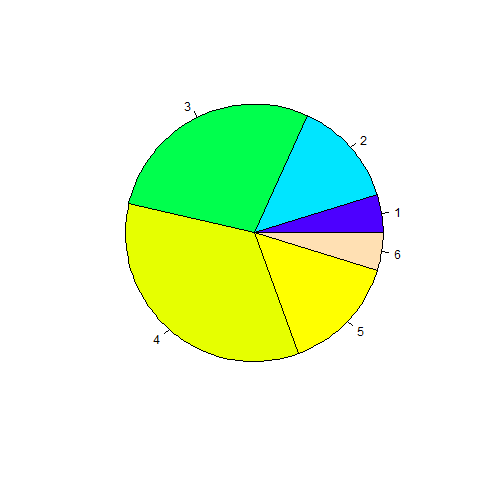
\includegraphics[height=6cm]{../fig/Cap01-DiagramaSectores.png}
% 	\hspace{0.5cm}
	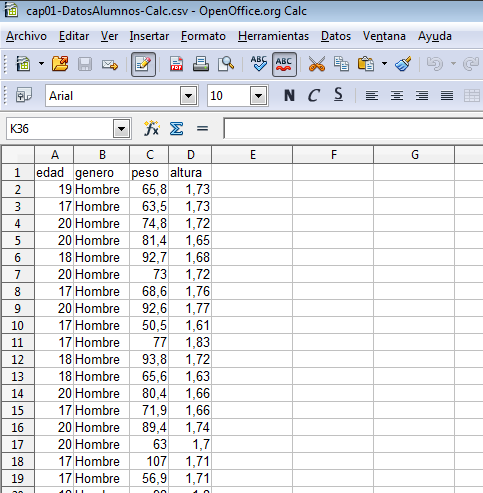
\includegraphics[height=7cm]{../fig/Cap01-DatosAlumnos.png}
	\end{enColor}
	\begin{bn}
% 	\includegraphics[height=6cm]{../fig/Cap01-DiagramaSectores-bn.png}
% 	\hspace{0.5cm}
	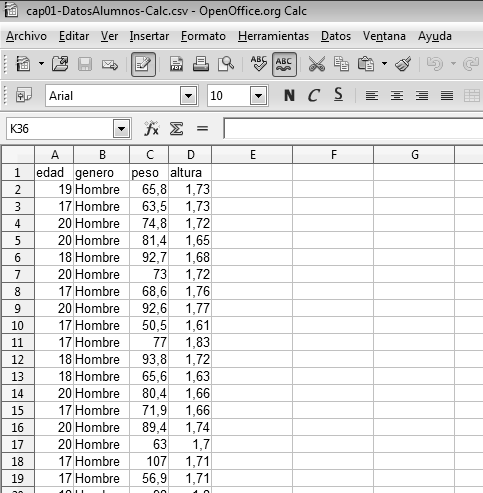
\includegraphics[height=7cm]{../fig/Cap01-DatosAlumnos-bn.png}
	\end{bn}
	\caption{El contenido del fichero {\tt cap01-DatosAlumnos.csv}, en Calc.}
	\label{cap01:fig:DatosAlumnosCalc}
    \end{center}
    \end{figure}


Vamos a utilizar estos datos para ilustrar algunas de las ideas que iremos viendo.

Una observación: si utilizamos $p_1,p_2,\ldots,p_{100}$ para referirnos, por ejemplo, a los datos de peso de esa tabla,
entonces $p_1$ es el dato en la segunda fila, $p_2$ el dato en la tercera, y
$p_{35}$ el dato de la fila $36$. Porque, como veremos, puede ser
cómodo y conveniente conservar los nombres de las variables en la primera fila
de la tabla de datos. Además, en estos casos puede ser una buena idea
introducir una columna adicional con el índice $i$ que corresponde a $p_i$ ($i$
es el número de la observación).

Un mismo valor de la variable puede aparecer repetido varias veces en
la serie de observaciones. En el fichero de alumnos del que estamos
hablando, la variable {\em edad} toma estos cuatro valores distintos:
\[17,\qquad  18,\qquad 19,\qquad 20\]
Pero, naturalmente, cada uno de esos valores aparece repetido unas cuantas veces; no en vano {!`}hay 100 alumnos! Este {\sf número de repeticiones de un
valor} es lo que llamamos la {\sf frecuencia} \index{frecuencia} de ese valor. Por ejemplo, el valor 20 aparece repetido 23 veces, lo que significa
obviamente que hay 23 alumnos de 20 años de edad en esa clase. ¿Cómo hemos sabido esto? Desde luego, no los hemos contado ``a mano''. Una de las
primeras cosas que haremos en los tutoriales del curso es aprender a obtener la frecuencia en un caso como este.


% , {\em Hombre} o {\em Mujer} (es una
% variable cualitativa o factor, con dos niveles). Pero cada uno de esos valores
% aparece repetido bastantes veces. En concreto en la clase hay 57
% alumnos y 35 alumnas.

El número de repeticiones de un valor, del que hemos hablado en el anterior párrafo, se llama {\sf frecuencia absoluta}\index{frecuencia
absoluta}, para distinguirlo de la {\sf frecuencia relativa}\index{frecuencia relativa}, que se obtiene dividiendo la frecuencia absoluta por $n$ (el
total de observaciones). La frecuencia relativa es un {\em tanto por uno}, y se convierte fácilmente en un {\sf porcentaje}\index{porcentaje y
frecuencia relativa}, multiplicándola por 100. Volveremos sobre este tema en el Capítulo \ref{cap:ValoresCentralesDispersion} (ver la página \pageref{cap02:subsubsec:MedianaTablasFrecuenciasRelativasAcumuladas}).
%\fernando{¿Cuándo nos conviene hablar de frecuencias acumuladas? Yo creo que mejor en el segundocapítulo...}


Cuando tratamos con variables cualitativas o discretas, muchas veces, en lugar del valor de cada observación la información que tenemos es la
de las frecuencias de cada uno de los posibles valores distintos de esas variables. Esto es lo que se conoce como una {\sf tabla de
frecuencias}\index{tabla de frecuencias}. Por ejemplo, la Tabla \ref{cap01:tabla:FrecuenciaEdadClase} (pág.\pageref{cap01:tabla:FrecuenciaEdadClase})
es la tabla de frecuencia de la variable edad en este ejemplo

\begin{table}[ht]
\centering
\begin{tabular}{cc}
  \hline
  edad& frecuencia \\
  \hline
  17 &  17 \\
  18 &  37 \\
  19 &  23 \\
  20 &  23 \\
   \hline
\end{tabular}
\caption{Tabla de frecuencia. variable edad en el ejemplo de una clase ficticia.}
\label{cap01:tabla:FrecuenciaEdadClase}
\end{table}
Para distinguirlas de las frecuencia relativas, y de otros tipos de frecuencias que vamos a ver en el Capítulo \ref{cap:ValoresCentralesDispersion}, a veces llamaremos a estas {\sf frecuencias absolutas}\index{frecuencias absolutas}

¿Qué sucede en este ejemplo con la variable peso? ¿Podemos calcular
una tabla de frecuencias? Sí, en principio, podemos. Pero hay demasiados valores
distintos, y la información presentada así no es útil. De hecho, como el peso
{\em es una variable (cuantitativa) continua}, si nos dan los
pesos de los alumnos en kilos, con, por ejemplo, dos cifras decimales, algo como 56.41kg, {\em es muy posible
que no haya dos alumnos con el mismo valor de la variable} peso. Por otra parte,
si los pesos de varios alumnos se diferencian en unos pocos cientos de
gramos, seguramente preferiremos representarlos por un valor común (el mismo
para todos los alumnos de pesos parecidos). En el caso de variables continuas,
lo habitual es {\em dividir el recorrido de posibles valores de esa variable
continua en intervalos}, que también se llaman clases\index{clase (variables continuas agrupadas)}.
Y además se elige a un valor particular, llamado la {\sf marca de clase}\index{marca de clase}, como representante de todos los valores que pertenecen
a ese intervalo. Si el intervalo es $(a,b]$ (es decir, los valores $x$ que cumplen $a<x\leq b$), lo habitual es tomar como marca de clase el punto medio de ese intervalo; es decir, el valor:
\begin{center}
        \fcolorbox{black}{Gris025}{\begin{minipage}{2.5cm}\[\dfrac{a+b}{2}\]\end{minipage}}
\end{center}
Por cierto, tomamos los intervalos de la forma $(a,b]$ para evitar dudas o ambigüedades sobre a qué intervalo pertenecen los extremos.


Una {\sf tabla de frecuencia por intervalos} muestra, para estas variables, cuantos de los valores observados caen dentro de
cada uno de los intervalos. En el ejemplo que estamos utilizando, podemos dividir arbitrariamente los
valores del peso en intervalos de 10 kilos, desde 40 hasta 110, y obtenemos
la tabla de frecuencias (se muestra en disposición horizontal, dividida en dos filas):
\begin{table}[ht]
\centering
\begin{tabular}{lcccc}
  \hline
Peso (kg) entre & (40,50] & (50,60] & (60,70] & (70,80] \\
  \hline
Número de alumnos &   1 &  20 &  21 &  29\\
   \hline\hline
Peso (kg) entre & (80,90] & (90,100] & (100,110] \\
  \hline
Número de alumnos &    20 &   7 &   2 \\
   \hline
\end{tabular}
\caption{Tabla de frecuencia, variable peso agrupada en intervalos.}
\label{cap01:tabla:FrecuenciaPesoClase}
\end{table}




% \begin{center}
%     \begin{tabular}{|c|c|c|}
%     \hline
%     {\bf Intervalo}&{\bf Significado}&{\bf Frecuencia}\\ \hline
%     (75,85]&Peso$<$85&0\\ \hline
%     (85,95]&85$<$Peso$\leq$95&1\\ \hline
%     (95,105]&95$<$Peso$\leq$105&1\\ \hline
%     (105,115]&105$<$Peso$\leq$115&7\\ \hline
%     (115,125]&115$<$Peso$\leq$125&15\\ \hline
%     (125,135]&125$<$Peso$\leq$135&10\\ \hline
%     (135,145]&135$<$Peso$\leq$145&13\\ \hline
%     (145,155]&145$<$Peso$\leq$155&22\\ \hline
%     (155,165]&155$<$Peso$\leq$165&7\\ \hline
%     (165,175]&165$<$Peso$\leq$175&6\\ \hline
%     (175,185]&175$<$Peso$\leq$185&4\\ \hline
%     (185,195]&185$<$Peso$\leq$195&5\\ \hline
%     (195,205]&195$<$Peso$\leq$205&0\\ \hline
%     (205,215]&205$<$Peso$\leq$215&1\\ \hline
%     (215,225]&210$<$Peso&0\\ \hline
%     \end{tabular}
%     \end{center}
%     \calcLogo {Y aquí} está el correspondientes fichero Calc:
% \textattachfile{../fig/Cap01-GonickSmith-p009-frecuenciasPesos.ods}{
% \textcolor{blue}{Cap01-GonickSmith-p009-frecuenciasPesos.ods}}.

Algunos comentarios adicionales sobre esta tabla:
\begin{enumerate}
 \item El proceso para obtener estas tablas de frecuencias por intervalos es algo más complicado. De nuevo nos remitimos a los tutoriales, en este caso al {\sf Tutorial01},
en el que veremos en detalle cómo se hace esto en una hoja de cálculo. Además, este proceso está relacionado con la distinción entre valores
cuantitativas discretas y continuas (ver pág. \pageref{cap01:subsec:VariablesCuantDiscretasContinuas}). Ya dijimos que esa diferencia era una
cuestión sutil, que iría quedando más clara con la experiencia.
  \item Los intervalos, insistimos, se han elegido de manera arbitraria en este ejemplo. Invitamos al lector a pensar cómo cambiaría la
información de la tabla de frecuencias si eligiéramos un número distinto de intervalos, o si, por ejemplo, los intervalos no fueran
todos de la misma longitud.
\end{enumerate}

Cuando los valores de una variable continua se presentan en
forma de tabla de frecuencias por intervalos hablaremos de {\sf datos
agrupados}. En cualquier caso, conviene recordar que una tabla de frecuencias es
una forma de resumir la información, y que al pasar del conjunto de datos
inicial a las tablas de frecuencias de Peso y Género generalmente se pierde
información.



\section{Tablas y representación gráfica de datos.}
\label{cap01:sec:TablasRepresentacionGraficaDatos}

Una vez organizados y resumidos los datos en tablas queremos
extraer la información que contienen. En primera instancia es recomendable
hacer una exploración visual, para lo que resulta extremadamente útil
trasladar el contenido de las tablas a gráficas. Vamos a ver, en este apartado, algunos de los tipos básicos
(y clásicos) de diagramas que se pueden utilizar para visualizar las tablas de frecuencia. Pero no queremos dejar de
decir que el tema de la visualización de datos es muy amplio, que es un campo donde la actividad es ahora mismo febril,
y que a lo largo de los próximos capítulos iremos viendo otros ejemplos de representación gráfica de la información.
%\subsection*{Contenido:}
%
%\begin{enumerate}
% \item Diagramas de líneas, sectores y barras
% \item Histogramas
%\end{enumerate}

\subsection{Diagramas de sectores y barras.}
\label{cap01:subsec:DiagramasSectoresBarras}

Los diagramas de sectores y barras se utilizan cuando queremos mostrar
  frecuencias (o porcentajes, recuentos, etcétera). Se pueden utilizar
  para ilustrar las frecuencias de variables tanto cualitativas como
  cuantitativas. A continuación vamos a describir un ejemplo de cada uno de estos tipos de diagrama, usando en ambos
  casos los datos del fichero \fichero{../datos/Cap01-DiagramaBarrasSectores.csv}{Cap01-DiagramaBarrasSectores.csv}. Este fichero
  contiene 1500 números enteros aleatorios, del 1 al 6.  La tabla de frecuencias es esta:
  \begin{center}
    \begin{tabular}{rrrrrrr}
      \hline
      Valor & 1 & 2 & 3 & 4 & 5 & 6 \\
      \hline
      Frecuencia &  72 & 201 & 423 & 512 & 222 &  70 \\
      \hline
    \end{tabular}
  \end{center}

Los diagramas de \index{diagrama de sectores circulares} {\sf sectores circulares}, como el de la Figura \ref{cap01:fig:DiagramaSectores},
  son útiles para  mostrar proporciones, pero sólo cuando los valores son bastante distintos entre sí. Porque, pese a su popularidad, en  muchas
  ocasiones pueden resultar confusos o poco precisos. Por ejemplo, en esa figura ¿qué frecuencia es mayor, la del grupo 2 o la del grupo 5?
    \begin{figure}[h]
	\centering
	\begin{enColor}
% 	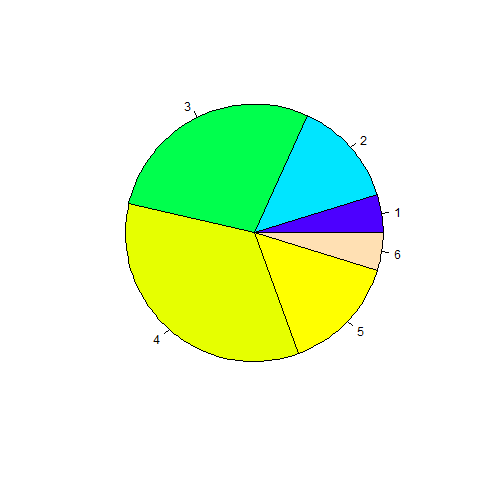
\includegraphics[height=6cm]{../fig/Cap01-DiagramaSectores.png}
% 	\hspace{0.5cm}
	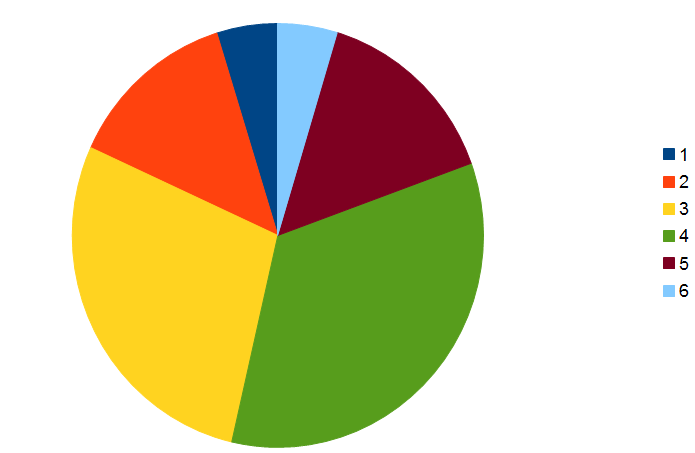
\includegraphics[height=7cm]{../fig/Cap01-DiagramaSectoresconCalc.png}
	\end{enColor}
	\begin{bn}
% 	\includegraphics[height=6cm]{../fig/Cap01-DiagramaSectores-bn.png}
% 	\hspace{0.5cm}
	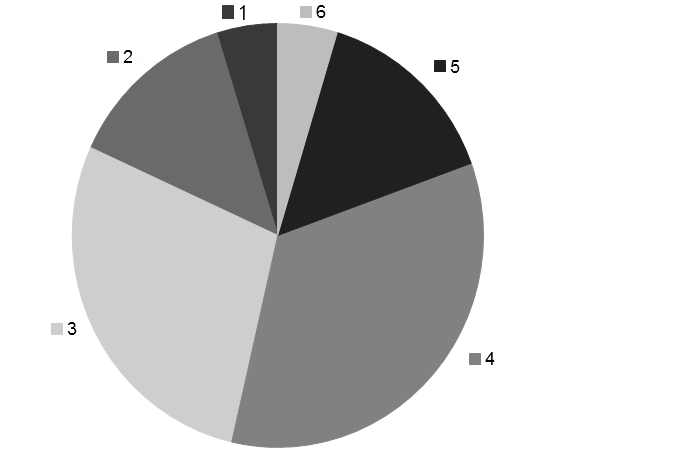
\includegraphics[height=7cm]{../fig/Cap01-DiagramaSectoresconCalc-bn.png}
	\end{bn}
	\caption{Diagrama de sectores circulares, dibujado con Calc.}
	\label{cap01:fig:DiagramaSectores}
    \end{figure}

Los \index{diagrama de barras o columnas} {\sf diagramas de barras o columnas}\index{barras, diagrama de }\index{columnas, diagrama de} tienen,
  en general, más precisión que los de sectores. En la parte (a) de la Figura
  \ref{cap01:fig:DiagramaBarras} se muestra el mismo conjunto de valores que antes vimos en el diagrama de sectores. Y ahora es evidente que, aunque
  son muy parecidas, la frecuencia del valor 2 es menor que la del valor 5. Además, los diagramas de barras se pueden utilizar para  mostrar varios conjuntos de datos simultáneamente, facilitando la comparación entre ellos, como en la parte (b) de la Figura  \ref{cap01:fig:DiagramaBarras}.
  \begin{figure}[phtb]
	\begin{center}
	\begin{enColor}
    (a)\\
	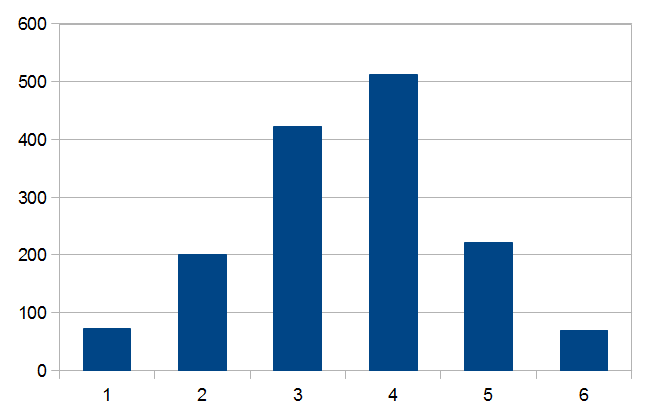
\includegraphics[width=10cm]{../fig/Cap01-DiagramaBarrasconCalc.png}\\[3mm]
    (b)\\
    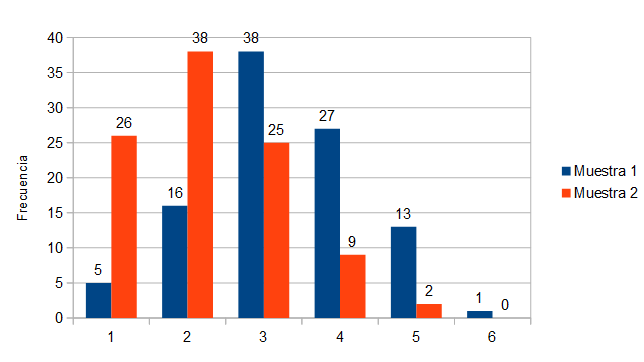
\includegraphics[width=10cm]{../fig/Cap01-DiagramaBarrasDosMuestras.png}\\[3mm]
	\end{enColor}
	\begin{bn}
    (a)\\
	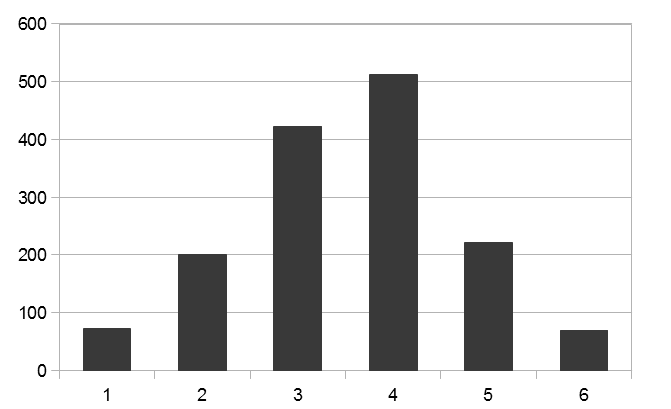
\includegraphics[width=10cm]{../fig/Cap01-DiagramaBarrasconCalc-bn.png}\\[3mm]
    (b)\\
    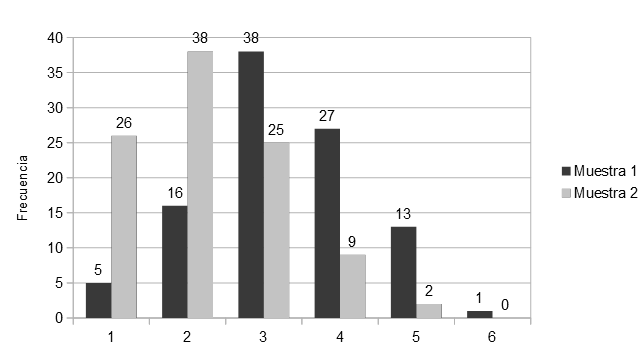
\includegraphics[width=10cm]{../fig/Cap01-DiagramaBarrasDosMuestras-bn.png}\\[3mm]
	\end{bn}
	\caption{Diagrama de barras para (a) un conjunto de datos, (b) dos conjuntos de datos.}
	\label{cap01:fig:DiagramaBarras}
    \end{center}
  \end{figure}

En los tutoriales aprenderemos a dibujar este tipo de gráficos.

%
\subsection{Histogramas.}
\label{cap01:sec:Histogramas}

Un {\sf histograma} \index{histograma}  es un tipo especial de
diagrama   de barras que se utiliza para variables cuantitativas agrupadas en
intervalos (clases) (recuerda la discusión que precedía a la Tabla \ref{cap01:tabla:FrecuenciaPesoClase}, pág.
\pageref{cap01:tabla:FrecuenciaPesoClase}). Puedes ver un ejemplo en la Figura \ref{cap01:fig:Histograma}. Las
dos  propiedades básicas que caracterizan a un histograma son:
    \begin{enumerate}
      \item Las {\em bases de cada una de las barras se corresponden con
      los intervalos} en los que hemos dividido el recorrido de los valores de la
      variable continua.

      \item El {\em área de cada barra es proporcional a la
      frecuencia  correspondiente a ese intervalo.}
    \end{enumerate}

\begin{figure}[h]
\centering
\begin{enColor}
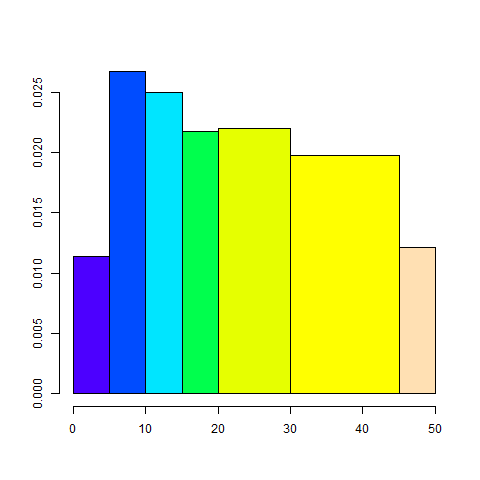
\includegraphics[height=7cm]{../fig/Cap01-Histograma.png}
\end{enColor}
\begin{bn}
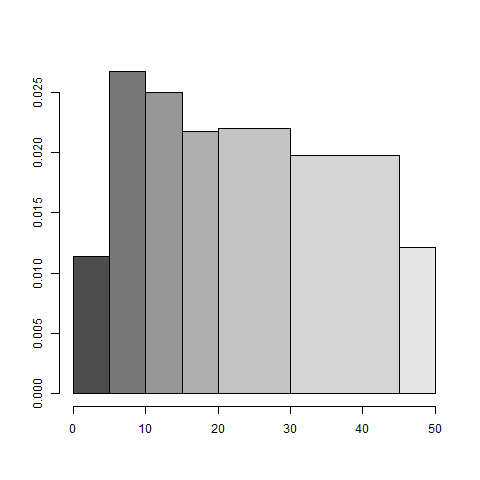
\includegraphics[height=7cm]{../fig/Cap01-Histograma-bn.png}
\end{bn}
\caption{Histograma.}
\label{cap01:fig:Histograma}
\end{figure}

Una consecuencia de estas propiedades es que las columnas de un histograma no tienen porque tener la misma anchura, como se ve en la Figura
\ref{cap01:fig:Histograma}.

Dos observaciones adicionales: en primer lugar, puesto que los
intervalos deben cubrir todo el recorrido de la variable, en un histograma no
hay espacio entre las barras. Y, como práctica recomendable, para que la
visualización sea efectiva, no es conveniente utilizar un histograma con más de
10 o 12 intervalos, ni con menos de cinco o seis.

En el caso de {\sf variables cuantitativas discretas}, normalmente los
intervalos se extienden a valores intermedios (que la variable no puede
alcanzar) para que no quede espacio entre las barras del histograma.

Los pasos para obtener el histograma, en el caso en el que todos los intervalos son de la misma longitud, son estos:
\begin{enumerate}

      \item Si no nos los dan hechos, debemos empezar por determinar los
      intervalos.  Para ello podemos localizar el valor máximo y el mínimo de
      los valores, restarlos y obtenemos el {\em recorrido} de la variable (daremos más detalles en el Capítulo \ref{cap:ValoresCentralesDispersion}).

      \item Dividimos ese recorrido entre el número de intervalos deseados,	
      para obtener la longitud de cada uno de los intervalos. Construimos los
      intervalos y la tabla de frecuencias correspondiente.

      \item Calculamos la altura de cada barra, teniendo en cuenta que
      área=base$\cdot$ altura, y que el área ({!`}no la altura!) es proporcional a
      la frecuencia. Por lo tanto podemos usar:

%      \begin{center}
%        \fbox{\colorbox{Gris025}{
%          \begin{minipage}{8cm}
%	    \[
%	      \mbox{altura}=\dfrac{\mbox{frecuencia}}{\mbox{base}}=\dfrac{\mbox{frecuencia del intervalo}}
%	      {\mbox{anchura del intervalo}}
%	    \]
%          \end{minipage}}
%        }
%     \end{center}
        \begin{center}
                \fcolorbox{black}{Gris025}{\begin{minipage}{8cm}	    \[
        	      \mbox{altura}=\dfrac{\mbox{frecuencia}}{\mbox{base}}=\dfrac{\mbox{frecuencia del intervalo}}
        	      {\mbox{longitud del intervalo}}
        	    \]
        \end{minipage}}
        \end{center}
para calcular la altura de cada una de las barras.
\end{enumerate}
Quizá la mejor manera de entender la propiedad más importante (y más útil) de un histograma sea viendo un {\em falso histograma}, un histograma mal hecho.
\begin{ejemplo}
\label{cap01:ejem:HistogramaMalHecho}
En la Tabla \ref{cap01:tabla:EjemploHistogramaMalHecho} se muestra la tabla de frecuencia de un conjunto de datos, agrupados por intervalos (clases). Observa que la longitud del último intervalo, el intervalo $(8,12]$, es el doble de las longitudes de los restantes intervalos, que son todos de longitud $2$.

\begin{table}[ht]
\centering
\begin{tabular}{|l|rrrrr|}
  \hline
Clase & [0,2] & (2,4] & (4,6] & (6,8] & (8,12] \\
  \hline
Frecuencia & 1320 & 3231 & 1282 & 900 & 1105 \\
   \hline
\end{tabular}
\caption{Datos para el Ejemplo \ref{cap01:ejem:HistogramaMalHecho}}
\label{cap01:tabla:EjemploHistogramaMalHecho}
\end{table}

En la parte (a) de la Figura \ref{cap01:fig:Histograma} se muestra un falso histograma, en el que la altura de las columnas se corresponde con esas frecuencias. Para un observador que no disponga de la Tabla \ref{cap01:tabla:EjemploHistogramaMalHecho} (e incluso si dispone de ella, en muchos casos), la sensación que transmite ese gráfico es que el número de casos que corresponden al intervalo $(8,12]$ es mucho mayor que los del intervalo $(6,8]$. Resulta poco claro, en esta representación gráfica, el hecho relevante de que esa frecuencia mayor se corresponde con un intervalo el doble de ancho. El sistema perceptivo humano tiende a dar más importancia a las figuras con mayor área, especialmente si sus alturas son parecidas.

\begin{figure}[hbpt]
\centering
\begin{enColor}
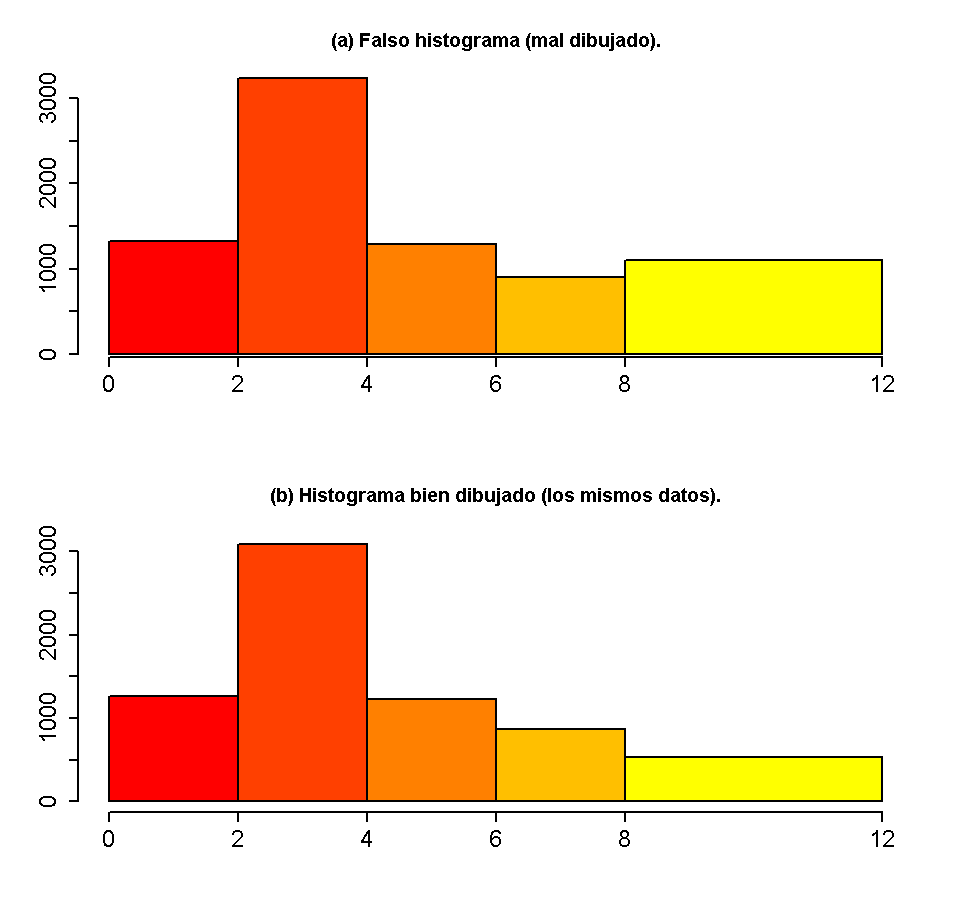
\includegraphics[width=12cm]{../fig/Cap01-HistogramaMalHecho.png}
\end{enColor}
\begin{bn}
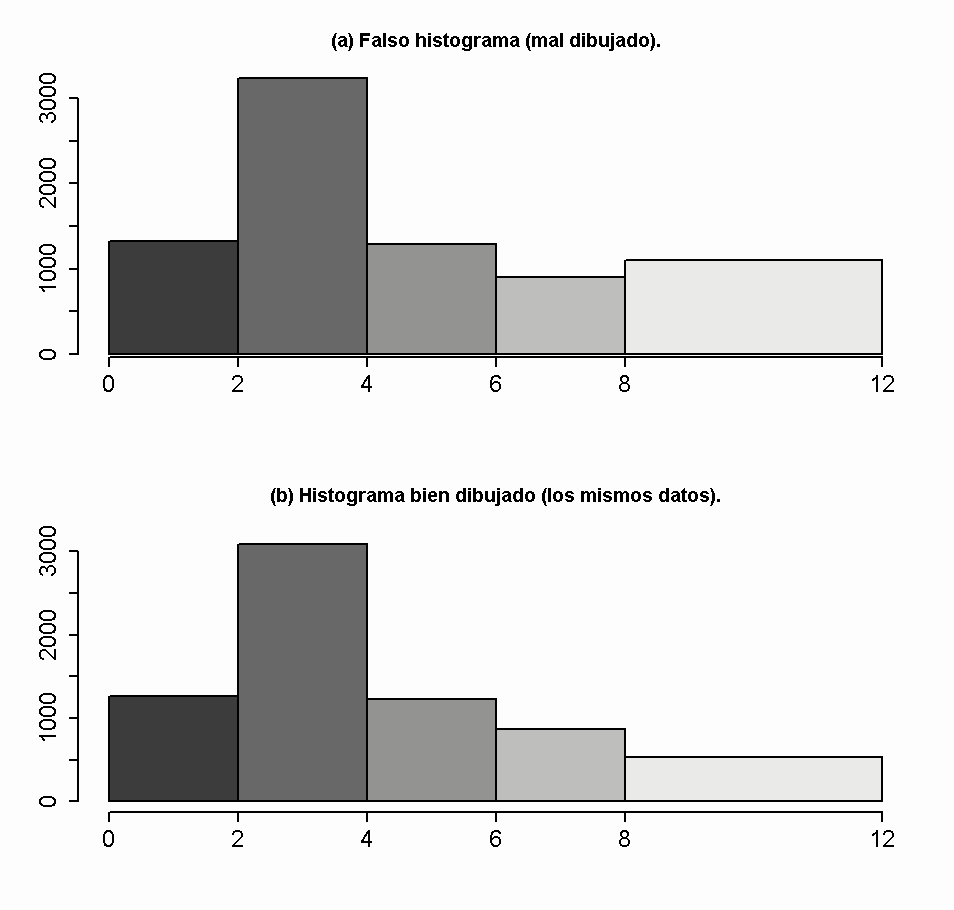
\includegraphics[width=12cm]{../fig/Cap01-HistogramaMalHecho-bn.png}
\end{bn}
\caption{Representación de los datos del Ejemplo \ref{cap01:ejem:HistogramaMalHecho}, con un (a) falso histograma (con {\em la altura} proporcional a la frecuencia), y (b) el histograma correcto para esos mismos datos (con {\em el área} proporcional a la frecuencia).}
\label{cap01:fig:Histograma}
\end{figure}
\end{ejemplo}

En la parte (b) de esa Figura, por otra parte, aparece el histograma correctamente dibujado. Como puede apreciarse, el hecho de hacer que sea el área de la columna lo que se corresponda con la frecuencia, ayuda a captar visualmente la importancia relativa del intervalo $(8,12]$. De esta manera queda de manifiesto que la anchura de ese intervalo es distinta de las otras, sin sobrevalorar la frecuencia que le corresponde.
\qed

%    \item Pronto aprenderemos a obtener muchos de los resultados de este
%capítulo usando R. Como aperitivo, aquí tenemos un
%\textattachfile{Sesion001.R}{\textcolor{blue}{fichero}} de instrucciones para el
%ejemplo que hemos usado hoy.


%\Pendiente{TODO NUEVO}
\section{Precisión y exactitud. Cifras significativas.}
\label{cap01:sec:PrecisionExactitudCifrasSignificativas}

Vamos a aprovechar la sección final de este capítulo para introducir algunas herramientas de lenguaje, y procedimientos de trabajo con datos
numéricos que usaremos a lo largo de todo el libro. Hemos repetido varias veces en este capítulo que la diferencia entre variables cuantitativas discretas y continuas es bastante sutil. En particular, en el caso de datos agrupados en clases (ver el apartado
\ref{cap01:subsec:NotacionVariablesTablasFrecuenciaDatosAgrupados} y especialmente la discusión de la pág. \pageref{cap01:tabla:FrecuenciaPesoClase}),
surge la pregunta de cómo definir el límite entre dos clases. Aunque en los tutoriales veremos cómo hacer esto en la práctica, podemos preparar el terreno. Esta cuestión, a su vez, está estrechamente ligada a la cuestión de las unidades de medida
que se utilizan, y de la precisión con la que obtenemos esas medidas. Volviendo al ejemplo de los alumnos de una clase, es muy extraño pensar que
alguien nos va a decir que uno de esos alumnos pesa 65.2365789 kilogramos. ¿De verdad nos creemos que tiene sentido expresar así el peso de una
persona, cuando la pérdida de un sólo cabello\footnote{Una persona tiene aproximadamente cien mil pelos en la cabeza, cada uno de unos miligramos de peso.} cambiaría esa cifra en una
escala mucho mayor que la supuesta ``precisión'' de la medida? Naturalmente que no. Por esa razón, al hablar del peso de una persona lo más
{\em práctico} es trabajar en kilos, a lo sumo en cientos o decenas de gramos. Al hacer esto, sucede algo interesante: si usamos los kilos como
unidad de medida, sin preocuparnos de diferencias más finas, diremos que un alumno pesa 57 kilos y otro 58 kilos, pero no diremos nunca que pesa 55'5
o 55'32 kilos. Es decir, que al trabajar de esa manera, estaremos usando el peso {\em como si fuera una variable discreta}, que cambia a saltos, de
kilo en kilo. El lector estará pensando {!`}pero el peso \underline{ES} continuo! Y lo que queremos es invitarle a descubrir que el peso no es ni
continuo ni discreto. En distintos problemas usamos distintos modelos, y matemáticas distintas, para trabajar con las medidas de peso. Y la decisión
sobre cuál es el modelo más adecuado depende muchas veces de la precisión y exactitud con las que deseamos trabajar.

Aprovechemos la ocasión para establecer una distinción entre las nociones de precisión y exactitud. Aunque a menudo se usan indistintamente en el
lenguaje cotidiano\footnote{El Diccionario de la Real Academia Española (ver enlace [\,\ref{enlace0000-2}\,]\label{enlace0000a-2}) nos
parece especialmente poco atinado en estas dos entradas...}, estas dos nociones tienen significados técnicos distintos. No queremos entrar en una
discusión demasiado técnica, así que vamos a recurrir, para ilustrar la diferencia entre ambas nociones a la imagen, que se usa a menudo de una diana
a la que estamos tratando de acertar. La idea se ilustra en la Figura \ref{cap01:fig:PrecisionExactitud} (pág.
\pageref{cap01:fig:PrecisionExactitud}). Como puede verse, la idea de precisión se
relaciona con la distancia al objetivo (con el tamaño del error que se comete, visto de otra manera.)  En cambio, la idea de exactitud tiene que ver
con la posición de nuestros disparos, y con el hecho de que esos disparos estén {\em centrados} en el blanco.
    \begin{figure}[h]
	\centering
	\begin{enColor}
% 	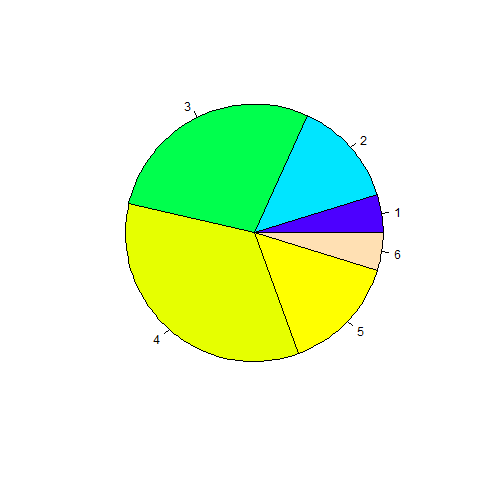
\includegraphics[height=6cm]{../fig/Cap01-DiagramaSectores.png}
% 	\hspace{0.5cm}
	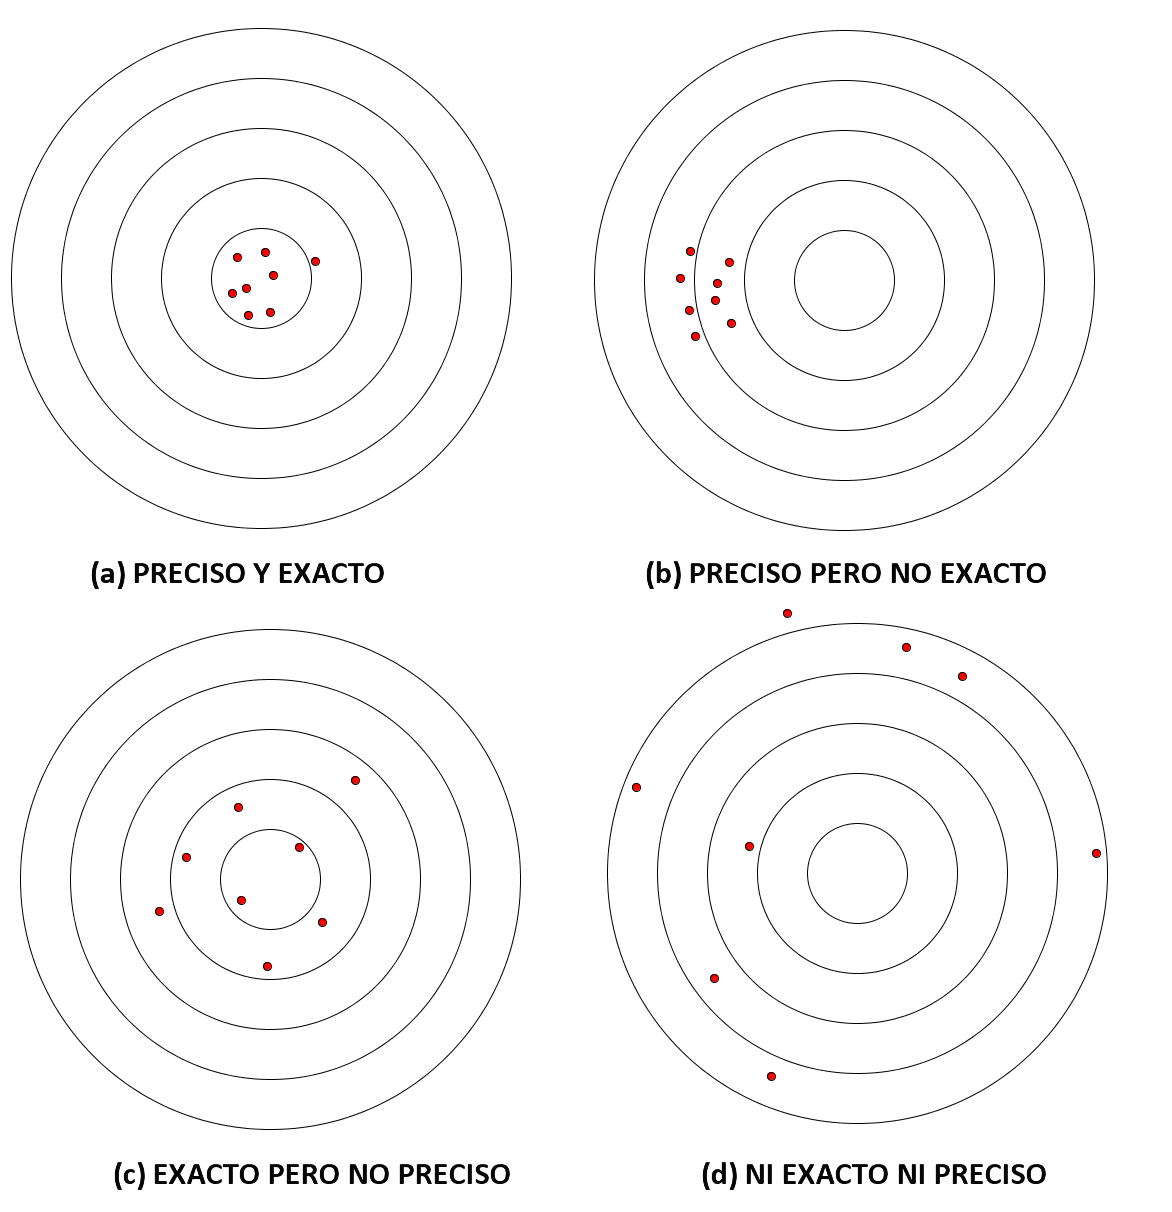
\includegraphics[width=10cm]{../fig/Cap01-PrecisionExactitud-2.png}
	\end{enColor}
	\begin{bn}
% 	\includegraphics[height=6cm]{../fig/Cap01-DiagramaSectores-bn.png}
% 	\hspace{0.5cm}
	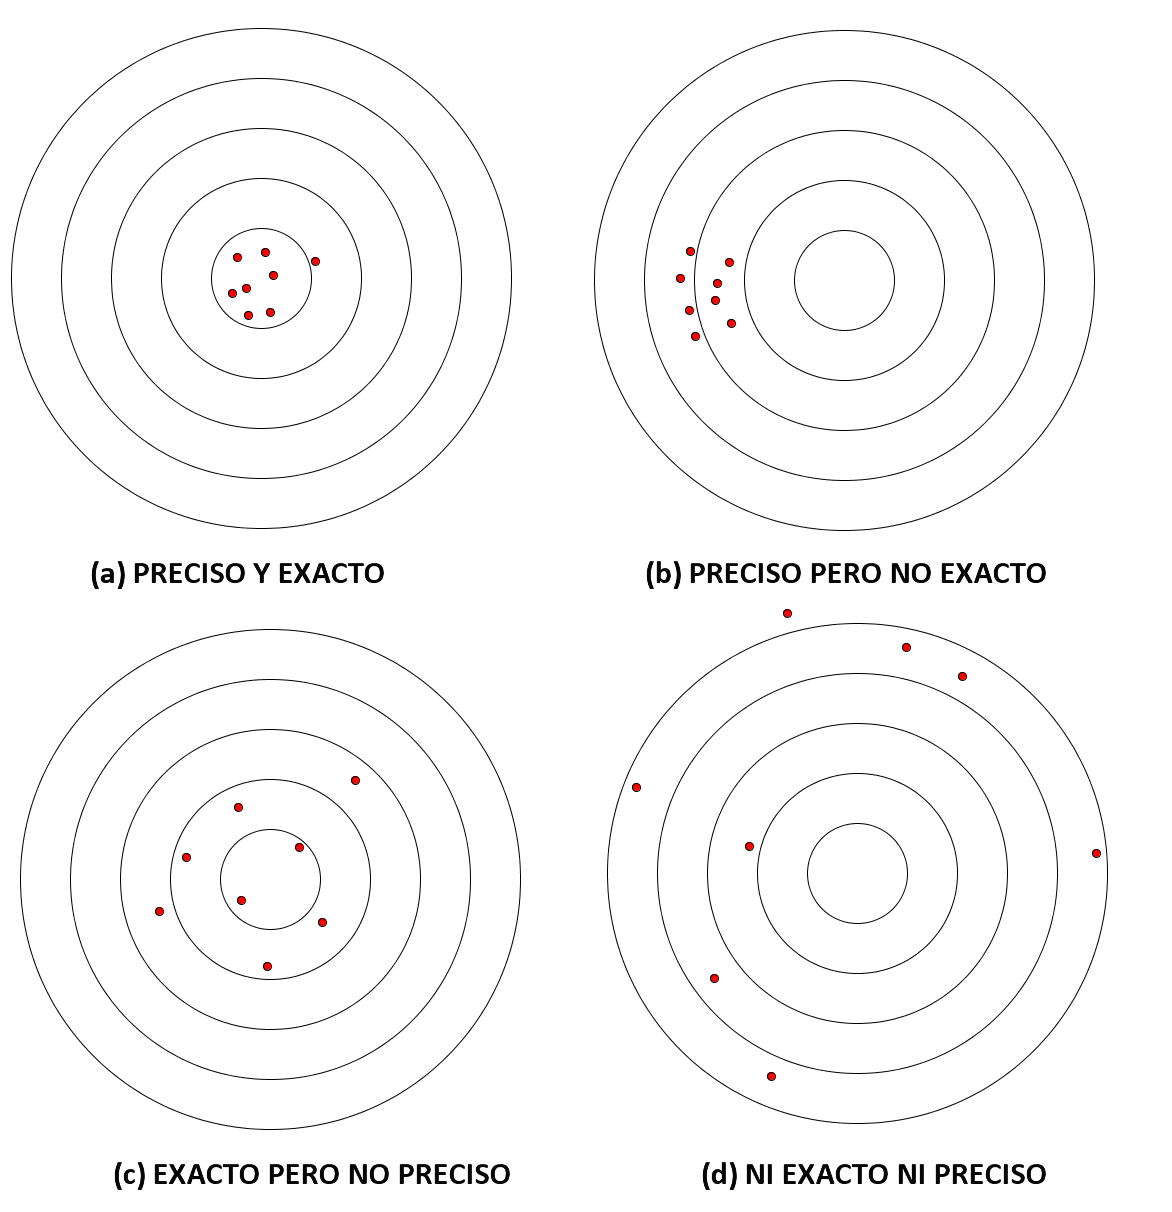
\includegraphics[width=10cm]{../fig/Cap01-PrecisionExactitud-2.png}
	\end{bn}
	\caption{Precisión y exactitud.}
	\label{cap01:fig:PrecisionExactitud}
    \end{figure}

A lo largo del curso, y muy especialmente en el próximo capítulo, vamos a tener sobradas ocasiones de volver sobre estas dos ideas. Pero ya que
vamos a trabajar muy a menudo con valores numéricos, vamos a hablar del concepto de {\sf cifras significativas}\index{cifras significativas}, que está
muy relacionado con la idea de precisión de las medidas.

Todos los números que proceden de mediciones tienen una precisión limitada, ligada a menudo al propio aparato o proceso de medición. Por ejemplo, y
para que no suene muy abstracto, si medimos una longitud con una regla típica, la precisión de la medida sólo llega al milímetro, porque esas son las
divisiones de la escala en nuestra regla. De la misma forma un termómetro doméstico no suele afinar más allá de las décimas de grado, la balanza de
cocina distingue normalmente, a lo sumo, gramos, etcétera.

Por esa razón, si hemos medido con la regla una longitud de 5cm, o sea 50mm, y lo hemos hecho teniendo cuidado de precisar hasta el milímetro, sabemos
que en realidad sólo hemos sido capaces de asegurar que el valor de la longitud está entre
\[50-1=49,\qquad\mbox{ y }\qquad 50+1=51\mbox{ mm.}\]
Hasta aquí las cosas son relativamente fáciles. El problema viene, habitualmente, cuando se hacen operaciones con los resultados de las medidas. Por
ejemplo, si dividimos esa longitud en tres trozos iguales, ¿cuánto medirán esos tres trozos? Si tecleamos en una calculadora $50/3$ podemos terminar
respondiendo algo como que esos trozos miden:
\[16.66666667\mbox{ mm.}\]
Así, mediante el procedimiento mágico de aporrear las teclas de una calculadora, resulta que una medida que sólo conocíamos con una precisión de un
milímetro se ha convertido en un resultado preciso casi hasta la escala atómica. Evidentemente esta no es la forma correcta de trabajar. Es necesario
algún proceso de {\sf redondeo}\index{redondeo, cifras significativas} para obtener un resultado preciso.

Uno de los objetivos secundarios de este curso es proporcionar al lector una formación básica en el manejo de los números como instrumentos de
comunicación científica. Vamos a empezar, en este apartado, por familiarizarnos con la noción de cifras significativas, y poco a poco, en sucesivas
visitas a este tema, iremos aprendiendo cómo se manejan correctamente situaciones como la que hemos descrito, en la que hacemos operaciones con
números aproximados. Trataremos, también en esto, de darle un enfoque siempre eminentemente práctico a lo que hagamos.

Así que, en lugar de empezar tratando de definir qué son las cifras significativas, comencemos con algunos ejemplos, para ilustrar la forma de proceder.

\begin{Ejemplo}
Supongamos que nos dan el número
\[1.623698\]
y nos piden que lo redondeemos a cuatro cifras significativas. Se trata, por tanto, de aprender a redondear un número dado, en notación decimal, a una cierta cantidad de cifras significativas (cuatro, en este ejemplo). El procedimiento es
este:
\begin{enumerate}
  \item empezando desde la primera cifra del número (la situada más a la izquierda), buscamos la primera cifra que no sea un cero. En el ejemplo esa cifra es $1$, la primera del número por la izquierda.
  \[
    \begin{array}{cccccccc}
      \mathbf{1}&.&6&2&3&6&9&8\\
      \mathbf{\uparrow}\\
    \end{array}
  \]
  Para este paso no importa la posición del punto decimal. La única duda que se puede plantear es si hay ceros a la izquierda, y ese caso lo veremos enseguida, más abajo.
  \item Como queremos cuatro cifras significativas, empezamos a contar desde esa primera cifra (inclusive) hacia la derecha, hasta llegar a  cuatro cifras.
  \[
    \begin{array}{cccccccc}
      1&.&6&2&3&6&9&8\\
      \mathbf{\uparrow}&&\mathbf{\uparrow}&\mathbf{\uparrow}&\mathbf{\uparrow}\\
      1^o&&2^o&3^o&4^o
    \end{array}
  \]
  \item Ahora miramos la siguiente cifra, en este caso la quinta (que es un seis). Y aplicamos esta regla de decisión: si la quinta cifra es mayor o igual que 5, sumamos 1 a la cuarta cifra, con acarreo si es necesario (veremos esto en el siguiente ejemplo). En el ejemplo,
  \[
    \begin{array}{cccccccc}
      1&.&6&2&3&\mathbf{6}&9&8\\
      &&&&&\mathbf{\uparrow}\\
      &&&&&5^o
    \end{array}
  \]
  Como la quinta cifra es 6, y por lo tanto mayor o igual a 5,  sumamos 1 a la última cifra de 1.623 (las cuatro primeras cifras no nulas del número original) y obtenemos:
  \[1.62\mathbf{4}.\]
  Este es el valor de $1.623698$ redondeado a cuatro cifras significativas.
  \end{enumerate}

  Veamos ahora un ejemplo más complicado, en el que entran en juego reglas adicionales de redondeo. De nuevo nos dan un número, en este caso
  \[0.00337995246\]
  y vamos a redondearlo, ahora a cinco cifras significativas. Aplicamos el mismo esquema:
  \begin{enumerate}
  \item Empezando desde la primera cifra del número (la situada más a la izquierda), buscamos la primera cifra que no sea un cero. En el ejemplo esa cifra es $3$, en realidad la cuarta cifra del número por la izquierda (la tercera después del punto decimal).
  \[
    \begin{array}{cccccccccccccc}
      0&.&0&0&\mathbf{3}&3&7&9&9&5&2&4&6\\
      &&&&\mathbf{\uparrow}\\
    \end{array}
  \]
  Los ceros a la izquierda no se tienen en cuenta para el total de cifras significativas.
  \item Como queremos cinco cifras significativas, empezamos a contar desde el 3 que hemos localizado en el paso anterior, y  hacia la derecha, hasta llegar a  cinco cifras.
  \[
    \begin{array}{cccccccccccccc}
      0&.&0&0&\mathbf{3}&\mathbf{3}&\mathbf{7}&\mathbf{9}&\mathbf{9}&5&2&4&6\\
      &&&&\mathbf{\uparrow}&\mathbf{\uparrow}&\mathbf{\uparrow}&\mathbf{\uparrow}&\mathbf{\uparrow}\\
      &&&&1^o&2^o&3^o&4^o&5^o
    \end{array}
  \]
  \item Miramos la siguiente cifra, que en este caso es un cinco.
  \[
    \begin{array}{cccccccccccccc}
      0&.&0&0&{3}&{3}&{7}&{9}&{9}&\mathbf{5}&2&4&6\\
      &&&&&&&&&\mathbf{\uparrow}\\
    \end{array}
  \]
  Como esa cifra es mayor o igual a 5,  sumamos 1 a la última cifra de $0.0033799$ (la parte precedente del número original) y obtenemos:
  \[0.0033800.\]
  Fíjate en que hemos hecho la suma con acarreo (dos acarreos, porque había dos nueves al final). Y que, al hacer esto, conservamos los ceros que aparecen a la derecha. Es importante hacer esto, porque esos ceros sí que son cifras significativas (a diferencia de los ceros de la izquierda, que no cuentan).
  Así que el número, redondeado a cinco cifras significativas es $0.0033800$.

  Un último ejemplo. Hasta ahora, en los dos ejemplos que hemos visto, el proceso de redondeo ocurría a la derecha del punto decimal. Pero si nos
  piden que redondeemos el número $324755$ a tres cifras significativas, acabaremos con el número $325000$. Los ceros a la derecha son, en este caso,
  imprescindibles. Este último ejemplo pretende ayudar a clarificar un hecho básico: el proceso de redondeo a cifras significativas, {\em nunca} afecta a la
  posición de la coma decimal en el número.  \flushright$\Box$
\end{enumerate}
\end{Ejemplo}
Naturalmente, esta receta no agota la discusión, ni mucho menos. Para empezar, no hemos dicho nada sobre la forma de {\em operar} con números aproximados. Si tengo dos números con cuatro cifras significativas y los multiplico, ¿cuántas cifras significativas tiene el producto? ¿Y qué sucede si calculo la raíz cuadrada de un número con tres cifras significativas?  Veamos un ejemplo sencillo, para que el lector comprenda de que se trata:
\begin{ejemplo}
Tenemos los dos números
\[\begin{cases}
a= 10000\\
b= 2.1
\end{cases}\]
y suponemos que los dos tienen dos cifras significativas, que se han redondeado usando el procedimiento que hemos descrito. En el caso de $a$, y con las reglas de redondeo que hemos dado esto significa que sólo podemos asegurar que $a$ cumple:
\[10000-499< a < 10000+499 \]
Y en particular, al calcular la suma $a+b$ no tiene ningún sentido decir que es
\[a+b=10002.1\]
porque esto parece estar diciendo que conocemos $a+b$ con mucha más precisión de la que conocemos el propio número $a$. Lo razonable en este caso es decir que
\[a+b\approx a\]
donde el símbolo $\approx$ se lee {\em aproximadamente}, e indica el efecto del redondeo. Al sumar, el número $b$ ``ha desaparecido''. En cambio, si multiplicamos, está claro que debe suceder algo como
\[a\cdot b\approx 21000.\]
Y aún pueden suceder cosas peores. Imagínate que tenemos los números
\[\begin{cases}
c= 43.12\\
d= 43.11
\end{cases}\]
ambos con cuatro cifras significativas, y los restamos. ¿Cuántas cifras significativas tiene el resultado? Como puede verse, es necesario algo más de reflexión para operar acertadamente con números aproximados.
\qed
\end{ejemplo}
Este tipo de preguntas tienen su respuesta detallada en una parte de las Matemáticas llamada {\sf Análisis (o Cálculo) Numérico}\index{análisis numérico}\index{numérico, análisis o cálculo}. En general, cada operación con números aproximados supone una pérdida de precisión. Pero aquí no queremos extendernos, y vamos a dejar sin respuesta esas preguntas. Por el momento, nos basta con que el lector comprenda este procedimiento de redondeo a un número de cifras significativas dado. En la práctica, dado que usaremos el ordenador para la mayor parte de las operaciones, vamos a asumir que, en casi todos los casos, la precisión con la que trabaja la máquina es suficiente para compensar la pérdida de precisión asociada a las operaciones que hacemos. A la larga, ese punto de vista se revela como una ingenuidad, pero de momento no necesitamos más.



\chapter{Valores centrales y dispersión.}
\label{cap:ValoresCentralesDispersion}
% !Mode:: "Tex:UTF-8"


Ahora que ya sabemos resumir la información de los datos en tablas y
presentarlos gráficamente, vamos a dar un paso más. Vamos a sintetizar esa
información en un número, que llamaremos ``valor central''. Una de las ideas centrales de este capítulo es que ese valor central tiene que ser un buen representante del conjunto de datos que estamos usando. También veremos que, como no podía ser de otra manera, la elección del representante adecuado depende de la tarea para la que lo vayamos a utilizar. \\
Pero además, una vez elegido un representante de un conjunto de datos,
querremos saber cómo de representativo es ese valor central, respecto del
conjunto de datos que describe. Eso nos llevará a hablar de la idea de
dispersión. La dispersión es, precisamente, una medida de la calidad del valor
central, como representante de un conjunto de datos. Es una noción directamente
emparentada con la idea de precisión, de la que hablamos en el capítulo
anterior (ver Figura \ref{cap01:fig:PrecisionExactitud} en la pág.
\pageref{cap01:fig:PrecisionExactitud}).

\section{La media aritmética.}
\label{cap02:sec:MediaAritmetica}

Vamos a aprovechar este concepto, que suponemos ya conocido del lector, para
introducir parte de la notación abstracta, típica de las Matemáticas, que
utilizaremos a lo largo del curso. Esta sección puede servir de ``chequeo
preliminar'' para el lector. Si tienes muchas dificultades con la notación en
este punto inicial del curso, es probable que necesites reforzar tus
habilidades matemáticas para poder seguir adelante. En los tutoriales 1 y 2 aprenderemos, entre otras cosas, a realizar estos cálculos en el ordenador.

\subsection{Definición de la media aritmética.}
\label{cap02:subsec:DefincionMediaAritmetica}

La idea de media aritmética apenas necesita presentación. Dados $n$ valores de una {\sf variable
cuantitativa}, sean $x_1,x_2,\ldots,x_n$, su {\sf media aritmética} \index{media aritmética} (en
inglés, {\em arithmetic mean} o {\em average}) \index{mean}\index{arithmetic mean}\index{average}
es:
    \begin{center}
        \fcolorbox{black}{Gris025}{\begin{minipage}{8cm}
        \centering{\bf Media aritmética: }
            \begin{equation}
            \label{cap02:ecu:MediaAritmetica}
            \bar x=\dfrac{x_1+\cdots+x_n}{n}=\dfrac{\displaystyle\sum_{i=1}^nx_i}{n}.
            \end{equation}
    \end{minipage}}
    \end{center}
Algunos comentarios sobre la notación. El símbolo $\bar x$ refleja la notación establecida en Estadística: la media de un vector de datos se representa con una barra sobre el nombre de ese vector. Y el símbolo $\displaystyle\sum_{i=1}^n x_i$, que suponemos que el lector ya conoce, es un {\sf sumatorio}, \index{sumatorio} y representa en forma abreviada, la frase ``suma todos estos valores $x_i$ donde $i$ es un número que va desde 1 hasta $n$''.

Insistimos en esto: la {\bf media aritmética sólo tiene sentido para variables
cuantitativas} (discretas o continuas). Aunque una variable cualitativa se
represente numéricamente, la media aritmética de esos números seguramente sea
una cantidad sin ningún significado estadístico.

La media aritmética es ``la media'' por excelencia. Pero hay otros conceptos de
media que juegan un papel importante en algunos temas: la media geométrica, la
media armónica, etc. Pero no las vamos a necesitar en este curso, así que no
entraremos en más detalles.

\begin{ejemplo}
\label{cap02:ejem:MediaAritmetica}
Dado el conjunto de valores (son $n=12$ valores)
\[9,\, 6,\, 19,\, 10,\, 17,\, 3,\, 28,\, 19,\, 3,\, 5,\, 19,\, 2,\]
su media aritmética es:
{\scriptsize
\[\bar x=\dfrac{9 + 6 + 19 + 10 + 17 + 3 + 28 + 19 + 3 + 5 + 19 + 2}{12}=\]
}
\[=\dfrac{140}{12}\approx 11.67,\]
(cuatro cifras significativas). Proponemos al lector como ejercicio que piense si el número $\bar x=11.67$ se puede considerar, en este caso, un buen representante de este conjunto de datos.
\qed
\end{ejemplo}

El siguiente ejemplo sirve para presentar una característica de la media aritmética que debemos tener siempre presente:
\begin{ejemplo}
\label{cap02:ejem:MediaAritmetica02}
Ahora consideramos el mismo conjunto de valores, al que añadimos el número $150$ (en la última posición, aunque su posición es irrelevante para lo que sigue):
\[9,\, 6,\, 19,\, 10,\, 17,\, 3,\, 28,\, 19,\, 3,\, 5,\, 19,\, 2,\, 150\]
La media aritmética ahora es:
{\scriptsize
\[\bar x=\dfrac{9 + 6 + 19 + 10 + 17 + 3 + 28 + 19 + 3 + 5 + 19 + 2 + 150}{13}=\]
}
\[=\dfrac{290}{13}\approx 22.31,\]
(con cuatro cifras significativas). ¿Sigue siendo posible, en este caso, considerar a la media aritmética $\bar x=22.31$ como un buen representante de los datos? Por ejemplo, si elegimos al azar uno cualquiera de esos números, ¿es de esperar que se parezca a la media?
\qed
\end{ejemplo}
Volveremos sobre la pregunta que plantean estos ejemplos en la Sección \ref{cap02:sec:MedianaCuartilesPercentilesModa} (pág. \pageref{cap02:sec:MedianaCuartilesPercentilesModa}). Pero antes vamos a pensar un poco más sobre la forma de calcular la media aritmética, si los datos vienen descritos mediante una tabla de frecuencias.


\subsection{La media aritmética a partir de una tabla de frecuencias.}
\label{cap02:subsec:MediaAritmeticaAPartirTablaFrecuencias}


    Supongamos que tenemos una tabla de frecuencias de unos valores, correspondientes a una variable cuantitativa. Es decir, una tabla como esta :
   \begin{center}
        \begin{tabular}{|c|c|}
        \hline
        \rule{0cm}{4mm}{\bf Valor}&{\bf Frecuencia}\\ \hline
        \rule{0cm}{4mm}$x_1$&$f_1$\\[2mm] \hline
        \rule{0cm}{4mm}$x_2$&$f_2$\\[2mm] \hline
        $\vdots$&$\vdots$\\[2mm] \hline
        \rule{0cm}{4mm}$x_k$&$f_k$\\[2mm] \hline
        \end{tabular}
        \end{center}
   y  queremos calcular la media aritmética a partir de esta tabla.

   Aquí los valores {\em distintos} de la variable\footnote{Acuérdate de que tenemos $n$ observaciones de la variable, pero puede haber valores repetidos. Aquí estamos usando el número de valores distintos, sin repeticiones, y ese número es $k$.} son $x_1,\ldots,x_k$ y sus frecuencias absolutas respectivas son $f_1,f_2,\ldots,f_k$. Está claro entonces que:
        \[f_1+f_2+\cdots+f_k=(\mbox{núm. de observ. de }x_1)+\cdots+(\mbox{núm. de observ. del valor }x_k)= \]
        \[=(\mbox{suma del número de observaciones de todos los valores distintos})=n\]
        Recordemos que para calcular la media tenemos que sumar el valor de todas (las $n$ observaciones). Y como el valor $x_i$ se ha observado $f_i$ veces, su contribución a la suma es
        \[x_i\cdot f_i=x_i+x_i+\cdots+x_i\quad (\mbox{sumamos $f_i$ veces})\]
        Teniendo en cuenta la contribución de cada uno de los $k$ valores distintos, vemos que
        para calcular la media debemos hacer:
%       \begin{center}
%        \fbox{\colorbox{Gris025}{
%            \begin{minipage}{8cm}
%            {\[
%        \bar x=\dfrac{x_1\cdot f_1+x_2\cdot f_2+\cdots+x_k\cdot f_k}{f_1+f_2+\cdots+f_k}=
%        \dfrac{\displaystyle\sum_{i=1}^k x_i\cdot f_i}{\displaystyle\sum_{i=1}^k f_i}\]}
%           \end{minipage}}
%        }
%        \end{center}
        \begin{center}
                \fcolorbox{black}{Gris025}{\begin{minipage}{8cm}
                	    \[\bar x=\dfrac{x_1\cdot f_1+x_2\cdot f_2+\cdots+x_k\cdot f_k}{f_1+f_2+\cdots+f_k}=
                        \dfrac{\displaystyle\sum_{i=1}^k x_i\cdot f_i}{\displaystyle\sum_{i=1}^k f_i}.\]
        \end{minipage}}
        \end{center}


        \begin{Ejemplo}
        En una instalación deportiva el precio de la entrada para adultos es de \EUR{10} y de \EUR{4} para menores. Hoy han visitado esa instalación $230$ adultos y $45$ menores. ¿Cuál es el ingreso medio por visitante que recibe esa instalación?\\
        Tenemos dos posibles valores de la variable $x=${\em ``precio de la entrada''}, que son $x_1=10$ y $x_2=4$. Además sabemos las frecuencias correspondientes: $f_1=230$ y $f_2=45$. Por lo tanto:
        \[\bar x=\dfrac{x_1\cdot f_1+x_2\cdot f_2}{f_1+f_2}=\dfrac{10\cdot 230+4\cdot 45}{230+45}=9.02\]
        El ingreso medio es de \EUR{9.02} por visitante.\qed
        \end{Ejemplo}

    \subsection{Media aritmética con datos agrupados.}
    \label{cap02:subsec:MediaAritmeticaConDatosAgrupados}

    Si lo que queremos es calcular la media aritmética a partir de la tabla de frecuencias agrupadas por intervalos de una variable cuantitativa (ver el final de la Sección \ref{cap01:subsec:NotacionVariablesTablasFrecuenciaDatosAgrupados}), las cosas son (sólo un poco)  más complicadas. En este caso vamos a tener una tabla de frecuencias por intervalos (recuerda que los intervalos a veces se llaman también {\sf clases}) como esta:
        \begin{center}
        \begin{tabular}{|c|c|}
        \hline
        \rule{0cm}{4mm}{\bf Intervalo}&{\bf Frecuencia}\\ \hline
        \rule{0cm}{4mm}$[a_1,b_1)$&$f_1$\\[2mm] \hline
        \rule{0cm}{4mm}$[a_2,b_2)$&$f_2$\\[2mm] \hline
        $\vdots$&$\vdots$\\[2mm] \hline
        \rule{0cm}{4mm}$[a_k,b_k)$&$f_k$\\[2mm] \hline
        \end{tabular}
        \end{center}
        Comparando esta tabla con el caso anterior está claro que lo que nos falta son los valores $x_1,\ldots,x_k$ y, en su lugar, tenemos los intervalos $[a_1,b_1),\ldots,[a_k,b_k)$. Lo que hacemos en estos casos es {\em fabricar} unos valores $x_i$ a partir de los intervalos. Se toma como valor $x_i$ el punto medio del intervalo $[a_i,b_i)$; es decir:
%        \begin{center}
%        \fbox{\colorbox{Gris025}{
%            \begin{minipage}{6cm}
%            {
%        \[x_i=\dfrac{a_i+b_i}{2},\quad \text{ para } i=1,\ldots,n.\]}
%           \end{minipage}}
%        }
%        \end{center}
%%        \[\fbox{$x_i=\dfrac{a_i+b_i}{2}$,\quad para $i=1,\ldots,n.$}\]
        \begin{center}
                \fcolorbox{black}{Gris025}{\begin{minipage}{8cm}
                \begin{center}
                {\bf Marcas de clase}
                \end{center}
                    \vspace{-3mm}
                    \begin{equation}
                    \label{cap02:ecu:MarcasDeClase}
                        x_i=\dfrac{a_i+b_i}{2},\quad \text{ para } i=1,\ldots,n.
                    \end{equation}
        \end{minipage}}
        \end{center}
        Estos valores $x_i$ se denominan {\sf marcas de clase} \index{marca de clase}
        \index{marca de intervalo} (o marcas de intervalo). Una vez calculadas las marcas de clase, podemos usar la misma fórmula que en el caso anterior.

\begin{ejemplo}
\label{cap02:ejem:MediaAritmeticaDesdeValoresAgrupadosClases}

La Tabla \ref{cap02:tabla:MediaAritmeticaValoresAgrupadosClases} muestra la tabla de frecuencias de un conjunto de $100$ datos agrupado por clases. En la última columna se muestran, además, las correspondientes marcas de clase.

\begin{table}[htp]
\begin{center}
\begin{tabular}{|l|c|c|}
  \hline
 Clase & Frecuencia & Marca de clase \\
  \hline
  [0,4) & 3 & 2 \\
  \hline
  [4,8) & 27 & 6 \\
  \hline
  [8,12) & 32 & 10 \\
  \hline
  [12,16) & 25 & 14 \\
  \hline
  [16,20) & 7 & 18 \\
  \hline
  [20,24) & 2 & 22 \\
  \hline
  [24,28] & 4 & 26 \\
  \hline
\end{tabular}
\label{cap02:tabla:MediaAritmeticaValoresAgrupadosClases}
\caption{Tabla de valores agrupados por clases del Ejemplo \ref{cap02:ejem:MediaAritmeticaDesdeValoresAgrupadosClases}}
\end{center}
\end{table}

\noindent A partir de la Tabla \ref{cap02:tabla:MediaAritmeticaValoresAgrupadosClases} es fácil calcular la media aritmética usando la Ecuación \ref{cap02:ecu:MarcasDeClase}:
\[
\bar x=\dfrac{3\cdot 2+27\cdot 6+32\cdot 10+25\cdot 14+7\cdot 18+2\cdot 22+4\cdot 26}{100}=
\dfrac{1112}{100}=11.12
\]
El fichero \fichero{../datos/Cap02-EjemploMediaAritmetica-ValoresAgrupadosClases.csv}{Cap02-EjemploMediaAritmetica-ValoresAgrupadosClases.csv} contiene los $100$ datos originales, sin agrupar por clases. Con los métodos que aprenderemos en los tutoriales es posible comprobar que la media aritmética de esos datos, calculada directamente, es, con seis cifras significativas, igual a $11.1158$. Así que, por un lado vemos que la media calculada a partir de los  datos agrupados no coincide con la media real. Pero, por otro lado, en ejemplos como este, el error que se comete al agrupar es relativamente pequeño.
\qed
\end{ejemplo}


\section{Mediana, cuartiles, percentiles y moda.}
\label{cap02:sec:MedianaCuartilesPercentilesModa}

Aunque la media aritmética es el valor central por excelencia, no siempre es la
que mejor refleja el conjunto de datos al que representa. La razón es, como hemos comprobado en el Ejemplo \ref{cap02:ejem:MediaAritmetica02} (pág. \pageref{cap02:ejem:MediaAritmetica02}), que la media es muy sensible a la presencia de valores mucho más grandes (o mucho más pequeños, tanto da) que la mayoría de los valores. Un nuevo ejemplo puede ayudar a reafirmar esta idea:
\begin{ejemplo}
\label{cap02:ejem:MediaConAtipicos}
Examinemos esta afirmación con un ejemplo muy sencillo. Los conjuntos de datos
	\[\left\{1,2,3,4,35\right\}\qquad \mbox{y} \qquad \left\{7,8,9,10,11\right\}\]
tienen la misma media, que vale $9$. Sin embargo, en el primer caso, el de la
izquierda, casi todos los valores son menores o iguales que $4$, y el hecho de
que aparezca un dato anormalmente alto, el $35$, aleja la media del grueso de
los datos. No ocurre así con la segunda serie de datos. Si jugamos con los
n\'umeros, pueden darse muchas situaciones diferentes.
\qed
\end{ejemplo}
Este ejemplo busca ponernos en guardia y motivar los conceptos que vamos a ver
continuación.


%\subsection*{Contenido:}
%\begin{itemize}
% \item Mediana.
% \item Moda
% %\item Opcional. Otras medias: media geométrica, armónica, etcétera.
%\end{itemize}


\subsection{Mediana.}
\label{cap02:subsec:Mediana}

Como en el caso de la media aritmética, vamos a suponer que tenemos $n$
observaciones de una variable cuantitativa
    \[x_1,x_2,\ldots,x_n.\]
y suponemos que los datos no están agrupados en una tabla de frecuencia. Más
abajo veremos el caso de datos agrupados.

Como los $x_i$ son números, vamos a suponer que los hemos ordenado de menor a
mayor:
    \[x_1\leq x_2\leq\cdots\leq x_{n-1}\leq x_n.\]
Entonces, la {\sf mediana}\index{mediana} (en inglés, {\em median})\index{median} de ese conjunto
de datos es el {\em valor central} de esa serie ordenada. Es decir:
    \begin{itemize}
        \item[]{\bf Caso impar:} si tenemos una cantidad impar de datos, sólo
            hay un valor central, y ese es la mediana. Por ejemplo, para
            siete datos:
                \[
                \begin{array}{rcl}
                \underbrace{x_1\leq x_2\leq x_3}_{\mbox{mitad izda.}}\leq &
                \hspace{-7mm}{\text{\Large{\bf x}}}_4 &\hspace{-7mm}\leq
                \underbrace{x_5\leq x_6\leq x_7}_{\mbox{mitad dcha.}}\\[-5mm]
                &\hspace{-7mm}\uparrow&\\
                &\hspace{-7mm}\colorbox{lightgrey}{\mbox{\small mediana}}&
                \end{array}
                \]

        \item[]{\bf Caso par:} por contra, si el número de datos es par,
            entonces tomamos el valor máximo de la mitad izquierda, y el
            valor mínimo de la mitad derecha y hacemos la media. Por ejemplo,
            para seis datos:
                \[
                \begin{array}{rcl}
                \underbrace{x_1\leq x_2\leq x_3}_{\mbox{mitad izda.}}\leq &\hspace{0mm}\colorbox{lightgrey}{$\dfrac{x_3+x_4}{2}$}&\hspace{0mm}\leq
                \underbrace{x_4\leq x_5\leq x_6}_{\mbox{mitad dcha.}}\\[-3mm]
                &\hspace{0mm}{\uparrow}&\\
                &\hspace{0mm}\colorbox{lightgrey}{\mbox{\small mediana}}&
                \end{array}
                \]

        \end{itemize}
En el caso de un número impar de datos la mediana siempre coincide con uno de
los datos originales. Pero en el caso de un número par de datos la mediana
pueden darse los dos casos.
\begin{ejemplo}
\label{cap02:ejem:CalculoMediana}
Por ejemplo, si tenemos estos seis datos ordenados:
        \[
        2\leq 5\leq 6\leq 7\leq 11\leq 15,
        \]
Entonces la mediana es $6.5$
        \[
        2\leq 5\leq 6\leq\colorbox{lightgrey}{\mbox{\Large\bf 6.5}}\leq 7\leq 11\leq 15,
        \]
que no aparecía en el conjunto original (fíjate en que, como pasaba con la
media aritmética, aunque todos los datos originales sean enteros, la mediana
puede no serlo). Mientras que si tenemos estos seis datos, con los dos datos
centrales iguales:
        \[
        2\leq 5\leq 6\leq 6\leq 11\leq 15,
        \]
Entonces la mediana es $6$,
        \[
        2\leq 5\leq 6\leq\colorbox{lightgrey}{\mbox{\Large\bf 6}}\leq 8\leq 11\leq 15,
        \]
que ya estaba (repetido) entre los datos originales.
\qed
\end{ejemplo}


¿Qué {\em ventajas} aporta la mediana frente a la media aritmética? Fundamentalmente, la mediana se
comporta mejor cuando el conjunto de datos contiene {\sf datos atípicos} \index{datos
atípicos}\index{atípico, dato} (en inglés, {\em outliers})\index{outliers}. Es decir, datos cuyo
valor se aleja {\em mucho} de la media. Todavía no podemos precisar esto porque para hacerlo
necesitamos un poco más de vocabulario que vamos a ver enseguida. Pero la idea intuitiva es que si
tenemos un conjunto de datos, e introducimos un dato adicional que se aleja mucho de la media
aritmética inicial, entonces en el nuevo conjunto de datos podemos tener una media aritmética
bastante distinta de la inicial. En cambio la mediana sufre modificaciones mucho menores frente a
esos datos atípicos. Podemos hacernos una primera impresión con un par de ejemplos, basados en
conjuntos de datos que ya hemos examinado antes.
\begin{ejemplo}
\label{cap02:ejem:MedianaVsMedia}
En el Ejemplo \ref{cap02:ejem:MediaAritmetica02} (pág. \pageref{cap02:ejem:MediaAritmetica02}) hemos visto que la media aritmética del conjunto de datos:
\[9,\, 6,\, 19,\, 10,\, 17,\, 3,\, 28,\, 19,\, 3,\, 5,\, 19,\, 2,\, 150\]
es
\[\bar x=\dfrac{290}{13}\approx 22.31.\]
Y, al comparar este resultado con el del Ejemplo \ref{cap02:ejem:MediaAritmetica}, hemos concluido que la presencia del valor $150$ (que es atípico, como veremos), tenía un efecto muy grande en la media aritmética, hasta el punto de hacerla poco útil como representante del conjunto de datos. Para calcular la mediana, empezamos por ordenar los datos de menor a mayor:
\[2,\, 3,\, 3,\, 5,\, 6,\, 9,\, 10,\, 17,\, 19,\, 19,\, 19,\, 28,\, 150.\]
Puesto que son $13$ números, la mediana es el valor que ocupa la séptima posición; es decir, la mediana vale $10$.  Y como se ve, es mucho más representativa de la mayoría de los números de este conjunto.

Además, veamos lo que sucede si eliminamos el valor $150$, para volver al conjunto de datos del Ejemplo \ref{cap02:ejem:MediaAritmetica} y, después de eliminarlo, volvemos  a calcular la mediana. Los datos restantes, ordenados, son estos $12$ números:
\[2,\, 3,\, 3,\, 5,\, 6,\, 9,\, 10,\, 17,\, 19,\, 19,\, 19,\, 28.\]
Y ahora la mediana será la media entre los números de la sexta y séptima posiciones. Por lo tanto la mediana es $9.5$. Como puede verse, el cambio en la mediana, debido a la presencia de $150$, es muy pequeño, comparado con el que sufre la media aritmética. Y, de hecho, si sustituimos $150$ por un valor aún más exagerado, como $2000$, veremos que la mediana cambia exactamente igual.
\end{ejemplo}
Como pone de manifiesto este ejemplo, {\em la mediana no atiende a tamaños, sino a posiciones}. Eso la hace muy adecuada para representar un conjunto de valores del que sospechamos que puede contener valores con tamaños muy alejados de los de la mayoría.
%Para observar otro ejemplo de este comportamiento se puede usar el fichero GeoGebra \fichero{../datos/Cap02-MediaMedianaAtipicos.ggb}{{Cap02-MediaMedianaAtipicos.ggb}}, y experimentar con él.

Y entonces, ¿por qué no se usa siempre la mediana en lugar de la media aritmética? La respuesta es que la Estadística basada en la mediana utiliza unas matemáticas bastante más complicadas que la que se basa en la media aritmética. En años recientes, a medida que el ordenador ha ido convirtiéndose en una herramienta más y más potente, la importancia  de los métodos basados en la mediana ha ido aumentado en paralelo. Pero los métodos que usan la media aritmética, que dominaron la Estadística clásica, siguen siendo los más comunes.

\subsubsection{Mediana y tablas de frecuencias relativas y acumuladas.}
\label{cap02:subsubsec:MedianaTablasFrecuenciasRelativasAcumuladas}

Puede darse el caso de que queramos calcular la mediana a partir de una tabla de
frecuencias. Empecemos suponiendo que se trata de valores no agrupados. Para obtener la mediana vamos a tener que dar un pequeño rodeo, e introducir un par de conceptos nuevos.
Concretando, vamos a utilizar las nociones de frecuencia relativa y frecuencia acumulada.

Si tenemos una tabla de datos $x_1,\ldots,x_k$ (estos son los valores distintos), con frecuencias $f_1,\ldots,f_k$, de manera que
\[f_1+\cdots+f_k=n\]
es el número total de datos, entonces las {\sf frecuencias relativas}\index{frecuencias relativas} se definen mediante:
\[f'_1=\dfrac{f_1}{n},f'_2=\dfrac{f_2}{n},\ldots,f'_k=\dfrac{f_k}{n}.\]
Por lo tanto las frecuencias relativas son un ``tanto por uno'', y se convierten fácilmente en porcentajes multiplicando por 100. Veamos un ejemplo.

\begin{ejemplo}
\label{cap02:ejem:TablaFrecuenciasRelativas}
La Tabla \ref{cap02:tabla:TablaFrecuenciasRelativas} muestra, en las dos primeras columnas, la tabla de frecuencias absolutas de un conjunto de valores (del $1$ al $6$). En la última columna aparecen las frecuencias relativas. En este ejemplo las cosas son especialmente fáciles, porque la suma de las frecuencias absolutas es $100$. Así que cada frecuencia relativa se limita a traducir en un tanto por uno el porcentaje del total de datos que representa cada valor. Así, por ejemplo, vemos que el $31\%$ de los valores son iguales a $4$.

\begin{table}[ht]
\centering
\begin{tabular}{|c|c|c|}
  \hline
 Valor $x_i$& Frecuencia absoluta $f_i$ & Frecuencia relativa $f'_i$.\\
  \hline
  1 & 2 & 0.02 \\
  2 & 25 & 0.25 \\
  3 & 31 & 0.31 \\
  4 & 31 & 0.31 \\
  5 & 8 & 0.08 \\
  6 & 3 & 0.03 \\
   \hline
   Suma&100&1\\
   \hline
\end{tabular}
\caption{Tabla de frecuencias relativas del Ejemplo \ref{cap02:ejem:TablaFrecuenciasRelativas}}
\label{cap02:tabla:TablaFrecuenciasRelativas}
\end{table}

Para que sirva de comparación, en la Tabla \ref{cap02:tabla:TablaFrecuenciasRelativas02} tienes otra tabla de frecuencias absolutas  y relativas (redondeadas, estas últimas, a dos cifras significativas). En este caso, el número de datos (la suma de frecuencias absolutas) es $84$. Así que para obtener las frecuencias relativas hay que usar la fórmula:
\[f'_i=\dfrac{f_i}{n}.\]
Con esto, por ejemplo,
\[f_3=\dfrac{24}{84}\approx 0.29\]
(con dos cifras significativas). Este resultado nos informa de que el valor $3$ aparece en aproximadamente el $29\%$ de  los datos.

\begin{table}[ht]
\centering
\begin{tabular}{|c|c|c|}
  \hline
 Valor $x_i$& Frecuencia absoluta $f_i$ & Frecuencia relativa $f'_i$ (aprox).\\
  \hline
  1 & 20 & 0.24 \\
  2 & 29 & 0.35 \\
  3 & 24 & 0.29 \\
  4 & 9 & 0.11 \\
  5 & 2 & 0.02 \\
  \hline
  Sum & 84 & 1 \\
 \hline
\end{tabular}
\caption{Otra tabla de frecuencias relativas para el Ejemplo \ref{cap02:ejem:TablaFrecuenciasRelativas}. Frecuencias relativas redondeadas a dos cifras significativas.}
\label{cap02:tabla:TablaFrecuenciasRelativas02}
\end{table}


\qed
\end{ejemplo}

Las frecuencias relativas, como ilustran esos ejemplos, sirven, por tanto, para responder fácilmente a preguntas como ``¿que porcentaje de los datos tiene el valor $x_2$?''. Además, es importante darse cuenta de que, por construcción, las frecuencias relativas siempre suman 1:
\[f'_1+\cdots+f'_k=\dfrac{f_1+\cdots+f_k}{n}=\dfrac{n}{n}=1.\]
Conviene observar que, puesto que son simplemente un recuento, las frecuencias relativas se pueden usar con cualquier tipo de variable.

¿Qué son las {\sf frecuencias acumuladas}\index{frecuencias acumuladas} (en inglés, {\em cumulative frequencies}\index{cumulative frequencies})? Este tipo de frecuencias sólo son útiles para variables cuantitativas, que además vamos a suponer ordenadas, de forma que los valores (distintos) del conjunto de datos cumplen:
\[x_1<x_2<\ldots<x_k.\]
En tal caso, las frecuencias acumuladas se definen así:
\[f''_1=f_1,\quad f''_2=f_1+f_2,\quad f''_3=f_1+f_2+f_3,\mbox{ etc., hasta }f''_k=f_1+f_2+\cdots+f_k.\]
Es decir, cada frecuencia absoluta es la suma de todas las frecuencias (ordinarias) precedentes. Veamos, de nuevo, un par de ejemplos.

\begin{ejemplo}
\label{cap02:ejem:TablaFrecuenciasAcumuladas}
La Tabla \ref{cap02:tabla:TablaFrecuenciasAcumuladas}, que usa el mismo conjunto de datos que en la Tabla \ref{cap02:tabla:TablaFrecuenciasRelativas} del Ejemplo \ref{cap02:ejem:TablaFrecuenciasRelativas}, muestra, en la última columna, la tabla de frecuencias acumuladas de ese conjunto de valores.

\begin{table}[ht]
\centering
\begin{tabular}{|c|c|l|}
  \hline
 Valor $x_i$& Frecuencia absoluta $f_i$ & Frecuencia acumulada $f''_i$.\\
  \hline
  1 & 2 & 2 \\
  2 & 25 & 27=2+25 \\
  3 & 31 & 58=27+31=2+25+31 \\
  4 & 31 & 89=58+31=2+25+31+31 \\
  5 & 8 & 97=89+8=2+25+31+31+8 \\
  6 & 3 & 100=97+3=2+25+31+31+8+3 \\
  \hline
  Suma & 100 & \multicolumn{1}{c|}{\bf 373}\\
  \hline
  \multicolumn{2}{c}{}&\multicolumn{1}{c}{$\uparrow$}\\
  \multicolumn{2}{c}{}&\multicolumn{1}{c}{\bf {!`}{!`}Esta suma es inútil!!}\\
\end{tabular}
\caption{Tabla de frecuencias acumuladas del Ejemplo \ref{cap02:ejem:TablaFrecuenciasAcumuladas}}
\label{cap02:tabla:TablaFrecuenciasAcumuladas}
\end{table}

Junto a cada frecuencia acumulada $f'_i$ se muestra cómo se ha obtenido, sumando todos los valores precedentes de la tabla. O, de forma alternativa, y más eficiente, sumando la frecuencia absoluta $f_i$ con la frecuencia acumulada de la fila anterior $f'_{i-1}.$ Como se ve, la última frecuencia acumulada coincide con $n$, el número total de datos, que es la suma de las frecuencias absolutas (y que en este ejemplo resulta ser $100$, pero que, desde luego, puede ser cualquier valor). Hemos incluido, destacada, la suma de las frecuencias absolutas, pero sólo para dejar claro que esa suma carece de sentido. {\em Acumular ya es  sumar}, así que no tiene sentido volver a sumar lo que ya hemos sumado.

Para el segundo conjunto de datos del Ejemplo \ref{cap02:ejem:TablaFrecuenciasRelativas}, los de la Tabla \ref{cap02:tabla:TablaFrecuenciasRelativas02}, se obtienen las frecuencias acumuladas de la Tabla \ref{cap02:tabla:TablaFrecuenciasAcumuladas02}.

\begin{table}[ht]
\centering
\begin{tabular}{|c|c|l|}
  \hline
 Valor $x_i$& Frecuencia absoluta $f_i$ & Frecuencia acumulada $f''_i$.\\
  \hline
  1 & 20 & 20 \\
  2 & 29 & 49=20+29 \\
  3 & 24 & 73=49+24 \\
  4 & 9 & 82=73+9 \\
  5 & 2 & 84=82+2 \\
  \hline
  Suma & 84 & \multicolumn{1}{c}{}\\
  \cline{1-2}
\end{tabular}
\caption{Tabla de frecuencias acumuladas para los datos de la Tabla \ref{cap02:tabla:TablaFrecuenciasRelativas02}}
\label{cap02:tabla:TablaFrecuenciasAcumuladas02}
\end{table}

Esta vez sólo hemos calculado las frecuencias relativas por el método más eficiente, y no hemos incluido la suma de las frecuencias absolutas, porque, como ya hemos dicho, carece de sentido.

\qed
\end{ejemplo}

Las frecuencias acumuladas sirven para contestar preguntas como, por ejemplo, ``¿cuántos, de los datos, son menores o iguales a $x_3$?''. La respuesta a esa pregunta sería $f''_3$. Para que esto funcione, está claro que los datos tienen que estar ordenados. La última de estas frecuencias acumuladas siempre es igual a $n$, el número total de datos:
\[f''_1+\cdots+f''_k=n.\]
Además, estas frecuencias acumuladas satisfacen otra propiedad, de recursividad, que hemos usado en el Ejemplo \ref{cap02:ejem:TablaFrecuenciasAcumuladas} para calcularlas, y que nos resultará muy útil a la hora de calcularlas. Se tiene que:
\[f''_1=f_1,\quad f''_2=f_2+f''_1,\quad f''_3=f_3+f''_2,\ldots,f''_k=f_k+f''_{k-1}.\]
Es decir, cada frecuencia acumulada se obtiene sumando la correspondiente frecuencia absoluta con la frecuencia acumulada precedente.

Para volver al cálculo de la mediana, y otras medidas de posición como los percentiles, tenemos que combinar ambas ideas, definiendo las que se conocen como {\sf frecuencias relativas acumuladas}\index{frecuencias relativas acumuladas} (en inglés, {\em relative cumulative frequencies}\index{relative cumulative frequencies}), o de forma equivalente, las {\sf frecuencias acumuladas relativas}\index{frecuencias acumuladas relativas} (porque es indiferente acumular primero y dividir después por el total, o empezar calculando las frecuencias relativas, y después acumularlas).


Se definen así  (mostramos varias expresiones equivalentes):
\begin{equation}
\begin{cases}
f'''_1=\dfrac{f_1}{n}=\dfrac{f''_1}{n}=f'_1\\[3mm]
f'''_2=\dfrac{f_1+f_2}{n}=\dfrac{f''_1}{n}=f'_1+f'_2\\[3mm]
f'''_2=\dfrac{f_1+f_2+f_3}{n}=\dfrac{f''_3}{n}=f'_1+f'_2+f'_3\\[3mm]
\qquad\vdots\\
f'''_n=\dfrac{f_1+f_2+\cdots+f_n}{n}=\dfrac{f''_n}{n}=f'_1+f'_2+\cdots+f'_n
\end{cases}
\end{equation}
Veamos un ejemplo:

\begin{ejemplo}
\label{cap02:ejem:TablaFrecuenciasAcumuladasRelativas}
Para el segundo conjunto de datos del Ejemplo \ref{cap02:ejem:TablaFrecuenciasRelativas}, los de las Tablas \ref{cap02:tabla:TablaFrecuenciasRelativas02} y \ref{cap02:tabla:TablaFrecuenciasAcumuladas02}, se obtienen estas frecuencias relativas acumuladas de la Tabla \ref{cap02:tabla:TablaFrecuenciasAcumuladasRelativas}.

\begin{table}[ht]
\centering
\begin{tabular}{|c|c|c|l|}
  \hline
 Valor $x_i$& Frec. absoluta $f_i$ & Frec. relativa $f'_i$. & F. acumulada relativa $f'''_i$.\\
  \hline
  1 & 20 & 0.24 & 0.24 \\
  2 & 29 & 0.35 & $0.59\approx 0.24+0.35$ \\
  3 & 24 & 0.29 & $0.87\approx 0.58+0.29$ \\
  4 & 9 & 0.11 & $0.98\approx 0.87+0.11$ \\
  5 & 2 & 0.02 & $1\approx 0.98+0.02$ \\
  \hline
  Suma & 84 & 1 &\multicolumn{1}{c}{}\\
  \cline{1-3}
\end{tabular}
\caption{Tabla de frecuencias acumuladas relativas (o relativas acumuladas) para los datos de la Tabla \ref{cap02:tabla:TablaFrecuenciasRelativas02}}
\label{cap02:tabla:TablaFrecuenciasAcumuladasRelativas}
\end{table}
\qed
\end{ejemplo}

Las frecuencias relativas acumuladas son,  en definitiva, los {\em tantos por uno acumulados}. Y por lo tanto sirven para contestar una pregunta que es la combinación de las dos que hemos visto: ``¿qué porcentaje de valores es menor o igual que $x_k$?'' Ahora debería estar clara la relación con la mediana. Si localizamos, en la tabla de frecuencias relativas acumuladas, el primer valor para el que la frecuencia relativa acumulada es mayor o igual que $1/2$, habremos localizado la mediana de los datos.

\begin{ejemplo}
\label{cap02:ejem:TablaFrecuenciasAcumuladasRelativas02}
{\bf (Continuación del Ejemplo \ref{cap02:ejem:TablaFrecuenciasAcumuladasRelativas})}
Un vistazo a la Tabla \ref{cap02:ejem:TablaFrecuenciasAcumuladasRelativas} nos muestra que el menor valor para el que la frecuencia relativa acumulada es mayor o igual a $1/2$ es el valor $2$. Por lo tanto, la mediana de ese conjunto de datos es $2$.
\qed
\end{ejemplo}



\subsection{La mediana en el caso de datos cuantitativos agrupados en intervalos.}
\label{cap02:subsec:MedianaDatosAgrupadosIntervalos}

¿Y si lo que necesitamos es {\sf calcular la mediana a partir de la tabla de
frecuencias de una variable cuantitativa agrupada en intervalos}? En este caso,
el método que se utiliza para definir la mediana es algo más complicado. Nos
viene bien, para entender lo que sucede, la idea de histograma. Con ayuda de la
noción de histograma podemos definir así la mediana: es el valor de la variable
(por lo tanto es el punto del eje horizontal) que divide el histograma en dos
mitades con el mismo área. Existen fórmulas para calcular la mediana en estos
casos (usando un método matemático que se conoce como interpolación) pero aquí
no nos vamos a entretener en los detalles técnicos. Preferimos insistir en que
el cálculo de la mediana, en este caso, es más complicado de lo que,
ingenuamente, podría esperarse. Tenemos por un lado una idea informal de lo que
debe ser  la mediana: un valor que divide a los datos en dos mitades ``del
mismo tamaño''. El problema es que la forma de medir el ``tamaño'' de las dos
mitades, en la práctica, es mediante el área que representan en el histograma. Y, para empezar, el propio histograma depende de la forma en la que hemos agrupado los datos, así que como se ve hay mucho margen de maniobra en esa ``definición''.

Vamos a ver, a continuación, algunas otras situaciones parecidas: tenemos una
noción informal, intuitiva, de lo que significa cierto valor, pero cuando llega
el momento de calcularlo, descubriremos que los detalles del cálculo son
complicados.

\subsection{Cuartiles y percentiles.}
\label{cap02:subsec:CuartilesPercentiles}

Hemos visto que la mediana es, intuitivamente, el valor que deja a la mitad de
los datos a cada lado. Esta idea se puede generalizar fácilmente, mientras nos
movamos en el terreno de la intuición: el valor que deja al primer cuarto de
los datos a su izquierda es el {\sf primer cuartil}\index{cuartil} de ese
conjunto de datos. Dicho de otra forma: la mediana divide a los datos en dos
mitades, la mitad izquierda y la mitad derecha. Pues entonces el primer cuartil
es la mediana de la mitad izquierda. Y de la misma forma el {\sf tercer
cuartil} es la mediana de la mitad derecha. Y, por tanto, es el valor que deja
a su derecha al último cuarto de los datos. Por si el lector se lo está
preguntando, sí, la mediana se puede considerar como el segundo cuartil (aunue
pocas veces la llamaremos así, claro), y de hecho la mayor parte de los
programas estadísticos de ordenador permiten calcular un segundo cuartil, que
coincide siempre con la mediana. Veremos varios ejemplos de este tipo
de cálculos en los tutoriales.

Otra forma de ver esto es que los cuartiles (incluyendo la mediana entre ellos)
son los valores que señalan la posición del $25\%$, el $50\%$ y el $75\%$ de
los datos. Por esa razón se denomina a estos valores como {\sf medidas de
posición}\index{medidas de posición}.

Llegados a este punto, es fácil generalizar aún más la idea de los cuartiles,
que ya son una generalización de la idea de mediana. Como hemos dicho, el
primer cuartil deja a su izquierda el $25\%$ de los datos. Si pensamos en el
valor que deja a su izquierda el $10\%$ de los datos, estaremos pensando en un
\index{percentil} {\sf percentil,} concretamente en el percentil 10.  Los
percentiles se suelen dar en porcentajes, pero también en tantos por uno, es
decir en números comprendidos entre 0 y 1.

El cálculo de los cuartiles y percentiles, en casos prácticos,  plantea los mismos problemas que el
de la mediana. Hay muchas formas posibles de medir el ``tamaño'' de las partes en que un percentil
divide a los datos, más allá del mero hecho de contarlos.  Como el propio nombre indica, queremos
un valor que nos de una medida posicional. Es bueno, para entender que hay varias posibilidades,
pensar en el ejemplo de una balanza clásica, con dos platos que han de equilibrase. Y pensemos en
los datos como si fueran unas monedas que colocamos en esos platos. Podríamos pensar que el
equilibrio se alcanza cuando los dos platos tienen el mismo número de monedas. Y esa sería una
noción de equilibrio que se obtendría {\em simplemente contando}. Pero al pensar así, damos por
sentado que todas las monedas son iguales. ¿Y si todas las monedas del plato izquierdo son más
grandes que las del derecho? Entonces la balanza no estará en equilibrio, aunque los números sean
iguales. Y hay otras posibilidades: supongamos que los dos brazos de la balanza no son de la misma
longitud. Entonces aunque las monedas sean iguales, y haya el mismo número en ambos platos,
seguiremos sin alcanzar el equilibrio... Todos estos ejemplos pretenden transmitir la idea de que,
cuando descendemos a los detalles, las medidas de posición se tienen que definir con una idea clara
de lo que se espera de ellas. No hay una definición universal, sino distintos métodos para
problemas distintos. En el programa R, por ejemplo, se pueden encontrar hasta nueve métodos distintos de
cálculo. El artículo \cite{hyndman1996sample}, contiene mucha información, bastante técnica, sobre
este problema. Nosotros, por el momento, nos vamos a conformar con la idea intuitiva de lo que
significan, y en los tutoriales veremos cómo calcularlos con el ordenador.
%Volveremos sobre la noción de percentil en la Sección \ref{cap04:subsec:RangoPercentiles} (pág. \pageref{cap04:subsec:RangoPercentiles}), cuando tengamos más bagaje conceptual.

\subsection{Moda.}
\label{cap02:subsec:Moda}

La media aritmética y la mediana se utilizan para variables cuantitativas. La
moda en cambio puede utilizarse además con variables de tipo cualitativo (y es,
de los que vamos a ver, el único tipo de valor promedio que puede usarse con
variables cualitativas). {\sf La moda} \index{moda} de una serie de valores
agrupados en una tabla de frecuencias es el valor con la frecuencia más alta.

Puesto que puede haber dos o más valores que tengan la misma frecuencia, hay
conjuntos de datos que tienen más de una moda. Hablaremos en este caso de
conjuntos de datos unimodales\index{unimodal}, bimodales\index{bimodal},
etcétera. Por ejemplo, en la Figura \ref{cap02:fig:DatosBimodales} se muestra
el histograma de un conjunto de datos bimodal, con dos cumbres de
aproximadamente la misma altura,
    \begin{figure}[h]
	\centering
    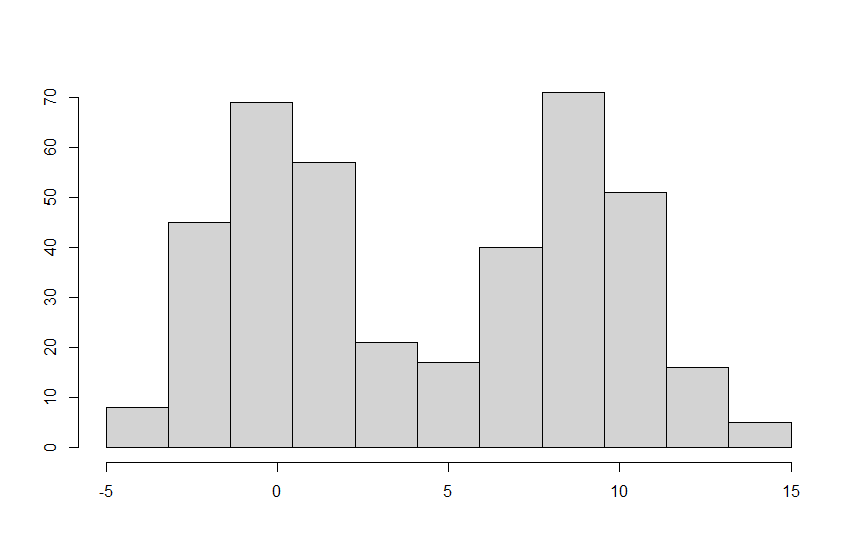
\includegraphics[width=10cm]{../fig/Cap02-DatosBimodales.png}
	\caption{Un conjunto de datos bimodal.}
	\label{cap02:fig:DatosBimodales}
    \end{figure}
El cálculo de la moda (o modas) es inmediato, a partir de las tablas de
frecuencias, y en los tutoriales comentaremos brevemente cómo realizarlo.

%\pendiente{Faltan ejemplos y un histograma bimodal para comparar con uno
%unimodal}

\section{Medidas de dispersión.}
\label{cap02:sec:MedidasDispersion}

%\subsection*{Introducción}

Hasta ahora hemos estado calculando {\em valores centrales}, que nos sirvieran
como buenos representantes de una colección de datos. Sin embargo, es fácil
entender que hay muchas colecciones de datos, muy distintas entre sí, que
pueden tener la misma media aritmética o la misma mediana, etcétera. El mismo
representante puede corresponder a colecciones de datos con {\em formas} muy
diferentes.

Por lo tanto, no sólo necesitamos un valor representativo, además necesitamos
una forma de medir {\em la calidad de ese representante.} ¿Cómo podemos hacer
esto? La idea que vamos a utilizar es la de \index{dispersión}{\sf dispersión}.
Una colección de números es poco dispersa cuando los datos están muy
concentrados alrededor de la media. Dicho de otra manera, si los datos son poco
dispersos, entonces se parecen bastante a la media (o al representante que
estemos usando). En una colección de datos poco dispersos, la {\em distancia
típica} de uno de los datos al valor central es pequeña.


Esa es la idea intuituiva, y como se ve está muy relacionada con el concepto de
{\em precisión} del que hablamos en la Sección
\ref{cap01:sec:PrecisionExactitudCifrasSignificativas} (ver la Figura
\ref{cap01:fig:PrecisionExactitud}, página
\pageref{cap01:fig:PrecisionExactitud}). Pero ahora tenemos que concretar mucho
más si queremos definir un valor de la dispersión que se pueda calcular. ¿cómo
podemos medir eso? En esta sección vamos a introducir varios métodos de medir
la dispersión de una colección de datos.

\subsection{Recorrido (o rango) y recorrido intercuartílico.}
\label{cap02:subsubsec:RangoIntercuartilico}

La idea más elemental de dispersión es la de \index{recorrido de una variable}{\sf recorrido}, que
ya hemos encontrado al pensar en las representaciones gráficas. El recorrido es simplemente la
diferencia entre el máximo y el mínimo de los valores. Es una manera rápida, pero excesivamente
simple, de analizar la dispersión de los datos, porque depende exclusivamente de dos valores (el
máximo y el mínimo), que pueden ser muy poco representativos. No obstante, es esencial, como primer
paso en el estudio de una colección de datos, empezar por calcular el recorrido, porque nos ayuda a
{\em enmarcar} nuestro trabajo, y evitar errores posteriores.

Un comentario sobre la terminología. El recorrido se denomina a veces, {\sf rango}\index{rango de
una variable}. Por razones que quedarán más claras en el Apéndice \ref{apendice:MasAlla}
(donde usaremos {\em rango} para otra noción distinta), nosotros preferimos el término {\em
recorrido} para este concepto. La confusión se debe a la traducción como {\em rango} de las dos
palabras inglesas {\em range}, que nosotros traducimos como {\em recorrido}, y {\em rank}, que
traducimos como {\em rango}.

Si queremos ir un paso más allá, para empezar a entender la forma de los datos, podemos usar las
medidas de posición. En concreto, la mediana y los cuartiles se pueden utilizar para medir la
dispersión de los datos, calculando el {\sf recorrido intercuartílico}\index{recorrido
intercuartílico} (en inglés, {\em interquartile range}, IQR) \index{IQR} \index{interquartile
range}, que se define como la diferencia entre el tercer y el primer cuartil.

        \begin{center}
            \fcolorbox{black}{Gris025}{\begin{minipage}{8cm}
            \begin{center}
            {\bf IQR, recorrido intercuartílico.}
            \end{center}
            El recorrido intercuartílico es:
            \[IQR=(\mbox{tercer cuartil}) - (\mbox{primer cuartil})\]
        \end{minipage}}
        \end{center}
\begin{ejemplo}
\label{cap02:ejem:IQR}
Para el conjunto de datos del Ejemplo \ref{cap02:ejem:MediaAritmetica02}, que eran estos:
\[9,\, 6,\, 19,\, 10,\, 17,\, 3,\, 28,\, 19,\, 3,\, 5,\, 19,\, 2,\, 150\]
el programa de ordenador (R, en este ejemplo) nos dice que el primer cuartil es $5$, y que el tercer cuartil es $19$. Por lo tanto,
\[IQR=19 - 5 = 14.\]
\qed
\end{ejemplo}

Los datos que son mucho menores que el primer cuartil o mucho mayores que el tercer cuartil se
consideran {\sf valores atípicos}\index{datos atípicos}\index{valores atípicos}\index{atípico} (en
inglés, {\em outlier})\index{outliers}. ¿Cómo de lejos tienen que estar de los cuartiles para
considerarlos {\em raros o excepcionales}? La forma habitual de proceder es considerar que {\sf un
valor mayor que el tercer cuartil, y cuya diferencia con ese cuartil es mayor que $1.5$ veces el
recorrido intercuartílico es un valor atípico}. De la misma forma, también es un valor atípico
aquel valor menor que el tercer cuartil, cuya diferencia con ese cuartil es mayor que
$1.5\cdot$IQR. Ya hemos discutido que existen muchas formas distintas de definir los cuartiles, así
que el recorrido intercuartílico depende, naturalmente, del método que se use para calcular los
cuartiles. Nosotros siempre lo calcularemos usando el ordenador (con R, la hoja de cálculo o algún
otro programa), y nos conformaremos con los valores por defecto que producen esos programas.

\begin{ejemplo}
\label{cap02:ejem:ValorAtipico}
Como habíamos anunciado, vamos a ver que, para el conjunto de datos del Ejemplo \ref{cap02:ejem:MediaAritmetica02}, el valor $150$ es un valor atípico. En el Ejemplo \ref{cap02:ejem:IQR} hemos visto que el tercer cuartil de esos valores era $19$, y que el recorrido intercuartílico era $14$. Así que un valor será atípico si es mayor que
\[\mbox{(tercer cuartil)}+1.5\cdot IQR=19 + 1.5 \cdot 14=19 + 21= 40.\]
Desde luego, queda claro que $150$ es un valor atípico, en ese conjunto.
\qed
\end{ejemplo}

La mediana, los cuartiles y el recorrido intercuartílico se utilizan para dibujar los diagramas
llamados de \index{diagrama de caja y bigotes} {\sf caja y bigotes} (en inglés,
{\em boxplot})\index{boxplot}, como el que se muestra en la Figura \ref{cap02:fig:Boxplot}. En estos
diagramas se dibuja una caja cuyos extremos son el primer y tercer cuartiles. Dentro de esa caja se
dibuja el valor de la mediana. Los valores atípicos se suelen mostrar como puntos individuales
(fuera de la caja, claro), y finalmente se dibujan segmentos que unen la caja con los datos más
alejados que no son atípicos.
    \begin{figure}[hp]
	\begin{center}
    (a)\\
	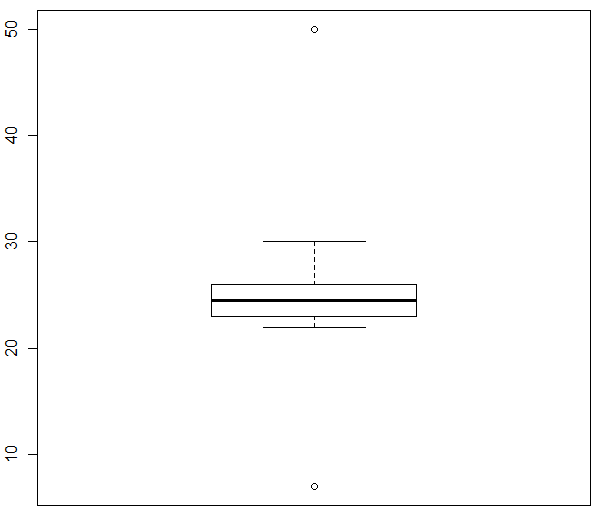
\includegraphics[width=9.5cm]{../fig/Cap02-BoxPlot.png}\\[3mm]
    (b)\\
    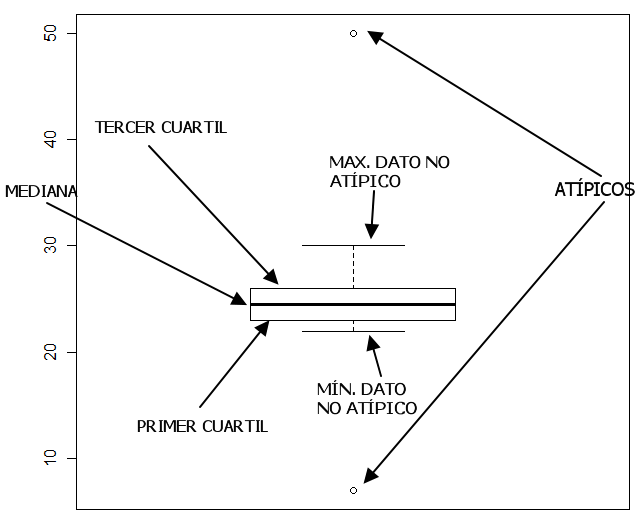
\includegraphics[width=10.5cm]{../fig/Cap02-BoxPlot-Estructura.png}
    \end{center}
	\caption{Un boxplot (a) y su estructura (b).}
	\label{cap02:fig:Boxplot}
    \end{figure}
Hasta hace muy poco, las hojas de cálculo no ofrecían la posibilidad de dibujar diagramas de cajas, y de hecho, nosotros recomendamos utilizar programas especializados para dibujarlos.
Aprenderemos a hacerlo en el Tutorial02, donde también veremos como calcular el recorrido
intercuartílico.

\subsection{Varianza y desviación típica.}
\label{cap02:subsec:VarianzaDesviacionTipica}

El recorrido intercuartílico se expresa en términos de cuartiles (o percentiles), y por lo tanto
tiene más que ver con la mediana que con la media aritmética. Sin embargo, uno de los objetivos más
importantes (si no el más importante) de la Estadística es hacer inferencias desde una muestra a la
población. Y cuando se trate de hacer inferencias, vamos a utilizar en primer lugar la media
aritmética como valor central o representativo de los datos. Por eso estas medidas de dispersión
relacionadas con la mediana, y no con la media, no son las mejores para hacer inferencia. {\sf
Necesitamos una medida de dispersión relacionada con la media aritmética.}

\subsubsection*{Varianza poblacional y cuasivarianza muestral.}


Tenemos, como siempre, un conjunto de $n$ datos,
\[x_1,x_2,\ldots,x_n\]
que corresponden a $n$ valores de una {\sf variable cuantitativa.} La primera
idea que se nos puede ocurrir es medir la diferencia entre cada uno de esos
valores y la media (la {\em desviación individual} de cada uno de los valores):
\[x_1-\bar x, x_2-\bar x,\ldots, x_n-\bar x,\]
Y para tener en cuenta la contribución de todos los valores podríamos pensar en hacer la media de estas desviaciones individuales:
\[\dfrac{(x_1-\bar x)+(x_2-\bar x)+\cdots+(x_n-\bar x)}{n}.\]
El problema es que esta suma siempre vale cero. Vamos a fijarnos en el numerador (y recuerda la definición de media aritmética):
\begin{equation}\label{cap02:ecu:SumaDesviacionesIgual0}
    (x_1-\bar x)+(x_2-\bar x)+\cdots+(x_n-\bar x)=(x_1+x_2+\cdots+x_n)-n\cdot\bar x=0.
\end{equation}
Está claro que tenemos que hacer algo más complicado, para evitar que el signo
de unas desviaciones se compense con el de otras. A partir de aquí se nos abren
dos posibilidades, usando dos operaciones matemáticas que eliminan el efecto de
los signos. Podemos usar el valor absoluto de las desviaciones individuales:
\[\dfrac{|x_1-\bar x|+|x_2-\bar x|+\cdots+|x_n-\bar x|}{n},\]
o podemos elevarlas al cuadrado:
\[\dfrac{(x_1-\bar x)^2+(x_2-\bar x)^2+\cdots+(x_n-\bar x)^2}{n}.\]
Las razones para elegir entre una u otra alternativa son técnicas: vamos a usar
la que mejor se comporte para hacer inferencias. Y, cuando se hacen inferencias
sobre la media, la mejor opción resulta ser la que utiliza los cuadrados. En
otros tipos de inferencia, no obstante, se usa la definición con el valor
absoluto.

La {\sf varianza (poblacional)} (o {\sf desviación cuadrática media})\index{varianza
(poblacional)}\index{desvici\'on cuadr\'atica media}\index{variance} (en ingl\'es, {\em variance})
del conjunto de datos $x_1,x_2,\ldots,x_n$ es:
        \begin{center}
        \fcolorbox{black}{Gris025}{
        \begin{minipage}{12cm}
                        \centering {\bf Varianza (poblacional)}
                        \begin{equation}\label{cap02:eq:varianzaPoblacional}
                    	  Var(x)=\dfrac{(x_1-\bar x)^2+(x_2-\bar x)^2+\cdots+(x_n-\bar x)^2}{n}=\dfrac{\displaystyle\sum_{i=1}^n(x_i-\bar x)^2}{n}.
                    	\end{equation}
        \end{minipage}}
        \end{center}
En muchos libros, incluso sin hablar de la varianza, se define una
cantidad relacionada, llamada {\sf varianza muestral} \index{varianza muestral}
o {\sf cuasivarianza muestral}, que es el nombre que nosotros vamos a usar,
\index{cuasivarianza muestral} mediante la fórmula
        \begin{center}
        \fcolorbox{black}{Gris025}{
        \begin{minipage}{12cm}
                        \centering {\bf Cuasivarianza muestral}
                        \begin{equation}\label{cap02:eq:cuasivarianzaMuestral}
                    	  s^2(x)=\dfrac{(x_1-\bar x)^2+(x_2-\bar x)^2+\cdots+(x_n-\bar x)^2}{\colorbox{lightgrey}{$n-1$}}=\dfrac{\displaystyle\sum_{i=1}^n(x_i-\bar x)^2}{\colorbox{lightgrey}{$n-1$}}.
                    	\end{equation}
        \end{minipage}}
        \end{center}
Como puede verse, la única diferencia es que en el denominador de la fórmula
aparece $n-1$ en lugar de $n$. En particular, si $n$ es muy grande, ambas
cantidades son prácticamente iguales, aunque la cuasivarianza siempre es
ligeramente mayor.

El concepto de cuasivarianza muestral será importante cuando hablemos de
inferencia, y entonces entenderemos el papel que juega la cuasivarianza
muestral, y su relación con la varianza (poblacional) tal como la hemos
definido. Lo que sí es {\sf\large muy importante}, usando software o
calculadoras, es que sepamos si el número que se obtiene es la varianza o la
cuasivarianza muestral.

\begin{ejemplo}
\label{cap02:ejem:Varianza}
Para el conjunto de valores
\[9,\, 6,\, 19,\, 10,\, 17,\, 3,\, 28,\, 19,\, 3,\, 5,\, 19,\, 2,\]
del Ejemplo \ref{cap02:ejem:MediaAritmetica} (pág. \pageref{cap02:ejem:MediaAritmetica}), que ya hemos usado en varios ejemplos, su media aritmética es:
\[\bar x=\dfrac{140}{12}\approx 11.67.\]
Así que la varianza (poblacional) es:
\[Var(x)=\dfrac{\left(9-\frac{140}{12}\right)^2+\left(6-\frac{140}{12}\right)^2+\cdots+\left(19-\frac{140}{12}\right)^2+\left(2-\frac{140}{12}\right)^2}{12}=\]
\[=\dfrac{\frac{2360}{3}}{12}=\dfrac{2360}{36}\approx 65.56\]
con cuatro cifras significativas. La cuasivarianza muestral se obtiene dividiendo por $11$ en lugar de $12$, y es:
\[s^2=\dfrac{\left(9-\frac{140}{12}\right)^2+\left(6-\frac{140}{12}\right)^2+\cdots+\left(19-\frac{140}{12}\right)^2+\left(2-\frac{140}{12}\right)^2}{11}=\]
\[=\dfrac{\frac{2360}{3}}{11}=\dfrac{2360}{33}\approx 71.52,\]
también con cuatro cifras significativas.

Dejamos como ejercicio para el lector comprobar que, para los datos del Ejemplo \ref{cap02:ejem:MediaAritmetica02}, que incluyen el valor atípico $150$, la varianza poblacional y la cuasivarianza muestral son (con cuatro cifras significativas)
\[
Var(x)\approx 1419,\quad s^2\approx 1538.
\]
Como puede verse, con la presencia del valor atípico la dispersión del conjunto ha aumentado mucho.
\qed
\end{ejemplo}

\subsubsection*{Varianza a partir de una tabla de frecuencias.}

Cuando lo que tenemos son datos descritos mediante una tabla de frecuencias,
debemos proceder así:
\begin{enumerate}
    \item La Ecuación \ref{cap02:eq:varianzaPoblacional} se sustituye por:
%        \begin{center}
%            \fcolorbox{black}{Gris025}{ \centering {\bf Varianza
%            (poblacional) a partir de una tabla de frecuencias}
%
%            \begin{minipage}{12cm}
%                \[v=Var(x)=\dfrac{\displaystyle\sum_{i=1}^k\colorbox{lightgrey}{$\bf f_i\cdot$}(x_i-\bar x)^2}
%        	        {\colorbox{lightgrey}{$\bf \displaystyle\sum_{i=1}^k f_i$}}.\]
%            \end{minipage}
%            }
%        \end{center}
        \begin{center}
        \fcolorbox{black}{Gris025}{
        \begin{minipage}{12cm}
                        \centering {\bf Varianza (poblacional) a partir de
            una tabla de frecuencias}
                        \[Var(x)=\dfrac{\displaystyle\sum_{i=1}^k\colorbox{lightgrey}{$\bf f_i\cdot$}(x_i-\bar x)^2}
        	        {\colorbox{lightgrey}{$\bf \displaystyle\sum_{i=1}^k f_i$}}.\]
        \end{minipage}}
        \end{center}





        donde, ahora, $x_1,\ldots,x_k$ son los valores {\em distintos} de la
        variable, y $f_1,\ldots,f_k$ son las correspondientes frecuencias.

    \item En el caso de datos agrupados por intervalos, los valores $x_i$
        que utilizaremos serán las marcas de clase.

\end{enumerate}
En los tutoriales tendremos ocasión sobrada de practicar este tipo de operaciones.


\subsubsection*{Desviación típica.}

La varianza, como medida de dispersión, tiene un grave inconveniente: puesto
que hemos elevado al cuadrado, las unidades en las que se expresa son
el cuadrado de las unidades originales en las que se medía la
variable $x$. Y nos gustaría que una medida de dispersión nos diera
una idea de, por ejemplo, cuantos metros se alejan de la media los
valores de una variable medida en metros. Dar la dispersión en metros
cuadrados es, cuando menos, extraño. Por esa razón, entre otras,
vamos a necesitar una nueva definición.

La {\sf desviación típica} \index{desviación típica} es la raíz
cuadrada de la varianza:
    \begin{center}
    \fcolorbox{black}{Gris025}{
    \begin{minipage}{12cm}
        {\centering \bf Desviación típica (poblacional)}
            \[DT(x)=\sqrt{Var(x)} =\sqrt{\dfrac{\displaystyle\sum_{i=1}^n(x_i-\bar x)^2}{n}}.\]
        Y, si es a partir de una tabla de frecuencias, entonces:
                        \[DT(x)=\sqrt{\dfrac{\displaystyle\sum_{i=1}^k\colorbox{lightgrey}{$\bf f_i\cdot$}(x_i-\bar x)^2}
        	        {\colorbox{lightgrey}{$\bf \displaystyle\sum_{i=1}^k f_i$}}}.\]
    \end{minipage}}
    \end{center}
También existe una {\sf cuasidesviación típica muestral $s$}, que es la
raíz cuadrada de la cuasivarianza muestral, y con la que nos volveremos a encontrar muchas veces en el resto del curso.

El cálculo de la desviación típica tiene las mismas características que el de la varianza. Y, de
nuevo, es \underline{\sf muy importante}, usando software o calculadoras, que sepamos si el número
que se obtiene es la desviación típica o la cuasidesviación típica muestral.

\begin{ejemplo}
Para los datos del Ejemmplo \ref{cap02:ejem:Varianza}, y tomando raíces cuadradas, se obtiene una desviación típica poblacional aproximadamente igual a $8.097$ y una cuasidesviación típica muestral aproximadamente igual a $8.457$.
\qed
\end{ejemplo}


\part{Probabilidad y variables aleatorias.}
\label{parte:ProbabilidadVariablesAleatorias}
% !Mode:: "Tex:UTF-8"

\section*{Introducción a la Probabilidad.}
\label{part02:intro}

\subsection*{Modelos. Fenómenos deterministas y aleatorios.}

Para poner todo lo que viene en perspectiva, nos vamos a detener unas líneas en la idea de {\sf
modelo}\index{modelo}. Básicamente, las ciencias intentan explicar los fen\'omenos que componen la
realidad, que suelen ser muy complicados, debido a la gran cantidad de elementos, muchas veces a
escalas muy distintas a las de nuestra experiencia cotidiana, que interactúan para producir el
resultado que observamos. Por eso resulta necesario hacer simplificaciones y descubrir las reglas
de funcionamiento elementales a partir de las que explicar el resto. Eso es básicamente un modelo:
una simplificación de la realidad, en la que conservamos los rasgos que consideramos esenciales,
para tratar de entender el fenómeno que estamos estudiando. A medida que se va entendiendo un
modelo, se añaden nuevos elementos que lo asemejan m\'as a la realidad. Desde el punto de vista de
la modelizaci\'on, hay dos grandes grupos de fen\'omenos:
\begin{itemize}
    \item Los {\sf fenómenos deterministas} \index{fen\'omeno determinista} son aquellos en los
        que, dadas unas condiciones iniciales, su evoluci\'on futura es totalmente predecible
        (est\'a determinada de antemano). Por ejemplo, cuando lanzamos un proyectil (en un modelo
        en el que despreciamos el rozamiento del aire, el efecto de la rotaci\'on de la 			
        tierra,\dots), una vez conocidas la velocidad con la que se lanza el proyectil y la
        inclinaci\'on respecto de la horizontal, podemos calcular a priori (esto es, predecir)
        con mucha precisión el alcance (a qu\'e distancia caer\'a), la altura m\'axima que
        alcanzar\'a,\dots.
    \item Un {\sf fen\'omeno aleatorio} \index{fen\'omeno aleatorio} 	es aquel que, dadas las
        condiciones iniciales, sabemos el conjunto de posibles resultados, pero no cu\'al de
        ellos suceder\'a. El lanzamiento de una moneda, un dado, el sexo de un hijo,\dots, son
        algunos ejemplos.
\end{itemize}
Pronto veremos que obtener una muestra de una poblaci\'on (si se hace bien) es un hecho
esencialmente aleatorio. Esto conlleva un cierto grado de incertidmyumbre (conocemos los posibles
resultados, pero no cu\'al de todos se realizar\'a) y la probabilidad es la herramienta adecuada
para lidiar con ella.

\subsection*{El papel de la Probabilidad en la Estadística.}

Hemos venido diciendo desde el principio del curso que el objetivo más importante de la Estadística
es realizar inferencias. Recordemos en que consiste esa idea: estamos interesados en estudiar un
fenómeno que ocurre en una determinada \index{poblaci\'on} {\sf población}. En este contexto,
población no se refiere sólo a seres vivos. Si queremos estudiar la antigüedad del parque móvil de
España, la población la forman todos los vehículos a motor del país (cada vehículo es un
individuo). Si queremos estudiar la dotación tecnológica de los centros de secundaria, la población
la forman todos los institutos, y cada instituto es un individuo de esa población. En general,
resulta imposible, indeseable o inviable estudiar uno por uno todos los individuos de la población.
Por esa razón, lo que hacemos es obtener información sobre una {\sf muestra} de la población. Es
decir, un subconjunto de individuos de la población original, de los que obtenemos información
sobre el fenómeno que nos interesa.

Tenemos que distinguir por lo tanto, en todo lo que hagamos a partir de ahora, qué afirmaciones se
refieren a la población (la colección completa) y cuáles se refieren a la muestra. Los únicos datos
a los que realmente tendremos acceso son los de la muestra (o muestras) que hayamos obtenido. La
muestra nos proporcionará datos sobre alguna variable (o variables) relacionadas con el fenómeno
que estamos estudiando. Es decir, que podemos empezar pensando que en la muestra tenemos, como en
todo lo que hemos hecho hasta ahora un conjunto de $n$ datos,
        \[x_1,x_2,\ldots,x_n.\]

En el ejemplo del parque móvil, podríamos haber obtenido las fichas técnicas de 1000 vehículos (la
población completa consta de cerca de 28 millones de vehículos\footnote{En concreto, 27963880,
según datos de un informe de Anfac del año 2010 (ver enlace  [\,\ref{enlace0000}\,]\label{enlace0000a}) .}). Y una variable que nos puede interesar
para estudiar la antigüedad del parque móvil es el año de matriculación. Así que tendríamos 1000
valores $x_1,\ldots,x_{1000}$, donde cada uno de esos valores representa la antigüedad (en años) de
un vehículo. Con esos 1000 valores podemos calcular una media, que llamaremos la \index{media
muestral} {\sf media muestral}:
    \[\bar x=\dfrac{x_1+x_2+\cdots+x_{1000}}{1000}\]
Naturalmente, si accediéramos a {\em todos} los datos, nos encontraríamos con una lista {\em mucho}
más larga, de alrededor de 28 millones de números:
    \[m_1,m_2,m_3,\ldots,m_{27963880}.\]
Y podríamos hacer la media de todos estos datos, que llamaremos la \index{media poblacional}{\sf
media poblacional}:
    \[\mu=\dfrac{m_1+m_2+m_3+\ldots+m_{27963880}}{27963880}.\]
Los símbolos que hemos elegido no son casuales. Vamos a utilizar siempre $\bar x$ para referirnos a
la media muestral y $\mu$ (la letra griega mu) para referirnos a la media poblacional. Este es un
convenio firmemente asentado entre los usuarios de la Estadística.

Naturalmente, hacer esta media poblacional es mucho más difícil, complicado, caro, etcétera. Y ahí
es donde aparece la idea de inferencia, que se puede formular aproximadamente así, en un sentido
intuitivo:
    \begin{center}
        \fcolorbox{black}{Gris025}{\begin{minipage}{11cm}
            {\sf Si hemos seleccionado esos 1000 coches al \colorbox{lightgrey}{\bf azar} de
            entre los aproximadamente 28 millones posibles, entonces es muy
            \colorbox{lightgrey}{\bf probable} que la media muestral $\bar x$  se parezca mucho a la
            media poblacional

            $\mu$.}
        \end{minipage}}
    \end{center}
    Hemos destacado en esta frase las palabras azar y probable, porque son la justificación de lo que
    vamos a estar haciendo en los próximos capítulos. Para poder usar la Estadística con rigor
    científico, tenemos que entender qué quiere decir exactamente {\em seleccionar al azar}, y cómo
    se puede {\em medir la probabilidad} de algo. Para esto necesitamos el lenguaje matemático de la
    Teoría de la Probabilidad.

\subsection*{El lenguaje de la Probabilidad.}

La probabilidad nació entre juegos de azar, y sus progenitores incluyen una larga estirpe de
truhanes, fulleros y timadores, junto con algunas de las mentes matemáticas más brillantes de su
época. De esa mezcla de linajes sólo cabía esperar una teoría llena de sorpresas, paradojas,
trampas, cosas que parecen lo que no son... la Probabilidad es muy bonita, y no es demasiado fácil.
De hecho, puede ser muy difícil, y elevarse en grandes abstracciones. Pero le garantizamos al
lector que, como dijimos en la Introducción del libro, vamos a hacer un esfuerzo para hacerle las cosas tan simples como sea posible (y ni un poco más simples).

Una de las razones que, a nuestro juicio, hacen que la Probabilidad resulte más difícil, es que,
sea por razones evolutivas o por cualesquiera  otras razones, el hecho es que los humanos tenemos
una intuición relativamente pobre a la hora de juzgar sobre la probabilidad de distintos
acontecimientos. Por poner un ejemplo, por comparación, nuestra intuición geométrica es bastante
mejor. Pero cuando se trata de evaluar probabilidades, especialmente cuando se trata de sucesos
poco frecuentes, nuestra intuición, en general, nos abandona, y debemos recurrir a las matemáticas
para pisar tierra firme.

A esa dificultad, se suma el hecho de que el nivel matemático del curso va a elevarse en esta
parte, en la que vamos a recurrir, en el Capítulo \ref{cap:Probabilidad} a la Combinatoria, y en el
Capítulo \ref{cap:VariablesAleatorias} al lenguaje de las funciones y del Cálculo. En particular,
necesitaremos la integración. No suponemos que el lector sepa integrar, así que hemos tratado de
incluir, en el Capítulo \ref{cap:VariablesAleatorias}, un tratamiento tan autocontenido del tema
como nos ha sido posible. Afortunadamente, buena parte de la parte más mecánica (y tediosa) de la
integración se puede dejar ahora en manos de los ordenadores. Así que, de la misma forma que ya
nadie piensa en aprender a usar una tabla de logaritmos, hemos adoptado la postura de, llegado el
momento, pedir al lector que use el ordenador para calcular tal o cual integral. Esa delegación de los detalles técnicos en las máquinas nos deja libres para concentrarnos en las ideas, que son siempre la parte importante. Aspiramos a que el lector empiece a entender {\em para que sirve} la integral, aunque no sepa calcular ninguna a mano. Por seguir con la analogía, los logaritmos se calculan con las máquinas, pero eso no nos exime de entender sus propiedades y, sobre todo, cuando y cómo pueden sernos útiles. 

El Capítulo \ref{cap:TeoremaCentralLimite} marca la transición, en la que salimos de la
Probabilidad, para tomar el camino que lleva a la Inferencia, de vuelta a Estadística. Este
capítulo, y los dos siguientes, son, como hemos dicho, la parte central del curso, donde se
establecen las ideas fundamentales de la Estadística clásica.


\chapter{Probabilidad.}
\label{cap:Probabilidad}
% !Mode:: "Tex:UTF-8"

\section{Primeras nociones sobre Probabilidad.}
\label{cap03:sec:PrimerasNocionesProbabilidad}
\label{PrimerasNocionesProbabilidad}


El estudio de la Probabilidad nació, como disciplina científica, en el siglo XVII y en relación con los juegos de azar y las apuestas. Y es en ese contexto, de lanzar monedas, y de juegos con dados, cartas y ruletas, donde todavía se siguen encontrando la mayoría de los ejemplos con los que se presenta la teoría a quienes se inician en su estudio. Nosotros vamos a hacer lo mismo.
    \begin{enumerate}
        \item Lanzamiento de dados: cuando se lanzan unos dados (sin trucar), el resultado de cada lanzamiento individual es imposible de predecir. Se observa, tras realizar un número muy grande de lanzamientos, que cada uno de los seis posibles resultados aparece aproximadamente una sexta parte de las veces.
        \item Lanzamiento de monedas: del mismo modo, cuando se lanza una moneda (sin trucar), se observa, al cabo de muchos lanzamientos, que cada uno de los dos posibles resultados aparece aproximadamente la mitad de las veces.
        \item Las loterías, con la extracción de bolas numeradas de una urna o un bombo giratorio; o la ruleta, en la que la bola que se lanza puede acabar en cualquiera de las 36 (o 37) casillas.  Estos juegos y otros similares, ofrecían ejemplos adicionales con elementos comunes a los anteriores.
    \end{enumerate}
Las apuestas, basadas en esos juegos de azar, y los casinos son, desde antiguo, un entretenimiento muy apreciado. Para hacer más interesante el juego, la humanidad fue construyendo otros juegos combinados más complicados. Por ejemplo, apostamos cada uno un euro y lanzamos dos dados: si la suma de los resultados es par, yo me llevo los dos euros. Si es impar, los ganas tú. La pregunta es evidente ¿Es este un juego {\em justo} para ambos jugadores? En concreto, lo que queremos saber es: si jugamos muchas, muchas veces ¿cuántos euros perderé o ganaré yo en promedio por cada euro invertido? ¿Y cuántos ganarás o perderás tú? Está claro que para que un jugador esté dispuesto a participar, y a arriesgar su fortuna, y desde luego para que alguien considere rentable el casino como negocio, o la lotería como forma de recaudar dinero, es preciso ofrecerle {\sf información precisa sobre cuáles son las ganancias esperadas del juego}. Uno de nuestros objetivos es aprender a responder a esa pregunta: ¿cómo se calculan las ganancias esperadas? No es una pregunta tan específica de los juegos de azar como pueda parecer a primera vista. En general, cuando nos enfrentamos a un fenómeno aleatorio, ¿cuáles son los resultados esperables? ¿Cómo podemos hacer medible nuestra incertidumbre sobre esos resultados?
        
\subsubsection*{}
Otra cosa que la humanidad constató rápidamente al tratar con los juegos de azar es que, como hemos
dicho en la introducción a esta parte del curso, nuestra intuición, en este terreno, es
especialmente débil. Las personas en general, tendemos a subestimar o sobrevalorar mucho las
probabilidades de muchos fenómenos. Y así consideramos como milagros algunos fenómenos
perfectamente normales y predecibles, o viceversa. Uno de nuestros ejemplos favoritos de lo
engañosa que puede ser nuestra intuición cuando se trata de probabilidades, es el que se conoce
como {\sf problema de Monty Hall}\index{problema de Monty Hall}\index{Monty Hall, problema de},
sobre el que puedes leer en el enlace [\,\ref{enlace0004}\,]\label{enlace0004a}.
En el Episodio 13 de la primera temporada de la serie de televisión Numb3rs (más información en el
enlace [\,\ref{enlace0005}\label{enlace0005a}\,]),  se ilustra
este problema de una forma muy entretenida. Recomendamos encarecidamente al lector que, si tiene
ocasión, no deje de ver ese fragmento en particular.
%
%en esta clase vamos a ver un vídeo de un fragmento  de la serie de televisión \link{http://en.wikipedia.org/wiki/Numb3rs}{Numb3rs} en el que se describe  En Moodle tenéis un enlace al vídeo por si queréis volver a verlo.\\[3mm]

Otro ejemplo pertinente, que además tiene interés histórico, es el que se describe en detalle (y
con humor) en el Capítulo 3 del libro {\em La Estadística en Comic} de Gonick y Smith (ver
referencia \cite{EstadisticaComic} de la Bibliografía), como {\sf Problema del Caballero de
Méré}\index{Méré, problema del caballero de}\index{Caballero de Méré, problema de}\index{problema
del caballero de Méré} (más información en el enlace [\,\ref{enlace0006}\,].\label{enlace0006a}): ¿qué
es más probable?
    \begin{itemize}
    \item[(a)] obtener al menos un seis en cuatro tiradas de un dado, o
    \item[(b)] obtener al menos un seis doble en 24 tiradas de dos dados?
    \end{itemize}
    Los jugadores que, en aquella época, se planteaban esta pregunta respondían inicialmente así:
    \begin{itemize}
    \item[(a)] La probabilidad de obtener un seis en cada tirada es $\dfrac{1}{6}$. Por lo tanto, en cuatro tiradas es 
    \[\dfrac{1}{6}+\dfrac{1}{6} = \dfrac{1}{3}.\]

    \item[(b)] La probabilidad de obtener un doble seis en cada tirada de dos dados es $\dfrac{1}{36}$, porque hay 36 resultados distintos, y todos aparecen con la misma frecuencia. Por lo tanto, en veinticuatro tiradas será \[\dfrac{1}{36}+\cdots+\dfrac{1}{36}=\dfrac{24}{36}=\dfrac{2}{3}.\]
    \end{itemize}
Así que en principio ambas apuestas son iguales, y las cuentas parecen indicar que recuperaríamos dos de cada tres euros invertidos (el 66\%). Sin embargo, no es así, como algunos de esos jugadores debieron experimentar dolorosamente en sus patrimonios.

Uno de nuestros objetivos en este curso es animar al lector a que ponga a prueba sus ideas, y considere a la Estadística, en buena medida, como una ciencia {\em experimental}. Eso es posible en muchos casos recurriendo al ordenador. Por esa razón, en el Tutorial03 vamos a ver cómo podemos usar el ordenador para simular un gran número de partidas de las dos apuestas del Caballero de Méré. Repetimos que la ganancia esperada es de un 66\% de lo invertido. Y lo que se observa es que la proporción de apuestas perdidas frente a apuestas ganadas no es, ni la que esperábamos, ni siquiera es igual en ambos casos. De hecho, dentro de poco vamos a aprender a calcular los valores correctos, y veremos que para la apuesta (a) ese valor es aproximadamente $0.52$, mientras que para la apuesta (b) es aproximadamente $0.49$.
%
%
%Para ilustrar lo que decimos, vamos a utilizar aquí dos hojas de cálculo, llamadas \fichero{../datos/Cap03-DeMere1.ods}{{Cap03-DeMere1.ods}} (para la apuesta (a)) y \fichero{../datos/Cap03-DeMere2.ods}{{Cap03-DeMere2.ods}} (para la apuesta (b))\label{cap03:lugar:hojasCalculoDeMere}, en las que hemos {\em simulado} esas dos apuestas, y hemos jugado 1000 veces cada una de ellas.


\section{Regla de Laplace.}
\label{cap03:sec:ReglaLaplace}

Lo que tienen en común todas las situaciones que hemos descrito, ligadas a juegos de azar, es que:
        \begin{enumerate}
            \item Hay una lista de resultados individuales posibles: los seis números que aparecen en las caras de un dado, las dos caras de la moneda, las 36 casillas de la ruleta francesa, etc. Estos resultados se llaman {\sf resultados elementales}.
            \item Si repetimos el experimento muchas veces (muchos millones de veces si es
                necesario), y observamos los resultados, comprobamos que la {\em frecuencia
                relativa} de aparición de cada uno de los resultados elementales es la misma para
                todos ellos: $1/6$ para cada número en el dado, $1/2$ para cada cara de la
                moneda, $1/36$ para cada casilla de la ruleta. En ese caso decimos que los
                sucesos elementales son \index{sucesos equiprobables}{\sf
                equiprobables}\footnote{Aunque, en la realidad, las cosas no son tan sencillas.
                Quizá os resulte interesante buscar en Internet información sobre la relación
                entre la ruleta y la familia Pelayo.}.
        \end{enumerate}

En este contexto, Pierre Simon Laplace\index{Laplace} (más información sobre él en el enlace
[\,\ref{enlace0003}\label{enlace0003a}\,]),
uno de los mayores genios matemáticos de la Ilustración francesa, desarrolló la que seguramente es
la primera contribución verdaderamente científica al análisis de la Probabilidad, y que en su honor
se conoce como \index{regla de Laplace}{\sf Regla de Laplace.} Vamos a fijar el lenguaje necesario
para formular esa regla.
    \begin{itemize}
        \item[(a)]  Estamos interesados en un {\sf fenómeno o experimento aleatorio}. Es decir, que sucede al azar; como lanzar una moneda, un dado o un par de dados, etc. Y suponemos que ese experimento tiene $n$ {\sf resultados elementales} diferentes:
            \[\{a_1,a_2,\ldots,a_n,\}\]
            y que esos resultados elementales son {\sf equiprobables}, en el sentido de la igualdad de las frecuencias relativas que hemos descrito, cuando el experimento se repite muchas veces.

        \item[(b)]  Además, definimos un {\sf suceso aleatorio}, llamémoslo $A$, que es un resultado, posiblemente más complejo, que se puede definir en términos de los resultados elementales del experimento en (a). Por ejemplo, si lanzamos un dado, $A$ puede ser: obtener un número par. O, si lanzamos dos dados, $A$ puede ser: que la suma de los números sea divisible por $5$. En cualquier caso, en algunos de los resultados elementales ocurre $A$ y en otros no. Eso permite pensar en $A$ como un {\sf subconjunto del conjunto de resultados elementales}. Y aquellos resultados elementales en los que se observa $A$ se dice que son {\sf resultados favorables} al suceso $A$. Por ejemplo, si lanzamos un dado, los resultados favorables al suceso $A=$ {\em(obtener un número par)} son $\{2,4,6\}$. Y podemos decir, sin riesgo de confusión, que $A=\{2,4,6\}$.
    \end{itemize}

Con estas premisas, la formulación de la Regla de Laplace es esta:
        \begin{center}
        \fcolorbox{black}{Gris025}{
        \begin{minipage}{12cm}
            \centering {\bf Regla de Laplace}\\
            La probabilidad del suceso A es el cociente:
            \begin{equation}
            \label{cap03:ecu:ReglaLaplace}
            P(A)=\dfrac{\mbox{número de sucesos elementales favorables a $A$}}{\mbox{número total de sucesos elementales}}
            \end{equation}
        \end{minipage}}
        \end{center}
%
%
%
%
%
%
%    \begin{center}
%        \fbox{\colorbox{Gris025}{
%        \begin{minipage}{13cm}
%    \begin{center}
%        {\bf Regla de Laplace: } \\[3mm]
%                \end{center}
%        La probabilidad del suceso A es el cociente:
%        \[p(A)=\dfrac{\mbox{número de sucesos elementales favorables a $A$}}{\mbox{número total de sucesos elementales}}
%        \]
%        \end{minipage}}
%        }
%    \end{center}
La Regla de Laplace supuso un impulso definitivo para la teoría de la Probabilidad, porque hizo posible comenzar a calcular probabilidades y obligó a los matemáticos, a la luz de esos cálculos, a pensar en las propiedades de la probabilidad. Además, esa regla se basa en el recuento de los casos favorables al suceso $A$ de entre todos los posibles. Y eso obliga a desarrollar técnicas de recuento a veces extremadamente sofisticadas (contar es algo muy difícil, aunque parezca paradójico), con lo que la Combinatoria se vio también favorecida por esta Regla de Laplace.

Precisamente, es esa enorme complejidad de algunas operaciones en la Combinatoria, la que produce las mayores dificultades técnicas asociadas al uso de la Regla de Laplace. En este curso no nos queremos entretener con ese tema más allá de lo imprescindible. Pero, como muestra y anticipo, podemos dar una respuesta en términos de combinatoria al problema del caballero De Méré.  Para ello tenemos que pensar en:
    \begin{center}
    \begin{minipage}{11cm}
      {\sf\em El conjunto de todos los resultados elementales posibles del experimento ``lanzar cuatro veces un dado''.}
    \end{minipage}
    \end{center}
Esto, para empezar, puede resultar complicado. Como estrategia, es más fácil empezar por pensar en el caso de lanzar dos veces el dado, y nos preguntamos por la probabilidad del suceso:
    \begin{center}
    \begin{minipage}{11cm}
      {\sf  $A=${\em obtener al menos un seis en las dos tiradas.} }
    \end{minipage}
    \end{center}
Como principio metodológico, esta técnica de entender primero bien una versión {\em a escala reducida} del problema es un buen recurso, al que conviene acostumbrarse. La respuesta de la {\em probabilidad ingenua} a este problema sería, simplemente:

{\sf\em La probabilidad de obtener un seis en cada tirada es $\dfrac{1}{6}$. Por lo tanto, en dos tiradas es %\[\dfrac{1}{6}+\dfrac{1}{6}+\dfrac{1}{6}+\dfrac{1}{6}=\dfrac{2}{3}.\]}
\[\dfrac{1}{6}+\dfrac{1}{6} = \dfrac{1}{3}.\]}
Si, por contra, queremos aplicar la Regla de Laplace al experimento de lanzar dos veces seguidas un dado, debemos empezar por dejar claro cuáles son los sucesos elementales equiprobables de este experimento. Los resumimos en esta tabla:
    \[
        \rowcolors{6}{lightgrey}{lightgrey}
        \begin{array}{rrrrrr}
        (1,1)&(1,2)&(1,3)&(1,4)&(1,5)&\cellcolor[gray]{0.9}{(1,6)}\\
        (2,1)&(2,2)&(2,3)&(2,4)&(2,5)&\cellcolor[gray]{0.9}{(2,6)}\\
        (3,1)&(3,2)&(3,3)&(3,4)&(3,5)&\cellcolor[gray]{0.9}{(3,6)}\\
        (4,1)&(4,2)&(4,3)&(4,4)&(4,5)&\cellcolor[gray]{0.9}{(4,6)}\\
        (5,1)&(5,2)&(5,3)&(5,4)&(5,5)&\cellcolor[gray]{0.9}{(5,6)}\\
        \cellcolor[gray]{0.9}{(6,1)}&\cellcolor[gray]{0.9}{(6,2)}&\cellcolor[gray]{0.9}{(6,3)}&\cellcolor[gray]{0.9}{(6,4)}&\cellcolor[gray]{0.9}{(6,5)}&\cellcolor[gray]{0.9}{(6,6)}
        \end{array}
    \]
Observa que:
    \begin{itemize}
        \item El primer número del paréntesis es el resultado del primer lanzamiento, y el segundo número es el resultado del segundo lanzamiento.
        \item Hay, por tanto, $6\cdot 6=36$ sucesos elementales equiprobables.
        \item El suceso $(1,2)$ y el $(2,1)$ (por ejemplo), son distintos (y equiprobables).
        \item Hemos señalado en la tabla los sucesos elementales que son favorables al suceso $A=${\em obtener al menos un seis en las dos tiradas}. Y hay exactamente 11 de estos.
    \end{itemize}
Así pues, la Regla de Laplace predice en este caso un valor de $\frac{11}{36}$, frente a los $\frac{12}{36}$ de la probabilidad ingenua (como la que
hemos aplicado antes). En el Tutorial03 podrás comprobar experimentalmente que la Regla de Laplace es mucho mejor que la probabilidad ingenua a la hora de predecir el
resultado.

Con la Regla de Laplace se pueden analizar también, usando bastante más maquinaria combinatoria, los dos experimentos (a) y (b) del apartado \ref{PrimerasNocionesProbabilidad} (pág. \pageref{PrimerasNocionesProbabilidad}). Volveremos sobre esto en la Sección \ref{cap03:sec:Combinatoria} (ver página \pageref{cap03:subsubsec:JuegosDeMereCombinatoria}).
%Aquí dejamos simplemente un \textattachfile{../fig/DeMere2a.html}{\textcolor{blue}{documento}}  (se abre en el navegador y requiere Java) con los valores combinatorios necesarios para ese cálculo.

Cerramos este apartado con un ejemplo-pregunta, que deberías responder antes de seguir adelante.

\begin{Ejemplo}\label{Cap03:ejem:CualEsProbabilidadSumaDosDadosIgualASiete}
    ¿Cual es la probabilidad de que la suma de los resultados al lanzar dos dados sea igual a siete? Sugerimos usar la tabla de 36 resultados posibles que acabamos de ver en esta sección.
\end{Ejemplo}



%\section*{Tareas asignadas para esta sesión.}
%
%\begin{enumerate}
%   \item En la clase de hoy hemos descrito un juego de apuestas basado en el lanzamiento de dos dados, y nos hemos preguntado si era justo. En concreto, nos preguntamos cuáles son las ganancias esperadas para cada uno de los jugadores. En Moodle tienes una tarea esperándote, en la que debes responder a esa pregunta.
%\end{enumerate}




%\setcounter{section}{0}
%\section*{\fbox{\colorbox{Gris025}{{Sesiones 8, 9, 10. Probabilidad.}}}}
%
%\subsection*{\fbox{\colorbox{Gris025}{{Calculando probabilidades.}}}}
%\subsection*{Fecha: Jueves, 13/10/2011, 16h. También viernes 14/10 y martes 18/10.}
%
%\noindent{\bf Este fichero pdf lleva adjuntos los ficheros de datos necesarios.}
%
%%\subsection*{\fbox{1. Ejemplos preliminares }}
%\setcounter{tocdepth}{1}
%%\tableofcontents
%\section*{Lectura recomendada}
%
%Las mismas de la sesión anterior.


\section{Probabilidad más allá de la Regla de Laplace.}
\label{cap03:sec:ProbabilidadMasAllaReglaLaplace}

La Regla de Laplace puede servir, con más o menos complicaciones combinatorias, para calcular probabilidades en casos como los de los dados, la
ruleta, las monedas, etcétera. Pero desde el punto de vista teórico, hay una dificultad, que el lector probablemente ya ha detectado: en la base de
esa Regla de Laplace está la idea de {\em sucesos equiprobables}. Así que puede que la regla de Laplace sirviera para {\em calcular} probabilidades, y
hacer la discusión más precisa. Y ese es, sin duda, su mérito histórico. Pero no parece una buena forma de {\em definir} Probabilidad, al menos, si
queremos evitar incurrir en una {\em definición circular}, usando la noción de probabilidad para definir la propia idea de probabilidad. Además, incluso sin salir del casino, ¿qué sucede cuando los dados están cargados o las monedas
trucadas? Y en el mundo real es muy fácil encontrar ejemplos, en los que la noción de sucesos equiprobables no es de gran ayuda a la hora de calcular
probabilidades: el mundo está lleno de ``dados cargados'' en favor de uno u otro resultado. Y como vamos a ver en los siguientes ejemplos, esa
definición resulta claramente insuficiente para afrontar algunas situaciones.

\begin{itemize}
\item Por ejemplo, cuando tomamos una bombilla de una cadena de montaje y la
inspeccionamos para determinar si es defectuosa o no, parece natural pensar que esos dos ($A=$``bombilla defectuosa'' y $\bar A=$``bombilla no defectuosa'') son los sucesos elementales. De hecho, tratar de introducir otros sucesos ``más elementales'', seguramente complicaría excesivamente el análisis.  Pero, desde luego, lo \'ultimo que esperar\'iamos (o al menos el propietario de la f\'abrica) es que los sucesos $A$ y $\bar{A}$  fueran equiprobables.
En casos como este se utiliza la {\sf definici\'on frecuentista de probabilidad}
\index{definici\'on frecuentista de probabilidad}. En este contexto, la soluci\'on pasa
por observar durante cierto tiempo la producci\'on y asignar a los eventos $A$ y $\bar{A}$ una probabilidad igual a la frecuencia relativa observada (de ah\'i el nombre).

\item Podríamos pensar que esa definición frecuentista es la respuesta definitiva. Sin embargo, para poder aplicarla,  es necesario suponer que los sucesos puedan repetirse
una cantidad grande de veces, para medir las frecuencias correspondientes. Se ha apuntado muchas veces que ese enfoque frecuentista tropieza con muchas dificultades conceptuales: ¿qué quiere decir {\em repetir un suceso}, cuando las circunstancias, necesariamente, habrán cambiado? En el caso del cálculo de la probabilidad de que mañana llueva, ¿qué querría decir ``repetir el día de mañana''? Y la alternativa más extendida es el {\sf enfoque Bayesiano} de la Estadística, que entiende la probabilidad como una medida de nuestro {\em grado de certidumbre} en la posibilidad de que un suceso ocurra, o nuestra estimación de la {\em verosimilitud} de ese suceso. En cualquier caso, no queremos que esa discusión conceptual nos haga perder el paso aquí. La discusión tiene sentido, desde luego, pero sólo cuando se han entendido los elementos básicos del problema, que es a lo que nos vamos a dedicar en este curso. En los Comentarios a la Bibliografía (pág. \pageref{apendice:comentarioBibliografia}) daremos alguna indicación más sobre este tema.


\end{itemize}

Lo anterior pone de manifiesto que
\begin{itemize}
	\item La noci\'on de probabilidad es ciertamente escurridiza.
	\item Posiblemente necesitemos un marco m\'as o menos abstracto para abarcar
		todas las situaciones en las que aparece la idea de probabilidad.
\end{itemize}



\subsection{Definición (casi) rigurosa de probabilidad.}
\label{Cap03:def:DefinicionProbabilidad}



Iniciamos esta secci\'on con algunos ejemplos que motivar\'an lo que viene a continuaci\'on:

\begin{Ejemplo}\label{Cap03:ejem:LanzamientoMonedaHastPrimeraCara}
Por ejemplo, siguiendo en el terreno de los juegos de azar: dos jugadores A y B, juegan a lanzar una moneda. El primero que saque cara, gana, y empieza lanzando $A$. ¿Cuál es la probabilidad de que gane A?
Si tratamos de aplicar la Regla de Laplace a este problema nos tropezamos con una dificultad; no hay límite al número de lanzamientos necesarios en el juego. Al tratar de hacer la lista de ``casos posibles'' nos tenemos que plantear la posibilidad de encontrarnos con secuencias de cruces cada vez más largas.
    \[
        \smiley, \dag\smiley, \dag \dag\smiley, \dag \dag \dag\smiley, \dag \dag \dag \dag\smiley,\ldots
    \]
Así que si queremos asignar probabilidades a los resultados de este juego, la Regla de Laplace no parece de gran ayuda.\qed
\end{Ejemplo}


Otro problema con el que se enfrentaba la teoría de la probabilidad al aplicar la Regla de Laplace
era el caso de la asignación de probabilidades a experimentos que involucran variables continuas. Veamos un ejemplo ilustrativo.
\begin{ejemplo}
\label{cap03:ejem:ProbabilidadGeometricaElegirPuntoIntervalo}
Si en el intervalo $[0,1]$ de la recta real elegimos un número $x$ al azar (de manera que todos los valores de $x$ sean igual de probables), ¿cuál es la probabilidad de que sea $1/3\leq x\leq 2/3$?

¿Qué te dice (a gritos) la intuición? Y ahora trata de pensar en este problema usando la regla de Laplace. ¿Cuántos casos posibles (valores de $x$) hay? ¿Cuántos son los casos favorables?

La intuición nos dice que la probabilidad de que el punto $x$ pertenezca al intervalo $[0,1/3]$ es igual a $1/3$, que es precisamente la {\em longitud} de ese intervalo. Vamos a tratar de acercarnos, con las herramientas que tenemos, a la idea de elegir un punto al azar en el intervalo $[0, 1]$. Una posible manera de hacerlo sería considerar muchos puntos del intervalo. Vamos a tomar $n_0=100000$, y consideremos los $n_0+1=100000+1$ puntos repartidos de forma homogénea por todo el intervalo, que podemos definir de esta forma:
\[
\dfrac{0}{100000}, \dfrac{1}{100000}, \dfrac{2}{100000},\dfrac{3}{100000},\,\ldots\,,
\dfrac{99998}{100000},\dfrac{99999}{100000},\dfrac{100000}{100000}.
\]
¿Ves por qué son $100000 + 1$? O, para un valor $n_0$ general, pensamos en los puntos:
\[\dfrac{0}{n_0}, \dfrac{1}{n_0}, \dfrac{2}{n_0}, \,\ldots\,
,\dfrac{n_0-2}{n_0},\dfrac{n_0-1}{n_0},\dfrac{n_0}{n_0},\]
Y ahora elegimos uno de esos puntos al azar, y miramos si pertenece al intervalo $[0, 1/3]$.  La Figura \ref{Cap03:fig:EjemploProbabilidadGeometricaElegirPuntoIntervalo} trata de ilustrar esta idea (con muchos menos de $100000$ puntos).

    \begin{figure}[h]
	\centering
	\begin{enColor}
	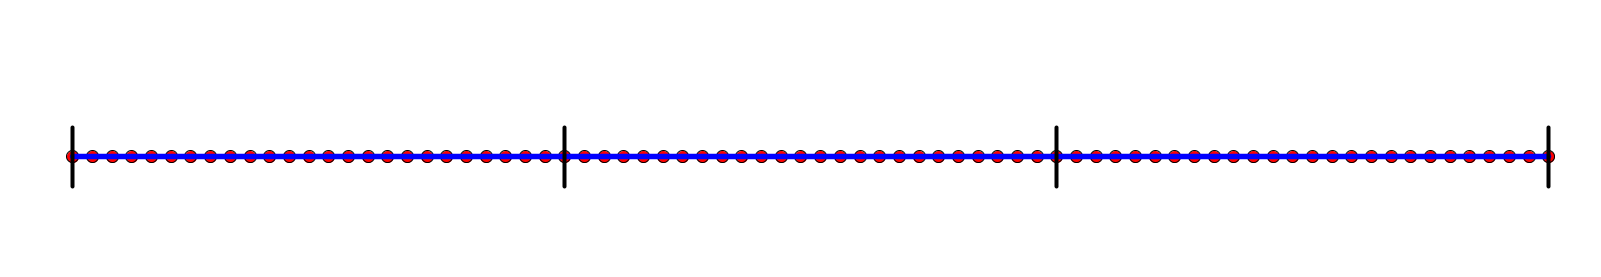
\includegraphics[width=12cm]{../fig/Cap03-EjemploProbabilidadGeometrica01.png}
	\end{enColor}
	\begin{bn}
	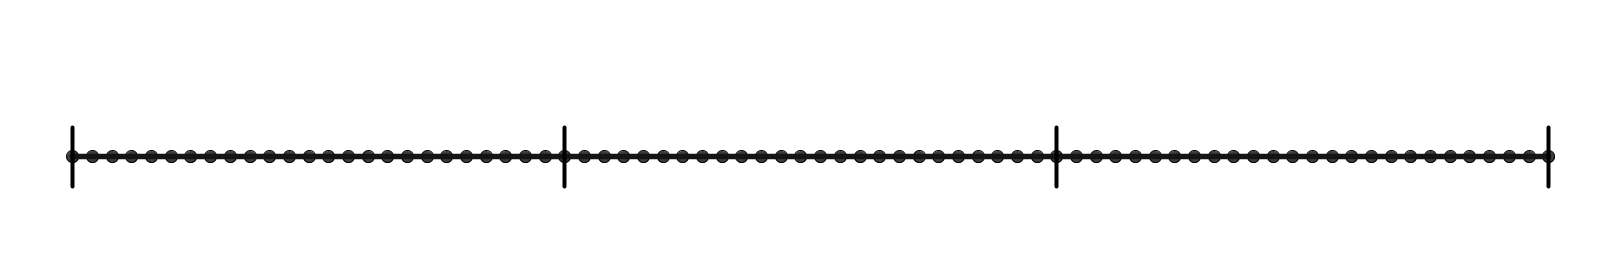
\includegraphics[width=12cm]{../fig/Cap03-EjemploProbabilidadGeometrica01-bn.png}
	\end{bn}
	\caption{Si elegimos uno de esos puntos al azar, ¿cuál es la probabilidad de que pertenezca al
    segmento situado más a la derecha?}
    \label{Cap03:fig:EjemploProbabilidadGeometricaElegirPuntoIntervalo}
    \end{figure}
Aquí sí que podemos usar la regla de Laplace, para concluir que, puesto que (muy aproximadamente) la tercera parte de esos puntos pertenecen al intervalo, la probabilidad que buscamos debe ser $1/3$. Una manera alternativa de pensar en esto, sin recurrir a la regla de Laplace, consiste en pensar que elegimos no ya uno, sino muchos de entre esos $n_0+1$ puntos, y estudiamos la {\em proporción} de puntos que pertenecen al intervalo $[0,1/3]$. Está intuitivamente claro que esa proporción se parecerá mucho a $1/3$. Además, la aproximación a $1/3$ es tanto mejor cuanto mayor sea $n_0$. En el Tutorial03 trataremos de justificar usando el ordenador lo que la intuición nos está diciendo para este caso.

Naturalmente, el problema con el enfoque que hemos usado en este ejemplo es que en el intervalo $[0,1]$ hay infinitos puntos, distintos de esos $n_0$ puntos que hemos seleccionado. Así que, por más grande que sea $n_0$, la lista de puntos que podemos elegir dista mucho de la idea teórica de ``cualquier punto del intervalo [0,1]''. Por eso este procedimiento no resulta del todo satisfactorio desde el punto de vista teórico. Sin embargo, es una idea interesante y que puede ayudar a guiar nuestra intuición. Por eso merece la pena explorarla, como vamos a hacer en otros ejemplos.
\qed
\end{ejemplo}
La pregunta que hemos discutido en este ejemplo es representativa del tipo de problemas que genéricamente se llaman de {\em Probabilidad Geométrica}. En este caso, en el que elegimos puntos de un segmento, se trata de un problema unidimensional.
%Y un
%ejemplo similar: en una circunferencia de radio 1 se eligen dos puntos al azar. ¿Cuál es la
%longitud media de la cuerda de circunferencia que definen? Esta pregunta es un ejemplo del tipo de
%problemas que genéricamente se llaman de {\em Probabilidad Geométrica}. El fichero GeoGebra
%\begin{center}
% \fichero{../datos/Cap03-ProbabilidadGeometrica01.ggb}{Cap03-ProbabilidadGeometrica01.ggb}
%\end{center}
% ilustra este problema. Para ver otro ejemplo famoso, recomendamos
%visitar la página web de construcciones con GeoGebra de Manuel Sada (en la dirección web
%\link{http://docentes.educacion.navarra.es/msadaall/geogebra}{docentes.educacion.navarra.es/msadaall/geogebra/}),
%donde entre otras muchas cosas interesantes, podéis ver una ilustración de varios problemas
%clásicos de la Probabilidad como el {\em Problema de la aguja de Buffon}, o el {\em
%Problema de Monty Hall}, del que ya hemos hablado.
Vamos a ver ahora otro  ejemplo de probabilidad geométrica, en este caso bidimensional, que nos va a ayudar a seguir avanzando, y sobre el que volveremos varias veces más adelante.
\begin{Ejemplo}
\label{Cap03:ejem:ProbabilidadGeometricaMontecarlo}
Supongamos que tenemos un cuadrado de lado 4 y en su interior dibujamos cierta figura $A$. Para fijar ideas, $A$ puede ser un un círculo de radio 1, centrado en el cuadrado, como en la Figura \ref{Cap03:fig:Circulo}.
    \begin{figure}[h]
	\centering
	\begin{enColor}
% 	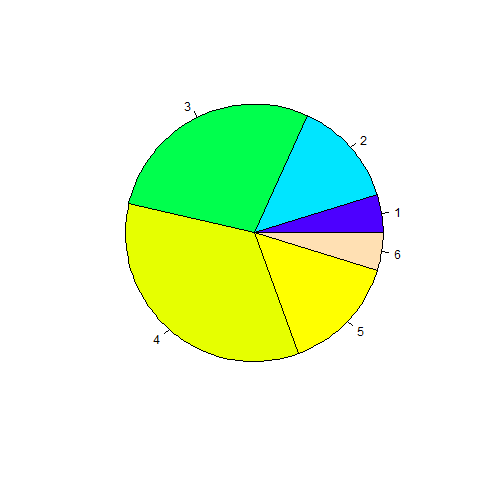
\includegraphics[height=6cm]{../fig/Cap01-DiagramaSectores.png}
% 	\hspace{0.5cm}
	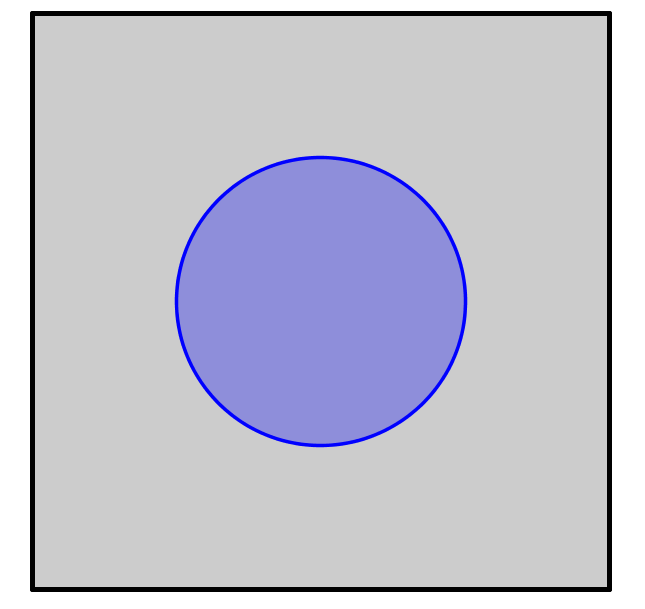
\includegraphics[height=5cm]{../fig/Cap03-Montecarlo.png}
	\end{enColor}
	\begin{bn}
% 	\includegraphics[height=6cm]{../fig/Cap01-DiagramaSectores-bn.png}
% 	\hspace{0.5cm}
	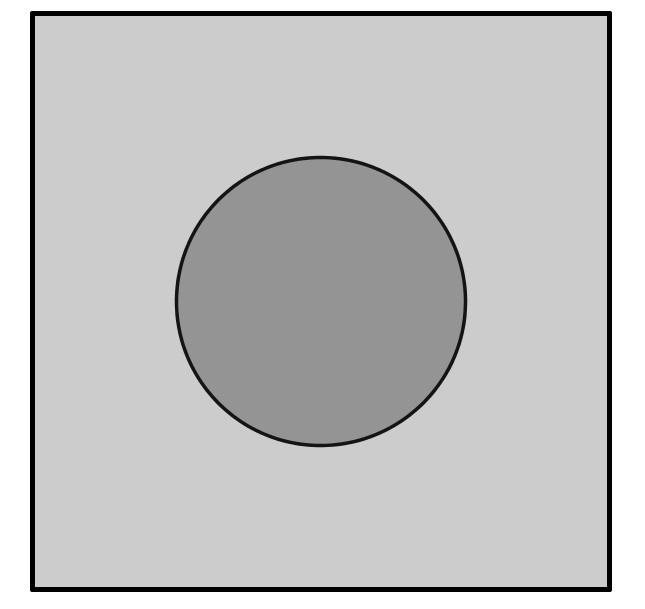
\includegraphics[height=5cm]{../fig/Cap03-Montecarlo-bn.png}
	\end{bn}
	\caption{C\'irculo de radio $1$ centrado en un cuadrado de lado $4$.}\label{Cap03:fig:Circulo}
    \end{figure}
Si tomamos un punto al azar dentro del cuadrado ¿cuál es la probabilidad de que ese punto caiga dentro del círculo $A$?  En el Ejemplo \ref{Cap03:fig:EjemploProbabilidadGeometricaElegirPuntoIntervalo} elegíamos un punto al azar del segmento $[0,1]$, y aquí elegimos un punto al azar en el cuadrado de lado $4$. Una buena manera de pensar en esto es imaginarse que lanzamos un dardo al cuadrado, pero que el lanzamiento es completamente al azar, de manera que  ``todos los puntos del cuadrado son {\em equiprobables}''. Si nos imaginamos que, en lugar de un dardo, lanzamos miles de ellos, ¿qué proporción de esos dardos caerían dentro del círculo (serían {\em favorables} al círculo)? La intuición indica que esa proporción depende del área del círculo. El círculo es la diana, y cuanto más grande sea el área de la diana, más probable será acertar. Esta relación nos permite apreciar una relación entre la idea de probabilidad y la idea de área, que nos resulta mucho más intuitiva. Este vínculo entre área y probabilidad es extremadamente importante. En el Tutorial03 usaremos el ordenador para explorar esta relación más detenidamente.

Hemos entrecomillado la frase anterior sobre la equiprobabilidad de los puntos, porque ahí está el conflicto fundamental que hace que ejemplos como este sean imposibles de reconciliar con la regla de Laplace. En cualquier región del cuadrado hay infinitos puntos. En particular, el círculo contiene infinitos puntos. Si todos esos puntos del círculo tienen la misma probabilidad, distinta de cero, entonces por muy pequeña que sea, aunque sea una billonésima, cuando sumemos un trillón de puntos obtendremos... desde luego, más de uno. Así que no podemos tener estas cosas a la vez:
\begin{enumerate}
    \item los puntos son equiprobables.
    \item su probabilidad es distinta de cero.
    \item la probabilidad es un número entre 0 y 1 que se calcula, como en la regla de Laplace, sumando las probabilidades de los puntos individuales.
\end{enumerate}
Para salir de este atolladero, necesitamos, en ejemplos como este, una forma radicalmente distinta de pensar la probabilidad.
\qed
\end{Ejemplo}
¿Cuál es esa forma distinta de pensar la probabilidad? Los ejemplos anteriores nos dan la clave. Debería quedar claro, al pensar detenidamente sobre estos ejemplos, que la noción de probabilidad y la noción de área de una figura plana tienen muchas propiedades en común (en los problemas unidimensionales, en lugar del área usamos la longitud).  El problema con el que se encontraron los matemáticos, claro está, es que la propia noción teórica de área es igual de complicada de definir que la Probabilidad. Esto puede resultar un poco sorprendente, porque, a diferencia de lo que sucede con la probabilidad, el área resulta una idea intuitiva. De hecho, es engañosamente fácil de entender.
\begin{ejemplo}
\label{cap03:ejem:TrianguloSierpinski}
Para ver un ejemplo en el que la noción de área empieza a resultar resbaladiza, podemos pensar en la construcción del llamado {\em triángulo de Sierpinski}\index{triángulo de Sierpinski} (ver el enlace [\,\ref{enlace0002}\label{enlace0002a}\,]). Este conjunto se construye mediante un proceso iterativo, mediante una serie de operaciones que se repiten ``infinitas veces'' (técnicamente, por un paso al límite). Las primeras etapas de la construcción se ilustran en la Figura \ref{Cap03:fig:TrianguloSierpinski}.
\begin{figure}[b!]
\begin{center}
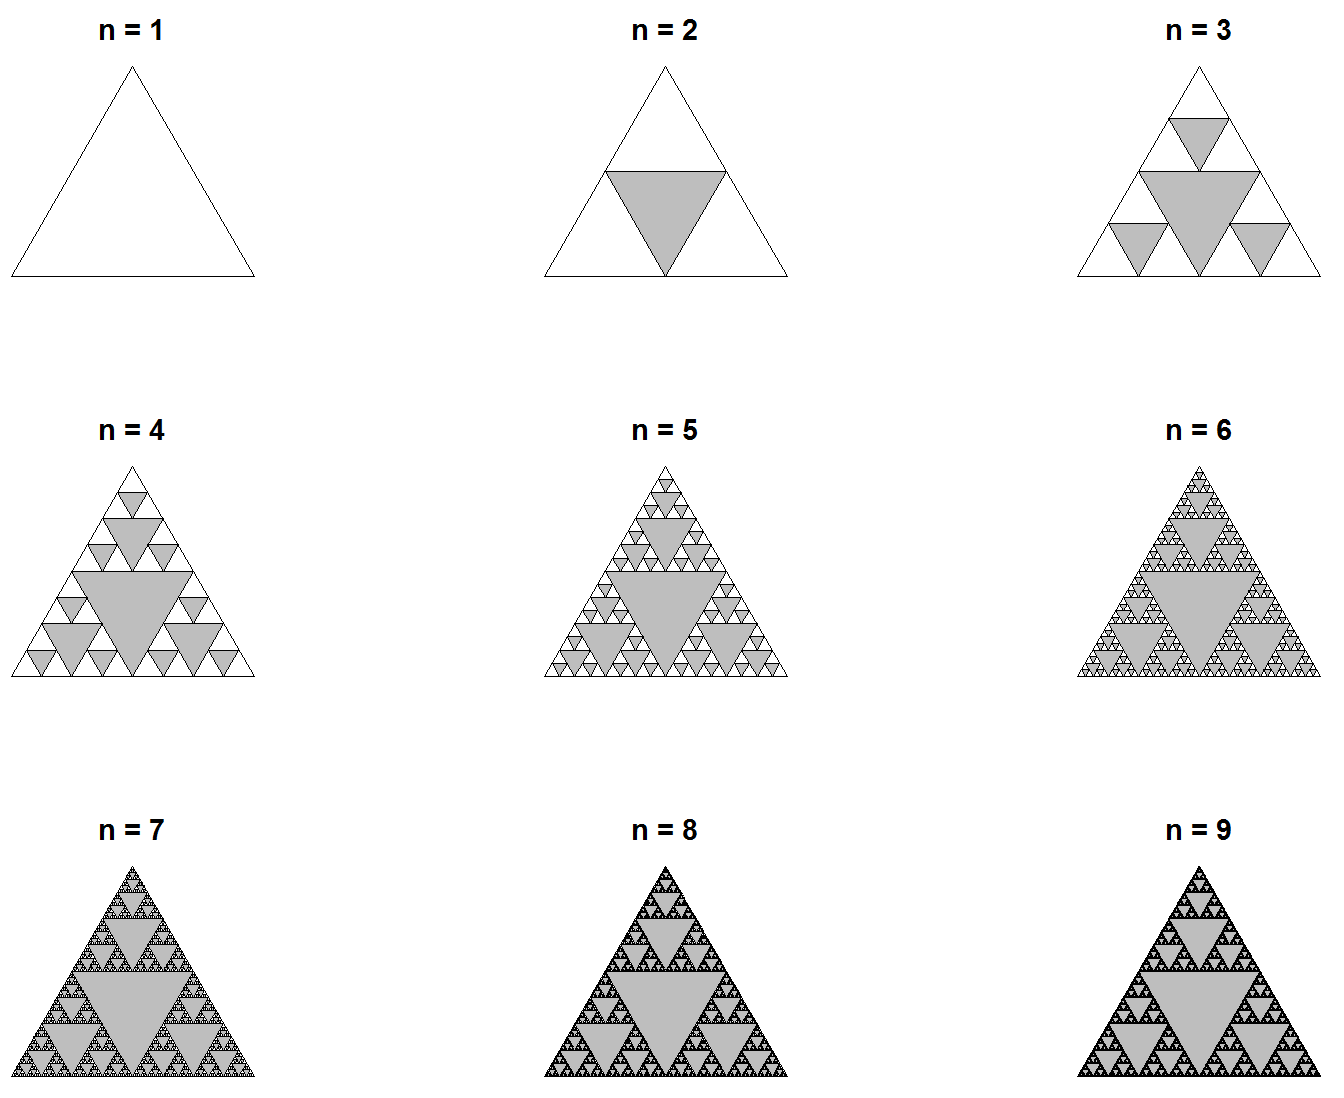
\includegraphics[width=14cm]{../fig/Cap03-SierpinskiConR.png}
\caption{Las primeras etapas en la construcción del triángulo de Sierpinski}
\label{Cap03:fig:TrianguloSierpinski}
\end{center}
\end{figure}
Como se ve en esa figura, el punto de partida ($n=1$) es un triángulo equilátero. Inicialmente consideramos todos los puntos del triángulo (borde e interior). En la siguiente etapa ($n=2$), {\em eliminamos} del conjunto los puntos del triángulo central sombreado, de manera que lo que queda son los tres triángulos equiláteros, copias a escala del original. En el siguiente paso ($n=3$), aplicamos la misma operación (``eliminar el triángulo central'') a cada uno de los triángulos que conservamos en la fase $n=2$. Y así vamos procediendo, aplicando esa misma operación en cada paso para pasar de $n$ a $n+1$. El Triángulo de Sierpinski es el conjunto de puntos que quedan ``al final'' de este proceso. De alguna manera, es un conjunto formado por ``infinitos triángulos infinitamente pequeños''.
\qed
\end{ejemplo}
%\begin{center}
%  \fichero{../datos/Cap03-Sierpinski.ggb}{Cap03-Sierpinski.ggb},
%\end{center}
%que ilustra los primeros pasos en la construcción de la figura llamada {\em el triángulo de Sierpinski}\index{triángulo de Sierpinski}, que se obtiene como límite siguiendo el proceso que ilustra ese fichero.\qed
Los entrecomillados del final de este ejemplo indican que esas son descripciones informales. Y ese es precisamente el problema con el que se encontraron los matemáticos a finales del siglo XIX: no resultaba nada fácil encontrar una manera formal, rigurosa, de definir conceptos como el área para figuras como esta (y otras mucho más complicadas). A causa de estos, y otros problemas similares, los matemáticos de aquella época (y entre ellos, muy destacadamente, Andréi Kolmogórov; más información sobre él en el enlace [\,\ref{enlace0001}\label{enlace0001a}\,])\label{enlace0001a}
construyeron una {\em Teoría Axiomática de la Probabilidad}. Aquí no podemos entrar en todos los
detalles técnicos, que son complicados, pero podemos decir que, esencialmente, se trata de lo siguiente:
    \begin{itemize}
        \item[(A)] Inicialmente tenemos un \index{espacio muestral}{\sf espacio muestral} $\Omega$, que representa el conjunto de todos los posibles resultados de un experimento.
        \item[(B)] Un \index{suceso aleatorio}{\sf suceso aleatorio} es un subconjunto del espacio muestral. Esta es la parte en la que vamos a ser menos rigurosos. En realidad, no todos los subconjuntos sirven, por la misma razón que hemos visto al observar que no es fácil asignar un área a todos los subconjuntos posibles. Pero para entender qué subconjuntos son sucesos y cuáles no, tendríamos que definir el concepto de $\sigma$-álgebra\index{$\sigma$-álgebra}\index{sigma álgebra}, y eso nos llevaría demasiado tiempo. Nos vamos a conformar con decir que hay un {\em tipo especial de subconjuntos}, los sucesos aleatorios, a los que sabemos asignarles una probabilidad.
        \item[(C)] La \index{función Probabilidad}{\sf Función Probabilidad}, que representaremos con una letra $P$,  esuna función o regla que  asigna un cierto número $P(A)$ a cada suceso aleatorio $A$ del espacio muestral $\Omega$. Y esa función probabilidad debe cumplir  tres propiedades, que aparecen más abajo. Antes de enunciarlas, necesitamos una aclaración sobre la notación que aparece en la segunda propiedad  de la probabilidad: el \index{suceso unión}\index{unión}{\sf suceso unión} $A_1\cup A_2$ significa que suceden $A_1$ o $A_2$ (o ambos a la vez). El \index{suceso intersección}\index{intersección}{\sf suceso intersección} $A_1\cap A_2$ significa que $A_1$ y $A_2$ ocurren ambos simultáneamente. A menudo se usan diagramas (de Venn), como el de la Figura \ref{Cap03:fig:DiagramaVennInterseccionSucesos},para representar, conceptualmente, las uniones o intersecciones de sucesos.

\begin{figure}[htbp]
\begin{center}
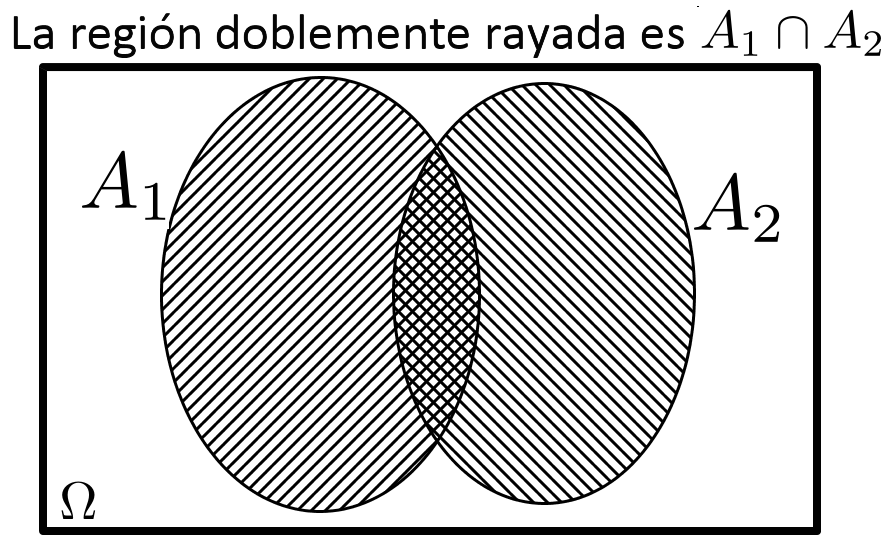
\includegraphics[height=4cm]{../fig/Cap03-DiagramaVennInterseccionSucesos.png}
	\caption{Diagrama para la intersección de dos sucesos }\label{Cap03:fig:DiagramaVennInterseccionSucesos}
\end{center}
\end{figure}

            En un diagrama como ese, el rectángulo exterior representa el espacio muestral, y cada una de las figuras rayadas que aparecen, de forma elíptica,  representa un suceso. En este caso, la elipse de la izquierda se corresponde con $A_1$ y la de la derecha con $A_2$. La intersección $A_1\cap A_2$ es la zona común a ambas elipses. En cambio, la unión $A_\cup A_2$ sería la zona total que cubren las dos elipses, conjuntamente.

            Con esa notación, las propiedades de la Probabilidad son estas:
            \begin{center}
            \fcolorbox{black}{Gris025}{
            \begin{minipage}{12cm}
                \centering {\bf Propiedades fundamentales de la Función Probabilidad:}
                \label{cap03:def:PropiedadesFundamentalesFuncionProbabilidad}
                \index{probabilidad, propiedades fundamentales}
                \begin{enumerate}
                    \item Sea cual sea el suceso aleatorio $A$, siempre se cumple que $0\leq P(A)\leq 1$.
                        \item Si $A_1$ y $A_2$ son \index{sucesos aleatorios disjuntos}\index{disjuntos} sucesos aleatorios disjuntos, es decir si $A_1\cap A_2=\emptyset$ (esto equivale a decir que es imposible que $A_1$ y $A_2$ ocurran a la vez) entonces
                            \[P(A_1\cup A_2)=P(A_1)+P(A_2).\]
                            En el caso $A_1\cap A_2=\emptyset$ también diremos que los sucesos son {\sf incompatibles}.\index{sucesos incompatibles}\index{incompatibles, sucesos}
                        \item La probabilidad del espacio muestral completo es $1$. Es decir, $P(\Omega)=1$.
                \end{enumerate}
            \end{minipage}}
            \end{center}
    \end{itemize}
La Figura \ref{Cap03:fig:DiagramaVennSucesosDisjuntos} representa, en un diagrama conceptual, el caso de dos sucesos incompatibles (o disjuntos).

\begin{figure}[htbp]
\begin{center}
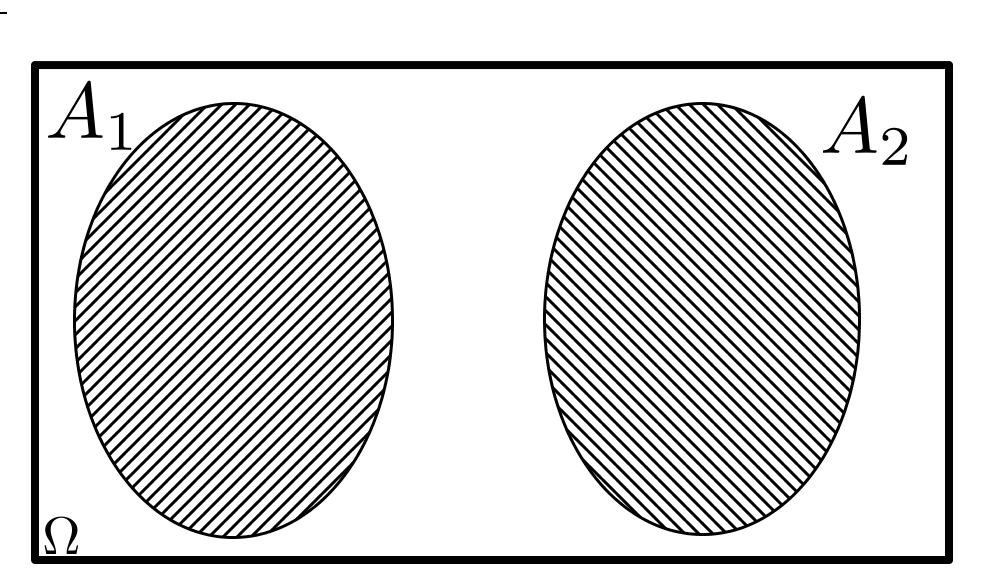
\includegraphics[height=4cm]{../fig/Cap03-DiagramaVennSucesosDisjuntos.png}
	\caption{Diagrama para la intersección de dos sucesos }\label{Cap03:fig:DiagramaVennSucesosDisjuntos}
\end{center}
\end{figure}

La forma en la que se asignan o {\sf distribuyen} las probabilidades define el \index{modelo probabilístico}{\sf modelo probabilístico} que utilizamos en cada problema. Por ejemplo, la Regla de Laplace es el modelo probabilístico típico que usamos en situaciones como las de los juegos de azar que hemos descrito, y en general, cuando, basados en nuestra experiencia, podemos suponer la existencia de una familia de sucesos elementales equiprobables. En los problemas de probabilidad geométrica adoptamos, a menudo (pero no siempre), un modelo probabilístico que consiste en suponer que la probabilidad de una región es proporcional a su área. \\

Vamos a ver como se aplican estas ideas al ejemplo del lanzamiento de una moneda hasta la primera cara que vimos antes.
\begin{Ejemplo}[\bf Continuación del Ejemplo \ref{Cap03:ejem:LanzamientoMonedaHastPrimeraCara}, pág. \pageref{Cap03:ejem:LanzamientoMonedaHastPrimeraCara}]\label{cap03:ejem:LanzamientoMonedaHastPrimeraCara:2}

En este caso, podemos definir un modelo de probabilidad así. El espacio muestral $\Omega$ es el conjunto de todas las listas de la forma
\[a_1=\smiley, a_2=\dag\smiley, a_3=\dag \dag\smiley,\ldots,a_k=\hspace{-7pt}\overbrace{\dag \dag \dag \cdots\dag \dag \dag }^{(k-1)\mbox{ cruces }}\hspace{-7pt}\smiley,\ldots\]
es decir, $k-1$ cruces hasta la primera cara. Fíjate en que este espacio muestral tiene infinitos elementos. Todos los subconjuntos se consideran sucesos aleatorios, y para definir la probabilidad decimos que:
\begin{enumerate}
    \item $P(a_k)=P(\overbrace{\dag \dag \dag \cdots\dag \dag \dag }^{k-1\mbox{ cruces }}\hspace{-5pt}\smiley)=\dfrac{1}{2^{k}}$,
    \item Si $A=\{a_i\}$ es un suceso aleatorio, es decir, $A$ es un conjunto de listas de cruces y caras, entonces $P(A)=\sum P(a_i)$. Dicho de otro
modo, la probabilidad de un conjunto de listas es igual a la suma de las probabilidades de las listas que lo forman\footnote{No vamos a entretenernos
en comprobar que, con esta definición, se cumplen las tres propiedades fundamentales, pero le garantizamos al lector que, en efecto, así es.}. Es
decir, que si
        \[A=\{a_1,a_3,a_6\}=\{\smiley,\,\dag \dag\smiley\, ,\, \dag \dag \dag \dag \dag\smiley\,\},\]
        entonces
        \[P(A)=P(a_1)+P(a_3)+P(a_6)=\dfrac{1}{2}+\dfrac{1}{2^3}+\dfrac{1}{2^6}.\]
\end{enumerate}
Ahora podemos calcular la probabilidad de que gane la persona que empieza lanzando. Ese suceso es:
\[A=\{a_1,a_3,a_5,a_7,\ldots\}=\mbox{el primer jugador gana en la $k$-ésima jugada},\]
y por lo tanto su probabilidad es:
\[P(A)=\underbrace{P(a_1)+P(a_3)+P(a_5)+P(a_7)+\cdots}_{\mbox{listas de longitud impar}}=
\dfrac{1}{2}+\dfrac{1}{2^3}+\dfrac{1}{2^5}+\dfrac{1}{2^7}+\cdots=\dfrac{2}{3}.
\]
Esta última suma la hemos calculado usando el hecho de que se trata de la suma de una {\sf progresión geométrica} de razón $\dfrac{1}{2^2}$. No podemos entretenernos en explicar cómo se hacen este tipo de sumas infinitas (series), pero sí queremos tranquilizar al lector, asegurándole que las progresiones geométricas son las más fáciles de todas. En el Tutorial03 veremos cómo se puede usar el ordenador para calcular algunas sumas como estas.\qed
\end{Ejemplo}

Este enfoque también sirve para los problemas-ejemplo de probabilidad geométrica que hemos discutido antes. Esencialmente, lo que hay que tener presente es que la definición de Función Probabilidad está relacionada con el área, y el único matiz importante es que un área puede ser arbitrariamente grande o pequeña (por lo tanto, puede ser cualquier número positivo), mientras que una probabilidad viene obligada a ser un número entre 0 y 1. La forma natural de hacer esto es fijar de antemano cierta figura geométrica $\Omega$, que es el espacio muestral, y definir la probabilidad de un  suceso $A$ como
\[P(A)=\dfrac{\mbox{área de }A}{\mbox{área de }\Omega}.\]
En el Ejemplo \ref{Cap03:ejem:ProbabilidadGeometricaMontecarlo}, la probabilidad de un suceso (subconjunto del cuadrado grande) es igual al área de ese suceso dividida por 16 (el área del cuadrado grande). {\sf Un punto o una recta son sucesos de probabilidad cero} (porque no tienen área). Esta última propiedad resulta un poco chocante a los recién llegados al mundo de la Probabilidad, pero no lo es tanto si se piensa en términos de áreas. {La originalidad (y genialidad) de la idea de Kolmogórov es que se conserva la propiedad de la aditividad de la probabilidad (la propiedad (2)), a cambio de pequeñas ``paradojas'' aparentes, como esta de que los puntos {\em individualmente considerados} tienen todos probabilidad cero, pero el {\em conjunto de (infinitos) puntos} tiene probabilidad no nula. Insistimos, esto sólo parece una paradoja hasta que se piensa en términos de área, y en ese momento nos damos cuenta de que con el área sucede exactamente lo mismo. ¿Qué queda entonces de esa idea de equiprobabilidad ingenua, en la que decíamos que todos los puntos del cuadrado son equiprobables? Lo que queda es una versión al menos igual de intuitiva, pero mucho más coherente: todas las regiones del cuadrado {\em del mismo área} son equiprobables.}

Y una última aclaración: la probabilidad definida mediante la Regla de Laplace cumple, desde luego, las tres propiedades fundamentales que hemos enunciado. Lo que hemos hecho ha sido {\em generalizar} la noción de probabilidad a otros contextos en los que la idea de favorables/posibles no se aplica. Pero los ejemplos que se basan en la Regla de Laplace son a menudo un buen ``laboratorio mental'' para poner a prueba nuestras ideas y nuestra comprensión de las propiedades de las probabilidades.

\subsection{Más propiedades de la Función Probabilidad.}
\label{cap03:subsec:MasPropiedadesFuncionProbabilidad}

Las tres propiedades básicas de la Función Probabilidad tienen una serie de consecuencias que vamos a explorar en el resto de este capítulo. Las primeras y más sencillas aparecen resumidas en este cuadro:	
    \begin{center}
    \fcolorbox{black}{Gris025}{
    \begin{minipage}{12cm}
        \centering {\bf Propiedades adicionales de la Función Probabilidad:}
         \begin{enumerate}
            \item Sea cual sea el suceso aleatorio $A$, si $A^c$ es el
            \index{suceso complementario}\index{complementario} {\sf suceso complementario o suceso contrario}\index{suceso contrario}\index{contrario}
            (es decir ``no ocurre $A$'') siempre se cumple que
            \[P(A^c)=1-P(A).\]
            \item La probabilidad del\index{suceso vacío} {\sf suceso vacío}
            $\emptyset$ es $0$; es decir \[P(\emptyset)=0.\]
            \item Si $A\subset B$, (se lee: si $A$ es un subconjunto de $B$,
            es decir si siempre que ocurre $A$ ocurre $B$), entonces
            \[P(A)\leq P(B)\mbox{, y además }P(B)=P(A)+P(B\cap A^c).\]
            \item Si $A_1$ y $A_2$ son sucesos aleatorios cualesquiera,
            \begin{equation}\label{cap03:ecu:ProbabilidadUnionDosSucesosCasoGeneral}
                P(A_1\cup A_2)=P(A_1)+P(A_2)-P(A_1\cap A_2).
            \end{equation}
        \end{enumerate}
    \end{minipage}}
    \end{center}
La última de estas propiedades se puede generalizar a $n$ sucesos aleatorios. Veamos como queda para tres, y dejamos al lector que imagine el resultado general {\em (ojo a los signos)}:
    \[\begin{array}{l}
    P(A_1\cup A_2\cup A_3)=\\
    =\underbrace{\left(P(A_1)+P(A_2)+P(A_3)\right)}_{\mbox{tomados de 1 en 1}}\colorbox{lightgrey}{\bf -}\underbrace{\left(P(A_1\cap A_2)+P(A_1\cap A_3)+P(A_2\cap A_3)\right)}_{\mbox{tomados de 2 en 2}}\\
    \colorbox{lightgrey}{\bf +}\underbrace{\left(P(A_1\cap A_2\cap A_3)\right)}_{\mbox{tomados de 3 en 3}}.
    \end{array}
    \]
La Figura \ref{Cap03:fig:DiagramaVennUnioTresSucesos} ilustra esta propiedad. Los sucesos intersección dos a dos corresponden a las zonas doblemente rayadas de la figura, y la intersección tres a tres corresponde a la parte central, triplemente rayada.

\begin{figure}[h!]
\begin{center}
    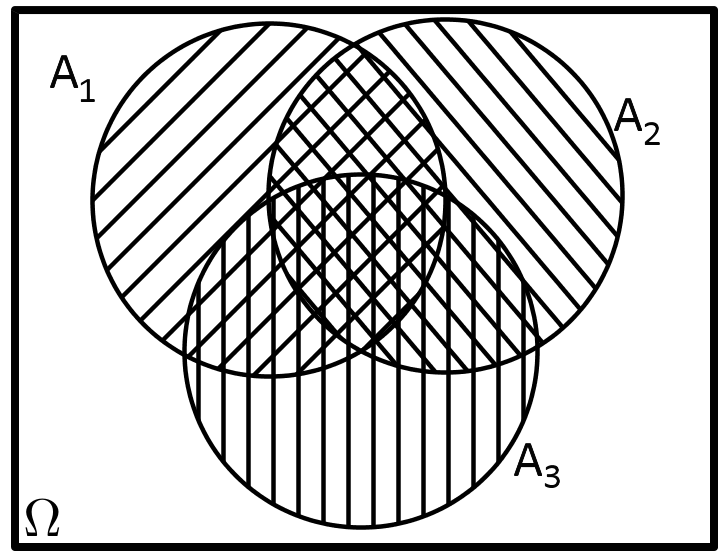
\includegraphics[height=5.5cm]{../fig/Cap03-DiagramaVennUnioTresSucesos.png}
	\caption{Diagrama para la intersección de tres sucesos.}
    \label{Cap03:fig:DiagramaVennUnioTresSucesos}
\end{center}
\end{figure}




\section{Probabilidad condicionada. Sucesos independientes.}
\label{cap03:sec:ProbabilidadCondicionadaIndependencia}


\subsection{Probabilidad condicionada.}
\label{cap03:subsec:ProbabilidadCondicionada}

El concepto de probabilidad condicionada trata de reflejar los cambios en el
valor de la Función Probabilidad que se producen cuando tenemos {\em
información parcial} sobre el resultado de un experimento aleatorio. Para
entenderlo, vamos a usar, como ejemplo, uno de esos casos en los que la Regla
de Laplace es suficiente para calcular probabilidades. Vamos a pensar que, al
lanzar dos dados, nos dicen que la suma de los dados ha sido mayor que 3.
Pero imagina que no sabemos el resultado; puede ser $(1,3), (2,5)$, etc.,
pero no, por ejemplo, $(1,1)$, o $(1,2)$. Con esa información en nuestras
manos, nos piden que calculemos la probabilidad de que la suma de los dos
dados haya sido un $7$. Nuestro cálculo debe ser distinto ahora que sabemos
que el resultado es mayor que 3, porque el número de resultados posibles (el
denominador en la fórmula de Laplace), ha cambiado. Los resultados como
$(1,1)$ o $(2,1)$ no pueden estar en la lista de resultados posibles, {\em si
sabemos que la suma es mayor que $3$}.  {\sf\em La información que tenemos
sobre el resultado cambia nuestra asignación de probabilidades}. Este es un
buen momento para recordar el problema de Monty Hall (y volver a recomendar
al lector que, si no lo hizo, busque el vídeo de la serie Numb3rs del que ya
hemos hablado).

Usando como ``laboratorio de ideas'' la Regla de Laplace, estamos tratando de
definir la {\em probabilidad del suceso $A$, {\sf sabiendo} que ha ocurrido
el suceso $B$}. Esto es lo que vamos a llamar la \index{probabilidad
condicionada} {\sf probabilidad de $A$ condicionada por $B$, y lo
representamos por $P(A|B)$}. Pensemos en cuáles son los cambios en la
aplicación de la Regla de Laplace (favorables/posibles), cuando sabemos que
el suceso $B$ ha ocurrido. Antes que nada recordemos que, si el total de
resultados elementales posibles es $n$ entonces
    \[P(A)=\dfrac{\mbox{núm. de casos favorables a $A$}}{n},\]
y también se cumple
    \[P(B)=\dfrac{\mbox{núm. de casos favorables a $B$}}{n}.\]
Veamos ahora como deberíamos definir $P(A|B)$. Puesto que sabemos que $B$ ha
ocurrido, los casos posibles ya no son todos los $n$ casos posibles
originales: ahora los únicos casos posibles son los que corresponden al
suceso $B$.  ¿Y cuáles son los casos favorables del suceso $A$, una vez que
sabemos que $B$ ha ocurrido? Pues aquellos casos en los que $A$ y $B$ ocurren
simultáneamente (o sea, el suceso $A\cap B$). En una fracción:
    \[P(A|B)=\dfrac{\mbox{número de casos favorables a $A\cap B$}}{\mbox{número de casos favorables a $B$}}.\]
Si sólo estuviéramos interesados en la Regla de Laplace esto sería tal vez
suficiente. Pero, para poder generalizar la fórmula a otras situaciones, como
la Probabilidad Geométrica, hay una manera mejor de escribirlo. Dividimos el
numerador y el denominador por $n$ y tenemos:
    \[P(A|B)=\dfrac{\quad\left(\dfrac{\mbox{número de casos favorables a $A\cap B$}}{n}\right)\quad}{\left(\dfrac{\mbox{número de casos favorables a $B$}}{n}\right)}=\dfrac{P(A\cap B)}{P(B)}.\]
¿Qué tiene de bueno esto? Pues que la expresión que hemos obtenido ya no hace
ninguna referencia a casos favorables o posibles, nos hemos librado de la
Regla de Laplace, y hemos obtenido una expresión general que sólo usa la
Función de Probabilidad (e, insistimos, hacemos esto porque así podremos
usarla, por ejemplo, en problemas de Probabilidad Geométrica). Ya tenemos la
definición:
    \begin{center}
    \fcolorbox{black}{Gris025}{
    \begin{minipage}{12cm}
        {\centering {\bf Probabilidad condicionada:}}\\
        \label{cap03:def:ProbabilidadCondicionada}
        La probabilidad del suceso $A$ condicionada por el suceso $B$ se define así:
        \[P(A|B)=\dfrac{P(A\cap B)}{P(B)}.\]
        donde se supone que $P(B)\neq 0$.
    \end{minipage}}
    \end{center}
%
%
%
%
%
%        \begin{center}
%        \fbox{\colorbox{Gris025}{\begin{minipage}{14cm}
%        \begin{center}
%%        \vspace{2mm}
%        {\bf Probabilidad condicionada: }
%        \end{center}
%        La probabilidad del suceso $A$ condicionada por el suceso $B$ se define así:
%            \[P(A|B)=\dfrac{P(A\cap B)}{P(B)}.\]
%        donde se supone que $P(B)\neq 0$.
%        \end{minipage}}}
%        \end{center}

Vamos a ver un ejemplo de como calcular estas probabilidades condicionadas, usando de nuevo el lanzamiento de dos dados.
    \begin{Ejemplo}
    \label{Cap03:probabilidadCondicionadaLanzamientoDosDados}
    Se lanzan dos dados. ¿Cuál es la probabilidad de que la diferencia (en valor absoluto) entre los valores de ambos dados (mayor-menor) sea menor que 4, sabiendo que la suma de los dados es 7?\\
    Vamos a considerar los sucesos:
    \begin{itemize}
        \item[S:] La suma de los dados es 7.
        \item[D:] La diferencia en valor absoluto de los dados es menor que 4.
    \end{itemize}
    En este caso es muy fácil calcular $P(D|S)$. Si sabemos que la suma es $7$, los resultados sólo pueden ser $(1,6),(2,5),(3,4),(4,3),(5,2),(6,1)$. Y de estos, sólo $(1,6)$ y $(6,1)$ no cumplen la condición de la diferencia. Así que $P(D|S)=4/6$. Vamos a ver si coincide con lo que predice la fórmula. El suceso $S\cap D$ ocurre cuando ocurren {\sf a la vez} $S$ y $D$. Es decir la suma es 7 {\sf y a la vez} la diferencia es menor que $4$. Es fácil ver que, de los 36 resultados posible, eso sucede en estos cuatro casos: \[(2,5),(3,4),(4,3),(5,2),\]
    por tanto, la probabilidad de la intersección es $P(S\cap D)=\frac{4}{36}$. Y, por otro lado, la probabilidad del suceso $S$ es $P(S)=\frac{6}{36}$ (ver el Ejemplo \ref{Cap03:ejem:CualEsProbabilidadSumaDosDadosIgualASiete} de la pág. \pageref{Cap03:ejem:CualEsProbabilidadSumaDosDadosIgualASiete}; de hecho, hemos descrito los sucesos favorables a $S$ un poco más arriba). Así pues,
    \[P(D|S)=\dfrac{P(D\cap S)}{P(S)}=\dfrac{4/36}{6/36}=\dfrac{4}{6}=\dfrac{2}{3}\approx 0.666\ldots,\]
    como esperábamos. En el Tutorial3 veremos como usar el ordenador para simular este experimento, y comprobar los resultados que predice la teoría.
    \qed
    \end{Ejemplo}
En realidad, la probabilidad condicionada se usa habitualmente para calcular
la probabilidad de una intersección. Este método se basa en la siguiente
reformulación de la definición, llamada {\sf Regla del Producto} para las
probabilidades condicionadas.
        \begin{center}
        \fcolorbox{black}{Gris025}{
        \begin{minipage}{8cm}
        \begin{equation}\label{cap03:ecu:ReglaProductoProbabilidadCondicionada}
            P(A|B)P(B)=P(B|A)P(A),
        \end{equation}
        \end{minipage}}
        \end{center}
porque la definición de probabilidad condicionada dice que los dos miembros son dos formas de escribir $P(A\cap B)$. Teniendo esto en cuenta, si se conocen las probabilidades de $A$ y $B$, se puede obtener fácilmente una probabilidad condicionada a partir de la otra. Este resultado es extremadamente útil para, por ejemplo, descomponer problemas de probabilidad en varias etapas, y usar las probabilidades condicionadas, normalmente más fáciles de calcular.

\subsubsection{Tablas de contingencia y probabilidad condicionada}
\label{cap03:subsubsec:TablasContingenciaProbabilidadCondicionada}

    La noción de probabilidad condicionada $P(A|B)$ se utiliza a menudo en situaciones en las que la información sobre los sucesos $A$ y $B$ (y sus complementarios $A^c$ y $B^c$) se presenta en forma de tablas, que en este contexto se llaman {\sf tablas de contingencia}\index{tabla de contingencia}. Las tablas de contingencia aparecerán varias veces en el curso, y en el Capítulo \ref{cap:TablasContingenciaTestChi2} hablaremos extensamente sobre ellas. En el próximo ejemplo vamos a ver un caso típico, y clásico, de aplicación del concepto de probabilidad condicionada: las {\sf pruebas diagnósticas}\index{pruebas diagnósticas}\index{diagnósticas, pruebas}, para la detección de una enfermedad.
\begin{ejemplo}
\label{cap03:ejem:PruebasDiagnosticas01}
\index{pruebas diagnósticas}\index{diagnósticas, pruebas}
           Vamos a suponer que analizamos una prueba diagnóstica para cierta enfermedad. Las pruebas diagnósticas no son infalibles. A veces la prueba dará como resultado que una persona padece la enfermedad, cuando en realidad no es así. Es lo que se llama un {\sf falso positivo}\index{falso positivo}. Y en otras ocasiones el problema será el contrario. La prueba dirá que la persona no padece la enfermedad, aunque de hecho la padezca. Eso es un {\sf falso negativo}\index{falso negativo}. Vamos a suponer que sabemos en una población de 10000, aproximadamente, el 2\% están afectados por esa enfermedad. La Tabla \ref{cap03:tabla:ejemploPruebasDiagnosticas}, que es típica de esta clase de situaciones, contiene los valores precisos de este ejemplo.
        \begin{table}[h!]
        \begin{center}
            \begin{tabular}{llccc}
            &&\multicolumn{3}{c}{\underline{\bf Padecen la enfermedad}}\\

                                      &          & Sí &  No & Total\\
            \hline
          \underline{\bf Resultado de la Prueba} & Positivo & 192&  158&   350\\
                                      & Negativo &  4 & 9646&  9650\\
            \hline
                                      & Total    & 196& 9804& 10000\\
            \hline
            \end{tabular}
        \end{center}
        \caption{Tabla de contingencia del Ejemplo \ref{cap03:ejem:PruebasDiagnosticas01}}
        \label{cap03:tabla:ejemploPruebasDiagnosticas}
        \end{table}

        Como puede verse en esa tabla, hay dos {\em familias de sucesos} en las que podemos pensar:
        \begin{itemize}
           \item sano o enfermo.
           \item resultado positivo o negativo de la prueba diagnóstica.
         \end{itemize}
        Estas dos familias de sucesos representan dos formas de dividir o clasificar a la población (en sanos/enfermos por un lado, o en positivos/negativos por otro lado).

        Para calcular la probabilidad de que un individuo esté sano, debemos mirar en el {\em margen inferior} (de otro modo, la última fila de la tabla). Allí vemos que hay 196 personas enfermas de un total de 10000. Por lo tanto, la probabilidad es:
        \[P(\mbox{enfermo})=\dfrac{196}{10000}=0.0196.\]
        Como decíamos antes, aproximadamente un 2\%. Puesto que, en este ejemplo, suponemos que una persona sólo puede estar sana o enferma, la probabilidad de enfermo es:
        \[P(\mbox{sano})=1-P(\mbox{enfermo})=1-0.0196=0.9804.\]
        Este resultado también se puede obtener, directamente, del margen inferior de la tabla. Si en lugar de sano/enfermo pensamos en las probabilidades de diagnóstico positivo/negativo, entonces tenemos que mirar en el {\em margen derecho} (la última columna) de la tabla. Allí vemos que, de las 10000 personas, 350 han dado positivo, así que
        \[P(\mbox{positivo})=\dfrac{350}{10000}=0.035.\]
        De la misma forma (o restando de uno) se tiene:
        \[P(\mbox{negativo})=\dfrac{9650}{10000}=0.965.\]
        Con esto vemos que los márgenes de la tabla (inferior y derecho) nos permiten obtener las probabilidades de las dos familias de sucesos que intervienen en este ejemplo. ¿Qué significado tienen, en términos de probabilidades, los cuatro valores {\em interiores de la tabla} (los que ocupan las dos primeras filas y columnas)? Por ejemplo, ¿qué representa el valor 4 de la segunda fila, primera columna? Se trata del número de personas que, a la vez, padecen la enfermedad y han dado negativo en el diagnóstico. Por lo tanto ese número se refiere al suceso intersección
        \[\mbox{enfermo}\cap\mbox{negativo},\]
        y su probabilidad es:
        \[P\left(\mbox{enfermo}\cap\mbox{negativo}\right)=\dfrac{4}{10000}=0.0004\]
        De la misma forma, para los otro tres valores:
        \[
        \begin{cases}
        P\left(\mbox{enfermo}\cap\mbox{positivo}\right)=\dfrac{192}{10000}=0.0192\\[5mm]
        P\left(\mbox{sano}\cap\mbox{positivo}\right)=\dfrac{158}{10000}=0.0158\\[5mm]
        P\left(\mbox{sano}\cap\mbox{negativo}\right)=\dfrac{9646}{10000}=0.9646
        \end{cases}
        \]
        ¿Y las probabilidades condicionadas? Esas probabilidades no se ven directamente en una tabla como la Tabla \ref{cap03:tabla:ejemploPruebasDiagnosticas}. Pero podemos obtenerlas fácilmente, operando por filas o por columnas, según se trate. Por ejemplo, para calcular
        \[P\left(\mbox{negativo} | \mbox{enfermo} \right),\]
        puesto que sabemos que el individuo está enfermo, tenemos que limitarnos a considerar los $196$ individuos de la primera columna. De esos, la segunda fila nos informa de que sólo $4$ han dado negativo en la prueba, lo cual significa que:
        \[P\left(\mbox{negativo} | \mbox{enfermo} \right)=\dfrac{4}{196}\approx 0.02.\]
        Es decir, que hay sólo un 2\% de falsos negativos. De la misma forma:
        \[P\left(\mbox{positivo} | \mbox{sano} \right)=\dfrac{158}{9804}\approx 0.016,\]
        demuestra que la prueba tiene también una tasa muy baja de falsos positivos. Estos dos resultados nos hacen pensar que la prueba diagnóstica es muy buena, así que cuando un paciente recibe un diagnóstico positivo, lo normal es que piense que hay una probabilidad muy alta de estar enfermo. Pero ¿cuál es, realmente, esa probabilidad? Tenemos que calcular
        \[P\left(\mbox{enfermo} | \mbox{positivo}\right),\]
        y ahora, puesto que sabemos que el individuo ha dado positivo, tenemos que limitarnos a considerar los $350$ individuos de la primera fila. De esos, la primera columna nos dice que $192$ están, de hecho enfermos. Así que la probabilidad que buscamos es:
        \[P\left(\mbox{enfermo} | \mbox{positivo}\right)=\dfrac{192}{350}\approx 0.5486.\]
        Apenas un 55\%. ¿Cómo es posible, si la prueba parecía ser tan buena? La explicación, y es esencial mirar atentamente la Tabla \ref{cap03:tabla:ejemploPruebasDiagnosticas} para entenderla, es que realmente hay muy pocas personas enfermas, sobre el total de la población. Así que los falsos positivos, que se calculan sobre una gran cantidad de personas sanas, representan una fracción muy importante del total de positivos.
        \qed
      \end{ejemplo}
      Después de ver este ejemplo,  puede ser un buen momento para que el lector, si no la conoce, escuche la charla TED de Peter Donnelly (ver el enlace [\,\ref{enlace0007}\,]\label{enlace0007a}), titulada {\em ``How juries are fooled by statistics''} (``La Estadística engaña a los jurados''; hay subtítulos en español o inglés). La charla trata sobre Probabilidad, Estadística, y el papel que juegan en terrenos tan variados como la Genética, o los procesos judiciales.

      La Tabla \ref{cap03:tabla:ejemploPruebasDiagnosticas} es, como hemos dicho, un ejemplo de una {\sf tabla de contingencia}. En este caso es una tabla $2\times 2$, pero veremos más adelante (en el Capítulo \ref{cap:TablasContingenciaTestChi2}) otros ejemplos en los que se hace necesario contemplar tablas de contingencia de dimensiones distintas.


\subsection{Sucesos independientes.}
\label{cap03:subsec:SucesosIndependientes}

¿Qué significado debería tener la frase {\em ``el suceso $A$ es independiente del suceso $B$''}\,? Parece evidente que, si los sucesos son independientes, el hecho de saber que el suceso $B$ ha ocurrido no debería afectar para nada nuestro cálculo de la probabilidad de que ocurra $A$. Esta idea tiene una traducción inmediata en el lenguaje de la probabilidad condicionada, que es de hecho la definición de sucesos independientes:
        \begin{center}
        \fcolorbox{black}{Gris025}{
        \begin{minipage}{12cm}
            {\centering\bf Sucesos independientes}
            Los sucesos $A$ y $B$ son \index{sucesos independientes}{\sf sucesos independientes}\index{independientes, sucesos} si
                \[P(A|B)=P(A).\]
            Esto es equivalente a decir que:
            \begin{equation}\label{cap03:ecu:ReglaProductoProbabilidadDosSucesosIndependientes}
                P(A\cap B)=P(A)P(B).
            \end{equation}
            Esta propiedad se conoce como la {\sf Regla del Producto para sucesos independientes.}\index{regla del producto para sucesos independientes}\index{sucesos independientes, regla del producto}\\
            En particular, {\bf cuando los sucesos $A$ y $B$ son independientes}, se cumple:
            \[P(A\cup B)=P(A)+P(B)-P(A)P(B).\]
        \end{minipage}}
        \end{center}
En general los sucesos $A_1,\ldots,A_k$ son independientes cuando para {\em cualquier colección} que tomemos de ellos, la probabilidad de la intersección es el producto de las probabilidades. Eso significa que, en particular, sucede
    \begin{equation}\label{cap03:ecu:ReglaProductoProbabilidad_N_SucesosIndependientes}
        P(A_1\cap A_2\cap\cdots\cap A_k)=P(A_1) \cdot P(A_2)\cdot\cdots\cdot P(A_k).\mbox{ {!`}{!`}Para sucesos independientes!!}
    \end{equation}
Pero insistimos, la independencia significa que esto debe cumplirse para cualquier subcolección. Por ejemplo,  para que $A_1,\ldots,A_5$ sean independientes, debe cumplirse
\[P(A_1\cap A_2\cap A_4)=P(A_1)\cdot P(A_2)\cdot P(A_4),\]
pero también
\[P(A_1\cap A_5)=P(A_1)\cdot P(A_5),\]
entre otras muchas. ¿Cuántas? Es un buen ejercicio de Combinatoria convencerse de que son $2^k - k -1$, donde $k$ es el número de sucesos. {!`}Verificar la independencia de una colección de sucesos puede ser muy complicado! Normalmente partiremos de situaciones en las que sabemos {\em a priori} que se cumple la independencias, y entonces usaremos estas propiedades para poder calcular las probabilidades de las intersecciones que nos interesen.

\subsubsection{Sucesos independientes y sucesos disjuntos (incompatibles)}

A menudo, al principio, hay cierta confusión entre la noción de sucesos independientes y la de sucesos disjuntos, que también hemos llamado incompatibles. Tal vez sea el origen de la confusión tenga algo que ver con el parecido entre esas dos palabras.  En cualquier caso, recordemos que dos sucesos son disjuntos si no pueden ocurrir a la vez (ver Figura \ref{Cap03:fig:DiagramaVennSucesosDisjuntos}, pág. \pageref{Cap03:fig:DiagramaVennSucesosDisjuntos}). Por ejemplo, si $A$ es el suceso {\em ``Hoy es lunes''} y $B$ es el suceso {\em ``Hoy es viernes''}, está
claro que $A$ y $B$ no pueden ocurrir a la vez. Por otra parte, los sucesos son independientes cuando uno de ellos no aporta ninguna información sobre
el otro. Y volviendo al ejemplo, en cuanto sabemos que hoy es lunes (ha ocurrido $A$), ya estamos seguros de que no es viernes (no ha ocurrido $B$).
Así que la información sobre el suceso $A$ nos permite decir algo sobre el suceso $B$, y eso significa que no hay independencia.
        \begin{center}
        \fcolorbox{black}{Gris025}{
        \begin{minipage}{8cm}
                        {\sf Dos sucesos disjuntos nunca son independientes.}
        \end{minipage}}
        \end{center}

\section{Probabilidades totales y Teorema de Bayes.}
\label{cap03:sec:ProbabilidadesTotalesReglaBayes}


\subsection{La regla de las probabilidades totales. Problemas de urnas.}
\label{cap03:subsec:ProbabilidadesTotales}


El resultado que vamos a ver utiliza la noción de probabilidad condicionada para calcular la probabilidad de un suceso $A$ mediante la estrategia de {\em divide y vencerás}.  Se trata de descomponer el espacio muestral completo en una serie de sucesos $B_1,\ldots,B_k$ de manera que:
    \begin{enumerate}
        \item[(1)] $\Omega=B_1\cup B_2\cup\cdots\cup B_k.$
        %\textcolor{red}{Es decir, cada evento elemental est\'an en alguno de los $B_i$.}
        \item[(2)] $B_i\cap B_j=\emptyset$, para cualquier pareja $i\neq j$:
        %\textcolor{red}{ning\'un evento evento elemental est\'a repetido.}
        \item[(3)] $P(B_i)\neq 0$ para $i=1,\ldots,k$.
        %\textcolor{red}{Todos los eventos $B_i$ son posibles.}
    \end{enumerate}
{En este caso se dice que los sucesos $B_1,\ldots,B_k$ constituyen una partici\'on (1)
disjunta (2) del espacio muestral. \index{partici\'on disjunta del espacio muestral}} Entonces
        \begin{center}
        \fcolorbox{black}{Gris025}{
        \begin{minipage}{12cm}
            {\centering\bf Regla de las probabilidades totales\index{regla de las probabilidades totales}}
            Si los sucesos $B_1,\ldots,B_K$ cumplen las condiciones (1), (2) y (3) entonces:
            \[P(A)=P(B_1)P(A|B_1)+P(B_2)P(A|B_2)+\cdots+P(B_k)P(A|B_k).\]
        \end{minipage}}
        \end{center}
Esta expresión permite calcular la probabilidad de $A$ cuando conocemos de antemano las probabilidades de los sucesos $B_1,\ldots,B_k$ y es fácil calcular las probabilidades condicionadas $P(A|B_i)$. Si los sucesos $B_i$ se han elegido bien, la información de que el suceso $B_i$ ha ocurrido puede en ocasiones simplificar mucho el cálculo de $P(A|B_i)$.

El método de las probabilidades totales se usa sobre todo cuando conocemos varias vías o mecanismos por los que el suceso $A$ puede llegar a producirse. El ejemplo clásico son los {\sf problemas de urnas}, que sirven de prototipo para muchas otras situaciones.
    \begin{Ejemplo}
    \label{cap03:ejem:ProbailidadTotalEjemploUrnas}
        Supongamos que tenemos dos urnas, la primera con 3 bolas blancas y dos negras, y la segunda con 4 bolas blancas y 1 negra. Para extraer una bola lanzamos un dado. Si el resultado es $1$ o $2$ usamos la primera urna; si es cualquier otro número usamos la segunda urna. ¿cuál es la probabilidad de obtener una bola blanca?\\
        Llamemos $A$ al suceso {\em ``ha salido una bola blanca''} ,  $B_1$ al suceso {\em ``se ha usado la primera urna''}, y $B_2$ al suceso {\em ``se ha usado la segunda urna''}. Entonces,de la regla de Laplace obtenemos $P(B_1)=\frac{1}{3}$, $P(B_2)=\frac{2}{3}$. Y ahora, cuando sabemos que $B_1$ ha ocurrido (es decir, que estamos usando la primera urna), es fácil calcular $P(A|B_1)$.  Se trata de la probabilidad de extraer una bola blanca de la primera urna: $P(A|B_1)=\frac{3}{5}.$ De la misma forma $P(A|B_2)=\frac{4}{5}$. Con todos estos datos, el Teorema de las Probabilidades Totales da como resultado:
        \[P(A)=P(B_1)P(A|B_1)+P(B_2)P(A|B_2)=
        \dfrac{1}{3}\cdot\dfrac{3}{5}+\dfrac{2}{3}\cdot\dfrac{4}{5}=\dfrac{11}{15}.\]
        En el Tutorial-03 usaremos el ordenador para verificar, mediante una simulación, estos resultados.
    \qed
    \end{Ejemplo}
Este ejemplo, con dados y bolas, puede parecer artificioso, y alejado de las aplicaciones prácticas. Pero piensa en esta situación: si tenemos una fábrica que produce la misma pieza con dos máquinas distintas, y sabemos la proporción de piezas defectuosas que produce cada una de las máquinas, podemos identificar máquinas con urnas y piezas con bolas, y vemos que el método de las probabilidades totales nos permite saber cuál es la probabilidad de que una pieza producida en esa fábrica sea defectuosa. De la misma forma, si sabemos la probabilidad de desarrollar cáncer de pulmón, en  fumadores y no fumadores, y sabemos la proporción de fumadores y no fumadores que hay en la población total, podemos identificar cada uno de esos tipos de individuos (fumadores y no fumadores) con una urna, y el hecho de desarrollar o no cáncer con bola blanca o bola negra. Como puede verse, el rango de aplicaciones de este resultado es bastante mayor de lo que parecía a primera vista.


\subsection{Teorema de Bayes. La probabilidad de las causas.}
\label{cap03:subsec:TeoremaBayesProbabilidadCausas}



La regla de las probabilidades totales puede describirse así: si conocemos varios mecanismos posibles (los sucesos $B_1,\ldots,B_k$) que dan como resultado el suceso $A$, y las probabilidades asociadas con esos mecanismos, ¿cuál es la probabilidad de ocurra el suceso $A$? El Teorema de Bayes le da la vuelta a la situación. Ahora suponemos que el suceso $A$ {\em de hecho ha ocurrido}.  Y, puesto que puede haber ocurrido a través de distintos mecanismos, nos podemos preguntar ¿cómo de probable es que el suceso $A$ haya ocurrido a través de, por ejemplo, el primer mecanismo $B_1$? Insistimos, no vamos a preguntarnos por la probabilidad del suceso $A$, puesto que suponemos que ha ocurrido. Nos preguntamos por la probabilidad de cada una de los mecanismos o causas que conducen al resultado $A$. Por eso a veces el Teorema de Bayes se describe como un resultado sobre la probabilidad de las causas.

¿Cómo podemos conseguir esto? La pregunta se puede formular así: sabiendo que el suceso $A$ ha ocurrido, ¿cuál es la probabilidad de que haya ocurrido a través del mecanismo $B_i$? De otra manera: sabiendo que el suceso $A$ ha ocurrido, ¿cuál es la probabilidad de que eso se deba a que $B_i$ ha ocurrido? Es decir, queremos averiguar el valor de
    \[P(B_i|A)\mbox{\quad para i=1,\ldots,k}.\]
Quizá lo más importante es entender que, para calcular este valor, {\em la información de la que disponemos es exactamente la misma que en el caso de las probabilidades totales}. Es decir, conocemos los valores $P(B_1),\ldots,P(B_k)$ y las probabilidades condicionadas $P(A|B_1),\ldots,P(A|B_k)$, {!`}qué son justo al revés de lo que ahora queremos!.

Y la forma de conseguir el resultado es esta. Usando que:
    \[P(A|B_k)P(B_k)=P(A\cap B_k)=\colorbox{lightgrey}{$P(B_k|A)$}P(A),\]
despejamos de aquí lo que queremos, y usamos el teorema de las probabilidades totales de una forma astuta, obteniendo:
\begin{center}
    \fcolorbox{black}{Gris025}{
    \begin{minipage}{13cm}
        {\centering\bf Teorema de Bayes\index{teorema de Bayes}}
        Si los sucesos $B_1,\ldots,B_k$ cumplen las condiciones (1), (2) y (3) (ver la Sección \ref{cap03:subsec:ProbabilidadesTotales}), entonces para cualquier $j$ de $1$ a $k$ se tiene:
        {\small
        \[P(B_j|A)=\dfrac{P(B_k)P(A|B_k)}{P(A)} = \dfrac{P(B_k)P(A|B_k)}{P(B_1)P(A|B_1)+P(B_2)P(A|B_2)+\cdots+P(B_k)P(A|B_k)}.\]
        }
    \end{minipage}}
    \end{center}
Obsérvese que:
    \begin{enumerate}
    \item Los valores que necesitamos para calcular esta fracción aparecen en la fórmula de las probabilidades totales.
    \item El numerador es uno de los sumandos del denominador.
    \item Las probabilidades condicionadas de la fracción son justo al revés que las del miembro izquierdo.
    \item El denominador es la probabilidad $P(A)$, calculada a través del teorema de las probabilidades totales.
    \end{enumerate}
Con estas observaciones, la fórmula de Bayes es bastante fácil de recordar. Vamos a ver dos ejemplos de este teorema, ambos relacionados con ejemplos anteriores de este capítulo.
El primero es el ejemplo prototípico, un problema de urnas, que sólo tiene el interés de que nos sirve como modelo mental de la forma en que se aplica el teorema.
\begin{Ejemplo}
    {\bf Continuación del Ejemplo \ref{cap03:ejem:ProbailidadTotalEjemploUrnas}, pág. \pageref{cap03:ejem:ProbailidadTotalEjemploUrnas}}\label{cap03:ejem:EjemploUrnasBayes}
    Recordemos que, en aquel ejemplo, teníamos dos urnas. La primera con 3 bolas blancas y dos negras, y la segunda con 4 bolas blancas y 1 negra. Para extraer una bola, se lanza un dado. Si el resultado es $1$ o $2$ usamos la primera urna; si es cualquier otro número usamos la segunda urna.
    Supongamos que hemos hecho ese proceso, y la bola extraída es blanca. ¿Cuál es la probabilidad de que proceda de la primera urna?

    Según nuestra experiencia, los ejercicios del Teorema de Bayes se encuentran entre los que más dificultades causan a los novatos, en cursos como este. Así que vamos a tomarnos este ejemplo con calma, y vamos a detallar minuciosamente, paso a paso, cómo lo abordamos.

    Cuando nos enfrentamos a un problema como este, es crucial aprender a procesar la información del enunciado de forma adecuada. En primer lugar, hay que reconocer una situación como la que hemos descrito, con dos familias {\em básicas} $A$ y $B$ de fenómenos (no importa cuál es $A$ y cuál es $B$). En este ejemplo:
    \begin{enumerate}
    \item Familia $A$: $A_1$ es ``bola blanca'' y $A_2$ es ``bola negra''.
    \item Familia $B$: $B_1$ es ``urna 1'' y $B_2$ es ``urna 2''. (Es lo mismo que $B_1$ es ``dado de dos para abajo'' y $B_2$ es ``dado de tres para arriba'').
    \end{enumerate}
    Un par de observaciones sobre esta notación: en el Ejemplo \ref{cap03:ejem:ProbailidadTotalEjemploUrnas} no hemos distinguido entre suceso $A_1$ y suceso $A_2$. En parte porque se nos preguntaba directamente por una bola blanca, y en parte porque la pregunta era más sencilla. Pero aquí nos conviene ser muy cuidadosos con la notación. Y también es cierto que podríamos decir que $A$ es ``bola blanca'', y $A^c$ es ``bola negra''. Pero nos encontraremos más adelante con muchos ejemplos de problemas de Bayes que son, por así decirlo, multicolores. Cuando encontremos un problema con bolas blancas, negras, rojas, azules, etc., no tendremos más remedio que usar $A_1, A_2, A_3,\ldots$

    Insistimos en que, en este primer paso, las dos familias de sucesos deben ser básicas, en el sentido de muy sencillas de describir. Uno de los errores más comunes que vemos cometer a los principiantes, es elegir un suceso como:
    ``Sale una bola blanca de la urna 1''
    y llamarlo $A_1$. Hay que evitar estas mezclas de ``urnas con bolas'', si no queremos perdernos por el camino.

    Cuando tenemos claro cuáles son las dos familias de sucesos $A$ y $B$ que vamos a usar, podemos empezar a traducir la información del enunciado a probabilidades. Hay que estar atentos, porque en un ejercicio del Teorema de Bayes, {\sf siempre} suceden estas tres cosas:
    \begin{enumerate}
        \item Se nos pide que calculemos una probabilidad condicionada. A menudo lo más fácil es empezar por lo que suele ser el final del enunciado, la pregunta. Y a partir de ahí, una vez entendido lo que nos preguntan, y traducido a probabilidades, volver hacia atrás y ver cuál es la información que nos han dado en el enunciado.\\
            En este ejemplo la pregunta dice ``...hemos hecho ese proceso, y la bola extraída es blanca. ¿Cuál es la probabilidad de que proceda de la primera urna?'' Recordamos que nos preguntan por una probabilidad condicionada, y vemos que es la probabilidad de que se haya usado la urna 1. Así que ya sabemos que, con la elección de nombres que hemos hecho antes, la pregunta es de la forma:
            \[P(B_1\,|\,?\,).\]
            ¿Cuál es el suceso que condiciona? Es decir, ¿cuál es el que debe aparecer a la derecha de la barra en esta probabilidad condicionada? Para saberlo, tenemos que recordar que esa probabilidad condicionada se puede leer ``probabilidad de $B_1$ sabiendo que ha sucedido...''. Y ahora, volvemos a la pregunta buscando algo que el enunciado {\sf nos garantiza que ha sucedido}. La clave es el principio de la frase ``...hemos hecho ese proceso, y la bola extraída es blanca.'' Este enunciado asegura que, de hecho, ha ocurrido el suceso $A_1$ ``la bola es blanca''. Así que lo pide este ejercicio es que calculemos
            \[P(B_1 | A_1).\]
        \item Muchas personas, tras localizar lo que pide el enunciado, escriben directamente la fórmula de Bayes que se necesita. Que, en este ejemplo sería:
            \[P(B_1 | A_1)=\dfrac{P(A_1 | B_1)\cdot P(B_1)}{P(A_1 | B_1)\cdot P(B_1)+P(A_1 | B_2)\cdot P(B_2)}.\]
            Nosotros invitamos al lector a que, sobre todo hasta que haya ganado en experiencia, tenga un poco de paciencia, y que analice y reúna la información que ofrece el resultado, {\sf antes} de escribir la fórmula. Es una cuestión puramente táctica: cuando tenemos la fórmula delante, la tentación de encajar los valores del enunciado en los ``huecos'' que ofrece la fórmula, a menudo nos hace precipitarnos y cometer errores. La habilidad con los ejercicios del Teorema de Bayes se adquiere mediante la familiaridad  con la fórmula, y una buena dosis de experencia interpretando enunciados.

        \item El enunciado contiene información sobre probabilidades condicionadas, del tipo contrario a la que debemos calcular.\\
            En este ejemplo, puesto que tenemos que calcular $P(B_1 | A_1)$, el enunciado nos dará información sobre probabilidades de la forma $P(A_i|B_j)$. Concretamente, esas probabilidades son ``probabilidad de que la bola sea de tal color, sabiendo que procede de tal urna''.  Son justo el tipo de probabilidades que calculábamos en el Ejemplo \ref{cap03:ejem:ProbailidadTotalEjemploUrnas}. Y tenemos esa misma información, así que podemos calcular cualquiera de las probabilidades $P(A_1|B_1)$, $P(A_1|B_2)$, $P(A_2|B_1)$ o $P(A_2|B_2)$. Necesitaremos concretamente $P(A_1 | B_1)$ y $P(A_1 | B_2)$ (aparecen en el numerador de la fórmula de Bayes), que, usando la composición de las urnas, son:
            \[
            \begin{cases}
                P(A_1 | B_1)=\dfrac{3}{5}& \mbox{(bola blanca, urna 1)}.\\[5mm]
                P(A_1 | B_2)=\dfrac{4}{5}& \mbox{(bola blanca, urna 2)}.
            \end{cases}
            \]

        \item Además, el enunciado siempre contiene información sobre probabilidades no condicionadas. De hecho, puesto que tenemos que calcular $P(B_1|A_1)$, el enunciado nos dará probabilidad sobre sucesos de la familia $B$ (la que aparezca a la izquierda de la barra vertical).\\
            En este ejemplo, los sucesos $B_1$ y $B_2$ identifican cuál es la urna que se ha usado. Y eso se determina, como explica el enunciado, lanzando un dado y viendo si el resultado es 1 o 2 (urna 1), o si es alguno de los restantes números (urna 2). Así que, teniendo en cuenta las instrucciones del enunciado, tenemos:
            \[P(B_1)=\dfrac{2}{6}, \quad P(B_2)=\dfrac{4}{6}.\]

    \end{enumerate}
    Con estos tres ingredientes, ya estamos listos para completar la cuenta. Sustituimos los valores necesarios en la fórmula:
            \[P(B_1 | A_1)=\dfrac{P(A_1 | B_1)\cdot P(B_1)}{P(A_1 | B_1)\cdot P(B_1)+P(A_1 | B_2)\cdot P(B_2)}=\dfrac{\dfrac{3}{5}\cdot \dfrac{2}{6}}{\dfrac{3}{5}\cdot \dfrac{2}{6}+\dfrac{4}{5}\cdot\dfrac{4}{6}}=\dfrac{3}{11}.\]
    Proponemos al lector, como ejercicio (que ahora debería ser fácil), que calcule la probabilidad de que la bola proceda de la urna 2, sabiendo que ha resultado ser negra. \qed
\end{Ejemplo}

En el siguiente ejemplo vamos a aplicar las mismas técnicas de análisis del enunciado al caso de las pruebas diagnósticas, en las que el Teorema de Bayes juega un papel especialmente importante.
\begin{ejemplo}
\label{cap03:ejem:PruebasDiagnosticasBayes}
    \index{pruebas diagnósticas}\index{diagnósticas, pruebas}
    Vamos a utilizar los mismos datos que en el Ejemplo \ref{cap03:ejem:PruebasDiagnosticas01}, en el que teníamos toda la información en forma de tabla de contingencia, (ver la Tabla \ref{cap03:tabla:ejemploPruebasDiagnosticas}, pág. \pageref{cap03:tabla:ejemploPruebasDiagnosticas}). En aquel ejemplo calculábamos, a partir de la Tabla, varias probabilidades condicionadas. Concretamente, obtuvimos:
    \[P\left(\mbox{negativo} | \mbox{enfermo} \right)=\dfrac{4}{196}\approx 0.02.\]
    y también:
    \[P\left(\mbox{positivo} | \mbox{sano} \right)=\dfrac{158}{9804}\approx 0.016.\]
    De la primera de ellas se deduce que:
    \[P\left(\mbox{positivo} | \mbox{enfermo} \right)=
    1-P\left(\mbox{negativo} | \mbox{enfermo} \right)=
    1-\dfrac{4}{196}\approx 0.9796.\]
    Vamos a usar estas probabilidades condicionadas, junto con los valores (que también calculamos en aquel ejemplo):
    \[
    \begin{cases}
    P(\mbox{enfermo})=\dfrac{196}{10000}=0.0196,\\[3mm]
    P(\mbox{sano})=\dfrac{9804}{10000}=0.9804,
    \end{cases}
    \]
    para calcular una de las probabilidades recíprocas. Concretamente, calcularemos:
    \[P\left(\mbox{enfermo} | \mbox{positivo}\right).\]
    En el Ejemplo \ref{cap03:ejem:PruebasDiagnosticas01} ya obtuvimos este valor directamente, pero aquí vamos a usar el Teorema de Bayes para llegar a ese resultado. Se tiene:
    {\small
    \[P\left(\mbox{enfermo} | \mbox{positivo}\right)=
    \dfrac{P\left(\mbox{positivo} | \mbox{enfermo}\right)\cdot P(\mbox{enfermo})}
    {P\left(\mbox{positivo} | \mbox{enfermo}\right)\cdot P(\mbox{enfermo})+
    P\left(\mbox{positivo} | \mbox{sano}\right)\cdot P(\mbox{sano})}.
    \]
    }
    Es decir, sustituyendo los valores:
    \[P\left(\mbox{enfermo} | \mbox{positivo}\right)={\small
    \dfrac{\left(\dfrac{192}{196}\cdot\dfrac{196}{10000}\right)}{
    \left(\dfrac{192}{196}\cdot\dfrac{196}{10000}\right)+
    \left(\dfrac{158}{9804}\cdot\dfrac{9804}{10000}\right)
    }}\approx 0.5486,
    \]
    que es, naturalmente, el mismo valor que obtuvimos entonces.
%
%       Vamos a suponer que analizamos una prueba diagnóstica para cierta enfermedad. Las pruebas diagnósticas no son infalibles. A veces la prueba dará como resultado que una persona padece la enfermedad, cuando en realidad no es así. Es lo que se llama un {\sf falso positivo}\index{falso positivo}. Y en otras ocasiones el problema será el contrario. La prueba dirá que la persona no padece la enfermedad, aunque de hecho la padezca. Eso es un {\sf falso negativo}\index{falso negativo}. Vamos a suponer que sabemos en una población de 10000, aproximadamente, el 2\% están afectados por esa enfermedad. La Tabla \ref{cap03:tabla:ejemploPruebasDiagnosticas}, que es típica de esta clase de situaciones, contiene los valores precisos de este ejemplo.
%
%    Como puede verse en esa tabla, hay dos {\em familias de sucesos} en las que podemos pensar:
%    \begin{itemize}
%       \item sano o enfermo.
%       \item diagnóstico positivo o negativo.
%     \end{itemize}
%    Estas dos familias de sucesos representan dos formas de dividir o clasificar a la población (en sanos/enfermos por un lado, o en positivos/negativos por otro lado).
%
%    Para calcular la probabilidad de que un individuo esté sano, debemos mirar en el {\em margen inferior} (de otro modo, la última fila de la tabla). Allí vemos que hay 196 personas enfermas de un total de 10000. Por lo tanto, la probabilidad es:
%    \[P(\mbox{sano})=\dfrac{196}{10000}=0.0196.\]
%    Como decíamos antes, aproximadamente un 2\%. Puesto que, en este ejemplo, suponemos que una persona sólo puede estar sana o enferma, la probabilidad de enfermo es:
%    \[P(\mbox{enfermo})=1-P(\mbox{sano})=1-0.0196=0.9804.\]
%    Este resultado también se puede obtener, directamente, del margen inferior de la tabla. Si en lugar de sano/enfermo pensamos en las probabilidades de diagnóstico positivo/negativo, entonces tenemos que mirar en el {\em margen derecho} (la última columna) de la tabla. Allí vemos que, de las 10000 personas, 441 han dado positivo, así que
%    \[P(\mbox{positivo})=\dfrac{350}{10000}=0.035.\]
%    De la misma forma (o restando de uno) se tiene:
%    \[P(\mbox{negativo})=\dfrac{509}{10000}=0.965.\]
%    Con esto vemos que los márgenes de la tabla (inferior y derecho) nos permiten obtener las probabilidades de las dos familias de sucesos que intervienen en este ejemplo. ¿Qué significado tienen, en términos de probabilidades, los cuatro valores {\em interiores de la tabla} (los que ocupan las dos primeras filas y columnas)? Por ejemplo, ¿qué representa el valor 4 de la segunda fila, primera columna? Se trata del número de personas que, a la vez,padecen la enfermedad y han dado negativo en el diagnóstico. Por lo tanto ese número se refiere al suceso intersección
%    \[\mbox{enfermo}\cap\mbox{negativo},\]
%    y su probabilidad es:
%    \[P\left(\mbox{enfermo}\cap\mbox{negativo}\right)=\dfrac{4}{10000}=0.0004\]
%    De la misma forma, para los otro tres valores:
%    \[
%    \begin{cases}
%    P\left(\mbox{enfermo}\cap\mbox{positivo}\right)=\dfrac{192}{10000}=0.0192\\[5mm]
%    P\left(\mbox{sano}\cap\mbox{positivo}\right)=\dfrac{158}{10000}=0.0158\\[5mm]
%    P\left(\mbox{sano}\cap\mbox{negativo}\right)=\dfrac{9646}{10000}=0.9646
%    \end{cases}
%    \]
%    ¿Y las probabilidades condicionadas? Esas probabilidades no se ven directamente en una tabla como la Tabla \ref{cap03:tabla:ejemploPruebasDiagnosticas}. Pero podemos obtenerlas fácilmente, operando por filas o por columnas, según se trate. Por ejemplo, para calcular
%    \[P\left(\mbox{negativo} | \mbox{enfermo} \right),\]
%    puesto que sabemos que el individuo está enfermo, tenemos que limitarnos a considerar los $196$ individuos de la primera columna. De esos, la segunda fila nos informa de que sólo $4$ han dado negativo en la prueba, lo cual significa que:
%    \[P\left(\mbox{negativo} | \mbox{enfermo} \right)=\dfrac{4}{196}\approx 0.02.\]
%    Es decir, que hay sólo un 2\% de falsos negativos. De la misma forma:
%    \[P\left(\mbox{positivo} | \mbox{sano} \right)=\dfrac{158}{9804}\approx 0.016,\]
%    demuestra que la prueba tiene también una tasa muy baja de falsos positivos. Estos dos resultados nos hacen pensar que la prueba diagnóstica es muy buena, así que cuando un paciente recibe un diagnóstico positivo, lo normal es que piense que hay una probabilidad muy alta de estar enfermo. Pero ¿cuál es, realmente, esa probabilidad? Tenemos que calcular
%    \[P\left(\mbox{enfermo} | \mbox{positivo}\right),\]
%    y ahora, puesto que sabemos que el individuo ha dado positivo, tenemos que limitarnos a considerar los $350$ individuos de la primera fila. De esos, la primera columna nos dice que $192$ están, de hecho enfermos. Así que la probabilidad que buscamos es:
%    \[P\left(\mbox{enfermo} | \mbox{positivo}\right)=\dfrac{192}{350}\approx 0.5486.\]
%    Apenas un 56\%. ¿Cómo es posible, si la prueba parecía ser tan buena? La explicación, y es esencial mirar atentamente la Tabla \ref{cap03:tabla:ejemploPruebasDiagnosticas} para entenderla, es que realmente hay muy pocas personas enfermas, sobre el total de la población. Así que los falsos positivos, que se calculan sobre una gran cantidad de personas sanas, representan una fracción muy importante del total de positivos.
    \qed
\end{ejemplo}
Volveremos sobre el tema de las pruebas diagnósticas y su relación con el Teorema de Bayes en la Sección \ref{cap03:sec:OddsPruebasDiagnosticas} (opcional).

\section{Combinatoria: maneras de contar.}
\label{cap03:sec:Combinatoria}
\noindent{\bf Opcional: esta sección puede omitirse en una primera lectura.}\\

La Combinatoria es una parte de las matemáticas que estudia técnicas de recuento. En particular, estudia las posibles formas de seleccionar listas o
subconjuntos de elementos de un conjunto dado siguiendo ciertos criterios (ordenados o no, con repetición o no, etcétera). Por esa razón es de mucha
utilidad para el cálculo de probabilidades, sobre todo cuando se combina con la Regla de Laplace. La Combinatoria, no obstante, puede ser muy
complicada, y en este curso vamos a concentrarnos en los resultados que necesitamos. En particular, como hemos dicho, esta sección puede considerarse como opcional en una primera lectura. Y recurrir a ella como un formulario cuando sea necesario para hacer los ejercicios de Probabilidad. En algún momento, no
obstante, y desde luego antes de llegar al Capítulo \ref{cap:TeoremaCentralLimite}, es esencial haber aprendido el significado de los números
combinatorios, lo cual implica leer al menos hasta la Sección \ref{cap03:subsec:NumerosCombinatorios}.

\begin{itemize}
\item Nos vamos a entretener un poco en deducir alguna de las fórmulas;
de esta forma no tendrás necesidad de memorizarlas.
\item Una forma de abordar estos problemas (y muchos otros) consiste
en considerar casos particulares que contengan los elementos esenciales
y jugar con ellos hasta resolverlos. Despu\'es, extender ese razonamiento a la situaci\'on general.
%Es decir, ni muy sencillos, ni tan complejos como el problema general: representativos)
\item Otra idea interesante es la de trabajar por analog\'ia o asociaci\'on:
\textquestiondown se parece este problema a alguno que ya sé resolver? Para eso,
es muy \'util tener una imagen mental que sirva para reconocer el problema.
Lo veremos enseguida.
\end{itemize}

Un comentario adicional sobre terminología: en Combinatoria es esencial saber si se tiene en cuenta el orden de los elementos de un conjunto, o no.
Para diferenciar esto, cuando hablemos de {\sf listas (o vectores)}\index{lista vs conjunto} siempre daremos por sentado que los elementos están
ordenados, mientras que si hablamos de conjuntos o subconjuntos\index{conjunto vs lista} se sobrentiende que el orden no importa.

Y, antes de meternos en faena, queremos recordarle al lector que tenemos, aún pendientes, los dos experimentos (a) y (b) del apartado \ref{PrimerasNocionesProbabilidad} (pág. \pageref{PrimerasNocionesProbabilidad}). Esta sección proporciona todas las herramientas necesarias para obtener la respuesta en ambos casos. Así que dejamos al lector encargado de la tarea de encontrar la respuesta. La solución, al final de esta Sección.


\subsection{Permutaciones.}
\label{cap03:subsec:Permutaciones}

El problema que abordamos es el siguiente: dado un conjunto de $n$ elementos distintos, \textquestiondown de cu\'antas formas diferentes puedo ordenar
sus elementos? Diremos que cada una de esas ordenaciones es una \index{permutaci\'on} {\sf permutaci\'on} de los elementos del conjunto original.
Atacaremos esto a trav\'es del siguiente ejemplo:
    \begin{Ejemplo} Consideramos cuatro personas y nos preguntamos
	de cu\'antas formas diferentes pueden hacer cola para (digamos) sacar una entrada.
	\begin{itemize}
		\item Para empezar, vamos a poner nombre a los elementos del problema, y a fijarnos en
        los rasgos que lo caracterizan:
		\begin{itemize}
			\item Etiquetamos a las personas con las letras $a,\,b,\,c,\,d$.
            \item La posición que ocupan es importante (no es lo mismo ser el primero que el \'ultimo).
            \item Usaremos todos los elementos del conjunto (las personas).
            \item Cada persona aparece una \'unica vez.
		\end{itemize}
    	Vamos a construir un diagrama para ayudarnos a razonar:
	
        \item En principio, cualquiera de ellas puede ocupar el primer lugar, por lo que tenemos cuatro candidatos a ocupar el primer lugar en la cola, como muestra la Figura \ref{cap03:fig:arbol1}
        	\begin{center}
            \begin{figure}[h!]	
            
\includegraphics[width=13cm]{../fig/Cap03-Permutaciones41.pdf}
            \caption{Posibles primeros puestos.}\label{cap03:fig:arbol1}
            \end{figure}
            \end{center}
	
        \item Una vez que hemos fijado la primera persona de la cola, hay 3 candidatos a ocupar el segundo lugar (ver Figura \ref{cap03:fig:arbol2}). Es decir, para cada elecci\'on del primer puesto (hay $4$ diferentes) tenemos 3 posibles candidatos para el segundo.
        	\begin{center}
            \begin{figure}[h!]	
            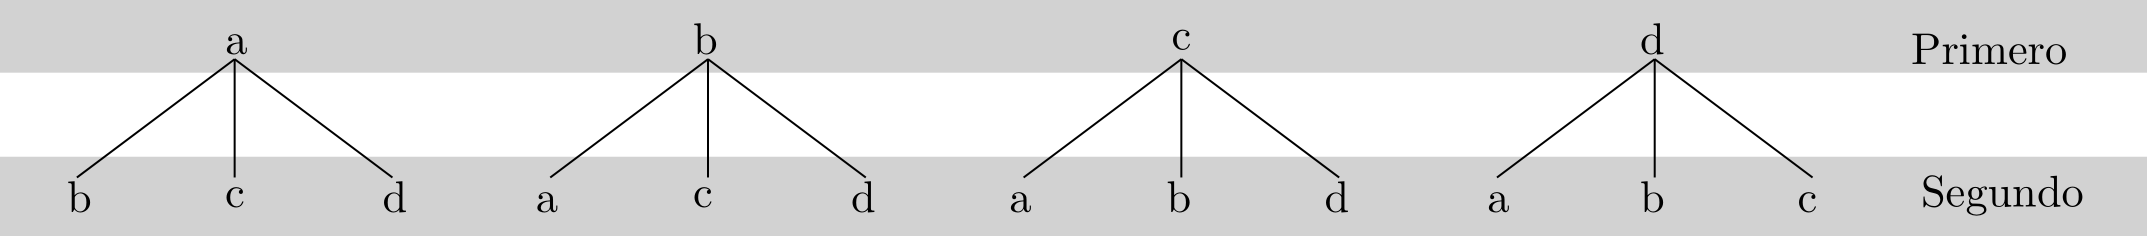
\includegraphics[width=13cm]{../fig/Cap03-Permutaciones42.pdf}
            \caption{Posibles primer y segundo puestos.}\label{cap03:fig:arbol2}
            \end{figure}
            \end{center}
        \item Es decir, de momento hemos contado $3+3+3+3=4\cdot 3$ casos diferentes.
            \begin{center}
            \begin{figure}[h!]	
            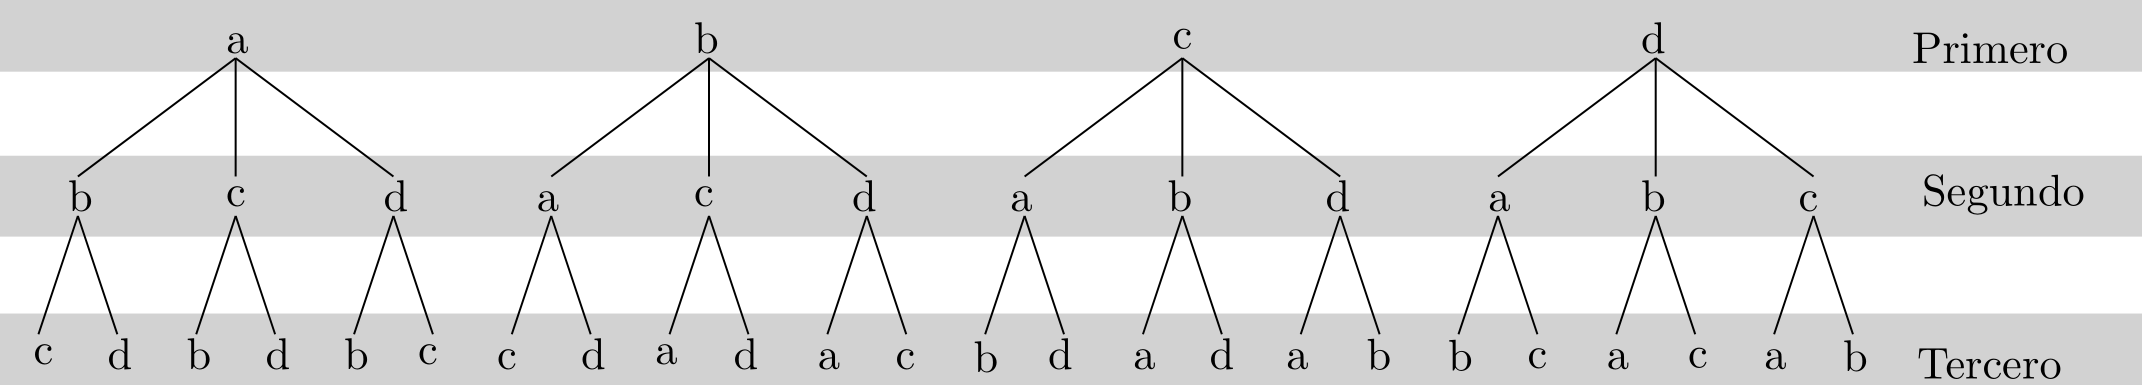
\includegraphics[width=13cm]{../fig/Cap03-Permutaciones43.pdf}
            \caption{Posibles tres primeros puestos.}\label{cap03:fig:arbol3}
            \end{figure}
            \end{center}
        \item Para la tercera posici\'on, y para cada uno de los casos del paso anterior, s\'olo podemos elegir a una de las dos personas que quedan. Por tanto, tenemos $4\cdot 3\cdot 2$ posibles colas diferentes, las que se muestran en la Figura \ref{cap03:fig:arbol3}. ¿Ves la forma del \'arbol (en las Figuras \ref{cap03:fig:arbol2} y \ref{cap03:fig:arbol3}?
        \item Para la \'ultima posici\'on s\'olo queda una persona: de hecho, no tenemos elección y obtenemos, en total, $4\cdot 3\cdot 2\cdot 1$ posibles colas distintas (Figura \ref{cap03:fig:arbol4}).
    		\begin{center}
            \begin{figure}[h!]	
            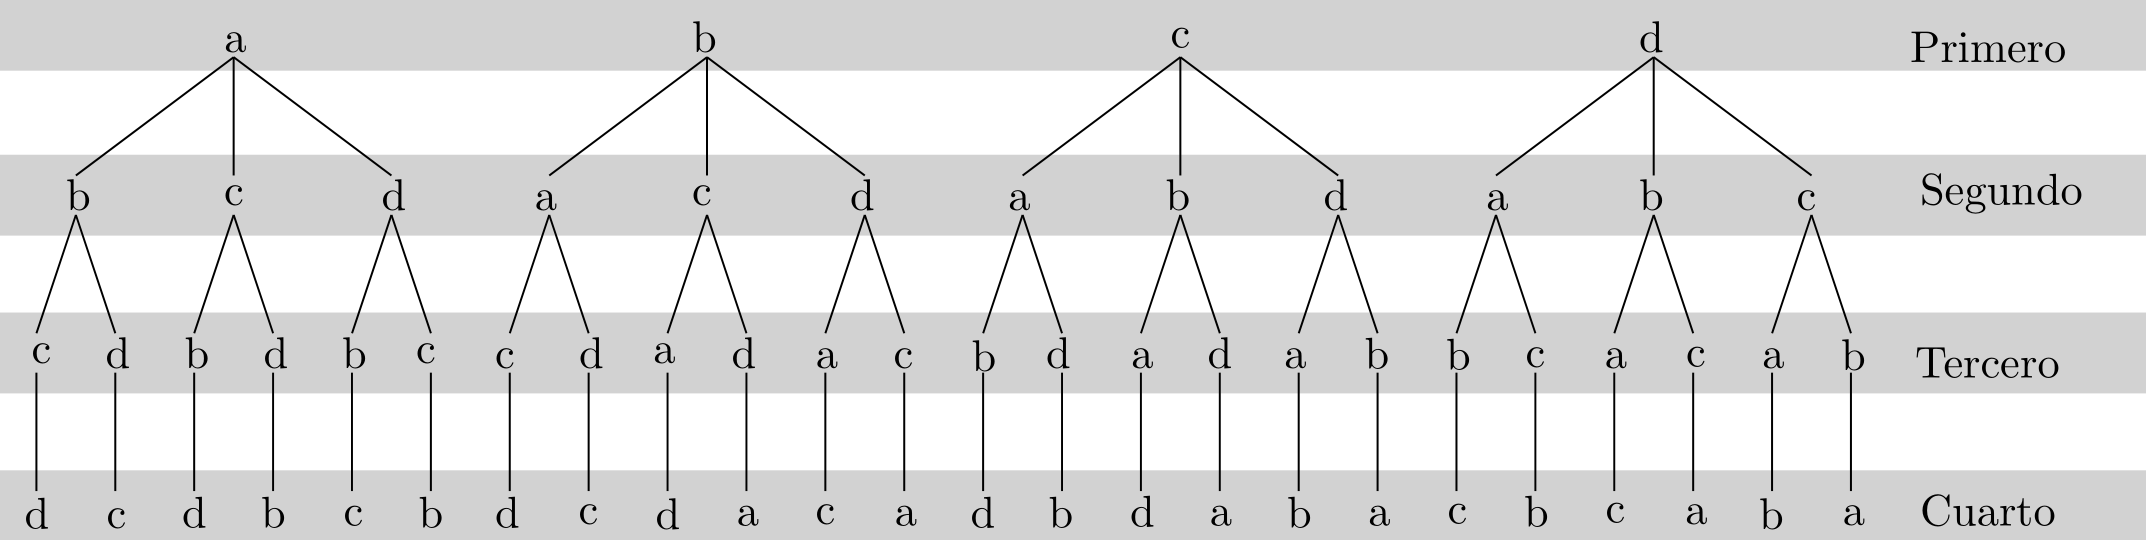
\includegraphics[width=13cm]{../fig/Cap03-Permutaciones44.pdf}
            \caption{Posibles colas}\label{cap03:fig:arbol4}
            \end{figure}
            \end{center}
    \end{itemize}
    En resumen, hay\, $24=4\cdot 3\cdot 2\cdot 1$ colas distintas posibles con cuatro personas.\qed
    \end{Ejemplo}
Si has entendido lo anterior, verás que no es dif\'icil extender el razonamiento a una cola con un n\'umero {\em arbitrario} de individuos. Para expresar el número de permutaciones de $n$ elementos es muy \'util el concepto de {\sf factorial}\index{factorial}.
    \begin{center}
    \fcolorbox{black}{Gris025}{
    \begin{minipage}{8cm}
        {\centering \bf El factorial de $n=1,2,3,\ldots$ es:}
            \[n!=n\cdot(n-1)\cdot(n-2)\cdot\,\ldots\,\cdot3\cdot 2\cdot 1.\]
    \end{minipage}}
    \end{center}
Es decir, el producto de todos los números entre $1$ y $n$. Por ejemplo,
\[10!=10\cdot 9\cdot 8\cdot 7\cdot 6\cdot 5\cdot 4\cdot 3\cdot 2\cdot 1=3628800.\]
(Con diez personas, hay más de tres millones de colas distintas posibles). Además definimos el factorial de $0$ como un caso especial:
    \begin{center}
    \fcolorbox{black}{Gris025}{
    \begin{minipage}{2cm}
        {\centering $0!=1.$}
    \end{minipage}}
    \end{center}
La propiedad más llamativa del factorial es su crecimiento extremadamente rápido. Por ejemplo, $100!$ es del orden de $10^{57}$. Este comportamiento
está detrás del fenómeno que se conoce habitualmente como {\sf explosión combinatoria}\index{explosión combinatoria}, en el que empezamos con pocos
elementos, pero al estudiar las listas o subconjuntos formados a partir de esos elementos, los problemas se vuelven rápidamente intratables por su tamaño.

En resumen, el número de permutaciones de $n$ elementos, esto es, el n\'umero de {\sf distintas formas de ordenar} los elementos de un conjunto de $n$ elementos viene dado por
    \begin{center}
    \fcolorbox{black}{Gris025}{
    \begin{minipage}{8cm}
        {\centering \bf Permutaciones de $n$ elementos}
            \[\operatorname{Per}(n)=n!=n\cdot(n-1)\cdot(n-2)\cdot\,\ldots\,\cdot3\cdot 2\cdot 1.\]
    \end{minipage}}
    \end{center}


\subsection{Variaciones.}
\label{cap03:subsec:variaciones}

El problema que abordaremos a continuación est\'a muy relacionado con las permutaciones.
Dado un conjunto de $n$ elementos distintos, queremos saber el número de subconjuntos ordenados que podemos hacer con $k$ de sus elementos, donde $0<k<n$. Empezamos con un ejemplo:

\begin{Ejemplo} En una carrera en la que participan $7$ corredores,
de cu\'antas formas posibles pueden repartirse los $3$ primeros puestos?
Recapitulemos:
\begin{itemize}
	\item De nuevo el orden es importante (no es lo mismo ser el primero
		que el tercero).
	\item Ahora NO usaremos todos los elementos (participantes).
	\item Cada corredor, l\'ogicamente, puede aparecer como mucho una vez entre los tres mejores.
\end{itemize}
El razonamiento es esencialmente an\'alogo al que nos llev\'o a deducir la
f\'ormula para las permutaciones. La diferencia es que ahora nos detendremos
en el tercer ``nivel'', puesto que s\'olo nos interesan los tres primeros puestos.
En total hay $7\cdot 6 \cdot 5 =210$ posibles podios.\qed
\end{Ejemplo}
Vamos a poner nombre a estas listas ordenadas: diremos que cada una de ellas es una
{ \sf variaci\'on de $7$ elementos tomados de $3$ en $3$}.

En el lenguaje de los n\'umeros factoriales, podemos expresar esto así. El número de variaciones de $7$ elementos, tomados de $3$ en $3$ es
    	\[\operatorname{V}(7,3)=7\cdot\cdot 6 \cdot 5=\dfrac{7!}{(7-3)!}.\]
Merece la pena detenerse unas lineas en la \'ultima igualdad,
que analizaremos a través de un ejemplo:
\[\begin{array}{rl}
\operatorname{V}(7,4)=7\cdot 6\cdot 5 & =
\dfrac{7 \cdot 6 \cdot 5 \cdot 4 \cdot \cdots \cdot 2 \cdot 1}{4 \cdot \cdots \cdot 2 \cdot 1}\\
	& \\
	& =\dfrac{7!}{(7-3)!}\\
\end{array}
\]
Si leemos esta ecuación de izquierda a derecha, lo que hemos hecho ha sido multiplicar y dividir por la misma cantidad, hasta completar el factorial de $7$ en el numerador. %Si vamos de derecha a izquierda, el mecanismo ha sido el de simplificar algunos factores del numerador con (todos) los del denominador.
%
%{\bf Sin repetici\'on} Listas de $k$ elementos entre $n$ posibles, sin repetir
%elementos y considerando distintas dos listas si el orden de los elementos es distinto.
%\fobox{\operatorname{V}(n,k)=n\cdot(n-1)\cdot\dots\cdot(n-k+1)=\dfrac{n!}{(n-k)!}}
Lo interesante de este truco es que nos permite escribir el caso general de una forma muy compacta:
    \begin{center}
    \fcolorbox{black}{Gris025}{
    \begin{minipage}{10cm}
        {\centering \bf Variaciones de $n$ elementos, tomados de $k$ en $k$}
            \[\operatorname{V}(n,k)=n\cdot(n-1)\cdot\dots\cdot(n-k+1)=\dfrac{n!}{(n-k)!}.\]
    \end{minipage}}
    \end{center}
%
%	 \begin{center}
%        \fbox{\colorbox{Gris025}{
%        \begin{minipage}{9cm}
%        		 \begin{center}
%        {\bf Variaciones de $n$ elementos, tomados de $k$ en $k$
%        \index{Variaciones de $n$ elementos, tomados de $k$ en $k$}}%\\[3mm]
%        		 \end{center}
%		\[\operatorname{V}(n,k)=n\cdot(n-1)\cdot\dots\cdot(n-k+1)=\dfrac{n!}{(n-k)!}.\]
%       \end{minipage}}
%        }
%    \end{center}
Para intentar aclarar la relación entre ambos conceptos, podemos ver las permutaciones de $n$ elementos como un caso particular de las variaciones, en el que tomamos $k=n$ elementos.

\subsection{Combinaciones.}
\label{cap03:subsec:Combinaciones}

Tanto en las permutaciones como en las variaciones, el orden en que aparecen los elementos es
importante. Ahora nos vamos a olvidarnos de \'el. Esto recuerda a juegos de apuestas como las de la
{\em Loter\'ia Primitiva} en España (descrita en detalle en el enlace [\,\ref{enlace0008}\,]\label{enlace0008a}). En este tipo de juegos da igual el orden en el que salgan los n\'umeros, lo importante es que coincidan con nuestra apuesta.
	
Estamos interesados en este problema. Dado un conjunto de $n$ elementos
    \[A=\{x_1,x_2,\ldots,x_n\}\]
y un número $k$ con $0\leq k\leq n$, ¿cuántos {\sf subconjuntos distintos} de $k$ elementos podemos formar con los elementos de $A$? Es muy importante entender que, como ya hemos anunciado, al usar la palabra \index{subconjunto}{\sf subconjunto}, estamos diciendo que:
    \begin{enumerate}
        \item el {\sf orden de los elementos es irrelevante}. El subconjunto $\{x_1,x_2,x_3\}$ es el mismo que el subconjunto $\{x_3,x_1,x_2\}$.
        \item los elementos del subconjunto {\sf no se repiten}. El subconjunto $\{x_1,x_2,x_2\}$ es, de hecho, igual al subconjunto $\{x_1,x_2\}$ (y nunca lo escribiríamos de la primera manera, si estamos hablando de subconjuntos).
    \end{enumerate}
Vamos a ponerle un nombre a lo queremos calcular: el número de subconjuntos posibles es el número de   \index{combinaciones de $n$ elementos, tomados de $k$ en $k$}{\sf combinaciones de $n$ elementos, tomados de $k$ en $k$} (cada uno de los subconjuntos es una combinación). Para hacer este c\'alculo, volvamos un momento sobre las variaciones de $n$ elementos, tomados de $k$ en $k$.
Esto no deber\'ia sorprendernos (y no digo que lo haga) porque en ambos casos tenemos un total de $n$ elementos y hacemos subgrupos con $k$ de ellos. Sin embargo
    \begin{itemize}
    \item En el caso de las combinaciones el orden no es importante.
    \item Por el contrario, en cuanto a variaciones se refiere,
    contabilizamos como variaciones diferentes (porque lo son) aquellas que
    tienen los mismos $k$ elementos ordenados de distinta forma.
    \end{itemize}
Con la experiencia adquirida con permutaciones y variaciones, no necesitamos
pasar por un ejemplo previo.

Si nos fijamos en que en un caso el orden es importante y en el otro no, resulta que por cada combinaci\'on (subconjunto de $k$ elementos) tenemos $k!$ variaciones (el n\'umero de formas distintas de ordenar esos $k$ elementos). Dicho de otro modo, fijados $n$ y $k$, hay $k!$ más variaciones que combinaciones. De ahí deducimos que
\[C(n,k)\cdot k! = V(n,k)\]
Si recordamos la fórmula que nos permitía calcular $V(n,k)$, podemos despejar
de la igualdad anterior $C(n,k)$ y obtener una fórmula para el número de combinaciones.
    \begin{center}
    \fcolorbox{black}{Gris025}{
    \begin{minipage}{10cm}
        {\centering \bf Combinaciones de $n$ elementos, tomados de $k$ en $k$}
        \[C(n,k)=\dfrac{n!}{k!(n-k)!},\]
        para $0\leq k\leq n$, y $n=0,1,2\ldots$ cualquier número natural.
    \end{minipage}}
    \end{center}

\subsection{Números combinatorios.}
\label{cap03:subsec:NumerosCombinatorios}

Los números combinatorios\index{números combinatorios}\index{combinatorios, números} son una expresión alternativa, y muy útil, de las combinaciones:
    \begin{center}
    \fcolorbox{black}{Gris025}{
    \begin{minipage}{10cm}
        {\centering \bf Números combinatorios}\\
        El número combinatorio $n$ sobre $k$ es
        \[\binom{n}{k}=\dfrac{n!}{k!(n-k)!},\]
        para $0\leq k\leq n$, y $n=0,1,2\ldots$ cualquier número natural.
    \end{minipage}}
    \end{center}
%
%     \begin{center}%\\[3mm]
%        \fbox{\colorbox{Gris025}{\begin{minipage}{14cm}
%       \begin{center}
%        %\vspace{2mm}
%         {\bf Números combinatorios:} en número combinatorio $n$ sobre $k$ es
%       \end{center}
%        \[\binom{n}{k}=\dfrac{n!}{k!(n-k)!}\mbox{, \quad para $0\leq k\leq n$, y $n=0,1,2\ldots$ cualquier número natural}\]
%        %\quad
%        \end{minipage}}}
%        \end{center}%\\[3mm]




%    \item Para calcular probabilidades de forma eficaz muchas veces necesitamos una manera de calcular el número de combinaciones posibles. El \index{Número combinatorio}{\sf número combinatorio} $\binom{n}{k}$ es el número de combinaciones de $n$ elementos tomados de $k$ en $k$.
%
%    \item Para calcular ese número necesitamos el concepto de {\sf factorial}. El factorial del número $n$ es el producto
%        \[\fbox{\colorbox{Gris025}{$n!=n\cdot(n-1)\cdot(n-2)\cdot\,\ldots\,\cdot3\cdot 2\cdot 1.$}}\]
%        Es decir, el producto de todos los números entre $1$ y $n$. Además definimos \fbox{$0!=1$}. Por ejemplo, se tiene:
%        \[6!=6\cdot 5\cdot 4\cdot 3\cdot 2\cdot 1=720.\]
%        La propiedad más llamativa del factorial es su crecimiento extremadamente rápido. Por ejemplo, $100!$ es del orden de $10^{57}$.
%
%    \item La fórmula de los números combinatorios es esta:
%     \begin{center}%\\[3mm]
%        \fbox{\colorbox{Gris025}{\begin{minipage}{14cm}
%        %\begin{center}
%        %\vspace{2mm}
%        {\bf Números combinatorios:}
%        %\end{center}
%        \[\binom{n}{k}=\dfrac{n!}{k!(n-k)!}\mbox{, \quad para $0\leq k\leq n$, y $n=0,1,2\ldots$ cualquier número natural}\]
%        %\quad
%        \end{minipage}}}
%        \end{center}%\\[3mm]
%        Por ejemplo, el número de combinaciones del Ejemplo \ref{ejem:combinacionesCuatroDosEnDos} es
%        \[\binom{4}{2}=\dfrac{4!}{2!(4-2)!}=\dfrac{24}{2\cdot 2}=6,\]
%        como era de esperar.

Hay dos observaciones que facilitan bastante el trabajo con estos números combinatorios.
    \begin{itemize}
        \item Los números combinatorios se pueden representar en esta tabla de forma triangular, llamada el {\sf Triángulo de Pascal}:
        \begin{equation}\label{cap03:ecu:TrianguloPascal}
        \begin{array}{l|llcccccccccccccc}
        n=0&&&&&&&&&1\\
        n=1&&&&&&&&1&&1\\
        n=2&&&&&&&1&&2&&1\\
        n=3&&&&&&1&&3&&3&&1\\
        n=4&&&&&1&&4&&6&&4&&1\\
        n=5&&&&1&&5&&10&&10&&5&&1\\
        n=6&&&1&&6&&15&&20&&15&&6&&1\\
        \vdots&&& &&\vdots&& &&\vdots&& &&\vdots&&
        \end{array}
        \end{equation}
        El número $\binom{n}{k}$ ocupa la fila $n$ posición $k$ (se cuenta desde $0$). Por ejemplo en la $4$ fila, posición $2$ está nuestro viejo conocido $\binom{4}{2}=6$. ¿Cuánto vale $\binom{5}{3}$?

        Los puntos suspensivos de la parte inferior están ahí para indicarnos qué podríamos seguir, y a la vez para servir de desafío. ¿Qué viene a continuación? ¿Qué hay en la línea $n=15$? Pues parece claro que empezará y acabará con un $1$. También parece claro que el segundo y el penúltimo  número valen $7$. ¿Pero y el resto? Lo que hace especial a esta tabla es que {\sf cada número que aparece en el interior de la tabla es la suma de los dos situados a su izquierda y derecha en la fila inmediatamente superior.} Por ejemplo, el $10$ que aparece en tercer lugar en la fila de $n=5$  es la suma del $4$ y el $6$ situados sobre él en la  segunda y tercera posiciones de la fila para $n=4$. Con esta información, podemos obtener la séptima fila de la tabla, a partir de la sexta, sumando según indican las flechas en este esquema:
        {\small
        \[
        \begin{array}{lcccccccccccccccc}
        &&1&&6&&15&&20&&15&&6&&1\\
           &&\swarrow\searrow&&\swarrow\searrow&&\swarrow\searrow&&\swarrow\searrow&&\swarrow\searrow&&
           \swarrow\searrow&&\swarrow\searrow\\
        &1&&7&&21&&35&&35&&21&&7&&1
        \end{array}
        \]
        }
        \item La segunda observación importante sobre los números combinatorios quedará más clara con un ejemplo:
        \[
        \binom{12}{7}=\dfrac{12!}{7!(12-7)!}=\dfrac{12!}{7!5!}.
        \]
        Ahora observamos que $12!=(12\cdot 11\cdot\cdots\cdot 6)\cdot(5\cdot\cdots\cdot 2\cdot 1)$, y los paréntesis muestran que esto
        es igual a $(12\cdot 11\cdot\cdots\cdot 6)\cdot 5!$. Este factorial de $5$ se cancela con el del denominador y tenemos
        \[
        \binom{12}{7}=\dfrac{\overbrace{12\cdot 11\cdot 10\cdot 9\cdot 8\cdot 7\cdot 6}^{6\mbox{ factores}}}{7!}=792.
        \]
        Generalizando esta observación sobre la cancelación de factoriales, la forma en la que vamos a expresar los coeficientes binomiales será finalmente esta:
        \begin{equation}\label{cap03:ecu:expresionPseudoFactorialCoeficientesBinomiales}
        \dbinom{n}{k}=\frac{\overbrace{n\left( n-1\right) \left( n-2\right) \cdots \left( n-k+1\right) }^{k\mbox{ factores}}}{k!}
        \end{equation}
        Y, como hemos indicado, lo que caracteriza este esta expresión es que tanto el numerador como el denominador tienen $k$ factores.
    \end{itemize}
Los números combinatorios son importantes en muchos problemas de probabilidad. Veamos un par de ejemplos:
    \begin{Ejemplo}
    \label{cap03:ejem:BombillasDefectuosas}
    Tenemos una caja de 10 bombillas y sabemos que tres están fundidas. Si sacamos al azar tres bombillas de la caja\footnote{``al azar'' aquí significa que todos los subconjuntos de tres bombillas son equiprobables.}, ¿Cuál es la probabilidad de que hayamos sacado las tres que están fundidas?\\[2mm]
    En este caso, al tratar de aplicar la Regla de Laplace, usamos los números combinatorios para establecer el número de casos posibles. ¿Cuántas formas distintas hay de seleccionar tres bombillas de un conjunto de 10? Evidentemente hay $\binom{10}{3}$ formas posibles. Este número es:
    \[\binom{10}{3}=\dfrac{10\cdot 9\cdot 8}{3\cdot 2\cdot 1}=120.\]
    Estos son los casos posibles. Está claro además que sólo hay un caso favorable, cuando elegimos las tres bombillas defectuosas. Así pues, la probabilidad pedida es:
    \[\dfrac{1}{120}.\]
    \qed
    \end{Ejemplo}
El siguiente ejemplo es {\sf\em extremadamente importante} para el resto del curso, porque nos abre la puerta que nos conducirá a la Distribución Binomial (que veremos en el Capítulo \ref{cap:TeoremaCentralLimite}) y a algunos de los resultados más profundos de la Estadística.
    \begin{Ejemplo}
    \label{cap03:ejem:probabilidadLanzamientoMonedas}
    Lanzamos una moneda al aire cuatro veces, y contamos el número de caras obtenidas en esos lanzamientos. ¿Cuál es la probabilidad de obtener exactamente dos caras en total?\\
    Vamos a pensar en cuál es el espacio muestral. Se trata de listas de cuatro símbolos: cara o cruz. Por ejemplo,
    \[\smiley\smiley\dagger\smiley\]
    es un resultado posible, con tres caras y una cruz. ¿Cuántas de estas listas de cara y cruz con cuatro símbolos hay? Enseguida se ve que hay $2^4$, así que ese es el número de casos posibles. ¿Y cuál es el número de casos favorables? Aquí es donde los números combinatorios acuden en nuestra ayuda. Podemos pensar así en los sucesos favorables: tenemos cuatro fichas, dos caras y dos cruces $\smiley,\smiley,\dagger,\dagger,$ y un casillero con cuatro casillas
    \begin{center}
    \begin{tabular}{|c|c|c|c|}
    \hline
     \rule{0cm}{0.5cm}\rule{1cm}{0cm}&\rule{1cm}{0cm}&\rule{1cm}{0cm} &\rule{1cm}{0cm}\\
     \hline
     \end{tabular}
     \end{center}
     en las que tenemos que colocar esas cuatro fichas. Cada manera de colocarlas corresponde a un suceso favorable. Y entonces está claro que lo que tenemos que hacer es elegir, de entre esas cuatro casillas, cuáles dos llevarán una cara (las restantes dos llevarán una cruz). Es decir, hay que elegir dos de entre cuatro. Y ya sabemos que la respuesta es $\binom{4}{2}=6$. Por lo tanto la probabilidad pedida es:
     \[P(2 \mbox{ caras} )=\dfrac{\binom{4}{2}}{2^4}=\binom{4}{2}\left(\dfrac{1}{2}\right)^4=\dfrac{6}{16}.\]
     Supongamos ahora que lanzamos la moneda $n$ veces y queremos saber cuál es la probabilidad de obtener $k$ veces cara. Un razonamiento similar produce la fórmula:
    \[P(k \mbox{ caras})=\binom{n}{k}\left(\dfrac{1}{2}\right)^n.\]
    \qed
    \end{Ejemplo}

En relación con este ejemplo, y con la vista puesta en el trabajo que haremos con la Distribución Binomial, no queremos dejar de mencionar que los números combinatorios son también importantes en relación con el Teorema del Binomio, y que por eso se los conoce también como {\sf coeficientes binomiales}\index{coeficientes binomiales}\index{binomiales, coeficientes}. En concreto, se tiene, para $a,b\in\R$, y $n\in\N$ esta {\sf Fórmula del Binomio}\index{binomio, fórmula del}\index{fórmula del binomio}:
 \begin{equation}\label{cap03:ecu:FormulaBinomio}
 (a+b)^n=\binom{n}{0}a^n+\binom{n}{1}a^{n-1}b+\binom{n}{2}a^{n-2}b^2+\cdots+\binom{n}{n-1}ab^{n-1}+\binom{n}{n}b^n
  \end{equation}
El lector conocerá, sin duda, el caso $n=2$, que es la fórmula para el cuadrado de una suma:
\[(a+b)^2=a^2+2ab+b^2.\]
Dejamos como ejercicio comprobar que esto es exactamente lo que dice la Fórmula del Binomio para $n=2$. Asimismo, le pedimos al lector que compruebe que:
\[(a+b)^3=a^3+3a^2b+3ab^2+b^3.\]
Y que haga el mismo ejercicio para $n=4$ y $n=5$ (es de mucha ayuda mirar las filas dle triángulo de Pascal, pág. \pageref{cap03:ecu:TrianguloPascal}).

\subsection{Otras fórmulas combinatorias.}
\label{cap03:subsec:OtrasFormulasCombinatorias}
{\bf Atención:}
Aunque las incluimos aquí para complementar la información de este capítulo, {\bf excepto} la de las variaciones con repetición (que por otra parte es la más sencilla), las fórmulas de este apartado son mucho menos importantes para nosotros que las precedentes.
%De hecho, deberías poder deducir esta fórmula a partir del razonamiento que nos llevó a la expresión que permite calcularlas variaciones de $n$ elementos, tomados de $k$ en $k$.

Vamos a ver los análogos de los objetos que hemos estudiado (permutaciones, variaciones, combinaciones), cuando se permite los elementos pueden aparecer repetidos.
    \begin{center}
    \fcolorbox{black}{Gris025}{
    \begin{minipage}{10cm}
        {\centering \bf Permutaciones con repetición de $n$ elementos\index{permutaciones con repetici\'on}}\\
        El n\'umero de permutaciones que se pueden formar con $m$ objetos
        entre los cuales hay $n_1$ iguales entre s\'{\i}, otros $n_2$ iguales
        entre s\'{\i},\dots, y finalmente $n_k$ iguales entre s\'{\i}, es:
        %\end{center}
        \begin{equation}\label{cap03:ecu:PermutacionesConRepeticion}
        \operatorname{PerRep}(n_1,n_2,\cdots,n_k)=\dfrac{m!}{n_1!n_2!\cdots n_k!}
        \end{equation}
        Obsérvese que ha de ser, necesariamente:
        \[m=n_1+n_2+\cdots+n_k.\]
    \end{minipage}}
    \end{center}
    Por ejemplo, si tenemos la lista $[a,a,b,b,c]$, es decir $m=5$, $n_1=2$ (hay dos repeticiones de $a$), $n_2=2$ y $n_3=1$, entonces hay:
    \[\operatorname{PerRep}(2,2,1)=\dfrac{5!}{2!\cdot 2!\cdot 1!}=30.\]
    En la Tabla \ref{cap03:tabla:permutacionesRepeticion} (pág. \pageref{cap03:tabla:permutacionesRepeticion}) pueden verse esas 30 permutaciones.

    \begin{center}
    \fcolorbox{black}{Gris025}{
    \begin{minipage}{10cm}
        {\centering \bf Variaciones con repetición de $n$ elementos, tomados de $k$ en $k$\index{variaciones con repetici\'on}}\\
        Si se permite que cada elemento aparezca tantas veces como se quiera, entonces:
        \begin{equation}\label{cap03:ecu:VariacionesConRepeticion}
        \operatorname{VRep}(n,k)=n^k
        \end{equation}
    \end{minipage}}
    \end{center}
    Por ejemplo, con los 3 elementos $[a,b,c]$, tomados de dos en dos, y permitiendo repeticiones obtenemos las
    \[\operatorname{VRep}(3,2)=3^2=9\]
    permutaciones con repetición que pueden verse en la Tabla \ref{cap03:tabla:variacionesRepeticion}.
        \begin{table}[ht]
        \centering
        \begin{tabular}{lllllllll}
          \hline
          1 & 2 & 3 & 4 & 5 & 6 & 7 & 8 & 9 \\
          \hline
            a & a & a & b & b & b & c & c & c \\
            a & b & c & a & b & c & a & b & c \\
           \hline
        \end{tabular}
        \caption{Las 9 variaciones con repetición de los elementos $[a,b,c]$, tomados de 2 en 2}.\label{cap03:tabla:variacionesRepeticion}
        \end{table}
    De hecho, ya hemos visto otro caso similar en el Ejemplo \ref{cap03:ejem:probabilidadLanzamientoMonedas}. Con los dos símbolos $\smiley$ y $\dagger$, para rellenar cuatro casillas (con repeticiones) se pueden formar
    \[\operatorname{VRep}(3,2)=2^4=16\]
    variaciones con repetición.

    \begin{center}
    \fcolorbox{black}{Gris025}{
    \begin{minipage}{10cm}
        {\centering \bf Combinaciones con repetición  de $n$ elementos, tomados de $k$ en $k$\index{combinaciones con repetici\'on}}\\
         Selecciones de $k$ elementos entre $n$ posibles,
         admitiendo la repetici\'on de elementos, pero sin tener en cuenta el orden de la selecci\'on.
        \begin{equation}\label{cap03:ecu:CombinacionesConRepeticion}
        \operatorname{CRep}(n,k)=\binom{n+k-1}{k}
        \end{equation}
    \end{minipage}}
    \end{center}
    Si tomamos los elementos $[a,b,c,d]$ y formamos las combinaciones con repetición de estos elementos, tomados de tres en tres, obtendremos las:
    \[\operatorname{CRep}(4,3)=\binom{4+3-1}{3}=20\]
    combinaciones, que pueden verse en la Tabla \ref{cap03:tabla:CombinacionesRepeticion}.


\begin{table}[ht]
\centering
\begin{tabular}{rrrrrr}
  \hline
1 & a & a & b & b & c \\
  2 & a & a & b & c & b \\
  3 & a & a & c & b & b \\
  4 & a & b & a & b & c \\
  5 & a & b & a & c & b \\
  6 & a & b & b & a & c \\
  7 & a & b & b & c & a \\
  8 & a & b & c & a & b \\
  9 & a & b & c & b & a \\
  10 & a & c & a & b & b \\
  11 & a & c & b & a & b \\
  12 & a & c & b & b & a \\
  13 & b & a & a & b & c \\
  14 & b & a & a & c & b \\
  15 & b & a & b & a & c \\
  16 & b & a & b & c & a \\
  17 & b & a & c & a & b \\
  18 & b & a & c & b & a \\
  19 & b & b & a & a & c \\
  20 & b & b & a & c & a \\
  21 & b & b & c & a & a \\
  22 & b & c & a & a & b \\
  23 & b & c & a & b & a \\
  24 & b & c & b & a & a \\
  25 & c & a & a & b & b \\
  26 & c & a & b & a & b \\
  27 & c & a & b & b & a \\
  28 & c & b & a & a & b \\
  29 & c & b & a & b & a \\
  30 & c & b & b & a & a \\
   \hline
\end{tabular}
\caption{Las 30 permutaciones con repetición de $[a,a,b,b,c]$}\label{cap03:tabla:permutacionesRepeticion}
\end{table}

\begin{table}[ht]
\centering
\begin{tabular}{rlll}
  \hline
 & 1 & 2 & 3 \\
  \hline
1 & a & a & a \\
  2 & a & a & b \\
  3 & a & a & c \\
  4 & a & a & d \\
  5 & a & b & b \\
  6 & a & b & c \\
  7 & a & b & d \\
  8 & a & c & c \\
  9 & a & c & d \\
  10 & a & d & d \\
  11 & b & b & b \\
  12 & b & b & c \\
  13 & b & b & d \\
  14 & b & c & c \\
  15 & b & c & d \\
  16 & b & d & d \\
  17 & c & c & c \\
  18 & c & c & d \\
  19 & c & d & d \\
  20 & d & d & d \\
   \hline
\end{tabular}
\caption{Combinaciones con repetición de $[a,b,c,d]$, tomados de tres en tres.}\label{cap03:tabla:CombinacionesRepeticion}.
\end{table}





\subsubsection{Los juegos del caballero De Méré, solución combinatoria}
\label{cap03:subsubsec:JuegosDeMereCombinatoria}

Vamos a utilizar estas fórmulas para responder, de una manera fácil, a los dos experimentos (a) y (b) del Caballero De Méré (ver apartado \ref{PrimerasNocionesProbabilidad}, pág. \pageref{PrimerasNocionesProbabilidad}).

\begin{Ejemplo}{El primer juego de De Méré}\label{cap03:ejem:DeMere01}
    Recordemos que, en este juego, se trata de calcular la probabilidad de obtener al menos un seis en cuatro lanzamientos de un dado. Para usar la Regla de Laplace debemos empezar por considerar todos los resultados elementales (y equiprobables) posibles. Es decir, todas las listas posibles (incluyendo repeticiones, y teniendo en cuenta el orden) de  cuatro números, formadas con los números del 1 al 6. La combinatoria que hemos aprendido en esta Sección dice que hay
    \[\operatorname{VRep}(6,4)=6^4=1296.\]
    de esas listas. De ellas, las que {\em no contienen} ningún 6 son todas las listas posibles (incluyendo repeticiones, y teniendo en cuenta el orden) de cuatro números,  formadas con los números del 1 al 5. De estas, hay:
    \[\operatorname{VRep}(5,4)=5^4=625.\]
    Y ahora la Regla de Laplace dice que la probabilidad que queremos calcular es:
    \[1-\dfrac{625}{1296}\approx 0.5178,\]
    con cuatro cifras significativas.
\end{Ejemplo}

\begin{Ejemplo}{El segundo juego de De Méré}\label{cap03:ejem:DeMere02}
    En este segundo juego, se trata de calcular la probabilidad de obtener al menos un seis doble en veinticuatro lanzamientos de un par de dados. Para usar la Regla de Laplace, empezamos considerando todas las listas posibles (incluyendo repeticiones, y teniendo en cuenta el orden) de  24 números, formadas con los números del 1 al 36 (los 36 resultados equiprobables posibles al lanzar dos dados). La combinatoria que hemos aprendido en esta Sección dice que hay
    \[\operatorname{VRep}(36,24)=36^{24}=22452257707354557240087211123792674816\]
    de esas listas. Por cierto, ¿podrías calcular esto usando una calculadora? De ellas, las que {\em no contienen} ningún 6 doble son todas las listas posibles (incluyendo repeticiones, y teniendo en cuenta el orden) de 24 números,  formadas con los números del 1 al 35. De estas, hay:
    \[\operatorname{VRep}(35,24)=35^{24}=11419131242070580387175083160400390625.\]
    Y ahora la Regla de Laplace dice que la probabilidad que queremos calcular es:
    \[1-\dfrac{\operatorname{VRep}(35,24)}{\operatorname{VRep}(36,24)}\approx 0.4914,\]
    con cuatro cifras significativas. Este es un buen momento para volver a ver los resultados de las simulaciones que se incluyen el Tutorial03, y ver si se corresponden con lo que predice la teoría.\qed
\end{Ejemplo}

\newpage
\section{Posibilidades (odds) y el lenguaje de las pruebas diagnósticas.}
\label{cap03:sec:OddsPruebasDiagnosticas}
\noindent{\bf Opcional: esta sección puede omitirse en una primera lectura.}\\

En esta sección vamos a introducir el concepto de {\sf posibilidades}\index{posibilidades (odds)} (en inglés, {\em odds}\index{odds}). Lo haremos dentro del contexto de las pruebas diagnósticas que hemos esbozado en los Ejemplos \ref{cap03:ejem:PruebasDiagnosticas01} (pág. \pageref{cap03:ejem:PruebasDiagnosticas01})y \ref{cap03:ejem:PruebasDiagnosticasBayes} (pág. \pageref{cap03:ejem:PruebasDiagnosticasBayes}), en el que ese concepto se utiliza a menudo. Y vamos a aprovechar para introducir parte de la terminología estadística más básica que se usa en esas pruebas. No obstante, aunque presentamos el concepto de posibilidades (odds) en este contexto, queremos subrayar que sus aplicaciones son mucho más amplias, como veremos más adelante en el curso.

\subsection{Prevalencia, sensibilidad y especificidad.}
\label{cap03:subsec:PrevalenciaSensibilidad}

El modelo clásico de prueba diagnóstica consiste  en algún tipo de procedimiento que permite detectar la presencia o ausencia de una cierta enfermedad. O, más en general, de cualquier otra circunstancia; una prueba de embarazo es una prueba diagnóstica, en este sentido. Simplificando, en esta sección vamos a hablar de {\em enfermedad} en cualquier caso. Para aplicar el lenguaje de la Probabilidad en este contexto, empezamos por llamar {\sf prevalencia}\index{prevalencia} de la enfermedad a la probabilidad de que un individuo, tomado al azar de la población que nos interesa, esté enfermo. En inglés {\em disease} significa {\em enfermedad}, y por eso vamos a utilizar el símbolo $P(D)$ para referirnos a la prevalencia.

Cuando se utiliza una prueba diagnóstica en una población, en la cual hay una parte de los individuos afectados por una enfermedad,  hay dos sucesos básicos que nos interesan: por un lado, el suceso $D$ que ya hemos presentado, y que indica la presencia o ausencia de la enfermedad. Y, por otro lado, el suceso que indica el resultado positivo o negativo de la prueba, y que indicaremos con los símbolos $+$ y $-$, respectivamente.

Vamos a utilizar de nuevo el lenguaje de las {\em tablas de contingencia}, que ya vimos en esos ejemplos, para describir el resultado de las pruebas diagnósticas. La tabla de contingencia adecuada es una tabla de doble entrada, como la Tabla \ref{cap03:tabla:notacionTablaContingencia}

\begin{table}[ht]
        \begin{center}
        \begin{tabular}{cc|c|c|c|}
              &\multicolumn{1}{c}{}&\multicolumn{3}{c}{\bf Enfermedad:}\\
              \cline{3-5}
              % after \\: \hline or \cline{col1-col2} \cline{col3-col4} ...
               &\multicolumn{1}{c|}{}& Enfermos $D$&  Sanos $D^c$& Total \\
               \cline{2-5}
        {\bf Resultado de la prueba:}&\multicolumn{1}{|c|}{Positivo $+$}& $n_{11}$ & $n_{12}$ & $n_{1+}$ \\ % 11 8 19
              \cline{2-5}
             & \multicolumn{1}{|c|}{Negativo $-$}& $n_{21}$ & $n_{22}$ &  $n_{2+}$\\ % 4  7 11
              \cline{2-5}
             & \multicolumn{1}{|c|}{Total} & $n_{+1}$ & $n_{+2}$ & $n$ \\
              \cline{2-5}
        \end{tabular}
        \end{center}
\caption{Notación para las tablas de contingencia de una prueba diagnóstica}
\label{cap03:tabla:notacionTablaContingencia}
\end{table}
La notación que usamos para los totales que aparecen en los márgenes de la tabla, y a los que nos referiremos como {\sf valores marginales}\index{marginales, valores}\index{valores, marginales} es esta:
\[
\begin{cases}
n_{1+}=n_{11}+n_{12},&\mbox{ suma de la primera fila, total de positivos}.\\[2mm]
n_{2+}=n_{21}+n_{22},&\mbox{ suma de la segunda fila, total de negativos}.\\[5mm]
n_{+1}=n_{11}+n_{21},&\mbox{ suma de la primera columna, total de enfermos}.\\[2mm]
n_{+2}=n_{12}+n_{22},&\mbox{ suma de la segunda columna, total de sanos}.
\end{cases}
\]
Y, como se ve, el subíndice $+$ indica que sumamos sobre los dos posibles valores que puede tomar ese subíndice.

En términos de la Tabla \ref{cap03:tabla:notacionTablaContingencia}, la prevalencia $P(D)$ se calcula así:
\[P(D)=\dfrac{n_{+1}}{n}.\]
Veremos también como se calculan otras cantidades que vamos a ir definiendo en este apartado, a partir de la Tabla \ref{cap03:tabla:notacionTablaContingencia}.

Cuando un paciente recibe un diagnostico para una enfermedad grave, entonces, como hemos tratado de
poner de manifiesto en el Ejemplo \ref{cap03:ejem:PruebasDiagnosticas01}, la primera preocupación,
la información relevante, tiene que ver con dos probabilidades condicionadas:
    \begin{center}
    \fcolorbox{black}{Gris025}{
    \begin{minipage}{12cm}
    \begin{center}
    {\bf Valores predictivos de una prueba diagnóstica.}
    \end{center}
     \begin{itemize}
        \item El {\sf valor predictivo positivo} de la prueba es
        \[VPP=P(D\,|\, +)=\dfrac{n_{11}}{n_{1+}}.\]
        Es decir, la probabilidad condicionada de que el individuo esté enfermo, sabiendo que la prueba ha resultado positiva.

        \item El {\sf valor predictivo negativo} de la prueba es
        \[VPN=P(D^c\,|\,-)=\dfrac{n_{22}}{n_{2+}}.\]
        Es decir, la probabilidad condicionada de que el individuo esté sano, sabiendo que la prueba ha resultado negativa.
     \end{itemize}
    \end{minipage}}
    \end{center}
En inglés se utiliza terminología análoga: {\em positive predictive value (PPV)} y {\em negative predictive value (NPV)}, respectivamente.

\subsubsection*{Sensibilidad y especificidad. Coeficientes de verosimilitud.}

En el Ejemplo \ref{cap03:ejem:PruebasDiagnosticasBayes} hemos visto que para calcular esas probabilidades condicionadas, podemos usar el Teorema de Bayes, y expresarlas en función de estas otras cuatro probabilidades recíprocas:
\[P(+\,|\,D),\quad P(-\,|\,D^c), P(-\,|\,D),\quad  P(+\,|\,D^c).\]
Los valores predictivos $VPP$ y $VPN$ contienen, como hemos dicho, la información que interesa a cada individuo concreto, para interpretar correctamente el resultado de la prueba. Pero estos otros valores se refieren más directamente a la fiabilidad o validez de la prueba cuando se aplica a varios individuos. Precisando más, un valor como
\[
P(+\,|\,D)
\]
es el tipo de valor que esperamos establecer mediante un ensayo clínico, en el que se somete a la
prueba a individuos de los que se sabe si padecen o no la enfermedad, usando otro procedimiento
diagnóstico estándar, bien establecido (en inglés se habla de un {\em gold standard}\index{gold
standard} para referirse a esa prueba preexistente). Por eso existe también una terminología bien
definida para referirse a esas cuatro probabilidades condicionadas. Empecemos por las dos que se
refieren a casos en los que la prueba hace lo que se espera de ella:
 \begin{itemize}
    \item La {\sf sensibilidad}\index{sensibilidad, en prueba diagnóstica} de la prueba es la probabilidad (condicionada) de que la prueba sea positiva (o sea, que indique la presencia de la enfermedad), cuando el individuo está, de hecho, enfermo. Es decir:

            \begin{center}
            \fcolorbox{black}{Gris025}{
            \begin{minipage}{9cm}
                \vspace{-3mm}
                \[\mbox{sensibilidad}=P(\mbox{test positivo}\,|\,\mbox{individuo enfermo})=\dfrac{n_{11}}{n_{+1}}.\]
            \end{minipage}}
            \end{center}
        También lo representaremos mediante $P(+\,|\,D)$. En la literatura científica inglesa se habla a menudo de {\em PID=positive in disease}, para referirse a estos casos.

    \item La {\sf especificidad}\index{especificidad, en prueba diagnóstica} de la prueba es la probabilidad (condicionada) de que la prueba sea negativa, sabiendo que el individuo está sano. Es decir:
            \begin{center}
            \fcolorbox{black}{Gris025}{
            \begin{minipage}{9cm}
                \[\mbox{especificidad}=P(\mbox{test negativo}\,|\,\mbox{individuo sano})=
                \dfrac{n_{22}}{n_{+2}}.\]
            \end{minipage}}
            \end{center}
        También lo representaremos mediante $P(-\,|\,D^c)$. A menudo, en inglés, {\em NIH=negative in health.}
 \end{itemize}
Pero también hay dos valores que se refieren a casos en los que la información que proporciona la prueba es errónea. Son situaciones que ya hemos descrito en el Ejemplo \ref{cap03:ejem:PruebasDiagnosticas01}:
     \begin{itemize}
        \item Un {\sf falso positivo}\index{falso positivo} significa que la prueba indica la presencia de la enfermedad, cuando en realidad no es así (el individuo está, de hecho, sano). La probabilidad de que ocurra este error se suele representar por $\alpha$, y es la probabilidad condicionada:
            \begin{center}
            \fcolorbox{black}{Gris025}{
            \begin{minipage}{9cm}
                \[\alpha=P(\mbox{test positivo}\,|\,\mbox{individuo sano})=
                \dfrac{n_{12}}{n_{+2}}.\]
            \end{minipage}}
            \end{center}

        \item Un {\sf falso negativo}\index{falso negativo} significa que la prueba indica la ausencia de la enfermedad, cuando en realidad no es así (el individuo está, de hecho, enfermo). La probabilidad de este error se suele representar por $\beta$, y es la probabilidad condicionada:
            \begin{center}
            \fcolorbox{black}{Gris025}{
            \begin{minipage}{9cm}
                \[\beta=P(\mbox{test negativo}\,|\,\mbox{individuo enfermo})=
                \dfrac{n_{21}}{n_{+1}}.\]
            \end{minipage}}
            \end{center}
     \end{itemize}
Conviene observar además, que hay una relación evidente entre, por un lado la sensibilidad  y $\beta$ (la tasa de falsos negativos):
\[1=P(+\,|\,D)+P(-\,|\,D)=\mbox{sensibilidad}+\beta\]
y por otro lado, entre la especificidad y $\alpha$ (la tasa de falsos positivos):
\[1=P(+\,|\,D^c)+P(-\,|\,D^c)=\alpha+\mbox{especificidad}.\]

Fíjate, también, en que la sensibilidad y la especificidad dependen, respectivamente, de los elementos $n_{11}$ y $n_{22}$ de la diagonal principal de la Tabla \ref{cap03:tabla:notacionTablaContingencia}, mientas que $\alpha$ y $\beta$ dependen, respectivamente, de los elementos $n_{12}$ y $n_{21}$ de la diagonal secundaria.

\subsubsection*{Coeficientes de verosimilitud.}

A partir de la sensibilidad y especificidad de la prueba se definen los llamados coeficientes (o razones) de verosimilitud de esa prueba. Son estos:
     \begin{itemize}
        \item El {\sf cociente o razón de verosimilitud diagnóstica positiva}\index{cociente de verosimilitud diagnóstica}\index{razón de verosimilitud diagnóstica}\index{RVP}\index{RVN} de la prueba es
        \begin{equation}\label{cap03:ecu:RazonVerosimilitudPositiva}
            RVP=\dfrac{P(+\,|\,D)}{P(+\,|\,D^c)}
        \end{equation}
        En la literatura en inglés se usa el nombre $DLR_+$ ({\em (positive) diagnostic likelihood ratio})\index{diagnostic likelihood ratio}\index{DLR}. Obsérvese que, por definición:
        \[
        RVP=\dfrac{\mbox{sensibilidad}}{\alpha}=\dfrac{\mbox{sensibilidad}}{1-\mbox{especificidad}}
        \]
        Así que es fácil calcular $RVP$ a partir de la sensibilidad y la especificidad de la prueba.

        \item El {\sf cociente o razón de verosimilitud diagnóstica negativa} de la prueba es
        \begin{equation}\label{cap03:ecu:RazonVerosimilitudNegativa}
        RVN=\dfrac{P(-\,|\,D)}{P(-\,|\,D^c)}
        \end{equation}
        En inglés se usa $DLR_-$. En este caso se cumple:
        \[
        RVN=\dfrac{\beta}{\mbox{especificidad}}=\dfrac{1-\mbox{sensibilidad }}{\mbox{especificidad}}
        \]
     \end{itemize}

Enseguida pondremos toda esta terminología a trabajar, pero aún necesitamos algo más de
vocabulario.

\subsection{Posibilidades (odds).}
\label{cap03:subsec:PosibilidadesOdds}

En la literatura sobre pruebas diagnósticas se usa muy a menudo una idea que, en inglés, se denomina {\em odds}. Vamos a explicar su significado y la relación con los conceptos que acabamos de ver. Pero, antes, tenemos que hacer un breve intermedio terminológico. El término inglés {\em odds}, tal como se usa en la teoría de Probabilidad, que es el sentido en que lo vamos a usar aquí, no tiene una buena traducción al español. Aunque {\em posibilidades} es, seguramente, la más acertada y extendida. En cualquier caso, sea cual sea la traducción al español que se use, recomendamos encarecidamente acompañarla siempre del término inglés {\em odds} (entre paréntesis, por ejemplo), para evitar confusiones.

Este uso probabilístico de la palabra {\em odds} tiene su origen, como otras cosas que hemos visto en el curso, en el mundo de los juegos de azar, y concretamente en el mundo de las apuestas, y es en ejemplos de ese mundo donde mejor se entiende lo que queremos decir. Los aficionados a las apuestas comprenden de forma natural la idea de que una apuesta {\em se paga $7$ a uno}. Por si el lector, cosa que no dudamos,  es persona de bien y poco dada a jugarse los cuartos en timbas y apuestas, tal vez sea conveniente explicar con algo más de detalle la mecánica que hay detrás de estas apuestas.

\subsubsection*{Posibilidades (odds) vs. probabilidades.}

Cuando hemos presentado la Regla de Laplace (en la Ecuación \ref{cap03:ecu:ReglaLaplace}, pág. \pageref{cap03:ecu:ReglaLaplace}) hemos dicho que la probabilidad del suceso $A$ se calcula así:
\[
P(A)=\dfrac{\mbox{núm. de sucesos elementales favorables a $A$}}{\mbox{núm. total de sucesos elementales}}.
\]
Las posibilidades (odds), representan otra forma de indicar, mediante una fracción, nuestra estimación de cómo de probable es que suceda $A$. Concretamente, con las mismas hipótesis que para la Regla de Laplace (los sucesos elementales son equiprobables), la idea es usar la fracción:
\begin{equation}\label{cap03:EcuacionTipoLaplaceParaOdds}
O_A=
\dfrac{\mbox{núm. de sucesos elementales favorables a $A$}}
{\mbox{núm. de sucesos elementales {\bf contrarios} a $A$}}.
\end{equation}
Como ves, y para acercarnos a la terminología que se usa en inglés, vamos a utilizar el símbolo $O_A$  para referirnos a las posibilidades (a favor) del suceso $A$ (en inglés, {\em odds in favor of $A$}). Veamos algunos ejemplos:
\begin{ejemplo}\label{cap03:ejem:OddsVsProbabilidades01}
Lanzamos un dado. La probabilidad del suceso $A$=``sacar un seis'' es $\frac{1}{6}$. Por otra parte,
\[O_A=\dfrac{1}{5},\]
porque hay $1$ suceso elemental favorable, y $5$ contrarios. Las posibilidades (odds) a favor de sacar un seis son de $1$ a $5$.
\qed
\end{ejemplo}
\begin{ejemplo}\label{cap03:ejem:OddsVsProbabilidades02}
Una caja contiene $4$ bolas blancas y $3$ negras. Sacamos una bola al azar. La probabilidad del suceso $A$=``la bola es negra'' es $\frac{3}{7}$. Por otra parte,
\[O_A=\dfrac{3}{4},\]
porque hay $3$ sucesos elementales favorables, y $4$ contrarios. Las posibilidades (odds) a favor de sacar una bola negra son de $3$ a $4$.
\qed
\end{ejemplo}
Como puede verse, las posibilidades (odds), son, en estos ejemplos, simplemente otra manera de transmitir la información sobre la probabilidad (casos favorables vs. casos posibles). ¿Cuál de las dos maneras es la mejor? La respuesta a esa pregunta, como sucede tan a menudo cuando se dispone de dos herramientas alternativas, es ``depende''. Depende de para que vayamos a usarlo. Aunque en este libro vamos a hablar, sobre todo, de probabilidades, usar las posibilidades (odds) tiene muchas ventajas en algunos casos (como veremos enseguida para el caso de las pruebas diagnósticas).

Además, a la hora de comunicar la información sobre probabilidades a personas no expertas, es muy importante utilizar un lenguaje eficaz. En muchos casos, especialmente en los países anglosajones, donde la afición por las apuestas está más generalizada, es mucho más fácil que alguien entienda este lenguaje de posibilidades (odds), frente al lenguaje más técnico de la probabilidad. El siguiente ejemplo, que nos devuelve al contexto de las pruebas diagnósticas, puede ayudar a entender lo que queremos decir.
\begin{ejemplo}\label{cap03:ejem:SignificadoIntuitivoOddsPruebasDiagnosticas}
Cuando se describe la prevalencia de una enfermedad, a veces se emplean frases como ``hay una persona enferma por cada cinco sanas''. En este caso, lo inmediato, a partir de esa frase, es escribir las  posibilidades (odds) de estar enfermo:
\[O_{enfermo}=\dfrac{1}{5}.\]
La {\em probabilidad} de que una persona elegida al azar esté enferma es, por otra parte:
\[P(enfermo)=\dfrac{1}{6}.\]
Y, como decimos, para mucha gente, sin preparación previa, no es evidente como pasar del $1/5$ al $1/6$ a partir de la frase inicial.
\qed
\end{ejemplo}
Ya hemos dicho que la terminología sobre posibilidades (odds) no está bien asentada en español. Como recomendación adicional, creemos que es conveniente leer una fórmula como
\[O_A=\dfrac{3}{4}\]
diciendo que ``las posibilidades de $A$ son de $3$ a $4$'', o de ``$3$ frente a $4$''. Por el contrario, la fórmula equivalente
\[P(A)=\dfrac{3}{7}\]
se lee ``la probabilidad de $A$ es de de $3$ entre $7$''.

A partir de la Ecuación \ref{cap03:EcuacionTipoLaplaceParaOdds} es fácil generalizar para establecer una relación entre posibilidades (odds) y probabilidades que vaya más allá de los casos que cubre la Regla de Laplace.
    \begin{center}
    \fcolorbox{black}{Gris025}{
    \begin{minipage}{12cm}
    \begin{center}
    {\bf Posibilidades (odds) de un suceso.}
    \end{center}
    Sea $A$ un suceso, con probabilidad $P(A)\neq 1$. Las {\sf posibilidades (odds)}\index{posibilidades (a favor)}\index{odss (in favor)} a favor del suceso $A$ son
    \begin{equation}\label{cap03:ecu:OddsEnFuncionProbabilidades}
    O_A=\dfrac{P(A)}{P(A^c)}=\dfrac{P(A)}{1-P(A)}.
    \end{equation}
    Usando que $P(A)+P(A^c)=1$, es fácil obtener la relación inversa, despejando $P(A)$ en función de $O_A$:
    \begin{equation}\label{cap03:ecu:ProbabilidadesEnFuncionOdds}
    P(A)=\dfrac{O_A}{1+O_A}.
    \end{equation}
    \end{minipage}}
    \end{center}
\begin{ejemplo}\label{cap03:ejem:OddsVsProbabilidades03}{\bf (Continuación del Ejemplo \ref{cap03:ejem:OddsVsProbabilidades01})}
Sustituyendo $O_A=\frac{1}{5}$ en la Ecuación \ref{cap03:ecu:ProbabilidadesEnFuncionOdds} se obtiene:
\[P(A)=\dfrac{\frac{1}{5}}{1+\frac{1}{5}}=\dfrac{\frac{1}{5}}{\frac{6}{5}}=\frac{1}{6}, \]
como esperamos.
\qed
\end{ejemplo}
\begin{ejemplo}\label{cap03:ejem:OddsVsProbabilidades04}{\bf (Continuación del Ejemplo \ref{cap03:ejem:OddsVsProbabilidades02})}
Sustituyendo $O_A=\frac{3}{4}$ en la Ecuación \ref{cap03:ecu:ProbabilidadesEnFuncionOdds} se obtiene:
\[P(A)=\dfrac{\frac{3}{4}}{1+\frac{3}{4}}=\dfrac{\frac{3}{4}}{\frac{7}{4}}=\frac{3}{7}, \]
como esperamos.
\qed
\end{ejemplo}
Una de las razones que hace que las posibilidades (odds) resulten, en ocasiones, más fáciles de usar que las probabilidades, es que es muy fácil pasar de posibilidades a favor de $A$ a {\sf posibilidades en contra}\index{posibilidades (odds) en contra} de $A$ (en inglés, {\em odds against}\index{odds against} $A$). La conversión se basa en esta relación tan sencilla:
\begin{equation}
    O_{A^c}=\dfrac{1}{O_{A}}.
\end{equation}
\begin{ejemplo}
\label{cap03:ejem:OddsVsProbabilidades03}{\bf (Continuación de los Ejemplos \ref{cap03:ejem:OddsVsProbabilidades01} y \ref{cap03:ejem:OddsVsProbabilidades02})}
Las posibilidades {\em en contra} de sacar un seis al lanzar un dado son de $5$ a $1$. Las posibilidades {\em en contra} de sacar una bola negra de la caja del Ejemplo \ref{cap03:ejem:OddsVsProbabilidades02} son de $4$ frente a $3$.
\qed
\end{ejemplo}

\subsubsection*{Las posibilidades (odds), vistas como un cambio de escala.}

Una diferencia básica entre probabilidades y posibilidades es el conjunto de valores que recorren.  Ya sabemos que la probabilidad del suceso $A$ es un número entre $0$ y $1$. Las posibilidades (y hablamos de posibilidades a favor), en cambio, aunque son positivas, pueden tomar cualquier valor no negativo; desde $0$ hasta valores muy grandes. De hecho, si $P(A)=0$, entonces $O_A=0$, pero a medida que $P(A)$ aumenta desde $0$ hasta $1$, el valor de $O_A$ se hace cada vez más grande, porque la diferencia $1-P(A)$ del denominador se hace más y más pequeña.

\begin{ejemplo}
\label{cap03:ejem:OddsVsProbabilidades05}
Si $P(A)=\dfrac{1}{2}$, entonces
\[O_A=\dfrac{\frac{1}{2}}{1-\frac{1}{2}}=1,\]
lo cual se interpreta fácilmente como que, si la probabilidad es del $50\%$, entonces las posibilidades a favor son iguales a las posibilidades en contra (las apuestas están $1$ a $1$, dicho de otro modo).

Si tomamos un valor de $P(A)$ muy pequeño, como $P(A)=0.001$, entonces
\[O_A=\dfrac{0.001}{1-0.001}\approx 0.001001.\]
Es decir, que para valores pequeños de $P(A)$, apenas hay diferencias entre $P(A)$ y $O_A$. En cambio, para un valor de $P(A)$ cercano a $1$, como $P(A)=0.999$, se tiene
\[O_A=\dfrac{0.999}{1-0.999}=999.\]
Si la probabilidad se diferencia de $1$ en una milésima, las posibilidades (a favor, insistimos) son de $999$ a $1$.
\qed
\end{ejemplo}

Mas adelante en el curso, volveremos a encontrarnos con las posibilidades (odds), y entonces, esta interpretación, como un {\em cambio de escala} con respecto a las probabilidades, será importante.  Esa visión de las posibilidades se ilustra en la Figura \ref{cap12:Fig:OddsVsProbabilidad}, que muestra cuánto valen las posibilidades (en el eje vertical), para cada valor dado $0<p\leq1$ de la probabilidad.

\begin{figure}[h!]
\begin{center}
\begin{enColor}
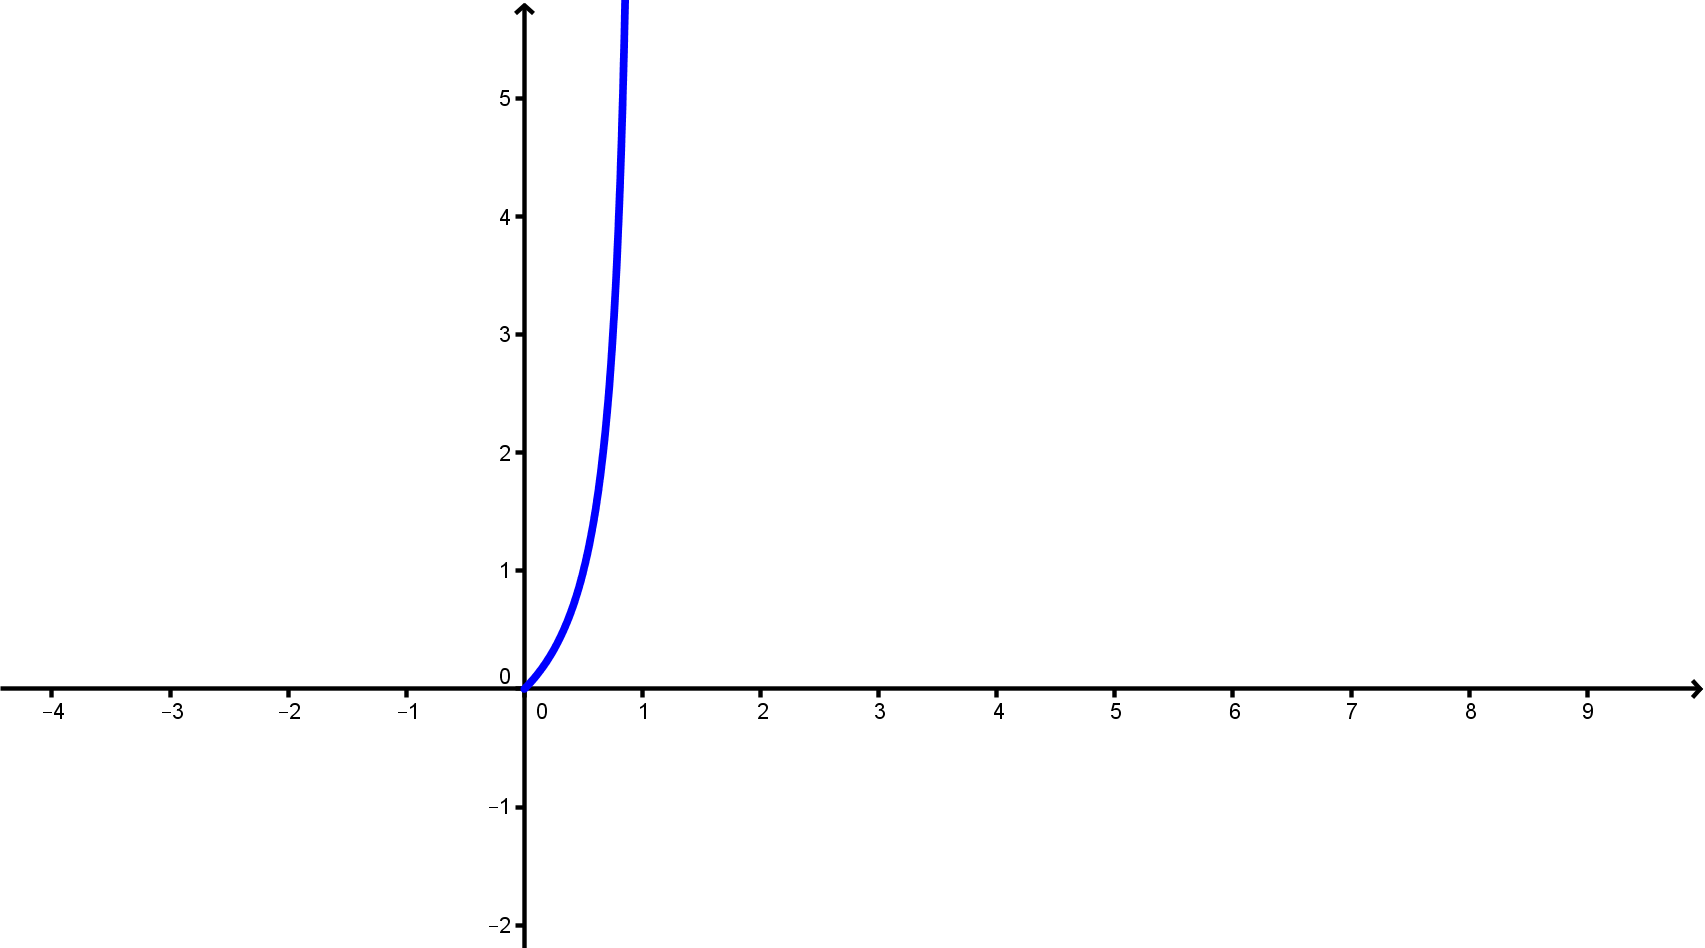
\includegraphics[width=10cm]{../fig/Cap03-OddsVsProbabilidad.png}
\end{enColor}
\begin{bn}
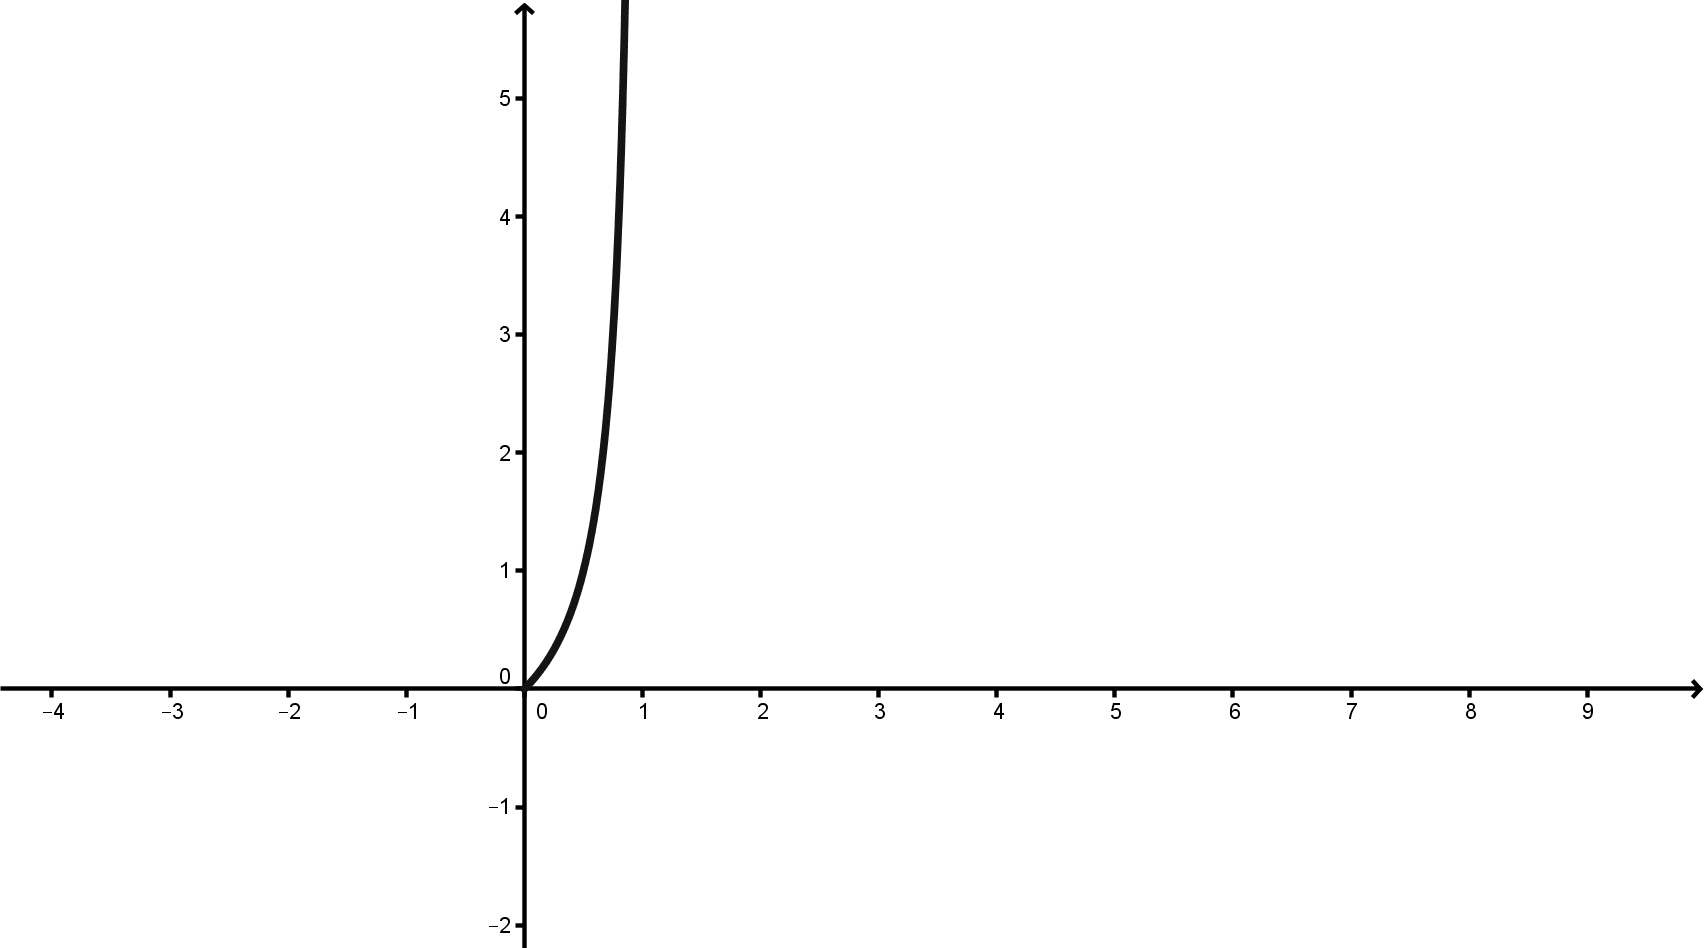
\includegraphics[width=10cm]{../fig/Cap03-OddsVsProbabilidad-bn.png}
\end{bn}
  \caption{Relación entre probabilidad (en el eje horizontal) y posibilidades (odds, en el eje vertical).}
  \label{cap12:Fig:OddsVsProbabilidad}
\end{center}
\end{figure}




\subsubsection*{Y entonces, ¿cómo funcionan las apuestas?}

Aunque no lo necesitamos estrictamente para nuestro trabajo, vamos a aprovechar para explicar el mecanismo de las {\sf apuestas basadas en posibilidades (odds)}\index{apuestas}.  La complicación adicional, en este caso, es que los apostadores a menudo utilizan las {\em posibilidades en contra} a la hora  de describir una apuesta.

Para fijar ideas, vamos a suponer que las apuestas están $7$ a $1$, {\em en contra de $A$}. En términos de posibilidades, eso significa:
\[
O_{A^c}=
\dfrac{\mbox{núm. de sucesos elementales favorables a $A^c$}}
{\mbox{núm. de sucesos elementales {\bf contrarios} a $A^c$}}=\dfrac{7}{1}.
\]
o, lo que es lo mismo,
\[
O_{A}=
\dfrac{\mbox{núm. de sucesos elementales {\bf contrarios} a $A$}}
{\mbox{núm. de sucesos elementales favorables a $A$}}
=\dfrac{1}{7}.
\]
Como puede deducirse, los apostadores creen que es siete veces más probable que ocurra $A^c$, frente a $A$. La apuesta por $A$, al ser más arriesgada, tiene un premio mucho mayor que la apuesta por $A^c$, que es la favorita de los apostadores. Una vez entendidas esas ideas, veamos cuales son las reglas que rigen las apuestas. Seguiremos con este ejemplo numérico para mayor claridad, y suponemos que las apuestas están $7$ a $1$ {\em en contra} de $A$:
\begin{itemize}
  \item Si yo apuesto por $A$, y ocurre $A$, eso quiere decir que, por cada euro que yo apuesto, me pagarán $7$ euros adicionales (además del que yo puse inicialmente). Naturalmente, si yo he apostado por $A$, y ocurre $A^c$, entonces pierdo el euro que aposté.
  \item  ¿Qué sucede si apuesto por $A^c$, cuando las apuestas están $7$ a $1$ {\em en contra} de  $A$? En este caso, en el que estoy apostando por el favorito, mis ganancias son el euro inicial, más $\frac{1}{7}$ de euro. Si apuesto por $A^c$, y gana $A$, de nuevo pierdo mi apuesta.
\end{itemize}
Para entender el razonamiento que hay detrás de estas reglas, tenemos que esperar hasta el Capítulo \ref{cap:VariablesAleatorias}, en el que, en la Sección \ref{cap04:subsec:VarianzaDesvTipicaVariableAleatoriaDiscreta} (pág. \pageref{cap04:subsec:VarianzaDesvTipicaVariableAleatoriaDiscreta}), introduciremos la idea de {\em juego justo}. Pero podemos ir adelantando algo del trabajo en un ejemplo:
\begin{ejemplo}
\label{cap03:ejem:OddsReglasApuestas}
Un corredor de apuestas sabe que siete apostadores quieren apostar, cada uno, un euro contra $A$, mientras que sólo un apostador está dispuesto a apostar un euro a favor de $A$. El apostador fija las apuestas $7$ a $1$ contra $A$, y reúne el dinero de los apostadores, que hace un total de $8$ euros.

Supongamos que ocurre $A^c$. Entonces el corredor de apuestas devuelve, a cada uno de los siete jugadores que apostaron contra $A$ el euro que apostaron, y usa el euro que se apostó a favor de $A$ para darles a esos jugadores un premio de $1/7$ de euro. El jugador que apostó a favor de $A$, naturalmente, ha perdido su euro.

Supongamos que ocurre $A$. Entonces el corredor de apuestas entrega, al único jugador que apostó por $A$, la totalidad de los ocho euros: su euro adicional, y los siete de los otros jugadores como premio. Los siete jugadores que apostaron contra $A$, naturalmente, han perdido su dinero.

En cualquier caso, el corredor de apuestas no pierde ni gana dinero, así que para él es básicamente indiferente quien gane o pierda. Naturalmente, los corredores de apuestas del mundo real quieren ganarse la vida con su negocio, así que las posibilidades (odds) que comunican a los jugadores tienen que incluir un cierto {\em sesgo} a su favor, para que ellos obtengan algún beneficio.
\qed
\end{ejemplo}
Con esto, ya estamos listos para dejar el garito de los apostadores, y volver a las pruebas diagnósticas.

%\subsubsection*{Posibilidades (odds) vs. probabilidades.}
%
%Si decimos que $O_A=7$, ¿cuál es nuestra estimación de la probabilidad de que $A$ gane? La idea es que $O_A=7$ significa que $B$ se considera $7$ veces más probable que $A$.  Y esto es lo que nos permite relacionar ambos conceptos. Si llamamos, como siempre, $P(A)$ y $P(B)$, a las probabilidades de $A$ y $B$ respectivamente, decir que $O_A=7$ significa que:
%\[P(B)=7\cdot P(A).\]
%Por otra parte, estamos suponiendo que $B=A^c$, de modo que
%\[1=P(A)+P(B),\]
%y por lo tanto:
%\[1=P(A)+7\cdot P(A)=8\cdot P(A).\]
%Es decir,
%\[P(A)=\dfrac{1}{8}.\]
%Repitiendo este razonamiento en general, se obtiene:
%\[P(A)=\dfrac{1}{1+O_A},\]
%y de aquí obtenemos la definición general.
%    \begin{center}
%    \fcolorbox{black}{Gris025}{
%    \begin{minipage}{12cm}
%    \begin{center}
%    {\bf Posibilidades (odds) de un suceso.}
%    \end{center}
%    Sea $A$ un suceso. Cuando decimos que el número $O_A$ representa las posibilidades a favor ({\em odds in favor}) del suceso $A$, eso equivale a decir que
%    \begin{equation}\label{cap03:ecu:OddsVsProbabilidades}
%    P(A)=\dfrac{1}{1+O_A}.
%    \end{equation}
%    Recíprocamente, dada la probabilidad $P(A)$, las posibilidades a favor de $A$ son:
%    \begin{equation}\label{cap03:ecu:ProbabilidadesVsOdds}
%    O_A=\dfrac{1}{P(A)}-1=\dfrac{1-P(A)}{P(A)}=\dfrac{P(A^c)}{P(A)}.
%    \end{equation}
%    \end{minipage}}
%    \end{center}
%
%Si decimos que
%
%
%La clave es entender la idea de {\em media o valor esperado}. En principio, una apuesta sólo se puede ganar o perder. Por lo tanto, se basa en una variable aleatoria de tipo Bernouilli (llamémosla $A$), con probabilidad $p$ de perder (de que yo pierda el dinero que he apostado) y $q=1-p$ de ganar. Supongamos que las proporciones para esta apuesta son de $k$ euros a 1. Es decir, si gano recibo $k$ euros por cada euro apostado (mientras que si pierdo, pierdo el euro que aposté, naturalmente). ¿Cuál es entonces el valor medio, o valor esperado de $A$? Pues sería
%\[\mu_A=q\cdot k+p\cdot(-1)\]
%El valor $-1$ en el segundo sumando corresponde a mis pérdidas (1 euro), si la suerte no me favorece.
%
%Dado este cálculo, ¿cuándo estamos ante una apuesta justa? Pues cuando mis ganancias esperadas son de cero euros (es decir, ni pierdo ni gano). Una apuesta justa debe cumplir:
%\[\mu_A=0\]
%Despejando de aquí, obtenemos una receta para calcular el valor $k$ que debería pagarnos el corredor de apuestas, una vez conocida la probabilidad $p$ de que yo gane la apuesta. En efecto, de
%\[0=q\cdot k+p\cdot(-1)\]
%se deduce
%\[
%k=\dfrac{p}{q}=\dfrac{p}{1-p}
%\]
%Esta relación entre proporciones (la cantidad $k$) y probabilidades no es del todo evidente. Por ejemplo, si la probabilidad de que yo pierda es del $80\%$ (es decir, $p=0.8$ y $q=0.2$) entonces, cuando gano, el corredor de apuestas debería pagarme
%\[
%k=\dfrac{0.8}{0.2}=4.
%\]
%euros por cada euro. Es una apuesta 4 a 1 si ha de ser justa. ¿Cuál debería ser el valor de $p$ para que la apuesta sea 10 a 1 (Calcúlalo; pero atención, {\sf no es el 90\%})?
%
%
%¿Qué tiene que ver toda esta terminología de apuestas con las pruebas diagnósticas? Supongo que el origen de todo es el hecho de que muchas personas (pacientes y/o personal sanitario) tienen problemas para entender el concepto de probabilidad. En cambio, la noción de proporciones (odds) en una apuesta es más conocida y familiar, para muchas de esas personas.
%
%La propia noción de prevalencia de una enfermedad se puede expresar, para ayudar a visualizarla, en términos de odds. Por ejemplo, si decimos que hay un enfermo de diabetes por cada 20 individuos sanos, {\bf no} estamos diciendo que la probabilidad sea
%\[\dfrac{1}{20}.\]
%Este número no es la probabilidad (prevalencia), sino la proporción. La prevalencia, es decir, la probabilidad, de hecho es (ahora debería ser evidente):
%\[\dfrac{1}{21}.\]
%Como vemos, la noción de odds o proporciones es simplemente otra forma de expresar la relación entre el número de enfermos y el total de la población.

\subsubsection*{Posibilidades (odds) pre y post diagnóstico.}

Una vez entendida la idea de posibilidades (odds), y para ver un ejemplo de su utilidad, vamos a aplicarla a las pruebas diagnósticas.  Como antes, llamamos $D$ al suceso {\em ``padecer la enfermedad''}, e indicaremos con los símbolos $+$ y $-$, los sucesos {\em ``prueba positiva''} y {\em ``prueba negativa''}, respectivamente.

Antes de realizar una prueba diagnóstica, ¿cuáles son las posibilidades (odds) de que el individuo esté enfermo? Es decir, las posibilidades a favor del suceso $D$. Usando la Ecuación \ref{cap03:ecu:OddsEnFuncionProbabilidades} (pág. \pageref{cap03:ecu:OddsEnFuncionProbabilidades}), se tiene:
\[\mbox{Posibilidades $D$ pre-prueba}=O_D=\dfrac{P(D)}{1-P(D)}\]
En inglés esta cantidad se describe como {\em pre-test odds}.

¿Y si ya hemos hecho la prueba, y el resultado ha sido positivo? ¿Cuánto valen ahora las posibilidades de $D$? Después de la prueba positiva, los valores relevantes son $P(D|+)$ y $P(D^c|+)$ (observa que estos dos valores también suman 1). Así que las probabilidades post-prueba (en inglés, {\em post-test odds})  pasan a ser:
\[\mbox{Posibilidades $D$ post-prueba}= \dfrac{P(D|+)}{P(D^c|+)}=\dfrac{P(D|+)}{1-P(D|+)}.\]
Lo que hace interesante estas expresiones es que las posibilidades pre y post prueba diagnóstica se pueden relacionar de forma muy sencilla con la razón de verosimilitud positiva $RVP$ de la Ecuación \ref{cap03:ecu:RazonVerosimilitudPositiva} (ver pág.\pageref{cap03:ecu:RazonVerosimilitudPositiva}; usamos $RVP$ porque la prueba ha sido positiva; si fuera negativa usaríamos $RVN$). Aquí es donde entra en acción el Teorema de Bayes. Por un lado, ese teorema nos dice que:
\[
P(D|+)=\dfrac{P(+|D)P(D)}{P(+|D)P(D)+P(+|D^c)P(D^c)}
\]
Y otra aplicación del teorema produce:
\[
P(D^c|+)=\dfrac{P(+|D^c)P(D^c)}{P(+|D^c)P(D^c)+P(+|D)P(D)}
\]
Ahora hay que darse cuenta de que, aunque el orden es distinto, los denominadores son iguales. Dividiendo las dos fracciones esos denominadores se cancelan y obtenemos, tras reorganizar un poco el resultado:
\[
\dfrac{P(D|+)}{P(D^c|+)}=\dfrac{P(+|D)}{P(+|D^c)}\cdot\dfrac{P(D)}{P(D^c)}.
\]
Teniendo en cuenta la terminología que hemos ido introduciendo, esto significa que (usamos odds en lugar de posibilidades para abreviar):
\begin{equation}\label{cap03:ecu:RelacionBayesianaOddsPrePostTestPositivo}
\left(\mbox{Odds $D$ post-prueba positiva}\right)=RVP\cdot \left(\mbox{Odds $D$ pre-prueba}\right).
\end{equation}
donde $RVP$ es, recordemos la Ecuación \ref{cap03:ecu:RazonVerosimilitudPositiva}, la razón de verosimilitud positiva de la prueba. Por un razonamiento análogo, se obtiene:
\begin{equation}\label{cap03:ecu:RelacionBayesianaOddsPrePostTestNegativo}
\left(\mbox{Odds $D$ post-prueba negativa}\right)=RVN\cdot \left(\mbox{Odds $D$ pre-prueba}\right).
\end{equation}
La Ecuación \ref{cap03:ecu:RelacionBayesianaOddsPrePostTestPositivo} permite, de una manera muy sencilla, actualizar nuestro cálculo de las posibilidades a favor de $D$, una vez obtenido un resultado positivo en la prueba. La relación entre ambas posibilidades es el factor $RVP$, la razón de verosimilitud positiva, que a su vez depende de la sensibilidad y la especificidad de la prueba.

\subsubsection{¿Qué es mejor, usar probabilidades o posibilidades (odds)?}
\label{cap03:subsubsec:QueEsMejorPosibilidadesProabilidades}

Ahora que ya sabemos qué son, y cómo se comportan las posibilidades, es posible que el lector se esté planteando la pregunta que encabeza este apartado. Y la mejor respuesta que podemos darle es que no hay una respuesta. Los dos objetos, posibilidades y probabilidades, son descripciones alternativas de una misma situación. Y tienen propiedades matemáticas distintas. Una probabilidad está obligada a permanecer en el intervalo $[0,1]$, y es muy fácil de convertir en un porcentaje. Por su parte, las posibilidades pueden tomar cualquier valor positivo (o infinito, si la probabilidad es $1$). Todavía no hemos avanzado suficiente en el curso para saber porque a veces es preferible que suceda una de esas dos cosas. Pero la buena noticia es, sin duda, que no hay ninguna necesidad de elegir. Las probabilidades y las posibilidades son herramientas de las que disponemos. Es como si tuviéramos que elegir si es mejor un destornillador o una llave inglesa. Lo mejor, sin duda, es llevar las dos en la caja de herramientas, y usar la herramienta adecuada para cada problema.

\subsubsection{Verosimilitud}
\label{cap03:subsubsec:verosimilitud}

La idea de {\sf verosimilitud}\index{verosimilitud} (en inglés, {\em likelihood}\index{likelihood}) es una idea muy importante en Estadística. Ya la hemos usado en el nombre de $RVP$ y en las ecuaciones como \ref{cap03:ecu:RelacionBayesianaOddsPrePostTestPositivo} y \ref{cap03:ecu:RelacionBayesianaOddsPrePostTestNegativo}.  A lo largo del curso nos la vamos a encontrar varias veces, e iremos añadiendo detalles a nuestra comprensión del concepto. Por el momento, aprovechando nuestro contacto con el Teorema de Bayes, nos vamos a conformar con una idea muy general.

El método científico se basa, muy esquemáticamente, en observar la naturaleza, formular teorías y modelos sobre ella, y contrastar esas teorías con los datos empíricos. Naturalmente, puesto que las teorías son explicaciones {\em parciales} de la realidad, sus predicciones no son nunca absolutamente exactas. Siempre se incluye un cierto margen de error, un {\em ruido} o componente aleatoria más o menos pequeño. Obviamente, para que la teoría sirva de algo, ese error o ruido tiene que ser pequeño, comparado con las cantidades que intervienen. En ese sentido, nunca esperamos de los científicos una certidumbre absoluta (hay otras instancias que se encargan de ese negocio...). No, lo que se espera de una teoría científica es un {\em control adecuado del error}, entendido como un procedimiento para medir la magnitud de ese error. Usando el lenguaje de la probabilidad condicionada, podemos expresar así ese control:
\[P\left(\mbox{datos}\,|\,\mbox{teoría cierta}\right).\]
Es decir, la teoría tiene que ser capaz de responder a preguntas como: {\em ``si la teoría es cierta, ¿cuál es la probabilidad de observar ciertos datos concretos?''} Un ejemplo sencillo puede ayudar a entender esto: supongamos que mi teoría dice que el dado no está cargado (todos los valores son equiprobables). Entonces, puedo usar esa teoría para predecir, por ejemplo (y usando la Regla de Laplace)
\[P\left(\mbox{resultado = }5\,|\,\mbox{teoría = ``dado no cargado''}\right)=\dfrac{1}{6}.\]
El otro componente esencial del método científico es la comparación de la teoría con los datos. Si, después de lanzar $1000$ veces el dado, el $5$ sólo hubiera aparecido $10$ veces, mi teoría de que el dado no está cargado se vería en un serio aprieto. En esta parte del trabajo, la pregunta que nos interesa tiene más que ver con la probabilidad condicionada recíproca de la anterior:
\[P\left(\mbox{teoría cierta}\,|\,\mbox{datos}\right).\]
Piénsalo así: dados los datos ($1000$ lanzamientos en los que el $5$ sólo aparece $10$ veces), ¿cuál es la probabilidad de que la teoría (``el dado no está cargado'') sea cierta? Ese valor no es $0$, desde luego. Pero es un valor tan ridículamente pequeño, que nadie en sus cabales seguiría creyendo en la teoría después de observar esos datos. Para describir lo que esperamos de la Ciencia, nos viene a la mente esa frase frecuente en el sistema judicial anglosajón: ``más allá de cualquier duda razonable'' (en inglés {\em ``beyond a reasonable doubt''}).

La relación entre las dos probabilidades condicionadas anteriores, viene determinada por el Teorema de Bayes:
\[
P(\mbox{teoría cierta}|\mbox{datos})=
\dfrac{
P(\mbox{datos}|\mbox{teoría cierta})\cdot P(\mbox{teoría cierta})}{P(\mbox{datos})}.
\]
que se puede expresar así:
\begin{equation}
\label{cap03:ecu:FuncionVerosimilitudBayes}
\underbrace{
P(\mbox{teoría cierta}|\mbox{datos})}_{\mbox{\tiny después de los datos}}=
\dfrac{\mathcal{L}(\mbox{datos, teoría cierta})}{P(\mbox{datos})}
\cdot
\underbrace{
P(\mbox{teoría cierta})}_{\mbox{\tiny antes de los datos}}
,\end{equation}
donde $\mathcal{L}(\mbox{datos, teoría cierta})=P(\mbox{datos}|\mbox{teoría cierta})$ es la {\sf función verosimilitud}\index{función verosimilitud}\index{verosimilitud, función}. Como hemos indicado, el término $P(\mbox{teoría cierta})$ indica nuestro grado de creencia en la teoría antes de ver los datos. Y el término de la izquierda, $P(\mbox{teoría cierta}|\mbox{datos})$ nos dice cómo ha cambiado esa creencia una vez examinados los datos. El cociente que los relaciona es un {\em artefacto estadístico}, es la forma en la que la Estadística nos ayuda a actualizar nuestras creencias sobre esa teoría. En particular, esa actualización pasa por comparar nuestra teoría con las posibles teorías alternativas. Por eso la teoría aparece como una variable de la función de verosimilitud, porque vamos a considerar distintas teorías. En próximos capítulos iremos conociendo esta función en más detalle.

La Ecuación \ref{cap03:ecu:FuncionVerosimilitudBayes} resume (de manera muy simplificada) el proceso por el que el método científico actualiza su confianza en una teoría. Podemos verlo de esta manera: tenemos una teoría que deseamos someter a escrutinio, y acabamos de obtener una colección de datos. A la izquierda, de la Ecuación \ref{cap03:ecu:FuncionVerosimilitudBayes} está la pregunta a la que queremos responder: ``¿qué probabilidad hay de que esa teoría sea cierta, a la luz de estos datos?'' La respuesta, tal como nos la proporciona el lado derecho de la Ecuación \ref{cap03:ecu:FuncionVerosimilitudBayes}, tiene tres ingredientes:
\begin{itemize}
  \item $P(\mbox{teoría cierta})$, es una medida de nuestra confianza en esa teoría {\em previa} a la aparición de esos datos. A menudo se dice que es la probabilidad {``a priori''}\index{a priori} (en inglés {\em prior probability}) o, simplemente, {\em prior}.
  \item $\mathcal{L}(\mbox{datos, teoría cierta})$ es el valor de la función verosimilitud, cuando la teoría es cierta. Podríamos decir que aquí es donde entra en juego la Estadística, que nos tiene que decir cual es esa función.
  \item La probabilidad $P(\mbox{datos})$ representa la probabilidad (absoluta, no condicionada) de los datos, y es la parte menos accesible para nosotros de esta expresión.
\end{itemize}
Precisamente por esta última observación, la función de verosimilitud se lleva especialmente bien con la idea de posibilidades (odds).  Si escribimos la ecuación análoga a \ref{cap03:ecu:FuncionVerosimilitudBayes} para el cálculo de la probabilidad de que la teoría sea falsa (con los mismos datos), tenemos:
\[
P(\mbox{teoría falsa}|\mbox{datos})=
\dfrac{\mathcal{L}(\mbox{datos, teoría cierta})}{P(\mbox{datos})}
\cdot P(\mbox{teoría falsa})
\]
Y si dividimos la Ecuación \ref{cap03:ecu:FuncionVerosimilitudBayes} por esta ecuación tenemos:
\begin{equation}
\label{cap03:ecu:CocienteVerosimilitudes}
%O(\mbox{teoría falsa}|\mbox{datos})=
\dfrac{P(\mbox{teoría cierta}|\mbox{datos})}{P(\mbox{teoría falsa}|\mbox{datos})}=
\dfrac{\mathcal{L}(\mbox{datos, teoría cierta})}{\mathcal{L}(\mbox{datos, teoría falsa})}
\cdot
\dfrac{P(\mbox{teoría cierta})}{P(\mbox{teoría falsa})}.
\end{equation}
El último término de la derecha de esta ecuación son las posibilidades a favor de que la teoría sea cierta {\em a priori}. Vienen a representar nuestra confianza en esa teoría antes de conocer los datos. Para ver esto, sólo hay que tener en cuenta que {\em teoría cierta} y {\em teoría falsa} son complementarios, y recordar la definición \ref{cap03:ecu:ProbabilidadesEnFuncionOdds} (pág. \pageref{cap03:ecu:ProbabilidadesEnFuncionOdds}). De la misma forma, el término de la izquierda son las posibilidades (odds) a favor de que la teoría sea cierta, {\em a posteriori}; es decir, una vez que tenemos en cuenta los datos. Y como se ve, el mecanismo para actualizar nuestra visión de la validez de esa teoría es el {\sf cociente o razón de verosimilitudes}\index{cociente de verosimilitudes}\index{verosimilitudes, cociente o razón} (en inglés {\em likelihood ratio}\index{likelihood ratio}). Fíjate, en particular, en que este enfoque elimina el término $P(\mbox{datos})$ que nos causaba problemas. Por tanto, podemos escribir así la Ecuación \ref{cap03:ecu:CocienteVerosimilitudes}:

\begin{equation}
\label{cap03:ecu:OddsCocienteVerosimilitudes}
%O(\mbox{teoría falsa}|\mbox{datos})=
O_{\mbox{teoría cierta}|\mbox{datos}}=
\dfrac{\mathcal{L}(\mbox{datos, teoría cierta})}{\mathcal{L}(\mbox{datos, teoría falsa})}
\cdot
O_{\mbox{teoría cierta}}
\end{equation}

Conviene, además, comparar esta Ecuación \ref{cap03:ecu:CocienteVerosimilitudes} con las Ecuaciones \ref{cap03:ecu:RelacionBayesianaOddsPrePostTestPositivo} y \ref{cap03:ecu:RelacionBayesianaOddsPrePostTestNegativo} (pág. \pageref{cap03:ecu:RelacionBayesianaOddsPrePostTestPositivo}), para ver que su estructura es la misma. Para hacer la analogía más completa, puedes pensar que en el caso de las pruebas diagnósticas la teoría es el suceso que hemos llamado $D =${\em ``el paciente está enfermo''}, mientras que los datos son el suceso que hemos llamado $+ = ${\em ``el diagnóstico es positivo''.}

Seguramente esta discusión tan genérica puede resultar un poco desconcertante, al menos la primera vez. Hasta cierto punto, es inevitable que así sea; por la novedad, y porque nuestra experiencia con la idea de verosimilitud, a estas alturas del curso, es mínima. En próximos capítulos volveremos sobre esa idea varias veces, y las cosas irán quedando cada vez más claras.

%\section{Ejercicios para practicar estas ideas}
%
%
%\begin{enumerate}
%
%    \item  En un estudio en el que se incluyen 1000 pacientes enfermos y 100 no enfermos, una prueba diagnostica clasifica como positivos al 70\% de los enfermos, y como negativos al 95\% de los no enfermos. Calcular la sensibilidad y la especificidad de la prueba.
%
%    \item  La sensibilidad de una prueba diagnóstica es $0.95$ y su especificidad es $0.85$. Si la prevalencia de la enfermedad es $0.002$, ¿cuál es el valor predictivo positivo del test?
%
%    \item En la información que describe un test de embarazo se puede leer ``Cuando los usuarios del test son mujeres que recogen y ensayan sus propias muestras, la sensibilidad del test es del 75\%. La especificidad también es baja, de entre un 52\% y un 75\%.'' Aceptando el valor más bajo para la especificidad, ¿cuánto vale la razón de verosimilitud diagnóstica negativa de este test? Vamos a suponer que una mujer ha obtenido un resultado negativo en el test. Sabiendo que un 30\% de las mujeres que realizan pruebas de embarazo están de hecho embarazadas, ¿cuál es la probabilidad de que esta mujer lo esté?
%
%    \item Un estudio que compara la eficacia de varias pruebas diagnósticas del VIH describe un experimento en el que se obtuvo que los test de anticuerpos del VIH tienen una sensibilidad del 99.7\% y una especificidad del 98.5\%. Supongamos queun individuo, dentro de una población con una prevalencia del 0.1\%  de VIH, obtiene un resultado positivo en uno de estos test de anticuerpos. ¿Cuál es la probabilidad de que realmente tenga el VIH? ¿Cuál es el valor predictivo positivo de este test?
%
%    \item La siguiente tabla muestra los resultados de un test de diagnóstico que se utilizó con dos muestras independientes de 650 sujetos enfermos y 1200 sujetos sanos.
%
%        \begin{center}
%            \begin{tabular}{llccc}
%            &&\multicolumn{3}{c}{\underline{\bf Estado real}}\\
%
%                                  &          & Enfermos & Sanos& \\
%            \hline
%  \underline{\bf Resultado del test}          & Positivo & 490 & 70   &   \\
%                                              & Negativo & 160 & 1130 &   \\
%            \hline
%                                              &          &     &     &    \\
%            \hline
%            \end{tabular}
%        \end{center}
%        Calcular la sensibilidad y la especificidad del test. Si la prevalencia de la enfermedad es $0.002$, ¿cuál es el valor predictivo positivo del test?
%
%
%    \item Los resultados de la siguiente tabla se obtuvieron en un estudio diseñado para averiguar la capacidad de un cirujano anatomopatólogo para clasificar correctamente biopsias quirúrgicas en malignas o benignas. Aproximar $\alpha$ y $\beta$ a partir de estos datos.
%
%        \begin{center}
%            \begin{tabular}{llccc}
%            &&\multicolumn{3}{c}{\underline{\bf Estado real}}\\
%
%                                  &          & Benigno (-)& Maligno (+)& Total\\
%            \hline
%  \underline{\bf Informe del anatomopatólogo} & Positivo & 7 & 79   &   \\
%                                              & Negativo & 395  & 19 &   \\
%            \hline
%                                              &          &     &     & 500  \\
%            \hline
%            \end{tabular}
%        \end{center}
%
%    \item Se está ensayando un nuevo método para detectar enfermedades renales en pacientes con hipertensión. Se aplica el nuevo procedimiento a 137 pacientes hipertensos. Y a continuación, a esos mismos pacientes se les aplica un método anterior, bien contrastado, para comprobar la presencia o ausencia de enfermedad renal. Los datos obtenidos se recogen en la tabla. Utilizando estos datos, calcular aproximadamente la probabilidad de falso positivo y la de falso negativo del nuevo método. Aproximar asimismo el valor predictivo positivo y el valor predictivo negativo del nuevo método.
%
%        \begin{center}
%            \begin{tabular}{llccc}
%            &&\multicolumn{3}{c}{\underline{\bf Estado real (método clásico)}}\\
%
%                                  &          & Sano (-)& Enfermo (+)& Total\\
%            \hline
%            \underline{\bf Nuevo método}     & Enfermo (+) & 23  & 44 &   \\
%                                             & Sano (-) & 60  & 10 &   \\
%            \hline
%                                              &          &     &     & 137  \\
%            \hline
%            \end{tabular}
%        \end{center}
%
%\item En la siguiente tabla se muestran los resultados de un estudio para evaluar la utilidad de una tira reactiva para el diagnóstico de infección urinaria.
%        \begin{center}
%            \begin{tabular}{llccc}
%            &&\multicolumn{3}{c}{\underline{\bf Estado real}}\\
%
%                                  &          & Con infección& Sin infección&\\
%            \hline
%            \underline{\bf Tira reactiva}     & Positivo & 60  & 80 &   \\
%                                             & Negativo & 10  & 200 &   \\
%            \hline
%                                              &          &     &     & 350  \\
%            \hline
%            \end{tabular}
%        \end{center}
%        Calcular e interpretar sensibilidad y especificidad, y los valores predictivos positivo y negativo. Si conocemos que la prevalencia de la infección en la población de interés es del 2\%, ¿cómo se verían afectados los valores predictivos? ¿Es esta tira reactiva una buena prueba diagnóstica?
%
%\end{enumerate}


\chapter{Variables aleatorias.}
\label{cap:VariablesAleatorias}
% !Mode:: "Tex:UTF-8"

\section{Variables aleatorias.}\label{sec:variablesAletorias}

\subsection{¿Qué son las variables aleatorias?}
\label{Cap04:subsec:QueSonVariablesAleatorias}

Hemos visto que cada suceso $A$ del espacio muestral $\Omega$ tiene asociado un valor $P(A)$ de la función probabilidad. Y sabemos que los valores de la función probabilidad son valores positivos, comprendidos entre $0$ y $1$. La idea de variable aleatoria es similar, pero generaliza este concepto, porque a menudo querremos asociar otros valores numéricos con los resultados de un experimento aleatorio.
\begin{Ejemplo}
\label{cap04:ejem:VariableAleatoriaSumaDosDados}
    Quizá uno de los ejemplos más sencillos sea lo que ocurre cuando lanzamos dos dados, y nos fijamos en la suma de los valores obtenidos. Esa suma es siempre un número del 2 al 12, y es perfectamente legítimo hacer preguntas como ¿cuál es la probabilidad de que  la suma valga $7$? Para responder a esa pregunta, iríamos al espacio muestral (formado por 36 resultados posibles), veríamos el valor de la suma en cada uno de ellos, para localizar aquellos en que la suma vale $7$. Así obtendríamos un suceso aleatorio $A=\{(1,6),(2,5),(3,4),(4,3),(5,2),(6,1)\}$, cuya probabilidad es $6/36$. De hecho podemos
    repetir lo mismo para cada uno de los posibles valores de la suma. Se obtiene la Tabla \ref{cap04:tabla:probabilidadSumaDados}, que vamos a llamar la {\sf tabla de densidad} de probabilidad de la variable suma.\qed
    \begin{table}[ht]
    \begin{center}
    {\small
    \begin{tabular}[t]{|c|c|c|c|c|c|c|c|c|c|c|c|}
    \hline
    \begin{minipage}{2cm}
    \rule{0cm}{0.7cm}{\em Valor de\\ la suma:\\[2mm]}
    \end{minipage}
    &2&3&4&5&6&7&8&9&10&11&12\\
    \hline
    \begin{minipage}{2cm}
    \rule{0cm}{1cm}{\em Probabilidad\\
    de ese valor:}
    \end{minipage}
    &$\dfrac{1}{36}$&$\dfrac{2}{36}$&$\dfrac{3}{36}$&$\dfrac{4}{36}$&$\dfrac{5}{36}$&$\dfrac{6}{36}$&$\dfrac{5}{36}$&$\dfrac{4}{36}$&$\dfrac{3}{36}$&$\dfrac{2}{36}$&$\dfrac{1}{36}$\\
    &&&&&&&&&&&\\
    \hline
    \end{tabular}
    }
    \caption{Tabla de densidad de probabilidad de las posibles sumas, al lanzar dos dados}
    \label{cap04:tabla:probabilidadSumaDados}
    \end{center}
    \end{table}
\end{Ejemplo}
Vamos ahora a ver otro ejemplo, en este caso inspirado en los problemas de probabilidad geométrica.
\begin{Ejemplo}\label{ejem:ProbabilidadGeometricaSubconjuntosCirculo}
    Consideremos un círculo $C$ centrado en el origen y de radio 1. El espacio muestral $\Omega$ está formado por todos los subconjuntos\footnote{Subconjuntos que no sean excesivamente ``raros'', en el sentido que ya hemos discutido.} de puntos de $C$. Y la probabilidad de un subconjunto $A$ se define así:
    \[P(A)=\mbox{área de }A.\]
    Consideremos ahora la variable $X(x,y)=x$, que a cada punto del círculo le asocia su coordenada $x$. En este caso la coordenada $x$ toma cualquier valor real entre $-1$ y $1$. Y si preguntamos {``¿cuál es la probabilidad de que tome por ejemplo el valor $1/2$?''}, la respuesta es $0$. Porque los puntos del círculo donde toma ese valor forman un segmento (una cuerda del círculo), y el segmento tiene área $0$. Las cosas cambian si preguntamos {``¿cuál es la probabilidad de que la coordenada $x$ esté entre $0$ y $1/2$?''} En este caso, como muestra la Figura \ref{cap04:fig:EjemploVariableAleatoriaContinua}
    \begin{figure}[h]
	\centering
	\begin{enColor}
    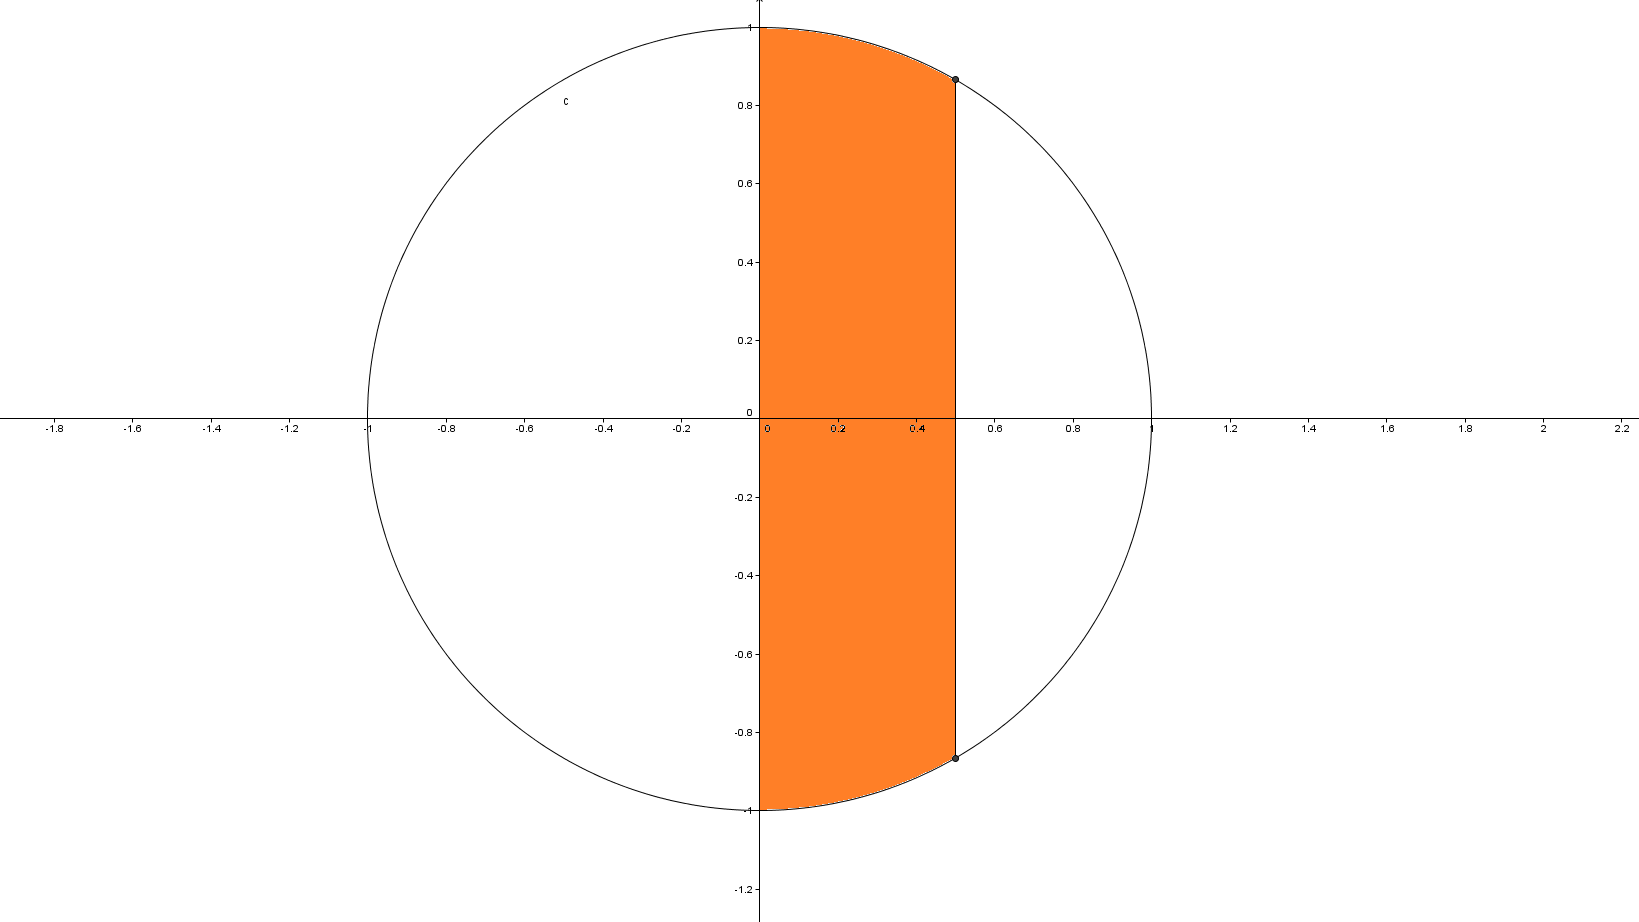
\includegraphics[height=7cm]{../fig/Cap04-Figura01-VariableAleatoriaContinua.png}
	\end{enColor}
	\begin{bn}
    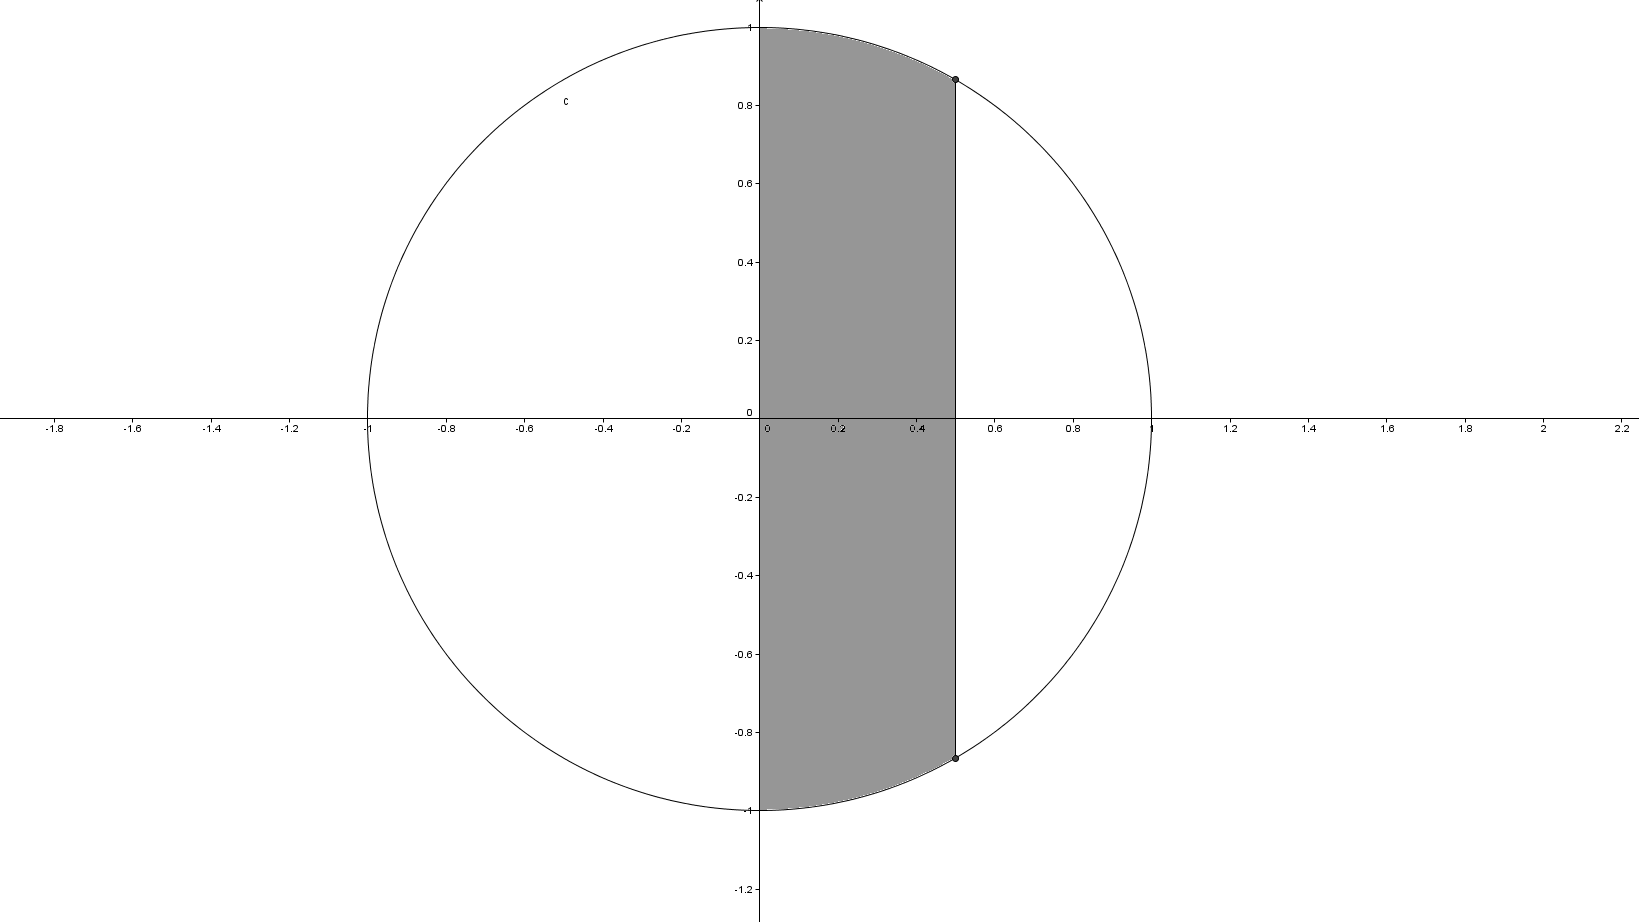
\includegraphics[height=7cm]{../fig/Cap04-Figura01-VariableAleatoriaContinua-bn.png}
	\end{bn}
	\caption{Cálculo de probabilidad en una variable aleatoria continua}
	\label{cap04:fig:EjemploVariableAleatoriaContinua}
    \end{figure}
el conjunto de puntos del círculo cuyas coordenadas $x$ están entre $0$ y $1/2$ tiene un área bien definida y no nula. ¿Cuánto vale ese área? Aproximadamente $0.48$, y esa es la probabilidad que buscábamos. El cálculo del área se puede hacer de distintas maneras, pero el lector debe darse cuenta de que en ejemplos como este se necesita a veces recurrir al cálculo de integrales.\\
    Naturalmente, se pueden hacer preguntas más complicadas. Por ejemplo, dado un punto $(x,y)$ del círculo $C$ podemos calcular el valor de $f(x,y)=x^2+ 4y^2$. Y entonces nos preguntamos ¿cuál es la probabilidad de que, tomando un punto al azar en $C$, el valor de $f$ esté entre 0 y 1? La respuesta es, de nuevo, un área, pero más complicada: es el área que se muestra en la Figura \ref{cap04:fig:EjemploVariableAleatoriaContinua2}.
    \begin{figure}[h]
	\centering
	\begin{enColor}
    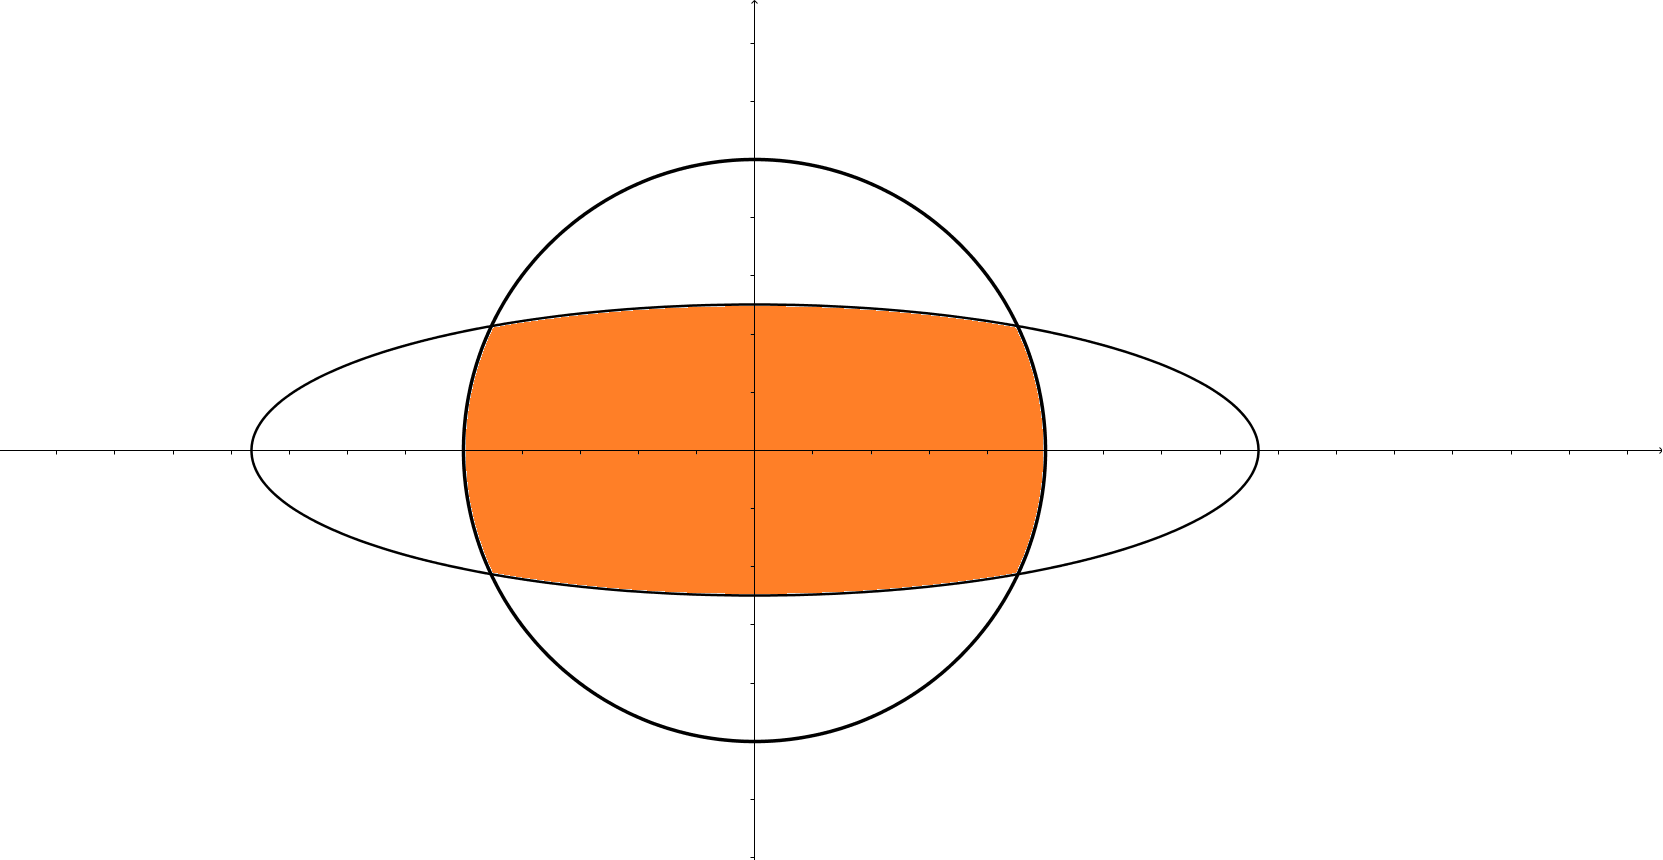
\includegraphics[height=7cm]{../fig/Cap04-Figura02-VariableAleatoriaContinua.png}
	\end{enColor}
	\begin{bn}
    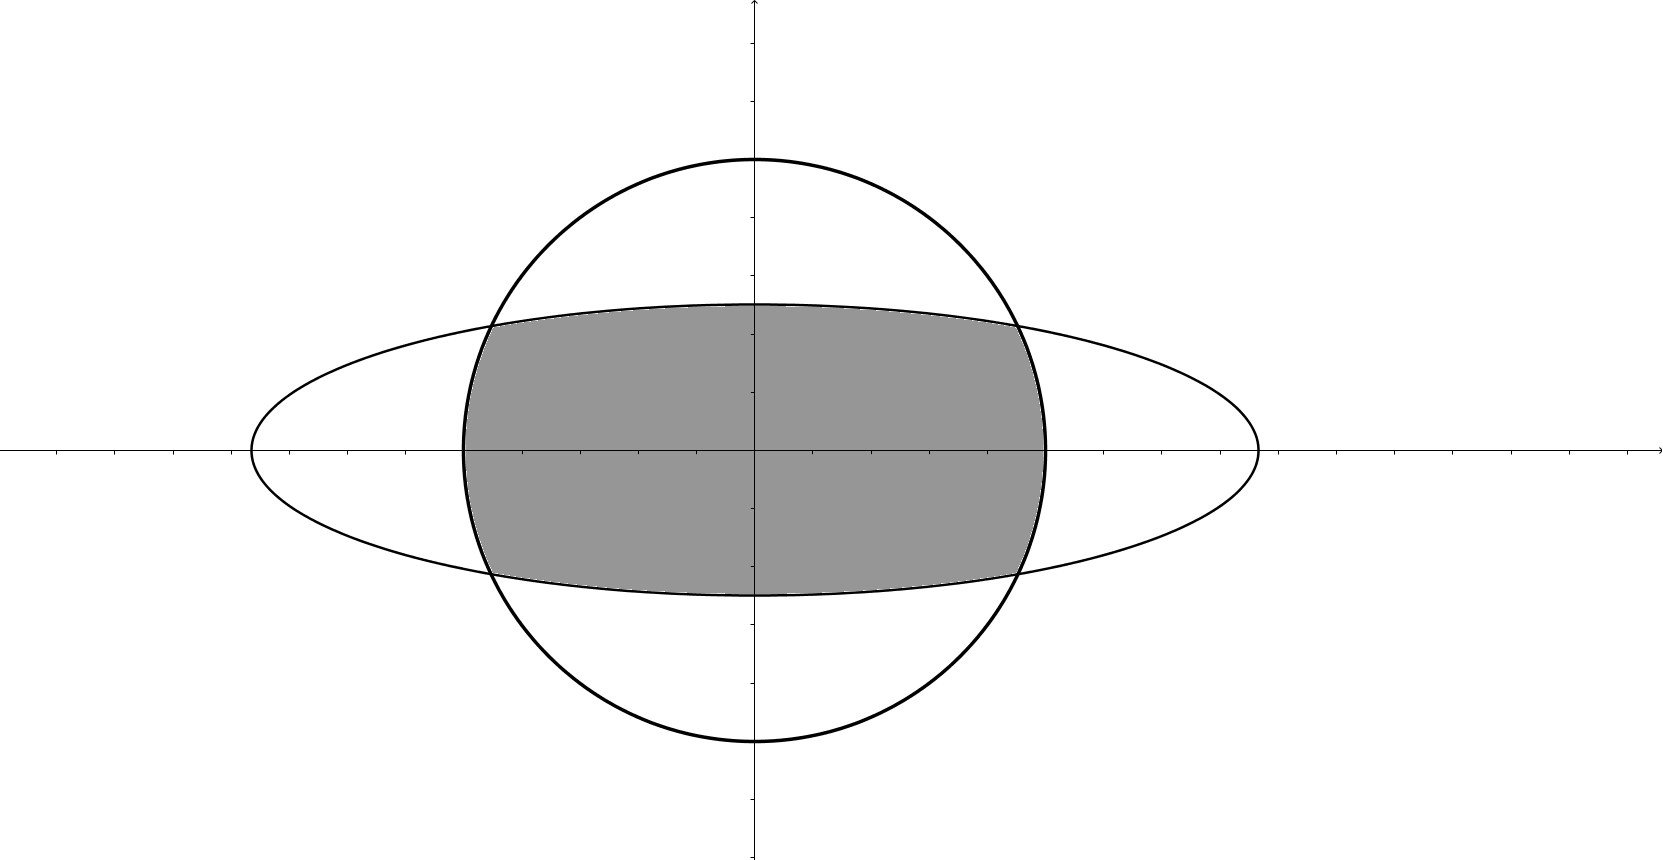
\includegraphics[height=7cm]{../fig/Cap04-Figura02-VariableAleatoriaContinua-bn.png}
	\end{bn}
	\caption{Un cálculo de probabilidad más complicado, para una variable aleatoria continua.}
	\label{cap04:fig:EjemploVariableAleatoriaContinua2}
    \end{figure}
    Lo que tienen en común ambos casos es que hay una función (o fórmula), que es $x$ en el primero y $f(x,y)$ en el segundo, y que nos preguntamos por la probabilidad de que los valores de esa fórmula caigan dentro de un cierto intervalo.
    \qed
\end{Ejemplo}
Los dos ejemplos que hemos visto contienen los ingredientes básicos de la noción de variable aleatoria. En el primer caso teníamos un conjunto finito de valores posibles, y a cada uno le asignábamos una probabilidad. En el segundo caso teníamos un recorrido continuo de valores posibles, y podíamos asignar probabilidades a intervalos. Lo que vamos a ver a continuación no se puede considerar de ninguna manera una definición rigurosa de variable aleatoria, pero servirá a nuestros propósitos.
    \begin{center}
    \fcolorbox{black}{Gris025}{
    \begin{minipage}{12cm}
        \begin{center}\bf Variables aleatorias:\end{center}
        Una {\sf variable aleatoria}\index{variable aleatoria} $X$ es una función (o fórmula) que le asigna, a cada elemento $p$ del espacio muestral $\Omega$, un número real $X(p)$. Distinguimos dos tipos de variables aleatorias:
        \begin{enumerate}
            \item La {\sf variable aleatoria $X$ es discreta}\index{variable aleatoria discreta} si sólo toma una cantidad finita (o una sucesión) de valores numéricos $x_1,x_2,x_3,\ldots$, de manera que para cada uno de esos valores tenemos bien definida la probabilidad $p_i=P(X=x_i)$ de que $X$ tome el valor $x_i$.
            \item La {\sf variable aleatoria $X$ es continua}\index{variable aleatoria continua} si sus valores forman un conjunto continuo dentro de los números reales (como una unión finita de intervalos, acotados o no), de manera que si nos dan un intervalo $I=(a,b)$ (aquí puede ser $a=-\infty$ o $b=+\infty$), tenemos bien definida la probabilidad $P(X\in I)$ de que el valor de $X$ esté dentro de ese intervalo $I$.
        \end{enumerate}
    \end{minipage}}
    \end{center}
¿Por qué no es una definición rigurosa? La situación es similar a lo que ocurría al definir los sucesos aleatorios. Un suceso aleatorio $A$ es un subconjunto que tiene bien definida la probabilidad $P(A)$. Pero, como ya hemos dicho, hay conjuntos tan {\em raros} que no es fácil asignarles un valor de la probabilidad, igual que a veces cuesta asignar un valor del área a algunas figuras muy raras. De la misma forma hay funciones tan raras que no se pueden considerar variables aleatorias. Se necesitan definiciones más rigurosas, pero que aquí sólo complicarían la discusión. Veamos un ejemplo, muy parecido al Ejemplo \ref{cap04:ejem:VariableAleatoriaSumaDosDados} (pág. \pageref{cap04:ejem:VariableAleatoriaSumaDosDados}).
\begin{Ejemplo}\label{ejem:VariableAleatoria:RestaDosDados}
    En el Ejemplo \ref{cap04:ejem:VariableAleatoriaSumaDosDados}, cada punto del espacio muestral es un par de números $(a,b)$, obtenidos al lanzar los dos dados. Podemos entonces definir una variable aleatoria $X$, que a cada punto $(a,b)$ del espacio muestral, le asigna la suma de esos dos valores:
    \[X(a,b)=a+b.\]
    En este caso, los valores de la probabilidad asignados por esta variable $X$ son los de la Tabla \ref{cap04:tabla:probabilidadSumaDados}.


    Siguiendo con este mismo espacio muestral, del lanzamiento de dos dados, en lugar de la suma ahora nos fijamos en la diferencia absoluta de los valores obtenidos (el mayor menos el menor, y cero si son iguales). Si llamamos $(a,b)$ al resultado de lanzar los dados, donde $a$ y $b$ son números del 1 al 6, entonces estamos definiendo una variable aleatoria mediante la expresión
    \[Y(a,b)=|a-b|.\]
    Esta claro que la variable $Y$ toma solamente los valores $0,1,2,3,4,5$. ¿Cuál es la probabilidad de que al calcular $Y$ obtengamos $3$? El siguiente diagrama ayudará a entender la respuesta. Para cada punto del espacio muestral se muestra el valor de $Y$:
    \[
    \begin{array}{cccccc}
    Y(1,1)=0&Y(1,2)=1&Y(1,3)=2&Y(1,4)=3&Y(1,5)=4&Y(1,6)=5\\
    Y(2,1)=1&Y(2,2)=0&Y(2,3)=1&Y(2,4)=2&Y(2,5)=3&Y(2,6)=4\\
    Y(3,1)=2&Y(3,2)=1&Y(3,3)=0&Y(3,4)=1&Y(3,5)=2&Y(3,6)=3\\
    Y(4,1)=3&Y(4,2)=2&Y(4,3)=1&Y(4,4)=0&Y(4,5)=1&Y(4,6)=2\\
    Y(5,1)=4&Y(5,2)=3&Y(5,3)=2&Y(5,4)=1&Y(5,5)=0&Y(5,6)=1\\
    Y(6,1)=5&Y(6,2)=4&Y(6,3)=3&Y(6,4)=2&Y(6,5)=1&Y(6,6)=0
    \end{array}
    \]
    Y se observa que $P(Y=3)=6/36=1/6$. De hecho, podemos repetir lo mismo para cada uno de los posibles valores de la variable aleatoria $Y$. Se obtiene la tabla de densidad de probabilidad que aparece como Tabla \ref{cap04:tabla:VariableAleatoriaDiferencia2Dados}.
    %Y de nuevo, insistimos, esta tabla es lo que en este caso caracteriza a la variable aleatoria diferencia $Y$. Se puede decir, sin riesgo de confusión, que {\sf\em esta tabla es la variable aleatoria $Y$. De la misma forma, la Tabla \ref{cap04:tabla:probabilidadSumaDados} define a la variable suma $X$.}
    \begin{table}[ht]
    \begin{center}
    \begin{tabular}[t]{|c|c|c|c|c|c|c|}
    \hline
    \rule{0cm}{0.5cm}{\em Valor de $Y$ (diferencia):}&0&1&2&3&4&5\\
    \hline
    \rule{0cm}{0.7cm}{\em Probabilidad de ese valor:}&$\dfrac{6}{36}$&$\dfrac{10}{36}$&$\dfrac{8}{36}$&$\dfrac{6}{36}$&$\dfrac{4}{36}$&$\dfrac{2}{36}$\\
    &&&&&&\\
    \hline
    \end{tabular}
    \end{center}
    \caption{Variable aleatoria diferencia al lanzar dos dados}\label{cap04:tabla:VariableAleatoriaDiferencia2Dados}
    \end{table}
    \qed
\end{Ejemplo}


\subsection{Variables aleatorias y sucesos. Función de densidad.}
\label{cap04:subsec:VariablesAleatoriasSucesos}

Al principio la diferencia entre suceso aleatorio y variable aleatoria puede resultar un poco confusa. Vamos a recordar lo que es cada uno de estos conceptos:
\begin{enumerate}
    \item Un suceso es un {\em subconjunto}, mientras que una variable aleatoria es una {\em función}. Por ejemplo, al lanzar dos dados, un suceso puede ser ``los dos resultados son pares'', y en este enunciado no hay un valor numérico fácil de identificar. Lo que sí tenemos es una {\em probabilidad asociada a este suceso}.
    \item Por el contrario, al considerar la variable aleatoria $Y(a,b)=|a-b|$, definida en el espacio muestral de los 36 resultados posibles, al lanzar dos dados, el valor numérico está claramente definido: $|a-b|$. Pero la definición de la operación {``diferencia en valor absoluto de los dados''}, por si misma, no define ningún suceso.
\end{enumerate}
¿Cuál es entonces el origen de la confusión? Posiblemente, la parte más confusa es que {\sf\em las variables aleatorias definen sucesos cuando se les asigna un valor}. Por ejemplo, si escribimos $Y(a,b)=|a-b|=3$, estamos pensando en el suceso {\em ``la diferencia de los resultados de los dados es 3''}. Es decir, el suceso formado por
\[\{(1,4),(2,5),(3,6),(6,3,),(5,2),(4,1)\}.\]
Y hemos visto en el Ejemplo \ref{ejem:VariableAleatoria:RestaDosDados} que la probabilidad de ese suceso es
\[P(Y=3)=1/6.\]
¿Para qué sirven entonces las variables aleatorias? Simplificando podemos decir que son, entre otras cosas, un atajo para hacer más sencillo el trabajo con sucesos. Precisando un poco más, su utilidad es que representan {\sf modelos abstractos de asignación (o distribución) de probabilidad}. Es decir, la variable aleatoria nos permite concentrar nuestra atención en la forma en que la probabilidad se reparte o {\em distribuye} entre los posibles resultados numéricos de un experimento aleatorio, sin entrar en detalles sobre el espacio muestral y los sucesos subyacentes a esa asignación de probabilidad.  Vamos a ver un par de ejemplos que tal vez ayude a aclarar el sentido en el que estas variables aleatorias son resúmenes que eliminan detalles (y por tanto, a menudo, información).
\begin{Ejemplo}\label{cap04:ejem:VariablesAleatoriasEliminanInformacion}
    Ya hemos discutido que en el espacio muestral correspondiente al lanzamiento de dos dados, la variable aleatoria $Y(a,b)=|a-b|$ tiene la tabla de densidad de probabilidades que se muestra en la Tabla \ref{cap04:tabla:VariableAleatoriaDiferencia2Dados} (pág. \pageref{cap04:tabla:VariableAleatoriaDiferencia2Dados}).
    Por su parte, la Tabla \ref{cap04:tabla:probabilidadSumaDados} (pág. \pageref{cap04:tabla:probabilidadSumaDados}) muestra la asignación (o densidad) de probabilidad de la variable aleatoria suma $X(a,b)=a+b$.
    En el Ejemplo \ref{Cap03:probabilidadCondicionadaLanzamientoDosDados} (página \pageref{Cap03:probabilidadCondicionadaLanzamientoDosDados}) nos hicimos la pregunta `` ¿Cuál es la probabilidad de que la diferencia entre los valores de ambos dados (mayor-menor) sea menor que 4, sabiendo que la suma de los dados es 7?''  Está claro, con la notación que usamos ahora, que estamos preguntando cuál es la probabilidad (condicionada) del suceso
    \[P\Big((Y<4)|(X=7)\Big).\]
    ¿Podemos calcular este número usando sólo las tablas de probabilidad de $X$ e $Y$, sin utilizar más información sobre el espacio muestral subyacente? La respuesta es que no, que necesitamos algo más de información. Volveremos sobre esta discusión en la Sección \ref{cap04:sec:IndependenciaVariablesAleatoriasDiscretas} (pág. \pageref{cap04:sec:IndependenciaVariablesAleatoriasDiscretas}).
    \qed
\end{Ejemplo}
En el siguiente ejemplo vamos a definir una variable aleatoria, cuyo espacio muestral subyacente se define con una variable de tipo cualitativo, un factor. Los factores, como sabemos, son  esencialmente etiquetas, y por lo tanto son realmente arbitrarios.  De la misma forma, al definir una variable aleatoria en un espacio muestral de ese tipo, los valores que asignamos a la variable aleatoria son completamente arbitrarios.
\begin{Ejemplo}\label{cap04:ejem:VariablesAleatoriasConFactorSubyacente}
    La baraja española típicamene tiene 48 naipes, o cartas, de los cuales 12 son figuras (sota, caballo y rey). Vamos a definir una variable aleatoria $X$ de la siguiente forma:
    \[
       X(\mbox{naipe})=\begin{cases}\phantom{-}1&\mbox{si el naipe es una figura}\\
       -1&\mbox{si el naipe no es una figura}
       \end{cases}
    \]
    ¿Por qué $1$ y $-1$? Podríamos haber utilizado cualesquiera otros dos valores. Pero tal vez estamos jugando un juego en el que, al extraer una carta al azar, nos pagan un euro si es una figura, o debemos pagar un euro si no lo es. Entonces esos valores arbitrarios pasan a representar el resultado, en euros, de la jugada. Aunque, naturalmente, se trata de un juego con unas reglas tan arbitrarias como los valores que hemos fijado para $X$.

    En cualquier caso, una vez definida la variable, y considerando que las cartas se extraen totalmente al azar de la baraja, de forma que todas las posibles cartas son equiprobables (ahí está implícito el reparto o distribución de probabilidad, vía la Regla de Laplace), entonces la variable $X$ es una variable como otras que hemos visto, con dos valores, cuyas correspondientes probabilidades aparecen en la Tabla \ref{cap04:tabla:VariableAleatoriaFiguraBarajaEspagnola}.
    \begin{table}[ht]
    \begin{center}
    \begin{tabular}[t]{|c|c|c|}
    \hline
    \rule{0cm}{0.5cm}{\em Valor de $X$}&1&-1\\
    \hline
    \rule{0cm}{0.7cm}{\em Probabilidad de ese valor:}&$\dfrac{12}{48}$&$\dfrac{36}{48}$\\
    &&\\
    \hline
    \end{tabular}
    \end{center}
    \caption{Variable aleatoria diferencia al lanzar dos dados}\label{cap04:tabla:VariableAleatoriaFiguraBarajaEspagnola}
    \end{table}
\qed
\end{Ejemplo}



\subsubsection*{Función de densidad de una variable aleatoria discreta.}
\label{cap04:subsubsec:FuncionDensidadVarAleatoriaDiscreta}

En el caso de las variables aleatorias discretas, hemos visto que es muy importante conocer la tabla de probabilidades asignadas a cada uno de los posibles valores de la variable. Para una variable aleatoria discreta que sólo toma una cantidad finita de valores numéricos $x_1,x_2,x_3,\ldots,x_k$, con probabilidades $p_i=P(X=x_i)$, esa tabla es como la Tabla \ref{cap04:tabla:tablaDensidadProbabilidadGenericaVariableAleatoriaDiscreta}.
    \begin{table}[h!]
    \begin{center}
    \begin{tabular}[t]{|c|c|c|c|c|c|}
    \hline
    \rule{0cm}{0.5cm}{\em Valor:}&$x_1$&$x_2$&$x_3$&$\cdots$&$x_k$\\
    \hline
    \rule{0cm}{0.7cm}{\em Probabilidad:}&$p_1$&$p_2$&$p_3$&$\cdots$&$p_k$\\
    \hline
    \end{tabular}
    \end{center}
    \caption{Tabla de densidad de probabilidad de una variable aleatoria discreta (con un número finito de valores)}\label{cap04:tabla:tablaDensidadProbabilidadGenericaVariableAleatoriaDiscreta}
    \end{table}
Esta tabla se conoce como {\sf función de densidad de probabilidad, o función de masa}\index{función de masa}\index{función de densidad de probabilidad, variable aleatoria discreta} de la variable aleatoria $X$.

¿Por qué la llamamos función si es una tabla? Bueno, una posible respuesta es que para casos como estos (donde sólo hay una cantidad finita de valores posibles), en realidad una tabla es lo mismo que una función. Probablemente el lector tiene la idea de que una función es, de alguna manera, una {\em fórmula}. Para los matemáticos la idea es algo más general. Una función es un objeto que permite asignar un valor, ya sea mediante una fórmula, una tabla, o siguiendo un conjunto de instrucciones como en un programa de ordenador. Así que no hay problema en decir que la Tabla \ref{cap04:tabla:tablaDensidadProbabilidadGenericaVariableAleatoriaDiscreta} es una función de densidad.

Quizá se empiece a entender un poco más la terminología al pensar en situaciones como las del Ejemplo \ref{Cap03:ejem:LanzamientoMonedaHastPrimeraCara}, (página \pageref{Cap03:ejem:LanzamientoMonedaHastPrimeraCara}), aquel  en el que lanzábamos monedas hasta obtener la primera cara. Supongamos que en ese ejemplo definimos la variable aleatoria
\[X=\mbox{número de lanzamientos hasta la primera cara.}\]
¿Cómo sería la ``tabla'' de densidad de probabilidad correspondiente a ese ejemplo? Usando los resultados del Ejemplo \ref{cap03:ejem:LanzamientoMonedaHastPrimeraCara:2} (pág. \pageref{cap03:ejem:LanzamientoMonedaHastPrimeraCara:2}), podemos ver que sería una especie de tabla infinita como la Tabla \ref{cap04:tabla:tablaDensidadProbabilidadInfinita}.
    \begin{table}[h!]
    \begin{center}
    \begin{tabular}[t]{|c|c|c|c|c|c|c}
    \hline
    \rule{0cm}{0.5cm}{\em Valor:}&$1$&$2$&$3$&$\cdots$&$k$&$\cdots$\\
    \hline
    \rule{0cm}{0.7cm}{\em Probabilidad:}&$\dfrac{1}{2}$&$\dfrac{1}{2^2}$&$\dfrac{1}{2^3}$&$\cdots$&$\dfrac{1}{2^k}$&$\cdots$\\[4mm]
    \hline
    \end{tabular}
    \end{center}
    \caption{``Tabla infinita'' de densidad de probabilidad para la variable aleatoria del Ejemplo \ref{Cap03:ejem:LanzamientoMonedaHastPrimeraCara}}\label{cap04:tabla:tablaDensidadProbabilidadInfinita}
    \end{table}
En una situación como esta, donde vemos que la variable $X$ toma los valores $1,2,3,\ldots,k,\ldots$, es mucho más cómodo utilizar notación funcional y decir que la función de densidad de $X$ es:
\[f(X=k)=P(X=k)=\dfrac{1}{2^k}.\]
Esto se traduce en esta definición, más formal:
    \begin{center}
    \fcolorbox{black}{Gris025}{
    \begin{minipage}{12cm}
    %\begin{definicion}
        {\bf Función de densidad de una variable aleatoria discreta}\\
        \index{función de densidad de una variable aleatoria discreta}
        Si $X$ es una variable aleatoria discreta, su {\sf función de densidad (de probabilidad)} es la función definida mediante:
        \begin{equation}
        \label{cap04:ecu:funcionDensidadVariableAleatoriaDiscreta}
            f(x)=P(X=x),\mbox{ para cualquier número real }x.
        \end{equation}
    %\end{definicion}
    \end{minipage}}
    \end{center}
Por supuesto, la función de densidad vale 0 en aquellos valores que $X$ no toma. La notación es importante: se suele emplear una letra $f$ minúscula para representar a la función de densidad. Cuando sea necesario, especialmente para evitar confusiones al trabajar con varias variables aleatorias, usaremos la notación $f_X$ para indicar que nos referimos a la función de densidad de la variable aleatoria $X$.

Aunque la llamemos función de densidad, vamos a seguir pensando muchas veces en ella como una tabla, porque eso a menudo ayuda a nuestra intuición. En particular, conviene tener presente que, puesto que las probabilidades se pueden pensar (de nuevo, intuitivamente) como la versión teórica de las frecuencias relativas, una tabla de probabilidades es una imagen teórica de las tablas de frecuencias relativas que veíamos en el Capítulo \ref{cap:ValoresCentralesDispersion}. Nos estamos refiriendo a frecuencias relativas, pero en el Capítulo \ref{cap:ValoresCentralesDispersion} vimos que también podíamos considerar las {\em frecuencias relativas acumuladas}, y que eran útiles para entender algunas características de los datos. ¿Cuál sería el análogo teórico de las frecuencias relativas acumuladas? ¿Algo así como las {\em ``probabilidades acumuladas''?} En efecto, eso es exactamente lo que vamos a hacer más adelante en este capítulo, en la Sección \ref{cap04:sec:FuncionDistribucionVariableAleatoriaDiscreta}, aunque le daremos otro nombre al resultado de nuestro trabajo.

En el caso de las variables aleatorias continuas, no podemos hacer la asignación de probabilidades de esta misma forma. Recordando que la probabilidad de las variables continuas es análoga al área, necesitamos un recurso técnicamente más complicado: el cálculo de áreas, en Matemáticas, recurre al cálculo de integrales. {!`}No hay que asustarse! Trataremos ese problema más adelante, pero ya  adelantamos que vamos a esforzarnos para que esos detalles técnicos no nos impidan ver las ideas que se esconden detrás.


\section{Media y varianza de variables aleatorias.}\label{cap04:sec:MediaVarianzaVariablesAleatorias}


\subsection{Media de una variable aleatoria discreta.}
\label{cap04:subsec:MediaVariableAleatroriaDiscreta}

Hemos visto que las variables aleatorias son modelos teóricos de asignación de probabilidad, entre los resultados distintos de un experimento aleatorio. Y de la misma forma que hemos aprendido a describir un conjunto de datos mediante su media aritmética y su desviación típica, podemos
describir a una variable aleatoria mediante valores similares. Empecemos por la media, en el caso de una variable aleatoria discreta. El caso de las variables aleatorias continuas requiere, como hemos dicho, la ayuda del Cálculo Integral, y lo veremos un poco más adelante.

El punto de partida es la fórmula que ya conocemos para calcular la media aritmética de una variable discreta a partir de su tabla de frecuencias, que escribimos de una forma ligeramente diferente, usando las frecuencias relativas:
    \[
    \bar x=\dfrac{\displaystyle\sum_{i=1}^k x_i\cdot f_i}{\displaystyle\sum_{i=1}^k f_i}
    =\dfrac{\displaystyle\sum_{i=1}^k x_i\cdot f_i}{n}
    =\displaystyle\sum_{i=1}^k x_i\cdot \dfrac{f_i}{n}
    \]
y aquí $\dfrac{f_i}{n}$ es la frecuencia relativa número $i$.\\[3mm]
Para entender el siguiente paso, es importante tener presente que la probabilidad, como concepto teórico, es una idealización de lo que sucede en la realidad que estamos tratando de representar. Para centrar las ideas, volvamos al conocido caso del lanzamiento de dos dados, que ya hemos visto en el Ejemplo \ref{ejem:VariableAleatoria:RestaDosDados} (página \pageref{ejem:VariableAleatoria:RestaDosDados}).
\begin{Ejemplo}
[\bf Continuación del Ejemplo \ref{ejem:VariableAleatoria:RestaDosDados}]
\label{ejem:Cap04-VariableAleatoria:SumaDosDados}
    De nuevo, pensamos en la variable aleatoria $X$, suma de los resultados al lanzar dos dados.
    La Tabla \ref{cap04:tabla:probabilidadSumaDados} (pág. \pageref{cap04:tabla:probabilidadSumaDados}) muestra la asignación o densidad de probabilidades para los posibles valores de la suma. Pero esto es un modelo teórico que describe a la variable aleatoria suma. Si hacemos un experimento en el mundo real, como el lanzamiento de 3000 pares de dados, lo que obtendremos es una tabla de {\em frecuencias relativas} que son {\em aproximadamente} iguales a las probabilidades. ¿Y si en lugar de lanzar 3000 veces lo hiciéramos un millón de veces? En el Tutorial04 tendrás ocasión de usar el ordenador para responder a esta pregunta.
    \qed
\end{Ejemplo}
La idea que queremos subrayar es que, en el caso de los dados, los valores de las probabilidades son una especie de límite teórico de las frecuencias relativas, una idealización de lo que ocurre si lanzamos los dados muchísimas veces, tendiendo hacia infinito. Y por lo tanto, esto parece indicar que, cuando pasamos de la realidad (donde viven las frecuencias observadas) al modelo teórico (en el que viven las probabilidades ideales), las fórmulas teóricas correctas se obtienen cambiando las frecuencias relativas por las correspondientes probabilidades. Eso conduce a esta definición para la media de una variable aleatoria:
    \begin{center}
    \fcolorbox{black}{Gris025}{
    \begin{minipage}{12cm}
        \begin{center}
        \bf Media $\mu$ de una variable aleatoria discreta (valor esperado o esperanza)
        \index{valor esperado de una variable aleatoria discreta}
        \index{esperanza de una variable aleatoria discreta}
        \index{media de una variable aleatoria discreta}
        \end{center}
        Si $X$ es una variable aleatoria discreta, que toma los valores $x_1,x_2,\ldots,x_k$, con las probabilidades $p_1,p_2,\ldots,p_k$ (donde $p_i=P(X=x_i)$), entonces la {\sf media}, o {\sf valor esperado}, o {\sf esperanza matemática}  de $X$ es:
        \begin{equation}\label{cap04:ecu:MediaVariableDiscreta}
        \mu=\sum_{i=1}^k
        \left(x_i\cdot P(X=x_i)\right)=x_1p_1+x_2p_2+\cdots+x_kp_k.
        \end{equation}
    \end{minipage}
    }
    \end{center}
La media de una variable aleatoria discreta se suele representar con la letra griega $\mu$ para distinguirla de la media aritmética de unos datos $\bar x$, que hemos visto en capítulos previos. La media de una variable aleatoria, como hemos indicado, también se suele llamar valor esperado o esperanza matemática de la variable $X$.

Cuando trabajemos con varias variables, y haya riesgo de confusión, usaremos una notación de subíndices, como $\mu_X$, para indicar la variable aleatoria a la que corresponde esa media.

Una observación más sobre esta definición: en el caso de que la variable aleatoria tome infinitos valores (ver el Ejemplo \ref{Cap03:ejem:LanzamientoMonedaHastPrimeraCara}, página \pageref{Cap03:ejem:LanzamientoMonedaHastPrimeraCara}), en el que lanzábamos monedas hasta obtener la primera cara, esta suma puede ser una suma con infinitos sumandos; lo que en Matemáticas se llama una {\sf serie}.

Vamos a aplicar esta definición al ejemplo de la suma de dos dados
    \begin{Ejemplo}
    \label{ejem:Cap04:VariableAleatoriaSumaDosDadosMedia}
    {\bf Continuación del Ejemplo \ref{ejem:Cap04-VariableAleatoria:SumaDosDados}}\\
    Seguimos trabajando con la variable aleatoria $X$, suma de los resultados al lanzar dos dados.
    Su tabla de densidad de probabilidad es la Tabla \ref{cap04:tabla:probabilidadSumaDados} (pág. \pageref{cap04:tabla:probabilidadSumaDados}), que reproducimos aquí por comodidad:
    \begin{center}
    {\small
    \begin{tabular}[t]{|c|c|c|c|c|c|c|c|c|c|c|c|}
    \hline
    Valor\rule{0cm}{0.5cm}
    &2&3&4&5&6&7&8&9&10&11&12\\
    \hline
    Probabilidad\rule{0cm}{0.7cm}
    &$\dfrac{1}{36}$&$\dfrac{2}{36}$&$\dfrac{3}{36}$&$\dfrac{4}{36}$&$\dfrac{5}{36}$&$\dfrac{6}{36}$&$\dfrac{5}{36}$&$\dfrac{4}{36}$&$\dfrac{3}{36}$&$\dfrac{2}{36}$&$\dfrac{1}{36}$\\
    &&&&&&&&&&&\\
    \hline
    \end{tabular}
    }
    \end{center}
    A partir de la tabla tenemos:
    \[\mu=\sum x_i P(X=x_i)=\mbox{\small $
    2\cdot\dfrac{1}{36}+3\cdot\dfrac{2}{36}+4\cdot\dfrac{3}{36}+5\cdot\dfrac{4}{36}+6\cdot\dfrac{5}{36}+$}\]
    \[\mbox{\small $
    7\cdot\dfrac{6}{36}+8\cdot\dfrac{5}{36}+9\cdot\dfrac{4}{36}+10\cdot\dfrac{3}{36}+11\cdot\dfrac{2}{36}
    +12\cdot\dfrac{1}{36}$}=7.\]
    Así que, en este ejemplo, la media o valor esperado es $\mu=7$.

    Dejamos como ejercicio para el lector, comprobar que la media de la variable diferencia $Y(a,b)=|a-b|$ del Ejemplo \ref{ejem:VariableAleatoria:RestaDosDados} (pág. \pageref{ejem:VariableAleatoria:RestaDosDados}) es:
    \[\mu_Y=\dfrac{35}{18}\approx 1.944\]
    \qed
    \end{Ejemplo}

\subsubsection*{Valor esperado y juegos justos.}

Cuando se usa la probabilidad para analizar un juego de azar en el que cada jugador invierte una cierta cantidad de recursos (por ejemplo, dinero), es conveniente considerar la variable aleatoria
    \[X=\mbox{beneficio del jugador}=\mbox{(ganancia neta)}-\mbox{(recursos invertidos)}.\]
Para que el juego sea justo\index{juego justo}\index{justo, juego} la media de la variable beneficio (es decir, el beneficio esperado) debería ser $0$. Veamos un ejemplo.
\begin{ejemplo}\label{cap04:ejem:JuegosJustos}
Tenemos una caja con $7$ bolas blancas y 4 bolas negras. El juego consiste en lo siguiente. Tu pones un euro, y yo pongo $x$ euros. Sacamos una bola de la caja al azar. Si es negra, ganas tú y te quedas con todo el dinero (tu apuesta y la mía). Si la bola es blanca, gano yo y me quedo todo el dinero. ¿Cuántos euros debo poner yo para que el juego sea justo?

Lo que debemos hacer es, simplemente, calcular el valor medio o valor esperado de la variable aleatoria:
\[X=\mbox{(tu beneficio)}.\]
Esta variable toma dos valores. Se tiene $X=-1$ cuando la bola es blanca, y pierdes el euro que has apostado. Y se tiene $X=x$ si la bola es negra y tú ganas todo el dinero (tu euro, y mis $x$ euros; en este caso tu beneficio es $x$ porque hay que descontar el euro que has invertido). La tabla de densidad de probabilidad para $X$ es esta:
\begin{center}
    \begin{tabular}[t]{|c|c|c|}
    \hline
    Valor de $X$:\rule{0cm}{0.5cm}
    &$x$&$-1$\\
    \hline
    Probabilidad:\rule{0cm}{0.7cm}
    &$\,\,\dfrac{4}{11}$&$\dfrac{7}{11}$\\[2mm]
    &\mbox{(bola negra)}&\mbox{(bola blanca)}\\
    \hline
    \end{tabular}
\end{center}
así que el valor esperado es:
\[\mu_X=x\cdot\dfrac{4}{11}+(-1)\cdot\dfrac{7}{11}=\dfrac{4x-7}{11}.\]
Para que el juego sea justo, el valor medio $\mu_X$ debe ser $0$. Despejando, se obtiene que mi apuesta debe ser de $x=\frac{7}{4}$ de euro, es decir un euro y $75$ céntimos.  Dejamos como ejercicio para el lector comprobar que se obtiene el mismo resultado si, en lugar de la variable $X=$(tu beneficio), se usa la variable $Y=$(mi beneficio).
\qed
\end{ejemplo}
%El siguiente ejemplo
%
%
%
%
%
%\begin{Ejemplo}
%    Cada uno de nosotros pone un euro, y lanzamos un dado. Si sale un uno ganas tú y te quedas los dos euros. Si sale cualquier otra cosa gano yo y me quedo los dos euros. ¿Es un juego justo? Parece claro que no. ¿Cuál es el valor esperado del beneficio para cada uno de nosotros?\\
%    Una pregunta más interesante. Si tú sigues poniendo un euro, ¿cuántos euros tengo que poner yo para que el juego sea justo?\qed
%\end{Ejemplo}
Por cierto, esencialmente ninguna de las loterías, sorteos o juegos de azar legales es justa en este sentido (de los ilegales, ni hablemos). Cada uno es libre de creer en su suerte, pero nunca deberíamos confundirla con la esperanza... y menos, con la esperanza matemática.

Esta definición de juego justo está muy relacionada con las reglas de las apuestas que discutimos en la Sección (opcional) \ref{cap03:sec:OddsPruebasDiagnosticas} (pág. \pageref{cap03:sec:OddsPruebasDiagnosticas}). Vamos a verlo en un ejemplo, pero por supuesto, con la advertencia de que si aún no has leído esa sección, debes ignorar este ejemplo y el que le sigue.
\begin{ejemplo}\label{cap04:ejem:OddsReglasApuestasJuegoJusto}
{\bf (Continuación del Ejemplo \ref{cap03:ejem:OddsReglasApuestas}, ver pág. \pageref{cap03:ejem:OddsReglasApuestas})}
Las cuentas que hemos hecho en el Ejemplo \ref{cap03:ejem:OddsReglasApuestas} consisten esencialmente en demostrar que las reglas de las apuestas definen un juego justo para el corredor de apuestas (su beneficio esperado era $0$ euros). Vamos a hacer ahora las cuentas para un jugador que apuesta a favor de $A$. Recordemos que en aquel ejemplo, las posibilidades (odds) en contra de $A$ eran de $1$ a $7$. Es decir,
\[O_A=\dfrac{1}{7}.\]
Por lo tanto,
\[P(A)=\dfrac{1}{8},\quad  P(A^c)=\dfrac{7}{8}.\]
Y teniendo en cuenta que el jugador invierte un euro, y si gana obtiene $8$ euros, su beneficio esperado es:
\[(-1)\cdot\dfrac{1}{8}+8\cdot\dfrac{7}{8}=0.\]
Así que el juego también es justo para los apostadores (dejamos como ejercicio comprobar que lo es para quienes apuestan por $A^c$).
\qed
\end{ejemplo}
Para ver como la noción de posibilidades (odds) puede simplificar el análisis de un juego de apuestas, volvamos sobre el primer ejemplo que hemos discutido.
\begin{ejemplo}
\label{cap04:ejem:JuegosJustos01}
{\bf (Continuación del Ejemplo \ref{cap04:ejem:JuegosJustos})}
Puesto que la caja tiene $4$ bolas negras y siete blancas, las posibilidades (odds) a favor de bola negra son
\[O_{negra}=\dfrac{4}{7}.\]
Y para que el juego sea justo, el cociente entre lo que apuestas tú y lo que apuesto yo, debe ser igual a esas posibilidades:
\[\dfrac{1}{x}=\dfrac{4}{7}.\]
El resultado, de nuevo, es $x=7/4$.
\qed
\end{ejemplo}



\subsection{Varianza y desviación típica de una variable aleatoria discreta.}
\label{cap04:subsec:VarianzaDesvTipicaVariableAleatoriaDiscreta}

Ahora que hemos visto la definición de media, y cómo obtenerla a partir de la noción de frecuencias relativas, parece bastante evidente lo que tenemos que hacer para definir la varianza de una variable aleatoria discreta. Recordemos la fórmula para la varianza poblacional a partir de una tabla de frecuencias, y vamos a escribirla en términos de frecuencias relativas:
    \[
    \mbox{Var($x$)}=\dfrac{\displaystyle\sum_{i=1}^k{ f_i\cdot}(x_i-\bar x)^2}{{ \displaystyle\sum_{i=1}^k f_i}}=
    \dfrac{\displaystyle\sum_{i=1}^k{ f_i\cdot}(x_i-\bar x)^2}{n}=
    \displaystyle\sum_{i=1}^k{(x_i-\bar x)^2\cdot}\dfrac{f_i}{n}.
   \]
Por lo tanto, definimos:
%
%
%   \begin{center}%\\[3mm]
%   \fbox{\colorbox{Gris025}{\begin{minipage}{14cm}
%   \begin{center}
%   \vspace{2mm}
%   {\bf Varianza $\sigma^2$ de una variables aleatoria discreta: }
%   \index{Varianza de una variables aleatoria discreta}
%   \end{center}
%   La {\sf varianza}  de una variable aleatoria discreta $X$, que toma los valores $x_1,x_2,x_3,\ldots,x_k$, con las probabilidades $p_1,p_2,\ldots,p_k$ (donde $p_i=P(X=x_i)$), es:
%   \[
%   \sigma^2=\sum_{i=1}^k
%   \left((x_i-\mu)^2P(X=x_i)\right).
%   \]
%   \end{minipage}}}\end{center}%\\[3mm]
    \begin{center}
    \fcolorbox{black}{Gris025}{
    \begin{minipage}{12cm}
        \begin{center}
        \bf Varianza $\sigma^2$ de una variable aleatoria discreta
        \index{varianza de una variable aleatoria discreta}
        \end{center}
       La {\sf varianza}  de una variable aleatoria discreta $X$, que toma los valores $x_1,x_2,x_3,\ldots,x_k$, con las probabilidades $p_1,p_2,\ldots,p_k$ (donde $p_i=P(X=x_i)$), es:
       \[
       \sigma^2=\sum_{i=1}^k
       \bigg((x_i-\mu)^2\cdot P(X=x_i)\bigg).
       \]
    \end{minipage}
    }
    \end{center}
Y por supuesto, esta definición va acompañada por la de la desviación típica:
    \begin{center}
    \fcolorbox{black}{Gris025}{
    \begin{minipage}{12cm}
        \begin{center}
        \bf Desviación típica $\sigma$ de una variable aleatoria discreta
        \index{desviación típica de una variables aleatoria discreta}
        \end{center}
       La {\sf desviación típica}  de una variable aleatoria discreta $X$ es simplemente la raíz cuadrada $\sigma$ de su varianza.
           \[
           \sigma=\displaystyle\sqrt{\sum_{i=1}^k\left((x_i-\mu)^2P(X=x_i)\right)}.
           \]
    \end{minipage}
    }
    \end{center}
Para ilustrar las definiciones anteriores, vamos a calcular la varianza y desviación típica de la variable aleatoria
\begin{Ejemplo}[\bf Continuación del Ejemplo \ref{ejem:Cap04:VariableAleatoriaSumaDosDadosMedia}, pág. \pageref{ejem:Cap04:VariableAleatoriaSumaDosDadosMedia}]
\label{cap04:ejem:varianzaVariableAleatoriaDiscreta}
Para la variable aleatoria $X$, suma de los resultados al lanzar dos dados, hemos obtenido $\mu=7$. Ahora, usando su tabla de densidad de probabilidades, tenemos
    \[\sigma^2=\sum (x_i-\mu)^2 P(X=x_i)=\]
    \[\mbox{\small $
    (2-7)^2\cdot\dfrac{1}{36}+(3-7)^2\cdot\dfrac{2}{36}+(4-7)^2\cdot\dfrac{3}{36}+(5-7)^2\cdot\dfrac{4}{36}+(6-7)^2\cdot\dfrac{5}{36}+(7-7)^2\cdot\dfrac{6}{36}$}\]
    \[\mbox{\small $
    +(8-7)^2\cdot\dfrac{5}{36}+(9-7)^2\cdot\dfrac{4}{36}+(10-7)^2\cdot\dfrac{3}{36}+(11-7)^2\cdot\dfrac{2}{36}
    +(12-7)^2\cdot\dfrac{1}{36}$}=\dfrac{35}{6}\approx 5.833\]
Así que la varianza de $X$ es $\sigma^2=\dfrac{35}{6}$, y su desviación típica, obviamente, es \[\sigma=\sqrt{\dfrac{35}{6}}\approx 2.415\]
Dejamos como ejercicio para el lector, comprobar que la varianza de la variable diferencia $Y(a,b)=|a-b|$ del Ejemplo \ref{ejem:VariableAleatoria:RestaDosDados} (pág. \pageref{ejem:VariableAleatoria:RestaDosDados}) es:
\[\sigma^2_Y=\dfrac{665}{324}\approx 2.053\]
\qed
\end{Ejemplo}

\section{Operaciones con variables aleatorias.}
\label{sec:OperacionesVariablesAleatorias}

Para facilitar el trabajo, aparte de los símbolos $\mu$ y $\sigma^2$ que ya vimos, para la media y varianza de una variable aleatoria, en esta sección vamos a usar otros símbolos para esas mismas cantidades. En concreto, vamos a usar:
    \[E(X)=\mu,\qquad \qquad \operatorname{Var}(X)=\sigma^2,\]
para la media y la varianza respectivamente. Estos símbolos son a veces más cómodos cuando se trabaja a la vez con varias variables aleatorias, o se hacen {\em operaciones} con las variables aleatorias.

¿Qué queremos decir con esto? Una variable aleatoria $X$ es, al fin y al cabo, una fórmula que produce un resultado numérico. Y puesto que es un número, podemos hacer operaciones con ella. Por ejemplo, tiene sentido hablar de $2X$, $X+1$, $X^2$, etcétera.
\begin{Ejemplo}
\label{cap04:ejem:OperacionesVariablesAleatorias01}
    En el caso del lanzamiento de dos dados, teníamos la variable aleatoria suma, definida mediante $X(a,b)=a+b$. En este caso:
    \[
    \begin{cases}
    2X(a,b)=2a+2b\\[2mm]
    X(a,b)+1=a+b+1\\[2mm]
    X^2(a,b)=(a+b)^2
    \end{cases}
    \]
    de manera que, por ejemplo, $X^2(3,4)=(3+4)^2=49$.\qed
\end{Ejemplo}

De la misma manera, si tenemos dos variables aleatorias $X_1$ y $X_2$ (dos fórmulas), definidas sobre el mismo espacio muestral, podemos sumarlas para obtener una nueva variable $X=X_1+X_2$. También, por supuesto, podemos multiplicarlas, dividirlas, etcétera.
\begin{Ejemplo}
    De nuevo en el lanzamiento de dos dados, si consideramos la variable aleatoria suma $X_1(a,b)=a+b$, y la variable aleatoria producto $X_2(a,b)=a\cdot b$, sería:
    \[X_1(a,b)+X_2(a,b)=(a+b)+a\cdot b.\]
    \qed
\end{Ejemplo}
Si hemos invertido algo de tiempo y esfuerzo en calcular las medias y las varianzas $X_1$ y $X_2$, nos gustaría poder aprovechar ese esfuerzo para obtener sin complicaciones las medias y varianzas de combinaciones sencillas, como $X_1+X_2$, o $3X_1+5$, etcétera. Afortunadamente, eso es posible en el caso de la media. Para la varianza, sin embargo, en el caso de dos variables, vamos a tener que  imponer un requisito técnico adicional.
    \begin{center}
    \fcolorbox{black}{Gris025}{
    \begin{minipage}{12cm}
        \begin{center}
        \bf Media y varianza de una combinación lineal de variables aleatorias
        \label{cap04:lugar:OperacionesVariablesAleatorias}
        \index{media de una combinación lineal de variables aleatorias}
        \index{varianza de una combinación lineal de variables aleatorias}
        \end{center}
           \begin{itemize}
           \item Si $X$ es una variable aleatoria, y $a, b$ son números cualesquiera, entonces
           \[E(a\cdot X+b)=a\cdot E(X)+b,\quad \operatorname{Var}(a\cdot X+b)=a^2\cdot \operatorname{Var}(X).\]
           \item Y si $X_1, X_2$ son dos variables aleatorias, se tiene:
           \[E(X_1+X_2)=E(X_1)+E(X_2).\]
           Si además $X_1$ y $X_2$ son {\sf\em independientes}, entonces
           \[\operatorname{Var}(X_1+X_2)=\operatorname{Var}(X_1)+\operatorname{Var}(X_2).\]
           \end{itemize}
    \end{minipage}
    }
    \end{center}
No entramos en este momento en la definición técnica de la independencia, pero es fácil intuir que se basa en la independencia de los sucesos subyacentes a los valores de las variables. En la Sección \ref{cap04:sec:IndependenciaVariablesAleatoriasDiscretas} daremos una definición rigurosa.

Con la notación de $\mu$ y $\sigma$ se obtienen estas fórmulas, algo menos legibles:
    \[\mu_{aX+b}=a\cdot\mu_X + b,\quad \sigma^2_{aX+b}=a^2\sigma^2_X\]
y
\[\mu_{X_1+X_2}=\mu_{X_1}+\mu_{X_2},\quad \sigma^2_{X_1+X_2}=\sigma^2_{X_1}+\sigma^2_{X_2},\]
donde la última fórmula, insistimos, {\em es válida para variables independientes}.

Veamos un ejemplo:
\begin{Ejemplo}
\label{cap04:ejem:varianzaSumaVariablesAleatoriasDiscretas}
Consideramos las variables aleatorias $X$ (suma) e $Y$ (diferencia), del ejemplo \ref{ejem:VariableAleatoria:RestaDosDados} (pág. \pageref{ejem:VariableAleatoria:RestaDosDados}). Vamos a calcular $\operatorname{Var}(X+Y)$. En el Ejemplo \ref{cap04:ejem:varianzaVariableAleatoriaDiscreta} (pág. \pageref{cap04:ejem:varianzaVariableAleatoriaDiscreta}) hemos visto que \[\operatorname{Var}(X)=\dfrac{35}{6},\qquad \operatorname{Var}(Y)=\dfrac{665}{324}\]
Así que sumando podemos pensar que $\operatorname{Var}(X+Y)$ vale $\dfrac{2555}{324}\approx 7.886$. Pero para poder calcular así, necesitaríamos saber si estas variables son independientes. ¿Lo son?
Dejamos pendiente esa pregunta. Hay otra forma de calcular la varianza de esta variable, profundizando un poco más en la definición de la variable $(X+Y)$. ¿Cuál es esa variable suma? Su definición es:
\[(X + Y)(a,b)=a+b+|a-b|,\]
así que podemos hacer su tabla de densidad de probabilidad, directamente a partir del espacio muestral. Dejamos al lector los detalles, para que compruebe que se obtiene la Tabla \ref{cap04:tabla:VariableAleatoriaXmasY}.
    \begin{table}[ht]
    \begin{center}
    \begin{tabular}[t]{|c|c|c|c|c|c|c|}
    \hline
    \rule{0cm}{0.5cm}{\em Valor de $X+Y$:}&2&4&6&8&10&12\\
    \hline
    \rule{0cm}{0.7cm}{\em Probabilidad de ese valor:}&$\dfrac{1}{36}$&$\dfrac{3}{36}$&$\dfrac{5}{36}$&$\dfrac{7}{36}$&$\dfrac{9}{36}$&$\dfrac{11}{36}$\\
    &&&&&&\\
    \hline
    \end{tabular}
    \end{center}
    \caption{Tabla de densidad de probabilidad para la variable aleatoria $X+Y$}\label{cap04:tabla:VariableAleatoriaXmasY}
    \end{table}
A partir de esa tabla es fácil obtener
\[\mu_{(X+Y)}=\dfrac{161}{18}\approx 8.944\]
y después,
\[\sigma^2_{(X+Y)}=\dfrac{2555}{324},\]
el mismo resultado que obtuvimos antes. Eso, queremos que quede claro, {\sf\em no demuestra} que las variables $X$ e $Y$ sean independientes. Por otro lado, si hubiéramos obtenido valores distintos, entonces sí podríamos asegurar que $X$ e $Y$ no serían independientes.

¿Y entonces? ¿Son o no son independientes? No, no lo son. Para entender por qué, dejamos al lector que piense sobre la definición de estas dos variables aleatorias, y se haga la siguiente pregunta: ``¿saber el resultado de la suma, afecta a nuestro conocimiento del resultado de la diferencia?'' Aconsejamos, como ayuda para pensar  sobre esto, volver a la tabla del espacio muestral y escribir, junto a cada punto del espacio muestral, los valores de $X$ e $Y$. En el Ejemplo \ref{cap04:ejem:IndependenciaVariablesAleatoriasDiscretas} daremos una demostración formal.
\qed
\end{Ejemplo}


\section{Función de distribución y cuantiles de una variable aleatoria discreta.}
\label{cap04:sec:FuncionDistribucionVariableAleatoriaDiscreta}

Al definir la función de densidad de una variable aleatoria discreta, en el apartado \ref{cap04:subsubsec:FuncionDensidadVarAleatoriaDiscreta}, hemos visto que la función de densidad es un correlato teórico de las tablas de frecuencias relativas, y que por lo tanto podía ser interesante considerar el equivalente teórico de las tablas de frecuencias acumuladas que vimos en el Capítulo \ref{cap:ValoresCentralesDispersion} (ver la página \pageref{cap02:subsubsec:MedianaTablasFrecuenciasRelativasAcumuladas}).  No hay ninguna dificultad en hacer esto: en lugar de acumular frecuencias, nos limitamos a acumular probabilidades. El objeto resultante se conoce como {\sf función de distribución } de la variable aleatoria $X$. En una definición:
    \begin{center}
    \fcolorbox{black}{Gris025}{
    \begin{minipage}{12cm}
    %\begin{definicion}
        {\bf Función de distribución de una variable aleatoria discreta}\\
        \index{función de distribución de una variable aleatoria discreta}
        Si $X$ es una variable aleatoria discreta, su {\sf función de distribución} es la función definida mediante:
        \begin{equation}\label{cap04:ecu:FuncionDistribucionVariableDiscreta}
            F(x)=P(X\leq x),\mbox{ para cualquier número real }x.
        \end{equation}
    %\end{definicion}
    \end{minipage}}
    \end{center}
La notación que hemos usado es la más común: se suele emplear una letra $F$ mayúscula para representar a la función de distribución, y escribiremos $F_X$ cuando queramos evitar ambigüedades.

Si la función de densidad $f$ se corresponde con una tabla como la Tabla \ref{cap04:tabla:tablaDensidadProbabilidadGenericaVariableAleatoriaDiscreta} (pág.
\pageref{cap04:tabla:tablaDensidadProbabilidadGenericaVariableAleatoriaDiscreta}), entonces los valores de la función de distribución $F$ {\em para los puntos $x_1$,\ldots,$x_k$}, se obtienen simplemente acumulando los valores de probabilidad de esa tabla, como hemos representado en la Tabla \ref{cap04:tabla:tablaDistribucionProbabilidadGenericaVariableAleatoriaDiscreta}.
¿Está claro que el último valor de la tabla sólo puede ser 1, verdad?

    \begin{table}[ht]
    \begin{center}
    \begin{tabular}[t]{|c|c|c|c|c|c|}
    \hline
    \rule{0cm}{0.5cm}{\em Valor $x$:}&$x_1$&$x_2$&$x_3$&$\cdots$&$x_k$\\
    \hline
    \rule{0cm}{0.7cm}{\em F(x):}&$p_1$&$p_1+p_2$&$p_1+p_2+p_3$&$\cdots$&$1$\\
    \hline
    \end{tabular}
    \end{center}
    \caption{Tabla (función) de distribución de probabilidad de una variable aleatoria discreta (con un número finito de valores)}\label{cap04:tabla:tablaDistribucionProbabilidadGenericaVariableAleatoriaDiscreta}
    \end{table}
Esta función de distribución tiene muchas de las mismas virtudes que tenían las tablas de frecuencias relativas acumuladas. En particular, al igual que podíamos usar las frecuencias relativas acumuladas para encontrar valores de posición (medianas, cuartiles, etc.) de un conjunto de datos, la función de distribución $F$ puede emplearse para definir los {\em cuantiles} de la variable $X$, que son los análogos teóricos de los cuartiles y percentiles que hemos visto en Estadística Descriptiva. Dejamos esa discusión para el siguiente apartado, y antes de seguir adelante, veamos un ejemplo.
\begin{Ejemplo}
\label{cap04:ejem:TablaFuncionDistribucionDosDados}
    En el ejemplo del lanzamiento de dos dados, que hemos usado como hilo conductor en todo este capítulo, la función de distribución de la variable suma se obtiene fácilmente a partir de la Tabla \ref{cap04:tabla:probabilidadSumaDados}. Su función de distribución, también en forma de tabla, es la que aparece en la Tabla \ref{cap04:tabla:FuncionDistribucionSumaDados}.
    \begin{table}[ht]
    \begin{center}
    {\small
    \begin{tabular}[t]{|c|c|c|c|c|c|c|c|c|c|c|c|}
    \hline
    \rule{0cm}{0.7cm}{\em Valor $x$}
    &2&3&4&5&6&7&8&9&10&11&12\\
    \hline
    \rule{0cm}{1cm}$F(x)$
    &$\dfrac{1}{36}$&$\dfrac{3}{36}$&$\dfrac{6}{36}$&$\dfrac{10}{36}$&$\dfrac{15}{36}$&$\dfrac{21}{36}$&$\dfrac{26}{36}$&$\dfrac{30}{36}$&$\dfrac{33}{36}$&$\dfrac{35}{36}$&$1$\\
    &&&&&&&&&&&\\
    \hline
    \end{tabular}
    }
    \caption{Función de distribución de la variable suma, al lanzar dos dados.}\label{cap04:tabla:FuncionDistribucionSumaDados}
    \end{center}
    \end{table}
    Usando esta tabla, podemos responder a preguntas como ``¿cuánto vale la probabilidad de que la suma de los dos dados sea menor o igual a 9?'' La respuesta es $\dfrac{30}{36}$. Pero además también es fácil, especialmente, después de convertir las fracciones en decimales (lo dejamos como ejercicio para el lector), responder a la pregunta ``¿cuál es el menor valor $x$ (de 2 a 12) para el que se cumple $0.5\leq F(x)$? Es decir, ¿cuál es el primer valor para el que la probabilidad acumulada alcanza o supera $1/2$? Ese valor es el cuantil $0.5$ de la variable $X$, y en este ejemplo, el lector puede comprobar que es $x=7$.
    \qed
\end{Ejemplo}
Después de este ejemplo, queremos aclarar un detalle que puede pasar inadvertido, y generar confusión más adelante. La Tabla \ref{cap04:tabla:tablaDistribucionProbabilidadGenericaVariableAleatoriaDiscreta} parece indicar que la función de densidad $F$ sólo está definida para los valores $x_1$,\ldots,$x_k$ que toma la variable $X$. Pero no es así. La definición de $F(x)=P(X\leq x)$ permite calcular el valor de $F(x)$ {\em sea cual sea el número $x$}.
\begin{ejemplo}
{\bf (Continuación del Ejemplo \ref{cap04:ejem:TablaFuncionDistribucionDosDados})}
\label{cap04:ejem:TablaFuncionDistribucionDosDados02}

Volviendo a la Tabla \ref{cap04:tabla:FuncionDistribucionSumaDados}, está claro que, en la mayoría
de las situaciones realistas, el tipo de preguntas que nos interesarán tienen que ver con los
valores que, de hecho, toma la variable $X$. Es decir, el tipo de preguntas  que hemos hecho en el
Ejemplo \ref{cap04:ejem:TablaFuncionDistribucionDosDados}, como ``¿cuánto vale la probabilidad de
que la suma de los dos dados sea menor o igual a 9''?. Y la respuesta es, como hemos visto
\[P(X\leq 9)=F(9)=\dfrac{30}{36}.\]
Pero no hay nada, en la definición de la función de distribución $F$, que nos impida hacer una pregunta como ``¿cuánto vale la probabilidad de de que la suma de los dos dados sea menor o igual a 10.43?''
El valor $10.43$, que hemos elegido arbitrariamente, no es, desde luego, ninguno de los valores que toma $X$. Pero la respuesta  es, en cualquier caso:
\[P(X\leq 10.43)=F(10.43)=\dfrac{33}{96}\]
que coincide, por supuesto, con $F(10)$.
\qed
\end{ejemplo}
Estas observaciones ayudan a entender el aspecto de la gráfica de una función de densidad típica,
que tiene el aspecto de una escalera, como el que se muestra en la Figura
\ref{cap04:fig:GraficaFuncionDistribucionVariableAleatoriaDiscreta} (pág.
\pageref{cap04:fig:GraficaFuncionDistribucionVariableAleatoriaDiscreta}; atención, los datos que se
han usado para la gráfica no son los datos de la Tabla
\ref{cap04:tabla:tablaDistribucionProbabilidadGenericaVariableAleatoriaDiscreta}). Aunque hemos
dibujado segmentos discontinuos verticales para facilitar la visualización, la gráfica de la
función está formada sólo por los segmentos horizontales. A medida que avanzamos por el eje $x$,
cada nuevo valor $x_1$, $x_2$, \ldots, $x_n$ marca el comienzo de un peldaño. Sin contar el
primero, situado siempre a altura $0$,  hay tantos peldaños como valores distintos tome la variable
$X$. El punto grueso situado en el extremo izquierdo de cada peldaño (salvo el primero) sirve para
indicar que ahí, justo en el valor que separa un peldaño del siguiente, el valor de $F$ es el más
grande de los dos entre los que cabe dudar. Esta propiedad se debe al hecho de que, al definir $F$
hemos usado una desigualdad estricta $\leq$. Las diferencias de altura entre cada dos peldaños
consecutivos son las probabilidades $p_1$, $p_2$, \ldots, $p_k$. El último peldaño siempre se sitúa
a altura $1$.

    \begin{figure}[htb]
	\centering
	\begin{enColor}
    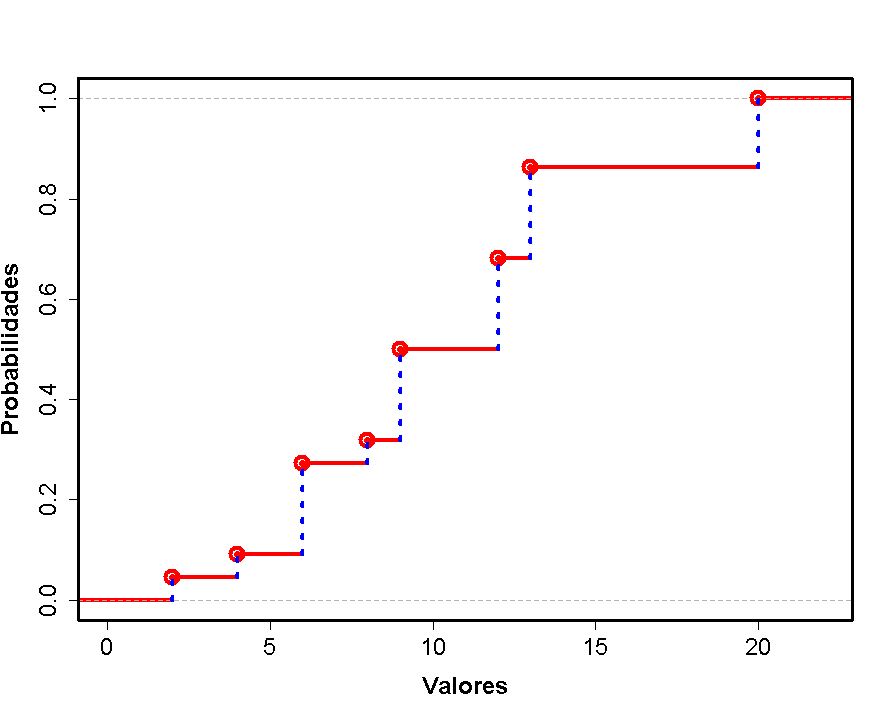
\includegraphics[height=8cm]{../fig/Cap04-FuncionDistribucionVariableAleatoria.png}
	\end{enColor}
	\begin{bn}
    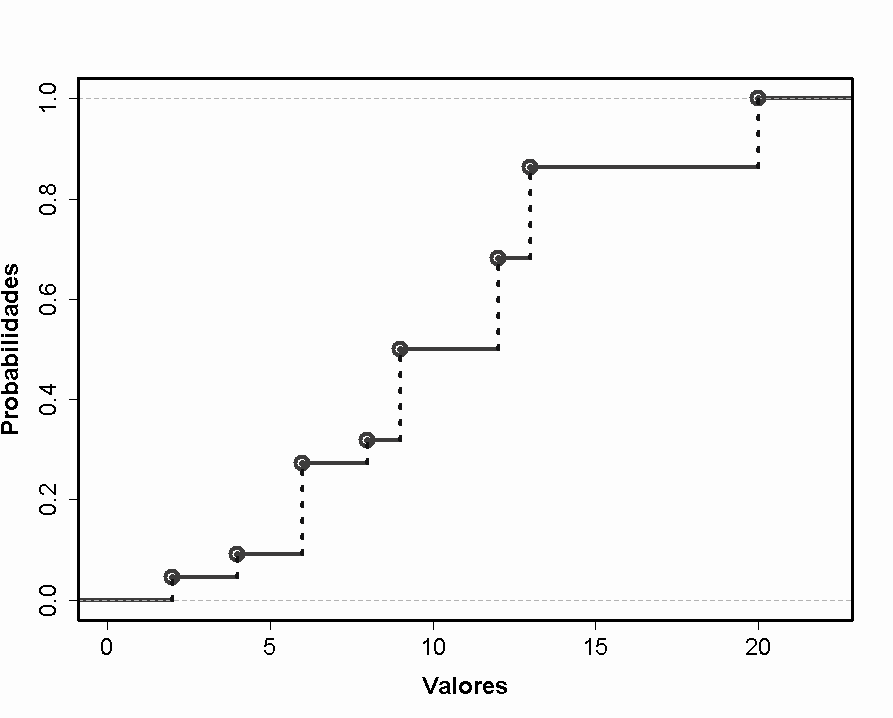
\includegraphics[height=8cm]{../fig/Cap04-FuncionDistribucionVariableAleatoria-bn.png}
	\end{bn}
	\caption{Una ``típica'' función de distribución de una variable aleatoria discreta}
	\label{cap04:fig:GraficaFuncionDistribucionVariableAleatoriaDiscreta}
    \end{figure}

\subsection{Cuantiles de una variable aleatoria discreta.}
\label{cap04:subsec:CuantilesVariableAleatoriaDiscreta}
%\noindent{\bf Opcional: puede omitirse en una primera lectura.}\\
La Figura \ref{cap04:fig:GraficaFuncionDistribucionVariableAleatoriaDiscreta} (pág. \pageref{cap04:fig:GraficaFuncionDistribucionVariableAleatoriaDiscreta}) ayuda a entender que, si fijamos una probabilidad $p_0$ cualquiera, cuanto tratemos de resolver la siguiente ecuación en $x$:
\[F(x)=p_0\]
la mayor parte de las veces no podremos encontrar una solución. No hay solución, salvo que $p_0$ sea $0$, o uno de los valores $p_1$, $p_1+p_2$, \ldots, $1$, que definen la altura de los peldaños. Mencionamos esto aquí como advertencia,  porque cuando estudiemos las variables aleatorias continuas, veremos que allí la situación es distinta y ese tipo de ecuaciones siempre tienen solución. En el caso que ahora nos ocupa, el de las variables aleatorias discretas, con un número finito de valores como la de la Tabla \ref{cap04:tabla:tablaDistribucionProbabilidadGenericaVariableAleatoriaDiscreta}, tenemos que aprender a ser más cautos cuando trabajamos con la función de distribución $F$. De momento nos conformamos con la advertencia, pero profundizaremos más en las consecuencias de este hecho más adelante. Concretamente, en el Capítulo \ref{cap:TeoremaCentralLimite}, al hacer inferencia para la Distribución Binomial, cuando esta discusión se convertirá en un problema más acuciante.
%    \begin{figure}[b!]
%	\centering
%	\begin{enColor}
%    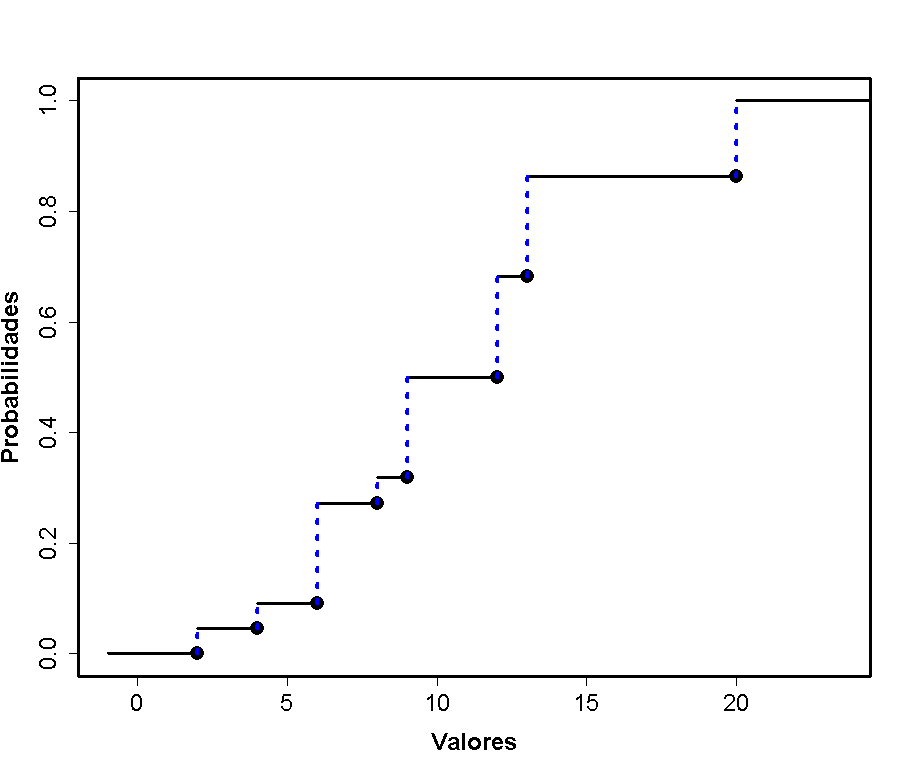
\includegraphics[height=8cm]{../fig/Cap04-PseudoFuncionDistribucionVariableAleatoria.png}
%	\end{enColor}
%	\begin{bn}
%    \includegraphics[height=8cm]{../fig/Cap04-PseudoFuncionDistribucionVariableAleatoria-bn.png}
%	\end{bn}
%	\caption{Usando $<$ en lugar de $\leq$ al acumular la probabilidad de una variable aleatoria discreta}
%	\label{cap04:fig:GraficaPseudoFuncionDistribucionVariableAleatoriaDiscreta}
%    \end{figure}

Puesto que la igualdad $F(x)=p_0$ puede no tener solución, lo que haremos, dada una probabilidad  $p_0$, es considerar la desigualdad
\[F(x)\geq p_0\]
La Figura \ref{cap04:fig:GraficaFuncionDistribucionVariableAleatoriaDiscreta} ayuda a entender que, sea cual sea la probabilidad $p_0$ entre $0$ y $1$, esa desigualdad tiene solución. La dificultad, ahora, es que tiene demasiadas, porque $F$ es constante por intervalos. Es decir, $F$ vale lo mismo para todos los $x$ que quedan debajo de cada uno de los peldaños de la Figura \ref{cap04:fig:GraficaFuncionDistribucionVariableAleatoriaDiscreta}. La solución es utilizar el extremo izquierdo de esos intervalos. Concretamente, la definición es esta:
    \begin{center}
    \fcolorbox{black}{Gris025}{
    \begin{minipage}{12cm}
        \begin{center}
        {\bf Cuantil $p_0$ de una variable aleatoria discreta}
        \index{cuantil de una variable aleatoria discreta}
        \end{center}
        Si $X$ es una variable aleatoria discreta, cuya función de distribución es $F(x)$, entonces, dada una probabilidad $p_0$ cualquiera, el {\sf cuantil} $p_0$ de $X$ es {\bf el menor valor} $x^*$ (técnicamente, el ínfimo de los $x^*$) que cumple:
        \begin{equation}
        \label{cap04:ecu:CuantilVariableAleatoriaDiscreta}
            F(x^*)\geq p_0.
        \end{equation}
    \end{minipage}}
    \end{center}
%Hemos definido la función de distribución usando la desigualdad $\leq$. Si usamos la desigualdad estricta $<$, para  definir otra función:
%\[H(x)=P(X < x )\]
%la gráfica en escalera que se obtiene es similar, como muestra la Figura \ref{cap04:fig:GraficaPseudoFuncionDistribucionVariableAleatoriaDiscreta}, sólo que ahora los puntos sólidos {\em ``han caído''} al segmento inferior, ocupando su extremo derecho. En particular, usando esas dos figuras como ayuda, se comprende que, dada cualquier probabilidad $p_0$, existe un único valor $x^*$ (de entre los valores que toma la variable aleatoria $X$) tal que
%\[H(x^*) < p_0 \leq F(x^*).\]
%Para verlo imagínate un segmento horizontal, situado a altura $p_0$, que recorre de abajo a arriba el intervalo $[0,1]$. En cualquier momento, el segmento está entre uno de los puntos situados en el extremo derecho de un segmento de la Figura \ref{cap04:fig:GraficaPseudoFuncionDistribucionVariableAleatoriaDiscreta}, y el punto situado justo encima, en el extremo izquierdo de uno de los intervalos en la Figura \ref{cap04:fig:GraficaFuncionDistribucionVariableAleatoriaDiscreta}. Esos dos puntos están situados ambos sobre el valor $x^*$ del eje de abscisas.
%
%Este valor $x^*$ es el {\sf cuantil} $p_0$\index{cuantil de una variable aleatoria discreta} de la variable $X$. Otra manera equivalente de definirlo es diciendo que el $x^*$ es el {\em menor valor} para el que se cumple
%\[F(x^*) \geq p_0,\]
%y mientras $p_0$ sea una probabilidad, siempre existe ese valor $x^*$.
Así que, remitiéndonos de nuevo a la Figura \ref{cap04:fig:GraficaFuncionDistribucionVariableAleatoriaDiscreta}, los cuantiles son las coordenadas $x$ de los puntos sólidos que aparecen en los extremos izquierdos de los segmentos horizontales, en esa figura. Por supuesto, coinciden con los valores $x_1$,\ldots,$x_k$ que toma la variable aleatoria $X$. La parte más interesante de la definición de cuantil es la correspondencia que establecemos de probabilidades a valores:
\[ \mbox{Probabilidad } p_0   \dashrightarrow x_i, \mbox{ el valor que es el cuantil de }p_0, \]
Esta correspondencia es, de alguna forma, la correspondencia inversa de la asignación
\[ \mbox{ valor }x \dashrightarrow \mbox{ probabilidad acumulada }F(x)\]
que hace la función de distribución $F$. Y decimos ``de alguna manera'' porque el camino:
\[
    (\mbox{ valor } x)\,\dashrightarrow\, (\mbox{probabilidad }p_0=F(x))\,\dashrightarrow (\mbox{ cuantil de }p_0)
\]
en la mayoría de los casos no nos llevará de vuelta al valor $x$  con el que hemos comenzado, sino al valor más cercano a $x$, por la izquierda, de entre los valores $x_1$,\ldots,$x_k$ que toma la variable $X$. La Figura \ref{cap04:fig:GraficaFuncionDistribucionVariableAleatoriaDiscreta} puede ayudar a entender esto. Y veremos ejemplos más adelante, al tratar sobre la Distribución Binomial en el Capítulo \ref{cap:TeoremaCentralLimite}.



\section{Independencia y vectores aleatorios discretos.}
\label{cap04:sec:IndependenciaVariablesAleatoriasDiscretas}
\noindent{\bf Opcional: esta sección puede omitirse en una primera lectura.}\\

%El contenido de esta sección no es imprescindible para seguir adelante en el curso. Por otra parte, la discusión es necesariamente más técnica, y puede que requiera del lector un esfuerzo adicional que tal vez sea mejor reservar, para el momento en que se haya ganado algo más de confianza con los conceptos de este capítulo. Así que la sección puede omitirse en una primera lectura. No obstante, hemos preferido mantenerla en este capítulo, porque es su sitio natural (o porque no sabríamos donde ponerla, de otra manera...)

Ya sabemos lo que significa que dos sucesos sean independientes. Y ahora vamos a tratar de extender esa misma noción de independencia a las variables aleatorias. La idea intuitiva es la misma. Dos variables aleatorias, $X$ e $Y,$ serán independientes si el conocimiento que tenemos sobre el valor de $X$ no afecta de ninguna manera al que tenemos sobre el valor de $Y$.

Esa idea informal está muy bien, pero ya vimos en su momento que cuando tratábamos de concretarlo, en el caso de los sucesos, necesitábamos la noción de probabilidad condicionada que, a su vez, descansa, en última instancia, sobre la {\em intersección} de los sucesos. La intersección es lo que ambos sucesos tienen en común. Es algo que caracteriza {\em conjuntamente} a la pareja formada por dos sucesos.

Para poder llevar esa misma idea al caso de dos variables aleatorias $X$ e $Y$ vamos a tener que aprender a pensar también en ambas variables {\em conjuntamente}. Esto puede parecer complicado. Pero, de hecho, al igual que sucede con la probabilidad condicionada, a menudo resulta más sencillo trabajar con las propiedades conjuntas de dos variables, que tratar de hacerlo por separado.  {!`}Especialmente cuando son dependientes, claro!

Vamos a pensar entonces en la pareja formada por las variables $X$ e $Y$, y para representar esa pareja usaremos la notación $(X,Y)$. El trabajo que vamos a hacer en este apartado se extiende con relativa facilidad al caso de $k$ variables aleatorias, pensadas conjuntamente, como un objeto que se representa
\[(X_1,\ldots,X_k).\]
Esta clase de objetos se llaman a menudo {\sf vectores aleatorios}\index{vector aleatorio} (en inglés, {\em random vector}\index{random vector}). El número de componentes $k$ es la {\sf dimensión} del vector aleatorio; de manera que, por ejemplo, $(X,Y)$ será un vector aleatorio bidimensional. Un vector aleatorio $(X,Y)$ que sólo toma una cantidad finita de valores es un {\sf vector aleatorio discreto}\index{vector aleatorio discreto}.

Ya hemos visto que una variable aleatoria $X$ queda caracterizada por su tabla o función de densidad (ver pág. \pageref{cap04:ecu:funcionDensidadVariableAleatoriaDiscreta}). Esa tabla nos dice, para cada uno de los valores $x_i$ que puede tomar la variable, cuál es la probabilidad $p_i$ de que $X$ tome ese valor. Cuando se trata de una pareja $(X,Y)$ existe un objeto análogo, que es la función de densidad conjunta de $X$ e $Y$.
    \begin{center}
    \fcolorbox{black}{Gris025}{
    \begin{minipage}{12cm}
        \begin{center}
        {\bf Función de densidad conjunta de un vector aleatorio discreto.}
        \end{center}
        \index{función de densidad conjunta de un vector aleatorio discreto}
        Si $(X, Y)$ es un vector aleatorio discreto, que sólo toma una cantidad finita de valores,        su {\sf función de densidad conjunta} es la función definida mediante:
        \begin{equation}
        \label{cap04:ecu:FuncionDensidadConjuntaVectorAleatorio}
        f(x,y)=P\bigg((X, Y) =(x, y)\bigg) = P(X=x, Y=y).
        \end{equation}
        (Hemos usado dos notaciones para intentar aclarar la definición. La segunda es la más habitual.) Es decir, la función $f$ nos dice cuál es la probabilidad de que el vector $(X,Y)$ tome el valor $(x,y)$. Al ser $(X,Y)$ discreto, sólo existe una cantidad finita de parejas $(x,y)$ para las que esta probabilidad es distinta de $0$.
    %\end{definicion}
    \end{minipage}}
    \end{center}
\quad\\
Veamos un primer ejemplo sencillo, con variables que ya hemos encontrado antes.
\begin{ejemplo}
\label{cap04:ejem:VectoAleatorioDiscretoDado}
En el Ejemplo \ref{cap04:ejem:varianzaSumaVariablesAleatoriasDiscretas} hemos dejado pendiente la cuestión de si, en el caso del lanzamiento de dos dados, las variables $X$ (suma) e $Y$ (diferencia, en valor absoluto) son o no independientes. Todavía tenemos que definir lo que significa la independencia en este contexto. En el Ejemplo \ref{cap04:ejem:IndependenciaVariablesAleatoriasDiscretas} volveremos sobre esa cuestión. Ahora, para preparar el terreno, vamos a construir la tabla o función de densidad conjunta de ambas variables. Para ayudarnos a ver cuál es esa tabla vamos a pensar en el espacio muestral formado por los $36$ posibles resultados al lanzar dos dados. La parte (a) de la Tabla \ref{cap04:tabla:VectoAleatorioDiscretoDado} (pág. \pageref{cap04:tabla:VectoAleatorioDiscretoDado}) muestra en cada fila uno de esos $36$ resultados, y para cada resultado se muestran, en las dos últimas columnas de la tabla, los valores de $X$ e $Y$.

Esas dos últimas columnas nos proporcionan la información que necesitamos sobre la densidad conjunta del vector $(X,Y)$. Tenemos 36 pares de valores $(X, Y)$, pero que no son todos distintos los unos de los otros. Después de ver cuántos pares distintos hay, y cuántas veces aparece cada uno de ellos, la parte (b) de la la Tabla \ref{cap04:tabla:VectoAleatorioDiscretoDado} usa esa información para mostrar la probabilidad de aparición de cada uno de esos pares. Esa tabla describe, por tanto, la función de densidad conjunta del vector $(X, Y)$. Y nos dice, por ejemplo, que
\[f(5,3) = P(X=5, Y=3) = \dfrac{2}{36}.\]
Si quieres, puedes buscar en la parte (a) de la tabla cuales son los dos puntos del espacio muestral que corresponden a este resultado. Fíjate, en la parte (b) de la Tabla \ref{cap04:tabla:VectoAleatorioDiscretoDado} en que, aunque $X$ puede tomar el valor $6$, e $Y$ puede tomar el valor $1$, para la densidad conjunta es $f(6,1)=0$.

\begin{table}[p]
\begin{center}
\begin{tabular}{cc}
(a) & (b)\\[5mm]
{\scriptsize
\begin{tabular}{|c|c|c|c|}
  \hline
dado1 & dado2 & X & Y \\
  \hline
  1 &   1 &   2 &   0 \\ \hline
    2 &   1 &   3 &   1 \\ \hline
    3 &   1 &   4 &   2 \\ \hline
    4 &   1 &   5 &   3 \\ \hline
    5 &   1 &   6 &   4 \\ \hline
    6 &   1 &   7 &   5 \\ \hline
    1 &   2 &   3 &   1 \\ \hline
    2 &   2 &   4 &   0 \\ \hline
    3 &   2 &   5 &   1 \\ \hline
    4 &   2 &   6 &   2 \\ \hline
    5 &   2 &   7 &   3 \\ \hline
    6 &   2 &   8 &   4 \\ \hline
    1 &   3 &   4 &   2 \\ \hline
    2 &   3 &   5 &   1 \\ \hline
    3 &   3 &   6 &   0 \\ \hline
    4 &   3 &   7 &   1 \\ \hline
    5 &   3 &   8 &   2 \\ \hline
    6 &   3 &   9 &   3 \\ \hline
    1 &   4 &   5 &   3 \\ \hline
    2 &   4 &   6 &   2 \\ \hline
    3 &   4 &   7 &   1 \\ \hline
    4 &   4 &   8 &   0 \\ \hline
    5 &   4 &   9 &   1 \\ \hline
    6 &   4 &  10 &   2 \\ \hline
    1 &   5 &   6 &   4 \\ \hline
    2 &   5 &   7 &   3 \\ \hline
    3 &   5 &   8 &   2 \\ \hline
    4 &   5 &   9 &   1 \\ \hline
    5 &   5 &  10 &   0 \\ \hline
    6 &   5 &  11 &   1 \\ \hline
    1 &   6 &   7 &   5 \\ \hline
    2 &   6 &   8 &   4 \\ \hline
    3 &   6 &   9 &   3 \\ \hline
    4 &   6 &  10 &   2 \\ \hline
    5 &   6 &  11 &   1 \\ \hline
    6 &   6 &  12 &   0 \\
   \hline
\end{tabular}
}
&
\begin{tabular}[b]{c|r|r|r|r|r|r|r|}
  \multicolumn{1}{c}{}&\multicolumn{1}{c}{}&\multicolumn{6}{c}{Valor de $Y$}\\
  \cline{3-8}
  \multicolumn{1}{c}{}
  && 0 & 1 & 2 & 3 & 4 & 5 \\  \cline{2-8}
  \multirow{10}{*}{
  \rotatebox{90}{Valor de $X$}
  }
    &   2 & 1/36 & 0 & 0 & 0 & 0 & 0 \\ \cline{2-8}
    &   3 & 0 & 1/18 & 0 & 0 & 0 & 0 \\ \cline{2-8}
    &   4 & 1/36 & 0 & 1/18 & 0 & 0 & 0 \\ \cline{2-8}
    &   5 & 0 & 1/18 & 0 & 1/18 & 0 & 0 \\ \cline{2-8}
    &   6 & 1/36 & 0 & 1/18 & 0 & 1/18 & 0 \\ \cline{2-8}
    &   7 & 0 & 1/18 & 0 & 1/18 & 0 & 1/18 \\ \cline{2-8}
    &   8 & 1/36 & 0 & 1/18 & 0 & 1/18 & 0 \\ \cline{2-8}
    &   9 & 0 & 1/18 & 0 & 1/18 & 0 & 0 \\ \cline{2-8}
    &   10 & 1/36 & 0 & 1/18 & 0 & 0 & 0 \\ \cline{2-8}
    &   11 & 0 & 1/18 & 0 & 0 & 0 & 0 \\ \cline{2-8}
    &   12 & 1/36 & 0 & 0 & 0 & 0 & 0 \\
   \cline{2-8}
\end{tabular}
\end{tabular}

%(a)\\[3mm]
%{\scriptsize
%\begin{tabular}{|c|c|c|c|}
%  \hline
%dado1 & dado2 & X & Y \\
%  \hline
%  1 &   1 &   2 &   0 \\ \hline
%    2 &   1 &   3 &   1 \\ \hline
%    3 &   1 &   4 &   2 \\ \hline
%    4 &   1 &   5 &   3 \\ \hline
%    5 &   1 &   6 &   4 \\ \hline
%    6 &   1 &   7 &   5 \\ \hline
%    1 &   2 &   3 &   1 \\ \hline
%    2 &   2 &   4 &   0 \\ \hline
%    3 &   2 &   5 &   1 \\ \hline
%    4 &   2 &   6 &   2 \\ \hline
%    5 &   2 &   7 &   3 \\ \hline
%    6 &   2 &   8 &   4 \\ \hline
%    1 &   3 &   4 &   2 \\ \hline
%    2 &   3 &   5 &   1 \\ \hline
%    3 &   3 &   6 &   0 \\ \hline
%    4 &   3 &   7 &   1 \\ \hline
%    5 &   3 &   8 &   2 \\ \hline
%    6 &   3 &   9 &   3 \\ \hline
%    1 &   4 &   5 &   3 \\ \hline
%    2 &   4 &   6 &   2 \\ \hline
%    3 &   4 &   7 &   1 \\ \hline
%    4 &   4 &   8 &   0 \\ \hline
%    5 &   4 &   9 &   1 \\ \hline
%    6 &   4 &  10 &   2 \\ \hline
%    1 &   5 &   6 &   4 \\ \hline
%    2 &   5 &   7 &   3 \\ \hline
%    3 &   5 &   8 &   2 \\ \hline
%    4 &   5 &   9 &   1 \\ \hline
%    5 &   5 &  10 &   0 \\ \hline
%    6 &   5 &  11 &   1 \\ \hline
%    1 &   6 &   7 &   5 \\ \hline
%    2 &   6 &   8 &   4 \\ \hline
%    3 &   6 &   9 &   3 \\ \hline
%    4 &   6 &  10 &   2 \\ \hline
%    5 &   6 &  11 &   1 \\ \hline
%    6 &   6 &  12 &   0 \\
%   \hline
%\end{tabular}
%}\\[3mm]
%(b)\\[3mm]
%\begin{tabular}{rllllll}
%  \hline
% & 0 & 1 & 2 & 3 & 4 & 5 \\
%  \hline
%2 & 1/36 & 0 & 0 & 0 & 0 & 0 \\
%  3 & 0 & 1/18 & 0 & 0 & 0 & 0 \\
%  4 & 1/36 & 0 & 1/18 & 0 & 0 & 0 \\
%  5 & 0 & 1/18 & 0 & 1/18 & 0 & 0 \\
%  6 & 1/36 & 0 & 1/18 & 0 & 1/18 & 0 \\
%  7 & 0 & 1/18 & 0 & 1/18 & 0 & 1/18 \\
%  8 & 1/36 & 0 & 1/18 & 0 & 1/18 & 0 \\
%  9 & 0 & 1/18 & 0 & 1/18 & 0 & 0 \\
%  10 & 1/36 & 0 & 1/18 & 0 & 0 & 0 \\
%  11 & 0 & 1/18 & 0 & 0 & 0 & 0 \\
%  12 & 1/36 & 0 & 0 & 0 & 0 & 0 \\
%   \hline
%\end{tabular}
%{\small
%\begin{tabular}{l|c|c|c|c|c|c|c|c|c|c|c|c|}
%  \multicolumn{2}{c}{}
%  &\multicolumn{11}{c}{Valor de $X$}\\
%  \cline{3-13}
%
%  \multicolumn{2}{c|}{}
% & 2 & 3 & 4 & 5 & 6 & 7 & 8 & 9 & 10 & 11 & 12 \\
%  \cline{2-13}
%\multirow{6}{*}{
%\begin{minipage}{0.8cm}
%{\small
%Valor\\ de $Y$
%}
%\end{minipage}
%}
%& 0 &   $1/36$ &   0 &   $1/36$ &   0 &   $1/36$ &   0 &   $1/36$ &   0 &   $1/36$ &   0 &   $1/36$ \\ \cline{2-13}
%&  1 &   0 &   $2/36$ &   0 &   $2/36$ &   0 &   $2/36$ &   0 &   $2/36$ &   0 &   $2/36$ &   0 \\ \cline{2-13}
%&  2 &   0 &   0 &   $2/36$ &   0 &   $2/36$ &   0 &   $2/36$ &   0 &   $2/36$ &   0 &   0 \\ \cline{2-13}
%&  3 &   0 &   0 &   0 &   $2/36$ &   0 &   $2/36$ &   0 &   $2/36$ &   0 &   0 &   0 \\ \cline{2-13}
%&  4 &   0 &   0 &   0 &   0 &   $2/36$ &   0 &   $2/36$ &   0 &   0 &   0 &   0 \\ \cline{2-13}
%&  5 &   0 &   0 &   0 &   0 &   0 &   $2/36$ &   0 &   0 &   0 &   0 &   0 \\
%   \cline{2-13}
%\end{tabular}
%}
\end{center}
\caption{Ejemplo \ref{cap04:ejem:VectoAleatorioDiscretoDado}. (a) Los valores de $X$ e $Y$ en cada punto del espacio muestral. (b) La tabla de densidad conjunta de $X$ e $Y$.}
\label{cap04:tabla:VectoAleatorioDiscretoDado}
\end{table}
Algunas preguntas en las que puedes ir pensando:
\begin{enumerate}
  \item ¿Cuánto vale la suma de todos los elementos de la Tabla \ref{cap04:tabla:VectoAleatorioDiscretoDado}(b)?
  \item Usando la la Tabla \ref{cap04:tabla:VectoAleatorioDiscretoDado}(b) (y sólo esa tabla) ¿cómo calcularías la probabilidad de que $Y$ tome el valor $2$ (sea cual sea el valor de $X$)?
  \item ¿Crees (intuitivamente) que $X$ e $Y$, en este ejemplo, son independientes?
\end{enumerate}
Volveremos sobre estas preguntas en breve.
\qed
\end{ejemplo}

\subsubsection{Aclaraciones sobre la representación como tabla o como función de la densidad conjunta.}

En el Ejemplo \ref{cap04:ejem:VectoAleatorioDiscretoDado} hemos visto una forma bastante habitual de presentar la tabla de densidad conjunta de un vector aleatorio $(X,Y)$. Si $X$ toma los valores $x_1,\ldots,x_k$, mientras que $Y$ toma los valores $y_1,\ldots,y_m$, entonces podemos hacer una tabla de doble entrada, como la Tabla \ref{cap04:tabla:DensidadConjuntaVectorAleatorioDiscreto}
\begin{table}[h!]
\[
\hspace{-1cm}\mbox{Valor de $X$}\quad\begin{array}{|c|c|c|c|c|}
\multicolumn{1}{c}{} &\multicolumn{4}{c}{\mbox{Valor de $Y$}}{}\\
\cline{2-5}
\multicolumn{1}{c|}{} &y_1    & y_2   & \cdots    & y_m\\
    \hline
x_1 &p_{11} & p_{12}& \cdots    & p_{1m}\\
    \hline
x_2 &p_{21} & p_{22}& \cdots    & p_{2m}\\
\hline
\vdots&     &       & \ddots    &       \\
    \hline
x_k &p_{k1} & p_{k2}& \cdots    & p_{km}\\
    \hline
\end{array}
\]
\caption{Tabla de densidad conjunta de probabilidad para un vector aleatorio discreto $(X,Y)$.}
\label{cap04:tabla:DensidadConjuntaVectorAleatorioDiscreto}
\end{table}
en la que $f(x_i,y_j)=p_{ij}$. Naturalmente, como muestra el ejemplo, puede haber pares $(x_i,y_j)$ tales que $f(x_i,y_j)=0$, aunque las probabilidades $P(X=x_i)$ y $P(y=y_j)$ sean ambas no nulas.

Una aclaración más, para evitar posibles confusiones: cuando decimos que $X$ toma los valores $x_1,\ldots,x_k$, queremos decir que si $x_0$ {\em no} es uno de los valores $x_1,\ldots,x_k$, entonces, sea cual sea el valor de $y_0$, se cumple {\em automáticamente:}
\[
f(x_0,y_0)=0.
\]
Y lo mismo sucede si $y_0$ no es uno de los valores $y_1,\ldots,y_m$. Entonces, sea cual sea $x_0$, la densidad conjunta $f(x_0,y_0)$ es automáticamente nula.

\noindent Por si estás cansado de ejemplos con dados (paciencia, aún nos quedan unos cuantos en el curso...), hemos incluido otro ejemplo, que puedes encontrar más interesante.
\begin{ejemplo}
\label{cap04:ejem:vectorAleatorioDias2014}
Imagínate que el departamento de control de calidad de una gran empresa quiere realizar un estudio sobre su servicio de atención al cliente, para saber si los recursos asignados a ese servicio son suficientes. Si la empresa es grande, puede que el servicio haya atendido decenas de miles de peticiones a lo largo de un año. Y puede resultar poco práctico tratar de analizarlas todas. Para hacerse una idea rápida, se podrían seleccionar  al azar $30$ días del año, y analizar el funcionamiento del servicio en esos días. Ya volveremos sobre estas ideas más adelante, pero el hecho de seleccionar los días al azar es esencial, para garantizar que el conjunto de días seleccionados  es {\em representativo} y reducir la posible influencia de factores desconocidos. Por ejemplo si todos los días seleccionados fueran viernes o si se seleccionan varios días en los que hubo grandes averías del servicio telefónico, la muestra no sería representativa. La selección al azar hace muy improbable elegir una muestra así.

Para llevar adelante este plan, por tanto, tenemos que seleccionar un día del año al azar. Y después, cuando analicemos los resultados, querremos saber si ese día es laborable, si es viernes o jueves, etc.  Así que vamos a pensar en un experimento en el que elegimos al azar un día del año 2014. Este es el mecanismo básico. Luego bastaría con repetirlo para obtener los 30 días necesarios. Volveremos sobre esto en el Capítulo \ref{cap:IntervalosConfianza}, cuando hablemos de muestreo.

Vamos a considerar el vector aleatorio $(X,Y)$, donde el valor de $X$ indica el día de la semana (desde $1$ para lunes, a $7$ para domingo) , y el valor de $Y$ indica el día del mes. La Tabla \ref{cap04:tabla:vectorAleatorioDias2014} (pág. \pageref{cap04:tabla:vectorAleatorioDias2014}) es una tabla de {\em frecuencia} conjunta de $X$ e $Y$.  No hemos presentado directamente la tabla de densidad conjunta porque creemos que en este caso es más fácil visualizar los datos en forma de frecuencias, y porque el cálculo  de las probabilidades a partir de ahí es inmediato: para conseguir la tabla de densidad del vector aleatorio $(X,Y)$ basta con dividir cada elemento de la Tabla \ref{cap04:tabla:vectorAleatorioDias2014} por $365$.

Para entender más a fondo el ejemplo, veamos cuanto vale
\[f(4, 20) = P(X=4, Y=20).\]
Vamos a la Tabla \ref{cap04:tabla:vectorAleatorioDias2014} y comprobamos que la frecuencia del valor $(X,Y)=(4,20)$ es $3$. Por lo tanto:
\[f(4, 20) = P(X=4, Y=20)=\dfrac{3}{365}.\]
Esto significa que si elegimos un día al azar  del año $2014$, la probabilidad de que sea $X=4$ (el día es jueves) e $Y=20$ (el día elegido es el día $20$ del mes) es de $\frac{3}{365}\approx 0.008219$.

\begin{table}[p]
\centering
$Y=$ día del mes
\begin{tabular}{|r|r|r|r|r|r|r|r|}

  \multicolumn{1}{c}{}&\multicolumn{7}{ c }{$X=$ día de la semana.} \\
  \cline{2-8}
 \multicolumn{1}{c|}{}& 1 & 2 & 3 & 4 & 5 & 6 & 7 \\
  \hline
1 &   2 &   2 &   2 &   1 &   1 &   3 &   1 \\
  2 &   1 &   2 &   2 &   2 &   1 &   1 &   3 \\
  3 &   3 &   1 &   2 &   2 &   2 &   1 &   1 \\
  4 &   1 &   3 &   1 &   2 &   2 &   2 &   1 \\
  5 &   1 &   1 &   3 &   1 &   2 &   2 &   2 \\
  6 &   2 &   1 &   1 &   3 &   1 &   2 &   2 \\
  7 &   2 &   2 &   1 &   1 &   3 &   1 &   2 \\
  8 &   2 &   2 &   2 &   1 &   1 &   3 &   1 \\
  9 &   1 &   2 &   2 &   2 &   1 &   1 &   3 \\
  10 &   3 &   1 &   2 &   2 &   2 &   1 &   1 \\
  11 &   1 &   3 &   1 &   2 &   2 &   2 &   1 \\
  12 &   1 &   1 &   3 &   1 &   2 &   2 &   2 \\
  13 &   2 &   1 &   1 &   3 &   1 &   2 &   2 \\
  14 &   2 &   2 &   1 &   1 &   3 &   1 &   2 \\
  15 &   2 &   2 &   2 &   1 &   1 &   3 &   1 \\
  16 &   1 &   2 &   2 &   2 &   1 &   1 &   3 \\
  17 &   3 &   1 &   2 &   2 &   2 &   1 &   1 \\
  18 &   1 &   3 &   1 &   2 &   2 &   2 &   1 \\
  19 &   1 &   1 &   3 &   1 &   2 &   2 &   2 \\
  20 &   2 &   1 &   1 &   3 &   1 &   2 &   2 \\
  21 &   2 &   2 &   1 &   1 &   3 &   1 &   2 \\
  22 &   2 &   2 &   2 &   1 &   1 &   3 &   1 \\
  23 &   1 &   2 &   2 &   2 &   1 &   1 &   3 \\
  24 &   3 &   1 &   2 &   2 &   2 &   1 &   1 \\
  25 &   1 &   3 &   1 &   2 &   2 &   2 &   1 \\
  26 &   1 &   1 &   3 &   1 &   2 &   2 &   2 \\
  27 &   2 &   1 &   1 &   3 &   1 &   2 &   2 \\
  28 &   2 &   2 &   1 &   1 &   3 &   1 &   2 \\
  29 &   2 &   2 &   2 &   1 &   1 &   2 &   1 \\
  30 &   1 &   2 &   2 &   2 &   1 &   1 &   2 \\
  31 &   1 &   0 &   1 &   1 &   2 &   1 &   1 \\
   \hline
\end{tabular}
\caption{Tabla de frecuencia conjunta de $X$ (día de la semana) e $Y$ día del mes, para el año 2014, en el Ejemplo \ref{cap04:ejem:vectorAleatorioDias2014}.}
\label{cap04:tabla:vectorAleatorioDias2014}
\end{table}
\qed
\end{ejemplo}


\subsection{Densidades marginales.}
\label{cap04:subsec:DendidadesMarginales}

Recuerda que dos sucesos $A$ y $B$ son independientes si se cumple:
\[P(A\cap B)= P(A)\cdot P(B).\]
Ahora queremos trasladar esta definición al caso de un vector aleatorio discreto. La densidad conjunta, que ya hemos definido, va a jugar el papel que  la intersección jugaba en el caso de los sucesos. Pero entonces necesitamos algo que juegue el papel de las probabilidades {\em por separado} de cada una de las componentes $X$ e $Y$ del vector aleatorio. Ese papel lo juegan las densidades marginales.
    \begin{center}
    \fcolorbox{black}{Gris025}{
    \begin{minipage}{12cm}
        \begin{center}
        {\bf Densidades marginales de un vector aleatorio discreto.}
        \end{center}
        Sea $(X, Y)$ es un vector aleatorio discreto, con función de densidad $f$. Supongamos que
        $X$ toma los valores $x_1,\ldots,x_k$ e $Y$ toma los valores $y_1,\ldots,y_m$, en el sentido que hemos precisado antes. Entonces la {\sf función de densidad marginal}\index{función de densidad marginal (caso discreto)}\index{marginal, función de densidad (caso discreto)}\index{densidad marginal, función de (caso discreto)} (en inglés, {\em marginal density}\index{marginal density}) de $X$ es la función definida mediante:
        \begin{equation}
        \label{cap04:ecu:FuncionDensidadMarginalXVectorAleatorio}
        f_X(x)=f(x,y_1)+ f(x,y_2)+\cdots+f(x,y_m)=\underbrace{
        \sum_{j=1}^m f(x, y_j).}_{\mbox{\tiny todos los valores de $y$}}
        \end{equation}
        De la misma forma, la función de densidad marginal de $Y$ es
        \begin{equation}
        \label{cap04:ecu:FuncionDensidadMarginalYVectorAleatorio}
        f_Y(y)=f(x_1,y)+ f(x_2,y)+\cdots+f(x_k,y)=\underbrace{
        \sum_{i=1}^k f(x_i, y).}_{\mbox{\tiny todos los valores de $x$}}
        \end{equation}
    \end{minipage}}
    \end{center}
Como hemos indicado, la densidad marginal de $X$,  para un valor $x$ dado, se obtiene manteniendo fijo ese valor de $x$ y sumando sobre todos los posibles valores de $Y$. La densidad marginal de $Y$ se define igual, intercambiando los papeles de $X$ e $Y$. Veamos un ejemplo.

\begin{ejemplo}
\label{cap04:ejem:densidadesMarginales}
{\bf (Continuación del Ejemplo \ref{cap04:ejem:VectoAleatorioDiscretoDado}, pág. \pageref{cap04:ejem:VectoAleatorioDiscretoDado}).} En la Tabla \ref{cap04:tabla:MarginalesVectoAleatorioDiscretoDado} se muestra el resultado que se obtiene si, partiendo de la Tabla \ref{cap04:tabla:VectoAleatorioDiscretoDado}(b), se suman los valores de cada fila y cada columna, y se colocan en los márgenes de la tabla. Como puede verse, el resultado es que la última columna y la última fila muestran, respectivamente, las densidades marginales de $X$ e $Y$.
\begin{table}[ht]
\begin{center}
{
\rotatebox{90}{Valor de $X$\phantom{12345}}
}
\quad
\begin{tabular}{|r|r|r|r|r|r|r|r|}
  \multicolumn{1}{c}{}&\multicolumn{7}{c}{Valor de $Y$}\\
  \cline{2-8}
  \multicolumn{1}{c|}{}& 0 & 1 & 2 & 3 & 4 & 5 & Suma \\
  \hline
  2 & 1/36 & 0 & 0 & 0 & 0 & 0 & 1/36 \\ \hline
  3 & 0 & 1/18 & 0 & 0 & 0 & 0 & 1/18 \\ \hline
  4 & 1/36 & 0 & 1/18 & 0 & 0 & 0 & 1/12 \\ \hline
  5 & 0 & 1/18 & 0 & 1/18 & 0 & 0 & 1/9 \\ \hline
  6 & 1/36 & 0 & 1/18 & 0 & 1/18 & 0 & 5/36 \\ \hline
  7 & 0 & 1/18 & 0 & 1/18 & 0 & 1/18 & 1/6 \\ \hline
  8 & 1/36 & 0 & 1/18 & 0 & 1/18 & 0 & 5/36 \\ \hline
  9 & 0 & 1/18 & 0 & 1/18 & 0 & 0 & 1/9 \\ \hline
  10 & 1/36 & 0 & 1/18 & 0 & 0 & 0 & 1/12 \\ \hline
  11 & 0 & 1/18 & 0 & 0 & 0 & 0 & 1/18 \\ \hline
  12 & 1/36 & 0 & 0 & 0 & 0 & 0 & 1/36 \\ \hline
  Suma & 1/6 & 5/18 & 2/9 & 1/6 & 1/9 & 1/18 & 1 \\
   \hline
\end{tabular}
\end{center}
\caption{Densidades marginales de $X$ e $Y$ para el vector aleatorio del Ejemplo \ref{cap04:ejem:VectoAleatorioDiscretoDado}.}
\label{cap04:tabla:MarginalesVectoAleatorioDiscretoDado}
\end{table}
\qed
\end{ejemplo}
La forma en la que se obtienen las densidades marginales a partir de la tabla de densidad conjunta explica el origen del nombre {\em marginales}; son los valores que aparecen en los márgenes de la tabla. La interpretación de las densidades marginales en términos de probabilidades es extremadamente simple, pero conviene detenerse a pensar un momento en ella:
\begin{equation}
\label{cap04:ecu:DensidadMarginalXInterpretacionProababilistica}
f_X(x)=P(X=x).
\end{equation}
La probabilidad del miembro derecho debe entenderse, en este contexto como ``la probabilidad de que se cumpla $X=x$, sin importar cuál sea el valor de $Y$''.

En el caso $n$-dimensional, la densidad marginal de $X_i$ en el vector aleatorio $(X_1,\ldots, X_n)$ se obtiene sumando sobre todas las componentes, salvo precisamente la $i$.

Para cerrar este apartado, señalaremos que las densidades marginales contienen la respuesta a las dos primeras preguntas que dejamos pendiente en el Ejemplo \ref{cap04:ejem:VectoAleatorioDiscretoDado} (pág. \pageref{cap04:ejem:VectoAleatorioDiscretoDado}).

\subsubsection{Suma total de una tabla de densidad conjunta.}

En cuanto a la primera pregunta pendiente del Ejemplo \ref{cap04:ejem:VectoAleatorioDiscretoDado}, el resultado de la celda inferior derecha de la Tabla \ref{cap04:tabla:MarginalesVectoAleatorioDiscretoDado} anticipa la respuesta. Puesto que, en última instancia, estamos estudiando la probabilidad de todos los valores posibles, las tablas de densidad conjunta de un vector aleatorio tienen siempre la propiedad de que la suma de todos los elementos de la tabla vale $1$. Puedes comprobar esto sumando los valores de las tablas de los Ejemplos \ref{cap04:ejem:VectoAleatorioDiscretoDado} y \ref{cap04:ejem:vectorAleatorioDias2014}. Para facilitar el trabajo, en el Tutorial04 veremos como usar el ordenador para hacer esto.

\subsubsection{Función de distribución de un vector aleatorio.}

La {\sf función de distribución de un vector aleatorio} se define de una manera similar a la de una variable aleatoria. Si $(X,Y)$ es el vector aleatorio, y $(x_0,y_0)$ es un par de valores cualesquiera, su función de distribución $F$ se define mediante:
\begin{equation}
\label{cap04:ecu:FuncionDistribucionVectorAleatorio}
F(x_0, y_0) = P(X\leq x_0, Y\leq y_0)=P\bigg((X\leq x_0)\cap(Y\leq y_0)\bigg).
\end{equation}
Hemos incluido las dos notaciones porque, aunque la de la intersección es la más precisa de las dos, la notación con la coma es la más usada, y en general no provoca errores. Las {\sf funciones de distribución marginales}\index{funciones de distribución marginales (caso discreto)} $F_X(x)$ y $F_Y(y)$ se definen como las densidades marginales, reemplazando en las Ecuaciones \ref{cap04:ecu:FuncionDensidadMarginalXVectorAleatorio} y \ref{cap04:ecu:FuncionDensidadMarginalYVectorAleatorio} (pág. \pageref{cap04:ecu:FuncionDensidadMarginalYVectorAleatorio}) la $f$ (densidad) por $F$ (distribución).


\subsection{Independencia.}
\label{cap04:subsec:IndependenciaVectorAleatorioDiscreto}

Las densidades marginales juegan el papel de {\em ``cada variable por separado''}, así que ya tenemos todos los ingredientes necesarios para la definición de independencia de un vector aleatorio.

    \begin{center}
    \fcolorbox{black}{Gris025}{
    \begin{minipage}{12cm}
    %\begin{definicion}
        \begin{center}
        {\bf Independencia de variables aleatorias discretas.}
        \end{center}
        \index{independencia de dos variables aleatorias discretas}
        Sea $(X,Y)$ un vector aleatorio discreto, con función de densidad conjunta $f(x,y)$, y con densidades marginales $f_X(x)$ y $f_Y(y)$. Las variables aleatorias discretas $X$ e $Y$ son {\sf independientes} si, sea cual sea el par de valores $(x,y)$ que se considere, se cumple:
        \begin{equation}
        \label{cap04:ecu:indepedenciaVariablesAleatoriasDiscretas}
        f(x,y)=f_X(x)\cdot f_Y(y).
        \end{equation}
        En términos de las funciones de distribución, esto es equivalente a que sea:
        \begin{equation}
        \label{cap04:ecu:indepedenciaVariablesAleatoriasDiscretasFDistribucion}
        F(x,y)=F_X(x)\cdot F_Y(y).
        \end{equation}
    %\end{definicion}
    \end{minipage}}
    \end{center}
En el caso de un vector aleatorio $n$ dimensional, como $(X_1,X_2,\ldots,X_n)$, la independencia significa que la densidad conjunta es el producto de las $n$ densidades marginales:
\begin{equation}
\label{cap04:ecu:indepedenciaVariablesAleatoriasDiscretasCasoNdimensional}
f(x_1,x_2,\ldots,x_n) = f_{X_1}(x_1)\cdot f_{X_2}(x_2)\cdot\,\cdots\,\cdot f_{X_n}(x_n)
\end{equation}
En este caso, a diferencia de lo que sucedía con la independencia de sucesos, para probar la independencia basta con esto y no es necesario considerar productos dos a dos, tres a tres, etc. Si quieres más detalles tendrás que consultar un libro de Estadística Matemática, como por ejemplo \cite{horra2003estadistica} o \cite{Shao_2003_book}.


¿Cómo se puede comprobar la independencia, a partir de la tabla de densidad conjunta? En dos pasos:
\begin{enumerate}
  \item Calculando las densidades marginales $f_X$ y $f_Y$.
  \item Para cada valor $p_{ij}=f(x_i,y_j)$ de la tabla tenemos que comprobar si se cumple la Ecuación \ref{cap04:ecu:indepedenciaVariablesAleatoriasDiscretas}. Es decir, si ese valor es igual al producto de los valores marginales correspondientes a su fila y a su columna.
\end{enumerate}
Es más fácil decirlo que hacerlo. Si la variable $X$ toma $k$ valores, y la variable $Y$ toma $m$ valores, hay que hacer $k\cdot m$ comprobaciones. Y por supuesto, basta con que uno de esos productos no cumpla la Ecuación \ref{cap04:ecu:indepedenciaVariablesAleatoriasDiscretas} para poder asegurar que $X$ e $Y$ no son independientes.


\begin{ejemplo}
\label{cap04:ejem:IndependenciaVariablesAleatoriasDiscretas}
En el ejemplo \ref{cap04:ejem:varianzaSumaVariablesAleatoriasDiscretas} hemos dejado pendiente la cuestión de si, en el caso del lanzamiento de dos dados, las variables $X$ (suma) e $Y$ (diferencia, en valor absoluto) son o no independientes. En la Tabla \ref{cap04:tabla:MarginalesVectoAleatorioDiscretoDado} (pág. \pageref{cap04:tabla:MarginalesVectoAleatorioDiscretoDado}) tenemos tanto la densidad conjunta como las densidades marginales de este ejemplo. Y en este caso, basta con fijarse con el primer valor de la tabla, el situado en la esquina superior izquierda. Ahí vemos que la densidad conjunta vale:
\[f(X=2, Y=0)=\dfrac{1}{36},\]
mientras que las densidades marginales son:
\[
f_X(2)=\dfrac{1}{36},\qquad f_Y(0)=\dfrac{1}{6}.
\]
Así que está claro que en ese caso no se cumple la Ecuación \ref{cap04:ecu:indepedenciaVariablesAleatoriasDiscretas}. Por lo tanto, sin necesidad de más comprobaciones, ya podemos asegurar que $X$ e $Y$ no son independientes. La información sobre el resultado de una de las variables condiciona a la otra variable. Fíjate en que, por ejemplo, si sabes que la diferencia $Y$ es cero, la suma $X$ ya no puede ser impar.
\qed
\end{ejemplo}
Naturalmente, en muchos casos las cosas serán más complicadas. Por ejemplo, en un caso como el del Ejemplo \ref{cap04:ejem:vectorAleatorioDias2014}, si las variables fueran independientes (que no lo son), necesitaríamos calcular un total de $31\cdot 7=217$ productos, antes de asegurar que lo son. En el Tutorial04 veremos como puede ayudarnos el ordenador en esas situaciones.

Pero el verdadero valor de la independencia reside en el hecho de que muchas veces podremos {\em suponer, por razones teóricas} que dos variables aleatorias son independientes. Y, en ese caso, nuestro trabajo se simplifica bastante.

¿Y si las variables son dependientes? La primera parte de la respuesta es que vamos a dedicar toda una parte del curso, concretamente la cuarta parte, a estudiar lo que sucede en ese caso. Podemos decir, sin temor a exagerar, que el estudio de lo que ocurre cuando las variables no son independientes, y el análisis de las relaciones entre ellas en ese caso, es la parte más importante de toda la Estadística, para sus aplicaciones en el mundo real. Pero, para no dejar la respuesta tan lejos en el curso, vamos a lanzar algunas ideas en el próximo apartado.

\subsection{Funciones de densidad condicionadas.}
\label{cap04:subsec:FuncionesDensidadCondicionadasVectorAleatorio}

Hemos dicho que la mayor virtud de la independencia de las variables aleatorias es que facilita  nuestro trabajo. La razón es que nos permite trabajar con ellas por separado, usando sus distribuciones marginales, en lugar de la distribución conjunta, que es un objeto más complicado.
¿Qué podemos hacer en el caso en que las variables resulten dependientes? Volviendo a la analogía con la definición de independencia para sucesos, la idea más útil, en aquel caso, era la de probabilidad condicionada. Recuerda, en particular la expresión:
\[P(A) = P(A|B)\cdot P(B).\]
Hemos visto que esta expresión permite descomponer el cálculo de $P(A)$ en dos pasos, apoyándose en la noción de probabilidad condicionada. Y, en muchos ejemplos, la información adicional que aporta el hecho de saber que ha ocurrido $B$ hace que sea más fácil calcular $P(A|B)$ que tratar de calcular $P(A)$ directamente.

Con los vectores aleatorios $(X,Y)$ se puede usar un método parecido. La clave es definir lo que vamos a llamar funciones de densidad condicionadas.
    \begin{center}
    \fcolorbox{black}{Gris025}{
    \begin{minipage}{12cm}
        \begin{center}
        {\bf Densidades condicionadas de un vector aleatorio discreto.}
        \end{center}
        \index{función de densidad condicionada de un vector aleatorio discreto}
        \index{densidad condicionada, vector aleatorio discreto}
        Sea $(X, Y)$ es un vector aleatorio discreto, con función de densidad $f$. Sea $y_0$ un valor cualquiera, pero fijo. Entonces la {\sf función de densidad de $X$ condicionada a $Y=y_0$} es la función definida (para $f_Y(y_0)\neq 0$) mediante:
        \begin{equation}
        \label{cap04:ecu:FuncionDensidadCondicionadaXVectorDiscreto}
        f_{X|Y=y_0}(x)=\dfrac{f(x,y_0)}{f_Y(y_0)}
        \end{equation}
        De la misma forma, para $x_0$ fijo,  la {\sf función de densidad de $Y$ condicionada a $X=x_0$ } es la función definida (para $f_X(x_0)\neq 0$) mediante
        \begin{equation}
        \label{cap04:ecu:FuncionDensidadCondicionadaYVectorDiscreto}
        f_{Y|X=x_0}(y)=\dfrac{f(x_0,y)}{f_X(x_0)}
        \end{equation}
    \end{minipage}}
    \end{center}
Para ver más claramente la relación entre estas definiciones y la probabilidad condicionada, podemos expresar, por ejemplo,  la Ecuación \ref{cap04:ecu:FuncionDensidadCondicionadaYVectorDiscreto} de otra forma:
\[
f_{Y|X=x_0}(y)=\dfrac{f(x_0,y)}{f_X(x_0)}=
\dfrac{P\bigg((X=x_0)\cap(Y=y)\bigg)}{P(X=x_0)}= P(Y=y|X=x_0)
\]
Para interpretar el denominador del segundo término, recuerda la Ecuación \ref{cap04:ecu:DensidadMarginalXInterpretacionProababilistica} (pág. \pageref{cap04:ecu:DensidadMarginalXInterpretacionProababilistica}).

La utilidad de estas densidades condicionadas es la que pretendíamos; nos permiten descomponer la densidad conjunta de esta forma:
\[
f(x_0,y) = f_{Y|X=x_0}(y)\cdot f_X(x_0).
\]
Nuestro objetivo al hacer esto es, naturalmente, ver si los dos factores del término derecho son más sencillos que la densidad conjunta.

\subsubsection{Densidades condicionadas a partir de la tabla de densidad conjunta.}

¿Cómo se calculan las densidades condicionadas a partir de una tabla de densidad conjunta, como la Tabla \ref{cap04:tabla:DensidadConjuntaVectorAleatorioDiscreto}, pág. \pageref{cap04:tabla:DensidadConjuntaVectorAleatorioDiscreto}? La definición nos indica que debemos tomar cada elemento de la tabla y dividirlo por el valor marginal adecuado:
\begin{itemize}
  \item El valor de $f_{Y|X=x_0}(y)$  se obtiene dividiendo por el valor marginal {\em de esa fila}.
  \item El valor de $f_{X|Y=y_0}(x)$  se obtiene dividiendo por el valor marginal {\em de esa columna}.
\end{itemize}
%Es un buen momento para recordar lo que vimos en el Ejemplo \ref{cap03:ejem:PruebasDiagnosticas01} (pág. \pageref{cap03:ejem:PruebasDiagnosticas01}), a cuenta de las pruebas diagnósticas. Si repasas lo que hicimos allí para calcular las probabilidades condicionadas, comprobarás que el procedimiento es, en esencia, el mismo que estamos usando aquí.

\begin{ejemplo}
\label{cap04:ejem:densidadesCondicionadas}
{\bf (Continuación del Ejemplo \ref{cap04:ejem:densidadesMarginales}, pág. \pageref{cap04:ejem:densidadesMarginales}).}

Volviendo al vector aleatorio $(X,Y)$ descrito en la  Tabla \ref{cap04:tabla:MarginalesVectoAleatorioDiscretoDado}, vamos a calcular, por ejemplo
\[f_{Y|X=5}(3).\]
En la tabla obtenemos:
\begin{itemize}
  \item El valor de la densidad conjunta $f(X=5, Y=3)=\dfrac{1}{18}.$\\[2mm]
  \item El valor marginal de esa fila, $f(X=5)=\dfrac{1}{9}$.
\end{itemize}
Por lo tanto,
\[f_{Y|X=5}(3)=\dfrac{f(X=5, Y=3)}{f(X=5)}=\dfrac{\dfrac{1}{18}}{\dfrac{1}{9}}=\dfrac{1}{2}.\]
La tabla completa de densidades condicionadas (siempre con respecto a $X$) es:
\begin{center}
{\scriptsize
\hspace{-1cm}\mbox{Valor de $X$}\quad
\begin{tabular}{|r|r|r|r|r|r|r|}
 \multicolumn{1}{c}{} &\multicolumn{6}{c}{\mbox{Valor de $Y$}}{}\\
  \cline{2-7}
 \multicolumn{1}{c|}{}& 0 & 1 & 2 & 3 & 4 & 5 \\
  \hline
  2 & 1 & 0 & 0 & 0 & 0 & 0 \\ \hline
  3 & 0 & 1 & 0 & 0 & 0 & 0 \\ \hline
  4 & 1/3 & 0 & 2/3 & 0 & 0 & 0 \\ \hline
  5 & 0 & 1/2 & 0 & 1/2 & 0 & 0 \\ \hline
  6 & 1/5 & 0 & 2/5 & 0 & 2/5 & 0 \\ \hline
  7 & 0 & 1/3 & 0 & 1/3 & 0 & 1/3 \\ \hline
  8 & 1/5 & 0 & 2/5 & 0 & 2/5 & 0 \\ \hline
  9 & 0 & 1/2 & 0 & 1/2 & 0 & 0 \\ \hline
  10 & 1/3 & 0 & 2/3 & 0 & 0 & 0 \\ \hline
  11 & 0 & 1 & 0 & 0 & 0 & 0 \\ \hline
  12 & 1 & 0 & 0 & 0 & 0 & 0 \\ \hline
\end{tabular}
}
\end{center}
Dejamos al lector la tarea de completar la tabla de densidad condicionada con respecto a $Y$. En el Tutorial04 veremos cómo nos puede ayudar el ordenador en esa tarea.
\qed
\end{ejemplo}

\subsubsection{Independencia y densidades condicionadas}

¿Qué efecto tiene la independencia de $X$ e $Y$ sobre estas funciones de densidad condicionada? Si lo piensas un momento, es muy posible que la intuición te traiga la respuesta. En cualquier caso, las ecuaciones confirman lo que la intuición insinúa:
\[
f_{X|Y=y_0}(x)=\dfrac{f(x,y_0)}{f_Y(y_0)}=\dfrac{f_X(x)\cdot f_Y(y_0)}{f_Y(y_0)}=f_X(x).
\]
Hemos usado la independencia para pasar del segundo al tercer término. Es decir, que si $X$ e $Y$ son independientes, entonces las densidades condicionadas son iguales que las marginales. Esta es la forma que, en el contexto de los vectores aleatorios, adopta esa idea que ya conocemos: la información sobre el valor que toma $Y$ no influye en los cálculos para $X$.



\chapter{Teorema central del límite.}
\label{cap:TeoremaCentralLimite}
% !Mode:: "Tex:UTF-8"

En este capítulo vamos a conocer los dos tipos de variables aleatorias más importantes de la Estadística: las binomiales, de tipo discreto, y las normales, de tipo continuo. Además, veremos la relación que existe entre ambos tipos de variables, a través (de una primera versión) del  Teorema Central del Límite. Ese teorema es, sin duda, un resultado matemático muy profundo. Pero, por sus consecuencias prácticas, puede considerarse además como una de las leyes fundamentales de la naturaleza. Verdaderamente fundamental, al mismo nivel de partes tan esenciales de nuestra visión del mundo, como la estructura atómica, las leyes de Newton, la posición de la Tierra en el universo, la estructura celular de los seres vivos o la evolución de la especies.  Si no ha llegado al mismo nivel de popularización que esos otros resultados científicos, se debe seguramente a la barrera que supone el formalismo matemático. Pero creemos que este teorema es uno de los grandes logros intelectuales de la humanidad. Así que rogamos del lector una lectura atenta de este capítulo. Tal vez nuestras explicaciones no lo merezcan, pero las ideas que tratamos de explicar sin duda lo merecen. La comprensión de los contenidos de este y los dos próximos capítulos no sólo supone un punto de inflexión en el estudio de la Estadística, sino que marca un hito en el bagaje profesional de cualquier científico.


\section{Experimentos de Bernouilli y la Distribución Binomial.}
\label{cap05:sec:ExperimentosBernouilliDistribucionBinomial}


\subsection{Experimentos de Bernouilli.}
\label{cap05:subsec:ExperimentosBernouilli}

En muchas situaciones, el resultado de un experimento sólo admite dos resultados posibles. Son las típicas situaciones de {\em cara o cruz, ``sí o no'', acierto o fallo, ganar o perder}.
Por ejemplo:
    \begin{enumerate}
            \item Cuando lanzamos una moneda, y apostamos a que va a salir cara, entonces sólo podemos ganar la apuesta o perderla.
            \item Y si lanzamos un dado, y apostamos a que va a salir un seis, entonces sólo podemos ganar la apuesta o perderla.
            \item Al hacer pruebas diagnósticas en Medicina, nos interesa la respuesta a preguntas como:``¿El paciente es hipertenso, sí o no?''
            \item Y de forma parecida, en un proceso de fabricación industrial queremos saber si una pieza es o no defectuosa.
    \end{enumerate}
En ambas ocasiones sólo hay dos resultados posibles. La diferencia entre ellas es, naturalmente,  que la probabilidad de éxito o fracaso no es la misma. Al lanzar la moneda, la probabilidad de ganar la apuesta es $1/2$, mientras que en el caso del dado es $1/6$. Vamos a introducir la terminología que usaremos para describir este tipo de situaciones:
    \begin{center}
    \fcolorbox{black}{Gris025}{
    \begin{minipage}{13cm}
        \begin{center}
        %%%%%%%%%%%%%%%%%%%%%%%%%%%%%%%%%%%%%%%
        {\bf  Experimento de Bernouilli}\label{cap05:def:ExperimentoBernouilli}
        \end{center}
        \index{experimento de Bernouilli}
        %%%%%%%%%%%%%%%%%%%%%%%%%%%%%%%%%%%%%%%
        Un {\sf experimento de Bernouilli} es un experimento aleatorio que sólo tiene dos resultados posibles, que llamamos (arbitrariamente) {\sf éxito}\index{\'exito (experimento de Bernouilli)} y {\sf fracaso}\index{fracaso (experimento de Bernouilli)}. La {\sf probabilidad de éxito} se representa siempre con la letra $p$, mientras que la probabilidad de fracaso se representa con la letra $q$. Naturalmente, se tiene que cumplir que
        \[q=1-p.\]
        Nos referiremos a esto como a un experimento Bernouilli($p$).
        %%%%%%%%%%%%%%%%%%%%%%%%%%%%%%%%%%%%%%%
    \end{minipage}}
    \end{center}
Por ejemplo, en el caso de la moneda es $p=q=\frac{1}{2}$ (a menos, naturalmente, que la moneda esté trucada). Y en el caso del dado es $p=\frac{1}{6}$, mientras $q=\frac{5}{6}$.

Para describir el resultado de un experimento de este tipo, utilizamos un tipo especial de variables aleatorias. Una variable aleatoria $X$ es de tipo {\em Bernouilli$(p)$}\index{Bernouilli$(p)$, variable aleatoria}
si sólo puede tomar dos valores. Puesto que una variable aleatoria tiene que producir resultados numéricos, arbitrariamente, se asignan los valores
\[X(\text{éxito})= 1\qquad\qquad X(\text{fracaso})= 0,\]
con probabilidades $p$ y $q=1-p$. En resumen, estas variables tienen la tabla (o función de densidad) más sencilla posible, que puede verse  en la Tabla \ref{cap05:tabla:FuncionDensidadVariableBernouilli}.
    \begin{table}[hp]
    \begin{center}{\bf
    \begin{tabular}[t]{|c|c|c|}
        \hline
        \rule{0cm}{0.5cm}{\em Valor de $X$:}&1&0\\
        \hline
        \rule{0cm}{0.7cm}{\em Probabilidad de ese valor:}&{\em p}&{\em q}\\
        \hline
    \end{tabular}}
    \end{center}
    \label{cap05:tabla:FuncionDensidadVariableBernouilli}
    \caption{Tabla (función de densidad) para una variable de tipo Bernouilli$(p)$}
    \end{table}

\noindent En notación funcional, siendo $f_X(x)$ la función de densidad de $X$,  puedes comprobar que la Tabla \ref{cap05:tabla:FuncionDensidadVariableBernouilli} es equivalente a decir que:
\begin{equation}
\label{cap05:ecu:FuncionDensidadVariableBernouilli}
f_X(x)=p^{x}\cdot q^{1-x}.
\end{equation}
Recuerda que $X$ sólo toma los valores $0$ y $1$, y sustituye $x$ por $0$ y por $1$ en $f_X(x)$ para ver como funciona esto.

Con una función de densidad tan sencilla, es muy fácil también calcular la media y la varianza de una variable de tipo {\em Bernouilli$(p)$}. Para la media tenemos:
    \begin{equation}\label{cap05:ecu:MediaVariableBernouilli}
    \mu=E(X)=1\cdot p+0\cdot q=p.
    \end{equation}
Y para la varianza:
    \begin{equation}\label{cap05:ecu:VarianzaVariableBernouilli}
    \begin{array}{rl}
    \sigma^2& =\operatorname{Var}(X)=(1-\mu)^2\cdot p+(0-\mu)^2\cdot q\\
     &=(1-p)^2\cdot p+(0-p)^2\cdot q=q^2p+p^2q=pq\cdot(p+q)=pq.
    \end{array}
    \end{equation}
Las variables de tipo Bernouilli son muy importantes, porque los usamos como bloques básicos para construir otras situaciones más complejas. En particular, son las piezas básicas para construir la Distribución Binomial.

\subsection{Variable aleatoria binomial.}
\label{cap05:subsec:VariableAleatoriaBinomial}

Supongamos que tenemos un experimento de Bernouilli, con sus dos resultados posibles, éxito y fracaso, con probabilidades $p$ y $q$ respectivamente. Pero ahora {\em vamos a repetirlo una cierta cantidad de veces}. Y vamos a llamar $n$ al número de veces que lo repetimos. ¿Qué probabilidad hay de obtener exactamente $k$ éxitos en esos $n$ experimentos?

Para fijar ideas, el experimento de Bernouilli puede ser lanzar un dado, y vamos a suponer que lo lanzamos $n=5$ veces. ¿Cuál es la probabilidad de sacar {\em exactamente} $k=2$ seises en esos 5 lanzamientos? Antes de seguir adelante, recomendamos al lector que repase el Ejemplo \ref{cap03:ejem:probabilidadLanzamientoMonedas} (pág. \pageref{cap03:ejem:probabilidadLanzamientoMonedas}), en el que se planteaba una pregunta muy parecida, pero en aquel caso usando monedas sin trucar. La diferencia, por tanto, es que aquí, con el dado, nos planteamos un problema más general, porque las probabilidades de éxito $p=1/6$ y de fracaso $q=5/6$ son distintas, mientras que en las monedas es $p=q=1/2$. Además, también podemos ver que es una pregunta muy relacionada con los juegos del caballero De Mere. (De hecho, para obtener la respuesta al primer juego de De Mere, lo que hicimos fue calcular la probabilidad del suceso contrario: obtener exactamente {\em ningún} seis en cuatro tiradas de un dado). En el siguiente ejemplo vamos a obtener la respuesta y, como consecuencia, descubriremos la fórmula general para la Distribución Binomial. Esa distribución juega un papel tan importante en todo lo que sigue, que creemos que es fundamental entender bien este ejemplo. Por esa razón, vamos a darte dos versiones del ejemplo, con la esperanza de que, de una u otra manera, entiendas el resultado final. La situación ideal es que entiendas las dos, y llegues a ver la relación entre los dos enfoques de un mismo problema. Pero lo que es irrenunciable es que entiendas la fórmula que vamos a obtener para el resultado del problema.

\begin{Ejemplo}{\bf (Binomial, primera versión)}
\label{ejem:BinomialDosSeisesCuatroTiradas}
    El conjunto de respuestas posibles (espacio muestral) tiene $6^5$ respuestas posibles (y equiprobables). Hemos usado muchas veces el ejemplo del lanzamiento de dos dados, con $36=6^2$ resultados posibles, así que no es una sorpresa que aquí, al lanzar cinco veces, tengamos $6^5$ resultados posibles. Y si lo quieres ver desde un punto de vista combinatorio, se trat del número de variaciones con repetición de seis elementos, tomados de cinco en cinco (ver la Ecuación \ref{cap03:ecu:VariacionesConRepeticion}, pág. \pageref{cap03:ecu:VariacionesConRepeticion}).

    ¿En cuántas de esas respuestas posibles se obtienen exactamente dos seises? (Dicho de otro modo ¿cuántas ``favorables'' hay?) Como hicimos en el caso de una moneda, podemos representar los resultados de esas cinco tiradas usando un casillero con cinco casillas.
    \begin{center}
    \begin{tabular}{|c|c|c|c|c|}
    \hline
    \rule{0cm}{0.5cm}\rule{0.3cm}{0cm}&\rule{0.3cm}{0cm}&\rule{0.3cm}{0cm} &\rule{0.3cm}{0cm}&\rule{0.3cm}{0cm}\\
    \hline
    \end{tabular}
    \end{center}
    Los dos seises se pueden haber obtenido en la primera y segunda casillas, o en la primera y la tercera, etcétera. Marcamos con un $6$ las casillas en las que se han obtenido los seises. Las tres casillas restantes contienen números que no son seis. Los posibles resultados están en la Tabla \ref{cap05:tabla:FormasColocarDosSeisesCincoCasillas}.
        \begin{table}[ht]
        \begin{center}
        {
        \begin{tabular}{|c|c|c|c|c|}
        \hline
         \mbox{ \bf 6}&\mbox{ \bf 6}& & & \\
        \hline
         \mbox{ \bf 6}&& \mbox{ \bf 6}& & \\
        \hline
         \mbox{ \bf 6}&& &\mbox{ \bf 6} & \\
        \hline
         \mbox{ \bf 6}&& & &\mbox{ \bf 6} \\
        \hline
         &\mbox{ \bf 6}& \mbox{ \bf 6}& & \\
        \hline
         &\mbox{ \bf 6}& &\mbox{ \bf 6} & \\
        \hline
         &\mbox{ \bf 6}& & & \mbox{ \bf 6}\\
        \hline
         && \mbox{ \bf 6}&\mbox{ \bf 6} & \\
         \hline
         && \mbox{ \bf 6}& & \mbox{ \bf 6} \\
         \hline
         &&& \mbox{ \bf 6}& \mbox{ \bf 6} \\
         \hline
        \end{tabular}
        }
        \caption{Formas distintas de colocar dos seises en cinco casillas}\label{cap05:tabla:FormasColocarDosSeisesCincoCasillas}
        \end{center}
        \end{table}
    Hay, como puede verse, diez posibilidades. Una forma de obtener este número, sin tener que construir a mano todas las posibilidades, es observando que lo que hacemos es elegir dos de entre cinco casillas, sin que nos importe el orden. Ese es un problema de combinaciones, y sabemos que hay:
         \[\binom{5}{2}=\dfrac{5\cdot 4}{2}=10\]
    formas distintas de hacer esa elección, de dos casillas entre cinco.

    Una vez que hemos decidido donde colocar los dos seises, todavía tenemos que pensar en los resultados de los restantes tres lanzamientos. Si, por ejemplo, hemos obtenido los dos seises en el primer y segundo lanzamiento, tendremos las $5^3=125$ posibilidades que se ilustran en la Tabla \ref{cap05:tabla:RellenandoTresCasillasRestantes}.
        \begin{table}[ht]
        \begin{center}
        \[
        \left.\begin{array}{|c|c|c|c|c|}
        \hline
         \rule{0cm}{0.5cm}\mbox{\large\bf 6}&\mbox{\large\bf 6}&\mbox{\large\bf 1}&\mbox{\large\bf 1}&\mbox{\large\bf 1}\\
        \hline
        \rule{0cm}{0.5cm}\mbox{\large\bf 6}&\mbox{\large\bf 6}&\mbox{\large\bf 1}&\mbox{\large\bf 1}&\mbox{\large\bf 2}\\
        \hline
        \rule{0cm}{0.5cm}\vdots&\vdots&\vdots&\vdots&\vdots\\
        \hline
        \rule{0cm}{0.5cm}\mbox{\large\bf 6}&\mbox{\large\bf 6}&\mbox{\large\bf 1}&\mbox{\large\bf 1}&\mbox{\large\bf 5}\\
        \hline
        \rule{0cm}{0.5cm}\mbox{\large\bf 6}&\mbox{\large\bf 6}&\mbox{\large\bf 2}&\mbox{\large\bf 1}&\mbox{\large\bf 1}\\
        \hline
        \rule{0cm}{0.5cm}\mbox{\large\bf 6}&\mbox{\large\bf 6}&\mbox{\large\bf 2}&\mbox{\large\bf 1}&\mbox{\large\bf 2}\\
        \hline
        \rule{0cm}{0.5cm}\vdots&\vdots&\vdots&\vdots&\vdots\\
        \hline
        \rule{0cm}{0.5cm}\mbox{\large\bf 6}&\mbox{\large\bf 6}&\mbox{\large\bf 5}&\mbox{\large\bf 5}&\mbox{\large\bf 5}\\
        \hline
         \end{array}\quad\right\}\,\,5^3=125\mbox{ posibilidades}
         \]
        \caption{Rellenando las tres casillas restantes, tras colocar dos seises en una posición concreta}\label{cap05:tabla:RellenandoTresCasillasRestantes}
        \end{center}
        \end{table}
    De nuevo, podemos obtener este resultado usando la Combinatoria: una vez que sabemos cuáles son las tres casillas que han quedado vacantes, tras colocar dos seises, tenemos que situar allí tres números, elegidos del uno al cinco, que pueden repetirse y el orden es importante. Esta es la descripción de un problema de variaciones con repetición, de cinco elementos tomados de tres en tres, y de nuevo, como al contar los casos posibles, la fórmula adecuada es la Ecuación \ref{cap03:ecu:VariacionesConRepeticion} (pág. \pageref{cap03:ecu:VariacionesConRepeticion}).

    Hay que subrayar que ese número de posibilidades, 125, es el mismo sea cual sea la posición en la que hayamos colocado los dos seises. Y por lo tanto, para cada una de las 10 formas de colocar los seises, tenemos 125 formas de rellenar las tres casillas restantes. Por lo tanto, el número de casos favorables es:
        \[\small\mbox{(formas de colocar los dos seises)}\cdot\mbox{(formas de rellenar las tres  restantes)}=\binom{5}{2} \cdot 5^3,\]
    y la probabilidad que queríamos calcular es:
         \[\dfrac{\displaystyle\binom{5}{2}5^3}{6^5}=\dfrac{625}{3888}\approx 0.1608\]

     Vamos a intentar generalizar a partir de aquí: ¿y si hubiéramos lanzado los dados nueve veces, y de nuevo nos preguntáramos por la probabilidad de obtener dos seises? Sería:
     \[\dfrac{\displaystyle\binom{9}{2}5^{9-2}}{6^9},\]
     donde el $9-2=7$ corresponde a las siete casillas que tenemos que rellenar con números distintos de $6$. Es interesante recordar que lo que hacemos, en este caso, es repetir $n=9$ veces un experimento de Bernouilli que tiene $p=\dfrac{1}{6}$ como probabilidad de éxito y $q=\dfrac{5}{6}$ como probabilidad de fracaso. Y lo que nos preguntamos es la probabilidad de obtener $k=2$ éxitos (y por lo tanto, claro, $9-2$ fracasos). Teniendo esto en cuenta, podemos escribir los resultado que acabamos de obtener de una forma más útil, que lo relaciona con los parámetros del experimento de Bernouilli subyacente. Separamos los nueve seises del denominador en dos grupos: dos corresponden a los éxitos, y siete a los fracasos. Obtenemos:
     \[\dfrac{\displaystyle\binom{9}{2}5^{9-2}}{6^9}=
     \mbox{\large $ \displaystyle\binom{9}{2}$}\cdot\left(\dfrac{1}{6}\right)^2\cdot\left(\dfrac{5}{6}\right)^{9-2}=
     \binom{n}{k}\cdot p^k\cdot q^{n-k}.
     \]
     ¿Y en el ejemplo original, con cinco lanzamientos, funciona también esto? Teníamos
     \[\dfrac{\displaystyle\binom{5}{2}5^3}{6^5},\]
     así que de nuevo separamos los cinco seises del denominador en dos grupos: dos corresponden a los éxitos, y tres a los fracasos. Obtenemos, otra vez:
     \[\dfrac{\displaystyle\binom{5}{2}5^{5-2}}{6^5}=
     \mbox{\large $ \displaystyle\binom{5}{2}$}\cdot\left(\dfrac{1}{6}\right)^2\cdot\left(\dfrac{5}{6}\right)^{5-2}=
     \binom{n}{k}\cdot p^k\cdot q^{n-k}.
     \]
     Así que parece que hemos dado con la respuesta general.
     \quad\qed
\end{Ejemplo}

\noindent Y ahora, veamos la segunda versión:

\begin{Ejemplo}{\bf (Binomial, segunda versión)}\label{ejem:BinomialDosSeisesCuatroTiradasMarcos} El enfoque ahora
resulta algo más teórico, y enlaza directamente con el lenguaje de la probabilidad estudiado en el capítulo 3.
Queremos determinar la siguiente probabilidad:
            	\[P(\text{Sacar $2$ veces seis, al lanzar $5$ veces un dado})\]
            %El conjunto de respuestas posibles (espacio muestral) tiene $6^5$ respuestas posibles (y equiprobables).
            En primera instancia nos preguntamos ¿de cuántas formas se obtienen exactamente $2$ seises en $5$ lanzamientos? %(Dicho de otro modo ¿cuántas ``favorables'' hay?)
             Podemos representar los resultados de esas $5$ tiradas usando un casillero con $5$  casillas.
            \begin{center}
            \begin{tabular}{|c|c|c|c|c|}
            \hline
             \rule{0cm}{0.5cm}\rule{0.3cm}{0cm}&\rule{0.3cm}{0cm}&\rule{0.3cm}{0cm} &\rule{0.3cm}{0cm}
             &\rule{0.3cm}{0cm}\\
             \hline
             \end{tabular}
             \end{center}
             Los $2$ seises se pueden haber obtenido en la primera y segunda casillas, o en la primera y la tercera, etcétera.
    En la Tabla \ref{cap05:tabla:FormasSacarDosVecesSeisCincoTiradasDado} marcamos con un $6$ las casillas en las que se han obtenido los seises. Adem\'as, pondremos nombre a los eventos; en la primera columna: con $A_1$ nos referimos al caso en el que los seises están en las casillas 1 y 2, y así sucesivamente. Y  ''traduciremos'' los eventos a \'exitos (E) y fracasos (F), que tienen probabilidad $p=1/6$ y $q=1-p=5/6$, respectivamente:
    \begin{table}[htbp]
        \begin{center}
          \begin{tabular}{|c|c|c|c|c|c|}
            \hline
            $A_1$ &  \rule{0cm}{0.5cm}\mbox{\large\bf 6}&\mbox{\large\bf 6}& & & \\
            \hline
            $A_2$ &  \rule{0cm}{0.5cm}\mbox{\large\bf 6}&& \mbox{\large\bf 6}& & \\
            \hline
            $A_3$ &  \rule{0cm}{0.5cm}\mbox{\large\bf 6}&& &\mbox{\large\bf 6} & \\
            \hline
            $A_4$ &  \rule{0cm}{0.5cm}\mbox{\large\bf 6}&& & &\mbox{\large\bf 6} \\
            \hline
            $A_5$ &  \rule{0cm}{0.5cm}&\mbox{\large\bf 6}& \mbox{\large\bf 6}& & \\
            \hline
            $A_6$ &  \rule{0cm}{0.5cm}&\mbox{\large\bf 6}& &\mbox{\large\bf 6} & \\
            \hline
            $A_7$ &  \rule{0cm}{0.5cm}&\mbox{\large\bf 6}& & & \mbox{\large\bf 6}\\
            \hline
            $A_8$ &  \rule{0cm}{0.5cm}&& \mbox{\large\bf 6}&\mbox{\large\bf 6} & \\
             \hline
            $A_9$ &  \rule{0cm}{0.5cm}&& \mbox{\large\bf 6}& & \mbox{\large\bf 6} \\
             \hline
            $A_{10}$ &  \rule{0cm}{0.5cm}&&& \mbox{\large\bf 6}& \mbox{\large\bf 6} \\
             \hline
             \end{tabular}
             $\Leftrightarrow$
         \begin{tabular}{|c|c|c|c|c|}
            \hline
         \rule{0cm}{0.5cm}\mbox{\large\bf E}&\mbox{\large\bf E}&F & F&F \\
            \hline
             \rule{0cm}{0.5cm}\mbox{\large\bf E}&F& \mbox{\large\bf E}&F &F \\
            \hline
            \rule{0cm}{0.5cm}\mbox{\large\bf E}&F&F &\mbox{\large\bf E} & F\\
            \hline
           \rule{0cm}{0.5cm}\mbox{\large\bf E}&F&F & F&\mbox{\large\bf E} \\
            \hline
             \rule{0cm}{0.5cm}F&\mbox{\large\bf E}& \mbox{\large\bf E}&F & F\\
            \hline
            \rule{0cm}{0.5cm}F&\mbox{\large\bf E}&F &\mbox{\large\bf E} & F\\
            \hline
            \rule{0cm}{0.5cm}F&\mbox{\large\bf E}&F &F & \mbox{\large\bf E}\\
            \hline
            \rule{0cm}{0.5cm}F&F& \mbox{\large\bf E}&\mbox{\large\bf E} &F \\
             \hline
             \rule{0cm}{0.5cm}F&F& \mbox{\large\bf E}& F & \mbox{\large\bf E} \\
             \hline
             \rule{0cm}{0.5cm}F&F&F& \mbox{\large\bf E}& \mbox{\large\bf E} \\
             \hline
             \end{tabular}
                    $\Leftrightarrow$
         \begin{tabular}{|c|c|c|c|c|}
            \hline
             \rule{0cm}{0.5cm}\mbox{\large\bf p}&\mbox{\large\bf p}&q & q&q \\
            \hline
             \rule{0cm}{0.5cm}\mbox{\large\bf p}&q& \mbox{\large\bf p}&q &q \\
            \hline
             \rule{0cm}{0.5cm}\mbox{\large\bf p}&q&q &\mbox{\large\bf p} & q\\
            \hline
             \rule{0cm}{0.5cm}\mbox{\large\bf p}&q&q & q&\mbox{\large\bf p} \\
            \hline
             \rule{0cm}{0.5cm}q&\mbox{\large\bf p}& \mbox{\large\bf p}&q & q\\
            \hline
             \rule{0cm}{0.5cm}q&\mbox{\large\bf p}&q &\mbox{\large\bf p} & q\\
            \hline
             \rule{0cm}{0.5cm}q&\mbox{\large\bf p}&q &q & \mbox{\large\bf p}\\
            \hline
             \rule{0cm}{0.5cm}q&q& \mbox{\large\bf p}&\mbox{\large\bf p} &q \\
             \hline
             \rule{0cm}{0.5cm}q&q& \mbox{\large\bf p}& q & \mbox{\large\bf p} \\
             \hline
              \rule{0cm}{0.5cm}q&q&q& \mbox{\large\bf p}& \mbox{\large\bf p} \\
             \hline
             \end{tabular}
        \caption{Formas de sacar $2$ veces seis, al lanzar $5$ veces un dado}\label{cap05:tabla:FormasSacarDosVecesSeisCincoTiradasDado}
        \end{center}
        \end{table}

         Hay diez posibilidades, pero vamos a intentar no contar con los dedos (eso est\'a ah\'i s\'olo para apoyar nuestra intuici\'on, pero saldremos ganando si somos capaces de abstraer lo importante). Ahora podemos escribir
          	\[P(\text{Sacar $2$ veces seis al lanzar $5$ veces un dado})=\]
          	\[=P(\text{Suceda $A_1$, o bien suceda $A_2$, \dots, o bien suceda $A_{10}$})
          	\]
         Para no complicarnos tanto la vida de entrada, vamos a considerar la probabilidad de que se de, o bien $A_1$, o bien $A_2$. Esto, en lenguaje conjuntista, es
         \[P(\text{Suceda o bien $A_1$, o bien suceda $A_2$)}=P(A_1\cup A_2).\]
         Aparece la probabilidad de la uni\'on de dos eventos. Esto debería traerte a la cabeza
         lo explicado en la Secci\'on \ref{Cap03:def:DefinicionProbabilidad}, en la que hemos visto         la forma de operar con este tipo de problemas; en concreto (Ecuación \ref{cap03:ecu:ProbabilidadUnionDosSucesosCasoGeneral}, pág. \pageref{cap03:ecu:ProbabilidadUnionDosSucesosCasoGeneral})
		\[P(A_1\cup A_2)=P(A_1)+P(A_2)-P(A_1\cap A_2).\]
    Además, es importante el hecho de que los eventos $A_1$ y $A_2$ son incompatibles: efectivamente, si tiene que haber 2 seises, estos no pueden estar en las casillas $1$ y $2$ (por $A_1$), y a la vez en las casillas $2$ y $3$ (por $A_2$), porque habría 3 seises. Esto nos dice (ver la segunda de las Propiedades Fundamentales de la Probabilidad, pág. \pageref{cap03:def:PropiedadesFundamentalesFuncionProbabilidad}) que (puesto que $P(A_1\cap A_2)=0$), se cumple:
%         Sabemos que lo que obtengamos en una serie de lanzamientos (de hecho, en cada lanzamiento)
%         es independiente de lo que obtenemos en otra. Gracias a una de las propiedades fundamentales de la funci\'on  de probabilidad, cuando los eventos son incompatibles
         %\pendiente{En esta parte creo que quieres decir incompatibles, no independientes} YA ESTÁ ARREGLADO\\
%         (ver la segunda de las Propiedades Fundamentales de la Probabilidad, pág. \pageref{cap03:def:PropiedadesFundamentalesFuncionProbabilidad}) se cumple que
         \[P(A_1\cup A_2)=P(A_1)+P(A_2).\]
         A poco que lo pensemos\footnote{Podemos empezar con $A_1$, $A_2$ y $A_3$.
         Hemos acordado que son incompatibles, de modo que $A_1$ y $B=A_2\cup A_3$ tambi\'en lo son.
         As\'i pues, $P(A_1\cup B)= P(A_1)+P( B)$, y ahora podemos aplicar de nuevo la propiedad de los sucesos incompatibles, para desomponer $P(B)$ en la suma de $P(A_2)$ y $P(A_3$.} nos convenceremos de que
         \[P(\text{Suceda $A_1$, o bien suceda $A_2$, \dots, o bien suceda
         $A_{10}$})=\]
	\[P(A_1\cup A_2 \cup \cdots \cup A_{10}) =P(A_1)+P(A_2)+\cdots+P(A_{10}).\\
                   	\]
          Estamos más cerca. Habremos respondido a la pregunta inicial si somos capaces de calcular la probabilidad de cada uno de los sumandos.

        Vamos a por el primero de ellos, en el que sale seis en los $2$  primeros lanzamientos (y no sale en los $3$ \'ultimos). La clave consiste en expresar el valor $P(A_1)$ (que desconocemos) en términos de cantidades conocidas. Sabemos cuánto vale la probabilidad de sacar un seis $P(E)=1/6)$ y de no sacarlo $P(F)=5/6$. Y la estrategia consiste en expresar $P(A_1)$ a partir de $P(E)$ y $P(F)$. Vamos allá. Si llamamos $E_j$ y $F_j$, respectivamente, a los sucesos ``sacar un seis'' y ``no sacar un seis''  en el lanzamiento n\'umero $j=1,2,3,4,5$, tenemos
          	\[P(A_1)=P(E_1\cap E_2 \cap F_3\cap F_4\cap F_5)\]
        De nuevo entra en juego otra propiedad probabilística: cada lanzamiento es independiente de los dem\'as y, por tanto, usando la generalización de la Regla del Producto \ref{cap03:ecu:ReglaProductoProbabilidad_N_SucesosIndependientes} (pág. \pageref{cap03:ecu:ReglaProductoProbabilidad_N_SucesosIndependientes}) al caso de $n$ sucesos independientes:
          	\[\begin{array}{rl}
          	P(E_1\cap E_2 \cap F_3\cap F_4\cap F_5)& =P(E_1)\cdot P( E_2 )\cdot P( F_3)\cdot P( F_4)
          	\cdot P( F_5) \\
          	& \\
          	& =p\cdot p \cdot q \cdot q \cdot q = p^2\cdot q^3
          	\end{array}\]
        De hecho, el c\'alculo que acabamos de hacer da el mismo resultado para cada una           	de las series de lanzamientos $A_1,\ldots,A_{10}$, es decir
          		\[P(A_i)=p^2\cdot q^3 \qquad \text{para cualquier }i=1,\cdots,10. \]
        Como hay $10$ sumandos, la respuesta r\'apida es que la probabilidad que buscamos vale
          		\[10\cdot p^2\cdot q^3=10\cdot\left( \dfrac{1}{6}\right)^2\left(\dfrac{5}{6}\right)^3. \]	
          	Est\'a claro que $10$ es el n\'umero de formas distintas en las que se obtienen $2$ seises
          	al hacer $5$ lanzamientos.
          	Esa respuesta ser\'a de utilidad si pensamos en la relaci\'on entre $10$
          	y los datos del problema. Hacemos $5$ lanzamientos, que llamaremos $1,2,3,4,5$,
          	y los eventos $A_i$ 	describen en qu\'e posici\'on han salido los $2$ seises.
          	Por ejemplo, $A_1$ se corresponde con $\left\{1,2\right\}$, $A_3$ con $\left\{1,3\right\}$,
          	y as\'i sucesivamente. Y aqu\'i entran en escena las combinaciones:
          	las posiciones en las que salen los $2$ seises vienen dadas por los
          	subconjuntos de $2$ elementos (el orden no importa) del conjunto
          	 $\left\{1,2,3,4,5\right\}$, que es el conjunto 	de las posiciones.
          	De modo que ya lo tenemos,
          		\[P(\text{Sacar $2$ veces seis, al lanzar $5$ veces un dado})=
          		\binom{5}{2}\left( \dfrac{1}{6}\right)^2\left(\dfrac{5}{6}\right)^3\]
          \qed
\end{Ejemplo}
Con este ejemplo ya estamos listos para la definición:
    \begin{center}
    \fcolorbox{black}{Gris025}{
    \begin{minipage}{12cm}
        \begin{center}
        %%%%%%%%%%%%%%%%%%%%%%%%%%%%%%%%%%%%%%%
        {\bf  Variable aleatoria binomial   }
        \end{center}
        \index{variable aleatoria binomial}
        \index{binomial, variable aleatoria}
        %%%%%%%%%%%%%%%%%%%%%%%%%%%%%%%%%%%%%%%
        Una variable aleatoria discreta $X$ es de {\sf tipo binomial con parámetros $n$ y $p$}, lo que se representa con el símbolo $B(n,p)$, si $X$ representa el número de éxitos en la repetición de $n$ experimentos independientes de Bernouilli, con probabilidad $p$ de éxito en cada uno de ellos (y con $q=1-p$).\\[3mm]
        Si $X$ es una variable aleatoria binomial de tipo $B(n,p)$, la probabilidad $P(X=k)$, es decir la probabilidad de obtener $k$ éxitos viene dada por:
		\begin{equation}
        \label{cap05:ecu:DensidadBinomial}
            \displaystyle P(X=k)=\binom{n}{k}\cdot p^k\cdot q^{n-k}.
        \end{equation}
        %La función $f(k)$ es, de hecho, la {\em función de densidad} de la distribución binomial.
       \vspace{1mm}
        %%%%%%%%%%%%%%%%%%%%%%%%%%%%%%%%%%%%%%%
    \end{minipage}}
    \end{center}
Un comentario sobre esta definición, para aclarar más la relación entre las variables binomiales y las de Bernouilli: la suma de $n$ variables independientes (ver Sección \ref{cap04:sec:IndependenciaVariablesAleatoriasDiscretas}, pág. \pageref{cap04:sec:IndependenciaVariablesAleatoriasDiscretas}) $X_1,\ldots,X_n$ de tipo Bernouilli$(p)$ es una variable aleatoria binomial $X$ de tipo $B(n,p)$. En el ejemplo del dado se puede ver esto con claridad: las variables $X_1$,\ldots,$X_n$ representan cada una de las $n$ veces que lanzamos el dado, y valen $1$ si obtenemos $6$ (éxito) en ese lanzamiento, o $0$ (fracaso) si obtenemos cualquier otro número. Además, los lanzamientos son independientes entre sí. Esto es muy importante. Nos podemos encontrar, más adelante, con un experimento que tiene $n$ etapas, y en el que el resultado total es la suma de los éxitos/fracasos de cada etapa. Pero si cada etapa del experimento afecta a las siguientes, entonces no habrá independencia, y el resultado no será una binomial.
\begin{ejemplo}
\label{cap05:ejem:ProcesoNoBinomial}
    Para ver un ejemplo de uno de estos procesos, imaginemos que tenemos dos urnas: una blanca, que contiene seis bolas, numeradas del 1 al 6, y una negra, que contiene 10 bolas, cinco numeradas del 1 al 5, y otras cinco todas numeradas con un 6. Para empezar, sacamos una bola de la urna blanca. A partir de ahí, en cada paso:
      \begin{itemize}
        \item si la bola extraída es un seis, en el siguiente paso usamos la urna negra.
        \item si la bola extraída es distinta de seis, en el siguiente paso usamos la urna blanca.
        \item en cualquier caso, la bola extraída se devuelve a la urna de la que procede y esta se agita bien.
      \end{itemize}
    Siguiendo estas reglas, extraemos $n=50$ bolas, y considerando que el {\em éxito}, en cada paso, es obtener un seis, definimos
        \[X=\{\mbox{número total de seises obtenidos}\}.\]
    Los ingredientes más básicos son parecidos: hay un proceso en $n$ pasos, en cada paso hay dos posibles resultados, éxito y fracaso. Pero la hipótesis de que el resultado de cada paso es independiente de los demás aquí es rotundamente falsa. La urna que usamos, en cada paso, la determina el resultado del paso anterior. Y la probabilidad de éxito o fracaso es distinta en cada urna.\qed
\end{ejemplo}
En los Tutoriales usaremos el ordenador para simular este proceso. Y comprobaremos que no se parece a una binomial. Pero para eso, primero tenemos que aprender más sobre la binomial, para saber distinguirla de otras situaciones.


\subsubsection*{Tabla o función de densidad de una variable binomial.}
\label{cap05:subsubsec:tablaFuncionDensidadBinomial}

Vamos a tratar de situar la Ecuación \ref{cap05:ecu:DensidadBinomial} (pág. \pageref{cap05:ecu:DensidadBinomial}) en el contexto y el lenguaje de las variables aleatorias discretas que hemos desarrollado en el Capítulo \ref{cap:Probabilidad}. Allí vimos que si una variable aleatoria discreta $X$ toma una cantidad finita de valores numéricos $x_1,x_2,x_3,\ldots,x_k$, con probabilidades $p_i=P(X=x_i)$, su función de densidad se puede representar como una tabla (ver la  Tabla \ref{cap04:tabla:tablaDensidadProbabilidadGenericaVariableAleatoriaDiscreta}, página \pageref{cap04:tabla:tablaDensidadProbabilidadGenericaVariableAleatoriaDiscreta}).
Las variables de tipo binomial son variables discretas, así que se pueden representar mediante una de estas tablas.
\begin{ejemplo}
\label{cap05:ejem:TablaDensidadBinomial}
Por ejemplo, una variable binomial $X$ de tipo $B(3,1/5)$ puede tomar los valores $0, 1, 2, 3$ (estos son los $x_1,x_2,\ldots,x_k$ en este caso) ¿Cuál sería su tabla (función) de densidad? Sería la Tabla \ref{cap04:tabla:EjemploTablaDensidadBinomial}, en la que, como se ve, cada una de las probabilidades se calcula con la fórmula general que hemos encontrado.
{\small
    \begin{table}[ht]
    \begin{center}
    \begin{tabular}[t]{|c|c|c|c|c|}
    \hline
    \rule{0cm}{0.5cm}{\em\scriptsize Valor:}&$0$&$1$&$2$&$3$\\
    \hline
    \rule{0cm}{0.7cm}{\em {\scriptsize Probabilidad:}}&
    $\binom{3}{0}\left(\frac{1}{5}\right)^0\left(\frac{4}{5}\right)^{3-0}$&
    $\binom{3}{1}\left(\frac{1}{5}\right)^1\left(\frac{4}{5}\right)^{3-1}$&
    $\binom{3}{2}\left(\frac{1}{5}\right)^2\left(\frac{4}{5}\right)^{3-2}$&
    $\binom{3}{3}\left(\frac{1}{5}\right)^3\left(\frac{4}{5}\right)^{3-3}$
    \\[3mm]
    \hline
    \end{tabular}
    \end{center}
    \caption{Tabla de densidad de probabilidad de una variable $B(3,1/5)$}
    \label{cap04:tabla:EjemploTablaDensidadBinomial}
    \end{table}
}
\end{ejemplo}
\noindent Y si, en lugar de la tabla, preferimos usar la notación funcional, podemos decir que la función de densidad de una variable binomial de tipo $B(n,p)$ viene dada por:
\begin{equation}\label{cap05:ecu:FuncionDensidadVariableBinomial}
f(k)=P(X=k)=\binom{n}{k}\cdot p^k\cdot q^{n-k}, \mbox{ para }k=0,1,\ldots,n.
\end{equation}


A la vista del Ejemplo \ref{cap05:ejem:TablaDensidadBinomial}, en el que los números son muy sencillos  $\left(n=3, p=\frac{1}{5}\right)$, debería empezar a estar claro que no nos podemos plantear el cálculo ``a mano'' de los valores $P(X=k)$ de la distribución binomial, sustituyendo en los coeficientes binomiales, etc. Es necesario, en todos salvo los casos más simples, recurrir al ordenador para obtener estos valores. Antes, cuando los ordenadores no eran tan accesibles, se usaban tablas impresas para distintos valores de $n, p$ y $k$, que aún puedes encontrar en la parte final de muchos libros de Estadística. Nosotros vamos a aprender, en el Tutorial05, a utilizar para esto el ordenador, o cualquier dispositivo capaz de navegar por Internet.

\subsection*{Media y desviación típica de una variable aleatoria binomial.}

Como hemos dicho, una variable aleatoria binomial $X$ de tipo $B(n,p)$ se puede considerar como la suma de $n$ variables $X_1,\ldots,X_n$ de tipo Bernouilli$(p)$, que además son independientes. ¿Y de qué sirve saber esto? Podemos ver una primera muestra de la utilidad de este tipo de resultados, para calcular la media y la varianza de una variable binomial. Antes de hacerlo, vamos a considerar brevemente lo que tendríamos que hacer para calcular la media si aplicáramos directamente la definición. Tendríamos que calcular:
\[\mu=\sum_{k=0}^n k\cdot P(X=k)= \sum_{k=0}^n k\cdot\binom{n}{k}\cdot p^k\cdot q^{n-k}.\]
El resultado de la suma, planteado así, no es evidente.
\begin{ejemplo}
\label{cap05:ejem:MediaBinomialCalculoDirecto}
Por ejemplo, para un caso sencillo como el $n=3$, $p=1/5$ que hemos visto antes, tendremos que calcular:
{\small
\[0\cdot\binom{3}{0}\left(\frac{1}{5}\right)^0\left(\frac{4}{5}\right)^{3}+
1\cdot\binom{3}{1}\left(\frac{1}{5}\right)^1\left(\frac{4}{5}\right)^{2}+
2\cdot\binom{3}{2}\left(\frac{1}{5}\right)^2\left(\frac{4}{5}\right)^{1}+
3\cdot\binom{3}{3}\left(\frac{1}{5}\right)^3\left(\frac{4}{5}\right)^{3}
\]
}
\qed
\end{ejemplo}
\noindent En cambio, si pensamos en la binomial como suma de variables Bernouilli independientes, podemos
aplicar los resultados de la Sección \ref{sec:OperacionesVariablesAleatorias}, en los que aprendimos a calcular la media y la varianza de una suma de variables aleatorias independientes.
Sea $X$ una binomial $B(n,p)$ que es la suma de $n$ variables independientes $X_1,\ldots,X_n$ de tipo Bernouilli$(p)$:
\[X=X_1+\cdots+X_n\]
Recordemos (ver Ecuaciones \ref{cap05:ecu:MediaVariableBernouilli} y \ref{cap05:ecu:VarianzaVariableBernouilli}, pág. \pageref{cap05:ecu:VarianzaVariableBernouilli}) que las variables Bernouilli$(p)$ tienen media $p$ y varianza $pq$.
Entonces, por la Sección \ref{sec:OperacionesVariablesAleatorias}, tenemos, para la media:
\[\mu_X=E(X)=E(X_1)+\cdots+E(X_n)=p+\cdots+p=np,\]
y para la varianza (gracias a la independencia):
\[\sigma^2_X=\operatorname{Var}(X)=\operatorname{Var}(X_1)+\cdots+\operatorname{Var}(X_n)=pq+\cdots+pq=npq\]
En resumen:
    \begin{center}
    \fcolorbox{black}{Gris025}{
    \begin{minipage}{12cm}
        \begin{center}
        %%%%%%%%%%%%%%%%%%%%%%%%%%%%%%%%%%%%%%%
        {\bf  Media y varianza de una variable aleatoria de tipo $B(n,p)$}
        \end{center}
        \index{media de una variable binomial $B(n,p)$}
        \index{varianza de una variable binomial $B(n,p)$}
        \index{desviación típica de una variable binomial $B(n,p)$}
        %%%%%%%%%%%%%%%%%%%%%%%%%%%%%%%%%%%%%%%
           La media de una variable aleatoria discreta de tipo binomial $B(n,p)$ es
           \begin{equation}\label{cap05:ecu:MediaBinomial}
            \mu=n\cdot p
           \end{equation}
           mientras que su {\sf desviación típica}  es
           \begin{equation}\label{cap05:ecu:DesviaciontipicaBinomial}
           \sigma=\sqrt{n\cdot p\cdot q}.
           \end{equation}
        %%%%%%%%%%%%%%%%%%%%%%%%%%%%%%%%%%%%%%%
    \end{minipage}}
    \end{center}
\begin{ejemplo}
{\bf (Continuación del Ejemplo \ref{cap05:ejem:MediaBinomialCalculoDirecto}, pág. \pageref{cap05:ejem:MediaBinomialCalculoDirecto})}.
\label{cap05:ejem:MediaBinomialCalculoFormula}
En el ejemplo $B(3,1/5)$ (con $q=4/5$), se obtiene $\mu=\dfrac{3}{5}$, $\sigma=\dfrac{\sqrt{12}}{5}$.
\qed
\end{ejemplo}
Como puede verse, la descomposición de la Binomial en suma de variables Bernouilli nos ha permitido resolver de manera muy sencilla este problema, descomponiéndolo en piezas simples (una estrategia de ``divide y vencerás'').

\subsection{Un  zoológico de distribuciones binomiales.}
\label{cap05:subsec:ZooDistribucionesBinomiales}

Las distribuciones binomiales constituyen la primera familia importante de distribuciones que
encontramos en el curso. Hablamos de una familia de distribuciones porque, a medida que los
parámetros $n$ y $p$ cambian, la {\em forma} de la distribución binomial cambia. Y vamos a dedicar
esta sección a detenernos un momento a contemplar la variedad de distribuciones binomiales que
podemos obtener jugando con los valores de $n$ y $p$. En el Tutorial05 usaremos el ordenador para que puedas experimentar con las ideas de este apartado de forma dinámica, lo cual es muy recomendable.

Hablamos de la forma de la distribución binomial, y nos referimos a la forma en que se reparte, o
se {\em distribuye}, la probabilidad. Para ayudar a visualizar esa distribución de probabilidad,
vamos a utilizar gráficos muy parecidos a los gráficos de columnas que hemos visto en el Capítulo
\ref{cap:IntroduccionEstadisticaDescriptiva}. Por ejemplo, la parte (a) de la Figura
\ref{cap01:fig:ZooBinomial01} (pág. \pageref{cap01:fig:ZooBinomial01}) muestra la Binomial
$B(10,\frac{1}{2})$. Como puede verse, la figura es simétrica respecto de la media $\mu_X=n\cdot
p=5$, y tiene una forma bastante ``triangular''.  Si, manteniendo el valor de $n=10$, desplazamos
$p$ hacia valores pequeños, como $p=1/10$, se obtiene la parte (b) de la Figura
\ref{cap01:fig:ZooBinomial01}.  Como $X$ representa el número de éxitos, al hacer la probabilidad
de éxito $p$ muy pequeña, los valores de $X$ más probables serán los valores más bajos. Eso se
traduce en que el máximo de la distribución de probabilidad se desplaza hacia la izquierda, hacia
valores más pequeños de la variable $X$. De hecho, los valores a partir de $X=6$ tienen
probabilidades tan pequeñas que en la figura apenas se aprecian. Esos valores constituyen lo que,
en adelante, llamaremos la {\sf cola derecha}\index{cola (derecha o izquierda) de una distribución
de probabilidad} de la distribución. Y en este caso, puesto que la cola derecha es muy alargada y
con valores de probabilidad pequeños, diremos que la distribución esta {\sf sesgada a la
derecha}\index{sesgada a la derecha, distribución} (en inglés, {\em
right-skewed}\index{right-skewed}). Por supuesto, si intercambiamos los papeles de $p$ y $q$, y
usamos $p=0.9$ (con lo que $q=0.1$), se obtiene la parte (c) de la Figura
\ref{cap01:fig:ZooBinomial01}. La situación ahora es simétrica (respecto de $\mu_X$) de la de la
parte (b). La {\sf cola izquierda} es la que, en este caso, es más alargada, y contiene valores
pequeños de la probabilidad. De una distribución como esta diremos que es sesgada hacia la
izquierda (en  inglés, {\em left-skewed}). Cuando hablamos del {\sf sesgo} o, mejor, {\sf
asimetría}\index{sesgo}\index{asimetría} (en inglés, {\em skew}\index{skew}) de una distribución de
probabilidad, nos referimos precisamente a esta característica, al hecho de que la probabilidad
esté distribuida de forma más o menos simétrica alrededor de la media de la distribución. Recuerda: sesgo a la derecha significa: {\em ``cola derecha más larga''}. 


  \begin{figure}[p]
	\begin{center}
	\begin{enColor}
    (a)\\
	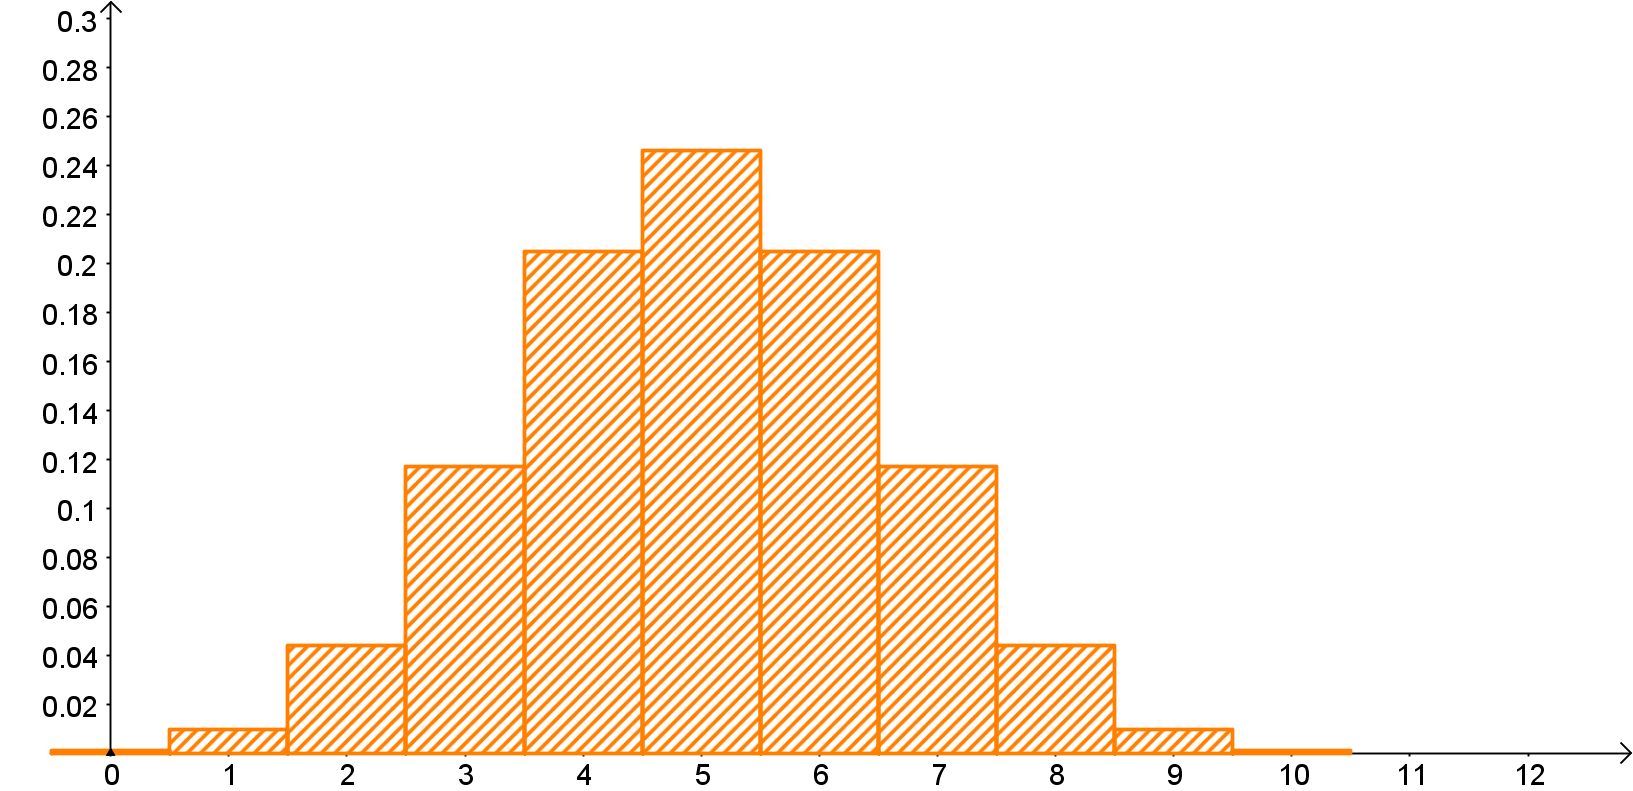
\includegraphics[width=11.5cm]{../fig/Cap05-ZooBinomial01.png}\\[3mm]
    (b)\\
    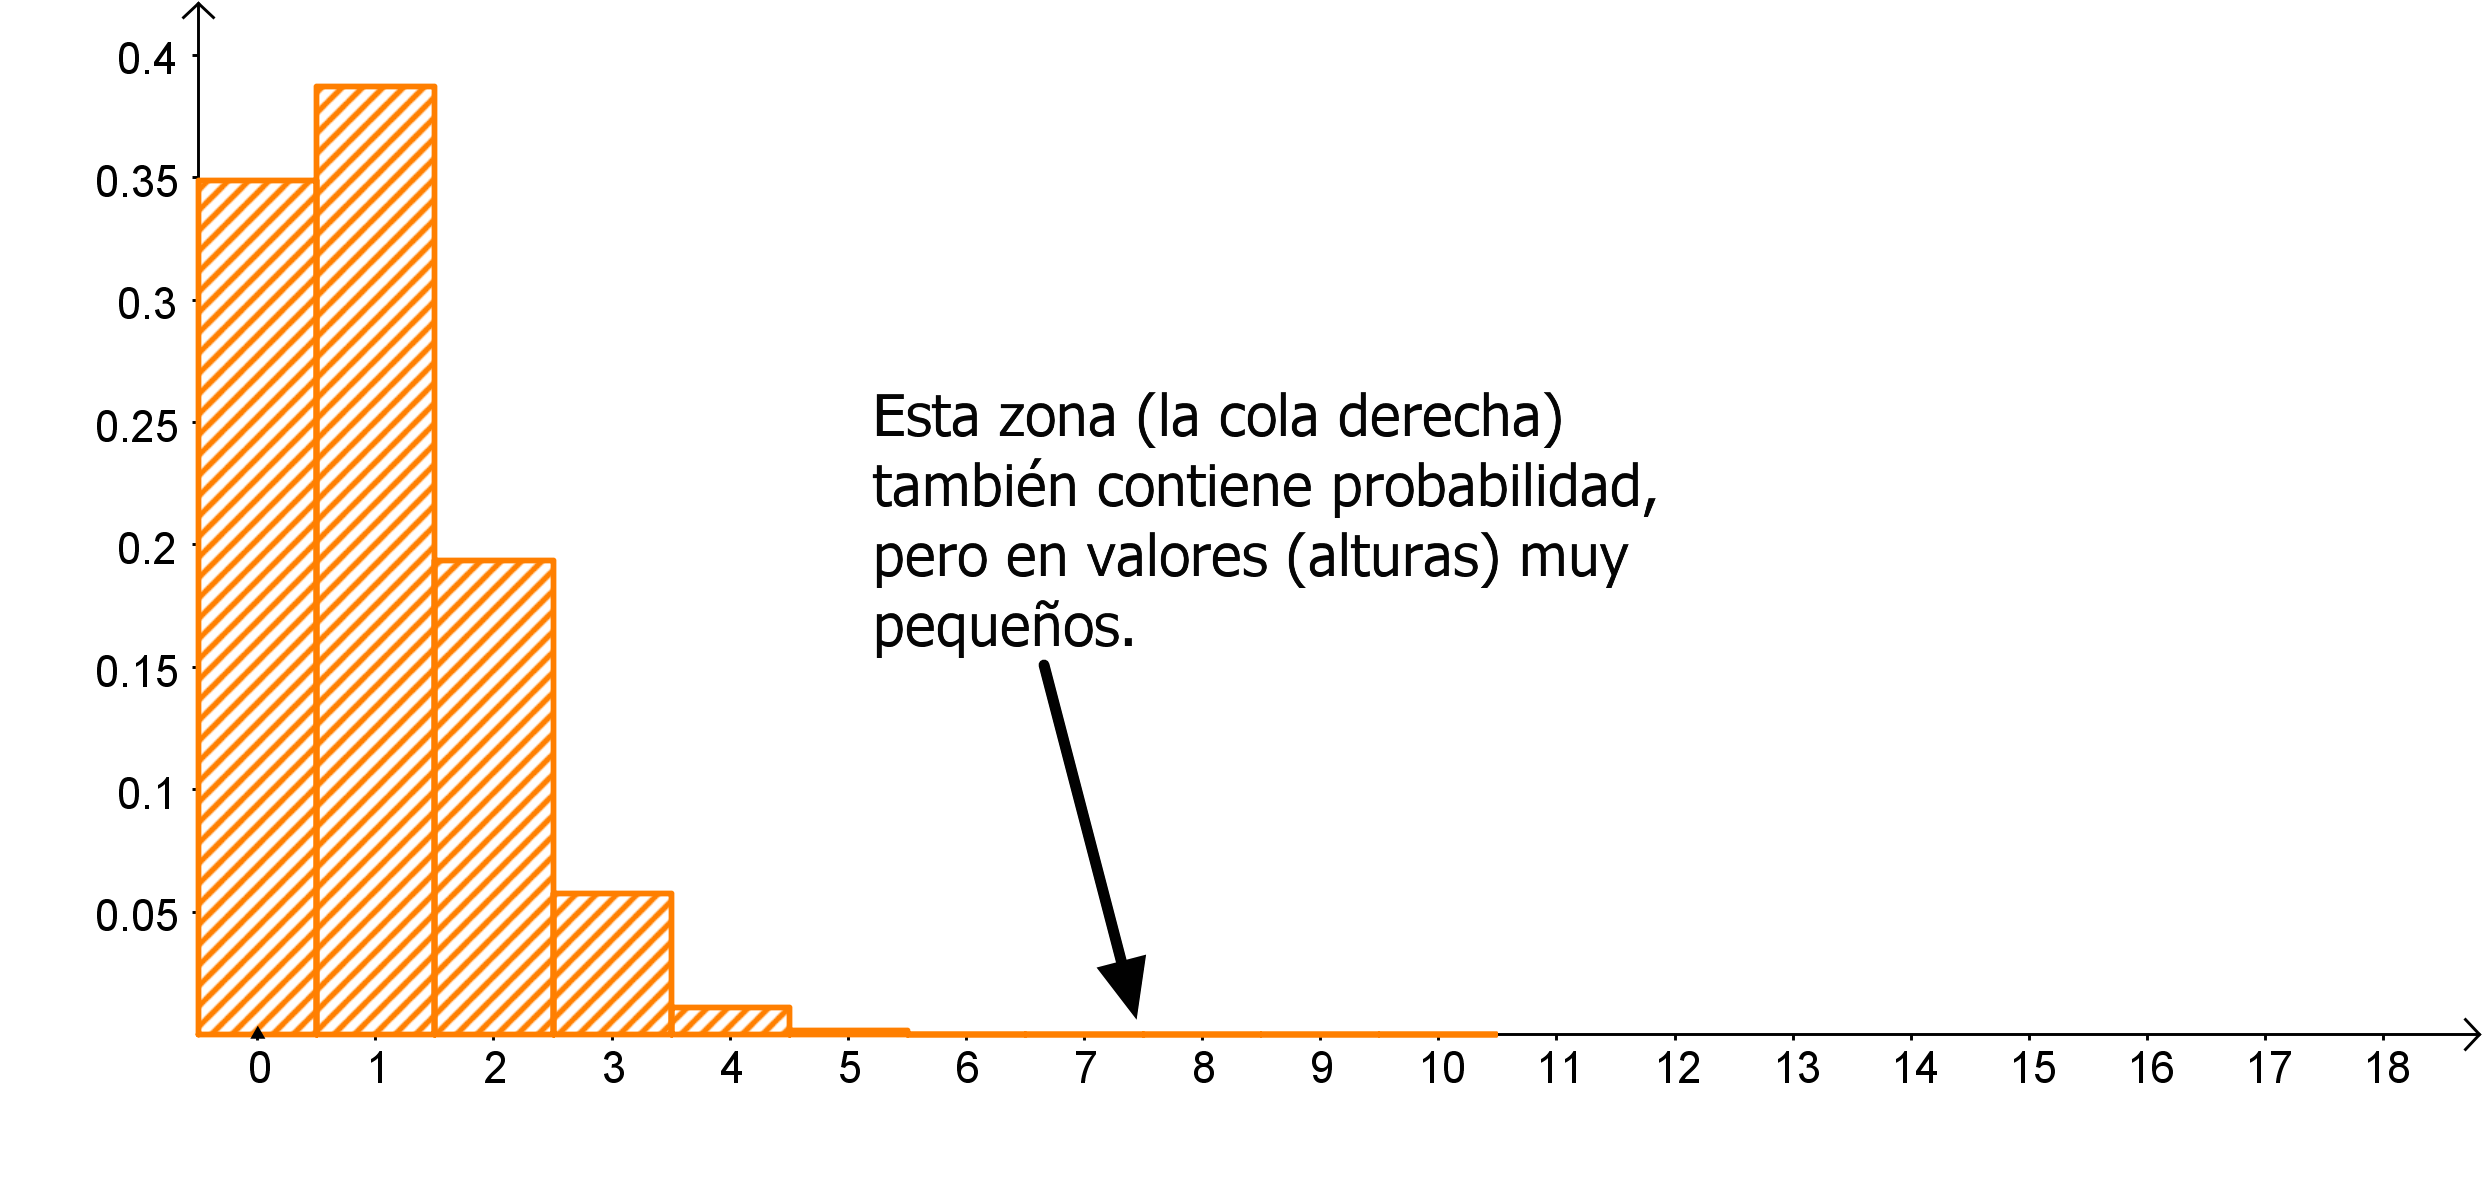
\includegraphics[width=11.5cm]{../fig/Cap05-ZooBinomial02.png}\\[3mm]
    (c)\\
    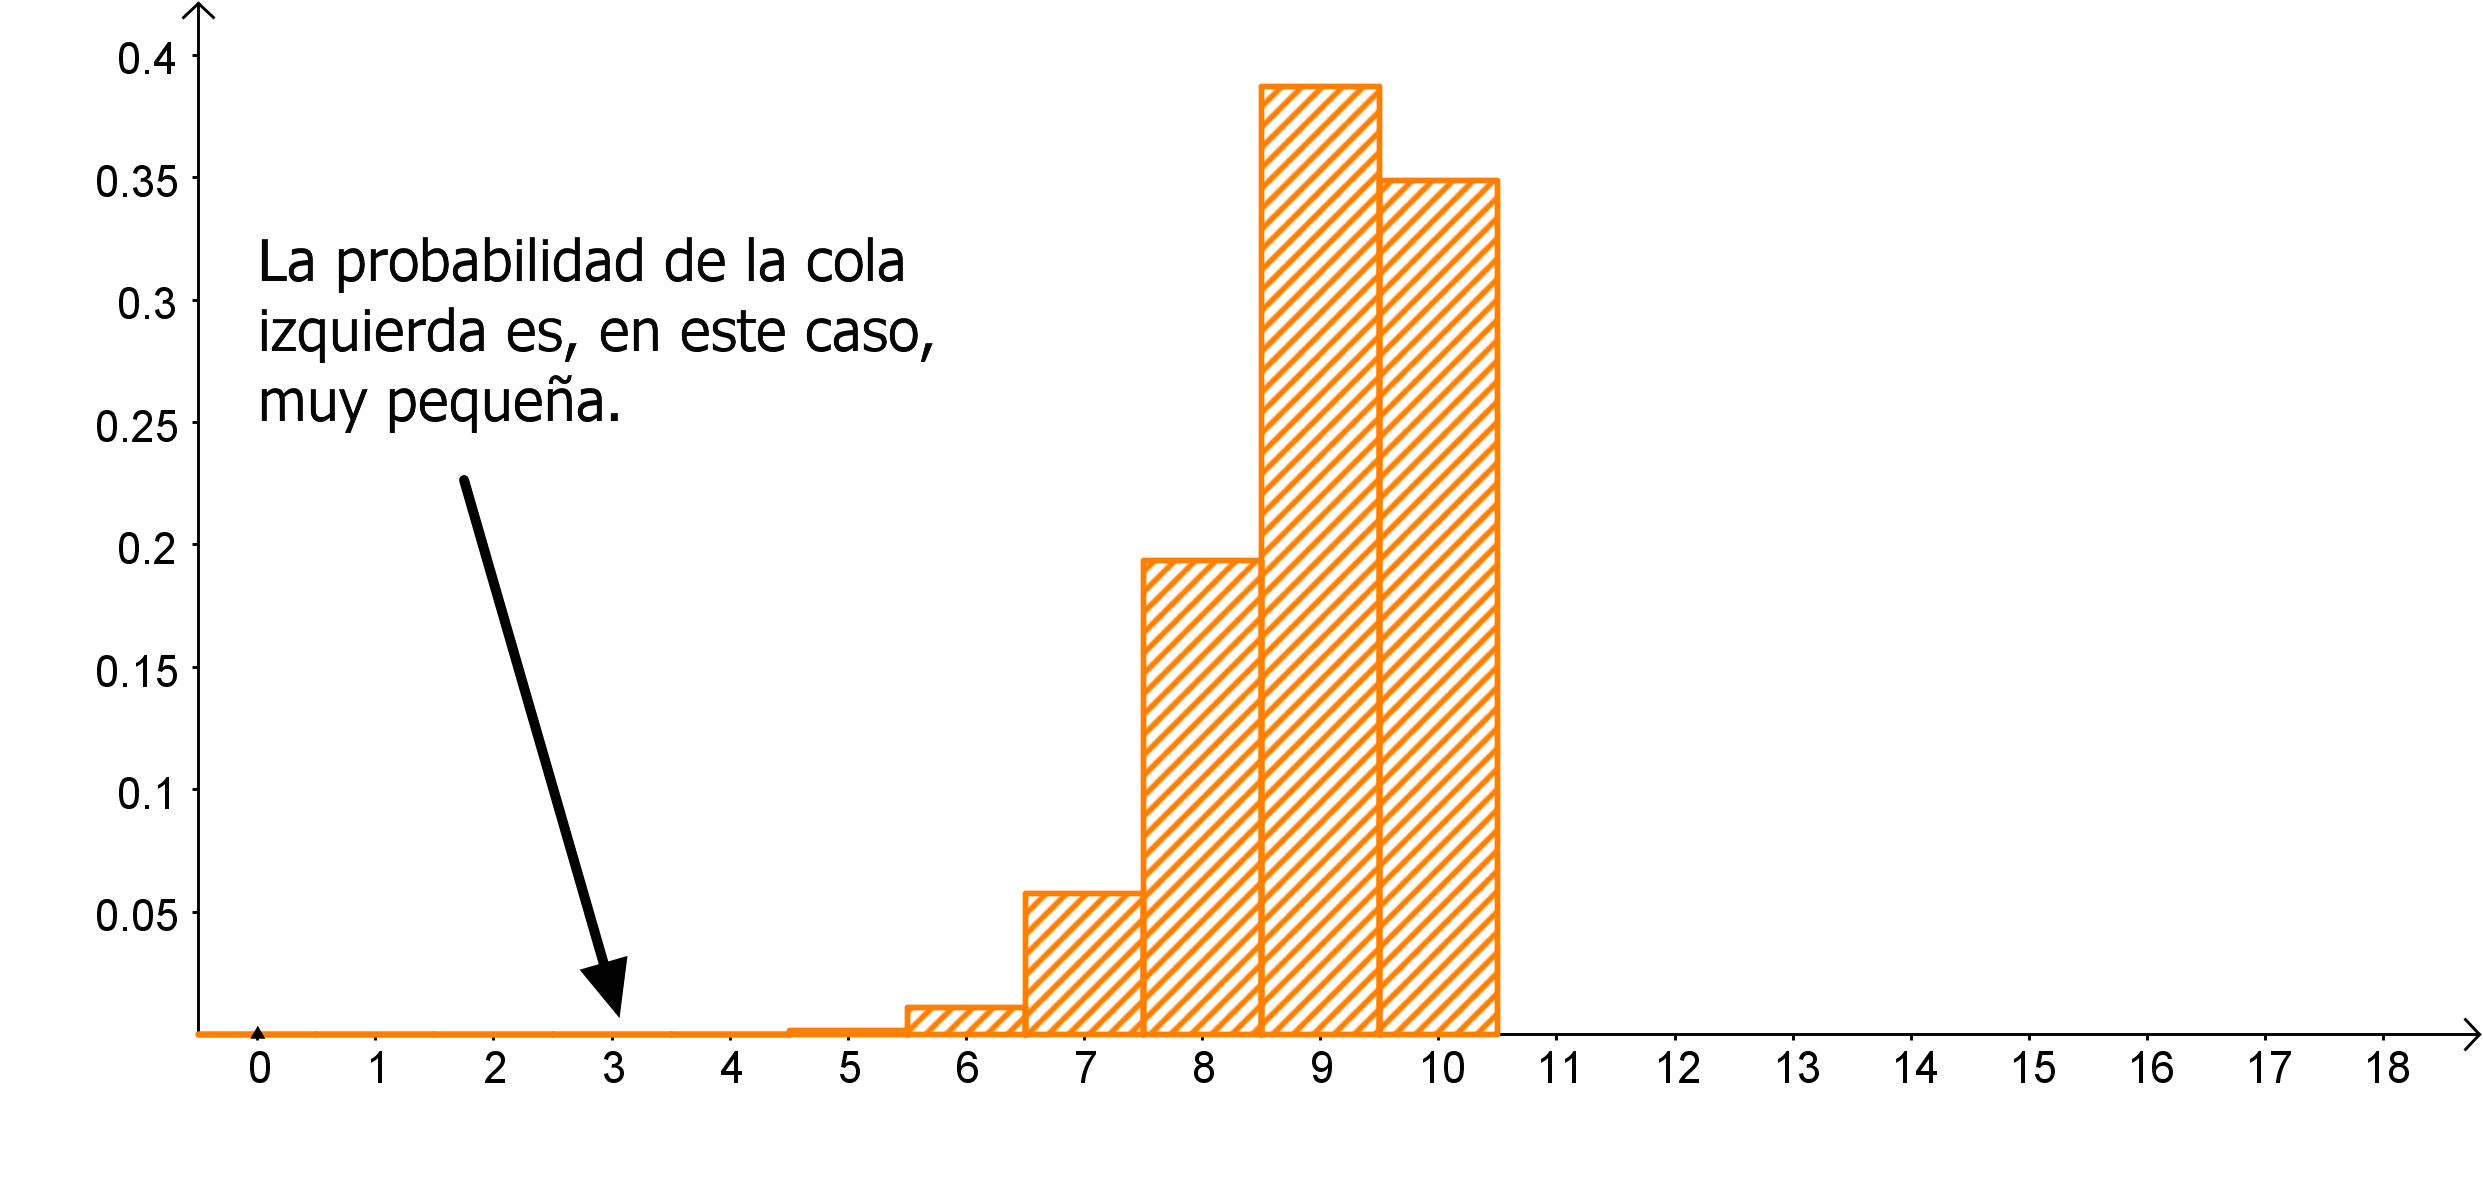
\includegraphics[width=11.5cm]{../fig/Cap05-ZooBinomial03.png}\\
	\end{enColor}
	\begin{bn}
    (a)\\
	\includegraphics[width=11.5cm]{../fig/Cap05-ZooBinomial01-bn.png}\\[3mm]
    (b)\\
    \includegraphics[width=11.5cm]{../fig/Cap05-ZooBinomial02-bn.png}\\[3mm]
    (c)\\
    \includegraphics[width=11.5cm]{../fig/Cap05-ZooBinomial03-bn.png}\\
	\end{bn}
	\caption{Distribución Binomiales: (a)  $B(10,\frac{1}{2})$.  (b) $B(10,\frac{1}{10})$.
    (c) $B(10,\frac{9}{10})$.}
	\label{cap01:fig:ZooBinomial01}
    \end{center}
  \end{figure}

En las tres binomiales de la Figura \ref{cap01:fig:ZooBinomial01} hemos mantenido un valor bastante
bajo ($n=10$) del número de ensayos. Para valores de $n$ de este tamaño, los cálculos directos con
la binomial, usando su función de densidad (Ecuación
\ref{cap05:ecu:FuncionDensidadVariableBinomial}, pág.
\pageref{cap05:ecu:FuncionDensidadVariableBinomial}), aunque resultan tediosos en extremo, se
pueden todavía hacer a mano. Pero a partir de, por decir algo, $n=50$, casi cualquier cálculo
resulta insufriblemente complicado. Y sin embargo, $n=50$ no es un número muy grande, en términos
de las posibles aplicaciones de la binomial a los problemas del mundo real. Por eso, en la próxima
sección vamos a ocuparnos de lo que sucede cuando se consideran valores de $n$ cada vez más
grandes. Como aperitivo, y siguiendo con el énfasis en la {\em forma} de la distribución podemos
invitar al lector a que eche un vistazo por adelantado a la parte (b) de la Figura
\ref{cap05:fig:HistogramaBinomial02} (pág. \pageref{cap05:fig:HistogramaBinomial02}), en la que
aparece la distribución Binomial $B(100,\frac{1}{3})$. Como decíamos, en la próxima sección vamos a
dedicarnos al estudio de las distribuciones binomiales con valores de $n$ grandes. Esencialmente,
las distribuciones binomiales se pueden agrupar, para su estudio, en estas tres posibles
situaciones:

\begin{enumerate}
  \item Binomiales con $n$ pequeño, sea cual sea el valor de $p$. En estos casos, la receta suele
      pasar por emplear directamente la función de densidad de la Ecuación Ecuación
      \ref{cap05:ecu:FuncionDensidadVariableBinomial} (pág.
      \pageref{cap05:ecu:FuncionDensidadVariableBinomial}).
  \item Binomiales con $n$ grande (ya precisaremos qué significa eso), y con valor moderado de
      $p$; ni demasiado pequeño (cercano a $0$), ni demasiado grande (cercano a $1$). Estos son
      los casos de los que nos ocuparemos en las próximas secciones.
  \item El caso restante, es aquel en el que $n$ es grande, pero los valores de $p$ son muy
      pequeños, o muy cercanos a $1$ (estos dos casos son similares, basta intercambiar los
      papeles de $p$ y $q$). Para darle al lector una idea del aspecto de las distribuciones en
      este caso, hemos representado la binomial $B(1000,\dfrac{1}{10000})$ en la Figura
      \ref{cap01:fig:ZooBinomial04}.

  \begin{figure}[hbt]
	\begin{center}
	\begin{enColor}
	\includegraphics[width=11.5cm]{../fig/Cap05-ZooBinomial04.png}
	\end{enColor}
	\begin{bn}
	\includegraphics[width=11.5cm]{../fig/Cap05-ZooBinomial04-bn.png}
	\end{bn}
	\caption{Distribución Binomial: $B\left(1000,\dfrac{1}{10000}\right)$.}
	\label{cap01:fig:ZooBinomial04}
    \end{center}
  \end{figure}


      Como puede verse, estas distribuciones son un caso extremo, que concentra casi toda la probabilidad en los valores iniciales (o finales, si $p\approx 1$), en muy pocos valores, si se comparan con $n$ (que, en este ejemplo, es $100$). Este es el caso más difícil de tratar, y de hecho lo vamos a apartar de nuestra discusión hasta la Sección \ref{cap08:sec:DistribucionPoisson} del Capítulo \ref{cap:DistribucionesRelacionadasBinomial} (pág. \pageref{cap08:sec:DistribucionPoisson}), cuando estudiaremos la distribución de Poisson, que está hecha a la medida de esta situación.
\end{enumerate}

Naturalmente, hay distribuciones que no son binomiales, y a veces basta con echar un vistazo a una gráfica de frecuencias observadas, y compararla con la gráfica teórica de probabilidades, para comprender que estamos ante una distribución que no es binomial. La Figura \ref{cap02:fig:DatosBimodales} (pág. \pageref{cap02:fig:DatosBimodales}), por ejemplo, muestra las frecuencias observadas de un conjunto de datos {\em bimodal}\index{bimodal}, con dos máximos bien diferenciados de la frecuencia. Y las distribuciones binomiales nunca son bimodales, así que la distribución de la variable, en la población de la que se ha tomado esa muestra, no parece una binomial. Una gráfica bimodal nos puede hacer sospechar que los datos que estamos observando provienen, en realidad, de la mezcla de dos poblaciones distintas, correspondientes a los dos máximos de la frecuencia.

\section{Distribuciones Binomiales con n muy grande.}\label{sec:DistribucionesBinomialesnGrande}


\noindent{\em ``If I have seen further, it is by standing upon the shoulders of giants''.\\ Isaac
Newton, 1676}.\\

Cuando los matemáticos empezaron a trabajar con la distribución binomial, no había ordenadores (ni calculadoras) disponibles. En esas condiciones, incluso el cálculo de un valor relativamente sencillo $P(X=30)$ para la distribución binomial $B(100,1/3)$, implicaba calcular números como $\binom{100}{30}$ (que es del orden de $10^{25}$). Ese cálculo podía resultar un inconveniente casi insufrible. Por esa razón, aquellos matemáticos empezaron a pensar sobre el comportamiento de la distribución binomial para valores de $n$ cada vez más grandes. Entre esos matemáticos estaba Abraham De Moivre\index{De Moivre, Abraham}, un hugonote francés refugiado en Londres, que había pasado a formar parte del selecto grupo de personas cercanas a Isaac Newton\index{Newton, Isaac}. Esa cercanía a uno de los fundadores del Cálculo nos ayuda a imaginar (sin pretensión alguna de rigor histórico) cómo pudo llegar De Moivre a algunos de sus hallazgos.

Nos imaginamos que De Moivre empezó pensando en los valores de una distribución binomial $B(n,p)$ para $n$ pequeño, por ejemplo $n=10$, y un valor cualquiera de $p$, por ejemplo $p=1/3$.
Al representar los valores de probabilidad
\[P(X=0),\quad P(X=1),\quad P(X=2),\,\ldots\,,\quad P(X=10)\]
en un gráfico similar a un histograma se obtiene la parte (a) de la Figura \ref{cap05:fig:HistogramaBinomial02} (pág. \pageref{cap05:fig:HistogramaBinomial02}). En realidad es un gráfico de columnas, pero hemos eliminado el espacio entre las columnas, por razones que enseguida serán evidentes. Fíjate en que, además, a diferencia de los histogramas del Capítulo \ref{cap:IntroduccionEstadisticaDescriptiva}, en el eje vertical estamos representando probabilidades, en lugar de frecuencias. Y, en particular, eso hace que las escalas de los ejes sean muy distintas. De Moivre, probablemente, siguió pensando en este tipo de figuras para valores de $n$ cada vez más grandes. Por ejemplo, para $n=100$ se obtiene la parte (b) de la Figura \ref{cap05:fig:HistogramaBinomial02}.

%\newpage
%\begin{figure}[t]
%\begin{center}
%\begin{enColor}
%\includegraphics[width=9cm]{../fig/Cap05-HistogramaBinomial01.png}
%\end{enColor}
%\begin{bn}
%\includegraphics[width=9cm]{../fig/Cap05-HistogramaBinomial01-bn.png}
%\end{bn}
%\caption{La distribución de probabilidad binomial $B\left(10,\frac{1}{3}\right)$.}
%\label{cap05:fig:HistogramaBinomial01}
%\end{center}
%\end{figure}
\begin{figure}[p]
\begin{center}
\begin{enColor}
\includegraphics[width=9cm]{../fig/Cap05-HistogramaBinomial01.png}\\
(a)\\
\includegraphics[width=9cm]{../fig/Cap05-HistogramaBinomial02.png}\\
(b)\\
\includegraphics[width=9cm]{../fig/Cap05-HistogramaBinomial03.png}\\
(c)
\end{enColor}
\begin{bn}
\includegraphics[width=12cm]{../fig/Cap05-HistogramaBinomial01-bn.png}\\
(a)\\
\includegraphics[width=12cm]{../fig/Cap05-HistogramaBinomial02-bn.png}\\
(b)\\
\includegraphics[width=12cm]{../fig/Cap05-HistogramaBinomial03-bn.png}\\
(c)
\end{bn}
\caption{(a) La distribución de probabilidad binomial $B\left(10,\frac{1}{3}\right)$. (b) La distribución de probabilidad binomial $B\left(100,\frac{1}{3}\right)$. (c) La misma distribución $B\left(100,\frac{1}{3}\right)$, con una curva ``misteriosa'' superpuesta.}
\label{cap05:fig:HistogramaBinomial02}
\end{center}
\end{figure}

Atención, de nuevo, a las escalas de esta Figura. En la parte (b) de esta figura la individualidad
de cada uno de los rectángulos empieza a perderse, dando paso a la percepción de una cierta forma
de {\em curva acampanada} que describe lo que ocurre, con una cima en el valor
$\mu_X=\frac{100}{3}$, como se ve en la parte (c) de la Figura
\ref{cap05:fig:HistogramaBinomial02}. ¿Cuál sería esa curva misteriosa, {\em cuál sería su
ecuación}?

Por su proximidad a Newton, estas situaciones en las que tenemos una curva y una aproximación de la
curva mediante rectángulos no le podían resultar extrañas a De Moivre. Esas mismas ideas se estaban
utilizando para sentar las bases del Cálculo Integral. En la Figura
\ref{cap05:fig:FragmentoPrincipiaNewton} hay un fragmento del libro
{\em Principia Mathematica}\index{Principia Mathematica} (páginas 42 y 44; ver el
enlace [\,\ref{enlace0009}\,]\label{enlace0009a}). Nos atrevemos a decir que es uno de
los libros más importantes en la historia de la humanidad, en el que Newton sentó las bases del
Cálculo Diferencial e Integral. En particular, uno de los problemas fundamentales que Newton
abordaba en ese libro era el del cálculo del área bajo la gráfica de una curva, lo que se denomina
la {\sf integral} de la curva. Como puedes ver, en la parte que hemos destacado, Newton sugiere que
se considere un número cada vez mayor de rectángulos bajo la curva (el número de rectángulos tiende
hacia infinito), con bases cada vez más pequeñas, en proporción al total de la figura.
\begin{figure}[bhtp]
\begin{center}
\includegraphics[height=8cm]{../fig/Cap05-NewtonPrincipia.png}
\caption{Un fragmento de los {\em Principia Mathematica} de Newton.}
\label{cap05:fig:FragmentoPrincipiaNewton}
\end{center}
\end{figure}

Esos eran exactamente los ingredientes que aparecían en la situación en la que De Moivre se
encontraba. Así que la pregunta, parecía evidente: {\em ¿cuáles serían esas curvas misteriosas  que
De Moivre estaba empezando a entrever en sus reflexiones sobre la binomial?}  Porque si tuviéramos
la ecuación de esa curva podríamos usarla para aproximar los valores de la binomial sin necesidad
de calcular los molestos números combinatorios. Por otra parte, aquellos matemáticos habían pensado
mucho sobre fórmulas binomiales, así que De Moivre consiguió identificar esas curvas, y vio que las
curvas que buscaba respondían todas a la misma fórmula. Para aproximar una distribución
binomial $B(n,p)$, con $n$ grande, y recordando que $\mu_X=np$ y $\sigma_X=\sqrt{npq}$, había que
usar la curva que ahora llamamos la {\sf curva normal}:

    \begin{center}
    \fcolorbox{black}{Gris025}{
    \begin{minipage}{8cm}
        \begin{center}
        %%%%%%%%%%%%%%%%%%%%%%%%%%%%%%%%%%%%%%%
        {\bf  Ecuación de la curva normal}
        \end{center}
        \index{normal, curva (ecuación)}\index{curva normal}
        %%%%%%%%%%%%%%%%%%%%%%%%%%%%%%%%%%%%%%%
        \begin{equation}\label{cap05:ecu:EcuacionCurvaNormal}
        f_{\mu,\sigma}(x)=\displaystyle\dfrac{1}{\sigma\sqrt{2\pi}}e^{-\frac{1}{2}\left(\frac{x-\mu}{\sigma}\right)^2}
        \quad\\[2mm]
        \end{equation}
        %%%%%%%%%%%%%%%%%%%%%%%%%%%%%%%%%%%%%%%
    \end{minipage}
    }
    \end{center}
{!`}En efecto, esos son el número $e$ y el número $\pi$! Produce un cierto vértigo verlos aparecer aquí, cuando todo esto ha empezado lanzando dados... Veamos como funciona esta fórmula en un ejemplo.
    \begin{Ejemplo}
    \label{ejem:BinomialVsNormal}
    Volvamos al cálculo que proponíamos al principio de esta sección. Calculemos $P(X=30)$ para una distribución binomial $B(100,1/3)$ (es decir, que puedes pensar que estamos tirando un dado 100 veces y preguntándonos por la probabilidad de obtener 30 veces un número 1 o 2. Probabilidad $2/6=1/3$). Si usamos la definición, calcularíamos
   \[\displaystyle
   P(X=k)=\binom{n}{k}\cdot p^k\cdot q^{n-k},
   \]
   con $n=100, k=30, p=\frac{1}{3}$. Para calcular esto hay que obtener $\binom{100}{30}\approx 2.9372\cdot 10^{25}$. Con esto, finalmente se obtiene $P(X=30)\approx 0.06728$. Si usamos la función $f_{\mu,\sigma}(x)$ con $\mu=np=\frac{100}{3}$ y $\sigma=\sqrt{n\cdot p\cdot q}\approx4.714$ se obtiene
   \[f_{\mu,\sigma}(30)\approx 0.06591.\]
   La aproximación, como vemos, no está mal, {\em aunque no es espectacular}. Hay un detalle que podría mejorarla, pero lo dejamos para más adelante, cuando hayamos entendido esto mejor.
   \quad\qed
   \end{Ejemplo}
%    Antes de seguir adelante, en \textattachfile{AproximacionBinomialPorNorrmal.R}{\textcolor{blue}{este fichero}} tienes las instrucciones en R para repetir esos cálculos.

\section{Las distribuciones continuas entran en escena...} \label{sec:distribucionesContinuasEntranEscena}

Por otra parte, regresamos a una idea que ya vislumbramos en el Capítulo \ref{cap:IntroduccionEstadisticaDescriptiva}, al hablar de datos agrupados por intervalos. Allí vimos que, al tratar con algunos conjuntos de datos,  si pensamos en valores de $n$ cada vez más grandes, las preguntas como $P(X=k)$ se vuelven cada vez menos relevantes. Si vas a lanzar un dado 10000 veces, la probabilidad de obtener exactamente $30$ veces 1 o 2 es prácticamente nula. Puedes usar el ordenador para calcularlo, como veremos en el Tutorial05. En resultado es del orden de $10^{-128}$, inimaginablemente pequeño. Incluso los valores más probables (cercanos a la media $\mu$) tienen en este ejemplo  probabilidades de en torno a $0.2$ (o un $2\%$).  No, en casos como este, lo que tiene interés es preguntar por {\em intervalos de valores}. igual que hacíamos en la Estadística Descriptiva. Es decir, nos preguntamos ¿cuál es la probabilidad de obtener 300 éxitos o menos? O también, ¿cuál es la probabilidad de obtener entre 300 y 600 éxitos del total de 1000? Para entender la respuesta, veamos algunos ejemplos.

\begin{ejemplo}
\label{cap05:ejem:DistribucionBinomialProbabilidadIntervalo01}
Volvamos por un momento a un valor de $n$ más moderado. Por ejemplo $n=21$, todavía con $p=1/3$. La media es $\mu=7$, y el diagrama correspondiente a la distribución $B(21,1/3)$ aparece en la Figura \ref{cap05:fig:HistogramaBinomial04}.
\begin{figure}[ht]
\begin{center}
\begin{enColor}
\includegraphics[width=12cm]{../fig/Cap05-HistogramaBinomial04.png}
\end{enColor}
\begin{bn}
\includegraphics[width=12cm]{../fig/Cap05-HistogramaBinomial04-bn.png}
\end{bn}
\caption{Distribución binomial $n=21$, $p=\frac{1}{3}$.}
\label{cap05:fig:HistogramaBinomial04}
\end{center}
\end{figure}
¿Cuál es la probabilidad de obtener entre 5 y 9 éxitos (ambos inclusive)? Pues la suma de áreas de los rectángulos oscuros de la Figura \ref{cap05:fig:HistogramaBinomial05} (recuerda que la suma total de áreas de los rectángulos es 1).
\begin{figure}[ht]
\begin{center}
\begin{enColor}
\includegraphics[width=12cm]{../fig/Cap05-HistogramaBinomial05.png}
\end{enColor}
\begin{bn}
\includegraphics[width=12cm]{../fig/Cap05-HistogramaBinomial05-bn.png}
\end{bn}
\caption{Probabilidad $P(5\leq X\leq 9)$ en la Distribución Binomial $B\left(21,\frac{1}{3}\right)$.}
\label{cap05:fig:HistogramaBinomial05}
\end{center}
\end{figure}
Ese valor es
\[P(5\leq X\leq 9)=P(X=5)+P(X=6)+\cdots+P(X=9),\]
y es aproximadamente $0.75$ (lo veremos en el Tutorial05). Si ahora volvemos al problema para $B(1000,1/3)$  y nos preguntamos por $P(300\leq X\leq 600)$, vemos que tendríamos que sumar el área de 301 rectángulos para calcular esa probabilidad. ¿No hay una forma mejor de hacer esto?
\qed
\end{ejemplo}

Para De Moivre, en contacto con las ideas recién nacidas sobre cálculo integral y su aplicación al cálculo del área bajo una curva, la respuesta tuvo que ser evidente. Porque precisamente Newton había descubierto que, para definir el área bajo la gráfica de una función, para valores de $x$ entre $a$ y $b$, había que considerar una aproximación del área mediante $n$ rectángulos y estudiar el límite de esas aproximaciones para $n$ cada vez más grande, como se ilustra en la Figura \ref{cap05:fig:IntegralRectangulosSumaInferior}. Para concretar, la notación (que puede intimidar un poco al principio) es esta: el área bajo la gráfica de la función\index{área bajo la gráfica de una función} $f$ en el intervalo $(a,b)$ se representa con el símbolo
\[\int_a^b f(x)dx.\]
Este símbolo se lee {\em la integral de $f$ en el intervalo $(a,b)$\index{integral de una función en un intervalo}.} No podemos, ni queremos, convertir este curso en un curso de Cálculo Integral, pero si queremos aprovechar la ocasión para que el lector\footnote{Especialmente el lector que no tiene experiencia con integrales o que sí la tiene, y ha desarrollado una cierta alergia al concepto.} tenga la oportunidad de ver, sin formalismo pero con algo de detalle, la relación que existe entre el cálculo de probabilidades de la binomial y el Cálculo Integral, porque es un ejemplo de las razones (a veces inesperadas) que hacen que los matemáticos consideren tan importante el problema de calcular áreas.
\begin{figure}[hp]
\begin{center}
\begin{enColor}
(a)\\
\includegraphics[width=12cm]{../fig/Cap05-IntegralRectangulosSumaInferior.png}\\
(b)\\
\includegraphics[width=12cm]{../fig/Cap05-IntegralRectangulosSumaInferior-a.png}
\end{enColor}
\begin{bn}
(a)\\
\includegraphics[width=12cm]{../fig/Cap05-IntegralRectangulosSumaInferior-bn.png}\\
(b)\\
\includegraphics[width=12cm]{../fig/Cap05-IntegralRectangulosSumaInferior-a-bn.png}
\end{bn}
\caption{Newton mostró como relacionar (a) el área bajo una curva (una integral) con (b) una suma de áreas de rectángulos cada vez más numerosos y estrechos.}
\label{cap05:fig:IntegralRectangulosSumaInferior}
\end{center}
\end{figure}
Y para perderle un poco el miedo al símbolo, vamos a pensar desde el lado que nos resulta más familiar, el de la suma de áreas de rectángulos. El área de un rectángulo es, naturalmente,
\[\mbox{altura}\cdot\mbox{base}.\]
Así que la suma de las áreas de los rectángulos entre $a$ y $b$ se puede escribir:
\[\sum_{\mbox{desde $a$}}^{\mbox{hasta $b$}}\left(\mbox{alturas}\cdot\mbox{bases}\right)\]
La letra griega sigma mayúscula $\displaystyle\Sigma$ que usamos en el sumatorio es el equivalente de la letra latina $S$, y se usa para representar una $\Sigma$uma. Pero si sustituyes la S griega por una S latina alargada, como este símbolo $\displaystyle\int$, verás que tienes:
\[\int_{\mbox{desde $a$}}^{\mbox{hasta $b$}}\left(\mbox{alturas}\cdot\mbox{bases}\right)\]
Y lo único que se necesita ahora es darse cuenta de que la altura de los rectángulos depende de la función $f(x)$ que estamos integrando, y el símbolo $dx$ representa la  base de esos rectángulos. Así que el símbolo de la integral tiene esta interpretación:
\[
\begin{array}{ccc}
\underbrace{\quad\int_a^b\quad}_{\mbox{\small Suma de $a$ a $b$}}&
\raisebox{-2mm}{$\underbrace{\vspace{2mm}\quad f(x)\quad}_{\mbox{\small alturas }}$}&
\raisebox{-3mm}{$\underbrace{\vspace{2mm}\quad dx\quad}_{\mbox{\small bases. }}$}
\end{array}
\]
Y animamos al lector a que recuerde siempre que, por complicada que pueda parecer, una integral está relacionada con algo sencillo, como una suma de áreas de rectángulos. La relación, más precisamente, consiste en que a medida que consideramos un número mayor de rectángulos, con bases cada vez más estrechas, las dos cantidades se van pareciendo cada vez más. En el Tutorial05 usaremos el ordenador para ilustrar de forma dinámica estas ideas.

\begin{ejemplo}
\label{cap05:ejem:DistribucionBinomialProbabilidadIntervalo02}
Vamos a volver, equipados con estas ideas, al  problema de calcular la probabilidad $P(300\leq X\leq 600)$\label{cap05:lugar:DiscusionAproximarBinomialNormal} para la distribución binomial $B(1000,1/3)$. Lo que vamos a hacer es usar
$f_{\mu,\sigma}(x)=f_{1000,1/3}(x)$, que es la curva normal que aproxima a $B(1000,1/3)$. Usando esta función, podemos aproximar la probabilidad mediante esta integral:
\[\int_{300}^{600}f_{1000,1/3}(x)dx\]
No entramos aquí en los detalles de cómo calcularla, pero el resultado es aproximadamente $0.9868$. Para comparar, y aprovechando que tenemos la suerte de disponer de ordenadores (que, por el momento, no protestan ante tareas como esta), le hemos pedido a un programa de ordenador que calcule el valor exacto, es decir que calcule:
\[P(X=300)+P(X=301)+\cdots+P(X=600).\]
usando los números combinatorios. Es decir, que calcule:
\[\sum_{k=300}^{600}\binom{1000}{k}\cdot\left(\dfrac{1}{3}\right)^k\cdot\left(\dfrac{2}{3}\right)^{1000-k}.\]
La fracción que se obtiene es, nada menos, esta:\\
$(5\-\-3\-8\-0\-1\-2\-9\-5\-1\-2\-3\-0\-2\-9\-7\-0\-7\-9\-2\-3\-4\-2\-8\-6\-0\-3\-1\-4\-3\-9\-8\-0\-7\-6\-0\-9\-3\-2\-6\-0\-9\-8\-3\-6\-6\-1\-7\-5\-4\-7\-1\-6\-8\-1\-2\-5\-3\-5\-4\-1\-9\-3\-2\-0\-3\-8\-4\-1\-7\-6\-3\-4\-3\-6\-0\-9\-4\-7\-7\-2\-3\-0\-0\-9\-6\-9\-0\-5\-5\-1\-4\-0\-4\-9\-9\-5\-2\-2\-8\-8\-0\-1\-2\-2\-1\-2\-0\-1\-5\-5\-7\-5\-6\-3\-4\-7\-8\-0\-5\-7\-2\-2\-2\-7\-0\-8\-6\-6\-8\-1\-7\-4\-7\-1\-9\-2\-2\-1\-7\-7\-0\-2\-3\-8\-4\-1\-3\-8\-8\-8\-3\-4\-0\-7\-8\-8\-6\-2\-8\-1\-8\-3\-0\-5\-2\-9\-2\-8\-2\-7\-1\-8\-9\-1\-1\-9\-1\-0\-7\-1\-0\-3\-1\-7\-8\-3\-5\-9\-3\-1\-8\-2\-6\-3\-5\-0\-4\-4\-5\-6\-0\-7\-9\-4\-2\-8\-0\-5\-1\-2\-0\-2\-5\-4\-2\-8\-7\-1\-0\-0\-5\-7\-5\-2\-0\-7\-1\-9\-0\-1\-3\-0\-2\-6\-1\-6\-3\-0\-4\-5\-3\-2\-3\-4\-7\-9\-3\-6\-4\-3\-7\-3\-1\-2\-0\-4\-3\-9\-8\-7\-4\-9\-3\-0\-2\-8\-2\-2\-0\-5\-9\-6\-4\-5\-2\-4\-8\-7\-8\-1\-9\-5\-3\-0\-9\-7\-6\-6\-6\-4\-1\-5\-5\-8\-1\-3\-2\-8\-3\-8\-9\-6\-1\-9\-2\-4\-4\-4\-6\-6\-9\-9\-7\-0\-9\-9\-1\-6\-0\-0\-5\-0\-9\-1\-8\-4\-4\-2\-4\-4\-2\-9\-9\-4\-7\-0\-9\-6\-4\-6\-5\-3\-6\-9\-4\-6\-8\-5\-5\-0\-6\-9\-4\-7\-5\-8\-8\-7\-0\-9\-1\-2\-5\-0\-1\-2\-6\-1\-0\-3\-8\-1\-7\-6\-2\-8\-8\-8\-7\-4\-2\-2\-3\-8\-3\-8\-2\-3\-3\-5\-6\-3\-6\-4\-7\-3\-4\-9\-0\-0\-0\-4\-2\-5\-9\-7\-7\-7\-7\-8\-8\-4\-7\-3\-4\-4\-5\-4\-3\-9\-1\-7\-7\-7\-9\-7\-7\-7\-0\-6\-6\-6\-9\-8\-3\-1\-9\-3\-4\-5\-5\-5\-1\-3\-1\-0\-9\-7\-6\-9\-6\-7\-9\-6\-1\-8\-7\-4\-8\-7\-8\-4\-3\-3\-7\-1\-2\-3\-4\-3\-6\-1\-3\-4\-4\-)\,/\,(5\-4\-4\-0\-6\-2\-0\-6\-5\-6\-2\-9\-9\-6\-1\-5\-7\-8\-9\-6\-7\-2\-6\-5\-5\-3\-8\-9\-9\-2\-6\-5\-2\-0\-0\-2\-4\-5\-4\-9\-0\-6\-1\-8\-6\-3\-1\-7\-7\-5\-6\-4\-4\-7\-5\-9\-8\-7\-3\-2\-6\-6\-1\-8\-2\-1\-7\-4\-0\-1\-6\-3\-5\-1\-7\-1\-6\-2\-5\-1\-0\-0\-9\-9\-0\-8\-5\-7\-2\-5\-8\-6\-4\-4\-4\-7\-7\-6\-2\-1\-2\-5\-0\-6\-5\-7\-5\-2\-1\-3\-8\-6\-3\-0\-6\-9\-2\-3\-2\-7\-5\-5\-1\-8\-3\-3\-1\-6\-1\-3\-5\-8\-2\-7\-9\-3\-8\-7\-5\-9\-8\-9\-0\-6\-4\-7\-1\-2\-9\-9\-5\-6\-9\-4\-1\-3\-1\-8\-0\-0\-9\-0\-6\-2\-7\-6\-5\-3\-6\-2\-9\-9\-6\-0\-4\-4\-3\-6\-2\-7\-4\-7\-9\-1\-0\-6\-5\-6\-9\-8\-9\-3\-5\-2\-8\-5\-5\-5\-7\-2\-0\-2\-1\-2\-9\-9\-9\-4\-3\-1\-2\-9\-2\-6\-4\-5\-6\-5\-7\-5\-3\-7\-2\-9\-3\-4\-5\-4\-5\-0\-1\-2\-5\-9\-9\-0\-3\-7\-7\-4\-9\-1\-9\-3\-7\-7\-2\-3\-2\-3\-0\-0\-6\-1\-9\-8\-2\-6\-3\-8\-9\-0\-8\-6\-5\-6\-1\-4\-8\-3\-7\-6\-4\-2\-1\-9\-9\-1\-6\-4\-7\-6\-9\-1\-1\-8\-5\-9\-0\-3\-9\-2\-4\-6\-1\-9\-5\-4\-3\-8\-7\-3\-9\-1\-8\-5\-5\-2\-6\-8\-5\-9\-4\-9\-1\-2\-6\-6\-9\-0\-6\-2\-9\-2\-2\-7\-5\-0\-6\-8\-4\-7\-6\-6\-6\-9\-9\-1\-2\-7\-1\-4\-7\-8\-1\-2\-9\-8\-9\-3\-1\-7\-2\-2\-1\-8\-0\-6\-3\-2\-7\-6\-1\-0\-5\-8\-9\-4\-7\-3\-9\-5\-8\-2\-1\-5\-4\-7\-2\-9\-9\-8\-7\-4\-6\-9\-8\-2\-5\-7\-2\-0\-9\-4\-4\-0\-5\-7\-1\-2\-3\-8\-2\-9\-6\-4\-7\-1\-6\-4\-1\-8\-4\-0\-0\-9\-8\-2\-9\-7\-9\-8\-4\-6\-9\-7\-2\-6\-3\-5\-3\-3\-1\-8\-8\-7\-8\-4\-8\-4\-1\-9\-0\-6\-1\-7\-7\-2\-0\-7\-5\-5\-8\-0\-7\-9\-0\-8\-3\-5\-8\-1\-3\-8\-6\-3\-7\-9\-7\-7\-5\-8\-1\-0\-7\-)$ \\
que es aproximadamente $0.9889$ (con cuatro cifras significativas).
\qed
\end{ejemplo}
Hemos incluido la fracción completa (que es reducida, sin factores comunes a numerador y denominador) para que el lector tenga ocasión de ponderar la situación pausadamente. Es cierto, sobre todo para alguien que comienza el estudio de la Estadística, que cambiar una suma por una integral puede parecer una complicación innecesaria. {!`}Pero, como demuestra esa fracción, no hablamos de una suma cualquiera! El esfuerzo computacional que supone hallar esa fracción es muy superior al de calcular el valor de la integral, de manera que, hasta hace muy pocos años, era imposible, en la práctica, obtener ese valor exacto. Insistimos, porque creemos que es esencial que se entienda esto: frente al cálculo directo de los valores de la Binomial, {\em la integral de la curva normal es un atajo, es el cámino más cómodo}. Y si se tiene en cuenta que el valor exacto es $0.9889$, y que la aproximación de la curva normal es $0.9868$, el atajo funciona bastante bien (sobre todo, desde la perspectiva previa a los ordenadores).

%De hecho, si usamos R para sumar los valores $P(X=300)+\cdots+P(X=600)$ se obtiene aproximadamente $0.9888$. La aproximación está muy bien, y eso que aún tenemos pendiente mejorar el ajuste de la curva $f_{\mu,\sigma}(x)$ con los valores de $B(p,n)$.

Recapitulemos: para calcular la probabilidad $P(a\leq X\leq b)$ de $B(n,p)$ hemos usado una cierta función $f_{\mu,\sigma}(x)$, y hemos visto que
    \[P(a\leq X\leq b)\approx \int_a^b f_{\mu,\sigma}(x)dx.\]
Las ideas que subyacen a la aproximación de la Distribución Binomial por la normal son muy importantes; de hecho, son en algún sentido uno de los hallazgos más importante de toda la historia de la Estadística (y, sin temor a exagerar, de toda la historia de la Ciencia). Pero no es la única aproximación de ese estilo que encontraron los matemáticos. Y a medida que se acostumbraban a estas ideas, y empezaban a pensar en el lado derecho de esa aproximación, se dieron cuenta de que esas integrales constituían, por si mismas, una forma de repartir o {\em distribuir} la probabilidad, muy similar a lo que hemos aprendido a hacer con las tablas de las variables aleatorias discretas (como la Tabla \ref{cap04:tabla:tablaDensidadProbabilidadGenericaVariableAleatoriaDiscreta}, pág. \pageref{cap04:tabla:tablaDensidadProbabilidadGenericaVariableAleatoriaDiscreta}). Sólo que aquí, a diferencia de lo que ocurre en esas Tablas, no hay una {\em lista discreta} de valores, sino un {\em intervalo continuo}. La palabra clave aquí es {\em continuo}. De hecho, hemos dejado pendiente desde la Sección \ref{sec:variablesAletorias} (pág. \pageref{sec:variablesAletorias}) el tratamiento general de las variables aleatorias continuas. En el próximo apartado retomamos esa discusión, a la luz de lo que hemos aprendido. Cuando hayamos profundizado en esto, y hayamos extendido nuestro vocabulario, volveremos al tema de la aproximación de la Distribución Binomial.

\section{Función de densidad, media y varianza de una variable continua.}
\label{cap05:sec:MasDetallesSobreDistribucionesContinuas}

La idea con la que hemos cerrado el apartado anterior es que se puede usar una integral para asignar valores de probabilidad. En esta sección vamos a ver cómo se hace esto con, inevitablemente, bastantes más detalles técnicos. Pero tratando, como siempre, de no enredarnos en el formalismo y apoyarnos en el ordenador todo lo que nos sea posible. No te asustes si nunca has calculado una integral. El ordenador calculará por nosotros. Tampoco calculamos ``a mano'' nunca un logaritmo (salvo los más elementales), y nos hemos acostumbrado a que las máquinas se encarguen de esa tarea. Naturalmente, cuanto más aprendas sobre las {\em propiedades} de las integrales, tanto mejor. Pero queremos distinguir entre las propiedades y el cálculo, porque son cosas distintas (como sucede, de nuevo, en el caso de los logaritmos).

Como hemos dicho al cerrar la anterior sección, en una variable discreta, que toma una cantidad
finita de valores, utilizamos  una tabla como la Tabla
\ref{cap04:tabla:tablaDensidadProbabilidadGenericaVariableAleatoriaDiscreta}, pág.
\pageref{cap04:tabla:tablaDensidadProbabilidadGenericaVariableAleatoriaDiscreta}) para repartir la
probabilidad entre los distintos valores. Pero con una variable aleatoria, que toma infinitos
valores (todos los valores de un intervalo), no podemos hacer eso. Si la variable aleatoria
continua $X$ toma todos los valores del intervalo $(a,b)$, vamos a aprender a utilizar las
integrales, para repartir la probabilidad entre esos valores. En el siguiente cuadro se resume la
información esencial, que a continuación vamos a explorar con detenimiento.
    \begin{center}
    \fcolorbox{black}{Gris025}{
    \begin{minipage}{12cm}
        \begin{center}
        %%%%%%%%%%%%%%%%%%%%%%%%%%%%%%%%%%%%%%%
        {\bf  Función de densidad de una variable aleatoria continua}
        \end{center}
        \index{variable aleatoria continua y su función de densidad}
        %%%%%%%%%%%%%%%%%%%%%%%%%%%%%%%%%%%%%%%
        Para definir una variable aleatoria continua $X$, que tome valores en $(-\infty,\infty)$  podemos utilizar una {\sf función de densidad}, que es una función $f(x)$ que tiene estas propiedades:
        \begin{itemize}
        \item[(a)] No negativa: $f(x)\geq 0$ para todo $x$; es decir, $f$ no toma valores negativos.
        \item[(b)] Probabilidad total igual a $1$: el área total bajo la gráfica de $f$ es 1:
        \[\int_{-\infty}^{\infty}f(x)dx=1\]
        \end{itemize}
        %%%%%%%%%%%%%%%%%%%%%%%%%%%%%%%%%%%%%%%
    \end{minipage}}
    \end{center}
Entonces, la función de densidad permite calcular probabilidades asociadas a $X$ mediante esta igualdad básica:
    \begin{center}
    \fcolorbox{black}{Gris025}{
    \begin{minipage}{12cm}
        \begin{center}
        %%%%%%%%%%%%%%%%%%%%%%%%%%%%%%%%%%%%%%%
        {\bf  Probabilidad de un intervalo, usando la  función de densidad de una variable aleatoria continua.}
        \end{center}
        %%%%%%%%%%%%%%%%%%%%%%%%%%%%%%%%%%%%%%%
        Para calcular la probabilidad de que $X$ tome valores en el intervalo $(a,b)$, integramos su función de densidad en ese intervalo:
        \begin{equation}\label{cap05:ecu:AsignacionProbabilidadIntegralDensidad}
        P(a\leq X\leq b)=\int_a^b f(x)dx.
        \end{equation}
        %%%%%%%%%%%%%%%%%%%%%%%%%%%%%%%%%%%%%%%
    \end{minipage}}
    \end{center}


No te preocupes si ahora mismo no entiendes como usar esto. {!`}Y una vez más, sobre todo, no te dejes intimidar por las integrales! Enseguida veremos ejemplos, y quedará todo más claro. Pero antes de seguir adelante, queremos hacer un par de comentarios:
\begin{enumerate}
  \item El intervalo $(a,b)$ de valores de la variable puede ser, en muchos casos, un intervalo sencillo, como $(0,10)$. Pero también nos vamos a encontrar con ejemplos donde el intervalo es no acotado, como por ejemplo $(0,+\infty)$, en el caso de una variable aleatoria que pueda tomar como valor cualquier número real positivo. Y hay, desde luego, casos más complicados, como por ejemplo, una variable aleatoria que pueda tomar valores en {\em la unión} de intervalos $(0,7) \cup (12,19)$. Nosotros vamos a empezar explicando el caso del intervalo $(-\infty,\infty)$, que es como decir que suponemos que la variable $X$ puede, en principio, tomar cualquier valor. Y más adelante explicaremos lo que hay que hacer en otros casos.
  \item La integral se diseñó, en su origen, para tratar el problema del cálculo de áreas. Nosotros, ahora, estamos empezando a usar integrales para calcular probabilidades. Esto, sin embargo, no debería resultar una sorpresa. En la Sección \ref{cap03:sec:ProbabilidadMasAllaReglaLaplace} (pág. \pageref{cap03:sec:ProbabilidadMasAllaReglaLaplace}) presentamos varios ejemplos de problemas de lo que llamábamos Probabilidad Geométrica, con los que tratamos de hacer ver la íntima conexión que existe entre los conceptos de área y de probabilidad. Los resultados que vamos a ver en este capítulo son el primer paso para abordar esos problemas de Probabilidad Geométrica. Pero debemos prevenir al lector de que el análisis detallado de muchos de esos problemas de Probabilidad Geométrica requiere un dominio del Cálculo Integral que va más allá de lo que estamos dispuestos a asumir (entre otras cosas, porque implica tareas que el ordenador no puede hacer por nosotros).
\end{enumerate}

Vamos a empezar con un ejemplo que ilustre la definición de función de densidad de una variable aleatoria continua.
\begin{ejemplo}[Cálculo de la probabilidad de un intervalo, integrando una función de densidad. Primera parte]
\label{cap05:ejem:CalculoProbabilidadIntegralParte1}
    Vamos a definir una variable aleatoria continua $X$ usando como función de densidad:
    \[f(x)=\dfrac{1}{\pi(1+x^2)}.\]
    La gráfica de esta función se muestra en la Figura \ref{cap05:fig:DistribucionCauchy}.
\begin{figure}[hp]
\begin{center}
\begin{enColor}
\includegraphics[width=12cm]{../fig/Cap05-DistribucionCauchy.png}\\
\end{enColor}
\begin{bn}
\includegraphics[width=12cm]{../fig/Cap05-DistribucionCauchy-bn.png}
\end{bn}
\caption{Un ejemplo de función de densidad para una variable aleatoria continua.}
\label{cap05:fig:DistribucionCauchy}
\end{center}
\end{figure}

    Hemos querido empezar con esta función porque es un ejemplo suficientemente sencillo, en el que el lector podrá ver el tipo de recursos que vamos a necesitar, pero a la vez no es engañosamente simple. En el Tutorial05 veremos cómo comprobar que esta función de densidad satisface la propiedad (b), que debe satisfacer cualquier función de densidad para ser digna de ese nombre. Aquí queremos centrarnos en aprender a utilizar esta función para calcular la probabilidad de un cierto intervalo. Por ejemplo, vamos a calcular
    \[P(0\leq X\leq 1)\]
    para esta variable aleatoria continua. Sabemos, por la Ecuación \ref{cap05:ecu:AsignacionProbabilidadIntegralDensidad}, que la forma de asignar la probabilidad a un intervalo es mediante la integral:
    \[P(a\leq X\leq b)=\int_a^b f(x)dx.\]
    En este ejemplo $(a,b)=(0,1)$, y $f(x)=\frac{1}{\pi(1+x^2)}$. Así que eso significa que debemos calcular esta integral:
    \[
    P(0\leq X\leq 1)=\int_0^1f(x)dx=\int_0^1\dfrac{1}{\pi(1+x^2)}dx,
    \]
    o, lo que es lo mismo, que tenemos que calcular el área sombreada de la Figura \ref{cap05:fig:DistribucionCauchy-2}. Vamos a introducir más terminología, y a dar algunos detalles técnicos, antes de retomar el ejemplo.
    \qed

\begin{figure}[htbp]
\begin{center}
\begin{enColor}
\includegraphics[width=12cm]{../fig/Cap05-DistribucionCauchy-2.png}
\end{enColor}
\begin{bn}
\includegraphics[width=12cm]{../fig/Cap05-DistribucionCauchy-2-bn.png}
\end{bn}
\caption{La probabilidad $P(0\leq X\leq 1)$ se calcula integrando $f(x)$ entre $0$ y $1$.}
\label{cap05:fig:DistribucionCauchy-2}
\end{center}
\end{figure}

\end{ejemplo}
¿Cómo se calcula la integral que ha aparecido en este ejemplo? En la inmensa mayoría de los casos, cuando se desea un resultado exacto (simbólico), el cálculo es un proceso en dos pasos, usando el método que se conoce como {\sf Teorema Fundamental del Cálculo Integral}\index{teorema fundamental del cálculo integral} (o Regla de Barrow)\index{regla de Barrow}:
    \begin{center}
    \fcolorbox{black}{Gris025}{
    \begin{minipage}{12cm}
        \begin{center}
        %%%%%%%%%%%%%%%%%%%%%%%%%%%%%%%%%%%%%%%
        {\bf Teorema Fundamental del Cálculo Integral}
        \index{teorema fundamental del cálculo integral}
        \end{center}
        %%%%%%%%%%%%%%%%%%%%%%%%%%%%%%%%%%%%%%%
        \begin{enumerate}
          \item Buscamos una función $F(x)$ que cumpla $F'(x)=f(x)$. Esa función $F$ se denomina una {\sf primitiva}\index{primitiva} de $f(x)$, también se representa mediante el símbolo de integral, pero sin que aparezcan los extremos del intervalo:
              \[F(x)=\int f(x)dx.\]
              La notación habitual para una primitiva es, como hemos hecho aquí, utilizar la misma letra pero en mayúsculas.
          \item Una vez que hemos hallado $F$, la integral (es decir, el área, es decir, la probabilidad) es igual a la diferencia de valores de $F$ en los extremos del intervalo:
              \begin{equation}\label{cap05:ecu:TeoremaFundamentalCalculo}
              \int_a^b f(x)dx = F(b)-F(a).
              \end{equation}
        \end{enumerate}
        %%%%%%%%%%%%%%%%%%%%%%%%%%%%%%%%%%%%%%%
    \end{minipage}}
    \end{center}
Como puede verse, este método descansa sobre nuestra capacidad de calcular una primitiva de $F$. Esa operación puede ser muy difícil, o incluso imposible en algunos casos (volveremos sobre esto). Y tradicionalmente, los estudios de Matemáticas consagraban mucho tiempo y esfuerzo a aprender los métodos para encontrar primitivas. Afortunadamente, en la segunda mitad del siglo XX esa tarea se ha mecanizado, y ahora podemos dejar que los ordenadores se encarguen del trabajo más tedioso. Existen muchos programas, accesibles incluso mediante páginas web, desde un teléfono móvil, que calculan primitivas en todos los casos que vamos a necesitar. En el Tutorial05 veremos varios de estos programas, y practicaremos su uso. Volvamos al ejemplo.
\begin{ejemplo}[Continuación del Ejemplo \ref{cap05:ejem:CalculoProbabilidadIntegralParte1}]
\label{cap05:ejem:CalculoProbabilidadIntegralParte2}
Usando alguno de los recursos que conoceremos en el Tutorial05, obtenemos una primitiva de $f(x)=\frac{1}{\pi(1+x^2)}$. El resultado es:
\[F(x)=\int f(x)dx=\int \frac{1}{\pi(1+x^2)} dx = \dfrac{1}{\pi}\arctan x.\]
Eso significa que si calculas la derivada de
\[F(x)=\dfrac{1}{\pi}\arctan x,\]
el resultado tiene que ser $f(x)$, la función de densidad (si sabes suficiente de derivación, que es mucho más fácil que la integración, siempre puedes (debes) comprobar a mano este tipo de afirmaciones).

Ahora podemos usar esta primitiva para calcular la probabilidad:
    \[
    P(0\leq X\leq 1)=\int_0^1f(x)dx=F(1)-F(0)=\]
    \[\left(\dfrac{1}{\pi}\arctan 1\right)-\left(\dfrac{1}{\pi}\arctan 0\right)=\dfrac{1}{4}-0=\dfrac{1}{4}
    \]
Así que la probabilidad que buscábamos es $\dfrac{1}{4}$.
\qed
\end{ejemplo}
En este ejemplo hemos puesto el énfasis en el cálculo de primitivas para que el lector pueda entender el método con algo más de detalle. Pero los mismos programas que calculan primitivas permiten calcular la integral
\[\int_0^1\dfrac{1}{\pi(1+x^2)}dx\]
en un sólo paso. De nuevo, nos remitimos al Tutorial05, donde veremos con más detalle las dos formas de proceder. Dejamos al lector la tarea de usar uno de estos programas para comprobar que la función de densidad del ejemplo cumple la propiedad (b) de las funciones de densidad (ver la página \pageref{cap05:ecu:AsignacionProbabilidadIntegralDensidad}). Esa propiedad garantiza que la probabilidad total es 1, y eso, como sabemos, es una de las Propiedades Fundamentales de la Probabilidad (pág. \pageref{cap03:def:PropiedadesFundamentalesFuncionProbabilidad}). Nosotros vamos a hacer esa comprobación usando la primitiva que hemos hallado, para así tener la ocasión de discutir algunos aspectos adicionales.

Antes de eso, un consejo, a modo de advertencia, dirigido a aquellos lectores con menos entrenamiento matemático. Sabemos que algunos de estos ejemplos, usando integrales y otros recursos técnicos, pueden resultar difíciles de digerir al principio. El consejo es que no hay que quedarse atascado en ellos. Las integrales nos sirven, simplemente, para hacer cálculos relacionados con probabilidades en variables continuas. Si ahora no entiendes algún ejemplo, trata sólo de captar la idea general, que suele estar más o menos clara, y sigue adelante. Con la práctica, después de ver varios casos, y hacer algunos ejercicios, las cosas irán quedando más claras, y podrás volver a leer el ejemplo que se te atragantó. Seguramente, lo entenderás mejor. Pero si, finalmente, no es así, asegúrate de pedir ayuda a alguien que sepa más de Matemáticas.
\begin{ejemplo}
\label{cap05:ejem:DistribucionCauchyIntegralTotal1}
    Vamos a utilizar la primitiva que hemos hallado en el Ejemplo \ref{cap05:ejem:CalculoProbabilidadIntegralParte2}, para comprobar que se cumple
    \[\int_{-\infty}^{\infty}\dfrac{1}{\pi(1+x^2)}dx=1.\]
    Nos vamos a detener en esto, porque queremos que el lector compruebe que, en muchos casos, la presencia del símbolo $\infty$ no supone ninguna complicación excesiva. Procedemos como en el Ejemplo \ref{cap05:ejem:CalculoProbabilidadIntegralParte2}. Tenemos la primitiva:
    \[F(x)=\int f(x)dx=\int \frac{1}{\pi(1+x^2)} dx = \dfrac{1}{\pi}\arctan x.\]
    Y usando el Teorema Fundamental del Cálculo obtenemos:
    \[\int_{-\infty}^{\infty}\dfrac{1}{\pi(1+x^2)}dx=F(\infty)-F(-\infty).\]
    ¿Qué significa $F(\infty)$? Sustituyendo ingenuamente, como si infinito fuera un número cualquiera, obtenemos
    \[\dfrac{1}{\pi}\arctan(\infty).\]
    Así que la pregunta pasa a ser ``¿qué significa $\arctan(\infty)$?''. La respuesta técnica es que tendríamos que calcular un límite. Pero en este, y en muchos otros casos, podemos tomar un camino más sencillo. Cuando un matemático ve un símbolo como $\infty$, sabe que casi siempre eso significa que debemos preguntarnos lo que sucede cuando pensamos en valores muy grandes de la variable; de hecho, tan grandes como se quiera. Vamos a representar la gráfica de la función $F(x)$, que puede verse en la Figura \ref{cap05:fig:Cap05-GraficaArcoTangente}.

\begin{figure}[htbp]
\begin{center}
\begin{enColor}
\includegraphics[width=12cm]{../fig/Cap05-GraficaArcoTangente.png}
\end{enColor}
\begin{bn}
\includegraphics[width=12cm]{../fig/Cap05-GraficaArcoTangente-bn.png}
\end{bn}
\caption{Gráfica de la función $F(x)$ del Ejemplo \ref{cap05:ejem:DistribucionCauchyIntegralTotal1}.}
\label{cap05:fig:Cap05-GraficaArcoTangente}
\end{center}
\end{figure}

    Hemos añadido dos líneas de trazos a esa figura para hacer ver que, para valores muy grandes de $x$, de hecho, cuanto más grande sea $x$, más se parece el valor de $\arctan(x)$ a $\dfrac{\pi}{2}$. Así que podemos decir, sin temor a equivocarnos, que
    \[\arctan(\infty)=\dfrac{\pi}{2}.\]
    Y de la misma forma:
    \[\arctan(-\infty)=-\dfrac{\pi}{2}.\]
    Por lo tanto, la integral (de probabilidad total) que tratábamos de calcular es (atención al $1/\pi$ en $F$):
    \[\int_{-\infty}^{\infty}\dfrac{1}{\pi(1+x^2)}dx=F(\infty)-F(-\infty)=\]
    \[\dfrac{1}{\pi}\arctan(\infty)-\dfrac{1}{\pi}\arctan(-\infty)=
    \dfrac{1}{\pi}\left(\dfrac{\pi}{2}\right)-\dfrac{1}{\pi}\left(-\dfrac{\pi}{2}\right)=1.\]
    \qed
\end{ejemplo}
Esta propiedad de las funciones de densidad, el hecho de que la integral total vale 1, nos será de mucha utilidad para ahorrarnos algunos cálculos. El siguiente ejemplo pretende ilustrar esto:
\begin{ejemplo}\label{cap05:ejem:DistribucionCauchyTrucosProbabilidad}
    Todavía con la función del Ejemplo \ref{cap05:ejem:CalculoProbabilidadIntegralParte1}, vamos a calcular la probabilidad:
    \[
    P(X>1)=\int_1^{\infty}f(x)dx
    \]
    Es decir, el área sombreada de la Figura \ref{cap05:fig:Cap05-DistribucionCauchy-IntegralColaDerecha}. Se trata de un intervalo {\em no acotado}, que se extiende hasta infinito.

\begin{figure}[htbp]
\begin{center}
\begin{enColor}
\includegraphics[width=12cm]{../fig/Cap05-DistribucionCauchy-IntegralColaDerecha.png}
\end{enColor}
\begin{bn}
\includegraphics[width=12cm]{../fig/Cap05-DistribucionCauchy-IntegralColaDerecha-bn.png}
\end{bn}
\caption{Cálculo de probabilidad para un intervalo no acotado.}
\label{cap05:fig:Cap05-DistribucionCauchy-IntegralColaDerecha}
\end{center}
\end{figure}

    Usando la primitiva del Ejemplo \ref{cap05:ejem:CalculoProbabilidadIntegralParte2}, obtenemos:
    \[
    P(X>1)=\int_1^{\infty}f(x)dx=\dfrac{1}{\pi}\arctan(\infty)-\dfrac{1}{\pi}\arctan(1)=
    \dfrac{1}{\pi}\cdot\dfrac{\pi}{2}-\dfrac{1}{\pi}\cdot\dfrac{\pi}{4}=\dfrac{1}{4}.
    \]
    No hay ninguna dificultad en esto. Pero queremos usar este ejemplo para ilustrar otra forma de trabajar que a menudo será útil, aprovechándonos de la simetría de la función $f(x)$. El método se ilustra en los comentarios de la Figura \ref{cap05:fig:Cap05-DistribucionCauchy-TrucosIntegral-rotulado-bn.png}, que debes leer en el orden que se indica.

\begin{figure}[htbp]
\begin{center}
\begin{enColor}
\includegraphics[width=12cm]{../fig/Cap05-DistribucionCauchy-TrucosIntegral-rotulado.png}
\end{enColor}
\begin{bn}
\includegraphics[width=12cm]{../fig/Cap05-DistribucionCauchy-TrucosIntegral-rotulado-bn.png}
\end{bn}
\caption{Cálculo de probabilidad mediante descomposición en intervalos simétricos.}
\label{cap05:fig:Cap05-DistribucionCauchy-TrucosIntegral-rotulado-bn.png}
\end{center}
\end{figure}

    Como puede verse, el método consiste en descomponer el área total, que es uno, en cuatro regiones, iguales dos a dos por simetría. Como sabemos (por el Ejemplo \ref{cap05:ejem:CalculoProbabilidadIntegralParte2}) que:
    \[P(0<X<1)=\dfrac{1}{4},\]
    deducimos, para el intervalo simétrico, que:
    \[P(-1<X<0)=\dfrac{1}{4}.\]
    Así que, uniendo ambos intervalos:
    \[P(-1<X<1)=\dfrac{1}{2}\]
    (¿Qué propiedades de la probabilidad de la unión hemos usado aquí?) Se deduce que la probabilidad del complementario también debe ser $1/2$. Es decir,
    \[P\bigl((X<-1)\cup(X>1)\bigr)=P(X<-1)+P(X>1)=\dfrac{1}{2}.\]
    (Insistimos: ¿qué propiedades de la probabilidad de la unión estamos usando?) Y como, otra vez por simetría, sabemos que:
    \[P(X<-1)=P(X>1),\]
    podemos despejar
    \[P(X>1)=\dfrac{1}{4},\]
    el mismo resultado que antes, pero evitando la integración. \qed
\end{ejemplo}
Con la práctica, este tipo de trucos basados en la simetría y la descomposición en intervalos de probabilidad conocida, se vuelven cada vez más naturales, hasta que conseguimos hacerlos simplemente mirando la figura correspondiente. Es muy bueno, y no nos cansaremos de insistir en esto, acostumbrarse a razonar sobre las figuras. Cuando empecemos a trabajar sobre Inferencia Estadística volveremos sobre esto, y trataremos de persuadir al lector de que un pequeño esbozo de una figura puede evitarle muchos quebraderos de cabeza, y más de un error.

Esperamos que estos ejemplos ayuden al lector a empezar a entender el papel que interpreta la función de densidad de una variable continua. En particular, vemos que si $X$ es una variable aleatoria continua y  $f(x)$ es su función de densidad, la función $f$ representa una forma de repartir la probabilidad total (que siempre es uno) entre los puntos de la recta real, de manera que las zonas donde $f(x)$ vale más son las zonas con mayor probabilidad. Esto se ilustra en la Figura \ref{cap05:fig:Cap05-InterpretacionFuncionDensidadFicticia-bn.png}, para una función de densidad ficticia:

\begin{figure}[htbp]
\begin{center}
\begin{enColor}
\includegraphics[width=12cm]{../fig/Cap05-InterpretacionFuncionDensidadFicticia.png}
\end{enColor}
\begin{bn}
\includegraphics[width=12cm]{../fig/Cap05-InterpretacionFuncionDensidadFicticia-bn.png}
\end{bn}
\caption{La altura de la función de densidad indica los valores de $X$ con más probabilidad.}
\label{cap05:fig:Cap05-InterpretacionFuncionDensidadFicticia-bn.png}
\end{center}
\end{figure}

\subsection{Variables continuas con soporte en un intervalo.}
\label{cap05:subsec:VariablesContinuasSoporteIntervalo}

En el apartado precedente hemos trabajado con un ejemplo de función de densidad definida en $(-\infty, \infty)$. Es decir, que la variable aleatoria $X$ asociada con $f$ puede tomar todos los valores. Pero, como ya habíamos anunciado, en muchos otros casos, vamos a trabajar con variables continuas que sólo toman valores en un intervalo acotado $(a,b)$, o con casos intermedios, como las variables aleatorias que sólo toman valores positivos (es decir, en el intervalo $(0,+\infty)$).

Aunque al principio puede parecer que cada uno de esos casos es diferente, hay una forma en la que podemos simplificar las cosas, y tratar a todos los casos por igual. {\sf Basta con redefinir $f$, para que pase a valer $0$ en todos los valores en los que, originalmente, no estaba definida.} Al hacer esto no se modifica ninguna asignación de probabilidad, y lo que es más importante, si $f$ es $0$ fuera de un intervalo $(a,b)$, entonces da igual escribir las integrales usando ese intervalo o integrando desde $-\infty$ hasta $\infty$. En fórmulas:
    \begin{center}
    \fcolorbox{black}{Gris025}{
    \begin{minipage}{12cm}
        %%%%%%%%%%%%%%%%%%%%%%%%%%%%%%%%%%%%%%%
        Si $f$ vale $0$ fuera del intervalo $(a,b)$, entonces:
              \begin{equation}\label{cap05:ecu:INtegralFuncionesSoporteAcotado}
              \int_{-\infty}^{\infty}f(x)dx=\int_a^b f(x)dx
              \end{equation}
        %%%%%%%%%%%%%%%%%%%%%%%%%%%%%%%%%%%%%%%
    \end{minipage}}
    \end{center}
Esto, como vamos a ver enseguida, nos permite escribir muchas fórmulas teóricas usando $(-\infty,\infty)$, aunque luego, en la práctica, a veces sólo integraremos en intervalos en los que la función sea distinta de cero. Veamos un ejemplo.
\begin{ejemplo}
\label{cap05:ejem:FuncionDensidadSoporteFinito}
    Supongamos que $X$ es una variable aleatoria continua cuya función de densidad es
    \[f(x)=\begin{cases}6\cdot(x-x^2)&\mbox{ para }0\leq x\leq 1\\ 0&\mbox{en otro caso}\end{cases}\]
    como se ve en la Figura \ref{cap05:fig:InterpretacionFuncionDensidadSoporteFinito}.

\begin{figure}[htbp]
\begin{center}
\begin{enColor}
\includegraphics[width=12cm]{../fig/Cap05-InterpretacionFuncionDensidadSoporteFinito.png}
\end{enColor}
\begin{bn}
\includegraphics[width=12cm]{../fig/Cap05-InterpretacionFuncionDensidadSoporteFinito-bn.png}
\end{bn}
\caption{Una función de densidad que sólo es $\neq 0$ en $(0,1)$.}
\label{cap05:fig:InterpretacionFuncionDensidadSoporteFinito}
\end{center}
\end{figure}

    Dejamos como ejercicio para el lector (hacerlo tras terminar de leer el ejemplo), comprobar que el área total bajo la gráfica de $f$ es 1.  Nosotros vamos a calcular una probabilidad, concretamente:
    \[P(1/2<X<3/4),\]
    es decir, el área sombreada de la Figura \ref{cap05:fig:InterpretacionFuncionDensidadSoporteFinito2}.

\begin{figure}[htbp]
\begin{center}
\begin{enColor}
\includegraphics[width=12cm]{../fig/Cap05-InterpretacionFuncionDensidadSoporteFinito-2.png}
\end{enColor}
\begin{bn}
\includegraphics[width=12cm]{../fig/Cap05-InterpretacionFuncionDensidadSoporteFinito-2-bn.png}
\end{bn}
\caption{El área sombreada es $P\left(\frac{1}{2}<X<\frac{3}{4}\right)$}
\label{cap05:fig:InterpretacionFuncionDensidadSoporteFinito2}
\end{center}
\end{figure}

    Para calcularla tenemos que hallar el valor de la integral
    \[
    \int_{\frac{1}{2}}^{\frac{3}{4}} 6\cdot(x-x^2) dx
    \]
    Usando cualquiera de los programas que aparecen en el Tutorial05, podemos ver que el resultado es $\frac{11}{32}\approx 0.3438$. Una primitiva, por si el lector la necesita, es:
    \[F(x)=\begin{cases}(3 x^2-2 x^3)&\mbox{ para }0\leq x\leq 1\\ 0&\mbox{en otro caso}\end{cases}\]
    Lo que más nos interesa subrayar de este ejemplo es que, para calcular este valor de la probabilidad, nos ha dado igual que la función $f$ sólo esté definida en el intervalo $(0,1)$. El cálculo se hace exactamente igual en estos casos. \qed
\end{ejemplo}


Para cerrar este apartado, un poco de terminología: cuando la función de densidad de una variable aleatoria continua $X$ sólo es distinta de $0$ dentro de un cierto intervalo $(a,b)$, diremos que {\sf la variable $X$ tiene soporte en el intervalo $[a,b]$}\index{soporte de una función de densidad}. Así, la función del Ejemplo \ref{cap05:ejem:FuncionDensidadSoporteFinito} tiene soporte en el intervalo $(0,1)$.
%
%
%, si definimos una variable continua $X$ que representa la altura de los ciudadanos españoles, entonces los valores de $X$ (en cm) están todos ellos comprendidos en el intervalo $[0,300]$. En casos como este, los valores de $f(x)$ fuera del intervalo $[a,b]$ son iguales a cero . Y eso incluso simplifica nuestros cálculos de medias y varianzas, porque, en lugar de una integral $\int_{-\infty}^{\infty}$, lo que tenemos que calcular es una integral $\int_a^b$.

\subsection{Media y varianza de una variable aleatoria continua.}
\label{cap05:subsec:MediaVarianzaVariableAleatoriaContinua}

Es fácil entender que, al empezar el trabajo con las variables aleatorias continuas, uno de nuestros primeros objetivos sea extender la definición de media y varianza a este caso. Por tanto, si tenemos una variable aleatoria continua $X$, con función de densidad $f(x)$ (para fijar ideas, podemos pensar en un ejemplo como el de la Figura \ref{cap05:fig:Cap05-InterpretacionFuncionDensidadFicticia-bn.png}), ¿cómo definiríamos la media $\mu$ de esta variable?

Lo mejor que podemos hacer es volver a terreno conocido, en busca de inspiración. Los siguientes párrafos ni son, ni pretenden ser, una demostración. Al final, vamos a dar una definición de la media de un variable aleatoria continua. Pero antes, vamos a tratar de argumentar de dónde sale esa definición. Lo hacemos, entre otras cosas, porque creemos que es una parte muy valiosa de la formación científica del lector. Así que creemos que es muy conveniente que el lector se tome el tiempo de tratar de entender la siguiente discusión. Como siempre, sin agobios. Lo que no se entienda en una primera lectura, puede quedar más claro cuando avance el curso. En cualquier caso, la discusión terminará en la definición de media de la Ecuación \ref{cap05:ecu:mediaVariableAleatoriaContinua} (pág.\pageref{cap05:ecu:mediaVariableAleatoriaContinua}), por si el lector se pierde y decide reunirse con nosotros allí.


La discusión se puede ver como una continuación de la que tuvimos al final de la Sección \ref{sec:distribucionesContinuasEntranEscena}, sobre la interpretación de la integral como un límite de sumas. De hecho, ese es el papel fundamental que la integral juega muchas veces en la aplicaciones. Cuando tenemos un problema en un contexto continuo, a menudo tratamos de descomponerlo como suma (aproximada) de muchos problemas discretos. Y una vez resueltos esos problemas discretos, la solución del problema continuo es la integral de las soluciones discretas.

Para llegar a eso, empezamos recordando que, en el caso discreto (con un número finito de valores), el equivalente de la función de densidad es una tabla como la Tabla
\ref{cap05:tabla:tablaDensidadProbabilidadGenericaVariableAleatoriaDiscreta}. Y en ese caso definíamos la media así:
    \[\mu=\sum_{i=1}^{k}x_iP(X=x_i)=x_1 p_1+x_2 p_2+\cdots+x_k p_k.\]
    \begin{table}[h]
    \begin{center}
    \begin{tabular}[t]{|c|c|c|c|c|c|}
    \hline
    \rule{0cm}{0.5cm}{\em Valor:}&$x_1$&$x_2$&$x_3$&$\cdots$&$x_k$\\
    \hline
    \rule{0cm}{0.7cm}{\em Probabilidad:}&$p_1$&$p_2$&$p_3$&$\cdots$&$p_k$\\
    \hline
    \end{tabular}
    \end{center}
    \caption{Repetimos aquí la Tabla \ref{cap04:tabla:tablaDensidadProbabilidadGenericaVariableAleatoriaDiscreta} (pág \pageref{cap04:tabla:tablaDensidadProbabilidadGenericaVariableAleatoriaDiscreta})
    : densidad de probabilidad de una variable aleatoria discreta (con un número finito de valores)}\label{cap05:tabla:tablaDensidadProbabilidadGenericaVariableAleatoriaDiscreta}
    \end{table}

¿Cómo podemos extender esta definición de la media al caso de una variable continua con función de densidad $f(x)$? Bueno, siempre podemos {\em desandar el camino que tomó De Moivre}. Es decir, podemos pensar en reemplazar la función $f(x)$ por una (enorme) colección de rectángulos, como en la Figura \ref{cap05:fig:Discretizacion}.

\begin{figure}[htbp]
\begin{center}
\begin{enColor}
\includegraphics[width=12cm]{../fig/Cap05-Discretizacion.png}
\end{enColor}
\begin{bn}
\includegraphics[width=12cm]{../fig/Cap05-Discretizacion-bn.png}
\end{bn}
\caption{Discretizando una variable aleatoria continua}
\label{cap05:fig:Discretizacion}
\end{center}
\end{figure}

A continuación podemos {\em ``olvidar''} la curva $f(x)$ y simplemente pensar en estos rectángulos, como si fueran el resultado de una tabla como la \ref{cap05:tabla:tablaDensidadProbabilidadGenericaVariableAleatoriaDiscreta}. Si tuviéramos delante esta tabla, ya sabemos que la media se calcularía haciendo:
   \begin{equation}\label{cap05:ecu:ArgumentacionMediaVariableContinua}
   \mu=E(X)\approx \sum_{\begin{minipage}{1.5cm}\tiny todos los\\ rectángulos\end{minipage}}x_i\cdot P(X=x_i)
   \end{equation}

La Figura \ref{cap05:fig:Discretizacion-detalle} pretende ilustrar los detalles de la siguiente discusión, en la que nos vamos a fijar en un intervalo concreto.

\begin{figure}[htbp]
\begin{center}
\begin{enColor}
\includegraphics[width=12cm]{../fig/Cap05-Discretizacion-detalle.png}
\end{enColor}
\begin{bn}
\includegraphics[width=12cm]{../fig/Cap05-Discretizacion-detalle-bn.png}
\end{bn}
\caption{Detalles de la discretización de una variable aleatoria continua}
\label{cap05:fig:Discretizacion-detalle}
\end{center}
\end{figure}

Pensemos un momento sobre los ingredientes de la suma en \ref{cap05:ecu:ArgumentacionMediaVariableContinua}: hay un sumando para cada uno de los rectángulos. Y cada rectángulo representa, {\em agrupándolos}, a todos  los valores de la variable $X$ que caen en ese intervalo. Este método, de agrupar todo un intervalo de valores de una variable continua, nos acompaña desde el Capítulo \ref{cap:IntroduccionEstadisticaDescriptiva} (ver la discusión de la pág. \pageref{cap01:tabla:FrecuenciaPesoClase}), cuando usábamos el punto medio de cada intervalo como {\em marca de clase}, para representar al resto de valores de ese intervalo. Por lo tanto, podemos pensar que el valor $x_i$ que aparece en la Ecuación \ref{cap05:ecu:ArgumentacionMediaVariableContinua} es la marca de clase del correspondiente intervalo. El valor $P(X=x_i)$ es el área de ese rectángulo. Que es, naturalmente,
\[\mbox{altura}\cdot\mbox{base}.\]
La altura del rectángulo, como apunta la Figura \ref{cap05:fig:Discretizacion-detalle}, vale aproximadamente $f(x_i)$. Podemos por tanto reescribir la suma como:
   \[\mu=E(X)\approx \sum_{\begin{minipage}{1.5cm}\tiny todos los\\ rectángulos\end{minipage}} x_i\cdot f(x_i)\cdot\mbox{(base del rectángulo)}.\]
Hemos escrito un símbolo de aproximación porque hemos sustituido la altura real de los rectángulos por $f(x_i)$, y eso introduce un cierto error. Pero ese error será tanto menor cuanto más numerosos y estrechos sean los rectángulos. La situación tiene todos los ingredientes típicos de la transformación de una suma en una integral, cambiando las bases de los rectángulos por $dx$. Esquemáticamente:
\begin{equation}\label{cap05:ecu:EsquemaMediaDiscretoAContinuo}
\begin{array}{ccccc}
\mbox{Mundo discreto: }\mu=&\displaystyle\sum_{\begin{minipage}{1.5cm}\tiny todos los\\ rectángulos\end{minipage}}& x_i f(x_i)&\cdot&\mbox{\small (bases rectángulos)}\\
&\left\downarrow\rule{0cm}{0.5cm}\right.&\left\downarrow\rule{0cm}{0.8cm}\right.&\quad &\left\downarrow\rule{0cm}{0.8cm}\right.\\[5mm]
\mbox{Mundo continuo: }\mu=&\displaystyle\int_{-\infty}^{\infty}&
x f(x)&&
dx
\end{array}
\end{equation}
Con esto, estamos listos para la definición:
    \begin{center}
    \fcolorbox{black}{Gris025}{
    \begin{minipage}{12cm}
        \begin{center}
        %%%%%%%%%%%%%%%%%%%%%%%%%%%%%%%%%%%%%%%
        {\bf  Media (o valor esperado) de una variable aleatoria continua}
        \end{center}
        \index{media de una variable aleatoria continua}
        \index{valor esperado de una variable aleatoria continuas}
        %%%%%%%%%%%%%%%%%%%%%%%%%%%%%%%%%%%%%%%
           Si $X$ es una variable aleatoria continua con función de densidad $f(x)$, entonces la {\sf media} de $X$ es el valor
           \begin{equation}\label{cap05:ecu:mediaVariableAleatoriaContinua}
           \mu=\int_{-\infty}^{\infty} x\cdot f(x)dx.
           \end{equation}
        %%%%%%%%%%%%%%%%%%%%%%%%%%%%%%%%%%%%%%%
    \end{minipage}}
    \end{center}

Antes de seguir adelante, vamos a hacer algunas observaciones sobre esta definición:
\begin{itemize}
  \item Uno de los errores más frecuentes que cometen los principiantes es olvidar la $x$ que aparece dentro de la integral. Vamos a insistir: la media se calcula con:
           \[
           \mu=\int_{-\infty}^{\infty} \colorbox{lightgrey}{\large$\mathbf x$}\cdot f(x)dx.
           \]
      Si no ponemos la $x$, y escribimos
           \[
           \int_{-\infty}^{\infty} f(x)dx.
           \]

      al integrar $f$ en solitario estamos calculando una probabilidad. Y de hecho, en este caso, al integrar sobre todos los valores estamos calculando la probabilidad total, y siempre obtendríamos 1.

  \item Si la función de densidad tiene soporte en $(a,b)$ (recuerda: eso significa que es $0$ fuera de $(a,b)$), entonces de hecho la media se calcula con:
           \[
           \mu=\int_{\colorbox{lightgrey}{\large$\mathbf a$}}^{\colorbox{lightgrey}{\large$\mathbf b$}} x\cdot f(x)dx.
           \]
      porque la integral fuera de ese intervalo es $0$.
  \item En el Tutorial05 veremos como utilizar el ordenador para hacer estos ejemplos. Los cálculos son similares a los que hacíamos para calcular probabilidades. Sólo es preciso no olvidarse de la $x$ delante de $f(x)$.
\end{itemize}
Ahora que ya nos hemos ocupado de la media, la varianza resultará muy sencilla. Dejamos que el lector piense unos momentos sobre este esquema,
\begin{equation}\label{cap05:ecu:EsquemaVarianzaDiscretoAContinuo}
\begin{array}{ccccc}
\mbox{Mundo discreto: }\sigma^2=&\displaystyle\sum& (x_i-\mu)^2& P(X=x_i)\\
&&\left\downarrow\rule{0cm}{0.8cm}\right.&\\[5mm]
\mbox{Mundo continuo: }\sigma^2=&\displaystyle\int_{-\infty}^{\infty}&
\mbox{\large ??}&dx
\end{array}
\end{equation}
Antes de leer la definición:
    \begin{center}
    \fcolorbox{black}{Gris025}{
    \begin{minipage}{12.5cm}
        \begin{center}
        %%%%%%%%%%%%%%%%%%%%%%%%%%%%%%%%%%%%%%%
        {\bf  Varianza y desviación típica de una variable aleatoria continua}
        \end{center}
        \index{varianza de una variable aleatoria continua}
        \index{desviación típica de una variable aleatoria continuas}
       %%%%%%%%%%%%%%%%%%%%%%%%%%%%%%%%%%%%%%%
       Si $X$ es una variable aleatoria continua con función de densidad $f(x)$, entonces la {\sf varianza} de $f$ es el valor
       \begin{equation}\label{cap05:ecu:varianzaVariableAleatoriaContinua}
       \sigma^2=\int_{-\infty}^{\infty} (x-\mu)^2\cdot f(x)dx.
       \end{equation}
       Y. como de costumbre, la {\sf desviación típica} $\sigma$ es la raíz cuadrada de la varianza.
        %%%%%%%%%%%%%%%%%%%%%%%%%%%%%%%%%%%%%%%
    \end{minipage}}
    \end{center}
La Tabla \ref{cap05:tablas:MuSigmaFormulasDosTiposVariables} resume la situación para variables aleatorias discretas y continuas.
\begin{table}[h]
    \begin{center}
    \begin{tabular}{|l|c|c|}
    \hline
                        & $X$ Variable discreta& $X$ Variable continua                                                                            \\
    \hline
    Media $\mu$\rule{0cm}{1cm}& $\displaystyle\sum_{i=1}^k x_iP(X=x_i)$         & $\displaystyle \int_{-\infty}^{\infty} x\cdot f(x)dx$         \\
    &&\\
    \hline
    Varianza $\sigma^2$ \rule{0cm}{1cm}& $\displaystyle\sum_{i=1}^k (x_i-\mu)^2P(X=x_i)$ & $\displaystyle \int_{-\infty}^{\infty} (x-\mu)^2\cdot f(x)dx$ \\
    &&\\
    \hline
    \end{tabular}
    \end{center}
\caption{$\mu$ y $\sigma$ en variables aleatorias discretas y continuas}
\label{cap05:tablas:MuSigmaFormulasDosTiposVariables}
\end{table}

Como puede apreciarse, si se reemplaza $P(X=x_i)$ por $f(x)$, el paralelismo entre las dos fórmulas resulta evidente.

\begin{ejemplo}
\label{cap05:ejem:MediaVarianzaVariableAleatoriaContinua}
    Sea $X$ una variable aleatoria continua, con soporte en el intervalo $(1,2)$, cuya función de densidad es:
    \[
    f(x)=\begin{cases}2\cdot(2-x),&\mbox{ si }1<x<2.\\0,&\mbox{en otro caso.}\end{cases}
    \]
    ¿Cuál es la media de $X$? Tenemos que calcular:
    \[
    \mu=\int_{1}^{2}\colorbox{lightgrey}{\large$x$}f(x)dx=\int_{1}^{2}x\cdot 2\cdot(2-x)dx=2\int_{1}^{2}(2x-x^2)dx=2\left[x^2-\frac{x^3}{3}\right]_1^2=\]
    \[2\left(4-\frac{8}{3}\right)-2\left(1-\frac{1}{3}\right)=\dfrac{4}{3}\approx 1.333. \]
    Dejamos como ejercicio para el lector comprobar que la varianza es:
    \[
    \sigma^2=\int_{1}^{2}(x-\mu)^2f(x)dx=2\int_{1}^{2}\left(x-\dfrac{4}{3}\right)^2(2-x)dx=\dfrac{1}{18}\approx 0.05556.
    \]
    \qed
\end{ejemplo}

\subsection{La distribución uniforme.}
\label{cap05:subsec:DistribucionUniforme}

Hay un tipo especial de variables aleatorias continuas, que son, en algún sentido, las más sencillas de todas. La idea es fácil de entender, incluso engañosamente fácil. A menudo, para definir estas variables, que vamos a llamar {\em uniformes},  se dice, simplificando, que dado  un intervalo $(a,b)$, lo que queremos es que ``todos los puntos del intervalo sean igual de probables''. Pero ya sabemos que, en una distribución continua, la probabilidad de cualquier punto es cero, sea cual sea la distribución. Seguramente el lector se habrá dado cuenta de que estamos empezando a repetir la misma discusión que tuvimos al hablar de probabilidad geométrica en el Capítulo \ref{cap:Probabilidad}. Tenemos que reformular lo que queremos de otra manera, y la forma de hacerlo es diciendo que la probabilidad se reparte por igual a lo largo de todo el intervalo $(a,b)$. Más precisamente, la condición de equiprobabilidad realmente significa que la probabilidad de un subintervalo de $(a,b)$ sólo debería depender de su longitud, y no de su posición dentro de $(a,b)$. ¿Cómo debería ser su función de densidad para que se cumpla esto? En primer lugar, se trata de una función con soporte en $(a,b)$, en el sentido del apartado \ref{cap05:subsec:VariablesContinuasSoporteIntervalo} (pág. \pageref{cap05:subsec:VariablesContinuasSoporteIntervalo}). Además, al comentar la Figura \ref{cap05:fig:Cap05-InterpretacionFuncionDensidadFicticia-bn.png} (pág. \pageref{cap05:fig:Cap05-InterpretacionFuncionDensidadFicticia-bn.png}), hemos dicho que la probabilidad es mayor donde la función de densidad es más alta. Si todas las zonas de $(a,b)$ tienen que tener la misma probabilidad, entonces la función de densidad tiene que tener la misma altura en todas partes; es decir, tiene que ser constante. En primera aproximación, debe ser
\[
f(x)=\begin{cases}
k&\mbox{ si }a<x<b\\
0&\mbox{ en otro caso. }
\end{cases}
\]
Y ahora ya sabemos lo que viene a continuación: como la probabilidad total tiene que ser uno, podemos usar eso para determinar la constante $k$. La cuenta es esta:
\[
1=\int_a^b k dx
\]
Tenemos que encontrar una primitiva de la función constante $f(x)=k$. Esa primitiva es $F(x)=k\cdot x$, como puedes comprobar fácilmente derivando. También puedes usar un programa de integración simbólica, como hemos hecho en otros ejemplos. Pero en este caso es muy importante ser cuidadosos, y asegurarnos de que el programa entiende que la variable de la función es $x$ y no $k$. Veremos esto con más detalle en el Tutorial05.

Usando esa primitiva:
\[
1=\int_a^b k dx=F(b)-F(a)=k\cdot b-k\cdot a=k\cdot(b-a)
\]
Y despejando, obtenemos $k=\dfrac{1}{b-a}$. Pongamos todas las piezas juntas:
    \begin{center}
    \fcolorbox{black}{Gris025}{
    \begin{minipage}{12cm}
        \begin{center}
        %%%%%%%%%%%%%%%%%%%%%%%%%%%%%%%%%%%%%%%
        {\bf Distribución uniforme en $(a,b)$}
        \index{distribución uniforme}\index{uniforme, distribución}
        \end{center}
        %%%%%%%%%%%%%%%%%%%%%%%%%%%%%%%%%%%%%%%
        Una variable aleatoria continua es de tipo {\sf uniforme} en el intervalo $(a,b)$ si su función de densidad es de la forma:
            \begin{equation}
            \label{cap05:ecu:DensidadUniforme}
            f(x)=\begin{cases}
            \dfrac{1}{b-a}&\mbox{ si }a<x<b\\[3mm]
            0&\mbox{ en otro caso. }
            \end{cases}
            \end{equation}
        En ese caso, la probabilidad de cualquier subintervalo de $(a,b)$ es proporcional a su longitud. Es decir, si el intervalo $(c,d)$ está contenido por completo dentro del $(a,b)$, se cumple que:
        \begin{equation}
        \label{cap05:ecu:ProbabilidadSubintervaloUniforme}
        P(c < X < d)=\dfrac{d-c}{b-a}.
        \end{equation}
        %%%%%%%%%%%%%%%%%%%%%%%%%%%%%%%%%%%%%%%
    \end{minipage}}
    \end{center}


\section{Función de distribución y cuantiles de una variable aleatoria continua.}
\label{cap05:sec:FuncionDistribucionVariableContinua}

En la página \pageref{cap04:ecu:FuncionDistribucionVariableDiscreta} hemos visto la definición de función de distribución de una  variable aleatoria discreta $X$, que era:
\[F(x)=P(X\leq x),\mbox{ para cualquier número real }x.\]
Dijimos en aquel momento que si la función (o tabla) de densidad $f(x)$ se corresponde con una tabla de valores de $X$ y sus probabilidades (ver la Tabla \ref{cap04:tabla:tablaDensidadProbabilidadGenericaVariableAleatoriaDiscreta}, pág.
\pageref{cap04:tabla:tablaDensidadProbabilidadGenericaVariableAleatoriaDiscreta}), entonces la función de distribución $F(x)$ se obtiene simplemente acumulando los valores de probabilidad de esa tabla.

Pero si observamos la definición anterior de $F$, veremos que no hay nada en esa definición que obligue a imponer la condición de que $X$ sea discreta. Lo único que dice la definición de $F(X)$ es que tenemos que calcular la probabilidad de que $X$ tome un valor menor que $x$. Así que la extensión a cualquier tipo de variable aleatoria es evidente:
    \begin{center}
    \fcolorbox{black}{Gris025}{
    \begin{minipage}{12cm}
    %\begin{definicion}
        {\bf Función de distribución de una variable aleatoria discreta cualquiera (discreta o continua)}\\
        \index{función de distribución de una variable aleatoria }
        Si $X$ es una variable aleatoria, su {\sf función de distribución} es la función definida mediante:
        \[F(x)=P(X\leq x),\mbox{ para cualquier número real }x.\]
    %\end{definicion}
    \end{minipage}}
    \end{center}
Én el caso de las variables discretas dadas mediante una tabla de densidad, como hemos dicho, bastaba con acumular las probabilidades para obtener los valores de $F$. ¿Cómo se obtienen eso valores, cuando $X$ es una variable aleatoria continua? En ese caso, hemos aprendido que las probabilidades asociadas con $X$ se calculan integrando la función de densidad $f(x)$. Y aquí sucede lo mismo. La expresión que se obtiene para $F(x)$ es esta:
    \begin{center}
    \fcolorbox{black}{Gris025}{
    \begin{minipage}{12cm}
    %\begin{definicion}
        {\bf Función de distribución de una variable aleatoria continua}\\
        \index{función de distribución de una variable aleatoria continua}
        En el caso de  una variable aleatoria continua $X$, la definición general se concreta en:
        \begin{equation}\label{cap05:ecu:FuncionDistribucionVariableContinua}
            F(k)=P(X\leq k)=\int_{-\infty}^{k} f(x)dx.
        \end{equation}
        para cualquier número $k$.
    %\end{definicion}
    \end{minipage}}
    \end{center}
Hemos usado el símbolo $k$ para la variable de la función $F$, para de ese modo poder seguir empleando el símbolo $x$ dentro de la integral, y especialmente en el diferencial $dx$. En particular, al usar el ordenador para trabajar con una función de distribución {\sf hay que ser especialmente cuidadosos con la notación de las variables}. En el Tutorial05 veremos como hacer esto con los programas de ordenador que venimos usando. Aquí, en la Subsección \ref{cap05:subsec:VariablesMudasIntegrales} (pág. \pageref{cap05:subsec:VariablesMudasIntegrales}) nos extenderemos en más detalle sobre el asunto de la notación en este tipo de definiciones.

Veamos, en un ejemplo, en que se traduce esta definición.

\begin{ejemplo}
\label{cap05:ejem:FuncionDistribucionVariableContinua}
Vamos a obtener la función de distribución $F(x)$ de la variable aleatoria del Ejemplo \ref{cap05:ejem:CalculoProbabilidadIntegralParte1} (pág. \pageref{cap05:ejem:CalculoProbabilidadIntegralParte1}). Recordemos que su función de densidad era:
    \[f(x)=\dfrac{1}{\pi(1+x^2)}.\]
Entonces, aplicando la definición, es:
    \[F(k)=P(X\leq k)=\int_{\infty}^{k} f(x)dx = \int_{\infty}^{k} \dfrac{1}{\pi(1+x^2)} dx \]
En el Ejemplo \ref{cap05:ejem:CalculoProbabilidadIntegralParte2} también vimos que una primitiva de $f(x)$ es:
\[F(x)= \dfrac{1}{\pi}\arctan x.\]
Puede que el lector se haya dado cuenta y piense ``{!`}Cuidado! Estamos usando la letra $F$ para dos cosas distintas: una primitiva de $f$, y la función de distribución.'' En realidad el riesgo de confusión es menor de lo que parece y, en este curso, esa ambigüedad de la notación nunca nos generará conflictos graves. Si el lector encuentra en el futuro alguna dificultad, nuestro consejo es que use otra notación, o al menos otra letra (distinta de $F$) para la primitiva. Y tal vez sea ese el momento de aprender un poquito más de Cálculo. Para la mayoría de los usuarios de la Estadística, ese momento de confusión tal vez no llegue nunca.

Aquí, siguiendo ese consejo, vamos a cambiar la notación para la primitiva, a la que llamaremos $H(x)$. Es decir,
\[H(x)= \dfrac{1}{\pi}\arctan x.\]
es una primitiva de $f(x)$.  Seguimos, pues, adelante. Una vez que tenemos la primitiva, podemos aplicar el Teorema fundamental del cálculo para escribir:
\[F(k)=P(X\leq k)=\int_{\infty}^{k} f(x)dx = \int_{\infty}^{k} \dfrac{1}{\pi(1+x^2)} dx =\]
\[= H(k) - H(-\infty)= \dfrac{1}{\pi}\arctan k +\dfrac{1}{2}.\]
Hemos usado lo que vimos en el Ejemplo \ref{cap05:ejem:DistribucionCauchyIntegralTotal1} (pág. \pageref{cap05:ejem:DistribucionCauchyIntegralTotal1}):
\[\arctan(-\infty)=-\dfrac{\pi}{2}.\]
El resumen es que la función de distribución es:
\[F(k)=P(X\leq k)=\dfrac{1}{\pi}\arctan k +\dfrac{1}{2}.\]
El valor de $F(k)$ representa la probabilidad (el área) de la la región que, para la función de densidad del Ejemplo \ref{cap05:ejem:FuncionDistribucionVariableContinua}, se representa en la Figura \ref{cap05:fig:ColaIzquierdaDistribucion}. Es decir, de la cola izquierda del valor $k$. La gráfica de la función de distribución se incluye en la Figura \ref{cap05:fig:FuncionDistribucionCauchy}

\begin{figure}[ht]
\begin{center}
\begin{enColor}
\includegraphics[width=12cm]{../fig/Cap05-DistribucionCauchy-ColaIzquierda.png}
\end{enColor}
\begin{bn}
\includegraphics[width=12cm]{../fig/Cap05-DistribucionCauchy-ColaIzquierda-bn.png}
\end{bn}
\caption{Cola izquierda de la distribución de $X$ para el valor $k\approx 0.486$. El área sombreada es $F(k)=P(X\leq k)$}
\label{cap05:fig:ColaIzquierdaDistribucion}
\end{center}
\end{figure}


\begin{figure}[htb]
\begin{center}
\begin{enColor}
\includegraphics[width=12cm]{../fig/Cap05-FuncionDistribucionVariableCauchy.png}
\end{enColor}
\begin{bn}
\includegraphics[width=12cm]{../fig/Cap05-FuncionDistribucionVariableCauchy-bn.png}
\end{bn}
\caption{Función de distribución $F(k)$ del ejemplo \ref{cap05:ejem:FuncionDistribucionVariableContinua}}
\label{cap05:fig:FuncionDistribucionCauchy}
\end{center}
\end{figure}

\qed
\end{ejemplo}

Como hemos dicho, la función de distribución, calculada en el punto $k$, representa la probabilidad de la  cola izquierda definida por $k$ en la distribución de probabilidad de la variable $X$. La {\sf cola izquierda}\index{cola izquierda de una distribución continua} es la región que, para la función de densidad del Ejemplo \ref{cap05:ejem:FuncionDistribucionVariableContinua}, se representa en la Figura \ref{cap05:fig:ColaIzquierdaDistribucion}. También, naturalmente, puede definirse una cola derecha (con $\geq$). Pero la función de distribución siempre se define usando la cola izquierda (con $\leq$).

Enseguida vamos a volver sobre esto, pero queremos destacar algunas características de la gráfica de la función de distribución de este ejemplo, y que tienen que ver con el hecho de que la función de distribución mide la {\em probabilidad acumulada} en la cola izquierda de $k$. Como puede verse, hacia la parte izquierda de la gráfica (hacia $-\infty$), la función de distribución vale prácticamente $0$. Después, a medida que avanzamos, y la probabilidad se va acumulando, la función $F$ va creciendo (nunca puede bajar), hasta que, en la parte derecha de la gráfica (hacia $+\infty$), el valor de $F$ es prácticamente $1$.  Estas características, con los matices que exploraremos en el próximo apartado, son comunes a las funciones de distribución de todas las variables aleatorias continuas.

La función de distribución sirve, entre otras cosas, para calcular con facilidad la probabilidad de un intervalo cualquiera. Por ejemplo, si $X$ es una variable aleatoria continua $X$ cualquiera, y queremos saber la probabilidad de que $X$ tome valores en el intervalo $(a,b)$, podemos responder usando esta ecuación:
\[P(a<X<b) = F(b) - F(a)\]
Esta igualdad es fácil de entender gráficamente, como la diferencia entre la cola izquierda que
define $b$, menos la cola izquierda que define $a$. En próximos capítulos y tutoriales tendremos
sobradas ocasiones de volver sobre estas ideas, así que aquí no nos vamos a extender mucho más.
%Sï queremos adelantar algo relacionado con el uso de R, para que el lector se vaya familiarizando con la terminología. En R, las funciones de distribución se reconocen porque sus nombre empiezan con la letra {\tt p}. Por ejemplo, la función de distribución de una variable normal se llama, en R, {\tt pnorm}. La de una variable uniforme, se llama {\tt punif}, etc.

\subsection{Cuantiles para una variable aleatoria continua.}
\label{cap05:subsec:CuantilesVariableContinua}

Este apartado pretende ser la traducción, al caso continuo, de la discusión que hicimos en el caso discreto, dentro del apartado \ref{cap04:subsec:CuantilesVariableAleatoriaDiscreta} (pág. \pageref{cap04:subsec:CuantilesVariableAleatoriaDiscreta}). Para empezar, vamos a pensar en cuál sería el equivalente de la Figura \ref{cap04:fig:GraficaFuncionDistribucionVariableAleatoriaDiscreta} (pág. \pageref{cap04:fig:GraficaFuncionDistribucionVariableAleatoriaDiscreta}). Es decir, ¿cuál es el aspecto típico de la función de distribución de una variable aleatoria continua? En general, podemos asumir que la función de densidad $f(x)$ será, al menos, {\em continua a trozos} (eso significa que su gráfica puede incluir algunos ``saltos'', pero no comportamientos más raros). Y, si es así, puesto que $F(k)$ se obtiene integrando $f(x)$, y el proceso de integración siempre hace que las funciones sean más ``regulares'', con gráficas más suaves,  el resultado será una función de distribución $F$ que es continua y creciente (quizá no estrictamente), cuyo valor es esencialmente $0$ hacia la izquierda de la gráfica (hacia $-\infty$) y esencialmente $1$ hacia la derecha de la gráfica (hacia $+\infty$).

\begin{figure}[h!]
\begin{center}
\begin{enColor}
\includegraphics[width=7.5cm]{../fig/Cap05-FuncionDistribucionVariableContinuaTipica.png}
\end{enColor}
\begin{bn}
\includegraphics[width=7.5cm]{../fig/Cap05-FuncionDistribucionVariableContinuaTipica-bn.png}
\end{bn}
\caption{Una ``típica'' función de distribución de una variable aleatoria continua.}
\label{cap05:fig:TipicaFuncionDistribucionVariableContinua}
\end{center}
\end{figure}
\noindent Hemos tratado de representar las características de lo que sería una típica función de
distribución en la Figura \ref{cap05:fig:TipicaFuncionDistribucionVariableContinua}. Como puede
verse en esa figura, la función $F$ sube desde el $0$ hasta el $1$, serpenteando (con un cambio de
concavidad por cada máximo o mínimo local de $f$). Puede estabilizarse y permanecer horizontal en
algún intervalo (ahora veremos un ejemplo), pero lo que no hace nunca es bajar (es {\em no
decreciente}), ni dar saltos (es {\em continua}).

En el caso de las funciones de densidad con soporte en un intervalo (o intervalos), estas características no se modifican, pero se adaptan a los intervalos en los que $f$ es distinta de cero. Vamos a ver un ejemplo para ilustrar esta cuestión.
\begin{ejemplo}
\label{cap05:ejem:FuncionDistribucionDensidadSoporteIntervalos}
Vamos a considerar la función de densidad definida así:
\[f(x)=
\begin{cases}
\dfrac{2x}{3}&\mbox{, cuando }0\leq x\leq 1\\[3mm]
\dfrac{4}{3}\cdot(3-x)&\mbox{, cuando }2\leq x\leq 3\\[3mm]
0&\mbox{, en cualquier otro caso.}
\end{cases}\]
cuya gráfica puede verse en la Figura \ref{cap05:fig:EjemploFuncionDistribucionDensidadSoporteIntervalos}.

\begin{figure}[bh!]
\begin{center}
\begin{enColor}
\includegraphics[width=10cm]{../fig/Cap05-EjemploFuncionDistribucionDensidadSoporteIntervalos.png}
\end{enColor}
\begin{bn}
\includegraphics[width=10cm]{../fig/Cap05-EjemploFuncionDistribucionDensidadSoporteIntervalos-bn.png}
\end{bn}
\caption{Gráfica de la función de densidad del Ejemplo \ref{cap05:ejem:FuncionDistribucionDensidadSoporteIntervalos}.}
\label{cap05:fig:EjemploFuncionDistribucionDensidadSoporteIntervalos}
\end{center}
\end{figure}
\noindent Vamos a calcular la función de distribución $F(k)$, explicando paso a paso el cálculo, que depende de la región donde tomemos el valor $k$. Obviamente, si $k<0$, entonces (puesto que $f$ es $0$ a la izquierda del origen), se tiene:
\[F(k)=P(X\leq k)=0.\]
A continuación, si $0\leq k\leq 1$, usamos en la integral la definición de $f(x)$ en el intervalo $(0,1)$, y tenemos:
\[F(k)=P(X\leq k)=\int_0^k \dfrac{2x}{3}dx=\dfrac{k^2}{3}.\]
Puedes comprobar esta integral con cualquiera de las herramientas que se explican en el Tutorial05. Ahora, si $1<k<2$, se tiene:
\[F(k)=P(X\leq k)=P(X\leq 1)=F(1)=\dfrac{1}{3}.\]
Este es el resultado que puede parecer más chocante, y una de las razones principales por las que incluimos este ejemplo. Para entenderlo, hay que pensar que, mientras $k$ avanza a lo largo del intervalo $(1,2)$, puesto que $f$ es $0$ en ese intervalo, no hay probabilidad ``nueva'' que  acumular. La probabilidad acumulada, en ese intervalo, es la que ya habíamos acumulado hasta $k=1$ (el área del primer ``triángulo'' que define $f$). Es decir, que $F$ se mantiene constante, e igual a $F(1)$, en todo el intervalo $(1,2)$. Esta es la situación a la que nos referíamos en los párrafos previos al ejemplo, cuando decíamos que la función de distribución puede ``estabilizarse y quedar horizontal'' en un intervalo.

Una vez que $k$ entra en el intervalo $(2,3)$, la probabilidad vuelve a aumentar. Y tenemos:
\[F(k)=\int_0^k f(x)dx=\int_0^1 f(x)dx + \int_1^2 f(x)dx+ \int_2^k f(x)dx.\]
Esta identidad, que puede intimidar al principio, simplemente dice que dividimos la integral (el área bajo la gráfica de $f$), que va desde $0$ hasta $k$,  en tres tramos (tres integrales, o tres áreas), definidos por los intervalos $(0,1)$, $(1,2)$ y $(2,k)$, respectivamente. La primera de las tres integrales es simplemente el área del triángulo de la izquierda, que coincide con $F(1)=\frac{1}{3}$. La segunda integral vale $0$, porque $f$ es $0$ en el intervalo $(1,2)$. Así que:
\[F(k)=\int_0^k f(x)dx=\frac{1}{3} + 0 + \int_2^k f(x)dx.\]
Y para calcular esta última integral basta sustituir la definición de $f$ en $(2,3)$:
\[F(k)=\int_0^k f(x)dx=\frac{1}{3} + 0 + \int_2^k \dfrac{4}{3}\cdot(3-x)dx=
\frac{1}{3} +0-\frac{2}{3}\cdot(k^2-6 k+8).\]
Hemos mantenido el $1/3$ y el $0$ para que al lector le resulte más fácil identificar de donde proviene cada término de la suma. Simplificando, para $2\leq k\leq 3$ se tiene:
\[F(k)=-\dfrac{2 k^2}{3}+4 k-5.\]
En particular, puedes comprobar que $F(3)=1$. Esto refleja el hecho de que, cuando $k$ llega a $3$
hemos acumulado toda la probabilidad posible y, por eso, $F$ alcanza el valor $1$. A partir de ese
momento, sea cual sea el valor $k>3$ que se considere, siempre será $F(k)=1$, porque, insistimos,
$F$ es la probabilidad acumulada, y ya hemos acumulado toda la probabilidad disponible. Si ponemos
juntas todas las piezas, hemos obtenido:
\[F(k)=
\begin{cases}
0,&\mbox{ cuando } k<0\\[3mm]
\dfrac{k^2}{6},&\mbox{ cuando }0\leq k\leq 1\\[3mm]
\dfrac{1}{3},&\mbox{ cuando }1\leq k\leq 2\\[3mm]
-\dfrac{2 k^2}{3}+4 k-5,&\mbox{ cuando }2\leq k\leq 3\\[3mm]
1,&\mbox{ cuando }k>3.
\end{cases}\]
La gráfica de la función de distribución $F(k)$ puede verse en la Figura
\ref{cap05:fig:EjemploFuncionDistribucionDensidadSoporteIntervalos02}. En esa figura se aprecia que
$F(k)$ es, como decíamos, continua, creciente de forma no estricta (hay un tramo horizontal, pero
no hay bajadas), y vale $0$ a la izquierda, y $1$ a la derecha.

\begin{figure}[h!]
\begin{center}
\begin{enColor}
\includegraphics[width=10cm]{../fig/Cap05-EjemploFuncionDistribucionDensidadSoporteIntervalos02.png}
\end{enColor}
\begin{bn}
\includegraphics[width=10cm]{../fig/Cap05-EjemploFuncionDistribucionDensidadSoporteIntervalos02-bn.png}
\end{bn}
\caption{Gráfica de la función de distribución $F(k)$ del Ejemplo \ref{cap05:ejem:FuncionDistribucionDensidadSoporteIntervalos}.}
\label{cap05:fig:EjemploFuncionDistribucionDensidadSoporteIntervalos02}
\end{center}
\end{figure}
\qed
\end{ejemplo}
Después de familiarizarnos un poco más con las propiedades de las funciones de distribución de las variables continuas, estamos listos para la definición de {\sf cuantil} de una variable aleatoria continua.
    \begin{center}
    \fcolorbox{black}{Gris025}{
    \begin{minipage}{12cm}
        \begin{center}
        {\bf Cuantil $p_0$ de una variable aleatoria continua}
        \index{cuantil de una variable aleatoria continua}
        \end{center}
        Si $X$ es una variable aleatoria continua, cuya función de distribución es $F(x)$, entonces, dada una probabilidad $p_0$ cualquiera, el {\sf cuantil} $p_0$ de $X$ es {\bf el menor valor} $x^*$ que cumple:
        \begin{equation}
        \label{cap05:ecu:CuantilVariableAleatoriaContinua}
            F(x^*)=p_0.
        \end{equation}
    \end{minipage}}
    \end{center}
Si la comparas con la definición del caso discreto (pág. \pageref{cap04:ecu:CuantilVariableAleatoriaDiscreta}), verás que dicen esencialmente lo mismo. Es importante subrayar que, de nuevo, hemos tenido que definir el cuantil como {\em el menor valor} que  cumple la Ecuación \ref{cap05:ecu:CuantilVariableAleatoriaContinua}, porque, como muestra la zona horizontal de la gráfica en la Figura \ref{cap05:fig:EjemploFuncionDistribucionDensidadSoporteIntervalos02}, puede suceder que haya infinitos valores $x$ que cumplan esa ecuación (en ese Ejemplo \ref{cap05:ejem:FuncionDistribucionDensidadSoporteIntervalos}, todos los valores del intervalo $(1,2)$).

\begin{ejemplo}{\bf (Continuación del Ejemplo \ref{cap05:ejem:FuncionDistribucionDensidadSoporteIntervalos})}
\label{cap05:ejem:FuncionDistribucionDensidadSoporteIntervalos02}
Si fijamos $p_0=\frac{1}{2}$, ¿cuál el cuantil $p_0$ de la variable $X$ de este ejemplo? Es decir, ¿cuál es su {\em mediana}? La ecuación
\[F(k)=\dfrac{1}{2},\]
en este caso, tiene una única solución, como se ilustra en la Figura \ref{cap05:fig:EjemploFuncionDistribucionDensidadSoporteIntervalos03}.

\begin{figure}[h]
\begin{center}
\begin{enColor}
\includegraphics[width=10cm]{../fig/Cap05-EjemploFuncionDistribucionDensidadSoporteIntervalos03.png}
\end{enColor}
\begin{bn}
\includegraphics[width=10cm]{../fig/Cap05-EjemploFuncionDistribucionDensidadSoporteIntervalos03-bn.png}
\end{bn}
\caption{Buscando la mediana de la variable $X$ del Ejemplo \ref{cap05:ejem:FuncionDistribucionDensidadSoporteIntervalos}.}
\label{cap05:fig:EjemploFuncionDistribucionDensidadSoporteIntervalos03}
\end{center}
\end{figure}

En esa figura es evidente que la mediana pertenece al intervalo $(2,3)$. La mediana es, entonces, la única solución positiva de:
\[-\dfrac{2 k^2}{3}+4 k-5=\dfrac{1}{2}.\]
Y se obtiene
\[k = 3-\dfrac{\sqrt{3}}{2} \approx 2.1340\]
Cambiando ahora al valor $p_0=\frac{1}{3}$. ¿Cuál es el cuantil correspondiente? En este caso, como ya hemos discutido, todos los valores del intervalo $1\leq k\leq 2$ cumplen
\[F(k)=\dfrac{1}{3}.\]
Así que, para localizar el cuantil, debemos elegir el menor de ellos; esto es, el cuantil $1/3$ es igual a $1$.
\qed
\end{ejemplo}


\subsection{Variables mudas en las integrales.}
\label{cap05:subsec:VariablesMudasIntegrales}
\noindent{\bf Opcional: esta sección puede omitirse en una primera lectura.} Es recomendable leerla,
en cualquier caso, si tienes problemas para entender la notación del diferencial $dx$ que usamos en las integrales.\\

Hemos usado el símbolo $k$ para la variable de la función $F$, para de ese modo poder seguir empleando el símbolo $x$ dentro de la integral, y especialmente en el diferencial $dx$. Somos conscientes de que, para los  usuarios de la Estadística con menos preparación matemática, este asunto de la variable que aparece en el diferencial resulta confuso y genera una cierta inseguridad. Por esa razón mantenemos el diferencial $dx$, que resultará más familiar (si acaso) a estos lectores. Los lectores más sofisticados desde el punto de vista matemático sabrán que la variable que aparece en el diferencial es, como se suele decir, una {\sf variable muda}. ¿Qué quiere decir eso? Lo entenderemos mejor con el ejemplo de un sumatorio. Si escribimos
\[\sum_{k=1}^{10} k^2 \]
el símbolo significa {\em suma de los cuadrados de los números del 1 al 10}. Es decir,
\[\sum_{k=1}^{10} k^2 = 1^2 + 2^2 +  3^2 + 4^2 + 5^2 + 6^2 + 7^2 + 8^2 + 9^2 + 10^2 = 385 \]
¿Y si cambio $k$ por $j$? Es decir:
\[\sum_{j=1}^{10} j^2 \]
Está claro que la suma es la misma, los cuadrados de los números del 1 al 10, y el resultado es el mismo $385$ de antes. Es decir, que podemos escribir:
\[\sum_{k=1}^{10} k^2 = \sum_{j=1}^{10} j^2 = \sum_{p=1}^{10} p^2 = \sum_{h=1}^{10} h^2 =\cdots \]
y es en ese sentido en el que decimos que la variable que se usa en el sumatorio es una {\em variable muda}.

Con las integrales ocurre lo mismo, de manera que
\[\int_0^1 x^2 dx = \int_0^1 y^2 dy = \int_0^1 z^2 dz = \int_0^1 v^2 dv = \cdots \]
Todas estas integrales valen $1/2$ (puedes usar el ordenador para comprobarlo), y de nuevo, decimos
que la variable del diferencial es muda.

En la definición de la función de distribución
\[F(k)=\int_{\infty}^{k} f(x)dx.\]
tenemos que ser un poco más cuidadosos, porque intervienen dos variables, la $k$ y la $x$. Otro ejemplo con sumatorios puede ayudar a aclarar esto. El sumatorio
\[\sum_{k=1}^n k^2 \]
representa la suma de los cuadrados de los $n$ primeros números. ¿Y quién es $n$? Un número {\em
variable}, que concretaremos en cada caso concreto. El resultado de la suma, por supuesto, depende
de $n$, así que tiene sentido decir que hemos definido una función
\[S(n)=\sum_{k=1}^n k^2\]
Por ejemplo
\[S(3)=\sum_{k=1}^3 k^2 = 1^2 + 2^2+ 3^2 = 14.\]
En este ejemplo en particular hay una fórmula alternativa, sin sumatorios, para calcular los
valores de esa función:
\[S(n)=\sum_{k=1}^n k^2 = \dfrac{1}{6}n(n+1)(2n+1)\]
Esta fórmula debe servir para dejar más claro aún que $S(n)$ es, de hecho, una función de $n$.  De
la misma forma, cuando vemos el símbolo
\[F(k)=\int_{\infty}^{k} f(x)dx\]
tenemos que entender que $k$ es una variable (como la $n$ de antes), que se fijará en cada caso concreto, mientras que la $x$ es muda, y sólo nos sirve para poder escribir la integral con más claridad.

Si el lector ha entendido estas ideas, entonces debería estar claro que podemos escribir
\[F(k)=P(X\leq k)=\int_{\infty}^{k} f(x)dx\]
y también (cambiando $k$ por $u$)
\[F(u)=\int_{\infty}^{u} f(x)dx\]
y también
\[F(u)=\int_{\infty}^{u} f(s)ds\]
y esas tres expresiones definen todas ellas la misma función. De hecho podemos definir la misma función intercambiando completamente los papeles de $x$ y $k$:
\[F(x)=\int_{\infty}^{x} f(k)dk\]

\section{Distribución normal y Teorema central del límite.}
\label{cap05:sec:DistribucionNormalTCL}

Ahora que disponemos del vocabulario básico de las variables aleatorias continuas, podemos volver al descubrimiento de De Moivre, que se puede expresar más claramente en este nuevo lenguaje. Lo que De Moivre descubrió es esto:
    \begin{center}
    \fcolorbox{black}{Gris025}{
    \begin{minipage}{12.5cm}
        Para valores de $n$ grandes, la variable aleatoria discreta de tipo binomial $B(n,p)$ se puede aproximar bien usando una variable aleatoria de tipo continuo, cuya función de densidad es la que aparece en la Ecuación \ref{cap05:ecu:EcuacionCurvaNormal} de la página \pageref{cap05:ecu:EcuacionCurvaNormal}.
        %%%%%%%%%%%%%%%%%%%%%%%%%%%%%%%%%%%%%%%
    \end{minipage}}
    \end{center}
Esta relación con la binomial hace que esa variable aleatoria continua sea la más importante de todas, y es la razón por la que le vamos a dedicar una atención especial en esta sección. Vamos a empezar por ponerle  nombre, y reconocer algo que la notación ya habrá hecho sospechar al lector:
    \begin{center}
    \fcolorbox{black}{Gris025}{
    \begin{minipage}{12.5cm}
        \begin{center}
        %%%%%%%%%%%%%%%%%%%%%%%%%%%%%%%%%%%%%%%
        {\bf  Variable aleatoria normal. Media y desviación típica.}
        \end{center}
        \index{variable aleatoria normal}
        \index{media de una variable aleatoria normal}
        \index{desviación típica de una variable aleatoria normal}
       %%%%%%%%%%%%%%%%%%%%%%%%%%%%%%%%%%%%%%%
       Una variable aleatoria continua $X$ es {\sf normal de tipo $N(\mu,\sigma)$} si su función de densidad es de la forma
       \begin{equation}\label{cap05:ecu:varianzaVariableAleatoriaNormal}
       f_{\mu,\sigma}(x)=\dfrac{1}{\sigma\sqrt{2\pi}}e^{-\frac{1}{2}\left(\frac{x-\mu}{\sigma}\right)^2}.
       \end{equation}
       que ya vimos en la Ecuación \ref{cap05:ecu:EcuacionCurvaNormal} (pág. \pageref{cap05:ecu:EcuacionCurvaNormal}).\\

       De hecho, $\mu$ es la media de $X$ y $\sigma>0$ es su desviación típica.
        %%%%%%%%%%%%%%%%%%%%%%%%%%%%%%%%%%%%%%%
    \end{minipage}}
    \end{center}

{\bf ADVERTENCIA:} En otros libros se usa la notación $N(\mu,\sigma^2)$ para describir la variable normal. Asegúrate de comprobar qué notación se está usando para evitar errores de interpretación.

Antes de seguir adelante vamos a ver el aspecto que tienen las funciones de densidad de las variables normales, y como dependen de los valores de $\mu$ y $\sigma$.  La Figura \ref{cap05:fig:curvasnormales-02} muestra varias de estas curvas normales, para distintos valores de $\mu$ y $\sigma$. Todas ellas tienen forma acampanada, con la cima sobre el valor $\mu$ del eje horizontal, y con una altura que depende de $\sigma$: cuanto más pequeño es $\sigma$, más alta y esbelta es la campana. Seguramente, lo mejor que puede hacer el lector para familiarizarse con estas funciones es jugar un rato con ellas, usando el ordenador. En el Tutorial05 veremos de forma dinámica cómo influyen los valores de $\mu$ y $\sigma$ sobre la forma de las curvas normales.
\begin{figure}[htbp]
\begin{center}
\begin{enColor}
\includegraphics[width=13cm]{../fig/cap05-curvasnormales-02.png}
\end{enColor}
\begin{bn}
\includegraphics[width=13cm]{../fig/cap05-curvasnormales-02-bn.png}
\end{bn}
\caption{Curvas normales, para distintos valores de $\mu$ y $\sigma$}
\label{cap05:fig:curvasnormales-02}
\end{center}
\end{figure}

Hemos aprovechado este fichero para presentar una propiedad especialmente significativa de la familia de variables aleatorias normales, que el lector hará bien en memorizar, porque estos valores son muy útiles.    %\[P(\mu-\sigma<X<\mu+\sigma)\approx 0.68\mbox{, y también }P(\mu-2\sigma<X<\mu+2\sigma)\approx 0.95.\]
    \begin{center}
    \fcolorbox{black}{Gris025}{
    \begin{minipage}{12.5cm}
        \begin{center}
        %%%%%%%%%%%%%%%%%%%%%%%%%%%%%%%%%%%%%%%
        {\bf  Regla 68-95-99 para distribuciones normales.}
        \index{regla 68-95-99, distribuciones normales}
        \index{68-95-99, regla para distribuciones normales}
        \end{center}
       %%%%%%%%%%%%%%%%%%%%%%%%%%%%%%%%%%%%%%%
       Si $X$ es una variable normal de tipo $N(\mu,\sigma)$ entonces se cumplen estas aproximaciones (las probabilidades con tres cifras significativas):
            \begin{equation}
            \label{cap05:ecu:Regla68-95-99Normales}
            \begin{cases}
            P(\mu-\sigma<X<\mu+\sigma)\approx 0.683,\\[3mm]
            P(\mu-2\sigma<X<\mu+2\sigma)\approx 0.955\\[3mm]
            P(\mu-3\sigma<X<\mu+3\sigma)\approx 0.997
            \end{cases}
            \end{equation}
    \end{minipage}}
    \end{center}
Ya sabemos que usamos la media como representante de un conjunto de datos, y que la desviación típica mide cómo de agrupados están los datos, con respecto a la media. Lo que dicen estas dos desigualdades es que, si tenemos datos de tipo normal (lo cual, como veremos, sucede a menudo), el 68\% de los datos no se aleja de la media más de $\sigma$, y hasta un 95\% de los datos está a distancia menor que $2\sigma$ de la media. Cuando estamos mirando datos de tipo normal, podemos medir la distancia de un dato a la media usando como unidad la desviación típica $\sigma$. Un dato que esté a $\sigma$ o menos de distancia es un valor bastante típico de esa variable, mientras que si un dato está a distancia mayor que $6\sigma$ de la media, podemos decir que es un valor extremadamente raro (y es muy improbable que la variable tome ese valor).

Estas variables aleatorias normales son, insistimos, excepcionalmente importantes. En primer lugar, porque tienen esa relación especial con las binomiales, y las binomiales, a su vez, son las más importantes de las variables aleatorias discretas. Vamos a recapitular los detalles de esa relación de aproximación, porque hay un detalle importante que el lector debe conocer, pero que hasta ahora hemos omitido, para no interrumpir la discusión.

En la Sección \ref{sec:distribucionesContinuasEntranEscena} (ver concretamente la discusión que empieza en la pág. \pageref{cap05:lugar:DiscusionAproximarBinomialNormal}) hemos planteado el problema de calcular la probabilidad $P(300\leq X\leq 600)$ para la distribución binomial $B(1000,1/3)$. Y dijimos entonces que lo hacíamos calculando la  integral:
\[\int_{300}^{600}f_{1000,1/3}(x)dx,\]
donde $f_{1000,1/3}(x)$ era una curva normal, con $f$ como en la Ecuación \ref{cap05:ecu:varianzaVariableAleatoriaNormal}. Por otra parte, en la Sección \ref{cap05:sec:MasDetallesSobreDistribucionesContinuas}, cuando vimos el Teorema Fundamental del Cálculo (pág. \pageref{cap05:ecu:TeoremaFundamentalCalculo}), presentamos una procedimiento en dos pasos para calcular una integral que empezaba con la búsqueda de una primitiva (o antiderivada). Teniendo esto en cuenta, al tratar de calcular
\begin{equation}
\label{cap05:ecu:IntegralNormalIntervalo}
\int_{300}^{600}f_{1000,1/3}(x)dx,
\end{equation}
podríamos pensar que el primer paso es encontrar una primitiva $F(x)$ de la función $f_{1000,1/3}(x)$, y después calcularíamos
\[F(600)-F(300).\]
Pero ahí, precisamente, está la dificultad que hasta ahora hemos ocultado al lector: no podremos encontrar esa primitiva. Para ser precisos, la primitiva existe, pero no tiene una fórmula sencilla, que se pueda utilizar para hacer este cálculo sin complicaciones. Hay fórmulas, desde luego, pero todas ellas dicen cosas como ``hacer esto infinitas veces''. Los matemáticos resumen esto diciendo que la función de densidad de una normal {\sf no tiene una primitiva elemental.} Insistimos: eso no significa que no haya primitiva. Lo que dice es que la primitiva es demasiado complicada para usarla, a efectos prácticos, en el cálculo del valor de la integral.

``{!`}Pues menuda broma!'', estará pensando el lector. Nos hemos embarcado en todo este asunto de la normal, y las variables aleatorias continuas, para poder aproximar la binomial mediante integrales, y ahora resulta que esas integrales no se pueden calcular...

{!`}No tan rápido! Hemos presentado el Teorema Fundamental del Cálculo como {\em una forma} de calcular integrales. Pero no hemos dicho, desde luego, que sea {\em la única forma} de calcular integrales. De hecho, los matemáticos han desarrollado, desde la época de Newton, muchos métodos para calcular el valor {\em aproximado} de una integral, sin necesidad de conocer una primitiva. Son los métodos de {\em integración numérica}. En el caso de la normal, y especialmente con la  ayuda de un ordenador, esos métodos numéricos son muy eficientes, y nos van a permitir calcular muy fácilmente integrales como la de la Ecuación \ref{cap05:ecu:IntegralNormalIntervalo}. Aprenderemos a hacerlo en el Tutorial05.


\subsection{Distribución normal estándar. Tipificación.}
\label{cap05:subsec:DistribucionNormalEstandarTipificacion}

Hemos visto que para cada combinación de valores $\mu$ y $\sigma$ hay una variable normal de tipo
$N(\mu,\sigma)$, y sabemos que cada una de ellas tiene una función de densidad en forma de curva
acampanada, como las de la Figura \ref{cap05:fig:curvasnormales-02}. Pero las relaciones entre las
distintas curvas normales son más profundas que una simple cuestión de aspecto. Para explicar esa
relación necesitamos fijarnos en la que es, a la vez, la más simple y la más importante de todas
las curvas normales:

    \begin{center}
    \fcolorbox{black}{Gris025}{
    \begin{minipage}{12.5cm}
        \begin{center}
        %%%%%%%%%%%%%%%%%%%%%%%%%%%%%%%%%%%%%%%
        {\bf  Variable normal estándar $Z$.}
        \end{center}
        \index{variable aleatoria normal estándar $Z$}
        \index{variable $Z$}
        \index{normal estándar $Z$}
       %%%%%%%%%%%%%%%%%%%%%%%%%%%%%%%%%%%%%%%
       Una variable aleatoria normal de tipo $N(0,1)$ es una {\sf normal estándar}. Por lo tanto su media es $\mu=0$ y su desviación típica es $\sigma=1$. La letra $Z$ mayúscula se usa siempre en Estadística para representar una variable normal
       estándar.

       La función de densidad de la variable normal estándar es, por tanto:
       \begin{equation}
       \label{cap05:ecu:FuncionDensidadZ}
        f_{0,1}(x)=\displaystyle\dfrac{1}{\sqrt{2\pi}}e^{-\frac{x^2}{2}}
       \end{equation}
        %%%%%%%%%%%%%%%%%%%%%%%%%%%%%%%%%%%%%%%
    \end{minipage}}
    \end{center}

En consecuencia, la letra $Z$ no debe usarse en Estadística para ningún otro fin, porque podría inducir a confusiones y errores. ¿Por qué es tan importante la normal estándar $Z$? \,Pues porque examinando la Ecuación \ref{cap05:ecu:EcuacionCurvaNormal}, que define a todas las normales, puede descubrirse que todas esas curvas se obtienen, mediante una transformación muy sencilla, a partir de $Z$.
    \begin{center}
    \fcolorbox{black}{Gris025}{
    \begin{minipage}{12.5cm}
        \begin{center}
        %%%%%%%%%%%%%%%%%%%%%%%%%%%%%%%%%%%%%%%
        {\bf  Tipificación.}
        \end{center}
       %%%%%%%%%%%%%%%%%%%%%%%%%%%%%%%%%%%%%%%
        Si $X$ es una variable aleatoria normal de tipo $N(\mu,\sigma)$, entonces la variable que se obtiene mediante la transformación
            \begin{equation}\label{cap05:ecu:Tipificacion}
               Z=\dfrac{X-\mu}{\sigma}
            \end{equation}
           es una variable normal estándar $N(0,1)$ (y por eso la hemos llamado $Z$).               A este proceso de obtener los valores de $Z$ a partir de los de $X$ se le llama {\sf tipificación}\index{tipificación}.
    \end{minipage}}
    \end{center}
Para las funciones de densidad se cumple que:
    \begin{equation}\label{cap05:ecu:RelacionFuncionesDensidadNormales}
    f_{\mu,\sigma}(x)=\dfrac{1}{\sigma}f_{0,1}\left(\dfrac{x-\mu}{\sigma}\right).
    \end{equation}
Dejamos para el lector la tarea de comprobar la Ecuación \ref{cap05:ecu:RelacionFuncionesDensidadNormales}. Debería ser una tarea fácil a partir de las ecuaciones \ref{cap05:ecu:varianzaVariableAleatoriaNormal} (pág. \pageref{cap05:ecu:varianzaVariableAleatoriaNormal}) y \ref{cap05:ecu:FuncionDensidadZ} (pág. \pageref{cap05:ecu:FuncionDensidadZ}). De esta relación de todas las normales con $Z$ se deduce, entre otras cosas, la propiedad que hemos comentado antes sobre el hecho de que el resultado
    \[P(\mu-\sigma<X<\mu+\sigma)\approx 0.68\]
no depende de $\mu$ ni de $\sigma$ (la demostración rigurosa no es trivial, porque hay que hacer un cambio de variable en una integral). Generalizando esta idea, este proceso de tipificación de las variables normales implica, entre otras cosas, que sólo necesitamos aprender a responder preguntas sobre probabilidad formuladas para el caso estándar $N(0,1)$. Todos los demás casos se reducen a este mediante la tipificación. Veamos un ejemplo.
   \begin{ejemplo}
   \label{cap05:ejem:CalculoProbabilidadPorTipificacion}
   Una variable aleatoria continua $X$ es normal, de tipo $N(400,15)$. ¿Cuál es el valor de la probabilidad $P(380\leq X\leq 420)$?\\
   Consideremos la variable aleatoria
   \[Z=\dfrac{X-\mu}{\sigma}=\dfrac{X-400}{15}.\]
   Como sabemos, $Z$ es de tipo normal estándar $N(0,1)$. Y entonces:
   \[380\leq X\leq 420\]
   significa
   \[380-400\leq X-400\leq 420-400,\mbox{ es decir }-20\leq X\leq 20,\]
   y por tanto
   \[\dfrac{-20}{15}\leq \dfrac{X-400}{15}\leq\dfrac{20}{15},\mbox{ es decir }\dfrac{-4}{3}\leq Z\leq\dfrac{4}{3},\]
   por la construcción de $Z$. En resumen:
   \[P(380\leq X\leq 420)=P\left(\dfrac{-4}{3}\leq Z\leq\dfrac{4}{3}\right)\approx P(-1.33\leq Z\leq 1.33),\]
   y como se ve lo que necesitamos es saber responder preguntas para $Z$, que es de tipo $N(0,1)$. En este caso, usando el ordenador,  obtenemos que esa probabilidad es $\approx 0.82$.\qed
   \end{ejemplo}
Este ejemplo ayuda a entender porque los valores de $N(0,1)$ son especialmente importantes. Durante mucho tiempo, hasta la generalización de los ordenadores personales, esos valores se calculaban aproximadamente, con unas cuantas cifras decimales (usando métodos numéricos), y se tabulaban. Si miras al final de la mayoría de los libros de Estadística ({!`}pero no de este!), aún encontraras esas tablas, casi como un tributo al enorme trabajo que representan, un trabajo que desde la actualidad parece casi artesano. Nosotros no necesitaremos tablas, porque el ordenador puede calcular cualquiera de esos valores para nosotros, al instante, con más precisión de la que tenían las mejores de aquellas tablas, como veremos en el Tutorial05.

\subsubsection{Suma de variables aleatorias normales}
\label{cap05:subsubsec:SumaVariablesAleatoriasNormales}

Si tenemos dos variables normales independientes, de tipos distintos, por ejemplo:
\[X_1\sim N(\mu_1,\sigma_1)\qquad \mbox{ y }\qquad X_2\sim N(\mu_2,\sigma_2),\]
entonces, ya sabemos, por lo que vimos en la Sección \ref{sec:OperacionesVariablesAleatorias} (pág. \pageref{sec:OperacionesVariablesAleatorias}) que su suma es una variable aleatoria con media
\[\mu_1+\mu_2,\]
y desviación típica
\[\sqrt{\sigma_1^2+\sigma_2^2}.\]
(Recordemos que para esto último es esencial la independencia). Esto se cumple simplemente porque se trata de variables aleatorias, sean o no normales. Pero, en el caso particular de las variables normales, las cosas son aún mejores.
    \begin{center}
    \fcolorbox{black}{Gris025}{
    \begin{minipage}{12cm}
        \begin{center}
        \bf Suma de variables normales independientes
        \index{suma de variables normales independientes}
        \index{variables normales independientes, suma}
        \index{normales independientes, suma de variables}
        \end{center}
       Si
       \[X_1\sim N(\mu_1,\sigma_1)\qquad \mbox{ y }X_2\sim N(\mu_2,\sigma_2),\]
       son variables normales independientes, su suma {\sf es de nuevo una variable normal} de tipo
        \[N\left(\mu_1+\mu_2,\sqrt{\sigma_1^2+\sigma_2^2}\right).\]
       Y este resultado se generaliza a la suma de $k$ variables normales independientes, que dan como resultado una normal de tipo
       \begin{equation}\label{cap05:ecu:SumaVariablesNormalesIndependientes}
            N\left(\mu_1+\cdots+\mu_k,\sqrt{\sigma_1^2+\cdots+\sigma_k^2}\right).
       \end{equation}
    \end{minipage}
    }
    \end{center}


\subsection{El teorema central del límite.}
\label{sec:teoremaCentralLimitePrimeraVersion}

Para cerrar el intenso (al menos, a nuestro juicio) trabajo de este capítulo, queremos volver a la idea de De Moivre, para darle un nombre, aunque previamente vamos a hacer unos retoques para mejorar esa idea. Inicialmente dijimos que, cuando se considera una variable binomial de $X$ de tipo $B(n,p)$ con valores de $n\emph{}$ muy grandes, sus valores se pueden calcular, aproximadamente, utilizando una variable $Y$ con distribución normal $N(\mu,\sigma)$, donde tomábamos:
    \[\mu=n\cdot p,\qquad \sigma=\sqrt{n\cdot p\cdot q}.\]
Pero tenemos que tener cuidado, porque estamos cambiando una variables discreta, la binomial, que sólo puede tomar los valores $0,1,2,\ldots,n$, por una continua, la normal, que no tiene esa restricción. En particular, volvamos a la Figura \ref{cap05:fig:HistogramaBinomial05} de la pág. \pageref{cap05:fig:HistogramaBinomial05}. Allí estábamos tratando de calcular
\[P(5\leq X\leq 9)\]
para la binomial $B\left(21,\dfrac{1}{3}\right)$. Pero si te fijas bien en esa figura, verás que, en el diagrama tipo histograma que estamos usando, la base de cada columna es un intervalo de anchura uno, centrado en un entero. Por ejemplo, el rectángulo situado sobre el valor 5 cubre todos los valores del intervalo $(4.4,5,5)$. En la parte (a) de la Figura \ref{cap05:fig:correccioncontinuidad} hemos ampliado la base de esos rectángulos para que quede más claro lo que decimos:

\begin{figure}[p]
\begin{center}
\begin{enColor}
(a)\\[3mm]
\includegraphics[width=13cm]{../fig/cap05-correccioncontinuidad.png}\\[5mm]
(b)\\[3mm]
\includegraphics[width=13cm]{../fig/cap05-correccioncontinuidad-2.png}
\end{enColor}
\begin{bn}
(a)\\[3mm]
\includegraphics[width=13cm]{../fig/cap05-correccioncontinuidad-bn.png}\\[5mm]
(b)\\[3mm]
\includegraphics[width=13cm]{../fig/cap05-correccioncontinuidad-2-bn.png}

\end{bn}
\caption{(a) Detalle de la aproximación binomial normal (b) Justificación de la corrección de continuidad}
\label{cap05:fig:correccioncontinuidad}
\end{center}
\end{figure}

Por lo tanto, cuando pasamos a usar la distribución normal $Y$ de tipo $N(np,\sqrt{npq})$, si queremos medir correctamente el área de esos rectángulos, no debemos calcular
\[P(5<Y<9))\]
sino que debemos calcular:
\[P(4.5<Y<9.5)\]
De lo contrario estaremos dejando fuera de nuestras cuentas la mitad de los dos rectángulos situados en los extremos del intervalo $(5,9)$, como indica la parte (b) de la Figura \ref{cap05:fig:correccioncontinuidad}. Ese ajuste de media unidad se conoce como {\sf corrección de continuidad}\index{corrección de continuidad}.

%\begin{figure}[htbp]
%\begin{center}
%\begin{enColor}
%\includegraphics[width=13cm]{../fig/cap05-correccioncontinuidad-2.png}
%\end{enColor}
%\begin{bn}
%\includegraphics[width=13cm]{../fig/cap05-correccioncontinuidad-2-bn.png}
%\end{bn}
%\caption{Justificación de la corrección de continuidad}
%\label{cap05:fig:correccioncontinuidad2}
%\end{center}
%\end{figure}

Con esto, estamos listos para enunciar el resultado de De Moivre. Para hacerlo más completo, vamos a incluir otros casos de cálculo de probabilidades en la binomial, incluyendo el caso de intervalos no acotados (que incluyen infinito), y vamos a hacer más preciso lo que queremos decir cuando decimos que $n$ tiene que ser ``grande'':
    \begin{center}
    \fcolorbox{black}{Gris025}{
    \begin{minipage}{12.5cm}
        \begin{center}
        %%%%%%%%%%%%%%%%%%%%%%%%%%%%%%%%%%%%%%%
        {\bf  TEOREMA CENTRAL DEL LÍMITE,\\[2mm] PRIMERA VERSIÓN.}\\[2mm]
           {\bf Aproximación de $X\sim B(n,p)$ por $Y$ de tipo normal $N(\mu,\sigma)$}
        \end{center}
        \index{teorema central del límite, primera versión}
        \label{cap05:teo:TCL}
       %%%%%%%%%%%%%%%%%%%%%%%%%%%%%%%%%%%%%%%
       Vamos a usar
       \[\mu=n\cdot p,\qquad \sigma=\sqrt{n\cdot p\cdot q}\]
       Entonces, siempre que se cumpla $n\cdot p>5, n\cdot q>5$ (en caso contrario la aproximación no es muy buena),
       \begin{enumerate}
       \item para calcular $P(k_1\leq X\leq k_2)$, la aproximación por la normal que usamos es $P(k_1-0.5\leq Y\leq k_2+0.5)$.

       \item Para calcular $P(X=k)$, la aproximación por la normal que usamos es $P(k-0.5\leq Y\leq k+0.5)$.
       \item Para calcular $P(X\leq k)$, la aproximación por la normal que usamos es $P(Y\leq k+0.5)$. Del mismo modo, para $P(X\geq k)$, la aproximación por la normal que usamos es $P(Y\geq k-0.5)$

       \end{enumerate}
        %%%%%%%%%%%%%%%%%%%%%%%%%%%%%%%%%%%%%%%
    \end{minipage}}
    \end{center}


Hemos respetado el nombre de Teorema Central del Límite, que a veces abreviaremos TCL\index{TCL, Teorema Central del Límite}, porque esa es la terminología más asentada en español. Pero lo cierto es que el nombre correcto debería ser {\em Teorema del Límite Central}. En cualquier caso, vamos a usar este teorema para terminar el cálculo del ejemplo que hemos usado en las figuras.
\begin{ejemplo}
\label{cap05:ejem:CorreccionContinuidad}
La variable $X$ es una binomial con
\[n=21, p=\dfrac{1}{3}, q=1-p=\dfrac{2}{3}.\]
Podemos usar el ordenador (con los métodos que aprendimos en el Tutorial05) para calcular el valor exacto de
\[P(5\leq X\leq 9)=P(X=5)+P(X=6)+\cdots+P(X=9)=\]\[
\binom{21}{5}\left(\dfrac{1}{3}\right)^5\left(\dfrac{2}{3}\right)^{21-5}+\cdots+
=\binom{21}{9}\left(\dfrac{1}{3}\right)^9\left(\dfrac{2}{3}\right)^{21-9}=\frac{7887773696}{10460353203}\approx 0.7541,\]
con cuatro cifras significativas. En este caso,
\[n p=7 > 5,\quad n q = 14 > 5\]
y se cumplen las condiciones para aplicar el Teorema, a pesar de que $n$ es un número no muy grande.
Si usamos la normal $Y$ de tipo $N(\mu,\sigma)$, donde
\[\mu=n p=7,\quad \sigma=\sqrt{n p q}=\sqrt{21\cdot\dfrac{2}{9}},\]
entonces obtenemos (con el ordenador, de nuevo):
\[P(5\leq Y\leq 9)\approx 0.6455\]
mientras que
\[P(4.5\leq Y\leq 9.5)\approx 0.7528,\]
que, como puede verse, es una aproximación mucho mejor al valor real, incluso para $n=21$.\qed
\end{ejemplo}

¿Por qué tenemos condiciones como $np>5$ y $npq>5$? ¿No basta con que $n$ sea grande, independientemente de $p$? La respuesta es no, y tiene que ver con lo que discutimos en la Sección \ref{cap05:subsec:ZooDistribucionesBinomiales} (pág. \pageref{cap05:subsec:ZooDistribucionesBinomiales}), cuando vimos que hay, en esencia, tres tipos distintos de distribuciones binomiales. En el Tutorial05 aprenderemos a explorar de forma dinámica las distintas distribuciones binomiales, para que el lector pueda ver por si mismo lo que sucede si, por ejemplo, $p$ es demasiado pequeño (la situación con $p\approx 1$ es análoga). En esos casos, como ilustra la Figura \ref{cap05:fig:TCLcasonovalido}, la forma de  la distribución no se parece a la forma acampanada de la normal, hay demasiada probabilidad cerca del 0 y, mientras la normal se extiende hasta $-\infty$, la binomial nunca tomará valores negativos. Así que, definitivamente, debemos asegurarnos de que $p$ no sea demasiado pequeño, si queremos que la aproximación funcione. Más adelante en el curso volveremos sobre este caso, el de los valores pequeños de $p$, y veremos lo que se puede hacer.

\begin{figure}[htbp]
\begin{center}
\begin{enColor}
\includegraphics[width=13cm]{../fig/Cap05-BinomialVsNormal-TCL-2.png}
\end{enColor}
\begin{bn}
\includegraphics[width=13cm]{../fig/Cap05-BinomialVsNormal-TCL-2-bn.png}
\end{bn}
\caption{Distribución binomial con $p$ pequeño; se representa $n=26, p=0.03$. }
\label{cap05:fig:TCLcasonovalido}
\end{center}
\end{figure}

Esta versión del Teorema Central del Límite es la primera ocasión (pero, desde luego, no será la última) en la que nos encontramos con que, para valores de $n$ grandes, una distribución (en este caso la binomial $B(n,p)$) se comporta cada vez más como si fuese una normal. La distribución binomial, recordémoslo, resulta del efecto combinado de $n$ ensayos independientes. Este comportamiento implica que cualquier fenómeno natural que resulte de la acción superpuesta (es decir, de la suma) de un número enorme de procesos independientes, tendrá una distribución aproximadamente normal. Y cuando se combina esta observación con el descubrimiento de la estructura atómica de la materia, o de la estructura celular de los seres vivos, se empieza a percibir el {\sf alcance universal de la distribución normal}, a través del Teorema Central del Límite, como una de las leyes fundamentales de la naturaleza. No encontramos mejor manera de resumirlo que la que Gonick y Smith (\cite{EstadisticaComic}, pág. 83) hacen exclamar al personaje de De Moivre: ``{!`}Mon Dieu! {!`}Esto lo incluye todo!''

\section{Independencia y vectores aleatorios continuos.}
\label{cap05:sec:VectoresAleatoriosContinuos}
\noindent{\bf Opcional: esta sección puede omitirse en una primera lectura.}

Para entender el contenido de esta sección es necesario que hayas leído la Sección \ref{cap04:sec:IndependenciaVariablesAleatoriasDiscretas} (pág. \pageref{cap04:sec:IndependenciaVariablesAleatoriasDiscretas}). Aquí vamos a trasladar al caso continuo todas las nociones que se presentaron entonces para vectores aleatorios discretos.

\subsubsection{Vectores aleatorios continuos}

En la Sección \ref{cap05:sec:MasDetallesSobreDistribucionesContinuas} hemos visto que las variables aleatorias continuas se definen usando una función de densidad que es, básicamente, una función positiva con integral igual a $1$. De la misma forma, un vector aleatorio continuo $(X_1,X_2,\ldots, X_n)$ se define a partir de una función de densidad conjunta. La idea es la misma, pero la dificultad técnica añadida es que ahora, al aumentar la dimensión, necesitamos integrales múltiples. En ese sentido, queremos hacer llegar al lector dos mensajes complementarios. Por un lado, no hay que dejarse intimidar por las fórmulas. La intuición que se adquiere en el caso de una variable aleatoria continua nos sirve de guía al trabajar con vectores aleatorios. Por otro lado, y sin perjuicio de lo anterior, para entender bien este apartado, es muy posible que la intuición no sea suficiente, y se hace necesario al menos un conocimiento básico del trabajo con funciones de varias variables y sus integrales. En el Apéndice \ref{apendice:MasAlla} (pág. \pageref{apendice:MasAlla}) daremos algunas indicaciones adicionales. Y, como hemos hecho en casos anteriores, nos vamos a apoyar en el ordenador para aliviar una buena parte del trabajo técnico.
    \begin{center}
    \fcolorbox{black}{Gris025}{
    \begin{minipage}{12cm}
        \begin{center}
        %%%%%%%%%%%%%%%%%%%%%%%%%%%%%%%%%%%%%%%
        {\bf  Función de densidad conjunta de un vector aleatorio continuo.}
        \end{center}
        \index{función de densidad conjunta, vector aleatorio continuo}
        \index{vector aleatorio continuo, función de densidad conjunta}
        %%%%%%%%%%%%%%%%%%%%%%%%%%%%%%%%%%%%%%%
        Una función $f(x_1,\ldots,x_n)$ es una {\sf función de densidad (conjunta)} si reúne estas propiedades:
        \begin{itemize}
        \item[(a)] Es no negativa: $f(x_1,\ldots, x_n)\geq 0$ para todo $(x_1,\ldots,x_n)$; es decir, $f$ no toma valores negativos.
        \item[(b)] Probabilidad total igual a $1$:
        {\small
        \begin{equation}
        \label{cap05:ecu:IntegralDensidadVectorAleatorioIgual1}
        \int\hspace{-1.5mm}\cdots\hspace{-1.5mm}\int_{{\mathbb R}^n} f(x_1,\ldots,x_n) dx =1
        \end{equation}
        }
        donde la integral es una integral múltiple sobre todo el espacio $\mathbb R^n$, y $dx=dx_1 \cdots dx_n$.
        La función de densidad conjunta nos permite definir la probabilidad de un suceso $A$ mediante esta expresión:
        \begin{equation}
        P(A) = \int\hspace{-1.5mm}\cdots\hspace{-1.5mm}\int_A f(x_1,\ldots,x_n) dx
        \end{equation}
        \end{itemize}
        %%%%%%%%%%%%%%%%%%%%%%%%%%%%%%%%%%%%%%%
    \end{minipage}}
    \end{center}
En el caso bidimensional, usando la notación $(X_1, X_2)=(X, Y)$, la condición de integral total igual a $1$ significa:
    \[
    \int_{x=-\infty}^{x=\infty}
    \left(\int_{y=-\infty}^{y=\infty}
    f(x,y) dy\right)dx=1
    \]
Y, en ese caso bidimensional, la probabilidad es $P(A)=\displaystyle\int\hspace{-2mm}\int_A f(x,y)dxdy$.


La idea, como decíamos es la misma: la función de densidad reparte la probabilidad de forma que los subconjuntos donde $f$  toma valores más grandes son más probables que aquellos donde toma valores más bajos.

Veamos un ejemplo, para que el lector pueda hacerse a la idea de lo que implican estas definiciones.
\begin{ejemplo}
\label{cap05:ejem:FuncionDensidadVectorAleatorio}
Vamos a considerar la función
\[
f(x, y)=\dfrac{1}{\pi}e^{-(x^2+y^2)}.
\]
La Figura \ref{cap01:fig:FuncionDensidadVectorAleatorio} muestra la gráfica de esta función, que como puedes ver es una superficie (atención a las escalas en los ejes). Puedes  compararla con la Figura \ref{cap05:fig:DistribucionCauchy} (pág. \pageref{cap05:fig:DistribucionCauchy}), que era la gráfica de la función de densidad de una variable aleatoria (una curva). En aquel caso, la probabilidad era igual al {\em área} bajo la curva definida por $f$. Ahora la probabilidad es igual al {\em volumen} bajo la gráfica de $f$.

  \begin{figure}[hbt]
	\begin{center}
	\begin{enColor}
    \includegraphics[width=10cm]{../fig/Cap05-EjemploFuncionDensidadVectorAleatorio.png}
	\end{enColor}
	\begin{bn}
    \includegraphics[width=10cm]{../fig/Cap05-EjemploFuncionDensidadVectorAleatorio-bn.png}
	\end{bn}
	\caption{Función de densidad del Ejemplo \ref{cap05:ejem:FuncionDensidadVectorAleatorio}.
    Atención a las escalas de los ejes, no son todas iguales.}
	\label{cap01:fig:FuncionDensidadVectorAleatorio}
    \end{center}
  \end{figure}

  En el Tutorial05 usaremos el ordenador para comprobar que $f$ es realmente una función de densidad. Es decir, puesto que está claro que es positiva, se trata de comprobar que se cumple:
\[
\int_{x=-\infty}^{\infty}\left(\int_{y=-\infty}^{\infty}\dfrac{1}{\pi}e^{-(x^2+y^2)}dy\right)dx = 1.
\]
Una vez que sabemos que $f$ es una función de densidad, podemos usarla para calcular probabilidades de sucesos. Un suceso $A$ es un subconjunto del plano $x,y$ de la Figura \ref{cap01:fig:FuncionDensidadVectorAleatorio}. Por ejemplo, podemos pensar que el suceso $A$ es un cuadrado de lado $2$ centrado en el origen y de lados paralelos a los ejes, como en la Figura \ref{cap01:fig:RegionIntegracionEjemploDensidadVectorAleatorio}.
   \begin{figure}[hbt]
	\begin{center}
	\begin{enColor}
    \includegraphics[width=7cm]{../fig/Cap05-RegionIntegracionEjemploDensidadVectorAleatorio.png}
	\end{enColor}
	\begin{bn}
    \includegraphics[width=7cm]{../fig/Cap05-RegionIntegracionEjemploDensidadVectorAleatorio-bn.png}
	\end{bn}
	\caption{Suceso $A$ en el Ejemplo \ref{cap05:ejem:FuncionDensidadVectorAleatorio}.}
	\label{cap01:fig:RegionIntegracionEjemploDensidadVectorAleatorio}
    \end{center}
  \end{figure}
Con más precisión, el suceso $A$ consiste en que el valor del vector $(X,Y)$ pertenezca a ese cuadrado. En ecuaciones, entonces, el suceso $A$ es:
\[
A = (-1\leq X\leq 1)\cap(-1\leq Y\leq 1).
\]
Y entonces su probabilidad se calcula integrando la función de densidad conjunta así:
\[
P(A)=\displaystyle\int\hspace{-1mm}\int_A f(x,y)dxdy =
\displaystyle\int_{x=-1}^{x=1}\hspace{-2mm}\left(\int_{y=-1}^{y=1} \dfrac{1}{\pi}e^{-(x^2+y^2)}dy\right)dx.
\]
En este caso, el cálculo de la integral se simplifica mucho gracias al hecho de que podemos separar las variables, y convertir la integral doble en el producto de dos integrales ordinarias, una para cada variable (que además son la misma integral, lo cual simplifica aún más las cosas):
{\small
\[
P(A)=\displaystyle\int_{x=-1}^{x=1}\hspace{-1mm}\left(\int_{y=-1}^{y=1}
\dfrac{1}{\pi}e^{-x^2}\cdot e^{-y^2}dy\right)dx=
\dfrac{1}{\pi}
\left(\displaystyle\int_{x=-1}^{x=1}e^{-x^2}dx\right)
\cdot
\left(\displaystyle\int_{y=-1}^{y=1}e^{-y^2}dy\right)\approx 0.7101
\]
}
La Figura \ref{cap01:fig:RegionIntegracionEjemploDensidadVectorAleatorio2} ilustra el cálculo de la probabilidad de $A$ en este ejemplo. El volumen total bajo la gráfica de $f$ en la Figura \ref{cap01:fig:FuncionDensidadVectorAleatorio} es igual a 1. Pero cuando nos quedamos con la parte de la gráfica de $f$ situada sobre el cuadrado que define el suceso $A$, entonces el volumen (la probabilidad) es $0.7101$.

  \begin{figure}[thb]
	\begin{center}
	\begin{enColor}
    \includegraphics[width=8cm]{../fig/Cap05-RegionIntegracionEjemploDensidadVectorAleatorio2.png}
	\end{enColor}
	\begin{bn}
    \includegraphics[width=8cm]{../fig/Cap05-RegionIntegracionEjemploDensidadVectorAleatorio2-bn.png}
	\end{bn}
	\caption{La probabilidad del suceso $A$ del Ejemplo \ref{cap05:ejem:FuncionDensidadVectorAleatorio} es
    el volumen bajo la gráfica de $f$, y sobre el cuadrado que define $A$.}
	\label{cap01:fig:RegionIntegracionEjemploDensidadVectorAleatorio2}
    \end{center}
  \end{figure}
\qed
\end{ejemplo}
Como ilustra este ejemplo, en la integral que usamos para calcular $P(A)$ intervienen dos ingredientes: la función de densidad $f$, y el propio conjunto $A$, que determina los límites de la integral. Cuando el conjunto $A$ es más complicado, puede resultar difícil  establecer esos límites de integración. No queremos ni podemos convertir esta sección en un curso acelerado de cálculo de integrales múltiples, pero tampoco podemos dejar de decir que las cosas suelen ser bastante más complicadas de lo que pudiera hacernos creer este ejemplo. Y, además, el cálculo de integrales múltiples es la parte del trabajo en la que los programas de ordenador actuales todavía nos prestan una ayuda muy limitada.

%
%\pendiente{Teoría a partir de aquí}

\subsection{Densidades marginales.}
\label{cap05:subsec:DendidadesMarginales}

En los tres próximos apartados vamos a extender al caso continuo las nociones que vimos en la Sección \ref{cap04:sec:IndependenciaVariablesAleatoriasDiscretas} para el caso discreto. Para simplificar, vamos a limitarnos a discutir el caso bidimensional (si se entiende este, la extensión a dimensiones superiores no es un problema). En todos los casos la idea es la misma: nos basamos en las fórmulas del caso discreto y, usando una técnica como la discretización que vimos en la Sección \ref{cap05:subsec:MediaVarianzaVariableAleatoriaContinua}, obtenemos las correspondientes expresiones para el caso continuo. Quizá sea una buena idea hacer una relectura rápida de aquella sección antes de seguir adelante. Esencialmente, y simplificando mucho, en la Ecuación \ref{cap04:ecu:FuncionDensidadMarginalXVectorAleatorio} (pág. \pageref{cap04:ecu:FuncionDensidadMarginalXVectorAleatorio}) las sumas sobre todos los valores de una variable se convierten en integrales sobre esa variable y la probabilidad $P(X=x, Y=y)$ se sustituye por $f(x,y)\,dx\,dy$. Para interpretar correctamente esta expresión recuerda que $f$ {\em no} es una probabilidad, sino una {\em densidad} de probabilidad. Para obtener una probabilidad tenemos que multiplicar por $dx\,dy$ de forma parecida a lo que sucedía en la Ecuación \ref{cap05:ecu:EsquemaMediaDiscretoAContinuo} (pág. \pageref{cap05:ecu:EsquemaMediaDiscretoAContinuo}) con $dx$.

Esas ideas informales ayudan a entender cuáles deben ser las expresiones de las densidades marginales en el caso continuo, que son las equivalentes de las de la Ecuación \ref{cap04:ecu:FuncionDensidadMarginalXVectorAleatorio} (pág. \pageref{cap04:ecu:FuncionDensidadMarginalXVectorAleatorio}).

    \begin{center}
    \fcolorbox{black}{Gris025}{
    \begin{minipage}{12cm}
        \begin{center}
        {\bf Densidades marginales de un vector aleatorio continuo.}
        \end{center}
        Sea $(X, Y)$ es un vector aleatorio continuo, con función de densidad conjunta $f$. Entonces las {\sf funciones de densidad marginal}\index{función de densidad marginal (caso continuo)}\index{marginal, función de densidad (caso continuo)}\index{densidad marginal, función de (caso continuo)} de $X$ y de $Y$ son las funciones definidas, respectivamente,  mediante:
        \begin{equation}
        \label{cap04:ecu:FuncionDensidadMarginalXVectorAleatorioContinuo}
        f_X(x)= \int_{y=-\infty}^{y=\infty} f(x,y)dy, \qquad
%        \end{equation}
%        De la misma forma, la función de densidad marginal de $Y$ es
%        \begin{equation}
%        \label{cap04:ecu:FuncionDensidadMarginalYVectorAleatorio}
        f_Y(y)= \int_{x=-\infty}^{x=\infty} f(x,y)dx.
        \end{equation}
    \end{minipage}}
    \end{center}

Estas funciones de densidad marginal son, de hecho, funciones de densidad (positivas, con integral $1$). Así que $X$ e $Y$ son variables aleatorias continuas en el sentido de la definición

\begin{ejemplo}
\label{cap05:ejem:DensidadMarginal}
{\bf (Continuación del Ejemplo \ref{cap05:ejem:FuncionDensidadVectorAleatorio}).}
Al aplicar la definición de densidad marginal a la función de densidad conjunta $f(x,y)$ del Ejemplo \ref{cap05:ejem:FuncionDensidadVectorAleatorio} se obtiene:
\[
f_X(x)= \int_{y=-\infty}^{y=\infty} \dfrac{1}{\pi}e^{-(x^2+y^2)}dy = \dfrac{e^{-x^2}}{\pi}\int_{y=-\infty}^{y=\infty}e^{-y^2}dy=
\dfrac{e^{-x^2}}{\pi}\sqrt{\pi}=\dfrac{e^{-x^2}}{\sqrt{\pi}}.
\]
Y, por simetría, no hace falta repetir el cálculo para ver que es:
\[
f_Y(y)= \dfrac{e^{-y^2}}{\sqrt{\pi}}.
\]
\qed
\end{ejemplo}

\subsubsection{Funciones de distribución de un vector aleatorio (conjunta y marginales).}

La definición de la función de distribución conjunta de un vector aleatorio continuo es, de hecho, la misma que  en el caso discreto (ver Ecuación \ref{cap04:ecu:FuncionDistribucionVectorAleatorio}, pág. \pageref{cap04:ecu:FuncionDistribucionVectorAleatorio}):
\begin{equation}
\label{cap04:ecu:FuncionDistribucionVectorAleatorioContinuo}
F(x_0, y_0) = P(X\leq x_0, Y\leq y_0)=P\bigg((X\leq x_0)\cap(Y\leq y_0)\bigg).
\end{equation}
Pero su expresión concreta a partir de $f(x,y)$ nos lleva de nuevo al lenguaje de las integrales múltiples:
\[
F(x_0, y_0) =
\left(\int_{x=-\infty}^{x=x_0}
        \left(\int_{y=-\infty}^{y=y_0}
        f(x,y) dy\right)dx\right).
\]
Además, se pueden definir también las funciones de distribución marginales para cada una de las variables:
\[
F_X(x_0) = \int_{x=-\infty}^{x=x_0} f_X(x) dx, \qquad F_Y(y_0) = \int_{y=-\infty}^{y=y_0} f_Y(y) dy.
\]


\subsection{Independencia.}
\label{cap05:subsec:IndependenciaVectorAleatorioContinuo}

A estas alturas, empieza a estar cada vez más claro que la independencia (de dos sucesos, o dos variables) se traduce siempre en que la intersección (el valor conjunto, en el caso de variables) es el producto de los valores por separado (o marginales, en el caso de variables). Para los vectores aleatorios continuos sucede lo mismo:
    \begin{center}
    \fcolorbox{black}{Gris025}{
    \begin{minipage}{12cm}
    %\begin{definicion}
        \begin{center}
        {\bf Independencia de variables aleatorias continuas.}
        \end{center}
        \index{independencia de dos variables aleatorias continuas}
        Sea $(X,Y)$ un vector aleatorio continuo con función de densidad conjunta $f(x,y)$ y con densidades marginales $f_X(x)$ y $f_Y(y)$. Las variables aleatorias $X$ e $Y$ son {\sf independientes} si, sea cual sea el par de valores $(x,y)$ que se considere, se cumple:
        \begin{equation}
        \label{cap04:ecu:indepedenciaVariablesAleatoriasContinuas}
        f(x,y)=f_X(x)\cdot f_Y(y).
        \end{equation}
    %\end{definicion}
    \end{minipage}}
    \end{center}
Puesto que la definición es, de hecho, la misma, la traducción en términos de funciones de distribución es también la misma:
    \begin{equation}
    \label{cap04:ecu:indepedenciaVariablesAleatoriasContinuasFDistribucion}
    F(x,y)=F_X(x)\cdot F_Y(y).
    \end{equation}

\begin{ejemplo}
\label{cap05:ejem:IndependenciaVariablesContinuas}
{\bf (Continuación del Ejemplo \ref{cap05:ejem:DensidadMarginal}).}
Los resultados de los Ejemplos \ref{cap05:ejem:FuncionDensidadVectorAleatorio} y \ref{cap05:ejem:DensidadMarginal} demuestran que es:
\[
f(x, y)=\dfrac{1}{\pi}e^{-(x^2+y^2)}
\]
\[
f_X(x)= \dfrac{e^{-x^2}}{\sqrt{\pi}}, \qquad f_Y(y)= \dfrac{e^{-y^2}}{\sqrt{\pi}}.
\]
Así que está claro que se cumple la condición
\[
f(x,y)=f_X(x)\cdot f_Y(y),
\]
y, por lo tanto, $X$ e $Y$ son independientes.
\qed
\end{ejemplo}
La lección que hay que extraer de este ejemplo es, por supuesto, que la función de densidad $f(x,y)$ se descompone en el producto de dos funciones, una para cada una de las variables:
\[f(x,y)=f_1(x)f_2(y),\]
entonces $X$ e $Y$ son independientes.

\[
f(x,y) = f_X(x)\cdot f_Y(y).
\]


\subsection{Funciones de densidad condicionadas.}
\label{cap05:subsec:FuncionesDensidadCondicionadasVectorAleatorio}
Para finalizar la traducción de los conceptos que vimos en el caso discreto, nos queda ocuparnos de las densidades condicionadas, y su relación con la independencia. Pero, si se observan las Ecuaciones \ref{cap04:ecu:FuncionDensidadCondicionadaXVectorDiscreto} y \ref{cap04:ecu:FuncionDensidadCondicionadaXVectorDiscreto} (pág. \pageref{cap04:ecu:FuncionDensidadCondicionadaXVectorDiscreto}), se comprobará que no hay nada en ellas que sea específico del caso discreto. Así que podemos limitarnos a repetir las definiciones:
    \begin{center}
    \fcolorbox{black}{Gris025}{
    \begin{minipage}{12cm}
        \begin{center}
        {\bf Densidades condicionadas de un vector aleatorio continuo.}
        \end{center}
        \index{función de densidad condicionada de un vector aleatorio continuo}
        \index{densidad condicionada, vector aleatorio continuo}
        Sea $(X, Y)$ es un vector aleatorio continuo, con función de densidad $f$. Sea $y_0$ un valor cualquiera, pero fijo. Entonces la {\sf función de densidad de $X$ condicionada a $Y=y_0$} es la función definida mediante:
        \begin{equation}
        \label{cap04:ecu:FuncionDensidadCondicionadaXVectorContinuo}
        f_{X|Y=y_0}(x)=\dfrac{f(x,y_0)}{f_Y(y_0)}
        \end{equation}
        De la misma forma, para $x_0$ fijo,  la {\sf función de densidad de $Y$ condicionada a $X=x_0$ } es la función definida mediante:
        \begin{equation}
        \label{cap04:ecu:FuncionDensidadCondicionadaYVectorContinuo}
        f_{Y|X=x_0}(y)=\dfrac{f(x_0,y)}{f_X(x_0)}
        \end{equation}
    \end{minipage}}
    \end{center}
Y, a la vista de esto, la relación entre independencia y densidades condicionadas es la que ya conocemos. Si $X$ e $Y$ son independientes, las densidades condicionadas son iguales que las marginales.


%\section{Distribución multinomial.}
%\label{cap05:sec:DistribucionMultinomial}
%\noindent{\bf Opcional: esta sección puede omitirse en una primera lectura.}
%
%Como en la binomial, tenemos $N$ repeticiones independientes de un experimento. Pero en lugar de dos posibles resultados (éxito o fracaso, con probabilidades $p$ y $q$), ahora clasificamos esos $N$ resultados en $k$ categorías distintas, que vamos a llamar
%\[C_1, C_2,\ldots, C_k.\]
%Es importante entender que el resultado de $N$ repeticiones del experimento no es un número, sino una lista de $k$ números (tantos como categorías):
%\[n_1, n_2, \ldots, n_K,\]
%que, desde luego, tienen que cumplir la relación:
%\[n_1 + n_2 + \cdots + n_k = N.\]
%Por lo tanto, un experimento como este define lo que, en la Sección \ref{cap04:sec:IndependenciaVariablesAleatoriasDiscretas}, hemos llamado un vector aleatorio discreto:
%\[X = (X_1, X_2, \ldots, X_k),\]
%en el que el valor de $X_i$ es el número de resultados en la categoría número $i$ al cabo de $N$ repeticiones.
%Vamos a llamar
%\[p_1, p_2,\ldots, p_k.\]
%a las respectivas probabilidades de que un resultado del experimento pertenezca a alguna de las categorías $C_1, \ldots, C_k$. Por supuesto, tiene que cumplirse que
%\[p_1 + p_2 + \cdots + p_k = 1.\]
%En este caso, decimos que el experimento define una variable aleatoria de tipo {\sf multinomial}, y escribimos:
%\[X \sim \operatorname{Mult}(N;p_1,p_2,\ldots,p_k).\]
%
%La función de densidad conjunta de $X$ es:
%\[
%    P(X_1 = n_1, X_2 = n_2,\ldots, X_k = n_k) =
%    \dfrac{N!}{n_1!n_2!\cdots n_k} p_1^{n_1}\cdot p_2^{n_2}\cdot\cdots\cdot p_k^{n_k}
%\]
%
%



\part{Inferencia Estadística.}
\label{parte:InferenciaEstadistica}
% !Mode:: "Tex:UTF-8"

\section*{Introducción a la Inferencia Estadística.}
\label{part03:intro}


En esta parte del curso, y después de nuestra incursión en el mundo de la Probabilidad, vamos a comenzar con la parte central de la Estadística, la \index{inferencia estad\'istica}{\sf Inferencia.} Recordemos que, en resumen, la inferencia Estadística consiste en la predicción de características de una población, a partir del estudio de una muestra tomada de esa población. Naturalmente, puesto que estamos haciendo Ciencia, queremos que nuestras predicciones sean verificables. Más concretamente, queremos poder decir cómo de fiables son nuestras predicciones. Y la Probabilidad nos va a permitir hacer esto, de manera que al final podemos hacer afirmaciones como, por ejemplo, {\em ``el valor que predecimos para la media de la población es $\mu$ {\sf con un margen de error bien definido y además hay una probabilidad del 99\% de que esta predicción sea cierta}''}. Esta es la forma en la que las afirmaciones estadísticas se convierten en predicciones con validez y utilidad para la Ciencia.

Puesto que la inferencia trabaja con muestras, el primer paso, que daremos en el Capítulo \ref{cap:IntervalosConfianza}, es reflexionar sobre el proceso de obtención de las muestras. En este proceso hay que distinguir dos aspectos:

\begin{enumerate}
\item Un primer aspecto: la propia forma en la que se obtiene una muestra. De hecho, aquí se deben considerar todos los aspectos relacionados con el muestreo, que constituyen la parte de la Estadística que se denomina {\sf Diseño Experimental}\index{diseño experimental}. Este es uno de los pasos fundamentales para garantizar que los métodos producen resultados correctos, y que las predicciones de la Estadística son fiables. En este curso apenas vamos a tener ocasión de hablar de Diseño Experimental, pero trataremos, a través de los tutoriales, y en cualquier caso, a través de la bibliografía recomendada, de proporcionar al lector los recursos necesarios para que una vez completado este curso, pueda continuar aprendiendo sobre ese tema.
\item El otro aspecto es más teórico. Tenemos que entender cómo es el conjunto de {\em todas las muestras posibles} que se pueden extraer, y que consecuencias estadísticas tienen las propiedades de ese conjunto de muestras. Es decir, tenemos que entender las que llamaremos \index{distribuci\'on muestral}{\sf distribuciones muestrales}. Esta parte todavía es esencialmente Teoría de Probabilidad, y es lo primero a lo que nos vamos a dedicar en ese Capítulo \ref{cap:IntervalosConfianza}. Cuando la acabemos, habremos entrado, por fin, en el mundo de la Inferencia.
\end{enumerate}

Una vez sentadas las bases, con el estudio de la distribución muestral, estaremos en condiciones de discutir (todavía en el Capítulo \ref{cap:IntervalosConfianza}) los primeros {\sf intervalos de confianza}, que son la forma habitual de estimar un parámetro de la población (como la media, la desviación típica, etc.) a partir de la información de una muestra.

En el Capítulo \ref{cap:ContrasteHipotesis} aprenderemos a usar la técnica del {\sf contraste de hipótesis}, que es un ingrediente básico del lenguaje estadístico que se usa en la información científica. Este capítulo muestra al lector mucho del lenguaje que se necesita para empezar a entender las afirmaciones estadísticas que se incluyen en artículos y textos de investigación. Conoceremos los p-valores, los errores de tipo I y II, el concepto de potencia de un contraste, etc. Y aplicaremos la técnica del contraste de hipótesis a problemas que tienen que ver con la media y la desviación típica, en el contexto de poblaciones normales o aproximadamente normales.

A continuación, en el Capítulo \ref{cap:DistribucionesRelacionadasBinomial}, veremos como extender estas técnicas (intervalos de confianza y contrastes de hipótesis) a problemas distintos de los de medias o desviaciones típicas. En particular, estudiaremos el problema de la estimación de la {\sf proporción} para una variable cualitativa (factor) con sólo dos niveles, un problema que está estrechamente relacionado con la Distribución Binomial. Dentro del ámbito de problemas relacionados con la Binomial, haremos una
introducción a otra de las grandes distribuciones clásicas, la {\sf Distribución de Poisson}.

El último Capítulo de esta parte, el Capítulo \ref{cap:Inferencia2Poblaciones}, marca la transición hacia la siguiente, con problemas donde empieza a aparecer la relación entre dos variables aleatorias. En ese capítulo la situación todavía se deja entender con las herramientas que desarrollaremos en  esta parte del curso. Concretamente, un mismo problema puede verse como
\begin{itemize}
  \item[(a)] el estudio de una cierta variable $X$, la misma variable pero estudiada en dos poblaciones independientes.
  \item[(b)] el estudio de la relación entre $X$ y una nueva variable cualitativa (factor) $Y=$ ``población'', con dos niveles, que son ``población 1'' y ``población 2''.
\end{itemize}
El punto de vista (a) es el propio de esta parte del curso. En cambio, el problema planteado en (b) es característico de la cuarta parte del curso, puesto que allí desarrollaremos los métodos que nos van a permitir abordar problemas más generales. Por ejemplo, cuando la variable $Y=$``población'' tiene más de dos niveles (estudiamos $X$ en más de dos poblaciones). Y en general, allí aprenderemos a tratar el problema de la relación entre dos variables $X$ e $Y$, que podrán ser de  cualquier tipo.  


\chapter{Muestreo e intervalos de confianza.}
\label{cap:IntervalosConfianza}
% !Mode:: "Tex:UTF-8"

\section{Distribución muestral. Segunda versión del Teorema Central del Límite.}
\label{cap06:sec:DistribucionMuestralTCL2}

Nuestro primer objetivo es tratar de entender, en el caso más elemental
posible, lo que la Teoría de la Probabilidad tiene que decir sobre el proceso
de muestreo. Para ello, vamos a empezar con un largo ejemplo, que va a
ocupar casi toda la primera sección de este capítulo. Y de hecho, seguiremos usando el que es casi
nuestro ejemplo canónico: vamos a lanzar dados. Ya hemos tenido ocasión de
comprobar, por ejemplo en el Capítulo \ref{cap:TeoremaCentralLimite}, que estos
ejemplos son suficientemente simples como para permitirnos comprobar si
nuestras ideas van bien encaminadas, pero a la vez nos permiten en ocasiones
extraer conclusiones profundas.  El ejemplo que vamos a ver a continuación es,
con certeza, uno de los más importantes, si no el más importante del curso. Nos
atrevemos a decir que no se puede entender para qué sirve la Estadística si no
se ha entendido al menos el mensaje básico de este ejemplo. La lectura del
ejemplo será laboriosa, y seguramente será necesaria al menos una relectura.
Pero a cambio le aseguramos al lector que está a punto de asomarse a una idea
verdaderamente profunda.
\begin{ejemplo}
\label{cap06:ejem:DistribucionMediaMuestral}
    Consideremos la variable aleatoria $X(a,b)=a+b$ que representa la suma de puntos obtenidos al
    lanzar dos dados. Recordemos que el espacio muestral subyacente tiene 36 sucesos elementales
    equiprobables, que podemos representar como
        \[d_1=(1,1), d_2=(1,2),\ldots,d_6=(1,6),d_7=(2,1)\mbox{ y así hasta el }d_{36}=(6,6).\]
    Para ayudarte a seguir la notación y la discusión de este ejemplo, la Figura
    \ref{cap06:fig:EjemploEspacioMuestral2Dados} muestra un diagrama, que trata de aclarar los
    conceptos que van a ir apareciendo.

    Ya vimos (en el Ejemplo \ref{cap04:ejem:VariablesAleatoriasEliminanInformacion}, página
    \pageref{cap04:ejem:VariablesAleatoriasEliminanInformacion}) la función o tabla de densidad de
    probabilidad de esta variable, que aquí reproducimos como Tabla
    \ref{cap06:tabla:probabilidadSumaDados}. La Figura \ref{cap06:fig:distribucionXDosDados}
    muestra esta misma distribución de probabilidad mediante un diagrama de columnas. Como puede
    verse, la distribución tiene forma de v invertida, ya que la probabilidad aumenta o disminuye
    siempre en la mima cantidad, $1/36$. La figura muestra frecuencias en lugar de probabilidades,
    pero eso no afecta  a la {\em forma} del diagrama, porque las probabilidades se obtienen de las
    frecuencias dividiendo por 36, así que se trataría de un simple cambio de escala en el eje
    vertical.

\begin{figure}[p]
\begin{center}
\begin{enColor}
\includegraphics[width=13cm]{../fig/cap06-DiagramaMuestreoDosDados.png}
\end{enColor}
\begin{bn}
\includegraphics[width=13cm]{../fig/cap06-DiagramaMuestreoDosDados-bn.png}
\end{bn}
\caption{Diagrama del espacio muestral asociado  al lanzamiento de  dos dados.}
\label{cap06:fig:EjemploEspacioMuestral2Dados}
\end{center}
\end{figure}



    \begin{table}[ht]
    \begin{center}
    {\small
    \begin{tabular}[t]{|c|c|c|c|c|c|c|c|c|c|c|c|}
    \hline
    \begin{minipage}{2cm}
    \rule{0cm}{0.5cm}{\em Valor de\\ la suma:\\}
    \end{minipage}
    &2&3&4&5&6&7&8&9&10&11&12\\
    \hline
    \begin{minipage}{2cm}
    {\em Probabilidad\\
    de ese valor:}
    \end{minipage}
    &\rule{0cm}{0.7cm}$\dfrac{1}{36}$&$\dfrac{2}{36}$&$\dfrac{3}{36}$&$\dfrac{4}{36}$&$\dfrac{5}{36}$&$\dfrac{6}{36}$&$\dfrac{5}{36}$&$\dfrac{4}{36}$&$\dfrac{3}{36}$&$\dfrac{2}{36}$&$\dfrac{1}{36}$\\
    &&&&&&&&&&&\\
    \hline
    \end{tabular}
    }
    \caption{Probabilidad de las posibles sumas al lanzar dos dados}\label{cap06:tabla:probabilidadSumaDados}
    \end{center}
    \end{table}


\begin{figure}[h!]
\begin{center}
\begin{enColor}
\includegraphics[width=12cm]{../fig/cap06-DistribucionOriginalVsMuestral-01.png}\\
\end{enColor}
\begin{bn}
\includegraphics[width=12cm]{../fig/cap06-DistribucionOriginalVsMuestral-01-bn.png}\\
\end{bn}
\caption{Distribución de la variable $X$, suma al lanzar dos dados.}
\label{cap06:fig:distribucionXDosDados}
\end{center}
\end{figure}

    A partir de la tabla \ref{cap06:tabla:probabilidadSumaDados} es fácil calcular la media y la
    desviación típica de $X$ (ya lo hicimos, ver los Ejemplos
    \ref{ejem:Cap04:VariableAleatoriaSumaDosDadosMedia} y
    \ref{cap04:ejem:varianzaVariableAleatoriaDiscreta}). Se obtiene $\mu_X=7$,
    $\sigma_X=\dfrac{\sqrt{35}}{6}\approx 2.415$. Naturalmente, en un caso como este, en que el
    espacio muestral tiene sólo 36 elementos, y conocemos todos los detalles, el proceso de
    muestreo es innecesario. Pero precisamente por eso nos interesa este ejemplo, por ser tan
    sencillo. Vamos a usarlo como un modelo  ``de juguete'', como un laboratorio en el que aclarar
    nuestras ideas sobre las implicaciones del proceso de muestreo. Según nuestra experiencia, la
    mayoría de los lectores se van a llevar alguna sorpresa.

    Así pues, pensemos en muestras. En particular, vamos a pensar en muestras de tamaño 3. ¿Cuántas
    muestras distintas de tamaño 3 podemos obtener? Hay 36 resultados distintos posibles al lanzar
    dos dados, los que hemos llamado $d_1,d_2,\ldots,d_{36}$.  Así que una muestra puede ser
    cualquier terna tal como
        \[(d_2,d_{15},d_{23})\]
    que corresponde a los tres resultados
        \[d_2=(1,2), d_{15}=(3,3), d_{23}=(4,5)\]
    de los dados. Pero, ¿qué sucede con, por ejemplo, $(d_4,d_4,d_4)$? ¿Es esta una muestra que
    debamos tomar en consideración? ¿Debemos admitir valores repetidos? Hay que andar con cuidado
    aquí: es importante, para empezar, que los tres valores de la muestra sean independientes entre
    sí. Y eso obliga a considerar extracción con reemplazamiento. ¿Qué queremos decir con esto? Es
    como si tuviéramos una urna con bolas marcadas del 1 al 36 y aleatoriamente extrajéramos tres.
    Si después de cada extracción no devolvemos la bola, {!`}es evidente que los resultados de la
    segunda extracción no son independientes de los de la primera! Así que tenemos que devolver la
    bola a la caja cada vez. Y eso significa que sí, que tenemos que considerar muestras con
    repeticiones. Ahora ya podemos contestar a la pregunta de cuántas muestras de tres elementos
    hay. Son
    \[36^3=46656\]
    muestras distintas\footnote{Si no incluimos las repeticiones serían $\binom{36}{3}=7140$
    muestras distintas.} Visto de otra manera, se trata del número de variaciones con repetición de
    $36$ elementos tomados de $3$ en $3$. En el Tutorial06 aprenderemos a usar el ordenador para construir esas 46656 muestras, para que así el lector pueda comprobar todas las cuentas de este ejemplo,
    sin necesidad de fiarse sólo de nuestra palabra (a cambio, tendrá que fiarse del trabajo de un equipo de  programadores...). El procedimiento de muestreo que estamos utilizando presupone que {\sf
    esas $46656$ muestras son equiprobables.} Es como si metiéramos en una caja una colección de
    $46656$ fichas numeradas, las agitáramos bien, y extrajéramos una al azar.

    Para aprovechar a fondo este ejemplo, es importante detenerse a tener en cuenta que hemos
    empezado con un espacio muestral de tan sólo 36 valores, y que estamos tomando muestras de
    tamaño 3. En realidad, al considerar el proceso de muestreo, hemos creado un nuevo espacio
    muestral, de un tamaño mucho mayor que el original: el conjunto de las 46656 muestras posibles.
    Esas 46656 muestras de tamaño 3 van desde:
    \[m_1=(d_1,d_1,d_1),m_2=(d_1,d_1,d_2),\ldots,\mbox{ pasando por }m_{1823}=(d_2,d_{15},d_{23}),\]\[\ldots\mbox{ hasta }m_{46656}=(d_{36},d_{36},d_{36}).\]
    Es decir, volviendo por un momento a los resultados originales de los dos dados, la lista va
    desde
    \[m_1=\bigl((1,1),(1,1),(1,1)\bigr), \quad{\mbox{ tres dobles unos,}}\]
    hasta
    \[m_{46656}=\bigl((6,6),(6,6),(6,6)\bigr), \quad{\mbox{ tres dobles seises},}\]
    pasando, por supuesto, por
    \[m_{1823}=\bigl((1,2), (3,3), (4,5)\bigr).\]
    Cada una de estas muestras produce tres valores de ``sumas de los dos dados'' (tres valores de
    $X$). Cada muestra es una tirada (de dos dados), y vamos a llamar $X_1$ a la suma para la
    primera de las tres tiradas, y $X_2$ y $X_3$ a las sumas para la segunda y tercera tiradas,
    respectivamente.  Por ejemplo, para la muestra $(d_2,d_{15},d_{23})$, que vimos antes, esos
    tres valores, que vamos a llamar $X_1, X_2$ y $X_3$, son:
        \[X_1=\hspace{-3mm}\underbrace{1+2=3}_{\mbox{\small valor de $X(d_2)$}},\quad X_2=\hspace{-3mm}\underbrace{3+3=6}_{\mbox{\small valor de $X(d_{15})$}},
        \quad X_3=\hspace{-3mm}\underbrace{4+5=9}_{\mbox{\small valor de $X(d_{23})$}}.\] Cada una
    de estas $X_1$, $X_2$ y  $X_3$ es una variable aleatoria, pero además, cada una de ellas es una
    copia idéntica de $X$. Para ayudarnos a ver esto, pensemos en la descripción de $X=$``sumar el
    resultado de los dos dados'', y vemos que eso describe exactamente lo que hacen $X_1$, $X_2$ y
    $X_3$. Los hechos importantes que hay que retener son que, al ser iguales, las tres tienen la
    misma media y varianza que $X$, y que son independientes (gracias al muestreo con
    reemplazamiento, claro).


%
%
%        \begin{center}\label{fig:DiagramaDistribucionMediaMuestral}
%        \includegraphics[width=16cm]{../fig/2011-11-08-Diagrama.PNG}
%        \end{center}
%        {\LARGE La tabla de frecuencias de $\bar X$ está en la página \pageref{cap06:tabla:TablaFrecuenciasMediasMuestrales}}
%        \newpage

        A continuación, puesto que tenemos tres valores ($X_1$, $X_2$ y  $X_3$), podemos hacer la media de estos tres:
        \[\mbox{media de $X$ en la muestra $m_{1823}$ }=\dfrac{X_1+X_2+X_3}{3}=\dfrac{3+6+9}{3}=\dfrac{18}{3}=6.\]
        Esta media es lo que vamos a llamar la \index{media muestral}{\sf media muestral}, que representamos por $\bar X$. Así pues
        \[\bar X=\dfrac{X_1+X_2+X_3}{3},\mbox{ y por tanto }\bar X(d_2,d_{15},d_{23})=6.\]
        {!`}Es importante que no confundas los índices $(1,15,23)$ de la muestra $(d_2,d_{15},d_{23})$
        con $(3,6,9)$, que son los valores de las sumas para esas parejas de números! Asegúrate de entender esto antes de seguir adelante.

        Puesto que tenemos 46656 muestras distintas, podemos calcular 46656 de estas medias muestrales. Y podemos ver esos 46656 valores como una nueva variable aleatoria, que llamaremos, naturalmente $\bar X$. Si agrupamos los valores de $\bar X$ por frecuencias se obtiene la Tabla \ref{cap06:tabla:TablaFrecuenciasMediasMuestrales} (pág. \pageref{cap06:tabla:TablaFrecuenciasMediasMuestrales}). Las medias muestrales van desde el 2 al 12, en incrementos de $1/3$ que se deben, naturalmente, al tamaño 3 de la muestra.

    \begin{table}[hp]
        \begin{center}
        {\small
        \begin{tabular}{|c|c|}
        \hline
        {\bf Valor de $\bar X$}\rule{0cm}{0.7cm}&{\bf Frecuencia}\\
        \hline
        2& 1 \\ \hline
        2$+1/3$\rule{0cm}{0.35cm}&6 \\ \hline
        2$+2/3$\rule{0cm}{0.35cm}& 21 \\ \hline
        3&56 \\ \hline
        3$+1/3$\rule{0cm}{0.35cm}&126 \\ \hline
        3$+2/3$\rule{0cm}{0.35cm}&252 \\ \hline
        4& 456 \\ \hline
        4$+1/3$\rule{0cm}{0.35cm}&756 \\ \hline
        4$+2/3$\rule{0cm}{0.35cm}& 1161 \\ \hline
        5&1666 \\ \hline
        5$+1/3$\rule{0cm}{0.35cm}&2247 \\ \hline
        5$+2/3$\rule{0cm}{0.35cm}& 2856 \\ \hline
        6&3431 \\ \hline
        6$+1/3$\rule{0cm}{0.35cm}&3906 \\ \hline
        6$+2/3$\rule{0cm}{0.35cm}& 4221 \\ \hline
        7&4332 \\ \hline
        7$+1/3$\rule{0cm}{0.35cm}&4221 \\ \hline
        7$+2/3$\rule{0cm}{0.35cm}& 3906 \\ \hline
        8&3431 \\ \hline
        8$+1/3$\rule{0cm}{0.35cm}& 2856 \\ \hline
        8$+2/3$\rule{0cm}{0.35cm}& 2247 \\ \hline
        9&1666 \\ \hline
        9$+1/3$\rule{0cm}{0.35cm}& 1161 \\ \hline
        9$+2/3$\rule{0cm}{0.35cm}&756 \\ \hline
        10&456 \\ \hline
        10$+1/3$\rule{0cm}{0.35cm}&252 \\ \hline
        10$+2/3$\rule{0cm}{0.35cm}&126 \\ \hline
        11& 56 \\ \hline
        11$+1/3$\rule{0cm}{0.35cm}& 21 \\ \hline
        11$+2/3$\rule{0cm}{0.35cm}&6 \\ \hline
        12&1 \\ \hline
        TOTAL:&46656\\ \hline
        \end{tabular}
        }
        \end{center}
        \caption{Tabla de frecuencias de medias muestrales para el ejemplo de lanzamiento de dos dados}
        \label{cap06:tabla:TablaFrecuenciasMediasMuestrales}
    \end{table}

    Es conveniente dedicar unos segundos a estudiar los valores de esta tabla. La hemos escrito como una tabla de frecuencias, de veces que cada valor de $\bar X$ aparece repetido en las $46656$ muestras de tamaño $3$. Son frecuencias, pero podemos convertir las frecuencias en probabilidades, dividiéndolas por $46656$. Podríamos añadir esas probabilidades a la Tabla \ref{cap06:tabla:TablaFrecuenciasMediasMuestrales} pero, para entender la forma en la que se distribuye la probabilidad, no es necesario.

    Usando la Tabla \ref{cap06:tabla:TablaFrecuenciasMediasMuestrales} podemos comparar la variable $\bar X$ (la media muestral) con la variable original $X$. Una  primera forma de compararlas puede ser mediante sus diagramas. Ya hemos visto la forma de la variable original en la Figura \ref{cap06:fig:distribucionXDosDados} (pág. \pageref{cap06:fig:distribucionXDosDados}), que es como una v invertida.  ¿Habrá cambiado la forma de la distribución al muestrear? ¿Cuánto valen la media y desviación típica de $\bar X$? ¿Ha aumentado o disminuido la dispersión?
    %Al fin y al cabo, hemos pasado de una tabla para 36 datos a una tabla para $46656$.
    % Es decir, ¿están más dispersos los 36 valores originales de la suma de los dados, o los $46656$ valores que hemos obtenido a partir de las muestras?
    Enseguida vamos a ver, juntas,  la forma de la distribución de $X$ y la de $\bar X$. Pero antes de mirar esa figura, le rogamos encarecidamente al lector que trate de pensar sobre esto, e intente adivinar su aspecto. La respuesta, para después de unos minutos de reflexión, está en la Figura \ref{cap06:fig:distribucionXvsMediasMuestrales} (pág \pageref{cap06:fig:distribucionXvsMediasMuestrales}).
%\begin{figure}[p]
%\begin{center}
%(a)
%\includegraphics[width=12.5cm]{../fig/2011-11-08-DistribucionOriginalVsMuestral.png}
%\caption{(a) Distribución de la variable original $X$  y (b) de su media muestral $\bar X$.}
%\label{cap06:fig:distribucionXvsMediasMuestrales}
%\end{center}
%\end{figure}

\begin{figure}[p]
\begin{center}
\begin{enColor}
(a)\\
\includegraphics[width=12cm]{../fig/cap06-DistribucionOriginalVsMuestral-01.png}\\
(b)\\
\includegraphics[width=12cm]{../fig/cap06-DistribucionOriginalVsMuestral-02.png}
\end{enColor}
\begin{bn}
(a)\\
\includegraphics[width=12cm]{../fig/cap06-DistribucionOriginalVsMuestral-01-bn.png}\\
(b)\\
\includegraphics[width=12cm]{../fig/cap06-DistribucionOriginalVsMuestral-02-bn.png}
\end{bn}
\caption{(a) Distribución de la variable original $X$  y (b) de su media muestral $\bar X$.}
\label{cap06:fig:distribucionXvsMediasMuestrales}
\end{center}
\end{figure}

    ¿Sorprendidos con el resultado? Resulta que la forma de la distribución de la media muestral $\bar X$ es distinta. No tiene forma de v invertida, sino de campana. De hecho, es posible que nos haga pensar en la distribución normal... pero no adelantemos acontecimientos. Antes de eso, vamos a tratar de responder a las preguntas que hemos dejado en el aire, sobre la media y desviación típica de $\bar X$. La Figura \ref{cap06:fig:distribucionXvsMediasMuestrales} parece indicar que la media de $\bar X$ es $7$, la misma que la de $X$. Y en efecto, así es siempre, sea cual sea la variable aleatoria $X$:
        \[\mu_{\bar X}=\mu_X.\]
    Sabemos que es fácil perderse con la notación, entre $X$ y $\bar X$, así que vamos a pararnos un momento a tratar de aclarar el significado del símbolo $\mu_{\bar X}$. Es {\em la media de las medias muestrales}, calculada usando las 46656 medias muestrales que podemos obtener. Si no usamos la tabla de frecuencia, sino los valores directamente, $\mu_{\bar X}$ se calcularía así:
        \[\mu_{\bar X}=
        \dfrac{\overbrace{\bar X(d_1,d_1,d_1)+\bar X(d_1,d_1,d_2)+\cdots+\bar X(d_2,d_{15},d_{23})+\cdots+\bar X(d_{36},d_{36},d_{36})}^{\mbox{\small(Hay 46656 sumandos en el numerador)}} }{46656}=
        \]
        \[=\dfrac{\left(\dfrac{2+2+2}{3}\right)+\left(\dfrac{2+2+3}{3}\right)+\cdots+\left(\dfrac{3+6+9}{3}\right)+\cdots+\left(\dfrac{12+12+12}{3}\right)}{46656}.\]
    Y otra forma de calcularla es a partir de los valores agrupados de la Tabla \ref{cap06:tabla:TablaFrecuenciasMediasMuestrales}. En el Tutorial06 tendremos ocasión de calcular esta media de las dos formas, y confirmaremos que coincide con $\mu_X$.

    Una vez calculada la media $\mu_{\bar X}$ de $\bar X$, podemos calcular su desviación típica $\sigma_{\bar X}$. %Pero antes de ponernos manos a la obra queremos evitar desde el principio una posible confusión que a veces aparece, sobre el significado de $\sigma_{\bar X}$.
    De nuevo, mirando la Figura \ref{cap06:fig:distribucionXvsMediasMuestrales}, parece ser que la dispersión de $\bar X$ es menor que la de $X$: la campana es más {\em ``esbelta''} que la $v$ invertida. Este es, a nuestro juicio, el resultado que más puede sorprender al lector.  El proceso de muestreo no sólo no ha dispersado los valores, sino que los ha hecho agruparse más en torno a la media. Vamos a confirmar esto calculando $\sigma_{\bar X}$ y comparándola con $\sigma_X$. Nos espera otra sorpresa.

    El valor $\sigma_{\bar X}$ del que vamos a hablar es la raíz cuadrada de:
    {\small
        \begin{equation}\label{cap06:ecu:VarianzaDeMediasMuestrales}
        \begin{array}{c}
        \sigma^2_{\bar X}=
        \dfrac{\overbrace{
        (\bar X(d_1,d_1,d_1)\colorbox{lightgrey}{$-\mu_{\bar X}$})^{\colorbox{lightgrey}{2}}+
        (\bar X(d_1,d_1,d_2)\colorbox{lightgrey}{$-\mu_{\bar X}$})^{\colorbox{lightgrey}{2}}+
        \cdots+
        (\bar X(d_{36},d_{36},d_{36})\colorbox{lightgrey}{$-\mu_{\bar X}$})^{\colorbox{lightgrey}{2}}
        }^{\mbox{\small(Otra vez 46656 sumandos en el numerador)}} }{46656}=
        \\[8mm]
        =\dfrac{\left(\dfrac{2+2+2}{3}\colorbox{lightgrey}{-7}\right)^{\colorbox{lightgrey}{2}}
        +\left(\dfrac{2+2+3}{3}\colorbox{lightgrey}{-7}\right)^{\colorbox{lightgrey}{2}}+
        \cdots+\left(\dfrac{12+12+12}{3}\colorbox{lightgrey}{-7}\right)^{\colorbox{lightgrey}{2}}}{46656}.
        \end{array}
        \end{equation}
        }
        En particular, {\bf no estamos hablando} de la cuasivarianza muestral, que se puede calcular para cada muestra individual. Para intentar dejarlo más claro, igual que el cálculo
        \[\dfrac{3+6+9}{3}=\dfrac{18}{3}=6\]
        nos llevó a decir que
        \[\bar X(d_1,d_{15},d_{23})=6,\]
        ahora podríamos calcular la cuasivarianza muestral:
        \[\dfrac{(3-6)^2+(6-6)^2+(9-6)^2}{3},\]
        y tendríamos 46656 de estas cuasivarianzas. Pero, insistimos, {\sf no es eso lo que estamos haciendo}, sino lo que indica la Ecuación \ref{cap06:ecu:VarianzaDeMediasMuestrales}, cuyo resultado es un único valor. Volveremos sobre esas varianzas de cada una de las muestras en un capítulo posterior.

        Al completar él cálculo de $\sigma_{\bar X}$ en la Ecuación \ref{cap06:ecu:VarianzaDeMediasMuestrales} se obtiene:
        \[\sigma_{\bar X}=1.394\]
        qué es bastante más pequeño que el valor (que ya conocíamos) de $\sigma_X=\frac{\sqrt{35}}{6}\approx 2.415$. De hecho, Si dividimos ambas desviaciones típicas, y elevamos el resultado al cuadrado, tenemos
        \[\left(\dfrac{\sigma_{\bar X}}{\sigma_X}\right)^2=3.\]
        No es {\em aproximadamente} 3; es {\sf exactamente} $3$. ¿De dónde sale este $3$? Es fácil intuir que ese número es el tamaño de la muestra: estamos tomando muestras de tres valores de la variable original $X$. \qed

\end{ejemplo}

Enseguida vamos a dar una justificación más teórica de los resultados que hemos
observado en este ejemplo tan largo. Pero ahora queremos detenernos en otro
tipo de explicación, más informal, pero quizá más intuitiva. Lo que sucede es
que, en cada muestra de tres valores, es más probable que haya dos cercanos a
la media, que pueden compensar un posible valor alejado de la media. Y la
combinatoria se encarga de asegurar que haya muchas, muchas más de estas
muestras ``normales'', en comparación con el número de muestras ``raras'', como
$m_1=\left((1,1),(1,1),(1,1)\right)$. Las frecuencias de la Tabla
\ref{cap06:tabla:TablaFrecuenciasMediasMuestrales} confirman esa superioridad
numérica de las muestras cercanas a la media. Es decir, que el proceso de
muestreo matiza o lima las diferencias entre los distintos valores que toma la
variable, empujándolos a todos hacia la media. Y si el fenómeno se observa
incluso para un valor tan modesto como $n=3$ ¿qué pasará cuando, en otros
ejemplos, se tomen muestras de, por ejemplo, $n=10000$?

Para profundizar en nuestra comprensión de este fenómeno, y entender la
relación entre $\sigma_{\bar X}$ y $\sigma_X$, necesitamos un poco de
formalismo. Afortunadamente, tenemos todo lo que necesitamos, y el razonamiento
es bastante sencillo.

La media muestral de tamaño $n$, es la suma de $n$ variables aleatorias {\sf
independientes}, que corresponden a cada uno de los $n$ valores de la variable
inicial $X$ que se han seleccionado para la muestra:
    \[\bar X=\dfrac{X_1+X_2+\cdots+X_n}{n}=\dfrac{X_1}{n}+\dfrac{X_2}{n}+\cdots+\dfrac{X_n}{n}\]
Y las variables $X_i$ son copias de $X$, así que todas tienen media $\mu_X$ y
desviación típica $\sigma_X$. Por lo tanto, en primer lugar, como habíamos
anticipado:
    \begin{equation}\label{cap06:ecu:EsperanzaMediaMuestral}
    \mu_{\bar X}=E(\bar X)=\dfrac{E(X_1)+E(X_2)+\cdots+E(X_n)}{n}=\dfrac{n\cdot \mu_X}{n}=\mu_X.
    \end{equation}
Y en segundo lugar, para la desviación típica, {\sf puesto que $X_1,\ldots,X_n$
son independientes}:
    \[\sigma^2_{\bar X}=\operatorname{Var}(\bar X)=\operatorname{Var}\left(\dfrac{X_1}{n}\right)+\operatorname{Var}\left(\dfrac{X_2}{n}\right)+\cdots+\operatorname{Var}\left(\dfrac{X_n}{n}\right)=
    n\cdot\dfrac{\operatorname{Var}(X)}{n^2}=\dfrac{\sigma^2_X}{n}.\]
Esta última fórmula explica de donde proviene el $3$ que hemos encontrado al
final del Ejemplo \ref{cap06:ejem:DistribucionMediaMuestral}, al comparar
$\sigma_{\bar X}$ con $\sigma_X$. Vamos a hacer oficiales las conclusiones que
hemos obtenido:
    \begin{center}
    \fcolorbox{black}{Gris025}{
    \begin{minipage}{12.5cm}
        \begin{center}
        %%%%%%%%%%%%%%%%%%%%%%%%%%%%%%%%%%%%%%%
        {\bf  La media muestral $\bar X$ y su distribución.}\\
        \end{center}
        \index{distribución de la media muestral}
        \index{media muestral, distribución}
       %%%%%%%%%%%%%%%%%%%%%%%%%%%%%%%%%%%%%%%
        Sea $X$ una variable aleatoria cualquiera, con media $\mu_X$ y desviación típica $\sigma_X$.
       \begin{enumerate}
       \item Una \index{muestra aleatoria simple}{\sf muestra aleatoria
           simple de tamaño $n$} de $X$ es una lista $(X_1,X_2,\ldots,X_n)$
           de $n$ copias {\sf independientes} de la variable $X$. Ver más detalles en la Sección \ref{cap06:sec:MuestraAleatoriaSimpleFuncionVerosimilitud} (pág. \pageref{cap06:sec:MuestraAleatoriaSimpleFuncionVerosimilitud})
       \item La \index{media muestral}{\sf media muestral} de $X$ es la
           variable aleatoria
       \begin{equation}
       \label{cap06:ecu:MediaMuestral}
        \bar X=\dfrac{X_1+\cdots+X_n}{n}
        \end{equation}
       \item Al considerar las muestras aleatorias simples, de tamaño $n$, de
           una variable aleatoria $X$ cualquiera, se obtienen estos
           resultados para la media y la desviación típica de la media
           muestral:
        \[\mu_{\bar X}=\mu_X,\qquad \sigma_{\bar X}=\dfrac{\sigma_X}{\sqrt{n}}.\]
        El valor $\sigma_{\bar X}$  tambi\'en se llama \index{error
        muestral}{\sf error muestral}.
       \end{enumerate}
        %%%%%%%%%%%%%%%%%%%%%%%%%%%%%%%%%%%%%%%
    \end{minipage}}
    \end{center}

De nuevo le pedimos al lector que haga un esfuerzo especial para entender estos
resultados, que lea otros textos, busque ejemplos, etc. El fenómeno que hemos
tratado de poner de manifiesto es que el proceso de muestreo aleatorio hace
una especie de ```truco de magia'' con la media, de manera que la media muestral está
menos dispersa que la variable original. Y el fenómeno es tanto más acusado
cuanto mayor sea la muestra, {\bf sin que importe el tamaño de la población.}
Hay que saborear por un momento estas palabras, porque apuntan a uno de los
motores que realmente mueven la Estadística, y una de las razones fundamentales
que la convierten en una herramienta valiosa. A menudo, los no versados en
Estadística se sorprenden de que un Estadístico pretenda poder decir algo
sobre, por ejemplo, el resultado de unas elecciones, cuando sólo ha preguntado
su intención de voto a, digamos, diez mil personas, sobre un censo de cuarenta
millones. Lo que se está dejando de ver, en un caso como este, es que si la
muestra fuera realmente aleatoria, la dispersión muestral, con $n=10000$, sería
cien veces menor que la de la población completa. Simplificando mucho, al
estadístico le resulta cien veces más fácil acertar de lo que podría pensarse
en un principio. Como hemos dicho, estamos simplificando mucho las cosas, y en
particular, ese ideal de la muestra verdaderamente aleatoria está muy lejos de
lo que, en realidad, podemos o queremos hacer. En este curso no vamos a tener
ocasión de entrar en el tema de las distintas formas de muestreo, y del
problema más general del Diseño Experimental. Pero haremos algunos comentarios
al presentar la Bibliografía, en la página
\pageref{apendice:comentarioBibliografia}.


\subsection{El Teorema Central del Límite, otra vez.}
\label{cap06:subsec:teoremaCentralLimiteSegundaVersion}

En el Capítulo \ref{cap:TeoremaCentralLimite} vimos que De Moivre había
descubierto que, cuando $n$ se hace más y más grande, una variable de tipo
binomial $B(n,p)$ se parece cada vez más a una variable de tipo normal $N(\mu,
\sigma)$, para los valores adecuados $\mu=n p$ y $\sigma=\sqrt{npq}$. Ese fue
nuestro primer encuentro con el Teorema Central del Límite (pág.
\pageref{cap05:teo:TCL}). Ahora queremos volver sobre una observación que hemos
hecho de pasada en el Ejemplo \ref{cap06:ejem:DistribucionMediaMuestral}, al
hilo de la Figura \ref{cap06:fig:distribucionXvsMediasMuestrales} (pág.
\pageref{cap06:fig:distribucionXvsMediasMuestrales}), en la que comparábamos la
forma de la distribución de $X$ con la de su media muestral $\bar X$. En ese
ejemplo hemos empezado con una variable aleatoria que, desde luego, no es
binomial ({\em no estamos  midiendo éxitos de ningún tipo}). Y sin embargo,
cuando se observa la parte (b) de la Figura
\ref{cap06:fig:distribucionXvsMediasMuestrales}, parece evidente que la
distribución de la media muestral $\bar X$ se parece a la normal. {!`}Y aquí ni
siquiera hemos usado un $n$ muy grande, sólo estamos tomando $n=3$! Este
fenómeno es una nueva manifestación del Teorema Central del Límite, del que
ahora vamos a ver una segunda versión.

    \begin{center}
    \fcolorbox{black}{Gris025}{
    \begin{minipage}{12.5cm}
        \begin{center}
        %%%%%%%%%%%%%%%%%%%%%%%%%%%%%%%%%%%%%%%
        {\bf  Teorema central del l\'imite, segunda versi\'on.}\\
        \end{center}
        \index{distribución de la media muestral}
        \index{media muestral, distribución}
        \index{teorema Central del límite, segunda versión}
        \label{cap06:teo:TCLsegundaVersion}
       %%%%%%%%%%%%%%%%%%%%%%%%%%%%%%%%%%%%%%%
       Sea $X$ una variable aleatoria cualquiera, con media $\mu_X$ y desviación típica $\sigma_X$.
       \begin{enumerate}
       \item  {\sf Sea cual sea la forma de la distribución de $X$}, si se
           toman muestras aleatorias simples de $X$, de tamaño $n$, entonces
           cuando $n$ se hace cada vez más grande la distribución de la media
           muestral $\bar X$ se aproxima cada vez más a la normal
            \[N\left(\mu_X,\dfrac{\sigma_X}{\sqrt{n}}\right).\]
           En particular, para $n$ suficientemente grande (usaremos $n>30$),
           tenemos
            \[P(a\leq \bar X\leq b)\approx P\left(\dfrac{a-\mu_X}{\dfrac{\sigma_X}{\sqrt{n}}}\leq Z\leq \dfrac{b-\mu_X}{\dfrac{\sigma_X}{\sqrt{n}}}\right),\]
          siendo $Z$ de tipo  normal $N(0,1)$.
       \item Si además sabemos que la variable original $X$ es de tipo normal
           $N(\mu_X,\sigma_X)$, entonces, {\sf independientemente del tamaño
           $n$ de la muestra}, la media muestral también es normal, del mismo
           tipo
            \[N\left(\mu_X,\dfrac{\sigma_X}{\sqrt{n}}\right).\]
       \end{enumerate}
        %%%%%%%%%%%%%%%%%%%%%%%%%%%%%%%%%%%%%%%
    \end{minipage}}
    \end{center}

%    \begin{center}
%       \fbox{\colorbox{Gris025}{\begin{minipage}{14cm}
%       \begin{center}
%%       \vspace{2mm}
%       {\bf Teorema central del l\'imite, segunda versi\'on: }
%       %TEOREMA CENTRAL DEL LÍMITE, SEGUNDA VERSIÓN
%       \end{center}
%       Sea $X$ una variable aleatoria cualquiera, con media $\mu$ y desviación típica $\sigma$.
%       \begin{enumerate}
%       \item  {\sf Sea cual sea la forma de la distribución de $X$}, si se toman muestras de $X$ de tamaño $n$, entonces cuando $n$ se hace cada vez más grande la distribución de la media muestral
%          $\bar X$ se aproxima cada vez más a la normal $N\left(\mu_X,\dfrac{\sigma_X}{\sqrt{n}}\right)$. En particular, para $n$ grande tenemos
%          \[P(a\leq \bar X\leq b)\approx P\left(\dfrac{a-\mu_X}{\dfrac{\sigma_X}{\sqrt{n}}}\leq Z\leq \dfrac{b-\mu_X}{\dfrac{\sigma_X}{\sqrt{n}}}\right)\]
%          siendo $Z$ de tipo  normal $N(0,1)$.
%       \item Si además sabemos que la variable original es de tipo normal $N(\mu_X,\sigma_X)$, entonces, {\sf independientemente del tamaño $n$ de la muestra}, la media muestral también es normal, de tipo  $N\left(\mu_X,\dfrac{\sigma_X}{\sqrt{n}}\right)$.
%       \end{enumerate}
%       \end{minipage}
%       }}
%       \end{center}%\\[3mm]
El resultado es tan importante, que vamos a repetirlo con otras palabras. En
resumidas cuentas:
\begin{itemize}
  \item Para muestras suficientemente grandes, las medias muestrales de todas
      las variables, {!`}sea cual sea el tipo de variable!, se comportan como
      variables normales.
  \item Pero además, si hemos empezado con una variable normal, entonces el
      tamaño de la muestra es irrelevante.
\end{itemize}
Esta última parte es muy importante, cuando se tiene en cuenta la primera
versión del Teorema Central del Límite. Aquella primera versión nos hizo pensar
que las variables normales o muy aproximadamente normales debían ser frecuentes
en la naturaleza. Y esta versión nos asegura que el comportamiento en el
muestreo de esas variables normales es especialmente bueno. Combinados, los dos
resultados nos dicen que la distribución normal debe considerarse como una de
las leyes fundamentales de la naturaleza.

Por supuesto, el Teorema no cubre todas las situaciones posibles. Para empezar,
tenemos que precisar lo que sucede  cuando la variable $X$ no es normal. ¿De
que tamaño tiene que ser la muestra para que la aproximación de $\bar X$
mediante una normal sea válida? Volveremos sobre esto antes del final del
capítulo.
%Pero ahora, sobre todo, queremos dejar claro que el Teorema se refiere
%
%Esas son las buenas noticias. Las malas noticias son que, si no podemos suponer que la variable $X$ sea normal, entonces, en general, no sabremos de que tamaño tiene que ser la muestra para que la aproximación normal sea válida. Puede ocurrir que se necesite una muestra muy grande. Y en muchos caso, no tendremos muestras tan grandes. \pendiente{Volveremos sobre este punto más adelante.}

Con esta segunda versión del Teorema Central del Límite hemos llegado a un hito
importante en el curso. Hasta aquí, en los últimos capítulos,  todo lo que
hemos hecho es Teoría de la Probabilidad. Pero ahora estamos listos para
empezar a hace Inferencia, que es el núcleo central de la Estadística
propiamente dicha. Vamos a empezar a hacer lo que venimos anunciando desde el
principio del curso. En la próxima sección vamos a utilizar las muestras para
tratar de obtener información sobre la población.

%
%
%En la próxima Además, hay una dificultad añadida. Para usar este resultado, necesitaríamos conocer la desviación típica de la población. Dejamos pendiente para la próxima sección este problema, junto con el problema de cómo obtener las muestras que mencionábamos al principio.

%\section*{\fbox{\colorbox{Gris025}{{Sesión 17. Inferencia estadística.}}}}
%
%\subsection*{\fbox{\colorbox{Gris025}{{Intervalos de confianza para la media.}}}}
%\subsection*{Fecha: Viernes, 11/11/2011, 14h.}
%
%\noindent{\bf Atención:
%\begin{enumerate}
%\item Este fichero pdf lleva adjuntos los ficheros de datos necesarios.
%\end{enumerate}
%}
%
%%\subsection*{\fbox{1. Ejemplos preliminares }}
%\setcounter{tocdepth}{1}
%%\tableofcontents

\section{Intervalos de confianza para la media en poblaciones normales.}
\label{cap06:sec:IntervaloConfianzaMediaPoblacionNormal}

Para empezar a hacer Inferencia, nuestro primer objetivo es usar el valor de
$\bar X$ obtenido en una muestra, para  poder llegar a una predicción sobre
$\mu_X$, la media de la población. Estamos suponiendo que la variable $X$ se distribuye en la población como una normal $N(\mu, \sigma)$. Tenemos razones teóricas para creer que esto puede funcionar, gracias al Teorema Central del Límite. El tipo de predicciones que vamos a tratar de obtener tienen la forma de frases como esta:
   \begin{equation}\label{cap06:ecu:IntervaloConfianzaVersionInformal}
   \mbox{\sf Hay una probabilidad del 90\% de que $\mu_X$ esté dentro del intervalo $(a,b)$.}
   \end{equation}
Como puede verse:
\begin{itemize}
  \item La predicción se refiere a un intervalo $(a,b)$ de valores. No
      decimos {\sf cuál es} el valor de $\mu_X$, sino que decimos algo sobre
      {\sf dónde está}. La predicción, por tanto, siempre va a incorporar un
      cierto margen de error.
  \item La predicción se hace en términos de probabilidad. Tampoco estamos
      afirmando que el valor de $\mu_X$ está, con absoluta seguridad, dentro
      del intervalo $(a,b)$. Hay un margen de incertidumbre, que se
      refleja en esa probabilidad del 90\%.
\end{itemize}
Estas dos características, el margen de error y el margen de incertidumbre,
acompañan siempre a las predicciones estadísticas. Desde el punto de vista del
método científico, representan un gran avance, puesto que hacen cuantificable,
medible y fácil de comunicar, la fiabilidad de nuestras afirmaciones. Son un
ingrediente básico para alcanzar los principios de objetividad y honestidad
intelectual, que deben guiar en todo momento el trabajo científico. No son una
debilidad, sino una fortaleza del método científico. {!`}Y, al fin y al cabo, son
inevitables! Sabemos que la previsión se basa en el muestreo, e incluso en el
mejor de los casos, en un muestreo aleatorio simple como el del Ejemplo
\ref{cap06:ejem:DistribucionMediaMuestral}, siempre hay una fracción de
muestras ``raras'', que se alejan de la media mucho más que el resto. Siempre
tenemos que contemplar la posibilidad de que {\em nuestra muestra}, la que nos
ha tocado en el estudio o experimento que hayamos hecho, sea una de esas
muestras ``raras''. Y lo único que, honestamente, podemos hacer es tratar de
medir de la mejor manera posible la probabilidad de acertar en nuestras
predicciones.

Hablando de probabilidades, tenemos que aclarar lo que queremos decir cuando,
en una predicción como \ref{cap06:ecu:IntervaloConfianzaVersionInformal},
decimos que hay una probabilidad del 90\% de que $\mu_X$ esté en $(a,b)$.
Simplificando el problema, en ese 90\%, ¿cuáles son los casos posibles, y
cuáles los favorables? Para responder vamos a considerar el espacio muestral
formado por las muestras de tamaño $n$ de la variable $X$, con muestreo
aleatorio simple, de manera que todas las muestras de tamaño $n$ son
equiprobables. Y entonces podemos pensar que el 90\% de
\ref{cap06:ecu:IntervaloConfianzaVersionInformal} significa que la afirmación
\[\mu_X\mbox{ está en el intervalo }(a,b)\]
es cierta para el 90\% de las muestras de tamaño $n$. Todavía lo podemos
escribir de otra manera, usando el lenguaje de la probabilidad:
\begin{equation}\label{cap06:ecu:IntervaloConfianzaLenguajeProbabilidad}
P\left(a<\mu_X<b\right)=0.9
\end{equation}
Luego volveremos sobre esto, y sobre otras muchas preguntas que el lector se
puede estar haciendo. Pero primero queremos avanzar un poco más, empezando a
explicar cómo se calculan estos intervalos $(a,b)$, para llegar lo antes
posible a trabajar sobre ejemplos concretos. Aún nos queda bastante camino por
recorrer, pero vamos a intentar mantener un cierto equilibrio mientras
avanzamos. Son los detalles técnicos los que nos mueven, pero no queremos que
esos mismos detalles nos hagan olvidar el objetivo hacia el que nos movemos.

Un poco de terminología: el intervalo $(a,b)$ será un {\sf intervalo de
confianza}\index{intervalo de confianza, media en poblaciones normales} para
$\mu_X$, y el porcentaje del $90\%$ es el {\sf nivel de confianza}\index{nivel
de confianza} de ese intervalo. ¿Cómo se construyen estos intervalos?

La clave es el Teorema Central del Límite, y la información que nos proporciona
sobre la distribución de la media muestral $\bar X$. El teorema, tal como lo
hemos visto, tiene dos partes: la parte (a) habla sobre cualquier variable,
mientras que la parte (b) habla de variables normales. Para simplificar, vamos
a empezar con esta segunda, porque es la más fácil de la dos, ya que no depende
del tamaño de la muestra.

Estamos suponiendo, por tanto que $X$ es una variable aleatoria de tipo normal
$N(\mu_X,\sigma_X)$. Hemos obtenido una muestra aleatoria de $X$, de tamaño
$n$, que será una colección de valores
\[x_1,x_2,\ldots,x_k,\]
y queremos usar estos valores para construir un intervalo de confianza para
$\mu_X$. La muestra, desde luego, no es la población, así que no podemos usarla
para calcular $\mu_X$. En su lugar, como hemos visto, calculamos la media
muestral
\[\bar X=\dfrac{x_1+x_2+\cdots+x_n}{n}.\]
El Teorema Central del Límite (parte (b)), nos dice que $\bar X$ es una
variable normal, de tipo  \[N\left(\mu_X,\dfrac{\sigma_X}{\sqrt{n}}\right).\] Y
por tanto, si aplicamos la tipificación (recuerda la Sección \ref{cap05:subsec:DistribucionNormalEstandarTipificacion}):
    \begin{equation}\label{cap06:ecu:TipificacionMediaMuestral}
    Z=\dfrac{\bar X-\mu_X}{\dfrac{\sigma_X}{\sqrt{n}}},
    \end{equation}
obtendremos una variable $Z$, de tipo normal estándar $N(0,1)$. ¿Para qué nos
sirve tipificar? Lo bueno de trabajar con una normal estándar $Z$ es que es una
variable de la que sabemos mucho. En particular, en el siguiente apartado
\ref{cap06:subsec:valoresCriticosZ}
 de este capítulo, y en el Tutorial06 aprenderemos a calcular un valor $K$ tal que (ver Figura \ref{cap06:fig:ProblemaInversoZIntervalo90}, pág. \pageref{cap06:fig:ProblemaInversoZIntervalo90})
\begin{equation}\label{cap06:ecu:ValorKIntervalo90EnZ}
P(-K< Z <K)=0.9
\end{equation}
Este es uno de esos momentos en que tenemos que buscar el equilibrio entre los
detalles técnicos, y la idea que vamos persiguiendo. En el próximo apartado
están los detalles técnicos del cálculo de $K$. Pero antes de embarcarnos en
eso, queremos hacer ver para qué nos van a servir. Si comparamos la Ecuación
\ref{cap06:ecu:ValorKIntervalo90EnZ} con la forma probabilista del intervalo de
confianza, en la Ecuación
\ref{cap06:ecu:IntervaloConfianzaLenguajeProbabilidad}, vemos que las dos son
afirmaciones parecidas. Y de hecho, vamos a hacerlas aún más parecidas.
Sustituyendo la Ecuación \ref{cap06:ecu:TipificacionMediaMuestral} de
tipificación, en la \ref{cap06:ecu:ValorKIntervalo90EnZ} tenemos:
\[
P\left(-K< \dfrac{\bar X-\mu_X}{\dfrac{\sigma_X}{\sqrt{n}}} <K\right)=0.9
\]
Y lo bueno de esta expresión es que nos va a permitir despejar $\mu_X$ para
llegar a una ecuación como \ref{cap06:ecu:ValorKIntervalo90EnZ}, que es nuestro
objetivo. Lo repetiremos cuando hayamos calculado $K$, pero ahí va un adelanto.
De las desigualdades que hay dentro del paréntesis, multiplicando todos los
términos por $\dfrac{\sigma_X}{\sqrt{n}}$ se obtiene:
    \[
    -K\dfrac{\sigma_X}{\sqrt{n}}< \bar X-\mu_X<K\dfrac{\sigma_X}{\sqrt{n}}.
    \]
Y de aquí, con un poco de cuidado con los signos y las desigualdades, llegamos
a:
    \[
    \bar X-K\dfrac{\sigma_X}{\sqrt{n}}< \mu_X<\bar X+K\dfrac{\sigma_X}{\sqrt{n}}.
    \]
Por lo tanto, una vez que encontremos $K$, podemos asegurar que se cumple:
    \[
    P\left(\underbrace{\bar X-K\dfrac{\sigma_X}{\sqrt{n}}}_a< \mu_X<
    \underbrace{\bar X+K\dfrac{\sigma_X}{\sqrt{n}}}_b\right)=0.9,
    \]
y esta es una ecuación de la forma
\[P\left(a<\mu_X<b\right)=0.9\]
Es decir, es una fórmula para el intervalo de confianza. Como vemos, todo pasa
por el cálculo de ese valor $K$, y eso es lo que vamos a hacer a continuación.

%cap06:ecu:IntervaloConfianzaLenguajeProbabilidad
%
%Como hemos dicho, al pensar en este tipo de predicciones mediante intervalos, hay que tener en cuenta tanto el nivel de confianza como la anchura del intervalo. Pero esas dos cantidades no son independientes. En general, nosotros elegiremos uno de los dos como objetivo, y obtendremos el otro mediante un cálculo.
%
%Los niveles de confianza más frecuentes son $90\%$, $95\%$ y $99\%$. Hablando en general, el nivel de confianza está relacionado con la anchura del intervalo (cuánto mayor sea el margen de error, más segura es la predicción. {!`}Pero también es menos precisa!) y con el tamaño de la muestra (cuántos más elementos incluya la muestra, mayor será la precisión de la predicción). Es decir, {\em conseguir un intervalo muy pequeño, con una probabilidad muy alta, requiere más trabajo (por ejemplo, en forma de muestras más grandes)}.
%
%
%
%
%
%
%
%
%Nuestro objetivo es, como decíamos al principio de la sección, es usar el valor de $\bar X$ obtenido en una muestra, para  poder llegar a una predicción sobre $\mu_X$. El tipo de predicciones que vamos a hacer sigue el esquema de esta frase:
%       \begin{center}
%       {\sf Hay una probabilidad del 90\% de que el valor de $\mu_X$ esté dentro del intervalo $(a,b)$.}
%       \end{center}
%El intervalo $(a,b)$ será un {\sf intervalo de confianza} para $\mu_X$, y el porcentaje del $90\%$ es el {\sf nivel de confianza} que deseamos. Los niveles de confianza más frecuentes son $90\%$, $95\%$ y $99\%$. Hablando en general, el nivel de confianza está relacionado con la anchura del intervalo (cuánto mayor sea el margen de error, más segura es la predicción. {!`}Pero también es menos precisa!) y con el tamaño de la muestra (cuántos más elementos incluya la muestra, mayor será la precisión de la predicción). Es decir, {\em conseguir un intervalo muy pequeño, con una probabilidad muy alta, requiere más trabajo (por ejemplo, en forma de muestras más grandes)}.
%
%¿Cómo se construyen estos intervalos? Vamos a empezar recordando el último resultado de la anterior sesión, que es una de las formas que adopta el Teorema Central del Límite:%\\[3mm]
%    \begin{center}
%       \fbox{\colorbox{Gris025}{\begin{minipage}{14cm}
%       \begin{center}
%%       \vspace{2mm}
%%       {\bf TEOREMA CENTRAL DEL LÍMITE, POBLACIÓN NORMAL}\\
%       {\bf Teorema central del l\'imite, poblaci\'on normal: }
%       \end{center}
%       Sea $X$ una variable aleatoria normal, de tipo $N(\mu_X,\sigma_X)$. Entonces, {\sf independientemente del tamaño $n$ de la muestra}, la media muestral $\bar X$ también es normal, de tipo  $N\left(\mu_X,\dfrac{\sigma_X}{\sqrt{n}}\right)$.\\ Y por tanto, si definimos (tipificamos):
%          \[Z=\dfrac{\bar X-\mu_X}{\dfrac{\sigma_X}{\sqrt{n}}},\]
%          la variable $Z$ es de tipo normal estándar $N(0,1)$.
%       \end{minipage}
%       }}
%       \end{center}%\\[3mm]
%       Y lo bueno de este resultado es que estamos muy bien preparados para responder a cualquier tipo de preguntas sobre la variable normal estándar $Z$. Antes de seguir con los intervalos de confianza, vamos a
%       detenernos para dejar claros estos detalles referentes a la normal.
%
%
\subsection{Valores críticos de la distribución normal estándar. Problemas de probabilidad directos e inversos.}
\label{cap06:subsec:valoresCriticosZ}

En este apartado nos vamos a concentrar en el caso, especialmente importante, de una variable $Z$ con distribución normal estándar $N(0,1)$. Sobre todo, queremos desarrollar el lenguaje que vamos a necesitar para describir nuestro trabajo, y para hablar de los problemas que se plantean. En los tutoriales aprenderemos a resolver esos problemas usando el ordenador.

Al trabajar con Z, vamos a distinguir dos tipos de preguntas. Y a su vez, cada
uno de esos dos tipos genéricos nos llevará a dos subtipos de preguntas
concretas. Empezamos con las preguntas más evidentes, que son las que vamos a llamar {\sf
problemas directos}\index{problemas directos, Z} de probabilidad. La
característica común a estos problemas es que los datos que tenemos son {\sf
valores} de $Z$, y lo que se quiere averiguar es una {\sf probabilidad}.

\begin{ejemplo}
\label{cap06:ejem:ProblemaDirectoProbabilidadZ}
Un ejemplo típico sería esta pregunta:
\begin{center}
{\em ``¿Cuánto vale la probabilidad $P(-2 < Z < 1.5)$?''}
\end{center}
Como puede verse, la respuesta que buscamos es una probabilidad. Y los datos
que aparecen, $-2$ y $1.5$ son valores de $Z$. Si pensamos en la función de
densidad de la variable normal $Z$, el problema se puede representar como en la
Figura \ref{cap06:fig:ValoresCriticos01}. En el Tutorial06 veremos que la probabilidad es aproximadamente igual a $0.9104$. \qed

\begin{figure}[h]
\begin{center}
\begin{enColor}
\includegraphics[width=11cm]{../fig/Cap06-ValoresCriticos01.png}
\end{enColor}
\begin{bn}
\includegraphics[width=11cm]{../fig/Cap06-ValoresCriticos01-bn.png}
\end{bn}
\caption{Un problema directo de probabilidad en $Z$.}
\label{cap06:fig:ValoresCriticos01}
\end{center}
\end{figure}
\end{ejemplo}

Dentro de los problemas directos, vamos a distinguir dos clases de preguntas.
\begin{itemize}
  \item Preguntas sobre la probabilidad de un {\sf intervalo acotado}, de la
      forma
  \[P(a<Z<b),\]
  donde $a$ y $b$ son dos números finitos, como en el ejemplo de la Figura
  \ref{cap06:fig:ValoresCriticos01}.
  \item Preguntas sobre la probabilidad de una {\sf cola} de la distribución
      normal. Es decir, preguntas de una de estas dos formas:
      \[
      \begin{cases}
      P(Z>a),\quad \mbox{(cola derecha).}\\[3mm]
      P(Z<a),\quad \mbox{(cola izda).}
      \end{cases}
      \]
\end{itemize}
Las preguntas sobre colas de la distribución $Z$ se ilustran en la Figura
\ref{cap06:fig:ProblemasColasZ}.

\begin{figure}[p]
\begin{center}
\begin{enColor}
\begin{tabular}{c}
(a1)\\
\includegraphics[width=9cm]{../fig/Cap06-ColaIzquierdaZ-01.png}\\
(a2)\\
\includegraphics[width=9cm]{../fig/Cap06-ColaIzquierdaZ-02.png}\\
(b1)\\
\includegraphics[width=9cm]{../fig/Cap06-ColaDerechaZ-01.png}\\
(b2)\\
\includegraphics[width=9cm]{../fig/Cap06-ColaDerechaZ-02.png}\\
\end{tabular}
\end{enColor}
\begin{bn}
\begin{tabular}{c}
(a1)\\
\includegraphics[width=9cm]{../fig/Cap06-ColaIzquierdaZ-01-bn.png}\\
(a2)\\
\includegraphics[width=9cm]{../fig/Cap06-ColaIzquierdaZ-02-bn.png}\\
(b1)\\
\includegraphics[width=9cm]{../fig/Cap06-ColaDerechaZ-01-bn.png}\\
(b2)\\
\includegraphics[width=9cm]{../fig/Cap06-ColaDerechaZ-02-bn.png}\\
\end{tabular}
\end{bn}
\caption{Problemas (directos) de probabilidad sobre colas de $Z$.
Los dos primeros son colas izquierdas: (a1) $P(Z<-1.3)$, (a2) $P(Z<2)$. Los dos últimos, colas derechas: (b1) $P(Z>-0.5)$, (b2) $P(Z>1.4)$. En todos los casos, queremos calcular el área sombreada.
}
\label{cap06:fig:ProblemasColasZ}
\end{center}
\end{figure}

Los {\sf problemas inversos}\index{problemas inversos, Z} de probabilidad se
caracterizan porque el valor de partida, el dato que tenemos, es una {\em
probabilidad}. Y lo que buscamos, ahora, son los {\em valores que producen esa
probabilidad}.

\begin{ejemplo}
\label{cap06:ejem:ProblemaInversoProbabilidadZ}
Un ejemplo típico sería esta pregunta:
\begin{center}
¿Cuál es el valor $a$ para el que se cumple $P(Z>a)=0.25$?
\end{center}
Este ejemplo se ilustra en la Figura \ref{cap06:fig:ProblemaInversoZ}. En el Tutorial06 veremos que, aproximadamente, $a = 0.6745$.\qed
\begin{figure}[h!]
\begin{center}
\begin{enColor}
\includegraphics[width=13cm]{../fig/Cap06-ProblemaInversoZ-01.png}
\end{enColor}
\begin{bn}
\includegraphics[width=13cm]{../fig/Cap06-ProblemaInversoZ-01-bn.png}
\end{bn}
\caption{Un problema inverso de probabilidad en $Z$.}
\label{cap06:fig:ProblemaInversoZ}
\end{center}
\end{figure}
\end{ejemplo}

Los problemas inversos se dividen, a su vez, en dos tipos, de forma muy
parecida a lo que sucedía con los directos. Ahora, por razones que se verán
enseguida, empezamos por las colas. En todos los casos, se supone que $p_0$ es
un valor conocido de probabilidad (un dato del problema):
\begin{itemize}
  \item Preguntas sobre la probabilidad de una {\sf cola} de la distribución
      normal. Es decir, preguntas de una de estas dos formas:
      \[
      \begin{cases}
      \mbox{¿Para qué valor $a$ se cumple $P(Z>a)=p_0$?}& \quad\mbox{(cola derecha)}.\\[3mm]
      \mbox{¿Para qué valor $a$ se cumple $P(Z<a)=p_0$?}& \quad\mbox{(cola izquierda)}.
      \end{cases}
      \]

  \item En este caso, las preguntas sobre intervalos las vamos a hacer
      siempre sobre intervalos simétricos (de lo contrario no habría una
      respuesta única). Serán preguntas de la forma:
      \begin{center}
      ¿Para qué valor $K$ se cumple $P(-K<Z<K)=p_0$?
      \end{center}
\end{itemize}

La misma Figura \ref{cap06:fig:ProblemasColasZ} (pág.
\pageref{cap06:fig:ProblemasColasZ}), que ya usamos para los problemas
directos, puede servir de ilustración de los problemas sobre colas. Lo
importante es entender que, en este caso, sabemos cuanto vale el area
sombreada, y lo que necesitamos averiguar es dónde hay que situar el punto del
eje horizontal para obtener ese valor del área.

Probablemente, el lector habrá reconocido el problema inverso sobre los
intervalos simétricos. Es exactamente el problema que dejamos pendiente al
final del apartado anterior, y que dijimos que era la pieza clave que faltaba
para el cálculo de los intervalos de confianza. Por esa razón, le vamos a
prestar una atención especial en lo que resta de apartado.
%Antes de empezar con
%esto, un comentario. Puesto que vamos a usar R como herramienta básica de
%trabajo con el ordenador, creemos conveniente adelantar algunas cosas. En R
%existen funciones para resolver problemas directos e inversos, {\em usando
%siempre la cola izquierda}. Además, las funciones que resuelven problemas
%directos empiezan siempre por {\tt p} (de probabilidad), mientras que las que
%resuelven problemas inversos empiezan siempre por {\tt q} (de quantile). El
%resto del nombre de la función se refiere a la distribución con la que estamos
%trabajando. Por ejemplo, la función que resuelve problemas directos de
%probabilidad en la distribución normal es {\tt pnorm}, mientras que para los
%problemas inversos de la normal tenemos {\tt qnorm}. Si trabajamos con una
%distribución binomial usaremos {\tt pbinom} y {\tt qbinom} para problemas
%directos e inversos, respectivamente.


Recordemos que, como aparecía en la Ecuación
\ref{cap06:ecu:ValorKIntervalo90EnZ} (pág
\pageref{cap06:ecu:ValorKIntervalo90EnZ}), se trata de calcular un valor $K$
tal que:
\[P(-K< Z <K)=0.9\]
Este problema se ilustra en la Figura
\ref{cap06:fig:ProblemaInversoZIntervalo90}.

\begin{figure}[h!]
\begin{center}
\begin{enColor}
\includegraphics[width=13cm]{../fig/Cap06-ProblemaInversoZ-02.png}
\end{enColor}
\begin{bn}
\includegraphics[width=13cm]{../fig/Cap06-ProblemaInversoZ-02-bn.png}
\end{bn}
\caption{El paso clave en la construcción de un intervalo de confianza al 90\%.}
\label{cap06:fig:ProblemaInversoZIntervalo90}
\end{center}
\end{figure}
%
%\begin{center}
%\begin{figure}
%	\includegraphics[width=13cm]{../fig/Cap06-ProblemaInversoZ-02.png}
%	\caption{}
%    \label{}				
%\end{figure}
%\end{center}

Vamos a introducir la terminología y notación que usaremos para esta situación,
y que, con pequeñas variaciones, usaremos en otros capítulos del curso. El
valor $0.9$, al que a menudo nos referiremos, indistintamente, como ``el
90\%'', medirá la probabilidad de que el intervalo de confianza contenga de
hecho a la media $\mu$. Ese valor, $nc=0.9$, es lo que llamaremos el {\sf nivel
de confianza}\index{nivel de confianza, $nc=1-\alpha$}\index{$nc$} del
intervalo, y usaremos el símbolo $nc$ para representarlo. Los niveles de
confianza habituales en las aplicaciones son $0.9$, $0.95$ y $0.99$, aunque en
principio puede usarse cualquier valor de probabilidad como nivel de confianza.
Junto con el nivel de confianza, en Estadística se utiliza el
valor\index{$\alpha=1-nc$}
\[\alpha=1-nc,\]
que es el {\em complemento a uno} de $nc$. De esa forma, si el nivel de
confianza es $nc=0.90$, entonces $\alpha=0.10$. En el contexto de la Figura
\ref{cap06:fig:ProblemaInversoZIntervalo90}, $nc=0.9$ representa el área
sombreada, mientras que $\alpha=0.1$ es el área restante, que en este caso es
la suma de las dos colas izquierda y derecha, definidas respectivamente por
$-K$ y $K$. Ahora vamos a usar uno de esos trucos típicos de las distribuciones
continuas. Puesto que la gráfica de $Z$ es simétrica respecto del eje vertical,
las dos colas son iguales. Y si tienen que sumar $\alpha=0.10$, a cada una de
ellas le corresponde $\dfrac{\alpha}{2}=0.05$. Volviendo a la Figura
\ref{cap06:fig:ProblemaInversoZIntervalo90}, el valor $K$ que buscamos deja en
la cola derecha una probabilidad igual a $\dfrac{\alpha}{2}=0.05$, y deja en su
cola izquierda una probabilidad igual a $1-\dfrac{\alpha}{2}=0.95$.

Este razonamiento nos permite convertir el problema inverso de intervalos de la
Figura \ref{cap06:fig:ProblemaInversoZIntervalo90} en un problema inverso, pero
ahora sobre colas, como el de la Figura \ref{cap06:fig:ProblemaInversoZ}. Y eso
es muy útil, porque las tablas de valores de $Z$ que se usaban antes,
así como muchos programas de ordenador, están pensados para resolver problemas
inversos de colas, no de intervalos. No sólo en la normal, sino en todas las distribuciones que
vamos a ver. Esto, que al principio puede parecer una limitación, se agradece
al poco tiempo, porque aporta coherencia y método a nuestro trabajo.
Empezaremos a practicar esto de forma detallada en los Tutoriales porque, a lo
largo del curso, vamos a pasar muchas veces (de verdad, muchas) por este camino,
que lleva desde el nivel de confianza $nc$, pasando por $\alpha$, hasta llegar
al problema inverso de probabilidad que, de hecho, tenemos que resolver usando
el ordenador, y que, en el caso que nos ocupa es:
\begin{center}
{\em ¿Cuál es el valor de $Z$ que deja en su cola izquierda una probabilidad
igual a $1-\dfrac{\alpha}{2}$?}
\end{center}
Hasta ahora hemos llamado $K$ a ese valor, pero hay una notación mejor.

    \begin{center}
    \fcolorbox{black}{Gris025}{
    \begin{minipage}{12.5cm}
        \begin{center}
        %%%%%%%%%%%%%%%%%%%%%%%%%%%%%%%%%%%%%%%
        {\bf  Valores críticos $z_p$ de la normal estándar $Z$.}\\
        \end{center}
        \index{valores críticos de $Z$}
        \index{$z_p$, $z_{\alpha}$ valor crítico de $Z$}
       %%%%%%%%%%%%%%%%%%%%%%%%%%%%%%%%%%%%%%%
       Sea $0\leq p\leq 1$ un valor de probabilidad cualquiera. El {\sf valor crítico} de $Z$ correspondiente a $p$ es el valor $z_p$ que
       cumple:
       \begin{equation}\label{cap06:ecu:DefinicionValorCriticoZ}
       F(z_p)=P(Z\leq z_p)=1-p.
       \end{equation}
       Aquí $F$ es la función de distribución de $Z$ (en el sentido de la Sección \ref{cap05:sec:FuncionDistribucionVariableContinua}). Gráficamente, $z_p$ es el valor que deja una probabilidad $p$ en su cola derecha (es decir, $1-p$ en la cola izda.) Ver la Figura
       \ref{cap06:fig:ValorCriticoZ} (a).

       En particular, para el intervalo de confianza para la media usamos el valor crítico $z_{\alpha/2}$, que
       satisface (ver la Figura \ref{cap06:fig:ValorCriticoZ} (b)):
       \[F\left(z_{\alpha/2}\right)=P\left(Z\leq z_{\alpha/2}\right)=1-\dfrac{\alpha}{2},\]
       y que, por lo tanto, deja en su cola derecha una probabilidad igual a $\dfrac{\alpha}{2}$.
       %%%%%%%%%%%%%%%%%%%%%%%%%%%%%%%%%%%%%%%
    \end{minipage}}
    \end{center}

%La Figura \ref{cap06:fig:ValorCriticoZ} ilustra esta definición.

\begin{figure}[h!]
\begin{center}
\begin{enColor}
\includegraphics[width=13cm]{../fig/Cap06-ValoresCriticosZ.png}\\
(a)\\[5mm]
\includegraphics[width=13cm]{../fig/Cap06-InterpretacionValorCriticoZ.png}\\
(b)
\end{enColor}
\begin{bn}
\includegraphics[width=13cm]{../fig/Cap06-ValoresCriticosZ-bn.png}\\
(a)\\[5mm]
\includegraphics[width=13cm]{../fig/Cap06-InterpretacionValorCriticoZ-bn.png}\\
(b)
\end{bn}
\caption{Representación gráfica de los valores críticos de la normal estándar $Z$:
(a) significado de $z_p$ para cualquier $p$, (b) significado del valor $z_{\alpha/2}$ que se
usa en los intervalos de confianza para $\mu$.}
\label{cap06:fig:ValorCriticoZ}
\end{center}
\end{figure}
%

Al principio todo este asunto del $\alpha$, el $1-\alpha$ y el $\alpha/2$,
resulta sin duda un poco confuso, y los errores son frecuentes. Hay dos
remedios que podemos recomendar para aliviar un poco este lance. El primero,
como siempre, es la práctica y el ejercicio. Pero en este caso, recomendamos
encarecidamente acompañar siempre nuestros razonamientos de un dibujo, una
representación gráfica por esquemática que sea, que nos ayude a traducir lo que
queremos obtener, en una pregunta que realmente sepamos responder
(generalmente, usando el ordenador). Además, recomendamos al lector
familiarizarse con los valores críticos $z_{\alpha/2}$ necesarios para los
intervalos de confianza más utilizados, y que aparecen en la Tabla
\ref{cap06:tabla:valoresCriticosZ}.
\begin{table}[h!]
\begin{center}
\begin{tabular}{|c|c|c|c|c|}
\hline
{\bf Nivel de confianza:}\rule{0cm}{0.5cm}&0.80&0.90&0.95&0.99\\
\hline
$z_{\alpha/2}$\rule{0cm}{0.5cm}&$1.28$&$1.64$&$1.96$&2.58\\[3mm]
\hline
\end{tabular}
\end{center}
\label{cap06:tabla:valoresCriticosZ}
\caption{Valores críticos de $Z$ más usados en intervalos de confianza. Esta tabla sólo tiene un valor orientativo: se muestran únicamente tres cifras significativas, y {\bf se desaconseja} usar tan pocas cifras en los cálculos.}
\end{table}

\subsubsection{Notación para la función de distribución de una variable normal}
\label{ch06:subsubsec:NotacionPhiFuncionDistribucionZ}

Hemos reservado el símbolo $Z$ para la normal estándar, porque esa distribución ocupa un lugar destacado en la Estadística. Por  la misma razón, no es de extrañar que se use una notación especial para su función de distribución (en lugar del símbolo genérico $F$ que venimos usando). Concretamente, escribiremos:
\begin{equation}
\label{ch06:ecu:NotacionPhiFuncionDistribucionZ}
\Phi(x) = P(Z < z).
\end{equation}
De esa manera, el símbolo $\Phi$\index{$\Psi$}\index{función de distribución de la normal estándar $Z$} siempre representará la función de distribución de la variable  $Z$. Para los puntos críticos se tiene, entonces:
\[\Phi\left(z_{p}\right)=1-p.\]
De forma análoga, si $X\sim N(\mu,\sigma)$ es una variable normal cualquiera, usaremos el símbolo $\Phi_{\mu,\sigma}$\index{$\Phi_{\mu,\sigma}$}  para referirnos a su función de distribución. Por lo tanto, se tiene:
\[\Phi_{\mu,\sigma}(x) = P(X < x), \qquad \mbox { para } X\sim N(\mu,\sigma).\]


\subsection{Construcción del intervalo de confianza.}
\label{cap06:subsec:ConstruccionIntervaloConfianza}

Ahora que ya disponemos del lenguaje de niveles de confianza y valores
críticos, podemos retomar la construcción del intervalo de confianza para la
media $\mu_X$, donde $X$ es una variable normal de tipo $N(\mu_X,\sigma_X)$.
Recordemos que, en el razonamiento que sigue a la Ecuación
\ref{cap06:ecu:ValorKIntervalo90EnZ} (pág.
\pageref{cap06:ecu:ValorKIntervalo90EnZ}), hemos visto que una vez encontrado
el valor $K$ que cumple:
    \[P(-K< Z <K)=0.9,\]
podemos usarlo para garantizar que se tiene:
    \[
    P\left(\bar X-K\cdot\dfrac{\sigma_X}{\sqrt{n}}< \mu_X<
    \bar X+K\cdot\dfrac{\sigma_X}{\sqrt{n}}\right)=0.9,
    \]
Y dejamos claro que sólo nos faltaba el valor de $K$, para obtener el intervalo
de confianza a partir de esto. En el apartado anterior hemos visto que ese
valor de $K$ tiene que cumplir
    \[P(Z\leq K)=0.95\]
Reformulando esto en nuestro nuevo lenguaje, empezamos con un nivel de
confianza $nc=0.9$. Entonces $\alpha=1-nc=0.1$. Por lo tanto,
$\dfrac{\alpha}{2}=0.05$, y el valor crítico correspondiente es $z_{0.05}$, que
satisface (ver la Ecuación \ref{cap06:ecu:DefinicionValorCriticoZ}):
    \[P(Z\leq z_{0.05})=1-0.05=0.95\]
En resumidas cuentas, $K=z_{0.05}$. Sustituyendo este valor, tenemos
    \[
    P\left(\bar X-z_{0.05}\cdot\dfrac{\sigma_X}{\sqrt{n}}< \mu_X<
    \bar X+z_{0.05}\cdot\dfrac{\sigma_X}{\sqrt{n}}\right)=0.9,
    \]
Y eso significa que el intervalo de confianza al 90\% para $\mu_x$ es este:
    \[
    \bar X-z_{0.05}\cdot\dfrac{\sigma_X}{\sqrt{n}}< \mu_X<
    \bar X+z_{0.05}\cdot\dfrac{\sigma_X}{\sqrt{n}}.
    \]
Si, en lugar del 90\%, utilizáramos cualquier otro nivel de confianza,
procederíamos de forma muy similar. Así que podemos extraer una conclusión
general, y añadir un poco más de terminología:
    \begin{center}
    \fcolorbox{black}{Gris025}{
    \begin{minipage}{12.5cm}
        \begin{center}
        %%%%%%%%%%%%%%%%%%%%%%%%%%%%%%%%%%%%%%%
        {\bf  Intervalo de confianza para la media $\mu$.}\\{\bf Población normal, con desviación típica conocida.}\\
        \end{center}
        \index{Intervalo de confianza para la media $\mu$, población $N(\mu,sigma)$, con $\sigma$ conocida.}
       %%%%%%%%%%%%%%%%%%%%%%%%%%%%%%%%%%%%%%%
        Sea $X$ una variable aleatoria normal, cuya desviación típica $\sigma_X$ se conoce. Si consideramos muestras de tamaño $n$, entonces el intervalo de confianza al nivel $nc=(1-\alpha)$  para la media $\mu_X$ es:
        \begin{equation}\label{cap06:ecu:IntervaloConfianzaMediaSigmaConocida}
        \bar X-z_{\alpha/2}\cdot\dfrac{\sigma_X}{\sqrt{n}}\leq \mu_X \leq \bar X+z_{\alpha/2}\cdot\dfrac{\sigma_X}{\sqrt{n}}.
        \end{equation}
        que, a menudo, escribiremos así:
        \[\mu_X =\bar X \pm z_{\alpha/2}\cdot\dfrac{\sigma_X}{\sqrt{n}}.\]
        El valor
        \begin{equation}\label{cap06:ecu:SemianchuraIntConfMediaConZ}
            z_{\alpha/2}\cdot\dfrac{\sigma_X}{\sqrt{n}},
        \end{equation}
        es la {\sf semianchura} del intervalo\index{semianchura, intervalo de confianza para $\mu$}, y si lo dividimos por el valor crítico, obtenemos el {\sf error estándar} de la muestra:
        \[\dfrac{\sigma_X}{\sqrt{n}}.\]
       %%%%%%%%%%%%%%%%%%%%%%%%%%%%%%%%%%%%%%%
    \end{minipage}}
    \end{center}
El procedimiento para obtener estos intervalos de confianza es, puramente
mecánico, y de hecho, en el Tutorial06 aprenderemos a automatizarlo lo más
posible, para evitar errores de cálculo. De momento, vamos a ver un ejemplo en
el que supondremos que ya sabemos cómo calcular los valores críticos
necesarios:
\begin{ejemplo}
\label{cap06:ejem:IntConfMediaSigmaConocida}
   Una muestra aleatoria de 50 individuos de una población normal, con varianza conocida, e igual a $16$, presenta una media muestral de $320$. Calcular un intervalo de confianza al $99\%$ para la media de la población.\\
   Usando cualquier herramienta de cálculo, o simplemente mirando la Tabla \ref{cap06:tabla:valoresCriticosZ}(pág. \pageref{cap06:tabla:valoresCriticosZ}), comprobamos que el valor crítico correspondiente a este nivel de confianza es:
   \[z_{\alpha/2}=2.58\]
   Calculamos la semianchura del intervalo:
   \[z_{\alpha/2}\cdot\dfrac{\sigma_X}{\sqrt{n}}=2.58\cdot\dfrac{4}{\sqrt{50}}\approx 1.46\]
   Y por lo tanto el intervalo de confianza buscado es:
   \[318.54\leq \mu_X\leq 321.46.\]
   o, escribiéndolo de otra forma:
   \[\mu=320\pm 1.46\]
   \quad\qed
\end{ejemplo}

%\pendiente{Me gustaría, antes de cerrar esta sección, ver una animación GeoGebra, que permita profundizar en la interpretación del concepto de intervalo de confianza, algo como el fichero
%\fichero{../datos/Cap06-InterpretacionIntervalosConfianza.ggb}{Cap06-InterpretacionIntervalosConfianza.ggb}. Pero no me acabo de fiar del generador de números aleatorios de GeoGebra, porque me salen muchos más intervalos defectuosos de los que esperaba. ¿Shiny?}

El cálculo de un intervalo de confianza para $\mu_X$ es, por lo tanto, un
asunto muy sencillo. Pero el resultado que hemos obtenido tiene dos debilidades
claras:\label{cap06:lugar:PreguntasIntervalosConfianza}
\begin{enumerate}
  \item Para aplicarlo, hemos supuesto que conocemos la desviación típica
      $\sigma_X$ de la variable. Y eso es, al menos, chocante. Estamos
      haciendo un intervalo de confianza para la (desconocida) media de $X$,
      ¿y se supone que conocemos su desviación típica?
  \item Además, estamos suponiendo que la población de partida es normal.
      ¿Qué sucede si no lo es? Sabemos que, para muestras suficientemente
      grandes, la segunda versión del Teorema Central del Límite (pág.
      \pageref{cap06:teo:TCLsegundaVersion}) nos garantiza que podremos
      seguir usando una normal para aproximar la media muestral $\bar X$.
      Pero ¿cuánto es {\em grande}?
\end{enumerate}
En el resto de este capítulo nos vamos a ocupar de estos dos problemas. Al
final tendremos una solución bastante completa para el problema de estimar
$\bar X$, al nivel introductorio de este curso, claro está.

\subsection{Interpretación probabilística del intervalo de confianza.}
\label{cap06:subsec:InterpretacionProbabilisticaIntervaloConfianza}

Aunque en los últimos apartados nos hemos dedicado, ante todo, a fijar el procedimiento para construir un intervalo de confianza para la media, no queremos seguir adelante sin insistir en la interpretación que hacemos de esos intervalos, sobre la que ya hemos hablado al comienzo de la Sección \ref{cap06:sec:IntervaloConfianzaMediaPoblacionNormal}. Cuando decimos que, a partir de una muestra de tamaño $n$, hemos construido un intervalo para la media con un nivel de confianza del $95\%$, lo que estamos diciendo es una afirmación probabilística {\em sobre el procedimiento que hemos utilizado}, referida al conjunto formado por todas las muestras de tamaño $n$. Y lo que estamos diciendo es que si selecciona una muestra al azar, y se usa este procedimiento, la probabilidad de que el intervalo que construimos contenga a la media es del $95\%$. Es decir, que de cada $100$ muestras elegidas al azar, es de esperar que $95$ de ellas, {\em cuando se usa este procedimiento}, darán como resultado un intervalo que contiene a la media real de la población.

\begin{figure}[p]
\begin{center}
\begin{enColor}
\includegraphics[width=14cm]{../fig/Cap06-InterpretacionIntervalosConfianza.png}
\end{enColor}
\begin{bn}
\includegraphics[width=14cm]{../fig/Cap06-InterpretacionIntervalosConfianza-bn.png}
\end{bn}
\caption{Interpretación probabilística de los intervalos de confianza.}
\label{cap06:fig:InterpretacionProbabilisticaIntervalosConfianza}
\end{center}
\end{figure}


Para ilustrar este punto, en la Figura \ref{cap06:fig:InterpretacionProbabilisticaIntervalosConfianza} (pág. \pageref{cap06:fig:InterpretacionProbabilisticaIntervalosConfianza}) hemos hecho precisamente esto: hemos elegido $100$ muestras al azar de una misma población normal (con $\mu=0$, $\sigma=0.1$), y hemos construido los $100$ intervalos de confianza correspondientes. El segmento vertical central indica la posición de la media real $\mu$ de la población. Y cada uno de los segmentos horizontales representa un intervalo de confianza, construido para una de esas muestras. Como puede verse, la inmensa mayoría de los segmentos horizontales, salvo algunos que hemos indicado con flechas, cortan al segmento vertical central. Es decir, la mayoría de los intervalos de confianza que hemos construido contienen a la media. Pero hay algunos pocos casos en los que no es así. Y no es porque esos intervalos estén {\em mal construidos}. Para construirlos se ha usado exactamente el mismo procedimiento que con cualquiera de los otros intervalos {\em ``correctos''}. El problema no está en el procedimiento, {\em sino en la muestra}. Como hemos discutido al hablar de la distribución muestral, un porcentaje (habitualmente pequeño) de muestras de tamaño $n$ se pueden considerar {\em muestras malas}, en el sentido de poco representativas de la población. Si al elegir una muestra al azar nos ha tocado en suerte una de esas ``muestras malas'', por más que apliquemos escrupulosamente el procedimiento que hemos descrito, es posible que terminemos con un intervalo de confianza que no contenga a la media de la población.

En particular, esto debería ayudar a aclarar un malentendido que se produce a veces, cuando decimos que  el intervalo $(a,b)$ es un intervalo de confianza  para $\mu$ al $95\%$.  A veces se leen argumentaciones como esta:
\begin{quote}
{\em Dado que el intervalo $(a,b)$ es un intervalo concreto, y el número $\mu$ es un número concreto, o bien $\mu$ pertenece al intervalo, o bien no pertenece.  Por ejemplo, dado el intervalo $(3,8)$ y el número $\mu=5$, está claro que $\mu$ pertenece a ese intervalo, y no tiene sentido decir que hay una probabilidad del $95\%$ de que $\mu=5$ pertenezca a $(3,8)$.}
\end{quote}
El problema con esta argumentación es que no se está entendiendo la interpretación probabilística del intervalo que acabamos de describir. Como todas las afirmaciones que se refieren a una probabilidad, la afirmación sobre el $95\%$ no puede interpretarse sin tener en cuenta el espacio probabilístico (el espacio $\Omega$, en el lenguaje del Capítulo \ref{cap:Probabilidad}) en el que estamos trabajando. En este caso concreto, como hemos dicho, esa afirmación se refiere al espacio de todas las muestras de tamaño $n$ de la población normal de referencia, y el valor del $95\%$, insistimos no se refiere (porque, en efecto, no tendría sentido hacerlo) a un intervalo concreto, sino al procedimiento de construcción de ese intervalo, y a nuestra estimación de la probabilidad de que ese procedimiento haya producido un intervalo que, de hecho, contenga a la media $\mu$.


\subsection{Cálculo del tamaño necesario de la muestra para alcanzar una precisión dada.}
\label{cap06:subsec:CalculoTamannoMuestra}

La información asociada al cálculo de un intervalo de confianza contiene siempre dos medidas de incertidumbre. Por un lado, como acabamos de discutir, la construcción del intervalo de confianza tiene un carácter probabilista (y en ese sentido, tiene que ver con la {\em exactitud} del método, en el sentido de la discusión de la Sección \ref{cap01:sec:PrecisionExactitudCifrasSignificativas}, pág. \pageref{cap01:sec:PrecisionExactitudCifrasSignificativas}). Pero, además, la anchura del intervalo del confianza es una medida adicional de la {\em precisión} con la que conocemos la posición de la media $\mu$. Naturalmente, lo ideal sería obtener un intervalo con un nivel de confianza muy alto, y una anchura muy pequeña. Pero, para un tamaño de muestra $n$ dado, ambas cantidades están relacionadas. Hemos visto, en la Ecuación \ref{cap06:ecu:SemianchuraIntConfMediaConZ} (pág. \pageref{cap06:ecu:SemianchuraIntConfMediaConZ}), que la semianchura del intervalo es
\[ z_{\alpha/2}\cdot\dfrac{\sigma_X}{\sqrt{n}},\]
y está claro que es esta cantidad la que define la precisión del intervalo. Pero también está claro que la semianchura depende de $\alpha$ (a través de $z_{\alpha/2}$), y por tanto, del nivel de confianza. Más concretamente: si se aumenta el nivel de confianza (que es $nc=1-\alpha$) acercando $nc$ a $1$, entonces $\alpha$ se acerca a $0$ y $z_{\alpha/2}$ aumenta. En resumen: {\em mientras $n$ esté fijo}, no podemos aumentar el nivel de confianza sin aumentar la anchura del intervalo, perdiendo precisión. Y viceversa, si queremos aumentar la precisión, y disminuir la anchura del intervalo, tenemos que rebajar su nivel de confianza.

Todo esta discusión, insistimos, parte de un tamaño fijo $n$ de la muestra. Pero precisamente el tamaño de la muestra es uno de los valores que el experimentador puede, en ocasiones, controlar. Y la Ecuación \ref{cap06:ecu:SemianchuraIntConfMediaConZ} de la semianchura muestra que, a medida que $n$ aumenta, como cabría esperar, la precisión del intervalo es cada vez mayor. Pero no sin esfuerzo: a causa de la raíz cuadrada, para disminuir a la mitad la anchura del intervalo, tenemos que multiplicar por cuatro el tamaño de la muestra.

En cualquier caso, la Ecuación \ref{cap06:ecu:SemianchuraIntConfMediaConZ} nos muestra una forma de conseguir un intervalo de confianza con la precisión y nivel de confianza deseados. El plan (provisional, como veremos) es este:
\begin{itemize}
  \item Fijamos un nivel de confianza, eligiendo $\alpha$, y calculamos $z_{\alpha/2}$.
  \item Fijamos la precisión deseada, que vamos a llamar $\delta$, y que no es otra cosa que la semianchura del intervalo:
      \begin{equation}\label{cap06:ecu:DeltaComoPrecisionIntConfMediaConZ}
        \delta=z_{\alpha/2}\cdot\dfrac{\sigma_X}{\sqrt{n}}
      \end{equation}
  \item Despejamos $n$, el tamaño de la muestra, de esta ecuación:
      \begin{equation}\label{cap06:ecu:TamannoMuestraIntConfMediaConZ}
        n=\left(z_{\alpha/2}\cdot\dfrac{\sigma_X}{\delta}\right)^2
      \end{equation}
\end{itemize}
Veamos un ejemplo:
\begin{ejemplo}
\label{cap06:ejem:DeterminacionTamannoMuestraIntConfConZ}
Una empresa farmacéutica está produciendo comprimidos, y como parte del control de calidad se desea medir el diámetro de esos comprimidos. Se sabe que el diámetro $X$ de los comprimidos sigue una distribución normal, con desviación típica $\sigma_X=1.3$mm. La empresa quiere una medida del diámetro con un error no mayor de $0.1$mm y un nivel de confianza del $99\%.$ ¿Qué tamaño de muestra debe utilizarse para conseguir ese objetivo?

Volviendo a la Ecuación \ref{cap06:ecu:TamannoMuestraIntConfMediaConZ}, lo que se ha hecho es fijar una precisión $\delta=0.1$mm. Además, al ser $nc=0.99$, tenemos $\alpha=0.01$, con lo que $\frac{\alpha}{2}=0.005$, y $z_{\alpha/2}=z_{0.1}\approx 2.58$ (usaremos más precisión para el cálculo real). Sustituyendo los valores:
\[
    n=\left(z_{\alpha/2}\cdot\dfrac{\sigma_X}{\delta}\right)^2
    \approx \left(2.58\cdot\dfrac{1.3}{0.1}\right)^2\approx 1121.3
\]
Naturalmente, no podemos tomar una muestra con un número fraccionario de comprimidos, así que la conclusión es que debemos tomar $n>1122$ para conseguir la precisión y nivel de confianza deseados.
\qed
\end{ejemplo}
Todo esto puede parecer muy satisfactorio, pero tiene un punto débil, que ya hemos señalado antes, y sobre el que nos vamos a extender en la siguiente Sección. El cálculo del intervalo de confianza para $\mu$ parte de la base de que conocemos $\sigma$, lo cual es, cuando menos, chocante, y en la mayoría de los casos, poco realista. Como decimos, enseguida nos vamos a ocupar de este problema, y después volveremos sobre este tema del cálculo del tamaño de la muestra necesaria para conseguir la precisión deseada.

\section{Cuasidesviación típica muestral. Estimadores sesgados. Muestras grandes. }
\label{cap06:sec:DesviacionTipicaMuestral}

El primer problema que vamos a enfrentar es el hecho de que, normalmente,
cuando estamos tratando de calcular un intervalo de confianza para la media
$\mu_X$, no podemos dar por conocida la desviación típica $\sigma_X$. En
algunos contextos (por ejemplo, en los procesos de control de la calidad en
fabricación industrial), la desviación típica de la población podría, en
ocasiones, considerarse conocida. Pero en la mayoría de las aplicaciones de la
Estadística no es así. ¿Y entonces? ¿Qué hacemos en esos otros casos en que
$\sigma_X$ no es conocido? Pues lo que hacemos es utilizar un buen sustituto de
la desviación típica de la población, pero calculado a partir de la muestra.

Lo primero que se nos puede ocurrir es calcular la {\em varianza} de la
muestra. Es decir, que si la muestra es:
    \[x_1,\ldots,x_n\]
calcularíamos la varianza mediante:
    \[Var(x_1,\ldots,x_n)=\dfrac{\displaystyle\sum_{i=1}^n(x_i-\bar x)^2}{\colorbox{lightgrey}{\bf n}}.\]
En el denominador aparece $n$, el tamaño de la muestra ({!`}no el de la
población!) El problema es que esto no funciona bien. Los detalles son un poco
técnicos, pero vamos a tratar de explicar, informalmente, qué es lo que va mal.
Cuando hemos estudiado la distribución de la media muestral (ver la Ecuación
\ref{cap06:ecu:EsperanzaMediaMuestral}, pág.
\pageref{cap06:ecu:EsperanzaMediaMuestral}) hemos visto que se cumplía:
\[\mu_{\bar X}=E(\bar X)=\mu_X,\]
sea cual sea la variable aleatoria $X$. Y esta propiedad viene a decir que la
media muestral $\bar X$ hace un buen trabajo al estimar $\mu_X$. De forma
similar, cuando estamos tratando de estimar $\sigma^2_X$, esperaríamos que, si
la varianza $\operatorname{Var}$ hiciera un buen trabajo, entonces
\[E(\operatorname{Var}) \mbox{ fuese igual a } \sigma^2_X.\]
Pero no es así. De hecho, lo que sucede es que (para muestras de tamaño $n$):
\[E(\operatorname{Var})=\dfrac{n-1}{n}\sigma^2_X.\]
O sea, que la estimación que proporciona $\operatorname{Var}$ es más pequeña de
lo que debería ser. A medida que el tamaño de la muestra aumenta, esa
diferencia se hace menos perceptible, pero siempre está ahí. Al darse cuenta de
esto, los estadísticos buscaron una alternativa a $\operatorname{Var}$ que no
tuviera este problema. El valor $n-1$ que aparece en la anterior fórmula nos da
la pista que necesitamos. Se trata de la {\sf cuasivarianza muestral} $s^2$, un
viejo conocido (ver la Ecuación \ref{cap02:eq:cuasivarianzaMuestral}, pág.
\pageref{cap02:eq:cuasivarianzaMuestral} del Capítulo
\ref{cap:ValoresCentralesDispersion}). Recordemos la definición.

    \begin{center}
    \fcolorbox{black}{Gris025}{
    \begin{minipage}{12.5cm}
        \begin{center}
        %%%%%%%%%%%%%%%%%%%%%%%%%%%%%%%%%%%%%%%
        {\bf  Cuasivarianza y cuasidesviación típica muestral}\\
        \end{center}
        \index{Intervalo de confianza para la media $\mu$, población $N(\mu,sigma)$, con $\sigma$ conocida.}
       %%%%%%%%%%%%%%%%%%%%%%%%%%%%%%%%%%%%%%%
       Dada una muestra de la variable $X$, de tamaño $n$, formada por los valores \[x_1,\ldots,x_n\]
       definimos la \index{cuasivarianza muestral}{\sf cuasivarianza muestral} (a veces se llama
       \index{varianza muestral}{\sf varianza muestral}) mediante:
       \[s^2=\dfrac{\displaystyle\sum_{i=1}^n(x_i-\bar x)^2}{\colorbox{lightgrey}{\bf\Large n-1}}.\]
       Y la \index{cuasidesviación típica muestral}{\sf cuasidesviación típica muestral} (o
       \index{desviación típica muestral}{\sf desviación típica muestral}) es, simplemente, la raíz cuadrada $s$ de la cuasivarianza muestral.
       %%%%%%%%%%%%%%%%%%%%%%%%%%%%%%%%%%%%%%%
    \end{minipage}}
    \end{center}
Como decíamos, los detalles son algo técnicos (aunque se trata simplemente de un cálculo), pero
cuando se utiliza $s^2$ se obtiene
\[E(s^2)=\sigma^2_X.\]
Por lo tanto, es mejor utilizar $s^2$ para estimar $\sigma^2$.

En el caso de valores agrupados por frecuencias, la fórmula anterior se reorganiza de esta manera
(y seguimos restando uno en el denominador):
\[
    s^2=\dfrac{\displaystyle\sum_{i=1}^k{f_i\cdot}(x_i-\bar x)^2}{\displaystyle\left(\sum_{i=1}^k f_i\right)\colorbox{lightgrey}{\bf\Large -1}}.
\]

\subsubsection*{Parámetros y estimadores. Sesgo.}
\label{cap06:subsubsec:ParametrosEstimadoresSesgo}

La propiedad técnica que hace que $s^2$ se comporte mejor que
$\operatorname{Var}$ tiene que ver con el concepto de {\sf sesgo}\index{sesgo}
(en inglés {\em bias}\index{bias}; el uso del término {\em sesgo} aquí está relacionado, pero es distinto del que hemos visto en la página \pageref{cap05:subsec:ZooDistribucionesBinomiales}).
%% Yo propondría {\sf estimador viciado} como alternativa.
Hemos visto que los valores $s^2$ y
$\operatorname{Var}$, calculados sobre muestras de tamaño $n$, se pueden
utilizar para {\em estimar} el valor de $\sigma^2$ en la población. Para
distinguir entre los dos tipos de cantidades, decimos que $\sigma^2$ (el valor
en la población) es un {\sf parámetro}\index{parámetro}. Por ejemplo, en una
distribución de tipo Normal $N(\mu,\sigma)$, los valores $\mu$ y $\sigma$ son
parámetros. Y en una Binomial, el número de ensayos y la probabilidad de éxito
son, asimismo, parámetros. Los parámetros son características de la población,
que en general desconocemos. Para tratar de estimarlos, a partir de las
muestras, usamos cantidades como $\bar X$, $\operatorname{Var}$ y $s^2$, que se
denominan {\sf estimadores}\index{estimador}. Un estimador es {\sf insesgado}
(en inglés, {\em unbiased}) cuando su media coincide con el parámetro que
estamos tratando de estimar. En caso contrario, es un estimador sesgado
(biased). Por ejemplo, la media muestral $\bar X$ es un estimador insesgado de
$\mu_X$, y $s^2$ es un estimador insesgado de $\sigma_X^2$. Pero
$\operatorname{Var}$ es un estimador sesgado de $\sigma_X^2$.

\subsection{Intervalos de confianza para $\mu$ con muestras grandes.}
\label{cap06:subsec:IntervaloConfianzaMediaMuestrasGrandes}

Volvamos a la estimación de $\mu_X$, y al problema de que desconocemos
$\sigma_X$. A la luz de los resultados anteriores nos preguntamos: si queremos
calcular un intervalo de confianza para $\mu_X$, ¿podemos usar $s$ como
sustituto de $\sigma$ sin más? La respuesta, de nuevo de la mano del Teorema
Central del Límite, es que eso depende del tamaño de la muestra. Si la muestra
es suficientemente grande, entonces sí, podemos hacer esa sustitución.
Concretando, ¿cómo de grande debe ser $n$? Como ya apuntamos, en la segunda
versión del Teorema Central del Límite (pág.
\pageref{cap06:teo:TCLsegundaVersion}), el criterio que vamos a utilizar es que
ha de ser
    \[\fcolorbox{black}{Gris025}{\colorbox{lightgrey}{\boldmath \large $n>30$}}\]
para distinguir las muestras {\em suficientemente grandes}\index{muestra
¿grande o pequeña?} de las pequeñas. A partir de ese valor, podemos estar
seguros de que el proceso de muestreo aleatorio permite utilizar la
aproximación normal, incluso aunque la distribución original no fuera normal.

Con esto, hemos avanzado bastante en la respuesta a las preguntas que nos
hacíamos al final de la Sección
\ref{cap06:sec:IntervaloConfianzaMediaPoblacionNormal} (pág
\pageref{cap06:lugar:PreguntasIntervalosConfianza}). En concreto, podemos
presentar una nueva versión del cálculo de un intervalo de confianza para la
media, en el caso de muestras grandes.

    \begin{center}
    \fcolorbox{black}{Gris025}{
    \begin{minipage}{12.5cm}
        \begin{center}
        %%%%%%%%%%%%%%%%%%%%%%%%%%%%%%%%%%%%%%%
       {\bf Intervalo de confianza para la media $\mu$, con varianza desconocida, pero muestra grande $n>30$.}\\
        \end{center}
        \index{intervalo de confianza para la media $\mu$, $\sigma$ desconocida, muestra grande.}
       %%%%%%%%%%%%%%%%%%%%%%%%%%%%%%%%%%%%%%%
       Si consideramos muestras de tamaño \colorbox{lightgrey}{$n>30$} de una variable aleatoria $X$, entonces
       \begin{equation}\label{cap06:ecu:EstadisticoMediaMuestralSigmaDesconocidaMuestraGrande}
       Z=\dfrac{\bar X-\mu_X}{\dfrac{\colorbox{lightgrey}{$\mathbf  s$}}{\sqrt{n}}},
       \end{equation}
       tiene una distribución normal estándar. Usando este resultado, un intervalo de confianza al nivel $nc=(1-\alpha)$  para la media $\mu_X$ es:
       \begin{equation}\label{cap06:ecu:IntervaloConfianzaMediaMuestraGrande}
       \bar X-z_{\alpha/2}\dfrac{\colorbox{lightgrey}{$\mathbf  s$}}{\sqrt{n}}\leq \mu_X \leq \bar X+z_{\alpha/2}\dfrac{\colorbox{lightgrey}{$\mathbf  s$}}{\sqrt{n}}.
       \end{equation}
       que también escribiremos:
       \[\mu_X =\bar X \pm z_{\alpha/2}\dfrac{\colorbox{lightgrey}{$s$}}{\sqrt{n}}.\]
       %%%%%%%%%%%%%%%%%%%%%%%%%%%%%%%%%%%%%%%
    \end{minipage}}
    \end{center}
Hemos destacado los dos ingredientes que diferencia esta expresión de la
Ecuación \ref{cap06:ecu:IntervaloConfianzaMediaSigmaConocida} (pág.
\pageref{cap06:ecu:IntervaloConfianzaMediaSigmaConocida}):
\begin{itemize}
  \item Ahora estamos suponiendo que trabajamos con muestras grandes, en las
      que $n>30$.
  \item Y estamos usando la cuasidesviación típica muestral $s$ como
      sustituto de $\sigma_X$.
\end{itemize}
Aparte de esas dos diferencias, no hay apenas novedades con respecto a lo que ya sabíamos. En
particular, no necesitamos ningún conocimiento adicional, que no tengamos ya, para poder calcular
estos intervalos de confianza usando el ordenador. Pero, naturalmente, aún nos queda un problema
pendiente. ¿Qué sucede cuando las muestras son pequeñas? Ese es el tema de la próxima sección.
Antes, queremos volver brevemente sobre el tema de la determinación del tamaño de la muestra, para
conseguir una precisión dada, que vimos en la Sección \ref{cap06:subsec:CalculoTamannoMuestra}
(pág. \pageref{cap06:subsec:CalculoTamannoMuestra}).

\subsubsection*{Determinación del tamaño muestral con $\sigma$ desconocida. Estudios piloto.}
\label{cap06:subsubsec:DeterminacionTamannoMuestraParaMuConSigmaDesconocida}

En la Ecuación \ref{cap06:ecu:TamannoMuestraIntConfMediaConZ} (pág.
\pageref{cap06:ecu:TamannoMuestraIntConfMediaConZ}) obtuvimos esta relación entre la precisión
deseada $\delta$, el nivel de confianza $nc=1-\alpha$, el tamaño de muestra necesario $n$, y la
desviación típica $\sigma$ de la población:
\[n=\left(z_{\alpha/2}\cdot\dfrac{\sigma}{\delta}\right)^2\]
Como hemos discutido, es poco realista suponer que $\sigma$ es conocido. Y en ese caso esta
ecuación puede parecer inútil. Siguiendo con el espíritu de esta sección, el primer remedio que se
nos ocurre es sustituir $\sigma$ por $s$, así
\[n=\left(z_{\alpha/2}\cdot\dfrac{s}{\delta}\right)^2\]
donde $s$ la cuasidesviación típica de una muestra... Claro, hay una dificultad en el
planteamiento: se supone que es esta ecuación la que nos dirá el tamaño de la muestra {\em antes de
obtener la muestra}. Y si es así, ¿cómo vamos a tener el valor de $s$ {\em antes} de tener la
muestra? El remedio que a menudo se suele utilizar para salir de este atolladero, cuando es viable
hacerlo,  consiste en realizar un {\sf estudio piloto}\index{estudio piloto}\index{piloto,
estudio}, es decir, un estudio con una muestra de tamaño reducido, o usar datos disponibles de estudios previos, etc., a partir de los que podamos estimar la desviación típica de la población. Y entonces usamos esa estimación como sustituto de $\sigma$ en la Ecuación
\ref{cap06:ecu:TamannoMuestraIntConfMediaConZ}. Cuando aprendamos a calcular intervalos de
confianza para $\sigma$, en la Sección \ref{cap06:subsec:IntervaloConfianzaVarianza} (pág.
\pageref{cap06:subsec:IntervaloConfianzaVarianza}), podremos usar esas estimaciones para hacer este
cálculo con más precisión. Recuerda, en cualquier caso, que puesto que estamos estimando el tamaño
mínimo necesario de la muestra, si tenemos un intervalo de confianza para $\sigma$ de la forma:
\[\sigma_1 < \sigma < \sigma_2\]
(como hemos dicho, aprenderemos a construirlos en la Sección
\ref{cap06:subsec:IntervaloConfianzaVarianza}), entonces  al usar esta información para calcular
$n$ con la Ecuación \ref{cap06:ecu:TamannoMuestraIntConfMediaConZ}, debemos usar siempre el extremo
superior $\sigma_2$ de ese intervalo, porque eso nos garantiza que el tamaño de la muestra será el
adecuado en cualquier caso. Es decir, que usaríamos:
\[n=\left(z_{\alpha/2}\cdot\dfrac{\sigma_2}{\delta}\right)^2\]
Veremos un ejemplo detallado, en el Ejemplo
\ref{cap06:ejem:DeterminacionTamannoMuestraIntConfConZUsandoIntConfSigma} (pág.
\pageref{cap06:ejem:DeterminacionTamannoMuestraIntConfConZUsandoIntConfSigma}), después de aprender
a calcular intervalos de confianza para $\sigma$

\section{Muestras pequeñas y distribución $t$ de Student.}
\label{cap06:sec:tStudent}

Una muestra de la variable aleatoria $\bar X$ se puede considerar pequeña
cuando $n\leq 30$. ¿Qué podemos hacer, en un caso como este, si queremos
calcular un intervalo de confianza para $\mu_X$? Vamos a distinguir tres
situaciones, de más a menos fácil.
\begin{itemize}
  \item Si la variable de partida $X$ es normal {\em y conocemos $\sigma_X$},
      entonces podemos seguir usando la Ecuación
      \ref{cap06:ecu:IntervaloConfianzaMediaSigmaConocida} (pág.
      \pageref{cap06:ecu:IntervaloConfianzaMediaSigmaConocida}) para el
      intervalo de confianza. Esta situación es muy sencilla, pero, como ya
      hemos discutido, es muy infrecuente que conozcamos $\sigma_X$.
  \item Si la variable de partida $X$ es normal y, como es habitual, {\em
      desconocemos $\sigma_X$}, entonces ya no podemos suponer que la media
      muestral $\bar X$ se comporte como una normal. Pero eso no quiere decir
      que no podamos averiguar cuál es su comportamiento. Ese es el trabajo
      que nos va a ocupar en esta sección.
  \item Y el caso más difícil es el de {\em muestras pequeñas en poblaciones
      no normales}. Para este tipo de situaciones se necesitan métodos más
      avanzados que los que vamos a ver en este curso; en particular, métodos
      no paramétricos. Daremos algunas indicaciones en el Apéndice
      \ref{apendice:MasAlla}.
\end{itemize}

Por lo tanto, en esta sección nos vamos a centrar en el caso de una población
normal, cuya desviación típica desconocemos, y para la que disponemos de una
muestra pequeña. Lo que necesitamos es averiguar cómo es la distribución de la
media muestral $\bar X$ en un caso como este. Afortunadamente, alguien hizo ese
trabajo por nosotros, estudiando el comportamiento de la variable $\bar X$,
para $n$ pequeño.

    \begin{center}
    \fcolorbox{black}{Gris025}{
    \begin{minipage}{12.5cm}
        \begin{center}
        %%%%%%%%%%%%%%%%%%%%%%%%%%%%%%%%%%%%%%%
        {\bf Distribuci\'on $t$ de Student: }\\
        \index{distribuci\'on $t$ de Student}
        \end{center}
       %%%%%%%%%%%%%%%%%%%%%%%%%%%%%%%%%%%%%%%
       Sea $X$ una variable aleatoria normal, de tipo $N(\mu_X,\sigma_X)$, y sea $\bar X$ la media muestral de $X$, en muestras de tamaño $n$. Entonces, la distribución de la variable aleatoria
        \begin{equation}\label{cap06:ecu:DefinicionTStudent}
        T_k=\dfrac{\bar X-\mu_X}{\dfrac{s}{\sqrt{n}}},
        \end{equation}
        recibe el nombre de {\sf distribución $t$ de Student con \colorbox{lightgrey}{$k=n-1$} grados de libertad.}
       %%%%%%%%%%%%%%%%%%%%%%%%%%%%%%%%%%%%%%%
    \end{minipage}}
    \end{center}
Esta distribución continua fue estudiada por William S. Gosset, que trabajaba para la fábrica de
cerveza Guinness y que firmaba sus trabajos científicos bajo el seudónimo de Student (puedes
encontrar información sobre él en la Wikipedia, usando el enlace [\,\ref{enlace0010}\,]\label{enlace0010a}).
Entre otras cosas, Student obtuvo la función de densidad de esta variable aleatoria continua, que
para $k=n-1$ grados de libertad es:
    \[f(x)=\dfrac{1}{\sqrt{k}\cdot\beta(\frac{1}{2},\frac{k}{2})}\left(1+\dfrac{x^2}{k}\right)^{-\frac{k+1}{2}}.\]
El símbolo $\beta$ que aparece aquí corresponde a la función beta, una función que se usa a menudo
en matemáticas y que está emparentada con los números combinatorios. Puedes encontrar más información en el enlace [\,\ref{enlace0011}\,]\label{enlace0011a} (de la Wikipedia), aunque no
necesitaremos la función $\beta$ para este curso. En particular, {\em {!`}no hay ninguna necesidad de que te aprendas esta función de densidad!} La escribimos aquí sólo para recordarte que la distribución $t$ de
Student, como cualquier variable aleatoria continua, viene caracterizada por su función de
densidad.

Es mucho más interesante comparar los gráficos de la función de densidad de la
normal estándar y la $t$ de Student para distintos valores de $k$. Esto es lo
que se ha hecho en la Figura \ref{cap06:fig:ZvsT}. Pero resulta aún más
interesante ver, de forma dinámica, la forma en la que la $t$ de Student se
aproxima cada vez más a $Z$ a medida que $n$ se acerca a 30. En el Tutorial06 usaremos el ordenador para este fin.

\begin{figure}[h!]
\begin{center}
\begin{enColor}
\includegraphics[width=13cm]{../fig/Cap06-ZvsT-figura.png}
\end{enColor}
\begin{bn}
\includegraphics[width=13cm]{../fig/Cap06-ZvsT-figura-bn.png}
\end{bn}
\caption{La normal estándar $Z$, comparada con distribuciones $T_k$ de Student, para distintos valores de $k$.}
\label{cap06:fig:ZvsT}
\end{center}
\end{figure}

Como puede verse, no hay una única distribución $t$ de Student, sino toda una
familia de ellas, una para cada tamaño de la muestra. A pesar de esto, en
general seguiremos hablando de ``la'' $t$ de Student, como si fuera una sola.
Pues bien, la $t$ de Student, para cualquier valor de $k$, tiene una forma de
campana que recuerda a la normal, pero es más abierta. Se suele decir que la
$t$ de Student tiene colas más pesadas (que concentran más probabilidad) que
las de $Z$. A medida que el valor de $k$ aumenta, no obstante, la $t$ se parece
cada vez más a la normal estándar, de manera que para $k>30$ son esencialmente
iguales. Eso justifica que hayamos fijado $n>30$ como criterio para decidir si
una muestra es grande, a la hora de estimar $\mu_X$.

\subsection{Intervalos de confianza para $\mu$ con muestras pequeñas y varianza desconocida. Estadísticos.}
\label{cap06:subsec:IntConfMediaMuestraPequennaVarianzaDesconocida}

Vamos a explicar como usar la distribución $t$ de Student para construir un
intervalo de confianza para la media $\mu_X$, en el caso de $X$ normal, de tipo
$N(\mu_X,\sigma_X)$, cuando se dispone de una muestra pequeña ($n\leq 30$).
Queremos que el lector vea el paralelismo entre esta situación y la que ya
hemos visto en la Sección
\ref{cap06:sec:IntervaloConfianzaMediaPoblacionNormal}, así que vamos a
recordar el esquema de ideas que utilizamos en aquella sección. El punto de
partida era la segunda versión del Teorema Central del Límite, que aporta la
información necesaria sobre la distribución de la media muestral:
    \[\bar X \approx N\left(\mu_X,\dfrac{\sigma_X}{\sqrt{n}}\right).\]
Y aplicando la tipificación a esta relación, llegamos a $Z$:
    \begin{equation}\label{cap06:ecu:EstadisticoMediaMuestralconZ}
    Z=\dfrac{\bar X-\mu_X}{\dfrac{\sigma_X}{\sqrt{n}}},
    \end{equation}
Después nos dedicamos a (definir y) buscar el valor crítico $z_{\alpha/2}$ que
cumpliera:
    \[P\left(-z_{\alpha/2}<Z<z_{\alpha/2}\right)=\alpha\]
y, por el camino, gracias a la simetría de la distribución $Z$, vimos que esto
era lo mismo que pedir que fuera:
    \[P\left(Z\leq z_{\alpha/2}\right)=1-\dfrac{\alpha}{2}.\]
Pero una vez localizado, y calculado el valor crítico, basta con sustituir la
tipificación de $\bar X$ en la primera de estas dos ecuaciones de probabilidad
para obtener:
    \[P\left(-z_{\alpha/2}<\dfrac{\bar X-\mu_X}{\dfrac{\sigma_X}{\sqrt{n}}}
    <z_{\alpha/2}\right)=\alpha\]
Finalmente, despejando $\mu_X$ de las dos desigualdades interiores al
paréntesis, mediante una manipulación algebraica sencilla, llegamos al
intervalo de confianza:
    \[\bar X-z_{\alpha/2}\dfrac{\sigma_X}{\sqrt{n}}\leq \mu_X \leq \bar X+z_{\alpha/2}\dfrac{\sigma_X}{\sqrt{n}}.\]
Si se analizan los pasos de este esquema, queda patente que el paso clave es la
Ecuación \ref{cap06:ecu:EstadisticoMediaMuestralconZ}, porque es la que nos
permite relacionar los datos del problema con la normal estándar $Z$, que es
una variable aleatoria bien conocida, de la que tenemos mucha información, y
para la que podemos calcular los valores críticos, resolver problemas de
probabilidad, etc.

¿Qué ocurre en el caso de muestras pequeñas, que nos interesa ahora? Pues que,
gracias al trabajo de Student, tenemos la Ecuación \ref{cap06:ecu:DefinicionTStudent} (pág.
\pageref{cap06:ecu:DefinicionTStudent})
\[T_k=\dfrac{\bar X-\mu_X}{\dfrac{s}{\sqrt{n}}},\]
que nos permite relacionar los datos del problema con $T_k$, que es una
variable aleatoria bien conocida. de la que tenemos mucha información\ldots

El paralelismo es evidente,y nos conduce a un esquema prácticamente idéntico.
Buscaremos un valor crítico $t_{k;\alpha/2}$ que cumpla (luego daremos más
detalles sobre estos valores críticos):
    \[P\left(-t_{k;\alpha/2}< T_k <t_{k;\alpha/2}\right)=\alpha\]
Sustituimos aquí la Ecuación \ref{cap06:ecu:DefinicionTStudent},
    \[P\left(-t_{k;\alpha/2}< \dfrac{\bar X-\mu_X}{\dfrac{s}{\sqrt{n}}} <t_{k;\alpha/2}\right)=\alpha\]
Y de nuevo, despejando $\mu_X$ de las dos desigualdades interiores al
paréntesis, llegamos al intervalo de confianza:
    \[\bar X-t_{k;\alpha/2}\dfrac{s}{\sqrt{n}}\leq \mu_X \leq \bar X+t_{k;\alpha/2}\dfrac{s}{\sqrt{n}}.\]
El esquema funciona exactamente igual. Enseguida vamos a volver a estos
resultados, para hacerlos oficiales y aclarar los detalles que sean precisos
sobre los valores críticos de la $t$ de Student. Pero antes es casi más
importante insistir en que el lector trate de entender el esquema básico que
hemos usado, porque va a aparecer bastantes veces, con pequeñas variaciones, en
los próximos capítulos. El punto de partida siempre van a ser ecuaciones como
\label{cap06:lugar:ListaEstadisticosMedia}
\ref{cap06:ecu:EstadisticoMediaMuestralconZ}
\[Z=\dfrac{\bar X-\mu_X}{\dfrac{\sigma_X}{\sqrt{n}}},\]
o como \ref{cap06:ecu:EstadisticoMediaMuestralSigmaDesconocidaMuestraGrande},
con $s$ en lugar de $\sigma$, para muestras grandes (pág.
\pageref{cap06:ecu:EstadisticoMediaMuestralSigmaDesconocidaMuestraGrande}),
\[Z=\dfrac{\bar X-\mu_X}{\dfrac{s}{\sqrt{n}}},\]
o  como \ref{cap06:ecu:DefinicionTStudent}:
\[T_k=\dfrac{\bar X-\mu_X}{\dfrac{s}{\sqrt{n}}}.\]
La cantidad que aparece en el miembro derecho de ambas ecuaciones es lo que
vamos a llamar un {\sf estadístico}. De hecho, en el próximo capítulo, lo
llamaremos (de forma más completa) un {\sf estadístico de
contraste}\index{estadístico de contraste} (en inglés, {\em test
statistic}\index{test statistic}). El estadístico, como puede verse, no es ni un
parámetro de la población como $\mu$ o $\sigma$, ni un estimador como $\bar X$
o $s$, sino que muchas veces es una variable aleatoria que mezcla ambos tipos de objetos y que tiene
una propiedad fundamental: su distribución de probabilidad no depende del
problema concreto en el que andamos trabajando, y es una de las {\em
distribuciones clásicas}, de esas distribuciones con nombre y apellidos, como
$Z$ o la $t$ de Student. De esa forma, el servicio que nos presta el
estadístico es que nos permite traducir los datos de nuestro problema a las
distribuciones clásicas, que juegan el papel de {\em escalas universales de
probabilidad}, para las que disponemos de mucha información.

Para resumir los resultados de este apartado, en lo que se refiere al problema
de estimar $\mu_X$ en poblaciones normales, usando muestras pequeñas, empezamos
por definir los valores críticos de la distribución $t$.

    \begin{center}
    \fcolorbox{black}{Gris025}{
    \begin{minipage}{12.5cm}
        \begin{center}
        %%%%%%%%%%%%%%%%%%%%%%%%%%%%%%%%%%%%%%%
        {\bf  Valores críticos $t_{k;\alpha/2}$ de distribución $t$ de Student.}\\
        \end{center}
        \index{valores críticos de la $t$ de Student}
        \index{$t_{k;p}$, $t_{k;\alpha}$ valor crítico de $t$}
       %%%%%%%%%%%%%%%%%%%%%%%%%%%%%%%%%%%%%%%
       Sea $0\leq p\leq 1$ un valor de probabilidad cualquiera, y sea $k$ un número natural. El {\sf valor crítico} de la distribución $t$ de Student con $k$  grados de libertad, correspondiente a $p$ es el valor $t_{k;p}$ que cumple:
       \begin{equation}\label{cap06:ecu:DefinicionValorCriticoT}
       P(T_k\leq t_{k;p})=1-p.
       \end{equation}
        Gráficamente, $t_{k;p}$ es el valor que deja una probabilidad $p$ en su cola derecha (es decir, $1-p$ en la cola izda.) Ver la Figura \ref{cap06:fig:ValorCriticoT}.
       %%%%%%%%%%%%%%%%%%%%%%%%%%%%%%%%%%%%%%%
    \end{minipage}}
    \end{center}
En el Tutorial06 veremos como usar el ordenador para resolver problemas directos e
inversos de probabilidad que involucren a la $t$ de Student. Y, desde luego,
aprenderemos a calcular los valores críticos de $t$.

\begin{figure}[h!]
\begin{center}
\begin{enColor}
\includegraphics[width=13cm]{../fig/Cap06-ValoresCriticosT.png}
\end{enColor}
\begin{bn}
\includegraphics[width=13cm]{../fig/Cap06-ValoresCriticosT-bn.png}
\end{bn}
\caption{El valor crítico $t_{k;p}$ de la distribución $T_k$ de Student.}
\label{cap06:fig:ValorCriticoT}
\end{center}
\end{figure}

El valor crítico $t_{k;\alpha/2}$ en particular, es el que necesitamos para el
intervalo de confianza para la media. Este valor satisface:
    \[P\left(T_k\leq t_{k;\alpha/2}\right)=1-\dfrac{\alpha}{2},\]
y, por lo tanto, deja en su cola derecha una probabilidad igual a
$\dfrac{\alpha}{2}$. Con el cálculo de este valor tendremos todo lo necesario
para completar el cálculo del intervalo de confianza, que ahora hacemos
oficial.

    \begin{center}
    \fcolorbox{black}{Gris025}{
    \begin{minipage}{12.5cm}
        \begin{center}
        %%%%%%%%%%%%%%%%%%%%%%%%%%%%%%%%%%%%%%%
       {\bf Intervalo de confianza para la media $\mu$ usando $t$ de Student.}\\[3mm]
       {\bf Población normal, varianza desconocida, muestras pequeñas $n<30$.}\\
       \index{intervalo de confianza para la media usando $t$}
        \end{center}
       %%%%%%%%%%%%%%%%%%%%%%%%%%%%%%%%%%%%%%%
       Sea $X$ una variable aleatoria normal, Si consideramos muestras de tamaño $n$, y por lo tanto el número de grados de libertad es $k=n-1$, entonces un intervalo de confianza al nivel $(1-\alpha)$  para la media $\mu_X$ es:
       \begin{equation}\label{cap06:ecu:IntervaloConfianzaMediaUsandoT}
       \bar X-\colorbox{lightgrey}{$t_{k;\alpha/2}$}\dfrac{s}{\sqrt{n}}\leq \mu_X \leq \bar X+\colorbox{lightgrey}{$t_{k;\alpha/2}$}\dfrac{s}{\sqrt{n}}.
       \end{equation}
       que también escribiremos:
       \[\mu_X =\bar X \pm \colorbox{lightgrey}{$t_{k;\alpha/2}$}\dfrac{s}{\sqrt{n}}.\]
       %%%%%%%%%%%%%%%%%%%%%%%%%%%%%%%%%%%%%%%
    \end{minipage}}
    \end{center}
Para construir el intervalo de confianza para $\mu$, en el caso de muestras
grandes con $n>30$, se puede utilizar tanto la normal estándar $Z$  (Ecuación
\ref{cap06:ecu:IntervaloConfianzaMediaMuestraGrande}) como la $t$ de Student
(la Ecuación \ref{cap06:ecu:IntervaloConfianzaMediaUsandoT} que acabamos de
ver). ¿Cuál es preferible? No hay grandes diferencias en ese caso, pero si
tenemos en cuenta que las colas de la $t$ de Student son algo más pesadas, el
intervalo que se obtiene usando $t$ será siempre ligeramente más ancho que el
de $Z$, y por ello, ligeramente menos preciso.


Veamos un ejemplo de construcción de un intervalo de confianza, usando la $t$
de Student:
\begin{ejemplo}
\label{cap06:ejem:IntConfMediaConTBacterias}
    Una muestra de 10 bacterias Vibrio cholerae tiene una longitud media de $\bar X=2.35\mu$m y una
    cuasidesviación típica $s=0.61\mu$m. Hallar intervalos de confianza al $95\%$ y al $99\%$ para
    la longitud de estas
    bacterias.\\[3mm]


    Puesto que $n=10$, usamos la distribución $t$ y tomamos $k=9$ grados de libertad. Al nivel $1-\alpha=0.95$ (es decir, $\alpha/2=0.025$) Calculamos
    \[t_{9;0.025}\approx 2.26\]
    %corrección hecha por mi
    El intervalo al $95\%$ es:
    \[\bar X \pm \textcolor{black}{\mbox{$t_{k;\alpha/2}$}}\dfrac{s}{\sqrt{n}}=2.35\pm 2.26\cdot\dfrac{0.61}{\sqrt{10}}=2.35\pm 0.44 = (1.91, 2.79).\]
    Para el intervalo al $99\%$ calculamos:
    \[t_{9;0.005}\approx 3.25\]
    %corrección hecha por mi
    y se obtiene:
    \[\bar X \pm \textcolor{black}{\mbox{$t_{k;\alpha/2}$}}\dfrac{s}{\sqrt{n}}=2.35\pm 3.25\cdot\dfrac{0.61}{\sqrt{10}}=2.35\pm 0.63=(1.72,2.98),\]
    naturalmente más ancho que el anterior.\qed
\end{ejemplo}

No queremos cerrar el tema de los intervalos de confianza para la media, sin
recordar al lector que hay un caso en el que los métodos de este capítulo no
proporcionan una respuesta: si la muestra es pequeña, y la variable $X$ no es
normal (o no tenemos razones para suponer que lo sea), entonces no podemos
aplicar ninguna de las fórmulas de este capítulo para obtener un intervalo de
confianza para $\mu_X$. En ese caso se necesitan métodos {\em no paramétricos},
más avanzados.

\section{Inferencia sobre la varianza. Distribución $\chi^2$.}
\label{cap06:sec:InferenciaVarianzaDistribucionChi2}

En las secciones previas hemos tratado el problema de la estimación de $\mu_X$,
la media de la población. Pero si, como sucede a menudo, la población es
normal, de tipo $N(\mu_X,\sigma_X)$, entonces su distribución no queda
completamente caracterizada hasta que hayamos estimado también la varianza
$\sigma^2_X$ (y, con ella, la desviación típica). Ese es el problema del que
nos vamos a ocupar en esta, la última sección del capítulo.

Centremos por tanto nuestra atención en una variable $X$ de tipo
$N(\mu,\sigma)$ (como no hay riesgo de confusión, no usaremos el subíndice $X$,
así que en esta sección $\mu=\mu_X$ y $\sigma=\sigma_X$).  ¿Cuál es el
candidato natural para estimar $\sigma^2$ a partir de una muestra? En realidad,
ya hemos discutido esto en la Sección \ref{cap06:sec:DesviacionTipicaMuestral},
y allí llegamos a la conclusión de que el estimador insesgado natural era
$s^2$, la cuasivarianza muestral definida por:
       \[s^2=\dfrac{\displaystyle\sum_{i=1}^n(x_i-\bar x)^2}{n-1}.\]
Atención: el denominador es $n-1$. Para empezar, vamos a intentar evitar una
posible confusión, que puede resultar del trabajo en secciones previas. Hasta
ahora, hemos usado $s^2$ como una herramienta auxiliar, {\em con el objetivo de
estimar $\mu$ mediante $\bar X$}. El protagonista de aquella estimación, por
así decirlo, era $\bar X$, como estimador de $\mu$. Pero ahora queremos centrar
nuestra atención en $s^2$, sin nadie que le robe protagonismo, y preguntarnos
¿cómo se puede usar $s^2$ {\em para estimar $\sigma^2$}, la varianza
poblacional?

Cuando hicimos la estimación de $\mu$, empezamos por el Teorema Central del
Límite, que nos proporcionó la información que necesitábamos sobre la
distribución del estadístico
\[\dfrac{\bar X-\mu_X}{\dfrac{s}{\sqrt{n}}}.\]
Ahora debemos hacer lo mismo. Tenemos que obtener algún resultado sobre la
distribución de $s^2$ en las muestras. Sea por lo tanto $X$ una variable
aleatoria con distribución de tipo $N(\mu,\sigma)$ (que representa a la
población), y sea $X_1,X_2,\ldots,X_n$ una muestra aleatoria de $X$ (como
siempre, las $X_i$ son $n$ copias independientes de $X$).  Entonces:
    \[s^2=\dfrac{\displaystyle\sum_{i=1}^n(X_i-\bar X)^2}{{n-1}}.\]
(La diferencia -sutil- entre esta expresión y la anterior, es que allí los
$x_i$ son números, y aquí $X_i$ son variables aleatorias; no te preocupes si,
al principio, no lo ves claro). Como siempre, vamos a tratar de relacionar esto
con la normal estándar $N(0,1)$. Para conseguirlo, vamos a dividir esta
expresión por $\sigma^2$, y la reorganizaremos, con la idea de tipificación
como guía:
    \begin{equation}\label{cap06:ecu:ObtenerDistribucionCuasivarianzaMuestral}
        \dfrac{s^2}{\sigma^2}=\dfrac{\displaystyle\sum_{i=1}^n(X_i-\bar X)^2}{\sigma^2\cdot(n-1)}=
        \dfrac{1}{(n-1)}\dfrac{\displaystyle\sum_{i=1}^n(X_i-\bar X)^2}{\sigma^2}=\dfrac{1}{(n-1)}\sum_{i=1}^n\left(\dfrac{(X_i-\bar X)^2}{\sigma^2}\right)=
    \end{equation}
    \[
        =\colorbox{lightgrey}{$\dfrac{1}{(n-1)}\sum_{i=1}^n\left(\dfrac{X_i-\bar X}{\sigma}\right)^2$}=\dfrac{1}{(n-1)}\sum_{i=1}^n Z_i^2=\dfrac{1}{n-1}(Z_1^2+Z_2^2+\cdots+Z_n^2).\]
Hemos destacado, sombreándolo, el paso en el que tipificamos las $X_i$, y
obtenemos las $Z_i$ que son, cada una de ellas, copias de la normal estándar.

Lo que hace que esta situación sea más complicada es que las $Z_i$ están
elevadas al cuadrado. Si, en lugar de esto, tuviéramos
    \[\dfrac{1}{n-1}(Z_1+Z_2+\cdots+Z_n),\]
podríamos decir que la suma de las normales es una normal (con media $0$ y
varianza igual a $n$, aunque eso aquí no importa). Pero no es así: cada $Z_i$
aparece elevada al cuadrado, {\em y el cuadrado de una variable con
distribución normal, no es, no puede ser, una variable con distribución
normal}. Esto es relativamente fácil de entender: la normal estándar $Z$ toma
valores positivos y negativos, como de hecho sucede con cualquier otra normal.
Pero en cuanto la elevamos al cuadrado, deja de tomar valores negativos. Así
que, como decíamos, el cuadrado de una normal estándar no puede ser una normal,
y la suma de unos cuantos cuadrados de normales estándar tampoco resulta ser
una normal (ni estándar, ni no estándar, simplemente no es normal).


Parece que estamos en un atolladero. Pero sólo si nos empeñamos en seguir
buscando la normal. Si la dificultad es que tenemos una suma de copias
independientes de $Z^2$, habrá que preguntarse ¿qué tipo de variable aleatoria
es esa suma? La respuesta es otra de las distribuciones más importantes de la
Estadística.

    \begin{center}
    \fcolorbox{black}{Gris025}{
    \begin{minipage}{12.5cm}
        \begin{center}
        %%%%%%%%%%%%%%%%%%%%%%%%%%%%%%%%%%%%%%%
        {\bf  Distribución $\chi^2$. Media y varianza.}\\
        \end{center}
        \index{distribución $\chi^2$}
        \index{$\chi^2$}
       %%%%%%%%%%%%%%%%%%%%%%%%%%%%%%%%%%%%%%%
       Si la variable aleatoria $Y$ es la suma de los cuadrados de una familia de $n$ copias independientes de la distribución normal estándar, entonces diremos que $Y$ es de {\sf tipo $\chi^2_k$}, con $k=n-1$ grados de libertad.\\
       La media de $\chi^2_k$ es $\mu_{\chi^2_k}=k$, y su desviación típica es $\sigma_{\chi^2_k}=\sqrt{2k}$.
       %%%%%%%%%%%%%%%%%%%%%%%%%%%%%%%%%%%%%%%
    \end{minipage}}
    \end{center}

%\pendiente{(de \link{http://en.wikipedia.org/wiki/Karl_Pearson}{Pearson})}

La experiencia con la normal y la $t$ de Student nos ha enseñado que una de las
mejores formas de familiarizarse con una distribución continua es mediante la
gráfica de su función de densidad. En el caso de la $\chi^2$, su función de
densidad (para $k=4$) tiene el aspecto de la  Figura
\ref{cap06:fig:DensidadChiCuadrado} (atención a las escalas de los ejes). Ese
es el aspecto típico para los primeros valores $k>1$. El caso $k=1$ es
especial, y para valores grandes de $k$ se obtiene una forma más acampanada. En el Tutorial06 veremos de forma dinámica como cambia la forma de esta distribución cuando cambiamos el valor de $k$.
%El fichero GeoGebra
%\fichero{../datos/Cap06-DensidadChiCuadrado.html}{Cap06-DensidadChiCuadrado.html}
%permite observar esto con más claridad.

\begin{figure}[htb]
\begin{center}
\begin{enColor}
\includegraphics[width=12.5cm]{../fig/Cap06-DensidadChiCuadrado.png}
\end{enColor}
\begin{bn}
\includegraphics[width=12.5cm]{../fig/Cap06-DensidadChiCuadrado-bn.png}
\end{bn}
\caption{Función de densidad de la distribución $\chi^2$ con $k=4$ grados de libertad.}
\label{cap06:fig:DensidadChiCuadrado}
\end{center}
\end{figure}

Observa, en esa figura, que la función sólo está definida a la
derecha del $0$ (no hay probabilidad asociada para los valores negativos. Y,
desde luego, no hay nada ``simétrico'' en esta distribución, en el sentido en
el que la cola izquierda y la derecha de la normal eran simétricas. La fórmula
de esta función de densidad es:
         \[f(x;n)=
         \begin{cases}
         \dfrac{1}{2^{k/2}\Gamma(k/2)}x^{(k/2)-1}e^{-x/2}&\mbox{ si }x\geq 0\\
         0&\mbox{ si }x<0
         \end{cases}
         \]
donde $\Gamma$ es la denominada {\sf función Gamma}. Puedes encontrar más información sobre esta función en el libro \cite{garcia2009estadistica} (o en el enlace [\,\ref{enlace0012}\,]\label{enlace0012a}) de la Wikipedia). Como en el caso de la $t$ de Student, no es necesario, ni mucho menos, que te aprendas esta
fórmula. Sólo la incluimos como referencia, pero cuando tengamos que calcular algún valor,
acudiremos al ordenador. En el Tutorial06 veremos en detalle como hacerlo.
%Podemos adelantar que, en R, las funciones adecuadas son {\tt pchisq} (para problemas directos, en
%los que calculamos {\em {\tt p}robabilidades}) y {\tt qchisq} (para problemas inversos, cuando
%calculamos {\em {\tt q}uantiles}).

\subsubsection{Cuantiles de la distribución $\chi^2$ ({!`}qué no es simétrica!)}\label{cap07:subsubsec:ChiCudadradoNoEsSimetrica}

El hecho de que la distribución $\chi^2$ no sea simétrica supone una diferencia
importante, al trabajar con ella, comparada con lo que sucedía con $Z$ o la $t$
de Student. En esas dos distribuciones, la cola izquierda y derecha eran
siempre simétricas. Eso se traducía, por ejemplo, en que para cualquier valor
de probabilidad $p_0$
\[z_{p_0}=-z_{1-p_0}.\]
porque $z_{p_0}$ es el valor que deja una probabilidad igual a $p_0$ a su
derecha, y $z_{1-p_0}$ es el que deja una probabilidad igual a $p_0$ a su
izquierda. Y, a su vez, esto nos ha permitido escribir fórmulas como esta para
los intervalos de confianza (ver pág.
\pageref{cap06:ecu:IntervaloConfianzaMediaMuestraGrande}):
\[\mu_X =\bar X \pm z_{\alpha/2}\dfrac{s}{\sqrt{n}}.\]
usando el mismo cuantil para los extremos izquierdo y derecho del intervalo. El
intervalo de confianza, en estos casos, está centrado en $\bar X$.

Todas estas propiedades se pierden cuando la distribución deja de ser
simétrica, como sucede con $\chi^2$. Vamos a pensar en los problemas inversos,
para intentar dejar esto más claro.

\begin{ejemplo}
\label{cap06:ejem:ProblemaDirectoInversoProbabilidadChi}

Supongamos que, usando la distribución
$\chi^2_4$, queremos localizar el valor $a$ que deja, en su cola  izquierda,
una probabilidad igual a $0.05$. Este problema se ilustra en la Figura
\ref{cap06:fig:ChiCuadradoProblemaInversoIzquierda}. El valor que se obtiene
%(por ejemplo, con R, usando {\tt qchisq(0.05,df=4)})
usando el ordenador es $\approx 0.7107$.

\begin{figure}[htb]
\begin{center}
\begin{enColor}
\includegraphics[width=13cm]{../fig/Cap06-ChiCuadradoProblemaInversoIzquierda.png}
\end{enColor}
\begin{bn}
\includegraphics[width=13cm]{../fig/Cap06-ChiCuadradoProblemaInversoIzquierda-bn.png}
\end{bn}
\caption{Problema inverso de probabilidad ($p_0=0.05$) para $\chi^2_4$, cola izquierda.}
\label{cap06:fig:ChiCuadradoProblemaInversoIzquierda}
\end{center}
\end{figure}

De forma similar, y usando también $\chi^2_4$, podemos plantear la pregunta de
cuál es el valor que deja, en su cola derecha, la misma probabilidad $0.05$.
Este problema se ilustra en la Figura
\ref{cap06:fig:ChiCuadradoProblemaInversoDerecha}. El valor que proporciona el ordenador
%(por ejemplo, con R, usando {\tt qchisq(0.05,df=4)})
es $\approx 9.488$. \qed

\begin{figure}[htb]
\begin{center}
\begin{enColor}
\includegraphics[width=13cm]{../fig/Cap06-ChiCuadradoProblemaInversoDerecha.png}
\end{enColor}
\begin{bn}
\includegraphics[width=13cm]{../fig/Cap06-ChiCuadradoProblemaInversoDerecha-bn.png}
\end{bn}
\caption{Problema inverso de probabilidad ($p_0=0.05$) para $\chi^2_4$, cola derecha.}
\label{cap06:fig:ChiCuadradoProblemaInversoDerecha}
\end{center}
\end{figure}
\end{ejemplo}

En el Tutorial06 veremos más ejemplos de este tipo, y aprenderemos a usar el ordenador para
resolver cualquier problema, directo o inverso, relacionado con la distribución $\chi^2$. Pero en
cualquier caso, la conclusión de estos ejemplos es la que avanzábamos antes: en esta distribución,
hay que trabajar cada una de las dos colas por separado. Y, si siempre es recomendable, en este
caso es casi imprescindible que el lector se acostumbre a acompañar sus razonamientos de una
pequeña figura, que le ayude a centrar las ideas y a pensar con claridad cuál es el valor que se
está calculando en cada momento.

En lo que se refiere a la notación para los cuartiles, vamos a esforzarnos en
ser coherentes, y usaremos el mismo criterio que ya hemos empleado con $Z$ y la
$t$ de Student (y que vamos a mantener durante todo el curso).

    \begin{center}
    \fcolorbox{black}{Gris025}{
    \begin{minipage}{12.5cm}
        \begin{center}
        %%%%%%%%%%%%%%%%%%%%%%%%%%%%%%%%%%%%%%%
        {\bf  Cuantiles de la distribución $\chi^2$.}\\
        \end{center}
        \index{distribución $\chi^2$, cuantiles.}\index{cuantiles de $\chi^2$}
        \index{$\chi^2$}
       %%%%%%%%%%%%%%%%%%%%%%%%%%%%%%%%%%%%%%%
       Si la variable aleatoria $Y$ tiene una distribución de tipo $\chi^2_k$, y $p_0$ es un valor cualquiera de probabilidad entonces $\chi^2_{k,p_0}$ es el valor que verifica:
       \begin{equation}\label{cap06:ecu:CuantilesChiCuadrado}
           P(Y>\chi^2_{k,p_0})=p_0.
       \end{equation}
       es decir que deja probabilidad $p_0$ en su cola derecha, o lo que es lo mismo:
       \[P(Y<\chi^2_{k,p_0})=1-p_0,\]
       deja probabilidad $1-p_0$ en su cola izquierda.
       %%%%%%%%%%%%%%%%%%%%%%%%%%%%%%%%%%%%%%%
    \end{minipage}}
    \end{center}

\subsection{Intervalo de confianza para la varianza $\sigma^2$.}
\label{cap06:subsec:IntervaloConfianzaVarianza}

Ahora que disponemos de la información necesaria sobre la distribución
$\chi^2_k$, podemos volver al problema de construir intervalos de confianza
para $\chi^2$. Combinando los resultados de la Ecuación
\ref{cap06:ecu:ObtenerDistribucionCuasivarianzaMuestral} (pág.
\pageref{cap06:ecu:ObtenerDistribucionCuasivarianzaMuestral}) con la definición
de la distribución $\chi^2$, tenemos toda la información que necesitamos. En
particular, podemos determinar cuál es el estadístico adecuado para este
problema.
    \begin{center}
    \fcolorbox{black}{Gris025}{
    \begin{minipage}{12.5cm}
        \begin{center}
        %%%%%%%%%%%%%%%%%%%%%%%%%%%%%%%%%%%%%%%
        {\bf  Estadístico para la distribución muestral de $\sigma^2$, poblaciones normales.}\\
        \end{center}
       %%%%%%%%%%%%%%%%%%%%%%%%%%%%%%%%%%%%%%%
       Si $X$ es una variable aleatoria de tipo $N(\mu,\sigma)$), y se utilizan muestras aleatorias de tamaño $n$, entonces:
       \begin{equation}\label{cap06:ecu:EstadisticoParaSigmaCuadrado}
           (n-1)\dfrac{s^2}{\sigma^2}\sim\chi^2_k,\mbox{ con }k=n-1.
       \end{equation}
       %%%%%%%%%%%%%%%%%%%%%%%%%%%%%%%%%%%%%%%
    \end{minipage}}
   \end{center}
A partir de aquí, la construcción del intervalo sigue la misma idea que ya
hemos usado en el caso de la media: como queremos un nivel de confianza
$nc=1-\alpha$, ponemos $\alpha/2$ en cada una de las dos colas de $\chi^2_k$, y
buscamos los valores críticos correspondientes, que son $\chi^2_{k,1-\alpha/2}$
y $\chi^2_{k,\alpha/2}$, como muestra la Figura
\ref{cap06:fig:ChiCuadradoValoresCriticosIntervalo}.

\begin{figure}[htb]
\begin{center}
\begin{enColor}
\includegraphics[width=13cm]{../fig/Cap06-ChiCuadradoValoresCriticosIntervalo.png}
\end{enColor}
\begin{bn}
\includegraphics[width=13cm]{../fig/Cap06-ChiCuadradoValoresCriticosIntervalo-bn.png}
\end{bn}
\caption{Valores críticos en la construcción de un intervalo de confianza para $\sigma^2$, usando $\chi^2_k$.}
\label{cap06:fig:ChiCuadradoValoresCriticosIntervalo}
\end{center}
\end{figure}

Con esto hemos garantizado que:
    \[P(\chi^2_{k,1-\alpha/2}<\chi^2_k<\chi^2_{k,\alpha/2})=1-\alpha\]
Y aquí vamos a sustituir el estadístico adecuado, que es:
    \[(n-1)\dfrac{s^2}{\sigma^2}\sim\chi^2_k.\]
Obtenemos:
    \[P\left(\chi^2_{k,1-\alpha/2}<(n-1)\dfrac{s^2}{\sigma^2}<\chi^2_{k,\alpha/2}\right)=1-\alpha\]
y ahora podemos despejar $\sigma^2$ en estas desigualdades, teniendo en cuenta
que al dar la vuelta a la fracción, las desigualdades también se invierten:
    \[P\left(
    \dfrac{1}{\chi^2_{k,\alpha/2}}<\dfrac{\sigma^2}{(n-1)s^2}<\dfrac{1}{\chi^2_{k,1-\alpha/2}}
    \right)=1-\alpha.
    \]
Finalmente, despejando $\sigma^2$ en el centro de las desigualdades:
    \[P\left(
    \dfrac{(n-1)s^2}{\chi^2_{k,\alpha/2}}<\sigma^2<\dfrac{(n-1)s^2}{\chi^2_{k,1-\alpha/2}}
    \right)=1-\alpha,\]
Este es el intervalo de confianza al nivel $nc=1-\alpha$ que andábamos
buscando.

    \begin{center}
    \fcolorbox{black}{Gris025}{
    \begin{minipage}{12.5cm}
        \begin{center}
        %%%%%%%%%%%%%%%%%%%%%%%%%%%%%%%%%%%%%%%
        {\bf Intervalo de confianza (nivel $(1-\alpha$)) para $\sigma^2$ y $\sigma$, población normal}
           \index{intervalo de confianza para la varianza}
        \end{center}
       %%%%%%%%%%%%%%%%%%%%%%%%%%%%%%%%%%%%%%%
       Sea $X$ una variable aleatoria de tipo $N(\mu,\sigma)$), y supongamos que se utilizan muestras aleatorias de tamaño $n$. Entonces el intervalo de confianza al nivel $(1-\alpha)$  para $\sigma^2=\sigma^2_X$  es (ver la Ecuación \ref{cap06:ecu:CuantilesChiCuadrado}, pág. \pageref{cap06:ecu:CuantilesChiCuadrado}, para la definición de $\chi^2_{k,p_0}$):
       \begin{equation}\label{cap06:ecu:IntervaloConfianzaVarianza}
       \dfrac{(n-1)s^2}{\chi^2_{k,\alpha/2}}\leq\sigma^2\leq\dfrac{(n-1)s^2}{\chi^2_{k,1-\alpha/2}} ,\mbox{ con }k=n-1.
       \end{equation}
       Y, por lo tanto, el intervalo de confianza para la desviación típica es:
       \begin{equation}\label{cap06:ecu:IntervaloConfianzaDesviacionTipica}
       \sqrt{\dfrac{(n-1)s^2}{\chi^2_{k,\alpha/2}}}\leq\sigma\leq\sqrt{\dfrac{(n-1)s^2}{\chi^2_{k,1-\alpha/2}}}.
       \end{equation}
       %%%%%%%%%%%%%%%%%%%%%%%%%%%%%%%%%%%%%%%
    \end{minipage}}
    \end{center}
Algunos comentarios sobre estos resultados:
\begin{itemize}
  \item Insistimos en algo que ya hemos dicho: al calcular los cuartiles
      $\chi^2_{k,\alpha/2}$, es muy recomendable utilizar una figura, como la
      Figura \ref{cap06:fig:ChiCuadradoValoresCriticosIntervalo}, para que
      nos sirva de guía.
  \item El intervalo que vamos a obtener no es, en general, simétrico. Es
      decir, $s^2$, la cuasivarianza muestral, no estará en el centro del
      intervalo, y el intervalo {\sf no se puede escribir} en la forma
      $\sigma^2=s^2\pm$(algo).
  \item Además, en este caso en particular, hay que extremar la precaución,
      porque el cuartil que calculamos usando la cola {\em izquierda} de
      $\chi^2_k$ se utiliza para calcular el extremo {\em derecho} del
      intervalo de confianza, y viceversa. En caso de confusión, recuerda
      siempre que estás calculando un intervalo de la forma:
      \[a<\sigma^2<b\]
      y, en particular, tiene que ser $a<b$. Si obtienes $a>b$, revisa tu
      trabajo, para localizar el error.
\end{itemize}

\begin{ejemplo}
\label{cap06:ejem:IntervaloConfianzaVarianzaLatasConserva}
    Una fabrica produce latas de conservas. Una muestra de 30 latas ha dado como resultado un peso
    medio de 203.5 gramos, con una cuasidesviación típica muestral de 2.6 gramos. Hallar un intervalo de confianza (al 95\%) para la desviación típica del peso de las latas que provienen de esa fábrica.

   Tenemos $k=30-1=29$. Como $1-\alpha=0.95$, es $\alpha=0.05$, con lo que $\alpha/2=0.025$ y
   $1-\alpha/2=0.975$. Entonces (usando el ordenador):
   \[\chi^2_{k,1-\alpha/2}\approx 16.047, \chi^2_{k,\alpha/2}\approx 45.72\]
   Como sabemos que $s^2=(2.6)^2=6.76$, se obtiene entonces:
   \[\dfrac{29\cdot 6.76}{45.72}<\sigma^2<\dfrac{29\cdot 6.76}{16.047}\]
   o lo que es lo mismo (calculando las raíces cuadradas):
   \[ 2.07<\sigma<3.50\]
   Fíjate, en este ejemplo, en que no hemos necesitado el valor (203.5 g) de la media para obtener
   el intervalo de confianza.

   \qed
\end{ejemplo}

\subsubsection{Estimación del tamaño muestral necesario para conseguir una precisión dada al estimar $\mu$ o $\sigma$}
\label{cap06:subsubsec:EstimacionTamannoMuestralParaMediaUsandoIntConfSigma}

Hemos dejado pendiente, desde la discusión de la página
\pageref{cap06:subsubsec:DeterminacionTamannoMuestraParaMuConSigmaDesconocida}, el cálculo del
tamaño muestral necesario para obtener un intervalo de confianza con la precisión deseada, en el
caso en el que $\sigma$ es deconocida. Vamos a usar los datos del Ejemplo
\ref{cap06:ejem:IntervaloConfianzaVarianzaLatasConserva} que acabamos de ver, para ilustrar como se
puede proceder en un caso así:
\begin{ejemplo}
 \label{cap06:ejem:DeterminacionTamannoMuestraIntConfConZUsandoIntConfSigma}
Supongamos que ahora los técnicos de la fábrica del Ejemplo
\ref{cap06:ejem:IntervaloConfianzaVarianzaLatasConserva} desean calcular el tamaño muestral
necesario para conocer el peso medio de las latas, con una precisión $\delta=0.5$ gramos, y un
nivel de confianza del $95\%$. La Ecuación \ref{cap06:ecu:TamannoMuestraIntConfMediaConZ} (pág.
\pageref{cap06:ecu:TamannoMuestraIntConfMediaConZ})
    \[
     n=\left(z_{\alpha/2}\cdot\dfrac{\sigma_X}{\delta}\right)^2
    \]
combinada con la estimación
\[ 2.07<\sigma<3.50\]
que hemos obtenido en el Ejemplo \ref{cap06:ejem:IntervaloConfianzaVarianzaLatasConserva} nos
permite obtener:
    \[
     n=\left(z_{\alpha/2}\cdot\dfrac{\sigma_X}{\delta}\right)^2\approx
        \left(1.96\cdot\dfrac{3.50}{0.5}\right)^2\approx 188.2
    \]
 A la vista de este resultado, debería usarse una muestra de la menos $189$ latas de conserva, para
 garantizar la precisión deseada.
\qed
\end{ejemplo}
Fíjate en que, en este ejemplo, hemos usado el extremo superior $3.50$ del intervalo de confianza
para $\sigma$, porque es el que produce un valor más grande de $n$, y tenemos que estar seguros de
que la muestra que construimos garantiza una precisión suficiente, incluso en el caso en el que la
desviación típica se acerca al máximo valor estimado. La muestra de $30$ latas del Ejemplo
\ref{cap06:ejem:IntervaloConfianzaVarianzaLatasConserva} juega, en este caso, el papel de {\em
estudio piloto}\index{estudio piloto}\index{piloto, estudio} del que hablamos en la discusión de la
página \pageref{cap06:subsubsec:DeterminacionTamannoMuestraParaMuConSigmaDesconocida}.

\subsubsection*{Tamaño muestral para estimar $\sigma$.}

Hasta ahora, toda la discusión sobre el cálculo del tamaño muestral se ha centrado en la estimación
de $\mu$. Naturalmente, también podemos preguntarnos cuál es el tamaño muestral necesario para
estimar $\sigma$ con una precisión dada. No vamos a dar aquí los detalles técnicos, que son más
complicados en este caso, porque la propia distribución $\chi^2_k$ que usamos para calcular el
intervalo de confianza  (ver Ecuación \ref{cap06:ecu:IntervaloConfianzaDesviacionTipica}) depende
del tamaño de la muestra. El lector interesado puede empezar por leer el artículo de 1950 de de
Greenwood y Sandomire (ver referencia \cite{greenwood1950sample} de la Bibliografía), aunque debemos advertir que la discusión es bastante técnica. En Internet pueden encontrarse tablas con el tamaño de la muestra necesario para una estimación de $\sigma$ con la precisión deseada (por ejemplo, en el enlace  [\,\ref{enlace0013}\,]\label{enlace0013a} hay una de esas tablas).
%En el Tutorial06 veremos como obtener esas tablas.


\section{Intervalos de predicción.}
\label{cap06:sec:IntervalosPrediccion}
\noindent{\bf Opcional: esta sección puede omitirse en una primera lectura.}\\

En las secciones previas de este capítulo hemos aprendido a construir varios tipos de intervalos de confianza, y en los próximos capítulos añadiremos bastantes más ejemplos de ese tipo de intervalos. Pero, junto a estos, existe otro tipo de intervalos, los llamados intervalos de predicción, que resultan muy útiles en ocasiones. Veamos un ejemplo.
\begin{ejemplo}
Supongamos que estamos tratando de establecer cual es la temperatura corporal media en los adultos sanos (en todo el ejemplo nos referimos a temperatura medida por vía oral). Una muestra de 100 individuos ha dado como resultado estos valores para la media y cuasidesviación típica muestrales:
\[\bar X=37.12,\qquad s=0.91.\]
Puesto que el tamaño de la muestra es grande, podemos usar la Ecuación \ref{cap06:ecu:IntervaloConfianzaMediaMuestraGrande} (pág. \pageref{cap06:ecu:IntervaloConfianzaMediaMuestraGrande}) para construir un intervalo de confianza al 95\% para la temperatura media en la población. Se obtiene el intervalo:
\[ 36.92< \mu <  37.32\]
Este intervalo tiene la interpretación probabilística que hemos discutido en la Sección \ref{cap06:subsec:InterpretacionProbabilisticaIntervaloConfianza}, y nos permite fijar, con bastante precisión dónde está la media de la población. Al fin y al cabo, la anchura del intervalo es menor de dos décimas de grado. Y estamos hablando de una muestra de un tamaño muy pequeño (a la vez que es suficientemente grande para justificar la inferencia). Con un estudio más amplio, reduciríamos aún más la anchura de ese intervalo.

Hasta ahí, nada nuevo. Pero supongamos que, después de medir esa muestra y calcular el intervalo, medimos la temperatura de otra persona, y obtenemos $37.4\,^{\circ}\mathrm{C}$. Esa temperatura está fuera del intervalo de confianza para la media. Pero ¿hay que preocuparse? ¿Tiene fiebre esa persona? Naturalmente que no. Entonces, ¿cuáles son los valores de temperatura corporal que podemos considerar {\em anormales}? En términos prácticos: ¿cuándo llamamos al médico?

Podemos repetir preguntas similares con muchos otros parámetros fisiológicos que se miden en
pruebas analíticas. Los resultados de, por ejemplo, un análisis de sangre, contienen siempre, junto
con los valores observados en el paciente, uno intervalos de valores que se consideran {\em
normales}.  Puedes consultar esos intervalos en cualquier análisis que te hayas hecho, o en el enlace [\,\ref{enlace0014}\,]\label{enlace0014a} de la Wikipedia (en inglés).
\qed
\end{ejemplo}
La pregunta a la que queremos responder en esta sección es ¿cómo se calculan esos intervalos de
{\em valores esperables}? Para empezar, vamos a precisar cuál es la pregunta a la que queremos
contestar.

    \begin{center}
    \fcolorbox{black}{Gris025}{
    \begin{minipage}{12.5cm}
        \begin{center}
        %%%%%%%%%%%%%%%%%%%%%%%%%%%%%%%%%%%%%%%
        {\bf  Intervalo de predicción.}\\
        \end{center}
       %%%%%%%%%%%%%%%%%%%%%%%%%%%%%%%%%%%%%%%
       Si $X$ es una variable aleatoria, un {\sf intervalo (teórico) de predicción}\index{intervalo de predicción}\index{predicción, intervalo de} (en inglés, {\em prediction interval}\index{prediction interval}) con una probabilidad $p$ dada, es un intervalo $(a,b)$ tal que
       \begin{equation}\label{cap06:ecu:IntervaloTeoricoPrediccion}
           P(a<X<b)\geq p.
       \end{equation}
       %%%%%%%%%%%%%%%%%%%%%%%%%%%%%%%%%%%%%%%
    \end{minipage}}
    \end{center}
Si conocemos exactamente la distribución de la variable $X$, podemos usarla para construir un intervalo de predicción. Pero, como sabemos, a menudo no conocemos cuál es la distribución, y sólo tenemos acceso a muestras de $X$. Por esa razón hemos llamado {\em teórico} a ese intervalo de predicción. En la práctica, lo que haremos será utilizar la información muestral para {\em estimar} ese intervalo de predicción. Esas estimaciones del intervalo (teórico) de predicción se llaman a menudo, ellas mismas, intervalos de predicción.  Normalmente, ese pequeño abuso de la notación no causa confusiones.

Para intentar despejar la posible confusión entre estos intervalos y los intervalos de confianza que ya conocemos, vamos a compararlos desde otro punto de vista. Además, puesto que las variables normales son especialmente importantes, vamos a fijarnos con más detalle en ese caso particular.

En ambos casos, como no puede ser de otra manera, el punto de partida para la construcción del intervalo (de confianza o de predicción) será una muestra aleatoria de valores de la variable $X$; sean:
\[x_1, x_2,\ldots, x_n.\]
Al construir un intervalo de confianza, por ejemplo para la media $\mu$ de $X$ y a un nivel de confianza $nc=0.95$, la pregunta a la que queremos responder es {\em ¿dónde está $\mu$?} Y es importante prestar atención al hecho de que $\mu$ no es una cantidad aleatoria, sino una característica fija de la población. Es decir, $\mu$ vale lo que vale, y si tomamos más valores muestrales de $X$, $\mu$ seguirá valiendo lo mismo. En cambio, cuando construimos (estimamos) un intervalo de predicción con una probabilidad del $95\%$, la pregunta que tratamos de responder es {\em ¿dónde estará, con esa probabilidad, el próximo valor muestral $x_{n+1}$?} Es decir, a partir de $x_1$,\ldots,$x_n$, queremos obtener un intervalo $(a,b)$ tal que, con una probabilidad igual a $0.95$, un valor aleatorio de $X$ pertenezca a $(a,b)$.

Para empezar a pensar en cómo construir el intervalo de predicción, en una variable normal, partimos de la regla del 68-95-99, que vimos en la Ecuación \ref{cap05:ecu:Regla68-95-99Normales} (pág. \pageref{cap05:ecu:Regla68-95-99Normales}). La idea intuitiva es que para atrapar a, por ejemplo, el $95\%$ de la población, debemos situarnos en la media $\mu$, y tomar una semianchura de dos desviaciones típicas para definir el intervalo. Pero hay dos matices, claro:
\begin{itemize}
  \item Puesto que en realidad no conocemos la posición exacta de la media $\mu$, y lo mejor que tenemos para situarla es un intervalo de confianza, el resultado será un intervalo centrado en $\bar X$, pero con una semianchura mayor
  \item Y, puesto que habitualmente tampoco conocemos $\sigma$, debemos emplear $s$ en su lugar, con la condición, ya conocida, de que si la muestra es grande podremos usar $Z$, pero si es pequeña será necesario usar la $t$ de Student $T_k$ (con $k=n-1$).
\end{itemize}
Para dar una descripción un poco más detallada de la forma en que se pueden construir estos intervalos, pero sin enredarnos en demasiados detalles técnicos, vamos a suponer (como hicimos en el primer intervalo de confianza que calculamos) que conocemos $\sigma$, la desviación típica de la población. Entonces, la media muestral $\bar X$ de las muestras de tamaño $n$ sigue una distribución normal de tipo $N\left(\mu,\frac{\sigma}{\sqrt{n}}\right)$. Y puesto que $X$ es una normal de tipo $N(\mu,\sigma)$, si las restamos (recuerda la Ecuación \ref{cap05:ecu:SumaVariablesNormalesIndependientes}, pág. \pageref{cap05:ecu:SumaVariablesNormalesIndependientes}),
\[X - \bar X\]
obtendremos una normal de media $\mu - \mu =0$ y con desviación típica
\[\sqrt{\left(\dfrac{\sigma}{\sqrt{n}}\right)^2+\sigma^2}=\sigma\sqrt{1+\dfrac{1}{n}}=
\sigma\sqrt{\dfrac{n+1}{n}}.\]
Y, tipificando, obtenemos:
\[
\dfrac{X - \bar X}{\sigma\sqrt{\dfrac{n+1}{n}}}\sim N(0,1)=Z.
\]
Así que, a partir de esta relación, es fácil construir la siguiente expresión del intervalo de predicción con probabilidad $p$:
\begin{equation}
\label{cap06:ecu:IntervaloPrediccionSigmaConocida}
    X = \bar X \pm z_{p/2}\sqrt{n+1}\dfrac{\sigma}{\sqrt{n}}
\end{equation}
Si comparas esta expresión con la del intervalo de confianza, con nivel de confianza $nc=1-\alpha$ (ver la Ecuación \ref{cap06:ecu:IntervaloConfianzaMediaSigmaConocida}, pág. \pageref{cap06:ecu:IntervaloConfianzaMediaSigmaConocida}), verás que cuando $p=nc$, el intervalo de predicción es siempre más ancho que el de confianza, por la presencia del factor $\sqrt{1+n}$, y de acuerdo con lo que predecía nuestra intuición.

Veamos un ejemplo, con los mismos datos del Ejemplo \ref{cap06:ejem:IntConfMediaSigmaConocida} (pág. \pageref{cap06:ejem:IntConfMediaSigmaConocida}).
\begin{ejemplo}
\label{cap06:ejem:IntPrediccionSigmaConocida}
   Recordemos que en el Ejemplo \ref{cap06:ejem:IntConfMediaSigmaConocida} teníamos
   \[n=50, \quad \bar X=320,\quad \sigma=4.\]
   Y allí, usando que
   \[z_{\alpha/2}=2.58,\]
   obtuvimos este intervalo de confianza al $99\%$ para la media de la población:
   \[318.54\leq \mu_X\leq 321.46,\mbox{ es decir, }\mu=320\pm 1.46.\]
   Para obtener el intervalo de predicción en este caso, usamos $p=0.99$, y entonces, naturalmente:
   \[z_{p/2}=2.58.\]
   El uso del valor, y la interpretación del intervalo cambian, pero este valor, que es un cuantil de $Z$, no cambia según la interpretación que le demos. Con esto, sustituyendo en la Ecuación \ref{cap06:ecu:IntervaloPrediccionSigmaConocida} se obtiene el intervalo de predicción:
   \[ 309.6 < X < 330.4 \]
   que, como puede comprobarse, es sensiblemente más ancho que el intervalo de confianza.

   Para ilustrar el significado de ambos intervalos, hemos hecho una simulación (veremos cómo hacerla en el Tutorial06), en la que hemos generado $10000$ valores aleatorios de esta población, y hemos contado cuantos de ellos pertenecen al intervalo de predicción, y cuantos al de confianza.  Al intervalo de predicción pertenecen $9901$ de los $10000$ valores generados, ligeramente por encima del $99\%$ estipulado. En cambio, al intervalo de confianza sólo pertenecen $2020$ de esos valores, como cabía esperar.
\qed
\end{ejemplo}

En una situación más realista, la desviación típica de la población será desconocida, y a veces las muestras serán pequeñas. En esos casos, mientras la hipótesis de normalidad de la población se mantenga, se puede usar el siguiente resultado, que se obtiene con una manipulación un poco más complicada que la que hemos hecho. Fíjate en que se usa $s$ como sustituto de $\sigma$, y la $t$ de Student en lugar de la $Z$.
    \begin{center}
    \fcolorbox{black}{Gris025}{
    \begin{minipage}{12.5cm}
        %\begin{center}
        %%%%%%%%%%%%%%%%%%%%%%%%%%%%%%%%%%%%%%%
        {\bf Intervalo de predicción con probabilidad $p$ para una población normal, con varianza desconocida}\\
           \index{intervalo de predicción, población normal, con varianza desconocida}
        %\end{center}
       %%%%%%%%%%%%%%%%%%%%%%%%%%%%%%%%%%%%%%%
       Dada una muestra de tamaño $n$ de una variable normal, con media muestral $\bar X$ y cuasidesviación típica muestral $s$, un intervalo de predicción con probabilidad $p$ viene dado por:
        \begin{equation}
        \label{cap06:ecu:IntervaloPrediccionSigmaDesconocida}
            X = \bar X \pm t_{k;p/2}\sqrt{n+1}\dfrac{s}{\sqrt{n}}=
            \bar X \pm t_{k;p/2}s\sqrt{1+\dfrac{1}{n}}
        \end{equation}
        %%%%%%%%%%%%%%%%%%%%%%%%%%%%%%%%%%%%%%%
    \end{minipage}}
    \end{center}
La segunda forma es la que aparece en la mayoría de los textos que se ocupan de los intervalos de predicción. Volveremos a encontrarnos con los intervalos de predicción en el Capítulo \ref{cap:RegresionLinealSimple}, en el contexto de los modelos de regresión lineal.


\section{Muestra aleatoria simple. Función de verosimilitud.}
\label{cap06:sec:MuestraAleatoriaSimpleFuncionVerosimilitud}
\noindent{\bf Opcional: esta sección puede omitirse en una primera lectura.}\\

En la pág. \pageref{cap06:ecu:MediaMuestral} hemos dicho que una muestra aleatoria
simple de tamaño $n$\index{muestra aleatoria simple} de la variable $X$ es una lista $(X_1,X_2,\ldots,X_n)$           de $n$ copias {\sf independientes} de la variable $X$. Es decir, con el lenguaje de las Secciones \ref{cap04:sec:IndependenciaVariablesAleatoriasDiscretas} y \ref{cap05:sec:VectoresAleatoriosContinuos}, la muestra aleatoria simple es un vector aleatorio. Vamos a ver lo que significa la definición de muestra aleatoria simple, en términos de la función de densidad conjunta $f_{(X_1,\ldots,X_n)}$ de ese vector aleatorio.

Supongamos que $f_X(x)$ es la función de densidad de la variable $X$  (para el caso discreto, ver la Ecuación \ref{cap04:ecu:funcionDensidadVariableAleatoriaDiscreta}, pág. \pageref{cap04:ecu:funcionDensidadVariableAleatoriaDiscreta}; para el caso continuo, ver la Sección \ref{cap05:sec:MasDetallesSobreDistribucionesContinuas}, pág. \pageref{cap05:sec:MasDetallesSobreDistribucionesContinuas}). Entonces al decir que $X_1, \ldots, X_n$ son copias de $X$, lo que estamos diciendo es que las distribuciones marginales:
\[f_{X_1}(x_1),\,f_{X_1}(x_2),\,\ldots,\,f_{X_n}(x_n)\]
son todas iguales a $f_X(x)$. En símbolos:
\[f_{X_i}(x) = f_{X}(x),\quad\mbox{ para cualquier $i$ y cualquier $x$.}\]
Y la independencia significa entonces que la función de densidad conjunta es el producto de esas densidades marginales:
\begin{equation}
\label{cap06:ecu:FuncionDensidadConjuntaMuestraAleatoriaSimple}
f_{(X_1,\ldots,X_n)}(x_1,x_2,\ldots,x_n)=
f_{X_1}(x_1)\cdot f_{X_2}(x_2)\cdot\,\cdots\, f_{X_1}(x_1)=
\end{equation}
\[= f_{X}(x_1)\cdot f_{X}(x_2)\cdot\,\cdots\, f_{X}(x_1).\]
Observa que en el último término hemos eliminado los subíndices de las distribuciones marginales para insistir en la idea de que son todas las misma función $f_X$.

Vamos a ver en un ejemplo de cómo funciona esto para las variables de tipo {\em Bernouilli$(p)$}.
\begin{ejemplo}
\label{cap06:ejem:FuncionDensidadConjuntaMuestraAleatoriaSimpleBernouilli}
La función de densidad de una variable $X$ de tipo $Bernoulli(p)$ es
(ver Ecuación \ref{cap05:ecu:FuncionDensidadVariableBernouilli}, pág. \pageref{cap05:ecu:FuncionDensidadVariableBernouilli}):
\[
f_X(x)=p^{x}\cdot q^{1-x}.
\]
Así que si tomamos una muestra aleatoria simple $(X_1,\ldots,X_n)$ de la variable $X$, su función de densidad conjunta es, según la Ecuación \ref{cap06:ecu:FuncionDensidadConjuntaMuestraAleatoriaSimple}:
\[
f_{(X_1,\ldots,X_n)}=
f_{X}(x_1)\cdot f_{X}(x_2)\cdot\,\cdots\, f_{X}(x_1)=
(p^{x_1}\cdot q^{1-x_1})\cdot (p^{x_1}\cdot q^{1-x_1})\cdot\,\cdots\,\cdot(p^{x_n}\cdot q^{1-x_n})
.
\]
Y, agrupando los términos, esto es igual a:
\[
f_{(X_1,\ldots,X_n)}(x_1,x_2,\ldots,x_n)=
p^{\sum_{i=1}^n x_i}\cdot q^{n-\sum_{i=1}^n x_i}.
\]
Así que, por ejemplo, si tenemos $p=\dfrac{1}{5}$, y observamos una muestra aleatoria simple de tamaño $3$, con valores $(X_1,X_2,X_3)=(1,1,0)$, se tendría:
\[
f_{(X_1,X_2,X_3)}(1,1,0)=
\left(\dfrac{1}{5}\right)^{1+1+0}\cdot \left(\dfrac{4}{5}\right)^{3-(1+1+0)}=\dfrac{4}{5^3}.
\]
\qed
\end{ejemplo}

\subsubsection{Función de verosimilitud.}
\label{cap06:subsubsec:FuncionVerosimilitud}

Los anteriores resultados sobre muestras aleatorias simples nos permiten dar una descripción mucho más precisa de la idea de función de verosimilitud $\cal L$, que encontramos en el Capítulo \ref{cap:Probabilidad} (ver la pág. \pageref{cap03:subsubsec:verosimilitud}). En aquel capítulo vimos, de manera informal, que la verosimilitud estaba relacionada con la probabilidad de los datos que usamos para verificar una teoría. Muchas veces, las teorías se pueden expresar como afirmaciones o hipótesis sobre el valor de un cierto parámetro (en el Capítulo \ref{cap:ContrasteHipotesis} volveremos con mucho más detalle sobre esta idea general de lo que es someter a prueba una teoría). Un ejemplo extremadamente simple, en el caso del lanzamiento de una moneda de la que sospechamos que está cargada,  puede ser la teoría ``la probabilidad de cara es $\frac{1}{5}$ (en lugar de $\frac{1}{2}$)''. Fíjate en que en este caso la teoría se refiere al valor del parámetro $p$ de una variable de tipo $Bernouilli(p)$. ¿Cómo podríamos comprobar esa teoría? Evidentemente, lanzaríamos la moneda unas cuantas veces. Es decir, tomaríamos una muestra de la variable. Por eso no es de extrañar que el contexto adecuado para definir la función $\cal L$ sea el de las muestras aleatorias simples, que son el modelo teórico de una recogida de datos.
    \begin{center}
    \fcolorbox{black}{Gris025}{
    \begin{minipage}{12cm}
        \begin{center}
        {\bf Función de verosimilitud de una muestra aleatoria simple.}
        \end{center}
        \index{función de verosimilitud de una muestra aleatoria simple}
        \index{verosimilitud, función de (muestra aleatoria simple)}
        Sea $X$ una variable aleatoria que depende de un parámetro $\theta$, con función de densidad $f_X(x;\theta)$, y sea $(X_1,\ldots,X_n)$ (el vector aleatorio que define) una muestra aleatoria simple de $X$. Entonces la {\sf función de verosimilitud ${\cal L}$} de esa muestra es la función:
        \begin{equation}
        \label{cap04:ecu:FuncionVerosimilitudMuestraAleatoriaSimple}
        {\cal L}(x_1,\ldots,x_n;\theta)=
        f_{(X_1,\ldots,X_n)}(x_1,x_2,\ldots,x_n;\theta)=
        \end{equation}
        \[
        = f_{X}(x_1;\theta)\cdot f_{X}(x_2;\theta)\cdot\, \cdots \,\cdot f_{X}(x_1;\theta).
        \]
    \end{minipage}}
    \end{center}
Aquí $f_{(X_1,\ldots,X_n)}(x_1,x_2,\ldots,x_n;\theta)$ es la función de densidad conjunta de la muestra, y hemos usado la Ecuación \ref{cap06:ecu:FuncionDensidadConjuntaMuestraAleatoriaSimple} para escribirla como un product de copias de $f_X$. La notación pretende destacar el hecho de que estamos considerando $f$ {\em también} como una función del parámetro $\theta$. Esa es precisamente la diferencia entre $\cal L$ y la función de densidad conjunta. En la densidad conjunta pensamos en $\theta$ como un valor {\em fijo}, mientras que en $\cal L$ estamos pensando explícitamente en $\theta$ como variable, mientras que  $x_1,\ldots,x_n$ representan los valores muestrales (que se pueden considerar fijos).

\begin{ejemplo}{\bf (Continuación del Ejemplo \ref{cap06:ejem:FuncionDensidadConjuntaMuestraAleatoriaSimpleBernouilli}).}
\label{cap06:ejem:FuncionDensidadConjuntaMuestraAleatoriaSimpleBernouilli-2}
En el caso de una variable $X$ de tipo $Bernouilli(p)$, el parámetro $\theta$ es la probabilidad $p$ de éxito. Las distintas ``teorías'' que podemos construir en este caso son afirmaciones sobre el  valor de $p$. Una teoría puede sostener, como hicimos en el Ejemplo \ref{cap06:ejem:FuncionDensidadConjuntaMuestraAleatoriaSimpleBernouilli}, que es $p=\dfrac{1}{5}$. Y podemos tratar de usar muestras aleatorias simples de la variable $X$ para poner a prueba esa teoría.

Usando los resultados de ese Ejemplo \ref{cap06:ejem:FuncionDensidadConjuntaMuestraAleatoriaSimpleBernouilli}, podemos decir directamente que, para una muestra aleatoria simple de una variable $X$ de tipo $Bernouilli(p)$, se cumple:
\[
{\cal L}(x_1,x_2,\ldots,x_n;p)=
p^{\sum_{i=1}^n x_i}\cdot q^{n-\sum_{i=1}^n x_i}.
\]
Supongamos, por ejemplo, que hemos lanzado la moneda $n=100$ veces, y que hemos obtenido $20$ veces cara  (éxito) y $80$ veces cruz. Eso significa que, en esa muestra,
\[\sum_{i=1}^n x_i = 20,
\]
y, por lo tanto, la verosimilitud $\cal L$ de esa muestra, vista como función de $p$ es:
\[
{\cal L}(x_1,x_2,\ldots,x_n;p) = p^{20}\cdot q^{80} = p^{20}\cdot (1-p)^{80}.
\]
La Figura \ref{cap06:fig:FuncionVerosimilitudEjemploBernouilli} muestra esa función de verosimilitud para todos los valores posibles de $p$ en el intervalo $[0,1]$ (el eje vertical está en millonésimas). A la vista de los resultados muestrales, no debería resultar sorprendente que el valor donde la función verosimilitud alcanza el máximo corresponda a $p=\dfrac{20}{100}=\dfrac{1}{5}$.
\begin{figure}[h!]
\begin{center}
\begin{enColor}
\includegraphics[height=5cm]{../fig/Cap06-FuncionVerosimilitudEjemploBernouilli.png}
\end{enColor}
\begin{bn}
\includegraphics[height=5cm]{../fig/Cap06-FuncionVerosimilitudEjemploBernouilli-bn.png}
\end{bn}
\caption{Función de verosimilitud $\cal L$ del Ejemplo \ref{cap06:ejem:FuncionDensidadConjuntaMuestraAleatoriaSimpleBernouilli-2}.}
\label{cap06:fig:FuncionVerosimilitudEjemploBernouilli}
\end{center}
\end{figure}
Una manera de interpretar este resultado es que $p=1/5$ es el valor que hace más probables los datos que hemos observado.
\qed
\end{ejemplo}


\chapter{Contraste de hipótesis.}
\label{cap:ContrasteHipotesis}
% !Mode:: "Tex:UTF-8"


El contraste de hipótesis es, junto con la estimación mediante intervalos de confianza, el otro gran ingrediente de la Inferencia Estadística clásica. En el Capítulo \ref{cap:IntervalosConfianza} hemos aprendido a construir intervalos de confianza para la media y la varianza. En este capítulo vamos a estudiar la técnica del contraste de hipótesis, centrándonos en ese mismo problema de la media. Y una vez que hayamos entendido el esquema básico de ambas técnicas, en los próximos capítulos vamos a extenderlas, en paralelo, a otras situaciones, de manera que podemos decir que, por cada nuevo intervalo de confianza que aprendamos a calcular, habrá un contraste de hipótesis asociado.

\noindent{\bf Advertencia:} En este capítulo, como no hay riesgo de confusión, vamos a escribir $\mu$ en lugar de $\mu_X$.

\section{El lenguaje del contraste de hipótesis.}
\label{cap07:sec:LenguajeContrasteHipotesis}

\subsection{Un esquema básico para el método científico.}
\label{cap07:subsec:EsquemaBasicoMetodoCientifico}

El lenguaje del contraste de hipótesis es un ingrediente fundamental del método científico, hasta el punto de que, en las revistas científicas, no se concibe una publicación sobre resultados observacionales, o experimentales, que no utilice este lenguaje. ¿Cómo funciona, en este sentido, el método científico? Vamos a hacer una descripción bastante esquemática, pero que nos va a servir de introducción a la discusión de este capítulo.

    \begin{enumerate}
        \item Un científico propone una \index{hipótesis}{\sf hipótesis}. Es decir, una afirmación, que debe ser susceptible de ser comprobada o negada mediante hechos. No queremos, ni podemos, entrar en una discusión profunda sobre epistemología. Pero eso no significa que esa discusión no sea importante. De hecho, creemos que es esencial para cualquiera que utilice en su trabajo el método científico. En el Apéndice \ref{apendice:comentarioBibliografia}, {\em Bibliografía Comentada}, recomendaremos algunas lecturas, que creemos que pueden ayudar al lector en ese sentido. Aquí nos limitamos a subrayar que, para que una afirmación se pueda considerar una hipótesis susceptible de ser examinada mediante el método científico, tiene que venir acompañada de un procedimiento que permita, utilizando datos, demostrar que esa hipótesis es {\em falsa}. Aunque a menudo se dice que la Ciencia es la búsqueda de la ``Verdad'', en el método científico no nos preocupa demostrar que algo es cierto; eso no forma parte del trabajo de un científico. Lo que se busca es un método lo más eficaz posible para detectar lo que es falso. Entendiendo por falsas las afirmaciones que son incompatibles con los datos de los que disponemos.

        \item Esa afirmación debe probarse mediante la obtención de una colección de datos, una {\em muestra}\index{muestra} o serie de muestras, en el lenguaje que venimos utilizando en el curso. Un ejemplo clásico de recolección de datos es el {\em experimento}, en condiciones controladas y con un alto grado de reproducibilidad. Pero debe quedar claro que el experimento no es la única forma de obtener datos. Los estudios observacionales (como los estudios de campo), las encuestas, la Minería de Datos, etc., también permiten obtener datos relacionados con una hipótesis.  A pesar de eso, en general hablamos de Diseño Experimental para referirnos a las técnicas de recolección de datos. En esta fase, es crucial que el diseño del experimento sea correcto. De nuevo, no podemos entrar a fondo en el tema del Diseño Experimental, y nos remitimos al Apéndice \ref{apendice:MasAlla} del curso, en el que trataremos de ofrecer al lector varias opciones y referencias para avanzar en esta dirección.

        \item Con los datos a nuestra disposición, comienza la fase de \index{análisis estadístico}{\sf análisis estadístico de los datos}. Esta es la fase en la que nos vamos a concentrar en este capítulo. Nuestro objetivo es estudiar la forma en que podemos usar la Estadística para someter a escrutinio una hipótesis, usando los datos de los que disponemos. De nuevo, veremos como la Teoría de la Probabilidad es la herramienta clave en este paso.
    \end{enumerate}

Para ilustrar este esquema, e ir introduciendo la terminología que vamos a usar, usaremos un largo ejemplo (dejamos al lector la tarea de decidir si es ficticio).

\begin{ejemplo}\label{cap07:ejem:CangurosDepresivos01}
    Hemos desarrollado un nuevo fármaco, {\em Pildorín Complex}, para tratar la depresión severa en el {\em Canguro Rojo}\index{canguro rojo} australiano\marginpar{\hspace{1.5cm}\includegraphics*[scale=1,width=1cm,keepaspectratio=true]{../fig/Cap07-canguro-bn.png}}
    (más información en el enlace [\,\ref{enlace0015}\,]\label{enlace0015a}
    ). Y sostenemos que el medicamento es tan bueno que,  después de administrárselo, los pacientes darán saltos de alegría. De hecho, afirmamos que ``la altura de esos saltos será mucho mayor de lo que era, antes del tratamiento''.

    Para obtener datos relacionados con nuestra afirmación, hemos seleccionado cuidadosamente un grupo de cien canguros depresivos, a los que administramos el medicamento. Medimos con precisión la altura de sus saltos, antes y después de tratarlos. Y nos ponemos muy contentos, porque la altura media de sus saltos, después de usar {\em Pildorín}, es mayor.

    Pero el laboratorio de la competencia, que lleva años vendiendo su medicamento {\em Saltaplus Forte}, replica enseguida que nuestro medicamento no tiene efectos, y que los saltos que hemos observado en nuestros canguros depresivos son, simplemente, sus saltos habituales, que los canguros a veces saltan más y a veces menos, y que nuestras medidas son simplemente {\sf fruto del  azar}.

    La última frase es esencial, porque abre claramente la puerta por la que la Teoría de la Probabilidad entra en esta discusión, para mediar entre nuestra hipótesis y las afirmaciones de la competencia. Porque es verdad que los canguros ya daban saltos, aleatoriamente más o menos altos, antes de tomar nuestro medicamento. ¿Podemos usar la Estadística y la Probabilidad, para demostrar que el uso de {\em {\em Pildorín Complex}} ha tenido realmente un {\em efecto} sobre la altura de los saltos de los canguros depresivos? Bueno, naturalmente, para empezar a definir lo que consideramos un {\em efecto}, necesitamos saber algo sobre la altura típica de los saltos de los canguros depresivos sin medicar. Así que le preguntamos a un experto independiente, ¿cuánto saltan los canguros depresivos (insistimos, sin medicar)? Vamos a suponer que el experto nos dice que la altura (en metros) de los saltos se puede representar mediante una variable aleatoria, que sigue una distribución normal, con media $\mu_0=2.5$ (en metros). Nosotros hemos observado en nuestra muestra de 100 canguros depresivos tratados con {\em {\em Pildorín Complex}} una altura de salto media $\bar X=2.65$ (en metros), con desviación típica muestral $s=0.5$. Esto podría ser fruto del azar, claro está. Pero la pregunta clave es ¿cómo de sorprendente, cómo de rara, excepcional e inexplicable le parece esa muestra al experto? Normalmente este tipo de situaciones quedan más claras si exageramos el efecto del medicamento: si, después de darles el tratamiento, los canguros dieran saltos de 10m en promedio, al experto (y a la competencia) le costaría mucho decir ``bueno, será cosa del azar''.\qed
\end{ejemplo}
Como hemos dicho al final de este ejemplo, el objetivo de un contraste de hipótesis consiste, hablando informalmente, en establecer cómo de sorprendentes,  inesperados o inexplicables le parecen los resultados de la muestra a alguien {\em que no acepta, o no se cree, nuestra hipótesis de trabajo}. Así pues, para empezar a entender la mecánica del contraste de hipótesis, nos servirá de ayuda pensar en una confrontación, en la que, por un lado, estamos nosotros, con la hipótesis que defendemos, y enfrente se sitúa un escéptico, que no se cree nuestra hipótesis y que, por tanto, defiende la hipótesis contraria. Empecemos por la terminología relativa a las hipótesis que se enfrentan.

\subsubsection*{Hipótesis nula y alternativa.}
\label{cap07:subsubsec:HipotesisNulaAlternativa}

    \begin{enumerate}
    \item La hipótesis que defiende el escéptico (la competencia) es la \index{hipótesis nula}{\sf hipótesis nula}, y se representa con $\mathbf  H_0$. En muchos casos, esta hipótesis equivale a decir que el tratamiento no ha tenido el efecto deseado, o que ha tenido un {\sf efecto nulo}.
    \item La hipótesis contraria a la nula, se llamará \index{hipótesis alternativa}{\sf hipótesis alternativa}, y se representa por $\mathbf  H_a$. A menudo, esta hipótesis implica que el tratamiento ha tenido efecto.
    \end{enumerate}

Veamos lo que representa cada una de estas hipótesis en el ejemplo de los canguros depresivos:
\begin{ejemplo}
{\bf (Continuación del ejemplo \ref{cap07:ejem:CangurosDepresivos01})}
\label{cap07:ejem:CangurosDepresivos02}

    En este caso las hipótesis son:
    \begin{enumerate}
    \item {\sf Hipótesis nula $H_0$:} la altura media de los saltos de los canguros depresivos tratados con {\em Pildorín Complex} no es mayor que la de los canguros sin tratar. Es decir, la altura media de esos saltos no es mayor (por tanto, es menor o igual) que $2.5$. En lenguaje matemático:
        \[H_0: \{\mu\leq \mu_0\},\]
        donde $\mu_0=2.5$. Recuerda, en este capítulo, $\mu=\mu_X$.
    \item {\sf Hipótesis alternativa $H_a$:} la altura media de los saltos de los canguros tratados con {\em Pildorín Complex} es mayor que la de los canguros sin tratar. Es decir, nuestra hipótesis es que la variable aleatoria {\em altura de los saltos} sigue una distribución normal $N(\mu,0.5)$, donde {\sf la media $\mu$ es mayor que $\mu_0$}. En lenguaje matemático:
        \[H_a: \{\mu > \mu_0\},\]
        con $\mu_0=2.5$.
    \end{enumerate}
    \qed
\end{ejemplo}
La notación que usamos en este ejemplo no es casual. En este contraste de hipótesis hablamos sobre la media $\mu$, y la discusión se centra en si $\mu$ es mayor o menor que un cierto valor fijo $\mu_0$. Muchos de los contrastes que vamos a ver en el curso consisten en comparar cierta cantidad (aquí, $\mu$) con un valor fijo (aquí, $\mu_0=2.5$), que es un valor concreto, conocido. Siempre usaremos el subíndice $_0$ para este valor conocido. Sabemos, por experiencia, que los recién llegados a la Estadística tienen a menudo problemas con esta notación. La razón es, seguramente, que a pesar de que el símbolo $\mu$ se refiere a la media real (la que, de hecho, tiene la población), ese valor no interviene en ningún momento en el contraste. El valor $\mu_0$, que sí interviene, es un valor que se utiliza para localizar a la media. En el caso concreto que nos ocupa en ese ejemplo, el lector debe observar que ninguna de las dos hipótesis sostiene que $\mu_0$ sea la media real de la población que, insistimos, es $\mu$ (y en eso, ambas hipótesis están de acuerdo).

Con este lenguaje, reformulemos el objetivo del contraste de hipótesis. Queremos establecer cómo de sorprendentes  le parecen los resultados de la muestra a alguien {\em que cree que la hipótesis nula $H_0$ es correcta}. Para seguir avanzando, vamos a cambiar la palabra {\em sorprendentes} por {\em improbables}. Y, al hacerlo, vemos que el camino queda más claro: lo que vamos hacer es, por así decirlo, seguirle el juego a nuestro adversario. Le vamos a decir, ``de acuerdo, supongamos que tienes razón, y que $H_0$ es cierta. {\bf Usemos la hipótesis nula $H_0$ para calcular la probabilidad de obtener unos resultados como los de la muestra que tenemos}''. Si la probabilidad que obtenemos es muy baja, el partidario de $H_0$ se verá en una situación muy precaria, porque, usando su hipótesis, es decir, su visión del mundo, nuestros datos le resultarán muy difíciles de explicar. Por el contrario, si esa probabilidad es muy alta, el partidario de la hipótesis nula podrá limitarse a un ``lo que yo decía, esos datos son fruto del azar'', y nosotros tendremos que admitir que nuestros datos no ponen en ningún aprieto a la hipótesis nula.

Este es el esquema básico de decisión que vamos a utilizar en un contraste de hipótesis. No te preocupes si ahora mismo no terminas de ver claro el proceso: {!`}aún no hemos hecho ningún ejemplo completo! Pronto le vamos a poner remedio a esto, y a lo largo del curso iremos teniendo ocasión sobrada de volver sobre estas mismas ideas en muchas ocasiones. Cuando hayas ganado algo de experiencia será el momento de releer este capítulo, y comprobar si has conseguido entender la idea del contraste de hipótesis.

Pero antes de llegar ahí, queremos llamar la atención del lector sobre el hecho de que el contraste de hipótesis es una forma exquisitamente civilizada de discusión y, como tal, parte de la base de que las dos partes que discuten están de acuerdo en muchos de los elementos de la discusión: en el contraste no se discute la validez de los datos de la muestra. No porque no se pueda, sino porque esa es otra discusión. Y no se discute la formulación de la hipótesis nula, ni, desde luego, la forma de calcular las probabilidades a partir de ella. Inevitablemente recordamos al bueno de Leibnitz, que creía que en el futuro, al surgir una controversia entre dos filósofos (la palabra científico no se usaba en su época), en lugar de discutir, tomarían papel y pluma y dirían ``{!`}calculemos!''


\subsubsection*{Errores de tipo I y tipo II.}

En la próxima sección veremos como se utilizan los resultados experimentales (los valores muestrales) para decidir entre las dos hipótesis. Pero, antes de hacer esto, todavía en el terreno de la terminología, vamos a pensar un poco en la decisión que debemos tomar, y en las consecuencias de esa decisión: tenemos que decidir entre la hipótesis nula y la hipótesis alternativa. Como se trata de variables aleatorias, y sólo disponemos de datos muestrales, tomemos la decisión que tomemos, podemos estar equivocándonos. En seguida nos daremos cuenta de que, puesto que hay dos hipótesis enfrentadas, pueden darse las cuatro situaciones que refleja la Tabla \ref{cap07:tabla:ResultadosPosiblesContrasteHipotesis}.

\begin{table}[htbp]
    \begin{center}
    \begin{tabular}{cccc}
    \cline{3-4}
    &&\multicolumn{2}{|c|}{\bf ¿Qué hipótesis es cierta?}\\[3mm]
    \cline{3-4}
                                                  &&\multicolumn{1}{|c|}{\bf $H_0$ (nula) es cierta}&\multicolumn{1}{|c|}{\bf $H_a$ (alternativa) es cierta}\\[3mm]
    \cline{2-4}
                                    &\multicolumn{1}{|c|}{\bf Rechazar $H_0$}&\multicolumn{1}{|c|}{\bf Error tipo I}&\multicolumn{1}{|c|}{\bf Decisión correcta}\\[3mm]
    \cline{2-4}
                                    &\multicolumn{1}{|c|}{\bf Rechazar $H_a$}&\multicolumn{1}{|c|}{\bf Decisión correcta}&\multicolumn{1}{|c|}{\bf Error tipo II}\\[3mm]
    \cline{2-4}
    \end{tabular}
    \end{center}
    \caption{Resultados posibles del contraste de hipótesis.}
    \label{cap07:tabla:ResultadosPosiblesContrasteHipotesis}
\end{table}

Un {\sf error de tipo I}\index{error de tipo I} significa que la hipótesis nula se rechaza, {\em a pesar de que es cierta}. En  muchos casos, este es el tipo de error que se considera más grave. La hipótesis nula representa en muchos casos el consenso científico existente hasta el momento del contraste. Así que somos especialmente cautos antes de rechazarla. Por ejemplo, $H_0$ puede representar que un tratamiento médico que se lleva empleando mucho tiempo es mejor que una terapia nueva que se propone. En ese caso, el método científico aplica una versión estadística del ``más vale malo conocido....'', y favorece a la hipótesis nula frente a la alternativa, incluso cuando los datos apuntan {\em ligeramente} a favor de la alternativa. Es decir, tenemos que disponer de una evidencia muestral muy fuerte a favor de $H_a$, para decidirnos a abandonar $H_0$.

El {\sf error de tipo II}\index{error de tipo II} significa que la hipótesis alternativa (la que defendemos) se rechaza, {\em a pesar de ser cierta}. Es también, naturalmente, un error, aunque como hemos dicho, en algunos casos se considera el mal menor, frente al error de tipo I. La importancia relativa de esos errores, sin embargo, depende mucho del contexto, y del significado ({!`}y la valoración de los riesgos!) que tenga para nosotros rechazar o no rechazar cada una  de las hipótesis. Por ejemplo, en control de calidad, en seguridad alimentaria, o en estudios medio ambientales para detectar niveles altos de sustancias contaminantes, los errores de tipo II son los más preocupantes, porque cometer uno de estos errores significaría no detectar una situación posiblemente peligrosa.

Más adelante nos interesarán estas preguntas: ¿cuál es la probabilidad de cometer un error de tipo I? ¿Y un error de tipo II? Por el momento, nos conformamos con subrayar que ambas preguntas se pueden formular en términos de probabilidades condicionadas. En este sentido, la probabilidad de cometer un error de tipo I es:
    \begin{equation}\label{cap07:ecu:AlfaErrorTipoI}
        \alpha=P(\mbox{error tipo I})=P(\mbox{rechazar $H_0$}|\mbox{$H_0$ es correcta})
    \end{equation}
Mientras que para el tipo II es:
    \begin{equation}\label{cap07:ecu:BetaErrorTipoII}
        \beta=P(\mbox{error tipo II})=P(\mbox{rechazar $H_a$}|\mbox{$H_a$ es correcta})
    \end{equation}
El valor $1-\beta$ se denomina {\sf potencia del contraste}\index{potencia del contraste, $1-\beta$}. En la Sección \ref{cap07:sec:PotenciaContraste} hablaremos más sobre la noción de potencia, y  su significado.

Los errores de tipo I recuerdan mucho a los falsos positivos de las pruebas diagnósticas, que ya encontramos en el Ejemplo \ref{cap03:ejem:PruebasDiagnosticas01} (pág. \pageref{cap03:ejem:PruebasDiagnosticas01}). De hecho, los falsos positivos de las pruebas diagnósticas son un caso particular de error de tipo I, cuando rechazamos la hipótesis nula
    \[H_0=\{\mbox{\em el individuo está sano}\},\]
a pesar de que es cierta. Y, en ese mismo contexto, un falso negativo es un error de tipo II, cuando rechazamos la hipótesis alternativa
    \[H_a=\{\mbox{\em el individuo está enfermo}\},\]
que es cierta.

\section{Un contraste de hipótesis, paso a paso. Región de rechazo y p-valor.}
\label{cap07:sec:ContrasteHipotesisPasoaPaso}

En esta sección vamos a detallar, paso a paso, la forma de realizar un contraste de hipótesis sobre la media, usando como ilustración de cada paso el Ejemplo \ref{cap07:ejem:CangurosDepresivos02} de los canguros, que habíamos iniciado en la Sección \ref{cap07:sec:LenguajeContrasteHipotesis}, hasta llegar a una decisión sobre las dos hipótesis confrontadas. Como hemos visto:

    \begin{center}
    \fcolorbox{black}{Gris025}{
    \begin{minipage}{12.5cm}
       %%%%%%%%%%%%%%%%%%%%%%%%%%%%%%%%%%%%%%%
       Hacer un contraste de hipótesis equivale a calcular la probabilidad de obtener los resultados de la muestra, suponiendo que la hipótesis nula $H_0$ es cierta.
       %%%%%%%%%%%%%%%%%%%%%%%%%%%%%%%%%%%%%%%
    \end{minipage}}
    \end{center}

Y queremos que el lector tenga presente que, al asumir provisionalmente que la hipótesis nula $H_0$ es cierta, estamos al mismo tiempo estableciendo (mediante el Teorema Central del Límite) cuál es la distribución de la media muestral $\bar X$. Volveremos sobre esto más abajo, con más detalle.

Los pasos del contraste de hipótesis son estos:
     \begin{enumerate}
     \item Definimos claramente lo que significan las hipótesis nula $H_0$, y alternativa $H_a$. El contenido de estas hipótesis será una desigualdad (o igualdad, como veremos después) sobre un parámetro de la distribución de una variable aleatoria en la población; por ejemplo, como hipótesis nula podemos decir que la media de la variable es menor o igual que $\mu_0$. En este caso la media de la población es el parámetro elegido. A partir de ahí, en el resto del contraste, trabajaremos suponiendo que la hipótesis nula describe correctamente a la población.
        \begin{ejemplo}
            \label{cap07:ejem:CangurosDepresivos03}
            Ya hicimos este trabajo en el Ejemplo \ref{cap07:ejem:CangurosDepresivos02}, pág. \pageref{cap07:ejem:CangurosDepresivos02}), en el que, con $\mu_0=2.5$, obtuvimos las hipótesis nula (recuerda que $\mu=\mu_X$):
            \[H_0: \{\mu\leq \mu_0\},\]
            y alternativa
            \[H_a: \{\mu > \mu_0\},\]
        \end{ejemplo}


     \item  Puesto que hemos asumido (temporalmente) que la hipótesis nula es cierta, podemos utilizarla para decir cuál es la distribución muestral del estimador para el parámetro que nos interesa, y con esta información, elegir el estadístico más adecuado. Si toda esta terminología te ha despistado, vuelve a la página \ref{cap06:subsubsec:ParametrosEstimadoresSesgo}, y a la discusión de la  página \pageref{cap06:lugar:ListaEstadisticosMedia}, donde vimos varios estadísticos para la media.
         \begin{ejemplo}{(\bf Continuación del Ejemplo \ref{cap07:ejem:CangurosDepresivos03}).}
         \label{cap07:ejem:CangurosDepresivos03a}
         En el ejemplo de los canguros, la hipótesis nula trata de la media $\mu$. Los datos de nuestra muestra son $n=100$ y
            \[\bar X=2.65, s=0.5\]
         (ambos en metros). La muestra es grande, ($n>30$), y desconocemos $\sigma_X$, así que con los resultados de la  página \pageref{cap06:lugar:ListaEstadisticosMedia}, concluimos que el estadístico adecuado es
         \[Z=\dfrac{\bar X-\mu_0}{\dfrac{s}{\sqrt{n}}},\]
         que tiene una distribución normal estándar. Observa que hemos escrito $\mu_0$ en lugar de $\mu$. {\bf {!`}Esto es muy importante!} En el próximo punto daremos más detalles sobre las razones de esta sustitución.\qed
         \end{ejemplo}
         Como ya dijimos con los intervalos de confianza, vamos a ver, a lo largo del curso, bastantes tipos de contrastes de hipótesis, aparte del contraste sobre la media que estamos usando de ejemplo inicial. La elección del estadístico es importante, pero es fácil, y una tabla como la de la página \pageref{tabla:EstadisticosContrastes} facilita mucho esta elección.

     \item Ahora calculamos el valor del estadístico, usando los datos de la muestra y el valor fijo que aparece en la hipótesis nula.
         \begin{ejemplo}{(\bf Continuación del Ejemplo \ref{cap07:ejem:CangurosDepresivos03a}).}
         \label{cap07:ejem:CangurosDepresivos04}
         Sustituyendo,
         \[
         Z=\dfrac{\bar X-\mu_0}{\dfrac{s}{\sqrt{n}}}=
         \dfrac{2.65-2.5}{\dfrac{0.5}{\sqrt{100}}}=\dfrac{0.15}{0.05}=3.\qed
         \]
         \end{ejemplo}
         {!`}Y nos paramos a pensar! Aunque, en principio, parece que lo único que hay que hacer es un cálculo bastante mecánico, este es, a nuestro juicio, junto con el siguiente, el paso más importante del contraste de hipótesis. Y en el que se cometen la mayoría de los errores. Vamos a recordar que, para hacer el contraste, estamos asumiendo la hipótesis nula. Y tratamos, en todas las decisiones que tomemos, de facilitar las cosas al máximo al defensor de la hipótesis nula. De esa forma, si al final los datos nos llevan a rechazar $H_0$, podremos hacerlo con la tranquilidad de que no hemos dejado ningún resquicio a la duda. Nos gusta pensar que $H_0$ juega con todas las ventajas. De esa forma, si es derrotada, su derrota será completa (y ya hemos dicho que, para la Ciencia, lo importante es saber probar eficazmente que algo es {\em falso}).

         \begin{ejemplo}{(\bf Continuación del Ejemplo \ref{cap07:ejem:CangurosDepresivos04}).}
         \label{cap07:ejem:CangurosDepresivos05}
         Esa estrategia es muy eficaz, cuando se combina con un poco de reflexión sobre lo que dicen $H_0$ y $H_a$. En este ejemplo que estamos usando, $H_a$ apuesta por una media grande para la población. Cuanto más alto salten los canguros, y por tanto, más grande sea el valor de $\bar X$ que se obtenga en la muestra, tanto más apoyo recibe $H_a$. Por contra, $H_0$ apuesta por un valor pequeño de la media, y recibe apoyo experimental de las muestras que arrojen valores pequeños de $\bar X$.\qed
         \end{ejemplo}

         Ahora podemos entender porque hemos sustituido $\mu$ por $\mu_0$ en el estadístico. El defensor de la hipótesis nula no dice, en este ejemplo, que $\mu_X$ es {\em algún valor} menor o igual que $\mu_0$. La hipótesis alternativa defiende que el valor de la media es grande. Si se piensa un momento, se verá que cuanto más pequeño supongamos que es $\mu_x$, más fácil lo tiene el partidario de $H_a$. Y eso es justo lo contrario de lo que queremos. Visto de otra manera, es como si $\mu_X$ fuera el listón que tienen que saltar nuestros sufridos canguros. $H_a$ dice que pueden saltarlo, y $H_0$ dice que no. Para favorecer a $H_0$ (y fastidiar a los canguros), debemos colocar el listón en la posición más alta de las que sean compatibles con $H_0$. Y esa posición es, claramente, $\mu_0$.

         Aprovechamos para señalar que esa misma idea, de darle ventaja a la hipótesis nula, explica porque en los contrastes de hipótesis {\sf el símbolo de igualdad siempre aparece siempre en $H_0$}, no en $H_a$.

     \item Hemos obtenido, a partir de la muestra, un valor del estadístico y sabemos cuál es la distribución de probabilidad de ese estadístico. Así que podemos responder a la pregunta fundamental del contraste: ¿cuál es la probabilidad de obtener este valor del estadístico, o uno que favorezca más a $H_a$, {\em suponiendo (como hacemos todo el rato) que $H_0$ es cierta}? Ese valor es el llamado {\sf p-valor}\index{p-valor} del contraste. Para acertar en el cálculo del p-valor es imprescindible, en este paso, volver a pensar cuidadosamente en cuáles son los valores del estadístico que favorecen a cada una de las hipótesis. Como ya dijimos al hablar de los intervalos de confianza, es bueno que el lector se acostumbre a pensar sobre una figura, como vamos a hacer nosotros en la continuación del ejemplo.
         \begin{ejemplo}{(\bf Continuación del Ejemplo \ref{cap07:ejem:CangurosDepresivos05}).}
         \label{cap07:ejem:CangurosDepresivos06}
         En este ejemplo, el estadístico
         \[\dfrac{\bar X-\mu_0}{\dfrac{s}{\sqrt{n}}},\]
         se distribuye como una normal estándar $Z$, y hemos obtenido un valor de $3$. Supongamos que los canguros hubieran saltado aún más, lo cual apoyaría $H_a$. Entonces tendríamos un valor de $\bar X$ más grande, y al sustituirlo en el estadístico obtendríamos un número mayor que 3. Eso significa que $3$ y cualquier valor más grande que $3$ favorece a la hipótesis $H_a$. Por contra, si los canguros saltan poco, favoreciendo a $H_0$, entonces obtendremos valores de $\bar X$, y del estadístico, más pequeños que 3. La situación se representa en la Figura \ref{cap07:fig:PValorEjemploCanguros}.

\begin{figure}[htbp]
\begin{center}
\begin{enColor}
\includegraphics[width=13cm]{../fig/Cap07-PValorEjemploCanguros.png}
\end{enColor}
\begin{bn}
\includegraphics[width=13cm]{../fig/Cap07-PValorEjemploCanguros-bn.png}
\end{bn}
\caption{Cálculo del p-valor en el Ejemplo \ref{cap07:ejem:CangurosDepresivos03}.}
\label{cap07:fig:PValorEjemploCanguros}
\end{center}
\end{figure}

        Una vez identificado, el cálculo del p-valor es un problema directo de probabilidad muy sencillo. Usando el ordenador (recuerda que es una cola derecha), se obtiene:
        \[\mbox{p-valor}\approx 0.001350\]
        (con cuatro cifras significativas). Un p-valor siempre es una probabilidad, y responde a la pregunta que nos hacíamos al principio del contraste: ¿cómo de improbables le parecen los valores de nuestra muestra a alguien que cree que la hipótesis nula es cierta? En este ejemplo, el p-valor $0.0013$ que hemos obtenido significa que un partidario de la hipótesis nula esperaría que los canguros saltaran a esa altura aproximadamente una de cada mil veces. El partidario de la hipótesis alternativa no puede dejar de hacer notar que es bastante sospechoso que ese valor, tan poco frecuente, haya coincidido con la administración del {\em Pildorín Complex}...\qed
        \end{ejemplo}
\end{enumerate}
Como hemos visto, con el cálculo del p-valor hemos respondido a la pregunta inicial del contraste. Vamos a dar una definición más formal de este concepto, y a introducir algo más de la terminología que se utiliza en relación con los contrastes:
    \begin{center}
    \fcolorbox{black}{Gris025}{
    \begin{minipage}{12.5cm}
        %%%%%%%%%%%%%%%%%%%%%%%%%%%%%%%%%%%%%%%
        \begin{center}
        \subsubsection*{p-valor y contraste significativo.}
        \label{cap07:lugar:definicionPValor}
        \index{p-valor}
        \end{center}
       %%%%%%%%%%%%%%%%%%%%%%%%%%%%%%%%%%%%%%%
       El p-valor de un contraste de hipótesis  es la probabilidad de obtener los resultados de la muestra, u otros más favorables a la hipótesis alternativa $H_a$, cuando se supone que la hipótesis nula $H_0$ es cierta.\\
       Cuanto más pequeño sea el p-valor, más argumentos tenemos para rechazar la hipótesis nula. Por contra, con un p-valor grande, no podremos decir que los datos respaldan ese rechazo.\\
       Cuando el p-valor se considera suficientemente pequeño como para rechazar la hipótesis nula, decimos que es un {\sf contraste significativo}\index{contraste de hipótesis significativo}\index{significativo}. A veces también decimos, directamente, que el p-valor es significativo.
       %%%%%%%%%%%%%%%%%%%%%%%%%%%%%%%%%%%%%%%
    \end{minipage}}
    \end{center}
\quad\\[5mm]

Además, en el caso de un contraste como el del Ejemplo podemos concretar más. El p-valor es:
\begin{equation}\label{cap07:ecu:pValorMediaZColaDerecha}
\mbox{p-valor}=P\left(Z > \dfrac{\bar X-\mu_0}{\dfrac{s}{\sqrt{n}}}\right)=
P\left(Z > \mbox{estadístico}\right)
\end{equation}


En muchos casos, el contraste puede considerarse acabado con el cálculo del p-valor. Ya hemos obtenido la probabilidad, y ahora depende de nosotros decidir si esa probabilidad es suficientemente pequeña, como para decir que el contraste es significativo, y rechazar la hipótesis nula. Pero, en general, en cada disciplina científica hay un consenso establecido sobre cómo de pequeño debe ser el p-valor, para que el contraste se considere significativo. Para referirse a ese tipo de consenso existe una terminología bien establecida, que vamos a aprender a continuación.

\subsubsection*{Nivel de significación y region de rechazo.}

La terminología recuerda mucho a la que vimos en el caso de los intervalos de confianza. Si allí hablábamos de {\em nivel de confianza}, aquí vamos a definir un {\sf nivel de significación}\index{nivel de significación} $ns$\index{$ns=1-\alpha$, nivel de significación}, que típicamente tomará los valores $0.90$, $0.95$ o $0.99$. Y definimos, como en los intervalos de confianza, $\alpha=1-ns$. La práctica, habitual en muchos casos, consiste en fijar el nivel de significación {\em antes de realizar el contraste}. Por ejemplo, en muchos casos se establece $ns=0.95$, con lo que $\alpha=0.05$. A continuación se calcula el p-valor y se aplica la siguiente regla de decisión:

    \begin{center}
    \fcolorbox{black}{Gris025}{
    \begin{minipage}{12.5cm}
        %%%%%%%%%%%%%%%%%%%%%%%%%%%%%%%%%%%%%%%
        \begin{center}
        {\bf Contraste de hipótesis}\\
        {\bf Método de decisión basado en el nivel de significación}\\
        \end{center}
       %%%%%%%%%%%%%%%%%%%%%%%%%%%%%%%%%%%%%%%
       Dado un nivel de significación $ns$, sea $\alpha=1-ns$, y sea $p_0$ el p-valor de un contraste de hipótesis.
        \begin{itemize}
          \item Si $p_0<\alpha$, el contraste es significativo (rechazamos $H_0$).
          \item Si $p_0\geq \alpha$, el contraste no es significativo (no rechazamos $H_0$).
        \end{itemize}
       %%%%%%%%%%%%%%%%%%%%%%%%%%%%%%%%%%%%%%%
    \end{minipage}}
    \end{center}
Este esquema utiliza el p-valor para decidir si el contraste es o no significativo. Y el p-valor es una probabilidad. Concretamente, una {\em probabilidad} que se obtiene a partir del {\em valor} que el estadístico toma en la muestra. En Estadística, casi siempre se pueden abordar los problemas desde los valores, o desde sus correspondientes probabilidades. Ya vimos, al hablar de problemas directos e inversos, que podemos traducir valores en probabilidades y viceversa. Por ese motivo, hay otra forma de organizar la decisión del contraste de hipótesis, utilizando valores en vez de probabilidades. Este segundo esquema de trabajo, que desde luego es completamente equivalente al que ya hemos visto, utiliza la noción de {\sf región de rechazo}. Podemos definirla así:

    \begin{center}
    \fcolorbox{black}{Gris025}{
    \begin{minipage}{12.5cm}
        %%%%%%%%%%%%%%%%%%%%%%%%%%%%%%%%%%%%%%%
        \begin{center}
        {\bf Contraste de hipótesis}\\
        {\bf Método de decisión basado en la región de rechazo }\\
        \end{center}
       %%%%%%%%%%%%%%%%%%%%%%%%%%%%%%%%%%%%%%%
       Dado un nivel de significación $ns$, con $\alpha=1-ns$, la {\sf región de rechazo}\index{región de rechazo} (a ese nivel de significación) está formada por todos los valores del estadístico cuyos p-valores son menores que $\alpha$.\\
       Por lo tanto, si el valor del estadístico, calculado a partir de la muestra, pertenece a la región de rechazo, rechazamos la hipótesis nula $H_0$. Y, al revés, si no pertenece, no la rechazamos.
       %%%%%%%%%%%%%%%%%%%%%%%%%%%%%%%%%%%%%%%
    \end{minipage}}
    \end{center}

Vamos a ver como se obtiene la región de rechazo (para cierto nivel de significación) en el ejemplo de los canguros:
\begin{ejemplo}{(\bf Continuación del Ejemplo \ref{cap07:ejem:CangurosDepresivos06}).}
\label{cap07:ejem:CangurosDepresivos07}
    Vamos a suponer que fijamos un nivel de significación $ns=0.95$ (diremos, indistintamente, que es el 95\%). Por lo tanto $\alpha=1-0.95=0.05$, y como el p-valor que hemos obtenido es:
    \[p_0=\mbox{p-valor}\approx 0.001350\]
    se cumple
    \[p_0<\alpha\]
    y por lo tanto, rechazamos $H_0$ usando el p-valor. Vamos a continuación a determinar la región de rechazo para ese p-valor, y veremos que la conclusión, por este segundo método, es la misma. Para eso tenemos que resolver un problema inverso de probabilidad. Ya hemos visto, anteriormente en este ejemplo, que los valores del estadístico que favorecen a la hipótesis nula, son los de la cola derecha de la normal estándar. Así que el problema inverso que hay que resolver, para determinar la región de rechazo correspondiente a $\alpha$,  es este:
    \begin{center}
    {\em ¿Cuál es el valor $z_{\alpha}$ que cumple $P(Z\geq z_{\alpha})=\alpha$?}
    \end{center}
    Si la notación te recuerda a la de los valores críticos (ver página \pageref{cap06:ecu:DefinicionValorCriticoZ}), es porque la definición es la misma. El valor $z_{\alpha}$, que define la región de rechazo en este ejemplo, es precisamente el valor crítico correspondiente de $Z$. Lo calculamos (usando el ordenador; recuerda que es una cola izquierda) y obtenemos:
    \[z_{\alpha}\approx 1.645\]
    (cuatro cifras significativas). Por lo tanto, la región de rechazo la forman los valores del estadístico que cumplan:
    \[\dfrac{\bar X-\mu_0}{\dfrac{s}{\sqrt{n}}} > z_{\alpha}\]
    La región de rechazo, para este tipo de contraste, aparece en la Figura \ref{cap07:fig:RegionRechazoNormalColaDerecha} (pág. \pageref{cap07:fig:RegionRechazoNormalColaDerecha}).
    Nosotros hemos obtenido (antes, en la página \pageref{cap07:ejem:CangurosDepresivos04}) un valor del estadístico igual a $3$. Así,  puesto que
    \[3 > 1.645,\]
    el valor del estadístico pertenece a la región de rechazo, y la conclusión de este método es la misma (como tiene que ser siempre): rechazamos la hipótesis nula $H_0$.\qed
\end{ejemplo}
En este ejemplo hemos visto que la región de rechazo
\begin{equation}
\label{cap07:ecu:RegionRechazoMediaZColaDerecha}
R=\left\{\dfrac{\bar X-\mu_0}{\dfrac{s}{\sqrt{n}}} > z_{\alpha}\right\}
\end{equation}
se define (y se calcula) con independencia de que la hipótesis nula $H_0$ sea cierta o no. Pero si además sucede que $H_0$ es cierta, entonces la distribución del estadístico
     \[\dfrac{\bar X-\mu_0}{\frac{s}{\sqrt{n}}}\]
es realmente la normal estándar. En ese caso, si obtenemos un valor de este estadístico en la región de rechazo (porque, por ejemplo, hemos tenido {\em mala suerte} con nuestra muestra), habremos rechazado la hipótesis nula, {\em a pesar de que es cierta}. Es decir, habremos cometido un error de tipo I. Y, puesto que hemos usado $z_{\alpha}$ para construir la región de rechazo $R$,  la probabilidad de obtener alguno de esos valores en $R$ es igual a $\alpha$\footnote{Aquí, precisamente en esta frase, es donde usamos el hecho de que $H_0$ es cierta.}. Por tanto, comprobamos que:
    \[\alpha=P(\mbox{error de tipo I})=
    P(\mbox{rechazar }H_0 | H_0\mbox{ es cierta})=
    P(\mbox{falso positivo})\]
Eso justifica la elección de notación que hicimos en Ecuación \ref{cap07:ecu:AlfaErrorTipoI} (pág. \pageref{cap07:ecu:AlfaErrorTipoI}). Análogamente, el valor
    \[\beta=P(\mbox{error de tipo II})=
    P(\mbox{no rechazar }H_0 | H_a\mbox{ es cierta})=
    P(\mbox{falso negativo})\]
es la probabilidad
%de la región de rechazo de la hipótesis alternativa. Es decir, la probabilidad
de no rechazar $H_0$ (y rechazar la hipótesis alternativa), {\em a pesar de que $H_a$ es cierta}. Los dos tipos de errores van fuertemente emparejados. A primera vista podríamos pensar que lo mejor es tratar de hacer ambos errores pequeños simultáneamente. Pero esto es, en general, inviable, porque al disminuir la probabilidad de cometer un error de tipo I (al disminuir $\alpha$) estamos aumentando la probabilidad de cometer uno de tipo II (aumentamos $\beta$). En la Sección \ref{cap07:sec:PotenciaContraste} daremos más detalles.

Como hemos dicho, la decisión sobre el tipo de error que queremos evitar depende mucho del contexto: los errores de tipo I se consideran más relevantes cuando, como en nuestro ejemplo, se está estudiando un nuevo procedimiento terapéutico, o se propone una nueva teoría. En ambos casos, tendemos a ser conservadores, protegiendo el conocimiento previo. Sin embargo, en otras aplicaciones, como los ejemplos de control de calidad, seguridad alimentaria, o estudios medio ambientales a los que hemos aludido antes, los errores de tipo II son los más preocupantes.

\subsubsection*{Rechazamos hipótesis, pero nunca las {\em aceptamos}.}

Ahora que ya hemos desarrollado algo mejor el lenguaje de los contrastes de hipótesis, antes de seguir adelante queremos detenernos en un aspecto relativo precisamente a la terminología que usaremos. Hemos hablado ya varias veces de {\em rechazar} una hipótesis, cuando los datos de los que disponemos la hacen inverosímil. A la vista de esa frase, muchos recién llegados a la Estadística concluyen que ``si rechazamos la hipótesis nula $H_0$, entonces es que {\em aceptamos} la hipótesis alternativa $H_a$''. Hemos destacado el verbo {\em ``aceptar''} porque queremos señalar que lo consideraremos un {\em verbo prohibido} en el contexto del contraste de hipótesis. Por, al menos, las dos siguientes razones:
\begin{itemize}
  \item La primera es de índole más filosófica, y tiene que ver con el hecho de que uno de los objetivos básicos del método científico es disponer de herramientas para demostrar que una afirmación es falsa, incompatible con los datos. Las hipótesis no se ``aceptan'', en el sentido de pasar a considerarse ciertas, como podría considerarse cierto un teorema en Matemáticas, una vez demostrado. No existe, en la Ciencia, el equivalente de la demostración en Matemáticas. Las hipótesis se consideran siempre provisionales, a la espera de que nuevos datos puedan contradecirlas alguna vez, y obligarnos a formular una nueva teoría.
  \item La segunda razón es mucho más concreta y, desde nuestro punto de vista, más contundente. Si repasas los pasos que hemos dado para hacer el contraste de hipótesis del Ejemplo \ref{cap07:ejem:CangurosDepresivos03}, verás que no hay nada que nos hubiera impedido hacer un contraste de hipótesis usando una muestra de tamaño, pongamos,  $n=5$. Sugerimos al lector que rehaga las cuentas de ese ejemplo con $n=5$ y manteniendo todos los demás valores iguales. En ese caso se obtiene un p-valor aproximadamente igual a $0.25$ (recuerda que en el ejemplo original, con $n=100$, se obtenía como p-valor 0.001350). Un p-valor tan grande como $0.25$ significa que nuestros datos son los que, usando la hipótesis nula, esperaríamos observar una de cada cuatro veces. Y por lo tanto no ponen a esa hipótesis nula $H_0$ en entredicho (como si hacía el p-valor para $n=100$). Es decir, que si, en el Ejemplo \ref{cap07:ejem:CangurosDepresivos03}, nuestra muestra hubiera sido de tamaño $n=5$, no hubiéramos rechazado la hipótesis nula. ¿Significa eso que {\em aceptamos} la hipótesis nula, en el sentido de pensar que es {\em verdadera}? {!`}Ni mucho menos! Hemos usado una muestra muy pequeña, así que no parece muy sensato basar nuestro concepto de lo que es {\em cierto} en una evidencia experimental tan escasa. La única conclusión razonable, en tal caso, es la formulación que se hace habitualmente en Estadística: con esos datos (los de la muestra con $n=5$) no tenemos base experimental para rechazar $H_0$ y no hablamos (de hecho, no volveremos a hablar en todo el resto del curso) de {\em aceptar} la hipótesis).
\end{itemize}

\subsubsection*{Advertencia sobre el (ab)uso del p-valor. La $d$ de Cohen.}
\label{cap07:subsubsec:AdvertenciaAbusoPValor}

Enlazando con la discusión anterior, queremos prevenir al lector contra una práctica que puede llegar a resultar en una aplicación imprecisa de los métodos de la Estadística, y a extraer conclusiones poco sólidas. Hemos explicado cómo se usa el p-valor para decidir si rechazamos una hipótesis (cuando el contraste es significativo). Pero, como hemos visto en los párrafos anteriores, proporcionar el p-valor de un contraste, sin acompañarlo del tamaño de la muestra que se ha usado, resta mucho valor a las conclusiones que se puedan extraer de ese p-valor aisladamente.
Pero, incluso cuando la muestra es grande y el contraste es significativo (con un p-valor suficientemente pequeño), todavía es necesario prestar atención a otros aspectos del problema. El siguiente ejemplo trata de ilustrar esta discusión.
\begin{ejemplo}{\bf (Continuación del Ejemplo \ref{cap07:ejem:CangurosDepresivos03}).}
\label{cap07:ejem:AbusoPValor}
Supongamos que, en el estudio sobre el efecto del {\em Pildorín Complex} del Ejemplo \ref{cap07:ejem:CangurosDepresivos03}, hubiéramos medido una media muestral
\[\bar X=2.52 cm\]
Recordando que, en aquel ejemplo, era $\mu_0=2.5$. Con una diferencia tan pequeña entre $\bar X$ y $\mu_0$, seguramente el lector piense que el contraste de hipótesis no puede ser significativo. Pero no hemos dicho aún cual es el tamaño de la muestra en la que se obtuvo ese valor de $\bar X$. Supongamos que ese valor se obtuvo con una muestra de nada menos que $n=10000$ canguros depresivos. Entonces, suponiendo que el valor de $s=0.5$ no ha cambiado, primero calculamos el estadístico:
        \[
         Z=\dfrac{\bar X-\mu_0}{\dfrac{s}{\sqrt{n}}}=
         \dfrac{2.52-2.5}{\dfrac{0.5}{\sqrt{10000}}}=\dfrac{0.02}{0.005}=4.
         \]
Y ahora, usando el ordenador, calculamos el p-valor (recuerda la Ecuación \ref{cap07:ecu:pValorMediaZColaDerecha}, pág. \pageref{cap07:ecu:pValorMediaZColaDerecha}):
\[\mbox{p-valor}=P\left(Z > \mbox{estadístico}\right)\approx 0.00003167\]
Es un p-valor muy pequeño, más pequeño de hecho que el que obtuvimos en la versión original del Ejemplo \ref{cap07:ejem:CangurosDepresivos03}. ¿Cómo es posible, si $\mu_0$ y $\bar X$ son prácticamente iguales? Pues porque el tamaño de la muestra es muy grande.
\qed
\end{ejemplo}
La primera lección que debemos extraer de este ejemplo es que cualquier diferencia entre $\bar X$ y $\mu_0$ puede llegar a ser significativa, si se considera una muestra suficientemente grande (gracias al Teorema Central del Límite). Porque, al fin y al cabo, $n$ divide al denominador del estadístico.
Y eso, a su vez, implica que un p-valor pequeño y una muestra grande (de hecho, especialmente si van juntos) no es a menudo el final de la historia.

La segunda, y más importante, lección que debemos aprender aquí, es que hay una diferencia esencial entre que un resultado sea {\em estadísticamente significativo} y que lo podamos considerar {\sf científicamente relevante}\index{relevante, resultado}\index{científicamente relevante, resultado}. Este segundo concepto es, sin duda, el que nos interesa en la mayor parte de las ocasiones. Y, como decimos, para juzgar si un resultado es científicamente relevante, es necesario acompañar el p-valor con, obligatoriamente, el tamaño de la muestra, y, al menos, alguna información adicional sobre el {\sf tamaño del efecto}\index{efecto, tamaño del}\index{tamaño del efecto} (en inglés, {\em effect size})\index{effect size}. ¿Qué significa eso del tamaño del efecto? Se trata de dar una medida de como de lejos están $\bar X$ y $\mu_0$, en una escala que sea realista desde el punto de vista de la población que estamos analizando. Una medida habitual del tamaño del efecto es el siguiente valor:
\begin{equation}\label{cap07:ecu:CohenD}
d =\dfrac{\bar X-\mu_0}{s}
\end{equation}
llamado la {\sf $d$ de Cohen}\index{Cohen, $d$ de}\index{$d$ de Cohen}, que, sin duda, te recordará al estadístico del contraste. Pero verás que en esta definición ha desaparecido el tamaño $n$ de la muestra, de manera que aquí (pensando en $s$ como un estimador de $\sigma$), lo que estamos haciendo es muy parecido a una tipificación de $\bar X$ con respecto a la normal que describe a la población. Eso nos permite interpretar los valores de $d$ como una medida de si, realmente, el valor $\bar X$ se aleja de $\mu_0$ de una manera relevante. Un valor de $d$ inferior a $0.2$ apunta a que la diferencia no es relevante. Por otra parte, cuando la diferencia es relevante, el valor de $d$ que se obtiene suele ser mayor que $0.8$. Pero cuidado: un valor grande de $d$ no es, por sí mismo, una garantía de que la diferencia es relevante. Siempre hay que tratar de asegurarse por otros medios (por ejemplo, usando intervalos de confianza) y, en cualquier caso, tener en cuenta la opinión sobre la relevancia de esos datos, procedente de un experto en el problema de que se trate.
\begin{ejemplo}{\bf (Continuación del Ejemplo \ref{cap07:ejem:AbusoPValor}).}
\label{cap07:ejem:AbusoPValor2}
En el caso de la muestra con $\bar X=2.52$, la $d$ de Cohen es:
\[d=\dfrac{\bar X-\mu_0}{s}=\dfrac{2.52-2.5}{0.5}=\dfrac{0.02}{0.5}=0.04\]
así que el tamaño del efecto se podría considerar como irrelevante desde el punto de vista científico. Por contra, en el ejemplo original, tenemos
\[d=\dfrac{\bar X-\mu_0}{s}=\dfrac{2.65-2.5}{0.5}=\dfrac{0.15}{0.5}=0.3,\]
así que el tamaño del efecto es, en este caso, (bastante) moderadamente relevante. En cualquier caso, fíjate en que es siete veces más relevante que el otro resultado, a pesar de contar con una muestra mucho menor.
\qed
\end{ejemplo}
La $d$ de Cohen no es la única forma de medir el tamaño del efecto en un contraste, pero por el momento nos vamos a conformar con esto, subrayando que lo importante es entender que el p-valor, aislado del resto de la información, no puede considerarse un criterio suficiente para juzgar un resultado científico.

En este apartado hemos centrado nuestra atención en el riesgo de abusar del p-valor, confundiendo significación estadística con relevancia científica. Pero hay otro aspecto del uso del p-valor en el que queremos fijarnos ahora. El p-valor, recordémoslo una vez más, es la probabilidad de obtener los valores muestrales {\em si la hipótesis nula $H_0$ es cierta.} Pero si hacemos el contraste y, usando el p-valor, rechazamos la hipótesis nula, entonces {\em esa misma interpretación del p-valor como probabilidad de los valores muestrales deja de tener validez}. El p-valor sólo se puede interpretar así mientras se mantiene la validez de la hipótesis nula.

¿Qué podemos decir, entonces, en términos de probabilidad, cuando rechazamos la hipótesis nula? Si $H_0$ es falsa, entonces $H_a$ es cierta. Así que la discusión, en este caso, tiene que ver con la probabilidad de, a partir de la muestra, rechazar $H_0$, cuando $H_a$ es cierta. Y eso nos lleva directamente a la noción de {\em potencia} del contraste.


\section{Potencia de un contraste y tamaño de la muestra.}
\label{cap07:sec:PotenciaContraste}

%\noindent{\bf Atención:} Esta sección puede omitirse en una primera lectura del capítulo.

El concepto de {\sf potencia} de un contraste de hipótesis, que hemos mencionado en la página \pageref{cap07:ecu:BetaErrorTipoII}, está muy relacionado con esta discusión. Recordemos que hemos dicho que la potencia es:
\[\mbox{potencia } =  1-\beta=1-P(\mbox{error de tipo II})=\]
\[=1-P(\mbox{no rechazar }H_0 | H_a\mbox{ es cierta})=P(\mbox{rechazar }H_0 | H_a\mbox{ es cierta}).\]
Por lo tanto la potencia es la probabilidad de {\em no cometer} un error de tipo II. Es decir, es la probabilidad de acertar al rechazar $H_0$. Pero esta no es una definición que permita, por si misma, calcular un valor de la potencia. Para poder calcular un número, necesitamos precisar un poco más. Veamos por qué.

En general, la potencia va estrechamente ligada al tamaño de la muestra, que, además, es uno de los pocos valores sobre los que el experimentador puede, en ocasiones, ejercer algún control. Es razonable esperar que cuanto más grande sea la muestra, más fácil sea detectar una hipótesis nula falsa. Pero la potencia también depende de la discrepancia mínima que queremos que el contraste sea capaz de detectar. Por ejemplo, en el contraste sobre medias que hemos visto, para un tamaño de muestra fijo, es tanto más fácil rechazar $H_0$, cuanto mayor sea la diferencia entre $\mu$ y $\mu_0$. Y, recíprocamente, para una diferencia entre $\mu$ y $\mu_0$ dada, cuanto mayor sea el tamaño de la muestra, más potencia tendrá el contraste. Vamos a ver como intervienen estos ingredientes en el cálculo de la potencia para el Ejemplo \ref{cap07:ejem:CangurosDepresivos01}.

\begin{ejemplo}{\bf (Continuación del Ejemplo \ref{cap07:ejem:CangurosDepresivos03}).}
\label{cap07:ejem:CalculoPotenciaEjemploCanguros}
    La hipótesis nula de ese ejemplo era
    \[H_0: \{\mu\leq \mu_0\},\]
    con $\mu_0=2.5$. Para calcular la potencia, suponemos que la hipótesis nula es falsa. Eso quiere decir que la media es mayor que $\mu_0$. Pero saber que es mayor no es suficientemente concreto. Tenemos que fijar un valor. Supongamos que la media real es $\mu = 2.6$, de manera que la diferencia es $\delta=\mu-\mu_0=0.1$. Ahora tenemos que calcular la probabilidad $1-\beta$ de rechazar $H_0$. Cuando hacemos el contraste (con nivel de significación $ns=1-\alpha$), decimos que la región de rechazo la forman los valores del estadístico que cumplan:
    \[\dfrac{\bar X-\mu_0}{\dfrac{s}{\sqrt{n}}} > z_{\alpha}\]
    Pero no podemos utilizar esta expresión para calcular probabilidades, porque se basa en la suposición de que $H_0$ es cierta. {!`}Y precisamente, ahora estamos suponiendo que es falsa! En particular, el estadístico
    \[\dfrac{\bar X-\mu_0}{\dfrac{s}{\sqrt{n}}}\]
    {\bf no} se distribuye según una normal estándar. Como hemos supuesto que la media real es $\mu=2.6$, el estadístico que realmente se distribuye según $Z$ es:
    \[\dfrac{\bar X-\mu}{\dfrac{s}{\sqrt{n}}},\]
    y este es el que debemos usar, si queremos calcular probabilidades correctas. La potencia $1-\beta$ es, entonces, la probabilidad ({!`}correctamente calculada!):
    \[
       \mbox{potencia } =  P\left(\left.\dfrac{\bar X-\mu_0}{\dfrac{s}{\sqrt{n}}} > z_{\alpha}\right|
        \rule{0cm}{1cm}\stackrel{H_a\mbox{ es cierta, y}}{\mbox{ la media es }\mu=2.6}\right),
    \]
    porque cuando se cumpla esa desigualdad es cuando rechazaremos la hipótesis nula. La idea clave es que hay que calcular correctamente la probabilidad, así que tenemos que reescribir esta desigualdad para que aparezca el estadístico con $\mu$ en lugar de $\mu_0$, porque ese es el que permite cálculos correctos de probabilidad. Hacemos una pequeña manipulación algebraica:
        \[
            P\left(\left.\dfrac{\bar X-\mu+(\mu-\mu_0)}{\dfrac{s}{\sqrt{n}}}> z_{\alpha}\right|
            H_a\mbox{ cierta} \right)=
            P\left(\left.
            \dfrac{\bar X-\mu}{\dfrac{s}{\sqrt{n}}}+\dfrac{\mu-\mu_0}{\dfrac{s}{\sqrt{n}}}
            > z_{\alpha}\right|
            H_a\mbox{ cierta}\right)
        ,\]
    o, lo que es lo mismo:
        \[
            P\left(\left.
            \dfrac{\bar X-\mu}{\dfrac{s}{\sqrt{n}}}
            > z_{\alpha}-\dfrac{\delta}{\dfrac{s}{\sqrt{n}}}\right|
            \rule{0cm}{1cm}\stackrel{H_a\mbox{ es cierta,}}{\mbox{ y la media es }\mu}\right)
        .\]
    Esta última expresión es justo lo que necesitábamos, porque en la parte izquierda aparece el estadístico con $\mu$, del que (al ser $H_a$ cierta) sabemos que se distribuye según la normal estándar. Así que ahora podemos sustituir los valores de este ejemplo
    \[\alpha=0.05,\quad \delta=0.1,\quad  s=0.5,\quad  n=100,\]
    y afirmar que:
    \[\mbox{potencia}=1-\beta=P\left(
            Z> z_{0.05}-\dfrac{0.1}{\dfrac{0.5}{\sqrt{100}}}\right).
    \]
    Las cuentas pueden hacerse en el ordenador
    %(con R usamos {\tt qnorm} para calcular $z_{\alpha}$, y luego {\tt pnorm} para obtener $\beta$)
    y se obtiene
    \[\mbox{potencia}\approx 0.6388\]
    (cuatro cifras significativas). Es decir, que la potencia de este contraste, con $\delta=0.1$, $s=0.5$ y $n=100$ es aproximadamente del 64\%. Es una potencia relativamente baja, se suelen buscar potencias cercanas al 80\% como poco. Una forma de aumentar la potencia, como hemos dicho, sería usar una muestra más grande.
    \qed
\end{ejemplo}
En este ejemplo hemos obtenido
\begin{equation}\label{cap07:ecu:EcuacionPotenciaContrasteMediaConZ}
    \mbox{potencia}=1-\beta=P\left(Z> z_{\alpha}-\dfrac{\delta}{\dfrac{s}{\sqrt{n}}}\right).
\end{equation}
para el contraste de la hipótesis nula
\[H_0=\{\mu\leq \mu_0\}\]
con muestra grande. Además $\delta=\mu-\mu_0$ representa la diferencia de $\mu_0$ la media real $\mu$. Normalmente se interpreta $\delta$ como la diferencia mínima que es capaz de detectar (considerando, en tal caso, la potencia como un dato prefijado).

Esta expresión muestra que la potencia del contraste depende de $\alpha$ (a través del valor crítico $z_{\alpha}$) y también depende de la cantidad:
\[\dfrac{\delta}{\dfrac{s}{\sqrt{n}}}.\]
Para otros contrastes se obtienen fórmulas similares, en general más complicadas. También podemos usar esa expresión para concretar nuestra afirmación de que al tratar de reducir $\alpha$ estaríamos (disminuyendo la potencia y, por tanto,) aumentando $\beta$. En efecto, si en lugar de $\alpha=0.05$ usamos, por ejemplo, $\alpha=0.01$, tendríamos $z_{0.01}>z_{0.05}$. Así que en la desigualdad que aparece dentro de la función probabilidad tenemos que calcular la probabilidad de una cola derecha de $Z$ más pequeña. La potencia disminuye, y $\beta$ aumenta. A menudo, y como resumen, suele suponerse que la potencia de un contraste de hipótesis cumple una relación de este tipo:
    \begin{equation}
    \label{cap07:ecu:relacionGenericaPotencia}
    \mbox{potencia}=1-\beta = K\, \dfrac{\delta\,\sqrt{n}\,\alpha}{\sigma}
    \end{equation}
para alguna constante de proporcionalidad $K$.  Esta fórmula es {\em aproximada y puramente descriptiva}, ya que en cada caso concreto los detalles pueden ser distintos. Pero la idea básica, para la que sirve la Ecuación \ref{cap07:ecu:relacionGenericaPotencia}, es para recordarnos que la potencia tiene estas propiedades:
\begin{itemize}
  \item Como hemos visto, la potencia aumenta con $\alpha$, que es la probabilidad de un error de tipo I. Y al aumentar la potencia (que es $1-\beta$), también disminuye $\beta$, la probabilidad de un error de tipo II.
  \item Aumenta con el tamaño de la muestra, concretamente como la raíz del tamaño de la muestra.
  \item Disminuye con $\sigma$. Cuanto más dispersa sea la población, menor será la potencia, claro.
  \item Aumenta con $\delta$. Si $H_a$ es cierta, cuanto más lejos esté la media real de la media $\mu_0$, más fácil es detectar esa diferencia, y rechazar $H_0$.
\end{itemize}

\subsection{Estimación del tamaño necesario de la muestra.}
\label{cap07:subsec:EstimacionTamannoMuestra}


Las ecuaciones de potencia tienen una forma que se puede describir genéricamente mediante la Ecuación \ref{cap07:ecu:relacionGenericaPotencia} que hemos visto. Es decir, son de la forma:
\[\mbox{potencia}=1-\beta = K\, \dfrac{\delta\,\sqrt{n}\,\alpha}{\sigma}\]
Insistimos en que esta relación es una representación simplificada de un conjunto de ecuaciones que, en cada caso particular, tienen una forma más o menos complicada. Esas ecuaciones de potencia se usan a menudo para {\em estimar} el tamaño de la muestra que sería necesaria para conseguir algún objetivo concreto que el experimentador se haya propuesto al diseñar el experimento. La Ecuación \ref{cap07:ecu:relacionGenericaPotencia} muestra que la potencia depende de cuatro cantidades (sin contar la constante $K$). Si incluimos la propia potencia, hay cinco variables en la ecuación. Dicho de otro modo, podemos fijar cuatro de ellas, y despejar la quinta. En particular, y dado que el tamaño de la muestra es una de las pocas cosas que el experimentador puede, a veces, controlar mediante el diseño, se suele utilizar este tipo de ecuaciones para calcular el mínimo tamaño $n$ necesario de la muestra en función de $\delta$, $\alpha$, $\beta$ y $\sigma$, que se consideran  como valores dados. Para fijar ideas, supongamos,  por ejemplo, que queremos trabajar con un nivel de significación del $95\%$, y que el contraste tenga una potencia del $80\%$ (es una cifra típica para la potencia, similar al $95\%$ para el nivel de significación). Además, para seguir adelante, necesitamos una estimación de $\sigma$, la  desviación típica de la población. Naturalmente, la obtendremos de una muestra, usando $s$ como estimador de $\sigma$. Y, al igual que hicimos en el caso de los intervalos de confianza (ver la Sección \ref{cap06:subsec:CalculoTamannoMuestra}, pág. \pageref{cap06:subsec:CalculoTamannoMuestra} y también la discusión de la página \pageref{cap06:subsubsec:DeterminacionTamannoMuestraParaMuConSigmaDesconocida}), se suele utilizar un valor obtenido en algún {\em estudio piloto}, con una muestra de un tamaño más reducido, o de alguna otra información previa sobre la dispersión de la población de la que se disponga.
Veamos un caso concreto, con los datos del ejemplo de los canguros depresivos que venimos usando en este capítulo.
\begin{ejemplo}{\bf (Continuación del Ejemplo \ref{cap07:ejem:CalculoPotenciaEjemploCanguros}).}
\label{cap07:ejem:CalculoPotenciaEjemploCanguros2}
Vamos a usar los datos del anterior Ejemplo \ref{cap07:ejem:CalculoPotenciaEjemploCanguros} (pág. \pageref{cap07:ejem:CalculoPotenciaEjemploCanguros}) como punto de partida (como {\em estudio piloto}), para averiguar el tamaño muestral $n$ necesario para realizar un contraste de hipótesis con un nivel de confianza $nc=0.99$, y una potencia $1-\beta=0.80$, que sea capaz de detectar una diferencia en las medias al menos igual a $\delta=0.1$. Recordemos que en el Ejemplo \ref{cap07:ejem:CalculoPotenciaEjemploCanguros} se tiene $s = 0.5$. Podríamos usar los datos de ese ejemplo para calcular un intervalo de confianza para $\sigma$ (ver el Ejemplo \ref{cap06:ejem:DeterminacionTamannoMuestraIntConfConZUsandoIntConfSigma}, pág. \pageref{cap06:ejem:DeterminacionTamannoMuestraIntConfConZUsandoIntConfSigma}), pero para simplificar nos vamos a conformar con usar $s$.

Volvemos a la Ecuación \ref{cap07:ecu:EcuacionPotenciaContrasteMediaConZ}:
\[1-\beta=P\left(Z> z_{\alpha}-\dfrac{\delta}{\dfrac{s}{\sqrt{n}}}\right).\]
Si sustituimos los valores del ejemplo, tenemos:
\[0.80 = P\left(Z> z_{0.01}-\dfrac{0.1}{\dfrac{0.5}{\sqrt{n}}}\right).\]
Es decir:
\[z_{0.80}=z_{0.01}-\dfrac{0.1}{\dfrac{0.5}{\sqrt{n}}}=z_{0.01}-\dfrac{\sqrt{n}}{5},\]
o lo que es lo mismo,
\[n =\left(5\cdot (z_{0.01}-z_{0.80})\right)^2 \approx 250.90. \]
Donde hemos usado el ordenador para calcular los cuantiles necesarios de $Z$. Como puede verse, necesitamos una muestra de tamaño al menos $n=251$, si queremos conseguir la potencia del $80\%$ en  el contraste.  Esto puede compararse con lo que sucedía en el Ejemplo \ref{cap07:ejem:CalculoPotenciaEjemploCanguros} (pág. \pageref{cap07:ejem:CalculoPotenciaEjemploCanguros}), en el que para este mismo problema teníamos una muestra de tamaño $n=100$, y eso se traducía, lógicamente, en una potencia menor, cercana al $64\%$.
\qed
\end{ejemplo}
Generalizando lo que hemos hecho en este ejemplo, se obtiene esta ecuación para el tamaño mínimo de la muestra necesario, usando $s$ como estimación de $\sigma$:
\begin{equation}
\label{cap07:ecu:TamannoMuestralParaPotenciaDadaContrasteMediaConZ}
n=\left(\dfrac{s}{\delta}\cdot(z_{\alpha}-z_{1-\beta})\right)^2
\end{equation}
Es importante recordar que esta ecuación se ha obtenido para un contraste en el que la hipótesis nula era de la forma:
\[H_0=\{\mu\leq \mu_0\}.\]
A partir de la Sección \ref{cap07:sec:ContrastesUnilateralesBilaterales} vamos a empezar a explorar contrastes basados en otras formas de la hipótesis nula. Y, para cada uno de ellos, hay que modificar las ecuaciones que hemos obtenido en esta sección, tanto la Ecuación \ref{cap07:ecu:EcuacionPotenciaContrasteMediaConZ}, como la Ecuación \ref{cap07:ecu:TamannoMuestralParaPotenciaDadaContrasteMediaConZ}. En el Tutorial07 veremos como se puede usar el ordenador para llevar a cabo estos cálculos relativos a la potencia, de manera más sencilla.


%Las {\em curvas de potencia}\index{curvas de potencia} son una representación gráfica de este tipo de relaciones. En el Tutorial07 veremos como usar R para dibujar algunas curvas de potencia.

%\pendiente{Incompleto}
%
%Ahora podemos precisar más la afirmación de que al tratar de disminuir $\alpha$ estaríamos aumentando $\beta$.
%
%Una forma evidente de aumentar la potencia de un contraste es, por lo tanto, aumentar el tamaño de la muestra. Pero, incluso aquí, hay que ser cuidadosos. Si se aumenta la potencia,
%
%Esta relación entre ambos tipos de errores, se ilustra en este \textattachfile{../fig/Cap07_ContrasteHipotesis_TiposDeError.html}{\textcolor{blue}{documento html}} para el caso de un contraste sobre el valor de la media.

\subsection{Curvas de potencia.}
\label{cap07:subsec:CurvasPotencia}

Usando una relación como la Ecuación \ref{cap07:ecu:EcuacionPotenciaContrasteMediaConZ}, podemos relacionar la potencia $1-\beta$ de un contraste de hipótesis con el tamaño de la diferencia mínima $\delta$ que se desea detectar (tamaño del efecto). Esta relación se representa normalmente mediante una gráfica, en la que se muestra el valor de la potencia para distintos valores de $\delta$, manteniendo $n$, $s$ y $\alpha$ fijos, por ejemplo, en el caso de un contraste para la media como el que estamos discutiendo en esta sección.

La Figura \ref{cap07:fig:CurvaPotencia} (pág. \pageref{cap07:fig:CurvaPotencia}) muestra una de estas curvas, denominadas {\sf curvas de potencia}\index{curva de potencia}\index{potencia, curva de}. Como puede verse en esa figura, la curva de potencia tiene un aspecto característico, en forma de s, más o menos estirada según los casos.  Por eso se dice que es una {\em curva sigmoidea}, como sucedía con las curvas que aparecen en las gráficas de las funciones de distribución de muchas variables aleatorias continuas.

\begin{figure}[htb]
\begin{center}
\begin{enColor}
\includegraphics[width=10cm]{../fig/Cap07-CurvaPotencia.png}
\end{enColor}
\begin{bn}
\includegraphics[width=10cm]{../fig/Cap07-CurvaPotencia-bn.png}
\end{bn}
\caption{Curva de potencia para un contraste de hipótesis con $H_0=\{\mu\leq \mu_0\}$, siendo $n=100$, $\alpha=0.01$ y $s=0.5$.}
\label{cap07:fig:CurvaPotencia}
\end{center}
\end{figure}



\section{Contrastes unilaterales y bilaterales.}
\label{cap07:sec:ContrastesUnilateralesBilaterales}

En las Secciones \ref{cap07:sec:LenguajeContrasteHipotesis} y \ref{cap07:sec:ContrasteHipotesisPasoaPaso} hemos presentado los elementos básicos del lenguaje del contraste de hipótesis, tomando siempre como referencia un ejemplo sobre la media, en el que la hipótesis alternativa era
    \[H_a=\{\mu>\mu_0\},\]
y la hipótesis nula era de la forma
    \[H_0=\{\mu\leq \mu_0\}.\]
Habíamos elegido esta hipótesis nula porque nuestra intención era mostrar que el tratamiento {\em aumentaba} el valor de la media. Y vimos (Ecuación \ref{cap07:ecu:pValorMediaZColaDerecha}, pág. \pageref{cap07:ecu:pValorMediaZColaDerecha}) que el p-valor es
\[
\mbox{p-valor}=P\left(Z > \dfrac{\bar X-\mu_0}{\dfrac{s}{\sqrt{n}}}\right)
\]
mientras que la región de rechazo de la hipótesis nula es de la forma (Ecuación \ref{cap07:ecu:RegionRechazoMediaZColaDerecha}, pág. \pageref{cap07:ecu:RegionRechazoMediaZColaDerecha}):
    \[R=\left\{\dfrac{\bar X-\mu_0}{\frac{s}{\sqrt{n}}}>z_{\alpha}\right\},\]
siendo $z_{\alpha}$ el valor crítico que, en la normal estándar  $N(0,1)$, deja una probabilidad $\alpha$ a su derecha. La región de rechazo tiene, en ese caso, el aspecto que se muestra en la Figura \ref{cap07:fig:RegionRechazoNormalColaDerecha}:

\begin{figure}[htbp]
\begin{center}
\begin{enColor}
\includegraphics[width=13cm]{../fig/Cap07-RegionRechazoNormalColaDerecha.png}
\end{enColor}
\begin{bn}
\includegraphics[width=13cm]{../fig/Cap07-RegionRechazoNormalColaDerecha-bn.png}
\end{bn}
\caption{Regi\'on de rechazo para $H_0=\{\mu\leq \mu_0\}$.}
\label{cap07:fig:RegionRechazoNormalColaDerecha}
\end{center}
\end{figure}

En otros problemas, sin embargo, puede que nuestra hipótesis sea distinta. Evidentemente, habrá ocasiones en que, lo que queremos, es analizar si el tratamiento ha disminuido la media. Y, en esos casos, la hipótesis nula será de la forma:
    \[H_0=\{\mu\geq \mu_0\},\quad \mbox{(mientras que  } H_a=\{\mu<\mu_0\}.\]
Ahora la región de rechazo de la hipótesis nula viene dada por
    \begin{equation}\label{cap07:ecu:RegionRechazoMediaZColaIzquierda}
        R=\left\{\dfrac{\bar X-\mu_0}{\frac{s}{\sqrt{n}}}<z_{1-\alpha}\right\},
    \end{equation}
siendo $z_{1-\alpha}$ el valor crítico que, en la normal estándar  $N(0,1)$, deja una probabilidad $\alpha$ a su izquierda. La región de rechazo es una cola izquierda de la distribución normal y tiene el aspecto que muestra la Figura \ref{cap07:fig:RegionRechazoNormalColaIzquierda}.

\begin{figure}[htbp]
\begin{center}
\begin{enColor}
\includegraphics[width=13cm]{../fig/Cap07-RegionRechazoNormalColaIzquierda.png}
\end{enColor}
\begin{bn}
\includegraphics[width=13cm]{../fig/Cap07-RegionRechazoNormalColaIzquierda-bn.png}
\end{bn}
\caption{Regi\'on de rechazo para $H_0=\{\mu\geq \mu_0\}$.}
\label{cap07:fig:RegionRechazoNormalColaIzquierda}
\end{center}
\end{figure}

En un contraste como este, si se desea calcular el p-valor, debemos tener en cuenta que es igual a la probabilidad de la cola {\sf izquierda} que define el valor del estadístico. Es decir:
\begin{equation}\label{cap07:ecu:pValorMediaZColaIzquierda}
\mbox{p-valor}=
P\left(Z < \dfrac{\bar X-\mu_0}{\frac{s}{\sqrt{n}}}\right).
\end{equation}
%Es decir, que hacemos las mismas cuentas que en un contraste unilateral, pero multiplicamos la probabilidad resultante por 2, para tener en cuenta que la hipótesis alternativa se ve igualmente favorecida por valores alejados del origen, hacia cualquiera de los dos lados.
En ambos casos, la región de rechazo es una de las colas de la distribución (a derecha o a izquierda), y por eso los dos se denominan {\sf contrastes unilaterales}\index{contrastes unilaterales}.

Sin embargo, es posible que pensemos que el tratamiento tiene algún efecto, pero no sepamos (o no nos preocupe), a priori, si ese efecto va a hacer que la media sea más alta o más baja. En este caso, nuestra hipótesis alternativa es de la forma:
    \[H_a=\{\mu\neq\mu_0\}.\]
y la hipótesis nula es:
    \[H_0=\{\mu=\mu_0\}.\]
A diferencia de los dos casos anteriores, ahora la región de rechazo de la hipótesis nula la forman dos colas de la distribución. En concreto, la región de rechazo $R$ es de la forma:
    \begin{equation}\label{cap07:ecu:RegionRechazoMediaZBilateral}
        R=\left\{\left|\dfrac{\bar X-\mu_0}{\frac{s}{\sqrt{n}}}\right|>z_{\alpha/2}\right\},
    \end{equation}
siendo $z_{\alpha/2}$ el valor crítico que, en la normal estándar  $N(0,1)$, deja una probabilidad $1-\alpha/2$ a su izquierda (y por lo tanto, cada cola tiene probabilidad $\alpha/2$, como queremos).
En un caso como este hablamos de {\sf contraste bilateral}\index{contraste bilateral}. La región de rechazo tiene el aspecto que puede verse en la Figura \ref{cap07:fig:RegionRechazoNormalBilateral}.

\begin{figure}[htbp]
\begin{center}
\begin{enColor}
\includegraphics[width=13cm]{../fig/Cap07-RegionRechazoNormalBilateral.png}
\end{enColor}
\begin{bn}
\includegraphics[width=13cm]{../fig/Cap07-RegionRechazoNormalBilateral-bn.png}
\end{bn}
\caption{Regi\'on de rechazo para $H_0=\{\mu = \mu_0\}$.}
\label{cap07:fig:RegionRechazoNormalBilateral}
\end{center}
\end{figure}

El p-valor, en el caso bilateral, es especial. Puesto que debemos tener en cuenta que hay dos colas, se calcula mediante:
\begin{equation}
\label{cap07:ecu:pValorMediaZBilateral}
\mbox{p-valor}=\colorbox{lightgrey}{\large\bf 2}\cdot P\left(Z > \dfrac{ \colorbox{lightgrey}{$|\bar X-\mu_0|$}}{\dfrac{s}{\sqrt{n}}}\right)
\end{equation}
El valor absoluto aquí es {\bf muy importante}. Porque si la muestra produce $\bar X<\mu$, tendremos $\bar X-\mu<0$. Si no tomamos el valor absoluto, la probabilidad que aparece en  \ref{cap07:ecu:pValorMediaZBilateral} será mayor que $1/2$, y terminaremos con un p-valor mayor que uno, lo cual no tiene sentido. {!`}De nuevo, piensa siempre sobre una figura!

\paragraph{Contraste bilateral e intervalo de confianza.}
\label{cap07:lugar:ContrasteBilateralIntervaloConfianza}
Este último caso es el que más recuerda a los intervalos de confianza, porque los valores críticos de $Z$ que se usan son los mismos. De hecho, si quieres entretenerte en pensarlo, un valor $\mu_0$ que esté fuera del intervalo de confianza (al nivel de confianza $nc=1-\alpha$), produce siempre un valor del estadístico situado en la región de rechazo (al nivel de significación $ns=1-\alpha$), y viceversa. Pero si esto te resulta muy confuso, por el momento no te preocupes, la relación entre contrastes de hipótesis e intervalos de confianza irá quedando más clara en posteriores capítulos. Por ejemplo, volveremos sobre esto en la Sección \ref{cap09:subsec:IntervalosDeConfianzaVsContrastes01}.\\

Antes de cerrar este apartado, queremos incluir un ejemplo que trata de ilustrar uno de los errores más comunes que cometen quienes se inician en el tema de los contrastes de hipótesis, para prevenir al lector.
\begin{ejemplo}\label{cap07:ejem:ErrorTipicoContrastesHipotesis}
Supongamos que, en el Ejemplo \ref{cap07:ejem:CangurosDepresivos01}, de los canguros depresivos saltarines, y con hipótesis nula
    \[H_0=\{\mu\leq \mu_0=2.5\},\]
hubiéramos obtenido una muestra con estos valores:
    \[n=100,\quad \bar X=2.35,\quad s=0.5\]
Siguiendo los pasos que hemos descrito, calculamos el valor del estadístico adecuado, que es
    \[
    Z=\dfrac{\bar X-\mu_0}{\dfrac{s}{\sqrt{n}}}=\dfrac{2.35-2.5}{\dfrac{0.5}{\sqrt{100}}}=
    \dfrac{-0.15}{\dfrac{0.5}{10}}=-3.
    \]
Puesto que el valor del Estadístico es negativo, la Figura \ref{cap07:fig:RegionRechazoNormalColaIzquierda} se nos aparece y nos lleva a calcular el p-valor usando la cola izquierda de la distribución.  Es decir, que calculamos (usando el ordenador)
\[P\left(Z < -3\right)\approx 0.001350.\]
Y con ese p-valor tan pequeño, rechazamos de plano $H_0$, sin la menor duda.

{!`}Esto está mal, mal, mal! El p-valor debería hacerse con la cola derecha (enseguida daremos las razones), calculando:
\[P\left(Z > -3\right)\approx 1-0.001350=0.99875.\]
Y el problema es que, seguramente, la inexperiencia, unida al hecho de que normalmente buscamos p-valores pequeños, hace desconfiar de este valor, que es el correcto.

Vamos despacio, para intentar que el lector entienda lo que sucede. Para empezar: debemos usar la cola derecha, porque la hipótesis nula es $H_0=\{\mu\leq \mu_0\}$, mientras que la Figura \ref{cap07:fig:RegionRechazoNormalColaIzquierda} se refiere al caso $H_0=\{\mu\geq \mu_0\}$. ¿Qué es lo que sucede en este ejemplo, para que las cosas sean así de raras? Pues lo que sucede es que la muestra ha producido una altura media $\bar X=2.35$, y nosotros (en realidad $H_a$) pretendemos usar esto para demostrar que $\mu > 2.5$. {!`}Pero cómo va a ser mayor, si los datos de la muestra son menores! En todo caso, volviendo al tema del ejemplo, esta muestra serviría para probar que {\em Pildorín Complex} ha hundido a los pobres canguros en una depresión aún más profunda.
\qed
\end{ejemplo}
Este ejemplo pretende poner en guardia al lector sobre el hecho de que, aunque el contraste siempre puede realizarse, y el p-valor siempre puede calcularse, si los valores de la muestra contradicen flagrantemente a la hipótesis alternativa, sólo podemos esperar un p-valor muy alto, y desde luego, debemos abandonar cualquier idea de rechazar $H_0$. Y además, siempre, siempre, debemos pensar en qué tipo de contraste estamos haciendo, y preguntarnos si queremos ver una Figura como \ref{cap07:fig:RegionRechazoNormalColaDerecha} o como \ref{cap07:fig:RegionRechazoNormalColaIzquierda}, antes de sustituir los valores muestrales en el estadístico. De esa forma nos será más difícil equivocar una cola izquierda por una derecha y viceversa.


\section{Contraste de hipótesis para la media de poblaciones normales con muestras pequeñas.}
\label{cap07:sec:contrasteHipotesisMediaMuestrasPequennas}

Al igual que sucedía con los intervalos de confianza, si el tamaño de la muestra es pequeño (recordemos, $n<30$), debemos reemplazar la normal estándar $Z$ por la $t$ de Student. Aparte de este cambio, los contrastes de hipótesis son muy similares, utilizando los valores críticos $t_{k;p}$ de la distribución $t$ de Student, en lugar de los $z_p$. Se obtienen estos resultados:
\begin{enumerate}
    \item Hipótesis alternativa: $H_a=\{\mu>\mu_0\}$, hipótesis nula: $H_0=\{\mu\leq \mu_0\}$.\\[3mm]
            Región de rechazo $R$ de la forma:
            \[R=\left\{\dfrac{\bar X-\mu_0}{\frac{s}{\sqrt{n}}}>t_{k;\alpha}\right\},\]
            siendo $t_{k;\alpha}$ el valor crítico para la distribución $t$ de Student con $k=n-1$ grados de libertad, que deja una probabilidad $\alpha$ a su derecha.

            Cálculo del p-valor:
            \begin{equation}\label{cap07:ecu:pValorMediaStudentColaIzquierda}
            \mbox{p-valor}=
            P\left(T_k > \dfrac{\bar X-\mu_0}{\frac{s}{\sqrt{n}}}\right).
            \end{equation}


    \item Hipótesis alternativa: $H_a=\{\mu<\mu_0\}$, hipótesis nula: $H_0=\{\mu\geq \mu_0\}$.\\[3mm]
            Región de rechazo $R$ de la forma:
            \[R=\left\{\dfrac{\bar X-\mu_0}{\frac{s}{\sqrt{n}}}<t_{k;1-\alpha}\right\},\]
            siendo $t_{k;1-\alpha}=-t_{k;\alpha}$ el valor crítico para la distribución $t$ de Student con $k=n-1$ grados de libertad, que deja una probabilidad $\alpha$ a su izquierda.

            Cálculo del p-valor:
            \begin{equation}\label{cap07:ecu:pValorMediaStudentColaIzquierda}
            \mbox{p-valor}=
            P\left(T_k < \dfrac{\bar X-\mu_0}{\frac{s}{\sqrt{n}}}\right).
            \end{equation}


    \item Hipótesis alternativa: $H_a=\{\mu\neq\mu_0\}$, hipótesis nula: $H_0=\{\mu=\mu_0\}$.\\[3mm]
            Región de rechazo $R$ de la forma:
        \[R=\left\{\left|\dfrac{\bar X-\mu_0}{\frac{s}{\sqrt{n}}}\right|>t_{k;\alpha/2}\right\},\]
        siendo $t_{k;\alpha/2}$ el valor crítico para la distribución $t$ de Student con $k=n-1$ grados de libertad, que deja una probabilidad $\alpha/2$ a su derecha (y por lo tanto, cada cola tiene probabilidad $\alpha/2$).

        Cálculo del p-valor:
        \begin{equation}\label{cap07:ecu:pValorMediaZBilateral}
        \mbox{p-valor}= 2\cdot P\left(T_k > \dfrac{ \colorbox{white}{$|\bar X-\mu_0|$}}{\dfrac{s}{\sqrt{n}}}\right)
        \end{equation}


    \end{enumerate}

\noindent Veamos un ejemplo.
\begin{ejemplo}\label{cap07:ejem:ContrasteMediaMuestrasPequennas}
Un fabricante de teléfonos móviles afirma que la batería de sus teléfonos tiene una duración de 36 horas. Para comprobarlo se dispone de una muestra de 10 teléfonos, y se comprueba que tardan en descargarse, en promedio, 34.5 horas, con una cuasidesviación muestral de 3.6 horas. Contrastar la afirmación del fabricante.

En un ejemplo como este, lo primero que debemos hacer es dejar claro cuál es la hipótesis alternativa $H_a$ que queremos contrastar (la hipótesis nula será entonces evidente). Y en algunos casos, hay dos formas de interpretar el enunciado. Por un lado, pensemos en una asociación de consumidores, preocupada porque les han llegado quejas de que las baterías de estos teléfonos duran menos de lo que dice su publicidad. Para esa asociación, la hipótesis alternativa que hay que contrastar es
    \[H_a={\mu<\mu_0},\]
siendo $\mu_0=36$ horas, es decir, la duración que anuncia el fabricante. Es decir que la asociación escribe como hipótesis alternativa su sospecha de que la media real $\mu$ es menor que $\mu_0=36$ horas. La hipótesis nula, naturalmente, es en este caso
    \[H_0={\mu\geq \mu_0}.\]
Por otro lado, el fabricante de estos teléfonos sabe que el proceso de fabricación de las baterías es costoso, y que aumentar en un par de horas su duración puede suponer un aumento intolerable de ese coste. Naturalmente, tampoco quiere incurrir en publicidad engañosa y enfrentarse a una posible sanción y a la pérdida de prestigio aparejada. Así que, para el fabricante, la pregunta es si es los datos son compatibles con su afirmación de que la batería dura 36 horas. Dicho de otra manera, el fabricante se pregunta ``¿voy a tener problemas si digo que la duración media es de 36 horas?'' Al mismo tiempo, tampoco le interesa que la duración sea mucho mayor, porque si lo fuera, sería más rentable abaratar la fabricación de las baterías, y a la vez mantener esa publicidad. Para el fabricante, entonces, la hipótesis alternativa a contrastar es:
    \[H_a={\mu\neq \mu_0},\]
donde, como antes, $\mu_0=36$ horas. La hipótesis nula, en este caso es
    \[H_0={\mu = \mu_0}.\]
Como puede verse, no hay un contraste ``correcto'', sino respuestas distintas a preguntas distintas. A menudo, al abordar un contraste y decidir cuáles son las hipótesis, es conveniente pensar cuál es el ``personaje'' de la historia que hace la pregunta, porque eso nos ayuda a aclarar precisamente eso: qué pregunta estamos haciendo.


Para empezar, supongamos que la pregunta la hace la asociación de consumidores. Entonces la hipótesis nula es (caso 2)
    \[H_0={\mu\geq \mu_0}.\]
Calculamos el estadístico adecuado para este contraste:
     \[\dfrac{\bar X-\mu_0}{\frac{s}{\sqrt{n}}}=\dfrac{34.5-36}{\frac{3.5}{\sqrt{10}}}\approx -2.196\]
Y con eso calculamos el p-valor mediante
\[\mbox{p-valor}=
            P\left(T_k < \dfrac{\bar X-\mu_0}{\frac{s}{\sqrt{n}}}\right),\]
%(en R usaríamos {\tt pt(Estadistico,df=k)}, porque es una cola izquierda)
que es, aproximadamente
\[\mbox{p-valor}\approx 0.028\]
Es decir, que puesto que el p-valor es menor que $0.05$, rechazamos la hipótesis nula al 95\%.

¿Qué sucede cuando es el fabricante el que hace las cuentas? Para el fabricante, el valor del estadístico es el mismo (en valor absoluto), pero el cálculo del p-valor se hace usando:
\[        \mbox{p-valor}= 2\cdot P\left(T_k > \dfrac{ \colorbox{white}{$|\bar X-\mu_0|$}}{\dfrac{s}{\sqrt{n}}}\right)
\]
Así que se obtiene:
\[\mbox{p-valor}\approx 0.056\]
y por lo tanto, aunque por muy poco, el fabricante no rechaza la hipótesis nula, y se da por satisfecho.

¿Y entonces? Bueno, la decisión seguramente no estará en manos de ninguno de ellos, sino de las autoridades o tribunales de consumo. Así que si quieren saber a que atenerse, tanto el fabricante como los consumidores deben averiguar cuál es la pregunta relevante para esas instancias.
\qed
\end{ejemplo}


\section{Contraste de hipótesis para $\sigma^2$ en poblaciones normales.}
\label{cap07:sec:contrasteHipotesisSigma2}

Al igual que hicimos en el Capítulo \ref{cap:IntervalosConfianza}, vamos a completar el estudio de las poblaciones normales, extendiendo el lenguaje del contraste de hipótesis a los problema relacionados con la varianza $\sigma^2$. No hace falta desarrollar ningún recurso teórico nuevo, porque todo lo que necesitamos está contenido en la Ecuación \ref{cap06:ecu:EstadisticoParaSigmaCuadrado} (pág. \pageref{cap06:ecu:EstadisticoParaSigmaCuadrado}), en la que obtuvimos el estadístico adecuado para entender la distribución muestral de $\sigma^2$, que era:
\[(n-1)\dfrac{s^2}{\sigma^2}\sim\chi^2_k,\mbox{ con }k=n-1.\]
Una vez que disponemos de esta información, el esquema básico de los contrastes es el mismo que hemos usado con la media. Se obtienen los resultados que aparecen a continuación. En todos los casos se supone que se trata de una población normal, de tipo $N(\mu,\sigma)$), y se utilizan muestras aleatorias de tamaño $n$. El valor del estadístico:
       \[Y=(n-1)\dfrac{s^2}{\sigma_0^2},\]
se ha calculado sobre la muestra, y usando el valor $\sigma_0$ que aparece en la correspondiente hipótesis nula.
\begin{enumerate}
       \item[(a)] Hipótesis nula: $H_0=\{\sigma^2\leq \sigma^2_0\}$. Región de rechazo: \[\sigma_0^2<\dfrac{(n-1)s^2}{\chi^2_{k,\alpha}}.\]
           p-valor$=P\left(\chi^2_k> Y\right),$ (cola derecha del estadístico)
       \item[(b)] Hipótesis nula: $H_0=\{\sigma^2\geq \sigma^2_0\}$. Región de rechazo: \[\sigma_0^2>\dfrac{(n-1)s^2}{\chi^2_{k,1-\alpha}}.\]
           p-valor$=P\left(\chi^2_k< Y\right),$ (cola izquierda del estadístico).
       \item[(c)] Hipótesis nula: $H_0=\{\sigma^2=\sigma^2_0\}$. Región de rechazo: \[(n-1)\dfrac{s^2}{\sigma_0^2}\mbox{ no pertenece al intervalo:}
            \left(\chi^2_{k,1-\alpha/2},\chi^2_{k,\alpha/2}\right).\]
           p-valor$=2\cdot P\left(\chi^2_k> Y\right)$. Esta fórmula es correcta si el estadístico es $>k$ (es decir, cuando $s>\sigma_0$); si es $<k$ (cuando $s<\sigma_0$), debemos usar la cola izda. y multiplicar por dos. Esta situación es análoga a la discusión que hicimos para la Ecuación \ref{cap07:ecu:pValorMediaZBilateral}. Si no se presta atención al valor de la muestra, podemos terminar con un p-valor mayor que uno.
\end{enumerate}
Veamos un ejemplo.

\begin{ejemplo}\label{cap07:ejem:ContrasteVarianzaLatasConserva}
Para que un lote de tornillos sea aceptable, la desviación típica de sus longitudes no debe superar los 0.2mm. Para examinar un lote de 5000 tornillos, hemos tomado una muestra aleatoria de 15 tornillos, y hemos obtenido una cuasidesviación típica igual a $0.24$mm. ¿Estamos justificados para rechazar la hipótesis nula $H_0=\{\sigma\leq \sigma_0\}$ (donde $\sigma_0=0.2$)?

Para saberlo calculamos el estadístico:
\[Y=(n-1)\dfrac{s^2}{\sigma_0^2}= 14\dfrac{0.24^2}{0.2^2}\approx 20.16,\]
y obtenemos el p-valor (como de costumbre, usando el ordenador),  mediante
\[\mbox{p-valor}=P\left(\chi^2_k> Y\right)\approx 0.13,\]
así que no rechazaremos $H_0$.
\qed
\end{ejemplo}



\chapter{Distribuciones relacionadas con la binomial.}
\label{cap:DistribucionesRelacionadasBinomial}
% !Mode:: "Tex:UTF-8"

Los tres capítulos previos han establecido el lenguaje y los temas centrales de la Inferencia
clásica para una población. En este capítulo, vamos a ver cómo extender ese enfoque a otras
situaciones, que tienen como tema común su relación con la distribución binomial.

\section{Proporciones y su distribución muestral.}
\label{cap08:sec:ProporcionesDistribucionMuestral}

En una variable cuantitativa, como las que han centrado nuestra atención en los últimos capítulos,
la estimación de la media es la tarea más destacada. Pero si trabajamos con  una variable
cuantitativa, en la que la única información numérica relevante suele venir en forma de
frecuencias, entonces el parámetro interesante ya no es la media (que, de hecho, a menudo deja de
tener sentido). En estos casos, lo que nos interesa, la mayor parte de las veces, es conocer la
{\sf proporción} de elementos de la población que presentan una determinada característica.
Ejemplos típicos de esta clase de preguntas son:
\begin{itemize}
  \item ¿Qué {\em porcentaje} de españoles fuman?
  \item Después de un cruce de guisantes verdes con guisantes amarillos, ¿qué porcentaje de
      guisantes amarillos se da en su descendencia?
  \item ¿Cuál es la {\em tasa de supervivencia} a los cinco años, de los pacientes que han
      recibido cierto tratamiento?
  \item ¿Qué {\em fracción} de piezas defectuosas produce una máquina?
\end{itemize}

Lo que tienen en común todos estos ejemplos, es que tenemos una población $\Omega$, y que en los
individuos (o elementos) de esa población hay definida cierta característica que puede estar
presente o no en esos individuos (fumar/no fumar, sobrevivir/no sobrevivir, ser defectuosa/no
serlo).  Y en todos los casos, el parámetro que nos interesa es la {\sf proporción} $p$ de
individuos que poseen esa característica:
    \[p=\dfrac{\mbox{(número de individuos de la población con esa característica)}}{
    \mbox{(número total de individuos de la población, con o sin esa característica)}}.\]

Al igual que hemos hecho en anteriores capítulos, vamos a utilizar un ejemplo concreto como hilo
conductor de nuestro trabajo sobre proporciones.
\begin{ejemplo}\label{cap08:ejem:Araos}

Por ejemplo, podemos fijarnos en la población de Araos Comunes ({\em Uria aalge}, en inglés {\em Common
Guillemot}), una especie de aves marinas, común en el Atlántico Norte. Puedes ver más información
sobre ellos en el enlace [\,\ref{enlace0016}\,]\label{enlace0016a}, de la  Wikipedia. Esta especie presenta un polimorfismo en su plumaje, que consiste en la existencia, en algunos ejemplares de un anillo ocular blanco (estos ejemplares se denominan {\em embridados}; {\em bridled}, en inglés). La Figura \ref{cap07:fig:Araos} muestra una imagen de una colonia de cría en Escocia. Puede verse en el centro uno de estos ejemplares embridados rodeado de ejemplares sin esa característica.

\begin{figure}[htbp]
\begin{center}
\begin{enColor}
\includegraphics[width=13cm]{../fig/Cap08-araos.png}
\end{enColor}
\begin{bn}
\includegraphics[width=13cm]{../fig/Cap08-araos-bn.png}
\end{bn}
\caption{Araos comunes en la isla Lunga, en las Thresnish, Escocia.}
\label{cap07:fig:Araos}
\end{center}
\end{figure}

Una pregunta natural es ¿cuál es la proporción de ejemplares embridados sobre el total de individuos de la especie? Para responderla, como siempre, tenemos que acudir a una muestra. En un artículo de 2010 (ver referencia \cite{reiertsen2012climate}), Reiersten et al. incluyen la Tabla \ref{cap08:tabla:PaperFrecuenciaAraosEmbridados}, con los resultados de distintas muestras, tomadas a lo largo de una serie de años en la isla noruega de Horn{\o}ya.

    \begin{table}[htb]
    \begin{center}
    \begin{tabular}{cccc}
        Año&Embridados&No-embridados&\% aves embridadas\\
        1989&39&66&37.1\\
        2005&75&138&35.2\\
        2008&86&180&32.3\\
        2009&138&270&33.8\\
        2010&139&317&30.5
    \end{tabular}
    \caption{Frecuencias de araos embridados y no embridados, datos de \cite{reiertsen2012climate}, Tabla 2.}
    \label{cap08:tabla:PaperFrecuenciaAraosEmbridados}
    \end{center}
    \end{table}
    Como puede verse, los autores calculan el porcentaje de aves embridadas a partir de las muestras. ¿Podemos usar esos porcentajes para construir intervalos de confianza para la proporción en la población, para esos años?
\qed
\end{ejemplo}

Vamos a fijar la terminología necesaria para responder a preguntas como esta. Ya hemos dicho que
vamos a llamar $p$ a la proporción de individuos de la especie que presentan la característica que
es objeto de estudio. ¿Qué tipo de variables aleatorias intervienen en este problema? Cada
individuo puede tener, o no, la característica que nos interesa, y la probabilidad de que un
individuo, elegido al azar, la tenga, es precisamente la proporción $p$. Así que parece que tenemos
una de esas situaciones de sí/no que, en el Capítulo \ref{cap:TeoremaCentralLimite} (pág.
\pageref{cap05:def:ExperimentoBernouilli}) llamábamos un {\em Experimento de Bernouilli}. Por
tanto, la variable aleatoria
\[X=\{\mbox{el individuo presenta esa característica}\}\]
es de tipo Bernouilli$(p)$. Dicho de otra forma, es una binomial $B(1,p)$. Su media es
$\mu_X=1\cdot p=p$ y su desviación típica es $\sigma_X=\sqrt{1\cdot p\cdot q}=\sqrt{p\cdot q}$.

Para estimar el valor de $p$, tomamos una muestra aleatoria de la población, formada por $n$
observaciones. Recordemos que eso significa que tenemos $n$ variables aleatorias independientes,
    \[X_1,X_2,\ldots,X_n\]
y que la distribución de probabilidad para cada una de ellas es una copia de la distribución de
probabilidad de la población original.

¿Cómo usamos la muestra para estimar $p$? Pues contamos el número de individuos de la muestra que
presentan esa característica, y dividimos entre el número $n$ de elementos de la muestra. El número
resultante es lo que vamos a llamar la {\sf proporción muestral:}\index{proporción muestral}
    \begin{equation}\label{cap08:ecu:ProporcionMuestral}
        \hat p=\dfrac{X_1+X_2+\cdots+X_n}{n}
    \end{equation}
para distinguirlo de $p$, al que si es preciso llamaremos {\sf proporción
poblacional}\index{proporción poblacional}.

Por lo tanto, la proporción muestral es simplemente la media de una lista de variables
independientes de tipo $B(1,p)$. Fijándonos en el numerador, ¿qué se obtiene  al sumar $n$
variables independientes de tipo $B(1,p)$? Pues, pensándolo un poco, nos daremos cuenta de que se
obtiene una binomial $B(n,p)$. Por lo tanto la variable proporción muestral $\hat p$ es una
binomial $B(n,p)$ {\em pero dividida por $n$}. Esto lo representamos así:
    \[\hat p \sim \colorbox{lightgrey}{${\dfrac{1}{n}}$}B(n,p).\]
Ahora necesitamos recordar los resultados de las Ecuaciones \ref{cap05:ecu:MediaBinomial} y
\ref{cap05:ecu:DesviaciontipicaBinomial} (pág. \pageref{cap05:ecu:MediaBinomial}) para la binomial,
y los de la página \pageref{cap04:lugar:OperacionesVariablesAleatorias} sobre operaciones con
variables aleatorias. Usando esta información, obtenemos, para la media:
    \[E\left(\dfrac{1}{n}B(n,p)\right)=\dfrac{1}{n}\cdot E(B(n,p))=\dfrac{n\cdot p}{n}=p,\]
Mientras que para la varianza es:
    \[\operatorname{Var}\left(\dfrac{1}{n}B(n,p)\right)=\left(\dfrac{1}{n}\right)^2\cdot \operatorname{Var}(B(n,p))=\dfrac{n\cdot p\cdot q}{n^2}=\dfrac{p\cdot q}{n}.\]
Por lo tanto, hemos obtenido este resultado:

    \begin{center}
    \fcolorbox{black}{Gris025}{
    \begin{minipage}{12.5cm}
        %%%%%%%%%%%%%%%%%%%%%%%%%%%%%%%%%%%%%%%
        \begin{center}
        {\bf Distribución de la proporción muestral $\hat p$}
        \index{proporción muestral, distribución}
        \end{center}
       %%%%%%%%%%%%%%%%%%%%%%%%%%%%%%%%%%%%%%%
            Sea $X$ una variable aleatoria de tipo $B(1,p)$, y sea $(X_1,X_2,\ldots,X_n)$ una muestra aleatoria independiente de tamaño $n$ de $X$. Si llamamos
                \[\hat p=\dfrac{X_1+X_2+\cdots+X_n}{n}\]
            entonces
                \begin{equation}\label{cap08:ecu:ProporcionMuestralEsBinomial}
                    \hat p \sim \dfrac{1}{n}B(n,p)
                \end{equation}
            y por lo tanto:
               \[\mu_{\hat p}=p, \qquad \sigma_{\hat p}=\sqrt{\dfrac{p\cdot q}{n}}.\]
       %%%%%%%%%%%%%%%%%%%%%%%%%%%%%%%%%%%%%%%
    \end{minipage}}
    \end{center}
Vamos a utilizar esta información para construir un intervalo de confianza para la proporción.

\subsection{Intervalo de confianza para la proporción.}
\label{cap08:sec:IntervaloConfianzaProporcion}

El siguiente paso, siguiendo las pautas que establecimos en el Capítulo
\ref{cap:IntervalosConfianza}, es encontrar un estadístico que podamos utilizar para estimar $p$ a
partir de una muestra. El punto de partida es la Ecuación \ref{cap08:ecu:ProporcionMuestralEsBinomial}
que hemos descubierto. Podríamos trabajar directamente a partir de aquí, pero eso nos llevaría a
depender de la binomial. En los últimos años, con la facilidad para el cálculo que han aportado los
ordenadores, ese tipo de métodos han recibido un interés renovado. Pero, para empezar, vamos a
mantenernos en el terreno de los métodos clásicos, y vamos a buscarle un sustituto a la Binomial.
Ya sabemos, por nuestro trabajo del Capítulo \ref{cap:TeoremaCentralLimite} (ver, especialmente el
Teorema Central del Límite, pág. \pageref{cap05:teo:TCL}), que podemos usar la Normal, siempre que
se cumplan algunas condiciones. En concreto, debe ser:
\begin{equation}\label{cap08:ecu:condicionesTCLPrimeraVersion}
    n\cdot p> 5,\mbox{ y a la vez }n\cdot q>5.
\end{equation}
(Recuerda que $q=1-p$). Nuestros adversarios, por tanto, para poder hacer esto son dos:
\begin{itemize}
  \item Las muestras muy pequeñas.
  \item Los casos en los que $p$ (o $q$) es muy pequeño.
\end{itemize}
En la segunda parte de este capítulo nos vamos a ocupar especialmente del caso en el que $p$ es muy
pequeño. De momento, en el resto de esta sección, {\em vamos a trabajar asumiendo que se cumplen
las condiciones \ref{cap08:ecu:condicionesTCLPrimeraVersion}}. En ese caso, estamos bajo el
paraguas del Teorema Central del Límite, y la tarea de definir el Estadístico adecuado se
simplifica considerablemente. Usando ese teorema en la Ecuación \ref{cap08:ecu:ProporcionMuestralEsBinomial}, se obtiene una aproximación normal a la distribución muestral de $\hat p$:
    \begin{equation}
    \label{cap08:ecu:DistribucionMuestralProporcionAproximacionNormal}
        \hat p \sim \dfrac{1}{n}B(n,p)
        \sim \dfrac{1}{n}N(n\cdot p,\sqrt{n\cdot p\cdot q}=
        N\left(\dfrac{n\cdot p}{n},\dfrac{\sqrt{n\cdot p\cdot q}}{n}\right)=
        N\left(p,\sqrt{\dfrac{p\cdot q}{n}}\right)
    \end{equation}
Para obtener un estadístico útil a partir de esto, sólo nos queda un pequeño problema, similar al que ya tuvimos en su momento en el caso de la media. La desviación típica de la aproximación normal a $\hat p$ es, según la Ecuación \ref{cap08:ecu:DistribucionMuestralProporcionAproximacionNormal}:
    \[\sqrt{\dfrac{p\cdot q}{n}},\]
pero no podemos usar esto directamente, porque desconocemos el valor de $p$. Así que lo que vamos a
hacer es reemplazarlo con
    \[\sqrt{\dfrac{\hat p\cdot \hat q}{n}},\]
(donde $\hat q=1-\hat p$), que es el valor que podemos calcular a partir de la muestra. Para que
esa sustitución funcione, debemos asegurarnos de utilizar muestras grandes. Poniendo todas las
piezas juntas, tenemos el estadístico que necesitamos.
    \begin{center}
    \fcolorbox{black}{Gris025}{
    \begin{minipage}{12.5cm}
        %%%%%%%%%%%%%%%%%%%%%%%%%%%%%%%%%%%%%%%
        \begin{center}
        {\bf Estadístico para proporciones}
        \end{center}
       %%%%%%%%%%%%%%%%%%%%%%%%%%%%%%%%%%%%%%%
       Sea $X$ una variable aleatoria de tipo $B(1,p)$. Tomamos muestras independientes de $X$ de tamaño $n$, y suponemos que se cumplen, a la vez estas condiciones:
       \[n>30,\quad n\cdot\hat p>5,\quad n\cdot\hat q>5,\]
       Entonces, a medida que consideramos muestras de tamaño $n$ cada vez más grande, la distribución de la proporción muestral $\hat p$ se aproxima cada vez más a la normal
            \begin{equation}
            \label{cap08:ecu:DistribucionMuestralProporcionAproximacionNormal02}
            N\left(p,\sqrt{\dfrac{\hat p\cdot\hat q}{n}}\right).
            \end{equation}
       En particular, para las condiciones dadas, tenemos este {\sf estadístico para proporciones}\index{estadístico para proporciones}:
       \begin{equation}\label{cap08:ecu:EstadisticoProporciones}
        Z=\dfrac{\hat p-p}{\sqrt{\dfrac{\hat p\cdot \hat q}{n}}}\sim N(0,1).
       \end{equation}
       cuya distribución, como se indica, es la normal estándar $Z$.\\
       %%%%%%%%%%%%%%%%%%%%%%%%%%%%%%%%%%%%%%%
    \end{minipage}}
    \end{center}
Ya hemos visto, en el Capítulo \ref{cap:IntervalosConfianza}, que la información sobre la
distribución del estadístico es todo lo que se necesita. No nos vamos a demorar más en obtener el
intervalo de confianza, porque el razonamiento es idéntico a otros que ya hemos hecho. El resultado
es este:
    \begin{center}
    \fcolorbox{black}{Gris025}{
    \begin{minipage}{12.5cm}
        %%%%%%%%%%%%%%%%%%%%%%%%%%%%%%%%%%%%%%%

        {\bf Intervalo de confianza (nivel $(1-\alpha$)) para la proporción $p$, con muestra grande}
        \index{intervalo de confianza para la proporción $p$, muestra grande}

       %%%%%%%%%%%%%%%%%%%%%%%%%%%%%%%%%%%%%%%
       Si se cumplen, a la vez:
       \[n>30,\quad n\cdot\hat p>5,\quad n\cdot\hat q>5.\]
       entonces el intervalo de confianza al nivel $(1-\alpha)$  para la proporción $p$ es:
       \begin{equation}\label{cap08:ecu:IntervaloConfianzaProporcionMuestraGrande}
        \hat p-z_{\alpha/2}\sqrt{\dfrac{\hat p\cdot \hat q}{n}}\leq p \leq \hat p +z_{\alpha/2}\sqrt{\dfrac{\hat p\cdot \hat q}{n}}.
       \end{equation}
       que también escribiremos a veces:
       \[p =\hat p \pm z_{\alpha/2}\sqrt{\dfrac{\hat p\cdot \hat q}{n}}.\]
       %%%%%%%%%%%%%%%%%%%%%%%%%%%%%%%%%%%%%%%
    \end{minipage}}
    \end{center}

Veamos en un ejemplo el problema de los araos embridados que hemos descrito al principio de este
capítulo.
\begin{ejemplo}\label{cap08:ejem:IntervaloConfianzaProporcionAraos}
Vamos a calcular un intervalo de confianza, al 95\%, para la proporción de araos embridados del año
2010. Ese año se contabilizaron (ver la Tabla \ref{cap08:tabla:PaperFrecuenciaAraosEmbridados},
pág. \pageref{cap08:tabla:PaperFrecuenciaAraosEmbridados}) 139 araos embridados y 317 no
embridados, así que la muestra es grande, de $n=139+317=456$ individuos. Además las proporciones
muestrales de embridados y no embridados son, respectivamente:
\[\hat p=\dfrac{139}{456}\approx 0.3048,\quad\mbox{y}\quad\hat q=\dfrac{317}{456}\approx 0.6952\]
Fíjate que en casos como este,
\[n\cdot \hat p=139,\quad n\cdot \hat q=317 \]
así que para cumplir las condiciones, basta con saber que la muestra es de más de 30 individuos y
que hay al menos 5 de cada clase.

Como en otros casos, tenemos $\alpha=0.05$, y calculamos $z_{\alpha/2}=z_{0.025}\approx 1.960$, así
que, sustituyendo en la Ecuación \ref{cap08:ecu:IntervaloConfianzaProporcionMuestraGrande} del
intervalo se obtiene:
    \[
    \hat p \pm z_{\alpha/2}\sqrt{\dfrac{\hat p\cdot \hat q}{n}}=
    \dfrac{139}{456}\pm 1.960\sqrt{\dfrac{\left(\dfrac{139}{456}\right)\cdot\left(\dfrac{317}{456}\right)}{456}}
    \approx \dfrac{139}{456}\pm 0.04225.
    \]
Es decir que el intervalo es: $(0.2626,0.3471)$. \qed
\end{ejemplo}


\subsection{Contraste de hipótesis para la proporción.}
\label{cap08:subsec:ContrasteHipotesisProporcion}

A riesgo de ser reiterativos: una vez que se conoce el estadístico adecuado, y su distribución,
tanto los intervalos de confianza (que ya hemos visto) como los contrastes de hipótesis, son muy
fáciles de obtener. Como en los intervalos de confianza, suponemos que se cumplen, a la vez:
       \[n>30,\quad n\cdot\hat p>5,\quad n\cdot\hat q>5.\]
Entonces, los contrastes, según el tipo de hipótesis nula, son estos {\em ({!`}atención a los
cuantiles $z_p$ utilizados en cada caso!)}:
\begin{enumerate}
    \item[] {\sf En todos los casos $q_0 = 1-p_0$}
    \item[(a)] Hipótesis nula: $H_0=\{p\leq p_0\}$.\\
        Región de rechazo:
        \[\hat p>p_0+z_{\alpha}\sqrt{\dfrac{p_0\cdot q_0}{n}}.\]
        \begin{equation}\label{cap08:ecu:pValorProporcionColaDerecha}
        \mbox{p-valor}=
        P\left(Z > \dfrac{\hat p-p_0}{\sqrt{\dfrac{p_0\cdot q_0}{n}}}\right)
        \end{equation}
    \item[(b)] Hipótesis nula: $H_0=\{p\geq p_0\}$.\\
        Región de rechazo:
        \[\hat p<p_0+z_{1-\alpha}\sqrt{\dfrac{p_0\cdot q_0}{n}}.\]
        \begin{equation}\label{cap08:ecu:pValorProporcionColaIzquierda}
        \mbox{p-valor}=
        P\left(Z < \dfrac{\hat p-p_0}{\sqrt{\dfrac{p_0\cdot q_0}{n}}}\right)
        \end{equation}
    \item[(c)] Hipótesis nula: $H_0=\{p=p_0\}$.\\
        Región de rechazo:
        \[|\hat p-p_0|>z_{\alpha/2}\sqrt{\dfrac{p_0\cdot q_0}{n}}.\]
        \begin{equation}\label{cap08:ecu:pValorProporcionBilateral}
        \mbox{p-valor}=\colorbox{lightgrey}{\large\bf 2}\cdot P\left(Z >
        \dfrac{\colorbox{lightgrey}{$|\hat p-p_0|$}}{\sqrt{\dfrac{p_0\cdot q_0}{n}}}\right)
        \end{equation}
        Para entender los dos aspectos que hemos destacado en este último caso (el 2 y el valor
        absoluto), conviene revisar la discusión que hicimos sobre la Ecuación
        \ref{cap07:ecu:pValorMediaZBilateral} (pág. \pageref{cap07:ecu:pValorMediaZBilateral}).
\end{enumerate}
En todos estos contrastes hay una diferencia sutil, pero importante, como en el caso de la media
que vimos en el Capítulo \ref{cap:ContrasteHipotesis}. Puesto que el contraste se basa en suponer
que la hipótesis nula es cierta, hemos utilizado $p_0$ y $q_0=1-p_0$ en lugar de $\hat p$ y $\hat
q$. La razón de hacer esto es que, como hemos dicho, si suponemos que la hipótesis nula es cierta,
entonces la desviación típica de la proporción muestral sería $\sqrt{\dfrac{p_0\cdot q_0}{n}}$. En
el caso de la media, sin embargo, suponer conocida la media $\mu_0$ de la población no nos servía
para saber cuál es la desviación típica de la población, y por eso usábamos $s$ como sustituto.

Vamos a ver un ejemplo, basado todavía en los datos de los araos embridados.
\begin{ejemplo}\label{cap08:ejem:ContrasteHipotesisProporcionAraos}
La Tabla \ref{cap08:tabla:PaperFrecuenciaAraosEmbridados} (pág.
\pageref{cap08:tabla:PaperFrecuenciaAraosEmbridados}) muestra que en el año 1989 se contabilizaron
39 araos embridados y 66 no embridados (es decir $n=39+66=105$). Un investigador sospecha que la
proporción de embridados, en ese año, era superior al 35\%. ¿Avalan estos datos su sospecha?

La hipótesis alternativa es $H_a=\{p>p_0\}$, y la nula es, por supuesto
\[ H_0=\{p\leq p_0\},\]
con $p_0=0.35$, así que estamos en el caso (a). Además las proporciones muestrales de embridados y
no embridados son, respectivamente:
\[\hat p=\dfrac{39}{105}\approx 0.3714,\quad\mbox{y}\quad\hat q=\dfrac{66}{105}\approx 0.6286\]
Para calcular el p-valor usamos la Ecuación \ref{cap08:ecu:pValorProporcionColaDerecha}
        \[
        \mbox{p-valor}=
        P\left(Z > \dfrac{\hat p-p_0}{\sqrt{\dfrac{p_0\cdot q_0}{n}}}\right)=
        P\left(Z > \dfrac{\dfrac{39}{105}-0.35}{\sqrt{\dfrac{0.35\cdot 0.65}{105}}}\right)=
        P\left(Z > 0.4604\right)\approx 0.3226
        \]
Observa que el valor del estadístico es aproximadamente 0.4604. Así que, con este p-valor, no
rechazamos la hipótesis nula, y el investigador no puede confirmar su sospecha basándose en estos
datos. \qed
\end{ejemplo}


\subsection{El método exacto de Clopper y Pearson.}
\label{cap08:subsec:MetodoExactoBinomial}
\noindent{\bf Opcional: esta sección puede omitirse en una primera lectura.}\\

En los apartados anteriores hemos usado la aproximación de la binomial por la normal para realizar
inferencia, tanto en el caso de los intervalos de confianza, como en el de los contrastes de
hipótesis. Pero debemos tener presente que hay casos en los que esa aproximación no es posible,
porque no se cumplen las condiciones necesarias. En particular, eso sucede cuando $p$ es muy
pequeño, caso que veremos en la Sección \ref{cap08:sec:DistribucionPoisson}, o cuando las muestras
son pequeñas.  Aquí vamos a fijarnos especialmente en el caso de muestras de tamaño pequeño.  Al
usar la normal para muestras de tamaño grande, lo que hemos estado haciendo es una {\em
aproximación} que, para tamaños muestrales pequeños, deja de ser válida. Por lo tanto, es posible preguntarse si, para trabajar con muestras pequeñas,
podríamos utilizar un método {\em exacto}. ¿Qué quiere decir esto? Que, en lugar de la normal,
usamos la distribución binomial directamente.  Este método, para que nuestro trabajo tenga un
mínimo de precisión, presupone que somos capaces de calcular valores de probabilidad binomial de
forma efectiva. Por eso, este tipo de métodos han empezado a ser realmente interesantes cuando ha
sido posible emplear el ordenador como asistente para las cuentas.

A diferencia de lo que solemos hacer, y por razones que enseguida quedarán patentes, vamos a
empezar por los contrastes de hipótesis, y después veremos los intervalos de confianza. Usaremos un
ejemplo para ver como se hace uno de estos contrastes.
\begin{ejemplo}
\label{cap08:ejem:ContrasteHipotesisProporcionClopperPearson}
En una muestra aleatoria de $15$ piezas procedentes de una fábrica, hemos encontrado $2$ piezas
defectuosas (es decir, $\hat p=\frac{2}{15}$). Si llamamos $p$ a la proporción de piezas defectuosas que produce la fábrica, ¿cómo
podemos contrastar la siguiente hipótesis alternativa?
\[H_a=\{p>0.1\}\]
Desde luego, en este caso, con $n=15$, no se cumplen las condiciones que hemos usado en la Sección \ref{cap08:subsec:ContrasteHipotesisProporcion} para aproximar la binomial mediante una normal. Pero podemos hacer la pregunta del contraste, usando directamente la binomial. Lo importante, como en los otros casos de contraste, es tener en cuenta que para hacer el contraste estamos asumiendo que la hipótesis nula
\[H_0=\{p\leq 0.1\}\]
es cierta. Y, aunque nuestra forma de trabajar hace que la atención se centre en el {\em valor numérico de la proporción} $p_0=0.1$, que aparece en la hipótesis, no debemos olvidar que una parte esencial de la hipótesis nula se refiere a la {\em forma de la distribución}. La hipótesis nula afirma que la variable $X$, en la población, es una variable de tipo Bernouilli de tipo $B(1,p_0)$. Y eso significa, como hemos visto en la Ecuación \ref{cap08:ecu:ProporcionMuestralEsBinomial}, que la proporción muestral es una binomial. concretamente:
\[\hat p \sim \dfrac{1}{n}B(n,p_0)\]
siendo $p_0=0.1$, y $n=15$ el tamaño de la muestra.
Y ahora la pregunta del contraste es fácil de formular: si esta es la distribución de $\hat p$, ¿cuál es la probabilidad de obtener un valor de $\hat p$ mayor o igual que $2/15$ (recuerda que ese es el valor que hemos obtenido en la muestra)? La pregunta que estamos haciendo es:
    \[
        P\left(\hat p \geq \frac{2}{15}\right)= P\left(\dfrac{1}{15}B(15,0.1) \geq \frac{2}{15} \right)=
        P\left(B(15,0.1) \geq 15\cdot \frac{2}{15}=2\right)
    \]
Y usando el ordenador para calcular la cola derecha de la binomial, como hemos aprendido a hacer en el Tutorial05, obtenemos:
    \[
        P\left(\hat p \geq \frac{2}{15}\right)=P\left(B(15,0.1) \geq 2\right)\approx 0.45
    \]
La probabilidad que hemos calculado es la de obtener un valor de $\hat p$ como el de la muestra o superior (es decir, más favorable a $H_a$), suponiendo $H_0$ cierta, es por tanto el p-valor del contraste (recuerda su definición en la pág. \pageref{cap07:lugar:definicionPValor}). Como el p-valor es muy grande, no tenemos razones, basadas en esta muestra, para rechazar la hipótesis nula.
\qed
\end{ejemplo}
La lectura atenta de este ejemplo lleva a observar que, si llamamos
    \begin{equation}\label{cap08:ecu:EstadisticoContrasteClopperPearson}
        S=n\cdot \hat p,
    \end{equation}
es decir, si $S$ es el número de {\em éxitos} en la muestra ($S$ es el numerador de $\hat p$, que en el Ejemplo \ref{cap08:ejem:ContrasteHipotesisProporcionClopperPearson} vale $2$), entonces $S$ es la binomial
    \[S\sim B(n,p_0).\]
Y por lo tanto (puesto que conocemos su distribución muestral), $S$ es el estadístico adecuado para este contraste.

El p-valor del contraste, para
      \begin{equation}\label{cap08:ecu:HaColaDerechaClopperPearson}
        H_a=\left\{p>p_0\right\}
      \end{equation}
siendo $n$ el tamaño de la muestra, y
      \[\hat p=\dfrac{S}{n},\]
con $S=0,1,\ldots,n$ (insistimos, en el Ejemplo \ref{cap08:ejem:ContrasteHipotesisProporcionClopperPearson}, es $S=2$), se obtiene así:
      \begin{equation}\label{cap08:ecu:pValorProporcionClopperPearsonColaDerecha}
          \mbox{p-valor}= P\left( B(n,p_0) \geq S \right).
      \end{equation}
Naturalmente, si la hipótesis alternativa fuera de la forma:
      \begin{equation}\label{cap08:ecu:HaColaIzdaClopperPearson}
        H_a=\left\{p<p_0\right\}
      \end{equation}
entonces el cálculo del p-valor se haría mediante:
      \begin{equation}\label{cap08:ecu:pValorProporcionClopperPearsonColaIzquierda}
          \mbox{p-valor}= P\left( B(n,p_0) \leq S \right).
      \end{equation}
En el caso bilateral
      \begin{equation}\label{cap08:ecu:HaBilateralClopperPearson}
        H_a=\left\{p\neq p_0\right\}
      \end{equation}
el p-valor se obtiene calculando los p-valores de ambos contrastes unilaterales, y multiplicando el
menor de ellos por $2$.
%primero observamos si $\hat p>p_0$, y en ese caso el p-valor es el doble del que se obtiene usando la Ecuación  \ref{cap08:ecu:pValorProporcionClopperPearsonColaDerecha}, o si, por el contrario, $\hat p\leq p_0$, en ese caso el p-valor es el doble del que se obtiene usando la Ecuación  \ref{cap08:ecu:pValorProporcionClopperPearsonColaIzquierda}
Conviene observar que ese no es el único método posible para calcular el p-valor en el caso bilateral (ver la referencia \cite{fay2010two} en la Bibliografía).

\subsubsection*{Intervalos de confianza exactos para $p$}
\label{cap08:subsubsec:IntervaloConfianzaExactoPBinomial}

Ahora que ya sabemos como hacer los contrastes de hipótesis exactos para una proporción $p$, vamos a pensar en la forma de establecer un intervalo de confianza. El método que usaremos para construir el intervalo en este caso es distinto del que hemos visto anteriormente, y utiliza los contrastes que hemos aprendido a calcular. Veamos la idea con los datos del Ejemplo \ref{cap08:ejem:ContrasteHipotesisProporcionClopperPearson}.
\begin{ejemplo}{\bf (Continuación del Ejemplo \ref{cap08:ejem:ContrasteHipotesisProporcionClopperPearson}).}
\label{cap08:ejem:ContrasteHipotesisProporcionClopperPearson2}
En este ejemplo, podemos interpretar que no rechazamos la hipótesis nula
\[H_0=\{p\leq 0.1\}\]
porque la proporción muestral $\hat p=\frac{2}{15}\approx 0.1333$ es demasiado parecida al valor $p_0$. Ahora bien, si hubiera sido $p_0=0.01$, aplicando el mismo método habríamos obtenido un p-valor aproximadamente igual a $0.009630$, y si el nivel de confianza establecido fuera del $95\%$, habríamos rechazado sin duda la hipótesis nula, porque el p-valor es bastante más pequeño que $0.05$. Para $p_0=0.1$ no rechazamos $H_0$, pero para $p_0=0.01$ sí lo hacemos.  Está claro que habrá un valor de $p_0$, al que vamos a llamar $p_i$ que será el mínimo valor para el que no rechazamos la hipótesis nula, digamos al $95\%$. En el Tutorial08 aprenderemos a buscar ese valor, que es, aproximadamente, $p_i=0.02423$, y la propiedad que lo identifica es que (con $n=15$) la probabilidad de la cola derecha del valor $S=2$ (el valor de $S$ en la muestra), calculada para la binomial $B(n,p_i)$, es igual a $\alpha=0.05$:
\[P\left( B(n,p_i) \geq 2 \right)=0.05\]
Hemos localizado este valor $p_i$ por el procedimiento de alejar $p_0$ de la proporción muestral $\hat p$ hacia la izquierda (por eso se llama $p_i$), hasta alcanzar el menor valor para el que no rechazamos $H_0$. Es importante detenerse a entender que al mover $p_i$ {\em hacia la izquierda}, es {\em la cola derecha} de $S=2$ la que disminuye hasta que rechazamos $H_0$, cuando esa cola derecha se hace menor que $\alpha=0.05$.

Pero podríamos haber hecho lo mismo hacia el otro lado, buscando el mayor valor $p_d$ para el que no rechazamos $H_0$, siempre a un nivel de significación del $95\%$. Ese valor es $p_d\approx 0.3635$, y tiene la propiedad de que:
\[P\left( B(n,p_d) \leq 2 \right)=0.05\]
En este caso movemos $p_d$ {\em hacia la derecha} (de ahí su nombre), hasta que la cola {\em izquierda} de $S=2$ se hace tan pequeña que rechazamos $H_0$. Concretamente, más pequeña que $\alpha=0.05$.

Si te detienes a pensar un poco en la forma en la que hemos localizado los valores $p_1$ y $p_2$, verás que hemos usado el valor $\alpha$ las dos veces, tanto en la cola derecha para localizar $p_1$, como en la cola izquierda para localizar $p_2$. Pero si queremos definir un intervalo de confianza al nivel $\alpha$, lo sensato es utilizar $\alpha/2$ a cada lado. Así que los valores $p_i$ y $p_d$ que hemos localizado, usando colas con probabilidad cada una de ellas igual a $0.05$, serían los adecuados si quisiéramos un intervalo al $90\%$ de confianza (con $\alpha=0.01$, y $\alpha/2=0.05$ para cada cola). Si lo que queremos es un intervalo al $95\%$, debemos repetir esto, pero usando $\alpha=0.05$, y por tanto $\alpha/2=0.025$ en cada cola. Haciendo esto, se obtiene $p_i\approx 0.016575$ y $p_d\approx 0.4046$, con lo que el intervalo de confianza exacto, para la proporción $p$, con un nivel de confianza del 95\%, es el intervalo:
\[0.016575 < p < 0.4046\]
Fíjate en que este intervalo no es simétrico con respecto a $\hat p$.
\qed
\end{ejemplo}
Vamos a resumir, y a aprovechar para organizarlo más claramente, el procedimiento que hemos descrito en este ejemplo para la construcción del intervalo de confianza.
    \begin{center}
    \fcolorbox{black}{Gris025}{
    \begin{minipage}{12.5cm}
        %%%%%%%%%%%%%%%%%%%%%%%%%%%%%%%%%%%%%%%
        \begin{center}
        {\bf Intervalo de confianza exacto (Clopper-Pearson) para una proporción}
        \end{center}
       %%%%%%%%%%%%%%%%%%%%%%%%%%%%%%%%%%%%%%%
       Sea $X$ una variable aleatoria de tipo $B(1,p)$. Tomamos muestras independientes de $X$ de tamaño $n$, y supongamos que la proporción muestral de $X$ es:
        \[\hat p=\dfrac{X_1+X_2+\cdots+X_n}{n}=\dfrac{S}{n},\]
        de manera que la variable $S$ mide el número de éxitos en la muestra. Entonces, dado un nivel de confianza $nc=1-\alpha$, sean $p_i$ y $p_d$ los valores que cumplen:
        \[P\left( B(n,p_i) \geq S \right)= \frac{\alpha}{2}\]
        y
        \[P\left( B(n,p_d) \leq S \right)= \frac{\alpha}{2},\]
        respectivamente. Entonces el intervalo $(p_i,p_d)$ es el {\sf intervalo de confianza exacto (de Clopper-Pearson)}\index{intervalo de confianza exacto (Clopper-Pearson) para la proporción}\index{Copper-Pearson, intervalo exacto de confianza} para la proporción $p$ al nivel de confianza $nc=1-\alpha$.
       %%%%%%%%%%%%%%%%%%%%%%%%%%%%%%%%%%%%%%%
    \end{minipage}}
    \end{center}
En el Tutorial08 aprenderemos a calcular estos intervalos de manera sencilla.

El método que hemos usado para construir estos intervalos es interesante más allá de este caso particular. Si lo analizas, verás que lo que hemos hecho es localizar los extremos del intervalo, buscando los valores extremos del parámetro poblacional (en este caso $p_0$, pero podría ser $\mu_0$, $\sigma_0$, etc.), que marcan la frontera entre rechazar y no rechazar la hipótesis nula, al nivel de confianza que se desee (usando $\alpha/2$ a cada lado, como hemos visto). Cuando se usa este método, se dice que se ha {\sf invertido} el contraste de hipótesis para obtener el intervalo de confianza.

%Vamos a dejar la discusión detallada para el Tutorial08, en el que veremos como usar R para estos cálculos.

%Empecemos. En cada ejemplo concreto, tendremos una población en la que, como hemos discutido en los apartados anteriores, hay definida una variable de Bernouilli (éxito/fracaso). Para usar una notación más clara, en lo que sigue,  supondremos que $p_0$ es el {\em valor real} de la proporción en la población.
%Por lo tanto la población es una variable de tipo {\em Bernouilli$(p_0)$}. Nuestro objetivo, como antes, es estimar el parámetro $p_0$ de la población. Como de costumbre, usaremos una muestra aleatoria, formada por $n$ observaciones independientes de esa población. Vamos a llamar $k$ al número de éxitos (en el sentido de la binomial) que contiene la muestra. Es decir, que la proporción muestral, en el lenguaje que venimos usando, vale, en esa muestra:
%\[\hat p=\dfrac{k}{n}.\]
%Y vimos, al principio de este capítulo, que la proporción muestral sigue una distribución
%    \[\hat p \sim {\dfrac{1}{n}}B(n,p_0).\]
%Esto es lo mismo que decir que la variable $k=n\cdot \hat p$, que mide el número de éxitos en la muestra, sigue una distribución binomial $B(n,p_0)$. En esta situación vamos a considerar $n$ como un dato del problema, y $k$ como una variable que puede tomar cualquier valor de $0$ a $n$, cuando recorremos el espacio de todas las posibles muestras de tamaño $n$.
%
%Teniendo todo esto en cuenta, nuestro objetivo es el siguiente: tomamos un nivel de confianza $nc$. Para fijar ideas, en el resto de la discusión vamos a usar  $nc=0.95$. Se trata, entonces, de usar $n$ y $k$ para obtener un intervalo de confianza $(p_1, p_2)$ {\em que contenga a $p_0$ el $95\%$ de las veces.}
%
%¿Qué queremos decir con este ``95\% de las veces''? Recuerda que desconocemos el valor de $p_0$. Así que lo nos gustaría es garantizar que, sea cual sea $p_0$, en el $95\%$ de los casos posibles, donde cada caso corresponde a una posible muestra de tamaño $n$, nuestro procedimiento producirá como resultado un intervalo de confianza, que contendrá el valor real de $p_0$.  Así que la probabilidad del $95\%$, de la que hemos hablado, se refiere a probabilidad sobre todos las posibles muestras de tamaño $n$, suponiendo que la probabilidad real es $p_0$. Como en otros casos, el $95\%$ se refiere al espacio muestral asociado al problema que estamos considerando.
%
%Así que, concretando más, lo que vamos a hacer es definir un procedimiento, que a partir de los valores de la muestra, produzca los números $p_1$ y $p_2$. Esquemáticamente,
%\[  (n,k) \dashrightarrow (p_1,p_2)\]
%y queremos garantizar que:
%\begin{equation}\label{cap08:ecu:CondicionProbabilidadClopperPearson}
%P(p_1 < p_0 < p_2)> 0.95,
%\end{equation}
%en el sentido que hemos explicado. Fíjate en que hemos escrito \[>0.95,\] y no \[=0.95\] como en otros intervalos que hemos discutido antes en el curso. Al hacer esto estamos garantizando el nivel de confianza que queremos, aunque el intervalo pueda resultar un poco más ancho de lo necesario.
%
%Para conseguir que ocurra esto, tenemos que pensar un poco más sobre la condición \ref{cap08:ecu:CondicionProbabilidadClopperPearson}. La condición se puede reescribir así, en términos de $\alpha$ (la desigualdad se invierte):
%\[\left(1-P(p_1 < p_0 < p_2)\right)\,  < \, (1-0.95)\, =\,\alpha=0.05.\]
%Y hay que tener en cuenta que $p_1 < p_0 < p_2$ significa lo mismo que la intersección:
%\[(p_1 < p_0) \cap (p_0< p_2).\]
%El suceso contrario de esa intersección es:
%\[(p_0\leq p_1) \cup (p_2 \leq p_0),\]
%Ahora, tengamos en cuenta que, puesto que vamos que hacer que se cumpla $p_1<p_2$, las condiciones  $(p_0\leq p_1) $ y $(p_2 \leq p_0)$ son disjuntas (incompatibles). Así que la propiedad de la probabilidad de la unión (pág. \pageref{cap03:def:PropiedadesFundamentalesFuncionProbabilidad}), aplicada a este caso permite escribir:
%\[\alpha > 1-P(p_1 < p_0 < p_2) =
%P\left((p_0 \leq p_1) \cup (p_2\leq p_0)\right) = P\left(p_0 \leq p_1\right)+ P\left(p_0\geq p_2\right),\]
%donde, en el último término, hemos escrito al revés la segunda desigualdad. La suma de estos dos términos tiene que ser, a lo sumo, $\alpha$, así que (como hicimos en el caso de $\chi^2$) vamos a pedir que cada uno de ellos sume, como mucho, $\alpha/2$.
%Es decir que, para construir el intervalo de confianza, vamos a buscar valores $p_1$ y $p_2$ tales que:
%\[
%\begin{cases}
%P\left(p_0 \leq p_1\right)<0.025\\
%P\left(p_0 \geq p_2\right)<0.025
%\end{cases}
%\]
%o, de otro modo:
%\begin{equation}\label{cap08:ecu:CondicionProbabilidadClopperPearson02}
%\begin{cases}
%P\left(p_0 \geq p_1\right)\geq 0.025\\
%P\left(p_0 \leq p_2\right)\geq 0.025
%\end{cases}
%\end{equation}
%Ese es el objetivo a conseguir. Volvamos ahora a la muestra, caracterizada por $n$ y $k$, y vamos a ver cómo se usan $n$ y $k$ para calcular los valores $p_1$ y $p_2$. Consideramos a $p$ como una variable en el intervalo $(0,1)$ y sea $X$ una variable binomial de tipo $B(n,p)$.
%
%Empezaremos calculando $p_2$. Usemos $p$ como variable, para localizar el subconjunto $A$ de valores en el intervalo $0\leq p\leq 1$ para los que se cumple esta condición:
%\[
%P\left(  X\leq  k \right)>0.025
%\]
%(recuerda que $k$ es el número de éxitos en la muestra).  ¿Qué tiene que ver esto con la segunda condición en la Ecuación \ref{cap08:ecu:CondicionProbabilidadClopperPearson02}? La desigualdad $X\leq k$ está escrito en términos de ``número de éxitos'', mientras que en \ref{cap08:ecu:CondicionProbabilidadClopperPearson02} hablábamos de proporciones. Así que basta con dividir los dos términos de $X\leq k$ por $n$ para ver la relación entre ambas condiciones.
%
%Para ver como funciona esto en detalle, pensemos en lo que sucede cuando $p$ aumenta desde $0$ hasta $1$. Observa que si $p=0$ (es imposible obtener un éxito), es decir,  $X\sim B(n,0)$, entonces $X$ siempre vale $0$, y sea cual sea $k$
%\[
%P\left(  X\leq  k \right)=1.
%\]
%Por el contrario, si $p=1$ (todo son éxitos), entonces $X=n$ y
%\[
%P\left(  X\leq k \right)=0
%\]
%salvo que sea $k=n$. Así que, a medida que aumentamos $p$ desde $0$ hasta $1$, la probabilidad $P\left(X\leq k \right)$ disminuye de 1 a 0. Entonces habrá  un valor $p_2$ para el que, si $p>p_2$, se cumplirá
%\[
%P\left(  X\leq  k \right)>0.025
%\]
%En el caso $k=0$, tomamos $p_2=1$. En cualquier caso, el resumen es que
%$A=\{p | P\left(  X\leq  k \right)>0.025 \}=[0,p_2]$.
%
%De la misma forma, vamos a localizar el subconjunto $B$ de valores del intervalo $0\leq p\leq 1$ para los que se cumple esta condición:
%\[
%P\left(  X\geq  k \right)>0.025
%\]
%Ahora, cuando $p$ aumenta desde $0$ hasta $1$, las cosas van al revés. Si $p=0$ (es imposible obtener un éxito), entonces $X$ siempre vale $0$, y
%\[
%P\left(  X\geq  k \right)=0.
%\]
%salvo para, precisamente, $k=0$. Por contra, cuando $p=1$,  todo son éxitos, $X$ siempre vale $n$, y sea cual sea $k$
%\[
%P\left(  X\geq  k \right)=1.
%\]
%En el caso $k=0$, tomaremos $p_1=0$. Se deduce que el subconjunto $B$ que buscábamos es de la forma:
%$B=\{p | P\left(  X\geq  k \right)>0.025 \}=[p_1,1]$.
%
%Con eso, hemos localizado $p_1$ y $p_2$. El intervalo de confianza es, entonces, el conjunto
%\[A\cap B= [p_1,1]\cap [0,p_2] = [p_1,p_2].\]
%Insistimos en que, en el Tutorial08, veremos cómo hacer eso en la práctica. Ahora, vamos a comprobar que este intervalo tiene las propiedades deseadas.
%



%Supongamos entonces que $p_0$ es la probabilidad de la población y que hemos obtenido una muestra de tamaño $n$ con $k$ éxitos. Usamos esa muestra para construir el intervalo de confianza $[p_1,p_2]$ por el procedimiento que hemos descrito más arriba. ¿Qué tendría que suceder para que $p_0$ no perteneciera a $[p_1,p_2])$? Sea $X$ la binomial $B(n,p_0)$. Tendría entonces que suceder una de estas dos cosas:
%\[P\left(  X\geq  k \right)<0.025\]
%o
%\[P\left(  X\leq  k \right)<0.025\]
%Estas dos desigualdades implican que, en conjunto, las posibles muestras con valores $k$ para los que esto sucede, no representan, en probabilidad, más que $0.025+0.025=0.05$. Es decir, que para al menos el $95\%$ de las posibles muestras, el intervalo que hemos construido contiene a $p_0$, como pretendíamos.


\section{Distribución de Poisson.}
\label{cap08:sec:DistribucionPoisson}

\subsection{Binomiales con $p$ muy pequeño.}
\label{cap08:subsec:BinomialesPMuyPequenno}

Hemos dejado pendiente el caso de $p$ (o $q$) muy pequeño, del que nos vamos a ocupar en esta
sección. Recordemos brevemente el contexto en el que se hace necesario tratar este caso por
separado. Dijimos, en su momento, que la distribución binomial $B(n,p)$ era, sin duda, la más
importante de todas las distribuciones discretas. Y al considerar valores de $n$ cada vez más
grandes (tendiendo a $\infty$), obtuvimos como límite la distribución normal. Pero ese límite no se
obtenía sin condiciones. Como vimos, al enunciar la primera versión del Teorema Central del Límite,
(en la página \pageref{sec:teoremaCentralLimitePrimeraVersion}), la aproximación de la binomial por
la normal se comporta bien en tanto se cumplan las condiciones:
         \[n>30,\qquad n\cdot p>5,\qquad n\cdot q>5.\]
En otros autores (ver por ejemplo, \cite{rosner2011fundamentals}, pág. 133) la condición es $n\cdot p \cdot q\geq 5$. La diferencia entre ambas formulaciones de la condición no es demasiado relevante, pero
aconsejamos, en caso de duda (una condición se cumple y la otra no), apostar por la condición más
{\em prudente}, la que dice que la aproximación no es válida, y acudir, en tal caso y si es posible, a los métodos de la Sección \ref{cap08:subsec:MetodoExactoBinomial}.

Sin embargo, es frecuente encontrarse con situaciones que, aunque se dejan enunciar en el lenguaje
de éxitos y fracasos de los ensayos de Bernouilli (como pasaba con la binomial), tienen asociados
valores de $p$ extremadamente bajos. Si, por ejemplo, $p=0.001$, entonces la condición $n\cdot p>5$
no empieza a cumplirse hasta que han transcurrido 5000 ensayos. Y sin embargo, si queremos calcular
    \[P(X=34),\quad\mbox{para $X$ del tipo }B(150,0.001)\]
el cálculo, usando directamente la binomial, resulta bastante complicado:
    \[P(X=34)=\binom{150}{34}\left(0.001\right)^{34}(0.999)^{116}.\]
En esta sección vamos a ver otra distribución, también discreta, llamada {\sf distribución de
Poisson}\index{Poisson, distribución de}\index{distribución de Poisson}. Esta distribución permite
aproximar a la binomial en estos casos. Precisemos un poco más el tipo de situaciones en las que
queremos fijarnos. Hemos dicho que se trata de casos con $p$ o $q$ muy pequeños. Pero, para evitar
ambigüedades, puesto que el papel de $p$ y $q$ es intercambiable, vamos a suponer que es $p$ el que
toma un valor muy pequeño. Al fin y al cabo, la definición de éxito/fracaso en la binomial es
completamente arbitraria. Esto significa que $q=1-p\approx 1$, y  eso tiene una consecuencia
inmediata sobre los valores de la media y la varianza de la variable aleatoria. Recordemos que, en
una binomial $B(n,p)$, se tiene:
\[\mu=n p,\quad \sigma^2=n p q\]
Pero si $q\approx 1$, la media y la varianza se parecerán mucho:
\[\mu\approx \sigma^2\]
Vamos a llamar $\lambda$ a ese valor, que en estas situaciones va a hacer las veces de media y de
varianza.

\subsection{Procesos de Poisson.}
\label{cap08:subsec:ProcesosPoisson}

Nos fijamos, por tanto, en casos con $p$ pequeño y $n$ grande. El criterio que se suele aplicar
dice que los casos válidos son aquellos en los que:
\[n\geq 20, \mbox{ y a la vez }p\leq 0.05.\]
aunque algunos autores (por ejemplo, \cite{rosner2011fundamentals}, pág. 97) usan también
\[n\geq 100, \mbox{ y a la vez }p\leq 0.1.\]
Estas condiciones sobre $n$ y $p$ nos dan una indicación del tipo de situaciones en las que es
adecuado utilizar una distribución de Poisson\index{Poisson} como modelo. Por ejemplo, supongamos
que estamos estudiando un proceso, en el que se dan estas características:
      \begin{enumerate}
        \item Queremos contar las veces que un fenómeno $F$ ocurre en un intervalo continuo de
            tiempo, o de espacio. Para fijar ideas, supongamos que el intervalo es temporal, de
            $0$ a $T$.

        \item Nos imaginamos que ese intervalo $[0,T]$ se puede dividir en muchos subintervalos
            de la misma longitud, que vamos a llamar $\Delta t$. El número de subintervalos va a
            jugar el mismo papel que $n$ en la binomial, es el número de ensayos. Un detalle
            importante es que no fijamos el número $n$ de subintervalos, sino que suponemos que,
            tomando $n$ tan grande como sea preciso (es decir, $\Delta t$ tan pequeño como sea
            necesario), se puede hacer una subdivisión del intervalo en la que se cumplan las
            condiciones siguientes.

        \item Suponemos que la probabilidad de que $F$ ocurra en un subintervalo (de longitud
            $\Delta t$) es $p$, muy pequeña. Tan pequeña, que  {\em la probabilidad de que el
            suceso ocurra dos veces en un mismo subintervalo es despreciable}.  Esta propiedad
            nos permite tratar a cada uno de los subintervalos como ensayos de Bernouilli con
            probabilidad $p$ de éxito.

        \item Además, suponemos que el hecho de que $F$ haya ocurrido en un subintervalo es
            independiente de que ocurra o no en los restantes subintervalos.
      \end{enumerate}
Estas dos últimas características nos permiten decir que la variable aleatoria:
\[X=\{\mbox{suma de éxitos en los $n$ subintervalos}\}\]
es una binomial $B(n,p)$. Y puesto que dividimos en muchos subintervalos, con probabilidad $p$ muy
pequeña, estamos en una situación cómo las que hemos descrito al comienzo de esta sección.


Un proceso como el que hemos descrito se denomina {\sf proceso de Poisson}\index{proceso de
Poisson}\index{Poissson, proceso de}. Hay bastantes situaciones que surgen en las aplicaciones y
que pueden describir muy adecuadamente con estas ideas. El ejemplo clásico es el de la
desintegración radiactiva. El número de átomos que se desintegran en un cierto período de tiempo se
puede describir muy bien utilizando una distribución de Poisson. Otro ejemplo es el número de
mutaciones que aparecen en una cadena de ADN al someterla a cierta dosis de radiación. O el número
de muertes que se producen a causa de una determinada enfermedad, fuera de las fases epidémicas (en
esas fases el modelo de Poisson no es adecuado). O el número de erratas que se comete al escribir
una página de texto, etc.

Vamos a ver un ejemplo con más detalle, para tratar de explicar estas ideas. En concreto, nos ocuparemos de una variable aleatoria binomial con $n$ muy grande y $p$ muy pequeño. Veremos cómo interpretar el problema de forma que se cumplan los puntos 1, 2, 3 y 4 que describen un proceso de tipo Poisson. En el Tutorial08 veremos como usar el ordenador para apoyar esta discusión. Recomendamos usarlo durante la lectura del ejemplo:
\begin{ejemplo}\label{cap08:ejem:PoissonMuertesInfarto01}
Según los datos del INE (Instituto Nacional de Estadística de España, ver el enlace [\,\ref{enlace0016-2}\,]\label{enlace0016a-2}) , en el año 2011, en España murieron por
infarto agudo de miocardio un total de 18101 personas. La población de España ese año era de
$47190493$ personas (de nuevo, datos del INE). Es decir, que la probabilidad de que una persona muriese en España de infarto
agudo de miocardio {\em a lo largo del año 2011} era igual a
\[p_{anual}=\dfrac{18101}{47190493}=0.0003836,\]
(38 cada cien mil) una probabilidad bastante baja, {\em desde el punto de vista de cada individuo}.

Además, el INE informa de que, en
2011, la Comunidad de Madrid tenía $6489680$ habitantes. Eso significa que, si la Comunidad de
Madrid es similar al resto del país en lo que se refiere a la incidencia de los infartos, entonces
a lo largo de ese año, cabe esperar que el número de  madrileños muertos por infarto se parezca a
esta estimación:
\[\lambda=6489680\cdot 0.0003835\approx 2489.\]
Como puede verse, {\em desde el punto de vista del individuo la probabilidad es pequeña}, pero el
número total de muertos no es un número pequeño.

Este es, entonces, el {\em valor esperado} de esa cantidad, que ya hemos aprendido que es otra
forma de llamar a la media de una variable aleatoria.  La variable aleatoria $X$ en la que estamos
pensando, para empezar (luego habrá otras), representa el número de madrileños muertos por infarto
de miocardio a lo largo del año 2011. Consideramos a cada madrileño como una repetición del
experimento, y la probabilidad $p$ de la binomial es $p_{anual}$. Usamos un modelo binomial porque
las muertes por infarto se pueden considerar, en principio, como independientes unas de otras.
Siempre se podrían hacer matizaciones a esa supuesta independencia, pero para empezar parece una
suposición razonable.

Así que empezamos el trabajo con una binomial $B(6489680, p_{anual})$.  Si pensamos en una binomial
con valores de $p$ así de pequeños (o aún más pequeños, como vamos a ver enseguida), estaremos en
condiciones de utilizar la aproximación $q\approx 1$ que hemos discutido antes. La media y la
varianza de esas binomiales con $p$ pequeño es lo que antes hemos llamado $\lambda$, y por eso
hemos decidido llamar $\lambda$ a este número. Luego veremos que esa es la notación habitual para
la distribución de Poisson, y daremos más detalles sobre la notación.

¿Reúne este problema las características que hemos discutido antes? Empezando por la última, ya
hemos dicho que  las muertes por infarto se pueden considerar, en principio, como independientes
unas de otras.

El intervalo $[0,T]$ que estamos considerando en este ejemplo se refiere al año 2011, desde el 1 de
Enero al 31 de Diciembre. Podemos, como hemos dicho antes, dividirlo en $n$ subintervalos de la
misma longitud. Por ejemplo, parece natural dividirlo en 365 días. Podemos preguntarnos entonces
por la probabilidad que un madrileño tiene de morir de infarto en un día concreto del año 2011.
Desechando posibles efectos estacionales, esa probabilidad será, muy aproximadamente igual a
\[p_{diaria}=\dfrac{p_{anual}}{365}\approx 1.051\cdot 10^{-6}.\]
La probabilidad de que un madrileño concreto, para un día concreto del año 2011, muera de infarto
en ese día, es aún más baja. Pero si dividimos el año en 365 días, y para cada día calculamos el
número de madrileños que mueren de infarto, encontraremos que muchos días (la mayoría, de hecho)
muere más de uno. Está claro: si mueren 2489, varios coincidirán en el día. En la siguiente
simulación por ordenador hemos obtenido esta tabla de frecuencias, que nos dice cuantos días, a lo
largo del año, se produce un determinado número de muertes:
\begin{table}[ht]
\centering
{\small
    \begin{tabular}{rrrrrrrrrrrrrrr}
      \hline
        Muertes &1 & 2 & 3 & 4 & 5 & 6 & 7 & 8 & 9 & 10 & 11 & 12 & 13 & 14 \\
      \hline
        Días &   6 &   8 &  17 &  32 &  44 &  51 &  61 &  50 &  32 &  34 &  11 &  13 &   5 &   1 \\
      \hline
    \end{tabular}
}
\end{table}
Por ejemplo, en esta simulación (recuérdese que esta tabla es ficticia), hubo 44 días del año 2011
en los que se produjeron exactamente 5 muertes por infarto. Y hemos obtenido incluso un día en el
que coincidieron 14 muertes. El total de muertes a lo largo del año, en esta simulación concreta,
fue de 2538. Ten en cuenta que en esas simulaciones, y en el ejemplo en general, no estamos
tratando de {\em reproducir} el número de muertes de madrileños que hubo en 2011. De hecho, no
hemos dado ese dato, lo estamos {\em estimando}. Y el modelo probabilístico que queremos construir
servirá, entre otras cosas, para eso, para estimar otros números como ese y responder a preguntas
que implican cálculo de probabilidades. Por ejemplo, ¿cuál es la probabilidad de que el número de
madrileños muertos de infarto en 2011 fuera menor que 2400?

Volviendo a los resultados de la simulación que hemos hecho, es evidente que el hecho de que
coincidan varias muertes un mismo día contradice la característica 3 de las que hemos enumerado al
describir el modelo de Poisson. Pero eso no significa que tengamos que renunciar a aplicarlo. Hemos
dividido el año en días, pero podemos dividirlo en horas. El año contiene:
\[365\cdot 24= 8760\]
horas. ¿Cuál es la probabilidad que un madrileño tiene de morir de infarto en una hora concreta del
año 2011?
\[p_{hora}=\dfrac{0.0003835}{8760}\approx 4.379\cdot 10^{-08}.\]
Naturalmente, aún más baja. ¿Cuál es ahora la probabilidad de que dos madrileños mueran de infarto
en exactamente la misma hora del año 2011? En otra simulación con el ordenador (que veremos en el Tutorial08) hemos obtenido esta tabla:

\begin{table}[h!]
\centering
\begin{tabular}{rrrrrr}
  \hline
Muertes & 0 & 1 & 2 & 3 & 4 \\
  \hline
Horas & 6589 & 1832 & 301 &  33 &   5 \\
   \hline
\end{tabular}
\end{table}

La fila {\em Horas}, en esta tabla, quiere decir en cuántas de las 8760 horas del año se produjo el
número de muertes que indica la primera fila de la tabla. Es decir, en el año 2011 (y para esta
simulación) hubo 6589 horas en las que no murió de infarto ningún madrileño. Pero también vemos que
hubo cinco veces que, en una misma hora concreta, coincidieron las muertes de cuatro de ellos. En
esta simulación el número total de muertes fue de 2553.

Sin rendirnos, dividimos el año en minutos. Hay, en total,
\[8760\cdot 60= 525600\]
minutos en un año. Y la probabilidad de morir en uno concreto de esos minutos es, para un
madrileño:
\[p_{minuto}=\dfrac{0.0003835}{525600}\approx 7.298\cdot 10^{-10}.\]

Una nueva simulación produce esta tabla:
\begin{table}[h!]
\centering
\begin{tabular}{rrrr}
  \hline
Muertes  & 0 & 1 & 2 \\
  \hline
Minutos  & 523104 & 2494 &   2 \\
   \hline
\end{tabular}
\end{table}
con un total de 2498 muertes. Todavía ha habido uno de los 525600 minutos posibles en los que han
coincidido dos muertes.

Pero ya empieza a verse el esquema básico. Si dividimos en segundos, la probabilidad de muerte en
un segundo concreto es:
    \[p_{segundo}=\dfrac{0.0003835}{31536000}\approx  1.216\cdot 10^{-11}.\]
En nuestras simulaciones, al dividir el año en segundos (hay aprox. 31 millones de segundos en un
año), empiezan a aparecer tablas en las que no hay dos muertes por infarto que coincidan en el
mismo segundo. Es decir, que al considerar los segundos, la condición 3) empieza a cumplirse. Pero
si no hubiera sido así, aún podríamos dividir más. No hay límite teórico, en principio, para las
veces que podemos dividir de nuevo, hasta asegurarnos de que se cumple la condición 3.

Vamos a tratar de aclarar esa afirmación de que no existen límites. Observa que se cumple
(inevitablemente):
    \[p_{anual}=0.0003835= p_{diaria}\cdot 365,\]
y también
    \[p_{anual}=0.0003835= p_{hora}\cdot 8760,\]
y desde luego,
    \[p_{anual}=0.0003835= p_{minuto}\cdot 525600,\]
etcétera. Si nos dieran, por ejemplo, en lugar de la probabilidad anual, la probabilidad $p_{hora}$
(téngase en cuenta que $p_{hora}$ es por hora {\em e individuo}, claro), y quisiéramos calcular el
número de víctimas por año, haríamos esta cuenta (recuerda que había 6489680 habitantes en Madrid
en 2011)
    \[p_{hora}\cdot\mbox{(nº de horas por año)}\cdot \mbox{(nº de individuos)}=
    p_{hora}\cdot 8760 \cdot 6489680,\]
y obtendríamos el mismo valor de $\lambda$ que al principio del ejemplo. Para calcular $\lambda$
(víctimas/año) no importa a qu\'e nivel trabajemos (días, horas, minutos, segundos, etc.).

Si trabajamos al nivel horas, entonces como modelo de esta situación estaríamos usando una binomial
$B(n,p)$, con
\[n= \mbox{(nº de horas por año)}\cdot \mbox{(nº de individuos)}=8760 \cdot 6489680,\]
y con $p=p_{hora}\approx 4.379\cdot 10^{-08}$. Es decir, como indicamos antes, una binomial con $n$
muy grande y $p$ muy pequeño. La media de esa binomial sería $n\cdot p$, que es precisamente lo que
hemos llamado $\lambda$. ¿Y si trabajamos al nivel de los minutos? Pues otra binomial, con un $n$
aún más grande, un $p$ aún más pequeño, pero el producto $n\cdot p$ se mantiene constante, y vale
$\lambda$. Y así podríamos seguir, con sucesivas binomiales, hacia los segundos, décimas de
segundo, etc. Todas ellas tendrían en común ese valor de $\lambda$, que es la media de todas y cada
una de ellas.

\qed
\end{ejemplo}

El mecanismo de subdivisiones sucesivas que hemos empleado en este ejemplo es viable siempre que
podamos suponer que la probabilidad de que el suceso ocurra en un intervalo es proporcional a la
longitud de ese intervalo. Más claro: la propiedad que necesitamos es que, si un intervalo tiene
probabilidad $p$ de que ocurra el suceso en él, al dividirlo por la mitad, cada uno de los dos
subintervalos debe tener probabilidad $p/2$ de que ocurra el suceso. Y si lo dividimos en tercios,
a cada uno de ellos le corresponderá $p/3$. En general, si el intervalo de partida, con
probabilidad $p$, tiene longitud $L$, y tomamos un subintervalo de longitud $l$, entonces para que
el proceso de subdivisión pueda aplicarse, la probabilidad de ese subintervalo debe ser
\[\dfrac{l}{L}\cdot p.\]
Si esto se cumple, entonces, a base de subdivisiones sucesivas, como hemos ilustrado en el ejemplo,
llegaremos a un punto en el que la condición 3) se cumple, y podremos entonces asumir que estamos
ante una distribución binomial.


Como hemos tratado de hacer ver en este ejemplo, una vez que llegamos a una división del intervalo
$[0,T]$ suficientemente fina como para que se cumpla la condición 3), podemos seguir dividiendo y
esa condición se mantendrá. En la práctica, en los problemas del mundo real, desde luego habrá
límites; siempre los hay cuando un modelo matemático se aplica a la realidad. Tratar de distinguir,
llegando hasta el femtosegundo\footnote{Un femtosegundo son $10^{-15}$ segundos.}, el momento en el
que ocurren dos fenómenos puede ser absurdo, porque la mayoría de las veces ese fenómeno dura mucho
más que eso. Pero eso no nos preocupa demasiado, porque en los ejemplos a los que aplicamos este
modelo, la precisión será suficiente para nuestros fines. Lo esencial, para que el modelo se
aplique, es la condición de independencia entre los sucesos, y el hecho de que la probabilidad de
aparición del suceso en un intervalo sea proporcional a la longitud del intervalo.

Por las razones que hemos tratado de exponer informalmente en este ejemplo, la distribución de
Poisson se describe a menudo como el límite de una familia de binomiales $B(n,p)$, cuando $n$
tiende a infinito, y $p$ tiende $0$ simultáneamente, pero de manera que el producto
\[\lambda=n\cdot p,\]
se mantiene constante durante el paso al límite. La ventaja de este enfoque es que los matemáticos
saben, de hecho, aplicar ese proceso de paso al límite en la formula de la binomial. Que, conviene
recordarlo, es una fórmula complicada de utilizar. Aquí no nos vamos a detener en el detalle de ese
cálculo, pero si quieres ver cómo se hace, puedes consultar, por ejemplo, la referencia \cite{garcia2009estadistica} de la Bibliografía (pág. 84).
El resultado de ese paso al límite es una variable aleatoria discreta,
\[X=\{\mbox{número total de veces que $F$ ocurre en el intervalo}[0,T]\}.\]
Pero, puesto que hemos pasado al límite, y hemos hecho que $n$ tienda a infinito (tomando valores
tanto más grandes cuanto más fina sea la subdivisión), ahora tenemos que asumir que, en principio,
no hay límite a cómo de grande puede ser ese número total de veces que ocurre $F$. Así que las
variables aleatorias de tipo Poisson, que vamos a definir a continuación, son discretas, pero
pueden tomar cualquier valor entre los números naturales:
    \[0,1,2,3,4, \ldots\]
Vimos una de estas variables discretas con infinitos valores en el Ejemplo
\ref{Cap03:ejem:LanzamientoMonedaHastPrimeraCara} (pág.
\pageref{Cap03:ejem:LanzamientoMonedaHastPrimeraCara}; ver también la pág.
\pageref{cap04:tabla:tablaDensidadProbabilidadInfinita})

La distribución de probabilidad que se obtiene al pasar al límite es esta:
    \begin{center}
    \fcolorbox{black}{Gris025}{
    \begin{minipage}{12.5cm}
        %%%%%%%%%%%%%%%%%%%%%%%%%%%%%%%%%%%%%%%
        \begin{center}
        {\bf Distribuci\'on de Poisson}
        \index{distribuci\'on de Poisson}
        \index{Poisson, distribución de}
        \end{center}
       %%%%%%%%%%%%%%%%%%%%%%%%%%%%%%%%%%%%%%%
        Sea $\lambda>0$. Una variable aleatoria discreta $X$, es de tipo {\sf Poisson, $\operatorname{Pois}(\lambda)$}, si $X$ puede tomar cualquier valor natural $0,1,2,3,\ldots$, con esta distribución de probabilidad:
        \begin{equation}\label{cap08:ecu:DensidadProbabilidadPoisson}
        P(X=k)=\dfrac{\lambda^k}{k!}e^{-\lambda}
        \end{equation}
       %%%%%%%%%%%%%%%%%%%%%%%%%%%%%%%%%%%%%%%
    \end{minipage}}
    \end{center}
En la Figura \ref{cap07:fig:PoissonLambda2Probabilidades} puedes ver representados algunos valores
de probabilidad de la distribución de Poisson para $\lambda=2$. En el Tutorial08 usaremos el ordenador para explorar, de forma dinámica, el comportamiento de la distribución de Poisson a medida que $\lambda$ cambia.
%\fichero{../datos/Cap08-PoissonProbabilidades.html}{Cap08-PoissonProbabilidades.html}

\begin{ejemplo}
\label{cap08:ejem:Poisson01}
    Para practicar un poco la definición, veamos que, por ejemplo, si $\lambda=2$, y $k=3$, se tiene
        \[P(X=3)=\dfrac{2^3}{3!}e^{-2}\approx  0.180447\]
    Pero los valores de probabilidad decaen rápidamente. Por ejemplo, con el mismo valor $\lambda=2$, pero con $k=10$ se obtiene:
        \[P(X=10)=\dfrac{2^{10}}{10!}e^{-2}\approx 1.2811\cdot 10^{-8}.\]
    Este tipo de comportamiento se corresponde con el hecho de que hemos pasado al límite en binomiales con probabilidades $p$ (de éxito en cada ensayo) bajas, y por eso esperamos que la probabilidad de un número muy alto de éxitos sea muy pequeña.
    \qed
\end{ejemplo}

\begin{figure}[htbp]
\begin{center}
\begin{enColor}
\includegraphics[width=13cm]{../fig/Cap08-PoissonLambda2Probabilidades.png}
\end{enColor}
\begin{bn}
\includegraphics[width=13cm]{../fig/Cap08-PoissonLambda2Probabilidades-bn.png}
\end{bn}
\caption{Valores de probabilidad de la distribución de Poisson con $\lambda=2$. Los valores correspondientes a $k>12$ son muy pequeños, y no se muestran.}
\label{cap07:fig:PoissonLambda2Probabilidades}
\end{center}
\end{figure}

\begin{ejemplo}[{\bf Continuación del Ejemplo \ref{cap08:ejem:PoissonMuertesInfarto01} }]
\label{cap08:ejem:PoissonMuertesInfarto02} En el Ejemplo
\ref{cap08:ejem:PoissonMuertesInfarto01}(pág. \pageref{cap08:ejem:PoissonMuertesInfarto01}) hemos
hecho todos los cálculos suponiendo que la tasa de muertes por infarto en la Comunidad de Madrid
coincide con la media nacional. Y  obtuvimos un valor esperado de 2489 muertes. Manteniendo esa
suposición, vamos a calcular la probabilidad de que el número de muertos por infarto, en 2011, en
la Comunidad de Madrid, sea inferior a 2400 personas. Y lo vamos a hacer de dos maneras, para
ilustrar la aplicación de la distribución de Poisson en problemas como el de este ejemplo.

Por un lado, podemos usar una de las binomiales que aparecieron, a distintos niveles (días, horas,
minutos, etc.), en el Ejemplo \ref{cap08:ejem:PoissonMuertesInfarto01}. Si usamos la binomial
correspondiente al nivel {\em horas}, tendremos $B(n,p)$ con
\[n= \mbox{(nº de horas por año)}\cdot \mbox{(nº de individuos)}=8760 \cdot 6489680,\]
y con $p=p_{hora}\approx 4.379\cdot 10^{-08}$. La probabilidad  que se obtiene (calculada con el ordenador) es
igual a $0.03701$.

Ahora, hagamos la misma cuenta pero usando la distribución de Poisson. ¿Cuál es el valor de
$\lambda$? Naturalmente, debemos usar $2489$, como vimos en el Ejemplo
\ref{cap08:ejem:PoissonMuertesInfarto01}. Y lo que tenemos que calcular, usando una variable $X$ de
tipo $\operatorname{Pois}(\lambda)$, es la probabilidad
\[P(X\leq 2400).\]
En el Tutorial08 aprenderemos a hacer esto usando el ordenador, y veremos que el resultado que se obtiene es exactamente el mismo, $0.03701$, que cuando usamos la anterior binomial.

Naturalmente, cuando usamos el ordenador la diferencia entre ambas formas de llegar al resultado
queda oculta. Pero no debemos perder de vista que, cuando decimos que vamos a usar la binomial en
este ejemplo, estamos hablando de calcular 2400 términos que incluyen cosas como esta:
\[\binom{8760 \cdot 6489680}{2400}\]
Frente a esto, la distribución de Poisson representa un alivio computacional considerable.

No queremos cerrar este ejemplo sin comentar el hecho de que hemos obtenido una probabilidad muy
baja para una cifra de muertes por infarto inferior a 2400 (en 2011 y en Madrid). Pues bien, el INE
informa de que la cifra de muertes por infarto en la Comunidad de Madrid, y en ese año, fue de
1914. En este ejemplo no estamos haciendo, formalmente, un contraste de hipótesis. Pero los
resultados anteriores confirman lo que, en cualquier caso, es un hecho sobradamente conocido: la
tasa de muertes por infarto en la Comunidad de Madrid, por distintas causas, es desde hace años muy
inferior a la media nacional (aprox. un 30\% menor).

\qed
\end{ejemplo}

En la discusión anterior hemos tenido ocasión de ver que el parámetro $\lambda$ coincide con la
media de todas las distribuciones binomiales que usamos para pasar al límite y obtener una variable
Poisson, concretamente de tipo $\operatorname{Pois}(\lambda)$. Así que no debe ser una sorpresa que
la media de una variable $\operatorname{Pois}(\lambda)$ sea, precisamente,  $\lambda$. En lo que se
refiere a la varianza, si se tiene en cuenta que esas binomiales tienen valores de $p$ cada vez más
pequeños (y por lo tanto valores de $q$ cada vez más cercanos a $1$), entonces al recordar las
reflexiones del final de la Sección \ref{cap08:subsec:BinomialesPMuyPequenno}, los siguientes
resultados son los que cabe esperar:
    \begin{center}
    \fcolorbox{black}{Gris025}{
    \begin{minipage}{12.5cm}
        %%%%%%%%%%%%%%%%%%%%%%%%%%%%%%%%%%%%%%%
        \begin{center}
        {\bf Media y varianza de la distribuci\'on de Poisson}
        \end{center}
       %%%%%%%%%%%%%%%%%%%%%%%%%%%%%%%%%%%%%%%
          Sea $X$ una variable aleatoria discreta de tipo {\sf Poisson $\operatorname{Pois}(\lambda)$}. Entonces su media y varianza vienen dadas por:
          \[\mu_X=\lambda,\qquad \sigma^2_X=\lambda\]
       %%%%%%%%%%%%%%%%%%%%%%%%%%%%%%%%%%%%%%%
    \end{minipage}}
    \end{center}

Naturalmente, para demostrar formalmente esto, es necesario usar la Definición
\ref{cap04:ecu:MediaVariableDiscreta} (pág. \pageref{cap04:ecu:MediaVariableDiscreta}),  teniendo
en cuenta que en este caso se trata de una suma infinita (serie):
    \[\mu_X=\sum_{k=0}^{\infty} k\cdot P(X=k)=
    \sum_{k=0}^{\infty} k\cdot \dfrac{\lambda^k}{k!}e^{-\lambda}\]
    \[=    0\cdot\dfrac{\lambda^0}{0!}e^{-\lambda}+
    1\cdot\dfrac{\lambda^1}{1!}e^{-\lambda}+
    2\cdot\dfrac{\lambda^2}{2!}e^{-\lambda}+\cdots\]
Hay que usar matemáticas algo más complicadas para ver que el valor de esta suma infinita (serie) es $\lambda$. Recomendamos, alternativamente, comprobarlo usando un programa de ordenador (en el Tutorial08 daremos los detalles). El resultado sobre la varianza se
obtiene de una serie similar:
    \[\sigma^2_X=\sum_{k=0}^{\infty} (k-\lambda)^2\cdot P(X=k)=
    \sum_{k=0}^{\infty} (k-\lambda)^2\cdot \dfrac{\lambda^k}{k!}e^{-\lambda}=
    \lambda\]
Esta distribución fue introducida por Siméon Denis Poisson, un físico y matemático francés del siglo XIX, discípulo de Laplace (más información en el enlace [\,\ref{enlace0017}\,]\label{enlace0017a}
de la Wikipedia).

\subsubsection{Aproximación de la binomial por la distribución de Poisson}\label{cap08:subsubsec:AproximacionBinomialPorPoisson}

La forma en que hemos presentado la distribución de Poisson, como límite de la binomial en el caso
de probabilidades pequeñas, permite comprender que podemos usar la distribución de Poisson como
sustituto de la binomial, de forma similar a lo que hicimos con la normal, pero ahora para el caso
de $p$ pequeño. Naturalmente, esa aproximación sólo es válida cuando se cumplen algunas
condiciones. El resultado que vamos a usar este:
    \begin{center}
    \fcolorbox{black}{Gris025}{
    \begin{minipage}{12.5cm}
        %%%%%%%%%%%%%%%%%%%%%%%%%%%%%%%%%%%%%%%
        \begin{center}
        {\bf Aproximación de la binomial por la distribuci\'on de Poisson}
        \end{center}
       %%%%%%%%%%%%%%%%%%%%%%%%%%%%%%%%%%%%%%%
        Si $X$ es una variable aleatoria discreta de tipo binomial $B(n,p)$ y se cumplen estas dos condiciones:
        \begin{equation}\label{cap08:ecu:CondicionesAproximacionBinomialPorPoisson}
            n\geq 100,\quad \mbox{ y a la vez }\quad p\leq 0.01.
        \end{equation}
        entonces los valores de probabilidad de $X$ se pueden aproximar por los de una distribución de tipo Poisson, concretamente por una $\operatorname{Pois}(\lambda)$, con
        \[\lambda=n\cdot p.\]
       %%%%%%%%%%%%%%%%%%%%%%%%%%%%%%%%%%%%%%%
    \end{minipage}}
    \end{center}

\subsection{Inferencia exacta para la distribución de Poisson.}
\label{cap08:subsec:InferenciaPoisson}

En el caso de la distribución de Poisson, la inferencia de más interés consiste en obtener
intervalos de confianza y realizar contrastes de hipótesis sobre el valor del parámetro $\lambda$.
Pueden encontrarse, en muchos textos, planteamientos basados en el Teorema Central del Límite y la
distribución normal (ver, por ejemplo, \cite{garcia2009estadistica}, pág. 128). Pero, después de nuestro trabajo de la Sección \ref{cap08:subsec:MetodoExactoBinomial} (pág. \pageref{cap08:subsec:MetodoExactoBinomial}), es más interesante, a nuestro juicio, analizar un método de los llamados {\em exactos} para obtener estos intervalos de confianza y contrastes para $\lambda$.

La idea es, por lo tanto, muy parecida a la del método de Clopper y Pearson que hemos descrito en la Sección \ref{cap08:subsec:MetodoExactoBinomial}. Y como allí, vamos a empezar por pensar en contrastes unilaterales, en este caso dirigidos al valor del parámetro $\lambda$ de una distribución de Poisson. Veamos un ejemplo para centrar la discusión.
\begin{ejemplo}
\label{cap08:ejem:ContrasteExactoPoisson}
Supongamos que $X$ es una variable de tipo Poisson. Como ha quedado de manifiesto en el Ejemplo \ref{cap08:ejem:PoissonMuertesInfarto01} (pág. \pageref{cap08:ejem:PoissonMuertesInfarto01}), y en la discusión de esta Sección, el parámetro $\lambda$ se puede interpretar como el número medio de sucesos observados por unidad de tiempo (que puede ser un año, un minuto, etc.; la que se use en el modelo como referencia), en un proceso que reúna las características que hemos descrito. Supongamos que la hipótesis nula sobre $X$ es:
\[H_0=\{ \lambda \leq  7\}\]
y que nosotros hemos observado, en una unidad de tiempo, $11$ apariciones del suceso que medimos (es decir $11$ {\em éxitos}, con terminología binomial). Ese número de sucesos observado, mayor que el valor medio $\lambda_0=7$ que indica la hipótesis nula, nos hace pensar que tal vez sea cierta la hipótesis alternativa:
\[H_a=\{ \lambda > 7\}.\]
{!`}Desde luego, si en lugar de $11$ hubiéramos observado $200$ sucesos, esa sospecha sería casi una certeza, claro! La pregunta que nos hacemos es la pregunta habitual en un contraste: suponiendo que la hipótesis nula es cierta, ¿cuál es la probabilidad de observar un valor como $X=11$, o uno aún más favorable a la hipótesis alternativa? En resumen, ¿cuál es el p-valor para esa observación de $X=11$? En fórmulas:
\[
    \mbox{p-valor}= P(X\geq 11) =\sum_{k=11}^{\infty}P(X=k)=\sum_{k=11}^{\infty}\dfrac{\lambda_0^k}{k!}e^{-\lambda_0}
    =\sum_{k=11}^{\infty}\dfrac{7^k}{k!}e^{-7}
\]
Donde, naturalmente, estamos asumiendo para el cálculo que la hipótesis nula es cierta, y por eso utilizamos el valor $\lambda_0=7$. Esta suma (la cola derecha de la distribución de Poisson) es, con ayuda del ordenador, muy fácil de calcular (como veremos en el Tutorial08), y se obtiene:
\[
    \mbox{p-valor}= P(X\geq 11)\approx 0.09852
\]
Como puede verse, a un nivel del $95\%$ no rechazaríamos la hipótesis nula.
\qed
\end{ejemplo}
La mecánica de los contrastes unilaterales es, como se ve, muy parecida a la que vimos para el caso de las binomiales, por el método de Clopper-Pearson. Y como allí, para el contraste bilateral nos vamos a conformar con la misma receta de cálculo que indicamos en la página \pageref{cap08:ecu:HaBilateralClopperPearson}.

\subsubsection{Intervalos de confianza exactos para $\lambda$}
\label{cap08:subsubsec:IntervaloConfianzaExactoLambdaPoisson}

Y, otra vez, la idea no es nueva. Vamos a aplicar la misma técnica que vimos en la página \pageref{cap08:subsubsec:IntervaloConfianzaExactoPBinomial}. Tenemos un valor observado de $X$, y queremos usarlo para establecer un intervalo de confianza para $\lambda$ a un nivel de confianza, $nc=1-\alpha$ (es decir, que el intervalo debe dejar una probabilidad igual a $\alpha/2$ en cada cola). Lo que hacemos es tomar un valor de $\lambda_0$ para el que {\em no rechazamos} la hipótesis nula
\[H_0=\{ \lambda \leq  \lambda_0\}\]
al nivel de confianza $nc$, y, a continuación, vamos moviendo $\lambda_0$ {\em hacia la izquierda}, hacia valores cada vez menores, hasta encontrar el mayor valor de $\lambda_0$ para el que rechazamos $H_0$. Que será el primer valor para el que obtengamos un p-valor inferior a $\alpha/2$. Ese valor determina el límite inferior del intervalo. Vamos a llamarlo $\lambda_1$. Hacemos lo mismo hacia el otro lado, y localizamos el menor valor de $\lambda_0$ (al que vamos a llamar $\lambda_2$) para el que rechazamos, ahora, la hipótesis nula
\[H_0=\{ \lambda \geq  \lambda_0\}\]
al nivel de confianza $nc$ (de nuevo, buscamos un p-valor inferior a $\alpha/2$). Con eso localizamos el extremo superior del intervalo de confianza buscado, que es el intervalo $(\lambda_1,\lambda_2)$. Veamos un ejemplo concreto.
\begin{ejemplo}{\bf (Continuación del Ejemplo \ref{cap08:ejem:ContrasteExactoPoisson}).}
\label{cap08:ejem:ContrasteExactoPoisson2}
Con el mismo valor observado $X=11$ que hemos encontrado antes, fijamos un nivel de confianza $nc=0.95$ (es decir, $\alpha/2=0.025$). Ahora, empezamos buscando el valor $\lambda_1$ para el que, si $X\sim \operatorname{Pois}(\lambda_1)$, se cumple:
\[
    P(X\geq 11)=0.025
\]
Con ayuda del ordenador, como veremos en el Tutorial08, se obtiene que este valor es, aproximadamente, $\lambda_1\approx 5.491$. De forma análoga, ahora buscamos el valor para el que
si $X\sim \operatorname{Pois}(\lambda_2)$, se cumple:
\[
    P(X\leq 11)=0.025
\]
Ese valor es $\lambda_2\approx 19.68$, y con eso el intervalo de confianza al $95\%$ para $\lambda$ es \[(\lambda_1,\lambda_2)=(5.491,19.68).\]
\qed
\end{ejemplo}



%\pendiente{{\Large TODO LO QUE SE REFIERE A INTERVALOS DE CONFIANZA PARA LA DIS. DE POISSON ME
%PARECE POCO FIABLE. HAY QUE REVISARLO, ANTES DE DECIDIR LO QUE INCLUIMOS. CREO Que lo más sensato
%es incluir algo como lo de la ecuación 6.23, pág. 190 de Rice}}
%
%
%\subsubsection{Aproximación de la distribución de Poisson por una normal}
%\label{cap08:subsubsec:AproximacionPoissonPorNormal}
%
%Al analizar la distribución de Poisson para distintos valores de $\lambda$, se observa que, al
%aumentar $\lambda$, se obtienen distribuciones cada vez más parecidas a la normal. Esto se puede
%considerar como otra manifestación más del Teorema Central del Límite que, en este caso, permite
%aproximar la distribución de Poisson por una normal, siempre que se cumpla una condición sobre
%$\lambda$.
%
%    \begin{center}
%    \fcolorbox{black}{Gris025}{
%    \begin{minipage}{12.5cm}
%        %%%%%%%%%%%%%%%%%%%%%%%%%%%%%%%%%%%%%%%
%        \begin{center}
%        {\bf Aproximaci\'on de la distribuci\'on de Poisson por la normal.}
%        \index{aproximaci\'on de la distribuci\'on de Poisson por la normal}
%        \end{center}
%       %%%%%%%%%%%%%%%%%%%%%%%%%%%%%%%%%%%%%%%
%        Si $X$ es una variable aleatoria discreta de tipo $\operatorname{Pois}(\lambda)$, y se cumple:
%        \[\lambda>5,\]
%        entonces los valores de probabilidad de $X$ se pueden aproximar por los de una distribución de tipo normal, concretamente:
%        \[N(\lambda,\sqrt{\lambda}).\]
%       %%%%%%%%%%%%%%%%%%%%%%%%%%%%%%%%%%%%%%%
%    \end{minipage}}
%    \end{center}
%Un momento: hemos introducido la distribución de Poisson como sustituta de la binomial en algunos
%casos, y ahora ¿sustituimos la distribución de Poisson con una normal? Antes de que el lector se
%pueda sentir más confundido, nos apresuramos a señalar que nuestro objetivo al hacer que la normal
%entre en juego, {\em no es el cálculo de probabilidades}. El cálculo de probabilidades con la
%distribución de Poisson es bastante fácil, y en el Tutorial \pendiente{(FALTA NÚMERO)} veremos como
%usar el ordenador para este fin (adelantamos que, en R, nos van a interesar las funciones {\tt
%ppois} para problemas directos, {\tt qpois} para problemas inversos y {\tt dpois}, para el cálculo
%directo de la función de densidad). La razón por la que ahora interviene la normal es que va a ser
%mucho más fácil de usar, para obtener los intervalos de confianza y contrastes de hipótesis, para
%las variables de tipo Poisson. El esquema, entonces, es este: cuando nos encontramos con una
%variable binomial que cumple las condiciones
%\ref{cap08:ecu:CondicionesAproximacionBinomialPorPoisson} (pág.
%\pageref{cap08:ecu:CondicionesAproximacionBinomialPorPoisson} ), en lugar de utilizar una binomial,
%usamos una distribución de Poisson para describir el fenómeno de que se trate. Y desde luego,
%también en el caso de los procesos de Poisson que hemos descrito antes. Pero, una vez decidido que
%usamos una variable de tipo $Pois(\lambda)$, si queremos construir un intervalo de confianza para
%$\lambda$, o hacer un contraste de hipótesis, lo más sencillo es utilizar las fórmulas que se
%obtienen mediante la aproximación de $Pois(\lambda)$ por una normal. Llevar adelante este plane es
%el último empeño que acometemos en este capítulo.
%
%\subsection{Inferencia para la distribución de Poisson}
%\label{cap08:subsec:InferenciaPoisson}
%
%Debería estar empezando a convertirse en una costumbre: cada nueva distribución que aparece (en este caso la de Poisson) lleva aparejados los correspondientes resultados inferenciales, que se traducen en el cálculo de intervalos de confianza y contrastes de hipótesis. Con la distribución de Poisson, naturalmente, sucede lo mismo. No vamos a considerar el caso de muestras pequeñas, porque sería demasiado complicado. Al limitarnos a muestras grandes, podemos contar con el Teorema Central del Límite, que nos garantiza este resultado:\begin{center}%\\[3mm]
%       \fbox{\colorbox{Gris025}{\begin{minipage}{14cm}
%      \begin{center}
%       %\vspace{2mm}
%       {\bf Teorema central del límite para la distribución de Poisson: }
%      \end{center}
%       Sea $X$ una variable aleatoria de tipo $\operatorname{Pois}(\lambda)$. Si se toman muestras independientes de $X$ de tamaño $n$, entonces cuando $n$ se hace cada vez más grande la distribución de la media muestral
%       $\hat p$ se aproxima cada vez más a la normal $N\left(\lambda,\sqrt{\dfrac{\lambda}{n}}\right)$.\\
%       En particular, para $n$ grande tenemos $Z=\dfrac{\bar X-\lambda}{\sqrt{\dfrac{\mbox{\boldmath $\textcolor{red}{\bar X}$}}{n}}}\sim N(0,1)$.
%       \end{minipage}}}\end{center}%\\[3mm]
%       {\em Obsérvese} que, con vistas a la inferencia, hemos utilizado $\bar X$ como sustituto de $\lambda$ en el cálculo de la desviación típica muestral. Esta sustitución es similar a otras que ya hemos encontrado.
%
%Como en el caso de las proporciones, tras establecer la distribución de la media muestral, es inmediato obtener el intervalo de confianza:\begin{center}%\\[3mm]
%       \fbox{\colorbox{Gris025}{\begin{minipage}{14cm}
%       \begin{center}
%       %\vspace{2mm}
%       {\bf Intervalo de confianza (nivel $(1-\alpha$)) para $\lambda$ (en $\operatorname{Pois}(\lambda)$), con muestra grande: }
%       \index{\bf Intervalo de confianza para $\lambda$ (en $\operatorname{Pois}(\lambda)$)}
%       \end{center}
%       Si consideramos muestras de tamaño $n$ suficientemente grandes, entonces el intervalo de confianza al nivel $(1-\alpha)$  para $\lambda$  es:
%       \[\bar X-z_{\alpha/2}\sqrt{\dfrac{\bar X }{n}}\leq \lambda \leq \bar X +z_{\alpha/2}\sqrt{\dfrac{\bar X}{n}}.\]
%       que también escribiremos $\lambda =\bar X \pm z_{\alpha/2}\sqrt{\dfrac{\bar X}{n}}$.
%       \end{minipage}}}\end{center}%\\[3mm]
%       Y los contrastes de hipótesis unilaterales y bilaterales {\em ({!`}de nuevo, hay que prestar atención a los valores de $z$ utilizados en cada caso!)}:
%       \begin{center}%\\[3mm]
%       \fbox{\colorbox{Gris025}{\begin{minipage}{14cm}
%      \begin{center}
%%       \vspace{2mm}
%       {\bf Contraste de hipótesis (nivel $(1-\alpha$)) para $\lambda$ (en $\operatorname{Pois}(\lambda)$), con muestra grande: }\index{contraste de hipótesis para $\lambda$  (en $\operatorname{Pois}(\lambda)$)}
%      \end{center}
%       Si consideramos muestras de tamaño $n$ suficientemente grandes, entonces se tienen los siguientes contrastes de hipótesis:
%       \begin{enumerate}
%       \item[(a)] Hipótesis nula: $H_0=\{\lambda\leq \lambda_0\}$.\\
%            Región de rechazo $\bar X>\lambda_0+z_{\alpha}\sqrt{\dfrac{\lambda_0}{n}}.$
%       \item[(b)] Hipótesis nula: $H_0=\{\lambda\geq \lambda_0\}$.\\
%            Región de rechazo: $\bar X<\lambda_0+z_{1-\alpha}\sqrt{\dfrac{\lambda_0}{n}}.$
%       \item[(a)] Hipótesis nula: $H_0=\{\lambda=\lambda_0\}$.\\
%            Región de rechazo: $|\bar X-\lambda_0|>z_{\alpha/2}\sqrt{\dfrac{\lambda_0}{n}}.$
%       \end{enumerate}
%       \end{minipage}}}
%       \end{center}%\\[3mm]
%       Una observación, muy parecida a la que hicimos en el caso de los contrastes sobre proporciones. Puesto que el contraste se basa en suponer que la hipótesis nula es cierta, hemos utilizado $\lambda_0$ en lugar de $\bar X$. Y de nuevo, la razón de hacer esto es que, como hemos dicho, si suponemos que la hipótesis nula es cierta, entonces la desviación típica de la media muestral sería $\sqrt{\dfrac{\lambda_0}{n}}$.


\chapter{Inferencia sobre dos poblaciones.}
\label{cap:Inferencia2Poblaciones}
% !Mode:: "Tex:UTF-8"

El último capítulo de esta parte del curso marca el inicio de la transición hacia los temas de los
que nos vamos a ocupar de aquí hasta el final. En todos los problemas de inferencia que hemos
estudiado hasta ahora, hemos supuesto que nuestro interés se reducía a una única población. Sin
embargo, en las aplicaciones de la Estadística, a menudo nos encontramos con situaciones en las que
lo natural es comparar los datos procedentes de varias poblaciones, {\em precisamente para ver si
existen diferencias entre ellas.} Por ejemplo, con los métodos del Capítulo
\ref{cap:IntervalosConfianza} estamos preparados para estimar (mediante un intervalo de confianza)
la longevidad media de los españoles. Pero para situarla en su contexto, seguramente querríamos
compararla con la longevidad media de franceses, japoneses, rusos, etc. Ese sería un problema
típico en el que querríamos comparar las medias de una misma variable (la longevidad) en distintas
poblaciones. En otros problemas querríamos comparar proporciones, o varianzas, o cualquier otro
parámetro de una misma variable, en las poblaciones que nos interesan. En este capítulo vamos a
estudiar el primero, por ser el más sencillo, de estos problemas, en el que se trata de comparar
{\em precisamente dos poblaciones}. En la última parte del curso, y dentro del contexto general de
la relación entre variables aleatorias, veremos como generalizar los métodos de este capítulo a un
número cualquiera de poblaciones. No obstante, veremos que al comparar, por ejemplo, cuatro
poblaciones, a veces es necesario o conveniente realizar todas las comparaciones dos a dos de esas
cuatro poblaciones (un total de $\binom{4}{2}=6$ comparaciones). Aunque sólo fuera por esa razón,
es imprescindible empezar estudiando el caso especial de dos poblaciones, al que recurriremos más
adelante.

Empezaremos por el problema de comparar dos proporciones, seguiremos con las medias y terminaremos
comparando varianzas. Es un capítulo denso en fórmulas nuevas, pero las ideas básicas (intervalos,
contrastes) ya nos resultan conocidas. Por eso, antes de empezar, queremos hacer una advertencia.
Es bueno adquirir una cierta {\em familiaridad} con las fórmulas de este capítulo, pero estamos
convencidos de que, para la inmensa mayoría de los lectores, memorizarlas es una pérdida de tiempo
y de esfuerzo.

\section{Diferencia de proporciones en dos poblaciones.}
\label{cap09:sec:DiferenciaProporciones2Poblaciones}

Para seguir la estela del capítulo previo, vamos a empezar por el problema de comparar la
proporción de individuos de dos poblaciones que presentan cierta característica, la misma en ambas
poblaciones. Los ejemplos de este tipo de problemas son numerosos: un nuevo tratamiento que se
prueba en dos grupos, mediante ensayos de tipo doble ciego, administrando el tratamiento a un grupo
y un placebo al grupo de control. Lo que nos interesa es, por ejemplo, saber si la proporción de
pacientes que experimentan mejoría es la misma en ambos grupos. En otro ejemplo tenemos dos
poblaciones de una misma especie de árboles, y queremos estudiar si la proporción de entre ellas
que están infectadas con un determinado hongo es distinta. Podríamos seguir con otros muchos
ejemplos, pero lo que todos ellos tienen en común es que:
\begin{enumerate}
            \item tenemos dos poblaciones (que llamaremos población 1 y población 2), y una misma
                variable aleatoria, definida en ambas poblaciones. Esa variable representa la
                proporción de individuos de cada población que presentan una determinada
                característica. Se trata por tanto de una variable de tipo Bernouilli, pero el
                parámetro $p$ (la proporción) puede ser distinto en las dos poblaciones. Así que
                tenemos que usar dos símbolos, $p_1$ y $p_2$, para referirnos a las proporciones
                en cada una de las poblaciones.
            \item Tomamos dos muestras aleatorias, una en cada población, de tamaños $n_1$ y
                $n_2$ respectivamente. Y para cada una de esas muestras calculamos la proporción
                muestral; se obtendrán, de nuevo, dos valores
                \[\hat p_1=\dfrac{X_1}{n_1}\quad \mbox{ y }\quad \hat p_2=\dfrac{X_2}{n_2},\]
                Siendo $X_1$ y $X_2$, respectivamente, el número de éxitos en cada muestra. Las
                muestras son, desde luego, independientes.
            \item El objetivo de nuestro estudio es comparar ambas proporciones, analizando la diferencia $p_1-p_2$. Y, como en secciones precedentes, lo que queremos es obtener intervalos de confianza para $p_1-p_2$, y poder realizar contrastes de hipótesis sobre esa diferencia.
\end{enumerate}
Una vez planteado el problema, los pasos que hay que dar son los que ya hemos visto en situaciones
previas. Sabemos que necesitamos un estadístico que relacione $(p_1-p_2)$ con los valores de las
muestras ($n_1, n_2, \hat p_1, \hat p_2$), y cuya distribución de probabilidades sea conocida. Para
obtener ese estadístico, vamos a imponer alguna condición a la distribución de la variable en las
dos poblaciones.

En concreto vamos a suponer, para empezar, que ambas muestras son suficientemente grandes, y que $\hat p_1$ y $\hat p_2$ no son demasiado pequeñas (ni demasiado cercanas a $1$). Es decir, que se cumplen todas estas condiciones
    \[n_1>30,\quad n_2>30, \quad n_1\cdot\hat p_1>5,\quad n_1\cdot\hat q_1>5,\quad  n_2\cdot\hat p_2>5,\quad n_2\cdot\hat q_2>5.\]
Entonces las dos poblaciones se comportan aproximadamente como las normales
\[X_1\sim N(n_1p_1,\sqrt{n_1p_1q_1})\quad \mbox{ y }\quad X_2\sim N(n_2p_2,\sqrt{n_2p_2q_2}),\]
respectivamente. A partir de esta información, obtenemos la información necesaria sobre la
distribución muestral de la diferencia $\hat p_1-\hat p_2$. Vimos, en el Capítulo
\ref{cap:DistribucionesRelacionadasBinomial}, (pág. \pageref{cap08:ecu:EstadisticoProporciones}),
que en estas condiciones las proporciones muestrales tienen una distribución muy parecida a la de
una normal, concretamente:
    \[\hat p_1\sim N\left(p_1,\sqrt{\dfrac{\hat p_1\cdot\hat q_1}{n_1}}\right)\qquad\mbox{ y, análogamente, }\qquad \hat p_2\sim N\left(p_2,\sqrt{\dfrac{\hat p_2\cdot\hat q_2}{n_2}}\right).\]
Eso significa que la diferencia $\hat p_1-\hat p_2$ se parece (mucho) a la diferencia de dos
distribuciones normales, que son independientes puesto que lo son las muestras. Y, recordando lo
que vimos en la Ecuación \ref{cap05:ecu:SumaVariablesNormalesIndependientes} (pág.
\pageref{cap05:ecu:SumaVariablesNormalesIndependientes}) sobre la suma de variables normales
independientes,  eso significa que la diferencia se puede aproximar ella misma por una normal. A
partir de esto, el camino para obtener el estadístico adecuado está despejado:
\begin{center}
    \fcolorbox{black}{Gris025}{
    \begin{minipage}{12.5cm}
        %%%%%%%%%%%%%%%%%%%%%%%%%%%%%%%%%%%%%%%
        \begin{center}
        {\bf Estadístico para la diferencia de proporciones}
        \index{estadístico para la diferencia de proporciones}
        \end{center}
       %%%%%%%%%%%%%%%%%%%%%%%%%%%%%%%%%%%%%%%
        Si se cumplen las condiciones
            \begin{equation}
            %\label{cap09:ecu:CondicionesAproximacionBinomialNormalDosMuestras}
            \label{cap09:ecu:CondicionesInferenciaDiferenciaProporciones}
            %n_1>30,\quad  n_2>30,\quad  n_1\cdot\hat p_1>5,\quad n_1\cdot\hat q_1>5, \quad n_2\cdot\hat p_2>5,\quad n_2\cdot\hat q_2>5,
                \begin{cases}
                n_1>30,\quad n_2>30,\\
                n_1\cdot\hat p_1>5,\quad n_1\cdot\hat q_1>5,\\
                n_2\cdot\hat p_2>5,\quad n_2\cdot\hat q_2>5,
                \end{cases}
            \end{equation}
        entonces la diferencia de proporciones se puede aproximar por esta distribución normal:
            \[\hat p_1-\hat p_2\sim N\left(p_1-p_2,\sqrt{\dfrac{\hat p_1\cdot\hat q_1}{n_1}+\dfrac{\hat p_2\cdot\hat q_2}{n_2}}\right)\]
        Por lo tanto el estadístico:
            \begin{equation}\label{cap09:ecu:EstadisticoDiferencia2Proporciones}
                \dfrac{\left(\hat p_1-\hat p_2\right)-\left(p_1-p_2\right)}{\sqrt{\dfrac{\hat p_1\cdot\hat q_1}{n_1}+\dfrac{\hat p_2\cdot\hat q_2}{n_2}}}
            \end{equation}
        tiene una distribución normal estándar $N(0,1)$.
       %%%%%%%%%%%%%%%%%%%%%%%%%%%%%%%%%%%%%%%
    \end{minipage}}
\end{center}
Ya sabemos que, una vez hemos obtenido la distribución muestral, sólo hay que seguir los pasos
habituales para llegar al intervalo de confianza:
\begin{center}
    \fcolorbox{black}{Gris025}{
    \begin{minipage}{12.5cm}
        %%%%%%%%%%%%%%%%%%%%%%%%%%%%%%%%%%%%%%%
        \begin{center}
        {\bf Intervalo de confianza para la diferencia de proporciones}
        \index{intervalo de confianza para la diferencia de proporciones}
        \end{center}
       %%%%%%%%%%%%%%%%%%%%%%%%%%%%%%%%%%%%%%%
       Si se cumplen las condiciones \ref{cap09:ecu:CondicionesInferenciaDiferenciaProporciones},
%            \begin{equation}\label{cap09:ecu:CondicionesInferenciaDiferenciaProporciones}
%                \begin{cases}
%                n_1>30,\quad n_2>30,\\
%                n_1\cdot\hat p_1>5,\quad n_1\cdot\hat q_1>5,\\
%                n_2\cdot\hat p_2>5,\quad n_2\cdot\hat q_2>5,
%                \end{cases}
%            \end{equation}
       entonces el intervalo de confianza al nivel $nc=(1-\alpha)$  para $p_1-p_2$  es:
       \begin{equation}
       \label{cap09:ecu:IntConfDiferenciaProporciones}
       (p_1-p_2)=(\hat p_1-\hat p_2)\pm z_{\alpha/2}\sqrt{\dfrac{\hat p_1\cdot\hat q_1}
       {n_1}+\dfrac{\hat p_2\cdot\hat q_2}{n_2}}.
       \end{equation}
       %%%%%%%%%%%%%%%%%%%%%%%%%%%%%%%%%%%%%%%
    \end{minipage}}
\end{center}

\subsection{Contrastes de hipótesis para la diferencia de proporciones.}
\label{cap09:subsec:ContrasteHipotesisDiferenciaProporciones}

\subsubsection{Proporción muestral ponderada}

{\bf Opcional: Esta parte se puede omitir en una primera lectura, de forma que el lector que sólo
esté interesado en el cálculo concreto del contraste, puede continuar directamente en el apartado
titulado {\sf Fórmulas para los contrastes de diferencia de dos proporciones} (pág
\pageref{cap09:subsubsec:FormulasContrastesDiferencia2Proporciones}).}

Antes de presentar los resultados para los contrastes de hipótesis sobre diferencias de
proporciones, tenemos que comentar algunos detalles. Supongamos, para fijar ideas, que en algún
ejemplo concreto, estemos tratando de demostrar que la diferencia $p_1-p_2$ entre las dos
proporciones es mayor que un cierto valor, que vamos a llamar $\Delta p_0$.  Es decir, que nuestras
hipótesis alternativa y nula serían:
\[H_a = \{(p_1-p_2)>\Delta p_0\}\]
\[H_0 = \{(p_1-p_2)\leq\Delta p_0\}\]
En ese caso, el estadístico \ref{cap09:ecu:EstadisticoDiferencia2Proporciones} (pág. \pageref{cap09:ecu:EstadisticoDiferencia2Proporciones}) toma esta forma:
    \[
    \dfrac{\left(\hat p_1-\hat p_2\right)-\Delta p_0}{\sqrt{\dfrac{\hat p_1\cdot\hat q_1}{n_1}+\dfrac{\hat p_2\cdot\hat q_2}{n_2}}}
    \]
y podemos usarlo para hacer un contraste en la forma habitual. Pero en la mayoría de los casos, lo que nos interesa es comparar si las dos proporciones son iguales, o si una es mayor que la otra. Es decir, que tomamos $\Delta p_0=0$. Si es así, a la hora de construir las hipótesis alternativa y nula, hay tres posibilidades, que en realidad se reducen a dos. Veamos primero cuáles son y, acto seguido, retomaremos la discusión de cómo se contrastan esas hipótesis.
\begin{enumerate}
    \item[(a)] Hipótesis nula: $H_0=\{p_1-p_2\leq 0\}$, o lo que es lo mismo,
         \[H_0=\{p_1\leq p_2\}.\]
    \item[(b)] Hipótesis nula: $H_0=\{p_1-p_2\geq 0\}$, o lo que es lo mismo,
         \[H_0=\{p_1\geq p_2\}.\]
         Este caso, si se intercambian $p_1$ y $p_2$, se reduce al anterior.
    \item[(c)] Hipótesis nula: $H_0=\{p_1-p_2=0\}$, o lo que es lo mismo,
         \[H_0=\{p_1 = p_2\}.\]
        \quad\\
\end{enumerate}
Todos estas hipótesis, en las que $\Delta p_0=0$, pueden contrastarse usando el estadístico \ref{cap09:ecu:EstadisticoDiferencia2Proporciones}.  Pero esa no es la práctica habitual. Para entender por qué, fijémonos en el caso (c). Teniendo en cuenta que la hipótesis nula dice que $p_1=p_2$, podemos llamar $p=p_1=p_2$ a ese valor común. Ahora, en la fórmula del estadístico \ref{cap09:ecu:EstadisticoDiferencia2Proporciones}, que es
    \[
        \dfrac{\left(\hat p_1-\hat p_2\right)-0}{\sqrt{\dfrac{\hat p_1\cdot\hat q_1}{n_1}+\dfrac{\hat p_2\cdot\hat q_2}{n_2}}}
    \]
(hemos usado $\Delta p_0=0$, ¿ves dónde?) debemos tener presente que estamos trabajando con muestras grandes, y que los valores $\hat p_1$, $\hat q_1$, $\hat p_2$, $\hat q_2$ que aparecen en el denominador, están ahí para reemplazar a los verdaderos, pero desconocidos, valores $p_1, p_2, q_1, q_2$. Puesto que estamos suponiendo
\[p_1=p_2=p, \mbox{ y desde luego }q_1=q_2=q=1-p,\]
podemos emplear $p$ y $q$ en el denominador del estadístico, para obtener:
    \[
        \dfrac{\left(\hat p_1-\hat p_2\right)}{\sqrt{\dfrac{p\cdot q}{n_1}+\dfrac{p\cdot
        q}{n_2}}}=
        \dfrac{\left(\hat p_1-\hat p_2\right)}{\sqrt{p\cdot q \cdot\left(\dfrac{1}{n_1}+\dfrac{1}{n_2}\right)}}
    \]
Atención ahora: al igual que $p_1, p_2, q_1, q_2$, el valor de $p$ y $q$ es desconocido. El lector se preguntará ¿y entonces qué hemos ganado con todo esto, cambiando unos desconocidos por otros? La respuesta es que podemos estimar $p$ (y $q$) a partir de las muestras, de distintas formas, y que hay formas mejores y otras peores. Por ejemplo, podemos aproximar $p$ por la media aritmética de las proporciones muestrales $\hat p_1$ y $\hat p_2$. Pero si hiciéramos esto, no estaríamos teniendo en cuenta que las dos muestras pueden ser de tamaños muy distintos, y que parece sensato dar más peso a la muestra más numerosa. Así que lo que, en la práctica, se hace, es utilizar la  media ponderada de las proporciones, para obtener una {\sf proporción (muestral)  ponderada}\index{proporción muestral ponderada}, que se representa con $\hat p$, y se calcula así:
\[\hat p=\dfrac{n_1\hat p_1+n_2\hat p_2}{n_1+n_2}.\]
Naturalmente, se define también:
\[\hat q=1-\hat p\]
Una vez definidas estas dos cantidades, y aprovechando como siempre que estamos en el caso de muestras grandes, podemos emplearlas en el estadístico en lugar de $p$ y $q$, obteniendo:
    \[
        \dfrac{\left(\hat p_1-\hat p_2\right)}{\sqrt{\hat p\cdot \hat q \cdot\left(\dfrac{1}{n_1}+\dfrac{1}{n_2}\right)}}
    \]
Se puede demostrar, usando el Teorema Central del Límite, que si se cumplen las condiciones \ref{cap09:ecu:CondicionesInferenciaDiferenciaProporciones} (pág. \pageref{cap09:ecu:CondicionesInferenciaDiferenciaProporciones}), este estadístico se distribuye según la normal estándar $N(0,1)$. Con esta información estamos listos para presentar los resultados sobre los contrastes de hipótesis en los casos (a), (b) y (c) que hemos visto antes.

En el Tutorial09 aprenderemos lo necesario, para poder usar el ordenador a la hora de realizar este
tipo de contrastes.

\subsubsection{Fórmulas para los contrastes de diferencia de dos proporciones}
\label{cap09:subsubsec:FormulasContrastesDiferencia2Proporciones}

En todos los casos, se aplican las siguientes observaciones:
\begin{itemize}
%  \item Vamos a suponer que se cumplen las condiciones de la Ecuación \ref{cap09:ecu:CondicionesInferenciaDiferenciaProporciones}. Es decir:
%      \[
%        \begin{cases}
%        n_1>30,\quad n_2>30,\\
%        n_1\cdot\hat p_1>5,\quad n_1\cdot\hat q_1>5,\\
%        n_2\cdot\hat p_2>5,\quad n_2\cdot\hat q_2>5.
%        \end{cases}
%      \]

  \item Sea $\hat p$ la {\sf proporción muestral ponderada}\index{proporción muestral ponderada}, definida por:
    \begin{equation}\label{cap09:ecu:ProporcionMuestralPonderada}
        \hat p=\dfrac{n_1\hat p_1+n_2\hat p_2}{n_1+n_2}.
    \end{equation}
    y sea, también:
    \[\hat q=1-\hat p\]

  \item Llamamos $\Xi$ al valor, calculado a partir las muestras, del siguiente estadístico
    \begin{equation}
    \label{cap09:ecu:EstadisticoContrasteDifProporciones}
    \Xi=\dfrac{\left(\hat p_1-\hat p_2\right)}{\sqrt{\hat p\cdot \hat q \cdot\left(\dfrac{1}{n_1}+\dfrac{1}{n_2}\right)}}
    \end{equation}
\end{itemize}
Teniendo esto en cuenta, la forma de realizar el contraste, según el tipo de hipótesis nula, es la siguiente:
\begin{center}
    \fcolorbox{black}{Gris025}{
    \begin{minipage}{12.5cm}
        %%%%%%%%%%%%%%%%%%%%%%%%%%%%%%%%%%%%%%%
        \begin{center}
        {\bf Contraste de hipótesis para la diferencia de proporciones}
        \index{contraste de hipótesis para la diferencia de proporciones}
        \end{center}
       %%%%%%%%%%%%%%%%%%%%%%%%%%%%%%%%%%%%%%%
    Suponiendo que se cumplen las condiciones de la
    Ecuación \ref{cap09:ecu:CondicionesInferenciaDiferenciaProporciones},  sea
    $\hat p$ la proporción muestral ponderada de la Ecuación \ref{cap09:ecu:ProporcionMuestralPonderada},
    y sea $\Xi$ el estadístico de la Ecuación \ref{cap09:ecu:EstadisticoContrasteDifProporciones}.
    Entonces, las regiones de rechazo y p-valores de los diferentes contrastes son estos:
    \begin{enumerate}
       \item[(a)] Hipótesis nula: $H_0=\{p_1\leq p_2\}$.\\
            Región de rechazo:
            \[\hat p_1>\hat p_2+z_{\alpha}\sqrt{\hat p\hat q\left(\dfrac{1}{n_1}+\dfrac{1}{n_2}\right)}.\]
            El p-valor es la probabilidad $P(Z>\Xi)$ (cola derecha; en este caso $\Xi$ debería ser
            positivo, para que haya la menor posibilidad de rechazar $H_0$).
       \item[(b)] Hipótesis nula: $H_0=\{p_1\geq p_2\}$.\\
            Región de rechazo (cambiando $p_1$ por $p_2$ en (a)):
            \[\hat p_2>\hat p_1+z_{\alpha}\sqrt{\hat p\hat q\left(\dfrac{1}{n_1}+\dfrac{1}{n_2}\right)}.\]
            El p-valor es la probabilidad $P(Z<\Xi)$. (cola izquierda; en este caso $\Xi$ debería ser
            negativo, para que haya la menor posibilidad de rechazar $H_0$)
       \item[(c)] Hipótesis nula: $H_0=\{p_1=p_2\}$.\\
            Región de rechazo:
            \[\left|\hat p_1-\hat p_2\right|>z_{\alpha/2}\sqrt{\hat p\cdot \hat q \cdot\left(\dfrac{1}{n_1}+\dfrac{1}{n_2}\right)}.\]
            El p-valor es $2\cdot P(Z>|\Xi|)$. El $2$ se debe a que es un contraste bilateral, y
            consideramos las dos colas. El valor absoluto evita errores cuando $\hat p_2>\hat p_1$.
    \end{enumerate}
       %%%%%%%%%%%%%%%%%%%%%%%%%%%%%%%%%%%%%%%
    \end{minipage}}
\end{center}
%\begin{enumerate}
%   \item[(a)] Hipótesis nula: $H_0=\{p_1\leq p_2\}$.\\
%        Región de rechazo:
%        \[\hat p_1>\hat p_2+z_{\alpha}\sqrt{\hat p\hat q\left(\dfrac{1}{n_1}+\dfrac{1}{n_2}\right)}.\]
%        El p-valor es la probabilidad $P(Z>\Xi)$ (cola derecha; en este caso $\Xi$ debería ser positivo, para que haya la menor posibilidad de rechazar $H_0$).
%   \item[(b)] Hipótesis nula: $H_0=\{p_1\geq p_2\}$.\\
%        Región de rechazo (cambiando $p_1$ por $p_2$ en (a)):
%        \[\hat p_2>\hat p_1+z_{\alpha}\sqrt{\hat p\hat q\left(\dfrac{1}{n_1}+\dfrac{1}{n_2}\right)}.\]
%        El p-valor es la probabilidad $P(Z<\Xi)$. (cola izquierda; en este caso $\Xi$ debería ser negativo, para que haya la menor posibilidad de rechazar $H_0$)
%   \item[(c)] Hipótesis nula: $H_0=\{p_1=p_2\}$.\\
%        Región de rechazo:
%        \[\left|\hat p_1-\hat p_2\right|>z_{\alpha/2}\sqrt{\hat p\cdot \hat q \cdot\left(\dfrac{1}{n_1}+\dfrac{1}{n_2}\right)}.\]
%        El p-valor es $2\cdot P(Z>|\Xi|)$. El $2$ se debe a que es un contraste bilateral, y consideramos las dos colas. El valor absoluto evita errores cuando $\hat p_2>\hat p_1$.
%\end{enumerate}
Sobre este último punto, si el lector tiene dudas, recomendamos releer la discusión que sigue a la Ecuación \ref{cap07:ecu:pValorMediaZBilateral} (pág. \pageref{cap07:ecu:pValorMediaZBilateral}), porque es el mismo tipo de problema.

Un comentario adicional importante: en este caso, el contraste de hipótesis (c), en el caso de
igualdad de proporciones, se basa en un estadístico distinto del de la Ecuación
\ref{cap09:ecu:EstadisticoDiferencia2Proporciones} (pág.
\pageref{cap09:ecu:EstadisticoDiferencia2Proporciones}).
%En particular, eso significa que la región
%de rechazo de este contraste {\em no es el exterior del intervalo de confianza de la Ecuación
%\ref{cap09:ecu:IntConfDiferenciaProporciones} (pág.
%\pageref{cap09:ecu:IntConfDiferenciaProporciones})}. Esto es distinto de lo que sucede en la
%mayoría de los contrastes de igualdad que vemos en el curso, y por eso queremos hacerlo notar.


Vamos a ver un ejemplo de este tipo de contrastes.
\begin{ejemplo}
\label{cap09:ejem:ContrasteDiferenciaProporciones}
En nuestro Ejemplo \ref{cap08:ejem:Araos} (pág. \pageref{cap08:ejem:Araos}) sobre araos embridados, del Capítulo \ref{cap:DistribucionesRelacionadasBinomial}, vimos que, por ejemplo en 2010, el porcentaje de ejemplares embridados era del 30.5\% (139 sobre una muestra de 456 individuos). Supongamos (estos datos son ficticios) que en una colonia de las Hébridas, en Escocia, se observó ese mismo año una muestra de $512$ individuos, de los que $184$ eran embridados. ¿Tenemos razones para creer que la proporción de araos embridados es distinta en ambas poblaciones?

Vamos a suponer la independencia de ambas poblaciones. Y dado que las dos muestras son grandes, usaremos la aproximación normal, por lo que las fórmulas de este apartado son adecuadas.

La hipótesis nula que vamos a contrastar es:
\[H_0=\{p_1 = p_2\},\]
es decir, el caso (c) que hemos descrito arriba. Vamos a usar un nivel de significación del 95\%.

Las proporciones muestrales son
\[\hat p_1 = \dfrac{139}{456}\approx 0.3048, \quad \hat p_2 = \dfrac{184}{512}\approx 0.3594.\]
con lo que:
\[\hat q_1 \approx 0.6952, \quad \hat q_2 \approx 0.6406.\]
Puede comprobarse que todas las condiciones se cumplen en este caso. La probabilidad ponderada que aparece en la Ecuación \ref{cap09:ecu:ProporcionMuestralPonderada} es
    \[
        \hat p=\dfrac{n_1\hat p_1+n_2\hat p_2}{n_1+n_2}\approx 0.3337.
    \]
    y por tanto:
    \[\hat q\approx 0.6663.\]
El estadístico del contraste es:
    \[
    \Xi=\dfrac{\left(\hat p_1-\hat p_2\right)}{\sqrt{\hat p\cdot \hat q
    \cdot\left(\dfrac{1}{n_1}+\dfrac{1}{n_2}\right)}}
    \approx -1.797
    \]
Para obtener el p-valor, al tratarse de un contraste bilateral, podemos, como ya sabemos, calcular
la cola izquierda del estadístico en la distribución $Z$, o podemos (de forma recomendable) tomar
el valor absoluto del estadístico, y calcular entonces la cola derecha en $Z$. En cualquier caso,
esa probabilidad debe multiplicarse por dos, para obtener el p-valor correctamente. El resultado
es:
\[\mbox{p-valor}\approx 0.07239\]
así que, como puede deducirse, no vamos a rechazar $H_0$ (al 95\%; si fuera al 90\% sí rechazaríamos la hipótesis nula, aunque por un margen tan escaso que lo recomendable sería tomar este resultado con precaución).

La región de rechazo (al 95\%) se calcula sustituyendo valores en
    \[\left|\hat p_1-\hat p_2\right|>z_{\alpha/2}\sqrt{\hat p\cdot \hat q
        \cdot\left(\dfrac{1}{n_1}+\dfrac{1}{n_2}\right)}.\]
y la conclusión es que para estar en la región de rechazo, el valor absoluto del estadístico debe ser mayor que $1.960$. El que hemos obtenido (1.797), como ya sabíamos, no pertenece a esa región de rechazo.
\qed
\end{ejemplo}


No queremos dejar este tema del contraste de proporciones en dos poblaciones, sin mencionar la relación que tiene con uno de los objetos que ya ha aparecido antes en el curso, y que tendrá un protagonismo especial en el Capítulo \ref{cap:TablasContingenciaTestChi2}. Nos referimos a las {\em tablas de contingencia}, que aparecieron en la página \pageref{cap03:subsubsec:TablasContingenciaProbabilidadCondicionada}, en relación con la probabilidad condicionada. Para hacer más  evidente la relación a la que nos referimos, vamos a usar los datos del Ejemplo \ref{cap09:ejem:ContrasteDiferenciaProporciones}.
\begin{ejemplo}{\bf (Continuación del Ejemplo \ref{cap09:ejem:ContrasteDiferenciaProporciones}).}
\label{cap09:ejem:ContrasteDiferenciaProporciones2}
En ese ejemplo tenemos muestras de dos poblaciones de Araos, una noruega y otra escocesa, y en
ambos casos hemos medido la proporción de individuos embridados y sin embridar. Esos datos se
muestran en la tabla de contingencia \ref{cap09:tabla:ContingenciaContrasteDosProporciones}.
        \begin{table}[h!]
        \begin{center}
            \begin{tabular}{llccc}
            &&\multicolumn{3}{c}{\underline{\bf Ubicación}}\\

                                      &          & Escocia &  Noruega & Total\\
            \hline
          \underline{\bf Variedad} & Embridado & 184&  139&   323\\
                                      & No embridado &  328 & 317&  645\\
            \hline
                                      & Total    & 512& 456& 968\\
            \hline
            \end{tabular}
        \end{center}
        \caption{Tabla de contingencia del Ejemplo \ref{cap09:ejem:ContrasteDiferenciaProporciones}}
        \label{cap09:tabla:ContingenciaContrasteDosProporciones}
        \end{table}
En el Capítulo \ref{cap:Probabilidad} interpretábamos estos valores directamente en términos de probabilidad y, por tanto, de alguna manera les dábamos un valor poblacional. Ahora que hemos aprendido más sobre la Inferencia Estadística, sabemos que estos datos se refieren sólo a {\em muestras}, y que no pueden usarse sin más para hacer afirmaciones sobre la probabilidad en la población.
\qed
\end{ejemplo}

\subsubsection*{¿Y si las muestras son pequeñas?}

En los resultados sobre inferencia de esta sección se asume que se cumplen las condiciones \ref{cap09:ecu:CondicionesInferenciaDiferenciaProporciones} (pág. \pageref{cap09:ecu:CondicionesInferenciaDiferenciaProporciones}). Pero si trabajamos con muestras pequeñas,  necesitaremos otros métodos. La situación es similar a la que hemos visto en la Sección (opcional) \ref{cap08:subsec:MetodoExactoBinomial} (pág. \pageref{cap08:subsec:MetodoExactoBinomial}), al discutir el método exacto de Clopper y Pearson. En el Capítulo \ref{cap:TablasContingenciaTestChi2}, en el que volveremos sobre el análisis de las tablas de contingencia, veremos un  método exacto adecuado para esos casos, el {\sf contraste de Fisher}\index{contraste de Fisher}\index{Fisher, contraste de}.

\subsubsection*{El cociente de proporciones.}

A veces sucede que, al comparar dos poblaciones, los valores de $p_1$ y $p_2$ son ambos pequeños. En tal caso, la diferencia $p_1-p_2$ es {\em necesariamente} pequeña en valor absoluto. Pero puede ocurrir, por ejemplo, que (siendo ambos pequeños, insistimos) $p_1$ sea $8$ veces mayor que $p_2$. Y esa es una información que muchas veces se considerará muy importante. Piensa en que $p_1$ y $p_2$ representen el porcentaje de personas que contraen una enfermedad poco frecuente, entre quienes se exponen a un  contaminante (población $1$) y quienes no se han expuesto (población $2$). Incluso aunque las proporciones totales sean, en ambas poblaciones, muy bajas, si podemos asegurar que la exposición a ese producto multiplica por $8$ el {\sf riesgo relativo}\index{riesgo relativo} de padecer la enfermedad, estaremos ante un resultado sin duda relevante. Esa noción, la del riesgo relativo, que no es otra cosa que el cociente de las proporciones:
\[\frac{p_1}{p_2}\]
se examinará más detenidamente en la Sección opcional \ref{cap09:sec:RiesgoRelativoCocienteProbabilidades} (pág. \pageref{cap09:sec:RiesgoRelativoCocienteProbabilidades}), junto con otra noción estrechamente relacionada, la del cociente de posibilidades (en inglés, {\em odds ratio}).

\section{Diferencia de medias en dos poblaciones.}
\label{cap09:sec:diferenciaMediasDosPoblaciones}

Vamos a estudiar ahora un problema similar al anterior. De nuevo tenemos dos poblaciones, y una variable aleatoria $X$ definida en ambas, pero ahora $X$ es una variable cuantitativa, en la que podemos definir una media, y  lo que queremos es estudiar la diferencia entre las medias $\mu_1$ y $\mu_2$. Este problema también aparece muy a menudo, en aplicaciones similares a las que hemos visto en el caso de proporciones. Por ejemplo, después de aplicar un tratamiento, queremos saber si el nivel medio de azúcar en sangre de los pacientes ha disminuido, comparado con los del grupo de control que han recibido un placebo. Este problema se formula de manera natural como una pregunta sobre la diferencia de valores medios en ambos grupos.

Empezamos suponiendo que, en ambas poblaciones, la media muestral $\bar X$ tiene un comportamiento aproximadamente normal (por ejemplo, esto sucede si ambas muestras son grandes, $n_1>30$ y $n_2>30$). Sean $\bar X_1$ y $\bar X_2$, respectivamente, las medias muestrales de $X$ en cada una de las poblaciones.  El Teorema Central del Límite (segunda versión, para el caso de muestras grandes, ver pág. \pageref{cap06:teo:TCLsegundaVersion}) nos permite afirmar que
    \[\bar X_1\sim N\left(\mu_1,\dfrac{\sigma_1}{\sqrt{n_1}}\right),\qquad\mbox{ y que }\qquad \bar X_2\sim N\left(\mu_2,\dfrac{\sigma_2}{\sqrt{n_2}}\right).\]
Por lo tanto, como sabemos, la diferencia $\bar X_1-\bar X_2$ es una normal. Concretamente:
    \[\bar X_1-\bar X_2\sim N\left(\mu_1-\mu_2,\sqrt{\dfrac{\sigma_1^2}{n_1}+\dfrac{\sigma_2^2}{n_2}}\right)\]
El problema, como ya nos sucedió en el caso de una única población, consiste en saber si las varianzas de las poblaciones originales pueden considerarse conocidas. Si es así, entonces los intervalos de confianza y contrastes se pueden obtener directamente a partir de esta distribución muestral de la diferencia de medias.  Si, como es de esperar, no es así, se hace necesario aplicar una serie de modificaciones que vamos a enumerar en la siguiente lista, y que dependen del caso en el que nos encontremos:
\paragraph{}\label{cap09:lugar:ContrasteDiferenciaMediasVarianzasIguales}\quad\vspace{-7mm}
\begin{enumerate}
    \item[(a)]  {\sf Las dos poblaciones son normales, con varianzas conocidas.} En este caso usamos directamente:
        \[\sqrt{\dfrac{\sigma_1^2}{n_1}+\dfrac{\sigma_2^2}{n_2}}\]
    \item[(b)] {\sf Si ambas  muestras son grandes}, basta con reemplazar las varianzas $\sigma_1^2$ y $\sigma_2^2$ por las cuasivarianzas muestrales $s_1^2$ y $s_2^2$;  en este caso se usa:
        \[\sqrt{\dfrac{s_1^2}{n_1}+\dfrac{s_2^2}{n_2}}\]
        en lugar de
        \[\sqrt{\dfrac{\sigma_1^2}{n_1}+\dfrac{\sigma_2^2}{n_2}}\]
        y podemos recurrir todavía a los valores críticos de la normal estándar $Z$.

    \item[(c)] {\sf Si las muestras no son suficientemente grandes, pero sabemos que las poblaciones son normales, y (aunque no las conozcamos) podemos suponer que las varianzas son iguales}, entonces podemos usar la distribución $t$ de Student con $n_1+n_2-2$ grados de libertad.  Además, debemos reemplazar las varianzas $\sigma_1^2$ y $\sigma_2^2$ por una combinación de las cuasivarianzas muestrales $s_1^2$ y $s_2^2$. Es algo parecido a la ponderación de las proporciones muestrales que hemos visto en la sección precedente (ver Ecuación \ref{cap09:ecu:ProporcionMuestralPonderada}, pág. \pageref{cap09:ecu:ProporcionMuestralPonderada}), pero los detalles técnicos son más complicados.  Concretamente usamos:
        \[\sqrt{\left(\dfrac{(n_1-1)s_1^2+(n_2-1)s_2^2}{n_1+n_2-2}\right)\left(\dfrac{1}{n_1}+\dfrac{1}{n_2}\right)}\]
        en lugar de \[\sqrt{\dfrac{\sigma_1^2}{n_1}+\dfrac{\sigma_2^2}{n_2}}\]
    \item[(d)] {\sf Si las muestras no son suficientemente grandes, pero sabemos que las poblaciones son normales, y {\sc no} podemos suponer que las varianzas son iguales}, entonces de nuevo se usa la versión sencilla para las cuasidesviaciones típicas:
        \[\sqrt{\dfrac{s_1^2}{n_1}+\dfrac{s_2^2}{n_2}}\]
        en lugar de
        \[\sqrt{\dfrac{\sigma_1^2}{n_1}+\dfrac{\sigma_2^2}{n_2}}\]
        y todavía podemos usar la distribución $t$ de Student. Pero en este caso, los grados de
        libertad son más complicados de obtener y, según el libro que consultes o el programa de
        ordenador que utilices,  puede haber pequeñas variaciones. Se suele utilizar $t_f$, donde
        $f$ es el número definido así:
        \begin{equation}\label{ecu:aproximacionWelch}
           f=\dfrac{
           \left(\dfrac{s_1^2}{n_1}+\dfrac{s_2^2}{n_2}\right)^2}{
            \left(\dfrac{s_1^4}{(n_1^2\cdot(n_1-1))}\right) +
            \left(\dfrac{s_2^4}{(n_2^2\cdot(n_2-1))}\right)
            }
        \end{equation}
        Esta expresión se conoce como {\em aproximación de Welch}\index{Welch, aproximación de}
        \index{aproximación de Welch}. En general, al usar esta fórmula, el número $f$ no será un
        número entero, pero eso no supone ninguna dificultad en la práctica, como veremos en el
        Tutorial09.
    \item[(e)] Finalmente, {\sf si las muestras son pequeñas, y no podemos asegurar que las poblaciones sean normales}, entonces debemos utilizar {\em métodos de inferencia no paramétricos}, más complicados que lo que vamos a ver en este curso.
\end{enumerate}

A partir de esta información, el proceso para obtener los intervalos de confianza y contrastes de hipótesis, correspondientes a cada caso, sigue el esquema que, a estas alturas, debe empezar a resultar rutinario. Por ejemplo, para el caso (c), se deduce que el estadístico adecuado es:
\[\dfrac{\bar x_1-\bar x_2}{\mbox{\scriptsize{$\sqrt{\dfrac{s_1^2}{n_1}+\dfrac{s_2^2}{n_2}}$}}}\]
y su distribución es una $t$ de Student, con los grados de libertas que indica la Ecuación \ref{ecu:aproximacionWelch}. A partir de aquí sólo hay un paso para obtener el intervalo y los contrastes. Hemos resumido toda la información relativa a estos casos en las Tablas \ref{tabla:IntervalosConfianzaDiferenciaMedias} (pág. \pageref{tabla:IntervalosConfianzaDiferenciaMedias}),  \ref{tabla:ContrastesDiferenciaMedias} (pág. \pageref{tabla:ContrastesDiferenciaMedias}) y \ref{tabla:EstadisticosContrastes} (pág. \pageref{tabla:EstadisticosContrastes}), en las que los nombres de los casos (a), (b), (c) y (d) coinciden con los que hemos usado aquí. Le pedimos al lector que les eche un vistazo ahora, para hacerse una idea de lo que contienen. La Tabla \ref{tabla:EstadisticosContrastes}, en particular, contiene fórmulas para los estadísticos  (y su distribución de probabilidad) que hay que emplear en cada cálculo del p-valor. Creemos que lo más beneficioso, como hemos dicho ya en varias ocasiones,  es acompañar el estadístico de un dibujo adecuado de la distribución. Y queremos dejar claro que, desde luego, {\em no es necesario recordar todas estas fórmulas}. Lo que debemos tener claro es la existencia de esta división, en los casos (a), (b), (c) y (d), y, al enfrentarnos a cada problema en particular, saber localizar cuáles son las fórmulas adecuadas para ese problema.
Por supuesto, casi todo el trabajo se puede automatizar, y en el Tutorial09, aprenderemos cómo hacerlo.

Si el lector reflexiona un rato sobre los casos (c) y (d) de estas tablas, se dará cuenta de que para distinguir uno del otro, necesitamos saber si las varianzas de las dos poblaciones, {\em que desconocemos}, son distintas. Aquí tenemos otro de esos aparentes callejones sin salida de la Estadística. Si las desconocemos, ¿cómo vamos a saber en qué caso estamos? La respuesta es que, puesto que tenemos muestras de ambas poblaciones, podemos usarlas para {\em contrastar la igualdad de sus varianzas}, y usar el resultado de ese contraste para decidir en cual de los casos estamos. Eso es lo que vamos a aprender a hacer en la última sección de este capítulo. Eso significa que, para hacer un contraste de igualdad de medias, a menudo nos veremos llevados a hacer, previamente, un contraste de igualdad de varianzas. Vamos a incluir aquí un ejemplo del caso (b), y posponemos los ejemplos de los casos (c) y (d) hasta la Sección \ref{cap09:subsec:EjemplosContrasteDiferenciaMediasUsandoT} (pág. \pageref{cap09:subsec:EjemplosContrasteDiferenciaMediasUsandoT}), después de que hayamos aprendido a hacer esos contrastes sobre la varianza.

\begin{ejemplo}
\label{cap09:ejem:CrateresLunares}
El fichero adjunto
\fichero{../datos/Cap09-LolaLargeLunarCraterCatalog.csv}{Cap09-LolaLargeLunarCraterCatalog.csv} contiene
datos sobre posición (latitud, longitud) y diámetro (en km) de más de 5000 cráteres lunares. Los
datos proceden del {\em Lunar Orbiter Laser Altimeter instrument} (ver el Apéndice
\ref{apendice:FuentesDatos} para más detalles sobre este fichero de datos). Usando estos datos
podemos preguntarnos, por ejemplo, si el diámetro medio de los cráteres del hemisferio sur de la
luna es distinto del de aquellos situados en el hemisferio norte.

Veremos en el Tutorial09 los detalles necesarios, para aprender como trabajar con este fichero de
datos y obtener la información que necesitamos. Al hacerlo, obtenemos que el fichero contiene una
los datos de $n_1=2783$ cráteres en el hemisferio sur, con un diámetro medio de $\bar X_1=49.75$km
y una cuasidesviación típica muestral de $s_1=63.17$km. En el hemisferio norte tenemos datos de
$n_2=2402$ cráteres, con un diámetro medio de $\bar X_2=48.13$km y una cuasidesviación típica
muestral de $s_2=51.91$km.

La hipótesis nula que queremos contrastar con estos datos es $H_0=\{\mu_1=\mu_2\}$, siendo $\mu_1$
y $\mu_2$ los diámetros medios de los cráteres en ambos hemisferios. Con los valores de ambas
muestras calculamos el estadístico correspondiente (ver la Tabla
\ref{tabla:EstadisticosContrastes}, pág. \pageref{tabla:EstadisticosContrastes}):
\[\Xi=\dfrac{\bar X_1-\bar X_2}{\sqrt{\dfrac{s_1^2}{n_1}+\dfrac{s_2^2}{n_2}}}\approx 1.013,\]
que, usando la distribución $Z$ produce un p-valor$\approx 0.3101$. Evidentemente, no rechazamos la hipótesis nula. La región de rechazo (ver, de nuevo, la Tabla \ref{tabla:EstadisticosContrastes}), es
\[|\bar X_1-\bar X_2|>\displaystyle{z_{\alpha/2}}{\sqrt{\frac{s_1^2}{n_1}+\frac{s_2^2}{n_2}}},\]
es decir, sustituyendo valores, que los valores del estadístico $\Xi$ deben cumplir:
\[\Xi>z_{\alpha_2}\approx 1.96,\]
y evidentemente, el valor que hemos obtenido no pertenece a esa región de rechazo.

Hemos dejado la mejor parte del Ejemplo para el final. En la Figura \ref{cap09:fig:CrateresLuna}
(pág. \pageref{cap09:fig:CrateresLuna}) tienes un histograma de la variable $X$, diámetro en km de
los cráteres, para la población que hemos llamado 1, la de los cráteres situados en el hemisferio
Sur. Hemos limitado la figura a aquellos cráteres con un diámetro menor que 200km. ¿No te preocupa
nada al ver esa figura?

\begin{figure}[ht]
\begin{center}
\begin{enColor}
\includegraphics[width=12cm]{../fig/cap09-cratereslunares.png}
\end{enColor}
\begin{bn}
\includegraphics[width=12cm]{../fig/cap09-cratereslunares-bn.png}
\end{bn}
\caption{Distribución de diámetros ($<200$ km), de cráteres del hemisferio sur lunar}
\label{cap09:fig:CrateresLuna}
\end{center}
\end{figure}

Esta figura, que evidentemente no se corresponde a una distribución normal, debería hacer que te
replantearas lo que hemos hecho en este ejemplo. Daremos más detalles en el Apéndice
\ref{apendice:MasAlla}. \qed
\end{ejemplo}

\subsection{Intervalos de confianza vs contrastes.}
\label{cap09:subsec:IntervalosDeConfianzaVsContrastes01}

Vamos a dedicar este apartado a discutir un aspecto de la relación entre contrastes de hipótesis e intervalos de confianza que, a menudo, genera confusión, y que tradicionalmente no se aborda en muchos cursos de introducción a la Estadística.

Hemos visto que los intervalos de confianza nos permiten situar, con un cierto nivel de confianza,
la media de una población normal. Ahora, en un contraste como los de este capítulo, queremos saber
si las medias de dos poblaciones son o no iguales. La idea es demasiado tentadora: construimos dos
intervalos de confianza, uno para cada población, al nivel de confianza que se desee. Si esos dos
intervalos {\em no se solapan}, entonces las medias son significativamente distintas, al nivel de
confianza establecido. Veamos un ejemplo. \begin{ejemplo} \label{cap09:ejem:IntervalosVsContrastes}
El fichero
\begin{center}
\fichero{../datos/Cap09-IntervalosVsContrastesNoSolapan.csv}{Cap09-IntervalosVsContrastesNoSolapan.csv}
\end{center}
contiene dos muestras grandes (una en cada columna, con $n_1=n_2=100$) de dos poblaciones normales.
Se puede comprobar (y lo haremos en el Tutorial09) que los intervalos de confianza, al $95\%$ para
las medias de esas muestras son:
\[
\begin{cases}
\mbox{muestra1: }&133.4<\mu_1<135.6\\
\mbox{muestra2: }&138.4<\mu_2<141.2
\end{cases}
\]
y por lo tanto, esos intervalos no solapan. En la Figura
\ref{cap09:fig:IntervalosDeConfianzaVsContrastes01} se muestran esos intervalos de confianza.

\begin{figure}[ht]
\begin{center}
\begin{enColor}
\includegraphics[width=9cm]{../fig/Cap09-IntervalosVsContrastes01.png}
\end{enColor}
\begin{bn}
\includegraphics[width=9cm]{../fig/Cap09-IntervalosVsContrastes01-bn.png}
\end{bn}
\caption{Intervalos de confianza para el primer caso del Ejemplo \ref{cap09:subsec:IntervalosDeConfianzaVsContrastes01}}
\label{cap09:fig:IntervalosDeConfianzaVsContrastes01}
\end{center}
\end{figure}
Si realizamos un contraste de diferencia de medias, usando los métodos del caso (b) de la Sección
\ref{cap09:sec:diferenciaMediasDosPoblaciones} (pág.
\pageref{cap09:sec:diferenciaMediasDosPoblaciones}), obtenemos un p-valor aproximadamente igual a
$6.22\cdot 10^{-9}$. Es decir, que podemos concluir que las medias son significativamente
diferentes, como parece indicar la Figura \ref{cap09:fig:IntervalosDeConfianzaVsContrastes01}.

Por otra parte, el fichero \begin{center}
\fichero{../datos/Cap09-IntervalosVsContrastesSolapan.csv}{Cap09-IntervalosVsContrastesSolapan.csv}
\end{center}
contiene otras dos muestras de dos poblaciones normales (de nuevo, con $100$ elementos en cada muestra). Las medias son las mismas que en el primer caso, pero hemos aumentado la desviación típica de las poblaciones. El resultado de ese aumento en la dispersión es que, ahora, los intervalos de confianza al $95\%$ para las medias son:
\[
\begin{cases}
\mbox{muestra1: }&131.4<\mu_1<137.6\\
\mbox{muestra2: }&136.4<\mu_2<143.2
\end{cases}
\]
y por lo tanto, en este caso los intervalos solapan, como muestra la Figura
\ref{cap09:fig:IntervalosDeConfianzaVsContrastes02}.
\begin{figure}[ht]
\begin{center}
\begin{enColor}
\includegraphics[width=9cm]{../fig/Cap09-IntervalosVsContrastes02.png}
\end{enColor}
\begin{bn}
\includegraphics[width=9cm]{../fig/Cap09-IntervalosVsContrastes02-bn.png}
\end{bn}
\caption{Intervalos de confianza para el segundo caso del Ejemplo \ref{cap09:subsec:IntervalosDeConfianzaVsContrastes01}}
\label{cap09:fig:IntervalosDeConfianzaVsContrastes02}
\end{center}
\end{figure}
¿Cuál es la conclusión en este caso? Podemos decir, a la vista de esa figura, que rechazamos la hipótesis alternativa $H_a=\{\mu_1\neq \mu_2\}$ y decir que los datos no permiten concluir que las medias sean distintas (al $95\%$)?

Antes de concluir nada, hagamos también en este caso un contraste de diferencia de medias, usando otra vez  los métodos del caso (b) de la Sección \ref{cap09:sec:diferenciaMediasDosPoblaciones}. Se obtiene un p-valor aproximadamente igual a $0.02246$, que es $<0.05$, y que, desde luego, nos permitiría rechazar a un nivel de significación del $95\%$ la hipótesis nula $H_0=\{\mu_1=\mu_2\}$.

Está claro que no podemos rechazar ambas, $H_a$ y $H_0$. Y los métodos de la Sección \ref{cap09:sec:diferenciaMediasDosPoblaciones} son correctos, así que debe haber algo mal en esta forma de usar los intervalos de confianza para hacer contrastes de diferencia de medias.

El problema es, por decirlo de una manera sencilla, que los intervalos de confianza tratan a cada variable {\em por separado}. Y al hacerlo, sobrevaloran la probabilidad de que las dos medias se parezcan. Para ayudar al lector a ver esto, puede venir bien pensarlo de esta manera: para que, a partir de dos muestras de estas poblaciones, lleguemos a la conclusión de que las dos medias se parecen mucho, la media poblacional de la primera tiene que caer en la parte más alta de su intervalo de confianza (o más arriba aún), mientras que la media poblacional de la segunda población tiene que caer  en la parte baja de su intervalo de confianza (o más abajo aún). El contraste de diferencia de medias tiene esto en cuenta a la hora de calcular las probabilidades. Pero al fijarnos sólo en los intervalos de confianza, estamos asumiendo que esos dos sucesos, de por sí poco probables, ocurren simultáneamente. Y en eso radica nuestra sobreestimación de la probabilidad.
\qed
\end{ejemplo}

Como trata de poner de manifiesto este ejemplo, si se utilizan los intervalos de confianza, el contraste pierde {\em potencia} (en el sentido de la Sección \ref{cap07:sec:PotenciaContraste}, pág. \pageref{cap07:sec:PotenciaContraste}) , porque pierde capacidad de detectar que $H_0$ es falsa. Hemos argumentado que eso se debe a una sobreestimación de la probabilidad de que las medias se parezcan, pero podemos dar un argumento más formal. Si no lo entiendes al leerlo por primera vez, no te preocupes, lo importante es que retengas la idea que aparece destacada en la página \pageref{cap09:lugar:IntervalosVsContrastes}.

Cuando se usan los intervalos de confianza para el contraste, entonces el criterio es que rechazamos $H_a$ si los intervalos solapan. Recordemos que esos intervalos son:
\[
\begin{cases}
\mu_1=\bar X_1\pm z_{\alpha/2}\dfrac{s_1}{\sqrt{n_1}},&\mbox{ para la población $1$ y }\\[3mm]
\mu_2=\bar X_2\pm z_{\alpha/2}\dfrac{s_2}{\sqrt{n_2}},&\mbox{ para la población $2$.}
\end{cases}
\]
Para fijar ideas, vamos a suponer que $\bar X_2>\bar X_1$ (como en el Ejemplo \ref{cap09:ejem:IntervalosVsContrastes}). Entonces los intervalos solapan si el extremo inferior del intervalo para $\mu_2$ es más pequeño que el extremo superior del intervalo para $\mu_1$. Es decir, si se cumple:
\[ \bar X_2 - z_{\alpha/2}\dfrac{s_2}{\sqrt{n_2}} < \bar X_1 + z_{\alpha/2}\dfrac{s_1}{\sqrt{n_1}}\]
Y, despejando $z_{\alpha/2}$, esto se puede escribir:
\begin{equation}
\label{cap09:ecu:IntervalosVsContrastesMetodoIntervalos}
\dfrac{\bar X_2 - \bar X_1}{\dfrac{s_1}{\sqrt{n_1}} + \dfrac{s_2}{\sqrt{n_2}}} < z_{\alpha/2}
\end{equation}
Si se cumple esta desigualdad, entonces rechazamos $H_a=\{\mu_1\neq\mu_2\}$ (recuerda que suponemos $\bar X_2>\bar X_1$). Por contra, si usamos los métodos de la Sección \ref{cap09:sec:diferenciaMediasDosPoblaciones} , entonces el criterio para rechazar $H_a$ (cuando $\bar X_2>\bar X_1$) es que se cumpla la desigualdad:
\begin{equation}
\label{cap09:ecu:IntervalosVsContrastesMetodoContrastes}
    \dfrac{\bar X_2 - \bar X_1}{\sqrt{\dfrac{s_1^2}{n_1}+\dfrac{s_2^2}{n_2}}} < z_{\alpha/2}
\end{equation}
La diferencia entre ambos métodos está en el denominador. Para que sea más fácil compararlos, la Ecuación \ref{cap09:ecu:IntervalosVsContrastesMetodoIntervalos} se puede escribir:
\[\dfrac{\bar X_2 - \bar X_1}{\sqrt{\dfrac{s_1^2}{n_1}} + \sqrt{\dfrac{s_2^2}{n_2}}} < z_{\alpha/2}\]
Y ahora viene el hecho crucial. Sean cuales sean los números $n_1, n_2, s_1, s_2$, siempre se cumple que:
\begin{equation}
\label{cap09:ecu:IntervalosVsContrastesPitagoras}
\underbrace{
\dfrac{\bar X_2 - \bar X_1}{\sqrt{\dfrac{s_1^2}{n_1}} + \sqrt{\dfrac{s_2^2}{n_2}}}}
_{
\mbox{usando intervalos}
}
\leq
\underbrace{\dfrac{\bar X_2 - \bar X_1}{\sqrt{\dfrac{s_1^2}{n_1}+\dfrac{s_2^2}{n_2}}}}
_{
\mbox{método Sección \ref{cap09:sec:diferenciaMediasDosPoblaciones}}
}
\end{equation}

\noindent No queremos ponernos muy pesados con los detalles técnicos, pero con un cambio de variables, esto se reduce al teorema de Pitágoras de los triángulos rectángulos.

Hemos indicado a qué método corresponde cada fracción para ayudar a seguir la discusión. Porque, para nosotros, lo importante de la Ecuación \ref{cap09:ecu:IntervalosVsContrastesPitagoras} es que nos dice que si hemos rechazado $H_a$ usando los métodos de la Sección \ref{cap09:sec:diferenciaMediasDosPoblaciones}, entonces también la rechazaremos cuando usemos el método que consiste en ver si los intervalos de confianza solapan. Pero, y esta es la clave, {\em al revés no funciona}. Puede ocurrir que los intervalos solapen (el término izquierdo de la Ecuación \ref{cap09:ecu:IntervalosVsContrastesPitagoras} es menor que $z_{\alpha/2}$), pero que $H_a$ sea cierta.

    \begin{center}
    \fcolorbox{black}{Gris025}{
    \begin{minipage}{12.5cm}
        %%%%%%%%%%%%%%%%%%%%%%%%%%%%%%%%%%%%%%%
        {\centering
        \subsubsection*{Contraste de hipótesis vs intervalos de confianza.}
        \label{cap09:lugar:IntervalosVsContrastes}
        }
        %%%%%%%%%%%%%%%%%%%%%%%%%%%%%%%%%%%%%%%
         No es recomendable usar intervalos de confianza de cada  población, por separado, para contrastar la igualdad de medias en dos poblaciones. Si los intervalos al nivel de confianza $nc=1-\alpha$ no solapan, entonces las medias son significativamente distintas, al nivel de significación $ns=1-\alpha$. Pero {\bf si los intervalos de confianza solapan,
         no podemos usarlos para llegar a ninguna conclusión sobre el contraste de igualdad de
         medias}.
        %%%%%%%%%%%%%%%%%%%%%%%%%%%%%%%%%%%%%%%
    \end{minipage}}
    \end{center}
Queremos advertir al lector contra la práctica generalizada (y abusiva) de presentar, sobre todo en
forma gráfica, algún tipo de intervalo, más o menos directamente relacionado con los intervalos
de confianza de las medias,  sin acompañarlos de un contraste formal de diferencia de medias. Esta
situación resulta aún más grave por el hecho de que los intervalos que se representan, no son, a
menudo, intervalos de confianza, sino las llamadas {\sf barras de error estándar}\index{barras de
error estándar},  en inglés {\em SEM error bars}\index{error bars}\index{SEM error bars}, donde {\em SEM} es la
abreviatura de {\em Standard Error of the Mean}, o error estándar de la media, que ya apareció en el Teorema Central del Límite, y cuyo valor es:
\[SEM=\dfrac{s}{\sqrt{n}}.\]
Es decir, que con respecto al intervalo de confianza se ha eliminado el factor $z_{\alpha/2}$. La
Figura \ref{cap09:fig:GraficoBarrasError} muestra uno de esos (desafortunados) gráficos, cuyo uso
desaconsejamos.

\begin{figure}[ht]
\begin{center}
\begin{enColor}
\includegraphics[width=9cm]{../fig/Cap09-GraficoConBarrasDeError-bn.png}
\end{enColor}
\begin{bn}
\includegraphics[width=9cm]{../fig/Cap09-GraficoConBarrasDeError-bn.png}
\end{bn}
\caption{Gráfico con barras de error estándar de la media.}
{\bf {!`}SE DESACONSEJA EL USO DE ESTE TIPO DE GRÁFICOS!}
\label{cap09:fig:GraficoBarrasError}
\end{center}
\end{figure}

Usar estos gráficos induce con frecuencia a errores en la interpretación de esos gráficos, cuando
se usan para hacer inferencia sobre las poblaciones. La confusión se debe a que, al usar las barras
de error las cosas son casi exactamente al revés que cuando se usan intervalos de confianza. En
poblaciones normales, unas barras de error estándar que solapan permiten rechazar $H_a$ (al
$95\%$), pero si las barras no solapan entonces no hay conclusiones evidentes. La razón técnica de
esto es la regla 68-95-99 de las poblaciones normales, junto con una desigualdad similar a la
Ecuación \ref{cap09:ecu:IntervalosVsContrastesPitagoras}, pero en sentido contrario. Concretamente,
sean cuales sean los valores de $n_1, n_2, s_1, s_2$, siempre se cumple que:
\begin{equation}
\label{cap09:ecu:IntervalosVsContrastesPitagorasAlReves}
\underbrace{\dfrac{\bar X_2 - \bar X_1}{\mathbf{\sqrt{2}}\cdot\sqrt{\dfrac{s_1^2}{n_1}+\dfrac{s_2^2}{n_2}}}}
_{
\mbox{método Sección \ref{cap09:sec:diferenciaMediasDosPoblaciones}}
}
\leq
\underbrace{
\dfrac{\bar X_2 - \bar X_1}{\sqrt{\dfrac{s_1^2}{n_1}} + \sqrt{\dfrac{s_2^2}{n_2}}}}
_{
\mbox{usando intervalos}
}
\end{equation}
{!`}Fíjate en la $\sqrt{2}$ del denominador de la izquierda!


Como se ve, el uso de las barras de error aumenta las posibilidades de una interpretación errónea
de los datos muestrales, especialmente cuando no se identifica con mucha claridad lo que
representan esas barras.


Volveremos a encontrarnos con este mismo problema en el Capítulo \ref{cap:IntroduccionAnova}, en el
que usaremos el llamado método Anova para contrastar la diferencia entre las medias de más de dos
poblaciones. Puedes leer una discusión más detallada sobre las barras de error, y los problemas que
plantean en el enlace [\,\ref{enlace0018}\,]\label{enlace0018a} (en inglés), o buscando en Internet páginas que contengan la expresión {\em dynamite plot}\index{dynamite plot}, que es como sus detractores suelen llamar a este tipo de gráficos.\\

\subsubsection{Intervalos de confianza unilaterales}

Vamos a aprovechar la discusión anterior para comentar otro aspecto de la relación entre contrastes e intervalos de confianza del que no nos hemos ocupado antes. Hemos comentado brevemente, en la página \pageref{cap07:lugar:ContrasteBilateralIntervaloConfianza}, que los contrastes de hipótesis bilaterales están relacionados con los intervalos de confianza, porque, en ese caso bilateral, los valores del parámetro que están fuera del intervalo de confianza (al nivel de confianza $nc=1-\alpha$), producen valores del estadístico situados en la región de rechazo (al nivel de significación $ns=1-\alpha$), y viceversa. Otra visión de esta misma idea ha aparecido al final de la Sección \ref{cap08:subsec:MetodoExactoBinomial}, cuando, al estudiar los intervalos de confianza exactos de Clopper-Pearson, hemos comentado que se podía {\em invertir} un contraste bilateral para obtener un intervalo de confianza.

En esos casos hablábamos siempre de contrastes bilaterales. Así que es natural preguntarse: ``¿hay algún análogo {\em unilateral} de los intervalos de confianza?'' La respuesta es  afirmativa:
    \begin{center}
    \fcolorbox{black}{Gris025}{
    \begin{minipage}{12.5cm}
        \begin{center}
        %%%%%%%%%%%%%%%%%%%%%%%%%%%%%%%%%%%%%%%
        {\bf  Intervalo de confianza unilateral.}\\
        \end{center}
       %%%%%%%%%%%%%%%%%%%%%%%%%%%%%%%%%%%%%%%
       Si $X$ es una variable aleatoria, un {\sf intervalo de confianza unilateral hacia la derecha}\index{intervalo de confianza unilateral}\index{unilateral, intervalo de confianza} (en inglés, {\em one-sided confidence interval}\index{confidence interval, one sided}) con una probabilidad $p$ dada, es un intervalo no acotado $(a,+\infty)$ tal que
       \begin{equation}\label{cap06:ecu:IntervaloConfianzaUnilateral}
           P(X>a)\geq p.
       \end{equation}
       Los intervalos de confianza unilaterales a la izquierda se definen de forma análoga.
       %%%%%%%%%%%%%%%%%%%%%%%%%%%%%%%%%%%%%%%
    \end{minipage}}
    \end{center}
Aunque la forma de construirlos (a partir del correspondiente estadístico) es bastante sencilla de imaginar, en el Tutorial09 veremos como obtener de forma sencilla algunos de estos intervalos de confianza unilaterales, usando el ordenador.

\subsection{El caso de datos emparejados.}
\label{cap09:subsec:CasoDatosEmparejados}

El problema que vamos a describir en esta sección se incluye en este capítulo porque el punto de partida son dos muestras, y a partir de ellas queremos calcular un contraste sobre diferencia de medias, usando la hipótesis de normalidad para la población. Hasta ahí, podrías pensar que estamos describiendo exactamente el mismo problema que acabamos de discutir. Pero hay un detalle esencial que cambia: aunque hay dos muestras no hemos dicho que haya dos poblaciones independientes. De hecho, cuando hablamos de un contraste de diferencia de medias con {\sf datos emparejados}\index{datos emparejados, contraste de diferencia de medias}\index{contraste de diferencia de medias para datos emparejados} (en inglés, {\em paired comparisons}\index{paired comparisons}), hablamos siempre de problemas en los que sólo hay una población. Un ejemplo típico, en el ámbito de la Medicina, es aquel en el que se mide una característica de un grupo de pacientes antes del tratamiento, y después del tratamiento se vuelve a medir esa misma característica en esos mismos pacientes, para ver si hay alguna diferencia (significativa) con los valores que se midieron antes. Veamos un ejemplo
\begin{ejemplo}
\label{cap09:ejem:DatosEmparejados01}
Para responder al desafío que supone la aparición en el mercado de {\em Pildorín Complex} (ver Ejemplo \ref{cap07:ejem:CangurosDepresivos01}, pág. \pageref{cap07:ejem:CangurosDepresivos01}), el laboratorio de la competencia ha desarrollado una nueva formulación de su tratamiento {\em Saltaplus Forte}, y quiere determinar si esta nueva versión es eficaz. Para ello, se ha medido la altura de los saltos de diez canguros depresivos elegidos al azar, antes y después del tratamiento con el nuevo {\em Saltaplus}. Los valores medidos (en metros) se muestran en la Tabla \ref{cap09:tabla:EjemploContrasteDatosEmparejados01}.

\begin{table}[htb]
{\small
    \begin{center}
    \begin{tabular}{|l|r|r|r|r|r|r|r|r|r|r|}
    \hline
    Paciente número:&1&2& 3 & 4 & 5 & 6 & 7 & 8 & 9 & 10 \\
    \hline
    Altura antes& 1.80 & 2.48 & 2.33 & 3.28 & 1.24 & 2.49 & 2.44 & 2.54 & 2.59 & 3.90\\
    \hline
    Altura después & 3.31 & 2.33 & 2.65 & 2.16 & 1.62 & 3.15 & 2.14 & 4.01 & 2.42 & 2.91  \\
    \hline
    \end{tabular}
    \end{center}
}
\caption{Tabla de valores medidos para el Ejemplo \ref{cap09:ejem:DatosEmparejados01}}
\label{cap09:tabla:EjemploContrasteDatosEmparejados01}
\end{table}
\noindent Las dos filas de esa tabla no pueden considerarse, en modo alguno, como muestras independientes. Los dos valores de cada una de las columnas se refieren a un individuo concreto, a un canguro en particular, el mismo en los dos casos.
\qed
\end{ejemplo}
En un contraste de datos emparejados tenemos dos muestras, ambas de tamaño $n$, que llamaremos $a$ y $b$, que desde luego no son independientes, y además tenemos un cierto emparejamiento dos a dos de los valores de la variable $X$ en ambas muestras, como se refleja en la Tabla \ref{cap09:tabla:ContrasteDatosEmparejados}, que es la versión general de la Tabla \ref{cap09:tabla:EjemploContrasteDatosEmparejados01} del Ejemplo \ref{cap09:ejem:DatosEmparejados01}.

\begin{table}[htb]
    \begin{center}
    \begin{tabular}{|l|c|c|c|c|}
    \hline
    Valor individual:&1&2&$\cdots$ &n\\
    \hline
    Muestra $a$&$x_{a, 1}$&$x_{a, 2}$&$\cdots$&$x_{a, n}$\\
    \hline
    Muestra $b$&$x_{b, 1}$&$x_{b, 2}$&$\cdots$&$x_{b, n}$\\
    \hline
    \end{tabular}
    \end{center}
\caption{Tabla de valores muestrales para un contraste de datos emparejados}
\label{cap09:tabla:ContrasteDatosEmparejados}
\end{table}

En este caso, insistimos, no se puede considerar las dos filas de la Tabla
\ref{cap09:tabla:ContrasteDatosEmparejados} como si fueran muestras de poblaciones independientes.
Lo que nos interesa es la {\em diferencia} entre los valores emparejados de esas muestras. Así
pues, la variable de interés para el contraste es $Y=X_b-X_a$, cuyos valores son las diferencias:
\[
y_1=(x_{b, 1}-x_{a, 1}), y_2=(x_{b, 2}-x_{a, 2}), \ldots, y_n=(x_{b, n}-x_{a, n}).
\]
Al considerar esas diferencias, el problema se reduce a un contraste de hipótesis para una única
población normal (la que representa la variable $Y$), y se aplican los métodos que vimos en el
Capítulo \ref{cap:ContrasteHipotesis}. Por supuesto, la hipótesis que se contrasta para la variable
$Y$ depende de cuál fuera nuestra intención al contrastar la diferencia de medias entre las
muestras $a$ y $b$.  En un ejemplo médico en el que queremos demostrar que el tratamiento ha
disminuido la media de cierta cantidad medida en los pacientes, si $a$ es la muestra {\em antes}
del tratamiento, y $b$ es la muestra post-tratamiento, entonces el contraste natural usará la
hipótesis alternativa
\[H_a=\{\mu_Y < 0\},\]
porque ese valor negativo de $\mu_Y$ es el que indica precisamente una disminución en los valores de $X$ medidos en los pacientes antes después del tratamiento, comparados con los valores medidos antes de aplicarlo.  En el lenguaje del Capítulo \ref{cap:ContrasteHipotesis}, estaríamos usando $\mu_0=0$ para la variable $Y$.

Si, por el contrario, queremos demostrar que ha habido un aumento de la media tras el tratamiento, usaremos:
\[H_a=\{\mu_Y > 0\},\]
\begin{ejemplo}
{\bf (Continuación del Ejemplo \ref{cap09:ejem:DatosEmparejados01})}
\label{cap09:ejem:DatosEmparejados02}
Los valores de la variable diferencia para este ejemplo aparecen en la última fila de la Tabla \ref{cap09:tabla:EjemploContrasteDatosEmparejados02}.
\begin{table}[htb]
{\scriptsize
    \begin{center}
    \begin{tabular}{|l|r|r|r|r|r|r|r|r|r|r|}
    \hline
    Paciente número:&1&2& 3 & 4 & 5 & 6 & 7 & 8 & 9 & 10 \\
    \hline
    Altura antes& 1.80 & 2.48 & 2.33 & 3.28 & 1.24 & 2.49 & 2.44 & 2.54 & 2.59 & 3.90\\
    \hline
    Altura después & 3.31 & 2.33 & 2.65 & 2.16 & 1.62 & 3.15 & 2.14 & 4.01 & 2.42 & 2.91  \\
    \hline
    Y= después - antes & 1.51& -0.15& 0.32& -1.12& 0.38& 0.66& -0.30& 1.47& -0.17& -0.99  \\
    \hline
    \end{tabular}
    \end{center}
}
\caption{Variable diferencia $Y=\mbox{después}-\mbox{antes}$ para el Ejemplo \ref{cap09:ejem:DatosEmparejados01}}
\label{cap09:tabla:EjemploContrasteDatosEmparejados02}
\end{table}

\noindent
En este ejemplo (ten en cuenta que  $\bar X_{\mbox{\tiny antes}}=2.51$ y $\bar X_{\mbox{\tiny después}}=2.67$) la hipótesis alternativa se puede expresar así:
\[H_a=\{\mu_{\mbox{\tiny después}}>\mu_{\mbox{\tiny antes}}\}\]
o, en términos de $Y$
\[H_a=\{\mu_Y > 0\},\]
Además, los valores muestrales son $n=10$, $\bar Y=\bar X_{\mbox{\tiny después}}-\bar X_{\mbox{\tiny antes}}=0.16$, $s_Y=0.896$. Calculamos el estadístico adecuado, que es (recuerda que usamos $\mu_0=0$):
\[\dfrac{\bar Y-\mu_0}{\dfrac{s_Y}{\sqrt{n}}}=\dfrac{0.16}{\dfrac{0.896}{\sqrt{10}}}\approx 0.56764\]
Y ahora, teniendo presente la forma de la hipótesis alternativa, calculamos el p-valor usando la cola derecha de la distribución $t$ de Student adecuada (con $9$ grados de libertad):
\[
p-valor=P(T_9>0.56764)\approx 0.2921
\]
Evidentemente, con este p-valor no rechazamos la hipótesis nula, así que la conclusión es que no hay evidencia empírica para afirmar que la altura media de los saltos haya aumentado con el tratamiento. El nuevo {\em Saltaplus} no parece dar resultados significativos.
\qed
\end{ejemplo}
Como puede verse, al expresarlo en términos de la  variable $Y$, el problema se reduce a un problema típico del Capítulo \ref{cap:ContrasteHipotesis}. Su presencia en este capítulo, aparte del hecho más o menos anecdótico de que partimos de dos muestras, sirve de recordatorio de que, al hacer un contraste de diferencia de medias como los de los apartados anteriores (no emparejados), {\em  debemos siempre comprobar que las muestras son realmente independientes}.

Aunque, como hemos dicho, este caso se reduce a un contraste como los que hemos aprendido a hacer en el Capítulo \ref{cap:ContrasteHipotesis}, y en el Tutorial07, veremos,  en el Tutorial09, una manera abreviada de hacer este tipo de contrastes a partir de las dos muestras iniciales, sin necesidad de construir explícitamente la variable diferencia $Y$. Y un último comentario: en el Ejemplo \ref{cap09:ejem:DatosEmparejados02} hemos usado la distribución $T$ para el contraste porque la muestra (las muestras emparejadas, hablando con propiedad) eran de tamaño pequeño ($n=10$). Si tuviéramos que hacer un contraste de datos emparejados con muestras emparejadas grandes, podríamos usar la normal estándar $Z$ para el contraste, como en el Capítulo \ref{cap:ContrasteHipotesis}.

\section{Cociente de varianzas en dos poblaciones normales. Distribución $F$ de Fisher-Snedecor.}
\label{cap09:sec:CocienteVarianzas2PoblacionesDistribucionF}

Aparte del interés que, por si mismo, pueda tener el problema de saber si las varianzas de dos poblaciones son iguales, hemos visto en la sección anterior que, para hacer inferencia sobre la diferencia de medias entre dos poblaciones normales independientes, a veces es necesario saber si las varianzas de ambas poblaciones son iguales (aunque desconozcamos los valores de esas varianzas).

Necesitamos por lo tanto pensar en algún tipo de pregunta, que nos permita saber si los dos números $\sigma_1^2$ y $\sigma_2^2$ son, o no, iguales. A poco que se piense sobre ello, hay dos candidatos naturales:
\begin{enumerate}
    \item Podemos estudiar la diferencia $\sigma_1^2-\sigma_2^2$ y ver si está cerca de $0$.
    \item O podemos estudiar el cociente $\dfrac{\sigma_1^2}{\sigma_2^2}$ y ver si está cerca de $1$.
\end{enumerate}
¿Cuál de los dos es el más adecuado? Es conveniente pensar sobre un ejemplo. Supongamos que $\sigma_1^2=\dfrac{1}{1000}$, $\sigma_2^2=\dfrac{1}{1000000}$. Entonces
    \[\sigma_1^2-\sigma_2^2=0.000999,\quad\mbox{mientras que }\quad\dfrac{\sigma_1^2}{\sigma_2^2}=1000.\]
A la vista de este ejemplo, la situación empieza a estar más clara. La diferencia  $\sigma_1^2-\sigma_2^2$ tiene el inconveniente de la {\em sensibilidad a la escala} en la comparación. Si empezamos con dos números {\em pequeños} (en las unidades del problema), entonces su diferencia es asimismo {\em pequeña} en esas unidades. Pero eso no impide que uno de los números sea órdenes de magnitud (miles de veces) más grande que el otro. En cambio, el cociente no tiene esta dificultad. Si el cociente de dos números es cercano a uno, podemos asegurar que los dos números son realmente parecidos, con independencia de la escala de medida. Por eso, a menudo, lo más adecuado es usar la {\em diferencia para comparar medidas de centralización} (medias, medianas, etc.), y en cambio usar el {\em cociente para comparar medidas de dispersión}, como varianzas, recorridos intercuartílicos, etc.

Por las razones expuestas, vamos a utilizar el cociente
    \[\dfrac{\sigma_1^2}{\sigma_2^2},\]
y trataremos de estimar si este cociente es un número cercano a uno. ¿Cómo podemos estimar ese cociente? Parece que el candidato natural para la estimación sería el cociente de las cuasivarianzas muestrales:
    \[\dfrac{s_1^2}{s_2^2}.\]
Y el siguiente paso para la inferencia es encontrar un estadístico que relacione este cociente con el cociente de varianzas, y cuya distribución muestral sea conocida. Para encontrar ese estadístico, recordemos (ver la Sección \ref{cap06:sec:InferenciaVarianzaDistribucionChi2}, y especialmente la Ecuación \ref{cap06:ecu:EstadisticoParaSigmaCuadrado}, pág. \pageref{cap06:ecu:EstadisticoParaSigmaCuadrado}) que, si $n_1$ y $n_2$ son los tamaños muestrales en ambas poblaciones, entonces
    \[k_1\dfrac{s_1^2}{\sigma_1^2}\sim\chi^2_{k_1},\quad\mbox{y análogamente }k_2\dfrac{s_2^2}{\sigma_2^2}\sim\chi^2_{k_2},\quad\mbox{ con }k_1=n_1-1,\quad k_2=n_2-1.\]
Y por lo tanto, dividiendo:
    \[\dfrac{s_1^2/s_2^2}{\sigma_1^2/\sigma_2^2}\sim\dfrac{\chi^2_{k_1}/k_1}{\chi^2_{k_2}/k_2}.\]
Esta relación estaría a un paso de lo que necesitamos para empezar la inferencia (intervalos y contrastes)...si supiéramos cómo se comporta el cociente de dos distribuciones de tipo $\chi^2$. Para describir estos cocientes, necesitamos introducir la última de las grandes distribuciones clásicas de la Estadística.

    \begin{center}
    \fcolorbox{black}{Gris025}{
    \begin{minipage}{12.5cm}
        \begin{center}
        %%%%%%%%%%%%%%%%%%%%%%%%%%%%%%%%%%%%%%%
        {\bf \sf Distribución $F$ de Fisher-Snedecor: }
        \index{distribución $F$ de Fisher-Snedecor}
        \end{center}
       %%%%%%%%%%%%%%%%%%%%%%%%%%%%%%%%%%%%%%%
        Una variable aleatoria $Y$ de la forma
        \[\dfrac{\chi^2_{k_1}/k_1}{\chi^2_{k_2}/k_2}\]
        es una variable de tipo Fisher-Snedecor $F_{k_1,k_2}$ con $k_1$ y $k_2$ grados de libertad. A veces escribimos  $F(k_1,k_2)$ si necesitamos una notación más clara.
       %%%%%%%%%%%%%%%%%%%%%%%%%%%%%%%%%%%%%%%
    \end{minipage}}
    \end{center}
Esta distribución recibe su nombre de los dos científicos que contribuyeron a establecer su uso en
Estadística, R. Fisher y G.W. Snedecor. De ellos, en particular, queremos destacar la figura de
Fisher, biólogo, genetista y a la vez el padre de la Estadística moderna. Puedes encontrar más
información sobre ambos usando el enlace [\,\ref{enlace0019}\,]\label{enlace0019a} de la Wikipedia (en inglés).

La función de densidad de $F_{k_1,k_2}$ es esta:
    \[f_{k_1,k_2}(x)=
        \begin{cases}
        \dfrac{1}{\beta\left(\dfrac{k_1}{2},\dfrac{k_2}{2}\right)}\left(\dfrac{k_1}{k_2}\right)^{k_1/2}\dfrac{x^{\frac{k_1}{2}-1}}{\left(1+\frac{k_1}{k_2}x\right)^{\frac{k_1+k_2}{2}}}&x\geq 0\\[6mm]
        0&x<0
        \end{cases}
    \]
donde $\beta$ es, de nuevo, la función beta, que ya apareció en relación con la $t$ de Student.
Como en casos anteriores, la incluimos por completitud, pero no vamos a necesitar su expresión para
nuestro trabajo. En cambio, si es importante que el lector se familiarice con el aspecto que
presentan las gráficas de estas funciones, para distintos valores de $k_1$ y $k_2$. La Figura
\ref{cap09:fig:DistribucionF} muestra el aspecto genérico de esta distribución. En el Tutorial09 veremos de forma dinámica como se modifica la distribución al cambiar $k_1$ y $k_2$.
%\begin{center}
%\fichero{../datos/Cap09-DistribucionF.html}{Cap09-DistribucionF.html}
%\end{center}
%permite experimentar de forma dinámica con distintos valores de $k_1, k_2$.
Hay dos aspectos de esta distribución que queremos destacar:
\begin{figure}[ht]
\begin{center}
\begin{enColor}
\includegraphics[width=12cm]{../fig/Cap09-DistribucionF.png}
\end{enColor}
\begin{bn}
\includegraphics[width=12cm]{../fig/Cap09-DistribucionF-bn.png}
\end{bn}
\caption{Función de densidad de la distribución $F_{20,10}$}
\label{cap09:fig:DistribucionF}
\end{center}
\end{figure}

\begin{itemize}
  \item La función sólo toma valores no nulos en el semieje positivo.
  \item Y no es simétrica, como ocurría con la $\chi^2$.
\end{itemize}
La segunda de estas observaciones nos adelanta que tendremos que trabajar más cuando necesitemos los cuantiles de la distribución $F$. En relación con esto, en el Tutorial09 aprenderemos a resolver todos los problemas, directos e inversos, relacionados con la distribución de Fisher.

La notación que vamos a utilizar para los cuantiles de la distribución de Fisher es coherente con lo que venimos haciendo a lo largo del curso.
    \begin{center}
    \fcolorbox{black}{Gris025}{
    \begin{minipage}{12.5cm}
        \begin{center}
        %%%%%%%%%%%%%%%%%%%%%%%%%%%%%%%%%%%%%%%
        {\bf  Cuantiles de la distribución $F$.}\\
        \end{center}
        \index{distribución $F$, cuantiles.}\index{cuantiles de $F$}
        \index{$\chi^2$}
       %%%%%%%%%%%%%%%%%%%%%%%%%%%%%%%%%%%%%%%
       Si la variable aleatoria $Y$ tiene una distribución de tipo $F_{k_1,k_2}$, y $p_0$ es un valor cualquiera de probabilidad entonces $f_{k_1,k_2;p_0}$ es el valor que verifica:
       \begin{equation}\label{cap09:ecu:CuantilesF}
           P(F_{k_1,k_2}\geq f_{k_1,k_2;p_0})=p_0.
       \end{equation}
       es decir que deja probabilidad $p_0$ en su cola derecha, y $1-p_0$ en su cola izquierda.
       %%%%%%%%%%%%%%%%%%%%%%%%%%%%%%%%%%%%%%%
    \end{minipage}}
    \end{center}
Una observación: en algunos libros se utiliza (por ejemplo, para escribir los intervalos de confianza) esta propiedad de los cuantiles de la distribución $F$
    \[f_{k_1,k_2;p_0}=\dfrac{1}{f_{k_2,k_1;1-p_0}}.\]
Es decir, que podemos cambiar $\alpha$ por $1-\alpha$ si a la vez cambiamos $k_1$ por $k_2$ como en
la expresión anterior.
Esta propiedad permitía, entre otras cosas, disminuir el volumen de las tablas que se incluían en los libros. Pero, dado que nosotros vamos a calcular siempre esos valores usando el ordenador, no vamos a utilizarla.

Ahora que conocemos la distribución $F$, podemos usarla para volver a la inferencia sobre la diferencia de varianzas en el punto en el que la habíamos dejado. Ya tenemos el estadístico que se necesita:
\begin{center}
    \fcolorbox{black}{Gris025}{
    \begin{minipage}{12.5cm}
        %%%%%%%%%%%%%%%%%%%%%%%%%%%%%%%%%%%%%%%
        \begin{center}
        {\bf Estadístico para el cociente de varianzas.}
        \index{estadístico para el cociente de varianzas}
        \end{center}
       %%%%%%%%%%%%%%%%%%%%%%%%%%%%%%%%%%%%%%%
        Si las dos poblaciones son normales, entonces el estadístico:
        \begin{equation}\label{cap09:ecu:EstadisticoCocienteVarianzas}
        \Xi=\dfrac{s_1^2/s_2^2}{\sigma_1^2/\sigma_2^2}
        \end{equation}
        tiene una distribución de Fisher-Snedecor, de tipo $F_{k_1,k_2}$.
       %%%%%%%%%%%%%%%%%%%%%%%%%%%%%%%%%%%%%%%
    \end{minipage}}
\end{center}

\subsubsection{Intervalo de confianza para el cociente de varianzas}
\label{cap09:subsec:IntervaloConfianzaCocienteVarianzas}

Con esta información tenemos lo necesario para obtener el intervalo de confianza. Sin entreternos demasiado en los detalles, recordemos el esquema básico. Partimos de
\[P\left(f_{k_1,k_2;1-\alpha/2}< F_{k_1,k_2} <f_{k_1,k_2;\alpha/2}\right)=1-\alpha=nc\]
($nc$ es el nivel de confianza; piensa en $0.95$ para fijar ideas). Sustituimos aquí $F$ por el estadístico de la Ecuación \ref{cap09:ecu:EstadisticoCocienteVarianzas},
    \[P\left(f_{k_1,k_2;1-\alpha/2}< \dfrac{s_1^2/s_2^2}{\sigma_1^2/\sigma_2^2}< f_{k_1,k_2;\alpha/2}\right) =1-\alpha=nc,
    \]
y despejamos para dejar el cociente de varianzas en el centro de las desigualdades. El resultado que se obtiene es este:
\begin{center}
    \fcolorbox{black}{Gris025}{
    \begin{minipage}{12.5cm}
        %%%%%%%%%%%%%%%%%%%%%%%%%%%%%%%%%%%%%%%
        \begin{center}
        {\bf Intervalo de confianza para $\frac{\sigma_1^2}{\sigma_2^2}$, en dos poblaciones normales:}
        \index{intervalo de confianza para el cociente de varianzas}
        \index{cociente de varianzas, intervalo de confianza}
        \end{center}
       %%%%%%%%%%%%%%%%%%%%%%%%%%%%%%%%%%%%%%%
        Si las dos poblaciones son normales, y consideramos muestras independientes de tamaños $n_1$ y $n_2$ respectivamente, entonces el intervalo de confianza al nivel $nc=(1-\alpha)$  para el cociente de varianzas $\frac{\sigma_1^2}{\sigma_2^2}$  es:
            \begin{equation}\label{cap09:ecu:IntervaloConfianzaCocienteVarianzas}
            \dfrac{s_1^2}{s_2^2}\cdot\dfrac{1}{f_{k_1,k_2;\alpha/2}}\leq\frac{\sigma_1^2}{\sigma_2^2}\leq \dfrac{s_1^2}{s_2^2}\cdot\dfrac{1}{f_{k_1,k_2;1-\alpha/2}}.
            \end{equation}
        con $k_1=n_1-1$, $k_2=n_2-1$.
       %%%%%%%%%%%%%%%%%%%%%%%%%%%%%%%%%%%%%%%
    \end{minipage}}
\end{center}
Recomendamos al lector que relea los comentarios-advertencias que siguen a la Ecuación \ref{cap06:ecu:IntervaloConfianzaDesviacionTipica} (pág. \pageref{cap06:ecu:IntervaloConfianzaDesviacionTipica}), porque se aplican aquí, con las correcciones evidentes. En el Tutorial09 aprenderemos a usar el ordenador para automatizar estos cálculos.

%Veamos un ejemplo. \pendiente{(FALTA EJEMPLO)}

\subsubsection{Contraste de hipótesis para el cociente de varianzas}
\label{cap09:subsec:ContrasteHipotesisCocienteVarianzas}

El estadístico $\Xi$ de la Ecuación \ref{cap09:ecu:EstadisticoCocienteVarianzas} (pág. \pageref{cap09:ecu:EstadisticoCocienteVarianzas}) también nos permite obtener con sencillez los contrastes sobre el cociente de varianzas. Una observación: podríamos estar interesados en hacer contrastes con hipótesis alternativas del tipo
\[H_a=\left\{\frac{\sigma_1^2}{\sigma_2^2}> C_0\right\}\]
donde $C_0$ es cierta constante. Este tipo de contrastes son los adecuados cuando queremos saber si los datos respaldan la idea de que, por ejemplo, la varianza $s_1^2$ es al menos el doble de la varianza $s_2^2$. Aunque ese tipo de preguntas pueden tener su interés, lo cierto es que las preguntas que más a menudo nos vamos a hacer (con mucha diferencia), son las que tratan de averiguar si las dos varianzas son iguales, o si una es mayor que la otra (y que se corresponden con el caso $C_0=1$). Así que vamos a dar las fórmulas de los contrastes sólo para estos casos.

En particular, al utilizar  $C_0=1$ en todos estos casos, el estadístico $\Xi$ de la Ecuación \ref{cap09:ecu:EstadisticoCocienteVarianzas} (pág. \pageref{cap09:ecu:EstadisticoCocienteVarianzas}) se simplifica, de manera que, en lo que sigue, tenemos:
\[\Xi=\dfrac{s_1^2}{s_2^2}\]
que, como se ve, se calcula directamente a partir de las muestras. Con esto, los contrastes son:
\begin{enumerate}
    \item[(a)] Hipótesis nula: $H_0=\{\sigma_1^2\leq \sigma_2^2\}$.\\
     Región de rechazo: \[\dfrac{s_1^2}{s_2^2}>f_{k_1,k_2;\alpha}.\]\\
     p-valor=$P\left(F_{k_1,k_2}>\dfrac{s_1^2}{s_2^2}\right)$ (cola derecha)
    \item[(b)] Hipótesis nula: $H_0=\{\sigma_1^2\geq \sigma_2^2\}$.\\
     Región de rechazo: \[\dfrac{s_1^2}{s_2^2}<f_{k_1,k_2;1-\alpha}.\]\\
     p-valor=$P\left(F_{k_1,k_2}<\dfrac{s_1^2}{s_2^2}\right)$ (cola izquierda).
    \item[(c)] Hipótesis nula: $H_0=\{\sigma_1^2=\sigma_2^2\}$. Región de rechazo:
    \[\dfrac{s_1^2}{s_2^2}\mbox{ no pertenece al intervalo:}
        \left(f_{k_1,k_2;1-\alpha/2},f_{k_1,k_2;\alpha/2}\right).\]
        p-valor=$2\cdot P\left(F_{k_1,k_2}>\Xi\right)$ {!`}{!`}siempre que sea $\dfrac{s_1^2}{s_2^2}\geq 1$!! Si se tiene $\dfrac{s_1^2}{s_2^2}<1$, cambiar $s_1$ por $s_2$.
\end{enumerate}
Si la forma en la que hemos descrito la región de rechazo en el caso bilateral (c) te sorprende, recuerda que la hipótesis nula, en este caso, supone que $s_1^2/s_2^2=1$. Y ahora vuelve a mirar la Ecuación \ref{cap09:ecu:IntervaloConfianzaCocienteVarianzas} del intervalo de confianza en este caso.

\subsection{Ejemplos de contraste de diferencia de medias en muestras pequeñas de poblaciones normales.}
\label{cap09:subsec:EjemplosContrasteDiferenciaMediasUsandoT}

Estos contrastes nos permiten completar una tarea que habíamos dejado pendiente. Ahora podemos hacer contrastes de igualdad de medias en los casos (c) y (d) de la pág. \pageref{cap09:lugar:ContrasteDiferenciaMediasVarianzasIguales}, para lo cual,
previamente haremos un contraste de igualdad de varianzas.

%Veremos ejemplos de cada uno de esos dos tipos de contrastes en el Tutorial08.


\begin{ejemplo}
\label{cap09:ejem:ContrasteDiferenciaMediasVarianzasIguales}
Para cubrir el trayecto entre dos ciudades, se pueden utilizar dos medios de transporte público alternativos: el tren de cercanías y el autobús de línea. Se han medido los tiempos que empleaban en ese trayecto dos muestras independientes de $10$ viajeros cada una, en distintos días y horarios. Los viajeros de la primera muestra usaron el tren, mientras que los de la segunda muestra usaron el el autobús. Los tiempos (en minutos) que se han observado aparecen en la Tabla \ref{cap09:tabla:ejemploContrasteDiferneciaMediasVarianzasIguales}.
\begin{table}[ht]
\centering
\begin{tabular}{|l|rrrrrrrrrr|}
  \hline
  Tren $X_t$: & 94 & 95 & 93 & 96 & 96 & 90 & 95 & 94 & 97 & 92 \\
  \hline
  Bus $X_b$: & 100 & 97 & 99 & 98 & 100 & 100 & 94 & 97 & 95 & 97 \\
   \hline
\end{tabular}
\caption{Datos muestrales para el Ejemplo \ref{cap09:ejem:ContrasteDiferenciaMediasVarianzasIguales}}
\label{cap09:tabla:ejemploContrasteDiferneciaMediasVarianzasIguales}
\end{table}

Como hemos indicado en la tabla, $X_t$ es la variable ``duración (en minutos) del viaje en tren'', y $X_b$ la análoga para el autobús. A partir de esta tabla se obtienen estos valores muestrales (el subíndice $t$ se refiere a la muestra de viajeros del tren, y el subíndice $b$ a los del autobús):
\[
\begin{cases}
n_t=10,\quad \bar X_t=94.2,\quad s_t\approx 2.098\\[3mm]
n_b=10,\quad \bar X_b=97.7,\quad s_b\approx 2.111
\end{cases}
\]

¿Prueban estos datos que el  tren es más rápido que el autobús en ese trayecto? Para saberlo, vamos a  suponer que los tiempos de viaje por ambos medios siguen distribuciones normales, y llamemos $\mu_t$ a la duración media, en minutos, de los viajes en tren, mientras que $\mu_b$ es la duración media de los viajes en autobús. La hipótesis alternativa que queremos contrastar es, entonces:
\[H_a=\{\mu_t<\mu_b\}=\{\mu_t-\mu_b<0\}\]
Pero, para poder hacer ese contraste de diferencia de medias, primero necesitamos hacer una contraste de igualdad de varianzas, con hipótesis nula:
\[H_0=\{\sigma^2_t=\sigma^2_b\}\]
El estadístico adecuado para este contraste sobre las varianzas es
\[\dfrac{s_t^2}{s_b^2}=\left(\dfrac{2.098}{2.111}\right)^2\approx 0.9875\]
Con lo que el p-valor se calcula usando:
\[\mbox{p-valor}=2\cdot P\left(F_{9,9}>\dfrac{1}{0.9875}\right)\approx 0.9854\]
{!`}Fíjate en que hemos invertido el estadístico, al ser $s1<s2$! Con ese p-valor tan grande, no rechazamos la hipótesis nula. Eso significa que no tenemos razones para pensar que las varianzas sean distintas. Haremos, por tanto, un contraste de diferencia de medias suponiendo que las varianzas son iguales (el caso que hemos llamado (c) en la página \pageref{cap09:lugar:ContrasteDiferenciaMediasVarianzasIguales})
El estadístico adecuado, en este caso, es:
\[
    \sqrt{\left(\dfrac{(n_t-1)s_t^2+(n_b-1)s_b^2}{n_t+n_b-2}\right)
    \left(\dfrac{1}{n_t}+\dfrac{1}{n_b}\right)}\approx -3.719
\]
Y por lo tanto el p-valor es:
\[P(T_{18} < -3.719)\approx 0.0007848\]
con lo que, desde luego, rechazamos la hipótesis nula, para concluir que los datos apoyan la hipótesis de que en tren se tarda menos.
\qed
\end{ejemplo}
\noindent Veamos ahora un ejemplo del caso (d) de la página \pageref{cap09:lugar:ContrasteDiferenciaMediasVarianzasIguales}.
\begin{ejemplo}
\label{cap09:ejem:ContrasteDiferenciaMediasVarianzasDistintas}
Una asociación de consumidores tiene la sospecha de que la duración de las pausas publicitarias en una emisora de televisión aumentó, en el año 2013, en relación con el año anterior. La Tabla \ref{cap09:tabla:ejemploContrasteDiferneciaMediasVarianzasDistintas} contiene la duración, en minutos, de las pausas publicitarias, en sendas muestras aleatorias para cada uno de esos dos años.
\begin{table}[b]
\begin{center}
{\small
\begin{tabular}{|l|rrrrrrrrrrrr|}
  \hline
2012 & 1.87 & 2.14 & 1.69 & 2.32 & 2.36 & 1.10 & 2.11 & 2.00 & 2.52 & 1.46 & 1.94 & 1.46 \\
\hline
2013 & 2.37 & 2.30 & 2.65 & 2.46 & 2.01 & 2.22 & 2.12 & 2.25 & 2.40 & 2.44 & 2.44 & 2.47 \\
\hline
\end{tabular}
}
\end{center}
\caption{Datos de las muestras del Ejemplo \ref{cap09:ejem:ContrasteDiferenciaMediasVarianzasDistintas}}
\label{cap09:tabla:ejemploContrasteDiferneciaMediasVarianzasDistintas}
\end{table}
Usando el subíndice $2$ para los datos relativos al año $2012$, y el subíndice $3$ para los de $2013$, sean $X_2$ y $X_3$ las variables {``duración en minutos de la pausa publicitaria''} para los años 2012 y 2013, respectivamente. A partir de la Tabla \ref{cap09:tabla:ejemploContrasteDiferneciaMediasVarianzasDistintas} se obtienen estos valores muestrales:
\[
\begin{cases}
n_2=12,\quad \bar X_2=1.914,\quad s_2\approx 0.4216\\[3mm]
n_3=12,\quad \bar X_3=2.344,\quad s_3\approx 0.1740
\end{cases}
\]
Y la sospecha de la asociación de consumidores se concreta en la hipótesis alternativa:
\[H_a=\{\mu_2<\mu_3\},\]
siendo $\mu_2$ y $\mu_3$ las medias poblacionales de $X_2$ y $X_3$, respectivamente. Como en el anterior Ejemplo \ref{cap09:ejem:ContrasteDiferenciaMediasVarianzasIguales}, vamos a empezar por contrastar la hipótesis nula de igualdad de varianzas:
\[H_0=\{\sigma^2_2=\sigma^2_3\}\]
El estadístico de este contraste es
\[\dfrac{s_2^2}{s_3^2}=\left(\dfrac{0.4216}{0.1740}\right)^2\approx 5.871\]
Con lo que el p-valor se calcula usando:
\[\mbox{p-valor}=2\cdot P\left(F_{10,10}>5.871\right)\approx 0.006668\]
A la vista de este p-valor, rechazamos la hipótesis nula del contraste de igualdad de varianzas, y concluimos que hay razones para suponer que las varianzas $\sigma_2^2$ y $\sigma_3^2$ son distintas. Volviendo, con esta información, al contraste sobre la diferencia de medias, el estadístico adecuado para este caso (caso (d) de la página \pageref{cap09:lugar:ContrasteDiferenciaMediasVarianzasIguales}) es:
\[\Xi=\dfrac{\bar X_2-\bar X_3}{\scriptsize{\sqrt{\dfrac{s_2^2}{n_2}+\dfrac{s_3^2}{n_3}}}}
\approx -3.266\]
(Ver la Tabla \ref{tabla:EstadisticosContrastes} en el Apéndice \ref{apendice:Tablas}, \pageref{tabla:EstadisticosContrastes}). El número de grados de libertad, calculados con la aproximación de Welch (ver Ecuación \ref{ecu:aproximacionWelch}, pág. \pageref{ecu:aproximacionWelch}), es
\[k\approx 14.64\]
Como ya advertimos, se obtiene un número de grados de libertad fraccionario, pero eso no supone ninguna complicación adicional para el cálculo del p-valor, que es:
\[P(T_{k} < -3.266)\approx 0.001769\]
Puesto que el p-valor es muy pequeño, rechazamos la hipótesis nula del contraste de diferencia de medias, y concluimos que los datos respaldan las sospechas de la asociación de consumidores, y que la duración media de los anuncios ha aumentado.
\qed
\end{ejemplo}


\subsection{Contrastes y medida del tamaño del efecto.}
\label{cap09:subsec:MedidaTamannoEfecto}

Para cerrar esta sección, queremos volver brevemente, en el contexto de los contrastes sobre dos poblaciones de este capítulo, a la discusión de la página \pageref{cap07:subsubsec:AdvertenciaAbusoPValor}. Allí advertíamos contra un posible abuso de los p-valores, cuando se usan como el único criterio estadístico sobre el que basar una decisión. Para asegurarnos de que nuestros resultados son, además de estadísticamente significativos, científicamente relevantes, es necesario, como decíamos entonces, tener siempre en cuenta los tamaños de las muestras. Además, siempre hay que usar alguna forma de medida del {\em tamaño del efecto}. Hay muchas maneras de medir ese tamaño del efecto, que a su vez dependen del tipo de contraste (de medias o proporciones, en una o varias poblaciones, etc.). En un curso introductorio como este no podemos, ni queremos, entrar en detalle en esa discusión. Pero si queremos señalar, como principio general, que es {\em muy conveniente acompañar siempre los p-valores con un intervalo de confianza para la magnitud que se contrasta y de los correspondientes tamaños muestrales}.

Vamos a revisar algunos de los últimos ejemplos de este capítulo para ilustrar lo que decimos:
\begin{ejemplo}
Si, con los datos del Ejemplo \ref{cap09:ejem:ContrasteDiferenciaMediasVarianzasDistintas} calculamos un intervalo de confianza al $95\%$ para la diferencia de las medias $\mu_2-\mu_3$ (ver la Tabla \ref{tabla:IntervalosConfianzaDiferenciaMedias}(d), pág. \pageref{tabla:IntervalosConfianzaDiferenciaMedias}), se obtiene el intervalo:
\[(-0.7031, -0.1568)\]
Es decir, que la diferencia media en la duración de las pausas publicitarias que ha detectado el contraste, es (en valor absoluto) de entre $0.15$ y $0.7$ minutos, es decir, de entre unos 9 y unos 42 segundos. En cualquier caso, no llega a  un minuto. Como puede verse, la información que nos proporciona el intervalo de confianza complementa de manera muy adecuada al p-valor, y puede ser de suma importancia a la hora de decidir si estos datos son relevantes.

En el Ejemplo \ref{cap09:ejem:ContrasteDiferenciaMediasVarianzasIguales}, el del tren frente al autobús, se obtiene este intervalo de confianza al $95\%$ para la diferencia de medias $\mu_t-\mu_b$ (duración del viaje, en minutos):
\[(-5.48, -1.53)\]
Es decir, que la diferencia, a favor del tren, está entre un minuto y medio, y cerca de seis minutos. Presentada de esta forma, la información es seguramente más fácil de comprender y utilizar por los interesados.
\qed
\end{ejemplo}


\section{Riesgo relativo y el cociente de posibilidades (odds ratio).}
\label{cap09:sec:RiesgoRelativoCocienteProbabilidades}
\noindent{\bf Opcional: esta sección puede omitirse en una primera lectura.}\\

En esta sección vamos a volver sobre el problema con el que hemos abierto este capítulo, el del contraste para comparar las proporciones en dos poblaciones binomiales. ¿Por qué? Porque ahora hemos ganado la experiencia de otros tipos de contrastes, y porque el tema de esta sección se puede entender, al menos en parte, como una continuación de la discusión con la que comenzamos la Sección \ref{cap09:sec:CocienteVarianzas2PoblacionesDistribucionF} (pág. \pageref{cap09:sec:CocienteVarianzas2PoblacionesDistribucionF}). Allí, al hablar del contraste para comparar las varianzas de dos poblaciones normales, argumentábamos que, en ocasiones, era mejor utilizar el cociente, en lugar de la diferencia, para comparar dos cantidades. Y proponíamos, como recomendación genérica, usar la diferencia para las medidas de centralización (medias), y el cociente para las medidas de dispersión (varianzas).

Todo eso está muy bien, pero ¿qué ocurre cuando lo que se compara son proporciones? Una proporción es, en algunos sentidos, un objeto bastante parecido a una media; mira, por ejemplo la Ecuación \ref{cap08:ecu:ProporcionMuestral} (pág. \pageref{cap08:ecu:ProporcionMuestral}), que hemos usado para definir la proporción muestral. Y por eso, en la Sección \ref{cap09:subsec:ContrasteHipotesisDiferenciaProporciones} hemos considerado contrastes sobre la diferencia de proporciones, muy similares a los de las diferencias de medias.

Pero, por otra parte, una proporción está obligada a permanecer entre $0$ y $1$. Eso hace que, en ocasiones, en lugar de la diferencia entre dos proporciones, sea más relevante comparar sus tamaños relativos, y para eso es mejor usar el cociente. El siguiente ejemplo pretende servir de motivación para la discusión de esta sección.
\begin{ejemplo}
Supongamos que estamos estudiando dos poblaciones de la misma especie de microorganismos (por ejemplo, con medios de cultivo diferentes). Llamaremos $P_1$ y $P_2$ a esas poblaciones. Hemos observado, en una muestra de $1000$ individuos de la población $P_1$, que $9$ de ellos presentan una determinada mutación genética. En cambio, en una muestra de $800$ individuos de la población $P_2$, la mutación estaba presente en $4$ individuos. ¿Podemos afirmar que las proporciones de individuos con esa mutación son significativamente distintas en ambas poblaciones?

Las proporciones muestrales, de acuerdo con lo anterior, son:
    \[
    \begin{cases}
        \hat p_1=\dfrac{3}{1000}=0.009\\[3mm]
        \hat p_2=\dfrac{4}{800}=0.005
    \end{cases}
    \]
Así que la {\em diferencia} entre las proporciones muestrales es $\hat p_1-\hat p_2=0.004$. Una diferencia ¿realmente pequeña? Como otras veces en el curso, la pregunta es ¿comparado con qué? Si, por el contrario, comparamos las proporciones muestrales usando el cociente, tenemos:
\[\dfrac{\hat p_1}{\hat p_2}=\dfrac{0.009}{0.005}=1.8\]
Y esta información puede resultar mucho más relevante. Saber que la proporción es $1.8$ veces superior, es un dato que muchas veces marca el sentido de nuestras decisiones. ¿Cuál de estos dos titulares de periódico te parece más llamativo? ``Detectada una diferencia de $4$ milésimas en las proporciones'' o ``La proporción en la población $P_2$ es casi el doble que en la población $P_1$.''
\qed
\end{ejemplo}

Vamos a ponerle nombre a la cantidad que queremos analizar.
\begin{center}
    \fcolorbox{black}{Gris025}{
    \begin{minipage}{12.5cm}
        %%%%%%%%%%%%%%%%%%%%%%%%%%%%%%%%%%%%%%%
        \begin{center}
        {\bf Riesgo relativo (cociente de proporciones)}
        \index{riesgo relativo}\index{cociente de proporciones}
        \index{proporciones, cociente}\index{relative risk}\index{$RR$}
        \end{center}
       %%%%%%%%%%%%%%%%%%%%%%%%%%%%%%%%%%%%%%%
        Dadas dos poblaciones independientes, ambas de tipo Bernouilli, con proporciones de éxito iguales, respectivamente, a $p_1$ y $p_2$. Entonces el {\sf riesgo relativo} $RR$ (en inglés, {\em relative risk}) es el cociente:
        \begin{equation}
        \label{cap09:ecu:RiesgoRelativo}
        RR=\dfrac{p_1}{p_2}
        \end{equation}
       %%%%%%%%%%%%%%%%%%%%%%%%%%%%%%%%%%%%%%%
    \end{minipage}}
\end{center}

Naturalmente, el estimador natural del riesgo relativo es el cociente de proporciones muestrales, procedentes de sendas muestras independientes de ambas poblaciones:
    \begin{equation}
    \label{cap09:ecu:EstimadorMuestralRiesgoRelativo}
    \widehat{RR}=\dfrac{\hat p_1}{\hat p_2}
    \end{equation}
al que vamos a denominar {\sf riesgo relativo muestral}\index{riesgo relativo muestral}\index{$\widehat{RR}$}.
Para poder usar este estimador para hacer inferencia, necesitamos, como siempre, más información sobre su distribución muestral. Y aquí, por primera vez en el curso, surge la característica más importante de este problema. Vamos a utilizar una idea nueva, la de la {\sf transformación de variables}\index{transformación de variables}.  Veamos de qué se trata en un ejemplo.
\begin{ejemplo}
\label{cap09:ejem:TransformandoRiesgoRelativoConLogaritmos}
En algún sentido, este ejemplo está emparentado con el Ejemplo \ref{cap06:ejem:DistribucionMediaMuestral} (pág. \pageref{cap06:ejem:DistribucionMediaMuestral}), en el que explorábamos la distribución de la media muestral. Aquí nos proponemos estudiar cómo se distribuye el riesgo relativo muestral $\frac{\hat p_1}{\hat p_2}$, cuando consideramos muestras de dos poblaciones independientes. Naturalmente, vamos a fijarnos en un ejemplo concreto, y el lector puede preguntarse si el fenómeno que  vamos a observar se limita a este caso en particular. Después del ejemplo discutiremos eso con más detalle. Y en el Tutorial09 encontrarás el código que se ha usado para generar los datos de este ejemplo, y que puede modificarse fácilmente para explorar otros ejemplos.

Al trabajo. Tomamos dos poblaciones independientes en las que las proporciones poblacionales son iguales.
\[p_1=p_2=0.2.\]
Es decir, que en este caso sabemos de antemano que la hipótesis nula
\[H_0=\{p_1=p_2\},\mbox{ es decir }H_0=\left\{RR=\dfrac{p_1}{p_2}=1.\right\}\]
es cierta. Pero vamos a hacer como si no lo supiéramos, y vamos a tratar de usar el riesgo relativo muestral para contrastar esa hipótesis. Naturalmente, para hacer ese contraste, tomaríamos muestras de ambas poblaciones, y calcularíamos $\widehat{RR}$. Si la hipótesis nula es cierta (como, de hecho, sucede en este ejemplo), esperamos obtener, en la mayoría de las muestras, valores de $\widehat{RR}$ próximos a $1$.

Para comprobarlo, hemos programado en el ordenador una simulación en la que se generan $10000$ parejas de muestras, de tamaño $n=50$, de cada una de las poblaciones. En cada una de esas $10000$ parejas calculamos $\widehat{RR}$. El histograma de los $10000$ valores de $\widehat{RR}$ que hemos obtenido aparece en la parte (a) de la Figura \ref{cap06:fig:EjemploLogRR01}.

\begin{figure}[p]
\begin{center}
\begin{enColor}
(a)\\[3mm]
\includegraphics[width=13cm]{../fig/Cap09-EjemploLogRR01.png}\\[3mm]
(b)\\[3mm]
\includegraphics[width=13cm]{../fig/Cap09-EjemploLogRR02.png}
\end{enColor}
\begin{bn}
(a)\\[3mm]
\includegraphics[width=13cm]{../fig/Cap09-EjemploLogRR01-bn.png}\\[3mm]
(b)\\[3mm]
\includegraphics[width=13cm]{../fig/Cap09-EjemploLogRR02-bn.png}
\end{bn}
\caption{Simulación con $10000$ muestras, de tamaño $n=50$, con $p_1=p_2=0.2$, en el Ejemplo \ref{cap09:ejem:TransformandoRiesgoRelativoConLogaritmos}. (a) Distribución muestral  del riesgo relativo. (b) Distribución muestral del {\bf logaritmo} del riesgo relativo.}
\label{cap06:fig:EjemploLogRR01}
\end{center}
\end{figure}

Como puede verse en la figura, se obtiene una distribución muestral de $\widehat{RR}$ con el máximo en $1$, como esperábamos, pero muy asimétrica: con una cola derecha muy larga (debida a los cocientes $\frac{p_1}{p_2}$, en los que $p_2$ es muy pequeño comparado con $p_1$), mientras que la cola izquierda apenas existe, porque el riesgo relativo no puede tomar valores negativos. En estas condiciones, aproximar esta distribución por una normal no estaría justificado.

La idea es muy sencilla, pero es uno de esos ``trucos del oficio'' que resultan difíciles de justificar a priori. Digamos, por el momento, que es una buena idea, que funciona, y después trataremos de ver la lógica que se esconde detrás. Lo que vamos a hacer es tomar el logaritmo del riesgo relativo. Es decir, que para cada una de las $10000$ muestras, calculamos el número:
\[ln(\widehat{RR})=\ln\left(\dfrac{\hat p_1}{\hat p_2}\right)=\ln(\hat p_1)-\ln(\hat p_2).\]
El histograma de esos $10000$ logaritmos aparece en la parte (b) de la Figura \ref{cap06:fig:EjemploLogRR01}. Y, como puede verse, esa distribución se parece mucho más a una distribución normal.

Como hemos dicho antes, el lector puede preguntarse hasta qué punto estos resultados dependen de los valores concretos de $p_1$ y $p_2$, o del tamaño de muestra $n=50$ que hemos elegido. Gracias al Teorema Central del Límite (aunque en este caso su intervención no resulta tan evidente), si mantenemos $p_1=p_2=0.2$, pero aumentamos el tamaño de las muestras hasta $n=250$, entonces la distribución de los propios valores de $\widehat{RR}$ se acerca más a la normalidad, como puede verse en la parte (a) de la Figura \ref{cap06:fig:EjemploLogRR02}. Pero, si tomamos logaritmos, la normalidad mejora, también en este caso, como puede verse en la parte (b) de esa Figura.

El caso que estamos examinando en este ejemplo, en el que $p_1=p_2$, implica que los valores observados de $\widehat{RR}$ se concentren en torno a $1$. Pero los valores anormalmente pequeños de $p_2$ (que está en el denominador de $\widehat{RR}$) producen valores grandes de $\widehat{RR}$. Eso contribuye a explicar que la cola derecha de la distribución de $\widehat{RR}$ sea tan larga.  Podemos preguntarnos que sucedería si los dos valores fueran cercanos a $1$, o si $p_1$ y $p_2$ fueran muy distintos. Este segundo caso, con $p_1=0.2$ y $p_2=0.8$, se ilustra en la Figura \ref{cap06:fig:EjemploLogRR03} (pág. \pageref{cap06:fig:EjemploLogRR03}), que permite comprobar que tomar logaritmos no es la {\em panacea universal}, que resuelva nuestros problemas con las distribuciones que no son normales. En esa figura puedes comprobar que de hecho, la distribución de $\widehat{RR}$ se parecía más a un normal, que la que se obtiene para $\ln(\widehat{RR})$.  Como hemos dicho, en el Tutorial09, cuando veamos el código con el que se han generado estas simulaciones, podrás experimentar con otros tamaños de muestra, y con combinaciones de distintas de los valores $p_1$ y $p_2$.
\begin{figure}[p]
\begin{center}
\begin{enColor}
(a)\\[3mm]
\includegraphics[width=13cm]{../fig/Cap09-EjemploLogRR03.png}\\[3mm]
(b)\\[3mm]
\includegraphics[width=13cm]{../fig/Cap09-EjemploLogRR04.png}
\end{enColor}
\begin{bn}
(a)\\[3mm]
\includegraphics[width=13cm]{../fig/Cap09-EjemploLogRR03-bn.png}\\[3mm]
(b)\\[3mm]
\includegraphics[width=13cm]{../fig/Cap09-EjemploLogRR04-bn.png}
\end{bn}
\caption{Simulación con $10000$ muestras, de tamaño $n=250$, con $p_1=p_2=0.2$, en el Ejemplo \ref{cap09:ejem:TransformandoRiesgoRelativoConLogaritmos}. (a) Distribución muestral  del riesgo relativo. (b) Distribución muestral del {\bf logaritmo} del riesgo relativo.}
\label{cap06:fig:EjemploLogRR02}
\end{center}
\end{figure}

\begin{figure}[p]
\begin{center}
\begin{enColor}
(a)\\[3mm]
\includegraphics[width=13cm]{../fig/Cap09-EjemploLogRR05.png}\\[3mm]
(b)\\[3mm]
\includegraphics[width=13cm]{../fig/Cap09-EjemploLogRR06.png}
\end{enColor}
\begin{bn}
(a)\\[3mm]
\includegraphics[width=13cm]{../fig/Cap09-EjemploLogRR05-bn.png}\\[3mm]
(b)\\[3mm]
\includegraphics[width=13cm]{../fig/Cap09-EjemploLogRR06-bn.png}
\end{bn}
\caption{Simulación con $10000$ muestras, de tamaño $n=50$, con $p_1=0.2$ y $p_2=0.8$, en el Ejemplo \ref{cap09:ejem:TransformandoRiesgoRelativoConLogaritmos}. (a) Distribución muestral  del riesgo relativo. (b) Distribución muestral del {\bf logaritmo} del riesgo relativo.}
\label{cap06:fig:EjemploLogRR03}
\end{center}
\end{figure}
\qed
\end{ejemplo}

En algunos casos, como ilustra el Ejemplo \ref{cap09:ejem:TransformandoRiesgoRelativoConLogaritmos},  tenemos una muestra
\[x_1,\,x_2,\,\ldots,x_k\]
de una variable aleatoria $X$, que sólo toma valores positivos, con una distribución asimétrica en la que la cola derecha es muy larga. En tal caso podemos {\sf transformar}\index{transformación de variables aleatorias} la variable aleatoria, definiendo
\begin{equation}
\label{cap09:ecu:TransformacionVariablesConLogaritmo}
Y=\ln(X)
\end{equation}
Y, como muestra ese ejemplo, a veces la variable $Y$ tiene una distribución más parecida a la normal que la la variable original $X$. En esos casos resulta ventajoso realizar inferencia {\em sobre los valores de la variable $Y$}. Es muy importante prestar atención a esta última frase: la inferencia se hace sobre los valores de $Y$, no sobre los valores de $X$, así que nuestras conclusiones hablarán de $Y$, en lugar de $X$.


¿Por qué tomar logaritmos?  Sin ponernos demasiado técnicos, la Figura
\ref{cap09:fig:LogaritmoComoTransformacion} pretende ayudar a entender el efecto de tomar
logaritmos sobre un conjunto de datos. Hemos dibujado con trazo continuo (en azul, si estás mirando
una copia en color) la parte de la gráfica del logaritmo, $y=\ln x$, que corresponde a valores
$0<x<1$. Como puedes ver, ese intervalo $0<x<1$, se ``estira'' a través del logaritmo, para
convertirse en el intervalo $(-\infty,0)$. Por otra parte, como indica el trazo discontinuo (en
azul), el conjunto de valores $x>1$ se convierte, mediante el logaritmo, en el intervalo
$(0,\infty)$, pero de tal forma que los valores muy grandes de $x$ producen valores sólo
moderadamente grandes de $y$. Los valores cercanos a $1$ son los que menos transformación
experimentan.

\begin{figure}[htb]
\begin{center}
\begin{enColor}
\includegraphics[width=13.5cm]{../fig/Cap09-TransformacionDatosConLogaritmo.png}
\end{enColor}
\begin{bn}
\includegraphics[width=13.5cm]{../fig/Cap09-TransformacionDatosConLogaritmo-bn.png}
\end{bn}
\caption{El logaritmo, y su efecto como transformación de datos.}
\label{cap09:fig:LogaritmoComoTransformacion}
\end{center}
\end{figure}

A los matemáticos a menudo les ayuda pensar en el logaritmo, y en otras funciones, de esta manera, en la que los intervalos se ``estiran'', o ``contraen'' y, en general, se ``deforman'' de alguna manera que pueda resultarnos útil. Vimos un ejemplo parecido al hablar de posibilidades (odds), en la página \pageref{cap12:Fig:OddsVsProbabilidad}. Fíjate, en particular, en la Figura \ref{cap12:Fig:OddsVsProbabilidad} de esa página, en la que mostrábamos que las posibilidades se podían entender como un cambio de escala, o transformación (en nuestro lenguaje actual), de las probabilidades. Esta reinterpretación de las posibilidades va a jugar un papel importante dentro de un momento, en esta misma sección. Y volviendo a la discusión del Ejemplo \ref{cap09:ejem:TransformandoRiesgoRelativoConLogaritmos}, si piensas un poco sobre el logaritmo, desde esta perspectiva, comprenderás porque puede ser una transformación útil cuando tenemos mucha probabilidad acumulada cerca del origen, y queremos repartirla de una forma más parecida a la normal.

No vamos a entrar siquiera a discutir cuándo y cómo podemos (o debemos) transformar los datos. Y no lo haremos por dos razones. En primer lugar, porque el tema de la transformación de variables aleatorias es muy sutil, y  sólo podemos limitarnos a rozar la superficie. Recomendamos, en cualquier caso, al lector interesado, la lectura de la Sección 4.3 del libro de Quinn y Keough (referencia \cite{quinn2002experimental} en la Bibliografía).

En segundo lugar, porque, para justificar la transformación, hemos dicho que lo hacíamos para obtener una distribución más aproximada a la normal y, de esa forma, ser capaces de usar los métodos de inferencia que hemos visto y que, en su gran mayoría, se apoyan en
%alguna variante del TCL (y por tanto, en
la suposición de que los datos son, al menos aproximadamente, normales. Y hay, desde luego, otra salida, aparte de la transformación, cuando nuestros datos no cumplen la hipótesis de normalidad: usar métodos de inferencia que no necesiten esa hipótesis. Hay bastantes métodos de esta clase, de los llamados {\sf métodos no paramétricos}, que no asumen que los datos de partida sean aproximadamente normales. Hablaremos más sobre esos métodos no paramétricos en el Apéndice \ref{apendice:MasAlla} (pág. \pageref{apendice:MasAlla}).

\subsubsection{Variable lognormal}
\label{cap09:subsubsec:VariableLogNormal}

Hemos visto que existen variables aleatorias cuyo logaritmo se comporta, aproximadamente, como una distribución normal. No queremos desaprovechar la oportunidad para comentar que existe un modelo teórico de este tipo de variables aleatorias, las llamadas {\sf variables lognormales}.

\begin{center}
    \fcolorbox{black}{Gris025}{
    \begin{minipage}{12.5cm}
        %%%%%%%%%%%%%%%%%%%%%%%%%%%%%%%%%%%%%%%
        \begin{center}
        {\bf Variable aleatoria lognormal}
        \index{variable aleatoria lognormal}\index{lognormal, variable aleatoria}
        \end{center}
       %%%%%%%%%%%%%%%%%%%%%%%%%%%%%%%%%%%%%%%
       Una variable aleatoria $X$ es de tipo {\sf lognormal} con media $\mu$ y desviación típica $\sigma$ si se cumple:
       \begin{equation}
       \label{cap09:ecu:VariableLogNormal}
       \ln(X)\sim N(\mu,\sigma)
       \end{equation}
       %%%%%%%%%%%%%%%%%%%%%%%%%%%%%%%%%%%%%%%
    \end{minipage}}
\end{center}
En el Tutorial09 veremos como usar el ordenador para trabajar con estas variables.


\subsection{Inferencia sobre el riesgo relativo y el cociente de posibilidades.}
\label{cap09:subsec:InferenciaRiesgoRelativo}

Ahora que ya hemos discutido, siquiera brevemente, las razones por las que puede ser conveniente considerar como variable de interés el logaritmo del riesgo relativo:
\[ln(RR)=\ln\left(\dfrac{\hat p_1}{\hat p_2}\right),\]
lo que necesitamos es información muestral sobre esta cantidad.

\begin{center}
    \fcolorbox{black}{Gris025}{
    \begin{minipage}{12.5cm}
        %%%%%%%%%%%%%%%%%%%%%%%%%%%%%%%%%%%%%%%
        \begin{center}
        {\bf Intervalo de confianza para el logaritmo del riesgo relativo}
        \index{intervalo de confianza para el logaritmo del riesgo relativo}
        \index{riesgo relativo, intervalo de confianza para su logaritmo}
        \end{center}
       %%%%%%%%%%%%%%%%%%%%%%%%%%%%%%%%%%%%%%%
        Supongamos que hemos tomado muestras de tamaños $n_1$ y $n_2$, respectivamente, de dos poblaciones independientes, ambas de tipo Bernouilli, con proporciones de éxito iguales, respectivamente, a $p_1$ y $p_2$. Supongamos, además, que se cumplen las condiciones \ref{cap09:ecu:CondicionesInferenciaDiferenciaProporciones} (pág. \pageref{cap09:ecu:CondicionesInferenciaDiferenciaProporciones}) para aproximar las binomiales por normales. Entonces un intervalo de confianza al nivel $nc=1-\alpha$ para el {\sf logaritmo del riesgo relativo} $\ln(RR)$ es:
        \begin{equation}
        \label{cap09:ecu:IntConfRiesgoRelativo}
        \ln(RR)=\ln\left(\dfrac{\hat p_1}{\hat p_2}\right)\pm z_{\alpha/2}\sqrt{\dfrac{\hat q_1}{n_1\hat p_1}+\dfrac{\hat q_2}{n_2\hat p_2}},
       \end{equation}
       donde $\hat q_i=1-\hat p_i$, para $i=1,2$.
       %%%%%%%%%%%%%%%%%%%%%%%%%%%%%%%%%%%%%%%
    \end{minipage}}
\end{center}

Es habitual, después de calcular un intervalo de confianza para $\ln(RR)$ usando la Ecuación \ref{cap09:ecu:IntConfRiesgoRelativo}, calcular la exponencial de los extremos de ese intervalo, para obtener un intervalo para $RR$.

¿De dónde ha salido la raíz cuadrada que hemos usado para construir este intervalo de confianza? Las expresiones de la semianchura de un intervalo de confianza, como la de la Ecuación \ref{cap09:ecu:IntConfRiesgoRelativo}, se obtienen en casos como este, con relativa facilidad, utilizando el conocido como {\sf método $\delta$ (delta)}\index{método delta}\index{delta, método}. Este método permite encontrar el error estándar en situaciones como esta, en las que se ha aplicado una transformación a una variable aleatoria, como hemos hecho aquí con el logaritmo. El lector interesado puede encontrar una descripción del método delta en la pág. 593 del libro de B.Rosner (referencia \cite{rosner2011fundamentals} en la Bibliografía).

Con frecuencia, en lugar del riesgo relativo, que es el cociente de probabilidades, se utiliza como alternativa otro cociente, el {\sf cociente de posibilidades}\index{cociente de posibilidades}\index{posibilidades, cociente} (en inglés, {\em odds ratio}\index{odds ratio}, a menudo abreviado como $OR$\index{$OR$, odds ratio}), definido mediante (se usan posibilidades {\em a favor}):
\begin{equation}
\label{cap09:ecu:DefinicionOddsRatio}
OR=\dfrac{O_1}{O_2}=\dfrac{\phantom{a}\left(\dfrac{p_1}{q_1}\right)\phantom{a}}{\left(\dfrac{p_2}{q_2}\right)}
\end{equation}
El estimador natural para $OR$ es, por supuesto, el {\em cociente de posibilidades muestrales}:
\[
\widehat{OR}=
\dfrac{\hat O_1}{\hat O_2}=
\dfrac{\phantom{a}\left(\dfrac{\hat p_1}{\hat q_1}\right)\phantom{a}}
{\left(\dfrac{\hat p_2}{\hat q_2}\right)}.
\]
Vamos a utilizar el lenguaje de las tablas de contingencia para expresar este estimador, porque así se obtiene una expresión particularmente sencilla, y porque (en consecuencia) ese es el lenguaje habitual en las aplicaciones. Supongamos que la información de las dos muestras se recoge en una Tabla como la \ref{cap09:tabla:notacionTablaContingenciaContrasteProporciones}, en la que los valores indican el número de observaciones (que son números enteros), en lugar de las proporciones muestrales (que son fracciones). Así, por ejemplo, $n_{12}$ es el número de éxitos observados en la población $2$.

\begin{table}[ht]
        \begin{center}
        \begin{tabular}{cc|c|c|c|}
              &\multicolumn{1}{c}{}&\multicolumn{3}{c}{}\\
              \cline{3-5}
              % after \\: \hline or \cline{col1-col2} \cline{col3-col4} ...
               &\multicolumn{1}{c|}{}& Población $1$&  Población $2$ & Total \\
               \cline{2-5}
        &\multicolumn{1}{|c|}{Éxitos}& $n_{11}$ & $n_{12}$ & $n_{1+}=n_{11}+n_{12}$ \\ % 11 8 19
              \cline{2-5}
             & \multicolumn{1}{|c|}{Fracasos}& $n_{21}$ & $n_{22}$ &  $n_{2+}=n_{21}+n_{22}$\\ % 4  7 11
              \cline{2-5}
             & \multicolumn{1}{|c|}{Total} & $n_{+1}=n_{11}+n_{21}$ & $n_{+2}=n_{12}+n_{22}$ & $n$ \\
              \cline{2-5}
        \end{tabular}
        \end{center}
\caption{Tablas de contingencia para un contraste de proporciones.}
\label{cap09:tabla:notacionTablaContingenciaContrasteProporciones}
\end{table}
Con la notación de la Tabla \ref{cap09:tabla:notacionTablaContingenciaContrasteProporciones}, el estimador de $OR$ se escribe así (en la segunda igualdad, hemos cancelado todos los denominadores $n$):
\begin{equation}
\label{cap09:ecu:EstimadorMuestralORconTablaContingencia}
\widehat{OR}=\dfrac{\hat O_1}{\hat O_2}=
\dfrac{\phantom{a}\left(\dfrac{\hat p_1}{\hat q_1}\right)\phantom{a}}
{\left(\dfrac{\hat p_2}{\hat q_2}\right)}=
\dfrac{\phantom{a}\left(\dfrac{n_{11}}{n_{21}}\right)\phantom{a}}
{\left(\dfrac{n_{12}}{n_{22}}\right)}=\dfrac{n_{11}\cdot n_{22}}{n_{12}\cdot n_{21}}
\end{equation}
Y, como puede verse, el estimador es simplemente el cociente de los productos de las dos diagonales (principal en el numerador, secundaria en el denominador) de la matriz:
\begin{equation}
\label{cap09:ecu:Matriz2x2InferenciaOR}
\left(
\vcenter{
\xymatrix{
n_{11}\ar@{<->}[dr]&n_{12}\\
n_{21}\ar@{<->}[ur]&n_{22}
}
}
\right)
\end{equation}

De nuevo, como hemos visto que sucedía con el cociente de probabilidades, para hacer inferencia se utiliza preferentemente el logaritmo de $OR$, porque su distribución es, en general, más ajustada a una curva normal que la del propio cociente $OR$. Además, cuando se usa el logaritmo, el término de error que interviene en la expresión del intervalo de confianza se puede escribir de forma muy sencilla, a partir de los elementos de la matriz  \ref{cap09:ecu:Matriz2x2InferenciaOR}. Usando el método delta del que hemos hablado antes, se obtiene esa expresión.

\begin{center}
    \fcolorbox{black}{Gris025}{
    \begin{minipage}{12.5cm}
        %%%%%%%%%%%%%%%%%%%%%%%%%%%%%%%%%%%%%%%
        \begin{center}
        {\bf Intervalo de confianza para el logaritmo del cociente de posibilidades (odds ratio)}
        \index{intervalo de confianza para el logaritmo del cociente de posibilidades (odds ratio)}
        \index{cociente de posibilidades (odds ratio), intervalo de confianza para su logaritmo}
        \end{center}
       %%%%%%%%%%%%%%%%%%%%%%%%%%%%%%%%%%%%%%%
        Como antes, supongamos que hemos tomado muestras de tamaños $n_1$ y $n_2$, respectivamente, de dos poblaciones independientes, ambas de tipo Bernouilli, con proporciones de éxito iguales, respectivamente, a $p_1$ y $p_2$. Supongamos, además, que se cumplen las condiciones \ref{cap09:ecu:CondicionesInferenciaDiferenciaProporciones} (pág. \pageref{cap09:ecu:CondicionesInferenciaDiferenciaProporciones}) para aproximar las binomiales por normales. Entonces un intervalo de confianza al nivel $nc=1-\alpha$ para el {\sf logaritmo del cociente de posibilidades (odds ratio)} $\ln(OR)$ es:
        \begin{equation}
        \label{cap09:ecu:IntConfLogaritmoOR}
        \ln(OR)=
        \ln\left(\dfrac{n_{11}\cdot n_{22}}{n_{12}\cdot n_{21}}\right)\pm z_{\alpha/2}
        \sqrt{\dfrac{1}{n_{11}}+\dfrac{1}{n_{12}}+\dfrac{1}{n_{21}}+\dfrac{1}{n_{22}}}
       \end{equation}
       %%%%%%%%%%%%%%%%%%%%%%%%%%%%%%%%%%%%%%%
    \end{minipage}}
\end{center}
La fórmula para la semianchura del intervalo se obtiene de nuevo aplicando el {\em método delta} al que aludíamos antes. Dentro de la raíz cuadrada aparece simplemente la suma de los inversos de todos los elementos de la matriz \ref{cap09:ecu:Matriz2x2InferenciaOR}. Al igual que en el caso del riesgo relativo, se puede calcular la exponencial de los extremos de este intervalo, y así obtener un intervalo para el cociente de posibilidades.

Una propiedad interesante del cociente de posibilidades es que, como puede verse en la Ecuación \ref{cap09:ecu:IntConfLogaritmoOR}, el intervalo de confianza es el mismo si se cambian filas por columnas. Es decir, que la estimación de $OR$ no depende de que escribamos la población en las columnas y el tratamiento en las filas o viceversa. Volveremos a encontrarnos con esta simetría en el Capítulo \ref{cap:TablasContingenciaTestChi2}, donde examinaremos este mismo problema del contraste de proporciones entre dos poblaciones usando otros puntos de vista.

Cerraremos esta sección con un ejemplo.
\begin{ejemplo}
\label{cap09:ejem:PruebasDiagnosticasInferencia_OR_RR}
En la Tabla \ref{cap03:tabla:ejemploPruebasDiagnosticas} (pág. \pageref{cap03:tabla:ejemploPruebasDiagnosticas}) hemos visto un ejemplo de tabla de contingencia para una prueba diagnóstica, que por comodidad reproducimos aquí como Tabla \ref{cap09:tabla:ejemploPruebasDiagnosticas}.

\begin{table}[h!]
        \begin{center}
            \begin{tabular}{llccc}
            &&\multicolumn{3}{c}{\underline{\bf Padecen la enfermedad}}\\

                                      &          & Sí &  No & Total\\
            \hline
          \underline{\bf Diagnóstico} & Positivo & 192&  158&   350\\
                                      & Negativo &  4 & 9646&  9650\\
            \cline{2-5}
                                      & Total    & 196& 9804& 10000\\
            \hline
            \end{tabular}
        \end{center}
        \caption{Tabla de contingencia del Ejemplo \ref{cap09:ejem:PruebasDiagnosticasInferencia_OR_RR}}
        \label{cap09:tabla:ejemploPruebasDiagnosticas}
\end{table}
Empecemos calculando las estimaciones muestrales de las proporciones de éxitos y fracasos para ambas poblaciones:
\[
\begin{cases}
    \hat p_1=\dfrac{192}{10000}=0.0192\\[3mm]
    \hat q_1=\dfrac{4}{10000}=0.0004\\[3mm]
    \hat p_2=\dfrac{158}{10000}=0.0158\\[3mm]
    \hat q_2=\dfrac{9646}{10000}=0.9646
\end{cases}
\quad
\mbox{, y por tanto }
\quad
\begin{cases}
    \hat O_1=\dfrac{192}{4}=48\\[3mm]
    \hat O_2=\dfrac{4}{9646}\approx 0.01638
\end{cases}
\]
A partir de aquí es fácil usar la Ecuación \ref{cap09:ecu:IntConfRiesgoRelativo} para obtener un intervalo de confianza al $95\%$ para $\ln(RR)$:
\[
\ln(RR)=\ln\left(\dfrac{0.0192}{0.0158}\right)\pm z_{\alpha/2}\sqrt{\dfrac{0.004}{196\cdot 0.0192}+\dfrac{0.9646}{9804\cdot 0.0158}},
\]
es decir, aproximadamente:
\[
\ln(RR)=4.107\pm 0.1560,\mbox{ o, lo que es lo mismo } 3.952<\ln(RR)<4.264
\]
Calculando las exponenciales de los extremos del intervalo se obtiene, para el riesgo relativo:
\[52< RR < 71\mbox { con }\widehat{RR}\approx 60.78.\]

Vamos ahora a calcular un intervalo de confianza para el logaritmo del cociente de posibilidades (odds ratio). El estimador muestral de $OR$ es:
\[\widehat{OR} = \dfrac{192\cdot 9646}{4\cdot 158}\approx 2930.\]
Y el intervalo de confianza para $\ln(OR)$ es, según la Ecuación \ref{cap09:ecu:IntConfLogaritmoOR}:
\[
        \ln(OR)\approx
        \ln\left(2930\right)\pm z_{\alpha/}
        \sqrt{\dfrac{1}{192}+\dfrac{1}{158}+\dfrac{1}{4}+\dfrac{1}{9646}},
\]
es decir:
\[
\ln(OR)\approx 7.983\pm 1.003,\mbox{ o, lo que es lo mismo } 6.980<\ln(OR)<8.985
\]
Calculando las exponenciales de los extremos del intervalo se obtiene, para el cociente de posibilidades:
\[1075< OR < 7986, \quad \mbox {con } OR\approx 2930.\]
Este resultado se interpreta como que las posibilidades a favor de padecer la enfermedad, tras un resultado positivo en el test, son de 2930 a 1, cuando se compara la población enferma con la sana.  Redondeando, $3000$ a $1$.

Sin entrar en detalles, usando los métodos de la Sección \ref{cap09:sec:DiferenciaProporciones2Poblaciones} (ver la Ecuación \ref{cap09:ecu:IntConfDiferenciaProporciones}, pág. \pageref{cap09:ecu:IntConfDiferenciaProporciones}), se puede calcular un intervalo de confianza para la {\em diferencia} de proporciones:
\[0.9435 < p_1-p_2 <0.9834\]
Pero, como puedes ver, puesto que la diferencia de tamaño de ambas proporciones es tan grande, seguramente resulta más informativo cualquiera de los otros dos intervalos de confianza (para el cociente de probabilidades o posibilidades) que hemos construido en este ejemplo. En particular, a nosotros nos resulta especialmente fácil de entender la información de que el riesgo relativo de dar positivo es, para un enfermo, aproximadamente $61$ veces mayor que para una persona sana.

\qed
\end{ejemplo}

Por supuesto, además de los intervalos de confianza, nos interesan los contrastes de hipótesis relativos a $RR$ y $OR$. O, más precisamente, a sus logaritmos. Ya sabemos que lo importante es conocer el estadístico relevante para cada caso.

\begin{center}
    \fcolorbox{black}{Gris025}{
    \begin{minipage}{12.5cm}
        %%%%%%%%%%%%%%%%%%%%%%%%%%%%%%%%%%%%%%%
        \begin{center}
        {\bf Estadísticos para contrastes sobre $RR$ y $OR$.}
        \end{center}
       %%%%%%%%%%%%%%%%%%%%%%%%%%%%%%%%%%%%%%%
        Si hemos tomado muestras de tamaños $n_1$ y $n_2$, respectivamente, de dos poblaciones independientes, ambas de tipo Bernouilli, con proporciones de éxito iguales, respectivamente, a $p_1$ y $p_2$, y se cumplen las condiciones \ref{cap09:ecu:CondicionesInferenciaDiferenciaProporciones} (pág. \pageref{cap09:ecu:CondicionesInferenciaDiferenciaProporciones}) para aproximar las binomiales por normales, entonces el estadístico adecuado para hacer contrastes sobre:
        \begin{itemize}
          \item el {\sf logaritmo del riesgo relativo} $\ln(RR)$ es:
            \begin{equation}
            \label{cap09:ecu:IntConfRiesgoRelativo}
            \dfrac{\ln\left(\dfrac{\hat p_1}{\hat p_2}\right)-\ln(RR)}{\sqrt{\dfrac{\hat q_1}{n_1\hat p_1}+\dfrac{\hat q_2}{n_2\hat p_2}}}\sim Z.
           \end{equation}

          \item el {\sf logaritmo del cociente de posibilidades (odds ratio)} $\ln(OR)$ es
            \begin{equation}
            \label{cap09:ecu:EstadisticoContrasteLogaritmoOR}
            \dfrac{\ln\left(\dfrac{n_{11}\cdot n_{22}}{n_{12}\cdot n_{21}}\right)-\ln(OR)}{
            \sqrt{\dfrac{1}{n_{11}}+\dfrac{1}{n_{12}}+\dfrac{1}{n_{21}}+\dfrac{1}{n_{22}}}}\sim Z.
           \end{equation}
        \end{itemize}
        En ambos casos, como se indica, los estadísticos se distribuyen según  la normal estándar $Z$.
       %%%%%%%%%%%%%%%%%%%%%%%%%%%%%%%%%%%%%%%
    \end{minipage}}
\end{center}
Es muy habitual que queramos contrastar la igualdad de las proporciones en ambas poblaciones. Hay que tener en cuenta que, si $p_1=p_2$, entonces $RR=1$ y $OR=1$.  En términos de $\ln(RR)$ y $\ln(OR)$, eso se traduce, respectivamente, en que querremos contrastar las hipótesis nulas:
\[H_0=\{\ln(RR)=0\},\]
para $RR$, y
\[H_0=\{\ln(OR)=0\},\]
para $OR$. En ese caso, las fórmulas de los numeradores de ambos estadísticos se simplifican, al desaparecer el segundo término.



\part{Inferencia sobre la relación entre dos variables.}
\label{parte:InferenciaRelacion2Variables}
% !Mode:: "Tex:UTF-8"


\subsection*{Introducción al estudio de la relación entre dos variables.}
\label{part04:intro}

Todo nuestro trabajo, hasta ahora, ha consistido en el estudio de una única variable aleatoria. Incluso en el anterior capítulo, hemos partido de la idea de que teníamos dos poblaciones, pero la variable que observábamos en ambas era la misma. Sin embargo, está claro que en muchos problemas, nos interesan simultáneamente varias variables distintas de una población. Y más concretamente, {\sf nos interesan las relaciones que pueden existir entre esas variables.}

El modelo matemático ideal de relación entre dos variables se refleja en la noción de {\sf función}. La idea intuitiva de función, en matemáticas, es que tenemos una expresión como:
\[y=f(x),\]
donde $x$ e $y$ representan {\sf variables}, y $f$ es una {\em fórmula} o {\em procedimiento}, que permite calcular valores de la variable $y$ a partir de valores de la variable $x$. Un ejemplo típico sería una expresión como
\[y=\frac{x}{x^2+1}.\]
Aquí la fórmula que define la función es
\[f(x)=\frac{x}{x^2+1}.\]
Dada un valor de $x$, sea un número real cualquiera, como por ejemplo $x=2$, sustituimos ese valor en la fórmula y obtenemos
\[y=\frac{2}{2^2+1}=\frac{2}{5}.\]
En este contexto la variable $x$ se llama {\sf independiente}, mientras que la $y$ es la {\sf variable dependiente}. Y en este concepto de función: el valor de $y$ que se obtiene está absolutamente {\em determinado} por el valor de $x$. No hay ninguna incertidumbre, nada aleatorio, en relación con el vínculo entre la $y$ y la $x$.

Sin embargo, cuando se estudian problemas del mundo real, las relaciones entre variables son mucho menos simples. Todos sabemos que, en general, {\em la edad de un bebé (en días) y su peso (en gramos)} están relacionados. En esa frase aparecen dos variables, edad y peso, y afirmamos que existe una relación entre ellas. Pero desde luego, no existe una fórmula que nos permita, dada la edad de un bebé, calcular su peso exacto, en el mismo sentido en el que antes hemos sustituido $2$ para obtener $2/5$. La idea de relación de la que estamos empezando a hablar tiene mucho que ver con la aleatoriedad y la incertidumbre típicas de la Estadística. Y para reflejar este tipo de {\sf relaciones inciertas} vamos a usar la notación
\[y \sim x.\]
Esta notación indica dos cosas:
\begin{enumerate}
  \item Que hablamos de la posible relación entre las variables $x$ e $y$, como hemos dicho.
  \item Pero, además, al escribirla en este orden queremos señalar que se desea utilizar los valores de la variable $x$ para, de alguna manera, {\em predecir o explicar} los valores de la variable $y$. Volveremos sobre esto muy pronto, y más detalladamente. Pero por el momento conviene irse familiarizando con la terminología. Cuando tratamos de predecir $y$ a partir de $x$, decimos que $y$ es la {\sf variable respuesta}\index{respuesta, variable}\index{variable respuesta} (en inglés, {\em response variable}\index{response variable}), y que $x$ es la {\sf variable explicativa}\index{variable explicativa}\index{explicativa, variable} (en inglés, {\em explanatory variable}\index{explanatory variable}).
\end{enumerate}

En esta parte del curso vamos a extender los métodos que hemos aprendido al estudio de este tipo de relaciones entre dos variables aleatorias. Pero, como sabemos desde el principio del curso, las variables se clasifican en dos grandes tipos: cuantitativas y cualitativas (también llamadas factores). En lo que sigue, y para abreviar, usaremos una letra C mayúscula para indicar que la variable es cuantitativa y una letra F mayúscula para indicar que es un factor (cualitativa). Atendiendo al tipo de variables que aparezcan en el problema que estamos estudiando, y al papel (respuesta o explicativa) que las variables jueguen en el problema, nos vamos a encontrar con cuatro situaciones básicas posibles, que hemos representado en la Tabla \ref{tabla:MetodosInferencia2Variables} (página \pageref{tabla:MetodosInferencia2Variables}).

{\small
        \begin{center}
        \begin{table}[h]
        \begin{tabular}{cccc}
        \cline{3-4}
        &
        &
        \multicolumn{2}{|c|}{\bf {\rule{0mm}{0.5cm} \scriptsize Var. respuesta.}}
        \\[3mm]
        \cline{3-4}
        &
        &
        \multicolumn{1}{|c|}{\bf \rule{0mm}{0.5cm}\scriptsize Cuantitativa (C)}&
        \multicolumn{1}{|c|}{\bf \rule{0mm}{0.5cm}\scriptsize Cualitativa (F)}
        \\[3mm]
        \cline{1-4}
        \multicolumn{1}{|c}{\multirow{2}{*}[-1em]{\bf \begin{tabular}{cc} \scriptsize
        Variable\\ \scriptsize explicativa\end{tabular}}}&
        \multicolumn{1}{|c|}{\bf \scriptsize Cuantitativa (C)}&
        \multicolumn{1}{|c|}{\bf \rule{0mm}{0.7cm} \scriptsize (11) \begin{tabular}{cc}
        \scriptsize C $\sim$
        C\\ \scriptsize Regresión lineal.\end{tabular}}&
        \multicolumn{1}{|c|}{ \scriptsize \bf (14) \begin{tabular}{cc} \scriptsize F $\sim$ C\\
        \begin{minipage}{3cm} \scriptsize Regresión Logística.
        \\ \scriptsize o multinomial.
        \end{minipage}\end{tabular}}
        \\[3mm]
        \cline{2-4}
         \multicolumn{1}{|c}{}&
         \multicolumn{1}{|c|}{\bf \scriptsize Cualitativa (F)}&
         \multicolumn{1}{|c|}{\bf \rule{0mm}{0.7cm} \scriptsize (12) \begin{tabular}{cc}
         \scriptsize C $\sim$ F\\
         \scriptsize Anova.\end{tabular}}&
         \multicolumn{1}{|c|}{\bf  \scriptsize (13) \begin{tabular}{cc}  \scriptsize F $\sim$ F \\
         \scriptsize Contraste
         $\chi^2$.\end{tabular}}\\[3mm]
        \cline{1-4}
        \end{tabular}
        \caption{Casos posibles en la inferencia sobre la relación entre  dos variables}
        \label{tabla:MetodosInferencia2Variables}
        \end{table}
        \end{center}
}

Por ejemplo, en la relación entre edad en días de un bebé y su peso en gramos, ambas variables son
cuantitativas, y diremos que es una situación C $\sim$ C. Cada una de esas situaciones requiere el
uso de técnicas estadísticas distintas. Hemos indicado, de forma abreviada, bajo cada una de las
entradas de la tabla, el nombre de la técnica principal correspondiente a cada caso. Y en esta parte del curso, le dedicaremos un capítulo a cada una de esas técnicas; los números de esos capítulos, que aparecen
entre paréntesis en la tabla, indican el orden en que vamos a proceder.

Empezaremos, en el siguiente capítulo, por la situación C $\sim$ C, porque es la más cercana al
concepto familiar de función $y=f(x)$, que el lector ya conocerá. Pero antes de empezar, sin embargo,
queremos advertir al lector de un problema con el que vamos a tropezar varias veces en esta parte
del curso. Cuando, en la segunda parte del curso, estudiamos la Probabilidad y las variables
aleatorias, ya dijimos que el tratamiento que vamos a hacer de esos temas pretende mostrar al
lector sólo lo necesario para hacer comprensibles las ideas fundamentales de la Estadística. Ahora,
al estudiar la relación entre dos variables aleatorias, nos ocurre algo  similar. Pero las técnicas
matemáticas necesarias son más complicadas; esencialmente, es como el paso de funciones de una
variable (que se estudian en la matemática elemental) a las funciones de varias variables (que sólo
se estudian en cursos avanzados). Afortunadamente, la intuición, que a estas alturas del curso
hemos adquirido, nos va a permitir avanzar sin atascarnos en esos detalles. Pero en algunos
momentos notaremos cierta resistencia a ese avance, porque nos faltan los fundamentos teóricos que
se requieren. En esta ocasión vamos a aplicar a rajatabla nuestra creencia de que es necesario
tener un problema antes de interesarse por la solución. Pretendemos presentar los conceptos,
apuntar las dificultades técnicas y motivar al lector para que, si lo necesita, aprenda más sobre
la técnica que hay detrás de las ideas. Donde sea conveniente, como de costumbre, pediremos ayuda
al ordenador para seguir avanzando.


\chapter{Regresión lineal simple.}
\label{cap:RegresionLinealSimple}
% !Mode:: "Tex:UTF-8"

\section{Variables correlacionadas y funciones.}
\label{cap10:sec:VariablesCorrelacionadasFunciones}

En este capítulo vamos a investigar la relación que, en la introducción a esta parte del curso,
hemos llamado C $\sim$ C, entre dos variables cuantitativas. Muchas leyes científicas, relacionadas
con procesos físicos o químicos se expresan en esta forma, como hemos dicho. Por ejemplo, en el
artículo \cite{haftorn1985effect}, los investigadores (S. Haftorn, R. E. Reinertsen) estudian
(entre otras cosas) la relación entre el consumo de oxígeno y la temperatura del aire en una hembra de {\em Herrerillo Común} ({\em Parus Caeruleus}, el ave que puedes ver en la Figura
\ref{cap10:fig:Herrerillo}. Ver enlace [\,\ref{enlace0020}\,]\label{enlace0020a} de la Wikipedia), tanto cuando está incubando, como cuando no lo está.

\begin{figure}[htbp]
\begin{center}
\begin{enColor}
\includegraphics[width=11cm]{../fig/Cap10-Herrerillo.png}
\end{enColor}
\begin{bn}
\includegraphics[width=11cm]{../fig/Cap10-Herrerillo-bn.png}
\end{bn}
\caption{Un {\em Herrerillo Común (Parus Caeruleus)}, observado cerca de Madrid.}
\label{cap10:fig:Herrerillo}
\end{center}
\end{figure}

A los investigadores, en situaciones como esta, les interesa estudiar si hay alguna relación entre ambas variables. Al pensar un poco sobre este problema, podemos sospechar que, a menor temperatura, mayor consumo de oxígeno. Cuanto más frío hace, más oxígeno tiene que ``quemar'' la hembra de {\em Herrerillo} para mantenerse, a sí misma y a la puesta, calientes. Conceptualmente, podemos representar esta idea como hemos hecho en la Figura \ref{cap10:fig:Herrerillo02}.

\begin{figure}[htbp]
\begin{center}
\includegraphics[width=13cm]{../fig/Cap10-IntuicionProblemaHerrerillos.png}
\caption{Nuestra intuición sobre la relación entre las dos variables en el problema de los herrerillos.}
\label{cap10:fig:Herrerillo02}
\end{center}
\end{figure}

La figura refleja esa intuición de que a temperaturas más bajas les corresponden consumos de oxígeno más altos. La idea de {\sf correlación}\index{correlación} se corresponde con este tipo de situaciones donde hay un vínculo de cierto tipo entre los valores de dos variables. La correlación está íntimamente relacionada con la idea de independencia, claro. Uno de nuestros objetivos en este capítulo es profundizar en la idea de correlación, aclarar qué tiene que ver la correlación con la independencia, y con otro concepto, el de {\sf causalidad}\index{causalidad},  con el que a menudo se confunde. Para hacer todo esto tendremos que dar una definición mucho más precisa de la correlación.

Y tenemos que hacer eso, porque desde luego, querríamos disponer de una herramienta más precisa que la mera {\em intuición} que hay detrás de la Figura \ref{cap10:fig:Herrerillo02}. Algo que nos permitiera hacer {\em predicciones}. Algo como una {\em fórmula}, en la que introducir la temperatura del aire, y poder calcular el consumo de oxígeno. No se trata de hacer muchas, muchísimas medidas hasta tener cubiertas todas las temperaturas posibles, sino de usar las medidas que tenemos para establecer la relación entre esas dos variables.

El objetivo de una fórmula como esa es cumplir una de las tareas esenciales de los modelos
científicos: la {\sf predicción}.  Es decir, que, una vez que tengamos esa fórmula
    \[y=f(x),\]
nuestro plan es que, cada vez que obtengamos un valor de la variable $x$ podremos utilizar esta
ecuación para {\sf predecir el valor de $y$ sin necesidad de medirlo}. Y esto es muy interesante
porque, en muchos  casos, habrá una variable $x$ {\em fácil} de medir, mientras que la medición de
$y$ puede ser muy complicada. En el ejemplo de la hembra de {\em Herrerillo} incubando, es muy fácil medir la temperatura del aire en un día concreto, basta con usar un termómetro, que interfiere muy poco en la vida del ave, por lo que esa medida perturba muy poco los restantes parámetros del experimento. En cambio, medir el consumo de oxígeno del pobre pajarillo obliga a colocarle, de alguna manera, al alcance de algún tipo de aparato de medida (recomendamos leer el dispositivo experimental utilizado por los autores del artículo que estamos utilizando como referencia, para ver, entre otras cosas, porque han elegido al {\em Herrerillo} para este estudio). Ese tipo de operaciones no sólo son complejas y muy laboriosas, sino que debe realizarse concienzudamente, poniendo mucho esmero para que el propio diseño  experimental no perturbe los mismos parámetros que estamos tratando de medir. Así que, en un ejemplo como este, la variable $x$ sería la temperatura del aire, la variable $y$ sería el consumo de oxígeno y querríamos una fórmula $y=f(x)$ que nos permita predecir el consumo de oxígeno a partir de la lectura del termómetro. En ese tipo de situaciones diremos que $x$ es la {\sf variable independiente}\index{variable independiente}, {\sf variable predictora}\index{variable predictora}, o {\sf regresora}\index{variable regresora}, mientras que $y$ es la {\sf variable dependiente} o {\sf respuesta}\index{variable respuesta}\index{respuesta, variable.}.

La idea de fórmula $y=f(x)$ se traduce habitualmente, en el lenguaje de las matemáticas, en una función
\[y=f(x),\]
de las que el lector conoce numerosos ejemplos: funciones polinómicas, funciones
racionales (cocientes de polinomios), exponenciales (como $f(x)=e^x$), logaritmos, trigonométricas
(seno, coseno), y otras muchas, más o menos complicadas. Cada una de esas funciones, como por
ejemplo, la función racional
    \[y=\frac{x}{x^2+1}.\]
    %    \[y=f(x)=x^2/(1+x^4)\]
que hemos visto en la introducción a esta parte del curso, representa una relación exacta entre las variables $x$ e $y$, que a cada valor de la $x$ le hace corresponder un valor (y uno sólo) de la $y$. Nos gusta pensar siempre en el ejemplo de los botones de una calculadora. Tecleo un número $x$, por ejemplo $4$, pulso el botón de función, por ejemplo el de raíz cuadrada, y obtengo un valor de $y$, en este caso $2$.

Este tipo de relaciones exactas se utilizan, en las aplicaciones de las matemáticas, como modelos teóricos. El modelo clásico son las leyes de la Física, como las leyes de Newton, Maxwell, etcétera. Si queremos calcular la fuerza de atracción gravitatoria $F$ entre dos cuerpos de masas $m_1$ y $m_2$, situados a distancia $r$, sabemos que, con las unidades correctas, esta fuerza viene dada por la ley de Newton:
        \[F(r)=G\,\dfrac{m_1\cdot m_2}{r^2}\]
($G$ es la constante de gravitación universal). Es decir, que sustituimos aquí un valor de $r$ y obtenemos un valor de $F$, en principio (teóricamente) con toda la precisión que queramos. Pero, claro está, esa visión es un {\em modelo teórico}. Cuando vayamos al mundo real y tratemos de aplicar esta fórmula, por ejemplo a  la atracción gravitatoria entre la Tierra y la Luna, surgen muchos matices que debemos tener en cuenta:
        \begin{enumerate}
            \item Ni las masas, ni las distancias, se pueden medir con una precisión infinita.
               Y no es sólo porque haya errores experimentales de medida, es que además hay
                límites teóricos a la precisión de las medidas, como el {\em Principio de incertidumbre} de la Mecánica Cuántica.
            \item Incluso aceptando como correctas las leyes de Newton, para plantear el modelo
                estamos introduciendo muchas simplificaciones e idealizaciones. Por ejemplo,  estamos considerando que esos dos cuerpos que se atraen se pueden considerar como partículas puntuales (idealización). Y estamos ignorando la presencia de otros cuerpos (simplificación)
            \item Y además, ahora sabemos que la ley de la gravedad de Newton sólo es precisa
                dentro de un determinado intervalo de valores de los parámetros. Para escalas
                espaciales muy grandes o muy pequeñas, o para objetos enormemente masivos
                (agujeros negros, por ejemplo) o extremadamente ligeros (partículas
                subatómicas), sus predicciones son incorrectas, y tenemos que usar las
                correcciones que hizo Einstein, o las últimas teorías de gravedad cuántica, si
                queremos resultados muy precisos.
        \end{enumerate}

Por (entre otras) estas razones, sabemos que estas leyes son modelos teóricos, y no
esperamos que sus predicciones se cumplan con precisión absoluta. Ni siquiera lo
esperábamos cuando el modelo predominante en ciencia era el determinismo de Newton y
Laplace.
%(nota al final, pág. \pageref{sec:notaSobreDeterminismo})
No es realista esperar que las observaciones se correspondan exactamente con un modelo
teórico como el que refleja una ecuación del tipo $y=f(x)$. En el caso de la Biología,
que estudia fenómenos y procesos muy complejos, a menudo no es posible aislar las variables bajo estudio de su entorno, sin perturbar irremediablemente el propio objeto de estudio.
Así que tenemos que aceptar como un hecho que la relación entre variables, en Biología,
a menudo no es tan nítida como puede suceder con otros ejemplos de la Física o la Química.


\subsection{Diagramas de dispersión y la elección de la función adecuada.}
\label{cap10:subsec:DiagramasDIspersionEleccionFuncionAdecuada}

Volvamos al problema de los herrerillos. Los investigadores, laboriosa y concienzudamente han ido obteniendo medidas de  las dos variables bajo estudio. Y es esencial entender que lo que se mide son {\sf pares} de valores, medidos a la vez; de manera que el resultado del experimento es una lista o tabla de parejas de números.
\[(x_1,y_1),(x_2,y_2),(x_3,y_3),\ldots,(x_n,y_n),\]
(se habla a veces de una {\sf nube de puntos}\index{nube de puntos}), donde cada uno de los datos corresponde a una de las dos variables, $X$ para la coordenada
horizontal, e $Y$ para la coordenada vertical.  En este ejemplo $X$ representa la temperatura del
aire, e $Y$ el consumo de oxígeno,

El primer paso, una vez recopilados los datos, debe ser, como siempre, descriptivo. También podemos decir {\em exploratorio}. ¿Qué aspecto tienen los datos?  Para explorar los datos de tipo $(x,y)$ empezamos por representarlos en un plano de coordenadas, en lo que se conoce como {\sf diagrama de dispersión}\index{diagrama de dispersión}\index{dispersión, diagrama de} (en inglés, {\em scatter plot}\index{scatter plot}). Para el ejemplo de los herrerillos, ese diagrama podría tener el aspecto que se muestra en la Figura \ref{cap10:fig:Herrerillo01} (los datos de esa figura son simulados). Esta figura puede verse como una primera confirmación experimental de la intuición que había detrás de la Figura \ref{cap10:fig:Herrerillo02}. En el Tutorial10 aprenderemos a fabricar estos diagramas, de dispersión y otras gráficas que vamos a necesitar, utilizando distintos programas.

El diagrama de dispersión no tiene, sin embargo, la capacidad predictiva que andamos buscando. Para eso, como hemos argumentado, debemos tratar de encontrar una fórmula que encaje bien con los datos de esa figura.

\begin{figure}[t]
\begin{center}
\begin{enColor}
\includegraphics[width=11cm]{../fig/Cap10-GraficoDispersionHerrerilloSimulado.png}
\end{enColor}
\begin{bn}
\includegraphics[width=11cm]{../fig/Cap10-GraficoDispersionHerrerilloSimulado-bn.png}
\end{bn}
\caption{Diagrama de dispersión (con datos simulados) para el experimento del {\em Herrerillo} incubando. El eje $x$ representa la temperatura y el eje $y$ el consumo de oxígeno, en las unidades adecuadas.}
\label{cap10:fig:Herrerillo01}
\end{center}
\end{figure}

Naturalmente, fórmulas (es decir, funciones) hay muchas... y los matemáticos saben fabricar fórmulas distintas para distintas necesidades. Por ejemplo, usando un procedimiento que se llama {\sf interpolación}, podemos fabricar un polinomio que pase por todos y cada uno de los puntos\footnote{Hay un detalle técnico: no debe haber dos puntos con la misma coordenada $x$}. Es decir, que si tenemos los cuatro puntos $A, B, C, D$ de la Figura \ref{cap10:fig:Interpolacion01}(a), para los matemáticos es sencillo encontrar un polinomio (de grado tres, al ser cuatro los puntos) que pase por todos ellos, como en la Figura \ref{cap10:fig:Interpolacion01}(b). Concretamente, para ese ejemplo el polinomio que hemos obtenido es este:
\[y=f(x)=0.33x^3-4.18x^2+16.3x-16.52.\]

\begin{figure}[htbp]
\begin{center}
\begin{enColor}
\includegraphics[width=12cm]{../fig/Cap10-Interpolacion01.png}\\
(a) Buscamos una f\'ormula que explique estos cuatro puntos.\\[3mm]
\includegraphics[width=12cm]{../fig/Cap10-Interpolacion02.png}\\
(b) El polinomio de grado tres que pasa por esos cuatro puntos.
\end{enColor}
\begin{bn}
\includegraphics[width=12cm]{../fig/Cap10-Interpolacion01-bn.png}\\
(a) Buscamos una f\'ormula que explique estos cuatro puntos.\\[3mm]
\includegraphics[width=12cm]{../fig/Cap10-Interpolacion02-bn.png}\\
(b) El polinomio de grado tres que pasa por esos cuatro puntos.
\end{bn}
\caption{Interpolación.}
\label{cap10:fig:Interpolacion01}
\end{center}
\end{figure}

Esta fórmula puede parecer muy impresionante, pero lo cierto es que tiene varios problemas. Un problema evidente es la complejidad de la propia fórmula. Si tenemos $50$ observaciones, lo cual no es demasiado, el polinomio de interpolación será de grado $51$ (un auténtico espanto, en general).

Pero es que, además, por si eso no fuera suficiente, hay un problema que, para lo que estamos tratando de hacer, es mucho peor. Para ayudarte a descubrirlo, en el Tutorial10 usaremos el ordenador para ayudarte a
%hemos preparado el fichero (con GeoGebra) \fichero{../datos/Cap10-ExperimentoInterpolacion.html}{Cap10-ExperimentoInterpolacion.html}, con el que puedes
%
comprobar que la {\em capacidad de predicción} de las fórmulas que proporciona la interpolación es, esencialmente, {\em nula}: si  añadimos un punto más, la curva que produce la fórmula cambia por completo, y los  valores que predice no tienen nada que ver con los anteriores. Ese comportamiento es, para lo que pretendemos hacer aquí, claramente indeseable. Querríamos una fórmula que fuese bastante estable al añadir o quitar un punto, porque eso nos permite intuir que tendrá una buena capacidad predictiva.

No queremos, no obstante, que pienses que la interpolación no sirve para nada. Es una herramienta extraordinariamente útil, {\em cuando se usa en el contexto adecuado}. Pero cuando se usa con datos experimentales, en el contexto que estamos discutiendo aquí, normalmente está fuera de lugar. Este problema tiene que ver con una conflicto habitual en Estadística, el problema del {\sf sobreajuste}\index{sobreajuste} (en inglés {\em overfitting}\index{overfitting}). Ese problema se refiere precisamente al hecho de que, a veces, al tratar de construir un modelo que explique los datos experimentales, los investigadores {\em se pasan de la raya}, y terminan con un modelo con escasa capacidad predictiva. Un modelo muy bueno para explicar lo que ya sabemos (los datos observados), pero que no nos ayuda a predecir. Para describir coloquialmente este problema, algunos estadísticos dicen que el sobreajuste consiste en confundir la {\em señal con el ruido}. Puedes leer una discusión reciente del problema en el libro titulado precisamente {\em The Signal and the Noise}, de Nate Silver (referencia \cite{silver2012signal}). Usar la interpolación aquí, para hacer que la fórmula explique todos los valores observados, sería un caso extremo de sobreajuste.

En los problemas como el del {\em Herrerillo}, que estamos usando de ejemplo, esta discusión es especialmente relevante. En un problema como ese estamos tratando de estudiar la relación entre dos variables, pero no podemos actuar como si no hubiera ningún otro factor que afectara a nuestras observaciones. En las medidas que hicieron los científicos no se reflejan otras variables que tal vez estén afectando al proceso (por ejemplo, no sabemos si hubo variaciones en la dieta durante el periodo de incubación, o cambios en el plumaje, o en la humedad del aire, etc.) La presencia de esas otras {\sf variables intrusas}\index{variables intrusas} o {\sf variables de confusión}\index{confusión, variables de}\index{variables de confusión} (en inglés, {\em confounding variables}\index{confounding variables}). Todas esas variables están presentes en nuestras medidas, muy especialmente en los estudios observacionales (como los estudios de campo, encuestas, etc.) y más controladas (pero aún así, siempre presentes) en los experimentos de laboratorio. El mayor desafío del Diseño Experimental es aislar, en la medida de lo posible, la relación que queremos estudiar del efecto de estas variables intrusas. Pero el hecho es que su presencia es inevitable, y se traduce en que, salvo en los casos más cercanos al ideal, los datos son {\em ruidosos}.

En la práctica, eso significa que, para avanzar, los científicos a menudo renuncian a encontrar esa fórmula ideal, y se conforman con una expresión que describa suficientemente bien los datos que tenemos, asumiendo que incluyen un cierto nivel de ruido, y que por lo tanto, son en gran medida aleatorios. Esas otras fórmulas ``ideales'', como la de la gravedad de Newton, no se obtienen de la observación, sino que se {\em deducen de la teoría}, usando modelos matemáticos de los mecanismos que causan el proceso que observamos. De nuevo, volvemos a ver el papel que la causalidad juega en este tema de la relación entre variables. En muchos aspectos de la ciencia y la técnica, esos mecanismos causales no son conocidos, y recurrimos a las fórmulas descriptivas, con el objetivo que ya hemos mencionado varias veces, de {\em predecir}.

¿Cómo podemos elegir una buena fórmula? Una que, a la vez, sea sencilla, estable para tener capacidad de predicción, y que represente bien al conjunto de puntos. Para obtener algo sencillo, conviene empezar con cosas sencillas. Eso es lo que vamos a hacer en la próxima sección.

\section{Recta de regresión, error cuadrático y correlación.}
\label{cap10:sec:RectaRegresionECCorrelacion}

Así que nos preguntamos ¿cuáles son las funciones más sencillas de todas?  En la Figura 5 que acompaña al artículo original, y que aquí reproducimos como Figura \ref{cap10:fig:Herrerillo} (pág. \pageref{cap10:fig:Herrerillo}), los investigadores reflejan, sobre un par de ejes de coordenadas, el diagrama de dispersión con las mediciones que hicieron de pares datos, con la temperatura en el eje $x$, y el consumo de  oxígeno en el eje $y$. Se muestran dos series de datos, correspondientes a dos situaciones posibles (incubando o no incubando). Ver el pie de la imagen para más detalles.

Y como puedes ver en esa figura, los investigadores han dibujado además dos rectas (una para cada serie de datos). Esas rectas, que llamaremos {\em rectas de regresión}, no se esfuerzan en {\em pasar por los datos individuales}, sino que tratan de representar de la mejor manera posible al conjunto o serie de datos. De nuevo, puedes pensar en esas rectas como un paso más en la dirección de hacer precisa la intuición que reflejaba la flecha de la Figura \ref{cap10:fig:Herrerillo02} (pág. \pageref{cap10:fig:Herrerillo02}). La recta, al fin y al cabo, es como la flecha, básicamente una forma de indicar la dirección o tendencia de nuestros datos. Pero la recta tiene una ecuación de la forma $y=f(x)$, así que nos va a permitir una descripción mucho más precisa, en cuanto comprendamos los detalles técnicos necesarios.

\begin{figure}[p]
\begin{center}
\includegraphics[width=13cm]{../fig/Cap10-Figura05HaftornReinertsenHerrerillos.png}
\caption[caption]{Reproducción de la Figura 5 del artículo \cite{haftorn1985effect} de S. Haftorn y R. E. Reinertsen, ``The effect of temperature and clutch size on the energetic cost of incubation in a free-living blue tit (parus caeruleus)", The Auk, pp. 470–478, 1985.. La figura aparece en la  pág. 473. El pie de la figura dice: {\em\small Relación entre la tasa de consumo de oxígeno de una hembra de {\em Herrerillo Común} cuando está en pie sobre los huevos, sin incubarlos (círculos abiertos), y cuando está incubando 13 huevos (círculos sólidos) [...]. Recta de regresión superior ($n=71$): $y=15.35-0.62x$. Recta de regresión inferior($n=41$): $y=8.45-0.22x$. Datos de 1983.}
\\\hspace{\textwidth}
Original en inglés: {\small\em The relationship between the female Blue Tit's oxygen-consumption rate and the air temperature, when standing over the eggs without incubating (open circles) and when incubating 13 eggs (solid circles). Crosses represent the oxygen-consumption rate on the day before hatching. Each record represents the stable value of oxygen-consumption rate at a stable air temperature. Large circles represent several equal records. Upper regression line ($n=71$): $y=15.35-0.62x$. Lower regression line ($n=41$): $y=8.45-0.22x$. Data from 1983.}
}
\label{cap10:fig:Herrerillo}
\end{center}
\end{figure}

¿Por qué una recta? Por su sencillez, desde luego. Está claro que las rectas no son siempre la mejor respuesta, pero para empezar son un buen punto de partida. Dejando de lado las constantes (que se pasan de sencillez) está claro que las rectas son las funciones con las gráficas, y las ecuaciones, más simples de todas. Una recta es una función de la forma:
\[y=b_0+b_1\cdot x\]
donde $b_0$ y $b_1$ son dos números, la {\sf ordenada en el origen}\index{ordenada en el origen} y la  {\sf pendiente}\index{pendiente de una recta} respectivamente. En el Tutorial10 usaremos el ordenador para explorar, de forma dinámica, el significado geométrico de estos valores.
%puedes recordar con ayuda del fichero GeoGebra  adjunto \fichero{../datos/Cap10-EcuacionRectaPendienteOrdenadaOrigen.html}{Cap10-EcuacionRectaPendienteOrdenadaOrigen.html}.
En particular veremos que cambiando los valores de $b_0$ y $b_1$ podemos obtener todas las rectas del plano (salvo las verticales, que no vamos a necesitar). Y entonces podemos hacer la siguiente pregunta clave: {\em de entre todas esas infinitas rectas, ¿cuál es la que mejor representa a nuestro conjunto de puntos?} Y más concretamente, {\em ¿cuáles son los valores de $b_0$ y $b_1$ que corresponden a la mejor recta posible?}

En el Tutorial10 usaremos el ordenador para afianzar nuestra intuición sobre ese concepto de  {\em la mejor recta posible}. En particular, dada una colección de puntos, podrás usar el ordenador para elegir la que a ti te parezca que es la mejor recta posible. Después podrás ver la respuesta que proporciona la Estadística, y ver si se parece a la tuya.
%
%Para ayudarte a intuir lo que queremos decir con esta idea de {\em la mejor recta posible} hemos preparado otro fichero GeoGebra, el fichero adjunto \fichero{../datos/Cap10-LaRectaDeRegresion.html}{Cap10-LaRectaDeRegresion.html}. Abre el fichero y mueve los puntos $M$ y $N$ para tratar de intuir cual es la mejor recta. Después, puedes ver la respuesta que proporciona la Estadística, y ver si has acertado.
%
Como adelanto de lo que podrás practicar en el Tutorial10, en la Figura \ref{cap10:fig:AjusteRectaPuntos} (pág. \pageref{cap10:fig:AjusteRectaPuntos}) puedes ver dos intentos de ajustar una recta a los datos, con bastante acierto en (a), y considerablemente peor  en (b).

\begin{figure}[htbp]
\begin{center}
\begin{enColor}
\includegraphics[width=10cm]{../fig/Cap10-RectaRegresionBuenIntento.png}\\
(a) Un buen intento de ajustar una recta a los datos.\\
\includegraphics[width=10cm]{../fig/Cap10-RectaRegresionMalIntento.png}\\
(b) Un intento bastante peor.
\end{enColor}
\begin{bn}
\includegraphics[width=10cm]{../fig/Cap10-RectaRegresionBuenIntento-bn.png}\\
(a) Un buen intento de ajustar una recta a los datos.\\
\includegraphics[width=10cm]{../fig/Cap10-RectaRegresionMalIntento-bn.png}\\
(b) Un intento bastante peor.
\end{bn}
\caption{Dos intentos, tratando de ajustar una recta a un mismo conjunto de puntos. Intuitivamente, la recta en (b) deja ``demasiados puntos por encima''.}
\label{cap10:fig:AjusteRectaPuntos}
\end{center}
\end{figure}

\subsection{¿Cómo elegir la mejor recta?}
\label{cap10:subsec:ComoElegirLaMejorRecta}

En el ejemplo de los herrerillos, vemos en el pie de la Figura \ref{cap10:fig:Herrerillo} que los investigadores proponen (para la serie ``no incubando'' de datos) esta recta:
\[y=8.45-0.22x.\]
Aquí $x$ es la temperatura del aire en grados centígrados, fácil de medir, como hemos dicho, mientras que $y$ es la tasa de consumo de oxígeno del ave (en $ml/(g\cdot h$)), que es desde luego mucho más difícil de medir. Esta fórmula nos permite, por ejemplo, predecir la tasa de consumo de oxígeno cuando $x=8^0$C, y ese es un valor que, por lo que se ve en la gráfica, seguramente no aparece en ninguno de los datos que los investigadores midieron directamente.

Hay varias preguntas que surgen inmediatamente, y a las que vamos a empezar a dar respuesta en esta sección:
\begin{itemize}
  \item ¿Cómo se han obtenido esos valores de $b_0$ y $b_1$? Esos valores tiene que garantizar que elegimos la mejor recta posible, en un sentido que intuimos (recuerda la Figura \ref{cap10:fig:AjusteRectaPuntos}), pero que debemos precisar.
  \item Una vez elegida esa recta, ¿cómo podemos usarla correctamente? Por, ejemplo, ¿podemos usarla para predecir el consumo de oxígeno a $30$ grados?
  \item ¿Cómo podemos medir la calidad de la recta que hemos obtenido? Es decir, puede sucede que tengamos la mejor recta, y que aún así la mejor recta sea una muy mala representación de los datos. Daremos ejemplos y más detalles pronto.
\end{itemize}

Empezando por la primera pregunta. Para entender la respuesta, tenemos que reflexionar un poco sobre el uso que pensamos darle a la recta que vamos a obtener. El objetivo, repetimos, es que, una vez que tengamos la ecuación
\[y=b_0+b_1\cdot x,\]
cada vez que obtengamos un valor de la variable $x$ podamos utilizar esta ecuación para
predecir el valor de $y$ sin necesidad de medirlo directamente.

Con esta reflexión podemos avanzar un poco más en la determinación de la recta. Lo que
esperamos de esa recta es que sea buena prediciendo los valores de $y$. Nosotros la
obtenemos a partir de una muestra formada por este conjunto de puntos:
\[(x_1,y_1),\, (x_2,y_2),\, (x_3,y_3),\, \ldots,\, (x_n,y_n),\]
Pero si consideramos {\em por separado} los valores de la coordenada $x$, que son:
\[x_1, x_2,\ldots, x_n,\]
y los sustituimos en la ecuación de la recta, obtendremos una colección de {\sf valores
predichos (o ajustados)}\index{valores predichos}\index{valores ajustados}\index{predichos, valores}\index{ajustados, valores} (en inglés, {\em fitted values}\index{fitted values}):
\[\hat y_1, \hat y_2, \ldots, \hat y_n,\]
donde, por supuesto,
\begin{equation}
\label{cap10:ecu:FittedValues}
    \phantom{123456123456123456}\hat y_i=b_0+b_1\cdot x_i,\quad\mbox{ para }i=1,\ldots,n.
\end{equation}
Y ahora podemos precisar lo que queremos: la recta será la mejor posible si estos valores
predichos se parecen lo más posible, en promedio (que para eso estamos haciendo Estadística), a los valores iniciales de la coordenada $y$.

Esta forma de plantear el problema nos devuelve a un terreno conocido: para medir cómo se parecen esos dos conjuntos de valores consideramos las diferencias o {\sf residuos}\index{residuo (en la regresión lineal)} (en inglés, {\em residuals}\index{residuals (in linear regresión)}):
\begin{equation}\label{cap10:ecu:ResiduosRegresionLineal}
e_1=y_1-\hat y_1,\, e_2=y_2-\hat y_2,\, \ldots, e_n=y_n-\hat y_n,
\end{equation}
Y ¿qué hacemos, las promediamos? No, a estas alturas ya sabemos que promediar diferencias,
sin más, no es una buena idea, {\em porque las diferencias positivas muy grandes pueden
compensarse con diferencias negativas muy grandes,  y engañarnos}. Para conseguir una
información fiable, tenemos que pagar el peaje de elevar al cuadrado las diferencias,
y entonces promediaremos. La definición del objeto que usaremos como base para medir la calidad de la recta es esta:
    \begin{center}
    \fcolorbox{black}{Gris025}{
    \begin{minipage}{12.5cm}
        \begin{center}
        %%%%%%%%%%%%%%%%%%%%%%%%%%%%%%%%%%%%%%%
        {\bf \sf Error cuadrático.}
        \index{error cuadrático (en la regresión lineal)}
        \end{center}
       %%%%%%%%%%%%%%%%%%%%%%%%%%%%%%%%%%%%%%%
         Dado el conjunto de puntos
         \[(x_1,y_1),(x_2,y_2),(x_3,y_3),\ldots,(x_n,y_n),\]
         si consideramos los valores predichos:
          \[\hat y_1,\hat y_2,\ldots,\hat y_n,\]
         siendo,
        \[\hat y_i=b_0+b_1\cdot x_i,\quad\mbox{ para }i=1,\ldots,n,\]
        entonces el {\sf error cuadrático} (en inglés {\em sum of squared errors}) de la recta $y=b_0+b_1\cdot x$ es:
        \begin{equation}\label{cap10:ecu:ErrorCuadratico}
        \mbox{EC}(y=b_0+b_1\cdot x)=\sum_{i=1}^n(y_i-\hat y_i)^2=
        \sum_{i=1}^n(y_i-b_0-b_1\cdot x_i)^2.
        \end{equation}
        El error cuadrático medio ECM\index{error cuadrático medio} es simplemente el promedio muestral (decimos muestral porque usamos $n-1$; luego quedará claro el motivo):
        \begin{equation}\label{cap10:ecu:ECM}ECM=\dfrac{EC}{n-1}.\end{equation}
       %%%%%%%%%%%%%%%%%%%%%%%%%%%%%%%%%%%%%%%
    \end{minipage}}
    \end{center}
Hemos llegado hasta el error cuadrático pensando en minimizar la diferencia entre los valores observados y los que predice la recta. Pero es bueno acompañar esta noción de una cierta intuición geométrica. Para cada punto observado $(x_i,y_i)$, podemos considerar el correspondiente punto sobre la recta, $(x_i,\hat y_i)$, y construir un cuadrado (porque el error es cuadrático) de lado $(y_i-\hat y_i)$, como se muestra en la Figura \ref{cap10:fig:InterpretacionErrorCuadratico}. El error cuadrático depende de los puntos $(x_i,y_i)$ y, por supuesto, de la recta
que se utilice. Para cada recta que elegimos, el error cuadrático toma un valor distinto, que puede ser muy grande si la recta se aleja de los puntos. En el Tutorial10 usaremos el ordenador para explorar, de forma dinámica, como cambia el error cuadrático cuando cambiamos la recta.
%fichero GeoGebra adjunto, llamado \fichero{../datos/Cap10-InterpretacionErrorCuadratico.html}{Cap10-InterpretacionErrorCuadratico.html}, puedes experimentar con esta idea de error cuadrático, moviendo la recta y viendo como cambia el valor de ese error.

\begin{figure}[htbp]
\begin{center}
\begin{enColor}
\includegraphics[width=14cm]{../fig/Cap10-InterpretacionErrorCuadratico.png}
\end{enColor}
\begin{bn}
\includegraphics[width=14cm]{../fig/Cap10-InterpretacionErrorCuadratico-bn.png}
\end{bn}
\caption{Interpretación geométrica del error cuadrático. La recta es una recta cualquiera.}
\label{cap10:fig:InterpretacionErrorCuadratico}
\end{center}
\end{figure}
Una vez definido el error cuadrático,  la búsqueda de la mejor recta se puede formular de una manera mucho más precisa:

\begin{center}
\fcolorbox{black}{Gris025}{
\begin{minipage}{12.5cm}
%%%%%%%%%%%%%%%%%%%%%%%%%%%%%%%%%%%%%%%
¿Cuáles son los valores $b_0$ y $b_1$ para los que  la recta
    \[y=b_0+b_1\cdot x\]
produce el valor mínimo posible del error cuadrático?
%%%%%%%%%%%%%%%%%%%%%%%%%%%%%%%%%%%%%%%
\end{minipage}
}
\end{center}
Es decir, ¿cómo hay que colocar la recta, usando $b_0$ y $b_1$, para que la suma de las áreas de los cuadrados de la Figura \ref{cap10:fig:InterpretacionErrorCuadratico} sea mínima?

Y, ya que estamos, vamos a plantearnos otra pregunta, relacionada con esta. Más adelante será útil haber pensado en esto: el error cuadrático siempre es positivo o $0$. ¿En qué caso especial se obtiene $EC=0$? Si lo piensas un poco te darás cuenta de que esto sólo puede suceder si, para empezar, los puntos
\[(x_1,y_1),\ldots,(x_n,y_n)\]
ya estaban, para empezar, alineados sobre una recta, como se muestra en la Figura \ref{cap10:fig:ErrorCuadraticoIgual0}. En ese caso, desde luego, la mejor recta posible para representar a esos puntos será esa misma recta sobre la que se encuentran. Además, en ese caso, se cumplirá $y_i=\hat y_i$, naturalmente.

\begin{figure}[htbp]
\begin{center}
\begin{enColor}
\includegraphics[width=11cm]{../fig/Cap10-ErrorCuadraticoIgual0.png}
\end{enColor}
\begin{bn}
\includegraphics[width=11cm]{../fig/Cap10-ErrorCuadraticoIgual0-bn.png}
\end{bn}
\caption{El único caso en el que $EC=0$ es el de los puntos situados en una recta.}
\label{cap10:fig:ErrorCuadraticoIgual0}
\end{center}
\end{figure}

Volvamos a la búsqueda de la mejor recta posible, en el caso general de puntos no alineados. Una vez fijados esos puntos $(x_i,y_i)$, el error cuadrático depende sólo de $b_0$ y de $b_1$. Tenemos una función
\[EC(b_0,b_1) = \sum_{i=1}^n(y_i-b_0-b_1\cdot x_i)^2.\]
Así que este es un problema de máximos y mínimos, como los que se estudian en Cálculo Diferencial. Posiblemente el lector haya aprendido que para hallar los máximos de una función hay que calcular su derivada e igualarla a $0$. La situación aquí es parecida, pero al tratarse de una función de dos variables, $b_0$ y $b_1$, hay que calcular las derivadas parciales e igualarlas a $0$:
\begin{equation}
\label{cap10:ecu:SistemaDerivadasParcialesMinimosCuadrados}
\begin{cases}
\dfrac{\partial EC(b_0,b_1)}{\partial b_0}=0\\[3mm]
\dfrac{\partial EC(b_0,b_1)}{\partial b_1}=0
\end{cases}
\end{equation}
La solución de este sistema de dos ecuaciones para las variables $b_0$ y $b_1$ (las coordenadas $(x_i, y_i)$ se consideran constantes dadas)  nos conduce a la recta que andamos buscando.  Y,
conociendo las herramientas necesarias, es fácil de resolver. No nos vamos a entretener en esos detalles técnicos, que el lector puede encontrar, por ejemplo, en la referencia \cite{garcia2009estadistica} (Sección 17.2, pág. 186), o en \cite{horra2003estadistica} (Capítulo 2, Sección 3, pág. 14).


Para entender mejor la expresión de la recta que se obtiene, al resolver ese sistema, es necesario introducir primero un poco de notación. Si pensamos {\em por separado} en los valores de la coordenada
$x$,
\[x_1, x_2,\ldots, x_n,\]
y en los valores iniciales de la coordenada $y$:
\[y_1, y_2,\ldots, y_n,\]
podemos definir sus medias y cuasivarianzas:
\[\bar x=\dfrac{\displaystyle\sum_{i=1}^{n}x_i}{n},\qquad s^2(x)=\dfrac{\displaystyle\sum_{i=1}^{n}(x_i-\bar x)^2}{n-1}\]
\[\bar y=\dfrac{\displaystyle\sum_{i=1}^{n}y_i}{n},\qquad s^2(y)=\dfrac{\displaystyle\sum_{i=1}^{n}(y_i-\bar y)^2}{n-1}\]
Vamos a utilizar estos valores para escribir la ecuación de la recta. El primer paso consiste en señalar que, con ellos, podemos construir un punto interesante: el que tiene por coordenadas $(\bar x,\bar y)$, las medias por separado. Si $\bar x$ es un buen representante de las coordenadas $x$, y $\bar y$ es un buen representante de las coordenadas $\bar y$, ¿será verdad que la mejor recta posible tiene que pasar por ese punto $(\bar x,\bar y)$? La respuesta es afirmativa, y nos permite escribir la recta que buscamos de una forma muy conveniente para interpretarla.
    \begin{center}
    \fcolorbox{black}{Gris025}{
    \begin{minipage}{12.5cm}
        \begin{center}
        %%%%%%%%%%%%%%%%%%%%%%%%%%%%%%%%%%%%%%%
        {\bf Recta de regresión (o de mínimos cuadrados). Covarianza.}
        \index{recta de regresión}
        \index{covarianza}
        \index{recta de mínimos cuadrados}
        \end{center}
       %%%%%%%%%%%%%%%%%%%%%%%%%%%%%%%%%%%%%%%
        Dado el conjunto de puntos $(x_1,y_1),(x_2,y_2),(x_3,y_3),\ldots,(x_n,y_n)$,
        la {\sf recta de regresión o de mínimos cuadrados} (en inglés, {\em regression line}\index{regression line} o también {\em line of best fit}\index{line of best fit}\index{best fit, line of}) es la recta que minimiza el error cuadrático EC. Esa recta puede escribirse en la forma:
        \begin{equation}\label{cap10:ecu:RectaRegresionFormaPuntoPendiente}
        (y-\bar y)=
        \dfrac{\colorbox{lightgrey}{$\Cov(x,y)$}}
        {s^2(x)}\cdot (x-\bar x),
        \end{equation}
        siendo
        \begin{equation}\label{cap10:ecu:Covarianza}
        \Cov(x,y)=\dfrac{\displaystyle\sum_{i=1}^{n}(x_i-\bar x)(y_i-\bar y)}{n-1}
        \end{equation}
        una nueva cantidad, que llamaremos la {\sf covarianza muestral}\index{covarianza muestral}
        (en inglés, {\em covariance}\index{covariance}) de $(x_1,y_1),\ldots,(x_n,y_n)$. Si la recta es $y=b_0+b_1\cdot x$, entonces:
        \begin{equation}\label{cap10:ecu:RectaRegresionPendienteOrdenadaOrigen}
        b_1=
        \dfrac{\Cov(x,y)}{s^2(x)},
        \qquad b_0= \bar y -
        \dfrac{\Cov(x,y)}{s^2(x)}\cdot\bar x.
        \end{equation}
       %%%%%%%%%%%%%%%%%%%%%%%%%%%%%%%%%%%%%%%
    \end{minipage}
    }
    \end{center}
Otra notación frecuente para la covarianza es $s^2_{x,y}$. El método que hemos utilizado para determinar la recta se conoce como {\sf método de mínimos cuadrados}\index{método de mínimos cuadrados}\index{mínimos cuadrados, método} (en inglés, {\em ordinary least squares}\index{ordinary least squares}\index{least squares}, a menudo abreviado {\sf OLS}\index{OLS, ordinary least squares}).
%Daremos algunos detalles sobre otros posibles métodos en el Apéndice \ref{apendice:MasAlla} (pág. \pageref{apendice:MasAlla}).

\noindent Fíjate, en particular, en que obtenemos esta expresión para el valor $\hat y_i$ que predice la recta en $x_i$:
\begin{equation}\label{cap10:ecu:ValorPrediceRectaRegresion}
\hat y_i=
\bar y + \dfrac{\Cov(x,y)}{s^2(x)}\cdot (x_i-\bar x) =
\bar y + b_1\cdot (x_i-\bar x).
\end{equation}

\noindent{\bf Una advertencia:} dependiendo del libro que uses, puedes encontrar la covarianza definida con $n$ en el denominador. Nosotros usaremos la Definición \ref{cap10:ecu:Covarianza}, con $n-1$, que coincide con lo que hace el software que usamos.

Y otra observación: el hecho de que la recta de regresión pase por el punto $(\bar x, \bar y)$  equivale a
decir que los residuos $e_i=y_i-\hat y_i$, {\em calculados para esa recta}, suman cero:
\begin{equation}
\label{cap10:ecu:SumaResiduosCeroRectaRegresion}
\sum_{i=1}^n e_i=\sum_{i=1}^n (y_i-\hat y_i)=0 \mbox{\em , para la recta de regresión.}
\end{equation}

\noindent Antes de seguir adelante, veamos un ejemplo.
\begin{ejemplo}\label{cap10:ejem:Regresion01}
Supongamos que tenemos estos $n=10$ puntos $(x_i,y_i)$:
\[(12.1,-3.3),(23.9,-8.9),(19.8,-6.9),(19.3,-6.4),(7.05,-0.67),(18.4,-6.2),\]
\[(22.9,-8.6),(20.2,-7.2),(23.4,-8.8),(20.7,-7.3)\]
Otra forma típica de darnos los datos es mediante una tabla, como la Tabla \ref{cap10:tabla:EjemploRegresion01}.
\begin{table}[ht]
\centering
\begin{tabular}{rrrrrrrrrrr}
  \hline
 & 1 & 2 & 3 & 4 & 5 & 6 & 7 & 8 & 9 & 10 \\
  \hline
$x$ & 12.1 & 23.9 & 19.80 & 19.3 & 7.05 & 18.4 & 22.90 & 20.20 & 23.4 & 20.7 \\
$y$ & -3.3 & -8.9 & -6.90 & -6.40 & -0.67 & -6.2 & -8.6 & -7.2 & -8.8 & -7.3 \\
   \hline
\end{tabular}
\caption{Datos del Ejemplo \ref{cap10:ejem:Regresion01}.}
\label{cap10:tabla:EjemploRegresion01}
\end{table}
En cualquier caso, a partir de estos datos calculamos (en el Tutorial10 aprenderemos a hacer estos cálculos con el ordenador):
\[
\bar x \approx 18.78
,\quad
s^2(x)\approx 28.21
\]
\[
\bar y \approx -6.427
,\quad
s^2(y)\approx 6.781
\]
Además:
\[\Cov(x,y)\approx -13.81\]
Por lo tanto, la pendiente de la recta es:
\[b_1=\dfrac{\Cov(x,y)}{\operatorname{Var}_n}(x)\approx -0.4896,\]
y a partir de $b_1$, usando la Ecuación \ref{cap10:ecu:RectaRegresionPendienteOrdenadaOrigen}, podemos calcular la ordenada en el origen:
\[b_0 \approx 2.766 \]
De modo que la recta de regresión buscada es, aproximadamente:
\[y = 2.766-0.4896\cdot x.\]
La Figura \ref{cap10:fig:EjemploRegresion01} muestra los puntos $(x,y)$ (círculos) junto con la recta de regresión que hemos obtenido.
\begin{figure}[htbp]
\begin{center}
\begin{enColor}
\includegraphics[width=9cm]{../fig/Cap10-EjemploRegresion01.png}
\end{enColor}
\begin{bn}
\includegraphics[width=9cm]{../fig/Cap10-EjemploRegresion01-bn.png}
\end{bn}
\caption{Puntos y recta de regresión del Ejemplo \ref{cap10:ejem:Regresion01}.}
\label{cap10:fig:EjemploRegresion01}
\end{center}
\end{figure}


\qed
\end{ejemplo}

\subsubsection{Reflexiones sobre el uso de rectas de regresión}
\label{cap10:subsubsec:ReflexionUsoRectaRegresion}

Recuerda que tenemos pendientes las dos últimas preguntas que hacíamos al comienzo de la Sección \ref{cap10:subsec:ComoElegirLaMejorRecta} (pág. \pageref{cap10:subsec:ComoElegirLaMejorRecta}). Antes de seguir adelante, y empezar a plantearnos la respuesta a esas preguntas, queremos dedicar un momento a pensar, en general, sobre la propia idea de usar rectas.

¿Por qué usamos rectas? Ya hemos dicho que la principal razón es porque son sencillas. Pero hay otras razones importantes. Vamos a ver algunas de ellas:

Para empezar, hay muchas otras situaciones en las que podemos hacer un cambio de variable, y resolver el problema en las nuevas variables usando una recta. Por ejemplo, si tenemos una función de la forma:
        \[y=4\cdot e^{3x+2}\]
y pasamos el $4$ al miembro izquierdo y tomamos logaritmos, se convierte en:
        \[\ln\left(\dfrac{y}{4}\right)=3x+2\]
Y si ahora hacemos el cambio de variables \[u=\ln\frac{y}{4},\] obtenemos
        \[u=3x+2\]
que es una recta en las nuevas variables $x,u$.  Hay muchas funciones (pero no todas)
que se pueden convertir en rectas mediante trucos de cambio de variable similares a este.

Hay otra propiedad de las rectas que las hace especialmente importantes, y que está en la base de la parte de las Matemáticas que llamamos Cálculo Diferencial. En el Tutorial10 tendremos ocasión de usar el ordenador para explorar estas ideas con más detalle. Aquí hemos incluido un resumen gráfico en la Figura \ref{cap10:fig:RectaComoAproximacionLocal}, para ilustrar de qué se trata. La idea, resumida mucho, es esta: tomamos una función cualquiera, que sea ``normal'' (que no haga cosas demasiado raras, quiebros, cambios bruscos de dirección, etc.). Nos fijamos en un punto cualquier de la gráfica de la función, y hacemos zoom acercándonos cada vez más a ese punto, como si lo observáramos al microscopio, cada vez con más aumentos. Entonces lo que veremos se parecerá cada vez más a una recta, que es la {\sf recta tangente}\index{recta tangente a una función}  a la función en el punto en el que hacemos zoom. En la Figura \ref{cap10:fig:RectaTangenteParabola}
hemos tratado de ilustrar esta idea, que es una de las más útiles de todas las Matemáticas.
\begin{figure}[htb]
\begin{center}
\begin{enColor}
\begin{tabular}{cc}
\includegraphics[width=6.5cm]{../fig/Cap10-ZoomEnParabola01.png}&
\includegraphics[width=6.5cm]{../fig/Cap10-ZoomEnParabola02.png}\\
(a)&(b)\\
\includegraphics[width=6.5cm]{../fig/Cap10-ZoomEnParabola03.png}&
\includegraphics[width=6.5cm]{../fig/Cap10-ZoomEnParabola04.png}\\
(c)&(d)
\end{tabular}
\end{enColor}
\begin{bn}
\begin{tabular}{cc}
\includegraphics[width=6.5cm]{../fig/Cap10-ZoomEnParabola01-bn.png}&
\includegraphics[width=6.5cm]{../fig/Cap10-ZoomEnParabola02-bn.png}\\
(a)&(b)\\
\includegraphics[width=6.5cm]{../fig/Cap10-ZoomEnParabola03-bn.png}&
\includegraphics[width=6.5cm]{../fig/Cap10-ZoomEnParabola04-bn.png}\\
(c)&(d)
\end{tabular}
\end{bn}
\caption{La recta como aproximación local, en este caso a la parábola $y=x-x^2$. Al aumentar el zoom en el origen, la parábola se parece cada vez más a su recta tangente en el origen.}
\label{cap10:fig:RectaTangenteParabola}
\end{center}
\end{figure}

Hemos empezado, en la parte (a) de la figura, con la parábola $y=x-x^2$, y hemos ido haciendo zoom en el origen. Al aumentar el zoom en las partes (b), (c) y (d) de la figura se aprecia que la parábola, vista de cerca, se parece cada vez más a cierta recta, de modo que al llegar a una escala de milésimas, en la parte (d) de la figura, la parábola y la recta prácticamente se confunden la una con la otra.

Esa recta que vemos al hacer zoom en punto de la gráfica de una función es, como decíamos, la recta tangente a la función en ese punto. Y el Cálculo Diferencial enseña:
\begin{itemize}
  \item Cómo encontrar esa recta tangente, usando como herramienta la {\sf derivada}.
  \item Las asombrosas aplicaciones de esta idea tan sencilla al estudio de las funciones.
\end{itemize}


%Hemos preparado el fichero GeoGebra \fichero{../datos/Cap10-RectasComoAproximacionLocal.html}{Cap10-RectasComoAproximacionLocal.html }

\begin{figure}[p]
\begin{center}
\begin{enColor}
\includegraphics[height=6cm]{../fig/Cap10-EjemploRegresion02a.png}\\
(a) Inicialmente todo parece normal, una recta y unos puntos.\\
\includegraphics[height=6cm]{../fig/Cap10-EjemploRegresion02b.png}\\
(b) Pero al hacer zoom hacia fuera, la recta cambia.
\includegraphics[height=6cm]{../fig/Cap10-EjemploRegresion02c.png}\\
(c) Y ahora ya est\'a claro lo que sucede. No hay tal recta.
\end{enColor}
\begin{bn}
\includegraphics[height=6cm]{../fig/Cap10-EjemploRegresion02a-bn.png}\\
(a) Inicialmente todo parece normal, una recta y unos puntos.\\
\includegraphics[height=6cm]{../fig/Cap10-EjemploRegresion02b-bn.png}\\
(b) Pero al hacer zoom hacia fuera, la recta cambia.
\includegraphics[height=6cm]{../fig/Cap10-EjemploRegresion02c-bn.png}\\
(c) Y ahora ya est\'a claro lo que sucede. No hay tal recta.
\end{bn}
\caption{La recta como aproximación local a una función.}
\label{cap10:fig:RectaComoAproximacionLocal}
\end{center}
\end{figure}

Si el {\em ``zoom hacia dentro''} en la gráfica de una función nos permite intuir la idea de recta tangente, no es menos cierto que el {\em ``zoom hacia fuera''} guarda también una lección muy importante. Tenemos que ser conscientes de que, al mirar algo que parece una recta, podemos estar mirándolo a una escala demasiado pequeña. Al alejarnos, a menudo descubrimos que el fenómeno que estamos estudiando es más complejo de lo que parecía. Esto se ilustra en  la Figura \ref{cap10:fig:RectaComoAproximacionLocal}: en esa figura empezamos con algo que parece una recta y, al alejarnos, descubrimos que en realidad lo que estábamos mirando era una función trigonométrica (concretamente, la función seno). Como hemos dicho, en el Tutorial10 tendremos ocasión de usar el ordenador para poner en práctica esta idea del ``zoom'' hacia dentro a hacia fuera en la gráfica de una función.
%En el fichero GeoGebra \fichero{../datos/Cap10-ZoomEnParabola.html}{Cap10-ZoomEnParabola.html}, y en

Volviendo a la Estadística, y al problema de la recta de regresión, resumimos nuestros hallazgos: lo importante, para nosotros, de este descubrimiento es que, cuando se estudia la dependencia entre dos variables {\em en un intervalo reducido, muy local, de valores}, lo previsible es encontrar una recta. Pero también es importante aprender la lección inversa: lo que a cierta escala parece una recta, puede ser sólo una visión demasiado local, demasiado limitada, de la verdadera relación entre las dos variables, que puede ser mucho más compleja de lo que una simple recta es capaz de representar.

\subsubsection*{Extrapolación.}
\label{cap10:subsubsec:Extrapolacion}

En particular, estas observaciones sirven también para alertarnos sobre un peligro inherente al uso de la recta de regresión. Supongamos que tenemos los datos
        \[(x_1,y_1),\ldots,(x_n,y_n)\]
        y sean
        \[
        \begin{cases}
        m_x=\min(x_1,\ldots,x_n)\\
        M_x=\max(x_1,\ldots,x_n)
        \end{cases}
        \]

    \begin{center}
    \fcolorbox{black}{Gris025}{
    \begin{minipage}{13.5cm}
        {\bf Nunca, bajo ningún concepto}, está justificado el uso de la recta para predecir valores de $y$ correspondientes a valores de $x$ fuera del intervalo $(m_x,M_x)$. Hacer eso se denomina {\sf extrapolación}\index{extrapolación}, y se considera uno de los errores más graves que pueden cometerse en el contexto del uso de la recta de regresión.
       %%%%%%%%%%%%%%%%%%%%%%%%%%%%%%%%%%%%%%%
    \end{minipage}
    }
    \end{center}
La razón por la que la extrapolación es un error debería estar clara a partir de la discusión precedente: si hiciéramos eso estaríamos usando la recta en una zona en la que el fenómeno puede tener un comportamiento muy alejado del que predice esa recta.

Más allá de esta advertencia genérica sobre la extrapolación, volveremos con más detalle sobre el tema de la predicción en la Sección \ref{cap10:subsec:BandasConfianzaPrediccion} (pág. \pageref{cap10:subsec:BandasConfianzaPrediccion}).

\subsection{Regresión ortogonal.}
\label{cap10:subsec:RegresionOrtogonal}
\noindent{\bf Opcional: esta sección puede omitirse en una primera lectura.}\\

Antes de seguir adelante, y de que los detalles técnicos se crucen en nuestro camino, queremos detenernos en un punto que, por sutil, puede pasar inadvertido. Pero que será muy importante más adelante, en el Capítulo \ref{cap:RegresionLogistica}, cuando hablemos de modelos lineales generalizados.

En todo lo que hemos hecho ahora hemos supuesto que el punto de partida es una muestra de puntos, como:
\[(x_1, y_1),\, (x_2, y_2),\, (x_3, y_3),\, \ldots,\, (x_n, y_n).\]
Y de ahí hemos pasado a los puntos predichos por el modelo:
\[(x_1, \hat y_1),\, (x_2,\hat y_2),\, (x_3, \hat y_3),\, \ldots,\, (x_n, \hat y_n).\]
Pero en ambos casos los valores de las primeras coordenadas, $x_1, \ldots, x_n$ eran los mismos. Al hacer esto, de manera implícita (y por eso es sutil), estamos dando por sentado que esos valores de $x$ están fijos o, dicho de otro modo, vienen dados. En muchas ocasiones, eso será así. En un experimento sobre las propiedades de un gas podemos, por ejemplo, fijar los valores $x$ de la temperatura, y estudiar los correspondientes valores $y$ de la presión (por poner un ejemplo). Este tipo de situaciones describen lo que se conoce como {\sf regresión de tipo I}\index{regresión tipo I vs tipo II}\index{tipo I vs tipo II, regresión}.

En otras situaciones, las cosas serán distintas. En situaciones como las del ejemplo de la hembra de {\em Herrerillo} incubando, está claro que los científicos no han {\em fijado} la temperatura, sino que han {\em observado} la temperatura que hacía cada día durante el estudio. Es decir, que los valores de la variable $x$ son valores aleatorios. Este segundo tipo de situaciones corresponde con lo que a veces se llama {\sf regresión de tipo II}. En principio, podemos tratar los dos tipos de situaciones con las mismas herramientas matemáticas, y así se hace, de hecho, en muchos casos. Pero es muy importante entender la diferencia, y las alternativas a nuestro alcance.

Si suponemos que los valores de $x$ no están fijos, entonces, cuando tomemos otra muestra de $n$ puntos obtendremos
\[(x'_1, y'_1),\, (x'_2, y'_2),\, (x'_3, y'_3),\, \ldots,\, (x'_n, y'_n),\]
donde las primas (') indican que tanto los valores de $x$ como los de $y$ son distintos de los anteriores. ¿Qué sentido tiene, en casos como estos, hablar de los valores que {\em predice} el modelo? Para hablar de predicción, en estos casos, resulta adecuado asumir que tendremos que predecir tanto los valores de la $x$ como los de la $y$. Es decir, que en este caso, al hablar de predicciones, ya no pensamos sólo en predecir los valores $\hat y_1, \ldots, \hat y_n$ como hacíamos antes. Ahora pensamos en los puntos predichos en esta  forma:
\begin{equation}
\label{cap10:ecu:ValoresPredichosModeloIIRegresion}
(\hat x_1, \hat y_1),\, (\hat x_2,\hat y_2),\,  \ldots,\, (\hat x_n, \hat y_n),
\end{equation}
donde ambas coordenadas forman parte del proceso de predicción.

¿Qué cambia con esto? Pues, por ejemplo, pero de forma destacada, nuestra visión de la forma de definir la que hemos definido como ``la mejor recta posible''. Para entenderlo, es esencial volver a pensar en la situación de la Figura \ref{cap10:fig:InterpretacionErrorCuadratico} (pág. \pageref{cap10:fig:InterpretacionErrorCuadratico}). Esa figura ilustra la interpretación geométrica del error cuadrático $EC$, que se define a partir de las diferencias (residuos)
\[e_i = y_i - \hat y_i.\]
El valor de $x$ no interviene al definir el residuo porque (y este es el punto clave) los valores de $x$ se consideran fijos. Pero si suponemos que el valor de $\hat x_i$ es distinto de $x_i$, esto no tiene mucho sentido.

¿Y entonces qué hacemos, cómo definimos la ``mejor recta'' si los valores de $x$ no son fijos? Para llegar a la respuesta debemos  recordar que seguimos buscando una recta y, en particular, los puntos \ref{cap10:ecu:ValoresPredichosModeloIIRegresion} son puntos de esa recta.  En particular, el punto $(\hat x_i, \hat y_i)$ es el punto de la recta que {\em corresponde} al punto $(x_i, y_i)$ de la muestra. Hemos destacado la palabra ``corresponde'' porque de eso se trata, precisamente. Veámoslo en detalle. Cuando usábamos los residuos para definir el error cuadrático, pasábamos del punto $(x_i, y_i)$ de la muestra al punto predicho $(x_i, \hat y_i)$, moviéndonos en vertical (la coordenada $x$ está fija). Aunque en ese momento puede haber parecido una elección natural, está claro, a la luz de nuestra presente discusión, que esa elección tiene mucho que ver con lo que hemos llamado modelo I de regresión.

Así que, volviendo a la pregunta de cómo debemos elegir la mejor recta, ahora vemos que el primer paso depende de la respuesta a esta otra pregunta. Dado un punto $(x_i, y_i)$, ¿cuál es el punto {\em correspondiente} $(\hat x_i, \hat y_i)$ de la recta? Hay varias formas de responder, que en general se reducen a elegir la forma de movernos desde $(x_i, y_i)$ hasta la recta: podemos movernos en vertical hasta llegar a la recta, que es lo que hemos hecho hasta ahora. O podemos movernos en horizontal (cuando usamos valores fijos de $y$ para predecir los valores de $x$).
%\textcolor{red}{eso no es cambiarde ejes?}
O podemos movernos {\em por el camino más corto}. Esta última opción es especialmente interesante, y se corresponde con lo que se denomina a veces como {\sf regresión ortogonal}\index{regresión ortogonal}\index{regresión ortogonal}\index{ortogonal, regresión} (en inglés la terminología estándar es  {\em major axis regression}\index{major axis regression}\index{regression, major axis}). Veamos un ejemplo.

\begin{ejemplo}
\label{cap10:ejem:regresionMAR}
Supongamos que, de forma similar al Ejemplo \ref{cap10:ejem:Regresion01} (pág. \pageref{cap10:ejem:Regresion01}),  tenemos $n=10$ puntos $(x_i,y_i)$, definidos en la Tabla \ref{cap10:tabla:EjemploRegresionMAR}. En la Figura \ref{cap10:fig:RegresionMAR} se muestra el correspondiente diagrama de dispersión, con dos rectas de regresión obtenidas por métodos distintos.
\begin{table}[ht]
\centering
\begin{tabular}{rrrrrrrrrrr}
  \hline
 & 1 & 2 & 3 & 4 & 5 & 6 & 7 & 8 & 9 & 10 \\
  \hline
$x$ & 1.14& 3.3& 5.38& 5.8& 5.96& 5.97& 6.2& 6.38& 9.06& 11.45 \\
$y$ & 4.83& 2.76& 4.85& 3.47& 1.82& 6.74& 3.6& 9.7& 5.95& 8.72 \\
   \hline
\end{tabular}
\caption{Datos del Ejemplo \ref{cap10:ejem:regresionMAR}.}
\label{cap10:tabla:EjemploRegresionMAR}
\end{table}

\begin{figure}[htbp]
\begin{center}
\begin{enColor}
\includegraphics[width=11cm]{../fig/Cap10-Regresion-MAR.png}
\end{enColor}
\begin{bn}
\includegraphics[width=11cm]{../fig/Cap10-Regresion-MAR-bn.png}
\end{bn}
\caption{Recta de regresión ortogonal (major axis, en trazo continuo) y recta de regresión por mínimos cuadrados (trazo a puntos), para el mismo conjunto de puntos.}
\label{cap10:fig:RegresionMAR}
\end{center}
\end{figure}

La recta de regresión por el método de mínimos cuadrados (que es la recta de la que hemos hablado hasta ahora en el Capítulo) se muestra en trazo a puntos y en color azul. La recta que se obtiene por el método de regresión ortogonal (major axis) se muestra en trazo continuo y color rojo.  Además, para esta segunda recta se indican los segmentos  que conectan cada punto $(x_i,y_i)$ de la muestra con el correspondiente punto predicho $(\hat x_i, \hat y_i)$ sobre la recta. Como puede verse, lo que caracteriza a este método de regresión es que esos segmentos son perpendiculares a la recta. Compáralos con los segmentos que van de cada punto al punto predicho en la Figura \ref{cap10:fig:InterpretacionErrorCuadratico} (pág. \pageref{cap10:fig:InterpretacionErrorCuadratico}). Aquellos eran verticales.
\qed
\end{ejemplo}
Aunque en este curso no vamos a entrar a fondo en el tema de la regresión ortogonal y otros esquemas alternativos de regresión, en el Tutorial10 daremos unas breves instrucciones sobre la forma de obtener la recta de regresión usando regresión ortogonal.

¿Cuál de las dos rectas es ``mejor''? La respuesta es, naturalmente, que depende de lo que deseemos obtener. Y, además, hay que tener en cuenta que cuando una de las rectas produce una aproximación muy buena a los puntos $(x_i, y_i)$, la otra también lo hace. Porque, en esos casos, las dos rectas se parecen mucho. Eso, entre otras cosas, explica porque en muchos cursos de introducción a la Estadística ni siquiera se menciona que existen otros tipos de regresión. Y es una lástima, porque hay varias razones que hacen que la regresión ortogonal sea muy interesante:
\begin{itemize}
  \item En primer lugar, queremos destacar que la regresión ortogonal, a diferencia de la regresión por mínimos cuadrados, no depende de los ejes de coordenadas. Gráficamente puedes pensar en lo que sucede si, manteniendo las posiciones relativas de los puntos $(x_i, y_i)$, borramos los ejes de coordenadas y giramos el plano de coordenadas. ¿Cuál sería entonces la recta más adecuada? La de la regresión ortogonal.
  \item En particular, eso hace que el método de regresión ortogonal se puede considerar un primer paso hacia la técnica de Análisis de Componentes Principales, que es una herramienta básica en cursos más avanzados de Estadística. Daremos alguna referencia adicional sobre esto en el Apéndice \ref{apendice:MasAlla}.

  \item Además, en el Capítulo \ref{cap:RegresionLogistica}, cuando hablemos de modelos lineales generalizados, el hecho de conocer dos modelos de regresión nos va a ayudar a comprender que el modelo no puede considerarse completo hasta que no se entiende la estructura de error que lo conforma. Retomaremos entonces esta discusión.
      %Todavía es demasiado pronto para que el lector pueda entender bien de qué se trata. Pero  es importante observar, lo antes posible, que el objetivo en la regresión por mínimos cuadrados es minimizar la suma de las áreas de los cuadrados

\end{itemize}
Otra posible razón por la que muchos textos obvian la existencia de la regresión ortogonal es que las fórmulas que se deben utilizar en este método son más complicadas que las que corresponden al método de mínimos cuadrados.

La regresión por mínimos cuadrados y la regresión ortogonal no agotan, como hemos dicho, el catálogo de posibilidades a la hora de aproximar los puntos $(x_i, y_i)$ por una recta. Por ejemplo, en lugar de movernos en vertical para llegar a la recta (como se hace en el método de mínimos cuadrados), podríamos movernos en horizontal. Esto tiene pleno sentido cuando lo que se busca es predecir los valores de $x$ a partir de valores {\sf fijos} de la variable $y$. La recta que se obtiene al hacer esto es, en general, distinta de la de mínimos cuadrados. Una posibilidad, entonces es hacer ambas rectas, y calcular su bisectriz, cuya pendiente es, en algún sentido, un promedio de las pendientes de esas dos rectas. E incluso hay otra forma de promediar las pendientes de estas dos rectas, calculando su media geométrica. Este segundo método se conoce, en inglés, como {\em reduced major axis regression (RMA)}\index{reduced mayor axis regression}\index{regression, reduced major axis}\index{RMA, reduced mayor axis regression}. En español no hay una terminología universalmente aceptada. Es importante entender que esta recta, obtenida usando RMA, es una recta distinta de las que se obtienen usando mínimos cuadrados o usando regresión ortogonal.

Como se ve, la respuesta a ``¿cuál es la mejor recta?'' es algo más complicada de lo que parecía.



\section{Análisis de la varianza. Coeficiente $r$ de correlación lineal de Pearson.}
\label{cap10:sec:AnovaCoeficienteCorrelacion}


Ya hemos aprendido que no debemos extrapolar. Pero, recordando de nuevo las preguntas que hemos dejado pendientes desde el comienzo de la Sección \ref{cap10:subsec:ComoElegirLaMejorRecta} (pág. \pageref{cap10:subsec:ComoElegirLaMejorRecta}), está claro que esto, al fin y al cabo, nos dice cómo {\em no debemos} usar la recta. Pero todavía no sabemos medir cómo de buena es la recta cuando la usamos correctamente, sin extrapolar. Es decir, cuando la usamos para predecir valores que no forman parte de la muestra (pero siempre con valores de $x$ dentro del recorrido de la muestra). Para eso, como ya sabemos, tenemos que dejar la tranquilidad de la Estadística Descriptiva (al fin y al cabo la recta de regresión es una {\em descripción} de la muestra), y adentrarnos en el siempre más complicado territorio de la Inferencia. Pero en esta sección, antes de hacer eso, vamos a usar, por primera vez en el curso, una técnica estadística muy valiosa, llamada Análisis de la Varianza. Esta técnica es más conocida por la abreviatura de su nombre en inglés. De {\em ANalysis Of VAriance} obtenemos Anova. Es el método más usado para estudiar la relación entre varias variables, y veremos en detalle su versión más conocida en el Capítulo \ref{cap:IntroduccionAnova}. El Anova nos servirá después de guía en la Inferencia basada en la regresión, que veremos en la siguiente sección.

Para llegar hasta ahí, vamos a abordar ahora la pregunta de cómo podemos medir la calidad de la recta que hemos obtenido. Es muy importante entender, para empezar,  esto: dado un conjunto de $n$ puntos del plano
\[(x_1,y_1),\ldots,(x_n,y_n)\]
con dos o más puntos, y que no estén todos ellos en una misma recta vertical, {\em la recta de regresión siempre se puede calcular}. Si repasas las fórmulas, verás que lo único que se necesita, para poder calcular esa recta, es que sea $s^2(x)\neq 0$, y para eso basta con las condiciones que hemos impuesto.

Pero poder calcular algo no quiere decir que sea útil hacerlo. Hay conjuntos de puntos para los que esa recta, incluso siendo la mejor de las rectas que podemos elegir, es bastante mala. Para darte una idea de las diversas razones por las que eso puede suceder, te ofrecemos dos ejemplos (veremos los cálculos necesarios en el Tutorial 10).

\begin{ejemplo}\label{cap10:ejem:RectaMalaAproximacion01}
En el ejemplo que se muestra en la Figura \ref{cap10:fig:EjemploRectaMalaAproximacion01}(a) puedes ver que el conjunto de $30$ puntos con el que empezamos:
{\small
\begin{center}
\begin{tabular}{llllll}
    $(0.463, 0.25)$, &  $(0.952, 0.043)$,&  $(0.785, 0.17)$,&  $(0.764, 0.18)$,& $(0.726, 0.2)$,\\
    $(0.913, 0.079)$,&  $(0.799, 0.16)$, & $(0.934, 0.062)$,& $(0.82, 0.15)$,  & $(0.00456, 0.005)$,\\  $(0.247, 0.19)$,& $(0.754, 0.19)$,   & $(0.858, 0.12)$, & $(0.624, 0.24)$, &$(0.715, 0.2)$,\\
    $(0.978, 0.02)$,& $(0.941, 0.055)$,  & $(0.0773, 0.072)$,& $(0.33, 0.22)$, & $(0.55, 0.25)$,\\
    $(0.0451, 0.043)$,&  $(0.0745, 0.067)$,&  $(0.81, 0.15)$,& $(0.271, 0.2)$, & $(0.463, 0.25)$,\\  $(0.156, 0.13)$,&  $(0.673, 0.22)$, &  $(0.459, 0.25)$,  & $(0.252, 0.19)$,& $(0.81, 0.15)$.
\end{tabular}
\end{center}
}
%{\small
%$
%(0.463, 0.25)$, $(0.952, 0.043)$, $(0.785, 0.17)$, $(0.764, 0.18)$, $(0.252, 0.19)$, $(0.726, 0.2)$, $(0.913, 0.079)$, $(0.799, 0.16)$, $(0.934, 0.062)$, $(0.82, 0.15)$, $(0.00456, 0.005)$, $(0.247, 0.19)$, $(0.754, 0.19)$, $(0.858, 0.12)$, $(0.624, 0.24)$, $(0.715, 0.2)$, $(0.978, 0.02)$, $(0.941, 0.055)$, $(0.0773, 0.072)$, $(0.33, 0.22)$, $(0.55, 0.25)$, $(0.0451, 0.043)$, $(0.0745, 0.067)$, $(0.81, 0.15)$, $(0.271, 0.2)$, $(0.463, 0.25)$, $(0.156, 0.13)$, $(0.673, 0.22)$, $(0.81, 0.15)$, $(0.459, 0.25)$
%}\\[3mm]
 se sitúa muy aproximadamente a lo largo de una parábola (concretamente $y=x-x^2$). Y, desde luego, podemos calcular la correspondiente recta de regresión, que resulta ser \[y=0.1529-0.004669\cdot x\]
que se representa, junto con los puntos, en la Figura \ref{cap10:fig:EjemploRectaMalaAproximacion01}(b). Como puede verse, la recta es muy poco representativa de ese conjunto de puntos. En la Figura \ref{cap10:fig:EjemploRectaMalaAproximacion01}(c) hemos añadido la parábola, para que quede clara la diferencia.

Por cierto, como referencia para más adelante, la covarianza en este ejemplo es:
\[\Cov(x,y)\approx -0.0004560\]

\begin{figure}[p]
\begin{center}
\begin{enColor}
\includegraphics[height=6cm]{../fig/Cap10-EjemploRectaMalaAproximacion01a.png}\\
(a) El punto de partida es este conjunto de puntos (diagrama de dispersi\'on).\\
\includegraphics[height=6cm]{../fig/Cap10-EjemploRectaMalaAproximacion01b.png}\\
(b) Y podemos ajustar una recta de regresi\'on de muy mala calidad...
\includegraphics[height=6cm]{../fig/Cap10-EjemploRectaMalaAproximacion01c.png}\\
(c) ... pero los puntos est\'an pidiendo a gritos que les ajustemos una par\'abola.
\end{enColor}
\begin{bn}
\includegraphics[height=6cm]{../fig/Cap10-EjemploRectaMalaAproximacion01a-bn.png}\\
(a) El punto de partida es este conjunto de puntos (diagrama de dispersi\'on).\\
\includegraphics[height=6cm]{../fig/Cap10-EjemploRectaMalaAproximacion01b-bn.png}\\
(b) Y podemos ajustar una recta de regresi\'on de muy mala calidad...
\includegraphics[height=6cm]{../fig/Cap10-EjemploRectaMalaAproximacion01c-bn.png}\\
(c) ... pero los puntos est\'an pidiendo a gritos que les ajustemos una par\'abola.
\end{bn}
\caption{Un ejemplo de recta de regresión de muy mala calidad.}
\label{cap10:fig:EjemploRectaMalaAproximacion01}
\end{center}
\end{figure}

\qed
\end{ejemplo}

Este ejemplo nos deja, además, algunos interrogantes adicionales: si hay una curva, como la parábola de este ejemplo, que hace el trabajo mejor que la recta, ¿cómo podemos saberlo, y cómo podemos encontrar cuál es esa parábola? Volveremos sobre esto más adelante.

El siguiente ejemplo ilustra un fenómeno distinto.
\begin{ejemplo}\label{cap10:ejem:RectaMalaAproximacion02}
En la Figura \ref{cap10:fig:EjemploRectaMalaAproximacion02} (pág. \pageref{cap10:fig:EjemploRectaMalaAproximacion02}) puedes ver este otro conjunto de $30$ puntos:\\
{\small
\begin{center}
\begin{tabular}{lllll}
$(0.987,0.973)$,&  $(0.666,0.207)$,&  $(0.463,0.502)$,&  $(0.107,0.799)$,&  $(0.715,0.0619)$, \\
$(0.612,0.364)$,&  $(0.33,0.282)$,&  $(0.479,0.0189)$,&  $(0.852,0.373)$,&  $(0.424,0.0225)$, \\
$(0.615,0.269)$,&  $(0.75,0.262)$,&  $(0.455,0.482)$,&  $(0.917,0.644)$,&  $(0.853,0.114)$, \\
$(0.722,0.0421)$,&  $(0.76,0.5)$,&  $(0.625,0.838)$,&  $(0.704,0.12)$,&  $(0.49,0.00395)$, \\
$(0.0677,0.484)$,&  $(0.137,0.737)$,&  $(0.205,0.176)$,&  $(0.643,0.879)$,&  $(0.203,0.182)$,\\
$(0.89,0.722)$,&  $(0.0577,0.0964)$,&  $(0.101,0.874)$,&  $(0.953,0.742)$,&  $(0.104,0.567)$
\end{tabular}
\end{center}
}
que se encuentra muy repartido en todo el cuadrado definido por las desigualdades simultáneas $0\leq x\leq 1$, $0\leq y\leq 1$. En este caso, también es posible calcular una recta de regresión, que se muestra en esa figura, y resulta ser
\[y=0.4272+0.02296\cdot x,\]
pero de nuevo vemos que esa recta no sirve para gran cosa como representante del conjunto de puntos. En este caso, la pregunta es más bien ¿por qué estamos tratando de encontrar una relación de la forma $y=f(x)$, cuando la figura sugiere que los valores de $x$ y los de $y$ son esencialmente independientes?

Y de nuevo, como referencia, la covarianza en este ejemplo vale:
\[\Cov(x,y)\approx -0.002242\]

\begin{figure}[ht]
\begin{center}
\begin{enColor}
\includegraphics[height=6cm]{../fig/Cap10-EjemploRectaMalaAproximacion02.png}
\end{enColor}
\begin{bn}
\includegraphics[height=6cm]{../fig/Cap10-EjemploRectaMalaAproximacion02-bn.png}
\end{bn}
\caption{Otra razón por la que la recta de regresión puede ser de muy mala calidad.}
\label{cap10:fig:EjemploRectaMalaAproximacion02}
\end{center}
\end{figure}

\qed
\end{ejemplo}


A la vista de estos ejemplos, está claro que tenemos que preguntarnos: ¿cómo podemos estar seguros de que el ajuste de la recta a los datos es de buena calidad?

Un punto de partida razonable parece ser pensar sobre el error cuadrático EC que hemos usado para definir la recta (ver la Ecuación \ref{cap10:ecu:ErrorCuadratico}, pág. \pageref{cap10:ecu:ErrorCuadratico}).
\[\mbox{EC}(y=b_0+b_1\cdot x)=\sum_{i=1}^n(y_i-\hat y_i)^2 = \sum_{i=1}^n(y_i-b_0-b_1\cdot x_i)^2.\]
Al fin y al cabo, la idea original era que si ese error es pequeño, la recta sería buena...
Y una vez más nos tropezamos con una dificultad que ya hemos encontrado en situaciones parecidas. Es un problema de escala: ¿pequeño, comparado con qué? El tamaño absoluto del EC depende de las
unidades de medida que se estén utilizando, y por eso es difícil usarlo directamente como
un indicador fiable de calidad. Queremos obtener un indicador de calidad que no dependa
de la escala del problema. Para conseguir eso vamos a hacer un análisis más detallado del error cuadrático.

\subsection{Identidad Anova.}
\label{cap10:subsec:identidadAnova}

Recordemos que el objetivo básico es medir la diferencia entre los valores iniciales de
la coordenada $y$:
\[y_1, y_2,\ldots, y_n,\]
y los valores que predice la recta de regresión:
\[\hat y_1,\hat y_2,\ldots,\hat y_n,\]
Además, tenemos la media $\bar y$ de los valores iniciales. Con esta media podemos calcular
la cuasivarianza de $y$:
\[s^2(y)=\dfrac{1}{n-1}\sum_{i=1}^{n}(y_i-\bar y)^2\]
y al ver esta fórmula, nos damos cuenta de que el sumatorio que aparece en ella recuerda bastante al EC:
\[\mbox{EC}(y=b_0+b_1\cdot x)=\sum_{i=1}^n(y_i-\hat y_i)^2\]
De hecho, al compararlas está claro que podemos escribir un tercer sumatorio, en el que
relacionamos la media con los valores que predice la regresión:
\[\sum_{i=1}^n(\hat y_i-\bar y)^2\]
Con este tercer ingrediente, estamos en condiciones de hacer una descomposición o {\sf Análisis de la
Varianza}\index{análisis de la Varianza}\index{Anova}(Anova) de $y$. Se puede demostrar (no es
difícil) que siempre se cumple esta identidad:
    \begin{center}
    \fcolorbox{black}{Gris025}{
    \begin{minipage}{7.5cm}
    \begin{equation}\label{cap10:ecu:AnovaparaRegresion}
    \displaystyle\sum_{i=1}^{n}(y_i-\bar y)^2 =
    \mbox{EC}+\sum_{i=1}^n(\hat y_i-\bar y)^2
    \end{equation}
       %%%%%%%%%%%%%%%%%%%%%%%%%%%%%%%%%%%%%%%
    \end{minipage}
    }
    \end{center}
Para entender lo que significa esta descomposición es necesario pensar un poco en el significado del error cuadrático EC. Conviene recordar la discusión que hicimos en torno a la Figura \ref{cap10:fig:ErrorCuadraticoIgual0} (pág. \pageref{cap10:fig:ErrorCuadraticoIgual0}). El error cuadrático {\em sólo puede ser $0$ cuando los puntos $(x_i,y_i)$ están alineados, y es tanto más grande cuanto menos alineados estén.} En concreto, si los puntos estuvieran perfectamente alineados (y por tanto $y_i=\hat y_i$), la identidad \ref{cap10:ecu:AnovaparaRegresion} se convertiría en:
\[
\displaystyle\sum_{i=1}^{n}(y_i-\bar y)^2 =
    0 + \sum_{i=1}^n(\hat y_i-\bar y)^2.
\]
El primer término de esta identidad representa siempre, en todos los casos, la {\sf dispersión total} de los valores $y_i$ respecto de la media $\bar y$. Y la observación que hemos hecho es que, si los puntos están alineados, la dispersión total viene dada por el último término:
\[\sum_{i=1}^n(\hat y_i-\bar y)^2\]
Así que es posible interpretar este término como {\em la parte de la variación total de $y$ que se explica mediante la recta de regresión}.

Vamos a tratar de aclarar lo que queremos decir con esto. En el caso más habitual en las aplicaciones, como el ejemplo del {\em Herrerillo} con el que hemos abierto este capítulo, los valores $y_i$ están relacionados con los $x_i$, mediante una relación de la forma
\[y=b_0+b_1\cdot x,\]
pero esa relación es {\em ruidosa}, por la presencia de muchos otros factores aleatorios que introducen alteraciones en los valores que observamos. Pero, incluso si los valores $y_i$ se calcularan usando la fórmula,
\[y=b_0+b_1\cdot x\]
{\em sin introducir ningún ruido aleatorio}, incluso en ese caso seguirían teniendo un cierto grado de dispersión, simplemente por el hecho de que no son iguales entre sí. Veamos un ejemplo detallado para ilustrar la identidad \ref{cap10:ecu:AnovaparaRegresion} y el Anova basado en ella.

\begin{ejemplo}
\label{cap10:ejem:Anova01}
Empecemos con los valores $x_1,\ldots,x_{10}$ de esta lista
\[0.25, 0.46, 0.73, 0.76, 0.78, 0.8, 0.82, 0.91, 0.93, 0.95.\]
En primer lugar, usaremos la recta $y=1-\dfrac{x}{2}$ para fabricar 10 valores de la variable $y$, {\sf sin introducir ningún ruido aleatorio en el proceso}. Los puntos $(x_i,y_i)$ que se obtienen son los que se muestran en la  Tabla \ref{cap10:tabla:Anova01noruidosos} (en el Tutorial10 podrás comprobar estos cálculos usando el ordenador).
\begin{table}[htb]
\centering
\begin{tabular}{rrrrrrrrrrr}
  \hline
$i$ & 1 & 2 & 3 & 4 & 5 & 6 & 7 & 8 & 9 & 10 \\
  \hline
$x_i$ & 0.25 & 0.46 & 0.73 & 0.76 & 0.78 & 0.80 & 0.82 & 0.91 & 0.93 & 0.95 \\
$y_i$ & 0.88 & 0.77 & 0.64 & 0.62 & 0.61 & 0.60 & 0.59 & 0.54 & 0.53 & 0.52 \\
   \hline
\end{tabular}
\caption{Puntos ``no ruidosos'' del Ejemplo \ref{cap10:ejem:Anova01}}
\label{cap10:tabla:Anova01noruidosos}
\end{table}
En la Figura \ref{cap10:fig:Anova01} se muestran los puntos $(x_i,y_i)$ y su proyección sobre el eje $y$. Podemos calcular la media y la dispersión total de los valores $y_1,\ldots,y_{10}$:
\[\bar y\approx 0.6305, \qquad \displaystyle\sum_{i=1}^{n}(y_i-\bar y)^2=(n-1)\cdot s^2(y)\approx 0.1099\]
Y lo más importante de este ejemplo es darse cuenta de que la dispersión de los $y_i$, reflejada por ese valor de $s^2(y)$, se debe {\sf completamente} a que la recta los produce, y al hacerlo  refleja en ellos la dispersión de los puntos $x_i$ de partida. Por así decirlo, en este ejemplo, el azar se acaba una vez que se han generado los puntos $x_i$. A partir de ahí, la recta fabrica los valores $y_i$, sin que intervenga nada aleatorio en ese paso. Por eso decimos que la dispersión $(n-1)\cdot s^2(y)$, en este caso, es dispersión explicada completamente por la recta. En números, el último término de la identidad \ref{cap10:ecu:AnovaparaRegresion} es:
\[\sum_{i=1}^n(\hat y_i-\bar y)^2=\sum_{i=1}^n\left((1-\dfrac{x_i}{2})-0.6305\right)^2,\]
y sustituyendo los valores de los $x_i$, obtenemos, como era de esperar, el mismo valor que al calcular $(n-1)\cdot s^2(y)$:
\[\sum_{i=1}^n(\hat y_i-\bar y)^2\approx 0.1099\]

\begin{figure}[p]
\begin{center}
\begin{enColor}
\includegraphics[height=10cm]{../fig/Cap10-Anova01.png}
\end{enColor}
\begin{bn}
\includegraphics[height=10cm]{../fig/Cap10-Anova01-bn.png}
\end{bn}
\caption{Anova en la regresión. Caso ``no ruidoso'',  en el que la dispersión de los valores $y_i$ se explica completamente por el efecto de la recta.}
\label{cap10:fig:Anova01}
\end{center}
\end{figure}

\begin{figure}[p]
\begin{center}
\begin{enColor}
\includegraphics[height=10cm]{../fig/Cap10-Anova02.png}
\end{enColor}
\begin{bn}
\includegraphics[height=10cm]{../fig/Cap10-Anova02-bn.png}
\end{bn}
\caption{Anova en la regresión. Caso ``ruidoso'': ahora la dispersión de $y$ {\bf no} se explica completamente por el efecto de la recta, y es necesario tener en cuenta el componente aleatorio que interviene en la generación de los valores $y_i$.}
\label{cap10:fig:Anova02}
\end{center}
\end{figure}

Supongamos ahora que tenemos otra lista de valores $y_1,\ldots, y_{10}$, que se han obtenido de los $x_i$ usando la misma recta $y=1-\dfrac{x}{2}$, pero introduciendo cierto nivel de ruido aleatorio en el proceso. En la próxima sección daremos más detalles, y en el Tutorial10 aprenderemos una forma de hacer esta simulación con el ordenador. Los puntos que hemos obtenido aparecen en la Tabla \ref{cap10:tabla:Anova01ruidosos}, y en la Figura \ref{cap10:fig:Anova02} (pág. \pageref{cap10:fig:Anova02}).

\begin{table}[ht]
\centering
\begin{tabular}{rrrrrrrrrrr}
  \hline
$i$ & 1 & 2 & 3 & 4 & 5 & 6 & 7 & 8 & 9 & 10 \\
  \hline
$x_i$ & 0.25 & 0.46 & 0.73 & 0.76 & 0.78 & 0.80 & 0.82 & 0.91 & 0.93 & 0.95 \\
$y_i$ & 0.85 & 0.78 & 0.64 & 0.64 & 0.60 & 0.60 & 0.58 & 0.54 & 0.52 & 0.53 \\
   \hline
\end{tabular}
\caption{Puntos ``ruidosos'' del Ejemplo \ref{cap10:ejem:Anova01}}
\label{cap10:tabla:Anova01ruidosos}
\end{table}

\noindent En este caso, la media y la dispersión total de los $y_i$ son
\[\bar y\approx 0.6274,\qquad \displaystyle\sum_{i=1}^{n}(y_i-\bar y)^2=(n-1)\cdot s^2(y)\approx 0.1031692,\]
pero ahora esa varianza ya no se puede explicar usando sólo la varianza de los $x_i$ y la recta. Si calculamos, para estos valores, el último término de la identidad \ref{cap10:ecu:AnovaparaRegresion}, se tiene:
\[\sum_{i=1}^n(\hat y_i-\bar y)^2=\sum_{i=1}^n\left((1-\dfrac{x_i}{2})-0.6274\right)^2,\]
y sustituyendo los valores de los $x_i$, obtenemos,
\[\sum_{i=1}^n(\hat y_i-\bar y)^2\approx 0.1016513\]
que no coincide con el cálculo de $(n-1)\cdot s^2(y)\approx 0.1031692$. De hecho, es menor. La razón es que, en este caso, falta la contribución del ruido aleatorio a la dispersión de los valores $y_i$. Para obtenerla, necesitamos calcular los puntos $\hat y_i$, y para eso es preciso calcular la recta de regresión. Que, a causa precisamente de ese componente ruidoso, no coincidirá exactamente con el modelo ``teórico'' $y=1-\dfrac{x}{2}$ que hemos usado). La recta de regresión que se obtiene es, aproximadamente:
\[y=0.98-0.48\cdot x.\]
Con esta recta, sustituyendo los $x_i$, obtenemos la Tabla \ref{cap10:tabla:Anova01predichos}.
\begin{table}[htb]
\centering
\begin{tabular}{rrrrrrrrrrr}
  \hline
$i$ & 1 & 2 & 3 & 4 & 5 & 6 & 7 & 8 & 9 & 10 \\
  \hline
$\hat y_i$ & 0.86 & 0.76 & 0.63 & 0.62 & 0.61 & 0.60 & 0.59 & 0.55 & 0.54 & 0.53 \\
   \hline
\end{tabular}
\label{cap10:tabla:Anova01predichos}
\caption{Los valores $\hat y_i$ que predice la recta de regresión, en la segunda parte del Ejemplo \ref{cap10:ejem:Anova01}. }
\end{table}
Y usando esos valores $\hat y_i$, podemos calcular el error cuadrático
\[EC=\sum_{i=1}^n(y_i-\hat y_i)^2\approx 0.001518\]
Puedes comprobar que el error cuadrático es justo la diferencia entre la dispersión total de $y$, y el último término de la identidad \ref{cap10:ecu:AnovaparaRegresion}. Es decir:
\[
\begin{array}{ccccc}
 \displaystyle\sum_{i=1}^{n}(y_i-\bar y)^2 &=&\mbox{EC} & + & \sum_{i=1}^n(\hat y_i-\bar y)^2\\
                  0.1031692                &=&0.001518  & + &          0.1016513
\end{array}
\]
confirmando en este caso la identidad \ref{cap10:ecu:AnovaparaRegresion}.
\qed
\end{ejemplo}

La conclusión, apoyada por este ejemplo, es que podemos interpretar los términos que aparecen en la identidad \ref{cap10:ecu:AnovaparaRegresion} así:
\[
        \underbrace{ \displaystyle\sum_{i=1}^{n}(y_i-\bar y)^2}_{\left(\mbox{\small dispersión total de }y\right)}=
        \underbrace{\displaystyle\sum_{i=1}^n(y_i-\hat y_i)^2}_{\left(\mbox{\small dispersión aleatoria }EC\right)}+
        \underbrace{\displaystyle\sum_{i=1}^n(\hat y_i-\bar y)^2}_{\left(\mbox{\small dispersión explicada por la regresión}\right)}
\]
Es frecuente encontrarse versiones de esta identidad como esta:
\begin{equation}\label{cap10:ecu:versionSSidentidadAnova}
SST = SS_{\mbox{\tiny residual}} + SS_{\mbox{\tiny modelo}}
\end{equation}
donde $SS$ es la abreviatura de la frase en inglés {\em sum of squares}, {\sf suma de cuadrados}\index{suma de cuadrados, $SS$}, y cada término de la identidad tiene este significado:
\begin{itemize}
  \item $SST$ (la $T$ es de {\em Total}) es la suma de cuadrados total\index{$SST$}, el término $\displaystyle\sum_{i=1}^{n}(y_i-\bar y)^2$ que representa la dispersión total de $y$.
  \item $SS_{\mbox{\tiny residual}}$ (recuerda que los residuos son las diferencias $(y_i-\hat
      y_i)$). Este es el término $EC=\displaystyle\sum_{i=1}^n(y_i-\hat y_i)^2$, el error que
      nosotros hemos identificado con la componente aleatoria o ruidosa de la dispersión de los
      valores $y_i$. También podemos decir que es la parte de la dispersión {\em no explicada}
      por el modelo de regresión lineal (es decir, por la recta).
  \item $SS_{\mbox{\tiny modelo}}$ es el término $\displaystyle\sum_{i=1}^n(\hat y_i-\bar y)^2$,
      que hemos identificado con la parte de la dispersión de $y$ que se explica simplemente por
      el hecho de que existe ese modelo teórico de regresión, basado en una recta.

\end{itemize}

\paragraph{Advertencia sobre la notación con SST, SSE, SSR, etc.}
\label{cap10:parag:AdvertenciaSSE} En la literatura en inglés  estos términos a menudo se
representan con los símbolos $SSE$ y$SSR$. Pero, en nuestra (minoritaria) opinión, esa notación
resulta ambigua. Para muchos autores, la $R$ en $SSR$ proviene del inglés {\em regression}, y
se refiere a lo que nosotros llamamos el modelo. Mientras que la $E$ de $SSE$ proviene de {\em
error}, y se refiere a lo que nosotros llamamos el residuo. Pero es fácil interpretar también la $R$
en $SSR$ como {\em residual} (y así se hace en algunos libros). Hemos encontrado muchas variantes
sobre esta notación, en el contexto de la regresión y en el del Anova que veremos en el próximo
capítulo,  con símbolos como $SSTO$ (de {\em total}), $SSM$ (de {\em model}), e incluso $SST$ con $T$ {!`}de {\em treatments}, tratamientos!. En una situación como esta, lo único sensato que podemos recomendar
es ejercer la prudencia, y al utilizar cualquier referencia o programa de ordenador, comprobar con
cuidado cuál es la terminología que se está usando (por ejemplo, se puede ejecutar un ejemplo con
resultados conocidos).

\subsubsection{Prueba de la identidad Anova \ref{cap10:ecu:AnovaparaRegresion}}
\noindent{\bf Opcional: esta sección puede omitirse en una primera lectura.}\\

Vamos a probar la identidad Anova (Ecuación \ref{cap10:ecu:AnovaparaRegresion}, pág. \pageref{cap10:ecu:AnovaparaRegresion}). Recuerda que esa identidad era:
\[
    \displaystyle\sum_{i=1}^{n}(y_i-\bar y)^2 =
    \sum_{i=1}^n(y_i-\hat y_i)^2 +\sum_{i=1}^n(\hat y_i-\bar y)^2
\]
Prácticamente nuestra única razón para incluir la demostración es que muchos textos de nivel introductorio la omiten. Así que, como referencia, hemos preferido mantenerla. Secundariamente, el análisis de la prueba ayuda a entender mejor que esa identidad va inseparablemente  unida al método de mínimos cuadrados. Naturalmente, teniendo esto en cuenta, este apartado tiene un interés particularmente técnico, y el lector no interesado puede omitirlo sin apenas ninguna consecuencia.

Empezamos con  el viejo truco de sumar y restar una misma cantidad, en este caso $\hat y_i$,  para acercarnos a nuestro objetivo:
\[
    \displaystyle\sum_{i=1}^{n}(y_i-\bar y)^2 =
    \displaystyle\sum_{i=1}^{n}\left[(y_i - \hat y_i) + (\hat y_i - \bar y)\right]^2.
\]
Desarrollando el cuadrado del miembro derecho tenemos:
\begin{eqnarray*}
    \displaystyle\sum_{i=1}^{n}(y_i-\bar y)^2  & = &
       \displaystyle\sum_{i=1}^{n}\left[(y_i - \hat y_i)^2  +
    (\hat y_i - \bar y)^2 +
    2(y_i - \hat y_i)\cdot (\hat y_i - \bar y)
       \right]
    \\
    & = &
    \displaystyle\sum_{i=1}^{n}(y_i - \hat y_i)^2  +
    \displaystyle\sum_{i=1}^{n}(\hat y_i - \bar y)^2 +
    2\cdot\displaystyle\sum_{i=1}^{n} (y_i - \hat y_i)\cdot (\hat y_i - \bar y).
\end{eqnarray*}
%\[
%    \displaystyle\sum_{i=1}^{n}(y_i-\bar y)^2 =
%    \displaystyle\sum_{i=1}^{n}(y_i - \hat y_i)^2  +
%    \displaystyle\sum_{i=1}^{n}(\hat y_i - \bar y)^2 +
%    2\cdot\displaystyle\sum_{i=1}^{n} (y_i - \hat y_i)\cdot (\hat y_i - \bar y)
%\]
y, para que la demostración esté completa, lo que tenemos que probar es que el último término es nulo:
\[
    \displaystyle\sum_{i=1}^{n} (y_i - \hat y_i)\cdot (\hat y_i - \bar y)=0.
\]
Para demostrar esto vamos a sustituir en el primer paréntesis $\hat y_i$ usando la Ecuación \ref{cap10:ecu:ValorPrediceRectaRegresion} (pág. \pageref{cap10:ecu:ValorPrediceRectaRegresion}). Es decir, haremos:
\[y_i-\hat y_i = (y_i - \bar y) - b_1\cdot (x_i-\bar x).\]
En el segundo paréntesis, en cambio, usaremos el hecho de que
\[
\begin{cases}
\hat y_i= b_0 + b_1\cdot \hat x_i\\
\bar y = b_0 + b_1\cdot \bar x,
\end{cases}
\]
de donde, si restamos miembro a miembro ambas expresiones, tenemos
\[\hat y_i - \bar y = b_1\cdot(\hat x_i - \bar x).\]
Con todo esto, tenemos:
\begin{eqnarray*}
    \displaystyle\sum_{i=1}^{n} (y_i - \hat y_i)\cdot (\hat y_i - \bar y)  & = &
     \displaystyle\sum_{i=1}^{n} \left[(y_i - \bar y) - b_1\cdot (x_i-\bar x)\right]\cdot b_1\cdot(\hat x_i - \bar x)
    \\
    & = &
    b_1\cdot \displaystyle\sum_{i=1}^{n} (y_i - \bar y)\cdot (x_i-\bar x)-
b_1^2\cdot \displaystyle\sum_{i=1}^{n} (x_i-\bar x)^2\\
    & = &
    b_1\cdot(n-1)\cdot \Cov(x,y) - b_1^2\cdot(n-1)\cdot s^2(x)
\end{eqnarray*}
%\[
%    \displaystyle\sum_{i=1}^{n} (y_i - \hat y_i)\cdot (\hat y_i - \bar y)=
%    \displaystyle\sum_{i=1}^{n} \left((y_i - \bar y) - b_1\cdot (x_i-\bar x)\right)\cdot b_1\cdot(\hat x_i - \bar x)=
%\]
%\[
%=
%b_1\cdot \displaystyle\sum_{i=1}^{n} (y_i - \bar y)\cdot (x_i-\bar x)-
%b_1^2\cdot \displaystyle\sum_{i=1}^{n} (x_i-\bar x)^2=
%\]
%\[
%b_1\cdot(n-1)\cdot \Cov(x,y) - b_1^2\cdot(n-1)\cdot s^2(x).
%\]
Y ahora basta sustituir $b_1$ por su valor según la Ecuación \ref{cap10:ecu:RectaRegresionPendienteOrdenadaOrigen} (pág. \pageref{cap10:ecu:RectaRegresionPendienteOrdenadaOrigen}) para comprobar que el resultado es, como queríamos, igual a $0$.

Si has leído la Sección \ref{cap10:subsec:RegresionOrtogonal} (pág. \pageref{cap10:subsec:RegresionOrtogonal}) sobre regresión ortogonal, queremos aprovechar para señalar que esta demostración de la identidad Anova \ref{cap10:ecu:AnovaparaRegresion} que hemos visto se basa en el error cuadrático, y en el cálculo de $b_1$ para la recta del modelo de mínimos cuadrados. Por lo tanto, esa identidad Anova sólo tiene sentido cuando se aplica ese modelo de regresión. Si se aplica el modelo de regresión ortogonal, los puntos predichos del sistema cambian, y esta identidad ANOVA ya no se aplica. Volveremos sobre este asunto en el Capítulo \ref{cap:RegresionLogistica}, al analizar la estructura del error en la Regresión Logística.

\subsection{Coeficiente $r$ de correlación lineal de Pearson.}
\label{cap10:subsec:CoeficienteRPearson}

Con la descomposición de la dispersión de $y$ que hemos obtenido, estamos por fin en condiciones de obtener una estimación de la calidad de la recta de regresión, que sea independiente de la escala del problema (como hemos discutido al comienzo de esta Sección \ref{cap10:sec:AnovaCoeficienteCorrelacion}).

Para hacerlo, partimos otra vez de la identidad \ref{cap10:ecu:AnovaparaRegresion}
\[
\displaystyle\sum_{i=1}^{n}(y_i-\bar y)^2 = \mbox{EC}+\sum_{i=1}^n(\hat y_i-\bar y)^2
\]
y dividimos todos sus términos por el de la izquierda, el que representa la dispersión total de $y$. Se obtiene:
\begin{equation}\label{cap10:ecu:ecuacionAnovaAdimensional}
1 =
\dfrac{\mbox{EC}}{\displaystyle\sum_{i=1}^{n}(y_i-\bar y)^2}
+
\dfrac{\displaystyle\sum_{i=1}^n(\hat y_i-\bar y)^2}{\displaystyle\sum_{i=1}^{n}(y_i-\bar y)^2}
\end{equation}
Esta división nos garantiza que los dos sumandos de la derecha son {\em adimensionales}. En particular, son números que no dependen de la escala del problema, como queríamos. Ambos son, además, cantidades positivas. Así que estamos repartiendo la unidad, el $1$ de la izquierda de la igualdad, en dos sumandos positivos. De los cuales, el primero (residual) está relacionado con la parte aleatoria o ruidosa de los datos, mientras que el segundo corresponde a la parte que queda explicada por el modelo de regresión (la recta). En particular, parece ser que la recta será tanto mejor, cuanto más grande sea este segundo sumando y, por tanto, más pequeño sea el primero.

Para expresar esto de otra manera, vamos a recordar aquí la Ecuación \ref{cap10:ecu:ValorPrediceRectaRegresion} (pág. \pageref{cap10:ecu:ValorPrediceRectaRegresion}) de la recta de regresión:
\[\hat y_i-\bar y = \dfrac{\Cov(x,y)}{s^2(x)}\cdot (x_i-\bar x)\]
Si sustituimos esto en el numerador del último sumando de la Ecuación \ref{cap10:ecu:ecuacionAnovaAdimensional} obtenemos:
\[1 =
\dfrac{\mbox{EC}}{\displaystyle\sum_{i=1}^{n}(y_i-\bar y)^2}
+
\dfrac{\displaystyle\sum_{i=1}^n\left(\dfrac{\Cov(x,y)}{s^2(x)}\cdot (x_i-\bar x) \right)^2}{\displaystyle\sum_{i=1}^{n}(y_i-\bar y)^2}
\]
Reorganizando esto un poco (es necesario dividir el numerador y denominador de esa fracción por
$n-1$) llegamos a:
\begin{equation}%\label{cap10:ecu:ParaDefinirCoeficientePearson}
1 = \dfrac{\mbox{EC}}{\displaystyle\sum_{i=1}^{n}(y_i-\bar y)^2} + \left(
\dfrac{\Cov(x,y)}{s(x)\cdot s(y)} \right)^2
\end{equation}
El término que aparece entre paréntesis, nos va permitir relacionar la calidad de la recta con la covarianza de $x$ e $y$. Por eso es especialmente importante.
    \begin{center}
    \fcolorbox{black}{Gris025}{
    \begin{minipage}{12.5cm}
        \begin{center}
        %%%%%%%%%%%%%%%%%%%%%%%%%%%%%%%%%%%%%%%
        {\bf Coeficiente de correlación lineal de Pearson.}\index{coeficiente de correlación lineal de Pearson}
        \index{coeficiente de correlación de Pearson}
        \end{center}
       %%%%%%%%%%%%%%%%%%%%%%%%%%%%%%%%%%%%%%%
         Es el valor $r$ definido mediante:
         \begin{equation}\label{cap10:ecu:CoeficienteRegresionPearson}
         r=\dfrac{\Cov(x,y)}{{s(x)\cdot s(y)}}
         \end{equation}
         Recuerda que $\Cov(x,y)$ es la covarianza (muestral) de $x$ e $y$, definida en la Ecuación \ref{cap10:ecu:Covarianza} (pág. \pageref{cap10:ecu:Covarianza}). También lo denotaremos por $\operatorname{Cor}(x,y)$, y diremos que $r$ es la {\sf correlación}\index{correlación} de $x$ e $y$.
       %%%%%%%%%%%%%%%%%%%%%%%%%%%%%%%%%%%%%%%
    \end{minipage}
    }
    \end{center}
Este coeficiente debe su nombre a Karl Pearson, uno de los estadísticos más influyentes de
comienzos del siglo XX (más información en el enlace [\,\ref{enlace0021}\,]\label{enlace0021a} de la Wikipedia, en inglés), a quien ya hemos nombrado antes, en relación con los intervalos de confianza de la Sección \ref{cap08:subsec:MetodoExactoBinomial} (pág. \pageref{cap08:subsec:MetodoExactoBinomial}).

Usando la definición de $r$ podemos escribir:
\[1 =\dfrac{\mbox{EC}}{\displaystyle\sum_{i=1}^{n}(y_i-\bar y)^2}+r^2\]
o también, dividiendo numerador y denominador de la primera fracción por $n-1$,
\begin{equation}\label{cap10:ecu:interpretacionCoeficienteCorrelacion}
1 =\dfrac{\mbox{ECM}}{s^2(y)}+r^2,
\end{equation}
donde $ECM$ es el error cuadrático medio, que definimos en la Ecuación \ref{cap10:ecu:ECM} (pág.
\pageref{cap10:ecu:ECM}). Ahora queda claro por que, entonces, usamos $n-1$ para definir $ECM$.

\subsubsection{Interpretación de $r$. Correlación e independencia.}

La Ecuación \ref{cap10:ecu:interpretacionCoeficienteCorrelacion} nos permite interpretar $r$. Es un número, relacionado con la covarianza, que tomará valores entre $-1$ y $1$. Y tiene la propiedad de que {\em cuanto más cerca de 0 está $r^2$, peor es el ajuste de la recta de regresión a los
datos}.  A veces se presentan reglas como ``el ajuste es bueno si $r^2$ es mayor que...'', y la cantidad que sea. Desaconsejamos el uso de ese tipo de recetas: es mucho mejor utilizar otro tipo de herramientas, que exploraremos en el Tutorial10, para comprobar la calidad del ajuste que ofrece la recta en cada caso. Las dos ideas generales que ofrecemos al lector son estas:
\begin{itemize}
  \item Si el ajuste es bueno, el valor de $r$ (y de $r^2$) debe estar cerca de $1$. Ten en cuenta siempre que $r^2$ es más pequeño que $r$, porque $0<r<1$. Pero la interpretación contraria puede ser engañosa: hay ejemplos en los que un valor de $r$ relativamente alto se corresponde con un ajuste poco satisfactorio.
  \item Un valor de $r$ pequeño nos dice siempre que el ajuste de la recta a los datos es malo. Pero eso no significa gran cosa si no hacemos un buen análisis exploratorio de los datos. Veremos, en el Tutorial10, ejemplos en los que un único valor, que puede ser un {\em valor atípico} en el sentido del Capítulo \ref{cap:ValoresCentralesDispersion} (ver pág. \pageref{cap02:subsubsec:RangoIntercuartilico}), puede tener una gran influencia en la calidad del ajuste. En esos casos, el análisis exploratorio de los datos nos permite a veces detectar esos valores, y decidir si queremos hacer un ajuste alternativo, sin tenerlos en cuenta.
\end{itemize}

Comenzamos este capítulo hablando de la noción de correlación entre dos variables (recuerda la Figura \ref{cap10:fig:Herrerillo02}, pág. \pageref{cap10:fig:Herrerillo02}, y la discusión que la acompañaba). Y dijimos que era necesario dar una idea más precisa de la correlación. El coeficiente de correlación $r$ nos permite mejorar esa precisión. Los valores de dos variables están {\sf fuertemente correlacionados}\index{correlación fuerte} si el valor de $r$ es cercano a $1$.

El signo de $r$ se corresponde con el de la pendiente $b_1$ de la recta de regresión, y tiene la misma interpretación que esa pendiente. También coincide, por lo tanto, el signo de la covarianza. En particular, si $r$ es $0$ (lo que apunta a que el ajuste es muy malo), entonces la covarianza es $0$. Esto nos permite interpretar la covarianza como una cierta medida de la relación, o dependencia, que existe entre los valores de las dos variables. Es un buen momento para que revises los valores de la covarianza que incluimos la final de los Ejemplos \ref{cap10:ejem:RectaMalaAproximacion01} (pág. \pageref{cap10:ejem:RectaMalaAproximacion01})y \ref{cap10:ejem:RectaMalaAproximacion02} (pág. \pageref{cap10:ejem:RectaMalaAproximacion02}), porque ahora entendemos lo que nos estaban diciendo esas covarianzas tan bajas.


Y, ya que hablamos de dependencia, es posible que el lector haya recordado, en algún momento de este capítulo, la discusión sobre independencia de variables aleatorias que tuvimos en la Sección \ref{cap04:sec:IndependenciaVariablesAleatoriasDiscretas} del Capítulo \ref{cap:TeoremaCentralLimite}. En efecto, existe una relación entre ambas nociones. Pero hay que tener presente que en aquel capítulo hablábamos de {\em variables aleatorias}, que son conceptos teóricos, mientras que en este estamos hablando, desde el principio, de {\em muestras} de esas variables. Para establecer la conexión con precisión tendríamos que dar la versión teórica de algunas de las nociones que hemos visto en este capítulo. En particular, tendríamos que definir la covarianza de dos variables aleatorias, $\Cov(X,Y)$. En este capítulo hemos usado la covarianza de dos vectores (muestras) $x$ e $y$, con valores concretos. Es una diferencia similar a la que hay entre $\mu$ y el valor de $\bar x$ en una muestra concreta. Pero cuando las cosas se hacen con cuidado, y se usa la definición teórica de $\Cov(X,Y)$, se obtiene un resultado que cabría esperar:

\begin{itemize}
 \item Si dos variables $X$ e $Y$ son independientes, entonces $\Cov(X,Y)=0$.
\end{itemize}

Cuando dos variables cumplen $\Cov(X,Y)=0$, decimos que son {\sf variables incorreladas}\index{incorreladas, variables aleatorias} (en inglés, {\em uncorrelated}\index{uncorrelated}).  Lo que, sin duda, resulta un poco más inesperado es este resultado negativo:

\begin{itemize}
 \item El hecho de que dos variables $X$ e $Y$ sean incorreladas, no implica necesariamente que sean independientes. Es decir, hay variables que son a la vez dependientes e incorreladas.
\end{itemize}

\subsubsection*{Correlación y causalidad.}
\label{cap10:subsubsec:CorrelacionVsCausalidad}

Así pues, dependencia y correlación son conceptos emparentados, pero distintos. Hay todavía un tercer concepto, el de {\sf causalidad}\index{causalidad vs correlación}, que a menudo se mezcla con el concepto de correlación. No queremos cerrar este capítulo sin repetir uno de los {\em mantras} que cualquier estudiante de Estadística debe grabar en su memoria:

    \begin{center}
        \fcolorbox{black}{Gris025}{\begin{minipage}{6cm}
        \begin{center}
            {\sf La correlación no implica la causalidad.}
        \end{center}
        \end{minipage}}
    \end{center}

Son frecuentes los ejemplos de mal uso de la Estadística, en los que alguien, después de observar que los valores de dos variables $X$ e $Y$ están fuertemente correlacionados, argumenta que $X$ causa $Y$ o viceversa. Hay numerosos ejemplos que prueban que este tipo de argumentación, si no viene respaldada por algún {\em mecanismo} que vincule a $X$ (por ejemplo) como causa de $Y$, carece por completo de sentido. Uno de los más clásicos es la fuerte correlación que hay entre las variables $X=$``peso''  $Y=$``altura'' en las personas. Los valores de las dos variables están ligados de tal manera, en la población, que estadísticamente esperamos que una persona alta pese más que una baja. Pero la relación no es desde luego causal: el peso no {\em causa} la altura. Decir eso sería tanto como decir que si ganamos peso, ganamos en altura.

A menudo, este tipo de confusiones se deben a que se ha interpretado mal el sentido del vínculo entre dos variables, o a que no se ha tenido en cuenta la presencia de una tercera variable, con la que se relacionan ambas $X$ e $Y$, y que si tienen un efecto causal sobre ambas. En otro ejemplo clásico, existe una fuerte correlación entre el recuento diario de personas que sufren crisis alérgicas, y las ventas de cremas de protección solar. Pero no tiene sentido deducir que ``las cremas solares causan las crisis alérgicas ({!`}{!`}en personas que ni siquiera las usan, ni se exponen a ellas!!)''. El {\em mecanismo} que vincula estas dos variables es que tanto las crisis alérgicas como el uso de cremas solares están ligados al tiempo más soleado, propio de la primavera o verano, de manera que cuando luce el sol, hay más alergias y se usa más crema solar. Es el sol el que {\em causa} ambos procesos.

En cualquier caso, y como despedida de este capítulo, no creemos que nadie haya encontrado una
mejor explicación de la relación entre correlación y causalidad que Randall Munroe, el siempre
ocurrente autor de la tira cómica {\tt xkcd}, que hizo su particular interpretación en la viñeta
que encontrarás en el enlace [\,\ref{enlace0022}\,]\label{enlace0022a}.


\section{Inferencia en la regresión lineal.}
\label{cap10:sec:InferenciaRegresionLineal}
\noindent{\bf Opcional: esta sección puede omitirse en una primera lectura.}\\


Empecemos recordando que la recta de regresión $y=b_0+b_1\cdot x$ que hemos localizado en
la anterior sección es,
%    \[(y-\bar y)=\dfrac{{\Cov(x,y)}}{V_x}(x-\bar x),\]
 \[ (y-\bar y)= \dfrac{\Cov(x,y)} {s^2(x)}\cdot (x-\bar x),\]
siendo
%\[\Cov(x,y)=\dfrac{\displaystyle\sum_{i=1}^{n}(x_i-\bar x)(y_i-\bar y)}{n}.\]
\[\Cov(x,y)=\dfrac{\displaystyle\sum_{i=1}^{n}(x_i-\bar x)(y_i-\bar y)}{n-1}\]
Como hemos visto, esta recta es, de entre todas las rectas posibles, la que mejor representa, desde el punto de vista estadístico, a la {\sf muestra} de $n$ puntos del plano:
    \[(x_1,y_1),(x_2,y_2),(x_3,y_3),\ldots,(x_n,y_n),\]
Y hemos aprendido que podemos usar $r$, el coeficiente de correlación de Pearson, para medir la
calidad de esa recta, {\em para describir esos $n$ puntos}. Pero, naturalmente, eso es sólo el
primer paso. Hemos destacado antes la palabra muestra, porque, en un problema típico, esos $n$
puntos serán sólo una muestra, tomada de una población, en la que que nos interesa estudiar el
modelo $Y \sim X$. Y, como  cabe suponer, cada muestra diferente que tomemos producirá una recta
distinta.

En la Figura \ref{cap10:fig:RectasRegresionDosMuestras} pueden verse dos muestras de una misma
población, una representada por los puntos redondos, y otra por las cruces rojas y las
correspondientes rectas de regresión: en azul con trazo continuo la de la primera población, y en
rojo con trazo discontinuo la de la segunda. Esa figura confirma lo que decíamos: cada muestra
puede producir una recta distinta, con valores distintos de $b_0$ y $b_1$.

\begin{figure}[htbp]
\begin{center}
\begin{enColor}
\includegraphics[width=12.5cm]{../fig/Cap10-RegresionMuestrasDistintas.png}
\end{enColor}
\begin{bn}
\includegraphics[width=12.5cm]{../fig/Cap10-RegresionMuestrasDistintas-bn.png}
\end{bn}
\caption{Rectas de regresión para dos muestras de una misma población.}
\label{cap10:fig:RectasRegresionDosMuestras}
\end{center}
\end{figure}


¿Y entonces? ¿Cuál es la recta ``buena'', la que debemos usar para representar el modelo $Y \sim
X$? Incluso antes de tener muy claro de qué estamos hablando, vamos a llamar
    \begin{equation}\label{cap10:ecu:rectaRegresionPoblacional}
        y=\beta_0 +\beta_1\cdot x
    \end{equation}
a esa {\sf recta de regresión teórica}\index{recta de regresión teórica}.  Como es habitual, usamos
letras griegas para referirnos a los parámetros poblacionales, $\beta_0$, $\beta_1$ para
distinguirlos de los parámetros $b_0$ y $b_1$ que corresponden a la muestra.

Antes de avanzar, queremos detenernos un momento, para ocuparnos de una posible duda que puede
estar surgiendo en el lector. ¿No habíamos construido ya el coeficiente $r$ para medir si el ajuste
de la recta era bueno? ¿Qué significa ahora esta discusión sobre la recta ``buena''? Es importante
entender que las rectas de las que hemos hablado hasta ahora en este capítulo tenían que ser las
mejores rectas posibles {\em para una muestra dada}. Ahora  estamos pensando en tomar distintas
muestras, y para cada una de ellas obtendremos la mejor recta posible. Pero puede ocurrir que la muestra sea ``mala'', en el sentido de poco representativa de la población. Y en ese caso, incluso la mejor
recta de una muestra mala seguirá siendo una recta mala, {\em cuando tratemos de usarla para
estudiar toda la población}.

¿Cómo se define esa recta teórica? A poco que se piense, la primera idea ingenua, que podría ser la
de usar {\em todos los puntos de la población}, no se puede aplicar directamente. Esto está claro, por ejemplo en el caso de poblaciones infinitas. Mirando la  Figura \ref{cap10:fig:InterpretacionErrorCuadratico}
(pág. \pageref{cap10:fig:InterpretacionErrorCuadratico}) trata de imaginarte cómo definiríamos el
error cuadrático con {\em infinitos puntos}. Esa idea ingenua contiene algo de verdad, pero
necesita bastante elaboración teórica. Lo que, sin duda, es cierto, es que para obtener un
resultado poblacional, tenemos que hacernos preguntas sobre la relación entre $X$ e $Y$ {\em en la
población}.

Hay varias formas de abordar ese tema, que corresponden a distintas formulaciones matemáticas. Para
entrar en algunas de esas formulaciones,
%y en especial, cuando se considera el Modelo II de regresión (ver la página \pageref{cap10:subsubsec:ModelosIyIIdeRegresion}),
sería necesario una discusión más profunda de las distribuciones conjuntas de dos variables, de las que nosotros sólo hemos hablado muy brevemente (y limitándonos al caso discreto) en la Sección \ref{cap04:sec:IndependenciaVariablesAleatoriasDiscretas} (pág. \pageref{cap04:sec:IndependenciaVariablesAleatoriasDiscretas}) del Capítulo \ref{cap:VariablesAleatorias}. Así que vamos a quedarnos, por tanto, con un modelo muy básico, pero aún así muy útil.

\subsection{Modelo de regresión lineal simple.}
\label{cap10:subsec:modeloRegresionLinealSimple}

Tenemos que dar una descripción de la relación entre $X$ e $Y$ que nos permita interpretar los
parámetros $\beta_0$ y $\beta_1$. El modelo que vamos a utilizar para describir esa relación es
este.  Supondremos que para cada valor fijo $x_0$ de la variable $x$ tenemos una variable aleatoria
normal $Y_{x_0}$ de tipo
\begin{equation}\label{cap10:ecu:modeloRegresionLinealSimple}
Y_{x_0}\sim N(\beta_0+\beta_1\cdot x_0,\sigma),
\end{equation}
donde $\sigma$ es la misma, independientemente de $x_0$. Esta suposición se denomina {\sf
homogeneidad de las varianzas}\index{homogeneidad de las varianzas} (o también con la palabreja
{\sf homocedasticidad}\index{homocedasticidad en la regresión}). Tanto la suposición de una
distribución normal, como la suposición de homogeneidad de las varianzas son, desde luego,
simplificaciones. Y en el apartado \ref{cap10:subsec:VerificandoCondicionesModeloRegresionLinealSimple} (pág. \pageref{cap10:subsec:VerificandoCondicionesModeloRegresionLinealSimple}) tendremos que preguntarnos cómo podremos comprobar que esas suposiciones se cumplen en un caso concreto.

Usando este modelo, interpretamos el punto $(x_1,y_1)$ suponiendo que $y_1$ es una observación de
$Y_{x_1}$, el punto $(x_2,y_2)$ suponiendo que $y_2$ es una observación de $Y_{x_2}$,etcétera,
hasta el punto $(x_n,y_n)$, para el que suponemos igualmente que $y_n$ es una observación de
$Y_{x_n}$. Esto es equivalente a suponer que nuestras observaciones se explican mediante este
modelo:
    \begin{equation}\label{cap10:ecu:InterpretacionModeloRegresionLinealSimple}
        y=
        \underbrace{\beta_0 +\beta_1\cdot x}_{\mbox{modelo}}
        +
        \underbrace{\phantom{\beta}\epsilon\phantom{\beta}}_{\mbox{ruido}},
        \quad\mbox{ siendo }\epsilon\sim N(0,\sigma).
    \end{equation}
Hemos llamado {\em modelo} a los términos que corresponden a la recta teórica, y {\em ruido} a un
término adicional $\epsilon$, que sigue una distribución normal centrada en $0$ y cuya varianza es
la varianza que hemos supuesto común a todas las $Y_{x_i}$. La terminología {\em modelo/ruido}
trata, obviamente, de recordar a la que hemos utilizado en la Ecuación
\ref{cap10:ecu:AnovaparaRegresion} de análisis de la varianza (pág.
\pageref{cap10:ecu:AnovaparaRegresion}).

En el Tutorial10 construiremos explícitamente modelos como este para poder experimentar con ellos,
y ver cómo se comportan.


La Figura \ref{cap04:fig:ModeloRegresionLinealSimple} ilustra la forma en la que se suele entender
esto. Como se ve en ella, para cada valor fijo $x_0$ hay asociada una copia local de la normal
$N(0,\sigma)$, centrada en el punto  $\hat y_0=\beta_0+\beta_1\cdot x_0$ (hemos llamado así al
valor $\hat y_0$ porque es el valor que la recta teórica predice para el valor $x_0$). Este modelo
encaja bien con situaciones como las del Ejemplo \ref{cap10:ejem:Anova01}, en las que descomponemos
en dos pasos el proceso que conduce del valor de $x$ al valor de $y$. Los dos pasos son:
\begin{itemize}
  \item Un paso en el que interviene la recta teórica del modelo, y obtenemos
    \[\hat y_0=\beta_0+\beta_1\cdot x_0.\]
    En este paso no hay componente aleatoria.
  \item Un segundo paso, en el que al valor $\hat y_0$ le sumamos una {\em componente ruidosa}
      calculada con la normal $N(0,\sigma)$, y que es el valor que hemos llamado $\epsilon$. Este
      término, desde luego, es el que contiene la parte aleatoria o ruidosa del modelo.
\end{itemize}

    \begin{figure}[htb]
	\centering
	\begin{enColor}
    \includegraphics[width=12cm]{../fig/Cap10-ModeloRegresionLinealSimple.png}
	\end{enColor}
	\begin{bn}
    \includegraphics[width=12cm]{../fig/Cap10-ModeloRegresionLinealSimple-bn.png}
	\end{bn}
	\caption{Ilustración del modelo de regresión lineal simple.}
	\label{cap04:fig:ModeloRegresionLinealSimple}
    \end{figure}


% que permite calcular las probabilidades condicionadas del tipo \[P(Y\leq y|x=x_0)\]

En este modelo $b_0$ y $b_1$ son, evidentemente, estimadores de los parámetros $\beta_0$ y
$\beta_1$ de la recta teórica. Pero ahora, al tener una descripción mediante la distribución
normal, podemos usarla para hacer inferencia (intervalos de confianza y contrastes de hipótesis)
sobre los valores de $\beta_0$ y $\beta_1$. Ya sabemos que el primer paso de la inferencia es
siempre buscar el estadístico adecuado. No nos vamos a entretener en los detalles técnicos (que, una vez más,
recurren a una especie de tipificación; el lector interesado puede ver los detalles en las
referencias \cite{inferenciaIpinnaDurand} y \cite{garcia2009estadistica} de la Bibliografía), y nos
limitaremos a decir que el estadístico que se obtiene es:
    \begin{center}
    \fcolorbox{black}{Gris025}{
    \begin{minipage}{12.5cm}
        \begin{center}
        %%%%%%%%%%%%%%%%%%%%%%%%%%%%%%%%%%%%%%%
        {\bf Estadístico para $\beta_1$, la pendiente de la recta teórica de regresión.}
        \index{estadístico para $\beta_1$, pendiente en la regresión}
        \end{center}
       %%%%%%%%%%%%%%%%%%%%%%%%%%%%%%%%%%%%%%%
         El estadístico
         \begin{equation}\label{cap10:ecu:EstadisticoPendienteRectaRegresion}
         \Xi=\dfrac{b_1-\beta_1}{\sqrt{\dfrac{ECM}{(n-2)s^2(x)}}}
         \end{equation}
         sigue una distribución $t$ de Student con $n-2$ grados de libertad.
       %%%%%%%%%%%%%%%%%%%%%%%%%%%%%%%%%%%%%%%
    \end{minipage}
    }
    \end{center}

\subsubsection{El número de grados de libertad del modelo}
\label{cap10:subsubsec:NumeroGradosLibertadModelo}

Vamos a discutir, siquiera sea brevemente, por qué aparecen $n-2$ grados de libertad en este estadístico.  No te preocupes si la discusión no te queda clara en una primera lectura. Este es uno de esos temas en los que la comprensión se consigue con la práctica y con la acumulación de ejemplos donde se repiten las mismas ideas.

En general, en Estadística, el número de grados de libertad tiene que ver con el número de parámetros que se estiman en un modelo. Todavía no hemos visto suficientes ejemplos de modelos estadísticos como para entender con detalle lo que queremos decir con esto, pero podemos hacernos una idea inicial. En el modelo de regresión lineal simple que estamos estudiando, el de la Ecuación \ref{cap10:ecu:modeloRegresionLinealSimple}, aparecen dos parámetros, $\beta_0$ y $\beta_1$. Por eso, al trabajar con muestras de tamaño $n$, el número de grados de libertad es
\begin{equation}\label{cap10:ec:numerogradoslibertad}
(\mbox{tamaño muestral})-(\mbox{parámetros estimados del modelo})= n - 2.
\end{equation}
Veremos más ejemplos de este tipo de relaciones en el resto de capítulos de esta parte del curso. Pero, para tener una referencia más, mirando hacia atrás, la primera vez que hablamos de grados de libertad, en relación con la $t$ de Student, estábamos usando muestras de tamaño $n$ para estimar {\em la media} (y sólo la media) de una población normal. Y en ese caso teníamos:
\begin{equation*}
(\mbox{tamaño muestral})-(\mbox{parámetros estimados del modelo})= n - 1,
\end{equation*}
como recordarás. El {\em modelo}, en ese caso, se puede ver de esta manera:
\[X=\mu+\epsilon,\]
siendo $\epsilon$ un término de error, con distribución $N(0,\sigma)$. De esa forma, con el lenguaje que cada observación de $X$ se puede descomponer en la parte que explica el modelo (el valor $\mu$), más el {\em ruido} que representa $\sigma$.

\subsubsection{Intervalo de confianza para la pendiente}
\label{cap10:subsubsec:IntervaloConfianzaPendiente}

Volvamos a la inferencia sobre el modelo de regresión lineal simple. A partir del estadístico, y de la información sobre su distribución muestral, como en otras ocasiones, es fácil construir los intervalos de confianza y contrastes de hipótesis.

    \begin{center}
    \fcolorbox{black}{Gris025}{
    \begin{minipage}{12.5cm}
        \begin{center}
        %%%%%%%%%%%%%%%%%%%%%%%%%%%%%%%%%%%%%%%
        {\bf Intervalo de confianza para $\beta_1$, pendiente de la recta teórica, en el modelo de regresión lineal simple.}
        \index{intervalo de confianza para $\beta_1$, pendiente en la regresión}
        \end{center}
       %%%%%%%%%%%%%%%%%%%%%%%%%%%%%%%%%%%%%%%
         Si consideramos muestras de tamaño $n$:
         \[(x_1,y_1),\ldots,(x_n,y_n),\]
         y suponiendo que se cumplen las condiciones del  modelo de regresión lineal simple, entonces el intervalo de confianza para $\beta_1$ (al nivel de confianza $1-\alpha$) es:
         \begin{equation}\label{cap10:ecu:IntConfPendienteRectaRegresion}
         \beta_1=b_1\pm t_{n-2;1-\alpha/2}\sqrt{\dfrac{ECM}{(n-2)s^2(x)}}
         \end{equation}
       %%%%%%%%%%%%%%%%%%%%%%%%%%%%%%%%%%%%%%%
    \end{minipage}
    }
    \end{center}
La utilidad de estos intervalos es evidente: si usamos una muestra para estimar la relación entre las variables $X$ e $Y$, la pendiente de la recta de regresión, calculada a partir de esa recta, siempre debe incluir un margen error, debido al hecho de que trabajamos con una muestra. Veamos un ejemplo.

\begin{ejemplo}\label{cap10:ejem:IntConfianzaPendienteRecta}
Vamos a calcular un intervalo de confianza (al 95\%) para la recta de regresión que obtuvimos
para los puntos ``ruidosos'' del Ejemplo \ref{cap10:ejem:Anova01}. Esos puntos aparecen en la tabla \ref{cap10:tabla:Anova01ruidosos} (pág. \pageref{cap10:tabla:Anova01ruidosos}), y la recta de regresión que obtuvimos para ellos es
\[y=0.9828-0.4808\cdot x.\]
Recuerda que en ese ejemplo conocíamos la recta teórica de la población, que era
$y=1-\dfrac{x}{2}$. Es decir que, en este ejemplo, $b_1=-0.4808$ y $\beta_1=-\frac{1}{2}$.

Para calcular el intervalo necesitamos el error cuadrático medio:
$ECM=\dfrac{EC}{n-1}\approx\dfrac{0.001518}{9}\approx 0.0001687$
(hemos usado el valor de $EC$ obtenido en el Ejemplo \ref{cap10:ejem:Anova01}) y la cuasivarianza muestral de $X$ que es:
\[s^2(x)\approx 0.04885.\]
Finalmente, con $\alpha=0.05$, el cuantil de la $t$ de Student necesario es
\[t_{n-2;1-\alpha/2}= t_{8;0.025}\approx 2.3060\]
Ya podemos unir todas las piezas para obtener el intervalo:
\[
\beta_1=b_1\pm t_{n-2;1-\alpha/2}\sqrt{\dfrac{ECM}{(n-2)s^2(x)}}=
-0.4808\pm 2.3060\sqrt{\dfrac{0.0001687}{8\cdot 0.04885}}
\]
es decir,
\[
\beta_1=-0.4808\pm 0.04790,\quad \mbox{ o, de otra forma,}\quad
-0.5287  <\beta_1< -0.4329
\]
\qed
\end{ejemplo}
En el Tutorial10 veremos como calcular con el ordenador estos intervalos de confianza de forma eficiente.

\subsubsection*{Contraste sobre la pendiente y variables incorreladas.}
\label{cap10:subsubsec:ContrasteHipotesisPendienteVariablesIncorreladas}

Hay un contraste de hipótesis en particular, sobre el valor de la pendiente $\beta_1$, que nos interesa especialmente. Se trata del caso bilateral en el que nos preguntamos si esa pendiente es distinta de $0$:
    \begin{equation}\label{cap10:ecu:ContrasteHipotesisPendienteRegresionCero}
    H_a=\{\beta_1\neq 0\}
    \end{equation}
Para entender porque este caso es especialmente importante, le pedimos al lector que vuelva a mirar la Figura \ref{cap10:fig:EjemploRectaMalaAproximacion02} (pág. \pageref{cap10:fig:EjemploRectaMalaAproximacion02}) que ilustraba el Ejemplo \ref{cap10:ejem:RectaMalaAproximacion02}. En aquel ejemplo teníamos una situación en la que, a partir del diagrama de dispersión, no parecía que existiera ninguna relación entre las variables $X$ e $Y$. Entonces, al hacer los cálculos de aquel ejemplo llamamos la atención del lector sobre el hecho de que la covarianza era muy pequeña. Un valor muy pequeño de la covarianza se traduce, según la Ecuación \ref{cap10:ecu:RectaRegresionPendienteOrdenadaOrigen} (pág. \pageref{cap10:ecu:RectaRegresionPendienteOrdenadaOrigen}) en un valor muy pequeño de $b_1$. Y así es como llegamos a la hipótesis \ref{cap10:ecu:ContrasteHipotesisPendienteRegresionCero}. Si rechazamos la hipótesis alternativa de ese contraste, estaremos diciendo, esencialmente, que las variables parecen incorreladas, y que por lo tanto el modelo $Y \sim X$ basado en la regresión lineal simple (el de la Ecuación \ref{cap10:ecu:modeloRegresionLinealSimple}) no es útil, a efectos de predecir los valores de $Y$ a partir de los de $X$. Recordemos, no obstante, que una correlación baja no significa que no haya relación entre las variables. En el Ejemplo \ref{cap10:ejem:RectaMalaAproximacion01} (pág. \pageref{cap10:ejem:RectaMalaAproximacion01}), en el que el diagrama de dispersión de la Figura \ref{cap10:fig:EjemploRectaMalaAproximacion01} mostraba que los puntos se situaban muy aproximadamente a lo largo de una parábola, vimos que la correlación era muy baja. Pero es evidente, mirando esa figura, que hay una {\em relación} muy fuerte entre los valores de $X$ y los de $Y$. La correlación mide la calidad de las relaciones {\em con forma de recta}, pero es muy mal indicador para otro tipo de relaciones.

Para realizar el contraste de la hipótesis nula \ref{cap10:ecu:ContrasteHipotesisPendienteRegresionCero}, disponemos de la información muestral sobre el estadístico $\Xi$ de la Ecuación \ref{cap10:ecu:EstadisticoPendienteRectaRegresion} (pág. \pageref{cap10:ecu:EstadisticoPendienteRectaRegresion}). Hay que tener en cuenta que, puesto que suponemos que la hipótesis nula es cierta, el estadístico $\Xi$ toma la forma:
\begin{equation}
\label{cap10:ecu:EstadisticoPendienteRectaRegresionContrasteIgualCero}
    \Xi=\dfrac{b_1}{\sqrt{\dfrac{ECM}{(n-2)s^2(x)}}}
\end{equation}

    \begin{center}
    \fcolorbox{black}{Gris025}{
    \begin{minipage}{12.5cm}
        \begin{center}
        %%%%%%%%%%%%%%%%%%%%%%%%%%%%%%%%%%%%%%%
        {\bf Contraste de la hipotesis nula $H_0=\{\beta_1=0\}$, en el modelo de regresión lineal simple.}
        \index{contraste para $\beta_1=0$, regresión lineal simple}
        \end{center}
       %%%%%%%%%%%%%%%%%%%%%%%%%%%%%%%%%%%%%%%
         Si consideramos muestras de tamaño $n$, y suponiendo que se cumplen las condiciones del  modelo de regresión lineal simple, sea $\Xi$ como en la Ecuación \ref{cap10:ecu:EstadisticoPendienteRectaRegresionContrasteIgualCero}.
        El p-valor del contraste se calcula mediante ($T_{n-2}$ es la $t$ de Student):
        \begin{equation}
        \label{cap10:ecu:ContrastePendienteRegresionCalculoPValor}
        \mbox{p-valor}= 2\cdot P\left(T_{n-2} > |\Xi|\right)
        \end{equation}
       %%%%%%%%%%%%%%%%%%%%%%%%%%%%%%%%%%%%%%%
    \end{minipage}
    }
    \end{center}
La región de rechazo $R$, a un nivel de confianza $nc=1-\alpha$, es:
        \[R=\left\{\left|\Xi\right|>t_{n-2;\alpha/2}\right\},\]
siendo $t_{n-2;\alpha/2}$ el valor crítico correspondiente de la $t$ de Student.


\subsubsection*{La ordenada en el origen $\beta_0$.}

Aunque su interés es, en general, menor que el de la pendiente $\beta_1$, en ocasiones también deseamos hacer algún tipo de inferencia sobre la ordenada en el origen. Nos vamos a limitar a señalar que el estadístico adecuado es:
    \begin{equation}\label{cap10:ecu:EstadisticoOrdenadaOrigenRectaRegresion}
    \dfrac{b_0-\beta_0}{
    \sqrt{
    \left(\dfrac{EC}{n-2}\right)
    \left(\dfrac{1}{n}+\dfrac{(\bar x)^2}{\sum(x_i-\bar x)^2}\right)
    }}
    \end{equation}
y su distribución es, de nuevo, una variable $t$ de Student con $n-2$ grados de libertad. En el Tutorial10 veremos también como calcular con el ordenador estos intervalos de confianza.

\subsection{Verificando las condiciones del modelo de regresión lineal simple.}
\label{cap10:subsec:VerificandoCondicionesModeloRegresionLinealSimple}
%\noindent{\bf Opcional: esta sección puede omitirse en una primera lectura.}

La validez de la inferencia que hemos descrito en los apartados anteriores depende, naturalmente, de que se cumplan, al menos aproximadamente, las condiciones que vimos al describir el modelo de regresión lineal simple, al comienzo de la Sección \ref{cap10:subsec:modeloRegresionLinealSimple} (pág. \pageref{cap10:subsec:modeloRegresionLinealSimple}). Recordemos que debía cumplirse
la Ecuación \ref{cap10:ecu:modeloRegresionLinealSimple}, que es:
\[Y_{x_0}\sim N(\beta_0+\beta_1\cdot x_0,\sigma),\]
y que, en particular, implica la homogeneidad de las varianzas.

Insistimos: si estas condiciones no se cumplen, la validez de la inferencia basada en ellas es muy cuestionable. Así que ¿cómo podemos tratar de comprobar si esas condiciones se cumplen, al menos aproximadamente? La clave está en los residuos, que, recordémoslo, son las diferencias:
\[e_1=y_1-\hat y_1,\, e_2=y_2-\hat y_2,\, \ldots, e_n=y_n-\hat y_n.\]
Para verificar que el modelo descrito por la Ecuación \ref{cap10:ecu:modeloRegresionLinealSimple} se cumple aproximadamente, debemos examinar los residuos. De hecho, para que el análisis de los residuos no dependa de la escala del problema, se suelen emplear los denominados {\sf residuos estandarizados}\index{residuos estandarizados} o los {\sf residuos estudentizados}\index{residuos estudentizados}, que son diferentes formas de tipificarlos, para convertirlos a valores independientes de la escala. Como veremos en el Tutorial10, vamos a dejar que sea el ordenador el que se encargue de esas transformaciones de los residuos, así que no nos entretendremos en dar las definiciones (puedes ver más detalles en la Sección 11.6 de la referencia \cite{rosner2011fundamentals} y en la Sección 5.3.8 de la referencia \cite{quinn2002experimental}, ambas en la Bibliografía).

El modelo de regresión lineal simple será adecuado si los residuos (o sus versiones estudentizadas o estandarizadas) cumplen estas condiciones:
\begin{itemize}
  \item su distribución es aproximadamente normal.
  \item su dispersión es la misma, independientemente del valor $\hat y_i$ del que procedan.
\end{itemize}

Veamos como se verifican, en la práctica, cada una de estas condiciones sobre los residuos.

La condición de normalidad se puede comprobar examinando su histograma, diagrama de caja (boxplot), o mediante contrastes de hipótesis específicos para chequear la normalidad de un conjunto de valores. Nosotros no hemos estudiado ninguno de estos contrastes, pero cualquier software estadístico proporciona algunos de ellos, y veremos algunos ejemplos en el Tutorial10. Aparte de estas formas, una manera habitual de comprobar la normalidad es mediante un diagrama de los llamados {\sf qq-plot}\index{qq-plot}, que es un tipo de gráficos de dispersión, en los que se representan la distribución (empírica) de los datos, frente a la distribución teórica con la que se quieren comparar, que en este caso es la normal. Por eso este tipo de gráficos se llaman  {\em quantile versus quantile} (cuantil frente a cuantil), y de ahí el nombre qq. Si la distribución empírica y la teórica se parecen, los puntos de este gráfico formarán una recta.

\begin{ejemplo}\label{cap10:ejem:AnalisisGraficoResiduos01}
De nuevo, vamos a utilizar los puntos de la tabla \ref{cap10:tabla:Anova01ruidosos} (pág. \pageref{cap10:tabla:Anova01ruidosos}) que corresponden al  Ejemplo \ref{cap10:ejem:Anova01}, para comprobar si en este caso se cumple la condición de normalidad. Se trata de una muestra de tamaño pequeño ($n=10$), así que no podemos esperar que la información del histograma o el diagrama de caja (boxplot) sean de mucha ayuda. El qq-plot es un poco más fácil de interpretar en muestras de este tamaño. En cualquier caso, las tres gráficas aparecen en la Figura \ref{cap10:fig:AnalisisGraficoResiduos}, el histograma en (a), el boxplot en (b) y el qq-plot en (c). Todos ellos son razonablemente compatibles con la normalidad de los residuos. En el Tutorial10 aprenderemos a obtener estos gráficos y a realizar algún otro tipo de comprobaciones.

\begin{figure}[htbp]
\begin{center}
\begin{enColor}
\begin{tabular}{c}
\includegraphics[height=6cm]{../fig/Cap10-EjemploAnalisisResiduos01.png}\\
(a)\\
\includegraphics[height=6cm]{../fig/Cap10-EjemploAnalisisResiduos02.png}\\
(b)\\
\includegraphics[height=6cm]{../fig/Cap10-EjemploAnalisisResiduos03.png}\\
(c)
\end{tabular}
\end{enColor}
\begin{bn}
\begin{tabular}{c}
\includegraphics[height=6cm]{../fig/Cap10-EjemploAnalisisResiduos01-bn.png}\\
(a)\\
\includegraphics[height=6cm]{../fig/Cap10-EjemploAnalisisResiduos02-bn.png}\\
(b)\\
\includegraphics[height=6cm]{../fig/Cap10-EjemploAnalisisResiduos03-bn.png}\\
(c)
\end{tabular}
\end{bn}
\caption{Gráficos para el análisis de los residuos en el Ejemplo \ref{cap10:ejem:AnalisisGraficoResiduos01}}
\label{cap10:fig:AnalisisGraficoResiduos}
\end{center}
\end{figure}
\qed
\end{ejemplo}

Para analizar gráficamente la segunda condición, que tiene que ver con la homogeneidad de la varianza, se suelen representar los residuos estudentizados frente al correspondiente valor $\hat y_i$ que predice la recta de regresión (en los programas de ordenador este tipo de gráficos se denominan {\em residual vs fitted values}). En este tipo de gráficos, buscamos una distribución aleatoria de los residuos, sin que se aprecie la existencia de cualquier tipo de patrón. Debemos estar especialmente atentos a la existencia de patrones en forma de cuña, que indicarían una dependencia entre la media (que a su vez depende del punto de la recta en el que estamos) y la varianza.

\begin{ejemplo}\label{cap10:ejem:AnalisisGraficoResiduos02}
Para los puntos que venimos usando como ejemplo en esta sección, los de la tabla \ref{cap10:tabla:Anova01ruidosos} (pág. \pageref{cap10:tabla:Anova01ruidosos}), ese gráfico de residuos frente a valores predichos se muestra en la Figura  \ref{cap10:fig:AnalisisMedianteResiduosHomogeneidadVarianza}, parte (a). Para que sirva de comparación, en la parte (b) de esa misma figura hemos incluido el correspondiente gráfico, para otro conjunto de puntos distinto del que estamos analizando, en el que la condición de homogeneidad de la varianza claramente no se cumple. La forma de cuña de los puntos de este segundo diagrama es más que evidente.

\begin{figure}[h!]
\begin{center}
\begin{tabular}{c}
\includegraphics[width=7.5cm]{../fig/Cap10-EjemploAnalisisResiduos04.png}\\
(a)\\
\includegraphics[width=7.5cm]{../fig/Cap10-EjemploAnalisisResiduos05.png}\\
(b)
\end{tabular}
\caption{Ejemplo \ref{cap10:ejem:AnalisisGraficoResiduos02}. Dos situaciones distintas al analizar mediante los residuos la condición de homogeneidad de la varianza.}
\label{cap10:fig:AnalisisMedianteResiduosHomogeneidadVarianza}
\end{center}
\end{figure}
\begin{figure}[h!]
\begin{center}
\begin{enColor}
\includegraphics[width=8cm]{../fig/Cap10-EjemploAnalisisResiduos06.png}
\end{enColor}
\begin{bn}
\includegraphics[width=8cm]{../fig/Cap10-EjemploAnalisisResiduos06-bn.png}
\end{bn}
\caption{El diagrama inicial de dispersión de $x$ frente a $y$ correspondiente a la parte (b) de la Figura \ref{cap10:fig:AnalisisMedianteResiduosHomogeneidadVarianza}.}
\label{cap10:fig:AnalisisMedianteResiduosHomogeneidadVarianza2}
\end{center}
\end{figure}

Y para que el lector pueda ver con más claridad lo que sucede en este segundo ejemplo, en la Figura \ref{cap10:fig:AnalisisMedianteResiduosHomogeneidadVarianza2} incluimos el diagrama de dispersión original y la recta de regresión correspondientes a la parte (b) de la Figura \ref{cap10:fig:AnalisisMedianteResiduosHomogeneidadVarianza}. Como se ve en esa figura, la propia configuración de los puntos $(x,y)$ originales ya constituye un aviso de que la dispersión de la $y$ aumenta con la $x$.

\qed
\end{ejemplo}
Como ilustran estos ejemplos, la decisión sobre si se cumplen, o no, las condiciones de aplicación del modelo de regresión lineal simple, a veces no es sencilla. Especialmente en el caso de muestras pequeñas. En el Tutorial10 veremos como nos puede ayudar el ordenador en esta tarea.

\subsection{Valores atípicos y puntos influyentes en la regresión.}
\label{cap10:subsec:ValoresAtipicosPuntosInfluyentesRegresion}
%\noindent{\bf Opcional: esta sección puede omitirse en una primera lectura.}

En esta visita introductoria al modelo de regresión lineal simple no queremos extendernos mucho más sobre los detalles del modelo. Pero no podemos dejar de mencionar, siquiera sea brevemente, un aspecto relacionado con el diagnóstico de esos modelos. A veces sucede que algún punto $A=(x_i,y_i)$  de la muestra afecta de manera exagerada al resultado del modelo. Y en ese caso queremos decir que el punto $A$ es un {\sf punto influyente}\index{punto influyente} de la muestra. Es una situación parecida a la que encontramos en el Capítulo \ref{cap:ValoresCentralesDispersion}, al hablar de puntos atípicos de una muestra (ver pág. \pageref{cap02:subsubsec:RangoIntercuartilico}). Recordemos que se trataba de puntos que podían afectar de manera exagerada al valor de la media, haciendo que no fuera realmente representativa de la mayoría de los puntos de la muestra.  En el caso de la recta de regresión, que construimos a partir de una muestra, puede suceder lo mismo, y es necesario examinar la existencia de esos puntos {\em atípicos}. Pero aquí, al existir dos coordenadas, las cosas se complican un poco. Nos gusta, para hacer ver el problema, la imagen que proponen Quinn y Keough en su libro \cite{quinn2002experimental}. Según ellos, podemos pensar en la recta de regresión como un balancín apoyado en el punto $(\bar x,\bar y)$, por el que siempre pasa. Hay entonces dos mecanismos por los que un punto pueda llegar tener un efecto muy grande en la posición de la recta. Para ilustrar esta discusión hemos incluido la Figura \ref{cap10:fig:ResiduosAtipicosPuntosInfluyentes} (pág. \pageref{cap10:fig:ResiduosAtipicosPuntosInfluyentes} y siguiente). En todas las gráficas de esa figura se muestra la recta de regresión lineal de un conjunto de puntos, y nos fijamos en particular en un punto $A$ que tiene alguna característica destacada, distinta en cada uno de los casos. La recta de regresión incluyendo $A$ se muestra en trazo continuo, mientras que  la recta que se obtiene excluyendo $A$, se muestra en trazo discontinuo.

\begin{itemize}
  \item Por un lado, puede, simplemente tener una coordenada $x$ muy grande. Por así decirlo, tiene un brazo de {\sf palanca}\index{palanca} muy largo. Por ejemplo, el punto $A$ de la Figura \ref{cap10:fig:ResiduosAtipicosPuntosInfluyentes}(a) tiene esa propiedad. En la figura se muestra la recta de regresión lineal incluyendo $A$, en trazo continuo, y la recta excluyendo $A$, en trazo discontinuo. En ese caso, el punto puede llegar a ser influyente con  un residuo de tamaño moderado. Por contra, si el residuo es muy pequeño, incluso aunque el punto tenga un brazo de palanca grande, puede ocurrir que el punto no tenga influencia en la posición de la recta, como se aprecia en la Figura \ref{cap10:fig:ResiduosAtipicosPuntosInfluyentes}(c).
  \item  Por otro lado, aunque su coordenada $x$ no sea atípica, puede ser un punto con un residuo excepcionalmente grande,  como si una persona muy pesada se sentara en el balancín. En ese caso no es necesario que se siente en el extremo para que su presencia afecte al equilibrio. Pero si su brazo de palanca no es grande, el efecto del residuo sobre la pendiente de la recta puede quedar muy atenuado, y hacer que el punto no sea influyente. Eso es lo que sucede con el punto $A$ en la Figura \ref{cap10:fig:ResiduosAtipicosPuntosInfluyentes}(b). Naturalmente, si tanto el brazo de palanca como el residuo son, los dos, grandes, el punto será sin duda influyente.  Figura \ref{cap10:fig:ResiduosAtipicosPuntosInfluyentes}(d).
\end{itemize}
Y hemos dejado sin representar el caso de un punto ``típico'', cuya palanca y residuo son ambos pequeños. Esos puntos no son, desde luego, influyentes.  Para que el lector pueda experimentar por sí mismo con estas ideas, de forma dinámica, en el Tutorial10 usaremos el ordenador para hacer un experimento en el que
%hemos incluido un fichero GeoGebra:
%\begin{center}
%    \fichero{../datos/Cap10-PuntosInfluyentesRegresion.ggb}{Cap10-PuntosInfluyentesRegresion.ggb}
%\end{center}
el lector puede desplazar el punto $A$ y observar como afecta su posición, en términos de tamaño del residuo y brazo de palanca, a la recta de regresión.

\begin{figure}[p]
\begin{center}
\begin{enColor}
\includegraphics[width=13cm]{../fig/Cap10-PuntosInfluyentesRegresion-01.png}\\[3mm]
(a) El punto $A$ es influyente, con palanca grande y residuo moderado.\\[7mm]
\includegraphics[width=13cm]{../fig/Cap10-PuntosInfluyentesRegresion-02.png}\\[3mm]
(b) El punto $A$ no es influyente, con residuo at\'{\i}pico, pero palanca muy peque\~na.\\[3mm]
\end{enColor}
\begin{bn}
\includegraphics[width=13cm]{../fig/Cap10-PuntosInfluyentesRegresion-01-bn.png}\\[3mm]
(a) El punto $A$ es influyente, con palanca grande y residuo moderado.\\[7mm]

\includegraphics[width=13cm]{../fig/Cap10-PuntosInfluyentesRegresion-02-bn.png}\\[3mm]
(b) El punto $A$ no es influyente, con residuo at\'{\i}pico, pero palanca muy peque\~na.\\[3mm]
\end{bn}
\caption{Residuos atípicos, palanca y puntos influyentes en la regresión lineal simple.}
\label{cap10:fig:ResiduosAtipicosPuntosInfluyentes}
\end{center}
\end{figure}
\addtocounter{figure}{-1}

\begin{figure}[p]
\begin{center}
\begin{enColor}
\includegraphics[width=13cm]{../fig/Cap10-PuntosInfluyentesRegresion-04.png}\\[3mm]
(c) El punto $A$ no es influyente, la palanca es grande pero el residuo es muy peque\~no.\\[7mm]
\includegraphics[width=13cm]{../fig/Cap10-PuntosInfluyentesRegresion-03.png}\\[3mm]
(d) El punto $A$ es influyente, con palanca y residuo ambos grandes.\\[3mm]
\end{enColor}
\begin{bn}
\includegraphics[width=13cm]{../fig/Cap10-PuntosInfluyentesRegresion-04-bn.png}\\[3mm]
(c) El punto $A$ no es influyente, la palanca es grande pero el residuo es muy peque\~no.\\[7mm]
\includegraphics[width=13cm]{../fig/Cap10-PuntosInfluyentesRegresion-03-bn.png}\\[3mm]
(d) El punto $A$ es influyente, con palanca y residuo ambos grandes.\\[3mm]
\end{bn}
\caption{{\bf Continuación.} Residuos atípicos, palanca y puntos influyentes en la regresión lineal simple.}
\end{center}
\end{figure}

Parece, por tanto, en resumen, que para medir la influencia de un punto debemos buscar una combinación de esos dos factores: el tamaño del residuo, y el brazo de palanca. Siendo conscientes de que, aisladamente, ninguno de ellos basta para poder afirmar que un punto es influyente.

Una de las hipótesis del modelo de regresión lineal simple, como hemos visto en la Sección \ref{cap10:subsec:VerificandoCondicionesModeloRegresionLinealSimple} (pág. \pageref{cap10:subsec:VerificandoCondicionesModeloRegresionLinealSimple}), es que los que hemos llamado residuos estudentizados deben tener una distribución aproximadamente normal.  La búsqueda de residuos potencialmente atípicos también usa estos residuos estudentizados, aunque es necesario tener un poco de cuidado porque los residuos no son independientes entre sí (su suma es siempre $0$, como vimos en la Ecuación \ref{cap10:ecu:SumaResiduosCeroRectaRegresion}, pág. \pageref{cap10:ecu:SumaResiduosCeroRectaRegresion}), y eso complica algunos aspectos técnicos del análisis. Un método para evitar esta complicación consiste, esencialmente en calcular, para cada punto de la muestra, un modelo de regresión en el que se excluye precisamente ese punto. Y, entonces, usar los residuos de esos modelos parciales para el análisis. Sin entrar en más detalles, en el Tutorial10 veremos como dejar que el ordenador haga esas cuentas más técnicas por nosotros y nos diga si alguno de los residuos se debe considerar atípico.

Vamos a  ocuparnos ahora de la forma en que se puede medir el otro factor que pesa en la influencia o no de un punto sobre la recta de regresión. En inglés se usa el término {\em leverage}\index{leverage} para referirse a lo que aquí hemos llamado {\sf palanca}\index{palanca}, y que a veces también se llama {\sf apalancamiento}\index{apalancamiento}. Para medir ese efecto palanca, se utilizan, a menudo, los llamados (a falta de un nombre mejor) {\sf valores sombrero}\index{valores sombrero}\index{sombrero, valores} (en inglés, {\em hat values}\index{hat value}). Estos valores, forman una matriz $n\cdot n$, la {\sf matriz sombrero}\index{sombrero, matriz} $H$ (en inglés, {\em hat matrix}\index{hat matrix}), que se representa así:
    \[H=\left(
        \begin{array}{ccc}
        h_{11}&\cdots&h_{1n}\\
        &\ddots&\\
        h_{n1}&\cdots&h_{nn}
        \end{array}
        \right)
    \]
y que tiene la propiedad de que:
\[(\hat y_1,\ldots,\hat y_n) = (y_1,\ldots,y_n)\cdot H,\quad \mbox{(producto matricial).}\]
Es decir, que para cualquier $j=1,\ldots,n$ es:
\begin{equation}\label{cap10:ecu:valoresPalanca}
    \hat y_j = h_{1j}\cdot y_1+h_{2j}\cdot y_2+\cdots+h_{nj}\cdot y_n.
\end{equation}
Esta relación muestra de donde proviene el nombre de la matriz $H$, y es porque transforma las $y_j$ en las $\hat y_j$ ($H$ le pone el sombrero a las $y_j$).

¿Por qué son importantes estos valores sombrero $h_{ij}$ al tratar de medir la influencia? Imagínate que, manteniendo los mismos valores de $x_1,\ldots, x_n$, cambiásemos los valores $y_i$. Entonces, sin necesidad de rehacer todas las cuentas, Esta matriz nos diría cuáles serían los nuevos valores $\hat y_i$ (que determinan por dónde pasa la recta). Es decir, que esta matriz {\em construye} la recta de regresión. Además, la diagonal de esta matriz tiene una propiedad muy importante. Para cualquier elemento $h_{ii}$ de la diagonal se tiene:
\begin{equation}\label{cap10:ecu:valoresPalanca2}
    h_{ii}= h_{i1}^2+h_{i2}^2+\cdots+h_{in}^2.
\end{equation}
Y además, el valor $h_{ii}$ sólo depende de los $x_i$, como queda de manifiesto en esta relación:
\[
h_{ii}=\dfrac{1}{n}+\dfrac{(x_i-\bar x)^2}{\displaystyle\sum_{j=1}^n(x_j-\bar x)^2}
\]

Los valores que aparecen elevados al cuadrado en la Ecuación \ref{cap10:ecu:valoresPalanca2}, los de la fila $i$-ésima de $H$, son los que, de acuerdo con la Ecuación \ref{cap10:ecu:valoresPalanca}, determinan el peso que tiene el ingrediente $y_i$ a la hora de calcular cada uno de los $\hat y_j$. Es decir, que determinan el peso que tiene el valor $y_i$, asociado con el i-ésimo valor $x_i$ de la muestra. Puesto que además se cumple la Ecuación \ref{cap10:ecu:valoresPalanca2}, cada uno de los valores
\[h_{11}, h_{12}, \ldots, h_{nn}\]
puede utilizarse como un indicador de la influencia global sobre el modelo (sobre la recta) del valor $x_i$. Eso significa que podemos usar los valores $h_{ii}$ para medir el efecto palanca de los $x_i$. En el Tutorial10 veremos como obtenerlos usando el ordenador. Como regla práctica se utiliza el criterio de considerar grande el efecto palanca de aquellos puntos $x_i$ cuya {\em valor sombrero}, el valor $h_{ii}$ correspondiente, es mayor que dos veces el {\sf valor palanca medio}, que es sencillo ver que viene dado por:
\[
\bar h=\dfrac{2}{n}.
\]
Es decir, que para considerar grande el efecto palanca de $x_i$ tiene que ocurrir que
\[
h_{ii}>2\cdot \bar h=\dfrac{4}{n}.
\]

\subsubsection{La distancia $D$ de Cook}

Una vez que sabemos reconocer un punto con residuo atípico, y un punto con un efecto palanca grande, podemos buscar una manera de combinar esas dos magnitudes, para obtener un valor que nos permita saber si el punto es, o no, influyente. Una medida que se usa con mucha frecuencia es la denominada {\sf distancia $D$ de Cook}\index{Cook, distancia de}\index{distancia $D$ de Cook}\index{$D$, distancia de Cook}. Como en otras ocasiones, no vamos a entrar en los detalles técnicos de la definición, que el lector interesado puede encontrar, por ejemplo, en el libro \cite{sheather2009modern} de S.J. Sheather que aparece en la Bibliografía. Pero, para que el lector se haga una idea, una de las fórmulas para calcular $D$, para el punto $(x_i,y_i)$ de la muestra, es:
\[D(x_i,y_i)=\dfrac{f_i^2}{2}\dfrac{h_{ii}}{1-h_{ii}},\]
siendo $h_{ii}$ los valores sombrero que hemos descrito antes, y que miden el efecto palanca, mientras que los $r_i$ son los {\sf residuos estandarizados}, similares a los residuos estudentizados de los que hemos hablado antes.  No nos preocupan tanto los detalles de esta fórmula, como el hecho de que el lector vea que la influencia se mide mediante una combinación de los residuos y el efecto palanca.

En la práctica, se considera que $(x_i,y_i)$ es un {\sf punto influyente}\index{influyente, punto}\index{punto influyente} cuando su valor de la distancia $D$ de Cook es mayor que $1$. En el Tutorial10 veremos como usar el ordenador y la distancia de Cook para determinar si la muestra contiene algún punto influyente.

¿Y qué hacemos si lo contiene? Las recomendaciones, en este caso, tienen que ser similares a las que se aplican al caso de valores atípicos en una muestra de una única variable $X$. Ante todo, prudencia. Debemos examinar atentamente ese punto, para, entre otras posibilidades, comprobar que su presencia no se debe a ningún error de muestreo. Y en cualquier caso, a la hora de extraer conclusiones de nuestro modelo, debemos hacer notar la presencia del punto (o puntos) influyente, y tal vez, si existen dudas sobre la validez de esa observación, incluir en las conclusiones un análisis comparativo del modelo que se obtiene al eliminar ese punto, junto con las del modelo que sí lo incluye.

\subsection{Bandas de confianza y predicción.}
\label{cap10:subsec:BandasConfianzaPrediccion}
%\noindent{\bf Opcional: esta sección puede omitirse en una primera lectura.}

Hemos usado muchas veces el verbo predecir en este capítulo, pero todavía no hemos hecho una reflexión detallada sobre la forma en la que vamos a usar una recta de regresión para predecir valores. Hasta ahora, lo único que hemos hecho es prevenir al lector (en la pág. \pageref{cap10:subsubsec:Extrapolacion}) contra la {\em extrapolación}.

Al principio, las cosas pueden parecer engañosamente sencillas. Empezamos con una muestra
\[(x_1,y_1),\ldots,(x_n,y_n),\]
calculamos la recta de regresión lineal correspondiente,
\[y=b_0+b_1\cdot x,\]
verificamos las condiciones del modelo, incluyendo la posible presencia de puntos influyentes y, si todo va bien y estamos satisfechos con el modelo, podemos empezar a predecir valores. Es decir, dado un valor $x_0$ que cumpla, para evitar la extrapolación,
\[\min(x_1,\ldots,x_n)< x_0 <\max(x_1,\ldots,x_n)\]
podemos calcular el {\sf valor predicho}\index{valor predicho (regresión lineal simple)}\index{predicho, valor (regresión lineal simple)} por la recta:
\begin{equation}
    \label{cap10:ecu:PredecirValoresEnGeneral}
    \hat y_0= b_0+b_1\cdot x_0.
\end{equation}
Para evitar posibles malentendidos: los únicos valores predichos de los que hemos hablado hasta ahora son los valores predichos de la Ecuación \ref{cap10:ecu:FittedValues} (pág.)
\[\hat y_1,\hat y_2,\ldots,\hat y_n,\quad\mbox{con }\hat y_i=b_0+b_1\cdot x_i.\]
Es decir, los valores que se obtienen usando la Ecuación \ref{cap10:ecu:PredecirValoresEnGeneral} con {\em los valores $x_i$ de la muestra}, en lugar de hacerlo con un valor cualquiera, que es lo que nos proponemos ahora.
\begin{ejemplo}
\label{cap10:ejem:PrediccionRegresion01}
En el Ejemplo \ref{cap10:ejem:Anova01}  (pág. \pageref{cap10:ejem:Anova01}) hemos obtenido la recta de regresión
\[y=0.98-0.48\cdot x.\]
para la muestra de puntos de la Tabla \ref{cap10:tabla:Anova01ruidosos}. Con esos valores obtuvimos los valores predichos de la Tabla \ref{cap10:tabla:Anova01predichos}. Por ejemplo, para el punto
\[(x_3,y_3)=(0.73, 0.64)\]
de la muestra, sustituyendo $x_3$ en la ecuación de la recta de regresión se obtiene el valor predicho:
\[
\hat y_3=0.98-0.48\cdot x_3\approx 0.9828-0.4808\cdot 0.73\approx  0.63
\]
Todos los valores $\hat y_i$ de la Tabla \ref{cap10:tabla:Anova01ruidosos} se han obtenido de esta manera. Ahora queremos hacernos una pregunta distinta. Tomamos, por ejemplo, $x=0.6$. Fíjate en que no hay ningún punto en la muestra con ese valor de la coordenada $x$. Si usamos la recta de regresión, sustituyendo $x_0$ para predecir el valor de $y$, obtenemos
\[
\hat y_0= b_0+b_1\cdot x_0\approx 0.98-0.48\cdot 0.6
\]
¿Qué fiabilidad tiene este valor?
\qed
\end{ejemplo}
Como ilustra este ejemplo, usar la recta de regresión para predecir es extremadamente fácil. Pero la pregunta que surge inmediatamente es ¿qué precisión, o que fiabilidad tienen esas previsiones? Al fin y al cabo, la recta de regresión se ha obtenido a partir de una muestra, y ya sabemos que los valores $b_0$ y $b_1$ de esa recta son sólo una estimación de los verdaderos valores poblacionales $\beta_0$ y $\beta_1$. Así que, como en cualquier otro proceso de inferencia, es imprescindible preguntarse cuál es el margen de error.

Antes de entrar en detalle, queremos destacar un principio general ligado a la inferencia sobre el modelo de regresión lineal. La idea es que la inferencia es más precisa cerca del {\em centro de la muestra}, el punto ${\bar x,\bar y}$, que cuando nos alejamos de él.  Ya dijimos, en su momento, que la recta de regresión {\em siempre pasa por el punto} ${\bar x,\bar y}$. Por un lado, es importante entender que ese punto depende de la propia muestra, y que, con otra muestra, obtendríamos un punto distinto. Pero, por otro lado, eso no significa que cualquier posición de $(\bar x, \bar y)$ sea igualmente probable.  Está claro que, hablando en términos de probabilidad, en el espacio muestral, si consideramos otra muestra, el punto $(\bar x, \bar y)$ de esa segunda muestra estará ``cerca'' del de la primera muestra.


%Porque ese punto es un estimador de ``la media de la población''.
%
%Para precisar un poco más a que nos referimos con la frase que hemos entrecomillado, necesitamos, por primera vez en este capítulo, hacer explícito si estamos considerando el Modelo I o el Modelo II de regresión (con la terminología que introdujimos en la página \pageref{cap10:subsubsec:ModelosIyIIdeRegresion}). Vamos a seguir adelante suponiendo que estamos usando el modelo I. Es decir, los valores $x_1$,\ldots,$x_n$ se consideran fijos (por ejemplo, porque un experimentador los ha elegido), y no cambian de una muestra a otra. Así pues, $X$ no es una variable aleatoria, y hablaremos de $\bar x$, pero no de $\mu_X$.
%
%Es importante entender que el hecho de que usemos este Modelo I no cambia nuestra hipótesis sobre la forma del modelo de regresión lineal simple que hemos establecido en la Ecuación \ref{cap10:ecu:modeloRegresionLinealSimple} (pág \pageref{cap10:ecu:modeloRegresionLinealSimple}). Mientras se cumplan las condiciones de aplicabilidad del modelo de regresión simple, las que hemos discutido en la Sección \ref{cap10:subsec:VerificandoCondicionesModeloRegresionLinealSimple} (pág. \pageref{cap10:subsec:VerificandoCondicionesModeloRegresionLinealSimple}), la inferencia está justificada.
Volviendo al tema de la predicción, recordemos que la pregunta es: ¿cuál es la precisión de ese mecanismo de predicción? Y lo primero que vamos a descubrir es que la propia pregunta admite más de una interpretación. Vamos a ver dos de esas posibles interpretaciones. En ambas, partimos de un valor $x_0$, para el que queremos saber algo sobre los valores $Y$ asociados que predice el modelo. Y ahí es donde aparecen dos posibilidades, que tienen que ver con la diferencia entre intervalos de confianza e intervalos de predicción, que introdujimos en la Sección \ref{cap06:sec:IntervalosPrediccion} (pág. \pageref{cap06:sec:IntervalosPrediccion}).
\begin{itemize}
  \item Por un lado, puede interesarnos calcular un intervalo de confianza para {\em la media de los valores de $Y$}, cuando $X=x_0$.
  \item Por otro lado, podemos obtener un intervalo de predicción {\em para los propios valores de $Y$}, igualmente cuando $X=x_0$.
\end{itemize}
Atención: lo que, en cualquier caso, está claro, es que la media de los valores de $Y$ para $X=x_0$ es el valor predicho:
\[\hat y_0=b_0+b_1\cdot x_0.\]
Eso está garantizado por la propia forma del modelo de regresión lineal simple (por la Ecuación \ref{cap10:ecu:modeloRegresionLinealSimple}). Y ese valor $\hat y_0$ va a ser el centro de ambos intervalos que hemos mencionado, el de confianza y el de predicción (que será el más ancho de los dos, como ya sabemos).

Pero una vez que los dos objetivos están claros, como sabemos, basta con algo de información sobre la distribución muestral para construir esos intervalos, que mostramos a continuación. No vamos a dar los detalles (esencialmente técnicos) de la derivación de estos dos intervalos. En ambos vamos a utilizar esta cantidad:
\begin{equation}\label{cap10:ecu:FragmentoIntervalosConfianzaPredciccion}
    S=\sqrt{\dfrac{EC}{(n-2)}}
\end{equation}
en la que $EC$ es el error cuadrático, la suma de residuos al cuadrado de la Ecuación \ref{cap10:ecu:ErrorCuadratico} (pág. \pageref{cap10:ecu:ErrorCuadratico}).

    \begin{center}
    \fcolorbox{black}{Gris025}{
    \begin{minipage}{12.5cm}
        \begin{center}
        %%%%%%%%%%%%%%%%%%%%%%%%%%%%%%%%%%%%%%%
        {\bf Intervalo de confianza para la media de $Y$ cuando $X=x_0$.}
        \index{intervalo de confianza para la media de $Y$, con $X=x_0$ (regresión lineal simple)}
        \end{center}
       %%%%%%%%%%%%%%%%%%%%%%%%%%%%%%%%%%%%%%%
        Con la notación que hemos introducido en este capítulo, el intervalo (al nivel de confianza $nc=1-\alpha$) es:
         \begin{equation}
         \label{cap10:ecu:IntConfMediaYdadoXigualX0}
         \bar Y|_{(X=x_0)}=\hat y_0 \pm t_{n-1;1-\alpha/2}\cdot S\cdot \sqrt{\dfrac{1}{n}+\dfrac{(x_0-\bar x)^2}{(n-1)\cdot s^2(x)}}
         \end{equation}
         siendo $S$ la expresión que aparece  en la Ecuación \ref{cap10:ecu:FragmentoIntervalosConfianzaPredciccion}
         y, por supuesto $\hat y_0=b_0+b_1\cdot x_0$.
       %%%%%%%%%%%%%%%%%%%%%%%%%%%%%%%%%%%%%%%
    \end{minipage}
    }
    \end{center}

Mientras que para el intervalo de predicción se tiene:
    \begin{center}
    \fcolorbox{black}{Gris025}{
    \begin{minipage}{12.5cm}
        \begin{center}
        %%%%%%%%%%%%%%%%%%%%%%%%%%%%%%%%%%%%%%%
        {\bf Intervalo de predicción  para los valores de $Y$ cuando $X=x_0$.}
        \index{intervalo de predicción del valor de $Y$, con $X=x_0$ (regresión lineal simple)}
        \end{center}
       %%%%%%%%%%%%%%%%%%%%%%%%%%%%%%%%%%%%%%%
        Con la notación que hemos introducido en este capítulo, el intervalo de predicción con probabilidad $p$ es:
         \begin{equation}
         \label{cap10:ecu:IntPrediccionValorYdadoXigualX0}
         Y|_{(X=x_0)}=\hat y_0 \pm t_{n-1;1-\alpha/2}\cdot S\cdot \sqrt{1+\dfrac{1}{n}+\dfrac{(x_0-\bar x)^2}{(n-1)\cdot s^2(x)}}
         \end{equation}
         siendo $S$ la expresión que aparece  en la Ecuación \ref{cap10:ecu:FragmentoIntervalosConfianzaPredciccion} y donde $\hat y_0=b_0+b_1\cdot x_0$.
       %%%%%%%%%%%%%%%%%%%%%%%%%%%%%%%%%%%%%%%
    \end{minipage}
    }
    \end{center}
Fíjate en que la diferencia es que en la raíz cuadrada se suma un $1$ adicional, que es el responsable de que este intervalo de predicción sea más ancho que el de confianza.

Es habitual encontrarse, cuando se usa el ordenador para construir la recta de regresión de una muestra de puntos, con en la representación gráfica se incluye el resultado de dibujar estos dos tipos de intervalos (confianza y predicción) para cada valor de $x$, dentro del recorrido de la muestra.

El resultado es que la recta de regresión aparece rodeada por dos {\em bandas}, llamadas respectivamente, {\sf banda de confianza}\index{banda de confianza (regresión lineal)} y {\sf banda de predicción}\index{banda de predicción (regresión lineal)}, como las que se muestran en la Figura \ref{tut10:fig:BandasPrediccionConfianza} (pág. \pageref{tut10:fig:BandasPrediccionConfianza}) para  los datos del Ejemplo \ref{cap10:ejem:Anova01} (pág. \pageref{cap10:ejem:Anova01}). En esa Figura, la recta de regresión es la línea de trazo continuo (y color azul, si estás viendo el texto del curso en color), la banda de confianza, la más estrecha de las dos, se muestra (en color rojo y) en trazo discontinuo (-\,-\,-), mientras que la banda de predicción, la más ancha, se muestra (en color verde y) con un trazo alternante (--\,-\,--\,-)

\begin{figure}[tb]
\begin{center}
\begin{enColor}
\includegraphics[width=14.5cm]{../fig/Cap10-BandasPrediccionConfianza.png}
\end{enColor}
\begin{bn}
\includegraphics[width=14.5cm]{../fig/Cap10-BandasPrediccionConfianza-bn.png}
\end{bn}
\end{center}
\caption{Recta de regresión con bandas de confianza y predicción, para los datos del Ejemplo \ref{cap10:ejem:Anova01}.}
\label{tut10:fig:BandasPrediccionConfianza}
\end{figure}

En la Figura se aprecia también que las bandas de confianza y predicción no tienen una anchura constante. Son más estrechas en la parte central de la figura, y más anchas a medida que nos alejamos hacia los extremos de la muestra. Este fenómeno se debe al principio general, que hemos comentado antes, que hace que la precisión del modelo de regresión aumente a medida que nos alejamos del punto $(\bar x,\bar y)$. Podemos confirmar esto de una manera más rigurosa. Se puede ver, en las Ecuaciones \ref{cap10:ecu:IntConfMediaYdadoXigualX0} y \ref{cap10:ecu:IntPrediccionValorYdadoXigualX0}, que las semianchuras de ambos intervalos contienen el término $(x_0-\bar x)^2$, que irá aumentando a medida que $x_0$ se aleja de $\bar x$. En la Figura \ref{tut10:fig:BandasPrediccionConfianza02} puedes ver otro ejemplo, basado en datos del libro \cite{dalgaard2008introductory} de P. Daalgard (ver el capítulo 6),  en el que la curvatura de la banda de confianza es mucho mayor.

Además, para insistir en la idea de que es preciso evitar la extrapolación, en esa figura hemos evitado que la recta de regresión y las bandas (de predicción o confianza) se extiendan más allá del recorrido de  valores de la variable $X$.

\begin{figure}[tb]
\begin{center}
\begin{enColor}
\includegraphics[width=14.5cm]{../fig/Cap10-BandasPrediccionConfianza02.png}
\end{enColor}
\begin{bn}
\includegraphics[width=14.5cm]{../fig/Cap10-BandasPrediccionConfianza02-bn.png}
\end{bn}
\end{center}
\caption{Otro ejemplo de recta de regresión con bandas de confianza y predicción, con más curvatura en las bandas.}
\label{tut10:fig:BandasPrediccionConfianza02}
\end{figure}


\subsection{El cuarteto de Anscombe.}
\label{cap10:subsec:CuartetoAnscombe}
%\noindent{\bf Opcional: esta sección puede omitirse en una primera lectura.}

Ninguna discusión de la validez del modelo de regresión lineal simple estaría completa sin incluir
esta colección de ejemplos, ya clásicos, debidos al estadístico inglés Frank Anscombe (más
información en el enlace [\,\ref{enlace0023}\,]\label{enlace0023a} de la Wikipedia, en inglés). Se
trata de cuatro muestras,  cada una de ellas formada por $11$ puntos $(x_i,y_i)$, que tienen muchas
propiedades estadísticas prácticamente iguales. En particular, las cuatro muestras tienen los
mismos valores de
\begin{itemize}
  \item $\bar x=9$, \quad $\bar y\approx 7.50$
  \item $s^2_x=11$, \quad $s^2_y\approx 4.1$
  \item $\Cov(x,y)\approx 5.5$
  \item $r\approx 0.816$
\end{itemize}
y en particular, en los cuatro casos la recta de regresión es aproximadamente (con hasta tres cifras significativas):
\[y = 3+5\cdot x.\]
Sin embargo, los diagramas de dispersión de los cuatro casos, que aparecen en la Figura \ref{tut10:fig:CuartetoAnscombe} muestran que las cuatro situaciones son claramente distintas.
\begin{figure}[tb]
\begin{center}
\begin{enColor}
\includegraphics[width=14cm]{../fig/Cap10-Anscombe.png}
\end{enColor}
\begin{bn}
\includegraphics[width=14cm]{../fig/Cap10-Anscombe-bn.png}
\end{bn}
\end{center}
\caption{Diagramas de dispersión de los cuatro casos del {\em Cuarteto de Anscombe}.}
\label{tut10:fig:CuartetoAnscombe}
\end{figure}

\begin{itemize}
  \item En el primer caso, la recta de regresión es un  buen modelo del conjunto de puntos.
  \item En el segundo caso, la relación entre las variables $X$ e $Y$ es, obviamente, no lineal, y lo que se necesita es un ajuste polinómico.
  \item El tercer caso contiene un punto con un residuo atípico, que además es influyente (su {\em efecto palanca} no es grande, pero su distancia de Cook es mayor que uno).
  \item El cuarto caso es, en algún sentido, el más patológico. Todos los valores $x_i$ son iguales excepto uno. Así que si se elimina ese punto, los restantes puntos están perfectamente alineados en una recta vertical (y el modelo de regresión lineal simple que hemos visto en este capítulo no sirve, porque no es capaz de producir rectas verticales; habría que cambiar la variable $x$ por la $y$). Es interesante observar que el punto excepcional de este caso es, obviamente, influyente, pero que su residuo no es atípico.
\end{itemize}

En el Tutorial10 usaremos el ordenador para analizar estas propiedades de los ejemplos del {\em Cuarteto de Anscombe}. Una primera conclusión, a la luz de estos cuatro ejemplos es que el coeficiente de correlación $r$, no puede servir por si mismo como indicador de la calidad de un modelo de regresión lineal. Pero, abundando en esa dirección, la lección más importante que hay que extraer de estos ejemplos es que, sin explorar los datos, ningún análisis de regresión puede considerarse completo (y lo mismo sirve para cualquier análisis estadístico). La exploración gráfica, pero también un análisis minucioso de las condiciones del modelo, son herramientas imprescindibles, sin las cuales corremos el riesgo de que nuestras conclusiones carezcan de fundamento.




\section{Modelos de regresión, más allá de las rectas.}
\label{cap10:sec:ModelosDeRegresion}
\noindent{\bf Opcional: esta sección puede omitirse en una primera lectura.}\\


El modelo de regresión lineal simple, basado en la Ecuación \ref{cap10:ecu:InterpretacionModeloRegresionLinealSimple} (pág. \pageref{cap10:ecu:InterpretacionModeloRegresionLinealSimple})
\[y=\beta_0 +\beta_1\cdot x+\epsilon.\]
y que hemos discutido en las secciones anteriores, se basa en la idea de encontrar la mejor recta, la recta de regresión, para una muestra dada. Pero eso a veces no es lo indicado. De nuevo, queremos traer a la atención del lector la Figura \ref{cap10:fig:EjemploRectaMalaAproximacion01}(b) (pág. \pageref{cap10:fig:EjemploRectaMalaAproximacion01}), dentro del Ejemplo \ref{cap10:ejem:RectaMalaAproximacion02}. En esa figura, como dijimos, el modelo adecuado para describir los puntos es una parábola. Y eso sucede en muchas ocasiones, en las que al examinar el diagrama de dispersión resulta evidente que las variables $X$ e $Y$ están relacionadas, pero no mediante una recta. A menudo el investigador, examinando ese diagrama, y teniendo en cuenta alguna consideración teórica, tratará de buscar una curva de otro tipo: un polinomio (como la parábola), o una curva exponencial, logarítmica, etc.

Ya hemos comentado, en la pág. \pageref{cap10:subsubsec:ReflexionUsoRectaRegresion}, al reflexionar sobre los motivos que nos llevan al uso de las rectas para la regresión,  que existen muchos casos en los que podemos usar un simple cambio de variables para expresar mediante una recta la relaciones entre dos variables. Veamos un ejemplo con más detalle.

\begin{ejemplo}
\label{cap10:ejem:RegresionNoLineal}
El fármaco {\em Pildorín Complex}, que ya protagonizó el Ejemplo \ref{cap07:ejem:CangurosDepresivos01} (ver pág. \pageref{cap07:ejem:CangurosDepresivos01}) ha demostrado ser mejor que la competencia, para el tratamiento de la depresión en los canguros.  Ahora, es necesario hacer un ajuste fino de la dosis que vamos a utilizar, no sea que nos pasemos y los pobres canguros se pongan hechos unos energúmenos.

Para conseguirlo, en un experimento se ha sometido a canguros depresivos (de similares características, y con el mismo grado de depresión) a dosis crecientes de {\em Pildorín Complex}, y se ha medido la altura de sus saltos tras el tratamiento. El resultado está en la Tabla \ref{cap10:tabla:EjemploRegresionNoLineal01}, en la que $x$ representa la dosis de {\em Pildorín Complex} (en miligramos), mientras que $y$ representa la altura del salto en cm.

\begin{table}[htb]
\centering
\begin{tabular}{rrrrrrrrrrrrrrrrrrrrr}
  \hline
  \hline
    x & 10.8 & 10.9 & 11.3 & 11.5 & 12.3 & 12.5 & 13.1 & 14.3 & 14.6 & 16.1 \\
  \hline
    y & 2.3 & 2.1 & 2.5 & 2.6 & 3.1 & 3.9 & 4.2 & 7.1 & 6.4 & 9.7 & \\
  \hline
  \hline
    x & 18.2 & 18.8 & 19.0 & 19.1 & 19.4 & 19.4 & 19.8 & 20.2 & 23.7 & 24.8 \\
  \hline
    y & 14.5 & 18.1 & 19.4 & 16.7 & 18.4 & 23.4 & 24.2 & 21.9 & 33.8 & 51.8 \\
  \hline
  \hline
\end{tabular}
\caption{Datos del Ejemplo \ref{cap10:ejem:RegresionNoLineal}. La tabla es demasiado ancha para caber en una página, así que se ha partido en dos líneas.}
\label{cap10:tabla:EjemploRegresionNoLineal01}
\end{table}
Como siempre, el primer paso es representar gráficamente los puntos observados, en un diagrama de dispersión. El resultado se muestra en la Figura \ref{cap10:fig:EjemploRegresionNoLineal}.

\begin{figure}[htb]
\begin{center}
\begin{enColor}
\includegraphics[width=14cm]{../fig/Cap10-EjemploRegresionNoLineal01.png}
\end{enColor}
\begin{bn}
\includegraphics[width=14cm]{../fig/Cap10-EjemploRegresionNoLineal01-bn.png}
\end{bn}
\end{center}
caption{Diagrama de dispersión del Ejemplo \ref{cap10:ejem:RegresionNoLineal}}
\label{cap10:fig:EjemploRegresionNoLineal}
\end{figure}
Ese diagrama de dispersión nos lleva a sospechar fuertemente que la relación entre $x$ e $y$, al menos en el intervalo de valores que estamos observando, no se describe adecuadamente mediante una recta, sino que hay que usar una curva.

Por su experiencia en situaciones similares previas, el equipo de experimentadores propone un modelo basado en la ecuación:
\begin{equation}
\label{cap10:ecu:ModeloRegresionNoLineal}
    y=a_0\cdot x^{a_1},
\end{equation}
en la que $a_0$ y $a_1$ son dos constantes que debemos encontrar, análogos a $b_0$ y $b_1$ para la recta de regresión.

Con una idea similar a la que vimos en la \pageref{cap10:subsubsec:ReflexionUsoRectaRegresion}, tomamos logaritmos en la Ecuación \ref{cap10:ecu:ModeloRegresionNoLineal}. En general, cuando se trabaja con modelos en los que alguno de los parámetros aparece en un exponente (en este caso $a_1$), la estrategia de tomar logaritmos es una idea natural. Obtenemos:
\[\ln y=\ln\left(a_0\cdot x^{a_1}\right),\]
y usando las propiedades básicas de los logaritmos, podemos escribir esto como:
\[\ln y=\ln a_0+a_1\cdot\ln x.\]
Ahora, hacemos un doble cambio de variables:
\begin{equation}
\label{cap10:ecu:RegresionNoLinealCambioVariables}
\begin{cases}
\tilde x=\ln x,\\
\tilde y=\ln y,
\end{cases}
\end{equation}
con el que se llega a:
\[\tilde y=\ln a_0+a_1\cdot\tilde x.\]
Si ahora llamamos
\[
\begin{cases}
b_0=\ln a_0,\\
b_1=a_1,
\end{cases}
\]
tendremos una ecuación que el lector debería reconocer:
\[\tilde y=b_0+b_1\cdot\tilde x.\]
Es, en efecto, la ecuación de una recta en las nuevas variables $\tilde x$, $\tilde y$. A partir de aquí, las cosas son relativamente fáciles:
\begin{itemize}
  \item Empezamos ``traduciendo'' los valores de la muestra, desde las variables originales $(x,y)$ a las nuevas variables $(\tilde x, \tilde y)$, tomando logaritmos de ambas. Se obtiene la Tabla \ref{cap10:tabla:EjemploRegresionNoLineal02} de valores.

    \begin{table}[ht]
        \centering
        \begin{tabular}{rrrrrrrrrrrrrrrrrrrrr}
        \hline
        \hline
              $\tilde x$ & 2.38 & 2.39 & 2.42 & 2.44 & 2.51 & 2.53 & 2.57 & 2.66 & 2.68 & 2.78 \\
        \hline
              $\tilde y$ & 0.83 & 0.74 & 0.92 & 0.96 & 1.13 & 1.36 & 1.44 & 1.96 & 1.86 & 2.27 \\
        \hline
        \hline
            $\tilde x$ & 2.90 & 2.93 & 2.94 & 2.95 & 2.97 & 2.97 & 2.99 & 3.01 & 3.17 & 3.21 \\
        \hline
            $\tilde y$ & 2.67 & 2.90 & 2.97 & 2.82 & 2.91 & 3.15 & 3.19 & 3.09 & 3.52 & 3.95\\
        \hline
        \hline
        \end{tabular}
        \caption{Datos transformados (mediante el logaritmo) del Ejemplo \ref{cap10:ejem:RegresionNoLineal}. La tabla se ha partido en dos líneas.}
        \label{cap10:tabla:EjemploRegresionNoLineal02}
    \end{table}

  \item A continuación, calculamos la recta de regresión $\tilde y=b_0+b_1\cdot\tilde x$ para esa muestra, usando todo lo que hemos aprendido en las secciones previas de este capítulo. En esta fase del plan estamos en terreno conocido. Se obtienen los valores:
      \[b_0\approx -8.242,\qquad b_1\approx 3.781.\]
      Así que la recta de regresión es, aproximadamente
      \[\tilde y=-8.242+3.781\cdot\tilde x.\]
  \item Y ahora podemos deshacer los cambios de variable que hemos hecho, obteniendo:
    \[
    \begin{cases}
    a_0=e^{b_0}\approx 0.0002634,\\
    a_1=b_1\approx 3.781.
    \end{cases}
    \]
    Con esto, podemos decir que nuestra mejor apuesta para un modelo según la Ecuación \ref{cap10:ecu:ModeloRegresionNoLineal} es (aproximadamente):
    \[
    y=0.0002634\cdot x^{3.781},
    \]
    En la Figura \ref{cap10:fig:EjemploRegresionNoLineal02} hemos repetido el diagrama de dispersión de la Figura \ref{cap10:fig:EjemploRegresionNoLineal}, al que hemos añadido la curva que acabamos de calcular, para que el lector juzgue por sí mismo si esa curva parece un buen modelo de nuestra muestra original.
\end{itemize}

\begin{figure}[htb]
\begin{center}
\begin{enColor}
\includegraphics[width=14cm]{../fig/Cap10-EjemploRegresionNoLineal02.png}
\end{enColor}
\begin{bn}
\includegraphics[width=14cm]{../fig/Cap10-EjemploRegresionNoLineal02-bn.png}
\end{bn}
\end{center}
\caption{Diagrama de dispersión y curva calculada en el Ejemplo \ref{cap10:ejem:RegresionNoLineal}}
\label{cap10:fig:EjemploRegresionNoLineal02}
\end{figure}
Aunque, naturalmente, una forma natural de juzgar la calidad de este modelo (en $(x,y)$), es mediante un análisis riguroso del modelo de regresión lineal simple en las variables transformadas $(\tilde x, \tilde y)$.
\qed
\end{ejemplo}
En este ejemplo hemos visto que, a veces, un modelo como el de la Ecuación \ref{cap10:ecu:ModeloRegresionNoLineal}
\[
y=a_0 x^{a_1}
\]
se puede convertir, mediante cambios de variables bien elegidos, en un modelo de regresión lineal simple ({\em {!`}en las variables transformadas!}), al que aplicar todos los métodos, {\em y todas las condiciones}, que hemos visto en las secciones previas. Nos queremos detener un momento en esta última frase, para hacer hincapié en un aspecto que, por sutil, puede pasar inadvertido al principio.
Cuando, en ese ejemplo, llegamos a la ecuación
\[\tilde y=b_0+b_1\cdot\tilde x,\]
dijimos que estábamos en terreno conocido. Porque, a esa ecuación, le podemos aplicar el modelo de regresión lineal simple que hemos visto en la Sección \ref{cap10:subsec:modeloRegresionLinealSimple}, escribiendo (como en la Ecuación \ref{cap10:ecu:InterpretacionModeloRegresionLinealSimple}, pág. \pageref{cap10:ecu:InterpretacionModeloRegresionLinealSimple}):
    \begin{equation}\label{cap10:ecu:RegresionNoLinealModeloRegresionLinealSimpleFuncionTransformada}
        \tilde y=
        \beta_0 +\beta_1\cdot \tilde x +\epsilon,
        \qquad\mbox{ siendo }\epsilon\sim N(0,\sigma).
    \end{equation}
Si, a partir de este modelo, deshacemos el cambio de variables \ref{cap10:ecu:RegresionNoLinealCambioVariables}, se obtiene, en las variables originales $(x,y)$, este modelo:
\begin{equation}
\label{cap10:ecu:RegresionNoLInealModeloTeorico}
y=\alpha_0\, x^{\alpha_1}\,\tau.
\end{equation}
%\qed
%\end{ejemplo}
siendo:
\[
\begin{cases}
\alpha_0=e^{\beta_0},\\
\alpha_1=\beta_1,\\
\tau=e^{\epsilon}.
\end{cases}
\]
Estas condiciones describen el modelo teórico (de ahí las letras griegas $\alpha_0, \alpha_1$) que podemos utilizar para analizar el modelo de regresión de la Ecuación \ref{cap10:ecu:ModeloRegresionNoLineal}. Queremos llamar la atención del lector sobre dos aspectos, que consideramos importantes:
\begin{itemize}
  \item El término $\tau$, que representa el {\em ruido}, es decir, la componente aleatoria del modelo \ref{cap10:ecu:RegresionNoLInealModeloTeorico}, aparece aquí {\em multiplicando} al modelo, y no sumando. O sea, que a la vista de la Ecuación \ref{cap10:ecu:ModeloRegresionNoLineal}, podríamos haber pensado ingenuamente en añadir un término de ruido así:
        \[
        y=a_0 x^{a_1}+\epsilon.
        \]
        Pero ahora debería estar claro que es más apropiado añadir el ruido como un factor, multiplicando, si queremos usar los métodos de las secciones previas.
  \item Ese término $\tau=e^{\epsilon}$ tiene la propiedad de que su logaritmo (que es $\epsilon$) es normal. En general, una variable aleatoria $X$ con la propiedad de que $\ln X\sim N(\mu,\sigma)$ se denomina una variable {\sf lognormal}\index{lognormal} (que hemos mencionado en la página \pageref{cap09:subsubsec:VariableLogNormal}). Así que el término de ruido en este modelo es una variable lognormal.
\end{itemize}

\subsubsection{Linealidad}
\label{cap10:subsubsec:Linealidad}

El modelo teórico de la Ecuación \ref{cap10:ecu:RegresionNoLInealModeloTeorico} es un ejemplo de lo que se denomina {\sf regresión no lineal}\index{regresión no lineal}\index{no lineal, regresión}. Y el objetivo de esta sección es hacer una introducción a esa terminología, y a algunas de las consecuencias del uso de esos modelos, pero tratando de mantener el nivel técnico de la discusión tan simple como sea posible (pero ni un poco más...)

Para profundizar en el estudio de la Estadística, es imprescindible entender qué significa la {\sf linealidad}, tal como se usa en Matemáticas. Es una definición que implica un cierto nivel de abstracción, pero en realidad es bastante sencilla. De hecho, antes de dar la definición, queremos insistir en algo muy importante. Cuando decimos que un modelo es lineal en las variables $x_1,x_2,\ldots,x_n$, lo que estamos diciendo es que el modelo depende de esas variables {\em de la forma más sencilla posible}.

En lo que sigue vamos a hablar varias veces de funciones que dependen de varias {\em variables}, y en las que además aparecen {\em parámetros}. Y su uso, es como ahora trataremos de hacer ver, inevitablemente ambiguo. Son palabras que ya hemos usado antes en el curso (mira, por ejemplo, en la página \pageref{cap06:subsubsec:ParametrosEstimadoresSesgo}), pero ahora necesitamos reflexionar un poco más sobre la forma en la que las usamos. Quizá lo mejor sea pensar en un caso concreto, como el modelo de regresión lineal simple:
    \[
        y=\beta_0 +\beta_1\cdot x+\epsilon.
    \]
¿Cuántas {\em variables} aparecen en esta ecuación? Muchas veces la respuesta será $2$, la $x$ y la $y$. ¿Y qué son entonces $\beta_0$, $\beta_1$ y $\epsilon$? ¿Son {\em parámetros}...? Pero, por otro lado, tanto $x, y$ como $\beta_0$, $\beta_1$ y $\epsilon$ son {\em símbolos}, que representan {\em números}, y que pueden cambiar dependiendo del caso particular que consideremos. Así que también es legítimo decir que esa ecuación tiene $5$ variables, que son $x$, $y$ , $\beta_0$, $\beta_1$ y $\epsilon$.

La diferencia entre {\em variable} y {\em parámetro} no es una diferencia nítida, como si fueran dos clases de objetos distintos. En realidad, es una forma cómoda de distinguir {\em grupos de variables}, según el lugar que ocupan en nuestra descripción del modelo con el que estamos trabajando. Es una convención que establecemos para ayudarnos a estructurar nuestro trabajo. Y, por eso, decíamos que la terminología es inevitablemente ambigua.

Un ejemplo de ese tipo de uso es lo que sucede cuando hablamos de parámetros como cantidades relacionadas con la población (para los que usamos letras griegas), y en cambio hablamos de variables cuando se trata de cantidades que cambian de individuo en individuo, o de muestra en muestra. En el trabajo de un investigador, cambiar de individuo o de muestra es algo que, hablando en general, sucede mucho más a menudo que cambiar de población. Así que preferimos hablar de parámetros para referirnos a esas cantidades que cambian con menos frecuencia (con la población), y hablamos de variables para referirnos a las que cambian muy a menudo.

Con estas ideas, estamos listos para la definición de linealidad y para el uso que se hace de ella
en Estadística a la hora de catalogar modelos. La ``definición'' que vamos a dar (y que nos
perdonen los matemáticos), no es especialmente precisa, pero es suficiente  para nuestros
propósitos. Para dar una definición precisa de linealidad se necesita el lenguaje algebraico de los
espacios vectoriales, que implica un nivel de abstracción que nos queremos ahorrar. El lector
interesado hará bien en consultar el enlace [\,\ref{enlace0024}\,]\label{enlace0024a} (de la Wikipedia), o casi cualquier libro de introducción al Álgebra Lineal (una parte de las Matemáticas que tiene infinidad de aplicaciones, entre otras cosas a la Estadística avanzada).

    \begin{center}
    \fcolorbox{black}{Gris025}{
    \begin{minipage}{12.5cm}
        \begin{center}
        %%%%%%%%%%%%%%%%%%%%%%%%%%%%%%%%%%%%%%%
        {\bf Función lineal en las variables $v_1,\ldots,v_k$.}
        \index{función lineal en varias variables}\index{lineal, función}
        \end{center}
       %%%%%%%%%%%%%%%%%%%%%%%%%%%%%%%%%%%%%%%
        Supongamos que $f(v_1,v_2,\ldots,v_k)$ es una función que depende de las variables numéricas $v_1,v_2,\ldots,v_k$, y posiblemente de otras, que ahora mismo no nos conciernen. Entonces decimos que $f$ es lineal en (o con respecto a) las variables $v_1,v_2,\ldots,v_k$  si $f$ se puede escribir
         \begin{equation}
         \label{cap10:ecu:FuncionLinealComoCombinacionLineal}
            f(v_1,\ldots,v_x)=c_1\cdot v_1+c_2\cdot v_2+\cdots+c_k\cdot v_k.
         \end{equation}
         siendo $c_1,\ldots,c_k$ unos {\sf coeficientes}\index{coeficientes de una combinación lineal}, que pueden depender de otras variables, pero {\em en ningún caso dependen de $v_1,\ldots,v_k$}. Diremos que la Ecuación \ref{cap10:ecu:FuncionLinealComoCombinacionLineal} es una {\sf combinación lineal}\index{combinación lineal} (en inglés, {\em linear combination}) de las variables $v_i$.
       %%%%%%%%%%%%%%%%%%%%%%%%%%%%%%%%%%%%%%%
    \end{minipage}
    }
    \end{center}
 De otra forma, la Ecuación  \ref{cap10:ecu:FuncionLinealComoCombinacionLineal} es equivalente a pedir que se cumplan estas dos condiciones:
 \begin{enumerate}
   \item $f$ ``respeta'' las sumas: dado otro conjunto de valores $v_1',\ldots,v'_k$ de
       las variables, se tiene:
        \begin{equation}
        \label{cap10:ecu:CondicionLinealidadSobreSumas}
            f(v_1+v'_1,v_2+v'_2,\ldots,v_k+v'_k)=
            f(v_1,v_2,\ldots,v_k)+f(v'_1,v'_2,\ldots,v'_k).
        \end{equation}
   \item Los factores ``salen fuera de $f$'': dado cualquier número $K$ se tiene:
        \begin{equation}
        \label{cap10:ecu:CondicionLinealidadSobreFactores}
        f(K\cdot v_1,K\cdot v_2,\ldots,K\cdot v_k)=K\cdot f(v_1,\ldots,v_x)
        \end{equation}
 \end{enumerate}

Veamos algunos ejemplos.
\begin{ejemplo}
\label{cap10:ejem:EjemplosFuncionesLinealesYNoLineales}
Empecemos por un ejemplo muy sencillo. La función:
\[f(x,y)=3x+4y\]
es lineal en las variables $x$ e $y$. Aquí los números $3$ y $4$ son los coeficientes de la combinación lineal, jugando el papel de los $c_i$ en la Ecuación \ref{cap10:ecu:FuncionLinealComoCombinacionLineal}.

La función
\[f(x,y)=3x^2+4y^2\]
no es lineal en $x$ e $y$, a causa de los términos cuadráticos. Para verlo con claridad, podemos usar la Ecuación \ref{cap10:ecu:CondicionLinealidadSobreFactores}, con $K=5$ (por ejemplo; ahora verás que podemos usar cualquier $K\neq 0$). Si $f$ fuera lineal en $x$ e $y$, al cambiar $x$ por $5x$ e $y$ por $5y$ deberíamos obtener lo mismo al calcular estas dos cosas:
\begin{itemize}
  \item Por un lado $f(5x,5y)=3\cdot(5x)^2+4\cdot(5y)^2$.
  \item Y por otro lado, $5\cdot f(x,y)=5\cdot(3x^2+4y^2)$.
\end{itemize}
Pero está claro que $f(5x,5y)=5^2\cdot(3x^2+4y^2)$, así que el $5$ ``ha salido'' de $f$, pero {!`}elevado al cuadrado! Eso nos indica que la función $f$ no es lineal en $x,y$.

Para el siguiente ejemplo, vamos a considerar la función:
\[f(x,y,z)=3x+4y\cdot z\]
Esta función no es lineal {\em en las tres variables $x,y,z$}. Si lo fuera, debería ser, por ejemplo:
\[f(2x,2y,2z)=2f(x,y,z).\]
Y el lector puede comprobar fácilmente que no es así. La forma más fácil es darle algún valor concreto a las variables; puedes comprobar que $f(2\cdot 1,2\cdot 2,2\cdot 3)=f(2,4,6)=102$, mientras que $f(1,2,3)=27$. Así que $2\cdot f(1,2,3)=54\neq f(2x,2y,2z)$. En este caso, la razón de la no linealidad, es, en última instancia, el término $yz$, en el que dos las variables se multiplican entre sí.

En cambio, esa misma función $f(x,y,z)=3x+4y\cdot z$ es lineal en las variables $x,y$, {\em cuando dejamos $z$ aparte, fuera de nuestra consideración}. Esto puede verse directamente, escribiendo $f$ como una combinación lineal de $x$ e $y$:
\[f(x,y,z)= 3x+4yz= c_1\cdot x+c_2\cdot y,\]
donde los coeficientes son $c_1=3$, $c_2=4z$ no dependen de $x$ e $y$ (aunque sí de $z$, claro).

\qed
\end{ejemplo}

Como ponen de manifiesto estos ejemplos, la linealidad o no linealidad de una función es inseparable del conjunto de variables que se estén considerando. Por eso es relevante aquí la distinción entre variables y parámetros de la que hemos hablado antes.

Vamos a analizar, desde el punto de vista de la linealidad,  el modelo que hemos llamado de regresión lineal simple, el de la Ecuación \ref{cap10:ecu:modeloRegresionLinealSimple} (pág. \pageref{cap10:ecu:modeloRegresionLinealSimple}), que reproducimos aquí:
\[y=\beta_0+\beta_1\cdot x+\epsilon,\]
¿Cuáles son las variables de este modelo? Aquí, como ya hemos discutido, aparecen $5$ símbolos sobre los que tenemos que preguntarnos qué papel juegan en el modelo:
\[
y,\quad \beta_0,\quad \beta_1,\quad x,\quad \epsilon.
\]
Para entender la respuesta, y para que el lector pueda progresar desde este a otros cursos de Estadística más avanzados, tenemos que pensar un poco sobre modelos estadísticos en general.

\subsubsection{Modelos estadísticos lineales}
\label{cap10:subsubsec:ModelosEstadisticosLineales}

En un modelo estadístico, intervienen (entre otras, como vamos a ver) variables {\em explicativas} y variables {\em respuesta}. El propósito del modelo es proporcionarnos algún tipo de relación, fórmula o función $f$, que nos permita usar las variables explicativas para {\em predecir}, usando $f$, el valor de la variable respuesta. Sabemos además que el modelo, por ser un modelo estadístico, incluirá algún término de ruido. Y, finalmente, en el modelo intervendrán también otro tipo de variables: los {\em parámetros poblacionales}, que representan cantidades que, en general, se desconocen (y se estiman), como $\mu$ y $\sigma$ en una población normal. La diferencia más sutil es la que corresponde a esa diferencia entre parámetros poblacionales y variables explicativas. Las variables explicativas corresponden a variables que podemos observar en una muestra de la población, y cuyos valores, por lo tanto, se suponen conocidos. Las variables explicativas se denominan también, en este contexto, {\sf covariables}\index{covariables} (en inglés, {\em covariates}\index{covariates}).

Muchos (aunque no todos) los modelos que se usan en Estadística se pueden describir mediante esta relación conceptual:
{\small
\begin{equation}
\label{cap10:ecu:ModeloEstadisticoGeneral}
    \mbox{(variable respuesta)} =
    \scalebox{1.7}{f}\left(
    \begin{minipage}{4.5cm}
    \begin{tabular}{ll}
    variables& parámetros\\
    explicativas,& poblacionales
    \end{tabular}
%    \stackrel{\vspace{3mm}\mbox{variables}}{\mbox{explicativas}},
%    \stackrel{\mbox{parámetros }}{\mbox{poblacionales}}
    \end{minipage}
    \right)+ \mbox{(ruido o error)}.
\end{equation}
}

Simplificando un poco, queremos poder usar las variables explicativas para {\em predecir}, usando $f$, el valor de la variable respuesta, y sabemos que el modelo, por ser un modelo estadístico, incluirá algún término de ruido, que a menudo asumiremos que tiene una distribución normal. En la Ecuación \ref{cap10:ecu:ModeloEstadisticoGeneral}, $f$ es la función que describe el modelo estadístico, y que puede, o no, ser una función lineal (volveremos sobre esto enseguida). Pero, en cualquier caso, $f$ depende de las variables explicativas, no de la variable respuesta. Y los términos de ruido no se consideran, tampoco, variables del modelo. En estos casos, los que corresponden a una Ecuación de la forma  \ref{cap10:ecu:ModeloEstadisticoGeneral}, la linealidad del modelo se analiza mirando la función $f$ que lo describe.

    \begin{center}
    \fcolorbox{black}{Gris025}{
    \begin{minipage}{12.5cm}
        \begin{center}
        %%%%%%%%%%%%%%%%%%%%%%%%%%%%%%%%%%%%%%%
        {\bf Modelo estadístico lineal (con una variable predictora $x$).}
        \index{lineal, modelo estadístico (una variable predictora)}\index{modelo estadístico lineal, con una variable predictora}
        \end{center}
       %%%%%%%%%%%%%%%%%%%%%%%%%%%%%%%%%%%%%%%
        Un modelo estadístico como el de la Ecuación \ref{cap10:ecu:ModeloEstadisticoGeneral} es un {\sf modelo lineal} si la función $f$ que describe el modelo es lineal {\em con respecto a los parámetros poblacionales del modelo}.
       %%%%%%%%%%%%%%%%%%%%%%%%%%%%%%%%%%%%%%%
    \end{minipage}
    }
    \end{center}
Por tanto, si $y$ representa la variable respuesta, $x$ es la variable (o variables) explicativa, y $\beta_1$,\ldots,$\beta_k$ son los parámetros de la población, el modelo será lineal si tiene la forma:
    \begin{equation}
        \label{cap10:ecu:ModeloEstadisticoLineal}
        y=c_1(x)\cdot\beta_1+c_2(x)\cdot\beta_2+\cdots+c_k(x)\cdot\beta_k+\,\,\epsilon
    \end{equation}
donde $c_1(x),\ldots,c_k(x)$ son los coeficientes del modelo, que como se indica pueden depender de la variable explicativa $x$, mientras que $\epsilon$ es el término de error, o ruido, del modelo, del que se asume que sigue una distribución normal.




Volviendo al caso del modelo de regresión lineal simple, la función $f$ del modelo es:
\[f(\hspace{-5mm}\underbrace{\beta_0,\, \beta_1}_{\mbox{\tiny parám. poblacionales}};\underbrace{\phantom{1}x\phantom{1}}_{\mbox{\tiny var. explicativa}}\hspace{-1mm})=
\beta_0+\beta_1\cdot x
\]
Y es %
%
%variable $y$ es la variable respuesta. Por eso no ha entrado en la discusión sobre la linealidad del modelo. Y por la misma razón, $\epsilon$ es un parámetro de error, no una variable del modelo. Eso nos deja con
%\[\beta_0,\quad \beta_1,\quad x.\]
%A su vez, está claro que $\beta_0$ y $\beta_1$, por un lado, y $x$, por el otro, juegan papeles distintos. Los dos primeros, $\beta_0$ y $\beta_1$ dependen, como hemos visto, de la población que estamos tratando de analizar. Son {\em parámetros poblacionales}, y representan cantidades que, en general, se desconocen. En cambio, $x$ es una {\em variable individual}, del que esperamos que pueda tomar un valor distinto en cada individuo, en cada observación que hagamos en esa población. Por tanto $x$ juega el papel de un valor observado y, por tanto, conocido.
%
%Pues bien, el modelo de regresión lineal simple es
un modelo estadístico lineal, {\em porque lo es en los parámetros poblacionales $\beta_0$ y $\beta_1$}. Para hacerlo evidente, lo escribimos como una combinación lineal de esas variables:
\[f(\beta_0,\, \beta_1, x)= c_1(x)\cdot \beta_0+c_2(x)\cdot \beta_1
\]
siendo $c_1(x)=1, c_2(x)=x$. Dejamos como ejercicio para el lector comprobar que el modelo no es (salvo si $\beta_0=0$) lineal con respecto a la variable $x$.

En cambio, el modelo exponencial
\[
y=\alpha_0\, x^{\alpha_1}\,\tau,
\]
de la Ecuación \ref{cap10:ecu:RegresionNoLInealModeloTeorico} (pág. \pageref{cap10:ecu:RegresionNoLInealModeloTeorico}) no es un modelo lineal, y por varias razones. Para empezar, el modelo no encaja con la forma genérica de los modelos que hemos considerado en la Ecuación \ref{cap10:ecu:ModeloEstadisticoGeneral} (pág. \pageref{cap10:ecu:ModeloEstadisticoGeneral}), porque el término de error $\tau$ aparece multiplicando al resto de la fórmula, y no sumando. Además, el parámetro $\alpha_1$ aparece en el exponente, y eso impide definitivamente la linealidad con respecto a $\alpha_0$ y $\alpha_1$. Sin embargo, aunque ese modelo no es lineal, hemos visto, al principio de esta sección, que mediante un cambio de variables podemos transformar ese modelo en un modelo lineal.

Esa, la de los modelos no lineales que se pueden transformar en lineales, es una de las direcciones en las que se puede continuar el trabajo que hemos empezado aquí. Y hay mucho más que decir sobre ese problema. Por poner sólo algunos ejemplo de la complejidad de las preguntas que nos esperan en un estudio de esos modelos no lineales: ¿cómo podemos saber si un modelo no lineal se puede transformar en uno lineal y, en caso afirmativo, cómo encontramos esa transformación? ¿Hay modelos que se dejen transformar de más de una manera y, en ese caso, cuál es la mejor? Si el modelo, de hecho, se deja transformar, y el modelo lineal resultante se ajusta bien a la muestra transformada, ¿garantiza eso que el modelo no lineal se ajusta bien a la muestra original, sin transformar? El Ejemplo \ref{cap10:ejem:RegresionNoLineal} y en especial la Figura \ref{cap10:fig:EjemploRegresionNoLineal02} (pág. \pageref{cap10:fig:EjemploRegresionNoLineal02}) nos puede haber hecho pensar que sí. Pero necesitamos algo más que un ejemplo, necesitamos un método para traducir la calidad del ajuste del modelo transformado al modelo original... Como decíamos, queda mucho camino por recorrer.

Pero es que además hay otras direcciones en las que seguir avanzando. En primer lugar, aumentando el número de variables predictoras (covariables). En esta parte del curso vamos a estudiar la relación entre exactamente dos variables $y\sim x$, siendo $y$ la variable respuesta, y $x$ la variable predictora. Pero hay muchas situaciones en que es necesario o conveniente utilizar modelos con varias variables predictoras. Por ejemplo, con dos variables predictoras, a las que vamos a llamar $x_1$, $x_2$, podemos usar modelos lineales muy sencillos, como este (de nuevo $\epsilon$ representa un término de error con distribución normal):
\begin{equation}
\label{cap10:ecu:ModeloLinealDosVariables}
y= \beta_0+\beta_1 x_1+\beta_2 x_2 +\epsilon,
\end{equation}
en el que, como se ve, $f$ es lineal en los parámetros $\beta_0, \beta_1, \beta_2$.  Pero incluso con un modelo simple como ese (los modelos con varias variables predictoras pueden ser mucho más complicados), la presencia de más de una variable predictora conllevan muchas consideraciones adicionales (por ejemplo, sobre la {\sf interacción}\index{interacción} entre esas variables), y un aparato matemático adicional considerable, así que vamos a quedarnos con los modelos más sencillos que estudiamos en esta parte del curso.
%Pero esa no es la única posibilidad. Se puede considera un modelo más complejo, que incluya un {\sf término de interacción}\index{término de interacción}\index{interacción, término de} entre $x_1$ y $x_2$. Sería un modelo como, por ejemplo,
%\[y= \beta_0+\beta_1 x_1+\beta_2 x_2 +\beta_{1,2}x_1\cdot x_2 +\epsilon.\]
%en el que $\beta_{1,2}x_1\cdot x_2$ es el término de interacción. El modelo, no obstante, sigue siendo lineal en los parámetros, que ahora son $\beta_0$, $\beta_1$, $\beta_2$ y $\beta_{12}$.

Todavía, incluso con una única variable predictora, hay otra posibilidad que explorar. En todo lo que hemos hecho en las secciones anteriores de este capítulo, y en toda la discusión de los párrafos previos, estamos suponiendo que la variable respuesta $y$ es una variable cuantitativa continua. Pero hay otras situaciones en las que la variable respuesta es discreta, ya sea de tipo Bernouilli (con dos resultados posibles), o Binomial, Poisson, etc. Son situaciones del tipo $F\sim C$, de las que hemos hablado en la Tabla \ref{tabla:MetodosInferencia2Variables}, en la Introducción a esta parte del curso. En esos casos, los modelos lineales del tipo de la Ecuación \ref{cap10:ecu:ModeloEstadisticoGeneral} (pág. \pageref{cap10:ecu:ModeloEstadisticoGeneral}), en los que se asume que el término de error sigue una distribución normal, y por lo tanto continua. Si $y$ es discreta, ese término de error continuo, simplemente, no encaja. Afortunadamente, existen otro tipo de modelos, los llamados {\sf modelos lineales generalizados}\index{modelos lineales generalizados} (en inglés, {\em generalized linear models}\index{generalized linear model}, a menudo abreviado como {\sf glm}\index{glm, generalized linear model}) que permiten, mediante una transformación, llevar los métodos de regresión de este capítulo a esas otras situaciones. Seguramente la más importante de las aplicaciones es la denominada Regresión Logística, en la que $y$ es una variable de tipo Bernouilli. Dedicaremos el Capítulo \ref{cap:RegresionLogistica} a ese tema.


\subsection{Regresión polinómica.}
\label{cap10:subsec:RegresionPolinomica}

Para terminar esta sección, vamos a presentar un modelo lineal especialmente importante, que es el adecuado ante situaciones como las del Ejemplo \ref{cap10:ejem:RectaMalaAproximacion01}, en el que como vimos, los puntos se ajustaban a una parábola. En casos como este, en el que lo adecuado es utilizar un polinomio de grado mayor que $1$, usaremos un modelo lineal como este:
\begin{equation}\label{cap10:ecu:ModeloRegresionPolinomica}
y=\beta_0 +\beta_1\cdot x+\beta_2\cdot x^2+\cdots+\beta_k\cdot x^k+\epsilon,
\end{equation}
donde $k$ el {\sf grado del polinomio}\index{grado de un polinomio}, y $\epsilon\sim N(0,\sigma)$.

Como puedes comprobar, la Ecuación \ref{cap10:ecu:ModeloRegresionPolinomica} define un modelo de regresión lineal, siguiendo el esquema general de la Ecuación \ref{cap10:ecu:ModeloEstadisticoLineal} (pág. \pageref{cap10:ecu:ModeloEstadisticoLineal}), porque es lineal en los parámetros $\beta_0$, $\beta_1$, \ldots, $\beta_k$. En concreto, los coeficientes de la combinación lineal son:
\[c_0(x)=1, c_1(x)=x, c_2(x)=x^2\ldots, c_k(x)=x^k.\]
Así que el modelo es, como decíamos, lineal, pero no es {\em lineal simple}. Esa expresión se reserva para el caso en que usamos una recta de regresión. Y, a riesgo de ponernos pesados, para insistir en dejar clara la terminología: el modelo de la Ecuación \ref{cap10:ecu:ModeloRegresionPolinomica} es un modelo de regresión lineal, pero la función (polinomio):
\[f(\beta_0,\ldots,\beta_k;x)=\beta_0 +\beta_1\cdot x+\beta_2\cdot x^2+\cdots+\beta_k\cdot x^k\]
{\em no es lineal en $x$} (salvo, para que no se nos enfaden los matemáticos, en el caso, muy
especial, en el que $k=1$, y $\beta_0=0$).

Antes de seguir adelante, queremos reformular una advertencia que, de alguna manera, ya hicimos al comienzo del capítulo, al hablar de los polinomios de interpolación (recuerda la discusión en torno a la Figura \ref{cap10:fig:Interpolacion01}, pág. \pageref{cap10:fig:Interpolacion01}). El uso de polinomios de grado alto (mayor que tres, para fijar ideas) sólo se justifica si existen buenas razones teóricas, y una cierta comprensión de los mecanismos causales que actúan en el fenómeno que estamos tratando de modelizar. De lo contrario, al aumentar artificialmente el grado del polinomio corremos el riesgo de caer en un modelo {\em sobreajustado}\index{sobreajustado, modelo}.

Volviendo al modelo de la Ecuación \ref{cap10:ecu:ModeloRegresionPolinomica}, la forma de proceder es muy similar a la que hemos visto para el caso de la recta de regresión. Dada una muestra
\[(x_1,y_1),\ldots,(x_n,y_n)\]
buscamos el {\sf polinomio de regresión de grado $k$}\index{polinomio de regresión de grado $k$}, que será de la forma:
\begin{equation}\label{cap10:ecu:PolinomioRegresion}
P(x)=b_0+b_1\cdot x+b_2\cdot x^2+\cdots+b_k\cdot x^k.
\end{equation}
Este polinomio será, de entre todos los polinomios de grado $\leq k$, el que mejor se ajuste a los datos de la muestra. El {\em mejor ajuste} se puede definir, por ejemplo, mediante el método de los mínimos cuadrados, que de nuevo significa hacer mínimo el valor del error cuadrático, que es la suma de los cuadrados de los residuos:
\[EC=\sum_{i=1}^n e_i^2=\sum_{i=1}^n(y_i-\hat y_i)^2,\]
pero donde ahora el valor predicho por el modelo (en inglés, {\em fitted value}) se obtiene sustituyendo $x_i$ en el polinomio de regresión:
\[\hat y_i= P(x_i)=b_0+b_1\cdot x_i+b_2\cdot x_i^2+\cdots+b_k\cdot x_i^k.\]
En el Tutorial10 aprenderemos a obtener con el ordenador los valores de $b_0,\ldots,b_k$.

El análisis de la validez del modelo de regresión polinómica \ref{cap10:ecu:ModeloRegresionPolinomica} , que no vamos a discutir en detalle, se basa de nuevo en el estudio de los residuos del modelo.
%Dejamos para el Tutorial10 una discusión más detallada, mediante ejemplos, de estos modelos.
Veamos un ejemplo de uno de estos modelos de regresión polinómica.
\begin{ejemplo}
\label{cap10:ejem:RegresionPolinomica}
El fichero adjunto \fichero{../datos/Cap10-Trees.csv}{Cap10-Trees.csv} contiene $n=31$ pares de datos correspondientes a medidas del diámetro del tronco (en pulgadas) y el volumen total (en pies cúbicos) de árboles de la especie {\em Prunus serotina} (o cerezo negro americano). Los datos forman parte de uno de los conjuntos de datos incluidos con el programa {\tt R}, concretamente en el {\tt data.frame} llamado {\tt trees}, dentro de la librería {\tt datasets}. Puedes encontrar más información, y la procedencia de los datos, en el enlace [\,\ref{enlace0025}\,]\label{enlace0025a}.
El primer paso que vamos a dar es, como de costumbre, representar los datos en un diagrama de dispersión. Se obtiene la Figura \ref{cap10:fig:RegresionPolinomica01}. Como ilustra esa figura, es evidente que existe una alta correlación entre las dos variables. Pero, además, en este caso tenemos buenas razones teóricas para pensar que la relación entre las dos variables se describirá mejor mediante un polinomio. En efecto, y simplificando mucho, una primera aproximación a la posible relación entre esas dos variables pasa por imaginarse que un árbol es como un cilindro, y que, por tanto, si su diámetro es $d$, su volumen vendrá dado por
\[V=\pi\cdot \dfrac{d^2}{2}\cdot a,\]
siendo $a$ la altura del cilindro. Por supuesto que este modelo es de un simplismo extremo, y un árbol no es un cilindro, eso está claro. Pero lo que nos interesa es que ese modelo tan simple puede darnos una primera idea de cuál puede ser el grado ideal del polinomio que utilizaremos como modelo para estos datos. Puesto que, en esta parte del curso, nos estamos limitando a estudiar la relación entre dos variables, vamos a suponer que que los datos corresponden a árboles de una cierta altura, más o menos fija. El fichero original contiene los datos de altura, pero nosotros vamos a obviarlos. En ese caso, la anterior expresión muestra que $V$ se puede aproximar mediante un modelo polinómico de grado $2$ en la variable $d$, de la forma:
\[V=\beta_0+\beta_1\cdot d+\beta_2\cdot d^2+\epsilon.\]
A veces, un simple análisis dimensional como el que hemos hecho, nos puede dar la pista necesaria para seleccionar el tipo de modelo de regresión que usaremos.

\begin{figure}[htbp]
\begin{center}
\begin{enColor}
\includegraphics[width=14cm]{../fig/Cap10-RegresionPolinomica01.png}
\end{enColor}
\begin{bn}
\includegraphics[width=14cm]{../fig/Cap10-RegresionPolinomica01-bn.png}
\end{bn}
\caption{Diagrama de dispersión de los datos del Ejemplo \ref{cap10:ejem:RegresionPolinomica}.}
\label{cap10:fig:RegresionPolinomica01}
\end{center}
\end{figure}

Utilizando los métodos que practicaremos en el Tutorial10, buscamos una estimación para ese modelo teórico, mediante un polinomio de regresión
\[V=b_0+b_1\cdot d+b_2\cdot d^2,\]
que ajustaremos a los datos de la muestra mediante el método de mínimos cuadrados. Se obtiene, aproximadamente, este polinomio:
\[ V=10.79-2.092\cdot d+0.2545\cdot d^2.\]
El coeficiente de correlación para este modelo cuadrático viene dado por $R^2=0.9588$. Hemos dado el coeficiente {\em ajustado} (ver la discusión en trono a la Ecuación \ref{cap11:ecu:CoeficienteCorrelacionLinealAjustadoAnova}, pág. \pageref{cap11:ecu:CoeficienteCorrelacionLinealAjustadoAnova}). No queremos entrar ahora en los detalles técnicos de lo que eso significa, pero estamos ajustando el valor de R al grado del polinomio, para evitar que el modelo parezca mejor de lo que en realidad es. Y aún así, como se ve, el coeficiente es compatible con un buen ajuste del modelo.

Confiamos, en cualquier caso, en haber insistido suficiente, a lo largo de este capítulo, en la idea de que el coeficiente de correlación no puede sustituir, por sí sólo, a un examen más concienzudo de la validez del modelo. Un ingrediente esencial de esa comprobación es la representación del polinomio de grado dos sobre el diagrama de dispersión. En la Figura \ref{cap10:fig:RegresionPolinomica02} puede verse esa representación (en trazo continuo),  junto con la del modelo de regresión lineal simple, mediante una recta, calculado para esos mismos datos. Esperamos que el lector esté de acuerdo con nosotros en que se aprecia a simple vista un mejor ajuste del polinomio cuadrático frente a la recta. Eso mismo (con todas las reservas habituales) parece indicar el coeficiente de correlación, que para el modelo de regresión lineal (la recta) viene dado por $R^2=0.9331$. Sigue siendo un valor alto, pero es algo peor que el de la parábola.

\begin{figure}[htbp]
\begin{center}
\begin{enColor}
\includegraphics[width=14cm]{../fig/Cap10-RegresionPolinomica02.png}
\end{enColor}
\begin{bn}
\includegraphics[width=14cm]{../fig/Cap10-RegresionPolinomica02-bn.png}
\end{bn}
\caption{Polinomio cuadrático de regresión (línea continua) y recta de regresión (a trazos), para los datos del Ejemplo \ref{cap10:ejem:RegresionPolinomica}.}
\label{cap10:fig:RegresionPolinomica02}
\end{center}
\end{figure}

En el Tutorial10, cuando veamos el código necesario para este ejemplo, tendremos ocasión también de comprobar las hipótesis del modelo y analizar tanto su validez como la posible presencia de puntos influyentes. Para cerrar el ejemplo, queremos señalar que es perfectamente posible utilizar un modelo polinómico de grado más alto, por ejemplo $3$, para estos datos. Pero, si se hacen los cálculos necesarios, se puede comprobar que ese modelo no ofrece ninguna ganancia relevante, en términos de ajuste a los datos, o de varianza explicada por el modelo, sobre el modelo cuadrático que ya hemos calculado. Y, por contra, ese modelo cúbico no encuentra una justificación teórica similar a la que hemos dado al principio de la discusión. Así que utilizarlo podría suponer un paso innecesario en la dirección del {\em sobreajuste (overfitting)}, que es uno de los riesgos que debemos tener siempre presente, para evitarlo, al plantear un modelo de regresión.
\qed
\end{ejemplo}


\chapter{Anova unifactorial.}
\label{cap:IntroduccionAnova}
% !Mode:: "Tex:UTF-8"

%\chapter{Diseño de experimentos}
%
%\section*{\fbox{\colorbox{Gris025}{{Sesión 27. Diseño experimental.}}}}\label{sesion:27}
%
%\subsection*{\fbox{\colorbox{Gris025}{{Análisis de la varianza.}}}}
%\subsection*{Fecha: Martes, 10/01/2012, 14h.}
%
%\noindent{\bf Atención: este fichero pdf lleva adjuntos los ficheros de datos necesarios.}
%
%%\subsection*{\fbox{1. Ejemplos preliminares }}
%\setcounter{tocdepth}{1}
%%\tableofcontents

\section{Un modelo $C\sim F$ sencillo.}

En este capítulo vamos a estudiar inicialmente el caso más sencillo del problema que, en la Tabla
\ref{tabla:MetodosInferencia2Variables} (pág. \pageref{tabla:MetodosInferencia2Variables}) hemos
llamado $C \sim F$. En este tipo de problemas la variable respuesta es una variable cuantitativa
(por lo tanto, un número), mientras que la variable explicativa es un factor (variable
cualitativa).  El siguiente es un ejemplo típico de esta situación, que vamos a ir desarrollando a
lo largo del capítulo para que nos sirva como introducción al tema.

\begin{ejemplo}
\label{cap11:ejem:Anova01}
Después de tratar con éxito la depresión en los canguros rojos australianos (recuerda el Ejemplo
\ref{cap07:ejem:CangurosDepresivos01} del Capítulo \ref{cap:ContrasteHipotesis}), el laboratorio
creador de {\em Pildorín Complex} ha decidido ampliar su cartera de clientes, y está investigando
el alicaimiento en el Frailecillo Común {\em Fratercula arctica}, ver Figura
\ref{cap11:fig:Frailecillo})

\begin{figure}[htbp]
\begin{center}
\begin{enColor}
\includegraphics[width=10cm]{../fig/Cap11-FrailecilloAlicaido.png}
\end{enColor}
\begin{bn}
\includegraphics[width=10cm]{../fig/Cap11-FrailecilloAlicaido-bn.png}
\end{bn}
\caption{Un frailecillo, bastante alicaído el pobre.}
\label{cap11:fig:Frailecillo}
\end{center}
\end{figure}

Para tratar esta dolencia, el laboratorio ha encargado a cuatro de sus mejores investigadores que
desarrollen tratamientos para los frailecillos. Tras meses de arduos trabajos en sus laboratorios,
los equipos presentan sus resultados, que son cuatro tratamientos distintos:
\begin{itemize}
  \item {\em Alirón plus.}
  \item {\em Vuelagra.}
  \item {\em Plumiprofeno.}
  \item {\em Elevantolín.}
\end{itemize}
Naturalmente, el laboratorio tiene que decidir cuál va a ser su apuesta: ¿cuál de estos es el mejor tratamiento? En la fase de prueba, se seleccionan cuatro muestras aleatorias independientes de
100 frailecillos alicaídos cada una, y se tratan esas muestras con cada uno de los cuatro tratamientos que compiten. Minuciosamente, los experimentadores encargados de las comprobaciones miden la frecuencia de aleteo (en aleteos por minuto) de cada uno de los frailecillos que han sido tratados, y anotan los 400 resultados (cuatro tratamientos, cien frailecillos para cada uno). El resultado será una tabla, que en muchos casos tendrá el aspecto de nuestra Tabla \ref{cap11:tabla:DefectuosaEjemploAnova01}, de la que sólo mostramos las seis primeras filas (tiene 100 filas de números):
\begin{table}[ht]
\begin{center}
\begin{minipage}{10cm}
\begin{verbatim}
          Aliron Elevantolin  Plumiprofeno Vuelagra
        1  76.65       88.66         87.14    76.74
        2  79.36       78.12         82.34    74.72
        3  71.83       81.74         94.06    68.61
        4  73.24       89.11         88.12    72.84
        5  79.73       82.90         84.47    75.83
        6  74.50       80.84         83.11    66.81
\end{verbatim}
\end{minipage}
\end{center}
\caption{Tabla defectuosa del Ejemplo \ref{cap11:ejem:Anova01}.}
\label{cap11:tabla:DefectuosaEjemploAnova01}
\end{table}
Pero, antes de seguir adelante, un ruego: lee, en el Tutorial11, cuál es la mejor manera de
almacenar en un fichero los datos de un estudio como este. No es una buena idea guardarlos imitando
la estructura de la Tabla \ref{cap11:tabla:DefectuosaEjemploAnova01}.

Hay dos variables que intervienen en esta tabla. Por un lado, el {\em tratamiento}, que es una
variable cualitativa, un factor, con cuatro niveles, los cuatro medicamentos que estamos
comparando, y que en este caso se corresponden con las columnas de la tabla. Y por otro lado, la
{\em respuesta} del frailecillo al tratamiento, que es una variable cuantitativa, un número (que se
mide en aleteos/minuto).

Queremos elegir el mejor tratamiento. Para conseguirlo,  ¿cuál es la pregunta que queremos
contestar con estos datos? Se trata de saber, para empezar, si hay {\em diferencias significativas}
entre los tratamientos (si todos ellos fueran básicamente iguales, con diferencias insignificantes,
el laboratorio elegiría el más barato o usaría algún otro criterio).

Ya habrás sospechado que las palabras ``diferencias significativas'', que hemos destacado en el
anterior párrafo, no son casuales, y apuntan hacia un contraste entre dos hipótesis. Enseguida
daremos los detalles técnicos, pero el resultado de esta primera fase será una decisión entre la
hipótesis nula ``los tratamientos son todos iguales'' y la hipótesis alternativa ``no lo son'' (esto {\em no} significa que sean todas distintas unas de otras; más adelante discutiremos esto con más detalle).

En una segunda fase, si hemos (rechazado la hipótesis nula y) confirmado que hay diferencias
significativas, trataremos de decidir cuál es el mejor. En esa segunda fase buscamos un resultado
como ``Alirón y Plumiprofeno son esencialmente iguales, pero ambos son mejores que Vuelagra o
Elevantolín''. Pero ya llegaremos ahí. Primero tenemos que dar más precisiones sobre la primera
fase. \qed
\end{ejemplo}


En el método Anova que vamos a ver en este capítulo, se acostumbra a usar la terminología de {\sf
tratamiento}\index{tratamiento, variable en Anova} y {\sf respuesta}\index{respuesta, variable en
Anova} para las variables cualitativa (factor) y cuantitativa, respectivamente. Incluso cuando el
significado de esas variables no tiene nada que ver con ``tratamientos''. Por ejemplo, si estamos
estudiando los retrasos medios en los vuelos de cuatro compañías aéreas, podríamos decir que el
{\em tratamiento} es la variable ``compañía aérea''. Y en este ejemplo hemos visto los ingredientes
básicos del problema que nos va a ocupar en este capítulo. Queremos estudiar la posible relación
entre dos variables, del tipo $C \sim F$, donde la variable cuantitativa $X$, la que llamamos {\tt
respuesta}, se relaciona con la variable explicativa, un factor al que llamamos {\sf tratamiento}.

Para estudiar esa posible relación, nuestro plan pasa, como siempre, por hacer estas dos cosas:
supondremos que la distribución de las variables cumple ciertas condiciones y tomaremos muestras
para estimar los parámetros del problema. Empecemos por la distribución de las variables.

\subsubsection{Condiciones teóricas sobre la distribución de las variables}

Tenemos, por tanto, la variable {\em tratamiento}, $T$, que es un factor,
y vamos a suponer que tiene $k$ niveles.
\[t_1, t_2, \ldots, t_k.\]
A menudo llamaremos también {\em tratamientos} a cada uno de los niveles del factor tratamiento. La notación es un poco ambigua, pero no suele generar confusión. En el Ejemplo \ref{cap11:fig:Frailecillo} los niveles son cuatro, y corresponden a cada uno de los medicamentos que probamos. Puesto que queremos comparar la respuesta frente a esos tratamientos, una manera de verlo es pensar que estamos frente a $k$ poblaciones distintas e independientes,
donde la primera población corresponde a los casos tratados con $t_1$, el primer nivel del tratamiento, la segunda población a los casos tratados con $t_2$, etc. Y estudiamos la respuesta $X$ en esas $k$ poblaciones, así que estamos pensando en $k$ variables independientes
\[X_1, X_2, \ldots, X_k.\]
Por ejemplo, la variable $X_2$ representa la respuesta de la población al nivel $t_2$ del tratamiento. Como puedes ver, estamos haciendo una identificación entre la población y el nivel $t_k$ del tratamiento.

Al pensarlo así, podemos ver este problema como una generalización del estudio de la diferencia de medias $\mu_1-\mu_2$, en dos poblaciones normales, que vimos en la Sección \ref{cap09:sec:diferenciaMediasDosPoblaciones} (pág. \pageref{cap09:sec:diferenciaMediasDosPoblaciones}) del Capítulo \ref{cap:Inferencia2Poblaciones}. Recordemos que allí estudiábamos una misma variable $X$ en dos poblaciones independientes, en las que $X$ tenía distribución normal:
    \[
    X_1\sim N\left(\mu_1,\sigma_1\right),
    \quad\mbox{ y }\quad
    X_2\sim N\left(\mu_2,\sigma_2\right).\]
Podemos generalizar este problema a un número cualquiera $k\geq 2$ de poblaciones, cada una con su distribución normal.
 \[
    X_1\sim N\left(\mu_1,\sigma\right),
    \quad
    X_2\sim N\left(\mu_2,\sigma\right),
    \,\ldots,\,
    X_k\sim N\left(\mu_k,\sigma\right).
 \]
Pero, además, en esta generalización hemos introducido una condición adicional, que va a ser importante para nuestro trabajo en todo este capítulo:
\paragraph*{}\label{cap11:lugar:homocedasticidad}
        \fcolorbox{black}{Gris025}{
        \begin{minipage}{12cm}
        \begin{center}
        {\bf Homogeneidad de varianzas.}
        \end{center}
            {\sf Vamos a suponer que la desviación típica $\sigma$ es la misma en todos los
            niveles del tratamiento (poblaciones).}
        \end{minipage}}\\[3mm]
Esta condición se llama técnicamente {\sf homocedasticidad}\index{homocedasticidad en Anova}. Recuerda que ese término ya  apareció en la Sección \ref{cap10:subsec:modeloRegresionLinealSimple}, (pág. \pageref{cap10:subsec:modeloRegresionLinealSimple}), y que también lo hemos llamado, de forma más sencilla, {\sf homogeneidad de las varianzas}\index{homogeneidad de las varianzas en Anova}.

En el Ejemplo \ref{cap11:fig:Frailecillo} hemos visto también que, en una primera fase, queremos comparar la media de la variable respuesta frente a los distintos niveles del tratamiento. Vamos a suponer que las medias de los valores de $X$ correspondientes a cada uno de esos niveles del tratamiento (es decir, en cada una de las poblaciones) son:
    \[\mu_1,\mu_2,\ldots,\mu_k.\]
Entonces, como primer paso, queremos contrastar la hipótesis nula
        \begin{equation}\label{cap11:ecu:HipotesisNulaAnova}
            H_0=\{\mu_1=\mu_2=\cdots=\mu_k\}.
        \end{equation}
Esta hipótesis nula indica que no hay diferencias significativas en la respuesta producida por los distintos niveles del tratamiento. Es decir, no hay relación significativa entre la respuesta $X$ y el tratamiento $T$, por decirlo en el lenguaje de un modelo como $X\sim T$.

Una observación a tener en cuenta: la hipótesis alternativa correspondiente a la hipótesis nula \ref{cap11:ecu:HipotesisNulaAnova} no es ``todas las medias son distintas unas de otras''. No, la hipótesis alternativa correcta es ``por lo menos hay dos medias distintas entre todas las medias $\mu_1$,\ldots,$\mu_k$''. Insistimos, para que $H_0$ sea falsa, basta con que haya dos medias distintas en ese conjunto de medias.

\subsection{Muestras y notación para el modelo.}
\label{cap10:subsec:MuestrasNotacionModelo}

Como de costumbre, para estimar $\mu_1,\ldots,\mu_k$, y contrastar la hipótesis nula $H_0$, tenemos que tomar muestras. Concretamente, vamos a tomar $k$ muestras aleatorias simples e independientes, una por cada nivel del tratamiento (esto es, una por población). En el lenguaje de las pruebas de medicamentos, eso quiere decir a cada uno de los $k$ niveles del tratamiento disponibles le hemos asignado un cierto grupo de pacientes. Vamos a llamar $n_j$ al número de pacientes que se han asignado al nivel $t_j$ del tratamiento, donde $j$ va desde 1 hasta $k$.

Si llamamos $X(i,j)=x_{ij}$ al valor de la variable $X$ en el paciente número $i$ del grupo número $j$, entonces, como hicimos en la Tabla \ref{cap11:tabla:DefectuosaEjemploAnova01}  del Ejemplo \ref{cap11:ejem:Anova01}, podemos anotar los resultados experimentales en forma de tabla:
\begin{table}[ht]
\[
        \begin{array}{cccccc}
        &\multicolumn{5}{r}\mbox{\bf Nivel del Tratamiento ($j$ de 1 a $k$)}\\
        \cline{2-6}
        &t_1&t_2&t_3&\cdots&t_k\\
        \hline
                                &x_{11}&x_{12}&x_{13}&\cdots&x_{1k}\\
   \mbox{\bf Respuestas}        &x_{21}&x_{22}&x_{23}&\cdots&x_{2k}\\
   \mbox{\bf ($i$ de 1 a $n_j$)}&x_{31}&x_{32}&x_{33}&\cdots&x_{3k}\\
                                &\vdots&\vdots&\vdots&\ddots&\vdots\\
                                &x_{n_11}&x_{n_22}&x_{n_33}&\cdots&x_{n_kk}\\
        \hline
        \end{array}
\]
\caption{Tabla muestral para Anova.}
\label{cap11:tabla:Anova01}
\end{table}
Algunas observaciones importantes sobre la notación:
\begin{itemize}
    \item No queremos ponernos muy pesados con la notación, pero es importante ser cuidadosos para que, en el futuro, no provoque imprecisiones y llegue a convertirse en un estorbo. Pero si no entiendes de que hablamos en el resto de este punto, no te preocupes, y pasa al siguiente de la lista; quedará más claro en el Tutorial11, al hacer las cuentas con el ordenador. Hemos escrito
        \[X(i,j)=x_{i,j}\]
        para indicar que los {\em argumentos} de la variable $X$ son los números enteros $i$ y $j$, que nos dicen, en el caso de $j$, a qué nivel del factor (o número de población) nos referimos o, en el caso de $i$, a cuál de los elementos de la muestra nos referimos. Así que $X(3,2)$ nos indica el tercer elemento de la muestra del segundo nivel del tratamiento, que es lo que, con otra notación, llamamos $x_{3,2}$ (en otras palabras, el tercer paciente al que se le ha aplicado el tratamiento número $2$).

  \item Aunque la tabla anterior parece indicar que todos los tratamientos han sido probados en el mismo número de pacientes, {\em en general no es así}, de modo que cada columna de la Tabla (\ref{cap11:tabla:Anova01}) puede tener distinta longitud. Es decir, {\em no estamos suponiendo} que sea $n_1=n_2=\cdots=n_k$. Si eso sucede, y todas las muestras son del mismo tamaño, diremos que se trata de un {\sf diseño equilibrado}\index{diseño equilibrado en Anova}\index{equilibrado, diseño en Anova} (en inglés, {\em balanced}).

  \item Llamaremos $N$ al total de observaciones que se han hecho, para el conjunto de niveles del tratamiento, de manera que:
      \[N=n_1+n_2+\cdots+n_k.\]
  \item Además, conviene comprobar, cuando se usan las fórmulas de un libro de texto, cuáles son los significados de $i$ y $j$ en $x_{ij}$, porque algunos autores los cambian de orden. Nosotros vamos a utilizar la notación más coherente con la notación matricial, de uso general en Matemáticas, en la que, en una tabla, $i$ indica la fila, y $j$ indica la columna.
  \item Ya hemos dicho, en el Ejemplo \ref{cap11:ejem:Anova01}, que aunque esta notación nos ayuda conceptualmente en las explicaciones del modelo, no es desde luego la más conveniente para nuestro trabajo con el ordenador. Nos remitimos al Tutorial11 para los detalles pertinentes.
\end{itemize}


\begin{ejemplo}{\bf (Continuación del Ejemplo \ref{cap11:ejem:Anova01}).}
\label{cap11:ejem:Anova01a}
En el ejemplo de los frailecillos, tenemos $k=4$ niveles del tratamiento, que se corresponden a cuatro poblaciones. Por ejemplo la descripción de la primera población es: ``los frailecillos alicaídos a los que se trata con {\em Alirón plus}''. Y de esa población hemos tomado una muestra aleatoria de 100 individuos, en los que hemos obtenido los valores de las respuestas:
\[
x_{1,1}= 76.65,\,\, x_{2,1}=79.36,\,\, x_{3,1}=71.83,\, \ldots,\, x_{99,1}=83.85,\,\, x_{100,1}= 83.84
\]
Como ves, usamos una coma en los subíndices cuando conviene, para evitar ambigüedades. Son los valores de la primera columna de la Tabla \ref{cap11:tabla:DefectuosaEjemploAnova01} (pág. \pageref{cap11:tabla:DefectuosaEjemploAnova01}). En este ejemplo se tiene $N=400$, con
\[n_1=n_2=n_3=n_4=100\]
así que estamos ante lo que hemos llamado un diseño equilibrado.
\qed
\end{ejemplo}
Una vez recogidas las muestras, estamos listos para el contraste, y para entender por qué, a lo que vamos a hacer, se le llama Anova, y qué tiene que ver con la idea de análisis o descomposición de la varianza que ya vimos en el modelo de regresión lineal simple (Sección \ref{cap10:sec:AnovaCoeficienteCorrelacion}, pág. \pageref{cap10:sec:AnovaCoeficienteCorrelacion}).

\section{Residuos e identidad Anova.}
\label{cap11:sec:ResiduosIdentidadAnova}

El método que vamos a describir, y que se conoce como Anova de un factor (luego precisaremos la terminología),  permite realizar el contraste de la hipótesis nula de igualdad de medias (Ecuación \ref{cap11:ecu:HipotesisNulaAnova} (pág. \pageref{cap11:ecu:HipotesisNulaAnova}), mediante una identidad de descomposición o análisis de la varianza, similar a la Identidad Anova \ref{cap10:ecu:AnovaparaRegresion} (pág. \pageref{cap10:ecu:AnovaparaRegresion}), que vimos en el Capítulo \ref{cap:RegresionLinealSimple}  para el caso de la regresión lineal.

Para hacer algo similar, en el problema que nos ocupa en este capítulo, necesitamos algo más de notación. Usaremos la notación que se usa en muchos textos de estadística para estos problemas, porque es necesario que el lector esté familiarizado con ella.

Con esa notación, para representar la suma de valores del grupo $j$ (columna $j$ de la Tabla \ref{cap11:tabla:Anova01}) se utiliza el símbolo:
        \[X_{\colorbox{lightgrey}{\mbox{\bf\large$\cdot$}}j}=\sum_{i=1}^{n_j}x_{ij}\]
Observa el punto que aparece como subíndice (y que, en esta ocasión, hemos sombreado en gris para destacarlo). Ese punto indica sumación sobre la variable $i$ a la que sustituye. Por ejemplo, la media de la muestra número $j$ sería
          \[
          \bar X_{{\mbox{\bf\large$\cdot$}}j}	=
          \dfrac{X_{{\mbox{\bf\large $\cdot$}}j}}{n_j},
          \]
Y la suma de todos los valores de la tabla se indicará con dos puntos:
    \[X_{{\mbox{\bf\large $\cdot\cdot$}}}=\sum_{j=1}^k\sum_{i=1}^{n_j}x_{ij}.\]
La media de todos los valores muestrales de la tabla se indica simplemente colocando una barra sobre $X$, como hemos hecho en otros capítulos:
    \[\bar{X}=\dfrac{X_{{\mbox{\bf\large $\cdot\cdot$}}}}{N}.\]

\begin{ejemplo}{\bf (Continuación del Ejemplo \ref{cap11:ejem:Anova01a}, pág. \pageref{cap11:ejem:Anova01a}).}
\label{cap11:ejem:FrailecillosCalculoMediasGrupos}

 En el ejemplo de los frailecillos se tiene:
\[
\begin{cases}
\bar X_{{\mbox{\bf\large$\cdot$}}1}=78.40,&
\mbox{ respuesta media muestral para $t_1$, {Aliron Plus}}.\\
\bar X_{{\mbox{\bf\large$\cdot$}}4}=80.40,&
\mbox{ respuesta media  muestral para $t_4$, {Elevantolin}}.\\
\bar X_{{\mbox{\bf\large$\cdot$}}3}=84.40,&
\mbox{ respuesta media  muestral para $t_3$, {Plumiprofeno}}.\\
\bar X_{{\mbox{\bf\large$\cdot$}}2}=72.10,&
\mbox{ respuesta media muestral  para $t_2$, {Vuelagra}}.

\end{cases}
\]
y la media muestral total es
\[\bar{X}=78.82.\]
\qed
\end{ejemplo}

Con esta notación, empecemos el trabajo necesario para obtener el contraste de igualdad de medias. Dado cualquier valor $x_{ij}$ de la Tabla \ref{cap11:tabla:Anova01} (pág. \pageref{cap11:tabla:Anova01}) podemos escribir esta igualdad:
    \begin{equation}
    \label{cap11:ecu:AnovaIdentidadEstimadores}
        x_{ij}-\bar X=
        (x_{ij}-\bar X_{\mbox{\bf\large $\cdot$}j})+
        (\bar X_{\mbox{\bf\large$\cdot$}j}-\bar X)
    \end{equation}
Esta ecuación es el primer paso hacia lo que queremos hacer. Antes de seguir, pensemos lo que significa esto en el ejemplo.

\begin{ejemplo}{\bf (Continuación del Ejemplo \ref{cap11:ejem:FrailecillosCalculoMediasGrupos}).}
\label{cap11:ejem:FrailecillosCalculoMediasGrupos-a}
Vamos a pensar en uno de los frailecillos tratados con $t_3$, Plumiprofeno. Es decir, su respuesta al tratamiento aparece en la columna $3$ de la Tabla \ref{cap11:tabla:DefectuosaEjemploAnova01}. Supongamos que nos fijamos en el de la cuarta fila. Su respuesta, como puedes ver en esa tabla, es
\[x_{4,3}=88.12\]
La respuesta media (muestral) de todos los frailecillos que hemos observado es, como hemos visto antes, $\bar{X}=78.82$. Así pues la diferencia entre la respuesta individual de este frailecillo y la respuesta media (de los 400) es:
\[x_{4,3}  - \bar X = 88.12 - 78.82 = 9.3,\]
así que podemos decir que a este frailecillo en concreto el tratamiento le ha ido bastante mejor que a la media. Para explicar esa mejoría, descomponemos este valor $9.3$ en la suma de dos contribuciones. Por un lado, calculamos la diferencia:
\[(\bar X_{\mbox{\bf\large$\cdot$}4}-\bar X)=  1.58\]
Este valor se obtiene usando sólo el hecho de que el frailecillo ha sido tratado con $t_4$,  Plumiprofeno. Y no depende, {\em esto es esencial}, de las circunstancias individuales que intervienen en el tratamiento de ese frailecillo en particular. El número es el mismo para todos los frailecillos tratados con $t_4$.

Para medir la contribución de esas circunstancias individuales, calculamos el residuo, que es el término
\[(x_{4,3}-\bar X_{\mbox{\bf\large $\cdot$}3})= 7.72,\]
que mide cómo de diferente es la respuesta de este frailecillo comparada con la respuesta media los del mismo grupo de tratamiento.

Naturalmente, los tres números que hemos obtenido cumplen:
\[9.3 = 7.72 + 1.58\]
Pero lo interesante es la interpretación de estos números. Esta ecuación nos dice que, de los 9.3 puntos que diferencian a este frailecillo concreto de la media, hay $1.58$ puntos que podemos atribuir al tratamiento con Plumiprofeno, y $7.72$ puntos que se deben a características individuales del tratamiento en el caso de este frailecillo. Puede ser que este individuo tenga una especial predisposición genética que hace que el tratamiento resulte, en él, especialmente efectivo. O puede ser que su alicaimiento ha remitido por otras causas (se ha echado novia, o ha descubierto un banco de arenques especialmente sabrosos y nutritivos, etc.)
\end{ejemplo}

A la luz de este ejemplo, retomamos la discusión. Empezamos con algo de notación: llamaremos $\mu_0$ al valor definido así, como media ponderada de las medias por niveles.
$$
\mu_ 0 = \dfrac{n_1\mu_1 + n_2\mu_2 +\cdots + n_k\mu_k}{}
$$
El valor $\bar X$ es un estimador de $\mu_0$. Cuando la hipótesis nula \ref{cap11:ecu:HipotesisNulaAnova} es cierta (¡y sólo en ese caso!), todas las medias $\mu_i$ son iguales y entonces $\mu_0$ es igual a esa media común a todos los grupos. Pero cuidado: si $H_0$ es falsa, el valor $\mu_0$ no tiene ningún significado especial. En cualquier caso, Sea $H_0$ cierta o falsa, cada una de las medias de grupo $\bar X_{\mbox{\bf\large $\cdot$}j}$ es un estimador del valor $\mu_j$ (para $j=1,\ldots,k$). 

Si la hipótesis nula fuese cierta, entonces no hay diferencias entre los niveles del tratamiento. Así que todas las diferencias entre respuestas que observemos son {\em fruto del azar}, o del {\em ruido}, con la terminología que ya conocemos. Es decir, que si una respuesta individual $x_{ij}$ es distinta de $\mu_0$, es por causa de eso que estamos llamando {\em azar o ruido}. Nosotros, en la Ecuación \ref{cap11:ecu:AnovaIdentidadEstimadores}, hemos descompuesto esa respuesta como suma de dos contribuciones:
\begin{itemize}
  \item El término $e_{ij}=(x_{ij}-\bar X_{\mbox{\bf\large $\cdot$}j})$, al que vamos a llamar el {\sf residuo}\index{residuo en Anova} de esa respuesta individual. Va a jugar un papel análogo al de los residuos (Ecuación \ref{cap10:ecu:ResiduosRegresionLineal}, pág. \pageref{cap10:ecu:ResiduosRegresionLineal}) en la regresión lineal.
  \item El término $(\bar X_{\mbox{\bf\large$\cdot$}j}-\bar X)$, que no depende de $i$, sólo de $j$, {\em así que su valor es el mismo para todas las respuestas de la muestra tratada con $t_j$}.
\end{itemize}
Esta última observación, como hemos visto en el ejemplo, es la clave de la interpretación de los términos que componen esta igualdad.  Pero antes de hacer la interpretación, vamos a hacer una observación esencial, que nos permite pasar de la discusión de individuos a la discusión sobre toda la información muestral en su conjunto. Se trata de una identidad de suma de cuadrados, análoga a la  Ecuación \ref{cap10:ecu:AnovaparaRegresion} (pág. \pageref{cap10:ecu:AnovaparaRegresion}) que vimos en el Capítulo \ref{cap:RegresionLinealSimple}:\\[1mm]

    \fcolorbox{black}{Gris025}{
        \begin{minipage}{12cm}
        \begin{center}
        {\bf Identidad de la suma de cuadrados para Anova.}
        \index{identidad de la suma de cuadrados para Anova de un factor}
        \index{Anova de un factor, identidad de la suma de cuadrados}
        \end{center}
        \begin{equation}\label{cap11:ecu:identidadSumaCuadradosAnova}
        \underbrace{\sum_{j=1}^k\sum_{i=1}^{n_j}(x_{ij}-\bar X)^2}_{SST}=
        \underbrace{\sum_{j=1}^k\sum_{i=1}^{n_j}(x_{ij}-\bar X_{\mbox{\bf\large
        $\cdot$}j})^2}_{SS_{\mbox{\tiny residual}}}
        +
        \underbrace{\sum_{j=1}^k \colorbox{lightgrey}{$n_j$}(\bar X_{\mbox{\bf\large $\cdot$}j}-\bar X)^2}_{SS_{\mbox{\tiny modelo}}}
        \end{equation}
        Es decir $\displaystyle SST= SS_{\mbox{\tiny residual}} + SS_{\mbox{\tiny modelo}}$.
        \end{minipage}
    }\\[3mm]
Fíjate en el $n_j$ que aparece en el tercer término, y que hemos destacado. Representa, como sabemos, el número de elementos de cada muestra.

El análisis de la varianza consiste en la interpretación de cada uno de los tres términos de esta
ecuación, que hemos llamado $SST$, $SS_{\mbox{\tiny residual}}$ y $SS_{\mbox{\tiny modelo}}$,  como
ya hicimos en el caso de la regresión lineal. Veamos cómo se interpreta aquí cada uno de ellos:
        \begin{itemize}
        \item El primer término, que hemos llamado $SST$,  representa la dispersión total de los datos cuando se consideran como si procedieran de una única población combinada, sin hacer diferencias entre los niveles del tratamiento. Entonces, cada respuesta individual se compara con la media $\bar X$ del conjunto muestral completo.
        \item El tercer término $SS_{\mbox{\tiny modelo}}$ representa la dispersión en los datos
            que se atribuye al hecho de que se utilizan $k$ tratamientos distintos. Es la {\sf
            dispersión entre grupos}\index{entre grupos, dispersión en Anova de un
            factor}\index{dispersión entre grupos en Anova de un factor}, o también diremos que
            es la parte de la dispersión o varianza {\em explicada por el modelo} (de ahí la $E$,
            de {\em explained}). En algunos libros se usa también la notación $SSB$ para este
            término, donde la $B$ proviene del inglés {\em between}, y se dice que es la variación {\em
            entre} grupos.
        \item El segundo término $SS_{\mbox{\tiny residual}}$ representa la dispersión en los
            datos que se atribuye al factor aleatorio, al {\em azar o ruido}. Se suele decir que
            esta es la  {\sf dispersión dentro de los grupos}\index{dispersión dentro de los
            grupos, Anova de un factor} o intra-grupo, porque se debe a las circunstancias
            individuales de cada aplicación de un nivel del tratamiento, y por tanto a razones
            que en este modelo se consideran aleatorias. La notación alternativa para este
            término es $SSW$, donde la $W$ proviene del inglés {\em within}, y se dice que es la
            variación {\em dentro} de los grupos.
        \end{itemize}
De nuevo, en este caso sigue siendo válida la advertencia sobre la notación $SS$ que  hicimos en el Capítulo \ref{cap:RegresionLinealSimple} (ver página \pageref{cap10:parag:AdvertenciaSSE})


Para reforzar la interpretación de cada término que hemos descrito, podemos razonar de una forma similar a la que usamos en el caso de la regresión lineal: supongamos que no existiera ningún {\em ruido}, y que por tanto el azar no interviene para hacer a unas respuestas individuales distintas de otras. Entonces, {\em la diferencia entre respuestas se debería exclusivamente al nivel del tratamiento empleado. Todas las respuestas, dentro de una misma muestra, serían exactamente iguales entre sí, e iguales a la media del grupo.}

Con la notación que estamos usando, eso significa que $x_{ij}=\bar X_{\mbox{\bf\large $\cdot$}j}$
(para todos los niveles $j=1,\ldots,k$). Así que
\[SS_{\mbox{\tiny residual}}=0,\]
y la identidad Anova implica que, en ese caso, se tiene:
\[SST=  SS_{\mbox{\tiny modelo}}.\]
Es decir, que no hay ruido aleatorio, y la variación que observamos queda completamente explicada por el modelo. La situación es análoga a la de la Figura \ref{cap10:fig:Anova01} (pág. \pageref{cap10:fig:Anova01}), en la que la recta (el modelo) predecía exactamente la posición de los puntos. Aquí el papel de la recta lo ejercen los valores $\bar X_{\mbox{\bf\large $\cdot$}j}$.

Veamos como funciona la identidad en nuestro ejemplo.
\begin{ejemplo}{\bf (continuación del Ejemplo \ref{cap11:ejem:Anova01})}
\label{cap11:ejem:Anova01e}

Como veremos en el Tutorial11, para el ejemplo de los frailecillos se obtiene, usando el ordenador:
\[SST=14881.38,\quad  SS_{\mbox{\tiny modelo}} = 7896.76, \quad  SS_{\mbox{\tiny residual}} = 6984.41,\]
Puedes comprobar que $SS_{\mbox{\tiny modelo}}+SS_{\mbox{\tiny residual}}=14881.17$, que no
coincide exactamente con $SST$ por un pequeño margen, debido al redondeo en las operaciones
numéricas que hace el programa (si se usara un programa simbólico la coincidencia sería perfecta).

Ahora podemos usar estos números para reproducir, a escala de toda la muestra, la discusión que
antes hacíamos para un frailecillo individual. De la dispersión total, igual a $14881.38$, podemos
atribuir una parte considerable $SS_{\mbox{\tiny modelo}} = 7896.76$ a los efectos del tratamiento.
Esta es la parte de la dispersión explicada por el modelo $X\sim T$ que estamos analizando. La
contribución del azar es la suma de cuadrados residuales $SS_{\mbox{\tiny residual}}=6984.41$, que
representa a la parte de la dispersión que queda sin explicar por ese modelo.

Por cierto, ¿en qué unidades están esas medidas de dispersión, como el $14881.38$ de la dispersión total? Un momento de reflexión nos hará ver que están, nada menos, en (aleteos/minuto)$^2$.
\qed
\end{ejemplo}

\section{El estadístico del contraste y la tabla Anova.}
\label{cap11:sec:EstadisticoContrasteTablaAnova}

La identidad Anova \ref{cap11:ecu:identidadSumaCuadradosAnova} nos permite cuantificar, y medir de una forma precisa, cual es la parte de la dispersión en la muestra que se puede atribuir al modelo $X  \sim T$ que estamos analizando, y que parte es fruto del azar. Pero, como ya hemos visto en otros casos similares, para que esa medición sea útil, es necesario obtener un valor que no dependa de las dimensiones y de las escalas de medición particulares del problema. Hemos aprendido, en los anteriores capítulos, que esa medida adimensional es la que permite, además, obtener un estadístico cuyo comportamiento corresponda a alguna de las distribuciones clásicas de probabilidad.

El remedio es el mismo que ya hemos aplicado en otras ocasiones. Dividimos toda la identidad de
suma de cuadrados Anova por el término $SS_{\mbox{\tiny residual}}$:
\[SST = SS_{\mbox{\tiny residual}} + SS_{\mbox{\tiny modelo}},\]
obteniendo:
\[
\dfrac{SST}{SS_{\mbox{\tiny residual}}}= 1 + \dfrac{SS_{\mbox{\tiny modelo}}}{SS_{\mbox{\tiny residual}}}
\]
El término en el que nos vamos a fijar es el que tiene que ver con la parte de la dispersión explicada por el modelo $X \sim T$, que es, concretamente:
    \[
    \dfrac{SS_{\mbox{\tiny modelo}}}{SS_{\mbox{\tiny residual}}}=
    \dfrac{\displaystyle\sum_{j=1}^k n_j\cdot(\bar X_{\mbox{\bf\large $\cdot$}j}-\bar X)^2}
    {\sum_{j=1}^k\sum_{i=1}^{n_j}(x_{ij}-\bar X_{\mbox{\bf\large
        $\cdot$}j})^2}.
    \]

No vamos a explicar en detalle el siguiente paso, y desde luego no vamos a dar una demostración rigurosa, pero sí podemos tratar de justificar informalmente lo que haremos. La idea es que, estudiando el comportamiento muestral de las dos cantidades que aparecen aquí, por un lado:
\[\sum_{j=1}^k n_j\cdot(\bar X_{\mbox{\bf\large $\cdot$}j}-\bar X)^2
\quad\mbox{ y por otro }\quad
    \sum_{j=1}^k\sum_{i=1}^{n_j}(x_{ij}-\bar X_{\mbox{\bf\large
        $\cdot$}j})^2,
    \]
y manteniendo el objetivo de tipificar para hacer aparecer la distribución normal, podemos hacer algunas
manipulaciones para escribir $\frac{SS_{\mbox{\tiny modelo}}}{SS_{\mbox{\tiny residual}}}$ como un
cociente, cuyo numerador $SS_{\mbox{\tiny modelo}}$ y denominador $SS_{\mbox{\tiny residual}}$ son
{\em ambos} sumas de una cierta cantidad de normales estándar al cuadrado. Es decir, que el
numerador y denominador son, cada uno de ellos, una cierta distribución $\chi^2$. Y ya sabemos,
porque apareció en el Capítulo \ref{cap:Inferencia2Poblaciones}, que el cociente de
dos $\chi^2$ se comporta como una distribución $F$ de Fisher. El lector interesado en los detalles técnicos puede encontrarlos en el Capítulo 11
del libro \cite{inferenciaIpinnaDurand},  o presentados de otra manera en el Capítulo 16 del libro
\cite{garcia2009estadistica}. En particular, ahí se encuentra la justificación detallada de los grados de libertad de $F$ que vamos a utilizar. Nosotros volveremos sobre eso más adelante, con una justificación más informal.

En las operaciones anteriores, y en el resultado que vamos a presentar, juega un papel importante el hecho de que el diseño muestral es, como hemos dicho, {\em equilibrado}, de manera que todas las muestras, para los distintos niveles del tratamiento, son del mismo tamaño. En ese caso, el resultado es este:\\[3mm]
    \fcolorbox{black}{Gris025}{
    \begin{minipage}{13cm}
    \begin{center}
    {\bf Distribución muestral de los componentes del Anova unifactorial}\\
    {\bf para el caso de un modelo equilibrado.}\\
    \end{center}
    Supongamos que la hipótesis nula \ref{cap11:ecu:HipotesisNulaAnova} (pág.
    \pageref{cap11:ecu:HipotesisNulaAnova})
    \[H_0=\{\mu=\mu_1=\mu_2=\cdots=\mu_k\}\]
    es cierta, y el diseño es equilibrado con $k$ niveles del tratamiento, todos del mismo
    tamaño, $n_1=n_2=\cdots=n_k$, que llamaremos $n$. Entonces:
    \begin{equation}\label{cap11:ecu:distribucionMuestralAnova1Fequilibrado}
    \Xi=\dfrac{\dfrac{SS_{\mbox{\tiny modelo}}}{k-1}}{\dfrac{SS_{\mbox{\tiny residual}}}{N-k}}
    =
    \dfrac{\quad
    n\cdot\dfrac{\sum_{j=1}^k (\bar X_{\mbox{\bf\large $\cdot$}j}-\bar X)^2}{k-1}
    \quad
    }{
    \quad\dfrac{\sum_{j=1}^k\sum_{i=1}^{n_j}(x_{ij}-\bar X_{\mbox{\bf\large
    $\cdot$}j})^2}{N-k}\quad
    }\sim F_{k-1;N-k}
    \end{equation}
    siendo $F_{k-1;N-k}$ la distribución de Fisher-Snedecor con $k-1$ y $N-k$ grados de
    libertad. Recuerda que $N$ es el total de observaciones, así que en el diseño equilibrado es
    $N=k\cdot n$.
    \end{minipage}
    }\\[3mm]
Este resultado puede parecer complicado, pero el mensaje es el que ya hemos discutido en las anteriores secciones. Al calcular el estadístico:
\[
\Xi=\dfrac{\dfrac{SS_{\mbox{\tiny modelo}}}{k-1}}{\dfrac{SS_{\mbox{\tiny residual}}}{N-k}}
\]
estamos, salvo por el embrollo técnico de los grados de libertad, comparando los tamaños de, por un lado,  la parte $SS_{\mbox{\tiny modelo}}$ de la dispersión, que consideramos explicada por el modelo $X \sim T$, y por otro lado, la dispersión $SS_{\mbox{\tiny residual}}$, que consideramos debida al azar. Si la hipótesis nula es
cierta, todas las diferencias entre niveles del tratamiento se deben al azar, y el modelo $X\sim T$
no debería ser capaz de explicar apenas nada de la dispersión. Obtendríamos un resultado cercano al
0. Por contra, si la fracción que representa $SS_{\mbox{\tiny modelo}}$ es suficientemente grande,
quien defienda la validez de la hipótesis nula se verá en un apuro para explicar ese valor tan alto
del cociente. En resumen, son los valores grandes, los de la cola derecha de la distribución del
estadístico $\Xi$, los que nos van a llevar a rechazar la hipótesis nula de igualdad de medias entre
los distintos niveles del tratamiento.

La forma habitual de presentar los cálculos del contraste de igualdad de medias en el modelo Anova que hemos descrito, es mediante lo que se denomina una {\sf tabla Anova}\index{tabla Anova}\index{Anova, tabla} como la Tabla \ref{cap11:tabla:Anova02}.

\setlength{\tabcolsep}{5pt}
\begin{center}
\begin{table}[ht]
    \begin{tabular}{@{}l@{\quad} c c c @{}c@{} c}
    \hline
    {\small Fuente de}&{\small Suma de}&{\small Grados de}&{\small Cuadrado}&{\small Estadístico}&{\small
    {\bf p-valor}}\\
    {\small variación}&{\small cuadrados}&{\small libertad}&{\small medio}& &\\
    \hline
    $SS_{\mbox{\tiny modelo}}$&{\small $n\cdot\displaystyle\sum_{j=1}^k (\bar X_{\mbox{\bf\large $\cdot$}j}-\bar X)^2$}&$k-1$&{\small $\dfrac{n\cdot \displaystyle\sum_{j=1}^k (\bar X_{\mbox{\bf\large $\cdot$}j}-\bar X)^2}{k-1}$}&$\Xi$&{$\mathbf{P(F>\Xi)}$ }\\[3mm]

    $SS_{\mbox{\tiny residual}}$&{\small $\displaystyle\sum_{j=1}^k\sum_{i=1}^{n_j}(x_{ij}-\bar X_{\mbox{\bf\large $\cdot$}j})^2$}&$n-k$&{\small $\dfrac{\displaystyle\sum_{j=1}^k\sum_{i=1}^{n_j}(x_{ij}-\bar X_{\mbox{\bf\large $\cdot$}j})^2}{n-k}$}\\
    \hline
    \end{tabular}
\caption{Tabla Anova.}
\label{cap11:tabla:Anova02}
\end{table}
\end{center}
\setlength{\tabcolsep}{6pt}

\noindent Veamos como usar esta tabla en el Ejemplo \ref{cap11:ejem:Anova01}.
\begin{ejemplo}{\bf (Continuación del Ejemplo \ref{cap11:ejem:Anova01e}).}
\label{cap11:ejem:Anova01f}
En este ejemplo, como sabemos es $k=4$, $n=n_1=n_2=n_3=n_4=100$, así que se trata de un diseño equilibrado, con $N=k\cdot n=400$. Ya hemos calculado antes (ver página \pageref{cap11:ejem:Anova01e}):
\[SST=14881.38,\quad  SS_{\mbox{\tiny modelo}} = 7896.76, \quad  SS_{\mbox{\tiny residual}} = 6984.41,\]
Así que:
    \[
    \Xi=
    \dfrac{\dfrac{SS_{\mbox{\tiny modelo}}}{k-1}}{\dfrac{SS_{\mbox{\tiny residual}}}{N-k}}=\dfrac{\dfrac{7896.76}{4-1}}{\dfrac{6984.41}{400-4}}
    \approx 149.24
    \]
Y podemos calcular el p-valor del contraste usando la cola derecha de la distribución $F_{4-1;400-4}$, obteniendo:
\[\mbox{p-valor}=P\left(F_{4-1;400-4}>\Xi\right)\approx 0\]
En este caso se obtiene un p-valor tan bajo que el programa que hemos usado nos dice que podemos considerarlo igual a 0. Así que podemos rechazar la hipótesis nula \ref{cap11:ecu:HipotesisNulaAnova}. ¿Qué significa eso en este caso? Pues que los cuatro medicamentos no son iguales, hay diferencias significativas entre ellos. \qed
\end{ejemplo}
Con eso hemos cerrado la primera fase de nuestro análisis de los datos muestrales. Al lector no se le escapará que el resultado de esa primera fase no responde a la pregunta de cuál de ellos es el mejor. Para eso aún tenemos que trabajar un poco más, y haremos una somera descripción del trabajo necesario en la Sección \ref{cap11:sec:AnovaSignificativoComparacionesDosaDos}. Pero no queremos que el lector piense que esta primera fase es irrelevante. El resultado que hemos obtenido nos dice que tiene sentido poner en marcha la segunda fase del estudio. Si la hipótesis nula hubiera resultado cierta, ni siquiera nos molestaríamos en tratar de elegir cuál es el mejor tratamiento: todos serían, esencialmente, iguales.

\subsubsection{Anova unifactorial, completamente aleatorio y de efectos fijos}
\label{cap11:subsubsec:AnovaUnifactorialCompletamenteAleatorioEfectosFijos}

Ahora que ya tenemos una idea preliminar de en qué consiste el método Anova para analizar un modelo $C \sim F$, y para cerrar esta sección, vamos a profundizar un poco más en la terminología asociada a estos modelos, de la que ya hemos ido viendo algunos aspectos parciales.

El modelo que que hemos descrito en esta sección corresponde al tipo de análisis estadístico
llamado {\sf Anova unifactorial ( o de un factor\index{Anova de un factor}\index{Anova de una
vía}\index{Anova de clasificación simple}, de una vía, o de clasificación simple), completamente
aleatorio\index{Anova completamente aleatorio} y de efectos fijos\index{Anova de efectos fijos}}.
Vamos a explicar uno por uno estos términos:
\begin{enumerate}
    \item El primero es el más fácil de entender. Decimos que es un modelo {\sf Anova unifactorial}, porque sólo tenemos en cuenta cómo depende $X$ del tratamiento aplicado, sin tener en cuenta otras variables que pueden influir: la edad, el género de los pacientes, su dieta y estilo de vida, etcétera.

    \item El modelo es {\sf completamente aleatorio} porque los pacientes son asignados de forma aleatoria a cada grupo de tratamiento, sin tratar de agruparlos de ninguna manera.

    \item Y es un {\sf modelo de efectos fijos}, porque nosotros hemos seleccionado cuáles son los tratamientos (niveles) que queremos analizar, no los hemos elegido al azar de entre un posible conjunto, más amplio, de tratamientos.
\end{enumerate}

Existen, desde luego, modelos Anova más avanzados, que atienden, por ejemplo, a esos casos en los que intervienen varios factores explicativos, con métodos llamados {\sf Anova de doble o triple vía}, o también {\sf Anova de dos o tres factores}\index{Anova de doble vía}\index{doble vía, Anova}\index{Anova de triple vía}\index{triple vía, Anova}. Y también se puede generalizar en la dirección de considerar diseños no equilibrados, etc. Daremos algunas referencias sobre estos métodos
en el Apéndice \ref{apendice:MasAlla} (pág. \pageref{apendice:MasAlla}).

\section{Anova como modelo lineal.}
\label{cap11:subsec:AnovaComoModeloLineal}
\noindent{\bf Opcional: esta sección depende de los resultados de las Secciones \ref{cap10:sec:InferenciaRegresionLineal} (pág. \pageref{cap10:sec:InferenciaRegresionLineal}) y \ref{cap10:sec:ModelosDeRegresion} (pág. \pageref{cap10:sec:ModelosDeRegresion}).}\\


Empecemos recordando que la forma general de un modelo lineal (con una única variable predictora) viene dada por la Ecuación \ref{cap10:ecu:ModeloEstadisticoLineal} (pág. \pageref{cap10:ecu:ModeloEstadisticoLineal}).  Y en la Ecuación \ref{cap10:ecu:ModeloLinealDosVariables} (pág. \pageref{cap10:ecu:ModeloLinealDosVariables}) vimos un ejemplo, muy sencillo, de modelo lineal con dos variables predictoras. Lo que queremos hacer en este apartado es mostrarle al lector que el modelo Anova unifactorial, que estamos discutiendo en este capítulo, se puede expresar en ese lenguaje general de los modelos lineales. Es un apartado muy formal, en el sentido de que se centra en la notación y en la forma de escribir los modelos. No es, ni mucho menos, el apartado más profundo. Pero sí es más abstracto que la media del curso, así que puede resultar un poco árido, y necesitar de más de una lectura. {!`}Nosotros tampoco entendíamos nada la primera vez que leímos esto en otros libros! Nuestro objetivo, al incluir este apartado, es preparar al lector para que su transición hacia textos de estadística más avanzados resulte lo más fácil posible.

Lo que buscamos ahora es, por lo tanto, escribir una ecuación del modelo Anova unifactorial en la forma:
\begin{equation}
\label{cap11:ecu:VarRespuestaIgualModeloMasRuido}
\mbox{ (Variable explicativa)} =
\mbox{ (Valor que predice el modelo) }
+
\mbox{ (Ruido) }
\end{equation}

Para conseguir eso partimos de la Ecuación \ref{cap11:ecu:AnovaIdentidadEstimadores}, que era (pasando el término $\bar X$ al miembro derecho):
\begin{equation}
\label{cap11:ecu:VersionMuestralAnova01}
    x_{ij}=\bar X+(x_{ij}-\bar X_{\mbox{\bf\large $\cdot$}j})+(\bar X_{\mbox{\bf\large$\cdot$}j}-\bar X)
\end{equation}
Ahora escribimos una versión teórica de esta Ecuación, reemplazando $x_{ij}$ (que es un valor concreto) con la variable $X(i,j)$,  y reemplazando cada estimador por el parámetro que estima ($\bar X$ por $\mu_0$, y $\bar X_{\mbox{\bf\large $\cdot$}j}$ por $\mu_j$):
\begin{equation}
\label{cap11:ecu:VersionTeoricaAnova01}
    X(i,j)=\mu_0+(X(i,j)-\mu_j)+(\mu_j-\mu_0)
\end{equation}
Llamamos:
\begin{equation}
\label{cap11:ecu:CoeficientesBetaAnovaComoModeloLineal}
    \beta_0=\mu_0,\quad \beta_1=\mu_1-\mu_0,\ldots,\beta_k=\mu_k-\mu_0.
\end{equation}
Estos valores $\beta_i$ serán los {\sf parámetros}\index{parámetros del modelo Anova unifactorial}\index{Anova unfiactorial, parámetros del modelo} del modelo Anova, y por eso hemos usado la misma notación que en el caso de los modelos de regresión del Capítulo \ref{cap:RegresionLinealSimple}. Con esa notación, y cambiando el orden de los términos, podemos escribir la Ecuación \ref{cap11:ecu:VersionTeoricaAnova01} así:
\begin{equation}
\label{cap11:ecu:VersionTeoricaAnova02}
X(i,j)=\beta_0+\beta_j+(X(i,j)-\mu_j).
\end{equation}
%Esta ecuación está escrita pensando en $i, j$ como variables, y se cumple para todos los valores de la Tabla \ref{cap11:tabla:Anova01} (pág. \pageref{cap11:tabla:Anova01}). Es decir, que si sustituimos cualquier valor $(i,j)$ concreto se cumple:
%\[
%x_{ij}=\beta_0+\beta_j+(x_{ij}-\mu_j),
%\]
Es interesante fijarse en el hecho de que, aparte del valor $X(i,j)$, ninguno de los restantes ingredientes del miembro derecho, $\beta_0$, $\beta_j$ y $\mu_j$, depende de la fila $i$ de la tabla. Sólo dependen de la columna $j$. Es decir, sólo dependen del nivel del tratamiento.

Llegados a este punto, la buena noticia es que la Ecuación \ref{cap11:ecu:VersionTeoricaAnova02} tiene la estructura adecuada para el objetivo modelo/ruido que nos habíamos propuesto en la Ecuación \ref{cap11:ecu:VarRespuestaIgualModeloMasRuido}:
\[
X(i,j)=\underbrace{\phantom{a}\beta_0\phantom{a} + \phantom{a}\beta_j\phantom{a}}_{\mbox{\small valor predicho}}+\underbrace{(X(i,j)-\mu_j)}_{\mbox{\small ruido}}.
\]
La mala noticia es que no tenemos una ecuación sino  $k$ ecuaciones, una por nivel:
\begin{equation}
\label{cap11:ecu:SistemaEcuacionesModeloAnova}
\begin{cases}
X(i,j)=\beta_0+\beta_1+(X(i,j)-\mu_1),& \mbox{(nivel 1)}\\
X(i,j)=\beta_0+\beta_2+(X(i,j)-\mu_2),& \mbox{(nivel 2)}\\
\qquad\qquad\vdots\\
X(i,j)=\beta_0+\beta_k+(X(i,j)-\mu_k),& \mbox{(nivel k)}
\end{cases}
\end{equation}
Además, hay otro detalle molesto: todas las Ecuaciones del sistema \ref{cap11:ecu:SistemaEcuacionesModeloAnova} se cumplen para {\em todas} las posiciones $(i,j)$ de la Tabla \ref{cap11:tabla:Anova01} (pág. \pageref{cap11:tabla:Anova01}).  Es decir, que si sustituyes en la primera ecuación del sistema (que corresponde al primer nivel del tratamiento)
\[
X(i,j)=\beta_0+\beta_1+(X(i,j)-\mu_1)
\]
por ejemplo el valor $(3,2)$, que corresponde al segundo nivel del tratamiento, obtienes:
\[
X(3,2)=\beta_0+\beta_1+(X(3,2)-\mu_1)=\mu_0+(\mu_1-\mu_0)+(X(3,2)-\mu_1).
\]
Esta ecuación es, evidentemente, cierta. Pero también está claro que, en general, no queremos comparar la respuesta individual $X(3,2)$, de un individuo del segundo nivel,  con la media $\mu_1$ del primer nivel, {!`}simplemente porque ese individuo no ha recibido ese tratamiento! Lo que nos gustaría es algún mecanismo que, dada una posición $(i,j)$ cualquiera de la Tabla \ref{cap11:tabla:Anova01}, nos permitiera:
\begin{itemize}
  \item Empezar identificando el nivel $j$ al que pertenece la observación que estamos usando (es decir, en qué columna de la tabla estamos).
  \item Con esa información, volver al sistema de ecuaciones \ref{cap11:ecu:SistemaEcuacionesModeloAnova} y, de alguna manera, ``hacer invisibles'' todas las ecuaciones del sistema salvo la número $j$, que es la adecuada para esa observación.
\end{itemize}
Con ese mecanismo para ocultar ecuaciones habríamos esquivado los dos problemas: sólo veríamos una ecuación, que además sería la ecuación pertinente.

\subsubsection{Variables índice (variables ficticias o {\em dummy})}
\label{cap11:subsubsec:VariablesDummy}

La manera de construir ese mecanismo es a la vez sencilla e ingeniosa, una de esas ideas que resultan naturales... una vez que las hemos aprendido. Hemos dicho que queremos ``hacer invisibles'' algunas ecuaciones. Y en Matemáticas, una forma típica de hacer invisible algo es multiplicándolo por una variable ``interruptor'' o ``conmutador'' con dos posibles valores: el valor $1$ cuando queremos que sea visible, o el valor $0$ cuando queremos que sea invisible.

Provistos de esa idea,  vamos a volver al sistema de ecuaciones \ref{cap11:ecu:SistemaEcuacionesModeloAnova}, para observar que, aunque son $k$ ecuaciones, en realidad son muy parecidas. En el miembro derecho los términos $\beta_0$ y $X(i,j)$ aparecen en todas las ecuaciones, y lo que cambia son los términos $\beta_l$, $\mu_l$ (siendo $l=1,\ldots,k$ el número de ecuación). Esos términos que cambian, son los que queremos hacer visibles o invisibles a conveniencia, usando la idea de las variables ``interruptor''.

Vamos a describir esas variables ``interruptor''.  Necesitamos una por cada nivel del factor, $k$ en total. Las llamaremos (la $T$ es de {\em tratamiento}):
\[T^{(1)},T^{(2)},\ldots,T^{(k)}.\]
Estas variables son variables binarias, en el sentido de que, como hemos dicho, sólo toman los valores $1$ o $0$. Concretamente, la definición es esta:
\begin{equation}
\label{cap11:ecu:DefinicionVariablesIndice}
T^{(l)}(i,j)=
\begin{cases}
1,&\mbox{si }l=j\\
0,&\mbox{si }l\neq j.
\end{cases}
\end{equation}
Por ejemplo, $T^{(3)}(i,3)=1$, pero $T^{(3)}(i,5)=0$, donde $i$ representa un valor cualquiera. Veamos con más detalle lo que ocurre en el ejemplo que venimos siguiendo desde el principio del capítulo.
\begin{ejemplo}
\label{cap11:ejem:TablaVariablesIndicadoras}

Con los datos del Ejemplo \ref{cap11:ejem:Anova01} de los frailecillos, tenemos cuatro variables
indicadoras, una por nivel, y podemos representarlas en la Tabla
\ref{cap11:tabla:variablesIndicadorasEjemploAnova01}.


\begin{table}[ht]
\begin{center}
%\begin{tabular}{|c|c|c|c|c|}
%        \hline
%                       &$T^{(1)}$ Alirón & $T^{(2)}$ Elevantolín & $T^{(3)}$ Plumiprofeno & $T^{(4)}$ Vuelagra \\
%        \hline
%        Frailecillo 1&  1      & 0        &  0         &0          \\
%        \hline
%        Frailecillo 2&  0      & 1        &  0         &0          \\
%        \hline
%        Frailecillo 3&  1      & 0        &  0         &0          \\
%        \hline
%        \vdots&  \vdots      & \vdots        &  \vdots         &\vdots          \\
%        \vdots&  \vdots      & \vdots        &  \vdots         &\vdots          \\
%        \hline
%        Frailecillo 400&  1      & 0        &  0         &0          \\
%        \hline
%\end{tabular}
\begin{tabular}{lc|c|c|c|c|}
\cline{3-6}
               & &$T^{(1)}$&$T^{(2)}$&$T^{(3)}$&$T^{(4)}$ \\
\cline{2-6}
\mbox{Alirón:}&\multicolumn{1}{|c|}{ $(i,1)$}&1&0&0&0 \\
\cline{2-6}
\mbox{Elevantolín:}&\multicolumn{1}{|c|}{ $(i,2)$}&0&1&0&0 \\
\cline{2-6}
\mbox{Plumiprofeno:}&\multicolumn{1}{|c|}{ $(i,3)$}&0&0&1&0 \\
\cline{2-6}
\mbox{Vuelagra:}&\multicolumn{1}{|c|}{ $(i,4)$}&0&0&0&1 \\
\cline{2-6}
\end{tabular}
\end{center}
\caption{Tabla de variables indicadoras para el Ejemplo \ref{cap11:ejem:Anova01}.}
\label{cap11:tabla:variablesIndicadorasEjemploAnova01}
\end{table}

Cada fila corresponde a uno de los grupos o niveles del tratamiento, porque las variables $T^{(i)}$ valen lo mismo para todas las observaciones de uno de esos grupos.  La primera fila de esa tabla indica, por ejemplo, que cualquier frailecillo tratado con {\em Alirón}, cuya respuesta aparece en la primera columna de la Tabla \ref{cap11:tabla:Anova01} (pág. \pageref{cap11:tabla:Anova01}), tendrá estos valores de las variables indicadoras:
\[T^{(1)}(i,1)=1,\quad T^{(2)}(i,1)=0,\quad T^{(3)}(i,1)=0,\quad T^{(4)}(i,1)=0,\]
 sea cual sea el número $i$, que es el número de fila de esa observación en la Tabla \ref{cap11:tabla:Anova01}.

Hemos dicho que estas variables nos van a servir como ``interruptores'' para hacer visibles o invisibles partes de una ecuación. Fíjate, por ejemplo en esta combinación lineal de las variables $T^{(l)}$, con unos coeficientes $7$, $-2$, $3$ y $4$, que hemos elegido arbitrariamente:
\[H(i,j) = 7\cdot T^{(1)}(i,j)-2\cdot T^{(1)}(i,j)+3\cdot T^{(1)}(i,j)+4\cdot T^{(4)}(i,j)\]
y vamos a ver cuánto vale esta expresión para una observación de la tercera columna; es decir, de la forma $(i,3)$. Sería:
\[H(i,3) =
7\cdot T^{(1)}(i,3)-2\cdot T^{(1)}(i,3)+3\cdot T^{(1)}(i,3)+4\cdot T^{(4)}(i,3)=
7\cdot 0-2\cdot 0+3\cdot 1+4\cdot 1 = 3.
\]
Y, de forma similar, para cualquier observación de la primera columna, $H$ vale $7$. En la segunda columna $H$ vale $-2$, mientras que, en la cuarta columna, $H$ vale $4$.
\qed
\end{ejemplo}
Lo que este ejemplo pretende ilustrar es que, usando las funciones $T^{(l)}$, podemos construir expresiones que tomen un valor distinto según la columna de la Tabla \ref{cap11:tabla:Anova01} en la que os encontremos.

El Sistema \ref{cap11:ecu:SistemaEcuacionesModeloAnova} tenía una ecuación para cada columna de la Tabla \ref{cap11:tabla:Anova01}. Pero ahora, usando las funciones $T^{(l)}$, podemos {\em fundir} todas sus ecuaciones en una sola ecuación. No te asustes, es bastante más fácil de lo que parece a primera vista:
{\small
\[
X(i,j)=\]
\[
\underbrace{
\beta_0+
\overbrace{
\beta_1\cdot T^{(1)}(i,j)+\cdots+\beta_k\cdot T^{(k)}(i,j)
}^{\mbox{ (A) }}
}_{\mbox{\small valor predicho}}
+
\underbrace{
\left(X(i,j) -
\overbrace{
\left(\mu_1\cdot T^{(1)}(i,j)+\cdots+\mu_k\cdot T^{(k)}(i,j)\right)
}^{\mbox{ (B) }}
\right)
}_{\mbox{\small ruido}}.
\]
}
La parte $(A)$ de la ecuación es una combinación lineal de las $\beta_i$, que vale $\beta_1$ en la primera columna de la Tabla \ref{cap11:tabla:Anova01}, $\beta_2$  en la segunda columna, etc. De la misma forma, la combinación lineal $(B)$ vale $\mu_1$ en la primera columna, $\mu_2$ en la segunda, etc.
\begin{ejemplo}
En un problema con sólo dos niveles del factor (una tabla de dos columnas), sería:
{\small
\[
X(i,j)=
\beta_0+
\beta_1\cdot T^{(1)}(i,j)+\beta_2\cdot T^{(2)}(i,j)
+
\left(X(i,j) -
\left(\mu_1\cdot T^{(1)}(i,j)+\mu_2\cdot T^{(2)}(i,j)\right)
\right)
\]
}
y entonces, al sustituir un valor de la primera columna, tendríamos:
\[
X(i,1)=
\beta_0+
\beta_1\cdot T^{(1)}(i,1)+\beta_2\cdot T^{(2)}(i,1)
+
\left(X(i,1) -
\left(\mu_1\cdot T^{(1)}(i,1)+\mu_2\cdot T^{(2)}(i,1)\right)
\right)=
\]
\[
=\beta_0+\beta_1+\left(X(i,1) -\mu_1\right)
\]
que es como usar    la primera ecuación del Sistema \ref{cap11:ecu:SistemaEcuacionesModeloAnova}, para una observación del primer nivel. Puedes comprobar que, si empiezas con una observación del segundo nivel, el resultado es como usar la segunda ecuación del  Sistema \ref{cap11:ecu:SistemaEcuacionesModeloAnova}.
\qed
\end{ejemplo}

Aunque hasta ahora las hemos llamado variables ``interruptor'', las variables $T^{(1)}$,\ldots,$T^{(k)}$ se llaman a menudo, en inglés, {\em dummy variables}\index{dummy variables} (desafortunadamente,
a nuestro juicio), lo cual se traduce a veces  por {\sf variables ficticias}\index{ficticias, variables}\index{variables ficticias} (más desafortunadamente aún). En inglés, nos gusta más la terminología {\em indicator variables}\index{indicator
variables}\index{variable, indicator}, que usan algunos autores. Y que se puede traducir, en español,
por {\sf variable indicadora}\index{variable indicadora}\index{indicadora, variable} (que es la que
usaremos nosotros) o {\sf variable índice}\index{variable índice}\index{indice@índice, variable}.\\

Para simplificar un poco la notación, vamos a poner nombre a la parte que corresponde al ruido. Definimos:
\[
\epsilon(i,j)=
X(i,j) - \left(\mu_1\cdot T^{(1)}(i,j)+\cdots+\mu_k\cdot T^{(k)}(i,j)\right)
\]
Con toda estas notación, podemos describir el modelo Anova unifactorial de una forma general:\\

    \fcolorbox{black}{Gris025}{
        \begin{minipage}{13cm}
        \begin{center}
        {\bf Anova como modelo lineal.}
        \index{Anova como modelo lineal}
        \end{center}
        El modelo Anova unifactorial (con $k$ niveles del factor) se puede expresar como un modelo lineal con $k$ variables predictoras.
        \begin{equation}
        \label{cap11:ecu:AnovaComoModeloLineal}
        X(i,j)=
        \underbrace{
        \beta_0+\beta_1\cdot T^{(1)}(i,j)+\beta_2\cdot T^{(2)}(i,j)+\cdots+\beta_k\cdot T^{(k)}(i,j)
        }_{
        f(\beta_0,\ldots, \beta_k; T^{(1)},\ldots,T^{(k)})(i,j)
        , \mbox{ modelo}}+\underbrace{\phantom{aa}
        \epsilon(\,i\,,\,j\,)
        \phantom{aa}}_{\mbox{ruido}}
        \end{equation}
        donde los coeficientes $\beta_i$ se definen en la Ecuación \ref{cap11:ecu:CoeficientesBetaAnovaComoModeloLineal}, las variables indicadoras $T^{(i)}$ en la Ecuación \ref{cap11:ecu:DefinicionVariablesIndice} y $\epsilon$, el {\sf término de error}, sigue una distribución normal $N(0,\sigma)$.
        \end{minipage}
    }\\[3mm]
El coeficiente $\beta_0$ de esta ecuación (que no va acompañado por ninguna variable $T^{(i)}$) se denomina {\sf término independiente}\index{término independiente, Anova unifactorial} del  modelo (en inglés, {\em intercept}\index{intercept, one-way Anova}), como en el modelo de regresión lineal.


El paralelismo entre la Ecuación \ref{cap11:ecu:AnovaComoModeloLineal} y la Ecuación \ref{cap10:ecu:ModeloEstadisticoGeneral} (pág. \pageref{cap10:ecu:ModeloEstadisticoGeneral}) debería resultar evidente, así como el hecho de que la función que define el modelo Anova unifactorial:
\begin{equation}
\label{cap11:ecu:FuncionDefineAnovaComoModeloLineal}
f(\underbrace{\beta_0,\ldots, \beta_k}_{\mbox{\tiny parám. poblacionales}};\,\underbrace{T^{(1)},\ldots,T^{(k)}}_{\mbox{\tiny var. explicativas}})=
\beta_0+\beta_1\cdot T^{(1)}+\cdots+\beta_k\cdot T^{(k)}
\end{equation}
es lineal en los parámetros $\beta_0,\ldots, \beta_k$. Así que, como habíamos enunciado, queda
claro que el Anova unifactorial es un modelo lineal. El precio que hemos pagado, al tener que recurrir a las variables índice, es que el modelo ahora tiene $k$ variables explicativas, una por cada nivel. Ya  vimos, brevemente, un ejemplo de modelo lineal con más de una variable explicativa, en la Ecuación \ref{cap10:ecu:ModeloLinealDosVariables} (pág. \pageref{cap10:ecu:ModeloLinealDosVariables}). Las variables índice $T^{(1)}$,\ldots,$T^{(k)}$ juegan aquí el papel que allí jugaban $x_1$ y $x_2$.

\subsubsection{Estimaciones del modelo}

Volvamos a pensar en el modelo de regresión lineal simple del
Capítulo \ref{cap:RegresionLinealSimple}. En aquel capítulo distinguíamos entre el modelo teórico de la Ecuación \ref{cap10:ecu:InterpretacionModeloRegresionLinealSimple} (pág. \pageref{cap10:ecu:InterpretacionModeloRegresionLinealSimple}),
    \[
        y=
        \underbrace{\beta_0 +\beta_1\cdot x}_{\mbox{modelo}}
        +
        \underbrace{\phantom{\beta}\epsilon\phantom{\beta}}_{\mbox{ruido}},
        \quad\mbox{ con }\epsilon\sim N(0,\sigma).
    \]
y su encarnación muestral en la recta de regresión
\[y=b_0+b_1\cdot x,\]
en la que $b_0, b_1$ se calculan por el método de los mínimos cuadrados, como indica la Ecuación
\ref{cap10:ecu:RectaRegresionFormaPuntoPendiente} (pág.
\pageref{cap10:ecu:RectaRegresionFormaPuntoPendiente}). En el caso del Anova unifactorial, está
claro que la Ecuación \ref{cap11:ecu:VersionTeoricaAnova01} juega el papel del modelo teórico.
¿Cuál es, aquí, el equivalente de la recta de regresión? Pues una versión de la Ecuación
\ref{cap11:ecu:VersionMuestralAnova01} en términos de las variables indicadoras:
\begin{equation}
\label{cap11:ecu:AnovapseudoRectaRegresion}
        X=
        b_0+T^{(1)}\cdot b_1+\cdots+T^{(k)}\cdot b_k
\end{equation}
donde $b_0=\bar X$ es la estimación muestral de la media de todas las observaciones (ignorando los
grupos), y $b_i=\bar X_{{\mbox{\bf\large$\cdot$}}i}-\bar{X}$, para $i=1,\ldots,k$, que se obtiene a
partir de las estimaciones muestrales $\bar X_{{\mbox{\bf\large$\cdot$}}i}$ de las medias de cada
uno de los grupos (niveles).

\begin{ejemplo}
\label{cap11:ejem:EstimacionFrailecillosModeloLineal}

Para el Ejemplo \ref{cap11:ejem:Anova01} de los frailecillos hemos obtenido

\[
\bar X_{{\mbox{\bf\large$\cdot$}}1}=78.40,\quad
\bar X_{{\mbox{\bf\large$\cdot$}}2}=80.40,\quad
\bar X_{{\mbox{\bf\large$\cdot$}}3}=84.40,\quad
\bar X_{{\mbox{\bf\large$\cdot$}}4}=72.10,\quad
\mbox{ y también }\bar{X}=78.82.
\]
Así que
\[
\begin{cases}
b_0=78.82\\
b_1=\bar X_{{\mbox{\bf\large$\cdot$}}1}-b_0=78.40-78.82=-0.42\\
b_2=\bar X_{{\mbox{\bf\large$\cdot$}}2}-b_0=80.40-78.82=1.58\\
b_3=\bar X_{{\mbox{\bf\large$\cdot$}}3}-b_0=84.40-78.82=5.58\\
b_4=\bar X_{{\mbox{\bf\large$\cdot$}}4}-b_0=72.10-78.82=-6.72
\end{cases}
\]
Y la Ecuación \ref{cap11:ecu:AnovapseudoRectaRegresion}, en este ejemplo, es:
\[
X=
        78.82-0.42\cdot T^{(1)}+1.58\cdot T^{(2)}+5.58\cdot T^{(3)}-6.72\cdot T^{(4)}
\]
Esta fórmula, combinada con los valores de la variables indicadoras de la Tabla
\ref{cap11:tabla:variablesIndicadorasEjemploAnova01} (pág.
\pageref{cap11:tabla:variablesIndicadorasEjemploAnova01}) nos permite calcular (en realidad, estimar) el valor predicho por el modelo para cualquier observación. Por ejemplo, para una observación cualquiera del primer grupo, que corresponde a frailecillos tratados con {\em Alirón} (y por tanto de la forma $(i,1)$ en la Tabla \ref{cap11:tabla:Anova01}), la primera fila de
la Tabla \ref{cap11:tabla:variablesIndicadorasEjemploAnova01} de valores de las $T^{(i)}$ nos dice que es:
\[T^{(1)}(i,1)=1,\quad T^{(2)}(i,1)=T^{(3)}(i,1)=T^{(4)}(i,1)=0,\]
así que el valor predicho es:
\[
X=
        78.82-0.42\cdot 1+1.58\cdot 0+5.58\cdot 0-6.72\cdot 0= 78.40=\bar X_{{\mbox{\bf\large$\cdot$}}1},
\]
como era de esperar, ya que es una observación del primer grupo.
\qed
\end{ejemplo}

\subsubsection{La hipótesis nula de Anova en el lenguaje de los modelos lineales}

Cuando estudiamos el modelo de regresión lineal dijimos (pág. \pageref{cap10:subsubsec:ContrasteHipotesisPendienteVariablesIncorreladas}) que el contraste de hipótesis más importante, en relación con ese modelo, era el contraste de la hipótesis nula:
\[
H_0=\{\beta_1=0\}
\]
sobre la pendiente de la recta (teórica) de regresión lineal. En el caso de Anova, hemos dicho que la hipótesis nula que estábamos contrastando es:
\[
H_0=\{\mu_1=\mu_2=\cdots=\mu_k\}
\]
siendo $\mu_i$ la media de cada nivel del factor. Con el lenguaje de la Ecuación \ref{cap11:ecu:CoeficientesBetaAnovaComoModeloLineal} (pág. \pageref{cap11:ecu:CoeficientesBetaAnovaComoModeloLineal}), esta hipótesis nula es equivalente a suponer que se tiene:
\[
\beta_1=0,\quad\beta_2=0,\quad \ldots,\quad \beta_k=0
\]
De esa forma, podemos ver que el contraste de Anova es, en esencia, el mismo tipo de contraste que hacíamos en el modelo de regresión lineal simple. Sólo que aquí, en lugar de una única pendiente $\beta_1$, tenemos $k$ {\em ``pendientes''}, $\beta_1$,\ldots, $\beta_k$, una por cada nivel del factor.

%\pendiente{Esta no es la única forma de expresar el contraste Anova. Existen otras generalizaciones, especialmente relevantes en modelos de dimensión más alta, en los que interviene más de un factor como variable explicativa. Hablaremos sobre esos modelos en el Apéndice \ref{apendice:MasAlla}.}

\subsection{Coeficiente de correlación en Anova.}
\label{cap11:subsec:CoeficienteCorrelacionAnova}

Sigamos con las analogías entre el contraste Anova de este capítulo y el modelo de regresión lineal simple del Capítulo \ref{cap:RegresionLinealSimple}. Cuando estudiamos el coeficiente de correlación lineal de Pearson, en el contexto del modelo de regresión lineal simple, usamos como punto de partida la Ecuación \ref{cap10:ecu:ecuacionAnovaAdimensional} (pág. \pageref{cap10:ecu:ecuacionAnovaAdimensional}). Para nuestros propósitos, es mejor escribir esa ecuación con la notación $SST$, $SS_{\mbox{\tiny residual}}$ y $SS_{\mbox{\tiny modelo}}$:
\begin{equation}
\label{cap11:ecu:DefinicionGenericaCoeficienteCorrelacion}
1=\dfrac{SS_{\mbox{\tiny residual}}}{SST}+\dfrac{SS_{\mbox{\tiny modelo}}}{SST}
\end{equation}
La ventaja de esta expresión es que se aplica, tal cual, sin modificar nada, tanto al modelo de regresión lineal simple como al contraste Anova unifactorial de este capítulo. Y nos permite dar una definición muy general del coeficiente de correlación lineal:\\

    \fcolorbox{black}{Gris025}{
        \begin{minipage}{13cm}
        \begin{center}
        {\bf Coeficiente de correlación lineal.}
        \index{coeficiente de correlación lineal}
        \end{center}
        El coeficiente de correlación lineal (cuadrático) se define (tanto en el modelo de regresión lineal simple como en el Anova unifactorial) mediante:
        \begin{equation}
        \label{cap11:ecu:CoeficienteCorrelacionLinealGenerico}
        R^2=\dfrac{SS_{\mbox{\tiny modelo}}}{SST}
        \end{equation}
        En particular, en el Anova unifactorial eso significa que es:
        \begin{equation}\label{cap11:ecu:CoeficienteCorrelacionLinealAnova}
        R^2=
        \dfrac{\sum_{j=1}^k n_j(\bar X_{\mbox{\bf\large $\cdot$}j}-\bar X)^2}
        {\sum_{j=1}^k\sum_{i=1}^{n_j}(x_{ij}-\bar X)^2}
        \end{equation}
        \end{minipage}
    }\\[3mm]

\begin{ejemplo}
\label{cap11:ejem:CoeficienteCorrelacionAnovaFrailecillos}

Usando los resultados del Ejemplo \ref{cap11:ejem:Anova01e} (pág. \pageref{cap11:ejem:Anova01e}) se
tiene:
\[R^2=\dfrac{SS_{\mbox{\tiny modelo}}}{SST}\approx
\dfrac{7896.76}{14881.38}\approx 0.5307
\]
\qed
\end{ejemplo}
Queremos advertir al lector de que el coeficiente de correlación lineal definido en la Ecuación
\ref{cap11:ecu:DefinicionGenericaCoeficienteCorrelacion} tiene un problema, debido a su propia
construcción, y es que, si se aumenta el número de variables predictoras del modelo, el valor de
$R$ siempre aumenta. Eso significa que podemos {\em ``mejorar el ajuste del modelo''} (es decir,
aumentar $R$), simplemente por el hecho de introducir unas cuantas {\em variables espúreas},
irrelevantes, que no tienen ninguna relación causal con el fenómeno que estamos analizando. Para
nosotros no supone un gran inconveniente, porque nos estamos limitando, en esta parte del curso, a
modelos con una única variable predictora (en el caso de la regresión lineal), o a modelos en los
que el número de variables predictoras está fijo desde el principio, por el diseño experimental, y
no se plantea que pueda aumentar. Esto último es lo que sucede en el modelo de Anova unifactorial
{\em de efectos fijos} (ver página
\pageref{cap11:subsubsec:AnovaUnifactorialCompletamenteAleatorioEfectosFijos}) , en el que las
variables predictoras son las {\em variables indicadoras} de la Ecuación
\ref{cap11:ecu:DefinicionVariablesIndice}. Recordemos que hay tantas de estas variables como
niveles del tratamiento, y, precisamente por ser un modelo de efectos fijos, el número $k$ de
niveles está prefijado y no se puede aumentar introduciendo un ``nuevo (nivel del) tratamiento''.

En cualquier caso, para evitar ese problema, se suele utilizar una modificación del coeficiente de correlación lineal, que se denomina {\sf coeficiente de correlación lineal ajustado}\index{coeficiente de correlación lineal ajustado}, (en inglés, {\em adjusted correlation coefficient}\index{adjusted correlation coefficient}), que se representa habitualmente con el símbolo $\bar R^2$. No queremos dar demasiados detalles técnicos, pero la idea es que podemos dividir los dos términos del cociente \ref{cap11:ecu:CoeficienteCorrelacionLinealGenerico} por una combinación adecuada de los grados de libertad (como hicimos al definir el estadístico $\Xi$ del contraste Anova en la Ecuación \ref{cap11:ecu:distribucionMuestralAnova1Fequilibrado}, pág. \pageref{cap11:ecu:distribucionMuestralAnova1Fequilibrado}), para definir:
\begin{equation}
\label{cap11:ecu:CoeficienteCorrelacionLinealAjustadoAnova}
    \bar R^2=1-\dfrac{\dfrac{SS_{\mbox{\tiny residual}}}{N-k}}{\dfrac{SST}{N-1}}
\end{equation}
Al hacer intervenir el número $k$ de niveles del factor tratamiento, con $\bar R^2$ se consigue una medida del ajuste del modelo que corrige ese defecto del coeficiente de correlación lineal.

\begin{ejemplo}
\label{cap11:ejem:CoeficienteCorrelacionAnovaFrailecillos}

De nuevo, con los resultados del Ejemplo \ref{cap11:ejem:Anova01e} (pág.
\pageref{cap11:ejem:Anova01e}) se tiene:
\[\bar R^2=1-\dfrac{\dfrac{SS_{\mbox{\tiny residual}}}{N-k}}{\dfrac{SS_{\mbox{\tiny modelo}}}{N-1}}
\approx
1-\dfrac{\dfrac{6984.41}{400-4}}{\dfrac{14881.38}{400-1}}\approx 0.5271
\]
Este valor de $\bar R^2$ nos dice que el modelo Anova sólo explica algo más del $50\%$ de la
variación total observada, lo cual nos debería llevar a ser bastante críticos con los resultados
obtenidos. Es posible, por ejemplo, que intervengan otras variables en la respuesta (edad, género,
etc.), que no hemos tenido en cuenta en este experimento. Pero para investigar eso, necesitaríamos
métodos que van más allá de lo que vamos a cubrir en este capítulo.\qed
\end{ejemplo}


\section{Verificando las condiciones del Anova.}
\label{cap11:subsec:AnalisisCondicionesAnova}

Volvamos al asunto de las condiciones que el modelo tiene que cumplir para que el Anova funcione correctamente. La discusión sobre la validez del modelo inevitablemente nos va a recordar a la que hemos hecho en la Sección \ref{cap10:subsec:VerificandoCondicionesModeloRegresionLinealSimple} (pág. \pageref{cap10:subsec:VerificandoCondicionesModeloRegresionLinealSimple}), al tratar sobre el modelo de regresión lineal simple. Recordemos que aquí estamos trabajando con un modelo Anova unifactorial, completamente aleatorio y de efectos fijos. Para ese modelo hemos supuesto que se cumplen estas condiciones:
    \begin{enumerate}
        \item Las $k$ muestras (es decir, las $k$ columnas de la Tabla (\ref{cap11:tabla:Anova01}), página \pageref{cap11:tabla:Anova01}) son muestras independientes.

        \item Cada una de esas muestras procede de una población normal (las poblaciones corresponden a los diferentes grupos de tratamiento), con media $\mu_j$ para la población número $j$.

        \item Las $k$ poblaciones {\em tienen la misma varianza $\sigma^2$} (homogeneidad de las varianzas, también denominada homocedasticidad, que ya encontramos en la Sección \ref{cap10:subsec:modeloRegresionLinealSimple}, pág. \pageref{cap10:subsec:modeloRegresionLinealSimple}).
    \end{enumerate}
Al igual que sucedía en capítulos anteriores, donde nos planteábamos este problema para el caso de
dos poblaciones, ya sabemos que la primera condición depende de un diseño experimental correcto. En
este capítulo, con lo poco que sabemos de diseño de experimentos, preferimos  simplemente suponer
que esa independencia está garantizada.

\subsubsection{Comprobando la hipótesis de normalidad}
\label{cap11:subsubsec:ComprobandoHipotesisNormalidadAnova}

La segunda condición, la normalidad, es, a menudo, y especialmente con muestras pequeñas, bastante difícil de verificar. Jugamos con la ventaja de que, como hemos discutido varias veces, muchas variables se distribuyen normalmente. Pero, desde luego, también hay muchos casos en los que no podemos asumir la normalidad sin más. Por el momento, y para el nivel introductorio de este curso, sólo queremos destacar algunas ideas al respecto:

\begin{enumerate}
    \item El contraste Anova de un factor es {\em robusto} frente a las desviaciones moderadas
        respecto a la normalidad. Es decir, que si se verifican las otras dos condiciones
        (independencia e igualdad de varianzas), Anova seguirá funcionando aunque los datos sean
        sólo {\em aproximadamente normales}.

    \item Para empezar, siempre debemos explorar los datos. Por ejemplo, podemos representar en         paralelo, en una misma figura, y con la misma escala, los histogramas,  diagramas de         cajas (boxplot) y qq-plots de cada uno de los grupos, y estudiar si se corresponden con los de una población normal.  En el Tutorial11 aprenderemos a hacer estas representaciones gráficas.
        \begin{ejemplo}
        En las partes (a), (b) y (c) de la Figura \ref{cap11:fig:BoxplotsParalelos}  se incluyen esos diagramas para los datos del Ejemplo \ref{cap11:ejem:Anova01}.  Los tres tipos de diagramas apuntan en la misma dirección: no se observa, en ninguno de los cuatro grupos, una desviación flagrante de la hipótesis de normalidad. Y, como ya hemos dicho, Anova es robusto frente a pequeñas desviaciones de esa hipótesis. Así que, en este ejemplo, esos diagramas no proporcionan  motivos para dudar de la validez del modelo.
        \qed
        \end{ejemplo}
        Pero, pensando más en general, debemos tener en cuenta que si las muestras (los grupos a los que se aplica cada uno de los tratamientos) son de un tamaño muy pequeño, es muy difícil contrastar esta condición de normalidad. Para muestras pequeñas, las comprobaciones gráficas basadas en histogramas, boxplots, etc. no son de mucha ayuda.

\end{enumerate}

\begin{figure}[p]
\begin{center}
\begin{enColor}
(a)\\
\includegraphics[width=14cm]{../fig/Cap11-HistogramasGrupos.png}\\[3mm]
(b)\\
\includegraphics[width=9cm]{../fig/Cap11-BoxplotsParalelos.png}\\
\end{enColor}
\begin{bn}
(a)\\
\includegraphics[width=14cm]{../fig/Cap11-HistogramasGrupos-bn.png}\\[3mm]
(b)\\
\includegraphics[width=9cm]{../fig/Cap11-BoxplotsParalelos-bn.png}\\
\end{bn}
\caption{(a) Histogramas y (b) diagramas de cajas paralelos para la condición de normalidad.}
\label{cap11:fig:BoxplotsParalelos}
\end{center}
\end{figure}

\begin{figure}[p]
\begin{center}
(c)\\
\includegraphics[width=14cm]{../fig/Cap11-EjemploFrailecillosQQplotsGrupos.png}\\[3mm]
(d)\\
\includegraphics[width=13cm]{../fig/Cap11-EjemploFrailecillos-ResidualsVsFitted.png}\\
{\bf Figura \ref{cap11:fig:BoxplotsParalelos}, continuación. (c) QQ-plots por grupos (d) Residuos frente a valores predichos por el modelo.}
\end{center}
\end{figure}


\subsubsection{Comprobando la homogeneidad de las varianzas}
\label{cap11:subsubsec:ComprobandoHipotesisHomogeneidadVArianzasAnova}


La tercera condición, la de la homogeneidad de las varianzas de los distintos niveles del factor (homocedasticidad) es, a menudo, la más delicada y la que más quebraderos de cabeza nos puede causar. Si los grupos son todos del mismo tamaño (lo que hemos llamado un diseño equilibrado)\index{diseño
equilibrado},  ya hemos comentado que Anova es bastante robusto frente a diferencias no demasiado grandes en las varianzas. Pero con grupos de distinto tamaño, el método pierde potencia rápidamente ({\em potencia} en el sentido que hemos discutido en la Sección \ref{cap07:sec:PotenciaContraste} del Capítulo \ref{cap:ContrasteHipotesis}). ¿Cómo se puede verificar si se cumple esa homogeneidad de las varianzas?

Para empezar, debemos calcular las cuasivarianzas muestrales de cada uno de los grupos, y comprobar si existen grandes diferencias entre ellas. También podemos usar algunas de las herramientas gráficas que ya hemos usado para verificar la condición de normalidad.
\begin{ejemplo}
Los valores de las cuasidesviaciones típicas de los grupos del Ejemplo \ref{cap11:ejem:Anova01} de los frailecillos aparecen en la Tabla \ref{cap11:tabla:CuasidesviacionesPorGruposEjemploFrailecillos}. En este ejemplo, en el que hemos {\em ``cocinado''} los datos usando el ordenador, la homogeneidad de las varianzas se cumple más allá de lo que cabría esperar en un ejemplo real.
\begin{table}[ht]
\centering
\begin{tabular}{rrrr}
  \hline
 Aliron & Elevantolin & Plumiprofeno & Vuelagra \\
  \hline
 4.1996 & 4.1998 & 4.1999 & 4.1995 \\
   \hline
\end{tabular}
\caption{Cuasidesviaciones típicas de los grupos del Ejemplo \ref{cap11:ejem:Anova01}}
\label{cap11:tabla:CuasidesviacionesPorGruposEjemploFrailecillos}
\end{table}
En cuanto a las herramientas gráficas, los histogramas por grupos y los boxplots paralelos de la Figura \ref{cap11:fig:BoxplotsParalelos} (partes (a) y (b)) permiten cerciorarse, visualmente, de que la dispersión de todos los grupos es similar.
\qed
\end{ejemplo}

Aunque las herramientas anteriores son útiles, el análisis de la homogeneidad de las varianzas para Anova no estaría completo sin un examen de la distribución de los residuos, similar a la que hicimos en el caso del modelo de regresión lineal simple. Ya hemos visto (en la Ecuación \ref{cap11:ecu:AnovaIdentidadEstimadores}, pág. \pageref{cap11:ecu:AnovaIdentidadEstimadores} y en la discusión que la sigue) el significado de los residuos en el contexto de Anova.  Recuerda que el residuo correspondiente al valor muestral $x_{ij}$ era
\[(x_{ij}-\bar X_{\mbox{\bf\large $\cdot$}j}).\]
Sin entrar en otras posibilidades más formales, a menudo los residuos se analizan también gráficamente. Por ejemplo, usando un gráfico de los residuos frente a los valores que predice el modelo (ordenados por tamaño, claro. Recordemos que, en Anova, los valores predichos por el modelo son las medias de los grupos). Si en ese gráfico los puntos aparecen con forma de cuña (o con algún otro patrón claramente definido), podemos sospechar que hay una dependencia entre la media y la varianza. Por lo tanto, concluiremos que no se cumple la hipótesis de homogeneidad de varianzas.
\begin{ejemplo}
En la parte (d) de la Figura \ref{cap11:fig:BoxplotsParalelos} se muestran ese gráfico de residuos frente a frente a valores predichos para el Ejemplo \ref{cap11:ejem:Anova01}. Los valores predichos son las cuatro medias de cada uno de los niveles. Por esa razón vemos cuatro grupos de puntos, con cada grupo situado sobre el valor en el eje horizontal de cada una de las medias. Como puede verse, no existe en ese gráfico ningún patrón apreciable que parezca indicar que existe relación entre las medias y las varianzas de los grupos.
\qed
\end{ejemplo}

¿Qué sucede si no podemos verificar que se satisfacen las condiciones para aplicar Anova? Por ejemplo, si las muestras son pequeñas entocnes, como hemos dicho,  los métodos que se usan habitualmente para comprobar la normalidad son poco fiables. En ese caso, podemos recurrir a alguno de los llamados {\sf métodos no paramétricos}\index{métodos no paramétricos}, como el contraste de Kruskal-Wallis. Daremos alguna indicación adicional sobre estos métodos no paramétricos en el Apéndice \ref{apendice:MasAlla}.


\section{Anova significativo. Comparaciones por parejas.}
\label{cap11:sec:AnovaSignificativoComparacionesDosaDos}

Si el contraste Anova es significativo  (es decir, si el p-valor es bajo), concluiremos que hay evidencia estadística para rechazar la hipótesis nula. Por lo tanto, la conclusión es que las medias $\mu_i$ no son todas iguales.  Queremos precisar esto, porque a veces genera confusión. Si, por ejemplo, estamos trabajando en un problema en el que el factor tiene cinco niveles, y rechazamos la hipótesis nula de Anova, la conclusión {\em no es que las cinco medias son todas distintas unas de otras.} La conclusión correcta es que, {\em al menos, existen dos medias distintas, de entre esas cinco}. Pero puede ocurrir, por ejemplo, que sea $\mu_1=\mu_3=\mu_4$, mientras que $\mu_2$ y $\mu_5$ son distintas de esas tres medias, y también entre sí. Hay muchas situaciones distintas en las que la hipótesis nula $H_0$ resulta falsa, y sólo una forma de que sea verdadera, cuando todas las medias coinciden.

Por lo tanto, si hemos rechazado $H_0$ en Anova ({!`}y sólo en ese caso!), surge de manera natural la necesidad de saber qué medias (o grupos de medias) son (significativamente) distintas entre sí.

La primera idea que se nos ocurrirá, para resolver ese problema, es hacer {\sf comparaciones por parejas}\index{comparaciones por parejas, Anova unifactorial} (en inglés, {\em pairwise comparisons}\index{pairwise comparisons, one-way Anova}), comparando el grupo $i$ con el grupo $j$ para todas las posibles parejas con $i\neq j$. Se usa también el término en latín {\sf post-hoc}\index{post-hoc, comparaciones en Anova} (que podemos traducir por {\em después de}) para referirse a estas comparaciones, poniendo el énfasis en que son comparaciones que se hacen {\em después de} un resultado significativo del contraste Anova (e, insistimos, sólo en ese caso). En inglés se usa, asimismo, {\em post-hoc comparisons}.

¿Cuántas comparaciones son necesarias?
\begin{ejemplo}
\label{cap11:ejem:ComparacionesMultiples01}
Si tenemos una situación como la del Ejemplo \ref{cap11:ejem:Anova01}, en la que el factor tiene cuatro niveles, entonces las posibles comparaciones por parejas son:
\begin{enumerate}
  \item $\mu_1$ con $\mu_2$.
  \item $\mu_1$ con $\mu_3$.
  \item $\mu_1$ con $\mu_4$.
  \item $\mu_2$ con $\mu_3$.
  \item $\mu_3$ con $\mu_4$.
  \item $\mu_3$ con $\mu_4$.
\end{enumerate}
Y lo hemos escrito así para que tengas la oportunidad de pensar sobre la combinatoria que hay detrás de esta situación.
\end{ejemplo}
Estas comparaciones dos a dos se llaman también a veces {\sf comparaciones post-hoc}\index{post-hoc, comparaciones (en Anova unifactorial)}.

¿Cuántas comparaciones hay que hacer, si tenemos $k$ niveles del factor? Recordando la Combinatoria que aprendimos en el Capítulo \ref{cap:Probabilidad}, el número de parejas se calcula mediante el número combinatorio
    \[\binom{k}{2}=\dfrac{k(k-1)}{2}.\]
Así, para $k=4$ (como en el ejemplo anterior) hay que hacer $(4\cdot 3)/2=6$ comparaciones.

En principio, podríamos pensar en que cada una de esas comparaciones de dos medias se puede hacer con uno de los contrastes de comparación de dos medias, en poblaciones normales, que aprendimos en el Capítulo \ref{cap:Inferencia2Poblaciones}.  Pero hay dos observaciones importantes a tener en cuenta.

\begin{enumerate}
  \item Supongamos que decidimos trabajar a un nivel de significación $ns=1-\alpha$. Recordemos que $\alpha$ indica la probabilidad de cometer un error de tipo I, y por lo tanto, la probabilidad de afirmar que existe una diferencia entre las medias de dos grupos, cuando en realidad no es así. Si en cada una de las $\binom{k}{2}$ comparaciones necesarias corremos el riesgo de cometer un error de tipo I con una probabilidad del 5\%, entonces es fácil (ya que las comparaciones son independientes entre sí) ver que la probabilidad total de cometer ese error al menos una vez en la serie completa de comparaciones es bastante alta, incluso con un número relativamente pequeño de factores del nivel.
      \begin{ejemplo}
      Con un factor con $6$ niveles, y trabajando con $\alpha=0.05$, se tiene:
        \[P(\mbox{al menos un error de tipo I en 15 comparaciones})=1-P(\mbox{ningún error})=\]
        \[=1-(0.95)^{15}\approx 0.537\]
      Es decir, que tenemos una probabilidad mayor del 50\% de cometer un error de tipo I.\\
      Otra manera de llegar al mismo resultado es usando el hecho de que si pensamos en una variable aleatoria $Y$ cuyo valor es el número de errores de tipo I cometidos en la serie de $\binom{k}{2}=15$ comparaciones, entonces $Y$ es una binomial, con una probabilidad de éxito $\alpha$. Así que basta con calcular $P(Y\geq 1)$, usando la binomial.
      \qed
      \end{ejemplo}
     Con menos grupos el problema es menor, pero aún así grave. Y, por supuesto, a medida que aumenta el número de grupos, esta probabilidad aumenta hasta hacerse casi una certeza a partir de diez o más grupos. La conclusión evidente es que no podemos lanzarnos a hacer las comparaciones sin más.

  \item Cuando estudiamos los contrastes de igualdad de medias, en la Sección \ref{cap09:sec:diferenciaMediasDosPoblaciones} (pág. \pageref{cap09:sec:diferenciaMediasDosPoblaciones},; pero ver también los ejemplos de la Sección \ref{cap09:subsec:EjemplosContrasteDiferenciaMediasUsandoT}, pág. \pageref{cap09:subsec:EjemplosContrasteDiferenciaMediasUsandoT}), una de las peculiaridades de ese problema es que, en el caso de muestras pequeñas, teníamos que realizar un contraste previo de igualdad de las varianzas, para saber cuál era el estadístico adecuado. En principio podría parecer que ahora, al comparar cada pareja de medias, vamos a volver a encontrarnos con ese problema; al menos en el caso de muestras pequeñas. Pero, por otra parte, para rechazar la hipótesis nula hemos usado Anova, y hemos tenido que verificar que se cumplen las condiciones de ese método. Entre ellas ocupa un lugar destacado la homogeneidad de las varianzas entre distintos niveles del factor. Así que la propia utilización del método Anova, para ser correcta, obliga a trabajar con la hipótesis de que las varianzas de los distintos grupos son iguales. Eso implica, en primer lugar, que nos ahorramos ese trabajo. Pero es que, además, la estimación de ese valor de la varianza (que estamos suponiendo que es el misma para todos los grupos), puede hacerse entonces mediante la {\sf cuasidesviación típica ponderada} de las cuasidesviaciones típicas muestrales de las muestras de cada uno de los niveles. En el Capítulo \ref{cap:Inferencia2Poblaciones} hemos visto varios de estos ejemplos de cálculo de estimadores ponderados, para proporciones muestrales (en la Ecuación \ref{cap09:ecu:ProporcionMuestralPonderada}, pág. \pageref{cap09:ecu:ProporcionMuestralPonderada}), y para las cuasidesviaciones típicas muestrales, en el contraste de tipo (c) de la Sección \ref{cap09:sec:diferenciaMediasDosPoblaciones} (pág. \pageref{cap09:sec:diferenciaMediasDosPoblaciones}), que se puede considerar como el antecedente más claro de la situación que tenemos ahora aquí.
\end{enumerate}

Vamos a dar enseguida detalles que desarrollen estas dos observaciones. Pero antes, y para cerrar esta introducción al tema de las comparaciones  por parejas, queremos llamar la atención del lector sobre una particularidad de este problema. A lo largo de todo este capítulo nos hemos esforzado en mostrar los paralelismos entre el Anova unifactorial y el modelo de regresión lineal simple del Capítulo \ref{cap:RegresionLinealSimple}. Pero este tema de las comparaciones post-hoc, por parejas, es específico de Anova, y no tiene traducción sencilla al modelo de regresión.

\subsection{El ajuste de Bonferroni.}
\label{cap11:subsec:Bonferroni}

Uno de los remedios tradicionales al problema del control del error de tipo I en comparaciones múltiples es utilizar lo que se conoce como {\sf ajuste de Bonferroni}\index{ajuste de Bonferroni}. Aunque, como veremos, hay alternativas mejores, vamos a describirlo porque tiene la ventaja de la sencillez, y aporta una primera idea de lo que se busca y, a la vez, de lo que debemos evitar.

Con este método, el nivel de significación se reparte entre las distintas comparaciones que debemos realizar, de manera que se garantiza el control de la {\sf tasa global de errores}\index{tasa global de errores de tipo I} (en inglés, {\em family-wise (type I) error rate}\index{family-wise error rate}, abreviada a menudo en {\sf FWER}\index{FWER, family-wise error rate}). Es decir, se garantiza que la probabilidad de cometer un error de tipo I, en el conjunto completo de comparaciones dos a dos, se mantiene por debajo de $\alpha$.

El método parte de las comparaciones dos a dos, en las que, para contrastar si $\mu_i=\mu_j$, se usa el estadístico:
\begin{equation}
\label{cap11:ecu:EstadisticoComparacionesPostHoc}
\Upsilon=
\dfrac{\bar X_{{\mbox{\bf\large$\cdot$}}i}-\bar X_{{\mbox{\bf\large$\cdot$}}j}}{
{\sqrt{s_{\mbox{pond}}^2\cdot\left(\dfrac{1}{n_i}+\dfrac{1}{n_j}\right)}}},
\end{equation}
siendo $n_i, n_j$ y $\bar X_{{\mbox{\bf\large$\cdot$}}i}$, $\bar X_{{\mbox{\bf\large$\cdot$}}j}$ los tamaños y las medias muestrales, respectivamente,  de las muestras de esos dos niveles, y donde
\begin{equation}
\label{cap11:ecu:CuasivarianzaPonderadaComparacionesPostHoc}
s_{\mbox{pond}}^2=\dfrac{\sum_{i=1}^k (n_j-1)\cdot s_j^2}{N-k}=
\dfrac{\sum_{j=1}^k\sum_{i=1}^{n_j}(x_{ij}-\bar X_{\mbox{\bf\large $\cdot$}j})^2}{N-k}
=\dfrac{SS_{\mbox{\tiny residual}}}{N-k}
\end{equation}
es la {\sf cuasivarianza muestral ponderada}\index{cuasivarianza muestral ponderada, comparaciones por parejas} (en inglés, {\em pooled variance}\index{pooled variance, in pairwise comparisons}). Como se ve, $s_{\mbox{pond}}^2$ es uno de los ingredientes (el denominador, concretamente) del estadístico que usamos para el propio contraste Anova (ver la Ecuación \ref{cap11:ecu:distribucionMuestralAnova1Fequilibrado}, pág. \pageref{cap11:ecu:distribucionMuestralAnova1Fequilibrado}).  En la Ecuación \ref{cap11:ecu:EstadisticoComparacionesPostHoc} el símbolo
\[
s_j^2=\dfrac{\sum_{i=1}^{n_j}(x_{ij}-\bar X_{\mbox{\bf\large $\cdot$}j})^2}{n_j-1}
\]
representa la cuasivarianza muestral de la muestra del grupo (o nivel) número $j$ del factor. Fíjate en que en el cálculo de $s_{\mbox{pond}}^2$ intervienen todos los niveles, y no sólo los dos que se están comparando.

Para seguir adelante, necesitamos saber que el estadístico de la Ecuación \ref{cap11:ecu:EstadisticoComparacionesPostHoc} sigue una distribución $t$ de Student con $df=N-k$ grados de libertad.  Pero lo más importante del ajuste de Bonferroni es que, al calcular el p-valor, se hace el cálculo habitual en un contraste bilateral, pero {\em se multiplica ese valor por el número total de comparaciones}, que es, recordémoslo:
\[\binom{k}{2}.\]
Y a la vez, se controla que el valor así obtenido no supere $1$, claro. Por lo tanto, se tiene:\\

    \fcolorbox{black}{Gris025}{
        \begin{minipage}{12cm}
        \begin{center}
        {\bf Ajuste de Bonferroni.}
        \index{Bonferroni, ajuste de}
        \end{center}
        Para aplicar el ajuste de Bonferroni, en cada una de las $\binom{k}{2}$ comparaciones entre niveles, el p-valor se calcula usando la fórmula:
        \begin{equation}
        \label{cap11:ecu:pValorAjusteBonferroni}
        \mbox{p-valor}=
        \min\left\{\mathbf{\binom{k}{2}}\cdot 2\cdot P\left(T_{N-k}>|\Upsilon|\right), 1\right\},
        \end{equation}
        siendo $\Upsilon$ el estadístico de la Ecuación \ref{cap11:ecu:EstadisticoComparacionesPostHoc}.
        \end{minipage}
    }\\[3mm]
La novedad, desde luego, es ese factor $\binom{k}{2}$ que hemos destacado (junto con el hecho de que  tomamos el mínimo para asegurarnos de que el p-valor en ningún caso es mayor que $1$).

\begin{ejemplo}
\label{cap11:ejem:BonferroniFrailecillos}
Para los datos del Ejemplo \ref{cap11:ejem:Anova01}, la cuasivarianza muestral ponderada es (usando los datos del Ejemplo \ref{cap11:ejem:Anova01e}, pág. \pageref{cap11:ejem:Anova01e}):
\[
s_{\mbox{pond}}^2=\dfrac{SS_{\mbox{\tiny residual}}}{N-k}=\dfrac{6984.41}{396}\approx 4.20
\]
Así que, para, por ejemplo, la diferencia entre { Alirón} y { Elevantolín} (datos muestrales en el Ejemplo \ref{cap11:ejem:FrailecillosCalculoMediasGrupos}, pág. \pageref{cap11:ejem:FrailecillosCalculoMediasGrupos}), se obtiene este estadístico:
\[\Upsilon=
\dfrac{\bar X_{{\mbox{\bf\large$\cdot$}}i}-\bar X_{{\mbox{\bf\large$\cdot$}}j}}{
{\sqrt{s_{\mbox{pond}}^2\cdot\left(\dfrac{1}{n_i}+\dfrac{1}{n_j}\right)}}}
\approx
\dfrac{78.40-72.10}{{\sqrt{4.20\cdot\left(\dfrac{1}{100}+\dfrac{1}{100}\right)}}}
\approx -3.368
\]
Y calculando el p-valor de acuerdo con la Ecuación \ref{cap11:ecu:pValorAjusteBonferroni} se obtiene:
\[
\mbox{p-valor}=
\min\left({\binom{4}{2}}\cdot 2\cdot P\left( T_{396}>|-3.368|\right), 1\right)
\approx 0.00499
\]
Por lo tanto, la diferencia entre { Alirón} y { Elevantolín} es significativa. El resto de las seis comparaciones por parejas también dan resultados significativos, con p-valores aún más pequeños. Para presentar los resultados de un conjunto de comparaciones emparejadas, podemos utilizar una tabla como la Tabla \ref{cap11:tabla:BonferroniFrailecillos}. Sólo se usa  la mitad inferior de la tabla, porque la mitad superior contiene las mismas parejas en el orden contrario. Como puede verse, los p-valores son todos extremadamente pequeños, así que, en este ejemplo, las medias de los cuatro niveles del factor son, en todos los casos, distintas dos a dos.


\begin{table}[ht]
\centering
\begin{tabular}{rccc}
  \hline
 & Aliron & Elevantolin & Plumiprofeno \\
  \hline
Elevantolin & $0.00499$ & * & * \\
  Plumiprofeno & $9.97\cdot 10^{-21}$ & $3.46\cdot 10^{-10}$ & * \\
  Vuelagra & $1.60\cdot 10^{-22}$ & $1.40\cdot 10^{-35}$ & $2.62\cdot 10^{-64}$ \\
   \hline
\end{tabular}
\caption{Comparaciones por parejas de los tratamientos del Ejemplo \ref{cap11:ejem:Anova01}, con ajuste de Bonferroni}
\label{cap11:tabla:BonferroniFrailecillos}
\end{table}

Si, además, tenemos en cuenta nuestros resultados previos (ver, por ejemplo los boxplots paralelos de la Figura \ref{cap11:fig:BoxplotsParalelos}, pág. \pageref{cap11:fig:BoxplotsParalelos}), podemos concluir el mejor tratamiento es { Plumiprofeno}, y que, de hecho, la ordenación de los tratamientos es:
\[
    \underbrace{\mu_3}_{\mbox{ Plumiprofeno}} >
    \underbrace{\mu_2}_{\mbox{ Elevantolín}} >
    \underbrace{\mu_1}_{\mbox{ Alirón}} >
    \underbrace{\mu_4}_{\mbox{ Vuelagra}.}
\]

\begin{figure}[h!]
\begin{center}
\begin{enColor}
\includegraphics[width=6cm]{../fig/Cap11-Frailecillo.png}
\end{enColor}
\begin{bn}
\includegraphics[width=6cm]{../fig/Cap11-Frailecillo-bn.png}
\end{bn}
\caption{El frailecillo, felizmente repuesto gracias a Anova.}
\label{cap11:fig:FrailecilloCurado}
\end{center}
\end{figure}
Queremos cerrar este ejemplo lanzando al lector una pregunta para que reflexione. Si hacemos una comparación entre parejas y concluimos que:
\[\mbox{ Plumiprofeno} > \mbox{ Elevantolín} \]
y después hacemos otra y concluimos que:
\[\mbox{ Elevantolín} > \mbox{ Alirón},\]
¿es realmente necesario hacer después la comprobación
\[\mbox{ Plumiprofeno} > \mbox{ Alirón}?\]
\qed
\end{ejemplo}

En el Tutorial11 aprenderemos a aplicar este ajuste de Bonferroni con el ordenador. Vamos a ver
otro ejemplo brevemente (ahorrándonos la comprobación de las condiciones del modelo Anova), en el que las medias de los niveles no son todas significativamente
diferentes, para ilustrar algunas peculiaridades de esa situación.

\begin{ejemplo}
\label{cap11:ejem:BonferroniMediasNoTodasDistintas}

El fichero adjunto
\begin{center}
\fichero{../datos/Cap11-ComparacionesPostHoc.csv}{\sf Cap11-ComparacionesPostHoc.csv}
\end{center}
contiene una tabla de datos (son {\em datos limpios}, en el sentido que se discute en el
Tutorial11), con $N=140$ valores de una variable continua llamada {\tt respuesta}, correspondientes
a seis niveles diferentes de un factor llamado {\tt tratamiento} (los seis niveles se llaman {\tt
grupo1, grupo2,} etc.) La Tabla \ref{cap11:tabla:BonferroniMediasNoTodasDistintasFicheroDatos}
muestra el comienzo de ese conjunto de datos.

\begin{table}[ht]
\begin{verbatim}
                    tratamiento respuesta
                103      grupo5     14.84
                104      grupo5     21.63
                82       grupo4     11.10
                129      grupo6     19.30
                10       grupo1     11.38
                120      grupo6     17.92
\end{verbatim}
\caption{Comienzo del fichero {\sf Cap11-ComparacionesPostHoc.csv}
 para el Ejemplo \ref{cap11:ejem:BonferroniMediasNoTodasDistintas}}
\label{cap11:tabla:BonferroniMediasNoTodasDistintasFicheroDatos}
\end{table}

A diferencia del otro Ejemplo que hemos visto en este capítulo, aquí los grupos no son todos del
mismo tamaño. En concreto se tiene:
\[
n_1=19, \quad n_2=29,\quad  n_3=26,\quad n_4=26,\quad n_5=15,\quad n_6=25,
\]
para un total de $N=n_1+\cdots+n_6=140$ observaciones. Así que se trata de un {\em diseño no
equilibrado}. En el Tutorial11 veremos la forma de hacer paso a paso el contraste Anova para estos datos. Allí daremos los detalles de cómo se debe verificar la hipótesis de normalidad y homogeneidad de varianzas. Pero, en este caso, al tratarse de datos que hemos preparado nosotros, sabemos {\em a priori}, que proceden de poblaciones normales con la misma varianza. Así que podemos hacer el contraste Anova de la hipótesis nula
\[H_0=\{\mu_1=\mu_2=\dots=\mu_6\}\]
y, como veremos en el Tutorial11, rechazaremos $H_0$, con un p-valor extremadamente pequeño
($<10^{-15}$).

Podemos, entonces, pasar a las comparaciones dos a dos de las medias de los grupos, y vamos a usar
el ajuste de Bonferroni. En este caso el número de factores es $k=6$, así que hay que hacer
\[\binom{6}{2}=15\]
comparaciones en total. La Tabla \ref{cap11:tabla:pValoresBonferroniMediasNoTodasDistintas} resume
los p-valores obtenidos (ya ajustados).

\begin{table}[ht]
\centering
\begin{tabular}{|r|c|c|c|c|c|}
    \hline
 & grupo1 & grupo2 & grupo3 & grupo4 & grupo5 \\
    \hline
\rule{0mm}{5mm}grupo2 & $1.1\cdot 10^{-15}$ & * & * & * & * \\
    \hline
  \rule{0mm}{5mm}grupo3 & $1$ & $3.5\cdot 10^{-14} $& * & * & * \\
    \hline
  \rule{0mm}{5mm}grupo4 & $0.1268$ & $1.4\cdot 10^{-10}$ & $1$& * &  *\\
    \hline
  \rule{0mm}{5mm}grupo5 & $1.6\cdot 10^{-9} $&$ 1$&$ 8.6\cdot 10^{-8}$ & $2.9\cdot 10^{-5}$ & * \\
    \hline
  \rule{0mm}{5mm}grupo6 & $0.0017$ & $3.9\cdot 10^{-7}$ & $0.0692$ & $1$& $0.0046$ \\
   \hline
\end{tabular}
\caption{Comparaciones por parejas de los tratamientos del Ejemplo \ref{cap11:ejem:BonferroniMediasNoTodasDistintas}, con ajuste de Bonferroni}
\label{cap11:tabla:pValoresBonferroniMediasNoTodasDistintas}
\end{table}
Como se ve, hay contrastes muy significativos, con p-valores muy pequeños, que indican que las
medias de esos grupos son, con seguridad, distintas. Pero también hay contrastes no significativos,
algunos incluso con un p-valor tan grande que el ordenador lo considera (al redondearlo) como igual a $1$.
\qed
\end{ejemplo}

Ahora que hemos visto un par de ejemplos de comparaciones múltiples, queremos llamar la atención del lector sobre algo que puede desconcertar a quienes se inician en este tema, porque es {\em aparentemente paradójico}. \\

    \fcolorbox{black}{Gris025}{
        \begin{minipage}{12cm}
        \begin{center}
        {\bf Anova significativo sin diferencias significativas por parejas.}
        \end{center}
        Puede ocurrir que el resultado del contraste Anova nos lleve a rechazar la igualdad de las medias (en conjunto), pero que, al realizar las comparaciones por parejas seamos incapaces de detectar diferencias significativas entre ninguna de las parejas.
        \end{minipage}
    }\\[3mm]

Esto no significa que hayamos hecho nada mal al realizar el contraste Anova. Hay que tener en cuenta que Anova examina el conjunto de datos completo, mientras que las comparaciones por parejas tratan de responder a una pregunta específica sobre esa pareja. Quizá esta otra manera de verlo arroje algo más de luz, a la vez que nos recuerda el tema central de esta parte del curso: en el contexto de una relación de tipo $C \sim F$, el contraste Anova trata de responder a la pregunta ``¿hay una relación significativa entre la variable respuesta $X$ y los valores del (factor) tratamiento $T$?'' Pero incluso cuando la respuesta a esa pregunta es afirmativa, puede que seamos incapaces de encontrar diferencias significativas entre las respuestas medias para dos valores concretos de $T$. Es decir, sabemos que $X$ depende de $T$, pero no disponemos de datos que nos permitan describir con más detalle esa dependencia.

\begin{ejemplo}
\label{cap11:ejem:AnovaSignificativoPostHocNoSignificativo}
El fichero adjunto
\begin{center}
\fichero{../datos/Cap11-AnovaSignificativoPostHocNoSignificativo.csv}{Cap11-AnovaSignificativoPostHocNoSignificativo.csv}
\end{center}
contiene una tabla de datos ({\em limpios}), con $N=250$ valores de una variable continua llamada {\tt respuesta}, correspondientes a seis niveles diferentes de un factor llamado {\tt tratamiento} (los seis niveles se llaman {\tt grupo1, grupo2,} etc.) Las cinco muestras proceden de poblaciones normales, todas con la misma varianza, y constan de $50$ observaciones cada una. Al realizar el contraste Anova se obtiene un p-valor aproximadamente igual a $0.03134$. Así que, con un nivel de significación del $95\%$, podemos rechazar la hipótesis nula y concluir que hay diferencias significativas entre las medias.

Pero si realizamos las comparaciones post-hoc con el ajuste de Bonferroni, se obtiene la Tabla \ref{cap11:tabla:AnovaSignificativoPostHocNoSignificativo}, que muestra que, a ese nivel de significación, no podemos detectar diferencias significativas entre ningún par de medias concreto.

\begin{table}[ht]
\centering
\begin{tabular}{|r|c|c|c|c|}
  \hline
 & grupo1 & grupo2 & grupo3 & grupo4 \\
  \hline
  grupo2 & 1 & * & * & * \\
  \hline
  grupo3 & 0.06 & 1 & * &*  \\
  \hline
  grupo4 & 1 & 1 & 1 &  *\\
  \hline
  grupo5 & 1 & 1 & 0.06 & 1 \\
   \hline
\end{tabular}
\caption{Comparaciones por parejas de los tratamientos del Ejemplo \ref{cap11:ejem:AnovaSignificativoPostHocNoSignificativo}, con ajuste de Bonferroni}
\label{cap11:tabla:AnovaSignificativoPostHocNoSignificativo}
\end{table}

\qed
\end{ejemplo}


\subsubsection{Representaciones gráficas y ordenación de las medias}
\label{cap11:subsubsec:RepresentacionesGraficasOrdenacionMedias}


Supongamos ahora que el contraste Anova ha resultado significativo, y que en las comparaciones post-hoc también hemos detectado diferencias significativas entre pares concretos de medias. Una pregunta natural es ``¿cuál es la media más grande?'' (o la más pequeña). Desde un punto de vista más general, nos planteamos el problema de ordenar las medias por tamaño, como hicimos en el Ejemplo \ref{cap11:ejem:BonferroniFrailecillos} (pág. \pageref{cap11:ejem:BonferroniFrailecillos}), para los tratamientos de los frailecillos. Enseguida vamos a ver que las cosas no son tan sencillas como podría parecer a partir de la descripción un tanto ingenua de la situación que vimos en aquel ejemplo.

Un problema estrechamente relacionado con este es el de la representación gráfica adecuada para los datos en una situación como esta. El siguiente ejemplo trata de ilustrar estos dos problemas, con los datos del Ejemplo \ref{cap11:ejem:BonferroniMediasNoTodasDistintas}.

\begin{ejemplo}{\bf (Continuación del Ejemplo \ref{cap11:ejem:BonferroniMediasNoTodasDistintas})}
\label{cap11:ejem:BonferroniMediasNoTodasDistintas02}
La Tabla \ref{cap11:tabla:pValoresBonferroniMediasNoTodasDistintas} no parece la forma más adecuada
de resumir la información que hemos obtenido. Mirando esa tabla, no resulta evidente, a simple vista, qué medias son distintas y cuáles no. Por esa razón se suelen utilizar otro tipo de representaciones que hagan más evidentes esas diferencias. Una posibilidad es usar una representación gráfica como la de la Figura
\ref{cap11:fig:BonferroniMediasNoTodasDistintasBoxplotsGrupos}. En esa figura se muestran los
diagramas de caja de cada uno de los grupos. Pero lo más interesante, desde el punto de vista de
nuestra discusión actual, son las letras {\tt a, b, c} que aparecen en la parte superior de la
figura.

\begin{figure}[htbp]
\begin{center}
\begin{enColor}
\hrule
\quad\\[2mm]
\includegraphics[width=13.5cm]{../fig/Cap11-BonferroniMediasNoTodasDistintas.png}

\hrule
\end{enColor}
\begin{bn}
\hrule
\quad\\[2mm]
\includegraphics[width=13.5cm]{../fig/Cap11-BonferroniMediasNoTodasDistintas-bn.png}

\hrule
\end{bn}
\caption{Comparaciones por parejas de las medias del Ejemplo \ref{cap11:ejem:BonferroniMediasNoTodasDistintas}. Los segmentos horizontales discontinuos indican la altura a la que se sitúan las medias de cada grupo.}
\label{cap11:fig:BonferroniMediasNoTodasDistintasBoxplotsGrupos}
\end{center}
\end{figure}

Esas letras sirven para identificar los grupos cuyas medias no han resultado significativamente
distintas en el contraste. Por ejemplo, los grupos $1$, $3$ y $4$ aparecen rotulados con la letra
{\tt a}, y eso indica que las medias de esos tres grupos no son significativamente distintas. Lo
mismo sucede con los grupos $3$, $4$ y $6$ (letra {\tt b}) por un lado, y con los grupos $2$ y $5$
por otro (letra {\tt c}). El resumen es que si dos grupos comparten una de las letras {\tt a, b, c}, entonces sus medias no son significativamente distintas.
%Además, la altura a la que se sitúa la
%letra también nos indica si las medias de esos grupos son mayores que la de los grupos que
%corresponden a otra letra.
Pero cuidado. Si examinas la situación atentamente te darás cuenta de que la discusión es sutil.
Por ejemplo, sabemos que la media del grupo $1$ es significativamente distinta de la del grupo $6$,
porque no comparten ninguna letra. Pero, por otro lado,
\begin{itemize}
  \item no somos capaces de distinguir entre el grupo $1$ de los grupos $2$ y $3$,
  \item y no somos capaces de distinguir entre el grupo $6$ de los grupos $2$ y $3$.
\end{itemize}
Conviene que reflexiones un momento sobre esto, usando la Figura
\ref{cap11:fig:BonferroniMediasNoTodasDistintasBoxplotsGrupos} para acompañar la reflexión.
La conclusión de esas reflexiones es que la ordenación por tamaños de las medias que hemos obtenido
es lo que los matemáticos llaman una {\sf relación de orden parcial}\index{orden parcial, relación
de}\index{relación de orden parcial}, que se caracteriza porque no podemos contestar a todas las
preguntas de la forma
\[\mbox{¿es $a > b$?}\]
Sólo sabemos la respuesta en algunos casos. Esa relación se ilustra, para este ejemplo, en la
Figura \ref{cap11:fig:BonferroniMediasNoTodasDistintasRelacionOrdenParcial}. En esa figura, sólo
podemos decir que la media del grupo $i$ es significativamente mayor que la del grupo $j$ si existe
un camino de flechas desde la casilla $i$ a la casilla $j$.

\begin{figure}[htbp]
\begin{center}
\includegraphics[width=8cm]{../fig/Cap11-BonferroniMediasNoTodasDistintasRelacionOrdenParcial.png}
\caption{Relación de orden parcial entre las medias del Ejemplo \ref{cap11:ejem:BonferroniMediasNoTodasDistintas}.}
\label{cap11:fig:BonferroniMediasNoTodasDistintasRelacionOrdenParcial}
\end{center}
\end{figure}

Como ves, el tema de los contrastes por parejas tiene más estructura de la que parece a primera vista.

También puede resultarte útil conocer otro tipo de representaciones gráficas, como la de la Figura
\ref{cap11:fig:BonferroniMediasNoTodasDistintasIntervalosGrupos} (basada en la Figura 7.1, pág. 135
del libro \cite{dalgaard2008introductory}, de Dalgaard). En esa figura los segmentos verticales
representan intervalos de confianza centrados en las respectivas medias muestrales de los grupos (que son el punto central destacado en cada uno de los segmentos). Las líneas que conectan los centros sirven sólo para ayudar a
situar las medias.

\begin{figure}[htbp]
\begin{center}
\begin{enColor}
\includegraphics[width=10cm]{../fig/Cap11-BonferroniMediasNoTodasDistintasIntervalosConfianza.png}
\end{enColor}
\begin{bn}
\includegraphics[width=10cm]{../fig/Cap11-BonferroniMediasNoTodasDistintasIntervalosConfianza-bn.png}
\end{bn}
\caption{Intervalos de confianza (ajustados por Bonferroni) para las medias del Ejemplo \ref{cap11:ejem:BonferroniMediasNoTodasDistintas}.}
\label{cap11:fig:BonferroniMediasNoTodasDistintasIntervalosGrupos}
\end{center}
\end{figure}

Los intervalos de confianza se han calculado con un nivel de confianza que usa el ajuste de
Bonferroni. Es decir, que para $k$ niveles, si queremos un nivel de confianza con $\alpha=0.05$
{\em en conjunto}, entonces cada intervalo se ha calculado usando
\[\hat\alpha=\dfrac{\alpha}{\binom{k}{2}},\]
que, en este ejemplo, es $\hat\alpha=\frac{0.05}{15}\approx 0.0033$. Como se ve, usamos un nivel de
confianza bastante más alto en cada intervalo individual. A pesar de que es posible hacerlo, no recomendamos que el lector se acostumbre a extraer conclusiones, en términos de inferencia, a partir de una figura como la \ref{cap11:fig:BonferroniMediasNoTodasDistintasIntervalosGrupos}.
%Con eso podemos asegurar que si dos intervalos de la Figura \ref{cap11:fig:BonferroniMediasNoTodasDistintasIntervalosGrupos} no solapan, entonces las medias correspondientes son significativamente diferentes.
\qed
\end{ejemplo}

Sin duda, una de las lecciones más importantes que queremos extraer de este ejemplo es algo que ya vimos en la Sección \ref{cap09:subsec:IntervalosDeConfianzaVsContrastes01} (pág. \pageref{cap09:subsec:IntervalosDeConfianzaVsContrastes01}), al contrastar la diferencia entre dos medias. En general no es una buena idea  tratar de usar intervalos de confianza para hacer el trabajo de un contraste de hipótesis de igualdad de medias. Y las cosas son aún peores si, en lugar de los intervalos de confianza se usan otro tipo de intervalos.
%Se trata de que la recíproca es falsa: {\bf aunque los intervalos solapen, puede que la conclusión correcta sea rechazar $H_0$ y concluir que esas medias son significativamente distintas.} Esto es una observación general sobre el uso de intervalos de confianza centrados en cada una de las medias, como forma de contrastar la diferencia entre ellas: no es, en general, una buena idea. Y sin embargo, este tipo de representaciones gráficas se usan  constantemente en las publicaciones científicas. Insistimos en que, cuando se utilizan intervalos de confianza para la representación gráfica, sólo se permiten las conclusiones en un sentido: las medias que parecen distintas son, de hecho, significativamente distintas. Pero las que parecen solapar, puede que hayan producido un p-valor significativo en el contraste.
Lamentablemente, como ya vimos en el caso de dos medias, son frecuentes las representaciones gráficas con {\em barras de error estándar}\index{barras de error estándar} (ver la Figura \ref{cap09:fig:GraficoBarrasError}, pág. \pageref{cap09:fig:GraficoBarrasError}), que aumentan la confusión sobre las  conclusiones en términos de inferencia que se pueden obtener cuando observamos un gráfico (si es que hay alguna). La mejor recomendación que podemos dar al lector es que no se fíe de recetas sencillas, cuando quiera estar seguro de la significación  estadística y la relevancia científica de un resultado. Internet está lleno de esas recetas (que en inglés se denominan {\em rules of thumb}), pero no hay mejor receta que la prudencia bien informada.

\subsubsection{Otros métodos para las comparaciones múltiples}

El problema con el ajuste de Bonferroni es que es demasiado {\em conservador}, en el sentido de que va demasiado lejos tratando de evitar los errores de tipo I. Y como ya discutimos en su momento, tratar de reducir la probabilidad de cometer un error de tipo I, lleva aparejado un aumento de la probabilidad de cometer errores de tipo II. Eso significa que, utilizando ese método, es más difícil que rechacemos la hipótesis nula cuando es falsa, y así dejaríamos de detectar una diferencia realmente significativa entre un determinado par de medias. Es decir, que el ajuste de Bonferroni se traduce en una importante pérdida de {\em potencia} (en el sentido de potencia que aparece en la Sección \ref{cap07:sec:PotenciaContraste}, pág. \pageref{cap07:sec:PotenciaContraste}).

Para paliar ese problema, los estadísticos han diseñado bastantes métodos con el objetivo de comparar las medias de los distintos grupos. Muchos de estos métodos se caracterizan, a menudo, por estar diseñados con un tipo específico de comparación de medias en mente. Daremos más detalles sobre este enfoque en el siguiente apartado. Otros métodos, en cambio, se parecen al de Bonferroni, en el sentido de que son adecuados cuando no tenemos razones para fijarnos en algun caso concreto, y simplemente queremos comparar todas las medias, en lo que se denomina {\sf comparaciones no planificadas}\index{comparaciones no planificadas, Anova} (en inglés, {\em unplanned comparisons}\index{unplanned comparisons, Anova}). El más conocido de estos métodos genéricos, como alternativa al de Bonferroni, es el {\sf método de Tukey}\index{método de Tukey}\index{Tukey, método}, (en inglés {\em Tukey's Honestly Significant Difference}, o {\em Tukey's HSD}). El lector encontrará más información en las referencias que aparecen en el Apéndice \ref{apendice:MasAlla}.

%Por ejemplo, uno de esos métodos, el contraste de Dunnett, se utiliza en aquellas situaciones en que, desde el principio, se dispone de un {\em grupo de control}, y lo que se desea es comparar la media de los demás grupos con la del grupo de control; no nos interesa comparar todos con todos, sino medir las posibles diferencias con el control. Y hay otros tipos de contrastes (SNK, Ryan, Duncan, Tukey, Scheffe, Peritz...), cada uno con su finalidad, sus pros y sus contras, que los hacen más adecuados (o populares) en distintos campos de trabajo (medicina, ecología, etc.)

\subsection{Introducción a los contrastes.}
\label{cap11:subsubsec:IntroduccionContrastes}

\noindent{\bf Opcional: esta sección depende de los resultados de la Sección \ref{cap11:subsec:AnovaComoModeloLineal}, pág. \pageref{cap11:subsec:AnovaComoModeloLineal}.}\\
\noindent{\bf Atención: la palabra {\em ``contraste''} en el título de esta sección tiene un significado especial, que se aclarará más adelante.}

Aunque esta parte del curso trata de la relación entre dos variables, al escribir la Ecuación
\ref{cap11:ecu:AnovaComoModeloLineal} (pág. \pageref{cap11:ecu:AnovaComoModeloLineal}; la reproducimos aquí por comodidad):
    \begin{equation}
    \label{cap11:ecu:AnovaComoModeloLinealRepetida}
        X=\beta_0+\beta_1\cdot T^{(1)}+\beta_2\cdot T^{(2)}+\cdots+\beta_k\cdot T^{(k)}+\epsilon
    \end{equation}
en la que consideramos Anova como un modelo lineal, hemos usado $k$ variables
predictoras (las variables indicadoras $T^{(1)}$,\ldots,$T^{(k)}$, definidas a su vez en la Ecuación \ref{cap11:ecu:DefinicionVariablesIndice}, pág. \pageref{cap11:ecu:DefinicionVariablesIndice}). Y, con eso, cruzamos la línea hacia modelos de dimensiones superiores, de los que no nos vamos a poder ocupar en profundidad en este curso. Pero ya hemos dicho que uno de los objetivos confesos de este curso es preparar al lector para que la transición hacia cursos más avanzados sea relativamente suave. Así que, en este
apartado, queremos hablar brevemente de un tema que confiamos en que, en el futuro, puede ayudar a dar ese salto hacia otros cursos de Estadística y Diseño de Experimentos. Pero, por esa misma razón, queremos advertir al lector de que esta sección puede resultar más difícil de asimilar, en promedio, que el resto del capítulo.

El problema sobre el que queremos atraer la atención del lector tiene que ver con la {\em
independencia} de las variables indicadoras. Es fácil darse cuenta de que, por su propia
construcción, la suma de todas esas variables tiene que ser $1$.
\[
T^{(1)}+T^{(2)}+\cdots+T^{(k)}=1,
\]
porque cualquier observación pertenece a uno, y sólo a uno, de los grupos (piensa en  la suma de cada
una de las filas de la Tabla \ref{cap11:tabla:variablesIndicadorasEjemploAnova01}, pág. \pageref{cap11:tabla:variablesIndicadorasEjemploAnova01}). Y esa
dependencia entre las variables es (como ya sospecharás, a estas alturas del curso) un problema
para trabajar con ellas.

Esa es una de las razones que hay detrás de lo que vamos a hacer. Otra razón es que, a veces, en
función del diseño experimental con el que estemos trabajando, nos pueden interesar de modo
preferente determinadas diferencias entre medias. Por ejemplo, cuando se trata a pacientes humanos,
a menudo se usa un placebo, o se incorpora un grupo de control al diseño del experimento. En esos
casos, nos puede interesar de forma especial la diferencia de la respuesta media entre el grupo de
control (o placebo) y cada uno de los otros grupos.  Supongamos que el grupo $1$ es ese grupo
{\em especial}. Entonces podemos escribir la siguiente ecuación para el modelo teórico (incluido el término de error $\epsilon$):
\begin{equation}
\label{cap11:ecu:AnovaContrastes}
X=\underbrace{\phantom{1}\mu_1\phantom{1}}_{\alpha_1}+
\underbrace{(\mu_2-\mu_1)}_{\alpha_2}\cdot {T^{(2)}}+\cdots+\underbrace{(\mu_k-\mu_1)}_{\alpha_k}\cdot {T^{(k)}}+\epsilon,
\end{equation}
donde, como ves, hemos prescindido de la variable indicadora $T^{(1)}$ (y de la media global
$\mu_0$). Enseguida volveremos sobre la  notación, en la que estamos reemplazando $\beta_0$,\ldots,$\beta_k$  con $\alpha_1,\ldots,\alpha_k$ (hay un coeficiente menos, porque hemos eliminado una variable).

Para entender mejor lo que vamos a hacer, recordemos el modelo de regresión lineal simple del Capítulo \ref{cap:RegresionLinealSimple}. Allí teníamos (Ecuación \ref{cap10:ecu:InterpretacionModeloRegresionLinealSimple}, pág. \pageref{cap10:ecu:InterpretacionModeloRegresionLinealSimple}):
    \[
        y=
        \beta_0 +\beta_1\cdot x+\epsilon,\quad\mbox{ siendo }\epsilon\sim N(0,\sigma).
    \]
y argumentamos que el contraste de hipótesis más relevante para este modelo era el de la hipotesis nula $H_0=\{\beta_1=0\}$ sobre la pendiente $\beta_1$ de la recta. Ahora, al considerar Anova como un modelo lineal con $k-1$ variables explicativas independientes, estamos pensando en la Ecuación \ref{cap11:ecu:AnovaContrastes}
%{cap11:ecu:AnovaComoModeloLineal}
%\[
%        X=
%        \beta_0+T^{(1)}\cdot\beta_1+T^{(2)}\cdot\beta_2+\cdots+T^{(j)}\cdot\beta_j+\cdots+       T^{(k)}\cdot\beta_k+\epsilon
%\]
que, a primera vista, parece un modelo con $k-1$ {\em ``pendientes''}, los coeficientes $\alpha_2$,\ldots, $\alpha_k$.  Esto nos lleva a pensar en los contrastes cuya hipótesis nula es de la forma:
\[H_0=\{\alpha_i=0\},\]
para alguna de las ``pendientes'' de la Ecuación \ref{cap11:ecu:AnovaComoModeloLinealRepetida}. Concretamente, para el modelo que hemos descrito en la Ecuación \ref{cap11:ecu:AnovaContrastes}, las hipótesis nulas que vamos a contrastar son estas:
\[
\begin{cases}
H_0^{(2)}=\{\alpha_2=\mu_2-\mu_1=0\},\\[2mm]
H_0^{(3)}=\{\alpha_3=\mu_3-\mu_1=0\},\\[2mm]
\qquad\vdots\\[2mm]
H_0^{(k)}=\{\alpha_k=\mu_k-\mu_1=0\}.
\end{cases}
\]
Y eso significa, como esperábamos, que nos estamos fijando en un subconjunto concreto de todas las comparaciones posibles por parejas de las medias.  Concretamente, los coeficientes $\alpha_i$ apuntan a los casos en que comparamos $\mu_1$, la media del grupo {\em especial}, con la media de otro grupo.

El último ingrediente que queremos traer a la memoria del lector es el tipo de preguntas que aparecen en el problema de ordenación de las medias por tamaño, que hemos abordado en los Ejemplos  \ref{cap11:ejem:BonferroniFrailecillos} (pág. \pageref{cap11:ejem:BonferroniFrailecillos}) y \ref{cap11:ejem:BonferroniMediasNoTodasDistintas02} (pág. \pageref{cap11:ejem:BonferroniMediasNoTodasDistintas02}). En esos dos ejemplos ha quedado claro que, tras un simple análisis exploratorio de los datos, como puede ser una gráfica de diagramas de cajas paralelos de las muestras (ver las Figuras \ref{cap11:fig:BoxplotsParalelos}(b), pág. \pageref{cap11:fig:BoxplotsParalelos}, y \ref{cap11:fig:BonferroniMediasNoTodasDistintasBoxplotsGrupos}, pág. \pageref{cap11:fig:BonferroniMediasNoTodasDistintasBoxplotsGrupos}),  podemos decidir que algunos contrastes entre medias nos interesan más que otros. En el problema de la ordenación vimos que, en general, no era necesario responder a todas las preguntas de la forma
\[\mbox{¿Es $\mu_i<\mu_j$?}\]
para todas las parejas posibles. A veces basta con la respuesta a unas cuantas de esas preguntas para poder ordenar las medias de los grupos. Pero esto mismo sucede con otro tipo de problemas que no tienen que ver con la ordenación. A veces, por las razones que sean, el experimentador decide que hay preguntas concretas sobre las medias que le interesan más que otras.
\begin{ejemplo}
\label{cap11:ejem:SeleccionandoContrastesParaContrastes}
En el Ejemplo \ref{cap11:ejem:BonferroniFrailecillos}, y a la vista de la Figura \ref{cap11:fig:BoxplotsParalelos}(b) (ten en cuenta que los grupos, en esa figura, aparecen ordenados de izquierda a derecha)
%y por comodidad, vamos a simplificar la notación de los subíndices de las medias, usando sólo la inicial de cada tratamiento, de manera que, por ejemplo llamamos:
%\[\mu_P=\mu_{\mbox{Plumiprofeno}},\]
%y de forma análoga para las otras medias. Con esa notación,
podemos decidir que, para ordenar las medias, nos basta con comparar:
\[
\left\{
\begin{array}{lcl}
\mu_3&\mbox{ con }&\mu_2,\\
\mu_2&\mbox{ con }&\mu_1,\\
\mu_1&\mbox{ con }&\mu_4.
\end{array}\right.
\]
Fíjate en que son $3$ preguntas, para $k=4$ grupos. Queremos que relaciones esto con el hecho de que para este ejemplo hay $3$ variables indicadoras independientes.
%
%Por otra parte, en el Ejemplo \ref{cap11:ejem:BonferroniMediasNoTodasDistintas02}, podemos decidir  que el contraste entre $\mu_1$ y $\mu_3$ no nos interesa tanto como, por ejemplo, contrastar la posible diferencia entre $\mu_3$ y $\mu_4$. Como aquí tenemos $k-1=6-1=5$ variables independientes, vamos a elegir cinco parejas que comparar (insistimos, por las razones que sean):
%\[
%\left\{
%\begin{array}{lcl}
%\mu_{1}&\mbox{ con }&\mu_{3},\\
%\mu_{1}&\mbox{ con }&\mu_{4},\\
%\mu_{2}&\mbox{ con }&\mu_{5},\\
%\mu_{3}&\mbox{ con }&\mu_{4},\\
%\mu_{4}&\mbox{ con }&\mu_{6}.
%\end{array}\right.
%\]
%Nos quedamos por tanto con $5$ de las $\binom{6}{2}=15$ comparaciones posibles.
\qed
\end{ejemplo}
Una de las ventajas que cabe esperar de reducir el número de comparaciones, y concentrar nuestra atención en las que son relevantes para nosotros, es que así se mitiga el problema que nos llevó a considerar opciones como el ajuste de Bonferroni. Con un número menor de comparaciones, la probabilidad de un falso positivo, por mera acumulación de contrastes, se reduce mucho.

A partir de todas estas reflexiones, surge la idea de buscar una generalización de la Ecuación \ref{cap11:ecu:AnovaContrastes}, en la que los coeficientes del modelo estén relacionados precisamente con aquellas hipótesis que queremos contrastar. En esa generalización, y para ser fieles a la notación habitual en la mayoría de los textos de Estadística, vamos a reemplazar los coeficientes $\beta_i$ de las variables indicadoras por los símbolos $\alpha_i$.  Así, escribiremos ese nuevo modelo en la forma:
\begin{equation}
\label{cap11:ecu:AnovamodeloLinealUsandoContrastes}
X= \alpha_1 + \alpha_2\cdot \tilde{T}^{(2)}+\cdots+  \alpha_k\cdot \tilde{T}^{(k)} +\epsilon.
\end{equation}
Vamos a analizar este modelo paso a paso, y enseguida veremos un ejemplo.
\begin{itemize}
  \item Empezando por el final, que es en este caso lo más familiar, el término $\epsilon$ representa, como siempre, el término de error o {\em ruido} del modelo.
  \item  Por otra parte, hemos elegido la notación de forma que quede claro que hay $k-1$ de las  {\em nuevas variables indicadoras} $\tilde T^{(i)}$. Son variables indicadoras porque se van a limitar a tomar los valores $0$ y $1$, y porque su valor sólo depende del grupo al que pertenece la observación. Pero {\em no son las variables indicadoras definidas por la Ecuación \ref{cap11:ecu:DefinicionVariablesIndice} (pág. \pageref{cap11:ecu:DefinicionVariablesIndice})}. En cada caso daremos una tabla (o matriz) de valores de las variables indicadoras.
  \item Por su parte, los coeficientes $\alpha_1$,$\alpha_2$,\ldots,$\alpha_k$  son {\em combinaciones lineales} (recuerda la definición \ref{cap10:ecu:FuncionLinealComoCombinacionLineal}) de las medias $\mu_i$. Los coeficientes de las medias, en cada una de esas combinaciones lineales $\alpha_i$, suman siempre $0$, salvo en el primero de ellos. El primer término, $\alpha_1$ es especial (porque no va acompañado de ninguna variable indicadora), y recibe el nombre de {\sf término independiente} del modelo (en inglés, {\em intercept}). También es una combinación lineal de las medias $\mu_i$, pero sus coeficientes no tienen que sumar $0$.

\end{itemize}
Vamos con el ejemplo prometido.
\begin{ejemplo}
\label{cap11:ejem:SeleccionandoContrastesParaContrastes02}
Vamos a traducir a este lenguaje el problema que hemos examinado en el Ejemplo \ref{cap11:ejem:SeleccionandoContrastesParaContrastes}.
La Ecuación \ref{cap11:ecu:AnovamodeloLinealUsandoContrastes} para este caso es:
\begin{equation}
\label{cap11:ecu:PrimerModeloEjemploParaContrastes}
X= \underbrace{\alpha_1 + \alpha_2\cdot \tilde{T}^{(2)}+\alpha_3\cdot \tilde{T}^{(3)}+\alpha_4\cdot \tilde{T}^{(4)}}_{\mbox{modelo}} +\underbrace{\phantom{1}\epsilon\phantom{1}}_{\mbox{ruido}}.
\end{equation}
y los coeficientes $\alpha_i$ que vamos a usar vienen dados por:
\begin{equation}
\label{cap11:ecu:SistemaContrastesEjemploSeleccionContrastes}
\left\{
\begin{array}{l}
\alpha_1=\mu_3,\\[1mm]
\alpha_2=\mu_2-\mu_3,\\[1mm]
\alpha_3=\mu_1-\mu_2,\\[1mm]
\alpha_4=\mu_4-\mu_1.
\end{array}\right.
\end{equation}
Como ves, los $\alpha_i$ son combinaciones lineales de las medias de los grupos (puedes pensar ``mezclas de las medias'', y no andarás muy desencaminado).  Por ejemplo, la combinación lineal que define $\alpha_3$ es:
\[\alpha_3=\mathbf{(-1)\cdot}\mu_1+\mathbf{1\cdot}\mu_2+\mathbf{0\cdot}\mu_3+\mathbf{0\cdot}\mu_4,\]
en la que hemos destacado los coeficientes $-1, 1, 0, 0$ que acompañan a cada una de las medias. Y queremos llamar tu atención sobre el hecho de que esos coeficientes suman cero:
\[(-1)+1+0+0=0.\]
Sucede lo mismo con el resto de los $\alpha_i$, salvo con el término independiente $\alpha_1$, que como ya habíamos anunciado, es especial. Las ($k-1=3$) variables indicadoras, en este caso, vienen dadas por la Tabla \ref{cap11:tabla:VariablesIndicadorasEjemploSeleccionandoContrastes02} (análoga a la Tabla \ref{cap11:tabla:variablesIndicadorasEjemploAnova01}, pág. \pageref{cap11:tabla:variablesIndicadorasEjemploAnova01}):
\begin{table}[hbtp]
\begin{center}
\begin{tabular}{lc|c|c|c|}
\cline{3-5}
            \rule{0mm}{5mm}   & &$\tilde{T}^{(2)}$&$\tilde{T}^{(3)}$&$\tilde{T}^{(4)}$ \\
\cline{2-5}
\mbox{Alirón:}&\multicolumn{1}{|c|}{ $(i,1)$}&1&1&0 \\
\cline{2-5}
\mbox{Elevantolín:}&\multicolumn{1}{|c|}{ $(i,2)$}&1&0&0 \\
\cline{2-5}
\mbox{Plumiprofeno:}&\multicolumn{1}{|c|}{ $(i,3)$}&0&0&0 \\
\cline{2-5}
\mbox{Vuelagra:}&\multicolumn{1}{|c|}{ $(i,4)$}&1&1&1 \\
\cline{2-5}
\end{tabular}
\end{center}
\caption{Tabla de valores de las variables indicadoras para el Ejemplo \ref{cap11:ejem:SeleccionandoContrastesParaContrastes02}.}
\label{cap11:tabla:VariablesIndicadorasEjemploSeleccionandoContrastes02}
\end{table}

¿De dónde hemos sacado esta tabla? No podemos contestar todavía, pero más adelante, en el Ejemplo \ref{cap11:ecu:MatizContrastesFrailecillos} (pág. \pageref{cap11:ecu:MatizContrastesFrailecillos}), veremos que esta tabla se obtiene fácilmente a partir de las Ecuaciones \ref{cap11:ecu:SistemaContrastesEjemploSeleccionContrastes}.

¿Cómo se usa la Tabla \ref{cap11:tabla:VariablesIndicadorasEjemploSeleccionandoContrastes02}? Por ejemplo, si una observación $x_{i,2}$ corresponde a un frailecillo del segundo grupo, tratado con {\em Elevantolín}, entonces el valor predicho por el modelo es;
\[\tilde{T}^{(2)}(i,2)=1,\quad  \tilde{T}^{(3)}(i,2)=0,\quad  \tilde{T}^{(4)}(i,2)=0,\]
sea cual sea el número $i=1,\ldots, 100$ (recuerda que hay $100$ observaciones por grupo en este ejemplo).

Teniendo esto  en cuenta,  el valor predicho (la parte {\em modelo} de la Ecuación \ref{cap11:ecu:PrimerModeloEjemploParaContrastes}), para cualquier observación $x_{i,2}$, tratada con {\em Elevantolín} es:
\[f(\alpha_1,\alpha_1,\alpha_1,\alpha_1;\tilde{T}^{(2)},\tilde{T}^{(3)},\tilde{T}^{(4)})(i,2)=\]
\[=\alpha_1 + \alpha_2\cdot \tilde{T}^{(2)}(i,2)+\alpha_3\cdot \tilde{T}^{(3)}(i,2)+\alpha_4\cdot \tilde{T}^{(4)}(i,2)=\]
\[
=\alpha_1+\alpha_2\cdot 1+\alpha_3\cdot 0+\alpha_4\cdot 0=\alpha_1+\alpha_2=\mu_3+(\mu_2-\mu_3)=\mu_2,
\]
como cabría esperar, ya que $\mu_E$ es el valor predicho para los tratados con {\em Elevantolín}.

Antes de seguir adelante, queremos detenernos un momento para comentar la notación. Sabemos que el formalismo puede resultar un poco intimidante al principio, y que es fácil despistarse entre tanto símbolo. Nuestra propia presentación puede estar induciendo al lector a alguna confusión, así que vayamos con cuidado. Estamos usando $f$ para calcular el valor predicho por el modelo para una observación $x_{i,1}$ de la segunda columna de la Tabla \ref{cap11:tabla:Anova01} (pág. \pageref{cap11:tabla:Anova01}). Pero es importante entender que {\em \underline{no estamos calculando}}:
\[f(\alpha_1,\alpha_1,\alpha_1,\alpha_1;\tilde{T}^{(2)},\tilde{T}^{(3)},\tilde{T}^{(4)})(\mathbf{x_{i,2}})\]
Fíjate en la parte que hemos destacado. El argumento correcto de la función es $(i,2)$, no $x_{i,2}$. El valor $(i,2)$ identifica una observación del factor Tratamiento, mientras que $x$ es un valor de la variable Respuesta. Y hay que mantener claro en la cabeza este esquema conceptual del modelo:
\[\mbox{Respuesta} = f(\mbox{Tratamiento}) + \mbox{error},\]
que en este caso se concreta en:
\[x_{i,2}=
f(\alpha_1,\alpha_1,\alpha_1,\alpha_1;\tilde{T}^{(2)},\tilde{T}^{(3)},\tilde{T}^{(4)})(i,2)
+\epsilon(i,2)=\mu_2+\epsilon(i,2).
\]
%como ya vimos, en general,  en la Ecuación \ref{cap11:ecu:AnovarelacionValorPredichoConValorYError} (pág. \pageref{cap11:ecu:AnovarelacionValorPredichoConValorYError}).
Sigamos adelante. Para los $x_{i,1}$, tratados con {\em Alirón}, es
\[f(\alpha_1,\alpha_1,\alpha_1,\alpha_1;\tilde{T}^{(2)},\tilde{T}^{(3)},\tilde{T}^{(4)})(i,1)=\]
\[=\alpha_1 + \alpha_2\cdot \tilde{T}^{(2)}(i,1)+\alpha_3\cdot \tilde{T}^{(3)}(i,1)+\alpha_4\cdot \tilde{T}^{(4)}(i,1)=\]
\[
=\alpha_1+\alpha_2\cdot 1+\alpha_3\cdot 1+\alpha_4\cdot 0=\alpha_1+\alpha_2+\alpha_3=\mu_3+(\mu_2-\mu_3)+(\mu_1-\mu_2)=\mu_1.
\]
Dejamos como ejercicio para el lector comprobar que el valor predicho para los $x_{i,4}$, que son individuos tratados {\em Vuelagra}, es $\mu_4$. En el caso de individuos tratados con {\em Plumiprofeno} (observaciones $x_{i,3}$), el término independiente $\alpha_1$ juega un papel especial:
\[f(\alpha_1,\alpha_1,\alpha_1,\alpha_1;\tilde{T}^{(2)},\tilde{T}^{(3)},\tilde{T}^{(4)})(i,3)=\]
\[\alpha_1 + \alpha_2\cdot \tilde{T}^{(2)}(i,3)+\alpha_3\cdot \tilde{T}^{(3)}(i,3)+\alpha_4\cdot \tilde{T}^{(4)}(i,3)=\]
\[
=\alpha_1+\alpha_2\cdot 0+\alpha_3\cdot 0+\alpha_4\cdot 0=\alpha_1=\mu_3,
\]
que es el resultado que esperábamos.

Este ejemplo pone de manifiesto que la Ecuación \ref{cap11:ecu:PrimerModeloEjemploParaContrastes} (pág. \pageref{cap11:ecu:PrimerModeloEjemploParaContrastes}) produce, para cualquier observación, los mismos valores predichos de la variable respuesta que la Ecuación \ref{cap11:ecu:FuncionDefineAnovaComoModeloLineal}, que fue nuestra primera versión de Anova, descrito como modelo lineal. Y con eso, nos obliga a plantearnos varias preguntas. Si hay varias formas de escribir Anova como modelo lineal o,  dicho de otra manera, varios modelos para el mismo problema, ¿se puede decir que un modelo es {\em mejor} que otro? ¿Hay un modelo {\em ``óptimo''}? Y si la respuesta es afirmativa, ¿cómo encontramos ese modelo?
%En el Ejemplo \ref{cap11:ejem:BonferroniMediasNoTodasDistintas02}, la Ecuación \ref{cap11:ecu:AnovamodeloLinealUsandoContrastes} se traduce en
%\begin{equation}
%\label{cap11:ecu:SegundoModeloEjemploParaContrastes}
%X=
%\underbrace{
%\alpha_1 + \alpha_2\cdot T^{(2)}+\alpha_3\cdot T^{(3)}+\alpha_4\cdot T^{(4)}+\alpha_5\cdot T^{(5)}
%}_{\mbox{modelo}}
%+\underbrace{\phantom{1}
%\epsilon
%\phantom{1}}_{\mbox{ruido}}.
%\end{equation}
%donde ahora los coeficientes $\alpha_i$ vienen dados por:
%\[
%\left\{
%\begin{array}{l}
%\alpha_1=\mu_P,\\[1mm]
%\alpha_2=\mu_E-\mu_P,\\[1mm]
%\alpha_3=\mu_A-\mu_E,\\[1mm]
%\alpha_4=\mu_V-\mu_A.
%\end{array}\right.
%\]
%
%
%
%podemos decidir  que el contraste entre $\mu_1$ y $\mu_3$ no nos interesa tanto como, por ejemplo, contrastar la posible diferencia entre $\mu_3$ y $\mu_4$. Como aquí tenemos $k-1=6-1=5$ variables independientes, vamos a elegir cinco parejas que comparar (insistimos, por las razones que sean):
%\[
%\left\{
%\begin{array}{lcl}
%\mu_{1}&\mbox{ con }&\mu_{3},\\
%\mu_{1}&\mbox{ con }&\mu_{4},\\
%\mu_{2}&\mbox{ con }&\mu_{5},\\
%\mu_{3}&\mbox{ con }&\mu_{4},\\
%\mu_{4}&\mbox{ con }&\mu_{6}.
%\end{array}\right.
%\]
%Nos quedamos por tanto con $5$ de las $\binom{6}{2}=15$ comparaciones posibles.
\qed
\end{ejemplo}
Aparcaremos por el momento las preguntas que han aparecido en este ejemplo, hasta que hayamos desarrollado más terminología.  Porque, después de este ejemplo, conviene empezar a poner nombres a los ingredientes que aparecen en él. En primer lugar, vamos a ocuparnos de los coeficientes $\alpha_2,\ldots,\alpha_k$ de la Ecuación \ref{cap11:ecu:PrimerModeloEjemploParaContrastes} (ya hemos dicho que el término independientes
$\alpha_1$ juega un papel especial). Aquí, como ha sucedido ya varias veces en el curso,
tenemos un desencuentro con la notación más extendida en español. Los coeficientes $\alpha_i$ se
denominan, en inglés {\em contrasts}\index{contrast, one-way Anova}. Recuerda que en inglés un {\em
contraste de hipótesis} es un {\em  hypothesis test}. Así que en inglés no hay confusión. Pero en
español se ha optado, de manera natural, por traducir {\em contrast} por {\em contraste}. A riesgo
de generar ambigüedades y alguna confusión, claro. No tenemos, sin embargo, una alternativa que nos
guste más. Así que nos vamos a resignar a utilizar esa terminología. Recomendamos, eso sí, utilizar
la expresión completa {\em contraste de hipótesis} para el uso que le hemos dado hasta ahora en el
curso, y la palabra {\em contraste} para referirse a los objetos que vamos a definir a
continuación.\\

    \fcolorbox{black}{Gris025}{
        \begin{minipage}{12cm}
        \begin{center}
        {\bf Contrastes.}
        \end{center}
        En el contexto del método Anova, si tenemos un factor con $k$ niveles, y las medias de esos niveles son
        \[\mu_1,\ldots,\mu_k,\]
        entonces un {\sf contraste}\index{contraste (como combinación lineal de medias)} es una
        combinación lineal de esas medias:
        \begin{equation}
        \label{cap11:ecu:Contraste}
            a_1\cdot\mu_1+a_1\cdot\mu_1+\cdots+a_k\cdot\mu_k,
        \end{equation}
        con la condición de que la suma de los coeficientes $a_i$ es igual a $0$:
        \[a_1+a_2+\cdots+a_k=0.\]
        \end{minipage}
    }\\[3mm]

\begin{ejemplo}
En un problema con tres medias $\mu_1,\mu_2,\mu_3$, hay infinitos contrastes posibles. Por ejemplo:
\[4\cdot\mu_1-3\cdot\mu_2-1\cdot\mu_3,\quad
1\cdot\mu_1-\dfrac{1}{2}\cdot\mu_2-\dfrac{1}{2}\cdot\mu_3,\quad
1\cdot\mu_1+0\cdot\mu_2-1\cdot\mu_3,\,\ldots
\]
Pero las siguientes expresiones no son contrastes:
\[
4\cdot\mu_1+3\cdot\mu_2-1\cdot\mu_3,\quad
\mu_1+\mu_2,\quad
2\cdot\mu_1^2-\mu_2^2-\mu_3^2.
\]
En el último caso, aunque los coeficiente sumen $0$, la expresión no es lineal en
$\mu_1,\mu_2,\mu_3$, porque aparecen al cuadrado. \qed
\end{ejemplo}
Hemos dicho que el lenguaje de los contrastes era una generalización de la Ecuación
\ref{cap11:ecu:AnovaContrastes} (pág. \pageref{cap11:ecu:AnovaContrastes}), en la que describíamos
Anova como un modelo lineal. Para que la conexión entre aquella ecuación y lo que hacemos ahora
quede clara, queremos llamar la atención del lector sobre el hecho de que los $k-1$ contrastes que se
usan en la Ecuación \ref{cap11:ecu:AnovaContrastes} son los $\alpha_2$,\ldots,$\alpha_k$ que
aparecen en esa ecuación:
\[
\begin{cases}
\alpha_2=\mu_2-\mu_1,\\
\alpha_3=\mu_3-\mu_1,\\
\quad\vdots\\
\alpha_k=\mu_k-\mu_1.
\end{cases}
\]
y puedes comprobar que todos ellos son, en efecto, contrastes, de acuerdo con la definición que
hemos dado. El término independiente, que es $\alpha_1=\mu_1$, no es un contraste, como cabía
esperar.

\subsubsection{Contraste de hipótesis sobre un contraste}
\label{cap11:subsubsec:ContrasteHipotesis}

Empezamos señalando que el propio título de este apartado (que en inglés sería {\em Hypothesis Test for a Contrast}) deja claro lo confusa que resulta la terminología en español, como hemos dicho antes.

Los contrastes son, como ya hemos visto, una generalización de la pendiente $\beta_1$ en un modelo de regresión lineal simple. Al igual que en ese caso (recuerda la discusión de la página \pageref{cap10:ecu:ContrastePendienteRegresionCalculoPValor}), si trabajamos con un contraste
\[\alpha_i=a_1\cdot\mu_1+a_2\cdot\mu_2+\cdots+a_k\cdot\mu_k\]
entonces el contraste de hipótesis que tiene mayor interés para nosotros, es el de la hipótesis nula:
\[H_0=\{\alpha_i=0\}=\{a_1\cdot\mu_1+a_2\cdot\mu_2+\cdots+a_k\cdot\mu_k\}.\]
Para poder llevar a cabo ese contraste de hipótesis, necesitamos un estadístico con distribución conocida.
    \begin{center}
    \fcolorbox{black}{Gris025}{
    \begin{minipage}{12.5cm}
        \begin{center}
        %%%%%%%%%%%%%%%%%%%%%%%%%%%%%%%%%%%%%%%
        {\bf Estadístico para un contraste $\alpha_i=a_1\cdot\mu_1+\cdots+a_k\cdot\mu_k$.}
        \end{center}
       %%%%%%%%%%%%%%%%%%%%%%%%%%%%%%%%%%%%%%%
         El estadístico
         \begin{equation}\label{cap11:ecu:EstadisticoContrasteIgualCero}
             \Xi=\dfrac{
                \left(\sum_{j=1}^{k}a_j\cdot\bar X_{\mbox{\bf\large $\cdot$}j}\right)
                -
                \left(\sum_{j=1}^{k}a_j\cdot\mu_j\right)
             }{
             \sqrt{s^2_{\mbox{pond}}\cdot
                \sum_{j=1}^{k}\dfrac{a_j^2}{n_j}
             }
             }
         \end{equation}
         sigue una distribución $t$ de Student con $N-k$ grados de libertad. Aquí,
         $s^2_{\mbox{pond}}$ representa la cuasivarianza muestral ponderada de la Ecuación \ref{cap11:ecu:CuasivarianzaPonderadaComparacionesPostHoc} (pág. \pageref{cap11:ecu:CuasivarianzaPonderadaComparacionesPostHoc}).
       %%%%%%%%%%%%%%%%%%%%%%%%%%%%%%%%%%%%%%%
    \end{minipage}
    }
    \end{center}
Hemos escrito así el numerador de $\Xi$, porque eso hace más fácil ver que, si suponemos que $H_0$ es cierta, entonces el estadístico se reduce a:
\[
             \Xi=\dfrac{
                \left(\sum_{j=1}^{k}a_j\cdot\bar X_{\mbox{\bf\large $\cdot$}j}\right)
             }{
             \sqrt{s^2_{\mbox{pond}}\cdot
                \sum_{j=1}^{k}\dfrac{a_j^2}{n_j}
             }
             }
\]
y esta es la expresión que usaremos para contrastar la hipótesis $H_0$. Veamos, en un ejemplo, cómo se hace esto.
\begin{ejemplo}
\label{cap11:ejem:ContrasteHipotesisSobreContraste}
Vamos a usar el contraste
\[\alpha_3=\mu_1-\mu_2\]
del Ejemplo \ref{cap11:ejem:SeleccionandoContrastesParaContrastes02} (pág. \pageref{cap11:ejem:SeleccionandoContrastesParaContrastes02}).  Con la notación de aquel ejemplo, este contraste se puede escribir:
\[\alpha_3=1\cdot \mu_1+ (-1)\cdot \mu_2+0\cdot\mu_3+0\cdot\mu_4,\]
así que los coeficientes del contraste son:
\[a_1=1,\quad a_2=-1,\quad a_3=0, \quad a_4=0.\]
Las medias muestrales son (ver Ejemplo \ref{cap11:ejem:FrailecillosCalculoMediasGrupos}, pág.\pageref{cap11:ejem:FrailecillosCalculoMediasGrupos}):
\[
\bar X_{{\mbox{\bf\large$\cdot$}}1}=78.40,\quad
\bar X_{{\mbox{\bf\large$\cdot$}}2}=80.40,\quad
\bar X_{{\mbox{\bf\large$\cdot$}}3}=84.40,\quad
\bar X_{{\mbox{\bf\large$\cdot$}}4}=72.10.
\]
Así que el numerador del estadístico $\Xi$  (suponiendo $H_0$ cierta) es
\[
\sum_{j=1}^{k}a_j\cdot\bar X_{\mbox{\bf\large $\cdot$}j}=
1\cdot78.40+(-1)\cdot 80.40+0\cdot 84.40+0\cdot 72.10\approx -2.00
\]
Teniendo en cuenta que los tamaños muestrales son:
\[n_1=n_2=n_3=n_4=100,\]
(es un diseño equilibrado pero, aunque no lo fuera, eso no afectaría a los cálculos de este ejemplo), y que la cuasivarianza muestral ponderada es (ver Ejemplo \ref{cap11:ejem:BonferroniFrailecillos}, pág. \pageref{cap11:ejem:BonferroniFrailecillos}):
\[
s_{\mbox{pond}}^2\approx 4.20
\]
el denominador del estadístico es:
\[
\sqrt{s^2_{\mbox{pond}}\cdot\sum_{j=1}^{k}\dfrac{a_j^2}{n_j}}\approx
\sqrt{4.20\cdot\left(\dfrac{1^2}{100}+\dfrac{(-1)^2}{100}+\dfrac{0^2}{100}+\dfrac{0^2}{100}\right)}\approx 0.594
\]
Con este valor del estadístico (ten en cuenta que es negativo), calculamos el p-valor usando la $t$ de Student así:
\[\mbox{p-valor}=2\cdot P(|\Xi|>T_{400-4})\approx 0.000831.\]
Así que podemos rechazar la hipótesis nula y concluir que $\mu_1\neq\mu_2$.
\qed
\end{ejemplo}

En el Tutorial11 aprenderemos a usar el ordenador para trabajar con los contrastes. Para ese trabajo y, en general, para continuar profundizando en el uso de estas herramientas, es muy conveniente introducir el lenguaje de las matrices.

\subsubsection{Matriz de contrastes de un modelo}
\label{cap11:subsubsec:MatrizContrastesModelo}

Dado un modelo como el de la Ecuación \ref{cap11:ecu:PrimerModeloEjemploParaContrastes} (pág. \pageref{cap11:ecu:PrimerModeloEjemploParaContrastes}):
\[
X= \underbrace{\alpha_1 + \alpha_2\cdot \tilde{T}^{(2)}+\alpha_3\cdot \tilde{T}^{(3)}+\alpha_4\cdot \tilde{T}^{(4)}}_{\mbox{modelo}} +\underbrace{\phantom{1}\epsilon\phantom{1}}_{\mbox{ruido}}
\]
en el que $\alpha_2,\ldots,\alpha_k$ (pero no $\alpha_1$) son contrastes, dados por:
\[
\begin{cases}
\alpha_1 = a_{1,1}\cdot\mu_1+a_{1,2}\cdot\mu_2+\cdots+a_{1,k}\cdot\mu_k\\
\alpha_2 = a_{2,1}\cdot\mu_1+a_{2,2}\cdot\mu_2+\cdots+a_{2,k}\cdot\mu_k\\
\quad\quad \vdots\\
\alpha_k = a_{k,1}\cdot\mu_1+a_{1,2}\cdot\mu_2+\cdots+a_{k,k}\cdot\mu_k\\
\end{cases}
\]
Con notación matricial, esto es (el punto indica {\em producto de matrices}):
\[
\left(
\begin{array}{c}
\alpha_1\\\alpha_2\\\vdots\\\alpha_k
\end{array}
\right)
=
\left(
\begin{array}{cccc}
a_{1,1}&a_{1,2}&\cdots&a_{1,k}\\
a_{2,1}&a_{2,2}&\cdots&a_{2,k}\\
&&\ddots&\\
a_{k,1}&a_{k,2}&\cdots&a_{k,k}\\
\end{array}
\right)
\cdot
\left(
\begin{array}{c}
\mu_1\\\mu_2\\\vdots\\\mu_k
\end{array}
\right)
\]
La matriz $M=(a_{i,j})$ es la que vamos a llamar {\sf matriz de contrastes}\index{matriz de contrastes}\index{contrastes, matriz de } del modelo de la Ecuación \ref{cap11:ecu:PrimerModeloEjemploParaContrastes}. Todas las filas de la matriz $M$, salvo la primera, suman $0$.

\begin{ejemplo}
\label{cap11:ecu:MatizContrastesFrailecillos}
Para el Ejemplo \ref{cap11:ejem:SeleccionandoContrastesParaContrastes02}, la matriz de contrastes del modelo es (a partir del sistema de ecuaciones \ref{cap11:ecu:SistemaContrastesEjemploSeleccionContrastes} de aquel ejemplo, que reproducimos aquí):
\[
{\small
\left\{
\begin{array}{l}
\alpha_1=\mu_3,\\[1mm]
\alpha_2=\mu_2-\mu_3,\\[1mm]
\alpha_3=\mu_1-\mu_2,\\[1mm]
\alpha_4=\mu_4-\mu_1.
\end{array}\right.}
\Rightarrow
M=\left(
\begin{array}{rrrr}
0&0&1&0\\
0&1&-1&0\\
1&-1&0&0\\
-1&0&0&1
\end{array}
\right)
\]
Vamos a calcular la {\sf matriz inversa}\index{matiz inversa (de la matriz de contrastes)}\index{inversa, de la matriz de contrastes} de la matriz $M$, que se representa con el símbolo $M^{-1}$. Si no sabes mucho de matrices, no te preocupes. En el Tutorial11 veremos como puedes usar el ordenador para hacer este cálculo. El resultado es:
\[
M^{-1}=
\left(
\begin{array}{rrrr}
1 & 1 & 1 & 0 \\
1 & 1 & 0 & 0 \\
1 & 0 & 0 & 0 \\
1 & 1 & 1 & 1 \\
\end{array}
\right)
\]
y lo interesante de esta matriz es que ya hemos visto antes sus tres últimas columnas,  en el ejemplo \ref{cap11:ejem:SeleccionandoContrastesParaContrastes02}. Concretamente, en la Tabla \ref{cap11:tabla:VariablesIndicadorasEjemploSeleccionandoContrastes02}, que definía las variables indicadoras para aquel ejemplo.
\qed
\end{ejemplo}
Lo que ha sucedido en este ejemplo no es una casualidad, por supuesto. No esperamos que el lector tenga conocimientos de álgebra matricial, así que no nos vamos a extender mucho. Sólo diremos que, precisamente el hecho de usar la matriz inversa implica que se cumple:
\[
\left(
\begin{array}{c}
\mu_1\\\vdots\\\mu_k
\end{array}
\right)=
M^{-1}
\cdot
\left(
\begin{array}{c}
\alpha_1\\\vdots\\\alpha_k
\end{array}
\right)
\]
y, a su vez, está ecuación (con las reglas básicas del álgebra matricial) permite expresar las medias $\mu_i$ (los valores predichos) como combinaciones lineales de los $\alpha_i$. Ese es el trabajo de las variables indicadoras, así que como decimos, no hay casualidad en esto.

Para los lectores con menos experiencia algebraica queremos destacar un detalle que puede ser util a la hora de trabajar con estas matrices de contraste. En la ecuacion \ref{cap11:ecu:AnovamodeloLinealUsandoContrastes} (pag. \pageref{cap11:ecu:AnovamodeloLinealUsandoContrastes}) del modelo Anova con contrastes destaca la existencia de un termino independiente, que nosotros hemos llamado $\alpha_1 $. El hecho de que este termino no vaya acompañado de una variable indice hace que todos los elementos de la primera columna de la matriz inversa $M^{-1}$ sean siempre iguales a $1$.
\[
M^{-1}
=
\left(
\begin{array}{c|ccccc}
1 & * & * &\cdots&*\\
1 & * & * &\cdots&*\\
\vdots & \vdots & \ddots &\vdots&\vdots\\
1 & * & * &\cdots&*\\
\end{array}
\right)
\]
El resto de los elementos de la matriz $M^{-1}$, que aquí hemos representado con asteriscos, forman la tabla de valores de las variables índice. Algunos programas de ordenador utilizan esas últimas $k-1$ columnas de la matriz $M^{-1}$ para definir el contraste, en lugar de usar la matriz $M$. En ese caso, para calcular la que aquí hemos llamado la matriz del contraste debemos añadir una columna de unos a la izquierda y calcular la inversa. En el Tutorial11 tendremos ocasión de explorar estas ideas con ayuda del ordenador.

En resumen. El experimentador decide, por alguna razón (normalmente basada en el diseño del experimento, y en su conocimiento de las variables que intervienen), cuál es el conjunto de $k-1$ contrastes  que le interesan. A partir de ahí, se obtiene la matriz $M$ de los contrastes y, si se necesita,  calculando su inversa $M^{-1}$, se obtiene la matriz de valores de las variables indicadoras.

\subsubsection{Observaciones finales sobre aspectos que no vamos a tratar}

Para seguir profundizando en el tema de los contrastes, es necesario avanzar en el terreno del Diseño de Experimentos, que nosotros no vamos a tratar en este curso. Pero confiamos en que, si el lector se adentra en ese tema, la introducción de esta sección le facilite los primeros pasos del camino.

El Diseño de Experimentos va de la mano de la Modelización. Al final del Ejemplo \ref{cap11:ejem:SeleccionandoContrastesParaContrastes02} (pág. \pageref{cap11:ejem:SeleccionandoContrastesParaContrastes02}) hemos dejado pendientes algunas preguntas que apuntan en la dirección de la Modelización. Esta sección ha pretendido, entre otras cosas, mostrar que para analizar los datos que ha producido un experimento, podemos plantear diversos modelos. El propio diseño del experimento nos puede guiar en la elección de unos modelos más adecuados que otros. Pero el problema de seleccionar el modelo más satisfactorio es, en sí mismo, uno de los problemas centrales del Análisis de Datos. En el Apéndice \ref{apendice:MasAlla} daremos algunas indicaciones y referencias sobre este problema.

Sin abandonar el tema del Diseño de Experimentos, tenemos que destacar que en este capítulo, como explicamos en la pág. \pageref{cap11:subsubsec:AnovaUnifactorialCompletamenteAleatorioEfectosFijos}, nos hemos centrado en el modelo Anova unifactorial, completamente aleatorio y de efectos fijos. Y además, en la mayoría de los ejemplos, hemos considerado diseños equilibrados, en los que las muestras de todos los grupos eran del mismo tamaño. A medida que se van relajando  esas suposiciones, aparecen nuevos problemas, y métodos para tratarlos, para los que también remitimmos al lector a las referencias que aparecen en el Apéndice \ref{apendice:MasAlla}. Queremos destacar, entre esos problemas, la generalización al Anova multifactorial, en el que hay varios factores que intervienen como variables explicativas. Esa situación supera el contexto de relación entre una variable respuesta y {\em una variable explicativa} que nos hemos fijado para esa parte del curso. Pero más allá de esto, si el lector continúa con el estudio del Anova multifactorial descubrirá que buena parte de lo que aquí hemos aprendido se traslada casi punto por punto a esa situación.

En este repaso final del capítulo por (algunos de) los temas que no vamos a discutir en este curso, tenemos pendiente también la generalización de las ideas que hay detrás del ajuste de Bonferroni, incluyendo su aplicación  a los contrastes que hemos visto en esta sección. Por ejemplo, el conocido como {\sf método de Scheffé}\index{Scheffé, método de}\index{método de Scheffé}, permite fijar un nivel de significación $ns=1-\alpha$ que se aplica a todos los contrastes de un modelo, y que, por tanto, nos garantiza un control de la {\em tasa global de errores de tipo I}\index{tasa global de errores de tipo I}.  Pero hay muchos otros métodos (ya hemos mencionado antes el de Tukey),  cada uno con su finalidad, sus pros y sus contras, que los hacen más adecuados (o populares) en distintos campos de trabajo. Nos remitimos, de nuevo, a las referencias enumeradas en el Apéndice \ref{apendice:MasAlla}.


\chapter{Tablas de contingencia y test $\chi^2$.}
\label{cap:TablasContingenciaTestChi2}
% !Mode:: "Tex:UTF-8"


Continuando con nuestro recorrido por la Tabla \ref{tabla:MetodosInferencia2Variables} (ver pág. \pageref{tabla:MetodosInferencia2Variables}), en la que describíamos cuatro posibles casos  de la relación entre dos variables, le llega el turno al caso C $\sim$ C, cuando tanto la variable respuesta como la explicativa son cualitativas (factores). La técnica nueva que vamos a aprender en este capítulo se conoce habitualmente como test o contraste de hipótesis $\chi^2$ (léase {\em ji cuadrado o chi cuadrado}). Vamos a ver dos aplicaciones de esta técnica. La primera de ellas, el estudio de la relación entre dos factores que ya hemos anunciado. En la segunda, tendremos una muestra,  que supuestamente procede de una distribución de probabilidad conocida, y trataremos de averiguar si los datos de la muestra se corresponden o no con esa presunta distribución teórica. Para que el lector pueda ir pensando en un ejemplo concreto, queremos desarrollar un método que nos permita averiguar si un dado está {\em cargado}.  Para ello lanzaríamos el dado muchas veces, y trataríamos de ver si las frecuencias relativas de los seis resultados posibles se parecen {\em satisfactoriamente} al valor teórico, que es $1/6$.  ¿Qué tiene que pasar para que pensemos que esa distribución de las frecuencias relativas es {\em significativamente} distinta de la esperada? El contraste $\chi^2$ nos dará la respuesta a esta pregunta, y a otras tan interesantes como la verificación experimental de las predicciones de las leyes de Mendel para la Genética.


\section{Relación entre dos factores. Tablas de contingencia y contraste $\chi^2$ de independencia.}
\label{cap12:sec:TablasContingencia}

Empecemos con el estudio de los modelos $C \sim C$ para la relación entre dos factores. Para describir esas relaciones se utilizan, como ya hemos visto,  las {\sf tablas de contingencia}\index{tablas de contingencia}. Nos hemos encontrado con ellas varias veces a lo largo del curso, desde el Ejemplo \ref{cap03:ejem:PruebasDiagnosticas01} (pág. \pageref{cap03:ejem:PruebasDiagnosticas01}), en el que las presentamos para ilustrar la noción de probabilidad condicionada, y hablábamos de pruebas diagnósticas para una enfermedad. También utilizamos ese ejemplo de las pruebas diagnósticas en la Sección \ref{cap09:sec:RiesgoRelativoCocienteProbabilidades} (pág. \pageref{cap09:sec:RiesgoRelativoCocienteProbabilidades}), y lo analizamos mediante el riesgo relativo y el cociente de probabilidades, usando el lenguaje de las tablas de contingencia. Nos vamos a encontrar de nuevo, en este capítulo, con las pruebas diagnósticas, porque esa situación es un ejemplo muy sencillo y que usa un lenguaje fácil de entender para todos nosotros, del tipo de modelo $C \sim C$ que vamos a analizar a continuación. En el caso de las pruebas diagnósticas tenemos dos factores:
\begin{itemize}
  \item $E$, el factor {\em enfermedad} con dos niveles, que son {\em enfermo} y {\em sano}.
  \item $P$, el factor {\em prueba}, que describe el resultado de la prueba, y que puede ser {\em positivo} o {\em negativo}.
\end{itemize}
Naturalmente, esperamos que haya alguna relación entre ambos factores, de manera que el resultado de la prueba en un paciente nos permita {\em predecir} cuál de los dos valores de $E$ (enfermo o sano) corresponde a ese paciente. Como se ve, la situación tiene los ingredientes comunes al tipo de problemas que estamos investigando en esta parte del curso. Es, además, un ejemplo especialmente sencillo, porque los dos factores ($E$ y $P$) tienen cada uno de ellos dos niveles (enfermo/sano, positivo/negativo). Es decir, que la tabla de contingencia es una tabla $2\times2$. En el próximo apartado vamos a comenzar con otro ejemplo de tabla de contingencia $2\times2$, distinto del de las pruebas diagnósticas, que usaremos para introducir las ideas básicas de este capítulo.

\subsection{Tablas de contingencia $2\times 2$.}
\label{cap12:subsec:TablasContingencia2x2}

\noindent Este es el ejemplo:
\begin{ejemplo}
\label{cap12:ejem:BarometroCIS01}
El\, {\em Barómetro} del CIS (Centro de Investigaciones
Sociológicas, ver el enlace [\,\ref{enlace0026}\,]\label{enlace0026a}) permite,
entre otras muchas cosas, obtener datos sobre las creencias religiosas de la población en España.
Una pregunta que puede interesarnos es ¿hay alguna diferencia al respecto entre hombres y mujeres?
Vamos a utilizar los datos del {\em Barómetro} para intentar contestar.

Por ejemplo, en el mes de enero de 2013 el {\em Barómetro} recoge las respuestas de $n=2452$ personas sobre sus creencias religiosas\footnote{En realidad son 2483, pero para simplificar vamos a eliminar de nuestra consideración a las 19 mujeres y a los 12 hombres que decidieron no contestar.}. Observa que, como de costumbre, vamos a usar $n$ para el número total de personas encuestadas. Agrupamos a todos los creyentes de distintas religiones por un lado y a los que se declaran no creyentes o ateos por otro. Y así tenemos una tabla de doble entrada, la Tabla \ref{cap12:tabla:marginalesEjemploBarometroCis}.
\begin{table}[ht]
        \begin{center}
        \begin{tabular}{|c|c|c|c|}
          \hline
          % after \\: \hline or \cline{col1-col2} \cline{col3-col4} ...
           & Hombres & Mujeres & Total \\
           \hline
          Creyentes & ?? & ?? & 1864 \\
          \hline
          No creyentes & ?? & ?? & 588 \\
          \hline
          Total & 1205 & 1247 & 2452 \\
          \hline
        \end{tabular}
        \end{center}
\caption{Tabla de doble entrada para el Ejemplo \ref{cap12:ejem:BarometroCIS01}}
\label{cap12:tabla:marginalesEjemploBarometroCis}
\end{table}
Los valores que aparecen aquí son los {\sf valores marginales}\index{valores marginales} (porque aparecen en los márgenes de la tabla, claro; esta terminología ya apareció en la Sección \ref{cap03:subsec:PrevalenciaSensibilidad}, pág. \pageref{cap03:subsec:PrevalenciaSensibilidad}).

Hemos dejado sin rellenar el resto de la tabla porque es el momento de hacerse una pregunta, que dará comienzo al trabajo de este capítulo: si {\em suponemos} que no hay diferencia entre hombres y mujeres, en lo referente a las creencias religiosas, ¿qué números {\em esperaríamos} ver en esa tabla? Si las creencias religiosas fuesen {\em independientes} del género,  esperaríamos encontrar en el grupo de mujeres la misma proporción $p$ de creyentes que existe en la población en conjunto. Y tenemos una estimación muestral de esa proporción poblacional de creyentes declarados, que es:
        \[\hat p=\dfrac{1864}{2452}\approx 0.7602\]
Así que podemos utilizar esto para rellenar la Tabla
\ref{cap12:tabla:valoresEsperadosEjemploBarometroCis} de {\em valores esperados} (los hemos
redondeado a enteros).
\begin{table}[ht]
    \begin{center}
    \begin{tabular}{|c|c|c|c|}
      \hline
      % after \\: \hline or \cline{col1-col2} \cline{col3-col4} ...
       & Hombres & Mujeres & Total \\
       \hline
      Creyentes & $e_{11}=916$ & $e_{12}=948$ & 1864 \\
      \hline
      No creyentes & $e_{21}=289$ & $e_{22}=299$ & 588 \\
      \hline
      Total & 1205 & 1247 & 2452 \\
      \hline
    \end{tabular}
    \end{center}
\caption{Tabla de valores esperados $e_{ij}$ para el Ejemplo \ref{cap12:ejem:BarometroCIS01}}
\label{cap12:tabla:valoresEsperadosEjemploBarometroCis}
\end{table}
%    \begin{center}
%    \begin{tabular}{|c|c|c|c|}
%      \hline
%      % after \\: \hline or \cline{col1-col2} \cline{col3-col4} ...
%       & Hombres & Mujeres & Total \\
%       \hline
%      Creyentes & $e_{11}=916$ & $e_{12}=948$ & 1864 \\
%      \hline
%      No creyentes & $e_{21}=289$ & $e_{22}=299$ & 588 \\
%      \hline
%      Total & 1205 & 1247 & 2452 \\
%      \hline
%    \end{tabular}
%    \end{center}
Los valores que aparecen aquí se han calculado de la forma evidente. Por ejemplo, nuestra
estimación del número de mujeres creyentes es:
    \[e_{12}=1247\cdot\hat p=1247\cdot\dfrac{1864}{2452}\approx 948.\]
La notación $e_{ij}$ que hemos usado es la habitual en este tipo de situaciones. El valor $e_{ij}$
es el valor {\em esperado} en la fila $i$ y columna $j$.

Con esto estamos listos para ver los datos reales del {\em Barómetro}. Se obtuvo la tabla
\ref{cap12:tabla:valoresObservadosEjemploBarometroCis}:
\begin{table}[ht]
    \begin{center}
    \begin{tabular}{|c|c|c|c|}
      \hline
      % after \\: \hline or \cline{col1-col2} \cline{col3-col4} ...
       &{\bf Hombres }&{\bf Mujeres }& Total \\
       \hline
      {\bf Creyentes }& $o_{11}=849$ & $o_{12}=1015$ & 1864 \\
      \hline
      {\bf No creyentes }& $o_{21}=356$ & $o_{22}=232$ & 588 \\
      \hline
      Total & 1205 & 1247 & 2452 \\
      \hline
    \end{tabular}
    \end{center}
\caption{Tabla de valores observados  $o_{ij}$ para el Ejemplo \ref{cap12:ejem:BarometroCIS01}}
\label{cap12:tabla:valoresObservadosEjemploBarometroCis}
\end{table}



De nuevo, la notación $o_{ij}$ es la que se utiliza habitualmente en estos casos para los {\em
valores observados}. Las tablas que estamos viendo, que reflejan las frecuencias (observadas o esperadas) de las posibles combinaciones de dos variables cualitativas son {\sf tablas de  contingencia}\index{tabla de  contingencia}, que ya encontramos en el Capítulo \ref{cap:Probabilidad} (ver páginas \pageref{cap03:subsubsec:TablasContingenciaProbabilidadCondicionada} y \pageref{cap03:subsec:PrevalenciaSensibilidad}). En
particular, estamos trabajando con tablas de contingencia $2\times 2$, porque ambas variables toman
dos valores (hombres/mujeres, creyentes/no creyentes). Pronto veremos ejemplos más generales de
tablas de contingencia con cualquier número de filas o columnas.


A la vista de las dos tablas de valores $e_{ij}$ y $o_{ij}$, resulta evidente que los valores observados no coinciden con los esperados. De hecho, el número de hombres no creyentes es más alto de lo que habíamos estimado a partir de la población en conjunto (y, lógicamente, el número de mujeres no creyentes es más bajo que la estimación). Pero ese número de hombres no creyentes, ¿es {\sf significativamente} más alto?

La palabra {\em ``significativamente''}, a estas alturas del curso, debería ponernos en guardia.  Claro, es que esta situación tiene todos los ingredientes de un contraste de hipótesis. Hay una hipótesis nula, que podemos describir así:
    \begin{equation}\label{cap12:ecu:HipotesisNulaEjemploBarometroCIS}
    H_0=\{\mbox{Las creencias religiosas no dependen del género.} \}
    \end{equation}
o también
    \[H_0=\left\{\mbox{Los valores esperados $e_{ij}$ describen bien la distribución de
    probabilidad.}\right\}\]
Y al obtener unos valores muestrales, distintos de los que predice la hipótesis nula, nos  preguntamos si esos valores son tan distintos de los esperados como para que, a alguien que cree en la hipótesis nula, le resulte muy difícil aceptar que son fruto del azar.
\qed
\end{ejemplo}

\paragraph*{}
\label{cap12:lugar:observacionesEjemploBarometro}
Antes de seguir adelante, vamos a hacer algunas observaciones sobre el problema del Ejemplo \ref{cap12:ejem:BarometroCIS01}:
\begin{itemize}
    \item es posible que el lector haya pensado: ``están intentando liarme, esto es mucho más sencillo: {!`}nada de dos variables! Estamos estudiando una única variable (la creencia religiosa), con dos resultados posibles (cree/no cree). Y estudiamos la proporción de creyentes en {\em dos poblaciones:} hombres y mujeres. Así que esto es un problema de contraste sobre la diferencia de proporciones en dos poblaciones, del tipo que ya hemos estudiado en el Capítulo \ref{cap:Inferencia2Poblaciones}''. Si el lector ha pensado esto: enhorabuena. Es cierto. En el caso en el que tanto la variable respuesta como la variable explicativa son ambas categóricas y con dos valores posibles (tenemos una tabla $2\times 2$), el problema se puede abordar con los métodos del Capítulo \ref{cap:Inferencia2Poblaciones}, usando la Distribución Binomial y viendo los dos valores posibles de la variable explicativa como si correspondiesen a dos poblaciones. Y los resultados, en ese caso, son equivalentes a los que vamos a obtener aquí. Hemos empezado por este ejemplo, del caso más sencillo, precisamente para establecer esa conexión. Pero enseguida vamos a ocuparnos de casos en los que las variables toman más de dos valores y se necesitan los métodos de este capítulo. En el caso de tablas $2\times 2$, insistimos, la hipótesis nula que estamos contrastando, la de la Ecuación \ref{cap12:ecu:HipotesisNulaEjemploBarometroCIS}, se puede escribir:
        \begin{equation}
        \label{cap12:ecu:HipotesisNulaEjemploBarometroCisVersionProporciones}
        H_0=\{p_1=p_2\}
        \end{equation}
        siendo $p_1$ y $p_2$, respectivamente, la proporción del factor (creyentes, en el ejemplo) en cada una de las dos poblaciones (hombres y mujeres, respectivamente, en el ejemplo).

    \item Si la frase {\em distribución de probabilidad} te ha intrigado, enhorabuena otra vez. Este es uno de esos momentos sobre los que nos pusimos en guardia en la introducción de esta parte del curso (ver página \pageref{part04:intro}). Para entender con precisión lo que significa {\em distribución de probabilidad} en este contexto, necesitaríamos discutir la {\em distribución multinomial}; se trata de un análogo de la distribución binomial, cuando el experimento puede tener varios resultados, en lugar de sólo dos, como en los experimentos de Bernouilli que sirven de base a la binomial.
       %\Pendiente{En el último capítulo de esta parte del curso daremos algunos detalles más.}


    \item Hay, además, un tercer punto que creemos importante destacar, para evitar posibles confusiones. Hemos empezado el capítulo con una tabla incompleta, que sólo contenía los valores marginales, porque creemos que eso ayuda a entender el concepto de {\em valores esperados}. Pero en una aplicación típica de este método, {\em empezamos con los valores observados y, a partir de ellos, calculamos los esperados.} En los próximos ejemplos procederemos de esta manera, para tratar de dejar claro el esquema de trabajo. Esta observación tiene además relación con la notación que hemos usado en nuestros encuentros previos con las tablas de contingencia (en los Capítulos \ref{cap:Probabilidad} y \ref{cap:Inferencia2Poblaciones}). Allí usábamos símbolos como $n_{1+}$, porque no estábamos haciendo distinción entre observados y esperados (aunque, en realidad, se trataba en todos los ejemplos de valores observados). En este Capítulo la notación será más cuidadosa con esa distinción, porque es la base de lo que vamos a hacer.
\end{itemize}

\subsubsection{Estadístico para el contraste de independencia}
\label{cap12:subsubsec:ContrasteHipotesisIndependencia}

Volvamos al asunto de cómo contrastar si existe alguna relación entre dos factores, cada uno con dos niveles (en el lenguaje del Ejemplo \ref{cap12:ejem:BarometroCIS01}, queremos saber si las creencias religiosas dependen del género). Ya sabemos, por nuestra experiencia en capítulos previos, que para hacer un contrate de hipótesis necesitamos un estadístico y, además, información sobre la distribución muestral de ese estadístico cuando $H_0$ es cierta. Como ya hemos dicho, los detalles son, en este caso, demasiado técnicos para entrar a fondo en ellos; sin llegar al fondo de la cuestión, por el momento, y para ayudar un poco a la intuición, vamos a recordar dos ideas que hemos usado ya varias veces en el curso:
\begin{itemize}

  \item Bajo ciertas condiciones, se puede convertir una distribución relacionada con la binomial en una normal estándar mediante la {\em tipificación}.

  \item La suma de los cuadrados de varias normales estándar independientes da como resultado una variable de tipo $\chi^2$, con tantos grados de libertad como normales independientes sumamos.

\end{itemize}
Con esas ideas en la cabeza, vamos a presentar el estadístico que usaremos para los datos de las tablas de contingencia de tipo $2\times 2$:
    \begin{equation}\label{cap12:ecu:EstadisticoChi2ParaTablas2por2}
    \Xi=\dfrac{(o_{11}-e_{11})^2}{e_{11}}+\dfrac{(o_{12}-e_{12})^2}{e_{12}}+\dfrac{(o_{21}-e_{21})^2}{e_{21}}+\dfrac{(o_{22}-e_{22})^2}{e_{22}}.
    \end{equation}
Como puede verse, hay un término por cada una de las cuatro celdas de la tabla de contingencia.  Y cada uno de esos términos es de la forma:
    \[\dfrac{(\mbox{observado}-\mbox{esperado})^2}{\mbox{esperado}}= \dfrac{(o_{ij}-e_{ij})^2}{e_{ij}}\]
Para entender algo mejor este término, vamos a llamar $X_{12}$ a una variable aleatoria, que representa el valor de la posición $(1,2)$ (primera fila, segunda columna) de la tabla de contingencia. Naturalmente podríamos hacer lo mismo con las otras celdas de la tabla, y tendríamos cuatro variables $X_{ij}$ para $i,j=1,2$. Pero vamos a centrarnos en $X_{12}$ para fijar ideas.
\begin{ejemplo}{\bf (Continuación del Ejemplo \ref{cap12:ejem:BarometroCIS01}).}
\label{cap12:ejem:BarometroCIS02}
La variable $X_{12}$ toma un valor distinto en cada muestra de la población española. Si otras personas hubieran contestado a la encuesta para elaborar el {\em Barómetro} del CIS, obtendríamos números distintos. El valor que hemos llamado $o_{12}$ es el valor concreto de $X_{12}$ en una muestra concreta (la que se usó en el {\em Barómetro}). ¿Qué tipo de variable es $X_{12}$? Es decir, está claro que es discreta, pero ¿cuál es su distribución?

Podríamos verla como una variable de tipo binomial, donde {\em éxito} se define como {\em caer en la casilla (1,2) de la tabla}, y {\em fracaso} se define como {\em caer en cualquiera de las otras casillas}. La probabilidad de éxito, {\sf suponiendo que la hipótesis nula es correcta}, sería
    \[p_{12}=\dfrac{e_{12}}{n}.\]
¿Cuál sería la media $\mu(X_{12})$? Conviene recordar que otro nombre para la media es {\em valor esperado}. Así que no debería sorprendernos que el valor esperado de $X_{12}$ sea $e_{12}$.

Por lo tanto, si estuviéramos tipificando la variable $X_{12}$, esperaríamos ver algo como:
    \[\dfrac{o_{12}-e_{12}}{\sigma(X_{12})}.\]
El numerador del segundo término del estadístico, el que corresponde a $X_{12}$, parece el cuadrado de la tipificación de esta variable. Como si, en efecto, estuviéramos tipificando y elevando al cuadrado. Pero el problema es que el denominador de ese término del estadístico es $e_{12}$, mientras que, pensando en una binomial, nosotros esperaríamos
        \[\sigma^2(X_{12})=\left(\sqrt{n p_{12} q_{12}}\,\right)^2=e_{12} q_{12}.\]
Sin embargo, en el estadístico de la Ecuación \ref{cap12:ecu:EstadisticoChi2ParaTablas2por2} lo que aparece es $e_{12}$. Para entender lo que sucede en realidad, debemos hacernos esta pregunta:

{\em Si lo que hemos hecho hubiera sido una tipificación, ¿habríamos podido decir que el estadístico es la suma de cuatro normales estándar y por lo tanto que es una $\chi^2_{4-1}=\chi^2_3$?}
\qed
\end{ejemplo}

La respuesta a la pregunta final de este ejemplo es, {\em rotundamente, no}. Porque se necesitan normales {\em independientes}. Y está bastante claro que las cuatro variables $X_{ij}$ no pueden ser independientes: sus sumas tienen que ser iguales a los valores marginales de la tabla.  Aún así, lo esencial de la idea es correcto: sumamos algo parecido ({!`}pero no igual!) a los cuadrados de la tipificación de unas binomiales, que {\em no son independientes}. Y el resultado es, en efecto, una distribución $\chi^2$, pero esa falta de independencia se traduce en que obtenemos menos grados de libertad de los que esperábamos. Concretamente, suponiendo que $H_0$ (ver Ecuación \ref{cap12:ecu:HipotesisNulaEjemploBarometroCisVersionProporciones}, pág. \pageref{cap12:ecu:HipotesisNulaEjemploBarometroCisVersionProporciones}) sea cierta:\\[3mm]

    \fcolorbox{black}{Gris025}{
    \begin{minipage}{12cm}
    \begin{center}
    {\bf Test de independencia.}\\
    {\bf Estadístico $\chi^2$ para una tabla de contingencia $2\times 2$.}
    \end{center}
    Dada una tabla de contingencia $2\times 2$, con valores esperados $e_{ij}$ y valores observados
    $o_{ij}$ (para $i,j=1,2$), definimos el estadístico:
        \begin{equation}
            \Xi=\dfrac{(o_{11}-e_{11})^2}{e_{11}}+\dfrac{(o_{12}-e_{12})^2}{e_{12}}+\dfrac{(o_{21}-e_{21})^2}{e_{21}}+\dfrac{(o_{22}-e_{22})^2}{e_{22}}.
        \end{equation}
    Entonces, {\sf mientras sea $n>30$ y ninguno de los valores $e_{ij}$ sea menor de $5$}, el
    estadístico $\Xi$ sigue una distribución $\chi^2_1$, con {\sf un grado de libertad}.
    \end{minipage}
    }\\[3mm]
Llamamos la atención del lector sobre el hecho de que sólo hay un grado de libertad, y que la razón para esto es la falta de independencia entre las variables que caracterizan al problema. Para justificar esto, con algo de rigor, necesitaríamos más detalles técnicos, y hablar de la distribución multinomial. Lo que sí podemos hacer es justificar informalmente ese único grado de libertad. En general, un grado de libertad significa que sólo podemos elegir uno de los valores que describen el problema. Veámoslo en el ejemplo del {\em Barómetro del CIS}.
\begin{ejemplo}{\bf (Continuación del Ejemplo \ref{cap12:ejem:BarometroCIS02}).}
\label{cap12:ejem:BarometroCIS03}
En nuestro caso, volvamos a la tabla de contingencia inicial, la Tabla
\ref{cap12:tabla:marginalesEjemploBarometroCis},en la que habíamos dejado vacía toda la parte
central de la tabla, manteniendo solo los valores marginales. La reproducimos aquí por conveniencia
del lector:
    \begin{center}
    \begin{tabular}{|c|c|c|c|}
      \hline
      % after \\: \hline or \cline{col1-col2} \cline{col3-col4} ...
       & Hombres & Mujeres & Total \\
       \hline
      Creyentes & ?? & ?? & 1864\\
      \hline
      No creyentes & ?? & ?? & 588 \\
      \hline
      Total & 1205 & 1247 & 2452 \\
      \hline
    \end{tabular}
    \end{center}
Si escribimos un valor cualquiera, elegido de entre los cuatro valores que faltan, enseguida nos daremos cuenta de que todos los valores restantes han quedado automáticamente determinados por esa primera elección. Es decir, que dados los valores marginales, si elegimos un valor adicional, ya no podemos elegir nada más en la tabla. Eso indica que sólo hay un grado de libertad en este problema.\qed
\end{ejemplo}

Ahora el plan parece claro. Calculamos el valor del estadístico $\Xi$ de la Ecuación
\ref{cap12:ecu:EstadisticoChi2ParaTablas2por2} (pág.
\pageref{cap12:ecu:EstadisticoChi2ParaTablas2por2}). Y puesto que sabemos que el estadístico se
comporta como $\chi^2_1$, podemos usar esa información para obtener el p-valor del contraste de la hipótesis de independencia. Pero antes debemos hacernos aún algunas preguntas: ¿es un contraste unilateral o bilateral? Y si es unilateral, ¿a qué cola debemos mirar? Pensemos, como debemos hacer siempre en los contrastes, en
los resultados que esperaríamos obtener si la hipótesis nula fuera cierta. En ese caso, los valores
esperados $e_{ij}$ y los observados $o_{ij}$ serían muy parecidos, y obtendríamos un valor del
estadístico muy cercano a 0. En cambio, si la hipótesis nula es falsa, obtendremos valores del
estadístico más grandes, previsiblemente tanto más grandes, cuanto más lejos de la realidad esté la
hipótesis nula. Eso significa que el contraste es unilateral, y que {\em debemos mirar a la cola
derecha de la distribución $\chi^2_1$ para calcular el p-valor.} Esta situación recuerda a lo que
hemos visto en el caso del  Anova, en el Capítulo \ref{cap:IntroduccionAnova}, aunque allí se
trataba de la cola derecha de la distribución F de Fisher. Y queremos llamar la atención del lector sobre el hecho de que, como allí, aunque el contraste que estamos haciendo es bilateral (ver la forma \ref{cap12:ecu:HipotesisNulaEjemploBarometroCisVersionProporciones}, pág. \pageref{cap12:ecu:HipotesisNulaEjemploBarometroCisVersionProporciones}, de la hipótesis nula), usamos sólo la cola derecha de la distribución $\chi^2$.

Para ser precisos, debemos aclarar que en algunos casos, los valores {\em inusualmente pequeños}
del estadístico (que producirán p-valores muy cercanos a 1) también son objeto de interés. ¿Por qué
nos preocupa un valor de $\Xi$ muy pequeño? Porque eso significa que los datos se ajustan {\em
demasiado bien} a la teoría. Si el ajuste es excesivamente bueno, pueden crecer las sospechas de
que los datos no son todo lo aleatorios que creíamos... por unas u otras razones. No siempre se
deberá a una manipulación malintencionada, claro. Puede deberse, por ejemplo, a un defecto del
diseño experimental. En cualquier caso, un ajuste {\em demasiado bueno para ser cierto} nos debe
llevar a ser extremadamente cautos.

\begin{ejemplo}{\bf (Continuación del Ejemplo \ref{cap12:ejem:BarometroCIS03}).}
\label{cap12:ejem:BarometroCIS04}
La información sobre la distribución del estadístico nos permite contestar a la pregunta que
habíamos dejado pendiente:  ¿es el número de hombres no creyentes que refleja el {\em Barómetro}
significativamente más alto de lo esperado? Más concretamente, la pregunta que vamos a responder
es: ¿se alejan los valores observados significativamente de los esperados? Hacemos las cuentas de
este ejemplo, calculando el valor del estadístico:
        \[
        \Xi=\dfrac{(o_{11}-e_{11})^2}{e_{11}}+\dfrac{(o_{12}-e_{12})^2}{e_{12}}+\dfrac{(o_{21}-e_{21})^2}{e_{21}}+\dfrac{(o_{22}-e_{22})^2}{e_{22}}=
        \]
        \[
        =\dfrac{(849-916)^2}{916}+\dfrac{(1015-948)^2}{948}+\dfrac{(356-289)^2}{289}+\dfrac{(232-299)^2}{299}
            \approx 40.23
        \]
(Téngase en cuenta que los valores $e_{ij}$ que aparecen en la Tabla
\ref{cap12:tabla:valoresEsperadosEjemploBarometroCis} son aproximados; para esta cuenta hemos usado
valores más precisos).  En el ejemplo del {\em Barómetro del CIS}, obtenemos (usando el ordenador) un p-valor
aproximadamente igual a $2.26\cdot 10^{-10}$. Este p-valor tan pequeño nos lleva, desde luego, a
rechazar la hipótesis nula: tenemos razones para creer que la distribución de las creencias
religiosas y el género están relacionados (son dependientes).\qed
\end{ejemplo}
En el Tutorial12 aprenderemos a usar el ordenador para hacer las cuentas de este Ejemplo.

\subsection{El caso general.}
\label{cap12:subsec:CasoGeneralTablasContingencia}

La generalización de lo anterior corresponde al caso en el que queremos contrastar la posible
relación $F_1 \sim F_2$ entre dos variables categóricas (factores) $F_1$ y $F_2$, con $n_1$ y $n_2$
niveles, respectivamente. Al considerar todas las combinaciones posibles de cada nivel de $F_1$ con
cada uno de los niveles de $F_2$, obtendríamos entonces, para una muestra con $n$ observaciones,
una tabla de contingencia $n_1\times n_2$, con $n_1$ filas y $n_2$ columnas, como esta:

        \begin{table}[h]
        \begin{center}
        \begin{tabular}{cccccc}
           &
           &
          \multicolumn{3}{c}{\bf {\rule{0mm}{0.5cm}Variable $F_2$}}&
          \\[3mm]
          \cline{3-5}
           &
           &
          \multicolumn{1}{|c}{$b_1$}&
          $\cdots$ &
          \multicolumn{1}{c|}{$b_{n_2}$} &
          Total
          \\
          \cline{2-6}
          \multicolumn{1}{c}{\multirow{3}{*}[-1em]{\bf \begin{tabular}{cc}Variable\\$F_1$\end{tabular}}}&
          \multicolumn{1}{|c}{$a_{1}$ }&
          \multicolumn{1}{|c}{$o_{11}$} &
          $\cdots$ &
          \multicolumn{1}{c|}{$o_{1n_2}$} &
          $o_{1+}$
          \\
           &
          \multicolumn{1}{|c}{$\vdots$}&
          \multicolumn{1}{|c}{ }&
           $\ddots$ &
          \multicolumn{1}{c|}{ }&
            $\vdots$
          \\
          &
          \multicolumn{1}{|c}{$a_{n_1}$}&
          \multicolumn{1}{|c}{$o_{n_11}$}&
          $\cdots$ &
          \multicolumn{1}{c|}{$o_{n_1n_2}$}&
          $o_{n_1+}$
          \\
          \cline{2-6}
           &
          Total&
          \multicolumn{1}{|c}{$o_{+\,1}$}&
          $\cdots$ &
          \multicolumn{1}{c|}{$o_{+\,n_2}$}&
          $o_{++}$=n
        \end{tabular}
        \label{cap12:tabla:tablaContingenciaGeneral}
        \caption{Tabla de contingencia general}
        \end{center}
        \end{table}
Para escribir los valores marginales de la tabla hemos utilizado una notación similar a la que
usamos para el Anova. Así, por ejemplo, $o_{+\,1}$ representa la suma de todos los elementos
de la primera columna de la tabla, y $o_{2\,+}$ es la suma de la segunda fila.

Además, naturalmente, esta tabla va acompañada por la correspondiente tabla de valores esperados,
$e_{ij}$, calculados de esta manera:
        \begin{equation}\label{cap12:ecu:CalculoMatrizEsperada}
            e_{ij}=\dfrac{o_{i\,+}\cdot o_{+\,j}}{o_{++}}.
        \end{equation}
Es la misma receta que hemos usado en el caso de tablas $2\times 2$: primero se calcula la
proporción que predice el valor marginal por columnas, que es:
        \[\dfrac{o_{+\,j}}{o_{++}},\]
y se multiplica por el valor marginal por filas $o_{i\,+}$ para obtener el valor esperado.

La hipótesis que queremos contrastar, en el caso general, es en realidad la misma que en el caso $2\times 2$:
    \begin{equation}
     \label{cap12:ecu:HipotesisNulaContrasteChi2Independencia}
    H_0=\left\{\mbox{\small Los valores esperados $e_{ij}$ describen correctamente la distribución de
    probabilidad.}\right\}
    \end{equation}
Y ya tenemos todos los ingredientes necesarios para enunciar el principal resultado de esta sección:\\[3mm]

    \fcolorbox{black}{Gris025}{
    \begin{minipage}{12cm}
    \begin{center}
    {\bf Contraste de hipótesis (test) $\chi^2$ de independencia}\\
    {\bf para una tabla de contingencia $n_1\times n_2$.}
    \end{center}
    Dada una tabla de contingencia $n_1\times n_2$, como la Tabla \ref{cap12:tabla:tablaContingenciaGeneral}
    (página \pageref{cap12:tabla:tablaContingenciaGeneral}), con valores observados $o_{ij}$, y valores
    esperados $e_{ij}$, definimos el estadístico:
    \begin{equation}\label{cap12:ecu:EstadisticoChi2ParaTablasGenerales}
        \Xi=\sum_{i=1}^{n_1}\sum_{j=1}^{n_2}\left(\dfrac{(o_{ij}-e_{ij})^2}{e_{ij}}\right)
    =\sum_{\mbox{tabla}}\dfrac{(\mbox{observado}-\mbox{esperado})^2}{\mbox{esperado}}
    \end{equation}
    Es decir, sumamos un término para cada casilla de la tabla. Entonces, {\sf mientras sea $n>30$ y
    ninguno de los valores $e_{ij}$ sea menor de $5$}, el estadístico $\Xi$ sigue una distribución
    $\chi^2_{k}$, con
    \[k=(n_1-1)(n_2-1)\]
    grados de libertad, siempre que $H_0$ de la Ecuación \ref{cap12:ecu:HipotesisNulaContrasteChi2Independencia} sea cierta.
    \end{minipage}
    }\\[3mm]
%
%
%
%        \begin{center}
%        \fbox{\colorbox{Gris025}{\begin{minipage}{11cm}
%        \begin{center}
%        {\bf Test de independencia}\\
%        {\bf Estadístico $\chi^2$ para una tabla de contingencia $n_1\times n_2$}
%        \end{center}
%        Dada una tabla de contingencia $n_1\times n_2$, como la Tabla \ref{cap12:tabla:tablaContingenciaGeneral} (página \pageref{cap12:tabla:tablaContingenciaGeneral}), con valores observados $o_{ij}$, y valores esperados $e_{ij}$ (para $i,j=1,2$), definimos el estadístico:
%        \[\Xi=\sum_{i=1}^{n_1}\sum_{j=1}^{n_2}\left(\dfrac{(o_{ij}-e_{ij})^2}{e_{ij}}\right)
%        =\sum_{\mbox{tabla}}\dfrac{(\mbox{observado}-\mbox{esperado})^2}{\mbox{esperado}}
%        \]
%        Es decir, sumamos un término para cada casilla de la tabla. Entonces, {\sf mientras sea $n>30$ y ninguno de los valores $e_{ij}$ sea menor de $5$}, el estadístico $\Xi$ sigue una distribución $\chi^2_{n-1}$, con
%        \[k=(n_1-1)(n_2-1)\]
%        grados de libertad.
%        \end{minipage}}}
%        \end{center}
Obsérvese que en el caso $2\times 2$ (es decir, $n_1=n_2=2$), el número de grados de libertad es
$k=(2-1)\cdot(2-1)=1$. Para una tabla $3\times 4$ se tiene $k=(3-1)\cdot(4-1)=6$ grados de
libertad. Este número de grados de libertad puede justificarse, informalmente al menos, con el
mismo tipo de razonamiento que empleamos en el caso $2\times 2$. Por ejemplo, en esa tabla $3\times
4$, si escribimos los valores de las dos primeras filas y las tres primeras columnas (o en general,
seis valores cualesquiera), los restantes seis valores se obtienen usando los valores marginales,
con lo que en realidad tenemos sólo seis grados de libertad. Veamos un ejemplo.

\begin{figure}[h!]
\begin{center}
\begin{enColor}
\includegraphics[width=10cm]{../fig/Cap12-Avutardas.png}
\end{enColor}
\begin{bn}
\includegraphics[width=10cm]{../fig/Cap12-Avutardas-bn.png}
\end{bn}
  \caption{Dos avutardas en la zona de Campo Real, Madrid.}
  \label{cap12:Fig:FotoAvutardas}
\end{center}
\end{figure}


\begin{Ejemplo}\label{cap12:ejem:Avutardas}
El campus externo de la Universidad de Alcalá linda con la ZEPA (zona de especial protección para
las aves) llamada {\em Estepas Cerealistas de los Ríos Jarama y Henares}. Ver el enlace [\,\ref{enlace0027}\,]\label{enlace0027a}, del
Ayuntamiento de Daganzo.



Este espacio protegido, junto con otras zonas similares de Madrid, alberga una importante población
de {\em Avutarda Común}\index{avutardas} ({\em Otis
tarda}, ver el enlace [\,\ref{enlace0028}\,]\label{enlace0028a}, de la Wikipedia), de la que forman parte los dos machos confrontados de la Figura
\ref{cap12:Fig:FotoAvutardas} (España acoge aproximadamente la mitad de la población mundial de
estas aves). En 1998 el grupo ornitológico SEO-Montícola
(ver el enlace [\,\ref{enlace0029}\,]\label{enlace0029a}) publicó, en el {\em Anuario Ornitológico
de Madrid}, un estudio (ver la referencia \cite{AvutardasMadrid} en la Bibliografía) sobre las
poblaciones de Avutardas  en varias zonas de la Comunidad de Madrid. La Tabla
\ref{cap13:Tabla:AvutardasValoresObservados} recoge algunos datos sobre la composición de las
poblaciones en cada zona (son datos parciales, adaptados para este ejemplo).
    \begin{table}[ht]
    \centering
    \begin{tabular}{rrrrr}
      \hline
     & MachosAdultos & Hembras & MachosJovenes & Suma \\
      \hline
      Talamanca & 53 & 177 & 14 & 244 \\
      Ribatejada & 16 & 68 & 7 & 91 \\
      Meco & 10 & 30 & 0 & 40 \\
      Daganzo & 18 & 108 & 12 & 138 \\
      Camarma - Daganzo & 34 & 79 & 12 & 125 \\
      Camarma & 17 & 41 & 5 & 63 \\
      Cobeña & 4 & 27 & 12 & 43 \\
      Campo Real & 38 & 74 & 12 & 124 \\
      Pinto & 28 & 57 & 6 & 91 \\
      Torrejón & 37 & 95 & 8 & 140 \\
      Estremera & 17 & 24 & 3 & 44 \\
      \hline
      Suma & 272 & 780 & 91 & 1143 \\
       \hline
    \end{tabular}
    \caption{Tabla inicial de valores observados por grupos para la población de avutardas.}\label{cap13:Tabla:AvutardasValoresObservados}
    \end{table}

Una pregunta que podemos hacernos a partir de estos datos es si la composición (es decir, la proporción de machos adultos, hembras y machos jóvenes) de las poblaciones en las distintas zonas es la misma. Es decir, si la composición de las poblaciones de avutardas es {\em independiente} de la zona en la que se sitúa esa población. Convertimos esto en la hipótesis nula de nuestro análisis:
    \[H_0=\left\{\mbox{
    \begin{minipage}{7.5cm} La composición, por grupos, de la población, es\\ independiente de la zona donde se sitúa.
    \end{minipage}
    }\right\}\]
Y vamos a someter a escrutinio esta hipótesis, frente a los datos observados, utilizando para ello un contraste $\chi^2$ de independencia. Empezamos, como siempre, explorando los datos. En la tabla podemos observar que, para algunas de las zonas, hay grupos que no alcanzan el límite inferior de cinco observaciones que hemos establecido para que el contraste $\chi^2$ sea válido. ¿Qué hacemos? No hemos tenido, hasta ahora, ocasión de hablar mínimamente de diseño experimental. Así que lo que sigue son sólo unas indicaciones, para poder seguir adelante con el ejemplo, y no deben entenderse como un análisis riguroso de esos datos ({!`}y que nos perdonen tanto los ornitólogos que nos lean, como las propias avutardas!). Una posibilidad, en estos casos, es agrupar varios niveles del factor hasta obtener un número suficiente de observaciones. Naturalmente, esto debe hacerse con algún criterio, que permita hacer algo más que ``salvar nuestras cuentas''. Se trata, ante todo, de que los niveles agrupados sigan teniendo sentido, en el contexto del problema que estamos estudiando. En este ejemplo, en particular, y dado que algunas de las zonas estudiadas son colindantes, podemos tratar de agruparlas, como si simplemente estuviéramos considerando zonas más amplias. Por supuesto, puede que esto no tenga sentido, por ejemplo, si no tenemos más información sobre los posibles desplazamientos de las avutardas entre unas zonas y otras. De hecho, en el estudio original se señala que con posterioridad se descubrió que los individuos de una de esas zonas (Loeches), eran en realidad individuos en tránsito hacia otras zonas, y que en otro caso (Estremera) se trataba probablemente de individuos de poblaciones situadas en otras provincias. En particular, hechas todas las salvedades anteriores, y para continuar con el ejemplo, nosotros vamos a eliminar esas dos filas de nuestra tabla, y a agrupar algunas de las otras zonas atendiendo a su situación en el mapa. La tabla reagrupada\footnote{Agrupamos a Meco con Camarma, y a Cobeña con Camarma-Daganzo} que vamos a usar es la tabla \ref{cap13:Tabla:AvutardasValoresObservados2}.

\begin{table}[ht]
\centering
\begin{tabular}{lcccc}
      \hline
     Zona & MachosAdultos & Hembras & MachosJovenes & Suma \\
      \hline
        1. Talamanca & 53 & 177 & 14 & 244 \\
        2. Ribatejada & 16 & 68 & 7 & 91 \\
        3. Daganzo & 18 & 108 & 12 & 138 \\
        4. Camarma-Daganzo-Cobeña & 38 & 106 & 24 & 168 \\
        5. Camarma-Meco & 27 & 71 & 5 & 103 \\
        6. Campo Real & 38 & 74 & 12 & 124 \\
        7. Pinto & 28 & 57 & 6 & 91 \\
        8. Torrejón & 37 & 95 & 8 & 140 \\
       \hline
      Suma & 255 & 756 & 88 & 1099 \\
       \hline
\end{tabular}
\caption{Tabla ({\sf agrupada}) de valores observados por grupos para la población de avutardas.}\label{cap13:Tabla:AvutardasValoresObservados2}
\end{table}
Y, como se ve, ya no hay ninguna entrada en la tabla menor que cinco. Esta es la tabla que vamos a
usar como tabla de valores observados; es decir, estos son, para este ejemplo, los valores $o_{ij}$
(y sus marginales asociados, los $o_{i\,+}$ y los $o_{+\,j}$).

Siguiendo con la exploración, una posible representación gráfica de este conjunto de datos es en
forma de gráfico de columnas apiladas\index{gráfico de columnas apiladas}\index{columnas apiladas, gráfico de}, como el de la parte (a) de la Figura \ref{cap11:Fig:ColumnasMosaicoAvutardas} (pág. \pageref{cap11:Fig:ColumnasMosaicoAvutardas}).

Hay una columna por cada zona, dividida en tres trozos que corresponden a los tres subgrupos. La altura de cada porción de la columna indica el porcentaje correspondiente a cada subgrupo.
\begin{figure}[p]
\begin{center}
\begin{enColor}
\includegraphics[width=12cm]{../fig/Cap12-Avutardas-Grafico01.png}\\
(a)\\
\includegraphics[width=12cm]{../fig/Cap12-Avutardas-Grafico02.png}\\
(b)\\
\end{enColor}
\begin{bn}
\includegraphics[width=12cm]{../fig/Cap12-Avutardas-Grafico01-bn.png}\\
(a)\\
\includegraphics[width=12cm]{../fig/Cap12-Avutardas-Grafico02-bn.png}\\
(b)\\
\end{bn}
\caption{Gráficos de (a) columnas y (b) mosaico para el Ejemplo \ref{cap12:ejem:Avutardas}.}
\label{cap11:Fig:ColumnasMosaicoAvutardas}
\end{center}
\end{figure}
Otra variante, que aparece en la parte (b) de esa Figura, son los gráficos de mosaico\index{gráfico de mosaico}\index{mosaico, gráfico de} (en inglés, {\em mosaic plot}\index{mosaic plot}). En este tipo de gráficos, la anchura de las columnas es proporcional al tamaño de la correspondiente población de avutardas.


Como puede verse, la composición de las poblaciones es distinta, dependiendo de la zona que las
alberga. ¿Significativamente distinta? Para responder a esa pregunta vamos a seguir, paso a paso,
la construcción del contraste $\chi^2$. Partiendo de los valores marginales de esta tabla podemos
calcular una tabla de valores esperados $e_{ij}$, la Tabla
\ref{cap13:Tabla:AvutardasValoresEsperados} (pág. \pageref{cap13:Tabla:AvutardasValoresEsperados}).

    \begin{table}[h]
    \centering
    \begin{tabular}{lccc|r}
        \hline
        & MachosAdultos & Hembras & MachosJovenes & Suma \\
        \hline
        zona 1 & 56.62 & 167.85 & 19.54 & 244 \\
        zona 2 & 21.11 & 62.60 & 7.29 & 91 \\
        zona 3 & 32.02 & 94.93 & 11.05 & 138 \\
        zona 4 & 38.98 & 115.57 & 13.45 & 168 \\
        zona 5 & 23.90 & 70.85 & 8.25 & 103 \\
        zona 6 & 28.77 & 85.30 & 9.93 & 124 \\
        zona 7 & 21.11 & 62.60 & 7.29 & 91 \\
        zona 8 & 32.48 & 96.31 & 11.21 & 140 \\
        \hline
        Suma & 255 & 756 & 88 & 1099 \\
        \hline
    \end{tabular}
    \caption{Tabla de valores esperados por grupos para la población de avutardas.}\label{cap13:Tabla:AvutardasValoresEsperados}
    \end{table}
    Los valores de esta tabla se obtienen a partir de los marginales, como ya hemos visto en el comienzo de esta sección, de manera que:
    \[e_{ij}=\dfrac{o_{i\,+}\cdot o_{+\,j}}{n}.\]
    Por ejemplo,
    \[e_{32}=\dfrac{o_{3+}\cdot o_{+ 2}}{n}=\dfrac{138\cdot 756}{1099}\approx 94.93.\]

A partir de la Tabla \ref{cap13:Tabla:AvutardasValoresObservados2} y de la Tabla
\ref{cap13:Tabla:AvutardasValoresEsperados}, calculamos el estadístico:
    \[\Xi=\sum_{i=1}^{n_1}\sum_{j=1}^{n_2}\left(\dfrac{(o_{ij}-e_{ij})^2}{e_{ij}}\right).\]
donde $n_1=8$ es el número de zonas (filas de la tabla) y $n_j=3$ es el número de grupos
(columnas). En total tenemos que sumar 21 términos, y se obtiene:
    \[\Xi\approx 32.23084,\]
como valor del estadístico. Para obtener el p-valor del contraste debemos calcular la cola derecha
de la distribución $\chi^2$. ¿Con qué grados de libertad? A riesgo de ser pesados, vamos a intentar
de nuevo justificar la respuesta. Para ello, volvamos a la tabla, con los valores marginales, pero
supongamos que nos dan una colección {\em parcial} de valores observados, que ocupan las posiciones
que se representan con asteriscos en la Tabla \ref{cap13:Tabla:AvutardasGradosLibertad}.
\begin{table}[htb]
\centering
\begin{tabular}{lccc|c}
  \hline
 Zona & MachosAdultos & Hembras & MachosJovenes & Suma \\
  \hline
    zona 1 & * & * & ?? & 244 \\
    zona 2 & * & * & ?? & 91 \\
    zona 3 & * & * & ?? & 138 \\
    zona 4 & * & * & ?? & 168 \\
    zona 5 & * & * & ?? & 103 \\
    zona 6 & * & * & ?? & 124 \\
    zona 7 & * & * & ?? & 91 \\
    zona 8 & ?? & ?? & ?? & 140 \\
    \hline
    Suma & 255 & 756 & 88 & 1099 \\
   \hline
\end{tabular}
\caption{Ejemplo \ref{cap12:ejem:Avutardas}. Tabla para la determinación de los grados de libertad.}
\label{cap13:Tabla:AvutardasGradosLibertad}
\end{table}

Y supongamos que que sólo nos faltan los valores que corresponden a las interrogaciones. Está claro
que los valores que faltan (los símbolos ??) se pueden calcular a partir de los que ya tenemos (los símbolos *). Esto ilustra que, a la hora de rellenar una de estas tablas de contingencia, podemos elegir libremente
$(n_1-1)\cdot(n_2-1)$ valores, y esos son los grados de libertad que tenemos. En este ejemplo, eso
significa que debemos usar una distribución $\chi^2$ con $(8-1)\cdot(3-1)=14$ grados de libertad. Y
el p-valor que se obtiene, usando el ordenador, es aproximadamente $0.003714$. Como este p-valor
es bastante pequeño, podemos rechazar la hipótesis nula $H_0$, y afirmar que los datos apoyan la
hipótesis de que la composición de la población de avutardas depende de la zona en la que se
encuentra.
\qed
\end{Ejemplo}

Vamos a cerrar esta sección con algunos comentarios sobre el contraste $\chi^2$ de independencia, y sobre las tablas de contingencia que lo protagonizan.

\subsubsection*{Simetría del contraste $\chi^2$ de independencia.}

En los ejemplos que hemos visto, hemos dicho que íbamos a estudiar la posible relación de dependencia entre dos factores, en la forma $F_1 \sim F_2$. ¿Qué sucede si intercambiamos los papeles de $F_1$ y $F_2$? Absolutamente nada. Si el lector reflexiona sobre la forma de la Tabla \ref{cap12:tabla:tablaContingenciaGeneral} (pág. \pageref{cap12:tabla:tablaContingenciaGeneral}), se dará cuenta de que al cambiar $F_1$ y $F_2$ la tabla se traspone. Y otro tanto sucede con la tabla de valores esperados. Pero ni el valor del estadístico $\chi^2$ de la Ecuación \ref{cap12:ecu:EstadisticoChi2ParaTablasGenerales} (\pageref{cap12:ecu:EstadisticoChi2ParaTablasGenerales}), ni los grados de libertad que se usan en el contraste cambian al trasponer esas tablas. Así que el p-valor y la conclusión serán los mismos, sea cual el factor que se considere como {\em variable independiente}.

\subsubsection*{Tablas de contingencia relativas.}
\label{cap12:subsubsec:tablasContingenciaRelativas}

Las tablas de contingencia son similares, en el caso de dos factores, a las tablas de frecuencia que hemos usado desde el principio del curso, para los casos en que teníamos una única variable. Junto con las tablas de frecuencia, en la página \pageref{cap02:subsubsec:MedianaTablasFrecuenciasRelativasAcumuladas} del Capítulo \ref{cap:ValoresCentralesDispersion} introdujimos las tablas de frecuencias relativas, frecuencias acumuladas y frecuencias relativas acumuladas. En el caso de las tablas de contingencia no vamos a calcular valores acumulados. Sólo valores marginales, sumando por filas o columnas. Pero lo que sí tiene sentido es pensar en las frecuencias relativas, porque esas frecuencias relativas son, como hemos comentado en ocasiones, un objeto muy cercano a la idea de probabilidad.

La discusión que pretendemos plantear aquí no es nueva en el curso. Si el lector repasa el Ejemplo \ref{cap03:ejem:PruebasDiagnosticas01} (pág. \pageref{cap03:ejem:PruebasDiagnosticas01}), comprobará que en aquel caso ya estábamos calculando probabilidades a partir de una tabla de contingencia $2\times 2$. De hecho lo que calculábamos eran frecuencias relativas, pero cuando se tiene una muestra finita, y se eligen individuos de la muestra al azar, las probabilidades y las frecuencias relativas coinciden (gracias a la regla de Laplace).

En cualquier caso, queremos llamar la atención del lector sobre el hecho de que, dada una tabla de contingencia general, como la Tabla \ref{cap12:tabla:tablaContingenciaGeneral} (pág. \pageref{cap12:tabla:tablaContingenciaGeneral}), hay varias formas de {\em dividir por el total} en esa tabla, a diferencia de lo que sucede en una tabla de frecuencia simple.  Veámoslo en un ejemplo.
\begin{ejemplo}
\label{cap12:ejem:tablasContingenciaRelativas}	
Para no complicar las cosas, vamos a recuperar la tabla de contingencia $2\times 2$ del  Ejemplo \ref{cap03:ejem:PruebasDiagnosticas01} (pág. \pageref{cap03:ejem:PruebasDiagnosticas01}), que era:
    \begin{center}
    \begin{tabular}{|c|c|c|c|}
      \hline
      % after \\: \hline or \cline{col1-col2} \cline{col3-col4} ...
       &{\bf Enfermos }&{\bf Sanos }& Total \\
       \hline
      {\bf Positivo} & $192$&  $158$&  $350$\\
      \hline
      {\bf Negativo }&  $4$ & $9646$&  $9650$\\
      \hline
      Total    & $196$& $9804$& $10000$\\
      \hline
    \end{tabular}
    \end{center}
Para empezar, podemos dividir toda la tabla por el total $10000$. Se obtiene:
    \begin{center}
    \begin{tabular}{|c|c|c|c|}
      \hline
      % after \\: \hline or \cline{col1-col2} \cline{col3-col4} ...
       &{\bf Enfermos }&{\bf Sanos }& Total \\
       \hline
      {\bf Positivo} & $0.0192$ & $0.0158$ & $0.0350$ \\
      \hline
      {\bf Negativo }&  $0.0004$ & $0.9646$ & $0.9650$ \\
      \hline
      Total    & $0.0196$ & $0.9804$ & $1.000$ \\
      \hline
    \end{tabular}
    \end{center}
Las cuatro celdas de la tabla original (sin tener en cuenta los totales de los márgenes), suman $1$.  Por su parte, la columna de totales (a la derecha de la tabla), y la fila de totales (en la parte inferior), también suman $1$,  por separado en este caso. Algunos de estos valores ya se calcularon en el Ejemplo \ref{cap03:ejem:PruebasDiagnosticas01}, y allí se interpretaron como probabilidades, correctamente, en el sentido que hemos comentado.

Por otra parte, también podemos dividir cada fila de la tabla por la suma {\em de esa fila concreta}. Si hacemos eso, se obtiene esta tabla:
    \begin{center}
    \begin{tabular}{|c|c|c|c|}
      \hline
      % after \\: \hline or \cline{col1-col2} \cline{col3-col4} ...
       &{\bf Enfermos }&{\bf Sanos }& Total \\
       \hline
      {\bf Positivo} & $0.5486$ & $0.4514$ & $1$ \\
      \hline
      {\bf Negativo }&  $0.0004$ & $0.9996$ & $1$ \\
      \hline
    \end{tabular}
    \end{center}
Como puedes ver, hemos eliminado la fila inferior de totales. Lo hemos hecho porque, en el caso de esta tabla, las sumas por columnas no tienen ningún sentido. Cada fila se ha obtenido dividiendo por un denominador diferente ($350$ para la primera fila, $9650$ para la segunda). Y por lo tanto su suma no es interpretable en términos de probabilidades. Las sumas por columnas sí tienen sentido, pero ambas dan como resultado, obviamente, $1$. ¿Qué son, entonces, los valores que hemos obtenido al dividir así? Se trata, como el lector seguramente ha adivinado, de probabilidades condicionadas, en las que la condición es precisamente el suceso que corresponde a cada nivel del factor que aparece en las filas (en este ejemplo, el resultado de la prueba). Por ejemplo, en la celda intersección de la primera fila y primera columna, encontramos el valor
\[P\left(\mbox{enfermo} | \mbox{positivo}\right)=\dfrac{192}{350}\approx 0.5486,\]
que ya habíamos calculado en el Ejemplo \ref{cap03:ejem:PruebasDiagnosticas01}.

Desde luego, si dividimos cada columna de la tabla por la suma {\em de esa columna concreta}, obtendremos una tabla con las probabilidades condicionadas para cada uno de los niveles del factor que aparece en las columnas (que, en este ejemplo, es el factor que distingue entre enfermos y sanos). Dejamos como ejercicio para el lector calcular esa tabla, y compararla con algunas de las probabilidades condicionadas que calculamos en el Ejemplo \ref{cap03:ejem:PruebasDiagnosticas01}.
\qed
\end{ejemplo}
En el Tutorial12 aprenderemos a obtener estas {\sf tablas de contingencia relativas}\index{tablas de contingencia relativas}, o {\sf tablas de proporciones}\index{tablas de proporciones}, con ayuda del ordenador. Pero no queremos despedirnos de ellas sin poner en guardia al lector: a veces, en algunas publicaciones (sobre todo en las menos técnicas), se incluyen estas tablas sin especificar qué tipo de tabla se está mostrando. La forma infalible de detectar ante que clase de tabla estamos es sumando por filas o columnas. Si la suma de cada fila es $1$, estamos ante una tabla de probabilidades condicionadas para el factor correspondiente. Un comentario análogo sirve si la suma de cada columna es $1$. Y si es toda la tabla la que suma $1$, entonces estamos ante una tabla de probabilidades absolutas.

\section{El contraste de hipótesis $\chi^2$ de homogeneidad (para la bondad del ajuste).}
\label{cap12:sec:ChiCuadradoHomgeneidad}

\noindent En la segunda parte de este capítulo vamos a estudiar un problema íntimamente relacionado con lo que acabamos de aprender. De hecho, los dos problemas son tan similares en muchos aspectos que el principal riesgo que corre el lector es confundirlos. Vamos a tratar de subrayar claramente lo que
es igual y lo que es diferente. Empezaremos con un ejemplo muy sencillo (para algunas cosas, demasiado sencillo).

\begin{ejemplo}
\label{cap12:ejem:DadoCargado}
En el fichero adjunto
\fichero{../datos/Cap13-dado5000.csv}{Cap13-dado5000.csv} están
almacenados los resultados de 5000 lanzamientos de un dado. La Tabla \ref{cap12:tabla:valoresObservadosEjemploDadoCargado} muestra las de frecuencias, o valores observados,
correspondiente a esos 5000 lanzamientos.

\begin{table}[ht]
    \begin{center}
    \begin{tabular}{|l|c|c|c|c|c|c|}
      \hline
      % after \\: \hline or \cline{col1-col2} \cline{col3-col4} ...
      Resultado & 1 & 2 & 3 & 4 & 5 & 6 \\
      \hline
      Frecuencia & $o_1=811$ & $o_2=805$ & $o_3=869$ & $o_4=927$ & $o_5=772$ & $o_6=816$\\
      \hline
    \end{tabular}
    \end{center}
\caption{Tabla de frecuencias (valores observados) para el Ejemplo \ref{cap12:ejem:DadoCargado}}
\label{cap12:tabla:valoresObservadosEjemploDadoCargado}
\end{table}

¿No hay demasiados cuatros en esta tabla? ¿Significa eso que es un dado cargado? ¿Cómo podríamos averiguarlo?

¿En qué se parece este problema a la discusión de la sección previa? Bueno, para empezar tenemos una variable categórica, con seis factores que se corresponden con los seis posibles resultados al lanzar el dado. Y tenemos una tabla con frecuencias observadas, que podemos llamar
        \[o_1=811, o_2=805,\ldots, o_6=816.\]
Por supuesto, tenemos también en la cabeza un {\sf modelo teórico} de lo que esperamos que suceda con un dado no cargado, que corresponde con  nuestra asignación de probabilidad $1/6$ para cada uno de los posibles resultados. Es, de hecho, la idea misma de un dado no cargado en la versión {\em frecuentista} de la teoría de la Probabilidad. Es un dado que, al lanzarlo muchas veces, produce una tabla de frecuencias cada vez más parecida a la tabla ideal. ¿Y cuál es esa tabla ideal de frecuencias teóricas esperadas $e_i$, para los 5000 lanzamientos de un dado no cargado? El que aparece en la Tabla, \ref{cap12:tabla:valoresEsperadosEjemploDadoCargado} donde $\dfrac{5000}{6}\approx 833$.:

\begin{table}[htb]
{\small
        \begin{center}
        \begin{tabular}{|l|c|c|c|c|c|c|}
          \hline
          % after \\: \hline or \cline{col1-col2} \cline{col3-col4} ...
          Resultado & 1 & 2 & 3 & 4 & 5 & 6 \\
          \hline
          Frecuencia \rule{0cm}{0.6cm}& $e_1=\dfrac{5000}{6}$ & $e_2=\dfrac{5000}{6}$ & $e_3=\dfrac{5000}{6}$ & $e_4=\dfrac{5000}{6}$ & $e_5=\dfrac{5000}{6}$ & $e_6=\dfrac{5000}{6}$\\[2mm]
          \hline
        \end{tabular}
        \end{center}
}
\caption{Probabilidades esperadas para el Ejemplo \ref{cap12:ejem:DadoCargado}}
\label{cap12:tabla:valoresEsperadosEjemploDadoCargado}
\end{table}

Naturalmente, se trata de comparar la tabla esperada con la tabla observada, y ver si coinciden,
dentro de un margen que razonablemente podamos atribuir al azar. Porque, como hemos dicho, en la
tabla de frecuencias que abre esta sección parece que hay demasiados cuatros y pocos cincos. ¿Pero
son esas diferencias con el ideal suficientemente grandes para considerarlas {\sf significativas}?

Hasta aquí, las similitudes con el problema de la sección anterior deberían resultar obvias: hay
una tabla esperada, una tabla observada, y la hipótesis nula dirá que la tabla esperada describe
correctamente la distribución de probabilidad; es decir:
    \[H_0=\left\{\mbox{\small el dado no está cargado}\right\}=\left\{\mbox{\small la probabilidad de cada uno de los valores es $\dfrac{1}{6}$} \right\}\]
\qed
\end{ejemplo}

¿Cuál es entonces la diferencia entre el problema de este ejemplo y el de la sección previa? En la
sección previa estabamos estudiando {\em la posible relación entre dos variables categóricas (factores)} $F_1$
y $F_2$ (por ejemplo, género y creencias religiosas). Pero aquí sólo hay una variable, cuyo valor
es el resultado del lanzamiento del dado. Y lo que estamos tratando de decidir es {\em si los
valores observados se ajustan a una distribución teórica de probabilidades.} Esa es la diferencia
esencial entre las dos situaciones, que se traduce en una denominación distinta para lo que hacemos
en cada caso:
        \begin{itemize}
          \item El {\sf contraste (test) de independencia}\index{contraste de independencia, $\chi^2$}\index{$\chi^2$, contrastes de independencia y homogeneidad}\index{independencia, contraste $\chi^2$}\index{test $\chi^2$}\index{homogeneidad, contraste $\chi^2$}, que vimos en la sección anterior, usa la distribución $\chi^2$ para analizar la posible relación entre dos variables categóricas.
          \item El {\sf contraste (test) de homogeneidad}\index{contraste de homogeneidad, $\chi^2$}, que vamos a discutir en esta sección, es un contraste de hipótesis que usa la distribución $\chi^2$ (como veremos enseguida) para analizar si los valores observados se ajustan a una distribución teórica de probabilidades. Por esa razón, este contraste se llama también {\sf test de bondad del ajuste}\index{test $\chi^2$ de bondad del ajuste}\index{bondad del ajuste, $\chi^2$} (en inglés, {\em goodness of fit}\index{goodness of fit}).
        \end{itemize}


Como hemos dicho, vamos a aplicar la distribución $\chi^2$ para realizar un contraste de homogeneidad y
así poder decidir si el dado de nuestro ejemplo está o no cargado. Hay un primer paso muy fácil,
que el lector probablemente ya habrá anticipado. Puesto que se trata de un contraste de hipótesis,
tenemos que calcular un estadístico. Y en este caso, usaremos {\em ``el mismo''} que en el contraste de
independencia. Es decir, para cada celda de la tabla, calculamos el término:
    \[\dfrac{(\mbox{observado}-\mbox{esperado})^2}{\mbox{esperado}}\]
y sumamos todos esos términos.
\begin{ejemplo}
En concreto, para el ejemplo del dado, eso significa hacer esta
operación:

\[\Xi=\sum_{i=1}^6\frac{(o_i-e_i)^2}{e_i}=\dfrac{(o_1-e_1)^2}{e_1}+\cdots+\dfrac{(o_6-e_6)^2}{e_6}=\]

{\scriptsize
\[
\frac{(811-833)^2}{833}+\frac{(805-833)^2}{833}+\frac{(869-833)^2}{833}+\frac{(927-833)^2}{833}
+\frac{(772-833)^2}{833}+\frac{(816-833)^2}{833}\approx 18.49
\]
}
\qed
\end{ejemplo}

Seguramente el lector está pensando ``esto se ha acabado; ahora sólo tengo que usar la distribución
$\chi^2$ para calcular el p-valor''. Y, en efecto, así es {!`}salvo por un pequeño detalle! ¿Cuántos
grados de libertad vamos a usar en $\chi^2$?

Para responder a esa pregunta, lo mejor que podemos hacer es pensar de forma parecida a la que ya
vimos en el caso de la Tabla \ref{cap13:Tabla:AvutardasGradosLibertad} (página
\pageref{cap13:Tabla:AvutardasGradosLibertad}). Allí utilizamos los valores marginales para
establecer el número de grados de libertad. Concretamente, nos preguntábamos, una vez fijados esos
valores marginales, cuántos valores podíamos elegir de una forma arbitraria.
\begin{ejemplo}
¿Cuál es la situación
en el ejemplo de los 5000 lanzamientos del dado? Bueno, aquí sólo hay una fila en la tabla, y por
tanto, un único valor marginal, como hemos ilustrado en la Tabla \ref{cap12:tabla:GradosLibertadEjemploDadoCargado}.

\begin{table}[h!]
        \begin{center}
        \begin{tabular}{|l|c|c|c|c|c|c|c|}
          \hline
          % after \\: \hline or \cline{col1-col2} \cline{col3-col4} ...
          Resultado & 1 & 2 & 3 & 4 & 5 & 6 & Total\\
          \hline
          Frecuencia & ? & ? & ? & ? & ? & ? & 5000\\
          \hline
        \end{tabular}
        \end{center}
\caption{Grados de libertad para el Ejemplo \ref{cap12:ejem:DadoCargado}}
\label{cap12:tabla:GradosLibertadEjemploDadoCargado}
\end{table}

Hemos representado con interrogaciones las celdas donde debemos colocar los valores observados. Y queremos invitar al lector a que, antes de seguir leyendo, se detenga un momento en esa tabla y piense ¿cuántos de esos valores podemos escoger libremente? Otra manera de entender la pregunta (y acercarse a la respuesta) es esta: ¿qué condición o condiciones tienen que verificar esos números?

Desde luego, tienen que ser números enteros no negativos, y ninguno de ellos puede ser mayor que 5000. Pero hay muchísimas maneras de elegir seis números que cumplan esas condiciones. ¿De cuántas formas te puedes repartir 5000 euros con otros cinco amigos? Vamos a ver, pensemos un momento: 300 para A, 1000 para B, 500 para C,\ldots ¿Ya te has dado cuenta? No tropezamos con una barrera real hasta que hemos elegido cinco de los seis números. Pero en ese momento, al llegar al último número, descubrimos que ya no nos queda ningún margen de maniobra. Los grados de libertad son cinco.

Con esto hemos añadido el último ingrediente que necesitábamos para completar el contraste de
homogeneidad, y ya podemos calcular el correspondiente p-valor. Se trata de calcular la cola
derecha (¿por qué la derecha?) en la distribución $\chi^2_5$, para el valor del estadístico
$\Xi\approx 18.49$. Utilizando el ordenador se obtiene un p-valor que es aproximadamente
$0.0024$. Con este p-valor tan bajo podemos rechazar con bastante confianza la hipótesis nula, y
sospechar (fuertemente) que el dado está cargado.
%Como autor del programa con el que se han generado esos 5000 lanzamientos simulados, no me queda más remedio que confesar que, en efecto, había cargado el dado. Veremos en el Tutorial12 ese programa, y los cálculos de este ejemplo.
\qed
\end{ejemplo}


\subsubsection{Un ejemplo con probabilidades teóricas distintas entre sí}

El ejemplo del dado que hemos visto tiene, si acaso, la virtud de la sencillez. Pero esa misma
sencillez puede oscurecer un detalle importante. Por eso antes de seguir adelante, vamos a
presentar otro ejemplo, esta vez con menos detalle en los aspectos que no cambian con respecto al
caso del dado.
\begin{ejemplo}
\label{cap12:ejem:Mendel}
    En 1865, Gregor Mendel sentó las bases de la Genética como ciencia, en un artículo titulado {\em Versuche über Pflanzenhybriden} ({\em Experimentos sobre hibridación de plantas}, en el enlace [\,\ref{enlace0030}\,]\label{enlace0030a} puedes ver una versión completa, en inglés). Como aprende cualquier estudiante en un curso de Introducción a la Genética, G. Mendel\index{Mendel} estableció una serie de leyes de la herencia que permiten predecir características heredadas por una generación, a partir de la información sobre los genes de sus progenitores. Las leyes de Mendel predicen la {\em proporción} de descendientes que heredarán una cierta característica. No hacen, sin embargo (y hablando en general) predicciones individuales, y es esa razón la que hace que la Genética tenga, desde sus orígenes (grabado en sus genes, si se nos permite la broma) un vínculo especial con la Probabilidad y
    la  Estadística.
%    Remitimos al lector, por ejemplo, al libro {\em Las Matemáticas de la Vida} \link{http://www.planetadelibros.com/las-matematicas-de-la-vida-libro-60801.html}{http://www.planetadelibros.com/las-matematicas-de-la-vida-libro-60801.html}
%    \pendiente{(Añadir a la bibliografía)}
Pero concretando, y para no convertir este ejemplo en un curso de Genética, Mendel hizo muchos
experimentos con la planta del guisante (sobre todo, {\em Pisum Sativum}). Estas plantas presentan
semillas de dos formas distintas (lisas y rugosas). Usando sus leyes, y siguiendo un ingenioso y
meticuloso procedimiento experimental, Mendel, era capaz, con la ayuda de sus leyes, de predecir la
proporción de descendientes con semillas lisas o rugosas, en las sucesivas generaciones, a partir
de unos progenitores cuya dotación genética (genotipo) le era conocida. En uno de los experimentos
que se describen en ese artículo, Mendel vaticina usando sus leyes que, en los descendientes que
forman una determinada generación, la proporción
    \[\dfrac{\mbox{semillas lisas}}{\mbox{semillas rugosas}}\]
debía ser de 3 a 1. Esas son las {\em predicciones teóricas}, que vamos a comparar con lo que
sucedió cuando Mendel, de hecho, cultivó esas plantas. En concreto, Mendel obtuvo 7324 semillas
para esa generación. La proporción 3:1 esperada significa, traduciéndola en términos de
probabilidades
%\pendiente{relacionar esto con los dichosos odds}
que, de cada cuatro semillas, tres deberían ser lisas y la cuarta rugosa. Las probabilidades son:
    \[p_{lisa}=\dfrac{3}{4},\qquad p_{rugosa}=\dfrac{1}{4}.\]
Y precisamente el hecho de que estas probabilidades son distintas es el detalle por el que nos
hemos embarcado en este ejemplo. Recordemos que en el caso del dado cargado todas las probabilidades
teóricas eran iguales a $1/6$. Pero salvo por eso, el razonamiento es el mismo.  Como en los
ejemplos previos de este capítulo, obtenemos fácilmente una tabla de valores esperados:
    \begin{center}
    \begin{tabular}{|l|c|c|c|}
      \hline
      % after \\: \hline or \cline{col1-col2} \cline{col3-col4} ...
      Forma de la semilla & lisa & rugosa & total\\
      \hline
      Frecuencia \rule{0cm}{0.6cm}& $e_1=7324\cdot\dfrac{3}{4}=5493$ & $e_2=7324\cdot\dfrac{1}{4}=1831$ & 7324\\[2mm]
      \hline
    \end{tabular}
    \end{center}
Frente a esos valores esperados, Mendel obtuvo los valores observados que aparecen en esta tabla:
    \begin{center}
    \begin{tabular}{|l|c|c|c|}
      \hline
      % after \\: \hline or \cline{col1-col2} \cline{col3-col4} ...
      Forma de la semilla & lisa & rugosa & total\\
      \hline
      Frecuencia \rule{0cm}{0.6cm}& $o_1=5474$ & $o_2=1850$ & 7324\\[2mm]
      \hline
    \end{tabular}
    \end{center}
El resto es sencillo. Calculamos el estadístico:
    \[\Xi=\dfrac{(o_1-e_1)^2}{e_1}+\dfrac{(o_2-e_2)^2}{e_2}= \dfrac{(5474-5493)^2}{5493}+\dfrac{(1850-1831)^2}{1831}\approx 0.2629\]
y entonces usamos $\chi^2_1$ (con un grado de libertad; ¿por qué?; asegúrate de entender por qué es así) para calcular la probabilidad de la cola derecha definida por este valor (de nuevo, asegúrate
de entender porque es la cola derecha). Esto es, el p-valor del contraste. Se obtiene un p-valor
aproximado de $0.61$. A plena conciencia, y contra lo que sensatamente debe hacerse siempre, hemos
calculado el p-valor sin formular la hipótesis nula. Queremos que ese sea también un ejercicio para
el lector. ¿Cuál es la hipótesis nula que estábamos contrastando (nosotros, y Mendel, mirando con
sus gafillas redondas por encima de nuestro hombro)? Desde luego, con un p-valor tan grande, no vamos a rechazar esa
hipótesis. ¿Y por qué es eso una buena noticia para las teorías de Mendel?\flushright$\qed$
\end{ejemplo}

Ya estamos listos para enunciar más formalmente el contraste de homogeneidad:\\[3mm]

\fcolorbox{black}{Gris025}{
\begin{minipage}{12.5cm}
\begin{center}
    {\bf Contraste de hipótesis (test) $\chi^2$ de homogeneidad (Bondad del ajuste).}\\
    {\bf Caso de una variable discreta con un número finito de valores.}
\end{center}
    Sea $X$ una variable aleatoria discreta, que toma los valores $x_1,\ldots,x_k$ con probabilidades
    $p_1,\ldots,p_k$. Supongamos dada una muestra de tamaño $n$, con una tabla de valores (o frecuencias)
    observados:
        \begin{center}
        \begin{tabular}{|l|c|c|c|c|c|}
          \hline
          % after \\: \hline or \cline{col1-col2} \cline{col3-col4} ...
          Valor & $x_1$ & $x_2$ & $\cdots$ & $x_k$ &  Total \\
          \hline
          Frecuencia \rule{0cm}{0.6cm}& $o_1$ & $o_2$ & $\cdots$ & $o_k$ & $n$\\[2mm]
          \hline
        \end{tabular}
        \end{center}
    Y supongamos que queremos contrastar la hipótesis nula de que la muestra corresponde a la
    distribución definida por la variable $X$. Los {\em valores esperados} son:
        \[e_1= n\cdot p_1, e_2= n\cdot p_2,\ldots,e_k= n\cdot p_k.\]
        \begin{equation}
        \label{cap12:ecu:ContrasteChi2Homogeneidad}
        \mbox{Definimos el estadístico:\quad } \Xi=\dfrac{(o_{1}-e_{1})^2}{e_{1}}+\dfrac{(o_{2}-e_{2})^2}{e_{2}}+\cdots+\dfrac{(o_{k}-e_{k})^2}{e_{k}}.
        \end{equation}
    Entonces, {\sf mientras $n>30$ y ninguno de los valores $e_{i}$ sea menor de $5$}, el estadístico
    $\Xi$ sigue una distribución $\chi^2_{n-1}$, con {\sf n-1} grados de libertad.
\end{minipage}
}\\[3mm]

Como hemos indicado, este contraste $\chi^2$ de homogeneidad se denomina a menudo {\em contraste (o test) $\chi^2$ para la bondad del ajuste\index{bondad del ajuste, test $\chi^2$}} (en inglés, {\em goodness of fit}\index{goodness of fit}).

\section{El contraste exacto  de Fisher. Distribución hipergeométrica.}
\label{cap12:sec:ContrasteFisher}
\noindent{\bf Opcional: esta sección puede omitirse en una primera lectura.}\\

Como hemos señalado, el contraste $\chi^2$ de independencia, que hemos visto en la Sección \ref{cap12:sec:TablasContingencia}, está muy relacionado con el contraste de igualdad entre dos proporciones que vimos en la Sección \ref{cap09:sec:DiferenciaProporciones2Poblaciones} (pág. \pageref{cap09:sec:DiferenciaProporciones2Poblaciones}), cuya hipótesis nula es
\[H_0=\{p_1=p_2\}.\]
En esta sección llamaremos $p$ al valor común de las proporciones.

Por otra parte, ambos métodos, el del contraste $\chi^2$ y el de la Sección \ref{cap09:sec:DiferenciaProporciones2Poblaciones}, se basan, en última instancia, en la aproximación normal a las distribuciones binomiales que proporciona el Teorema Central del Límite. Y en ese fundamento común reside la debilidad de ambos métodos. En los dos casos ha sido necesario imponer condiciones sobre el tamaño de la muestra: ver las condiciones \ref{cap09:ecu:CondicionesInferenciaDiferenciaProporciones} (pág. \pageref{cap09:ecu:CondicionesInferenciaDiferenciaProporciones}) en el caso de la diferencia de proporciones, y las condiciones que acompañan al estadístico $\chi^2$ de la Ecuación \ref{cap12:ecu:EstadisticoChi2ParaTablasGenerales} (pág. \pageref{cap12:ecu:EstadisticoChi2ParaTablasGenerales}).

¿Pero qué ocurre cuando, a pesar de que $p$ tenga un valor moderado,  las muestras de las que disponemos son pequeñas? En ese caso, la aproximación normal no está justificada, y necesitamos un análogo del método exacto de Clopper y Pearson, que vimos en la Sección \ref{cap08:subsec:MetodoExactoBinomial} (pág. \pageref{cap08:subsec:MetodoExactoBinomial}). Ese método es el {\sf contraste exacto de Fisher}, que vamos a describir en esta sección. Como de costumbre, vamos a usar un ejemplo para guiar nuestros pasos. El contraste exacto de Fisher se utiliza a menudo en un contexto biosanitario (por ejemplo, en Epidemiología), como en el caso de las pruebas diagnósticas que hemos usado en varias ocasiones. Así que, por esa razón, y para que la intuición acompañe y ayude a la notación, vamos a usar la terminología de la {\sf exposición a un factor de riesgo}. Puedes pensar, por ejemplo, en que una parte de la población se ha expuesto a un contaminante presuntamente relacionado con el desarrollo de una enfermedad, mientras que otra parte no ha sido expuesta. Y nos preguntamos si, de hecho, la proporción de personas enfermas es distinta entre las que han sido expuestas y las que no. Por lo tanto, tendremos un factor llamado {\em Exposición}, con los niveles {\em expuesto} y {\em no expuesto}, y otro llamado {\em Enfermedad}, con los niveles {\em enfermo} y {\em sano}.
\begin{ejemplo}
\label{cap12:ejem:MetodoFisher01}
Se sospecha que el consumo de determinada sustancia psicotrópica, de reciente aparición, puede suponer un riesgo elevado de desarrollar cierta enfermedad. Se dispone de los datos que aparecen en la Tabla \ref{cap12:tabla:marginalesEjemploMetodoFisher02}. Como puede verse en la tabla, para evaluar la prueba se han usado dos muestras de personas, elegidas al azar, de las que $15$ consumen esa sustancia y $15$ no.
        \begin{table}[h!]
        \begin{center}
            \begin{tabular}{llccc}
            &&\multicolumn{3}{c}{\underline{\bf Exposición}}\\

                                      &          & Expuestos &  No Expuestos& Total\\
            \cline{2-5}
          \underline{\bf Enfermedad} & Enfermos & ??&  ??&   12\\
                                      & Sanos &  ?? & ??&  18\\
            \cline{2-5}
                                      & Total    & 15& 15& 30\\
            \cline{2-5}
            \end{tabular}
        \end{center}
        \caption{Tabla de contingencia para el Ejemplo \ref{cap12:ejem:MetodoFisher01}}
        \label{cap12:tabla:marginalesEjemploMetodoFisher01}
        \end{table}
Hemos omitido el contenido de las celdas centrales de la tabla, y sólo se muestran los valores marginales. A la vista de esos valores marginales, y con independencia del contenido de las otras celdas, parece claro que la dificultad es que no podemos usar el contraste $\chi^2$ en este ejemplo, porque el tamaño de la muestras es demasiado pequeño como para que el resultado sea fiable.
\qed
\end{ejemplo}

En ese ejemplo hemos dejado la Tabla \ref{cap12:tabla:marginalesEjemploMetodoFisher01} incompleta, al igual que hicimos con la Tabla \ref{cap12:tabla:marginalesEjemploBarometroCis} en el Ejemplo \ref{cap12:ejem:BarometroCIS01} (pág. \pageref{cap12:ejem:BarometroCIS01}), para insistir en que el problema es el mismo, y que lo que ha cambiado es el tamaño de las muestras. En general, nuestro punto de partida será una tabla $2\times 2$ de valores observados $o_{ij}$. De nuevo, como hicimos  entonces, queremos invitar al lector a que piense en las distintas formas de rellenarla. Es importante pensar en esto para entender la forma en la que vamos a plantear el contraste de hipótesis en este caso. ¿Cuál es la hipótesis que estamos contrastando?

Estamos suponiendo que hay dos poblaciones, expuestos y no expuestos. Y nos interesa, en ambas, la proporción de personas que enferman. Así que suponemos que las variables subyacentes a ambas poblaciones son de tipo Bernouilli, con proporciones $p_1$  (en expuestos) y $p_2$ (en no expuestos), respectivamente. Por lo tanto, si tomamos una muestra de una de esas poblaciones, el {\em número de enfermos en la muestra} será una binomial (como vimos en la discusión en torno a la Ecuación \ref{cap08:ecu:ProporcionMuestral}, pág. \pageref{cap08:ecu:ProporcionMuestral}). Los parámetros de la binomial son el tamaño de la muestra que tomemos, y la proporción en la población original, $p_1$ en el caso de los expuestos, o $p_2$ en el caso de los no expuestos.

Con ese lenguaje, la hipótesis alternativa que estamos contrastando se refiere a los valores $p_1$ y $p_2$:
\[H_a=\{p_1>p_2\}.\]
¿Cuál es el estadístico que vamos a usar? Para entenderlo, vamos a necesitar más maquinaria probabilística de la que hemos desarrollado hasta ahora en el curso. Y para ver porque eso es necesario, tenemos que volver a pensar en la Tabla \ref{cap12:tabla:marginalesEjemploMetodoFisher01}, y en su relación con la hipótesis nula
\[H_0=\{p_1\leq p_2\}.\]
Al fin y al cabo, la información muestral de la que dispondremos para realizar el contraste será una tabla como esta. ¿Cuál es el espacio muestral de {\em posibles tablas} en el que estamos pensando? No es una discusión trivial, y en su momento las decisiones que Fisher tomó al diseñar este contraste fueron objeto de bastante controversia entre los estadísticos. Puedes leer algo más sobre la discusión, y encontrar algunas referencias, en el enlace [\,\ref{enlace0031}\,]\label{enlace0031a} (en inglés).
Visto en perspectiva, la forma en la que Fisher planteó esto tal vez no sea la más {\em correcta}, desde el punto de vista formal, pero tiene la ventaja de la sencillez. Y en muchos casos, las respuestas que se obtienen por su método son comparables con las que proporcionan otros contrastes más elaborados. Remitimos al lector interesado en los detalles técnicos a los artículos de Cormack y Mantel (referencia \cite{cormack1991fisher}) y de Lydersen, Fagerland y Laake (referencia \cite{lydersen2009recommended}).

Para describir el contraste exacto de Fisher, vamos a utilizar una nueva notación para una tabla de contingencia $2\times 2$, que se ilustra en la Tabla \ref{cap12:tabla:notacionTablaContingenciaTestFisher}. Usamos esta notación, en lugar de la notación $o_{ij}$ y $e_{ij}$ de valores observados y esperados, porque, como se verá enseguida, en el contraste de Fisher vamos a emplear algunas tablas que no son ni observadas ni esperadas.  Por lo demás, la notación es muy parecida, y los subíndices $+$ indican valores marginales, obtenidos calculando la suma sobre una fila o columna, según la posición que ocupen.

\begin{table}[ht]
        \begin{center}
        \begin{tabular}{cc|c|c|c|}
              &\multicolumn{1}{c}{}&\multicolumn{3}{c}{\bf Exposición:}\\
              \cline{3-5}
              % after \\: \hline or \cline{col1-col2} \cline{col3-col4} ...
               &\multicolumn{1}{c|}{}& Expuestos&  No Expuestos& Total \\
               \cline{2-5}
        {\bf Enfermedad:}&\multicolumn{1}{|c|}{Enfermos}& $n_{11}$ & $n_{12}$ & $n_{1+}$ \\ % 11 8 19
              \cline{2-5}
             & \multicolumn{1}{|c|}{Sanos }& $n_{21}$ & $n_{22}$ &  $n_{2+}$\\ % 4  7 11
              \cline{2-5}
             & \multicolumn{1}{|c|}{Total} & $n_{+1}$ & $n_{+2}$ & $n$ \\
              \cline{2-5}
        \end{tabular}
        \end{center}
\caption{Notación para las tablas de contingencia que usamos en el contraste de Fisher}
\label{cap12:tabla:notacionTablaContingenciaTestFisher}
\end{table}

La decisión que tomó Fisher fue la de considerar {\em fijos los cuatro valores marginales:}
\[n_{1+},\quad n_{2+},\quad n_{+1},\quad n_{+2}.\]
Como hemos dicho, no es una decisión trivial. Esa condición de márgenes fijos no forma parte de la descripción inicial del problema, y puede plantear dificultades si, de hecho, tenemos una situación experimental en la que los márgenes no pueden considerarse fijos. Por lo tanto no vamos a tratar de convencer al lector de que es la mejor decisión posible (al fin y al cabo, hay buenos argumentos para justificar {\em otras posibilidades}). Pero sí vamos a tratar de hacer explícitas algunas de las ideas que se esconden detrás de esta decisión, para que el lector  sea consciente de lo que hacemos y dejamos de hacer. Después, cuando hayamos expuesto la forma de realizar el contraste de Fisher, haremos algunos comentarios adicionales sobre esto.

Para empezar, en muchas de las aplicaciones del contraste de Fisher, los tamaños de las dos muestras se consideran fijos (y a menudo, aunque no siempre, iguales), porque se ha establecido así {\em en el diseño del experimento}.  Eso explica porque Fisher pensaba en que los valores marginales,
      \[n_{+1},\quad n_{+2}\]
que en el contexto de las pruebas diagnósticas se refieren al tamaño de las muestras, son valores prefijados. Además, hemos dicho que nos estamos centrando en el caso de muestras pequeñas, y eso hace más fácil entender el interés en mantener fijo el tamaño de las muestras. Comparar una muestra de tamaño $10$ con  una de tamaño $15$ es más arriesgado (en términos de inferencia) que  comparar una de tamaño $1000$ con una de tamaño $1500$, aunque el incremento relativo sea el mismo en ambos casos. No obstante, en ocasiones, el diseño del experimento no considera fijo el tamaño de la muestra. Y en tales casos surge la duda de si el resultado del contraste de Fisher es un reflejo adecuado de la población. Para simplificar, como hemos dicho, vamos a suponer que estamos en uno de esos casos donde la hipótesis de tamaño muestral fijo es razonable.

Al fijar los tamaños muestrales, podemos terminar de concretar que las variables de interés en el contraste son las binomiales $X_1=B(n_{+1},p_1)$ y $X_2=(n_{+2},p_2)$, cuyo valor es, respectivamente, el número $n_{11}$ de enfermos en la muestra de la población $1$ (expuestos al factor de riesgo), o el número $n_{12}$ de enfermos en la población $2$ (no expuestos).


Supongamos, por lo tanto, que hemos fijado los tamaños de las muestras. Recuerda que estamos contrastando la hipótesis nula:
      \[H_0=\{p_1\leq p_2\}.\]
Como siempre, a la hora de hacer el contraste, suponemos que la hipótesis nula es cierta.  Pero, además, ya hemos dicho en varias ocasiones que, de entre todos los valores de los parámetros compatibles con la hipótesis nula, usaremos, para calcular los p-valores, aquellos que más favorezcan a $H_0$. Y, en este caso, está claro que eso implica suponer
      \[p_1=p_2.\]
Suponer esto significa que la exposición al factor de riesgo no cambia la proporción de personas enfermas. Y, si es así, las dos muestras de tamaños $n_{+1}$ y $n_{+2}$, que nosotros pensábamos que procedían de dos poblaciones distintas, en realidad forman, conjuntamente, una muestra de tamaño
\[n = n_{+1} + n_{+2}\]
de una población de tipo Bernouilli con proporción $p$, que es igual a ese valor común $p_1=p_2$. La suma marginal {\em de la primera fila} de la Tabla \ref{cap12:tabla:notacionTablaContingenciaTestFisher}:
\[n_{1+}=n_{11}+n_{12}\]
sirve, entonces, para construir un estimador muestral $\hat p$ de la proporción $p$:
\[\hat p=\dfrac{n_{1+}}{n}.\]
Así que una forma de justificar el razonamiento de Fisher es esta: una vez que $n$ está fijo (porque hemos fijado los márgenes inferiores de la tabla), al suponer que la hipótesis nula es cierta, el valor de $p$ (aunque sea desconocido) determina el valor de $n_{1+}$, y por lo tanto podemos suponer que $n_{1+}$ también es fijo. El último valor marginal restante $n_{2+}$ es, entonces, simplemente:
\[n_{2+}=n-n_{1+}.\]
En resumen, la justificación de los valores marginales fijos es que consideramos muestras de tamaño fijo, y que si la hipótesis nula de independencia es cierta, entonces $n_{1+}$ queda fijado por la proporción de casos expuestos en la población. En cualquier caso, si usamos el contraste exacto de Fisher, debemos tener en cuenta que estamos condicionando las probabilidades que calculamos a esos valores marginales fijos. Es decir, que el contraste exacto de Fisher que vamos a describir proporciona un p-valor {\em condicionado a los márgenes fijos} de la tabla de contingencia.

\begin{ejemplo}
\label{cap12:ejem:MetodoFisher02}
{\bf (Continuación del Ejemplo \ref{cap12:ejem:MetodoFisher01}).}
En la Tabla \ref{cap12:tabla:marginalesEjemploMetodoFisher01}, del Ejemplo \ref{cap12:ejem:MetodoFisher02}, el valor de $\hat p$ sería:
\[\hat p=\dfrac{12}{30}.\]
Si la aparición de la enfermedad es independiente del consumo de esa sustancia, esperaríamos que la proporción de enfermos fuera la misma en los expuestos y en los no expuestos. Es decir, que esperaríamos que fuera:
\[
n_{11}=15\cdot{\hat p}=15\cdot{\dfrac{12}{30}}=6,\qquad n_{12}=15\cdot{\hat p}=6.
\]
Así que, en caso de independencia, la tabla de contingencia esperada sería la Tabla \ref{cap12:tabla:marginalesEjemploMetodoFisher02}:
        \begin{table}[h!]
        \begin{center}
            \begin{tabular}{llccc}
            &&\multicolumn{3}{c}{\underline{\bf Exposición}}\\

                                      &          & Expuestos &  No Expuestos& Total\\
            \cline{2-5}
          \underline{\bf Enfermedad} & Enfermos & 6&  6&   12\\
                                      & Sanos &   9& 9&  18\\
            \cline{2-5}
                                      & Total    & 15& 15& 30\\
            \cline{2-5}
            \end{tabular}
        \end{center}
        \caption{Tabla de contingencia esperada en caso de independencia, para el Ejemplo \ref{cap12:ejem:MetodoFisher02}}
        \label{cap12:tabla:marginalesEjemploMetodoFisher02}
        \end{table}
\qed
\end{ejemplo}
Como puede verse, la situación nos recuerda a la del contraste $\chi^2$ de independencia.  Y en este punto estamos listos para ver la tabla muestral completa.
%Con esta notación, volvamos sobre la hipótesis que estamos contrastando. Si la hipótesis nula es cierta, la proporción de positivos en las dos poblaciones, sanos y enfermos, es la misma, a la que vamos a llamar simplemente $p$.  Supongamos que $o_{11}$, $o_{12}$ representan el número de positivos observados en las dos muestras. En ese caso, las proporciones muestrales:
%\[\hat p_1=\dfrac{o_{11}}{n_{+1}},\quad \hat p_2=\dfrac{o_{12}}{n_{+2}},\]
%son estimadores de $\hat p$.
\begin{ejemplo}
\label{cap12:ejem:MetodoFisher03}
{\bf (Continuación del Ejemplo \ref{cap12:ejem:MetodoFisher01}).}
La Tabla \ref{cap12:tabla:marginalesEjemploMetodoFisher03} contiene los valores muestrales que faltaban en la Tabla \ref{cap12:tabla:marginalesEjemploMetodoFisher01} (pág. \pageref{cap12:tabla:marginalesEjemploMetodoFisher03}).
        \begin{table}[h!]
        \begin{center}
            \begin{tabular}{llccc}
            &&\multicolumn{3}{c}{\underline{\bf Exposición}}\\

                                      &          & Expuestos &  No Expuestos& Total\\
            \cline{2-5}
          \underline{\bf Enfermedad} & Enfermos & 9&  3&   12\\
                                      & Sanos &   6& 12&  18\\
            \cline{2-5}
                                      & Total    & 15& 15& 30\\
            \cline{2-5}
            \end{tabular}
        \end{center}
        \caption{Tabla de contingencia para el Ejemplo \ref{cap12:ejem:MetodoFisher03}}
        \label{cap12:tabla:marginalesEjemploMetodoFisher03}
        \end{table}
Comparando esta tabla con la anterior Tabla \ref{cap12:tabla:marginalesEjemploMetodoFisher02}, se hace evidente que la proporción muestral de personas enfermas en la población expuesta es mayor que en la no expuesta. ¿Pero es significativamente mayor? ¿Cómo calculamos un p-valor?
\qed
\end{ejemplo}
La idea para el cálculo del p-valor es, en el fondo, la misma de siempre. Tenemos que suponer que la hipótesis nula es cierta, y usarla para calcular la probabilidad de obtener un resultado muestral como el que hemos obtenido, o más favorable aún a la hipótesis alternativa. Vamos a descomponer este problema en dos pasos.
\begin{itemize}
  \item En primer lugar, vamos a ver cuáles son esos posibles resultados muestrales más favorables a $H_a$.
  \item En segundo lugar (y esta es, con mucho, la parte que más trabajo nos va a dar) aprenderemos a calcular su probabilidad.
\end{itemize}

Veamos en un ejemplo como se da el primero de estos pasos.
\begin{ejemplo}
\label{cap12:ejem:MetodoFisher04}
{\bf (Continuación del Ejemplo \ref{cap12:ejem:MetodoFisher03}).}
Si pensamos en la Tabla \ref{cap12:tabla:marginalesEjemploMetodoFisher03}, entonces las tres tablas muestrales que aparecen agrupadas en la Tabla \ref{cap12:tabla:marginalesEjemploMetodoFisher04} son \underline{todas} las tablas muestrales posibles que son más favorables a $H_a$ que la Tabla \ref{cap12:tabla:marginalesEjemploMetodoFisher03}.

        \begin{table}[h!]
        \begin{center}
            \begin{tabular}{llccc}
            &&\multicolumn{3}{c}{\underline{\bf Exposición}}\\

                                      &          & Expuestos &  No Expuestos& Total\\
            \cline{2-5}
          \underline{\bf Enfermedad} & Enfermos & 10&  2&   12\\
                                      & Sanos &   5& 13&  18\\
            \cline{2-5}
                                      & Total    & 15& 15& 30\\
            \cline{2-5}
            \end{tabular}\\[3mm]


            \hrule
            \quad\\[3mm]

            \begin{tabular}{llccc}
            &&\multicolumn{3}{c}{\underline{\bf Exposición}}\\

                                      &          & Expuestos &  No Expuestos& Total\\
            \cline{2-5}
          \underline{\bf Enfermedad} & Enfermos & 11&  1&   12\\
                                      & Sanos &   4& 14&  18\\
            \cline{2-5}
                                      & Total    & 15& 15& 30\\
            \cline{2-5}
            \end{tabular}\\[3mm]

            \hrule
            \quad\\[3mm]

            \begin{tabular}{llccc}
            &&\multicolumn{3}{c}{\underline{\bf Exposición}}\\

                                      &          & Expuestos &  No Expuestos& Total\\
            \cline{2-5}
          \underline{\bf Enfermedad} & Enfermos & 12& \rule{0mm}{4mm} {\Large\bf 0}&   12\\
                                      & Sanos &   3& 15&  18\\
            \cline{2-5}
                                      & Total    & 15& 15& 30\\
            \cline{2-5}
            \end{tabular}

        \end{center}
        \caption{Tablas de contingencia más favorables a $H_a$ que la Tabla \ref{cap12:tabla:marginalesEjemploMetodoFisher03}, para el Ejemplo \ref{cap12:ejem:MetodoFisher04}}
        \label{cap12:tabla:marginalesEjemploMetodoFisher04}
        \end{table}

Fíjate en que los valores marginales son, en todas estas tablas, los mismos, como requiere la condición que impuso Fisher. ¿Por qué estamos seguros de que están son todas las tablas posibles? Pues por la forma en que las hemos construido.  Hemos partido de la Tabla \ref{cap12:tabla:marginalesEjemploMetodoFisher03} y en cada paso hemos aumentado en $1$ la posición $n_{11}$ de la tabla (la de la primera fila y primera columna). Y luego hemos calculado las tres posiciones restantes de la tabla, a partir de $n_{11}$ y de los valores marginales fijos. Naturalmente, al aumentar $n_{11}$, para que las sumas marginales se mantengan, los valores $n_{12}$ y $n_{12}$ tienen que disminuir. Pero no pueden ser negativos, así que al ir aumentando $n_{11}$ llega un momento en que uno de esos dos valores se hace cero. En nuestro caso el primero que alcanza el valor cero es $n_{12}$, como hemos destacado en la tercera de estas tablas. En ese momento podemos estar seguros de que tenemos la lista completa de tablas muestrales más favorables a $H_a$ que la tabla \ref{cap12:tabla:marginalesEjemploMetodoFisher03}.
\qed
\end{ejemplo}

El procedimiento descrito en este ejemplo nos permite construir la colección completa de tablas muestrales, con valores marginales fijos, que son tan favorables o más a $H_a$ que la tabla muestral de partida. El siguiente paso consiste en asignar una probabilidad a cada una de esas tablas. Puesto que cada una de esas tablas muestrales representa un suceso incompatible con cualquier tabla distinta, el p-valor será simplemente la suma de las probabilidades de esas tablas que hemos obtenido.

Pero ¿cómo vamos a calcular la probabilidad de obtener cada una de esas tablas? En este paso, como habíamos anunciado, necesitamos una herramienta nueva, una distribución de probabilidad discreta que no habíamos encontrado hasta ahora. Dedicaremos el próximo apartado a familiarizarnos con ella y, después, cuando veamos su relación con este problema, volveremos al punto donde nos hemos quedado, para completar el cálculo del p-valor.


\subsection{La distribución hipergeométrica.}
\label{cap12:subsec:DistribucionHipergeometrica}

Vamos a examinar un problema de Combinatoria muy relacionado con algunos de los que hemos visto en la Sección \ref{cap03:sec:Combinatoria} (pág. \pageref{cap03:sec:Combinatoria}) y con la construcción de la distribución binomial (ver Sección \ref{cap05:sec:ExperimentosBernouilliDistribucionBinomial}, pág. \pageref{cap05:sec:ExperimentosBernouilliDistribucionBinomial}).

Supongamos dada una caja con un total de $N$ bolas, de las cuales $B$ son blancas. Vamos a extraer una muestra de $m$ bolas de la caja, {\bf sin reemplazamiento}, y nos preguntamos por la probabilidad de que $k$ de las bolas extraídas sean blancas. Más concretamente, llamamos $X$ a la variable aleatoria
\[X=\mbox{\em (número de bolas blancas que hay entre las $m$ extraídas).}\]
Entonces nuestro problema es calcular esta probabilidad:
\[P(X=k).\]
Empezamos por hacer dos observaciones:
\begin{enumerate}
  \item Hemos usado $m$ y no $n$ para la muestra por razones que quedarán claras pronto, cuando volvamos al problema del contraste exacto de Fisher.
  \item El hecho de que el muestreo sea sin reemplazamiento es esencial. Si se considera muestreo con reemplazamiento, entonces obtendríamos una distribución binomial $B(n,p)$, siendo
    \[p=\dfrac{B}{N}\]
    la {\em proporción} de bolas blancas en la caja. Hacer el muestreo con reemplazamiento, como se hace en la binomial, implica, por tanto, que lo único importante será la proporción de bolas blancas, y que el número total de bolas en la caja $N$ será irrelevante. Cuando no hay reemplazamiento, en cambio, el valor de $N$ es determinante en el cálculo de probabilidades.
\end{enumerate}
Para resolver ese problema sólo necesitamos la regla de Laplace y algo de la Combinatoria que hemos aprendido. Empecemos por pensar en cuántos resultados elementales (equiprobables) hay, y luego veremos cuantos de ellos son favorables al suceso {\em ``la muestra extraída contiene $k$ bolas blancas''}. Para contar el número de sucesos elementales posibles debemos preguntarnos cuántas muestras de tamaño $n$ se pueden extraer sin reemplazamiento, de una caja con $N$ bolas, cuando no nos importa el orden en que se extraen esas bolas. El orden no importa porque las bolas blancas no se distinguen entre sí. Así que el orden en que se extraen no afecta a la equiprobabilidad (dejamos al lector que piense en los detalles, y en cómo hacer el cálculo teniendo en cuenta el orden de extracción; el resultado será el mismo, en cualquier caso). Teniendo esto en cuenta, la respuesta es:
\[\binom{N}{m}.\]
Ahora, para contar el número de sucesos favorables, tenemos que pensar cuántas formas hay de elegir las $k$ bolas blancas que componen la muestra, de entre las $B$ bolas blancas de la caja. De nuevo, no nos importa el orden, así que el número es:
\[\binom{B}{k}.\]
Pero con esto, sólo hemos elegido las bolas blancas que componen la muestra. {\em Para cada una de estas elecciones}, debemos elegir las $m-k$ bolas negras de la muestra, de entre las $N-B$ bolas negras de la caja. Eso se puede hacer de
\[\binom{N-B}{m-k}\]
maneras, así que reuniendo todo en la Regla de Laplace, vemos que la probabilidad que buscábamos es:
\[\dfrac{\dbinom{B}{k}\cdot\dbinom{N-B}{m-k}}{\dbinom{N}{m}}.\]
Vamos a llamar $X$ a la variable aleatoria cuyo valor es el número de bolas blancas que contiene la muestra. Es un nuevo tipo de variable aleatoria que no habíamos usado hasta ahora.
\begin{center}
    \fcolorbox{black}{Gris025}{
    \begin{minipage}{12cm}
        \begin{center}
        %%%%%%%%%%%%%%%%%%%%%%%%%%%%%%%%%%%%%%%
        {\bf  Variable aleatoria hipergeométrica.}
        \end{center}
        \index{variable aleatoria hipergeométrica}
        %%%%%%%%%%%%%%%%%%%%%%%%%%%%%%%%%%%%%%%
        La variable aleatoria discreta $X$ es {\sf hipergeométrica con parámetros $N$, $B$ y $m$} (todos enteros no negativos), lo que representaremos con el símbolo $Hyp(N,B,m)$, si su función de densidad viene dada por:
		\begin{equation}
        \label{cap05:ecu:DensidadHipergeometrica}
            \displaystyle P(X=k)=\dfrac{\dbinom{B}{k}\cdot\dbinom{N-B}{m-k}}{\dbinom{N}{m}}.
        \end{equation}
        Obsérvese que debe ser $B\leq N$, $m\leq N$ y $0\leq k\leq m$.
       \vspace{1mm}
        %%%%%%%%%%%%%%%%%%%%%%%%%%%%%%%%%%%%%%%
    \end{minipage}}
    \end{center}
En el Tutorial12 veremos como calcular esta función de densidad de la distribución hipergeométrica usando el ordenador.

La propia construcción de la distribución hipergeométrica hace evidente que las variables de este tipo aparecen cuando se estudia la distribución muestral de una proporción en una población, al tomar muestras sin reemplazamiento. Como hemos dicho, cuando las muestras se toman con reemplazamiento, este mismo problema conduce a la distribución binomial. Por esa razón vamos a ver con más detalle la relación que existe entre ambas variables.

\subsubsection{Relación entre hipergeométrica y binomial, y consecuencias muestrales.}

Supongamos que, con la notación que hemos introducido para discutir la distribución hipergeométrica, extraemos, como antes, $m$ bolas, pero ahora {\em con reemplazamiento}. La variable $\tilde X$ que describe el número de bolas blancas de la muestra es entonces una binomial $B(m,p)$, siendo
\[p=\dfrac{B}{N}\]
la proporción de bolas blancas en la caja. Llamamos como antes $X$ a la variable hipergeométrica, que corresponde al muestreo sin reemplazamiento. Queremos comparar $X$ con $\tilde X$, a medida que el
número $N$ total de bolas en la caja va aumentando, pero de manera que la proporción $p$ de bolas blancas
se mantiene constante (y no es excesivamente pequeña, en el mismo sentido que en la discusión de la distribución de Poisson). Si pensamos en el muestreo con reemplazamiento (variable binomial $\tilde X$), la intuición nos dice que, cuando $N$ se hace muy grande comparado con $m$, la probabilidad de seleccionar dos veces la misma bola, en una misma muestra, llegará a ser muy pequeña.  Por lo tanto, la inmensa mayor parte de las muestras con reemplazamiento son muestras cuyos elementos no se repiten, y que por tanto se podrían haber obtenido en un muestreo sin reemplazamiento. Es decir, que a medida que $N$ crece, manteniendo $p$ constante, las funciones de densidad de $X$ y $\tilde X$ se hacen cada vez más y más parecidas.
    \begin{center}
        \fcolorbox{black}{Gris025}{\begin{minipage}{12cm}
        \begin{center}
        {\bf Relación entre la distribución hipergeométrica y la binomial.}
        \end{center}
            Si $N$ se hace muy grande, manteniendo la proporción $p=\dfrac{B}{N}$ constante (y con $p$ no demasiado pequeña), entonces
            \[Hyp(N,B,m)\sim B(m,p).\]
        \end{minipage}}
    \end{center}
En particular, este hallazgo tiene consecuencias prácticas a la hora de obtener muestras aleatorias de una población. Cuando se selecciona una muestra para un control de calidad, o un ensayo clínico, etc., a menudo no se cumple con esa condición ideal de muestra con reemplazamiento. Por falta de recursos, porque resulte inviable hacerlo o, simplemente, porque no se ha tenido en cuenta eso. En cualquier caso, sea cual sea el motivo por el que se ha obtenido una muestra sin reemplazamiento, debe tenerse en cuenta que si el tamaño $N$ de la población que muestreamos es muy grande comparado con el tamaño de la muestra, entonces la diferencia entre muestreo con y sin reemplazamiento es básicamente irrelevante para la validez de las conclusiones estadísticas, siempre que las muestras se obtengan de forma aleatoria.\\

Para los lectores matemáticamente más escrupulosos, es posible comprobar de una manera más formal esta relación entre la distribución hipergeométrica y la binomial. El razonamiento es mucho más técnico de lo que es habitual en este curso. Pero lo vamos a incluir aquí, porque no nos ha resultado posible encontrar una referencia a este argumento (que no fuera un enlace en Internet), y porque, aunque la idea que se persigue está clara, los pasos que hay que dar son algo intrincados. Si no te interesan especialmente estos detalles técnicos, te recomendamos encarecidamente pasar directamente al siguiente apartado. Si te quedas con nosotros, te esperan dos páginas de cuentas más o menos farragosas; estás advertido.

Empezamos escribiendo la función de densidad \ref{cap05:ecu:DensidadHipergeometrica} (pág. \pageref{cap05:ecu:DensidadHipergeometrica}) de la distribución hipergeométrica en términos de los factoriales:
\[
P(X=k)=\dfrac{\dbinom{B}{k}\cdot\dbinom{N-B}{m-k}}{\dbinom{N}{m}}=
\dfrac{
\dfrac{B!}{k!(B-k)!}\dfrac{(N-B)!}{(m-k)!(N-B-m+k)!}}{\dfrac{N!}{m!(N-m)!}}.
\]
Ahora reorganizamos esta expresión para hacer aparecer el número combinatorio $\binom{m}{k}$ que aparece en la binomial $B(m,p)$. Para ello hay que tomar el primer factor del denominador en cada uno de los tres números combinatorios. Luego, reorganizamos los términos:
\[
P(X=k)=\dfrac{m!}{k!(m-k)!}\cdot
\dfrac{
\frac{B!}{(B-k)!}\frac{(N-B)!}{(N-B-(m-k))!}}{\frac{N!}{(N-m)!}
}=
\dbinom{m}{k}\cdot
\frac{ B!}{N!(B-k)!}\cdot\frac{(N-B)!(N-m)!}{(N-B-(m-k))!}
.
\]
El siguiente es el paso ingenioso. Vamos a reorganizar esas dos fracciones de factoriales para que resulte evidente su relación con los términos
\[p^k\cdot q^{m-k}\]
de la binomial.  Hay que usar un par de trucos ingeniosos, pero la idea que hay detrás de lo que vamos a hacer es la misma que nos condujo a la Ecuación \ref{cap03:ecu:expresionPseudoFactorialCoeficientesBinomiales} (pág. \pageref{cap03:ecu:expresionPseudoFactorialCoeficientesBinomiales}). Una expresión de la forma:
\[\dfrac{R!}{(R-S)!},\]
donde $R$ y $S\leq R$ son numeros naturales, representa los primeros $S$ factores del factorial de $R$, y por lo tanto, se puede escribir en la forma:
\begin{equation}
\label{cap12:ecu:expresionPrimerosTerminosFactorial}
\dfrac{R!}{(R-S)!}=\underbrace{R\cdot(R-1)\cdot(R-2)\cdots(R-S+1)}_{S\mbox{ factores}}=
\prod_{i=1}^S (R-S+i)
\end{equation}
Y para poder aplicar esta relación a nuestro problema, multiplicamos y dividimos $P(X=k)$ por $(N-k)!$ (ese es el primer truco ingenioso).
\[
P(X=k)=
\dbinom{m}{k}\cdot
\frac{\dfrac{B!}{(B-k)!}}{\dfrac{N!}{(N-k)!}}\cdot\frac{\dfrac{(N-B)!}{(N-B-(m-k))!}}{\dfrac{(N-k)!}{(N-m)!}}
.
\]
Para poder aplicar cuatro veces la Ecuación \ref{cap12:ecu:expresionPrimerosTerminosFactorial}, vamos a sumar y restar $k$ en el denominador del último cociente de factoriales de esta expresión (ese es el segundo truco ingenioso):
\[
P(X=k)=
\dbinom{m}{k}\cdot
\frac{\dfrac{B!}{(B-k)!}}{\dfrac{N!}{(N-k)!}}\cdot\frac{\dfrac{(N-B)!}{(N-B-(m-k))!}}{\dfrac{(N-k)!}{(N-k-(m-k))!}}
.
\]
Y ahora sí, aplicando cuatro veces la Ecuación \ref{cap12:ecu:expresionPrimerosTerminosFactorial}, tenemos:
\[
P(X=k)=
\dbinom{m}{k}\cdot
\dfrac{\displaystyle\prod_{i=1}^k (B-k+i)}{\displaystyle\prod_{i=1}^k (N-k+i)}\cdot
\dfrac{\displaystyle\prod_{j=1}^{(m-k)} ((N-B)-(m-k)+j)}{\displaystyle\prod_{j=1}^{(m-k)}(N-m+j)}.
\]
Hemos usado $i$ com índice de los dos productos de la primera fracción, porque ambos recorren los valores de $1$ a $k$. Y hemos usado $j$ en los productos de la segunda fracción porque ambos recorren los valores de $1$ a $m-k$. Prácticamente hemos acabado. Basta con agrupar los productos de cada fracción aprovechando que comparten el recorrido de $i$ y $j$ respectivamente:
\begin{equation}
\label{cap12:ecu:DemostracionHipergeometricaBinomial01}
P(X=k)=
\dbinom{m}{k}\cdot
\displaystyle\prod_{i=1}^k\left(\dfrac{ B-k+i}{N-k+i}\right)
\cdot
\displaystyle\prod_{j=1}^{(m-k)}\left(\dfrac{(N-B)-(m-k)+j}{N-m+j}\right).
\end{equation}
Fíjate ahora en uno de los términos:
\[\dfrac{ B-k+i}{N-k+i}.\]
Puesto que $N$ es mucho más grande que $m$, y $k<m$, podemos estar seguros de que
\[\dfrac{ B-k+i}{N-k+i}\approx\dfrac{B}{N}=p.\]
Para convencerte, prueba a sustituir unos valores típicos, como podrían ser, por ejemplo,  $N=100000$, $B=30000$, $k=15$, $i=6$. Cuanto mayor sea la diferencia de tamaño entre $N$ y $m$, más evidente es esto. Y para el segundo producto, se tiene, de forma análoga:
\[\dfrac{(N-B)-(m-k)+j}{N-m+j}\approx\dfrac{N-B}{N}=\dfrac{N-N\cdot p}{N}=1-p=q.\]
Así que, sustituyendo esas aproximaciones en la Ecuación \ref{cap12:ecu:DemostracionHipergeometricaBinomial01}, se obtiene lo que queríamos:
\[
P(X=k)=\dbinom{m}{k}\cdot p^k\cdot q^{(m-k)}\approx P(\tilde X=k),
\]
siendo $\tilde X$ la binomial $B(n,p)$, que corresponde al muestro  con reemplazamiento.

En la práctica se suele admitir que la aproximación de la hipergeométrica por la binomial es válida cuando \[N > 10\cdot m.\]
Y no podemos cerrar  este apartado sin señalar que, como consecuencia del Teorema Central del límite, estos resultados implican que para $m$ grande ($m>30$), pero pequeño comparado con $N$, y para $p$ no demasiado pequeño, se tiene
\[Hyp(N,B,m)\sim B(m,p)\sim N(m\cdot p,\sqrt{m\cdot p\cdot q}).\]


\subsection{Aplicación de la distribución hipergeométrica al contraste exacto de Fisher.}
\label{cap12:subsec:RelacionHipergeometricaTablasContingencia}

Ahora que ya hemos visto la relación hipergeométrica, su relación con la binomial, y las consecuencias para la teoría muestral en poblaciones finitas estamos listos para: (a) confesar que esa es la principal razón que nos ha llevado a incluir el contraste exacto de Fisher en este capítulo (b) usar lo que hemos aprendido sobre esta distribución para volver al contraste exacto de Fisher en el punto donde lo dejamos, y terminar el cálculo del p-valor  de ese contraste.

La segunda razón para incluir el contraste de Fisher tiene que ver precisamente con la aplicación de la hipergeométrica. Tenemos la sensación de que, en muchas ocasiones, cuando se describe el método, esta parte se cubre con poco detalle, y que eso puede generar algunos mal entendidos y confusiones, que a la larga dificultan la aplicación correcta del método.

La dificultad, a nuestro juicio, es que en este problema hay que pensar en tres niveles, que vamos a tratar de describir.

Recordemos que, en el contraste exacto de Fisher, la hipótesis nula (de independencia) dice que en realidad no hay diferencia entre {\em expuestos} y no {\em expuestos}, en cuanto a la proporción de casos de enfermedad que aparecen en ambas poblaciones, que es la misma en ambos casos, y que vale $p$.
\begin{enumerate}
  \item Así que, por un lado está la población de la que tomamos muestras, y en la que hay esa proporción $p$ de enfermos. Desconocemos el tamaño de la población, y queremos dejar claro que el tamaño de la población {\em NO}\, es el número $N$ de la distribución hipergeométrica, sino un número en general mucho mayor.
  \item En esa población tomamos una muestra de tamaño $n$. En realidad, son dos muestras, una formada por $n_{+1}$ expuestos, y otra por $n_{+2}$ no expuestos, con
      \[n=n_{+1}+n_{+2}.\]
      Pero, para quien asuma que la hipótesis nula es cierta, no hay diferencia entre ambas. Esa muestra de tamaño $n$ va a jugar el papel de la caja de la distribución hipergeométrica. Así que, de hecho, lo que vamos a hacer es tomar $N=n$ en la hipergeométrica. Por eso, al presentar esa distribución hemos usado $m$ y no $n$, para tratar de evitar la confusión al llegar a este punto. Esa caja (la muestra de $n$ individuos en total) está compuesta por $n_{+1}$ individuos expuestos, que juegan el papel de las $B$ bolas blancas, y por $n_{+2}$ individuos no expuestos, que son las bolas negras de la caja.
      \begin{ejemplo}
      \label{cap12:ejem:MetodoFisher05}
      En el Ejemplo \ref{cap12:ejem:MetodoFisher04}, tendríamos $N=n=30$, mientras que
      \[B=n_{+1}=15,\qquad N-B=n_{+2}=15.\]
      \qed
      \end{ejemplo}
      Y aquí viene una observación importante: la hipótesis de Fisher de márgenes fijos implica, en el caso de los márgenes inferiores de la tabla, que la composición de la caja esta fijada, exactamente como se requiere para poder usar la distribución hipergeométrica.

  \item El tercer nivel es la {\em ``muestra''} de $m$ bolas que extraemos en la caja, en el modelo de la hipergeométrica, y que es esencial no confundir con la muestra de la población que hemos extraído en el paso anterior. La ``muestra'' de $m$ bolas, en el contraste de Fisher, corresponde a los $n_{1+}$ enfermos que componen nuestra muestra (esta, sin comillas, es la muestra de verdad, la de $n$ personas). Recordemos que Fisher nos dice que consideremos ese número como un número fijo. Y eso es lo que, a su vez, nos permite aplicar la distribución hipergeométrica a este problema, porque el número de bolas que extraemos de la caja es un número fijo. El valor $k$, que en la hipergeométrica es el número de bolas blancas que han salido de la caja, se traduce en el modelo de Fisher en el número de personas expuestas que han enfermado, el elemento $n_{11}$ de la tabla de contingencia.
      \begin{ejemplo}
      \label{cap12:ejem:MetodoFisher05}
      En el Ejemplo \ref{cap12:ejem:MetodoFisher04}, tenemos
      \[m=12,\]
      mientras que, en la tabla muestral \ref{cap12:tabla:marginalesEjemploMetodoFisher03} (pág. \pageref{cap12:tabla:marginalesEjemploMetodoFisher03}). Es decir, que estamos usando un modelo de una distribución hipergeométrica $X\sim Hyp(N,B,m)$ con
      \[N=30,\quad B=15,\quad m=12, \]
      y, para saber cuál es la probabilidad de una tabla muestral como la Tabla \ref{cap12:tabla:marginalesEjemploMetodoFisher03}, en la que $k=9$, nos preguntamos por la probabilidad
      \[
        P(X=9)=\dfrac{\dbinom{B}{k}\cdot\dbinom{N-B}{m-k}}{\dbinom{N}{m}}=
          \dfrac{\dbinom{15}{9}\cdot\dbinom{30-15}{12-9}}{\dbinom{30}{12}}\approx  0.02633
      .\]
      \qed
      \end{ejemplo}

\end{enumerate}
Confiamos en que las explicaciones anteriores hayan contribuido a aclarar un poco la forma en la que la distribución hipergeométrica se aplica a la situación del contraste exacto de Fisher. A riesgo de ser pesados, insistimos en que el mayor riesgo de confusión procede del hecho de dos nociones distintas de {\em muestra}, que intervienen en este caso. Una muestra de la población que estamos estudiando se convierte en una ``caja'' de la distribución hipergeométrica. El hecho de fijar los márgenes en la tabla de contingencia se traduce en que: (a) Estamos considerando muestras (o ``cajas'') siempre con la misma composición de individuos expuestos y no expuestos (bolas blancas y negras).  (b)  El número de bolas que se sacan de la caja (el número de individuos expuestos enfermos, y que es el otro concepto de ``muestra'' que interviene) es siempre el mismo para todas las muestras.

Vistas así las cosas, está claro que el contraste de Fisher selecciona, de entre todas las muestras de tamaño $n$ que podríamos extraer de la población, un subconjunto bastante particular. No sólo el número de individuos expuestos está fijo, sino también el número de enfermos. Ya hemos explicado antes las razones por las que Fisher creía que esta clase concreta de muestras era el espacio muestral adecuado para contrastar la hipótesis nula de independencia.

Para tratar de ayudar al lector a seguir esta discusión, en la Tabla \ref{cap12:tabla:TraduccionFisherHipergeometrica} hemos incluido una especie de {\em diccionario} de notación, para facilitar el paso de la distribución hipergeométrica a la tabla de contingencia del contraste exacto de Fisher y viceversa.

\begin{table}[ht]
        \begin{center}
        \begin{tabular}{|c|c|c|c|}
          \cline{2-4}
          % after \\: \hline or \cline{col1-col2} \cline{col3-col4} ...
           \multicolumn{1}{c|}{}& Bolas blancas&  Bolas negras & Total \\
           \hline
          Salen de la caja& $k$ & $m-k$ & $m$ \\
          \hline
          Quedan en la caja& $B-k$ & $(N-B)-(m-k)$ &  $N-m$\\
          \hline
          \multicolumn{1}{|c|}{Total} & $B$ & $N-B$ & $N$ \\
          \hline
        \end{tabular}\\[3mm]

        \hrule
        \quad\\[3mm]

        \begin{tabular}{|c|c|c|c|}
          \cline{2-4}
          % after \\: \hline or \cline{col1-col2} \cline{col3-col4} ...
           \multicolumn{1}{c|}{}& Expuestos&  No expuestos & Total \\
           \hline
          Enfermos& $n_{11}$ & $n_{12}$ & $n_{1+}$ \\
          \hline
          Sanos& $n_{21}$ & $n_{22}$ &  $n_{2+}$\\
          \hline
          \multicolumn{1}{|c|}{Total} & $n_{+1}$ & $n_{+2}$ & $n$ \\
          \hline
        \end{tabular}

        \end{center}
\caption{Tabla de ``traducción'' entre la notación de la tabla de contingencia del contraste exacto de Fisher, y la que hemos usado para el modelo de la distribución hipergeométrica}
\label{cap12:tabla:TraduccionFisherHipergeometrica}
\end{table}

%Otro de los aspectos que al principio pueden resultar confusos en relación con el contraste exacto de Fisher es el hecho de que este método no parece prestar ninguna atención a la proporción de personas expuestas en la población. Al fijar el tamaño de los márgenes inferiores, $n_{+1}$ y $n_{+2}$, de la tabla, hemos {\em impuesto}, como parte del diseño experimental, el reparto del número de casos de cada clase que se examinan en la muestra. Esto puede resultar chocante, pero, una vez más, debemos recordar que, al contrastar la hipótesis nula de independencia, lo hacemos  suponiendo que esa hipótesis es cierta. Y, si es cierta, entonces, los expuestos y no expuestos son iguales, en lo que refiere a la proporción de casos de enfermedad. Eso implica, en particular, que los tamaños muestrales que consideramos deberían ser irrelevantes.

\subsubsection{Cálculo del p-valor en el contraste exacto de Fisher}

Una vez entendida la conexión con la distribución hipergeométrica, el cálculo del p-valor se reduce a aplicar esa distribución para calcular la probabilidad de todas las tablas de contingencia que corresponden a un resultado muestral como el que hemos obtenido, o más favorable aún a la hipótesis alternativa. Veamos esto en el Ejemplo que hemos venido usando en esta sección.

\begin{ejemplo}
\label{cap12:ejem:MetodoFisher06}
{\bf (Continuación del Ejemplo \ref{cap12:ejem:MetodoFisher03}).}

En la Tabla \ref{cap12:tabla:marginalesEjemploMetodoFisher03} (pág. \pageref{cap12:tabla:marginalesEjemploMetodoFisher03}), del Ejemplo \ref{cap12:ejem:MetodoFisher03}, el número de individuos expuestos enfermos era igual a $9$. Posteriormente, en la Tabla \ref{cap12:tabla:marginalesEjemploMetodoFisher04} hemos mostrado otras tres tablas de contingencia que
corresponden a valores más favorables a la hipótesis alternativa, y hemos argumentado que esas son todas las tablas posibles. Así pues, teniendo en cuenta esto, y usando cálculos con la distribución hipergeométrica $X\sim Hyp(30, 15, 12)$, como en el Ejemplo \ref{cap12:ejem:MetodoFisher05}, se obtiene un p-valor igual a:
\[\mbox{p-valor}=P(X=9)+P(X=10)+P(X=11)+P(X=12)\approx
\]
\[
0.02632+0.003645+0.0002367+0.000005261\approx 0.03022
\]
Así que, si trabajamos con un nivel de significación del $95\%$, este p-valor nos permite rechazar la hipótesis nula de independencia, y concluir que la proporción de enfermos es distinta entre individuos expuestos y no expuestos.
\qed
\end{ejemplo}
En el Tutorial12 aprenderemos a ejecutar el test de Fisher con el ordenador de una forma sencilla.


\chapter{Regresión logística.}
\label{cap:RegresionLogistica}
% !Mode:: "Tex:UTF-8"

Para finalizar la cuarta parte del libro, dedicada a establecer la relación entre dos variables,
abordamos el caso F $\sim$ C de la Tabla \ref{tabla:MetodosInferencia2Variables} (pág.
\pageref{tabla:MetodosInferencia2Variables}) que aparecía en  la introducción a esta parte del libro. Es decir,
consideramos ahora la situación en la que la variable explicativa, a la que llamaremos $X$, es {\em
cuantitativa} (continua o discreta) y la variable respuesta es cualitativa, o lo que es lo mismo,
un \emph{factor}\index{factor}, al que vamos a llamar $Y$.

Por ejemplo, en medicina preventiva se estudia la relación entre la cantidad de colesterol en sangre (una variable explicativa cuantitativa) y la posibilidad de desarrollar o no en el futuro una enfermedad cardiovascular (un factor con dos niveles).
La herramienta adecuada para acometer este tipo de problemas es \textsf{la regresión logística}
\index{regresión logística}\index{logística, regresión} que,
como veremos en seguida, comparte rasgos con la regresión lineal simple, que tratamos
en el Cap\'itulo \ref{cap:RegresionLinealSimple} y hace uso de los contrastes $\chi^2$
que acabamos de conocer en el Cap\'itulo \ref{cap:TablasContingenciaTestChi2}.
Si esto te hace pensar que vamos a construir un modelo
teórico (con forma de curva), a partir de la información muestral, y que compararemos los datos observados con los predichos por el modelo teórico, vas más que encaminado.

En este capítulo, para seguir en línea con el tema central de esta parte del curso, nos limitaremos a considerar problemas que requieren de una única variable explicativa cuantitativa y un factor con dos niveles como variable respuesta.  Pero queremos que el lector se de cuenta desde el principio de que con eso no se agota, ni mucho menos, el repertorio de situaciones posibles. Por un lado, se puede considerar como variable respuesta un factor con más de dos niveles. Siguiendo con el mismo ejemplo,
podemos distinguir entre una propensión muy alta, alta, media, baja o muy baja, a padecer enfermedades cardiovasculares. Por otro lado, también se puede afinar más al trabajar con más de una variable explicativa. En ese  ejemplo, podemos tener en cuenta no sólo el nivel de colesterol total en sangre, sino también el número de cigarros consumidos diariamente, los minutos de ejercicio realizados al día,\ldots e incluso variables explicativas cualitativas, como el tipo de dieta (de entre varios grupos predeterminados), u otros factores de riesgo. Se trata de una herramienta potente y muy utilizada. Apostamos a que el lector ya imagina muchas otras aplicaciones. En el Apéndice \ref{apendice:MasAlla} daremos pistas de c\'omo y d\'onde profundizar en este asunto.

\section{Introducción al problema de la regresión logística.}
\label{cap13:sec:IntroduccionProblemaRegresionLogistica}

Vamos a entrar en materia de la mano de un ejemplo que nos acompañará a lo largo de todo el capítulo. Nos ayudaremos de él tanto para motivar como para delimitar el alcance de nuestro estudio, a medida que vayamos avanzando en la discusión. Antes de nada, apuntar que el Tutorial13 contiene el código necesario para que un ordenador genere los gráficos y los otros resultados que iremos obteniendo en los ejemplos. De este modo podrás avanzar en paralelo al desarrollo del capítulo.

Una observación previa: en este ejemplo, la variable explicativa $X$ es cuantitativa continua. Vamos a empezar suponiendo que es así y, más adelante, discutiremos los cambios necesarios cuando la variable explicativa sea cuantitativa discreta. Recuerda, en cualquier caso, que la frontera entre lo discreto y lo continuo no siempre es  nítida.
\begin{ejemplo}
\label{cap13:ejem:RegresionLogistica00}
El {\sf índice tobillo-brazo} (itb) compara la presión sistólica de las arterias de los tobillos (tibiales posteriores y medias) con las arterias braquiales (humerales). Se quiere averiguar si hay relación entre los valores del itb y el desarrollo de una enfermedad vascular (vasculopatía). Para ello, disponemos de los datos de la Tabla \ref{cap13:TablaDatosVasculopatia} que puedes encontrar en el fichero
\begin{center}
	 \fichero{../datos/Cap13-DatosVasculopatia.csv}{Cap13-DatosVasculopatia.csv}.
\end{center}
En esa tabla, cada columna corresponde a un paciente. Aunque el resultado no es una tabla {\em limpia}, en el sentido que hemos discutido en capítulos previos, la hemos colocado así por motivos de espacio; para {\em limpiarla} bastaría con cambiar filas por columnas. Los valores de la primera fila representan el índice tobillo-brazo, mientras que en la segunda fila se representan con un $1$ aquellos casos en los que se ha desarrollado una vasculopatía, y con un $0$ los casos en los que no se ha desarrollado.

\begin{table}[h!]
\begin{center}
 \begin{tabular}{lccccccccccc}%{|r|c|c|c|c|c|c|c|c|c|c|c|c|c|c|}
 \hline
 %Vasculopatia3.csv
itb	& 0.94 & 0.99 & 0.88 & 0.64 & 1.25 & 0.50 & 1.29 & 1.10 & 1.12 & 1.12 \\
Vasculopat\'ia &  0 & 0 & 1 & 1 & 0 & 1 & 0 & 0 & 0 & 0\\\hline
& & & & & & & & & & \\
 \hline
itb &		   0.93 & 0.92 & 1.22 & 0.62 & 1.35 & 1.25 & 1.04 & 0.88 & 0.44 & 0.98 \\
Vasculopat\'ia & 0 & 0 & 0 & 1 & 0 & 0 & 0 & 1 & 1 & 0   \\\hline
& & & & & & & & & & \\
\hline
itb &	0.84 & 0.7 & 0.86 & 0.79 & 0.9 & 1.42 & 0.95 & 1.02 & 1 & 0.98  \\
Vasculopat\'ia & 1 & 1 & 0 & 1 & 1 & 0 & 1 & 0 & 0 & 0  \\\hline
 \end{tabular}
\end{center}\caption{Datos relativos al desarrollo o no de una
vasculopat\'ia y valor del itb de cada paciente.}
\label{cap13:TablaDatosVasculopatia}
\end{table}

\noindent Los científicos sospechan que los valores bajos del itb se relacionan con un riesgo más alto de desarrollo de vasculopatía. Esta idea o intuición inicial nos recuerda a la que vimos en la Figura \ref{cap10:fig:Herrerillo02} (pág. \pageref{cap10:fig:Herrerillo02}), en el Capítulo \ref{cap:RegresionLinealSimple}, a cuenta del ejemplo de la hembra de {\em Herrerillo Común}. En aquella figura, la flecha simbolizaba una intuición del investigador: ``a menor temperatura, mayor consumo de oxígeno''. Es, como se ve, una situación relacionada con la de este ejemplo. Pero la diferencia fundamental es que allí la respuesta (el consumo de oxígeno) era una variable continua, mientras que aquí se trata de una factor con dos posible valores: se desarrolla vasculopatía (valor igual a $1$), o no se desarrolla (valor igual a $0$).  Lo que se mantiene, de un ejemplo al otro, es nuestro deseo de establecer esa posible relación entre dos variables.

Además, de existir dicha relación, queremos conocerla con algo de detalle, y construir un {\em modelo} que la describa, en un sentido similar al de los modelos que hemos discutido en capítulos anteriores. En particular, nos gustaría obtener una fórmula que permita, para nuevos pacientes, {\emph asociar a cada valor del itb observado la probabilidad de desarrollar una vasculopatía}. Esa información puede ayudar, por ejemplo, a decidir si es necesario iniciar un tratamiento para prevenir una posible futura dolencia, incluso antes de que aparezcan sus síntomas. Desde el punto de vista estadístico,  se trata de obtener los {\em valores predichos} por el modelo.
\qed
\end{ejemplo}
Como hemos dicho, queremos saber si existe una relación entre las dos variables. Además, tenemos que buscar una forma de expresar matemáticamente esa relación a través de un modelo válido que se pueda usar para hacer predicciones. Pero, puesto que el lector ya posee la experiencia de los capítulos anteriores, podemos adelantar algunas observaciones, que seguramente pueden ayudar en el camino hacia esos objetivos.
\begin{itemize}

  \item En este tipo de problemas la muestra es, como en la regresión, de nuevo una colección de puntos
  \[(x_1, y_1), (x_2, y_2), \ldots, (x_n, y_n)\]
  pero ahora la variable $Y$ {\bf sólo puede tomar los valores $0$ y $1$}.

  \item Como sucedía en el caso del modelo de regresión lineal simple, la construcción del modelo, por un lado, y, por otro lado, la comprobación de si existe o no la relación entre las dos variables, siguen caminos en cierto modo paralelos. Ya dijimos en el Capítulo \ref{cap:RegresionLinealSimple} que, dada una muestra, siempre podríamos construir la recta de regresión, incluso cuando no había ninguna relación entre las dos variables. Pero, de hecho, el análisis del ajuste de esa recta a los puntos de la muestra nos podía servir de ayuda para juzgar la existencia o no de esa relación.

  \item En el modelo de regresión lineal usábamos el error cuadrático (ver la Ecuación \ref{cap10:ecu:ErrorCuadratico}, pág. \pageref{cap10:ecu:ErrorCuadratico}) y el análisis de los residuos para medir la calidad del ajuste. Es decir, comparando los valores $y_i$ de la muestra con los valores $\hat y_i$ que predice el modelo. En aquel capítulo el modelo era la recta de regresión, y disponíamos de la identidad Anova (en la que los residuos juegan un papel esencial) para medir lo bien que ese modelo estaba haciendo su trabajo. Aquí haremos algo similar en la Sección \ref{cap13:sec:BondadDelAjuste} (pág. \pageref{cap13:sec:BondadDelAjuste}). Pero no podemos esperar que exista una identidad Anova para este caso, porque la variable respuesta $Y$  es un factor y, no lo olvides, {\em la varianza no está definida para factores}.

  \item Una observación importante: como ya hemos visto en otros capítulos, los valores $0$ y $1$ de la variable $Y$ son simplemente representaciones matemáticamente convenientes de dos resultados posibles: sano/enfermo, no/sí, etc. Podríamos usar $1$ y $-1$, o cualquier otra pareja de valores. Usamos $0$ y $1$ porque eso hace las matemáticas (y la programación en el ordenador) especialmente sencillas. Pero es particularmente importante entender, para evitar confusiones  en lo que sigue, que los valores de $Y$, aunque son $1$ y $0$, {\bf no se pueden interpretar  como probabilidades}.

\end{itemize}

Estas observaciones apuntan a que nuestro primer paso debería ser la construcción de algún tipo de modelo para representar la relación entre las variables $X$ e $Y$. Y está claro que la peculiar naturaleza de la variable $Y$ (unos y ceros) es la que va a guiar la elección de los modelos más adecuados. ¿Por dónde empezamos? A estas alturas del curso, cuando nos enfrentamos a una situación como esta, esperamos que al lector estas dos ideas le resulten naturales:
\begin{enumerate}
    \item Debemos hacer un análisis exploratorio de los datos de la muestra buscando, entre otras cosas, una {\em representación gráfica conveniente}, que nos ayude a pensar en el modelo.
    \item También es de gran ayuda, a la hora de diseñar el modelo, pensar en {\em situaciones idealizadas}, muy sencillas,  en las que la descripción de la relación entre las variables  es extremadamente simple.
\end{enumerate}

\begin{ejemplo}
	\label{cap13:ejem:RegresionLogistica01}
	Empecemos por el primer punto. La Figura \ref{cap13:fig:DiagramaDispersionITB} muestra el diagrama de  dispersión de los datos muestrales en este ejemplo. En el eje vertical $Y$, la variable representa presencia (1) o no (0) de una vasculopatía. En el eje horizontal $X$ aparecen los valores del itb. Los datos sugieren que hay más casos de vasculopatía asociados a itb bajos. 	
	\begin{figure}[h!]
		\begin{center}
        \includegraphics[width=11cm]{../fig/Cap13-DiagramaDispersionITB.png}
        \caption{Datos muestrales, de la Tabla \ref{cap13:TablaDatosVasculopatia}. }
		\label{cap13:fig:DiagramaDispersionITB}
		\end{center}
	\end{figure}

	
	Esta figura debe servir de motivación para empezar a preguntarnos qué tipo de modelo esperamos obtener en un problema como este.
	
	Antes de seguir adelante, queremos hacer una observación sobre este ejemplo: para fijar ideas, hemos empezado con una situación en la que valores bajos de la variable explicativa $X$ corresponden al valor $1$ del factor $Y$, mientras que los valores altos de la variable explicativa $X$ corresponden al valor $0$ del factor $Y$. En otros ejemplos podría ser al revés, pero eso no afecta a la esencia de la situación.
	\qed	
\end{ejemplo}


Para ayudarnos en esa reflexión, de nuevo puedes pensar en lo que hicimos en el Capítulo \ref{cap:RegresionLinealSimple} al tratar sobre los modelo de regresión lineal. En particular, queremos traer a tu memoria la terminología de {\em ruido y modelo} que hemos venido usando desde ese capítulo. Conviene que vuelvas a examinar la Figura \ref{cap10:fig:ErrorCuadraticoIgual0} (pág. \pageref{cap10:fig:ErrorCuadraticoIgual0}), en la que pensábamos en una situación en la que {\em todo es modelo y no hay presencia del ruido}.

¿Cuál es el equivalente aquí? Si lo pensamos un poco, la situación más sencilla posible ocurriría si existiera un {\sf valor umbral}\index{umbral, valor}\index{valor umbral} o {\sf valor de corte}\index{valor de corte} $x_u$ de la variable $X$, perfectamente definido, de
manera que pudiéramos decir:
\[
\begin{cases}
\mbox{ Si $X\leq x_u$ entonces $Y=1$.}\\[3mm]
\mbox{ Si $X>x_u$ entonces $Y=0$.}
\end{cases}
\]


\begin{ejemplo}
	\label{cap13:ejem:RegresionLogistica02}
	En el ejemplo de la relación \texttt{vasculopatía} \verb#~# \texttt{itb}, esa situación se daría si pudiéramos decir algo como: {\em ``todos los pacientes con itb mayor que $0.96$ (pongamos por caso)  presentan vasculopatía, y ningún paciente con itb menor que $0.96$ presenta vasculopatía}.  En ese caso el valor del itb permitiría una separación nítida entre los dos valores posibles (uno o cero) de la variable vasculopatía.
\qed
\end{ejemplo}

\noindent Este tipo de situaciones idealizadas se pueden representar mediante una {\sf función escalón inversa}\index{función escalón (directa o inversa)}\index{escalón, función}, como la de la parte (b) de la Figura \ref{cap13:FuncionEscalon}.  La parte (a) de la figura muestra una {\sf función escalón directa}, que corresponde a aquellos casos en los que los valores bajos de $X$ están asociados con el valor $X=0$ del factor.
\begin{figure}[htb]
\begin{center}
\begin{enColor}
\begin{tabular}{cc}
	    \includegraphics[width=6cm]{../fig/Cap13-QueEsperarEscalon1.png}&
	    \includegraphics[width=6cm]{../fig/Cap13-QueEsperarEscalon2.png}\\[3mm]
	    (a) &   (b)\\[2mm]
\end{tabular}	
\end{enColor}
\begin{bn}
\begin{tabular}{cc}
	\includegraphics[width=6cm]{../fig/Cap13-QueEsperarEscalon1-bn.png}&
	\includegraphics[width=6cm]{../fig/Cap13-QueEsperarEscalon2-bn.png}\\[3mm]
	(a) &   (b)\\[2mm]
\end{tabular}		
\end{bn}
     \caption{Gráficas de las funciones escalón: (a) directa y (b) inversa.}
     \label{cap13:FuncionEscalon}
\end{center}
\end{figure}

\noindent Estas funciones escalón aparecen en muchas situaciones, de las que los ejemplos más sencillos son los umbrales artificiales que los humanos fijamos en diversas situaciones: los niños menores de diez años no pagan entrada, los mayores sí. Aunque también hay situaciones naturales que se corresponden con escalones bastante parecidos a ese modelo ideal. Por ejemplo, las transiciones de fase. Si la variable explicativa $X$ es la temperatura, y consideramos un factor $Y$ con dos niveles, líquido (valor $0$) y gaseoso (valor $1$), entonces el comportamiento del agua se puede describir mediante una función escalón directa, como la de la Figura \ref{cap13:FuncionEscalon}(a), en la que el valor umbral es $x_u=100^\circ$C.

Esa es, por tanto, la situación que consideramos como representativa de {\em todo modelo, ningún ruido}. Pensemos ahora en lo que significan estas ideas, en el contexto del ejemplo que estamos utilizando.
\begin{ejemplo}
\label{cap13:ejem:RegresionLogistica03}
Si la relación entre el itb y el desarrollo o no de una vasculopatía se ajustara a un modelo ideal, con un valor umbral perfectamente definido, al examinar los valores de una muestra cabría esperar algo parecido a lo que aparece en la Figura \ref{cap13:fig:QueEsperarLogistica}, parte izquierda, (pág. \pageref{cap13:fig:QueEsperarLogistica}), con datos ficticios inventados para la ocasi\'on. En esa figura la relación sería {\em inversa}, es decir,
{\em todos} los individuos con un itb bajo desarrollan una vasculopatía mientras que, a partir del valor umbral, {\em ninguno} de los individuos ha desarrollado la vasculopatía. El caso simétrico, con una relación {\em directa}, se muestra en parte derecha de la figura para que puedas compararlo con la otra función escalón (pero recuerda que nuestros datos muestrales se parecen más a la figura de la izquierda).
\begin{figure}[h!]
\begin{center}
%    (a)\\[2mm]
    \includegraphics[width=6.5cm]{../fig/Cap13-QueEsperarLogistica2.png}%\\[2mm]
%    (b)\\[2mm]
    \includegraphics[width=6.5cm]{../fig/Cap13-QueEsperarLogistica1.png}%\\
     \caption{Situación idealizada del Ejemplo \ref{cap13:ejem:RegresionLogistica03}.
     	%En el eje horizontal se representa el itb de cada individuo. En el eje vertical, desarrollo (Vasculopatía = 1) o no (Vasculopatía = 0) de una vasculopatía. En figura de la izquierda la relación es inversa, mientras que en la figura de la  parte derecha es directa.
     	}
       \label{cap13:fig:QueEsperarLogistica}
   \end{center}
\end{figure}

Esto sería  lo que sucedería en un modelo sin ruido. ¿Qué ocurre en un caso más realista, como el de nuestra muestra, en el que interviene el {\em ruido} debido a los componentes aleatorios? Entonces lo que cabe esperar es un diagrama como el que hemos visto en la Figura \ref{cap13:fig:DiagramaDispersionITB} (pág. \pageref{cap13:fig:DiagramaDispersionITB}), que para mayor comodidad del lector hemos reproducido aquí como Figura \ref{cap13:fig:DiagramaDispersionITBrepe}. Vamos a analizar esa figura comparándola con las anteriores situaciones idealizadas. Se aprecia que:

	\begin{figure}[htb]
		\begin{center}
        \includegraphics[width=11cm]{../fig/Cap13-DiagramaDispersionITB.png}
        \caption{Datos muestrales, de la Tabla \ref{cap13:TablaDatosVasculopatia}. }
		\label{cap13:fig:DiagramaDispersionITBrepe}
		\end{center}
	\end{figure}


\begin{itemize}
  \item Todos los pacientes con itb menor que $0.8$ han desarrollado vasculopatía.

  \item A partir de cierto valor dado del itb (por ejemplo itb=$1.1$), ninguno de los paciente ha desarrollado vasculopatía.

  \item {\bf Y lo más importante:} también está claro que hay una {\em zona de transición}, de valores de itb cercanos a $1$, en los que se entremezclan casos de vasculopatía con otros en los que no aparece la  enfermedad. Es decir, que los valores $Y=1$ e $Y=0$ se alternan mientras dura esa transición y no hay un valor de $X$ que permita separarlos limpiamente .

  %\item La {\em gran mayoría} de los casos con itb {\em suficientemente bajo} hayan desarrollado vasculopatía. Pero algunos, en un porcentaje bajo, no la habrán desarrollado (por razones genéticas, ambientales o de cualquier otro tipo, que no estamos considerando en el estudio).


 % \item Análogamente, la {\em gran mayoría} de los casos con itb {\em suficientemente alto} no habrán desarrollado vasculopatía.

  %\item En lugar de un valor umbral perfectamente definido, ahora esperamos encontrar un solapamiento de los casos, una {\sf zona de transición} en los valores de itb, en la que el porcentaje de casos de vasculopatía va disminuyendo, a medida que el valor del itb aumenta. Pero, insistimos, la transición ocurre durante un intervalo de valores. Los casos no están nítidamente separados, de manera que a medida que el itb aumenta, los valores $1$ y $0$ alternan durante un intervalo más o menos amplio.
\end{itemize}

%Con esto, estamos listos para visualizar en un gráfico los datos reales de la muestra, los que ya vimos en la Tabla \ref{cap13:TablaDatosVasculopatia}
%(pág. \pageref{cap13:TablaDatosVasculopatia}). Ese gráfico aparece en la
%Figura \ref{cap13:RegresionLogisticaEj} (pág. \pageref{cap13:RegresionLogisticaEj}).
%
%\begin{figure}[h!]
%\begin{center}
%   \includegraphics[height=6cm]{../fig/Cap13-Vasculopatia.png}
%    \caption{Datos muestrales, de la Tabla \ref{cap13:TablaDatosVasculopatia}. En el eje vertical, la presencia (1) o no (0) de una vasculopatía. Los datos sugieren que hay más casos de vasculopatía asociados a itb bajos. }
%    \label{cap13:RegresionLogisticaEj}
%\end{center}
%\end{figure}

La Figura \ref{cap13:fig:DiagramaDispersionITBrepe} confirma las sospechas de los investigadores, en un sentido parecido a lo que ocurría con la Figura \ref{cap10:fig:Herrerillo} (pág. \pageref{cap10:fig:Herrerillo}) en el Capítulo \ref{cap:RegresionLinealSimple}.

Para tener una visión más completa de la situación, ahora conviene que nos preguntemos: ¿qué esperaríamos ver si no hubiera ninguna relación entre el itb y el desarrollo de una vasculopatía? Es decir, ¿cuál es la situación que podríamos interpretar como {\em todo ruido y nada de modelo}? En ese caso, los valores $1$ y $0$ aparecerían aleatoriamente para cualquier valor de itb. Usando datos simulados, hemos representado esa situación en la Figura \ref{cap13:fig:RegresionLogisticaNoRelacion}.
\begin{figure}[h!]
\begin{center}
    \includegraphics[width=13cm]{../fig/Cap13-VasculopatiaNoRel.png}
\end{center}
\caption{El caso ``todo ruido, nada de modelo'' en el Ejemplo \ref{cap13:ejem:RegresionLogistica03}.}
\label{cap13:fig:RegresionLogisticaNoRelacion}
\end{figure}
La distribución de los datos de la figura sugiere que la enfermedad parece no guardar relaci\'on con el valor del itb, pues los casos aparecen, aproximadamente, uniformemente repartidos en el recorrido de los valores del itb. Siguiendo con las analogías que estamos estableciendo con el modelo de regresión lineal, esta situación nos recuerda a la del diagrama de dispersión de la Figura \ref{cap10:fig:EjemploRectaMalaAproximacion02} (pág. \pageref{cap10:fig:EjemploRectaMalaAproximacion02}), en la que quedaba patente la falta de una relación clara entre las variables. La diferencia entre ambas figuras es, insistimos, que las coordenadas verticales, ahora, en la Figura \ref{cap13:fig:RegresionLogisticaNoRelacion}, están limitadas a tomar los valores $0$ o $1$.
\qed
\end{ejemplo}

Teniendo en cuenta las ideas que hemos ido exponiendo en estos ejemplos. ¿Qué clase de respuesta  esperamos de un {\em modelo} en este tipo de situaciones, qué tipo de {\em predicción}? Concretamente, imagínate que acudimos a nuestro modelo con un valor de la variable $X$. Una primera idea ingenua es que al introducir ese valor en el modelo podríamos obtener $1$ o $0$ como respuesta.  Eso sería suficiente en los casos en los que existe un umbral claramente definido en los valores de $X$ que separa unos casos de otros. Pero cuando existe la {\em zona de transición} que hemos visto en los ejemplos, esta respuesta no puede ser satisfactoria. ¿Qué deberíamos hacer entonces? La solución consiste en no centrarse \emph{en los valores} de $Y$ ( los unos y ceros) y pensar, en cambio, en la {\em probabilidad} de que $Y$ tome uno de esos valores.  Es un cambio trascendental, que afecta a la estructura del modelo que vamos a construir. La pregunta a la que vamos a responder \textbf{no} es esta:
\begin{center}
	\emph{Dado un valor $x_0$ de $X$,  ¿cuál es el valor de $Y$, uno o cero?}
\end{center}
sino esta otra:
\begin{center}
	\emph{Dado un valor $x_0$ de $X$,  ¿cuál es la probabilidad de que $Y$ tome el valor  uno?}
\end{center}
Es decir, que el objeto central de nuestro modelo es una probabilidad condicionada:
\[P(Y | X= x_0).\]
Ten en cuenta que, desde luego, se tiene
\[P(Y=0|X=x_0)= 1 - P(Y=1|X=x_0),\]
así que basta con calcular la probabilidad condicionada para el valor $Y=1$.

Al principio puede costarte un poco entender el cambio de punto de vista que se produce al hacer esto, pero pronto, con la ayuda de los ejemplos, empezarás a ver cómo funciona. La intuición que hay detrás de ese cambio de pregunta corresponde a lo que hemos discutido sobre la Figura \ref{cap13:fig:DiagramaDispersionITBrepe} (pág. \pageref{cap13:fig:DiagramaDispersionITBrepe}). Cuando el valor $x_0$ es grande (en la parte derecha de la gráfica), la probabilidad de que $Y$ tome el valor $1$ es prácticamente igual a $0$. Dicho de otro modo,  todos los valores de $Y$ para $x_0$ suficientemente a  la derecha son $0$. Por contra, en la parte izquierda de la gráfica, la probabilidad de $Y=1$ es casi igual a $1$ (todos los valores de $Y$ para $x_0$ suficientemente a  la izquierda son $1$).   ¿Y en la zona de transición? ¿Qué ocurre ahí con la probabilidad $P(Y = 1| X= x_0)$? Pues ahí esperamos que ocurra eso, una transición, de manera que, a medida que $x_0$ se hace más grande, el valor de la probabilidad descienda desde $1$ hasta $0$.  Pero siempre teniendo presente que ahora hablamos de probabilidades.

Así, por ejemplo, puede ocurrir que para un $x_0$ en la zona de transición nuestro modelo prediga
\[P(Y = 1 | X= x_0) = 0.75.\]
Eso significa que de cada cuatro observaciones con un valor $X=x_0$, esperamos que en tres de ellas se cumpla $Y=1$. Pero también esperamos que, \emph{con ese mismo valor $x_0$,} una cuarta parte de las observaciones correspondan a valores $Y=0$. Nuestro modelo, insistimos, no va a predecir valores de $Y$ sino probabilidades de esos valores.

\subsection{Agrupando valores para estimar las probabilidades.}
\label{cap13:subsec:AgrupandoValoresEstimarProbabilidades}

Ahora ya tenemos más claramente definido nuestro objetivo: calcular, para cada valor dado $x_0$ de la variable explicativa $X$, cuál es la probabilidad de que la variable respuesta $Y$ tome el valor $1$. Dicho de otra forma, si sabemos que el valor de la variable $X$ es $x_0$, \textquestiondown qué probabilidad hay de que, en esa observación sea $Y=1$? En términos de la probabilidad condicionada, estamos intentando predecir la probabilidad:
	\begin{equation}
    \label{cap13:ecu:ProbLogistica}
    P(Y=1|X=x_0).
	\end{equation}

¿Cómo podríamos estimar, a partir de la muestra, esa probabilidad condicionada? Recuerda que,
como advertimos en la página \pageref{cap13:ejem:RegresionLogistica00} (antes de empezar con el
Ejemplo \ref{cap13:ejem:RegresionLogistica00}), la variable $X$, que es cuantitativa, puede ser
continua o discreta. Si es continua, como hemos venido suponiendo en los ejemplos previos, las matemáticas del cálculo de probabilidades se complica: tendremos que construir una función que nos diga cuánto vale la probabilidad para cada uno de los infinitos valores posibles $x_0$). Dejando esto para más adelante, inicialmente vamos a optar por un
camino mucho más sencillo y que conocemos desde el principio del curso. La idea es la misma que
utilizamos cuando, en la Sección \ref{cap01:subsec:NotacionVariablesTablasFrecuenciaDatosAgrupados}
(pág. \pageref{cap01:subsec:NotacionVariablesTablasFrecuenciaDatosAgrupados}) del Capítulo
\ref{cap:IntroduccionEstadisticaDescriptiva} hablamos de {\em datos (continuos) agrupados en
clases}. Es la idea que usamos para representar los datos en un histograma, y que en el fondo se
reduce a:

\begin{itemize}

  \item Dividir los posibles valores de la variable en intervalos, llamados {\em clases}, y

  \item Representar todos los valores de la clase (intervalo) $(a,b]$ mediante la llamada {\em marca de clase}:
      \[\dfrac{a+b}{2}.\]
\end{itemize}
Usando esta idea (que es una {\em discretización} de la variable continua), podemos utilizar el procedimiento que se describe a continuación. Enseguida  veremos un ejemplo; si te resulta más sencillo, puedes ir avanzando por los pasos del procedimiento a la vez que lees el Ejemplo \ref{cap13:ejem:EstimacionModeloLogisticoMedianteClases}:
\begin{enumerate}
  \item Dividimos el recorrido de valores de la variable $X$ en $k$ clases:
  \[(u_0,u_1],\quad (u_1,u_2],\quad (u_2,u_3],\cdots,\quad (u_{k-1},u_k],\]
  cuyas marcas de clase son
  \[w_i=\dfrac{u_{i-1}+u_{i}}{2}\mbox{ para }i=1,\ldots, k.\]
  \item Para cada clase $(u_{i-1},u_i]$, localizamos aquellos puntos $(x_j,y_j)$ de la muestra tales que $x_j$ pertenece a esa clase.
  \item Supongamos que hay  $n_i$ de esos puntos. Una parte de ellos tendrán valores de $Y$ iguales a $1$, y el resto tendrán valores iguales a $0$. Vamos a llamar $o_i$ al número de puntos (de esa clase) cuyo valor de $Y$ es $1$ (la notación pretender recordarte a la que hemos usado en el contraste $\chi^2$ de homogeneidad). Entonces el cociente:
      \begin{equation}
      \label{cap13:ecu:EstimacionProbabilidadFactorIgual1EnUnaClase}
        \hat p_i=\dfrac{o_i}{n_i}
      \end{equation}
      sirve como estimación de la probabilidad condicionada $P(Y=1|X=x_0)$ de la Ecuación \ref{cap13:ecu:ProbLogistica}, cuando $x_0$ pertenece a la clase número $i$.

  \item Al hacer esto para cada una de las clases, tendremos una colección de $k$ puntos, uno por cada clase,
      \[(w_1,\hat p_1),\, (w_2,\hat p_2),\,\ldots,\, (w_k,\hat p_k),\]
      formados por las marcas de clase, y las estimaciones de $P(Y=1|X=x_0)$ para $x_0$ en esa clase.
\end{enumerate}
Veamos el ejemplo prometido:
\begin{ejemplo}
\label{cap13:ejem:EstimacionModeloLogisticoMedianteClases}
Después volveremos a los datos de la relación entre itb y la vasculopatía. Pero, dado que ese ejemplo tiene una cantidad relativamente pequeña de puntos, para ilustrar este paso vamos a utilizar un ejemplo con una gran cantidad de puntos. Concretamente, el fichero adjunto:
\begin{center}
\fichero{../datos/Cap13-ConstruccionModeloLogistico.csv}{Cap13-ConstruccionModeloLogistico.csv}
\end{center}
contiene una tabla de $1000$ observaciones (en las dos primeras columnas), cada una de la forma $(x_i,y_i)$, donde $x_i$ es el valor de la variable explicativa $X$ (cuantitativa continua) e $y_1$ es el valor de la variable respuesta $Y$, un factor con dos valores posibles, $1$ y $0$. La Figura \ref{cap13:fig:EjemploConstruccionModeloLogistico01} muestra esos valores. Como puede verse, parecen apuntar a una relación directa entre ambas variables, con una zona de solapamiento en la parte central del gráfico. Veamos, paso a paso, como se aplica a estos datos el procedimiento que hemos descrito.

\begin{figure}[h!]
\begin{center}
\begin{enColor}
   \includegraphics[width=13cm]{../fig/Cap13-EjemploConstruccionModeloLogistico01.png}
\end{enColor}
\begin{bn}
    \includegraphics[width=13cm]{../fig/Cap13-EjemploConstruccionModeloLogistico01-bn.png}
\end{bn}
\end{center}
    \caption{ Datos muestrales del Ejemplo \ref{cap13:ejem:EstimacionModeloLogisticoMedianteClases}. }
    \label{cap13:fig:EjemploConstruccionModeloLogistico01}
\end{figure}
\begin{enumerate}
  \item Como puede verse en la figura, el intervalo $[-10,10]$ de valores de la variable $X$ contiene completamente la que hemos llamado {\em zona de transición}. En la zona situada más a la izquierda del intervalo $[-10,10]$ todos los valores de $Y$ son iguales a $0$, y en la zona más a la derecha, todos son iguales a $1$. Así que podemos tomar ese intervalo como base para el modelo. Empezamos dividiendo el intervalo $[-10,10]$ en $40$ clases, de anchura $1/2$:
      \[[-10,-9.5], \,(-9.5,-9],\, (-9,-8.5],\, \ldots, \,(9,9.5], \,(9.5,10].\]
      Es decir, que
      \[u_0=-10,\, u_1=-9.5,\,\ldots,\,u_i=-10+i\cdot\dfrac{1}{2},\,\ldots,\,u_{40}=10.\]
      Las marcas de clase serán los puntos:
      \[w_1=-9.75,\,w_2=-9.25,\,w_3=-8.75,\,\ldots,\,w_{40}=9.75.\]
      ¿Cuántas clases debemos utilizar? Esa pregunta es parecida a la que nos hicimos al agrupar los datos en el Capítulo \ref{cap:IntroduccionEstadisticaDescriptiva}, o al construir el histograma en el Capítulo \ref{cap:ValoresCentralesDispersion}. Y, como en esos dos casos, por ahora no vamos a dar una respuesta demasiado concreta: el número de clases que convenga. Aquí tenemos una muestra con un número muy elevado de puntos, que además queremos usar a efectos de ilustrar la idea. Por eso hemos podido tomar un número alto de clases, a sabiendas de que en este caso el detalle de lo que sucede será fácil de apreciar. En la Sección \ref{cap13:sec:BondadDelAjuste}, cuando tengamos más claro cómo es el modelo, volveremos sobre estas mismas ideas con mucho más detalle.
  \item Ahora, para cada una de esas $40$ clases, hacemos un recuento del numero de puntos muestrales cuya coordenada $X$ pertenece a esa clase. Por ejemplo, si miramos la clase número $5$ (ver el Tutorial13), que es el intervalo $(-8,-7.5]$, descubriremos que hay $27$ puntos de la muestra con
      \[-8<X\leq -7.5.\]
      Esa clase está ubicada muy a la izquierda en el intervalo $[-10,10]$. De hecho, los valores $Y$ de esos $27$ puntos muestrales son {\em todos} iguales a $0$. De la misma forma, si tomamos una clase ubicada muy a la derecha, como la clase $(7,7.5]$ (que hace el número $35$ de las $40$ que hay), entonces descubriremos que hay $23$ puntos muestrales con coordenada $X$ en esa clase, pero que todos ellos tienen coordenada $Y$ igual a $1$.\\
      Las clases {\em ``interesantes''} son las de la zona de transición. Fijémonos, por ejemplo, en la clase número $18$, que es el intervalo $(-1.5,-1]$. Hay $17$ puntos muestrales con coordenada $X$ en esa clase. Concretamente, son los que aparecen en la Tabla \ref{cap13:tabla:Clase18EjemploModeloMedianteClases} (divididos en dos, porque la tabla es demasiado ancha para caber en una fila). Los valores de $Y$ ahora son ceros y unos  mezclados.
        \begin{table}[ht]
        \centering
        {\small
        \begin{tabular}{rrrrrrrrrr}
          \hline
        X & -1.02 & -1.13 & -1.35 & -1.15 & -1.23 & -1.43 & -1.00 & -1.34 & -1.01 \\
        \hline
          Y & 0 & 0 & 1 & 0 & 1 & 1 & 0 & 0 & 0 \\
           \hline
           \hline
         X  & -1.04 & -1.06 & -1.42 & -1.06 & -1.07 & -1.05 & -1.25 & -1.12 \\
         \hline
         Y & 1 & 0 & 0 & 0 & 0 & 1 & 1 & 0 \\
         \hline
        \end{tabular}
        }
        \caption{Puntos de la clase $(-1.5,1]$ del Ejemplo \ref{cap13:ejem:EstimacionModeloLogisticoMedianteClases}.}
        \label{cap13:tabla:Clase18EjemploModeloMedianteClases}
        \end{table}
  \item Vamos a usar como ejemplo inicial las tres clases en las que nos hemos fijado en el paso anterior. Para la clase $(-8,-7.5]$ (clase número $5$) hemos visto que:
      $n_{5}=27$, $o_i=0$, porque no hay ningún punto con $Y=1$ en esos $27$. Así que nuestra estimación $\hat p_{5}$, de la probabilidad sólo puede ser:
      \[P(Y=1|-8<X\leq 75)\approx \hat p_5=\dfrac{0}{27}=0.\]
      Para la clase $(7,7.5]$ (clase número $35$) hemos visto que:
      $n_{35}=23$, $o_i=23$, así que la estimación de la probabilidad es, obviamente:
      \[P(Y=1|X\mbox{ en esa clase})\approx \hat p_{35}=\dfrac{23}{23}=1.\]
      Para la clase más ``interesante'', la $(-1.5,-1]$, que hace el número $18$, hemos obtenido (ver la Tabla \ref{cap13:tabla:Clase18EjemploModeloMedianteClases}):
      $n_{18}=17$, $o_i=6$, así que la estimación de la probabilidad es:
      \[P(Y=1|X\mbox{ en esa clase})\approx \hat p_{18}=\dfrac{6}{17}\approx 0.3529.\]

  \item Una vez calculados todos los valores $\hat p_1,\ldots, \hat p_{40}$, representamos los $40$ puntos
      \[(w_1,\hat p_1), \ldots, (w_{40},\hat p_{40}),\]
      (recuerda que los $w_i$ son las marcas de clase), junto con los valores muestrales que ya vimos en la Figura \ref{cap13:fig:EjemploConstruccionModeloLogistico01} (pág. \pageref{cap13:fig:EjemploConstruccionModeloLogistico01}). El resultado está en la Figura \ref{cap13:fig:EjemploConstruccionModeloLogistico02}.
\begin{figure}[h!]
\begin{center}
\begin{enColor}
\includegraphics[width=13cm]{../fig/Cap13-EjemploConstruccionModeloLogistico02.png}
\end{enColor}
\begin{bn}
    \includegraphics[width=13cm]{../fig/Cap13-EjemploConstruccionModeloLogistico02-bn.png}
\end{bn}
\caption{Predicción de probabilidades por clases para el Ejemplo \ref{cap13:ejem:EstimacionModeloLogisticoMedianteClases}. }
\label{cap13:fig:EjemploConstruccionModeloLogistico02}
\end{center}
\end{figure}

    Los triángulos rojos que aparecen en la figura son las estimaciones de la probabilidad
    condicionada para cada clase. Y como puedes ver, las estimaciones parecen colocarse a lo
    largo de una curva con forma de s, una {\em curva sigmoidea}.
\end{enumerate}
\qed
\end{ejemplo}
\noindent La curva sigmoidea que hemos intuido en este ejemplo apunta al {\em modelo de regresión
logística}. Es decir, nuestro objetivo, en un problema como el que hemos descrito en los ejemplos
de esta sección, será encontrar una de estas curvas sigmoideas que describa, para cada valor $x_0$
de la variable $X$, cuánto vale la probabilidad condicionada
\begin{equation}
\label{cap13:ecu:NotacionPiProbabilidadCondicionada}
\pi(x_0)=P(Y=1|X=x_0).
\end{equation}
Las cosas pueden ser, en todo caso, aún más complicadas de lo que sugieren los ejemplos que hemos visto hasta ahora. Para ilustrar lo que queremos decir, vamos a presentar de forma muy breve, un ejemplo adicional.
\begin{ejemplo}
\label{cap13:ejem:EstimacionModeloLogisticoVariasInflexiones}
El fichero adjunto
\begin{center}
  \fichero{../datos/Cap13-ConstruccionModeloLogistico-Inflexiones.csv}{Cap13-ConstruccionModeloLogistico-Inflexiones.csv}
\end{center}
contiene una tabla de datos similar a la que hemos visto en el Ejemplo \ref{cap13:ejem:EstimacionModeloLogisticoMedianteClases} (pág. \pageref{cap13:ejem:EstimacionModeloLogisticoMedianteClases}). Pero si repetimos el mismo esquema que hemos aplicado allí (la división de los datos en clases aparece en el fichero de datos), para calcular los correspondientes puntos $(w_i, \hat p_i)$, obtenemos la Figura
\ref{cap13:fig:ModeloLogisticoVariasInflexiones}. Como se aprecia en esa figura, los puntos $(w_i, \hat p_i)$ no se disponen a lo largo de una curva sigmoidea simple, como la que insinúa la Figura \ref{cap13:fig:EjemploConstruccionModeloLogistico02} (pág. \pageref{cap13:fig:EjemploConstruccionModeloLogistico02}).
\begin{figure}[h!]
\begin{center}
\begin{enColor}
    \includegraphics[width=11cm]{../fig/Cap13-EstimacionModeloLogisticoVariasInflexiones.png}
\end{enColor}
\begin{bn}
    \includegraphics[width=11cm]{../fig/Cap13-EstimacionModeloLogisticoVariasInflexiones-bn.png}
\end{bn}
\caption{Los datos originales y los puntos $(w_i, \hat p_i)$ del Ejemplo \ref{cap13:ejem:EstimacionModeloLogisticoVariasInflexiones}. }
\label{cap13:fig:ModeloLogisticoVariasInflexiones}
\end{center}
\end{figure}

Por el contrario, la curva de la Figura \ref{cap13:fig:ModeloLogisticoVariasInflexiones} nos recuerda a una situación como la de la Figura \ref{cap05:fig:TipicaFuncionDistribucionVariableContinua} (pág. \pageref{cap05:fig:TipicaFuncionDistribucionVariableContinua}).
\qed
\end{ejemplo}

\noindent El mensaje que queremos transmitir, con este último ejemplo, es que en la regresión logística nos vamos a encontrar con un problema similar al que ilustraba la Figura \ref{cap10:fig:EjemploRectaMalaAproximacion01} (pág. \pageref{cap10:fig:EjemploRectaMalaAproximacion01}) en el caso de la regresión lineal. Allí aprendimos que, aunque siempre seamos capaces de construir la recta de regresión, esa recta no siempre será la mejor manera de describir la relación entre las dos variables. Incluso cuando es evidente que esa relación existe. Trasladando esa lección al contexto de este capítulo, incluso aunque seamos capaces de encontrar {\em la mejor curva sigmoidea posible}, bien podría suceder que los datos no se describan adecuadamente mediante una curva tan sencilla como es una curva sigmoidea. Los ejemplos como el de la Figura \ref{cap13:fig:ModeloLogisticoVariasInflexiones} indican claramente que, en algunos casos, se necesitan modelos más sofisticados (con curvas capaces de incorporar varios cambios de concavidad, etc.)\\

\subsubsection*{Recapitulando.}

\noindent El trabajo que hemos hecho en esta sección nos plantea dos problemas inmediatos:
\begin{enumerate}

   \item ¿Cómo construimos la {\em ``mejor curva sigmoidea''}, la que mejor se ajusta a nuestra muestra, en el sentido de que es la que mejor describe las probabilidades? Este paso es análogo a la
       construcción de la recta de regresión lineal a partir de una nube de puntos, que hicimos
       en la Sección \ref{cap10:subsec:ComoElegirLaMejorRecta}. Esta tarea, a su vez, tiene un requisito preliminar. Para poder construir la mejor curva, primero tenemos que dejar claro cuál es el criterio que usaremos para comparar dos curvas y decir que una es mejor que la otra. En el caso de la regresión lineal hemos usado sobre todo el criterio de mínimos cuadrados. Pero también vimos que esa no era la única posibilidad (por ejemplo, podíamos usar regresión ortogonal).

   \item Una vez elegido ese criterio y construida la mejor curva sigmoidea posible, todavía tenemos que aprender a  medir la {\em bondad del ajuste} de esa curva a los datos. En el Capítulo       \ref{cap:RegresionLinealSimple}, la calidad del ajuste se examinaba mediante la identidad Anova. Aquí hemos usado expresamente la expresión {\em bondad del ajuste} porque,  recuerda, $Y$ es un factor, y no hay varianza para los factores (ni, por tanto, Anova). Por esa razón, la calidad del ajuste se medirá, en este caso, por  una técnica estrechamente emparentada con el contraste $\chi^2$ de homogeneidad (o de bondad del ajuste), que hemos discutido en la Sección \ref{cap12:sec:ChiCuadradoHomgeneidad}.

 \end{enumerate}
En las siguientes secciones responderemos a estas cuestiones.

\section{La curva de regresión logística.}
\label{cap13:sec:CurvaLogistica}

Con la notación de la Ecuación \ref{cap13:ecu:NotacionPiProbabilidadCondicionada} (pág. \pageref{cap13:ecu:NotacionPiProbabilidadCondicionada}), lo que queremos es estimar el valor de
\[
\pi(x)=P(Y=1|X=x),
\]
en lugar de predecir el valor de $Y$ (que, en cualquier caso, es $1$ o $0$).
Nuestro plan para estimar esa probabilidad consiste en utilizar un modelo basado en una curva de regresión sigmoidea como la que aparece en la Figura \ref{cap13:fig:EjemploConstruccionModeloLogistico02}
(pág \pageref{cap13:fig:EjemploConstruccionModeloLogistico02}). Partiendo de un conjunto de datos observados

Dada una colección de puntos (como los puntos $(w_i,\hat p_i)$ del Ejemplo \ref{cap13:ejem:EstimacionModeloLogisticoMedianteClases}, pág. \pageref{cap13:ejem:EstimacionModeloLogisticoMedianteClases}) ¿Cómo podemos localizar la {\em ``mejor curva sigmoidea posible''}? Esta pregunta es parecida a la que nos hicimos en el caso de la regresión lineal, en el Capítulo \ref{cap:RegresionLinealSimple}, cuando buscábamos la {\em ``mejor recta posible''}. Pero hay una diferencia muy importante entre ambas situaciones: mientras que las rectas son todas esencialmente iguales entre sí, las  curvas sigmoideas pueden ser muy distintas unas de otras. Es decir, que mientras una ecuación de la forma
\[y = b_0 + b_1\cdot x\]
describe a {\em todas} las rectas posibles (salvo las verticales), con las curvas sigmoideas las cosas no tan sencillas. Hay muchas familias distintas de curvas sigmoideas, y la elección de una de esas familias condiciona de manera fundamental el trabajo de construcción del modelo.

Para que quede más claro, vamos a recordar algunas situaciones en las que nos hemos encontrado con curvas sigmoideas. Dentro del catálogo de curvas que ya hemos manejado en este curso, muchas funciones de distribuci\'on de probabilidad de variables aleatorias continuas tienen
forma sigmoidea. Puedes ver una ilustración de esto en la Figura
\ref{cap05:fig:FuncionDistribucionCauchy} (pág.  \pageref{cap05:fig:FuncionDistribucionCauchy}).
Recuerda, sin embargo, que esto no es cierto para todas las funciones de distribuci\'on, como pon\'ian de manifiesto las Figuras \ref{cap05:fig:TipicaFuncionDistribucionVariableContinua}
(pág.  \pageref{cap05:fig:TipicaFuncionDistribucionVariableContinua}) y
\ref{cap05:fig:EjemploFuncionDistribucionDensidadSoporteIntervalos02}
(pág.  \pageref{cap05:fig:EjemploFuncionDistribucionDensidadSoporteIntervalos02}).
Pero, para evitar eso, podemos asegurarnos de que usamos una colección de funciones de distribución adecuadas, para garantizar que son funciones sigmoideas sencillas, como la de la Figura
\ref{cap05:fig:FuncionDistribucionCauchy}). Concretamente, podríamos hacer esto:
\begin{itemize}
  \item Dada una distribución normal $N(\mu,\sigma)$, sea $\Phi_{\mu,\sigma}$ su función de distribución (la notación $\Phi_{\mu,\sigma}$\index{$\Phi_{\mu,\sigma}$} se introdujo en la página \pageref{ch06:ecu:NotacionPhiFuncionDistribucionZ}). Todas las curvas $\Phi_{\mu,\sigma}$ son curvas sigmoideas sencillas, cuya forma y posición depende de los valores de $\mu$ y $\sigma$ (de la misma manera que la forma y posición de la recta dependen de los valores de $b_0$ y $b_1$).
  \item Dada una colección de puntos $(w_i,\hat p_i)$, podemos buscar los valores de $\mu$ y $\sigma$ que producen la curva sigmoidea $\Phi_{\mu,\sigma}$ que mejor se ajusta a esos puntos. Este paso es parecido a lo que hicimos en el caso de la regresión lineal simple, cuando buscábamos los valores de $b_0$ y $b_1$ que producían la mejor recta.
\end{itemize}
Podríamos hacer esto y, de hecho, en ocasiones se hace (en los llamados modelos {\sf probit}\index{probit}). Pero hay un problema: las funciones $\Phi_{(\mu,\sigma)}$ son muy complicadas, y trabajar con ellas no es especialmente cómodo. Esta dificultad proviene del hecho de que la distribución normal no tiene una primitiva elemental, como ya vimos en la Sección \ref{cap05:sec:DistribucionNormalTCL} (pág. \pageref{cap05:sec:DistribucionNormalTCL}). Este hecho constituye una complicación innecesaria para la discusión que nos traemos entre manos. Volveremos un poco más adelante (y muy brevemente) sobre este enfoque cuando hablemos de funciones de enlace.

Afortunadamente, hay otras alternativas: los matemáticos disponen de un amplio catálogo de curvas sigmoideas que incluye una familia de curvas especialmente sencillas y, por lo tanto, adecuada a nuestros propósitos. De hecho, esta familia es la que da nombre a la técnica.


\begin{center}
    \fcolorbox{black}{Gris025}{
    \begin{minipage}{10cm}
        \begin{center}
        %%%%%%%%%%%%%%%%%%%%%%%%%%%%%%%%%%%%%%%
        {\bf  Curvas logísticas.}
        \end{center}
        \index{curva logística}\index{logística, curva}
        %%%%%%%%%%%%%%%%%%%%%%%%%%%%%%%%%%%%%%%
        La familia de curvas logísticas se define como sigue:
          \begin{equation}\label{cap13:EcCurvaLogistica1}
        	w=f(v)=\dfrac{e^{b_0+b_1 v}}{1+e^{b_0+b_1 v}}.
          \end{equation}
          donde $b_0, b_1$ son números cualesquiera.
        %%%%%%%%%%%%%%%%%%%%%%%%%%%%%%%%%%%%%%%
    \end{minipage}}
    \end{center}

Para empezar, observa que el denominador es una unidad mayor que el numerador, por lo que
$f(v)$ se mantiene siempre entre $0$ y $1$. Hay que advertir que, en bastantes textos, esta
funci\'on se escribe de forma equivalente como
  \begin{equation}\label{cap13:EcCurvaLogistica1-alt}
	w=f_1(v)=\dfrac{1}{1+e^{-b_0-b_1 v}}.
  \end{equation}
Para confirmar lo que, seguro, ya ha pensado el lector, para pasar de
\eqref{cap13:EcCurvaLogistica1} a \eqref{cap13:EcCurvaLogistica1-alt} basta con dividir numerador y denominador de \eqref{cap13:EcCurvaLogistica1} entre
$e^ {b_0+b_1 v}$.

Los coeficientes  $b_0$ y $b_1$ juegan un papel parecido al de la ordenada en el origen y la pendiente en el caso de las rectas. En el Tutorial13 usaremos el ordenador para modificar los valores de $b_0$ y $b_1$, y ver de forma dinámica el efecto que esas modificaciones tienen sobre la curva logística. Además, en la Figura \ref{cap13:fig:FiguraCurvaLogistica} (pág \pageref{cap13:fig:FiguraCurvaLogistica})  se representan varias curvas logísticas. Aunque lo más recomendable es usar el ordenador para explorarlas, vamos a discutir brevemente la forma de la curva en función de los coeficientes $b_0$ y $b_1$ que la caracterizan.

\begin{figure}[htb]
\begin{center}
	\includegraphics[width=6cm]{../fig/Cap13-CurvaLogistica1.png}
	\includegraphics[width=6cm]{../fig/Cap13-CurvaLogistica2.png}\\
	\includegraphics[width=6cm]{../fig/Cap13-CurvaLogistica3.png}
	\includegraphics[width=6cm]{../fig/Cap13-CurvaLogistica4.png}
\caption{Curvas logísticas;
	arriba a la izquierda $w=e^{v}/(1+e^{v})$,
	arriba a la derecha $w=e^{-8v}/(1+e^{-8v})$,
	abajo a la izquierda $w=e^{3+v}/(1+e^{3+v})$,
	abajo a la derecha $w=e^{-1.5+v}/(1+e^{-1.5+v})$.
}
\label{cap13:fig:FiguraCurvaLogistica}
\end{center}
\end{figure}
\quad\\
\noindent Fíjate en que

\begin{itemize}

	\item En los gráficos superiores de la Figura \ref{cap13:fig:FiguraCurvaLogistica}, el signo de $b_1$ determina si $f$ crece (arriba a la izquierda, con $b_1>0$) o decrece (arriba a la derecha, con $b_1<0$). Además, cuanto mayor es (en valor absoluto) el coeficiente $b_1$, más brusca es la transición fracaso-éxito (o viceversa).   En particular, en el modelo que vamos a construir, el signo de $b_1$ está relacionado con el hecho de que la distribución de éxitos y fracasos sea directa ($b_1>0$) o inversa ($b_1<0$). Más adelante volveremos sobre el caso frontera $b_1 =0$.

	\item En los gráficos inferiores de la Figura \ref{cap13:fig:FiguraCurvaLogistica}	se muestra el efecto que tiene modificar el valor de $b_0$. Para mostrarlo, hemos tomado la curva de arriba a la izquierda, que tenía $b_0=0$ y $b_1=1$ y, manteniendo fijo el valor de $b_1$, hemos cambiado el valor de $b_0$. Como puedes ver, el efecto de $b_0$ es el de desplazar horizontalmente la curva, a la derecha, cuando $b_0<0$, o a la izquierda, cuando $b_0>0$.

	 \item En particular, cuando $b_0=0$, se cumple que $f(0)=1/2$. Es decir, el valor de la variable explicativa para el que las probabilidades de éxito y fracaso son la misma es $x=0$. Pero en ocasiones la variable explicativa (como el itb del Ejemplo  \ref{cap13:ejem:RegresionLogistica00}) no toma valores negativos, por lo que es necesario poder ``mover'' el punto de corte con el eje de ordenadas. Pero, como hemos visto, podemos elegir $b_0$ para obligar a $f(v)$ a cortar al eje de ordenadas en el punto $a\in(0,1)$ que queramos. Si queremos que ese punto de corte ocurra para un valor de $w=a$, una rápida manipulación algebraica muestra que, fijado $a\in(0,1)$, hay que elegir $b_0=\ln(a/(1-a))$.

	 \item Otro punto especialmente importante en esas gráficas es el punto
	 $$(x^*, f(x^*)=1/2).$$
	 Es decir, aquel en el que cambia la tendencia éxito-fracaso (o fracaso-éxito). En todas las curvas de la Figura \ref{cap13:fig:FiguraCurvaLogistica} lo hemos marcado con un ``punto gordo''.

\end{itemize}

La curvas logísticas son muy utilizadas en Ecología y en Bioquímica y, en ocasiones se denominan, directamente, como {\sf curvas con forma de S}\index{curva con forma de S} (en ingl\'es,  {\em S-shaped curves})\index{S-shaped curve} o {\sf curvas sigmoideas}\index{curva sigmoidea}. Recuerda, no obstante, que esa terminología es poco adecuada porque hay muchas otras clases de curvas sigmoideas, aparte de las curvas logísticas.


\subsubsection{Coeficientes y parámetros del modelo logístico.}
\label{cap13:subsubsec:CoeficientesParametrosModeloLogistico}

Las curvas logísticas van a ser, como hemos  dicho, un ingrediente esencial del  modelo que vamos a utilizar. El plan, recordémoslo, consiste en elegir los valores de $b_0$ y $b_1$ que proporcionan la mejor curva logística posible para nuestra muestra de puntos. Una vez que hayamos encontrado la mejor curva logística, la usaremos para hacer predicciones sobre las probabilidades, de manera que el valor de probabilidad predicho por el modelo será
  \begin{equation}\label{cap13:ec:logisticaEstimada}
    \hat{\pi}(x)=\dfrac{e^{b_0+b_1 x}}{1+e^{b_0+b_1 x}}.
  \end{equation}
Como antes,  el símbolo $\hat{\pi}$ representa el valor estimado, para distinguirlo del valor real (poblacional) $\pi(x)=P(Y=1|X=x)$ que hemos definido en la Ecuación \ref{cap13:ecu:ProbLogistica} (pág. \pageref{cap13:ecu:ProbLogistica}). Ya sabemos, por nuestra experiencia en capítulos anteriores, que al trabajar con una muestra lo que obtenemos son estimaciones. Esas estimaciones se corresponden con un modelo teórico en el que existen dos {\em parámetros} $\beta_0$ y $\beta_1$ tales que:
  \begin{equation}\label{cap13:ec:logisticaTeorica}
    \pi(x)=\dfrac{e^{\beta_0+\beta_1 x}}{1+e^{\beta_0+\beta_1 x}}.
  \end{equation}
Los {\em coeficientes} $b_0$ y $b_1$, que obtendremos para una muestra concreta, son estimadores de los parámetros teóricos $\beta_0$ y $\beta_1$, respectivamente.  En la próxima Sección \ref{cap13:sec:EstimacionParametros} vamos a abordar la cuestión de cómo encontrar los valores adecuados de $b_0$ y $b_1$. Una vez que hayamos hecho esto, nos detendremos a pensar un poco más sobre la interpretación de este modelo y sus posibles generalizaciones, tratando de aclarar en qué se parece y en qué es distinto de los modelos que hemos visto en anteriores capítulos.

\section{Estimaci\'on de los parámetros.}
\label{cap13:sec:EstimacionParametros}

Para echar a andar el modelo logístico, tenemos que afrontar la cuestión que hemos dejado pospuesta desde  la Sección \ref{cap13:sec:IntroduccionProblemaRegresionLogistica}. ¿Cuál es {\em ``la mejor curva logística''} posible, la que mejor se ajusta a la muestra? Concretando, eso quiere decir que tendremos que calcular los
dos coeficientes $b_0$ y $b_1$.

Recordemos que, en el contexto del modelo de regresión lineal simple, nuestra guía para encontrar los valores adecuados fue el criterio de minimizar el error cuadrático. Ese método tenía dos ventajas evidentes:
\begin{itemize}
  \item Una interpretación geométrica muy simple.
  \item El propio error cuadrático es uno de los términos que aparecen en la identidad Anova (ver la Ecuación \ref{cap10:ecu:AnovaparaRegresion}, pág. \pageref{cap10:ecu:AnovaparaRegresion})
\end{itemize}
Ahora, si tratamos de aplicar la misma idea, nos tropezamos con el hecho de que la propia estructura del modelo logístico hace que las dos ventajas queden neutralizadas (porque interviene $\pi(x)$ en lugar de $Y$ y porque, además, hacemos la transformación logit). Pero eso no quiere decir que no podríamos usar el método de mínimos cuadrados, basado en la técnica que vimos en la Sección \ref{cap13:subsec:AgrupandoValoresEstimarProbabilidades} (pág. \pageref{cap13:subsec:AgrupandoValoresEstimarProbabilidades}). Vamos a describir a continuación como se haría esto, pero queremos prevenir al lector de que {\bf esta no será la forma en la que, finalmente, construiremos los valores de $b_0$ y $b_1$ en el modelo de regresión logística.} Creemos que el riesgo de confusión que puede generar el ver dos formas distintas de proceder queda compensado por la ventaja de comprender que no hay un procedimiento único, y que cada uno tiene sus peculiaridades.

\subsection{Valores de $b_0$ y $b_1$  mediante mínimos cuadrados.}
\label{cap13:subsection:ParametrosCurvaSigmoideaMedianteMinimosCuadrados}
\noindent{\sc ADVERTENCIA:  ¡ESTO NO ES LA REGRESIÓN LOGÍSTICA!}

Para usar el método de mínimos cuadrados, una vez construidos como en la Sección \ref{cap13:subsec:AgrupandoValoresEstimarProbabilidades} (pág. \pageref{cap13:subsec:AgrupandoValoresEstimarProbabilidades}) los puntos
\[(w_1,\hat p_1),\ldots,(w_k,\hat p_k)\]
(recuerda que son los puntos triangulares rojos de la Figura \ref{cap13:fig:EjemploConstruccionModeloLogistico02}) basta con:
\begin{enumerate}
  \item Aplicar la transformación logit a los valores $\hat p_1,\ldots,\hat p_k$. Llamemos $l_1,\ldots,l_k$ a los valores resultantes. Este paso te recordará lo que hicimos en el Ejemplo \ref{cap10:ejem:RegresionNoLineal} (pág. \pageref{cap10:ejem:RegresionNoLineal}).
  \item Usando los métodos del Capítulo \ref{cap:RegresionLinealSimple} (mínimos cuadrados), calcular los coeficientes $\widetilde b_0$ y $\widetilde b_1$ de la recta de regresión
      \[l = \widetilde b_0 +\widetilde b_1\cdot w\]
      para los puntos
      \[(w_1,l_1),\ldots,(w_k,l_k).\]
      Hemos llamado $\widetilde b_0$ y $\widetilde b_1$ a los coeficientes porque, insistimos, el método que estamos exponiendo {\bf no} es el método que aplicaremos en la regresión logística. Y queremos usar símbolos distintos para los valores obtenidos por casa método.
  \item Construimos la curva logística correspondiente a esos valores $\widetilde b_0$ y $\widetilde b_1$.
\end{enumerate}

\begin{ejemplo}
\label{cap13:ejem:CurvaLogisticaPorMinimosCuadrados}
{\bf (Continuación del Ejemplo \ref{cap13:ejem:EstimacionModeloLogisticoMedianteClases}, pág. \pageref{cap13:ejem:EstimacionModeloLogisticoMedianteClases})}
Si aplicamos ese método a los datos del Ejemplo \ref{cap13:ejem:EstimacionModeloLogisticoMedianteClases}, se obtiene la curva de trazos azules de la Figura \ref{cap13:fig:EjemploModeloLogisticoMinimosCuadrados}, que corresponde a
\[\widetilde b_0\approx 0.1773,\qquad \widetilde b_1 = 0.9739\]

\begin{figure}[h!]
\begin{center}
\begin{enColor}
    \includegraphics[width=13cm]{../fig/Cap13-EjemploModeloLogisticoMinimosCuadrados.png}
\end{enColor}
\begin{bn}
    \includegraphics[width=13cm]{../fig/Cap13-EjemploModeloLogisticoMinimosCuadrados-bn.png}
\end{bn}
     \caption{Construcción, por el método de mínimos cuadrados, de una curva logística para los datos del Ejemplo \ref{cap13:ejem:EstimacionModeloLogisticoMedianteClases}. {!`}Esto no es regresión logística! }
     \label{cap13:fig:EjemploModeloLogisticoMinimosCuadrados}
\end{center}
\end{figure}

Como puedes ver en esa figura, el método proporciona una curva logística que parece hacer bastante bien el trabajo de aproximar las probabilidades $\hat p_i$. En el Tutorial13 veremos en detalle como aplicar el método para obtener esta curva.
\qed
\end{ejemplo}


\subsection{Regresión logística:  $b_0$ y $b_1$  mediante maxima verosimilitud.}
\label{cap13:subsection:ParametrosCurvaSigmoideaMedianteMaximaVerosimilitud}

El método que ilustra el anterior ejemplo se basa en la idea geométrica de minimizar los cuadrados de los residuos. En cambio, el modelo de regresión logística que se utiliza habitualmente se basa en el m\'etodo llamado {\sf método de máxima verosimilitud (MV)}\index{método de máxima verosimilitud (MV)}\index{verosimilitud} (en inglés, {\em maximum likelihood  method})\index{maximum likelihood method}\index{likelihood}. Recuerda que, en la Sección \ref{cap06:sec:MuestraAleatoriaSimpleFuncionVerosimilitud} (pág. \pageref{cap06:sec:MuestraAleatoriaSimpleFuncionVerosimilitud}) hemos definido la función de verosimilitud ${\cal L}(x_1,\ldots,x_n;\theta)$ de una muestra aleatoria simple, para una variable $X$ que depende de un parámetro $\theta$. Ahora, en realidad, estamos en una situación en la que tenemos dos parámetros $\beta_0$ y $\beta_1$ que estimar a partir de la muestra. Pero, salvo por eso, las ideas son muy similares.

Vamos a ver como se define la función de verosimilitud para este modelo. Quizá, para tener un punto de referencia y comparación,  quieras refrescar lo que aprendimos  sobre la  función de verosimilitud de una muestra aleatoria simple en la Ecuación \ref{cap04:ecu:FuncionVerosimilitudMuestraAleatoriaSimple} (pág. \pageref{cap04:ecu:FuncionVerosimilitudMuestraAleatoriaSimple}) y el Ejemplo \ref{cap06:ejem:FuncionDensidadConjuntaMuestraAleatoriaSimpleBernouilli-2} que seguía a esa ecuación.

En el ejemplo que nos ocupa ahora tenemos una muestra:
 \[(x_1, y_1), (x_2, y_2), \ldots, (x_n, y_n)\]
en la que la variable $Y$ sólo puede tomar los valores $0$ y $1$. Y hemos propuesto como modelo una curva logística que vincula los valores de $X$ con la probabilidad de que $Y$ tome el valor $1$:
\[
\hat{\pi}(x_i) = P(Y=1|X=x_i)= \dfrac{e^{b_0+b_1\cdot x_i}}{1+e^{b_0+b_1\cdot x_i}}.
\]
Utilizando ideas similares a las que vimos al obtener la Ecuación \ref{cap04:ecu:FuncionVerosimilitudMuestraAleatoriaSimple}  se puede ver que la función de verosimilitud en el caso que nos ocupa es:
\begin{equation}
\label{cap13:ecu:FuncionVerosimilitudLogistica}
{\cal L}(x_1,x_2,\ldots,x_n, y_1, y_2, \ldots, y_n;b_0, b_1) =\prod_{i:y_i=1}\hat{\pi}(x_i)  \cdot \prod_{i:y_i=0}(1 - \hat{\pi}(x_i)) =
\end{equation}
\[
=\prod_{i=1}^ n\hat{\pi}(x_i)^{y_i} \cdot (1 - \hat{\pi}(x_i))^{1 - y_i} =
\prod_{i:y_i=1} \dfrac{e^{b_0+b_1\cdot x_i}}{1+e^{b_0+b_1\cdot x_i}}
\cdot \prod_{i:y_i=0}\dfrac{1}{1+e^{b_0+b_1\cdot x_i}}
\]
En el segundo miembro de la primera línea, el primer factor contiene los términos correspondientes a los puntos $(x_i, 1)$ de la muestra y el segundo los  términos correspondientes a puntos $(x_i, 0)$.  La segunda línea comienza con una expresión alternativa de la función verosimilitud en forma de producto. Dejamos como ejercicio para el lector comprobar que las dos expresiones son equivalentes: sólo hay que recordar que los valores de $y_i$ sólo pueden ser uno o cero.

El resultado de este producto es una función complicada de las variables $b_0$ y $b_1$.  Y sobre esa función actúa el método de máxima verosimilitud. El objetivo del método es localizar los valores de $b_0$ y $b_1$ que producen un valor máximo de la verosimilitud.

\begin{ejemplo}
\label{cap06:ejem:FuncionMaximaVerosimilitud}
{\bf (Continuación del Ejemplo \ref{cap13:ejem:EstimacionModeloLogisticoMedianteClases}).}	
Para los datos del Ejemplo \ref{cap13:ejem:EstimacionModeloLogisticoMedianteClases} la función de verosimilitud  $\cal L$ tiene el aspecto que se muestra en la Figura \ref{cap06:fig:FuncionMaximaVerosimilitud}.  Veremos como dibujarla en el Tutorial13. Como puede apreciarse, existe una combinación de valores de $b_0$ y $b_1$ que produce un valor de la verosimilitud mayor que cualquier otro. Esos son precisamente los valores que el método va a  localizar. \qed

\begin{figure}[bth]
\begin{center}
\begin{enColor}
\includegraphics[width=8cm]{../fig/Cap13-EjemploFuncionVerosimilitud.png}
\end{enColor}
\begin{bn}
\includegraphics[width=8cm]{../fig/Cap13-EjemploFuncionVerosimilitud-bn.png}
\end{bn}
\caption{Función de máxima verosimilitud para los datos del Ejemplo \ref{cap13:ejem:EstimacionModeloLogisticoMedianteClases}.}
\label{cap06:fig:FuncionMaximaVerosimilitud}
\end{center}
\end{figure}
\end{ejemplo}

Como hicimos en el caso de la regresión lineal, no vamos a entrar en demasiados detalles sobre la descripción del método. Vamos a limitarnos a trazar un paralelismo con aquella otra situación conocida, la del modelo de regresión lineal simple. En aquel caso, se trataba de encontrar el valor mínimo del error cuadrático, visto como una función de los coeficientes $b_0$ y $b_1$. Recuerda el sistema de Ecuaciones \ref{cap10:ecu:SistemaDerivadasParcialesMinimosCuadrados} (pág. \pageref{cap10:ecu:SistemaDerivadasParcialesMinimosCuadrados}). En el caso de la regresión logística, el sistema análogo sería:
\begin{equation}
\label{cap10:ecu:SistemaDerivadasParcialesMaximaVerosimilitud}
\begin{cases}
\dfrac{\partial {\cal L}(b_0,b_1)}{\partial b_0}=0\\[3mm]
\dfrac{\partial {\cal L}(b_0,b_1)}{\partial b_1}=0
\end{cases}
\end{equation}
y lo que se busca son los valores de $b_0$ y $b_1$ que {\em maximizan} esa función de verosimilitud.

En realidad, se suele usar $-\ln({\cal L})$ y lo que se busca son los mínimos de esta función). La razón es que la verosimilitud de una muestra aleatoria simple es un producto. Además el logaritmo transforma productos en sumas y, para finalizar, la derivada de una suma es mucho más sencilla que la derivada de un producto. Todas esas razones justifican el uso frecuente del logaritmo de la verosimilitud. No vamos a hacer aquí el cálculo, para no alargar demasiado la discusión y no desalentar a los lectores menos experimentados con el Cálculo Diferencial.  El lector interesado encontrará todos los detalles en el Capítulo 7 de la referencia \cite{dobson2011introduction}.


%pero podemos mostrar al lector al menos los pasos iniciales cuando aplicamos esas ideas a la función verosimilitud de la Ecuación \ref{cap04:ecu:FuncionVerosimilitudMuestraAleatoriaSimple} (pág. \pageref{cap04:ecu:FuncionVerosimilitudMuestraAleatoriaSimple}). Concretamente, usando la expresión de $\cal L$ que aparece  al comienzo de la segunda fila de esa ecuación podemos escribir:
%\[
%\ln({\cal L})(x_1,x_2,\ldots,x_n, y_1, y_2, \ldots, y_n;b_0, b_1) =
%\sum_{i=1}^ n \bigl( {y_i} \ln(\hat{\pi}(x_i))  +  (1 - y_i) \ln(1 - \hat{\pi}(x_i)) \bigr)
%\]
%Y a partir de aquí las derivadas parciales son fáciles de obtener (conviene empezar )

Y además, afortunadamente, no es necesario que hagamos el trabajo duro a mano porque, al igual que en el caso del modelo de regresión lineal simple, cualquier programa estadístico que se precie de serlo hará por nosotros el cálculo de cuáles son los valores adecuados de los coeficientes. Un cálculo que será aproximado pero suficiente para nuestros propósitos.  En el  Tutorial13 veremos varios ejemplos. Es habitual utilizar el acento circunflejo para denotar que un parámetro ha sido estimado por este método de máxima verosimilitud, por lo que llamaremos $\hat{b}_0$ y $\hat{b}_1$, respectivamente, a los valores de $b_0$ y $b_1$ que nos proporciona el método.

\begin{ejemplo}
\label{cap13:ejem:CurvaLogisticaPorDosMetodos}
{\bf (Continuación del Ejemplo \ref{cap13:ejem:CurvaLogisticaPorMinimosCuadrados}).}
Si, usando el ordenador, obtenemos los valores $b_0$ y $b_1$ por el método de máxima verosimilitud para los datos del Ejemplo \ref{cap13:ejem:EstimacionModeloLogisticoMedianteClases}, obtendremos otra curva logística, distinta de la que obtuvimos en el Ejemplo \ref{cap13:ejem:CurvaLogisticaPorMinimosCuadrados}. Concretamente, allí teníamos
\[\widetilde b_0\approx 0.1773,\qquad \widetilde b_1 = 0.9739\]
mientras que para la curva de regresión logística se obtiene:
\[
\hat b_0 \approx 0.09526, \hat b_1 = 1.070
\]
En la Figura \ref{cap13:fig:CurvaLogisticaPorDosMetodos} pueden verse, juntas, ambas curvas logísticas.

\begin{figure}[h!]
\begin{center}
\begin{enColor}
\includegraphics[width=13cm]{../fig/Cap13-CurvaLogisticaPorDosMetodos.png}
\end{enColor}
\begin{bn}
\includegraphics[width=13cm]{../fig/Cap13-CurvaLogisticaPorDosMetodos-bn.png}
\end{bn}
 \caption{Las curvas logísticas obtenidas por el método de mínimos cuadrados (puntos, color azul) y por el método de máxima verosimilitud (trazos verdes), para los datos del Ejemplo \ref{cap13:ejem:EstimacionModeloLogisticoMedianteClases}. }
 \label{cap13:fig:CurvaLogisticaPorDosMetodos}
\end{center}
\end{figure}
Como puedes comprobar, las dos curvas proporcionan buenas descripciones de los datos pero, desde luego, no coinciden. La curva obtenida por máxima verosimilitud es la del modelo de regresión logística. Hemos querido mostrar este ejemplo para ilustrar un punto que creemos que, por sutil, puede pasar desapercibido. Los datos son los mismos, y las dos curvas que aparecen son curvas logísticas, ajustadas ambas a esos datos por un modelo de regresión. Pero sólo una de ellas es realmente una curva de regresión logística.
\qed
\end{ejemplo}
Como trata de poner de manifiesto este ejemplo, no es el uso de curvas logísticas, por sí mismo, lo que define a la regresión logística. Además, es esencial tener en cuenta que los valores de los coeficientes se han determinado por el método de máxima verosimilitud, a partir de la función de verosimilitud que aparece en la Ecuación \ref{cap13:ecu:FuncionVerosimilitudLogistica} y que, a su vez, se basa en suponer que la distribución de las variables
\[
Y_i = Y|_{X=x_i}
\]
es en todos los casos una variable de tipo Bernoulli cuya probabilidad de éxito es $\hat{\pi}(x_i)$.  El uso de esa función verosimilitud y del  método de máxima verosimilitud para calcular los valores de $b_0$ y $b_1$ determina la estructura de error, o ruido, que acompaña al modelo. Y, como ya hemos visto, la esencia de un modelo estadístico depende de la adecuada combinación modelo/ruido.  %A esto es a lo que nos referíamos cuando dijimos, tras la Ecuación \ref{cap13:ecu:EcuacionGlm} (pág. \pageref{cap13:ecu:EcuacionGlm}) que la descripción del modelo lineal generalizado no estaba completa si sólo proporcionamos su función de enlace. Es necesario además describir las distribuciones de probabilidad de las respuestas  $Y_i$, que determinan la forma de $\cal L$.

La situación es similar a la que nos encontramos en el Capítulo \ref{cap:RegresionLinealSimple} (ver la Sección \ref{cap10:subsec:RegresionOrtogonal}, pág. \pageref{cap10:subsec:RegresionOrtogonal}) cuando hablamos de regresión ortogonal. Allí vimos que, dada una muestra de puntos $(x_i, y_i)$, había más de una forma de definir ``la mejor recta posible'' para aproximar esa muestra. Es muy importante, para llegar a entender los modelos lineales generalizados, comprender que, en los distintos métodos que vimos en el Capítulo \ref{cap:RegresionLinealSimple}, la muestra era todo el rato la misma, y en todos los casos usábamos rectas. Aquí, de nuevo, en el Ejemplo \ref{cap13:ejem:CurvaLogisticaPorDosMetodos} la muestra es la misma, y   las dos curvas que usamos son ambas curvas logísticas. Pero sólo una de ellas se ha obtenido por regresión logística. ¿Qué es lo que diferencia ambos métodos? La diferencia está en el método que utilizamos para el control del error. La ``mejor curva'' o la ``mejor recta'' son expresiones que sólo tienen sentido una vez que se ha definido el criterio por el que una curva (o recta) es mejor que otra. Y ese criterio consiste, siempre, en una descripción de cuál es el error que se desea minimizar. En el caso de la regresión lineal simple del Capítulo \ref{cap:RegresionLinealSimple}, la ```mejor recta'' era la recta que minimizaba el error cuadrático $EC$ (ver la página \pageref{cap10:ecu:RectaRegresionFormaPuntoPendiente}, en la que se definía la recta de regresión para el método de mínimos cuadrados). En aquel mismo capítulo, la recta de regresión ortogonal es la que minimiza la suma de cuadrados de las distancias de los puntos de la muestra a la recta. Y en el Ejemplo \ref{cap13:ejem:CurvaLogisticaPorMinimosCuadrados} hemos obtenido la curva logística que minimiza un cierto tipo de error cuadrático, como hemos explicado allí. Y entonces, ¿qué sucede en la regresión logística y en los modelos lineales generalizados? ¿Cuál es el criterio que se usa? En esos métodos usamos la curva que produce el máximo valor de la función de verosimilitud. Si te preocupa que aquí sea un {\em máximo}, mientras que en los demás casos era un {\em mínimo}, ten en cuenta que se trata de un matiz matemático, sin demasiada trascendencia: con cambiarle el signo a una función, los máximos se convierten en mínimos y viceversa. Y, de hecho, los máximos de la función verosimilitud ${\cal L}$ se suelen localizar, en la práctica, buscando cuáles son los mínimos de $-\ln({\cal L})$. Los dos problemas son, a todos los efectos, equivalentes.

\begin{ejemplo}
\label{cap13:ejem:coeficientesLogisticaVasculopatia}
Si aplicamos el método de máxima verosimilitud a los datos del Ejemplo \ref{cap13:ejem:RegresionLogistica00} (pág. \pageref{cap13:ejem:RegresionLogistica00}) sobre la relación entre el índice itb y la vasculopatía, se obtienen estos valores para los coeficientes:
\[
b_0 \approx 29.98, \qquad b_1 \approx -33.13
\]
La curva logística correspondiente a esos puntos, junto con el diagrama de dispersión original, aparece en la Figura \ref{cap13:fig:CurvaLogisticaVasculopatia}.

\begin{figure}[h!]
\begin{center}
\begin{enColor}
\includegraphics[width=11cm]{../fig/Cap13-CurvaLogisticaVasculopatia.png}
\end{enColor}
\begin{bn}
\includegraphics[width=11cm]{../fig/Cap13-CurvaLogisticaVasculopatia-bn.png}
\end{bn}
\caption{Curva logística para los datos itb / vasculopatía, en el
Ejemplo \ref{cap13:ejem:coeficientesLogisticaVasculopatia}. }
\label{cap13:fig:CurvaLogisticaVasculopatia}
\end{center}
\end{figure}
\qed
\end{ejemplo}



%\pendiente{\LARGE \textcolor{red}{ESTOY AQUÍ} }
%
%
%
%
%Veamos otro ejemplo de regresión logística, con los datos sobre vasculopatía y el índice itb.
%\begin{Ejemplo}\label{cap13:ContinuaEjemploRegresionLogistica} 	
%{\bf (Continuación del Ejemplo \ref{cap13:ejem:RegresionLogistica00}, pág \pageref{cap13:ejem:RegresionLogistica00}).}
%Usando el software adecuado, y a partir de los datos contenidos en la Tabla \ref{cap13:TablaDatosVasculopatia} (pág \pageref{cap13:TablaDatosVasculopatia}), hemos obtenido
%		$$\hat{b}_0=56.84\qquad\qquad\hat{b}_1=-61.66$$
%de donde tenemos
%	\begin{equation}\label{cap13:vasculopatiacurva}
%	\pi(x)=\dfrac{e^{ 56.84-61.66 x}}{1+e^{ 56.84-61.66x}}
%	\end{equation}
%que, en términos del logit, sería,
%	\begin{equation*}%\label{cap13:vasculopatiacurva}
%	g(x)=56.84-61.66 x.
%	\end{equation*}
%En la Figura \ref{cap13:Vasculopatialogistica} (pág \pageref{cap13:Vasculopatialogistica}) se representa la nube de puntos junto con la curva log\'istica 	que acabamos de fabricar.
%    \begin{figure}[h!]
%	\begin{center}
%        \includegraphics[width=8cm,height=8cm]{../fig/Cap13-VasculopatiaConCurvaLogistica.png}
%         \caption{Nube de puntos relativa al Ejemplo  \ref{cap13:ejem:RegresionLogistica00}
%         (pág \pageref{cap13:ejem:RegresionLogistica00}) junto con la curva 	
%         log\'istica ajustada con R mediante la funci\'on glm.} \label{cap13:Vasculopatialogistica}
%   \end{center}
%    \end{figure}
%La fórmula \eqref{cap13:vasculopatiacurva} asocia a cada valor del itb la probabilidad de desarrollar una vasculopat\'ia en el futuro, calculado a partir del valor del itb observado ahora. \qed
%\end{Ejemplo}


\section{Interpretación de los coeficientes de la curva logística.}
\label{cap13:sec:CurvasLogisticasPosibilidadesLogit}

En el modelo de regresión lineal simple del Capítulo \ref{cap:RegresionLinealSimple}, cuando pensábamos en la recta que define el modelo:
\[y = b_0 + b_1\cdot x\]
era fácil interpretar los coeficientes $b_0$ y $b_1$. Son, respectivamente, la ordenada en el origen y la pendiente de la recta, con significados geométricos muy intuitivos (ver el principio de la Sección \ref{cap10:sec:RectaRegresionECCorrelacion}, pág. \pageref{cap10:sec:RectaRegresionECCorrelacion}). En el modelo de regresión logística $b_0$ y $b_1$ tienen también, como hemos visto, una interpretación geométrica sencilla en relación con la forma de la curva logística. Pero, además, como vamos a ver, la propia estructura de esas curvas logísticas permite interpretar fácilmente esos coeficientes en términos de posibilidades (odds). Esta interpretación resulta especialmente útil en las aplicaciones del modelo logístico, por ejemplo en Epidemiología, que es uno de los campos científicos donde originalmente se desarrolló y aplicó este modelo.


\subsection{Transformación logit y posibilidades (odds).}

Hemos presentado la familia de curvas logísticas diciendo simplemente que se trata de curvas sigmoideas suficientemente sencillas. Y así es, desde luego. Pero hay algunas razones adicionales para pensar que esas curvas pueden ser una buena elección para el modelo que vamos a construir. Y por eso, antes de seguir adelante, vamos a detenernos un momento a discutir esas razones.

El enfoque que vamos a presentar enlaza directamente con el concepto de posibilidades (odds), que hemos encontrado ya varias veces en el curso. Concretamente, en las Secciones \ref{cap03:sec:OddsPruebasDiagnosticas} (pág.  \pageref{cap03:sec:OddsPruebasDiagnosticas})  y \ref{cap09:sec:RiesgoRelativoCocienteProbabilidades} (pág.  \pageref{cap09:sec:RiesgoRelativoCocienteProbabilidades}). Si aún no las has leído, este es un buen momento para hacerlo.

Para empezar, podemos volver a la Ecuación \ref{cap13:ec:logisticaEstimada} (pág. \pageref{cap13:ec:logisticaEstimada})
    \[\hat\pi(x)=\dfrac{e^{b_0+b_1\cdot x}}{1+e^{b_0+b_1\cdot x}},\]
Vamos a ir haciendo una serie de sustituciones, para poder interpretar de otra manera los ingredientes que aparecen en ella. Para empezar simplificando, llamaremos
\[s = b_0 + b_1\cdot x,\]
de manera que la Ecuación \ref{cap13:ec:logisticaEstimada} se traduce en
\[\hat\pi(x)=\dfrac{e^{s}}{1+e^{s}}.\]
Si, en esta ecuación, hacemos la sustitución
    \[ O = e^s,\]
(la elección de la letra $O$ no es casual, como veremos enseguida), se obtiene:
    \begin{equation}
    \label{cap13:ecu:RelacionPiConOdds}
        \hat\pi(x)=\dfrac{O}{1+O}.
    \end{equation}
Si, además, para recordar que $\hat\pi$ es una estimación de probabilidad, hacemos
    \[p=\hat\pi(x),\]
tendremos:
    \[p=\dfrac{O}{1 + O}.\]
A lo mejor, a primera vista, esta ecuación no te dice nada. Pero para quienes están familiarizados con la noción de posibilidades (odds), es evidente su relación con la Ecuación \ref{cap03:ecu:ProbabilidadesEnFuncionOdds} (pág. \pageref{cap03:ecu:ProbabilidadesEnFuncionOdds}), que relaciona posibilidades con probabilidades. A la luz de esa ecuación, está claro que lo que aquí hemos llamado $O$ juega el papel de posibilidades asociadas con la probabilidad $p$.  Y si, manteniendo esa idea en la cabeza, despejamos $s$ en función de $O$, tenemos
\begin{equation}
\label{cap13:ecu:RelacionPiConOdds02}
s= b_0+b_1\cdot x = \ln(O).
\end{equation}
Es decir, que estamos relacionando $b_0+b_1\cdot x$ con {\em el logaritmo de las posibilidades}. Y destacamos esto último, porque no es la primera vez que nos tropezamos con el logaritmo en relación con las posibilidades. Ya apareció en la Sección \ref{cap09:sec:RiesgoRelativoCocienteProbabilidades}, en la que argumentamos que el objetivo al tomar logaritmos era transformar unos intervalos en otros. Vamos a extendernos un poco más sobre esta interpretación, porque es la que permite una generalización muy interesante que desarrollaremos en el próximo apartado.

Para empezar, a partir de la Ecuación \ref{cap13:ecu:RelacionPiConOdds} y de la relación \ref{cap03:ecu:OddsEnFuncionProbabilidades} (pág. \pageref{cap03:ecu:OddsEnFuncionProbabilidades}), tenemos
\[
e^s = O = \dfrac{\hat\pi(x)}{1-\hat\pi(x)}.
\]
Y, por lo tanto, combinando esto con la Ecuación \ref{cap13:ecu:RelacionPiConOdds02}, se obtiene:
\begin{equation}
\label{cap13:ecu:RelacionPiConOdds03}
b_0+b_1\cdot x = \ln\left(\dfrac{\hat\pi(x)}{1-\hat\pi(x)}\right).
\end{equation}
En el modelo de regresión lineal simple tratábamos de ajustar la recta determinada por $b_0+b_1\cdot x$ a los valores de la variable respuesta $Y$. Aquí, como ya hemos discutido, lo que estamos tratando de predecir no son los valores de $Y$, sino las probabilidades asociadas $\hat\pi(x)$. Y, puesto que son probabilidades, son valores que viven en el intervalo $[0,1]$. Podemos pensar entonces en el miembro derecho de la Ecuación \ref{cap13:ecu:RelacionPiConOdds02} como una transformación de las probabilidades en dos etapas :
\begin{itemize}
  \item En la primera etapa, pasamos de probabilidades a posibilidades (odds):
        \[
        \hat\pi(x) \longrightarrow O=\dfrac{\hat\pi(x)}{1-\hat\pi(x)}
        \]
        Geométricamente, esta primera transformaci\'on lleva el intervalo $[0,1)$ al intervalo $[0,\infty)$, como ilustra la Figura \ref{cap12:Fig:OddsVsProbabilidad} (pág.  \pageref{cap12:Fig:OddsVsProbabilidad}).
  \item En la segunda etapa,
        \[
        O \longrightarrow \ln(O)
        \]
        el logaritmo transforma el intervalo $(0,+\infty)$ en el intervalo $(-\infty,+\infty)$ y, de esa forma, nos asegura que podamos usar una recta para ajustar los valores resultantes. Esta segunda transformación se ilustra en la Figura \ref{cap13:fig:GraficaLogaritmo} (pág. \pageref{cap13:fig:GraficaLogaritmo}).
\end{itemize}
Podemos argumentar así la necesidad de la segunda etapa: fíjate en que la ecuación $s=b_0 + b_1 \cdot x$ significa que la relación entre $x$ y $s$ se puede representar mediante una recta, en la que $b_0, b_1$ son la ordenada en el origen y la pendiente, respectivamente. En principio, al aplicar el modelo no hay ninguna restricción sobre los valores que puede tomar $x$. Y cuando $x$ varía de $-\infty$ a $\infty$, los valores de $b_0 + b_1 x$ también recorren todo el intervalo $(-\infty, \infty)$ (salvo en el caso especial $b_1=0$). Así que si queremos un modelo general, capaz de responder a cualquier conjunto de valores iniciales, debemos incluir el logaritmo en la segunda etapa, para tener cubiertos todos los valores de  $(-\infty, \infty)$.

\begin{figure}[bth]
\begin{center}
\begin{enColor}
\includegraphics[width=13cm]{../fig/Cap13-GraficaLogaritmo.png}
\end{enColor}
\begin{bn}			
\includegraphics[width=13cm]{../fig/Cap13-GraficaLogaritmo-bn.png}
\end{bn}
\caption{Transformación del intervalo $(0, \infty)$ en el intervalo $(-\infty, \infty)$ mediante el logaritmo.}
\label{cap13:fig:GraficaLogaritmo}
\end{center}
\end{figure}

El resultado de concatenar (o {\em componer}, en el lenguaje de las matemáticas) las dos transformaciones correspondientes a esas dos etapas  es un proceso que asocia $\pi(x)$ con $\ln(\pi(x)/(1-\pi(x))$, y que se conoce como \textsf{transformación logit}\index{transformación logit}\index{logit}.
\begin{center}
    \fcolorbox{black}{Gris025}{
    \begin{minipage}{12cm}
        \begin{center}
        %%%%%%%%%%%%%%%%%%%%%%%%%%%%%%%%%%%%%%%
        {\bf  Transformación logit.}
        \end{center}
        %%%%%%%%%%%%%%%%%%%%%%%%%%%%%%%%%%%%%%%
        La {\sf transformación logit} convierte los valores del intervalo $(0,1)$ (normalmente, interpretados como probabilidades) en valores del intervalo $(-\infty,\infty)$, y se define mediante:
          \begin{equation}\label{cap13:ecu:TransformacionLogit}
        	p\longrightarrow \ln\left(\dfrac{p}{1-p}\right).
          \end{equation}
        %%%%%%%%%%%%%%%%%%%%%%%%%%%%%%%%%%%%%%%
    \end{minipage}}
    \end{center}
Como decíamos al principio de este apartado, esta interpretación de las curvas logísticas en términos del logaritmo de las posibilidades hace que la elección de esa familia de curvas, como base del modelo que vamos a construir, resulte algo menos artificial.

\subsection{Interpretaci\'on de los parámetros de la curva log\'istica.}
\label{cap13:subsection:interpretacionparametros}



%En el caso de la regresión logística, las transformaciones asociadas con ese modelo hacen que no nos sea posible dar una interpretaci\'on geométrica sencilla de los parámetros. Pero eso no significa que no podamos interpretarlos de alguna otra forma, no geométrica.
Como vamos a ver, cada uno de los parámetros $\beta_0$ y $\beta_1$ tiene su propio significado en términos de
posibilidades (odds). Recuerda la relaci\'on
%\eqref{cap13:ec:logit}
\ref{cap13:ecu:RegresionLogisticaComoGlm} (pág. \pageref{cap13:ecu:RegresionLogisticaComoGlm}), que reproducimos a continuaci\'on:

\begin{equation*}
\ln\left(\dfrac{\pi(x)}{1-\pi(x)}\right)=\beta_0+\beta_1 x.
\tag{\ref{cap13:ecu:RegresionLogisticaComoGlm} repetida.}
\end{equation*}
Con esa relaci\'on en mente, $\beta_1$ da una medida de c\'omo var\'ia el logaritmo de
las posibilidades (odds) de $\pi(x)$ al aumentar $X$ una unidad desde el valor actual. Es decir,
para hacer la comparaci\'on restamos
	\[\ln\left(\dfrac{\pi(x+1)}{1-\pi(x+1)}\right)=\beta_0+\beta_1 (x+1)
	\qquad \text{y} 	\qquad \ln\left(\dfrac{\pi(x)}{1-\pi(x)}\right)=\beta_0+\beta_1 x \]
y obtenemos
	\[\ln\left(\dfrac{\pi(x+1)}{1-\pi(x+1)}\right)-\ln\left(\dfrac{\pi(x)}{1-\pi(x)}\right)=\beta_1 \]
Si tomamos exponenciales en esta igualdad, simplificamos y reordenamos, obtenemos
	\[e^{\beta_1}=\dfrac{\frac{\pi(x+1)}{1-\pi(x+1)}}{\frac{\pi(x)}{1-\pi(x)}}\]
esta expresi\'on es el cociente de posibilidades (odds ratio),
que introdujimos en la Secci\'on \ref{cap09:ecu:DefinicionOddsRatio}
(pág. \pageref{cap09:ecu:DefinicionOddsRatio}). En este contexto, se interpreta
como la proporci\'on entre las posibilidades (odds) esperadas de observar $Y=1$
cuando aumenta una unidad la variable explicativa. \newline

Por otro lado, para interpretar el parámetro $\beta_0$, tomamos exponenciales en
la Ecuación     \ref{cap13:ecu:RegresionLogisticaComoGlm} y tenemos
	\[e^{\beta_0}\cdot e^{\beta_1 x}=\dfrac{\pi(x)}{1-\pi(x)}.\]
Si hacemos $X=0$, resulta
	\[e^{\beta_0}=\dfrac{\pi(0)}{1-\pi(0)}\]
o, lo que es lo mismo, la exponencial de $\beta_0$ nos proporciona las  posibilidades (odds)
de un individuo para el que la variable explicativa vale $X=0$, cuando esto tenga sentido.
%
%
%Antes de usar la f\'ormula \eqref{cap13:vasculopatiacurva} para realizar predicciones, hay varios aspectos que es importante retener:
%	\begin{enumerate}	
%	\item Que seamos capaces de estimar unos valores $\hat{b}_0$ y $\hat{b}_1$ para los parámetros $b_0$ y $b_1$ no significa que, necesariamente, \emph{la} curva logística obtenida sea la adecuada
%	para nuestros propósitos. Sucede lo mismo que al hacer regresión lineal; piensa,
%	por ejemplo, en el cuarteto de Anscombe \ref{cap10:subsec:CuartetoAnscombe} (pág
%	\pageref{cap10:subsec:CuartetoAnscombe}). Por tanto, el primer paso es asegurar la
%	``calidad'' de los parámetros estimados. Y mediremos esto en términos de la
%	\emph{bondad} de la aproximación de las probabilidades predichas por el modelo
%	(la curva logística) a las probabilidades observadas. Compararemos
%	lo que predice el modelo con lo que quemos observado en la muestra y la
%	herramienta de medida adecuada son los contrastes $\chi^ 2$
%	que abordamos en el Cap\'itulo \ref{cap12:sec:ChiCuadradoHomgeneidad}.
%
%   	\item  A\'un en el supuesto de que el ajuste sea bueno, es de interés averiguar
%   	si la variable explicativa o no relevante para describir el comportamiento de la
%   	variable respuesta.  El análogo en
%	t\'erminos de un problema de regresi\'on lineal simple está en la Secci\'on
%	\ref{cap10:subsec:modeloRegresionLinealSimple} (en concreto, en la
%	pág.  \pageref{cap10:subsubsec:IntervaloConfianzaPendiente}).
%   	
%   	\item Y, finalmente, asignaremos una medida a lo valiosa que resulta esta curva log\'istica
%   	  en cuanto a predictor de las probabilidades de que $Y=1$.  C\'omo se desarrolla esta idea
%   	  no tiene parang\'on en el contexto de la regresi\'on lineal.
%	\end{enumerate}

\section{Modelos lineales generalizados y funciones de enlace}
\label{cap13:sec:FuncionesEnlace}

{\bf Advertencia: Para entender el contenido de esta sección es conveniente haber leído las Secciones \ref{cap10:sec:InferenciaRegresionLineal} (pág. \pageref{cap10:sec:InferenciaRegresionLineal}) y \ref{cap10:sec:ModelosDeRegresion} (pág. \pageref{cap10:sec:ModelosDeRegresion}) del Capítulo \ref{cap:RegresionLinealSimple}, junto con la Sección \ref{cap11:subsec:AnovaComoModeloLineal} (pág. \pageref{cap11:subsec:AnovaComoModeloLineal}) del Capítulo \ref{cap:IntroduccionAnova}.}


Vamos a aprovechar el trabajo de las anteriores secciones para tratar de situar de forma adecuada la regresión logística, en relación con los modelos que hemos visto en capítulos anteriores.

Es posible que la discusión de la anterior Sección \ref{cap13:sec:CurvasLogisticasPosibilidadesLogit} haya hecho recordar al lector lo que ya hicimos en la Sección \ref{cap10:sec:ModelosDeRegresion} (pág. \pageref{cap10:sec:ModelosDeRegresion}), cuando vimos que era posible extender el uso de la regresión lineal a otras situaciones mediante transformaciones de las variables. En particular, en el Ejemplo \ref{cap10:ejem:RegresionNoLineal} (pág. \pageref{cap10:ejem:RegresionNoLineal}) se analiza un problema en el que, en lugar de la variable original $Y$, ajustamos una recta a los valores del {\em logaritmo} de la variable $Y$.  Precisamente eso, el uso del logaritmo, es lo que tienen en común ambas situaciones. Y ese parecido superficial puede generar en el lector la confusión que ahora queremos tratar de evitar, porque hay una diferencia entre las dos situaciones que es mucho más profunda que lo que comparten. En aquel caso, en el Capítulo \ref{cap:RegresionLinealSimple}, los valores que transformábamos eran siempre los de la variable respuesta $Y$. Ahora, y es esencial recordarlo, los valores que tratamos de ajustar son los de la probabilidad (condicionada) $\pi(x)=P(Y|X=x)$.

En particular, ese hecho implica que el modelo de regresión logística no pertenece a la categoría de modelos lineales de los que hemos hablado en los Capítulos \ref{cap:RegresionLinealSimple} (Regresión lineal) y \ref{cap:IntroduccionAnova} (Anova). La regresión logística es el ejemplo más común, y el primero que nos encontramos, de los que se conocen como {\sf modelos lineales generalizados}\index{modelos lineales generalizados} (en inglés, {\em generalized linear models}, que muchas veces se abrevia en {\em glm}).\index{generalized linear models}\index{glm} El estudio detallado de los modelos lineales generalizados nos llevaría más allá del nivel introductorio que tratamos de mantener en este libro. Pero, como hemos hecho en otros casos, queremos ofrecer al lector al menos un punto de vista inicial sobre esos modelos, para que, cuando llegue a cursos más avanzados, el primer paso ya esté dado.

Como hemos dicho, el modelo de regresión logística trata de establecer una relación entre, por un lado un término de la forma $\beta_0+\beta_1\cdot x$ (como el de la regresión lineal) y, por otro lado, la transformación logit aplicada a la probabilidad condicionada:
\[\pi(x)=P(Y=1|X=x).\]
Esa relación viene dada por la versión teórica de la Ecuación \ref{cap13:ecu:RelacionPiConOdds03} (pág. \pageref{cap13:ecu:RelacionPiConOdds03}), que es:
\begin{equation}
\beta_0+\beta_1\cdot x = \ln\left(\dfrac{\pi(x)}{1-\pi(x)}\right).
\end{equation}
Para entender el punto de vista que se utiliza en los modelos lineales generalizados, tenemos que aprender a ver esta probabilidad condicionada de otra manera.

Recordemos que, en  lo que llevamos de este capítulo, hemos considerado siempre que la variable respuesta $Y$ sólo puede tomar los valores $0$ o $1$, como una variable de tipo $Bernouilli(p)$, en la que $\pi(x)$ hace el papel de la probabilidad de éxito $p$. Recuerda que la media o esperanza $\mu$ de una variable de tipo $Bernouilli(p)$ es precisamente igual a $p$ (ver la Ecuación \ref{cap05:ecu:MediaVariableBernouilli}, pág. \pageref{cap05:ecu:MediaVariableBernouilli}). Así que, si hasta ahora hemos estado pensando en $\pi(x)$ como una probabilidad, estas observaciones significan que también podemos pensar en $\pi(x)$ como la media de la variable condicionada $(Y|X=x)$ (ver la Sección \ref{cap04:sec:IndependenciaVariablesAleatoriasDiscretas}, en la que introdujimos la idea de distribuciones condicionadas):
\begin{equation}
\label{cap13:ecu:PiComoEsperanza}
\pi(x)=E(Y=1|X=x)=\mu_{Y|X=x}.
\end{equation}
Por lo demás, el modelo se interpreta exactamente igual, de manera que el objetivo es obtener el valor de $\mu_{Y|X=x}$ o, más precisamente, de su transformada logit, a partir del término $\beta_0+\beta_1\cdot x$. Es decir:
\begin{equation}
\label{cap13:ecu:RegresionLogisticaComoGlm}
\operatorname{logit}(\mu_{Y|X=x}) =
\ln\left(\dfrac{\mu_{Y|X=x}}{1-\mu_{Y|X=x}}\right)=
\beta_0+\beta_1\cdot x.
\end{equation}
Esto es importante, porque esa es la idea que lleva a los modelos lineales generalizados. Ya hemos visto que la transformación logit está relacionada con la familia de curvas logísticas. Y también sabemos que esas curvas logísticas son sólo una de las muchas familias de curvas sigmoideas con las que podríamos haber empezado a trabajar. Si hubiéramos utilizado otra familia, obtendríamos una transformación distinta del logit. Por ejemplo, cuando se usa la familia $\Phi_{\mu,\sigma}$ (funciones de distribución de variables normales), se obtiene una transformación distinta, llamada {\sf probit}\index{probit}.

Teniendo esto en cuenta, la definición de los modelos lineales generalizados es, esencialmente, la misma idea que ya hemos expuesto en la Ecuación \ref{cap13:ecu:RegresionLogisticaComoGlm}, pero permitiendo una transformación cualquiera, sin limitarnos a usar necesariamente logit.
\begin{center}
\fcolorbox{black}{Gris025}{
	\begin{minipage}{12cm}
	\begin{center}
	%%%%%%%%%%%%%%%%%%%%%%%%%%%%%%%%%%%%%%%
		{\bf  Modelo lineal generalizado (glm) y función de enlace.}
	\end{center}
	%%%%%%%%%%%%%%%%%%%%%%%%%%%%%%%%%%%%%%%
	Un modelo lineal generalizado entre la variable predictora $X$ y la variable respuesta $Y$ establece una relación de la forma
	\begin{equation}\label{cap13:ecu:EcuacionGlm}
		g(\mu_{Y|X=x}) = \beta_0+\beta_1\cdot x.
		\end{equation}
	donde $g$ es una transformación que recibe el nombre de {\sf función de enlace}\index{función de enlace (glm)}\index{enlace, función de (glm)} (en inglés, {\em link function}\index{link function (glm)}).\\
	{\bf Observación:} la Ecuación \ref{cap13:ecu:EcuacionGlm} no constituye una descripción completa del modelo lineal generalizado. Es, además, necesario conocer la distribución de la variable $Y$. Ver el Ejemplo \ref{cap13:ejem:CurvaLogisticaPorDosMetodos} (pág. \pageref{cap13:ejem:CurvaLogisticaPorDosMetodos}) y la discusión que lo acompaña para aclarar esto.
			%%%%%%%%%%%%%%%%%%%%%%%%%%%%%%%%%%%%%%%
		\end{minipage}}
	\end{center}
	
\noindent{\bf Observaciones:}
	
En la regresión logística, como hemos dicho, la función de enlace es el logit. Como hemos indicado, esta descripción del modelo no está realmente completa hasta que conocemos la distribución condicionada de la variable $Y|_{X=x}$, porque esa distribución es la que nos permite evaluar el comportamiento del modelo. Entender esto nos va costar algo de esfuerzo y, además, la discusión detallada queda fuera del nivel introductorio que estamos tratando de mantener. Pero podemos tratar de hacernos una idea de lo que sucede. A primera vista, la descripción del modelo que proporciona la Ecuación \ref{cap13:ecu:EcuacionGlm} parece muy distinta de las que hemos visto en el caso del modelos de regresión lineal simple, que era (ver la Ecuación \ref{cap10:ecu:InterpretacionModeloRegresionLinealSimple}, pág. \pageref{cap10:ecu:InterpretacionModeloRegresionLinealSimple}):
	\[
	y=
	\underbrace{\beta_0 +\beta_1\cdot x}_{\mbox{modelo}}
	+
	\underbrace{\phantom{\beta}\epsilon\phantom{\beta}}_{\mbox{ruido}},
	\quad\mbox{ siendo }\epsilon\sim N(0,\sigma).
	\]
	Para ver con más claridad la conexión entre las dos formas de describir un modelo, imagínate que fijamos el valor de $X=x$ en el modelo de regresión lineal simple. ¿Cuánto vale, en ese caso, el valor medio $\mu_{Y|X=x}$? Pues, teniendo en cuenta que el valor medio del término de error $\epsilon$ es $0$, se tiene:
	\[
	\mu_{Y|X=x} = \beta_0 +\beta_1\cdot x.
	\]
	Es decir, que el modelo de regresión lineal simple se puede ver como un modelo lineal generalizado, en el que la función de enlace es la identidad (la que deja el valor de $\mu$ intacto). Y, de paso, como decíamos, esto nos ayuda a ver que la Ecuación \ref{cap13:ecu:EcuacionGlm} se puede entender realmente como la descripción de un modelo que relaciona las variables $X$ e $Y$. Lo que no proporciona directamente esa ecuación es una  descripción del error asociado con este modelo, como la que teníamos en el modelo lineal. No vamos a entrar a fondo en los detalles técnicos de los modelos lineales generalizados, porque su lugar natural es un curso de Estadística más avanzado. Eso sí, un poco más adelante en esta misma sección vamos a dar algunas indicaciones (opcionales) sobre el error en la regresión logística y en los modelos lineales generalizados, confiando en que en el futuro el lector pueda usarlos para conseguir una transición más suave hacia la Estadística avanzada.  Lo importante es que el lector sea consciente de que con la regresión logística hemos salido del mundo de los modelos lineales y sus términos de error normales.
	
\subsubsection*{Variables dependientes dicotómicas y politómicas. Regresión multinomial.}
	\label{cap13:subsubsec:VariablesDicotomicasPolitomicasRegresionMultinomial}
	
	El matiz que queremos hacer aquí suele pasarse por alto, pero creemos que es {\bf extremadamente importante} para que el lector se haga una composición de lugar correcta de cuáles son las técnicas adecuadas para cada tipo de problema. En la introducción a este capítulo hemos dicho que íbamos a analizar la relación que hemos llamado F $\sim$ C en la Tabla \ref{tabla:MetodosInferencia2Variables} (pág. \pageref{tabla:MetodosInferencia2Variables}). Es decir, la relación entre una variable respuesta $Y$ de tipo cualitativo (un factor) y una variable explicativa $X$ de tipo cuantitativo. Y hemos presentado los modelos lineales generalizados y, en particular, la regresión logística, como una herramienta adecuada para este tipo de problemas. Pero hay una dificultad que podría quedar oculta en los tecnicismos de las matemáticas y causar problemas más adelante si no la sacamos a la luz ahora.
	
	Un factor, o variable cualitativa, puede representar a menudo una clasificación nominal de los individuos de una población. Por ejemplo, al observar una serie de especies de animales podemos clasificarlos como mamíferos, anfibios, reptiles, aves, etc. Y como el lector tal vez recuerde, al principio del curso nos preguntábamos qué sentido tenía hacer la media de  los niveles de un factor como este. ¿Cuál es la media de un ave y un mamífero? ¿Un ornitorrinco? Bromas aparte, está claro que a menudo los factores no se pueden analizar con las herramientas que hemos usado en casi todos los capítulos anteriores del libro. En particular, a menudo la media de un factor no está bien definida.
	
	Y sin embargo, al plantear el modelo de regresión logística hemos dicho que lo que vamos a predecir es la media $\mu(Y|X_x)$ para la variable $Y$, que es un factor. ¿Ves el problema? Si la media no está bien definida, ¿cómo es que vamos a predecirla, convirtiéndola en protagonista del modelo?
	
	La clave para resolver esta aparente contradicción aparecía también mencionada en la introducción de este capítulo: en el modelo de regresión  logística sólo consideramos el caso en que $Y$ es un factor con dos niveles, lo que en ocasiones se denomina una variable dicotómica\index{dicotómica, variable}\index{variable, dicotómica} (en inglés, {\em dichotomous}\index{dichotomous, variable}). Y además hemos identificado los dos niveles del factor con los valores $1$ y $0$.  Esa identificación puede parecer inicialmente como una simplificación matemática. Pero en realidad es un ingrediente esencial, porque:
	
	\begin{enumerate}
		\item De esa forma, $Y$ pasa a poder considerarse como una variable cuantitativa de tipo Bernoulli, en la que los valores $Y=1$ se consideran, de manera arbitraria, como éxitos.
		
		\item Permite relacionar la media de $Y$ con la {\em proporción de éxitos}.  Eso es, de hecho, lo que hemos hecho en los Capítulos \ref{cap:DistribucionesRelacionadasBinomial} y \ref{cap:Inferencia2Poblaciones} del libro. Tal vez quieras releer el comienzo de la Sección \ref{cap08:sec:ProporcionesDistribucionMuestral} (pág. \pageref{cap08:sec:ProporcionesDistribucionMuestral}) para refrescar estas ideas.
		
	\end{enumerate}
	
	Así que la razón por la que la regresión logística tiene sentido como modelo lineal generalizado es porque en el caso dicotómico  (factor con dos niveles) podemos interpretar $Y$ como una variable cuantitativa en la que la media tiene de hecho interés para nosotros, puesto que podemos interpretarla como una proporción. De esa manera, cuando el modelo de regresión logística nos proporciona la estimación $\hat\pi(x)$ podemos pensar en ese número como una predicción de la proporción de éxitos ($Y=1$) entre aquellos individuos con $X=x$.
	
	¿Qué sucede entonces cuando la variable $Y$ tiene más de dos niveles? En esos casos se dice a ves que $Y$ es una {\sf variable politómica}\index{variable politómica}\index{politómica, variable} (en inglés, {\em polychotomous}\index{polychotomous, variable}). En ese caso se necesitan otras técnicas, como la llamada regresión (logística)  multinomial. No vamos a entrar en ese tema, y remitimos al lector interesado  a las referencias que aparecen en el Apéndice \ref{apendice:MasAlla}.
	
	
	%	Para eso necesitamos añadir una información como la que aporta el hecho de que $\epsilon\sim N(0,\sigma)$. No queremos entrar aquí en muchos más detalles sobre los modelos lineales generalizados, porque, como hemos dicho, su lugar natural es un curso de Estadística más avanzado. Nos conformaremos, para cerrar la discusión por el momento, con señalar que, en el caso particular de la regresión logística, la información adicional que necesitamos sobre el término de error la proporciona el hecho de que $Y$ sigue una distribución binomial (de tipo Bernoulli, para ser del todo precisos). En el siguiente apartado vamos a dar algunos detalles técnicos para tratar de aclarar esta afirmación, pero no es necesario entender esos detalles para continuar la lectura del capítulo.  Lo importante es que el lector se percate de que con la regresión logística hemos salido del mundo de los modelos lineales y sus términos de error normales. Las cosas, ahora, pueden ser algo más complicadas (por ejemplo, no hay análisis de la varianza tal cual), pero también son más flexibles, en el juego de equilibrios habitual cuando se aprende una técnica más general.
	
	
	\subsubsection*{Distribución del error para el modelo de regresión logística.\\
		Opcional: esta sección puede omitirse en una primera lectura.}
	\label{cap13:subsubsec:DistribucionErrorRegresionLogistica}
	%\noindent{\bf Advertencia: } {\em Recuerda que la Sección \ref{cap13:sec:FuncionesEnlace} en la que nos encontramos es una sección opcional. Y, a su vez, este apartado es más opcional todavía. Si normalmente decimos que las secciones opcionales se pueden omitir en primera lectura, esta discusión puede esperar a una tercera o cuarta lectura. }
	
	En este apartado vamos a reflexionar sobre el término de error en el modelo de regresión logística. No es un tema sencillo. De hecho, algunos autores consideran que no tiene sentido hablar de esto, mientras que otros (con los que estamos más de acuerdo) dirían que no es {\em útil}\,  hablar de esto, en el sentido de que el análisis del error no interviene en las técnicas que se usan para trabajar con estos modelos . Nos permitimos añadir que seguramente eso es cierto, pero con un matiz: no es útil {\em una vez se ha entendido la diferencia} entre lo que ocurre en el modelo lineal y lo que ocurre en el modelo de regresión logística. A los expertos a menudo se les olvida lo útil que es, en el proceso de aprendizaje, comparar las situaciones nuevas con las que ya conocemos. Por eso, vamos a ver si conseguimos arrojar algo de luz sobre este asunto.
	
	El primer problema es de definición. ¿Qué significa el error en el modelo de regresión logística? Más en general ¿qué representa el error en un modelo estadístico de la relación entre una variable respuesta $Y$ y una o varias variables predictoras? El error tiene que ser, siempre, una medida de la discrepancia entre nuestra predicción y los valores de la variable respuesta $Y$. En los modelos lineales generalizados nuestra predicción viene dada por la media $\mu(Y|X=x)$ y para medir el error tenemos que comparar esa media con los valores de $Y|_{X=x}$. Una posible forma de medir el error es, por tanto,
	\[
	\epsilon(x) = Y|_{X=x} - \mu(Y|X=x)
	\]
	Es {\bf muy importante} entender que este error no es un número concreto, sino una variable aleatoria. Y para centrar la discusión es bueno pensar en lo que hemos hecho en el caso de la regresión lineal. En aquel modelo el término de error $\epsilon\sim N(0,\sigma)$ es una variable aleatoria que representa la diferencia entre  la variable $Y$ y nuestra predicción, que es la media $\mu_{Y|X=x} = \beta_0 +\beta_1\cdot x$.
	
	Esa interpretación del error como
	\[
	\mbox{error para }(X=x) = (\mbox{\em valor de }Y|_{X=x}) - \mbox{(valor de la media)}
	\]
	se ve reforzada, en el modelo lineal, por las hipótesis de normalidad del error y de homogeneidad de la varianza que,  juntas, garantizan que la distribución del error en realidad no depende del valor de $x$.
	
	Vamos a estas ideas a la regresión logística. La mayor dificultad conceptual estriba en que ahora la predicción del modelo no se refiere al valor de la variable $Y|_{X=x}$, sino a la media  $\mu(Y|X=x)$.  Recuerda, en cualquier caso, que esa media  coincide con el valor de la probabilidad condicionada $\pi(x)= P(Y=1|X=x)$. Así que podemos usar la siguiente definición del error:
	
	\begin{equation}
	\label{cap13:ecu:ErrorRegresionLogistica}
	\epsilon(x) =  Y|_{X=x} - \mu(Y|X= x) = Y|_{X=x} - \pi(x)
	\end{equation}
	
En esta ecuación:
\begin{enumerate}
		\item $\pi(x)$ {\bf no} es una variable aleatoria, sino un valor fijo para cada $x$. Concretamente, se trata de la probabilidad de $Y=1$ asignada por el modelo a ese valor $x$. Para tratar de despejar cualquier duda sobre la idea de que $\pi(x)$ {\bf no} es una variable aleatoria:  su valor se calcula sustituyendo $x$ en la Ecuación \ref{cap13:ec:logisticaTeorica} del modelo logístico:
		\[\pi(x)=\dfrac{e^{\beta_0+\beta_1 x}}{1+e^{\beta_0+\beta_1 x}}\]
		y ese calculo es completamente determinista, no contiene ningún ingrediente aleatorio.

		\item  Por su lado, $Y|_{X=x}$ sí que es  una variable aleatoria.   Concretamente es una variable de tipo $Bernouilli(\pi(x))$, porque eso es precisamente lo que dice el modelo: que $Y|_{X=x}$ toma los valores $1$ y $0$ con las probabilidades $\pi(x)$ y $1 - \pi(x)$ respectivamente.
\end{enumerate}
¿Y qué tipo de objeto es entonces el error $\epsilon$? Pues una variable aleatoria discreta que toma dos valores, cuya densidad de probabilidad aparece en la Tabla \ref{cap13:tabla:VariableErrorRegresionLogistica} junto con los valores de $Y|_{X=x}$ que, con la Ecuación \ref{cap13:ecu:ErrorRegresionLogistica}, permiten entender de dónde provienen los valores de $\epsilon$ en esa tabla:
	\begin{table}[ht]
		\begin{center}
			\begin{tabular}[t]{|c|c|c|}
				\hline
				\rule{0cm}{0.5cm}{\em Valor de $Y|_{X=x}$:}&$1$&$0$\\
				\hline
				\rule{0cm}{0.5cm}{\em Valor de $\epsilon$:}&$1 - \pi(x)$&$-\pi(x)$\\
				\hline
				\rule{0cm}{0.7cm}{\em Probabilidad:}&$\pi(x)$&$1 -\pi(x)$\\
				\hline
			\end{tabular}
		\end{center}
		\caption{Variable aleatoria error en la regresión logística.}\label{cap13:tabla:VariableErrorRegresionLogistica}
	\end{table}
	¿Qué tipo de variable aleatoria es esta? Se trata de una variable de tipo  {\em ``binomial-desplazada''} (y el desplazamiento depende del valor de $x$).  Si se resta una constante a una variable binomial (y, en particular, a una variable de Bernoulli) se obtiene una variable que ya no es binomial, sino una {\em ``binomial-desplazada''} (recuerda, para compararlo, que el caso de las variables normales es especial: al desplazar una normal obtenemos otra normal). De hecho, la razón por la que nos estamos extendiendo sobre este punto es precisamente porque hemos visto repetir con frecuencia la frase ``el término de error en regresión logística sigue una distribución binomial''  y creemos necesario precisar esta idea.
	
	En aras de esa precisión, llamamos la atención del lector sobre el hecho de que en el caso de la regresión logística el desplazamiento es el necesario para que la media del error sea $0$. En efecto, a partir de la Tabla \ref{cap13:tabla:VariableErrorRegresionLogistica}:
	\[
	E(\epsilon) = \mu_{\epsilon} = (1 - \pi(x))\cdot \pi(x) + (-\pi(x))\cdot (1 -\pi(x)) = 0
	\]
	Este resultado aporta coherencia con lo que sucedía en el modelo de regresión lineal simple (ver la Ecuación \ref{cap10:ecu:InterpretacionModeloRegresionLinealSimple}), en el que el termino de error $\epsilon$ seguía una distribución normal también con media $0$ (recuerda que en Anova sucedía lo mismo). Evidentemente, si hemos dicho que los modelos estadísticos proporcionan estimaciones de la media de la variable respuesta, lo menos que cabe esperar es que la media del error de esas estimaciones sea $0$. Si la media del error fuera, por ejemplo, positiva, eso significaría que nuestras estimaciones de la media de $Y$ son sistemáticamente demasiado bajas.
	
	Completamos esta descripción del  término de error $\epsilon$ estudiando su varianza, que se obtiene con un cálculo que sin duda hará que el lector recuerde lo que hicimos con las variables de Bernoulli:
	\[
	\sigma^2_{\epsilon} = (1 - \pi(x))^2\cdot \pi(x) + (-\pi(x))^2\cdot (1 -\pi(x)) = (1 - \pi(x))\cdot \pi(x)\cdot ( 1 - \pi(x) + \pi(x)).
	\]
	Es decir:
	\[
	\sigma^2_{\epsilon} = (1 - \pi(x))\cdot \pi(x),
	\]
	y, como cabría esperar, hemos obtenido el mismo resultado que para la variable de Bernoulli sin desplazar, porque los desplazamientos no afectan a la varianza. Es interesante fijarse en el hecho de que la varianza de $\epsilon$ depende de $x$. Esa es otra diferencia importante con el modelo de regresión lineal: aparte del hecho de que la distribución del error no es normal, aquí no se cumple la homogeneidad de la varianza (homocedasticidad). Tal vez podría haber sucedido que el error fuera una binomial desplazada, pero con varianza independiente de $x$. Pero no es así y eso confirma nuestra afirmación  anterior de que con la regresión logística hemos salido del mundo de los modelos lineales.
	
	
	
	%\pendiente{\LARGE \textcolor{red}{ESTOY AQUÍ} }
	
	
	%Para poner en perspectiva la cuestión, lo primero es rescatar un par de ideas que hemos deslizado en los párrafos anteriores. En primer lugar, de la expresi\'on \eqref{cap13:ec:logisticaEstimada}
	%tenemos
	%	\[\pi(x)=P(Y=1|X=x).\]
	%que es la probabilidad de que $Y=1$ cuando el valor de $X$ es $x$. Podemos
	%modelizar esta situaci\'on como una variable
	%tipo Bernuill\'i con probabilidad de \'exito $\pi(x)$. Sabemos que el valor esperado de
	%una variable Bernuill\'i con probabilidad de \'exito $p$ es, precisamente, $p$
	%(recuerda que para una binomial $B(n,p)$, que es la suma de $n$ variables de tipo Bernuill\'i,
	%el valores perado es $np$). De modo que $\pi(x)$ es el valor esperado, la esperanza (matemática)
	%de una variable Bernuill\'i. Desde esta interpretaci\'on, la ecuaci\'on \eqref{cap13:ec:logit}
	%permite calcular el valor esperado $\mu_Y$ de la variable respuesta $Y$ para cierto valor $x$ de la variable  explicativa $X$. En ese caso, usamos una funci\'on concreta, la logística, para estimar
	%la probabilidad de \'exito, es decir, el valor esperado. Podemos representar esta idea
	%con la expresi\'on
	%	\[g(\mu_Y)=aX+b.\]
	%Además, en la secci\'on anterior ya avanzamos que la curva logística era una entre
	%muchas alternativas (las funciones de distribuci\'on de probabilidad), y que la
	%elegimos por su simplicidad. De  modo que, en general, la funci\'on que representamos por
	%$g$ podr\'ia no ser la curva log\'istica. Un ejemplo es la función {\sf probit},
	%que utiliza los valores de funci\'on de distribución de una variable normal.
	%En este contexto, la funci\'on $g$ es llamada {\sf funci\'on (de) enlace}\index{funci\'on de enlace} (en inglés, {\em link function})\index{link function}. \newline
	
	
	%No queremos abrir la discusión de qué función de enlace es más adecuada en cada situación.
	%Sin abundar más en el asunto, sólo señalar que ambas funciones, logit y probit, son ampliamente
	%utilizadas en problemas de regresión logística. Cuando las muestras son grandes
	%ambar curvas son muy similares (una nueva manifestación del Teorema Central del límite).
	%En ese caso, el uso de una u otra depende más de motivos históricos (qué técnica está más asentada en cada disciplina) que de los resultados que devuelven.

\section{Inferencia en regresi\'on log\'istica.}
\label{cap13:sec:inferencia}


Vamos a seguir estableciendo paralelismos entre la discusión de este capítulo y la del Capítulo \ref{cap:RegresionLinealSimple}. Concretamente, esta sección está directamente relacionada con la Sección \ref{cap10:sec:InferenciaRegresionLineal} (pág. \pageref{cap10:sec:InferenciaRegresionLineal}).  El punto de partida es el mismo que nos planteábamos allí: la curva de regresión logística que hemos aprendido a obtener es la mejor curva logística posible {\em para la muestra concreta con la que estamos trabajando.} Si el muestreo se ha realizado correctamente es  probable que esa muestra sea representativa de la población de la que procede. Y, por tanto, podemos tratar de usarla para hacer inferencia sobre esa población.

En las Ecuaciones \ref{cap13:ec:logisticaEstimada} y \ref{cap13:ec:logisticaTeorica} ya hemos introducido la notación  necesaria  para representar ese paso de los valores concretos de la muestra a los valores teóricos de la población. Empecemos por recordar que la curva logística que hemos obtenido es:
\begin{equation*}
\hat{\pi}(x)=\dfrac{e^{\hat b_0 + \hat b_1 x}}{1+e^{\hat b_0 + \hat b_1 x}}.
\tag{\ref{cap13:ec:logisticaEstimada} repetida}
\end{equation*}
mientras que el modelo teórico (poblacional) es:
\begin{equation*}
\pi(x)=\dfrac{e^{\beta_0+\beta_1 x}}{1+e^{\beta_0+\beta_1 x}}.
\tag{\ref{cap13:ec:logisticaTeorica} repetida}
\end{equation*}
Al hacer inferencia sobre este modelo hay dos preguntas destacadas que nos interesan y que,  ahora que tenemos la experiencia de los capítulos anteriores, deberían resultar más fáciles de entender.
\begin{itemize}
	\item En primer lugar, vamos a preguntarnos si podemos establecer de forma significativa la existencia de una relación entre la variable respuesta $Y$ y la variable explicativa $X$. Para ayudarte a situar esta pregunta, es bueno que recuerdes la discusión de la página \pageref{cap10:subsubsec:ContrasteHipotesisPendienteVariablesIncorreladas}, en la que aprendimos a hacer un  contraste sobre la pendiente de la recta en el modelo de regresión lineal simple. La Figura  \ref{cap10:fig:EjemploRectaMalaAproximacion02} (pág. \pageref{cap10:fig:EjemploRectaMalaAproximacion02}) es también especialmente relevante.  Aquí nos plantearemos la misma pregunta, que se puede formular en el lenguaje del contraste de hipótesis. Vamos a contrastar la hipótesis alternativa:
	\[  H_a=\{\beta_1\neq 0\}\]
	Y puesto que vamos a usar $b_1$ como estimador de $\beta_1$,  para este contraste necesitaremos, desde luego, información sobre la distribución muestral de $b_1$.

	
	\item Además, esa misma información muestral puede usarse para construir intervalos de confianza para $\beta_1$ y $\beta_0$. Y usando ideas similares a las de la Sección \ref{cap10:subsec:BandasConfianzaPrediccion} (pág. \pageref{cap10:subsec:BandasConfianzaPrediccion}) podemos construir bandas de confianza para la curva de regresión logística.
	
\end{itemize}
Vamos a tratar por turno cada una de estas dos cuestiones.

\subsection{Contraste sobre $\beta_1$ en la regresión logística.}
\label{cap13:subsec:ContrastePendienteRegresionLogistica}

La hipótesis nula de este contraste es:
	\[  H_0=\{\beta_1= 0\}.\]
La interpretación de esta hipótesis es similar a la que vimos en el caso de la regresión lineal (recuerda la Ecuación \ref{cap10:ecu:EstadisticoPendienteRectaRegresion}, pág. \pageref{cap10:ecu:EstadisticoPendienteRectaRegresion}). Para entenderlo vamos a preguntarnos ¿qué sucedería si $H_0$ fuese cierta? En ese caso,  en la expresión
\ref{cap13:ec:logisticaTeorica}  obtenemos
 \begin{equation}
 \label{cap13:ecu:ModeloRegresionLogisticaProbabilidadConstante}
 \pi(x)=P(Y=1|X=x)=\dfrac{e^{\beta_0}}{1+e^{\beta_0}}
 \end{equation}
 lo que  significa que la probabilidad de observar un éxito ($Y=1$)  es constante:  la misma para cualquier valor $X=x$.  Y por tanto, que no hay relación entre $X$ e  $Y$ (el ruido predomina sobre el modelo).

 Y de nuevo, como en la regresión lineal, queremos mencionar que el contraste sobre el otro parámetro $\beta_0$ es menos importante y, de hecho, no le vamos a prestar atención en lo que sigue.

Hay dos  formas de contrastar la hipótesis nula $H_0=\{\beta_1= 0\}$.  La primera es muy parecida a la que vimos en el caso de la regresión lineal. Usamos el llamado {\sf Estadístico de Wald}\index{estadístico de Wald (regresión logística)}, que es de la forma:
\begin{equation}
\label{cap13:ecu:EstadisticoWaldRegresionLogistica}
\Xi = \dfrac{b_1}{SE(b_1)}
\end{equation}
donde y $SE(b_1)$ es el llamado error estándar\index{error estándar de $b_1$ en regresión logística} (del inglés {\em standard error}\index{standard error of $b_1$ for logistic regression}). Cuando $H_0$ es cierta el estadístico de Wald sigue una distribución $Z$ (normal estándar).  Pero, por razones que enseguida aclararemos, ni siquiera vamos a dar una expresión detallada de cómo se calcula $SE(b_1)$.  La expresión es complicada (puedes recordar el denominador de la Ecuación \ref{cap10:ecu:EstadisticoPendienteRectaRegresion} para hacerte una idea) y, en cualquier caso, los programas estadísticos nos proporcionan el valor de $SE(b_1)$ como parte del proceso de ajuste del modelo logístico.  La razón por la que no vamos a entrar en esos detalles es que este método se considera en la actualidad poco fiable, comparado con el que vamos a describir a continuación. El método basado en el estadístico de Wald $\Xi$ se usaba tradicionalmente, antes de que la generalización de los programas estadísticos y los ordenadores  hicieran viable el segundo método que vamos a exponer. Por esa razón, hemos querido prevenir al lector de que si consulta algún libro escrito hace unas décadas es muy posible que encuentre descrito el método del estadístico de Wald que, como decíamos, no es el que en la actualidad se considera preferible.

\subsubsection{Selección de modelos y devianza.}
\label{cap13:subsubsec:SeleccionModelosDevianza}

¿Y cuál es, entonces, el estadístico que usaremos? Pues un estadístico basado en la función verosimilitud.  Para entender lo que vamos a hacer es bueno pensar en el contraste de $H_0=\{\beta_1= 0\}$ como si se tratara de elegir entre dos modelos que compiten para  decidir qué modelo explica {\em mejor} los datos muestrales.

¿Cuáles son esos dos modelos que compiten? Pues por un lado tenemos el modelo de la Ecuación \ref{cap13:ec:logisticaTeorica} en el que intervienen los dos parámetros $\beta_0$ y $\beta_1$. Y por otro lado tenemos el a menudo llamado {\sf modelo nulo}\index{modelo nulo en regresión logística}\index{nulo, modelo en regresión logística} de la Ecuación \ref{cap13:ecu:ModeloRegresionLogisticaProbabilidadConstante} que corresponde al hecho de que la hipótesis nula $H_0$ sea cierta y que sólo contiene el parámetro $\beta_0$.

¿Cómo decidimos qué modelo es mejor? Recuerda que hemos usado la máxima verosimilitud  para ajustar el modelo. Así que debería estar claro que si un modelo tiene una verosimilitud claramente superior a la del otro, entonces preferimos el modelo más verosímil. Pero ese no es el único ingrediente: si las verosimilitudes son muy parecidas puede ser preferible el {\em modelo más sencillo}, en el sentido de que incluya menos parámetros. Este criterio de selección de modelos se conoce como {\sf principio de parsimonia.\index{parsimonia}} Lo puedes ver como un caso particular de esa estrategia general dentro del método científico a la que nos referimos como la {\em navaja de Ockham} y que, muy resumidamente, preferimos la explicación más sencilla compatible con los datos.

Así que para comparar los modelos (y, de paso, contrastar $H_0$) vamos a tratar de establecer si sus verosimilitudes son significativamente distintas. Una forma de hacer esto es estudiando si el cociente de verosimilitudes  (en inglés {\em likelihood ratio}\index{cociente de verosimilitudes}\index{verosimilitudes, cociente o razón}\index{likelihood ratio}), que ya apareció en la Ecuación \ref{cap03:ecu:OddsCocienteVerosimilitudes} (pág. \pageref{cap03:ecu:OddsCocienteVerosimilitudes}), es significativamente distinto de $1$.

Ya hemos visto en otras ocasiones que, al trabajar con verosimilitudes es técnicamente ventajoso usar sus logaritmos. Al tomar el logaritmo conseguimos, entre otras cosas, que los cocientes se conviertan en diferencias Así que en realidad la cantidad que vamos a considerar se define en términos de los logaritmos de las verosimilitudes.


\begin{center}
	\fcolorbox{black}{Gris025}{
		\begin{minipage}{12cm}
			\begin{center}
				%%%%%%%%%%%%%%%%%%%%%%%%%%%%%%%%%%%%%%%
				{\bf  Devianza.}
			\end{center}
			%%%%%%%%%%%%%%%%%%%%%%%%%%%%%%%%%%%%%%%
			La {\sf devianza}\index{devianza} (en inglés, {\em deviance}\index{deviance}) de los modelos de regresión logística que estamos considerando se define mediante
			\begin{equation}\label{cap13:ecu:Devianza}
			D(modelo) = - 2\ln({\cal L}(modelo)).
			\end{equation}
			siendo $\cal L$, como de costumbre, la función de verosimilitud del modelo.
			%%%%%%%%%%%%%%%%%%%%%%%%%%%%%%%%%%%%%%%
		\end{minipage}}
	\end{center}
Algunas observaciones:		

\begin{itemize}
	\item Puesto que hemos tomado logaritmos, para comparar las verosimilitudes de los modelos debemos considerar la {\em diferencia de sus devianzas.}
	\item El coeficiente $-2$ que aparece delante del logaritmo sirve para que la diferencia de devianzas tenga una distribución muestral sencilla. Enseguida volvemos sobre esto porque es la idea clave que nos permitirá seguir avanzando.
	\item Un detalle técnico: en realidad (y para que no se nos enfaden los amantes del rigor) nuestra definición de devianza es correcta {\em salvo por una constante}. Y puesto que vamos a usar sólo las diferencias de devianzas, esa constante se cancela.
\end{itemize}

Como sucedía con el estadístico de Wald, muchos programas estadísticos calculan la devianza de ambos modelos como parte del proceso de ajuste de regresión logística.  En el Tutorial13 veremos ejemplos de estos cálculos con el ordenador. Pero la razón por la que la devianza resulta útil para comparar los dos modelos (y contrastar $H_0$) es esta:
\begin{center}
	\fcolorbox{black}{Gris025}{
		\begin{minipage}{12cm}
			\begin{center}
				%%%%%%%%%%%%%%%%%%%%%%%%%%%%%%%%%%%%%%%
				{\bf  Estadístico $G$.}
			\end{center}
			%%%%%%%%%%%%%%%%%%%%%%%%%%%%%%%%%%%%%%%
			Si la hipótesis nula $H_0=\{\beta_1 = 0\}$ es cierta entonces el estadístico
			\begin{equation}\label{cap13:ecu:EstadisticoG}
			G = D(\mbox{modelo con }b_1=0) - D(\mbox{modelo con }b_1 \neq 0).
			\end{equation}
			tiene una distribución muestral $\chi^2_1$.
			%%%%%%%%%%%%%%%%%%%%%%%%%%%%%%%%%%%%%%%
		\end{minipage}}
	\end{center}
	
Y una vez conocida esta distribución muestral es fácil usar $G$ para hacer el contraste de $H_0$. 	

\begin{ejemplo}
\label{cap13:ejem:contrasteBeta1vasculopatia}	
Par a los datos de la relación entre el itb y la vasculopatía, la devianza del modelo logístico es, aproximadamente, $12.53$, mientras que la del modelo nulo es, aproximadamente, $39.43$. Eso produce un valor del estadístico
\[
G \approx  39.43 - 12.53 \approx 26.90
\]	
Y utilizando la distribución $\chi^2_1$ se obtiene
\[p-valor \approx 2.15\cdot 10^{-7}.\]
Es decir, que podemos rechazar la hipótesis nula $H_0 = \{\beta_1 = 0\}$ y concluir que el modelo logístico con $\beta_1\neq 0$ explica los datos mejor que el modelo nulo.
\qed
\end{ejemplo}



\paragraph{Más sobre la selección de modelos.}

En la sección anterior hemos querido plantear el contraste de hipótesis como una selección entre dos modelos que compiten entre sí para ver cuál de ellos es mejor. Y hemos querido hacerlo así porque las técnicas de selección entre distintos modelos es uno de los temas centrales que el lector se encontrará sin duda si profundiza en el estudio de la Estadística y el Análisis de Datos (en inglés, {\em Data Science}).  Esas técnicas forman parte del lenguaje propio del Diseño de Experimentos y del Aprendizaje Automático (en inglés, {\em Machine Learning}). Puesto que en este curso nos estamos limitando a considerar modelos con dos variables (una explicativa y una respuesta) no vamos a tener ocasión de discutir algunas de las cuestiones más básicas de la selección de modelos. Pero, como en otras ocasiones, queremos dejar una puerta abierta a esos problemas, al menos planteándolos en forma de ejemplos.


\begin{ejemplo}
	\label{cap13:ejem:RegresionLogisticaMultivariableSeleccionModelos}
	En el Ejemplo \ref{cap13:ejem:RegresionLogistica00} con el que hemos comenzado este capitulo hemos planteado la posible relación entre el índice tobillo-brazo (itb) como variable predictora y el desarrollo de una enfermedad vascular como variable respuesta. Pero naturalmente hay otros factores de riesgo para la vasculopatía: la edad, por ejemplo o  niveles altos de colesterol, hipertensión, índice de masa corporal, etc. Supongamos, para fijar ideas, que el investigador centra su atención, por alguna razón, en tres de esas variables: el itb que ya hemos usado, la edad y el índice de masa corporal. Vamos a representar esas tres variables explicativas mediante $X_1, X_2, X_3$ respectivamente. Entonces podemos pensar en un modelo de regresión logística multivariable definido mediante:
\[
{\pi}(x_1, x_2, x_3) = P(Y=1|X_1=x_1, X_2 = x_2, X_3=x_3)= \]
\[
=\dfrac{
	e^{\beta_0+\beta_1\cdot x_1+\beta_2\cdot x_2+\beta_3\cdot x_3}
	}{
	1 + e^{\beta_0+\beta_1\cdot x_1+\beta_2\cdot x_2+\beta_3\cdot x_3}
	}.
\]
Como ves, se trata de una generalización muy directa de lo que hemos venido discutiendo en este capítulo para incluir más variables predictoras en el modelo. Y al hacer esto nos encontramos con una pregunta, que es la extensión natural de la discusión con la que hemos empezado esta sección: ¿es significativamente mejor ese modelo con tres variables que el modelo que sólo incluye el itb como variable explicativa? Porque si la capacidad de predicción de los dos modelos fuese muy parecida, el principio de parsimonia nos llevaría a preferir el modelo más sencillo (con menos variables). Necesitaríamos, por tanto, una forma de comparar esos modelos. Afortunadamente el cociente de verosimilitudes (y técnicas similares) se extiende con facilidad a estos modelos con más variables.

Pero con eso sólo hemos rozado la superficie del problema, porque en la discusión anterior hay muchos más modelos implícitos: el modelo con las tres variables, o un modelo con itb y el índice de masa corporal (pero sin la edad). O un modelo
que no incluya el itb pero sí la edad y el índice de masa corporal... ¿va quedando claro cuál es la situación?

\qed	
\end{ejemplo}
Como trata de sugerir este ejemplo, es necesario desarrollar algún tipo de estrategia de selección de las variables para organizar la comparación entre los posibles modelos que podemos considerar para el fenómeno que estamos estudiando. Podemos adelantar que una de las estrategias básicas es una generalización de lo que hemos hecho aquí: combinar el principio de parsimonia con la información del cociente de verosimilitudes.  Pero con eso, insistimos, sólo nos estamos asomando al comienzo de la discusión. No hemos planteado la posibilidad de que existan  interacciones entre las variables o de diseños experimentales más complicados que la simple muestra aleatoria. Como sin duda sospechaba ya el lector, queda mucha, muchísima Estadística por aprender más allá de los límites de este libro. En el Apéndice \ref{apendice:MasAlla} daremos indicaciones y referencias para seguir avanzando.

\subsubsection{Intervalos de confianza para $\beta_0$ y $\beta_1$}

Aunque no es recomendable usarlos para los contrastes de hipótesis, sí usaremos los valores de los errores estándar que intervienen en el Estadístico de Wald para construir intervalo de confianza para $\beta_0$ y $\beta_1$.  Como hemos dicho antes, ese estadístico se distribuye según una normal estándar $Z$. A partir de esa información muestral es muy sencillo obtener la expresión de un intervalo de confianza para $\beta_0$ o $\beta_1$:


\begin{center}
	\fcolorbox{black}{Gris025}{
		\begin{minipage}{11cm}
%			\begin{center}
%				%%%%%%%%%%%%%%%%%%%%%%%%%%%%%%%%%%%%%%%
%				{\bf  Intervalos de confianza para $\beta_0$ y $\beta_1$.}
%			\end{center}
			%%%%%%%%%%%%%%%%%%%%%%%%%%%%%%%%%%%%%%%
\begin{equation}
\label{cap13:ecu:IntconfBetaRegresionLogistica}
\beta_i = \widehat{b_i} \pm z_{\alpha/2}\cdot  SE(b_i),\mbox{  con } i=1, 2.
\end{equation}
			%%%%%%%%%%%%%%%%%%%%%%%%%%%%%%%%%%%%%%%
		\end{minipage}}
	\end{center}
	
\begin{ejemplo}
\label{cap13:ejem:intConfCoeficientesGlmVasculopatia}
{\bf (Continuación del Ejemplo \ref{cap13:ejem:coeficientesLogisticaVasculopatia}, pág. \pageref{cap13:ejem:coeficientesLogisticaVasculopatia}.)}
Usando el ordenador, como aprenderemos a hacer en el Tutorial13, obtenemos
\[SE(b_1) \approx 15.78 \]
y con el valor $b_1\approx -33.13$ que obtuvimos antes, se calcula un intervalo de confianza al $95\%$ (con $z_{\alpha/2}\approx 1.96$):
\[
-64.05 < \beta_1 <  -2.215
\]	
Fíjate en que este intervalo no contiene al $0$.  Eso confirma lo  que hemos averiguado antes con el contraste de hipótesis.
\qed	
\end{ejemplo}	
	
En el Tutorial13 aprenderemos a obtener estos intervalos con el ordenador.

%Hasta ahora nos hemos preocupado de aproximar el
%valor esperado de la variable respuesta.Para ello, hemos construido una curva log\'istica
%a partir de los datos de una muestra.
%Una vez resuelto esto, la pregunta inmediata es:
%\textquestiondown y si hubieras trabajado con una \emph{muestra diferente} de la \emph{misma poblaci\'on}?
%Ya al final de la Secci\'on \ref{Cap5:SeccionEstimacion} apuntamos la necesidad de dar de nuevo
%el paso que lleva de la muestra a la poblaci\'on. O, lo que es lo mismo,
%pasar del problema de estimar los valores esperados de la variable respuesta para una muestra \emph{concreta}
%a obtener información \'util para el resto de muestras posibles.
% Si repasamos (aunque sea mentalmente)
%lo hecho hasta ahora, se plantean dos cuestiones inmediatas:
%\begin{enumerate}
%	\item Decidir si la variable explicativa es relevante para explicar la distribución de
%	ceros (fracasos) y unos (éxitos) de la variable respuesta a través de una curva logística.
%	\item Si esa relación existe, \textquestiondown a partir de qué valor de la variable
%	explicativa cambia la tendencia éxito-fracaso (o viceversa)?
%\end{enumerate}
%Responder a estas dos preguntas es a lo que dedicaremos el resto del capítulo. Y para ello, pensaremos en
%un modelo teórico para toda la poblaci\'on. Usaremos algo de la forma
%\begin{equation}\label{cap13:modelo-logistico}
%		\pi(x)=\dfrac{e^ {\beta_0+\beta_1x}}{1+e^ {\beta_0+\beta_1x}}
%\end{equation}   	
%%\textcolor{red}{Aunque no trabajemos directamente con la distribucii\'on del error,
%%s\'i hay que explicitarlo...}
%   Recuerda que se utilizan letras griegas para diferencias los parámetros poblacionales ($\beta_0$, $\beta_1$) de los muestrales ($b_0$, $b_1$).
%
%   Ya hemos hablado del ruido del modelo.
%   Cuando presentamos la regresi\'on lineal, \eqref{}, trabajamos con un modelo del tipo
%	\[y=\beta_0+\beta_1 x+\epsilon\]
%	en la que se asumía que el término de error $\epsilon\sim N(0,\sigma)$. Una característica interesante del método de máxima verosimilitud es que no requiere que el término de error $\epsilon$ siga una distribución normal. Su puede
%	demostrar que, de hecho, en regresi\'on log'istica el error asociado a cada medida sigue una distribución de tipo Bernoulli.
%	Aunque no haremos uso de este hecho, el lector interesado puede comprobar los detalles en\footnote{David W. Hosmer, Stanley Lemeshow-Applied logistic regression (Wiley Series in probability and statistics)  -Wiley-Interscience Publication (2000)} \textcolor{red}{llevar a la bibliograf\'ia}.
%	%Aunque sea una aproximación
%	%informal, recuerda que la variable respuesta es, precisamente, de tipo Bernoulli y sólo puede tomar las valores $1$ y $0$ con 	
%	%probabilidades, 	respectivamente, $p$ y $1-p$. Esto deja escaso margen
%			% Kleinbaum pag 123.

%\subsection{Relevancia de la variable explicativa}
%\label{cap13:sec:Relevancia}

%	Vamos a por la primera de las dos cuestiones. Y de nuevo, para empezar, tenemos que precisar un
%	poco más la pregunta hasta concretar un criterio conforme al que responder.
%	El objetivo es relacionar, a nivel poblacional, el valor esperado de la variable $Y$ con los
%	distintos valores que puede tomar la variable $X$
%	mediante una curva logística que, esencialmente,
%	tienen forma de escalón. Esa relación puede ser, \emph{grosso modo}, directa o inversa.
%	Es decir, la probabilidad de que la variable respuesta valga $1$ (se manifieste) puede aumentar o 	
%	disminuir conforme aumenta el valor de la variable explicativa.
%	
%	Una primera aproximación consisten en hacer una estimación por el método de máxima
%	verosimilitud de los valores $\beta_0$ y $\beta_1$
%	a partir de una muestra. Si la estimación
%	$\hat{\beta}_1>0$ la relación es positiva, si $\hat{\beta}_1<0$ la relación es
%	negativa. 	
%	Trabajamos pensando en toda la población y, obviamente, las estimaciones $\hat{\beta}_0$ y
%	 $\hat{\beta}_1$ pueden (<deben!) variar de una muestra a otra. Lo que no resultaría
%	 compatible con el hecho de que las variables dependan entre sí conforme a una curva logística
%	 sería que, al cambiar de muestra, cambiara el signo de $\beta_1$. Es decir, si para diferentes
%	 muestras la relación puede pasar de ser directa a ser inversa (o viceversa), nos quedamos
%	 sin argumentos para defender una tal relación.
%	
%	 Y vamos a enlazar esta idea con otra ya conocida por el lector:
%	 aunque usemos valores puntuales por necesidad,
%	lo interesante es determinar en qué intervalo (y con qué probabilidad)
%    	se encuentra el verdadero valor del parámetro cuando distintos investigadores
%    	toman muestras aleatorias simples del mismo tamaño en la misma población.
%
%    	
%    	En decir, para hacer cábalas sobre los parámetros precisamos de sus respectivos
%    	intervalos de confianza y, para ello, es necesario conocer
%    una distribución de 	probabilidad asociada a cada una de dichas cantidades.
%    Precisamente, disponemos del { \sf estadístico de Wald}\index{estadístico de Wald}
%    para cada uno de los parámetros. En concreto, se verifica que
%    		\[\dfrac{\hat{\beta}_i}{\sigma_{\hat{\beta}_i}}\sim Z(0,1)\]
%    	donde $\hat{\beta}_i$ es la estimación por máxima verosimilitud del parámetro $\beta_i$ y
%    	$\sigma_{\hat{\beta}_i}$ es el correspondiente error muestral. Recuerda que del error
%    	muestral hablamos al presentar la media muestral de una variable aleatoria, al final de la introducci\'on de la Secci\'on \ref{cap06:sec:DistribucionMuestralTCL2}
%    	(pág \pageref{cap06:sec:DistribucionMuestralTCL2}) y allí se definió como el cociente entre la desvición típica y la raíz cuadrada del tamaño de la muestra.
%    	
%    	
%    	En definitiva, con el estadístico de Wald,
%    	y de forma enteramente análoga a como hemos procedido con otros parámetros en el
%    	segundo bloque del curso, podemos abordar problemas de inferencia sobre $\beta_0$ y $\beta_1$.
%    En concreto,
%    	 \begin{center}
%                \fcolorbox{black}{Gris025}{\begin{minipage}{8cm}
%                \centering{\bf Intervalos de confianza para los parámetros de la
%                curva logística: }
%        		\[IC_{\beta_{i}}=(\hat{\beta_{i}}-z_{\alpha/2}\cdot \sigma_{\hat{\beta}_{i}}, \,
%    	    		\hat{\beta}_{i}+z_{\alpha/2}\cdot \sigma_{\hat{\beta}_{i}})\qquad i=0,1\]
%    	        \end{minipage}}
%        \end{center}    	
%
%\begin{Ejemplo}\label{cap13:EjemploICbetas} Trabajamos con los datos del Ejemplo \ref{cap13:ejem:RegresionLogistica00}
% (pág.  \pageref{cap13:ejem:RegresionLogistica00}) para determinar
% los correspondientes intervalos de confianza para $\beta_0$ y $\beta_1$
% al nivel de confianza $1-\alpha$.
%
%Por un lado hay que calcular con el software adecuado, tal y como aprenderás en el
%Tutorial13,
%los valores estimados de $\hat{\beta}_0$ y $\hat{\beta}_1$. Son los que hay en el
%Ejemplo \ref{cap13:ContinuaEjemploRegresionLogistica} (pág.  \pageref{cap13:ContinuaEjemploRegresionLogistica}).
%
%Por otro lado, hay que calcular los errores muestrales asociados a cada parámetro.
%De nuevo usaremos herramientas informáticas (que aprenderás en el Tutorial13).
%En definitiva, obtenemos:
%	\[IC_{\beta_0}=(56.84-30.21\cdot z_{\alpha/2},\,56.84+30.21\cdot z_{\alpha/2})\]
%	 \[IC_{\beta_1}=(-61.66-32.69 \cdot z_{\alpha/2},\,-61.66+32.69 \cdot z_{\alpha/2}).\]
%Observa que, ene este ejemplo, el extremo inferior de $IC_{\beta_1}$ es siempre negativo,
%mientras que el derecho puede ser positivo o negativo dependiendo del nivel de
%significaci\'on $\alpha$. Podemos calcular ese valor de $\alpha$ a partir del cuál
%el contraste pasa a ser significativo (es decir, el extremos superior del intervalo para $\beta_1$
%pasa a ser positivo):
%	\[-61.66+32.69 \cdot z_{\alpha/2}>0\Leftrightarrow  z_{\alpha/2}>\dfrac{61.66}{32.69}\]
%con cualquier software informático es fácil determinar
%que la desigualdad anterior se convierte en igualdad en $\alpha=0.0593$, dado con 4 cifras significativas,
%y todas advertencias que venimos esgrimiendo en relaci\'on a la idoneidad de fiar nuestras
%decisiones (estadísticas) a un único valor umbral. Seguro que el lector avezado, ya lo ha
%relacionado con el p-valor; volveremos sobre esto en breve.\flushright$\Box$
%\end{Ejemplo}
%%
%%
%%
%%El inter\'es de estos intervalos deconfianza es el siguiente: vamos a calular probabilidades
%%con la f\'ormula \eqref{cap13:modelo-logistico} en la que hemos estimado los parámetros que la definen. Entonces
%%estaremos interesados en saber con qué precisión hemos sido capaces de estimar dichos parámetros,
%%porque eso influye directamente en la precisión con que obtenemos las probabilidades. \\\newline
%
%
%	Un enfoque alternativo es el siguiente: fíjate que en caso de ser $\beta_1=0$ en la expresión
%	\eqref{cap13:modelo-logistico} tendrías
%	 \[\pi(x)=P(Y=1|X=x)=\dfrac{e^{\hat{\beta}_0}}{1+e^{\hat{\beta}_0}}\]
%	 lo que, en román paladino, significa que la probabilidad de observar un éxito ($Y=1$)
%	 es la misma para cualquier valor $X=x$. Vamos, que $X$ no pinta nada.
%	 Por tanto, es crucial poder decidir si $\beta_1$ podría o no valer $0$.
%	 Para formular esto con precisión; $\beta_1$ es relevante
%    	para explicar el comportamiento de la variable respuesta a partir de la variable
%    	explicativa
%    	si, y sólo si, las estimaciones  de $\beta_1$ son {\it significativamente} distintas de cero.     	
%    	En el lenguaje de los contrastes de hip\'otesis	que ya conocemos esto se traduce como
%    	
%	\begin{center}
%                \fcolorbox{black}{Gris025}{\begin{minipage}{10cm}
%       \begin{center}
%       {\bf Contraste de hipótesis (nivel $(1-\alpha$)) la significatividad
%       de la variable explicativa en la regresión logística.}
%       \end{center}
%       \begin{enumerate}
%       \item[] Hipótesis nula: $H_0=\{\beta_1= 0\}$.
%       \item[] Hipótesis alternativa: $H_a\{\beta_1 \neq 0\}$.
%       \item[] Región de rechazo: \[\left|\dfrac{\hat{\beta}_1}{\sigma_{\hat{\beta}_1}}\right|>z_{\alpha/2}.\]
%       \end{enumerate}
%       \end{minipage}}
%        \end{center}
%
%\begin{Ejemplo} Con los mismos datos que usamos en el Ejemplo \ref{cap13:EjemploICbetas},
%(pág.  \pageref{cap13:EjemploICbetas}),
%podemos calcular el p-valor del contraste
%\begin{enumerate}
%       \item[] Hipótesis nula: $H_0=\{\beta_1= 0\}$.
%       \item[] Hipótesis alternativa: $H_a\{\beta_1 \neq 0\}$.
%\end{enumerate}
%Es decir, como el contraste es bilateral, $2\cdot P(Z>61.66/32.69)=0.0592$.	\flushright$\Box$
%\end{Ejemplo}


\section{Problemas de clasificación.}
\label{cap13:sec:ValorPredictivo}
\noindent{\bf Opcional: esta sección puede omitirse en una primera lectura.}\\

En esta parte del libro y, en particular, al analizar el modelo de regresión logística  hemos tratado de establecer conexiones con algunos problemas que el lector seguramente se encontrará en el futuro si profundiza en su estudio de la Estadística. Una de esas grandes familias de problemas la forman  los llamados {\em problemas de clasificación}\index{problema de clasificación}\index{clasificación, problema de}. En este tipo de problemas queremos clasificar a los elementos (o individuos) de una población de acuerdo con algún criterio que nos interesa. Para entender las características de este tipo de problemas vamos a recurrir a varios ejemplos.

\begin{ejemplo}
\label{cap13:ejem:EjemplosClasificadores}
\begin{itemize}
\item[]
\item Si estamos estudiando la vasculopatía querremos clasificar a los individuos en enfermos o sanos.

\item En política y en trabajo social es importante disponer de indicadores de pobreza. ¿Cómo podemos decidir si una familia o persona es pobre?

\item Un gestor responsable de la calidad del suministro de agua necesita clasificar el agua en {\em dura} o {\em blanda}.

\item Un programa de filtrado de correo  basura (en inglés {\em spam}) tiene que clasificar los mensajes entrantes en correo basura  o correo normal (en la jerga de Análisis de Datos en inglés se suele usar  {\em  ham} para referirse al correo normal, en contraposición al spam\footnote{Si quieres saber algo más sobre el origen de la terminología spam/ham busca en Internet: {\em spam ham Monty Python}.})

\item Un historiador del arte ha localizado un cuadro antiguo del que sospecha que podría ser una obra desconocida de Rafael.

\end{itemize}
En todos estos ejemplos la clasificación consiste en decidir entre los dos  valores posibles de una variable cualitativa (un factor): enfermo/sano, pobre/no pobre, dura/blanda, spam/ham y Rafael/No Rafael.
\qed
\end{ejemplo}
\noindent Puedes pensar que ese factor de clasificación es la variable respuesta  del problema de clasificación, aunque en este contexto se usa también la terminología de {\sf variable de interés}\index{variable de interés}\index{interés, variable de}. Y en todos los ejemplos que hemos presentado esa variable de interés sólo toma dos valores. Pero ya hemos discutido (ver especialmente la página antes en  este capítulo \ref{cap13:subsubsec:VariablesDicotomicasPolitomicasRegresionMultinomial}) que a menudo nos encontraremos con situaciones en las que la variable de interés toma más de dos valores. Y recuerda que la regresión logística, tal como la hemos presentado, no se puede aplicar directamente a esos problemas.
\begin{ejemplo}
	\label{cap13:ejem:EjemplosClasificadores2}
Podemos ir un poco más allá  al clasificar a un paciente en una escala de vasculopatía con los valores sano, leve, moderado, grave, muy grave. La pobreza es, en este sentido, parecida a una enfermedad y podemos usar una escala similar para clasificar los niveles de pobreza. De la misma forma, podemos dar una escala con varios niveles de dureza del agua. El ejemplo del correo basura es en cierto sentido más interesante. Algunos clientes de correo modernos ofrecen la posibilidad de clasificar el correo entrante automáticamente, con categorías de clasificación como, por ejemplo, {\em Familia y amigos}, {\em Trabajo}, {\em Publicidad},  {\em Spam} y, posiblemente, una categoría {\em Otros} para los mensajes que no se puedan clasificar en ninguna de las otras clases. A diferencia de los otros casos, aquí no hay una escala claramente definida, sino una variable puramente cualitativa, un factor con varios niveles que forman las categorías de esa clasificación del correo.
En el caso del cuadro sucede algo parecido: la clasificación es un factor cuyos niveles son los posibles autores del cuadro (por ejemplo, podemos partir de la lista de pintores que trabajaron en el taller de Rafael y añadir una categoría {\em otros}).
	\qed
\end{ejemplo}
La variable de interés, o variable respuesta, define, en cualquier caso, el objetivo de la clasificación. Pero necesitamos otras variables, en este caso variables predictoras que contengan la información sobre la que basaremos la clasificación.

\begin{ejemplo}
\label{cap13:ejem:ClasificadorSpam}
Vamos a pensar cuales podrían ser esas variables predictoras para cada uno de los problemas que hemos discutido en el Ejemplo \ref{cap13:ejem:EjemplosClasificadores}.
\begin{itemize}
\item 	En el Ejemplo \ref{cap13:ejem:RegresionLogisticaMultivariableSeleccionModelos}
(pag. \pageref{cap13:ejem:RegresionLogisticaMultivariableSeleccionModelos}) hemos hablado de la edad, la hipertensión o el índice de masa corporal como posibles variables predictoras de la presencia de una vasculopatía. No son las únicas posibles, desde luego. Puedes consultar el  enlace [\,\ref{enlace0032-1}\,]\label{enlace0032a-1} para una información mas detallada.

\item La {\em Estrategia Europea 2020} (ver enlace [\,\ref{enlace0032}\,]\label{enlace0032a}) al estudiar la pobreza define, entre otros conceptos, la denominada {\em privación material}. Una persona sufre privación material cuando no puede permitirse al menos cuatro de los siguientes nueve gastos:
\begin{enumerate}
	\item Pagar el alquiler, hipoteca o las facturas de agua, gas o electricidad.
	\item Pagar la calefacción en invierno.
	\item Gastos imprevistos.
	\item Comidas proteínicas con regularidad.
	\item Irse de vacaciones fuera de casa al menos una semana al año.
	\item Comprar una televisión.
	\item Comprar una lavadora.
	\item Comprar un coche.
	\item Comprar un teléfono.
\end{enumerate}
El índice te puede parecer más o menos arbitrario, pero en el fondo se trata de definir una colección de {\em indicadores} o variables predictoras de la privación material. La privación material es sólo uno de los aspectos de la pobreza, desde luego. Hay muchas  otras variables socioeconómicas que pueden usarse como predictoras de la pobreza (por ejemplo, de forma evidente, los ingresos mensuales per capita de una familia).

\item La dureza del agua, como muchos otros ejemplos de parámetros físico-químicos, está claramente relacionada con variables cuantitativas bien definidas, como la concentración de determinados minerales (en particular, sales de magnesio y calcio).

\item Un mensaje de correo llega a nuestra {\em Bandeja de entrada}. ¿Cómo podemos clasificar de forma automática ese mensaje como spam/ham sin necesidad de que el usuario lo lea? Una posibilidad consiste en analizar las palabras que aparecen en el mensaje. Por ejemplo, un vistazo rápido a la carpeta de spam de mi cliente de correo electrónico me convence de que si un mensaje contiene varias veces la palabra inglesa {\em hot} (caliente), entonces la probabilidad de que sea spam aumenta. Seguro que el lector es capaz de pensar en una lista de palabras cuya presencia en un mensaje tiene ese mismo efecto de aumentar la probabilidad de que el mensaje sea spam.  Otra característica  bien conocida de los mensajes spam es la presencia anormalmente elevada de mayúsculas. Otra variable predictora  del spam es el hecho de que el remitente del mensaje no aparezca en la libreta de direcciones del usuario.

\item La atribución de una obra de arte a un pintor se puede basar en una gran cantidad de indicios. Desde luego, algunos de esos indicios son variables cuantitativas físico-químicas: la composición de  los pigmentos utilizados, características del lienzo como su antigüedad. Pero también hay otro tipo de variables. Por ejemplo, puede que dispongamos de algún documento de la época en el que se mencione la existencia de una obra como la que hemos encontrado.
	
\end{itemize}	
	
\qed
\end{ejemplo}

Así pues, en un problema de clasificación tenemos una variable de interés o respuesta que llamaremos, como de costumbre, $Y$.  También tenemos una o varias variables predictoras a las que llamaremos $X_1,\ldots, X_p$. ¿Cómo usamos estas variables para clasificar? El primer paso es crear un modelo de la relación entre la variable $Y$ y las variables $X_1, X_2,\ldots, X_n$. Como hemos discutido los capítulos anteriores de esta parte del libro esos modelos tendrán, a menudo, una componente aleatoria o de ruido. Y serán tanto mejores cuanto mejor sea la relación señal/ruido del modelo.  Al fin y al cabo, podríamos clasificar  a los pacientes en enfermos/sanos lanzando una moneda. Ni qué decir tiene que en ese ``modelo'' el ruido predomina sobre la señal. Volveremos sobre esto en breve.

Pero, dicho esto, hay muchas maneras de construir un modelo. El {\em Aprendizaje Automático}, al que nos hemos referido antes, recopila una gran cantidad de técnicas para la construcción de modelos, que se aplican a muchos problemas diferentes, no sólo a los problemas de clasificación (ver enlace [\,\ref{enlace0033}\,]\label{enlace0033a}, en inglés).  Las técnicas parten de modelos relativamente sencillos, como los modelos de regresión que hemos visto en el libro, pero incluyen métodos muchos más sofisticados, como las redes neuronales, los árboles de decisión, algoritmos genéticos, etc.

Finalmente, el modelo por sí mismo, normalmente no clasifica. Además, se necesita algún tipo de regla de decisión. La combinación de {\em modelo más regla de decisión} es lo que realmente nos permite construir un método o algoritmo de clasificación. Para ilustrar como se combinan estos ingredientes vamos a fijarnos en un método de clasificación basado en la regresión logística tal como la hemos presentado en este capítulo.

\subsection{Método de clasificación basado en la regresión logística.}

En lo que resta de esta sección, y para dar al lector una idea de por dónde empezar,  vamos a concentrarnos en un tipo muy sencillo de problemas de clasificación. Concretamente, vamos a fijarnos en problemas de clasificación en los que:
\begin{enumerate}
	\item La variable de interés $Y$ toma sólo dos valores, que identificaremos con los valores $1$ y $0$. Diremos por esta razón que se trata de problemas de {\sf clasificación dicotómica}\index{dicotómica, clasificación}\index{clasificación dicotómica vs politómica}. Cuando hay más de dos posibles valores de la clasificación se habla de {\sf clasificación  politómica}\index{politómica, clasificación} y se necesitan métodos  más allá de los que veremos en este capítulo.
	\item Además, nos centraremos en problemas en los que sólo hay una variable predictora $X$ de tipo continuo.
\end{enumerate}
El modelo de regresión logística es una herramienta habitual (aunque no la única) para ese tipo de problemas. Recordemos que este modelo nos permite obtener una expresión para
\[\hat\pi(x) = P(Y=1|X=x).\]
Pero esa probabilidad, asignada por el modelo logístico,  no es una todavía un {\em método} de clasificación. La probabilidad es un número entre 0 y 1, mientras que la clasificación nos obliga a asignar a cada valor de $X$ uno de los valores $Y=1$ o $Y=0$.

\subsubsection*{Método ingenuo de clasificación basado en regresión logística.}
\label{cap13:subsubsec:MetodoIngenuoClasificacion}

Es posible que hayas pensado que en realidad la cosa es bastante sencilla: puesto que tenemos que decidir entre responder 0 o responder 1, calculamos $\hat\pi(x)$ y lo comparamos con $\frac{1}{2}$.  Llamando $\hat Y(x)$ al valor predicho de $Y$ para un valor observado  $x$, este método de clasificación es:
\[
\hat Y(x) =
\begin{cases}
0 &\mbox{si } \hat{\pi}(x) < \dfrac{1}{2},\\[3mm]
1 &\mbox{si } \hat{\pi}(x) \geq \dfrac{1}{2}.
\end{cases}
\]
Y el título de este apartado seguramente te habrá puesto en guardia: esa regla de decisión se puede calificar de ingenua (en inglés se habla de modelos {\em naive}). ¡No te preocupes si has pensado que era una buena idea! A nosotros también nos lo pareció la primera vez que pensamos en esto.  Vamos a tratar de hacerte ver por qué decimos que es un modelo ingenuo.

\begin{ejemplo}
	\label{cap13:ejem:ClasificadorIngenuo}
Piensa en una situación similar a la de la vasculopatía, pero imagínate que en este caso lo que estamos tratando es de predecir es la posibilidad de que un paciente sufra una parada cardíaca en las próximas horas (ver enlace [\,\ref{enlace0034}\,]\label{enlace0034a}, en inglés; y fíjate, por favor, en que el algoritmo se describe como {\em Machine Learning}). Ahora supón que un paciente ha ingresado en el hospital y que nosotros, aplicando ese algoritmo,  estimamos que la probabilidad de que el paciente sufra una parada cardíaca en las próximas horas es del 40\%. Como no llega al 50\%, nuestro flamante método de clasificación etiqueta al paciente como {\em ``sin riesgo inminente''} y lo mandamos a casa con unas palabras tranquilizadoras...

Antes de despedirnos de este ejemplo, queremos llamar tu atención sobre otro aspecto del mismo, en el que tal vez ya hayas reparado. El escenario que acabamos de describir ha podido recordarte el lenguaje de las pruebas diagnósticas que hemos desarrollado en la Sección \ref{cap03:sec:OddsPruebasDiagnosticas} (pág. \pageref{cap03:sec:OddsPruebasDiagnosticas}). Nuestro método de clasificación, al fin y al cabo, emite un diagnóstico (en este caso sería mejor hablar de un pronóstico, pero eso no cambia lo esencial de este ejemplo). Y si enviamos a ese paciente a casa y en las siguientes horas sufre  una parada cardíaca, entonces nuestro método habrá cometido un error (grave) de los que en la Sección \ref{cap03:sec:OddsPruebasDiagnosticas} llamábamos {\em falsos negativos}. Podemos decir entonces que este método es ingenuo porque equipara la importancia de los falsos negativos con la de los falsos positivos que, en este ejemplo, no son desde luego equiparables por sus posibles consecuencias.

Más adelante, en la Sección \ref{cap13:subsec:ClasificadoresDicotomicosPruebasDiagnosticas} (pág. \pageref{cap13:subsec:ClasificadoresDicotomicosPruebasDiagnosticas}), vamos a profundizar en esta relación entre algunos métodos de clasificación y el lenguaje de las pruebas diagnósticas que parece indicar este ejemplo.
\qed
\end{ejemplo}

Confiamos en que el ejemplo te haya aclarado en qué sentido esa forma de clasificación se califica de ingenua. La presunta equidistancia entre los valores $Y=1$ e $Y=0$ es, en muchos casos, sólo un espejismo numérico. La decisión de la clasificación final depende muchas veces de la trascendencia que tenga cometer un error al clasificar. En el próximo apartado nos vamos a ocupar de este problema con más profundidad y con una perspectiva más general. Pero antes de seguir adelante vamos a introducir una terminología que conviene que el lector conozca y que está relacionada con este método de clasificación ingenuo.

\subsubsection*{Punto de indiferencia.}

En el método ingenuo la decisión sobre la clasificación depende de la comparación entre  $ \hat{\pi}(x)$ y $\dfrac{1}{2}$. Así que parece razonable preguntarse cuál es el valor umbral de la variable explicativa $X$ a partir del cuál cambia la clasificación.
Es el llamado {\sf punto de indiferencia}\index{punto de indiferencia} que, por tanto, es  el valor $x^*$ tal que
\[\pi(x^ *)=\dfrac{1}{2}=\dfrac{e^{\beta_0+\beta_1 x^*}}{1+ e^{\beta_0+\beta_1 x^*}}.\]
Tras una breve manipulaci\'on algebraica (invitamos al lector a no privarse de ella)  podemos despejar $x^*$, cuyo valor es
\begin{equation}\label{cap13:PuntoIndiferencia}
	x^*=\dfrac{-\beta_0}{\beta_1}.
\end{equation}
Naturalmente, ese es un punto teórico. En cada ejemplo concreto nos tenemos que conformar con estimar el punto de indiferencia a partir de los datos muestrales.

\begin{ejemplo}\label{cap13:EjemploPuntoIndiferencia} Vamos a obtener ese punto de indiferencia con los datos del Ejemplo \ref{cap13:ejem:RegresionLogistica00}
 (pág.  \pageref{cap13:ejem:RegresionLogistica00}), sobre la relación entre el itb y la vasculopatía. Una vez que disponemos de  los valores estimados
 \[
b_0 \approx 29.98, \qquad b_1 \approx -33.13
\]
(ver Ejemplo \ref{cap13:ejem:coeficientesLogisticaVasculopatia}, pág. \pageref{cap13:ejem:coeficientesLogisticaVasculopatia}) es inmediato usar la expresi\'on
\eqref{cap13:PuntoIndiferencia} para calcular un valor estimado del punto de indiferencia:
\[x^*\approx 0.90477\]
\qed
\end{ejemplo}
Las observaciones previas de esta sección deberían haber hecho patente que en muchos casos el punto de indiferencia
no tiene demasiado valor práctico. Este valor se utiliza en aquellos problemas en los que no hay un motivo especial para que un tipo de error de clasificación (falso positivo o falso negativo) nos preocupe más que el otro.

\subsubsection*{Método de clasificación por umbral basado en la regresión logística.}
\label{cap13:subsubsec:MetodoClasificacionUmbral}

Una vez curados de nuestra ingenuidad nos daremos cuenta de que, en realidad, el método ingenuo se puede mejorar simplemente eliminando esa idea de equidistancia entre las dos posibles predicciones. Para hacer eso basta reemplazar $\frac{1}{2}$ por un {\sf valor  umbral}\index{valor  umbral} o {\sf punto de corte}\index{punto de corte, clasificador logístico} $c_p$ (en inglés, {\em cut point}\index{cut point}) y compar la probabilidad estimada de enfermar $\hat{\pi}(X)$ de cada individuo  con $c_p$. En ecuaciones:
\begin{equation}
\label{cap13:ecu:clasificadorLogisticoUmbral}
\hat Y(x) =
\begin{cases}
	0 &\mbox{si } \hat{\pi}(x) < c_p,\\[3mm]
	1 &\mbox{si } \hat{\pi}(x) \geq c_p.
\end{cases}	
\end{equation}
Esto nos permite  elegir el umbral $c_p$ teniendo en cuenta la importancia relativa de los dos tipos de error. Pronto volveremos sobre este asunto y discutiremos si hay alguna forma de elegir un valor  de $c_p$ especialmente bueno. Para llegar hasta ahí daremos un pequeño rodeo, planteándonos la pregunta de cómo se puede medir la calidad de un método de predicción. Y en el Tutorial13 veremos cómo se implementa este método de clasificación por umbral.

\subsection{Otros ejemplos de métodos clasificadores.}
\label{cap13:subsec:OtrosEjemplosMetodosClasificadores}


Acabamos de ver, en el apartado anterior, cómo usar la regresión logística para definir un método de clasificación basado en la elección del punto de corte $c_p$. Pero esa no es, desde luego, la única idea que se nos puede ocurrir para obtener una clasificación. En esta sección vamos a ver algunos ejemplos adicionales de métodos clasificadores, porque creemos que pueden ofrecer un punto de vista alternativo sobre el problema general de la clasificación, y así  ayudarnos a situar el método basado en la regresión logística dentro de una perspectiva más amplia.

Antes de empezar, recordemos lo que significa disponer de un método de clasificación. Para describir un método o algoritmo de clasificación tenemos que enunciar una serie de pasos que nos permitan asignar, a cada valor de $x$ una predicción $\hat Y(x)$ que será igual a $0$ o $1$.   El método usa los valores de una muestra
\[
(x_1, y_1), (x_2, y_2), \ldots, (x_n, y_n)
\]
para construir sus predicciones. En el  contexto de las técnicas de Aprendizaje Automático, esta muestra recibe a veces el nombre de {\sf conjunto de (datos de) entrenamiento}\index{conjunto de entrenamiento}\index{entrenamiento, conjunto de datos de} (en inglés, {\em training (data) set}\index{training set}). Las predicciones del modelo pueden cambiar si se cambia ese conjunto de entrenamiento, pero para cada conjunto de datos de entrenamiento la función $\hat Y$ está bien definida. Naturalmente, si el modelo es bueno, esperamos que las predicciones procedentes de dos conjuntos de entrenamiento aleatorios sean muy parecidas.

\subsubsection*{El método de los $k$ vecinos más cercanos (método knn).}

Veamos, en este caso, cuáles son los pasos que nos conducen a esa predicción.

\begin{enumerate}
	\item En el método de clasificación basado en la regresión logística  hemos elegido el punto de corte $c_p$. En este método empezaremos eligiendo un número $k$ entre $1$ y $n$, siendo $n$ el tamaño de la muestra.
	
	\item Ahora, dado un valor $x$, localizamos los $k$ valores $x_i$ de la muestra más cercanos a $x$. En este paso puede ocurrir que haya {\sf empates}\index{empates, en el clasificador knn} (en inglés, {\em ties}\index{ties (in knn classification)}) cuando hay varios puntos $x_i$ a la misma distancia de $x$. Se pueden emplear distintas estrategias para romper esos empates; por ejemplo, y eso es lo que haremos nosotros, podemos optar por incluir a todos los puntos que estén a esa distancia común, aunque con eso se supere el número $k$ de puntos. Llamaremos $N_k(x)$ al conjunto formado por esos (al menos) $k$ vecinos más cercanos de $x$.

	\item Calculamos una estimación de la probabilidad $P(Y=1|X=x)$ mediante:
	\[
	\tilde{\pi}(x) =
	\dfrac{
		\mbox{Número de elementos de $N_k(x)$ con $Y=1$}
	}{
	\mbox{Número de elementos de $N_k(x)$}
	}
	\]
		
	\item Y finalmente asignamos la predicción: el valor $\hat{Y}(x_i)$ se elige como en el caso de la regresión logística, comparando $\tilde{\pi}(x)$  con un punto de corte $c_p$ elegido previamente.
	\[
	\hat Y(x) =
	\begin{cases}
	0 &\mbox{si } \tilde{\pi}(x) < c_p,\\[3mm]
	1 &\mbox{si } \tilde{\pi}(x) \geq c_p.
	\end{cases}
	\]
	A menudo, como en la regresión logística, se toma $c_p= \frac{1}{2}$, en cuyo caso se dice que la predicción $\hat{Y}(x)$ se ha obtenido por voto mayoritario entre los vecinos más cercanos.

\end{enumerate}
El método que hemos descrito se denomina {\sf método de los $k$ vecinos más próximos}\index{método de los $k$ vecinos más próximos}\index{vecinos más próximos, método}\index{knn} o también {\sf método knn} (del inglés, $k$ {\em nearest neighbors}). Si la muestra $n$ es muy grande el método knn de clasificación sería muy laborioso para su aplicación manual. Pero en cambio es muy fácil de implementar con un ordenador. Esa es una situación típica con muchos algoritmos de Aprendizaje Automático, que no han sido realmente factibles hasta que se ha generalizado el uso de ordenadores. En el Tutorial13 veremos cómo resulta muy sencillo usar este método con el ordenador. El siguiente ejemplo ilustra este método.

\begin{ejemplo}
\label{cap13:ejem:clasificadorKnn}

Vamos a usar el método knn con $c_p = \frac{1}{2}$ para clasificar los datos del fichero {\tt Cap13-ConstruccionModeloLogistico.csv} que usamos en el Ejemplo \ref{cap13:ejem:EstimacionModeloLogisticoMedianteClases} (pág. \pageref{cap13:ejem:EstimacionModeloLogisticoMedianteClases}). Ese fichero contenía una muestra bastante grande de $n=1000$ puntos. Al aplicar este método con, por ejemplo, $k=5$ para el número de vecinos, obtenemos una colección de estimaciones $\tilde{\pi}(x_i)$ para cada uno de los $1000$ valores $x_i$ de la muestra. Al representarlas gráficamente se obtiene la parte (a) de la Figura \ref{cap13:fig:ClasificadorKnn}.  Como puedes ver, las predicciones del modelo resultan todavía bastante ruidosas. En cambio, si usamos $k=50$, las cosas empiezan a quedar mucho más claras. Recuerda en cualquier caso, que lo que estamos visualizando son probabilidades y que, sobre esos valores, todavía tenemos que hacer actuar el umbral $1/2$ que hemos elegido para clasificar los puntos con $Y=1$ y los puntos con $Y=0$.

Creemos muy conveniente que en este punto hagas al menos una relectura rápida de aquel Ejemplo \ref{cap13:ejem:EstimacionModeloLogisticoMedianteClases}, para entender las diferencias y las semejanzas entre el método knn y lo que hacíamos allí, cuando empezábamos agrupando los valores en clases para obtener estimaciones de probabilidades. Si tras esa relectura llegas a la conclusión de que se podría usar aquel ejemplo para crear un método clasificador parecido pero distinto del knn, estamos de acuerdo.
	
\begin{figure}[tbhp]
\begin{center}
(a)\\[2mm]
\begin{enColor}
\includegraphics[width=14cm]{../fig/Cap13-ClasificadorKnn01.png}\\[2mm]
\end{enColor}
\begin{bn}
\includegraphics[width=14cm]{../fig/Cap13-ClasificadorKnn01-bn.png}\\[2mm]
\end{bn}
(b)\\[2mm]
\begin{enColor}
\includegraphics[width=14cm]{../fig/Cap13-ClasificadorKnn02.png}
\end{enColor}
\begin{bn} \includegraphics[width=14cm]{../fig/Cap13-ClasificadorKnn02-bn.png}
\end{bn}
\caption{Estimaciones de probabilidad por el método de clasificación
knn en el Ejemplo \ref{cap13:ejem:clasificadorKnn}. En la parte (a) se ha usado $k=5$, mientras que en la parte (b) usamos $k=100$.	}
\label{cap13:fig:ClasificadorKnn}
\end{center}
\end{figure}
\qed	
\end{ejemplo}
	
Una ventaja evidente del método knn es que es fácil de generalizar a otras situaciones. Por ejemplo, para clasificación politómica o en problemas con más de una variable predictora. Pero, a la vista de este ejemplo, está claro que hemos dejado pendiente una pregunta básica que te debes estar haciendo: ¿cómo se selecciona el {\em mejor} valor de $k$ en el método knn y cómo podemos controlar a la vez el valor de $k$ y el umbral $c_p$? Más aún, ¿en qué sentido o sentidos es mejor un valor de $k$ que otro? Relacionado con esto,  el punto más débil de este método es la definición de la forma de medir la distancia que usamos al definir los {\em vecinos cercanos}. En el ejemplo que hemos visto se supone que las diferencias entre valores de $X$ son relevantes en el problema que nos ocupa. Pero en otros problemas, la elección de la distancia adecuada, si es que somos capaces de hallarla, es un asunto realmente complicado y, si el lector quiere aprender más sobre este tema y aplicar estos métodos a problemas con varias variables de distintos tipos, entonces tendrá necesariamente que profundizar en la noción matemática de métrica. En cualquier caso, no vamos a extendernos más aquí sobre este método, que tiene su lugar natural en un curso de introducción al Aprendizaje Automático. El lector interesado encontrará algunas indicaciones y referencias en el Apéndice \ref{apendice:MasAlla}.

\subsubsection{Clasificador aleatorio.}

El método que vamos a describir a continuación juega un papel especial en la teoría a la hora de comparar entre sí distintos métodos de clasificación para decidir cuál es el mejor. Por esa razón tiene algunas peculiaridades que pueden resultar un poco desconcertantes al principio.

En el método de clasificación basado en la regresión logística teníamos que elegir un punto de corte $c_p$. En el método $knn$ elegíamos el valor de $k$. En el clasificador aleatorio también tenemos que elegir un valor, concretamente un valor de $p$ entre $0$ y $1$.  Y entonces, cada vez que tenemos que predecir el  valor $\hat{Y}(x)$ respondemos $1$ o $0$ con probabilidad $p$ para el valor $1$ y probabilidad $q =1 - p$ para el valor $0$. Antes hemos hablado de predecir los valores lanzando una moneda. El clasificador aleatorio hace precisamente eso, con la salvedad de que la moneda está cargada con probabilidad $p$.

Como ves, un ``clasificador'' aleatorio no hace ningún esfuerzo por ``clasificar'' y se limita a asignar sus predicciones al azar.  Y eso se traduce en una diferencia básica con los ejemplos que hemos visto antes: incluso con una muestra fija las predicciones $\hat{Y}(x)$ que se obtienen con el clasificador aleatorio para un mismo valor de $X$ pueden ser distintas cada vez que se usa este ``clasificador''. Eso no sucedía con el clasificador knn ni con el clasificador por umbral basado en regresión logística.


Y entonces ¿para que nos sirve este presunto clasificador aleatorio? Cuando, en este y en capítulos anteriores, hemos comparado modelos estadísticos, nos ha resultado útil pensar en términos de señal y ruido. Para que un modelo estadístico tenga algún valor, tiene que aportar algo frente al ``modelo'' en que todo es ruido y no hay señal. Aquí no estamos comparando modelos estadísticos, sino clasificadores. Pero la idea sigue sirviéndonos: el clasificador aleatorio juega ese mismo papel de todo ruido y nada de señal. {\em Para que un clasificador se merezca el nombre, tiene que hacer su trabajo mejor que el clasificador aleatorio.} ¿Cómo podemos comprobar eso? Es decir, ¿cómo medimos la calidad de un clasificador? En las próximas secciones nos vamos a ocupar de este problema. Para empezar, vamos a descubrir que en realidad ya hemos desarrollado mucho vocabulario para este tipo de problemas.

\subsubsection*{Y hay muchas otras  estrategias.}

Aparte de los que hemos visto, hay una gran diversidad de métodos clasificadores. Por citar algunos: clasificadores bayesianos, análisis discriminante, árboles de decisión, redes neuronales, máquinas de soporte vectorial, etc. Muchas de esas ideas van más allá del ámbito tradicional de la Estadística, para situarse en el terreno de lo que se ha dado en llamar {\em Análisis de Datos}. En el Apéndice \ref{apendice:MasAlla} daremos algunas indicaciones adicionales.


\subsection{Clasificadores dicotómicos y pruebas diagnósticas.}
\label{cap13:subsec:ClasificadoresDicotomicosPruebasDiagnosticas}

La pregunta que queremos hacernos en esta sección es fácil de formular: dado un método de clasificación ¿cómo podemos medir la calidad de sus resultados? Dicho de otra manera ¿cómo de fiable es la clasificación que proporciona el método? En principio, vamos a seguir centrando nuestra atención en el mismo tipo especial de problemas de clasificación: una variable respuesta $Y$ dicotómica (factor con dos niveles) con una variable predictora $X$ cuantitativa. Dentro de estos, en los ejemplos prestaremos especial atención  a los métodos de clasificación  que usan la regresión logística con un valor umbral $c_p$ como modelo de clasificación.

Decíamos al final del apartado anterior, y lo vamos a comprobar enseguida, que ya hemos desarrollado una gran cantidad de lenguaje para los problemas de clasificación. Concretamente, vamos a ver que existe una relación entre estos problemas y las pruebas diagnósticas que ya han aparecido varias veces en el libro. En efecto, si la variable respuesta es dicotómica, con valores $0$ y $1$, entonces cuando usamos un algoritmo de clasificación obtendremos resultados que también vendrán en forma de unos y ceros. Para evaluar la calidad de esos resultados vamos a suponer que disponemos de una muestra en la que aparecen los valores observados (y por tanto correctamente clasificados) de la variable de interés $Y$. Si vamos a medir la calidad de la clasificación que proporciona el método es esencial disponer de esos valores correctos de $Y$ para poder compararlos con las predicciones que produce el método al aplicarlo a esa muestra.  Podemos entonces formar una tabla de contingencia de doble entrada en la que indicaremos los resultados del método frente a los valores correctos, como la Tabla \ref{cap13:tabla:TablaContingenciaClasificadorDicotomico}.

\begin{table}[ht]
	\begin{center}
		\begin{tabular}{cc|c|c|c|}
			&\multicolumn{1}{c}{}&\multicolumn{3}{c}{\bf Valor correcto:}\\
			\cline{3-5}
			% after \\: \hline or \cline{col1-col2} \cline{col3-col4} ...
			&\multicolumn{1}{c|}{}& $Y = 1$&  $Y = 0$& Total \\
			\cline{2-5}
			{\bf Resultado del método:}&\multicolumn{1}{|c|}{\rule{0cm}{0.5cm}$\hat{Y} = 1$}& $n_{11}$ & $n_{12}$ & $n_{1+}$ \\ % 11 8 19
			\cline{2-5}
			& \multicolumn{1}{|c|}{\rule{0cm}{0.5cm}$\hat{Y} = 0$ }& $n_{21}$ & $n_{22}$ &  $n_{2+}$\\ % 4  7 11
			\cline{2-5}
			& \multicolumn{1}{|c|}{Total} & $n_{+1}$ & $n_{+2}$ & $n$ \\
			\cline{2-5}
		\end{tabular}
	\end{center}
	\caption{Tablas de contingencia para un método de clasificación dicotómica.}
	\label{cap13:tabla:TablaContingenciaClasificadorDicotomico}
\end{table}

Al ver esa tabla el lector sin duda habrá pensado en la Tabla \ref{cap03:tabla:notacionTablaContingencia} (pag. \pageref{cap03:tabla:notacionTablaContingencia})  de las pruebas diagnósticas. Una prueba diagnóstica como las que describimos entonces es un ejemplo de problema de clasificación. Pero para lo que nos interesa aquí lo más importante es que podemos ver las cosas al revés: cualquier método clasificador dicotómico se puede ver como una prueba diagnóstica. Así que al analizar estos métodos podemos reutilizar todo el lenguaje que desarrollamos para las pruebas diagnósticas, algo que ya apuntamos en el Ejemplo \ref{cap13:ejem:ClasificadorIngenuo} (pág. \pageref{cap13:ejem:ClasificadorIngenuo}). Hagamos un breve repaso de la terminología básica, adaptándola al problema de clasificación antes de ver un ejemplo:

\begin{itemize}

	\item Los {\em falsos positivos} y los {\em falsos negativos} aparecen reflejados en los elementos $n_{12}$ y $n_{21}$ de la tabla, los que están situados fuera de la diagonal principal. En el lenguaje de los problemas de clasificación, estos dos tipos de situaciones corresponden a los errores de clasificación del método.

	\item Por contra, los elementos de la diagonal principal $n_{11}$ y $n_{22}$ muestran los casos en los que el método ha acertado al producir una clasificación correcta. Hay dos cantidades directamente relacionadas con esos valores. La {\em sensibilidad} es
	\[\mbox{sensibilidad}=P(\mbox{clasificado como 1}\,|\,\mbox{valor correcto = 1})=\dfrac{n_{11}}{n_{+1}}.\]
	Por su parte la {\em especificidad} es
	\[\mbox{especificidad}=P(\mbox{clasificado como 0}\,|\,\mbox{valor correcto = 0})=
	\dfrac{n_{22}}{n_{+2}}.\]
	
	\item Las dos anteriores nociones nos eran conocidas desde el  Capítulo  \ref{cap:Probabilidad}. Para obtener una primera medida conjunta de la calidad del método de clasificación se puede usar (entre otras)  la {\sf tasa de acierto}\index{tasa de acierto de un método clasificador} (en inglés, {\em accuracy})\index{accuracy for classifiers}, que se define así:
	\[\mbox{tasa de acierto} = \dfrac{n_{11} + n_{22}}{n}.\]
\end{itemize}
Vamos a ver cómo calcular estas cantidades en un ejemplo concreto de  clasificación mediante regresión logística usando un valor umbral $c_p$.

\begin{Ejemplo}
\label{cap13:ejem:ROC0}
	
La parte (a) de la Tabla \ref{cap13:tabla:ejemploClasificadorVasculopatia1} (pág. \pageref{cap13:tabla:ejemploClasificadorVasculopatia1}) contiene  los datos del Ejemplo \ref{cap13:ejem:RegresionLogistica00}(pág.  \pageref{cap13:ejem:RegresionLogistica00}) sobre la relación entre el itb y la vasculopatía. La tercera columna contiene los valores observados correctos de la variable respuesta $Y$. Esta columna recoge la información clave para  evaluar la calidad de un método de clasificación. La segunda columna (titulada $\hat{\pi}$) contiene las estimaciones  de la probabilidad $ P(Y=1|X=x)$ obtenidas con un modelo de  regresión logística ajustado a estos datos.  Además, hemos tomado como umbral el valor $c_p=0.5$, el correspondiente al método de clasificación que hemos llamado ingenuo en la página \pageref{cap13:subsubsec:MetodoIngenuoClasificacion}. Usando ese método hemos obtenido las clasificaciones de las  observaciones, que aparecen en la cuarta columna de la tabla. Comparando esas clasificaciones con los valores correctos (los valores $Y$) se obtiene la tabla de contingencia que aparece en la parte (b) de la Tabla \ref{cap13:tabla:ejemploClasificadorVasculopatia1}.

Esa tabla nos muestra que hay dos valores mal clasificados del total de $30$. Y a partir de esa tabla se obtiene:

\[
\begin{cases}
\mbox{sensibilidad} = \dfrac{10}{11}\approx 0.9091\\[5mm]
\mbox{especificidad} = \dfrac{18}{19}\approx 0.9474\\[5mm]
\mbox{tasa de acierto} = \dfrac{10 + 18}{30}\approx 0.9333
\end{cases}
\]

\begin{table}[btp]
\begin{center}
{\small	
	(a)\\[3mm]
\begin{tabular}{rcccc}
	\hline
\rule{0cm}{0.5cm}& X (itb) & $\hat{\pi}$ & Y (vasculopatía)& $\hat{Y}$ (clasificación) \\
	\hline
1 & 1.42 & 0.00 & 0 & 0 \\
2 & 1.35 & 0.00 & 0 & 0 \\
3 & 1.29 & 0.00 & 0 & 0 \\
4 & 1.25 & 0.00 & 0 & 0 \\
5 & 1.25 & 0.00 & 0 & 0 \\
6 & 1.22 & 0.00 & 0 & 0 \\
7 & 1.12 & 0.00 & 0 & 0 \\
8 & 1.12 & 0.00 & 0 & 0 \\
9 & 1.10 & 0.00 & 0 & 0 \\
10 & 1.04 & 0.01 & 0 & 0 \\
11 & 1.02 & 0.02 & 0 & 0 \\
12 & 1.00 & 0.04 & 0 & 0 \\
13 & 0.99 & 0.06 & 0 & 0 \\
14 & 0.98 & 0.08 & 0 & 0 \\
15 & 0.98 & 0.08 & 0 & 0 \\
16 & 0.95 & 0.18 & 1 & 0 \\
17 & 0.94 & 0.24 & 0 & 0 \\
18 & 0.93 & 0.30 & 0 & 0 \\
19 & 0.92 & 0.38 & 0 & 0 \\
20 & 0.90 & 0.54 & 1 & 1 \\
21 & 0.88 & 0.69 & 1 & 1 \\
22 & 0.88 & 0.69 & 1 & 1 \\
23 & 0.86 & 0.82 & 0 & 1 \\
24 & 0.84 & 0.90 & 1 & 1 \\
25 & 0.79 & 0.98 & 1 & 1 \\
26 & 0.70 & 1.00 & 1 & 1 \\
27 & 0.64 & 1.00 & 1 & 1 \\
28 & 0.62 & 1.00 & 1 & 1 \\
29 & 0.50 & 1.00 & 1 & 1 \\
30 & 0.44 & 1.00 & 1 & 1 \\
	\hline
\end{tabular}\\[5mm]
(b)\\[3mm]

\begin{tabular}{lcccc}
         	$c_p=0.5$ &&\multicolumn{2}{c}{\bf Vasculopat\'ia} $Y$&\\
         	&&\multicolumn{2}{c}{\underline{\vspace{.25cm}(observado)}}&\\
         	
         	&          & Sí &  No & Total\\
         	\hline
         	{\bf Diagnóstico} & + & 10 &  1 & 11\\
         	(predicción modelo ingenuo) & $-$ & 1 & 18 & 19\\
         	\hline
         	& Total    & 11& 19 & 30\\
         	\hline
\end{tabular}
}		
\end{center}
		\caption{Tablas del Ejemplo \ref{cap13:ejem:ROC0}, pag. \pageref{cap13:ejem:ROC0}.}
		\label{cap13:tabla:ejemploClasificadorVasculopatia1}
\end{table}

\qed
\end{Ejemplo}
Antes de entrar a juzgar resultados como los de este ejemplo,  conviene tener claro cuál es la escala en la que los medimos. En concreto, ¿cuál sería el caso ideal? A primera vista parece natural elegir aquel en el que el método de clasificación tiene una tasa de acierto igual a 1. Es decir, que no hay errores de clasificación.  Eso significa que en el caso del clasificador ideal la Tabla de contingencia \ref{cap13:tabla:TablaContingenciaClasificadorDicotomico}  (pág. \pageref{cap13:tabla:TablaContingenciaClasificadorDicotomico} ) tiene $n_{12} = n_{21} = 0$. En otras palabras, los elementos  situados fuera de la diagonal principal son cero.  Por lo tanto, nuestra primera impresión es que para un clasificador ideal se tendría
\[
\begin{cases}
\mbox{sensibilidad} = 1\\[4mm]
\mbox{especificidad} = 1\\[4mm]
\mbox{tasa de acierto} = 1
\end{cases}
\]
Pero, como sucede a menudo, las cosas van a resultar más complicadas y, por tanto, más divertidas. En este punto queremos recordar que hemos dejado pendiente el problema de comparar clasificadores. Y, como caso especial de ese problema, también hemos dejado pendiente la forma de elegir el valor umbral o punto de corte $c_p$ que se utiliza en el clasificador logístico o el valor de $k$ que usamos en el clasificador knn. ¿Podemos usar medidas como la sensibilidad, especificidad o la tasa de acierto para ayudarnos a decidir? Ese es el tema del próximo apartado.

\subsection{Comparación de clasificadores. }
\label{cap13:subsection:seleccionPuntoCorte}

¿Qué ocurre con el clasificador logístico al cambiar el valor del punto de corte $c_p$? Recuerda la definición del clasificador por umbral que dimos en la Ecuación \ref{cap13:ecu:clasificadorLogisticoUmbral} (pág. \pageref{cap13:ecu:clasificadorLogisticoUmbral}):

\begin{equation*}
\hat Y(x) =
\begin{cases}
	0 &\mbox{si } \hat{\pi}(x) < c_p,\\[3mm]
	1 &\mbox{si } \hat{\pi}(x) \geq c_p.
\end{cases}	
	\tag{\ref{cap13:ecu:clasificadorLogisticoUmbral} repetida.}
\end{equation*}

Puesto que las probabilidades $\hat{\pi}(x)$ son valores comprendidos entre $0$ y $1$ sólo tiene sentido hacer que $c_p$ varíe entre esos mismos dos valores. ¿Qué sucede en los casos extremos?

\begin{itemize}
	\item Cuando tomamos $c_p=0$ estamos haciendo $\hat Y(x) =1$ para todas las observaciones. En la notación de la tabla de contingencia \ref{cap13:tabla:TablaContingenciaClasificadorDicotomico} (pág. \pageref{cap13:tabla:TablaContingenciaClasificadorDicotomico}) eso significa
	\[n_{11}= n_{+1},\quad n_{12}= n_{+2},\quad n_{21}= 0,\quad n_{22}= 0.\]
	En consecuencia, dado que  todas las observaciones se clasifican como positivos,  la sensibilidad es $1$.  La especificidad, en cambio, es $0$.
	
	\item Por contra, cuando tomamos $c_p=1$ estamos haciendo $\hat Y(x) =0$ para todas las observaciones.  Excepto, desde luego, para aquellas que tuvieran $\hat\pi(x)=1 $. En el modelo de regresión logística, esos valores $1$ no se dan, salvo por el redondeo.  Si se usan otros modelos clasificadores las cosas pueden ser distintas, desde luego. Pero suponiendo que $\hat Y(x) =0$ para todas las observaciones, eso significa que:
	\[n_{11}= 0,\quad n_{12}= 0,\quad n_{21}= n_{+1},\quad n_{22}= n_{+2}.\]
	Y entonces, dado que  todas las observaciones se clasifican como negativos,  la sensibilidad es $0$, mientras que la especificidad, en cambio, es $1$.
	
\end{itemize}
En resumen: a medida que $c_p$ aumenta desde $0$ hasta $1$, la sensibilidad disminuye desde $1$ hasta $0$, mientras que la especificidad aumenta desde $0$ hasta $1$.

\begin{ejemplo}
\label{cap13:ejem:CurvasSensibilidadEspecificidad}
Vamos a usar de nuevo los datos del modelo que relaciona el índice itb con la vasculopatía. Si representamos la forma en la que cambian los valores de la sensibilidad y especificidad del clasificador logístico a medida que $c_p$ recorre el intervalo $[0, 1]$ obtenemos para esos datos las dos curvas que aparecen en la Figura \ref{cap13:fig:CurvasSensibilidadEspecificidad}.
Las curvas son poligonales porque nuestra muestra tiene una cantidad finita de puntos. Por lo tanto, nuestro modelo sólo tiene una cantidad finita de valores de las probabilidades $\hat{\pi}(x)$. Eso, a su vez, se traduce en que aunque modifiquemos el valor de $c_p$, la tabla de contingencia del clasificador sólo puede cambiar, a saltos, cuando $c_p$ va pasando por cada uno de los valores $\hat{\pi}(x)$. Esos cambios de la tabla de contingencia son los que pueden traducirse en cambios de la sensibilidad y especificidad.   En cualquier caso, a la vista de la figura  está claro que en este ejemplo es imposible elegir un valor del punto de corte para el que tanto la sensibilidad como la especificidad valgan ambas $1$.  Tenemos que llegar a un compromiso. ¿Cómo?

\begin{figure}[h!]
\begin{center}
\begin{enColor}
\includegraphics[width=13cm]{../fig/Cap13-CurvasSensibilidadEspecificidad.png}
\end{enColor}
\begin{bn}
\includegraphics[width=13cm]{../fig/Cap13-CurvasSensibilidadEspecificidad-bn.png}
\end{bn}
\caption{Sensibilidad y especificidad en función del punto de corte
$c_p$ en el Ejemplo \ref{cap13:ejem:CurvasSensibilidadEspecificidad}. }
\label{cap13:fig:CurvasSensibilidadEspecificidad}
\end{center}
\end{figure}

\qed
\end{ejemplo}

La situación que hemos encontrado en el Ejemplo \ref{cap13:ejem:CurvasSensibilidadEspecificidad} es muy representativa de lo que suele ocurrir en este tipo de problemas.  Puesto que en este problema hay dos características deseables (la sensibilidad y la especificidad) a menudo sucederá que no podemos hacer máximas ambas a la vez. En muchos casos, existe alguna razón que nos lleva a privilegiar la sensibilidad frente a la especificidad o viceversa. Pero si no es así y tratamos de buscar un equilibrio entre ambas características nos tendremos que conformar con algún tipo de compromiso. Una manera típica de hacerlo es buscando una cantidad que sea algún tipo de  combinación, o mezcla si prefieres pensarlo así, de la sensibilidad y la especificidad  y entonces buscar el valor de $c_p$ que hace máxima esa combinación. Si la combinación se ha definido de manera sensata, eso nos puede proporcionar el tipo de respuesta que andamos buscando.  ¿Podríamos usar la tasa de aciertos? Vamos a empezar explorando este enfoque, ilustrándolo de nuevo con un ejemplo.

\begin{ejemplo}
\label{cap13:ejem:CurvaTasaAciertos}
Si con los datos de itb y vasculopatía representamos la tasa de aciertos para distintos valores  del punto de corte obtenemos
la Figura \ref{cap13:fig:TasaAciertosVsPuntoCorte}. Esa figura muestra que hay todo un intervalo de valores posibles de $c_p$, cercanos a $0.5$, que hacen máximo el valor de la tasa de aciertos. Podemos tomar entonces como valor el punto medio de ese intervalo, que en este ejemplo es aproximadamente $c_p = 0.45$.

	\begin{figure}[h!]
		\begin{center}
			\includegraphics[width=13cm]{../fig/Cap13-TasaAciertosVsPuntoCorte.png}
			\caption{Tasa de aciertos en función del punto de corte $c_p$ en el Ejemplo \ref{cap13:ejem:CurvaTasaAciertos}. }
			\label{cap13:fig:TasaAciertosVsPuntoCorte}
		\end{center}
	\end{figure}

\qed		
\end{ejemplo}
Aunque este enfoque basado en la tasa de aciertos se usa a menudo para hacerse una idea de la calidad de una clasificación dicotómica, hay que tener bastante precaución y no olvidarse de examinar la tabla de contingencia. El siguiente ejemplo trata de aclarar el por qué de esta advertencia.
\begin{ejemplo}
	\label{cap13:ejem:ProblemasTasaAciertos}
Imagínate un clasificador dicotómico cuya tabla de contingencia es la parte (a) de la Tabla \ref{cap13:tabla:ProblemasTasaAciertos}.  Con esos valores, la tasa de aciertos del clasificador es del $94\%$. Puede parecer bastante buena, pero se debe exclusivamente a una sensibilidad muy alta (90 de 92 aciertos), mientras que la especificidad es muy baja (4 de 8 aciertos). Y si miras la parte (b) de la tabla, comprenderás que las cosas son aún peores: con la misma tasa de aciertos ahora los papeles se han cambiado: es la especificidad la que es muy alta ($93$ aciertos de $94$) mientras que la sensibilidad es una calamidad ($1$ acierto de $6$).

\begin{table}[ht]
	\begin{center}
		(a)\quad
		\begin{tabular}{cc|c|c|c|}
			&\multicolumn{1}{c}{}&\multicolumn{3}{c}{\bf Valor correcto:}\\
			\cline{3-5}
			% after \\: \hline or \cline{col1-col2} \cline{col3-col4} ...
			&\multicolumn{1}{c|}{}& $Y = 1$&  $Y = 0$& Total \\
			\cline{2-5}
			{\bf Clasificación}&\multicolumn{1}{|c|}{\rule{0cm}{0.5cm}$\hat{Y} = 1$}& $90$ & $4$ & $94$ \\
			\cline{2-5}
			& \multicolumn{1}{|c|}{\rule{0cm}{0.5cm}$\hat{Y} = 0$ }& $2$ & $4$ &  $6$\\
			\cline{2-5}
			& \multicolumn{1}{|c|}{Total} & $92$ & $8$ & $100$ \\
			\cline{2-5}
		\end{tabular}
		\\[5mm]
		(b)\quad
		\begin{tabular}{cc|c|c|c|}
			&\multicolumn{1}{c}{}&\multicolumn{3}{c}{\bf Valor correcto:}\\
			\cline{3-5}
			% after \\: \hline or \cline{col1-col2} \cline{col3-col4} ...
			&\multicolumn{1}{c|}{}& $Y = 1$&  $Y = 0$& Total \\
			\cline{2-5}
			{\bf Clasificación}&\multicolumn{1}{|c|}{\rule{0cm}{0.5cm}$\hat{Y} = 1$}& $1$ & $1$ & $2$ \\
			\cline{2-5}
			& \multicolumn{1}{|c|}{\rule{0cm}{0.5cm}$\hat{Y} = 0$ }& $5$ & $93$ &  $98$\\
			\cline{2-5}
			& \multicolumn{1}{|c|}{Total} & $6$ & $94$ & $100$ \\
			\cline{2-5}
		\end{tabular}		
	\end{center}
	\caption{Tablas de contingencia del Ejemplo \ref{cap13:ejem:ProblemasTasaAciertos}.}
	\label{cap13:tabla:ProblemasTasaAciertos}
\end{table}

\qed		
\end{ejemplo}
 La conclusión del ejemplo precedente refuerza el mensaje que hemos recibido varias veces a lo largo del curso: tratar de reducir el análisis de la calidad de un modelo o método a un único número a menudo es una simplificación sin justificación. El usuario de la Estadística tiene que estar siempre atento a toda una colección de herramientas de análisis para poder juzgar con propiedad la validez de los resultados.   Otra manera de ver el problema que hemos detectado en el Ejemplo \ref{cap13:ejem:ProblemasTasaAciertos} consiste en estudiar con más detalle la relación entre la tasa de aciertos y la sensibilidad y especificidad. Tenemos:

 \[
 \mbox{tasa de aciertos} = \dfrac{n_{11} + n_{22}}{n} = \dfrac{n_{11}}{n} + \dfrac{n_{22}}{n}  =
\left(\dfrac{n_{11}}{n_{+1}}\right) \cdot \left(\dfrac{n_{+1}}{n}\right) +
\left(\dfrac{n_{22}}{n_{+2}}\right) \cdot  \left(\dfrac{n_{+2}}{n}\right) =
 \]
 \[
\left( \mbox{sensibilidad}\right)\cdot k +  \left(\mbox{especificidad}\right)\cdot (1 - k)
 \]
 donde es fácil reconocer que
 \[
 k = \dfrac{n_{+1}}{n}
 \]
 es la cantidad que, en el contexto de las pruebas diagnósticas, llamábamos {\em prevalencia} (la proporción de enfermos en la población). Así que el problema es que la tasa de errores hace intervenir a la sensibilidad y especificidad, pero en la mezcla se nos ha colado un invitado inesperado, la prevalencia, que interfiere en el análisis.

 \begin{ejemplo}{\bf (Continuación del Ejemplo \ref{cap13:ejem:ProblemasTasaAciertos})}
 	\label{cap13:ejem:ProblemasTasaAciertos2}
 En la 	parte (a) de la Tabla \ref{cap13:tabla:ProblemasTasaAciertos} la prevalencia es del $92\%$, mientras que en la parte (b) es del $6\%$. Esa diferencia tan pronunciada en el valor de la prevalencia explica las diferencias que hemos discutido en el Ejemplo \ref{cap13:ejem:ProblemasTasaAciertos}, pero que la tasa de errores no es capaz de detectar por sí misma.
 	
 \qed	
\end{ejemplo}


La conclusión de estos ejemplos es que la tasa de errores depende mucho de un factor ajeno a la calidad intrínseca de nuestro método clasificado, porque esa tasa se ve fuertemente condicionada por la distribución de las dos clases en la población.


\subsection{Curvas ROC y área bajo la curva ROC.}
\label{cap13:subsection:ROC}

% How well can this classifier be expected to perform in general, at a variety of different baseline probabilities?", go with a ROC curve.

% http://stats.stackexchange.com/questions/16998/accuracy-of-a-random-classifier

Las últimas reflexiones de la sección anterior nos hacen pensar en que sería bueno tener una medida de la calidad de un clasificador por umbral que sólo dependiera de los valores de la sensibilidad y la especificidad. Lo que hace interesante a estas dos cantidades es que miden la tasa de aciertos de la prueba {\em dentro de cada nivel del factor}. Y eso las hace resistentes a cambios en la composición de la población. El problema es que, como hemos visto, no es posible hacer máximas las dos a la vez.  Si, con esas idea en mente,  repasas la Sección \ref{cap03:sec:OddsPruebasDiagnosticas} (pág. \pageref{cap03:sec:OddsPruebasDiagnosticas}) encontrarás la Ecuación \ref{cap03:ecu:RelacionBayesianaOddsPrePostTestPositivo} (pág. \pageref{cap03:ecu:RelacionBayesianaOddsPrePostTestPositivo}), que reproducimos aquí por comodidad:
\begin{equation}\tag{\ref{cap03:ecu:RelacionBayesianaOddsPrePostTestPositivo} repetida.}
\left(\mbox{Odds $D$ post-prueba positiva}\right)=RVP\cdot \left(\mbox{Odds $D$ pre-prueba}\right).
\end{equation}
donde $RVP$ es la {\em razón de verosimilitud positiva}, definida mediante (ver pág. \pageref{cap03:ecu:RazonVerosimilitudPositiva} )
\[
RVP=\dfrac{\mbox{sensibilidad}}{\alpha}=\dfrac{\mbox{sensibilidad}}{1-\mbox{especificidad}}
\]
Al discutir las pruebas diagnósticas dijimos que la Ecuación \ref{cap03:ecu:RelacionBayesianaOddsPrePostTestPositivo} permite, de una manera muy sencilla, actualizar nuestro cálculo de las posibilidades (odds) de un diagnóstico de enfermedad, una vez obtenido un resultado positivo en la prueba. Y el ingrediente clave de esa ecuación es el factor $RVP$, la razón de verosimilitud positiva, que a su vez depende de la sensibilidad y la especificidad de la prueba. Vamos a pensarlo con un poco de cuidado:
\begin{itemize}
  \item A la luz de la Ecuación \ref{cap03:ecu:RelacionBayesianaOddsPrePostTestPositivo}, si $RVP = 1$ entonces el resultado positivo de la prueba diagnóstica no ha cambiado nada nuestra estimación de las posibilidades.  Dicho de forma más sencilla: la prueba no nos ha ayudado nada a clasificar al paciente como enfermo.

  \item En cambio, un valor muy grande de $RVP$ significa que si la prueba diagnóstica es positiva, entonces las posibilidades a favor de que el paciente esté realmente enfermo aumentan mucho.
\end{itemize}

Naturalmente, hay un problema con el denominador de $RVP$ cuando la especificidad es igual a $1$. Pero, de nuevo, si lo piensas, una prueba diagnóstica con especificidad igual a $1$ es una prueba sin falsos positivos. Es decir, que en ese caso la clasificación que proporciona un resultado positivo es incuestionable.

Volviendo sobre el caso $RVP=1$, es fácil ver que eso significa que en la tabla de contingencia se cumple:
\[
\left(\dfrac{n_{11}}{n_{+1}}\right) = \left(\dfrac{n_{12}}{n_{+2}}\right)
\]
Y traduciéndolo a palabras: la proporción de positivos que produce nuestra prueba diagnóstica es la misma para los enfermos que para los sanos. Si llamamos $p$ a esa proporción  entonces, esencialmente, nuestra prueba tiene el mismo valor diagnóstico que lanzar una moneda cargada con probabilidad $p$ de acierto. ¿Recuerdas dónde hemos visto esto? En el que llamábamos el {\em clasificador aleatorio}.  Esta es una observación interesante: si sabemos que para un clasificador se cumple
\[
\mbox{sensibilidad} = 1-\mbox{especificidad}
\]
entonces, a todos los efectos,  el clasificador funciona aleatoriamente.

Por razones como estas, a la hora de comparar clasificadores la gente empezó a pensar en estudiar los puntos cuyas coordenadas son esos valores que caracterizan el rendimiento de un clasificador:
\[
(1-\mbox{especificidad}, \mbox{sensibilidad} )
\]
Puesto que la sensibilidad y la especificidad son siempre números entre $0$ y $1$, estos puntos están siempre dentro del cuadrado de lado uno cuyos vértices son los cuatro puntos $(0, 0), (0, 1), (1, 1), (1, 0)$ y que se ilustra en la Figura \ref{cap13:fig:RegionCurvasROC}. Hemos dibujado varios puntos en esa figura para representar distintos algoritmos clasificadores que podemos estar comparando.  La diagonal que conecta los puntos $(0,0)$ y $(1, 1)$ contiene todos los puntos de la forma $(k, k)$ que, como hemos visto,  caracterizan a los clasificadores aleatorios, como el clasificador $A$.
Un buen clasificador debe alejarse de esa diagonal lo más posible, en la dirección del punto $(0, 1)$, que tiene sensibilidad y especificidad ambas iguales a $1$.  Por eso, a la vista de la figura podemos decir que $B$ es un clasificador claramente mejor que $C$. De hecho, $B$ es el mejor clasificador de los que aparecen en esa figura. Pero si  tuviéramos que elegir entre $D$ y $E$ las cosas se complican y necesitaríamos decidir si nos importa más la sensibilidad (elegimos $E$) o la especificidad (elegimos $D$).  ¿Y el clasificador $F$? Ese clasificador, como todos los situados por debajo de la diagonal es {\em ``peor que aleatorio''}. Pero cuidado, podemos estar ante un clasificador realmente bueno. Cuando sucede esto, quiere decir que nuestro clasificador tiene invertidas las clasificaciones, y podemos {\em arreglarlo} simplemente intercambiando sus unos por ceros y viceversa. Es como esa gente a la que pedimos consejo, para luego hacer justo lo contrario de lo que nos recomienden...

\begin{figure}[htb]
\begin{center}
\begin{enColor}
\includegraphics[width=10cm]{../fig/Cap13-RegionCurvasROC.png}
\end{enColor}
\begin{bn}
\includegraphics[width=10cm]{../fig/Cap13-RegionCurvasROC-bn.png}
\end{bn}
\caption{El espacio de coordenadas (1 - especificidad, sensibilidad) que se usa para comparar clasificadores. }
\label{cap13:fig:RegionCurvasROC}
\end{center}
\end{figure}

Esta representación gráfica de los clasificadores también nos va a servir para entender mejor otro problema que habíamos dejado pendiente: ¿cómo se elige el punto de corte $c_p$ en un clasificador basado en la regresión logística? Para ello necesitamos introducir la idea de {\sf curva ROC}\index{curva ROC}\index{ROC, curva}. La curva ROC de un clasificador que depende de un parámetro continuo, como el umbral $c_p$ del clasificador logístico, está formada por los puntos $(1 - especificidad, sensibilidad)$ que se obtienen cuando consideramos todos los valores posibles de $c_p$. El nombre ROC proviene del inglés \emph{Receiver Operating Characteristic}. Estas curvas se desarrollaron en el contexto de la teor\'ia de detección de señales (como puedes ver en el enlace [\,\ref{enlace0035}\,]\label{enlace0035a}, en inglés). Veamos un ejemplo:

\begin{ejemplo}
\label{cap13:ejem:curvaROC2}

La figura \ref{cap13:fig:curvaROCVasculopatia} muestra la curva ROC que se obtiene para el clasificador logístico basado en los datos de la relación entre itb y vasculopatía. En el Tutorial13 aprenderemos a dibujar esta curva usando el ordenador. La curva se sitúa cerca de la esquina superior izquierda (y lejos de la diagonal) y eso significa que la clasificación es en general buena. Además, podemos usar esta curva para elegir el valor del punto de corte $c_p$. La forma de hacerlo es buscar el punto de la curva más cercano a la esquina superior izquierda y usar el $c_p$ correspondiente a ese punto. En este ejemplo ese punto corresponde a $c_p \approx 0.539$, y produce una especificidad igual a $0.9474$ junto con una sensibilidad de $0.9091$.  En particular, en este ejemplo el valor óptimo de $c_p$ produce los mismos resultados para la sensibilidad y especificidad que el clasificador ingenuo que usaba $0.5$ como punto de corte. Si vuelves a examinar la Figura \ref{cap13:fig:CurvasSensibilidadEspecificidad} (pág. \pageref{cap13:fig:CurvasSensibilidadEspecificidad}) debería estar claro por qué ocurre esto.

\begin{figure}[bth]
\begin{center}
\begin{enColor}
\includegraphics[width=13cm]{../fig/Cap13-CurvaROCvasculopatia.png}
\end{enColor}
\begin{bn}
\includegraphics[width=13cm]{../fig/Cap13-CurvaROCvasculopatia-bn.png}
\end{bn}
\caption{La curva ROC del Ejemplo \ref{cap13:ejem:curvaROC2}. }
\label{cap13:fig:curvaROCVasculopatia}
\end{center}
\end{figure}
\qed
\end{ejemplo}

Otra aplicación de las curvas ROC es la de comparar dos métodos de clasificación entre sí.
\begin{ejemplo}
\label{cap13:ejem:CurvasROCcompararClasificadores}
La Figura \ref{cap13:fig:curvaROCdosmodelos} muestra las curvas ROC de los clasificadores knn para $k=5$ (en azul trazo continuo) y para $k=7$ en trazo rojo discontinuo.

\begin{figure}[htb]
\begin{center}
\begin{enColor}
\includegraphics[width=10cm]{../fig/Cap13-CurvaROCvasculopatia02.png}
\end{enColor}
\begin{bn}
\includegraphics[width=10cm]{../fig/Cap13-CurvaROCvasculopatia02-bn.png}
\end{bn}
\caption{Curvas ROC  para comparar dos clasificadores en el Ejemplo  \ref{cap13:ejem:curvaROC2}. }
\label{cap13:fig:curvaROCdosmodelos}
\end{center}
\end{figure}


Para tratar de aclarar la posible confusión, en cada una de esas curvas se usa un valor de $k$ fijo y es la variación del punto de corte  $c_p$ la que produce los puntos de la curva. Está claro, viendo esas dos curvas,  que los dos clasificadores son distintos. ¿Cuál es mejor? Es posible que la intuición te esté diciendo que el clasificador de la curva azul continua ($k=5$) es mejor que el otro. ¿Pero se te ocurre una manera de comprobarlo?
\qed
\end{ejemplo}


 \subsubsection{Área bajo la curva ROC}

 Como el título de este apartado sugiere,  una de las maneras más sencillas de decidir cuál de las curvas ROC corresponde  a un clasificador mejor es calculando el área bajo la curva. Cuanto mejor sea la curva, en el sentido de que se acerque lo más posible a la esquina superior izquierda, más cerca de $1$ estará el valor del área. Y puesto que comparar el valor de dos números es muy fácil, el área nos brinda un primer criterio muy sencillo para ordenar los clasificadores.  En la literatura científica se suele utilizar el símbolo {\sf AUC}\index{AUC ({\em area under curve}, curvas ROC)} del inglés {\em area under curve} para referirse al área bajo la curva ROC. Hay que tener en cuenta que la curva ROC de cualquier clasificador digno de ese nombre se sitúa siempre por encima  de la diagonal del cuadrado. Y, en consecuencia, $AUC > \frac{1}{2}$.  Algunos autores se apoyan en esto para restar siempre $\frac{1}{2}$ del valor del área. Nosotros preferimos mantener el valor del área tal cual.  Y en el Tutorial13 aprenderemos a obtener su valor con facilidad usando el ordenador.


\begin{ejemplo}
\label{cap13:ejem:AUC}

Cuando se aplican esos métodos a las dos curvas ROC que aparecen en la Figura \ref{cap13:fig:curvaROCdosmodelos} se obtiene un valor $AUC = 0.9545$ para la curva correspondiente a  $k=5$ (en azul trazo continuo) y $AUC = 0.9426$ para la correspondiente a $k=7$ (en trazo rojo discontinuo). Ese resultado puede usarse como criterio para decidir que $k=5$ define un clasificador mejor. De hecho, utilizando esta técnica puede comprobarse que $k=5$ es el mejor valor para el clasificador $knn$ con ese conjunto de datos.
\qed
\end{ejemplo}

\section{Bondad del ajuste en la regresión logística.}
\label{cap13:sec:BondadDelAjuste}
\noindent{\bf Opcional: esta sección puede omitirse en una primera lectura.}\\

A lo largo de este capítulo hemos invitado en varias ocasiones al lector a echar la vista atrás y comparar lo que hacemos aquí con lo que hicimos en el Capítulo \ref{cap:RegresionLinealSimple} para el modelo de regresión lineal simple. Y si el lector ha venido haciendo ese ejercicio con atención, habrá detectado algunas omisiones notables en este capítulo. Hay al menos dos evidentes (y algunas otras de menor trascendencia):

\begin{itemize}
 	\item Empecemos por la diferencia  que vamos a dejar sin resolver: en el   Capítulo \ref{cap:RegresionLinealSimple} dedicamos la Sección \ref{cap10:subsec:ValoresAtipicosPuntosInfluyentesRegresion} (pág. \pageref{cap10:subsec:ValoresAtipicosPuntosInfluyentesRegresion}) al análisis del papel que juegan los valores atípicos y los puntos influyentes en el modelo de regresión lineal simple. Este análisis forma una parte sustancial de lo que se conoce como {\sf diagnóstico del modelo}. Y en el caso de la regresión logística se pueden plantear una discusión muy parecida. Pero en este libro no vamos a entrar en esa discusión, para no hacer el capítulo más extenso de lo que ya es. Remitimos al lector a las referencias que aparecen en el Apéndice \ref{apendice:MasAlla}.

 	\item La otra diferencia tiene que ver con algo que ya comentamos al comienzo de este capítulo: en el Capítulo \ref{cap:RegresionLinealSimple} el modelo era la recta de regresión y la identidad Anova nos servía para medir lo bien que ese modelo estaba haciendo su trabajo. Es decir, para medir la bondad del ajuste entre las predicciones del modelo y los valores observados. En última instancia, era la identidad Anova la que nos servía de base para definir el coeficiente de correlación lineal de Pearson, que es el indicador más básico y más utilizado de la calidad del ajuste de un modelo lineal a los datos muestrales. En el caso de la regresión logística  no disponemos de la identidad Anova y, por tanto, tenemos que buscar otra manera de medir la bondad del ajuste. Eso es lo que vamos a hacer en esta sección.
\end{itemize}

Y aunque hemos planteado el problema comparando el Capítulo \ref{cap:RegresionLinealSimple} con este, el lector habrá notado que el lenguaje del párrafo anterior se ha deslizado la noción de {\em bondad del ajuste}, que a su vez nos debe hacer pensar en el Capítulo \ref{cap:TablasContingenciaTestChi2}. 	La elección de la terminología no ha sido, desde luego, accidental, porque el método que vamos a usar le recordará al lector, inevitablemente, al contraste $\chi^2$ de homogeneidad  que vimos en la Sección \ref{cap12:sec:ChiCuadradoHomgeneidad} y que también llamamos contraste para la bondad del ajuste. Tampoco es accidental que hayamos pospuesto esta sección hasta haber discutido los problemas de clasificación en la Sección \ref{cap13:sec:ValorPredictivo}. La clasificación tiene mucha relación con la bondad del ajuste, como trataremos de poner de manifiesto.

Por último, antes de empezar con los detalles, {\bf una advertencia:} para hacer este análisis de bondad del ajuste vamos a cerrar un poco el foco. Recuerda que en el modelo concreto de regresión logística que estamos discutiendo, la variable respuesta es $Y$ es dicotómica (o de Bernouilli) mientras que la variable explicativa $X$ es cuantitativa, ya sea discreta o continua. Y aunque la mayoría de los ejemplos de este Capítulo involucraban variables $X$ que considerábamos continuas lo cierto es que buena parte de lo que  hemos visto sobre el modelo de regresión logística se aplica sin demasiadas diferencias cuando $X$ es discreta. Como, por otra parte,
ya habíamos anunciado al comienzo de este capítulo, en la Sección \ref{cap13:sec:IntroduccionProblemaRegresionLogistica} (\pageref{cap13:sec:IntroduccionProblemaRegresionLogistica}).  Sin embargo, en esta sección {\bf vamos a  limitarnos a considerar el caso en el que la variable $X$ es continua y, además, asumiremos que  la muestra contiene suficientes observaciones} como para llevar adelante el método que vamos a describir.
Las razones para imponer estas condiciones son puramente estratégicas: el caso que vamos a estudiar contiene los ingredientes esenciales del problema, pero elimina algunas dificultades técnicas que pueden presentarse cuando $X$ es  discreta

\subsection{Clases decílicas y estadístico de Hosmer-Lemeshow.}

¿Qué significa la bondad del ajuste en la regresión logística? Para contestar a la pregunta vamos a generalizarla un poco y la formularemos de esta manera: ¿qué significa la bondad del ajuste en un modelo estadístico en general?

\subsubsection*{Indicadores globales de la bondad del ajuste de un modelo.}

Para empezar a entender la respuesta, volvamos sobre nuestro encuentro con la idea de bondad del ajuste en el Capítulo \ref{cap:TablasContingenciaTestChi2}. En aquel capítulo un buen ajuste significaba que las frecuencias observadas se parecían a las probabilidades que predecía la hipótesis nula. Una forma útil de pensar en esto es darse cuenta de que allí  {\em la hipótesis nula era el modelo} que hacía predicciones sobre las probabilidades.  Así que es fácil cambiar ligeramente la frase para obtener una noción más general: {\em un buen ajuste del modelo  significa que la distribución observada de la variable respuesta se parece mucho a las probabilidades que predice el modelo.}

Puestas así las cosas, hay dos formas evidentes de abordar el problema del ajuste del modelo, que se corresponden con los dos puntos con los que hemos abierto esta sección. Una forma consiste en estudiar las probabilidades individualmente, haciendo lo que hemos llamado un diagnóstico del modelo y estudiando los valores atípicos, puntos influyentes, etc. Pero ya hemos dicho que no nos vamos a internar por ese camino. Otra forma consiste en buscar un resumen global del ajuste del modelo, un  número que nos permita hacernos una idea inicial de la situación. En el modelo de regresión lineal el coeficiente de correlación $R$ jugaba ese papel. Recuerda que allí dijimos que un valor alto de $R$ no significaba automáticamente que el modelo fuera bueno. En cambio, un valor bajo era una garantía de que el modelo no estaba haciendo bien su trabajo. Lo que vamos a hacer es buscar una herramienta similar para el modelo de regresión logística que nos sirva como una prueba preliminar global del modelo. Si el modelo pasa esa prueba, entonces podemos seguir adelante con un diagnóstico más detallado.

\subsubsection*{Valores observados y esperados.}

¿Cómo podemos construir ese indicador global? En la regresión lineal pensábamos en la diferencia entre los valores observados de la variable respuesta $y_i$ y los valores esperados, que son los valores predichos por el modelo, los $\hat y_i$. Y entonces estudiamos el error cuadrático, que era una representación global de esas diferencias:
\begin{equation}\tag{\ref{cap10:ecu:ErrorCuadratico} repetida}
\mbox{EC} = \sum_{i=1}^n(y_i-\hat y_i)^2.
\end{equation}
Naturalmente, después tuvimos que hacer mucho más trabajo. Pero queremos llamar la atención del lector sobre el hecho fundamental de que la idea básica de la bondad del ajuste ya estaba presente: {\em se trata de comparar valores observados frente a valores predichos por el modelo.}

Un problema, al tratar de trasladar estas ideas al caso de la regresión logística, es que en este caso el modelo no predice valores de $Y$ sino probabilidades. Así que vamos a tener que traducir de alguna manera las probabilidades en valores esperados. En realidad, el trabajo que tenemos que hacer se parece mucho a lo que ya hicimos en el Ejemplo Ejemplo
\ref{cap13:ejem:EstimacionModeloLogisticoMedianteClases}
(pág.  \pageref{cap13:ejem:EstimacionModeloLogisticoMedianteClases}), cuando estábamos empezando a construir el modelo logístico.  Así que antes de seguir adelante, te recomendamos que repases ese ejemplo, en el que se describía un procedimiento para estimar las probabilidades:

\begin{enumerate}
	\item El punto de partida es la muestra
	\[(x_1, y_1), (x_2, y_2), \ldots, (x_n, y_n)\]
	\item En primer lugar agrupábamos los valores de $X$ en intervalos (clases). Vamos a llamar $C_1, \ldots, C_k$ a esas clases.
	\item Para cada una de esas clases, sea $n_i$ el número de valores de $X$ que pertenecen a la clase $C_i$.
	\item Hicimos una estimación de la probabilidad común para todos los valores de la clase $C_i$ que se podía expresar así:
	\[\hat p_i = \dfrac{\displaystyle\sum_{x_j\in C_i} y_j}{n_i}.\]
	Es decir, sumábamos los valores (unos y ceros) de la variable $Y$ correspondientes a los puntos $x_i$ en  ese intervalo y dividíamos por el número de puntos. Esta ecuación es otra forma de expresar la Ecuación \ref{cap13:ecu:EstimacionProbabilidadFactorIgual1EnUnaClase} (pág. \pageref{cap13:ecu:EstimacionProbabilidadFactorIgual1EnUnaClase}).
\end{enumerate}

Hay dos aspectos de ese procedimiento sobre los que queremos detenernos:

\begin{itemize}
\item Empezando por el último paso, ahora lo que necesitamos es calcular el número de valores observados en cada clase. Así que haremos la misma suma de valores de $Y$ para los puntos $x_i$  de cada clase, pero no vamos a dividir por $n_j$. Llamaremos $O_i$ al valor resultante, donde la $O_i$ desde luego significa que son los valores observados correspondientes al intervalo número $i$.

\item Pero el paso clave es la construcción de las clases. Ya nos hemos encontrado antes con este problema: ¿cómo se deben agrupar en clases los valores de una variable continua? Recuerda, por ejemplo, la construcción del histograma en el Sección \ref{cap01:sec:Histogramas} (pág. \pageref{cap01:sec:Histogramas}). En el Ejemplo \ref{cap13:ejem:EstimacionModeloLogisticoMedianteClases} lo que hicimos fue dividir el recorrido de los valores $x_i$ en intervalos  de la misma longitud. Por lo tanto la división en clases se hace sin prestar atención a la distribución de la variable $Y$ en la muestra. Y eso no parece una gran idea si lo que queremos es medir la calidad de nuestras predicciones sobre esa variable.

\end{itemize}

La idea que vamos a usar para la construcción del estadístico del contraste de Hosmer - Lemeshow parte de esta última observación. Construir las clases significa clasificar los valores $x_i$. Pero en lugar de hacerlo por el valor de la variable $x_i$, lo que vamos a hacer es clasificarlos {\em por el valor de las probabilidades $\hat{\pi}(x_i)$ que estima el modelo logístico}. De esa forma, la clasificación incorpora la información sobre la variable $Y$.


\subsubsection*{La construcción del estadístico de Hosmer - Lemeshow, paso a paso.}
\label{cap13:subsubsec:ConstruccionEstadisticoHosmerLemeshowPasoPaso}

Vamos a ver detenidamente como construimos los valores observados y esperados que intervienen en el estadístico de Hosmer-Lemeshow que usaremos como indicador global de la bondad del ajuste para el modelo logístico:

\begin{enumerate}
\item Dadas las probabilidades $\hat{\pi}(x_i)$ que el modelo estima para los puntos de la muestra, elegimos un número $g$ de clases (se suele utilizar $g = 10$) y calculamos los correspondientes percentiles de las probabilidades estimadas. Insistimos: de las probabilidades, no de los $x_i$. Supongamos, para fijar ideas, que usamos el valor típico $g=10$. Entonces obtendremos $10$ valores:
    \[ p_1 < p_2 < p_3 < \cdots < p_{10}\]
    tales que: un 10\% de los valores $x_i$ tienen {\em probabilidades estimadas} más bajas que $p_1$; otro 10\% de los $x_i$ tienen {\em probabilidades estimadas} comprendidas entre $p_1$ y $p_2$, etc. A riesgo de parecer reiterativos, hemos destacado que lo que se usa para clasificar un valor $x_i$ es la probabilidad estimada $\hat{\pi}(x_i)$ que el modelo asigna a ese valor, y no el propio valor $x_i$. El resultado de este paso es una colección de $g$ clases, a las que llamaremos $C_1, C_2, \ldots, C_g$. Usando terminología procedente de la Epidemiología, estas clases se suelen llamar {\sf clases de riesgo}\index{riesgo, clases de}\index{clases de riesgo}. Y en el caso frecuente en el que $g = 10$, se denominan {\sf deciles de riesgo}\index{riesgo, deciles de}\index{deciles de riesgo} (del inglés, {\em deciles of risk}\index{risk, deciles of}\index{deciles of risk}). Los deciles de riesgo son, en realidad, los valores que separan una clase de la siguiente, pero a menudo identificaremos cada clase con el decil que marca su extremo superior. El origen de la terminología de {\em riesgo} está claro: si $Y=1$ significa {\em enfermo}, entonces la clase $C_1$ contiene a aquellos individuos a los que el modelo les asigna una probabilidad o riesgo más bajo de enfermar, mientras que $C_g$ la forman los individuos con un riesgo de enfermedad más alto. Los números $m_1, m_2, \ldots, m_g$ indican el número de individuos que forman cada una de las clases.

    \begin{ejemplo}
    \label{cap13:ejem:hosmerlemeshow01}
    Cuando se aplican estas ideas a los datos del Ejemplo \ref{cap13:ejem:EstimacionModeloLogisticoMedianteClases} (pág. \pageref{cap13:ejem:EstimacionModeloLogisticoMedianteClases}) se obtienen para los deciles de riesgo los valores que aparecen en la Tabla \ref{cap13:tabla:hosmerlemeshow01}, como veremos en el Tutorial13. La tabla también contiene los valores $m_1, \ldots, m_{10}$.

        \begin{table}[htbp]
            \begin{center}
            \begin{tabular}{rlrr}
              \hline
             $i$ & Porcentaje & Decil & $m_i$ \\
              \hline
               %0\% & $2.53\cdot 10^{-5}$ & 100\\
               1 & 10\% & $0.0002547$& 100 \\
               2 &  20\% & 0.00185& 100 \\
               3 &  30\% & 0.0153& 100 \\
               4 &  40\% & 0.129& 100 \\
               5 & 50\% & 0.581& 99 \\
               6 & 60\% & 0.924& 101 \\
               7 & 70\% & 0.986& 100 \\
               8 & 80\% & 0.998& 100 \\
               9 &  90\% & 0.9998& 100 \\
               10&  100\% & 1.00& 100 \\
               \hline
            \end{tabular}
            \end{center}
        	\caption{Deciles de riesgo del Ejemplo \ref{cap13:ejem:hosmerlemeshow01}.}
            \label{cap13:tabla:hosmerlemeshow01}
        \end{table}
    \end{ejemplo}

\item Ahora volvemos a conectar con la idea del Ejemplo \ref{cap13:ejem:EstimacionModeloLogisticoMedianteClases}. Para cada clase $C_i$ definimos el número de valores $Y=1$ observados $Obs1_i$ correspondiente a esa clase mediante:
    \begin{equation}
    \label{cap13:ecu:Obs1HosmerLemeshow}
    Obs1_i = \displaystyle\sum_{x_j\in C_i} y_j.
    \end{equation}
    Naturalmente, puesto que los valores $x_i$ se han clasificado por riesgo, esperamos que los $Obs1_i$ correspondientes a las primeras clases sean bajos, y los de las últimas clases sean altos.

    \begin{ejemplo}
    \label{cap13:ejem:hosmerlemeshow02}
    {\bf (Continuación del Ejemplo \ref{cap13:ejem:hosmerlemeshow01}, pág. \pageref{cap13:ejem:hosmerlemeshow01})}
    En el Tutorial13 veremos que los valores observados $Obs1_i$ para cada una de las clases decílicas son los que aparecen en la tercera columna de la Tabla \ref{cap13:tabla:hosmerlemeshow02}.
    \begin{table}[ht]
    \begin{center}
    \begin{tabular}{llrrrrr}
      \hline
     & Clase de riesgo & $Obs1_i$ & $Esp1_i$ & $Obs0_i$ & $Esp0_i$ & $m_i$ \\
      \hline
      1 & [0,0.0002547] &   0 & 0.01 & 100 & 99.99 & 100 \\
      2 & (0.0002547,0.001877] &   0 & 0.08 & 100 & 99.92 & 100 \\
      3 & (0.001877,0.0158] &   0 & 0.67 & 100 & 99.33 & 100 \\
      4 & (0.0158,0.1312] &   6 & 5.31 &  94 & 94.69 & 100 \\
      5 & (0.1312,0.581] &  35 & 33.22 &  65 & 66.78 & 100 \\
      6 & (0.581,0.9236] &  74 & 77.28 &  25 & 21.72 &  99 \\
      7 & (0.9236,0.9862] &  98 & 97.10 &   3 & 3.90 & 101 \\
      8 & (0.9862,0.9982] & 100 & 99.42 &   0 & 0.58 & 100 \\
      9 & (0.9982,0.9998] & 100 & 99.92 &   0 & 0.08 & 100 \\
      10 & (0.9998,1] & 100 & 99.99 &   0 & 0.01 & 100 \\
       \hline
    \end{tabular}
    \end{center}
    \caption{Valores $Obs1_i$ en el Ejemplo \ref{cap13:ejem:hosmerlemeshow02}.}
    \label{cap13:tabla:hosmerlemeshow02}
    \end{table}

\end{ejemplo}

\item Los $Obs1_i$ son valores observados. ¿Cuáles son los valores esperados correspondientes? Es decir, ¿cuál es el número esperado (predicho) $Esp1_i$ de individuos con $Y=1$ dentro de la clase $C_i$? Y esta es la otra idea importante del método: podemos estimar ese número sin más que sumar las probabilidades estimadas $\hat{\pi}(x_i)$ para los individuos de esa clase. Para entenderlo, piensa en un caso simplificado. Imagínate que la clase de riesgo $C_4$ contiene $20$ individuos y que el modelo dice que todos ellos tienen la misma probabilidad del $40\%$ de que sea $Y=1$. ¿Cuántos valores $Y=1$ esperarías encontrar en ese grupo? Puesto que las observaciones son independientes, podemos usar lo que sabemos de la binomial para concluir que esperaríamos:
    \[20 \cdot 0.4 = 8.\]
    Ese sería el valor esperado $E_4$ en este caso, en el que para simplificar hemos supuesto que la probabilidad estimada $\hat{\pi}(x_i)$ es la misma ($40\%$) para todos los casos de la clase de riesgo $C_4$. En una situación más realista, un individuo de $C_4$ puede tener una probabilidad estimada del $32\%$, otro del $37\%$, etcétera. En este caso ya no podemos usar una cuenta sencilla basada en la binomial como antes, pero el remedio tampoco es demasiado complicado: la forma de estimar el valor esperado total para esa clase es {\em sumando todas las probabilidades estimadas para los individuos de esa clase de riesgo}. Eso nos lleva a esta expresión para los valores esperados:
    \begin{equation}
    \label{cap13:ecu:Esp1HosmerLemeshow}
    Esp1_i = \displaystyle\sum_{x_j\in C_i} \hat{\pi}(x_j).
    \end{equation}
    \begin{ejemplo}
    \label{cap13:ejem:hosmerlemeshow03}
    {\bf (Continuación del Ejemplo \ref{cap13:ejem:hosmerlemeshow02}, pág. \pageref{cap13:ejem:hosmerlemeshow02})}
    Los valores esperados $Esp1_i$ para el ejemplo que venimos analizando aparecen en la cuarta columna de la Tabla \ref{cap13:tabla:hosmerlemeshow02}, como veremos en el Tutorial13.
    \end{ejemplo}


\item Además de los valores observados y esperados para $Y=1$, debemos también obtener los valores observados y esperados para $Y=0$. Afortunadamente, puesto que sabemos cuántos individuos hay en cada clase, esos valores se obtienen simplemente restando:
    \begin{equation}
    \label{cap13:ecu:ObsEsp0HosmerLemeshow}
    \begin{cases}
    Obs0_i = m_i - Obs1_i\\[3mm]
    Esp0_i = m_i - Esp1_i
    \end{cases}
    \end{equation}


    \begin{ejemplo}
    \label{cap13:ejem:hosmerlemeshow04}
    {\bf (Continuación del Ejemplo \ref{cap13:ejem:hosmerlemeshow03}, pág. \pageref{cap13:ejem:hosmerlemeshow03})}
    Estos dos conjuntos de valores completan la Tabla \ref{cap13:tabla:hosmerlemeshow02} de nuestro ejemplo, y aparecen en las columnas cuarta y quinta de la tabla.
    \end{ejemplo}

\end{enumerate}
Una vez disponemos de los valores observados y esperados estamos listos para calcular el valor del estadístico de Hosmer-Lemeshow. \\[3mm]
\fcolorbox{black}{Gris025}{
\begin{minipage}{12cm}
\begin{center}
    {\bf Estadístico de Hosmer - Lemeshow.  }\\
    {\bf Contraste de bondad del ajuste en regresión logística.}\\
\end{center}
Si los valores de la muestra se han agrupado en $g$ clases de riesgo, y los valores observados y esperados se calculan como se ha explicado en las Ecuaciones \ref{cap13:ecu:Obs1HosmerLemeshow},  \ref{cap13:ecu:Esp1HosmerLemeshow} y \ref{cap13:ecu:ObsEsp0HosmerLemeshow}, entonces el estadístico de Hosmer - Lemeshow se define mediante:
\begin{equation}
{\cal HL} =
\sum_{i = 1}^g \dfrac{(Obs1_i - Esp1_i)^2}{Esp_1} +
\sum_{i = 1}^g \dfrac{(Obs0_i - Esp0_i)^2}{Esp_0}
\end{equation}
Además, si la hipótesis nula
\[H_0 =
\{\mbox{El modelo
logístico predice bien las probabilidades
observadas.}\}\]
es cierta, entonces el estadístico ${\cal HL}$ se distribuye como una $\chi^2_{g - 2}$.
\end{minipage}
}\\[3mm]
En particular si, como es habitual, se utilizan clases decílicas de riesgo,  entonces ${\cal HL}$ se distribuye como una $\chi^2_8$.

\begin{ejemplo}
\label{cap13:ejem:hosmerlemeshow05}
{\bf (Continuación del Ejemplo \ref{cap13:ejem:hosmerlemeshow04}, pág. \pageref{cap13:ejem:hosmerlemeshow04})}
Usando los valores  de la Tabla \ref{cap13:tabla:hosmerlemeshow02}  se obtiene este valor del estadístico:
\[
{\cal HL} = 2.516
\]
Y entonces, calculando la cola derecha de la distribución $\chi^2_8$ para ese valor de ${\cal HL}$ se obtiene un p - valor aproximadamente igual a $0.96$. El p-valor tan cercano a uno nos dice que desde luego no debemos rechazar la hipótesis nula $H_0$. Y eso, en el contexto del contraste sobre la bondad del ajuste, significa que no tenemos razones para sospechar de la bondad del ajuste de las predicciones del modelo a los datos observados. El modelo parece estar haciendo bien su trabajo. Al menos globalmente, como enseguida vamos a discutir.
\qed
\end{ejemplo}

{\bf Atención:} Como hemos visto en este ejemplo, en un contraste de Hosmer-Lemeshow los valores del p-valor cercanos a uno (y no a cero, como en otros casos) son los que nos garantizan un buen ajuste del modelo a los datos.

Nuestra discusión de los métodos para medir la bondad del ajuste de un modelo de regresión logística es meramente introductoria, por razones de espacio y porque el lugar natural para una discusión más completa un curso centrado en el modelo de regresión  logística. Un curso en el que, por ejemplo, se haya discutido en profundidad cómo se construye ese modelo en presencia de varias variables explicativas, que pueden ser factores o variables cuantitativas (tanto discretas como
continuas). Nosostros vamos a cerrar aquí nuestra incursión en este modelo, con tan sólo un par de obsevaciones finales:

\begin{itemize}
	\item El contraste de Hosmer - Lemeshow es una medida {\sf global} o {\sf medida resumen} de la bondad del ajuste del modelo. Es importante entender que ese contraste no proporciona una medida de la calidad de las {\em predicciones individuales} del modelo para cada valor observado de la variable explicativa. Es decir, que aunque el contraste de Hosmer-Lemeshow no sea significativo, todavía puede ocurrir que alguna de las predicciones del modelo (valores esperados) se aleje de los valores observados. Para entrar a valorar ese ajuste a nivel individual es necesario un análisis similar al análisis de los residuos que hacíamos en el Capítulo \ref{cap:RegresionLinealSimple} y la discusión de conceptos como el de valores atípicos, puntos influyentes, etc.
	
	\item El estadístico de Hosmer-Lemeshow, como muchos otros que  hemos visto en capítulos anteriores, se basa  en el comportamiento {\em asintótico} de la distribución muestral; en otras palabras, en lo que sucede cuando las muestras aleatorias son suficientemente grandes. Si las muestras son pequeñas, las cosas son más complicadas. La situación es parecida a la que hemos encontrado en el Capítulo \ref{cap:TablasContingenciaTestChi2} (ver página \pageref{cap12:ecu:ContrasteChi2Homogeneidad}), en el que para aplicar el contraste $\chi^2$ de homogeneidad  poníamos como condición que ninguno de los valores esperados en la tabla de contingencia fuese menor que $5$.  En el modelo de regresión logística, cuando las muestras son pequeñas (como sucede en el Ejemplo \ref{cap13:ejem:RegresionLogistica00}, pág. \pageref{cap13:ejem:RegresionLogistica00}), se aplican condiciones similares sobre la validez del contraste. Alternativamente, se pueden utilizar otros métodos, similares a los métodos exactos que hemos visto en otros capítulos.
\end{itemize}
En cualquier caso, el lector interesado encontrará más información en las referencias que se incluyen en el Apéndice \ref{apendice:MasAlla}.




\newpage
\part*{Apéndices.}
\addcontentsline{toc}{part}{\textbf{Apéndices.}}
\appendix

\chapter{Más allá de este libro.}
\label{apendice:MasAlla}
% !Mode:: "Tex:UTF-8"

\section{Vayamos por partes.}

\noindent En esta sección vamos a comentar, siguiendo el orden de los distintas partes en que hemos dividido del libro, algunos temas que han quedado abiertos en los correspondientes capítulos.

\subsection{Parte I: Estadística Descriptiva.}

La Estadística Descriptiva tiene una continuación natural en las técnicas de Exploración y Visualización de Datos. Las últimas décadas han asistido a una auténtica explosión de métodos de visualización a la que, desde luego, nuestra discusión no hace justicia. Hay disponible una gran cantidad de información en la red y, como sucede con muchos temas tecnológicos, esa información envejece muy rápido. En la página web del libro y en el blog asociado tratamos de hacernos eco de aquellos enfoques que nos parecen novedosos o, simplemente, interesantes. Aquí vamos a mencionar el libro {\em Beautiful Visualization} (ver referencia \cite{steele2010beautiful}) que es, como indica su subtítulo, una mirada a los datos desde el punto de vista de los expertos en visualización. En ese sentido, es una muestra destacada del estado reciente de las técnicas que se utilizan. Y aunque, como hemos dicho, la información tecnológica envejece rápido, no podemos dejar de añadir una recomendación personal que en cualquier caso viene avalada por una trayectoria que supera el siglo de duración: la revista {\em National Geographic} (y su página web), que trata un espectro muy amplio de temas, tiene acreditada una calidad excepcional en las técnicas de visualización de datos. Sirve, además, como archivo histórico de la evolución de esas técnicas a lo largo de más de cien años de historia de la transmisión de información.

\subsection{Parte II: Probabilidad y Variables Aleatorias.}

\subsubsection*{Estadística Matemática.}

Los capítulos sobre Probabilidad forman la parte más puramente matemática de este curso. Profundizar en este terreno supone, por tanto, asumir un salto considerable en el formalismo. Cuando en este libro decimos que la suma de cuadrados de normales independientes es una distribución $\chi^2$, el lector más inclinado al formalismo debe ser consciente de que ese es un resultado matemático; un teorema para el que existe una {\em demostración}. Las recomendaciones que vamos a hacer aquí se dirigen por tanto a quienes sientan la curiosidad y estén dispuestos a asumir el reto de embarcarse en esas demostraciones. Se trata por tanto de libros que se mueven en el territorio que se extiende entre la {\em Teoría de la Probabilidad} y la {\em Estadística Matemática}.

Los dos libros {\em An Intermediate Course in Probability} (referencia \cite{gutIntermediateProbability}) y {\em Probability: A Graduate Course} (referencia \cite{gut2006probability}) de Allan Gut forman conjuntamente (y en ese orden) una buena introducción a la visión matemática de la Probabilidad y sus conexiones con la Estadística. En español el libro {\em Inferencia estad{\'\i}stica y an\'alisis de datos} de Ipiña y Durand (referencia \cite{inferenciaIpinnaDurand}) es una buena referencia para gran parte de los resultados de este libro, desde ese punto de vista más formal.

\subsubsection*{Otras distribuciones.}

En el Ejemplo \ref{cap09:ejem:CrateresLunares} (pág. \pageref{cap09:ejem:CrateresLunares}) sobre la distribución del tamaño de los cráteres lunares hemos dicho que esa distribución era claramente no normal, como mostraba la Figura \ref{cap09:fig:CrateresLuna} (pág. \pageref{cap09:fig:CrateresLuna}). Es un ejemplo interesante, porque ilustra el hecho de que al estudiar fenómenos naturales es frecuente encontrarse con distribuciones como esta, que sólo toman valores positivos, y que son claramente asimétricas, con cola derechas muy largas y colas izquierdas cortas o inexistentes. Los científicos han desarrollado varias distribuciones, como modelos matemáticos de probabilidad para describir teóricamente las propiedades que se observan en esas distribuciones empíricas. Por ejemplo, la {\em distribución log-normal}\index{log-normal, distribución}. Una variable aleatoria $X$ sigue una distribución log-normal con parámetros $\mu$ y $\sigma$ si su logaritmo es normal con esos parámetros; es decir, si $\ln(X)\sim N(\mu, \sigma)$.

Hay muchas otras distribuciones que aparecen en las aplicaciones. Por citar sólo algunas: distribuciones exponenciales, de Pareto, distribuciones Beta, etc. Aunque las referencias que hemos incluido en la bibliografía contienen información sobre muchas de ellas, a menudo lo más sencillo para empezar es buscar información en Internet. Las páginas sobre muchas de estas distribuciones en la versión en inglés de la Wikipedia son en general de buena calidad y bastante completas.

Para cerrar esta ínfima incursión en el tema de los cráteres lunares, remitimos al lector interesado al artículo \cite{neukum1975study}, que es una referencia clásica en la materia. Una búsqueda en Internet de los artículos que lo citan permite obtener información más actualizada sobre el estado de la cuestión.

\subsection{Parte III: Inferencia Estadística.}

\subsubsection*{Estadística no paramétrica.}

En varios capítulos del libro hemos mencionado la existencia de las técnicas denominadas no-paramétricas. En muchos casos, estas técnicas sirven como sustitutos de los métodos que hemos utilizado para realizar contrastes de hipótesis. Hay que tener en cuenta que muchos de nuestros métodos se han basado en la idea de que las variables aleatorias que estábamos estudiando eran normales o al menos muy aproximadamente normales. Y sabemos que en el caso de trabajar con muestras aleatorias grandes a menudo ocurre eso. Pero no siempre tendremos la suerte de poder dar por sentado que la variable es, ni siquiera aproximadamente, normal. En tales casos puede ser conveniente recurrir a estos métodos, que no requieren que la variable sea normal. Vamos a describir muy brevemente uno de estos métodos como ejemplo.

\begin{ejemplo}
\label{apendiceMasAlla:ejem:contrasteNoParametrico}
En el Ejemplo \ref{cap09:ejem:DatosEmparejados01} (pág. \pageref{cap09:ejem:DatosEmparejados01}) hemos discutido el caso de un contraste de diferencia de medias para datos emparejados. Allí suponíamos que estaba justificado el uso de la distribución normal. Si no fuera así (o aunque lo sea), podríamos recurrir al {\sf contraste de Wilcoxon de rangos con signos}.\index{Wilcoxon, contraste de rangos con signos}\index{contraste de rangos con signos de Wilcoxon} Vamos a ver cómo aplicarlo a los datos de ese ejemplo. Recordemos que el punto de partida son las dos muestras $X_a$ y $X_b$ que se muestran en las dos primeras filas de la Tabla \ref{cap09:tabla:EjemploContrasteDatosEmparejados02} (pág. \pageref{cap09:tabla:EjemploContrasteDatosEmparejados02}), que reproducimos aquí en las tres primeras filas de la Tabla \ref{apendiceMasAlla:tabla:contrasteNoParametrico}. La hipótesis nula del contraste que vamos a hacer no se refiere a las medias de las dos poblaciones, sino a sus {\em medianas}. Varios de estos contrastes no paramétricos sustituyen la media por la mediana que, como sabemos, es mucho más robusta frente a la existencia de valores atípicos. La hipótesis alternativa que vamos a contrastar se puede expresar por tanto así:
\[H_a = \{\theta_{\mbox{despu\'es}} > \theta_{\mbox{antes}}\},\]
Y por tanto la hipótesis nula es:
\[H_0 = \{\theta_{\mbox{despu\'es}} \leq \theta_{\mbox{antes}}\},\]
siendo $\theta_{\mbox{despu\'es}}$ y $\theta_{\mbox{antes}}$ respectivamente las medianas de la altura después y antes del tratamiento.
\begin{table}[htb]
{\scriptsize
    \begin{center}
    \begin{tabular}{|l|r|r|r|r|r|r|r|r|r|r|}
    \hline
    Paciente número:&1&2& 3 & 4 & 5 & 6 & 7 & 8 & 9 & 10 \\
    \hline
    Altura antes& 1.80 & 2.48 & 2.33 & 3.28 & 1.24 & 2.49 & 2.44 & 2.54 & 2.59 & 3.90\\
    \hline
    Altura después & 3.31 & 2.33 & 2.65 & 2.16 & 1.62 & 3.15 & 2.14 & 4.01 & 2.42 & 2.91  \\
    \hline
    Y= después - antes & 1.51& -0.15& 0.32& -1.12& 0.38& 0.66& -0.30& 1.47& -0.17& -0.99  \\
    \hline
    |Y|= |después - antes| & 1.51& 0.15& 0.32& 1.12& 0.38& 0.66& 0.30& 1.47& 0.17& 0.99  \\
    \hline
    rango(|Y|) & \cellcolor[gray]{0.9}{10}& 1& \cellcolor[gray]{0.9}{4}& 8& \cellcolor[gray]{0.9}{5}& \cellcolor[gray]{0.9}{6}& 3& \cellcolor[gray]{0.9}{9}& 2& 7\\
    \hline
    \end{tabular}
    \end{center}
}
\caption{Tabla para el Ejemplo \ref{apendiceMasAlla:ejem:contrasteNoParametrico}}
\label{apendiceMasAlla:tabla:contrasteNoParametrico}
\end{table}

\begin{enumerate}
  \item El primer paso es igual, y consiste en calcular el vector de diferencias $Y$ que ocupa la última fila de la tabla.

  \item A continuación, tomamos el valor absoluto de las diferencias y calculamos el {\sf rango} de esos valores absolutos. El rango significa la posición que cada valor ocupa al ordenarlos de menor a mayor. Por ejemplo, el valor absoluto más pequeño de $Y$ es $0.15$ y por eso su rango es $1$. Y como el valor absoluto más grande es $1.51$, su rango es $10$ (hay $10$ valores de $Y$).

  \item El estadístico $V$ del contraste de Wilcoxon se obtiene sumando los rangos de aquellas observaciones en las que $Y>0$, que son las que hemos marcado en gris en la Tabla \ref{apendiceMasAlla:tabla:contrasteNoParametrico}. En este ejemplo se obtiene:
      \[V = 10 + 4 + 5+ 6 + 9 = 34.\]

  \item A partir de este valor del estadístico los programas de ordenador calculan el p-valor de este contraste. No vamos a entrar en detalle en el fundamento teórico del cálculo del p-valor, pero sí queremos dar un par de indicaciones. ¿Qué ocurre si la hipótesis nula es cierta? En ese caso los valores después del tratamiento deberían ser mayoritariamente menores que los valores antes del tratamiento. Por esa razón, en una muestra aleatoria los valores negativos de $Y$ deberían ser mayoritarios. Usando esa intuición, podemos entender un poco mejor el cálculo del p-valor. Tomamos los $10$ valores absolutos de $Y$ en la muestra del ejemplo y les asignamos signos de forma aleatoria. Puesto que son $10$ valores, hay $2^{10} = 1024$ asignaciones de signos posibles, desde todos negativos:
      \[
      -1.51, -0.15, -0.32, -1.12, -0.38, -0.66, -0.30, -1.47, -0.17, -0.99
      \]
      a todos positivos
       \[
       1.51, 0.15, 0.32, 1.12, 0.38, 0.66, 0.30, 1.47, 0.17, 0.99
       \]
       pasando por asignaciones como:
       \[
       1.51, -0.15, -0.32, 1.12, 0.38, 0.66, -0.30, 1.47, 0.17, -0.99
       \]
       Para cada una de esas $1024$ asignaciones posibles podemos calcular un valor de $V$, como hemos hecho en el paso anterior. Debería estar claro que las asignaciones más favorables a la hipótesis alternativa son aquellas en las que predominan los signos positivos y que por tanto son las que producen valores más grandes de $V$. El p-valor del contraste es la fracción del total de asignaciones que son tan  favorables a $H_a$ o más que la muestra. Que es lo mismo que decir que el p-valor es la fracción del total de asignaciones que producen valores de $V$ mayores o iguales que el que hemos obtenido en la muestra. En este ejemplo hay $285$ de esas asignaciones, sobre el total de $1024$, así que el p-valor es:
       \[p-valor = \dfrac{285}{1024}\approx 0.2783\]
       Si lo comparas con el p-valor que obtuvimos usando el contraste paramétrico del Ejemplo \ref{cap09:ejem:DatosEmparejados01} (pág. \pageref{cap09:ejem:DatosEmparejados01}), que era $\approx 0.2921$, verás que la conclusión es en ambos casos la misma: no hay evidencia empírica para rechazar la hipótesis nula.
\end{enumerate}
Como ves, el contraste es muy sencillo, pero nos lleva a realizar un número elevado de operaciones: incluso en este caso en el que la muestra es pequeña hemos tenido que calcular más de mil valores de $V$ para poder obtener el p-valor. Eso explica por qué el uso de estos métodos ha tenido que esperar al desarrollo de los ordenadores para resultar viable.
\qed
\end{ejemplo}
Y si podemos utilizar estos métodos sin necesidad de preocuparnos de comprobar que la variables sea normal, ¿por qué no los usamos siempre? La razón más importante para no hacerlo es que, cuando pueden aplicarse ambos tipos de métodos, los métodos no paramétricos tienen a menudo menos potencia que los contrastes paramétricos.

Hay varias referencias recomendables para conocer estos métodos no paramétricos. Si lo que se desea es una introducción muy ligera a las ideas básicas, entonces el libro {\em Statistics II for dummies} (referencia \cite{rumsey2009statistics}) proporciona una introducción desenfadada a este y otros muchos temas, incluidos algunos de los que hemos tratado en este libro. Si se desea una introducción más formal a los métodos no paramétricos, es obligado mencionar el libro {\em Nonparametric Statistical Methods} (referencia \cite{hollander2013nonparametric}).

\subsection*{Parte IV: Inferencia sobre la relación entre dos variables.}

En esta parte del libro nos hemos centrado en el caso de aquellos modelos en los que sólo hay una variable respuesta y, lo que es más importante, una variable explicativa. Apenas hemos hecho breves menciones a otros modelos multivariable. Por lo tanto, no hemos tenido ocasión de entrar en los problemas asociados con esas situaciones en las que se usa más de una variable explicativa. Como decíamos en la Introducción, creemos que esto es ventajoso desde el punto de vista pedagógico. Pero el lector debe de ser consciente de que para avanzar en su aprendizaje de la Estadística el siguiente paso es, inevitablemente, el estudio de modelos con varias variables explicativas. La mayoría de los textos que vamos a citar en esta sección abordan el problema de la regresión directamente en ese contexto multivariable. Confiamos en que las ideas que hemos introducido en los capítulos de esta parte del libro sirvan para facilitar el tránsito hacia esos textos.  Para alcanzar ese objetivo hemos tratado de insistir en la idea de {\em modelo estadístico} como hilo conductor de esta parte del libro. En los siguientes apartados vamos a revisar algunos aspectos adicionales relacionados con esta parte del libro que en varios casos tienen que ver con esa idea de modelo estadístico.

\subsubsection*{Regresión ortogonal.}

En el Capítulo \ref{cap:RegresionLinealSimple}, concretamente en la Sección \ref{cap10:subsec:RegresionOrtogonal} (pág. \pageref{cap10:subsec:RegresionOrtogonal}) hemos introducido la idea de regresión ortogonal. El lector interesado en ampliar la discusión puede consultar la Sección 5.3 del libro {\em Experimental Design and Data Analysis for Biologists} (referencia \cite{quinn2002experimental}) y la bibliografía que se cita allí. No obstante, creemos que el contexto natural para esta discusión es el llamado {\em Análisis de Componentes Principales}, sobre el que sí existe una literatura abundante. De hecho, este tema se trata en varios de los textos que, más abajo, citaremos a propósito del {\em Aprendizaje Automático}, a los que remitimos al lector interesado.

\subsubsection*{Diagnosis de modelos estadísticos.}

En el Capítulo \ref{cap:RegresionLinealSimple} hemos iniciado la discusión sobre los {\em diagnósticos} del modelo de regresión lineal simple, que luego ha vuelto a aparecer al hablar del Anova unifactorial y, más brevemente, en los dos últimos capítulos de esta cuarta parte del libro. Desde un puntos de vista general la diagnosis de cualquier modelo estadístico debe abarcar, al menos, estas dos dimensiones:

\begin{itemize}

  \item Por un lado, debemos preguntarnos si el modelo se ajusta bien a los datos. En el lenguaje del Capítulo 12, la discusión es sobre la bondad del ajuste del modelo. Y, a su vez, esta discusión tiene dos niveles: una global, en la que buscamos {\em indicadores resumen}, que proporcionen una percepción general de la calidad del ajuste del modelo. El ejemplo clásico es el coeficiente de correlación lineal de Pearson. Como hemos visto al hablar de ese coeficiente, este tipo de indicadores sirven sobre todo para señalar los casos en los que el ajuste no es bueno. Pero no son suficientes, por si mismos, para garantizar que el ajuste es bueno. Porque el otro nivel de la discusión es el análisis de la {\em calidad individual} de las predicciones del modelo. En este terreno el concepto básico es el de residuo, aunque también debemos pensar en la existencia de puntos influyentes y otros posibles factores que puedan afectar a la bondad del ajuste. Toda esta parte de la discusión es esencialmente, {\em Estadística Descriptiva}.

  \item Por otro lado, si queremos hacer {\em Inferencia}, debemos preguntarnos si los datos muestrales cumplen las condiciones teóricas necesarias para que el modelo sea aplicable y la inferencia esté bien fundada. Las condiciones de normalidad de los residuos y de homogeneidad de las varianzas nos conducen de nuevo al análisis de los residuos, pero con un enfoque distinto.

\end{itemize}

Una referencia clásica, aunque actualizada en sucesivas ediciones, es el libro {\em Applied regression analysis and generalized linear models} (referencia \cite{fox2015applied}), que el lector puede complementar con el texto {\em Regression} (ver \cite{fahrmeir2007regression}). En el caso concreto de la Regresión Logística, la referencia obligada es el libro {\em Applied Logistic Regression} (ver \cite{hosmer2013applied}), que recomendamos encarecidamente. En realidad, el diagnóstico de modelos es una parte tan esencial de la Estadística que nos atrevemos a decir que el lector no encontrará apenas textos en la bibliografía que no traten este asunto de una u otra manera.

Finalmente, al igual que hicimos al hablar de Probabilidad, vamos a mencionar aquí algunos libros que pueden ser interesantes para el lector que desee profundizar en estos temas, pero que pueden resultar más exigentes desde el punto de vista matemático. Por ejemplo, podemos empezar por un libro de título ambicioso: {\em All of Statistics} (ver \cite{wasserman2013all}). Los libros {\em An Introduction to Generalized Linear Models}(ver \cite{dobson2011introduction})  y {\em Log-linear models and logistic regression} (ver \cite{christensen2006log}) pueden ayudar al lector a ampliar el muestrario de modelos estadísticos a su disposición, siempre dentro de un tono marcadamente formal y matemáticamente exigente, como hemos dicho.

\subsubsection{Selección de modelos.}

En el Capítulo \ref{cap:RegresionLogistica} (ver pág. \pageref{cap13:subsubsec:SeleccionModelosDevianza}) hemos tratado muy brevemente otro aspecto muy importante de la construcción de un modelo estadístico: la selección del mejor modelo estadístico entre varios modelos que compiten. Se trata, como hemos dicho, de un tema muy  importante; nos atrevemos a decir que es crucial en el camino hacia técnicas estadísticas más avanzadas que las hemos discutido en este libro. Pero dada nuestra decisión de limitarnos a una variable predictora no hemos tenido ocasión de tratar el tema en este libro, más allá de esa breve discusión del  Capítulo \ref{cap:RegresionLogistica}. Queremos aprovechar estas líneas para destacar un par de nociones que pueden servir de guía al comenzar esa discusión:
\begin{itemize}
  \item Por un lado, la selección de modelos pasa por decidir cuáles son las {\em variables relevantes} que debemos incluir en el modelo. Naturalmente, el punto de partida es nuestro conocimiento científico del fenómeno que estamos analizando, que nos permite preseleccionar un conjunto de variables que posiblemente sean relevantes como predictoras. Pero además el {\em Diseño de Experimentos} tiene un papel muy destacado en este problema.

  \item Por otro lado, es igualmente importante decidir la {\em forma del modelo}. El Ejemplo \ref{cap10:ejem:RegresionPolinomica} (pág. \pageref{cap10:ejem:RegresionPolinomica}), en el que estudiábamos la relación entre el diámetro del tronco y el volumen total de árboles de la especie {\em Prunus serotina}, puede servirnos de ilustración. Incluso después de haber decidido que el diámetro es la única variable explicativa que vamos a usar en nuestro modelo (la variable respuesta es el volumen), aún tuvimos que decidir entre un modelo lineal simple, que usa una recta de regresión, y modelos polinómicos de grados más altos, por ejemplo una parábola, que fue el modelo finalmente elegido en aquel caso. En ese ejemplo la competición se establece entre varios modelos de regresión lineal de distintos grados. En otras ocasiones puede suceder que previamente tengamos  que plantearnos si el modelo más adecuado es la regresión lineal o la regresión logística o algún otro tipo de técnicas de modelado de las muchas que actualmente ofrece la Estadística.
\end{itemize}

Las referencias bibliográficas que hemos mencionado antes, al hablar de diagnosis de modelos, son igualmente válidas aquí.

\subsubsection*{Diseño de experimentos.}

En la Sección \ref{cap11:sec:EstadisticoContrasteTablaAnova} (pág. \pageref{cap11:sec:EstadisticoContrasteTablaAnova}) hemos indicado que la generalización natural de las técnicas descritas en ese capítulo a los casos en los que intervienen varios factores explicativos son los métodos llamados {\em Anova de doble o triple vía}. De hecho, a menudo nos encontraremos trabajando en modelos en los que coexisten variables explicativas cuantitativas (discretas o continuas) con otras que son factores, lo  cual nos lleva al terreno de la denominada {\em Estadística Multivariante}.

Pero sin lanzarnos por ese camino, los Anova de doble o triple vía son a menudo el primer paso en los cursos de introducción al {\em Diseño de Experimentos}. Véase, por  ejemplo, el libro {\em Design and Analysis of Experiments} (referencia \cite{deanVoss1999design}). El Diseño de Experimentos es fundamental también en la aplicación de la Estadística a los procesos industriales, en particular al control de calidad. El libro {\em Introduction to Statistical Quality Control} (ver \cite{montgomery2007introduction}) proporciona la información necesaria sobre ese tipo de aplicaciones.

Por otra parte, podemos distinguir dos grandes bloques en las aplicaciones de la Estadística, atendiendo al grado de control que tenemos sobre la composición de las muestras que se observan. De un lado están los experimentos en el sentido clásico de la palabra, en los que el experimentador dispone de un alto grado de control sobre las condiciones en las que se observan los valores de las variables que intervienen en el modelo. En el extremo opuesto están los datos observacionales, en los que el a menudo no existe ese control del experimentador. En particular, retomando la discusión sobre correlación y causalidad  del Capítulo \ref{cap:RegresionLinealSimple} (ver pág. \pageref{cap10:subsubsec:CorrelacionVsCausalidad}), queremos subrayar el hecho de que {\bf los estudios observacionales no sirven para establecer la causalidad.} Esa tarea requiere del uso de experimentos bien diseñados.


\subsubsection*{{\em Big Data} y Aprendizaje Automático (Machine Learning).}

Este libro se ha escrito en el transcurso de lo que se ha denominado, con la ampulosidad que caracteriza a este tipo de cosas, la  {\em era del Big Data,} que se describe a menudo como el inicio de una profunda revolución científica y tecnológica. Nos falta, sin duda, la perspectiva que sólo puede dar el paso del tiempo.  Pero, en cualquier caso, creemos que una de las consecuencias más previsibles de este fenómeno, aunque no  sea de las más relevantes, es que nos obligará a una revisión de la muy esquemática clasificación de tipos de datos que hemos hecho en el primer Capítulo del libro.

El fenómeno del {\em Big Data} no se entendería sin el desarrollo de las técnicas del Aprendizaje Automático (en inglés, {\em Machine Learning}). Podríamos decir que si el Big Data es el problema, una parte sustancial de la solución es el Aprendizaje Automático.

Hay  muchos libros sobre estos dos temas (y habrá, sin duda, más en breve), que cubren todos los niveles de dificultad, desde la divulgación a los aspectos más formales o técnicos. El lector puede localizar sin demasiado esfuerzo muchos de esos títulos usando buscadores de Internet. El libro {\em The Elements of Statistical Learning} (ver \cite{trevor2009elements}) es una de las referencias más citadas, aunque su nivel formal puede resultar elevado para muchos lectores. El mismo grupo de autores ha publicado más recientemente el libro {\em An Introduction to Statistical Learning, with Applications in R} (ver \cite{james2013introduction}) que, según sus propios autores, va dirigido a un público menos técnico. Como el propio título indica, se debe tener en cuenta que muchos detalles de estas técnicas son difícilmente separables de sus implementaciones en el software. Así que el lector debe tener claro que para leer estos libros es necesario utilizar las correspondientes herramientas de programación. En el caso del libro que nos ocupa, el lenguaje de programación R. En cualquier caso, ambos textos son muy recomendables.

Por citar algunos otros títulos recientes, el libro {\em Doing Data Science} (ver \cite{schutt2013doing}) puede servir como guía de introducción al lenguaje que se usa en ese territorio, y creemos que es adecuado al nivel de los lectores de este libro. A un nivel mucho más divulgativo se encuentran libros como {\em Big data: la revoluci{\'o}n de los datos masivos} (ver \cite{schonberger2013big}).


\section{Otras lecturas recomendadas según el  perfil del lector.}

Hemos usado el material de este libro en cursos dirigidos a alumnos de distintas titulaciones.  En consecuencia, sin considerarnos ni mucho menos expertos en ninguno de esos terrenos, hemos tenido ocasión de usar algunos textos que sirven para transitar desde la Estadística general que discutimos aquí hacia otros textos más centrados en las técnicas concretas que se usan en una disciplina concreta. Las siguientes secciones contienen simplemente una enumeración de algunas sugerencias, libros que nos han resultado útiles para dar el salto desde este libro a esos temas.

Ya dijimos en la Introducción que íbamos a esforzarnos en tratar de ser neutrales desde el punto de vista del software. En ese sentido, los textos que citamos se ajustan bastante a ese espíritu. En los Tutoriales, desde luego, esa neutralidad debe romperse y en consecuencia irán acompañados por su propia bibliografía, ajustada a las herramientas concretas que se usen.

\subsection{Ecología y Biología.}

\begin{enumerate}
  \item {\em Experimental design and data analysis for biologists}, de G. Quinn y M. Keough (ver \cite{quinn2002experimental}).

  \item {\em Multivariate analysis of ecological data}, de M. Greenacre y R. Primicerio  (ver \cite{greenacre2014multivariate}).

  \item {\em Experiments In Ecology}, de A.Underwood (ver \cite{underwood1997experiments}).
\end{enumerate}


\subsection{Ciencias de la Salud.}

\begin{enumerate}
  \item {\em Fundamentals of biostatistics}, de B. Rosner (ver \cite{rosner2011fundamentals}).

  \item {\em Biostatistics: a foundation for analysis in the health sciences} de W. Daniel (ver \cite{daniel1987biostatistics}).


\end{enumerate}





\chapter{Formulario.}
\label{apendice:Tablas}
\newpage
% !Mode:: "Tex:UTF-8"

\begin{table}[h]
   \caption{}
   \label{tabla:IntervalosConfianzaDiferenciaMedias}
   \quad\\
    \begin{center}
    \fcolorbox{black}{Gris010}{
    \begin{minipage}{13.5cm}
        %%%%%%%%%%%%%%%%%%%%%%%%%%%%%%%%%%%%%%%
        \begin{center}
       {\bf Intervalos de confianza para la diferencia de medias $\mu_1-\mu_2$}
       %\index{intervalo de confianza  para la diferencia de medias}
        \end{center}
       %%%%%%%%%%%%%%%%%%%%%%%%%%%%%%%%%%
       {\bf (a) Poblaciones normales, varianzas conocidas}.
       \[\displaystyle(\mu_1-\mu_2)=(\bar X_1-\bar X_2)\pm z_{\alpha/2}\sqrt{\dfrac{\sigma_1^2}{n_1}+\dfrac{\sigma_2^2}{n_2}}\]
       %%%%%%%%%%%%%%%%%%%%%%%%%%%%%%%%%%%%
       {\bf (b) Ambas muestras grandes ($>30$), varianzas desconocidas}:
       \[\displaystyle(\mu_1-\mu_2)=(\bar X_1-\bar X_2)\pm z_{\alpha/2}\sqrt{\dfrac{s_1^2}{n_1}+\dfrac{s_2^2}{n_2}}\]
       %%%%%%%%%%%%%%%%%%%%%%%%
       {\bf (c) Muestras pequeñas, varianzas desconocidas pero iguales}:
       \[(\mu_1-\mu_2)=(\bar X_1-\bar X_2)\pm{\small {t_{n_1+n_2-2;\alpha/2}}\sqrt{\left(\dfrac{(n_1-1)s_1^2+(n_2-1)s_2^2}{n_1+n_2-2}\right)}\left(\dfrac{1}{n_1}+\dfrac{1}{n_2}\right)}\]
       %%%%%%%%%%%%%%%%%%%%%%%%%
       {\bf (d) Muestras pequeñas, varianzas desconocidas y distintas}:
       \[\displaystyle(\mu_1-\mu_2)=(\bar X_1-\bar X_2)\pm {t_{f;\alpha/2}}\sqrt{\dfrac{s_1^2}{n_1}+\dfrac{s_2^2}{n_2}},\]
       siendo $f$  la aproximación de Welch, Ecuación \ref{ecu:aproximacionWelch}):
       \[
       f=\dfrac{
       \left(\dfrac{s_1^2}{n_1}+\dfrac{s_2^2}{n_2}\right)^2}{
        \left(\dfrac{s_1^4}{(n_1^2\cdot(n_1-1))}\right) +
        \left(\dfrac{s_2^4}{(n_2^2\cdot(n_2-1))}\right)
        }
       \]
       %\[\dfrac{\left(\dfrac{s_1^2}{n_1}+\dfrac{s_2^2}{n_2}\right)^2}{\dfrac{1}{n_1+1}\left(\dfrac{s_1^2}{n_1}\right)^2+\dfrac{1}{n_2+1}\left(\dfrac{s_2^2}{n_2}\right)^2}-2.\]
        \end{minipage}}
    \end{center}
\end{table}

\begin{table}[h]
   \caption{}
   \label{tabla:ContrastesDiferenciaMedias}
    \begin{center}
    \fcolorbox{black}{Gris010}{
    \begin{minipage}{13.5cm}
        %%%%%%%%%%%%%%%%%%%%%%%%%%%%%%%%%%%%%%%
        \begin{center}
           {\bf Contrastes de hipótesis, diferencia de medias $\mu_1-\mu_2$}\\
           %\index{contraste de hipótesis para la diferencia de medias}
           {\bf Ver Sección \ref{cap09:sec:diferenciaMediasDosPoblaciones}.
           Resumen de p-valores al final}
        \end{center}
       %%%%%%%%%%%%%%%%%%%%%%%%%%%%%%%%%%
       {\bf (a) Poblaciones normales, varianzas conocidas}.\\
       (a1) $H_0=\{\mu_1\leq\mu_2\}$. Región de rechazo: $\bar X_1>\bar X_2+\displaystyle z_{\alpha}{\sqrt{\frac{\sigma_1^2}{n_1}+\frac{\sigma_2^2}{n_2}}}$.\\
       (a2) $H_0=\{\mu_1\geq\mu_2\}$. Intercambiar las poblaciones y usar el anterior.\\
       (a3) $H_0=\{\mu_1=\mu_2\}$. Región de rechazo: $|\bar X_1-\bar X_2|>\displaystyle{z_{\alpha/2}}{\sqrt{\frac{\sigma_1^2}{n_1}+\frac{\sigma_2^2}{n_2}}}$.\\
       %%%%%%%%%%%%%%%%%%%%%%%%%%%%%%%%%%%%
       {\bf (b) Ambas muestras grandes ($>30$), varianzas desconocidas}:\\
       (b1) $H_0=\{\mu_1\leq\mu_2\}$. Región de rechazo: $\bar X_1>\bar X_2+\displaystyle{z_{\alpha}}{\sqrt{\frac{s_1^2}{n_1}+\frac{s_2^2}{n_2}}}$.\\
       (b2) $H_0=\{\mu_1\geq\mu_2\}$. Intercambiar las poblaciones y usar el anterior.\\
       (b3) $H_0=\{\mu_1=\mu_2\}$. Región de rechazo: $|\bar X_1-\bar X_2|>\displaystyle{z_{\alpha/2}}{\sqrt{\frac{s_1^2}{n_1}+\frac{s_2^2}{n_2}}}$.\\
       %%%%%%%%%%%%%%%%%%%%%%%%
       {\bf (c) Muestras pequeñas, varianzas desconocidas pero iguales}:\\
       (c1) $H_0=\{\mu_1\leq\mu_2\}$. Región de rechazo:
       \[\bar X_1>\bar X_2+\displaystyle{{t_{n_1+n_2-2;\alpha}}}{\sqrt{\left(\dfrac{(n_1-1)s_1^2+(n_2-1)s_2^2}{n_1+n_2-2}\right)\left(\dfrac{1}{n_1}+\dfrac{1}{n_2}\right)}}.\]
       (c2) $H_0=\{\mu_1\geq\mu_2\}$. Intercambiar las poblaciones y usar el anterior.\\
       (c3) $H_0=\{\mu_1=\mu_2\}$. Región de rechazo:
       \[|\bar X_1-\bar X_2|>\displaystyle{{t_{n_1+n_2-2;\alpha/2}}}{\sqrt{\left(\dfrac{(n_1-1)s_1^2+(n_2-1)s_2^2}{n_1+n_2-2}\right)\left(\dfrac{1}{n_1}+\dfrac{1}{n_2}\right)}}.\]
       %%%%%%%%%%%%%%%%%%%%%%%%%
       {\bf (d) Muestras pequeñas, varianzas desconocidas y distintas}:\\
       (d1) $H_0=\{\mu_1\leq\mu_2\}$. Región de rechazo: $\bar X_1>\bar X_2+{t_{f;\alpha}}\sqrt{\dfrac{s_1^2}{n_1}+\dfrac{s_2^2}{n_2}}$.\\
       (d2) $H_0=\{\mu_1\geq\mu_2\}$. Intercambiar las poblaciones y usar el anterior.\\
       (d3) $H_0=\{\mu_1=\mu_2\}$. Región de rechazo: $|\bar X_1-\bar X_2|>{t_{f;\alpha/2}}\sqrt{\dfrac{s_1^2}{n_1}+\dfrac{s_2^2}{n_2}}$.\\
       siendo $f$ el número que aparece en la aprox. de Welch (ver Tabla \ref{tabla:IntervalosConfianzaDiferenciaMedias} en la pág. \pageref{tabla:IntervalosConfianzaDiferenciaMedias}).\\[3mm]
       {\bf Para el cálculo de p-valores usar los estadísticos $\Xi$ de la Tabla \ref{tabla:EstadisticosContrastes}.}\\
       Casos (a1) y (b1), p-valor=$P\left(Z>\Xi\right)$.\\
       Casos (a3) y (b3), p-valor=$2\cdot P\left(Z>|\Xi|\right)$. Atención al 2 y al valor absoluto.\\
       En los dos siguientes usar la variable $t$ de Student $T$ que corresponda:\\
       Casos (c1) y (d1), p-valor=$P\left(T>\Xi\right)$.\\
       Casos (c3) y (d3), p-valor=$2\cdot P\left(T>|\Xi|\right)$. Atención al 2 y al valor absoluto.\\
    \end{minipage}}
    \end{center}
\end{table}


\begin{table}[htb]
\caption{}
\label{tabla:EstadisticosContrastes}
\quad
\begin{center}
\begin{tabular}{|l|c|c|}
\hline
\multicolumn{3}{|c|}{\cellcolor[gray]{0.9}{\rule{0cm}{1cm}{\bf Tabla de estadísticos $\Xi$ de contraste.}}}\\
\multicolumn{3}{|c|}{\cellcolor[gray]{0.9}{\bf {!`}{!`}Para contrastes bilaterales, usar valor absoluto en el numerador!!}}\\[2mm]
\hline
{\bf Contraste }&{\bf  Estadístico }&{\bf  Distribución}\\
\hline
\rule{0cm}{1cm}\begin{minipage}{5cm}$\mu$, población normal,\\ $\sigma$ conocido. \end{minipage}& $\Xi=\dfrac{\bar X-\mu_0}{\dfrac{\sigma}{\sqrt{n}}}$ & $Z$ (normal $N(0,1)$)\\[8mm]
\hline
\rule{0cm}{1cm}\begin{minipage}{5cm}$\mu$, población normal,\\ $\sigma$ desconocido, $n>30$. \end{minipage}& $\Xi=\dfrac{\bar X-\mu_0}{\dfrac{s}{\sqrt{n}}}$ & $Z$ (normal $N(0,1)$)\\[8mm]
\hline
\rule{0cm}{1cm}\begin{minipage}{5cm}$\mu$, población normal,\\ $\sigma$ desconocido, $n\leq 30$. \end{minipage}& $\Xi=\dfrac{\bar X-\mu_0}{\dfrac{s}{\sqrt{n}}}$ & $T_k$ ($t$ de Student, $k=n-1$)\\[8mm]
\hline
\hline
\rule{0cm}{1cm}\begin{minipage}{5cm}$\sigma^2$, población normal\\ ({!`}Atención al cuadrado!).\end{minipage}& $\Xi=\dfrac{(n-1) s^2}{\sigma_0^2}$ & $\chi^2_k$ (donde $k=n-1$)\\[8mm]
\hline
\hline
\rule{0cm}{1cm}\begin{minipage}{5cm}proporción $p$,\\ $n>30, np>5, nq>5$. \end{minipage}& $\Xi=\dfrac{\hat p-p_0}{\sqrt{\dfrac{p_0\cdot q_0}{{n}}}}$ & $Z$ (normal $N(0,1)$)\\[8mm]
\hline
\multicolumn{3}{|c|}{{\cellcolor[gray]{0.9}{$\downarrow$ DOS POBLACIONES $\downarrow$}}}\\
\hline
\rule{0cm}{1cm}\begin{minipage}{5cm}(a) diferencia de medias $\mu_1-\mu_2$,\\ poblaciones normales,\\ $\sigma_1, \sigma_2$ conocidas.\end{minipage}& $\Xi=\dfrac{\bar X_1-\bar X_2}{\sqrt{\dfrac{\sigma_1^2}{n_1}+\dfrac{\sigma_2^2}{n_2}}}$ & $Z$ (normal $N(0,1)$)\\[8mm]
\hline
\end{tabular}
\quad\\[5mm]
{\bf\Large (Continúa en la siguiente página)}
\end{center}
\end{table}

\begin{landscape}
\begin{center}
\begin{tabular}{|l|c|c|}
\hline
\multicolumn{3}{|c|}{\cellcolor[gray]{0.9}{\rule{0cm}{1cm}{\bf Tabla resumen de estadísticos de contraste (continuación).}}}\\
\multicolumn{3}{|c|}{\cellcolor[gray]{0.9}{\bf {!`}{!`}Para contrastes bilaterales, usar valor absoluto en el numerador!!}}\\[2mm]
\hline
{\bf Contraste }&{\bf  Estadístico }&{\bf  Distribución}\\
\hline
\rule{0cm}{1cm}\begin{minipage}{5cm}(b) diferencia de medias $\mu_1-\mu_2$,\\ poblaciones normales,\\ $\sigma_1, \sigma_2$ desconocidas,\\ muestras grandes $n_1,n_2>30$.\end{minipage}& $\Xi=\dfrac{\bar X_1-\bar X_2}{\sqrt{\dfrac{s_1^2}{n_1}+\dfrac{s_2^2}{n_2}}}$ & $Z$ (normal $N(0,1)$)\\[8mm]
\hline
\rule{0cm}{1cm}\begin{minipage}{5cm}(c) diferencia de medias $\mu_1-\mu_2$,\\ poblaciones normales,\\ muestras pequeñas,\\ $\sigma_1, \sigma_2$ desconocidas pero iguales.\end{minipage}& $\Xi=\dfrac{\bar X_1-\bar X_2}{\sqrt{\scriptsize{\left(\frac{(n_1-1)s_1^2+(n_2-1)s_2^2}{n_1+n_2-2}\right)}\left(\dfrac{1}{n_1}+\dfrac{1}{n_2}\right)}}$ & $T_{n_1+n_2-2}$ ($t$ de Student)\\[8mm]
\hline
\rule{0cm}{1.2cm}\begin{minipage}{5cm}(d) diferencia de medias $\mu_1-\mu_2$,\\ poblaciones normales,\\ muestras pequeñas,\\ $\sigma_1, \sigma_2$ desconocidas distintas.\end{minipage}& $\Xi=\dfrac{\bar X_1-\bar X_2}{\scriptsize{\sqrt{\dfrac{s_1^2}{n_1}+\dfrac{s_2^2}{n_2}}}}$ &\begin{minipage}{5cm} $T_f$ ($t$ de Student,\\ $f$ es el número\\
    \scriptsize{$\dfrac{
           \left(\dfrac{s_1^2}{n_1}+\dfrac{s_2^2}{n_2}\right)^2}{
            \left(\dfrac{s_1^4}{(n_1^2\cdot(n_1-1))}\right) +
            \left(\dfrac{s_2^4}{(n_2^2\cdot(n_2-1))}\right)
            }$}\end{minipage}
\\[8mm]
\hline
\hline
\rule{0cm}{1cm}\begin{minipage}{5cm}Cociente de varianzas $\dfrac{\sigma_1}{\sigma_2}$,\\ poblaciones normales.\end{minipage}& $\Xi=\dfrac{s_1^2}{s_2^2}$ & $F_{k_1,k_2}$ ($F$ de Fisher, $k_i=n_i-1$).\\[8mm]
\hline
\hline
\rule{0cm}{1cm}\begin{minipage}{5cm}dif.de proporciones $p_1-p_2$,\\ muestras grandes con\\
$n_1>30, n_2>30$\\$n_1\cdot\hat p_1>5, n_1\cdot\hat q_1>5$,\\ $n_2\cdot\hat p_2>5,n_2\cdot\hat q_2>5$.\end{minipage}& $\Xi=\dfrac{\hat p_1-\hat p_2}{\scriptsize{\sqrt{\hat p\hat q\left(\dfrac{1}{n_1}+\dfrac{1}{n_2}\right)}}}$ & \begin{minipage}{5cm}$Z$ (normal $N(0,1)$) con\\ $\hat p=\dfrac{n_1\hat p_1+n_2\hat p_2}{n_1+n_2},\quad \hat q=1-\hat p$ \end{minipage}\\[8mm]
\hline
\end{tabular}
\end{center}
\end{landscape}

\begin{table}[h]
   \caption{}
   \label{tabla:ContrasteHipotesisCocienteVarianzas}
   \quad\\
    \begin{center}
    \fcolorbox{black}{Gris010}{
    \begin{minipage}{13cm}
        %%%%%%%%%%%%%%%%%%%%%%%%%%%%%%%%%%%%%%%
        \begin{center}
       {\bf Contraste de hipótesis para el cociente de varianzas $\dfrac{s^2_1}{s^2_2}$, en dos poblaciones normales. Ver Sección \ref{cap09:subsec:ContrasteHipotesisCocienteVarianzas} (pág. \pageref{cap09:subsec:ContrasteHipotesisCocienteVarianzas})}
       %\index{contraste de hipótesis, cociente de varianzas}
       %\index{cociente de varianzas, contraste de hipótesis}
        \end{center}
       %%%%%%%%%%%%%%%%%%%%%%%%%%%%%%%%%%
        \begin{enumerate}
            \item[(a)] Hipótesis nula: $H_0=\{\sigma_1^2\leq \sigma_2^2\}$.\\
             Región de rechazo: \[\dfrac{s_1^2}{s_2^2}>f_{k_1,k_2;\alpha}.\]\\
             p-valor=$P\left(F_{k_1,k_2}>\dfrac{s_1^2}{s_2^2}\right)$ (cola derecha)
            \item[(b)] Hipótesis nula: $H_0=\{\sigma_1^2\geq \sigma_2^2\}$.\\
             Región de rechazo: \[\dfrac{s_1^2}{s_2^2}<f_{k_1,k_2;1-\alpha}.\]\\
             p-valor=$P\left(F_{k_1,k_2}<\dfrac{s_1^2}{s_2^2}\right)$ (cola izquierda).
            \item[(c)] Hipótesis nula: $H_0=\{\sigma_1^2=\sigma_2^2\}$. Región de rechazo:
            \[\dfrac{s_1^2}{s_2^2}\mbox{ no pertenece al intervalo:}
                \left(f_{k_1,k_2;1-\alpha/2},f_{k_1,k_2;\alpha/2}\right).\]
                p-valor=$2\cdot P\left(F_{k_1,k_2}>\dfrac{s_1^2}{s_2^2}\right)$\\
                {!`}{!`}siempre que sea $\dfrac{s_1^2}{s_2^2}\geq 1$!! Si se tiene $\dfrac{s_1^2}{s_2^2}<1$, cambiar $s_1$ por $s_2$.
        \end{enumerate}
        \end{minipage}}
    \end{center}
\end{table}




\begin{table}[h]
   \caption{}
   \label{tabla:ContrasteHipotesisDiferenciaProporciones}
   \quad\\
    \begin{center}
    \fcolorbox{black}{Gris010}{
    \begin{minipage}{13cm}
        %%%%%%%%%%%%%%%%%%%%%%%%%%%%%%%%%%%%%%%
        \begin{center}
       {\bf Contraste de hipótesis para la diferencia de proporciones.\\
       Ver Sección \ref{cap09:subsec:ContrasteHipotesisCocienteVarianzas} (pág. \pageref{cap09:subsec:ContrasteHipotesisCocienteVarianzas})}
       %\index{contraste de hipótesis, diferencia de proporciones}
       %\index{diferencia de proporciones, contraste de hipótesis}
        \end{center}
    \begin{itemize}
      \item Se suponer que se cumplen estas condiciones:
          \[
            \begin{cases}
            n_1>30,\quad n_2>30,\\
            n_1\cdot\hat p_1>5,\quad n_1\cdot\hat q_1>5,\\
            n_2\cdot\hat p_2>5,\quad n_2\cdot\hat q_2>5.
            \end{cases}
          \]
      \item Se define
            \[\hat p=\dfrac{n_1\hat p_1+n_2\hat p_2}{n_1+n_2}, \quad \hat q=1-\hat p\]
          y también
            \[
                \Xi=\dfrac{\left(\hat p_1-\hat p_2\right)}{\sqrt{\hat p\cdot \hat q \cdot\left(\dfrac{1}{n_1}+\dfrac{1}{n_2}\right)}}
            \]
    \end{itemize}
    Entonces los contrastes son:
       %%%%%%%%%%%%%%%%%%%%%%%%%%%%%%%%%%
        \begin{enumerate}
           \item $H_0=\{p_1\leq p_2\}$.\\
                Región de rechazo:
                \[\hat p_1>\hat p_2+z_{\alpha}\sqrt{\hat p\hat q\left(\dfrac{1}{n_1}+\dfrac{1}{n_2}\right)}.\]
                p-valor=$P(Z>\Xi)$ (cola derecha).
           \item $H_0=\{p_1\geq p_2\}$.\\
                Región de rechazo (cambiando $p_1$ por $p_2$ en (a)):
                \[\hat p_2>\hat p_1+z_{\alpha}\sqrt{\hat p\hat q\left(\dfrac{1}{n_1}+\dfrac{1}{n_2}\right)}.\]
                p-valor=$P(Z<\Xi)$. (cola izquierda).
           \item $H_0=\{p_1=p_2\}$.\\
                Región de rechazo:
                \[\left|\hat p_1-\hat p_2\right|>z_{\alpha/2}\sqrt{\hat p\cdot \hat q \cdot\left(\dfrac{1}{n_1}+\dfrac{1}{n_2}\right)}.\]
                p-valor=$2\cdot P(Z>|\Xi|)$.
    \end{enumerate}
        \end{minipage}}
    \end{center}
\end{table}


\newpage
\chapter{Fuentes de Datos, por capítulos.}
\label{apendice:FuentesDatos}
\begin{itemize}
  \item[] {\bf Capítulo \ref{cap:Inferencia2Poblaciones}.}
      \begin{itemize}
      \item Para el Ejemplo \ref{cap09:ejem:CrateresLunares} (pág. \pageref{cap09:ejem:CrateresLunares}) de los cráteres lunares, los datos provienen de la página web:\\ \link{http://www.planetary.brown.edu/html_pages/LOLAcraters.html}{http://www.planetary.brown.edu/html\_pages/LOLAcraters.html}.

        Ver también las referencias:

        Head, J.W., C.I. Fassett, S.J. Kadish, D.E. Smith, M.T. Zuber, G.A. Neumann, and E.
        Mazarico (2010), Global distribution of large lunar craters: Implications for
        resurfacing and impactor populations, Science, 329, 1504-1507,
        doi:10.1126/science.1195050.

        Kadish, S.J, C.I. Fassett, J.W. Head, D.E. Smith, M.T. Zuber, G.A. Neumann, and E. +
        Mazarico (2011), A global catalog of large lunar crater ($\geq$20 KM) from the Lunar
        Orbiter Laser Altimeter, Lunar Plan. Sci. Conf., XLII, abstract 1006.

        \end{itemize}


\end{itemize}



\chapter{Bibliografía y enlaces.}\label{apendice:comentarioBibliografia}
%\chapter{Bibliografía}\label{apendice:comentarioBibliografia}
%\section{Libros.}
%
%En esta sección vamos a comentar algunos de los libros que aparecen en la Bibliografía (ver página \pageref{bibliografia}), agrupados de forma más o menos coherente en distintas categorías.
%
%\subsection*{Otros cursos de introducción a la Estadística.}
%
%\begin{itemize}
%  \item OpenIntro \cite{david2010openintro}
%  \item {\em Estadística Básica para estudiantes de ciencias}, de Gorgas, Cardiel y Zamorano. Se puedes descargar en versión electrónica desde \link{http://www.ucm.es/info/Astrof/users/jaz/estadistica.html}{esta página}
%  \item {\em La estadística en Comic}. A fecha de hoy (Junio de 2013) la editorial parece
%	haber cerrado. Incluimos en la bibliografía la versión en inglés.
%
%\end{itemize}
%
%\subsection*{Estadística Matemática.}
%
%\begin{itemize}
%  \item {\em Mathematical Statistics}, de Jun Shao.
%
%  \item Rice. \cite{rice2007mathematical}
%
%  \item De la Horra \cite{horra2003estadistica}
%\end{itemize}
%
%
%\subsection*{Libros de divulgación sobre Análisis de Datos, Estadística y Probabilidad.}
%
%
%\begin{itemize}
%  \item {\em The signal and the noise}, de Nate Silver, y comentar su papel en las elecciones presidenciales de 2010 en Estados Unidos. Decir también algo sobre Bayesianos y frecuentistas.
%
%  \item {\em How to Lie with Statistics}.
%
%  \item Dawkins {\em El Gen Egoísta}.
%
%  \item Monod, sobre el método científico.
%
%\end{itemize}
%
%\subsection*{Bioestadística.}
%
%\begin{itemize}
%  \item Quinn Keough \cite{quinn2002experimental}
%  \item Rosner \cite{quinn2002experimental}
%  \item Milton \cite{milton2001}
%\end{itemize}
%


%\begin{thebibliography}{15}
%\end{thebibliography}
%\chapter*{}\label{apendice:comentarioBibliografia}
%\addcontentsline{toc}{chapter}{\textbf{Bibliografía}}
%\bibliographystyle{IEEEtran}
\bibliographystyle{alpha}
\section{Bibliografía.}\label{bibliografia}
\bibliography{../bib/bibEstadistica}

\section{Lista de enlaces.}

\begin{itemize}

\item[]
\begin{enlace}\label{enlace0000-1} (Pág. \pageref{enlace0000a-1})
\link{http://reproducibleresearch.net/}{http://reproducibleresearch.net/}
\end{enlace}

\item[]
\begin{enlace}\label{enlace0000-11} (Pág. \pageref{enlace0000a-11})
\link{http://www.geogebra.org/}{http://www.geogebra.org/}
\end{enlace}


\item[]
\begin{enlace}\label{enlace0000-2} (Pág. \pageref{enlace0000a-2})
\link{http://buscon.rae.es/drae}{http://buscon.rae.es/drae}
\end{enlace}



\item[]
\begin{enlace}\label{enlace0000} (Pág. \pageref{enlace0000a})
\link{http://www.anfac.com}{http://www.anfac.com}
\end{enlace}


\item[]
\begin{enlace}\label{enlace0004} (Pág. \pageref{enlace0004a})
\link{http://es.wikipedia.org/wiki/Problema\_de\_Monty\_Hall}{http://es.wikipedia.org/wiki/Problema\_de\_Monty\_Hall}
\end{enlace}

\item[]
\begin{enlace}\label{enlace0005} (Pág. \pageref{enlace0005a})
\link{http://en.wikipedia.org/wiki/Numb3rs}{http://en.wikipedia.org/wiki/Numb3rs}
\end{enlace}


\item[]
\begin{enlace}\label{enlace0006} (Pág. \pageref{enlace0006a})
\link{http://es.wikipedia.org/wiki/Antoine_Gombaud}{http://es.wikipedia.org/wiki/Antoine\_Gombaud}
\end{enlace}

\item[]
\begin{enlace}\label{enlace0003} (Pág. \pageref{enlace0003a})
\link{http://es.wikipedia.org/wiki/Pierre_Simon_Laplace}{http://es.wikipedia.org/wiki/Pierre\_Simon\_Laplace}
\end{enlace}

\item[]
\begin{enlace}\label{enlace0002} (Pág. \pageref{enlace0002a})
\link{http://es.wikipedia.org/wiki/Tri\%C3\%A1ngulo\_de\_Sierpinski}{http://es.wikipedia.org/wiki/Triángulo\_de\_Sierpinski})
\end{enlace}

\item[]
\begin{enlace}\label{enlace0001} (Pág. \pageref{enlace0001a})
\link{http://es.wikipedia.org/wiki/Kolmog\%C3\%B3rov}{http://es.wikipedia.org/wiki/Kolmogórov})
\end{enlace}


\item[]
\begin{enlace}\label{enlace0007} (Pág. \pageref{enlace0007a})
\link{http://www.ted.com/talks/peter_donnelly_shows_how_stats_fool_juries.html}{\scriptsize http://www.ted.com/talks/peter\_donnelly\_shows\_how\_stats\_fool\_juries.html}
\end{enlace}

\item[]
\begin{enlace}\label{enlace0008} (Pág. \pageref{enlace0008a}) \link{http://es.wikipedia.org/wiki/Loter\%C3\%ADa\_Primitiva\_de\_Espa\%C3\%B1a}{ http://es.wikipedia.org/wiki/Lotería\_Primitiva\_de\_España}
\end{enlace}

\item[]
\begin{enlace}\label{enlace0009} (Pág. \pageref{enlace0009a})
\link{http://books.google.es/books?id=Tm0FAAAAQAAJ}{books.google.es/books?id=Tm0FAAAAQAAJ}
\end{enlace}

\item[]
\begin{enlace}\label{enlace0010} (Pág. \pageref{enlace0010a})
\link{http://en.wikipedia.org/wiki/William\_Sealy\_Gosset}{http://en.wikipedia.org/wiki/William\_Sealy\_Gosset}
\end{enlace}

\item[]
\begin{enlace}\label{enlace0011} (Pág. \pageref{enlace0011a})
\link{http://en.wikipedia.org/wiki/Beta_function}{http://en.wikipedia.org/wiki/Beta\_function}
\end{enlace}

\item[]
\begin{enlace}\label{enlace0012} (Pág. \pageref{enlace0012a})
 \link{http://es.wikipedia.org/wiki/Funci\%C3\%B3n_gamma}{http://es.wikipedia.org/wiki/Función\_gamma}
\end{enlace}

\item[]
\begin{enlace}\label{enlace0013} (Pág. \pageref{enlace0013a})
 \link{https://www.statstodo.com/SSizSD_Tab.php}{https://www.statstodo.com/SSizSD\_Tab.php}
\end{enlace}

\item[]
\begin{enlace}\label{enlace0014} (Pág. \pageref{enlace0014a})
 \link{http://en.wikipedia.org/wiki/Reference_ranges_for_blood_tests}{http://en.wikipedia.org/wiki/Reference\_ranges\_for\_blood\_tests}
\end{enlace}

\item[]
\begin{enlace}\label{enlace0015} (Pág. \pageref{enlace0015a})
 \link{http://es.wikipedia.org/wiki/Canguro_rojo}{http://es.wikipedia.org/wiki/Canguro\_rojo}
\end{enlace}

\item[]
\begin{enlace}\label{enlace0016} (Pág. \pageref{enlace0016a})
 \link{http://es.wikipedia.org/wiki/Uria_aalge}{http://es.wikipedia.org/wiki/Uria\_aalge}
\end{enlace}

\item[]
\begin{enlace}\label{enlace0016-2} (Pág. \pageref{enlace0016a-2})
 \link{http://www.ine.es/}{http://www.ine.es/}
\end{enlace}

\item[]
\begin{enlace}\label{enlace0017} (Pág. \pageref{enlace0017a})
 \link{http://en.wikipedia.org/wiki/Sim\%C3\%A9on\_Denis_Poisson}{http://en.wikipedia.org/wiki/Siméon\_Denis\_Poisson}
\end{enlace}

\item[]
\begin{enlace}\label{enlace0018} (Pág. \pageref{enlace0018a})
    {\scriptsize
 \link{https://liesandstats.wordpress.com/2008/09/26/no-one-understands-error-bars/}{https://liesandstats.wordpress.com/2008/09/26/no-one-understands-error-bars/}
 }
\end{enlace}

\item[]
\begin{enlace}\label{enlace0019} (Pág. \pageref{enlace0019a})
 \link{http://en.wikipedia.org/wiki/Ronald_Fisher}{http://en.wikipedia.org/wiki/Ronald\_Fisher}
\end{enlace}

\item[]
\begin{enlace}\label{enlace0020} (Pág. \pageref{enlace0020a})
 \link{http://es.wikipedia.org/wiki/Cyanistes_caeruleus}{http://es.wikipedia.org/wiki/Cyanistes\_caeruleus}
\end{enlace}

\item[]
\begin{enlace}\label{enlace0021} (Pág. \pageref{enlace0021a})
 \link{http://en.wikipedia.org/wiki/Karl\_Pearson}{http://en.wikipedia.org/wiki/Karl\_Pearson}
\end{enlace}

\item[]
\begin{enlace}\label{enlace0022} (Pág. \pageref{enlace0022a})
 \link{http://xkcd.com/552/}{http://xkcd.com/552/}\\
 \phantom{aaaaa} Versión en español en:
    \link{http://es.xkcd.com/strips/correlacion/}{http://es.xkcd.com/strips/correlacion/}.
\end{enlace}


\item[]
\begin{enlace}\label{enlace0023} (Pág. \pageref{enlace0023a})
 \link{http://en.wikipedia.org/wiki/Francis_Anscombe}{en.wikipedia.org/wiki/Francis\_Anscombe}
\end{enlace}

\item[]
\begin{enlace}\label{enlace0024} (Pág. \pageref{enlace0024a})
 \link{http://es.wikipedia.org/wiki/Aplicaci\%C3\%B3n\_lineal}{http://es.wikipedia.org/wiki/Aplicación\_lineal}
\end{enlace}

\item[]
\begin{enlace}\label{enlace0025} (Pág. \pageref{enlace0025a})
{\scriptsize
 \link{http://stat.ethz.ch/R-manual/R-patched/library/datasets/html/trees.html}{http://stat.ethz.ch/R-manual/R-patched/library/datasets/html/trees.html}
 }
\end{enlace}

\item[]
\begin{enlace}\label{enlace0026} (Pág. \pageref{enlace0026a})
 \link{http://www.cis.es/cis/opencms/ES/index.html}{http://www.cis.es/cis/opencms/ES/index.html}
\end{enlace}

\item[]
\begin{enlace}\label{enlace0027} (Pág. \pageref{enlace0027a})
 \link{http://www.ayto-daganzo.org/datos-de-interes/zona-zepa.html}{http://www.ayto-daganzo.org/datos-de-interes/zona-zepa.html}
\end{enlace}

\item[]
\begin{enlace}\label{enlace0028} (Pág. \pageref{enlace0028a})
 \link{http://es.wikipedia.org/wiki/Otis_tarda}{http://es.wikipedia.org/wiki/Otis\_tarda}
\end{enlace}

\item[]
\begin{enlace}\label{enlace0029} (Pág. \pageref{enlace0029a})
 \link{http://www.seomonticola.org}{http://www.seomonticola.org}
\end{enlace}

\item[]
\begin{enlace}\label{enlace0030} (Pág. \pageref{enlace0030a})
 \link{http://www.esp.org/foundations/genetics/classical/gm-65.pdf}{www.esp.org/foundations/genetics/classical/gm-65.pdf}
\end{enlace}

\item[]
\begin{enlace}\label{enlace0031} (Pág. \pageref{enlace0031a})
 \link{http://en.wikipedia.org/wiki/Fisher's\_exact\_test}{http://en.wikipedia.org/wiki/Fisher's\_exact\_test}
\end{enlace}

\item[]
\begin{enlace}\label{enlace0032-1} (Pág. \pageref{enlace0032a-1})
	\link{http://es.wikipedia.org/wiki/Enfermedad\_vascular\_perif\%C3\%A9rica}{http://es.wikipedia.org/wiki/Enfermedad\_vascular\_periférica}
\end{enlace}


\item[]
\begin{enlace}\label{enlace0032} (Pág. \pageref{enlace0032a})
	\link{http://ec.europa.eu/eurostat/statistics-explained/index.php/Glossary:Material\_deprivation}{http://ec.europa.eu/eurostat/statistics-explained/index.php/Glossary:Material\_deprivation}
\end{enlace}

\item[]
\begin{enlace}\label{enlace0033} (Pág. \pageref{enlace0033a})
	\link{http://en.wikipedia.org/wiki/Machine\_learning}{http://en.wikipedia.org/wiki/Machine\_learning}
\end{enlace}

\item[]
\begin{enlace}\label{enlace0034} (Pág. \pageref{enlace0034a})
	\link{http://www.newscientist.com/article/mg22329814.400-machine-predicts-heart-attacks-4-hours-before-doctors.html\#.VWcaKOeKNTZ}{http://www.newscientist.com/article/mg22329814.400-machine-predicts-heart-attacks-4-hours-before-doctors.html\#.VWcaKOeKNTZ}
\end{enlace}


\item[]
\begin{enlace}\label{enlace0035} (Pág. \pageref{enlace0035a})
	\link{https://en.wikipedia.org/wiki/Receiver\_operating\_characteristic}{https://en.wikipedia.org/wiki/Receiver\_operating\_characteristic}
\end{enlace}


\end{itemize}



\printindex


\newpage



\end{document}
